% Cumulative Latin-script Interslavic source for numbered Papers 1--43.
% Originally assembled in baseline-manifest order from 219 producer-frozen v014 witnesses.
% The embedded bodies now include append-only audited v019 editorial changes.
% In each unit, Identity receipts the complete Source witness named above, not the current embedded body.
% Source locators are relative to this file's directory.
% Audited changes and predecessor/successor lineage: ../NORMALIZATION_DECISIONS_v019.jsonl and ../00_SESSION_INDEPENDENT_STATE_v019.json.
% Baseline producer manifest: ../../noether_ru_uk_v014/manifest.json / SHA-256 F13DE01A4568708CA7A8F22FBA4CE2E08F9D784AFEE3BF7F8E0B4F293829503C
\documentclass[11pt]{article}
\usepackage{fontspec}
\IfFontExistsTF{Times New Roman}{\setmainfont{Times New Roman}}{\setmainfont{TeX Gyre Termes}}
\IfFontExistsTF{Arial}{\setsansfont{Arial}}{\setsansfont{TeX Gyre Heros}}
\IfFontExistsTF{Consolas}{\setmonofont{Consolas}}{\setmonofont{Latin Modern Mono}}
\usepackage{amsmath,amssymb,mathtools,array,booktabs}
\usepackage{adjustbox,diagbox,enumitem,pdflscape}
\usepackage{graphicx}
\graphicspath{{./}{assets/}{../assets/}}
\usepackage{geometry,microtype}
\geometry{a4paper,margin=2.25cm}
\setlength{\parindent}{1.25em}
\setlength{\parskip}{0pt}
\allowdisplaybreaks
\emergencystretch=24em
\raggedbottom
\DeclareMathOperator{\Div}{Div}
\providecommand{\noethpIIrosette}{\makebox[9.44444pt][c]{\raisebox{-3.85pt}[0pt][0pt]{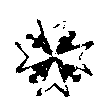
\includegraphics[width=14.726716981132075pt]{authority_rosette_native_supported_mask.png}}}}
\providecommand{\noethpIIsrcfnmark}[1]{\begingroup\renewcommand{\thefootnote}{#1}\footnotemark\addtocounter{footnote}{-1}\endgroup}
\providecommand{\noethpIIsrcfntext}[2]{\begingroup\renewcommand{\thefootnote}{#1}\footnotetext{#2}\endgroup}
\providecommand{\foreign}[1]{#1}
\begin{document}


\clearpage
\begingroup
\setcounter{footnote}{0}
% BEGIN PRODUCER UNIT 001
% Source: ../../../../noether/02_slavic_working_corpus/translations/paper01/interslavic/v001/Noether_Paper01_Interslavic_v001.tex
% Identity: 7284 B / SHA-256 94B7533CFA0F30F0197FA9622C7289A4AA563999FFDDA9D10C479866D7F4F478
\setlength{\parindent}{1.25em}
\setlength{\parskip}{0pt}
\emergencystretch=4em
% BEGIN UNIT BODY
\begin{center}
{\Large\bfseries 1. Konstrukcija sistema form za ternarnu\\ formu četvrtogo stepena}\par
\vspace{1.5em}
Sitzungsberichte Fizikalno-medicinskogo družstva v Erlangenu 39 (1907), s. 176--179
\end{center}

\vspace{4em}
\begin{center}
(Izvod iz disertacije avtorky.)
\end{center}

Sistem form ternarnoj bikvadratičnoj formy, to jest ternarnoj formy četvrtogo stepena, izsledovali Gordan, Maisano i Pascal.\footnote{P. Gordan, \emph{\foreign{Über das volle Formensystem der ternären biquadratischen Form}} $f=x_1^3x_2+x_2^3x_3+x_3^3x_1$ (Math. Annalen, tom XVII, s. 217--233, 1880); G. Maisano, 1. \emph{\foreign{Sistemi completi dei primi cinque gradi della forma ternaria biquadratica e degl' invarianti, covarianti e contravarianti di sesto grado}} (Giorn. di Battaglini XIX). 2. \emph{\foreign{Sui covarianti indipendenti di $6^\circ$ grado nei coefficienti della forma biquadratica ternaria}} (Rend. Circ. Mat. di Palermo I, 1887); E. Pascal, \emph{\foreign{Contributo alla teoria della forma ternaria biquadratica e delle sue varie decomposizioni in fattori}} (Memoria premiata dalla R. Accademia delle scienze fisiche e matematiche di Napoli, 1905).}
Gordan konstruuje polny sistem form, sostavljen iz 54 konstrukcij, za specialnu avtomorfnu formu
\[
f=x_1^3x_2+x_2^3x_3+x_3^3x_1,
\]
na osnově podobnyh principov, ktore on dal za sistemy form v binarnoj oblasti.

U Maisana za obću bikvadratičnu formu konstruovane sut formy do petogo ręda vključiteljno,\footnote{Pod "rędom" tuto razuměje se stepenj v koeficientah, a pod "stepenem" stepenj v prěměnnyh.}
a takože něktore invarianty, kovarianty i kontravarianty vyšego ręda. On slěduje metodě, ktoru Gordan priměnil v prvom tomu \emph{Mathematische Annalen} za ternarnu kubičnu formu. Pascal, koristajuči rezultatami Maisana, glavno se zanima pytanjem, kogda bikvadratična forma razkladaje se na faktory.\footnote{V svojoj drugoj kratkoj notě Maisano probuje dokazati linearnu zavisimost trěh kovariantov ręda 6 i stepena 6. Nasuprot tomu ne vpolně zakončenomu dokazu Pascal mni, že je dokazal linearnu nezavisimost tych trěh kovariantov ręda 6, a takože trěh invariantov ręda 9. No v toku mojih računenij pokazalo se, že linearno odnošenje v istině obstaje i medžu trěmi kovariantami, i medžu trěmi invariantami. V označenju Pascala jednoznačne formuly sut:
\[
0=20\Omega_1+6\Omega_2-3\Omega_3+4fC_1-12fC_2-4A\cdot\Delta,
\]
\[
0=4A^3-15AB+30C-90D+9E.
\]}

\textbf{Cilj mojih izslědovanij jest konstrukcija sistema form za obću ternarnu formu četvrtogo stepena. Najprvo dajut se samo glavne osnovy i konstruuje se tak nazyvany "odnosno polny sistem".\footnote{Za termin srav. Gordan--Kerschensteiner, \emph{\foreign{Vorlesungen über Invariantentheorie}}, tom II, s. 227.}}

Osnovna myslj pri konstrukciji sistemov ternarnyh form jest taka sama kako v binarnoj oblasti. Počinajuči od prvogo odnosno polnogo sistema, to jest od sistema form, prěnesenyh iz binarnogo slučaja, po oprěděljenom zakonu prěhodi se k sistemam s vse vyšim modulom. To ide dotud, dokud sistem někojego modula, ako sam modul vzęti za osnovnu formu, ne stane konečnym i poznanym, ili dokud modul ne možno snižiti k formam, ktore imajut invariant kako faktor. V prvom slučaju absolutno polny sistem nastaje transvekcijeju odnosno polnogo sistema so sistemom modula; v drugom slučaju odnosno polny i absolutno polny sistem sut identični. Iz obćego Hilbertovogo dokaza konečnosti sistemov form slěduje, že ta procedura mora dojti do konca.

V našem slučaju modul $(abc)$ prvogo odnosno polnogo sistema možno svesti k modulam
\[
\Delta=(abc)^2a_x^2b_x^2c_x^2\quad\text{i}\quad \nu=(abu)^4;
\]
iz toga lahko dobyvaje se odnosno polny sistem modulo $\nu$. Kako ręd modulov vybira se nyně formy
\[
\nu;\qquad \nu^{(\nu)}=(\nu\nu_1x)^4=s_x^4,
\]
\[
\nu^{(s)}=(ss'u)^4\ldots
\]
i kako daljše moduly pridajut se dvě kvadratične formy, ktore nastavajut pri konstrukciji odnosno polnogo sistema modulo $s$, imenno $u_\sigma^2$ i $t_x^2$. Potom možno pokazati, že modul slědujući po $s$, imenno $(ss'u)^4$, jest reducibilny k modulu $(\varrho,t)$. No simultanny sistem dvuh kvadratičnyh form jest konečny i poznany; tym dosegnuty jest vyše označeny konec. Odnosno polny sistem modulo $(\varrho,t)$ daje 331 konstrukcij. ---

Dodam ješče několiko ukazanij o priměnjenoj metodě.

Osnovny proces tvorjenja form, proces kontrakcije, v ternarnoj oblasti možno oprěděliti tak.

Ako v simboličnom produktu
\[
s_x^m t_x^n u_\sigma^\mu u_\tau^\nu
\]
zaměniti pary faktorov
\[
\begin{array}{c|c|c|c|c}
 & s_xt_x & u_\sigma u_\tau & s_xu_\sigma\ \text{ili}\ s_xu_\tau & t_xu_\tau\ \text{ili}\ t_xu_\sigma\\
\text{odnošno s} & (stu) & (\sigma\tau x) & s_\sigma\ \text{ili}\ s_\tau & t_\tau\ \text{ili}\ t_\sigma\\
\text{kontrakcija} & \mathrm{I} & \mathrm{II} & \mathrm{III} & \mathrm{IV}
\end{array}
\]
togda nastavajuče formy sut dobjene iz počętkovoj formy kontrakcijam.\footnote{Gordan, Math. Annalen, tom XVII, s. 219.}

Pri tom možno vse ješče položiti $s_\sigma=0$ i $t_\tau=0$. Za vzajemnu svęz medžu pojedinymi kontrakcijami imaje město slědujuća teorema.

\textbf{Kontrakcije I i II sut osnovne kontrakcije. Iz njih, nezavisno od poręda skladanja, možno sostaviti kontrakcije III i IV. Drugymi slovami: da by se stvorili vse formy, ktore nastavajut iz danogo izraza kontrakcijam, dostatočno jest priměnjati samo kontrakcije I i II.}\footnote{Teorema ima izključenje v slučaju, kogda $n$ i $\mu$, odnošno $m$ i $\nu$, jednočasno isčezajut; togda ręd form snižaje se k diagonalnomu členu.}

Pod "rędom form" razumějemo početnu formu zajedno so vsimi formami, ktore iz njej nastavajut povtornym kontrakcijam samej so soboju. Po teoremi ręd form
\[
s_x^m t_x^n u_\sigma^\mu u_\tau^\nu
\]
možno razměstiti v pręmougolnoj shemě. Pri idenju v toj shemě dobyvaje se:
\begin{enumerate}
\item jednu kolonu na pravo -- vse formy, ktore nastavajut iz susědnyh form kontrakcijam I;
\item jeden ręd v niz -- vse formy, ktore nastavajut iz form nad nimi kontrakcijam II.
\end{enumerate}
Tak dobyvajut se vse formy, ktore nastavajut kontrakcijam.

Pod tymi prědpoloženjami teoremy o reducentah možno izrekti v najobćejšej formě, pod oprěděljenjem
\begin{center}
\textbf{reducent jest reducibilny ręd form.}
\end{center}
Obća redukcijska teorema potom glasi:

\begin{center}
\textbf{Ako početna forma ręda form jest reducibilna zato, že jeden iz jej členov nastal kontrakcijam s reducentom, i ako konečna forma toga ręda nastala jest iz togo samogo člena kontrakcijam, togda cěly ręd form jest reducibilny.}
\end{center}

Kako daljše metody redukcije trěba nazvati:
\begin{enumerate}
\item tak nazyvanu dvojnu redukciju, to jest redukciju jednoj formy dvoma sposobami, da by se dobilo odnošenje medžu vyšimi formami;
\item kontrakcija s formami, ktore razkladajut se na faktory; ta metoda čęstično ima harakter redukcije s pomočju reducentov, a čęstično harakter dvojnoj redukcije.
\end{enumerate}
% END UNIT BODY
% END PRODUCER UNIT 001
\endgroup


\clearpage
\begingroup
\setcounter{footnote}{0}
% BEGIN PRODUCER UNIT 002
% Source: ../../../../noether/02_slavic_working_corpus/translations/paper02/interslavic/v001/Noether_Paper02_Introduction_Interslavic_v001.tex
% Identity: 6814 B / SHA-256 D4EBD958552D375AACD91F5E92941B0FD98E34B1992B16EAB5FD953AD0946C7C
\setlength{\parindent}{1.25em}
\setlength{\parskip}{0pt}
\emergencystretch=4em
% BEGIN UNIT BODY
\begin{center}
{\Large\bfseries 2. Konstrukcija sistema form za ternarnu\\ bikvadratičnu formu}\par
\vspace{1.5em}
\emph{\foreign{Journal für die reine und angewandte Mathematik}} 134 (1908), s. 23--90 i dvě tabely
\end{center}

\vspace{3em}

\begin{center}
\textbf{Vvod.}
\end{center}

Sistem form ternarnoj bikvadratičnoj formy izslědovali Gordan, Maisano i Pascal.\footnote{Kratky izvod iz vvoda i glavy I pojavil se v \emph{\foreign{Sitzungsberichte der physikalisch-medizinischen Sozietät Erlangen 1907}}, s. 176--179.}\footnote{P. Gordan, \emph{\foreign{Über das volle Formensystem der ternären biquadratischen Form}}
\[
f=x_1^3x_2+x_2^3x_3+x_3^3x_1.
\]
(\emph{Math. Annalen}, tom XVII (1880), s. 217--233.)
G. Maisano, 1) \emph{\foreign{Sistemi completi dei primi cinque gradi della forma ternaria biquadratica e degl' invarianti, covarianti e contravarianti di sesto grado}}. (Giorn. di Battaglini XIX.)
2) \emph{\foreign{Sui covarianti indipendenti di $6^\circ$ grado nei coefficienti della forma biquadratica ternaria}}. (Rend. Circ. Mat. di Palermo I, 1887.)
E. Pascal, \emph{\foreign{Contributo alla teoria della forma ternaria biquadratica e delle sue varie decomposizioni in fattori}}. (Memoria premiata dalla R. Accademia delle scienze fisiche e matematiche di Napoli. 1905.)}
Gordan konstruuje polny sistem form, sostavjeny iz 54 konstrukcij, za specialnu avtomorfnu formu
\[
f=x_1^3x_2+x_2^3x_3+x_3^3x_1,
\]
na osnově podobnyh principov, ktore on dal za sistemy form v binarnoj oblasti.

U Maisana za obću bikvadratičnu formu konstruovane sut vse formy do petogo ręda uključiteljno,\footnote{Pod "rędom" tuto razuměje se stepenj v koeficientah, a pod "stepenem" stepenj v prěměnnyh.}
a takože něktore invarianty, kovarianty i kontravarianty vyšego ręda. On koristaje metodu, ktoru Gordan priměnil v prvom tomu \emph{Mathematische Annalen} k ternarnoj kubičnoj formě. Pascal, opirajųći se na rezultaty Maisana, glavno se zanima pytanjem razklada bikvadratičnoj formy na faktory.\footnote{V svojoj drugoj kratkoj notě Maisano probuje dokazati linearnu zavisimost trěh kovariantov ręda 6 i stepena 6. Nasuprot tomu ne vpolně dokončenomu dokazu Pascal mni, že dokazal linearnu nezavisimost tych trěh kovariantov ręda 6, a takože trěh invariantov ręda 9. No to, že linearno odnošenje v istině obstaje medžu trěmi kovariantami, s jednoj strany, i trěmi invariantami, s drugoj strany, pokazujut formuly (13), § 11, i (22), primětka k § 17, tutoj raboty, kde ta odnošenja sut dana jednoznačno. Po informaciji Pascala protivorěčje objasnjaje se čislovoj pogrěškoju v izrazu jego kontravarianta $p$ (tuto označenogo $\varrho$), s. 46 jego statji.}

{\itshape Cilj slědujućih izslědovanij jest konstrukcija sistema form za obću ternarnu bikvadratičnu formu. V toj rabotě dajut se samo glavne osnovy i konstruuje se tak nazyvany "odnosno polny sistem".\footnote{Za termin gledati § 3a.}}

Rabota těsno primykaje k rabotě Gordana; no principy, ktore tam byli dane samo v obćem vidu, trěba bylo najprvo izrabotati v podrobnostjah. S pomočju teoremy o svęzi medžu kontrakcijami i prěz vvedenje "ręda form" (§ 1) redukcijske teoremy formulujut se točno i doplnjajut se (§ 3), dokolě rekursivna konstrukcija specialnyh razvitij v rędy (§ 2) daje računno sredstvo za stvarno provedenje redukcij.

Osnovna myslj konstrukcije sistemov ternarnyh form jest taka sama kako v binarnoj oblasti. Počinajući od prvogo odnosno polnogo sistema --- sistema form prěnesenyh iz binarnogo slučaja, --- po oprěděljenom zakonu prěhodi se k sistemam s vse vyšim modulom. Ta postupnost ide dotud, dokud sistem někojego modula, ako sam modul vzęti za osnovnu formu, ne stane konečnym i poznanym, ili dokud modul ne možno svesti k formam, ktore imajut invarianty kako faktory. V prvom slučaju absolutno polny sistem nastaje transvekcijeju odnosno polnogo sistema so sistemom modula; v drugom slučaju odnosno polny i absolutno polny sistem sut identične. Iz obćego Hilbertovogo dokaza konečnosti sistemov form slěduje, že ta procedura mora dojti do konca.

V našem slučaju modul $(abc)$ prvogo odnosno polnogo sistema (§ 4) svodi se k modulam
\[
\Delta=(abc)^2a_x^2b_x^2c_x^2\quad\text{i}\quad \nu=(abu)^4
\]
(§ 5), a potom nahodi se odnosno polny sistem modulo $\nu$ (§ 6). Ty rezultaty sut už dane v rabotě Gordana za obću bikvadratičnu formu; naš sposob izvoda jednak lehče prěnosi se na formy vyšego stepena.

Kako ręd modulov nyně vybirajemo formy (§ 7):
\[
\nu,\qquad \nu(\nu)=(\nu\nu_1x)^4=s_x^4,\qquad \nu(s)=(ss'u)^4,\ldots .
\]

Pri konstrukciji odnosno polnogo sistema modulo $s$ dvě kvadratične formy, nastavajuće v sistemu, $u_\varrho^2$ i $t_x^2$, pridajut se kako moduly (§§ 9 i 10), i odtud konstruuje se odnosno polny sistem modulo $(s,\varrho,t)$. Potom pokazuje se (§ 17), že modul $(ss'u)^4$ jest reducibilny k modulam $\varrho$ i $t$. Prěz to slědujući vyši sistem prěhodi v odnosno polny sistem modulo $(\varrho,t)$. No simultanny sistem dvuh kvadratičnyh form jest konečny i poznany, a v obćem slučaju sostavjen jest iz 20 konstrukcij;\footnote{Srav. Clebsch--Lindemann, \emph{\foreign{Vorlesungen über Geometrie}} (tom I, s. 288 i dalje), sistem dvuh kogredientnyh form. Gordan, \emph{\foreign{Über Büschel von Kegelschnitten}} (\emph{Math. Ann.}, tom XIX, s. 530), sistem dvuh kontragredientnyh form.}
tym s konstrukcijeju odnosno polnogo sistema modulo $(\varrho,t)$ dosegnuty jest vyše označeny konec. Transvekcija togo sistema so sistemom $(\varrho,t)$ za konstrukciju absolutno polnogo sistema ostaje zadržana za pozdnějši čas.

Kako odnosno polny sistem modulo $(\varrho,t)$ najdene sut 331 konstrukcije; v prilagajenej tabeli one sut uporędkovane po stepenu v prěměnnyh $x$ i $u$.

Na koncu dajemo pregled vvedenyh simbolov:
\begin{align*}
f&=a_x^4,\\
\theta&=\theta_x^4u_\vartheta^2=(abu)^2a_x^2b_x^2,\\
K&=K_x^6u_k^3=(a\theta u)u_\vartheta^2a_x^3\theta_x^3,\\
j&=u_j^6=(a\theta u)^4u_\vartheta^2,\\
\Delta&=\Delta_x^6=a_\vartheta^2a_x^2\theta_x^4=(abc)^2a_x^2b_x^2c_x^2,\\
N&=N_x^8u_\eta=(a\Delta u)a_x^3\Delta_x^5,\\
\nu&=u_\nu^4=(abu)^4,\\
H&=H_x^2u_\eta^4=(\nu\nu_1x)^2u_\nu^2u_{\nu_1}^2,\\
L&=L_x^3u_l^6=(\nu\eta x)H_x^2u_\nu^3u_\eta^3,\\
g&=g_x^6=(\nu\eta x)^4H_x^2,\\
\sigma&=u_\sigma^6=H_\nu^2u_\nu^2u_\eta^4,\\
s&=s_x^4=(\nu\nu_1x)^4,\\
Z&=Z_x^4u_\zeta^2=(ss'u)^2s_x^2s_x'^2,\\
\varrho&=u_\varrho^2=\theta_\nu^4u_\vartheta^2,\\
t&=t_x^2=a_\eta^4H_x^2,\\
i&=a_\nu^4,\\
J&=s_\nu^4.
\end{align*}
% END UNIT BODY
% END PRODUCER UNIT 002
\endgroup


\clearpage
\begingroup
\setcounter{footnote}{0}
% BEGIN PRODUCER UNIT 003
% Source: ../producer_units/Noether_Paper02_Section01_Interslavic_v001.tex
% Identity: 7674 B / SHA-256 594F093A49D5FF186EA9126E0757B635F45EA2ED8391FAC1AD117D3308033998
\setlength{\parindent}{1.25em}
\setlength{\parskip}{0pt}
\emergencystretch=4em
% BEGIN UNIT BODY
\begin{center}
{\Large\bfseries Glava I. \quad Obće teoremy o ternarnyh formah.}
\end{center}

\begin{center}
\textbf{§ 1. \quad Proces kontrakcije. \quad Rędy form.}
\end{center}

Osnovny proces tvorjenja form jest proces kontrakcije, ktory v ternarnoj oblasti možno oprěděliti slědujućim sposobom. Nehaj bude dany simboličny produkt
\[
s_x^m t_x^n u_\sigma^\mu u_\tau^\nu .
\]
Ako pary faktorov
\[
s_xt_x\qquad u_\sigma u_\tau\qquad s_xu_\sigma\ \text{ili}\ s_xu_\tau
\qquad t_xu_\tau\ \text{ili}\ t_xu_\sigma
\]
zaměniti odnošno s
\[
(stu)\qquad (\sigma\tau x)\qquad s_\sigma\ \text{ili}\ s_\tau
\qquad t_\tau\ \text{ili}\ t_\sigma,
\]
to jest so kontrakcijami
\[
\text{I}\qquad\text{II}\qquad\text{III}\qquad\text{IV},
\]
togda nastavajuće formy nastavajut iz počętkovoj formy prěz kontrakciju.\footnote{Gordan, \emph{Math. Annalen}, tom XVII, s. 219.}

Pri tom izraz $s_x^m t_x^n u_\sigma^\mu u_\tau^\nu$ možno razuměti ili kako stvarny produkt dvuh form $S\cdot T$, ili kako jedinu formu s několiko rędami simbolov:
\[
s_x^m t_x^n u_\sigma^\mu u_\tau^\nu=A_x^{m+n}u_x^{\mu+\nu}.
\]
V prvom slučaju govorimo o kontrakciji formy $S$ s formoju $T$, v drugom slučaju o «kontrakciji formy $A$ samej so soboju». Dlja kratkosti v slědujućem vsegda prědpokladamo (to v istině jest slučaj pri vsih pozdněje razgledanyh formah), že
\[
\tag{a}
s_\sigma^\lambda=0,\qquad t_\tau^\chi=0
\]
za vsake $\lambda$ i $\chi$, različne od nule, i zajedno s kakymikoli drugymi kontrakcijami. To govori, že forma $s_x^m t_y^n u_\sigma^\mu u_\tau^\nu$ jest tak nazyvana «normalna forma», to jest pri priměnjenju $\Omega$-procesa ona isčezaje i po prěměnnyh $x$ i $u$, i po prěměnnyh $y$ i $v$.

Uslovje (a) zato ne jest ograničenje; jego možno vsegda dosegnuti.\footnote{Srav. Gordan, \emph{Math. Annalen}, tom V, s. 104.}

Za svęz medžu pojedinymi kontrakcijami imaje město slědujuća teorema:

{\itshape Teorema I. Kontrakcije I i II sut osnovne kontrakcije; iz njih, nezavisno od poręda skladanja, možno sostaviti kontrakcije III i IV. Drugymi slovami: da by se stvorili vse formy nastavajuće iz danogo izraza prěz kontrakciju, trěba priměnjati samo kontrakcije I i II.}

Dokaz. Po teoremě identičnosti, odnošno po teoremě produkta za matrice, s uvagoj na (a) dobyvajemo
\[
(\widehat{st}\sigma x)=-t_\sigma,\qquad
(\widehat{\sigma\tau}su)=-s_\tau,
\]
\[
(\widehat{st}\tau x)=s_\tau,\qquad
(\widehat{\sigma\tau}tu)=t_\sigma,
\]
\[
(stu)(\sigma\tau x)=s_\tau+t_\sigma-u_x\,s_\tau t_\sigma .
\]
Zato prěz skladanje kontrakcij I i II nastavajut kontrakcije III i IV; to jest takože pri priměnjenju kontrakcije II k kontrakciji I, to jest k faktoram $(stu)u_\sigma u_\tau$, kako i pri priměnjenju kontrakcije I k kontrakciji II, to jest k faktoram $(\sigma\tau x)s_xt_x$.

Pod {\itshape rędom form}\footnote{Srav. Clebsch, \emph{\foreign{Über eine Fundamentalaufgabe der Invariantentheorie}} (\foreign{Abh. der Gött. Ges. d. Wiss.}, tom XVII): § 17 i konec § 18. «Ręd form» razlikuje se od tamo vvedenogo «vlastno reduciranogo ekvivalentnogo sistema» principom uporędkovanja po vyšših formah.}
razumějemo početnu formu zajedno so vsimi formami, ktore iz njej nastali sut kontrakcijam samej so soboju, i označujemo ręd form početnoju formoju. «Vyša forma» tuto znači vsaku formu s bolje mnogym kontrakcijam samej so soboju; medžu ravnopravnymi kontrakcijami $s_\tau$ i $t_\sigma$ jedno mora byti normovano kako vyše. Po zakonu tvorjenja ręda form slěduje:

1) Vsaka forma ręda form jest linearna v simbolah početnoj formy.

2) Ręd form jest jednoznačno oprěděljen za početne formy s po dvěma rędami kontragredientnyh simbolov; pri početnyh formah s bolje rędami simbolov jego trěba jednoznačno normovati vyznačenjem specialnyh kontrakcij medžu tymi, ktore sut svęzane teoremoju identičnosti.

Po teoremě I ręd form $s_x^m t_x^n u_\sigma^\mu u_\tau^\nu$ ($m>n;\ \mu>\nu$) možno razměstiti po slědujućej pręmougolnoj shemě:
\begingroup\small
\[
\begin{array}{c|c|c|c|c}
s_x^m t_x^n u_\sigma^\mu u_\tau^\nu
& (stu)
& (stu)^2
& \cdots
& \noethpIIrosette\\[0.3em]
(\sigma\tau x)
& t_\sigma,\ s_\tau
& t_\sigma(stu),\ s_\tau(stu)
& \cdots
& \vdots\\[0.3em]
(\sigma\tau x)^2
& t_\sigma(\sigma\tau x),\ s_\tau(\sigma\tau x)
& t_\sigma^2,\ t_\sigma s_\tau,\ s_\tau^2
& \cdots
& \vdots\\[0.3em]
\vdots&\vdots&\vdots&\ddots&\vdots\\[0.3em]
(\sigma\tau x)^\nu
& t_\sigma(\sigma\tau x)^{\nu-1},\ s_\tau(\sigma\tau x)^{\nu-1}
& t_\sigma^2(\sigma\tau x)^{\nu-2},\ t_\sigma s_\tau(\sigma\tau x)^{\nu-2},\ s_\tau^2(\sigma\tau x)^{\nu-2}
& \cdots
& \vdots\\[0.3em]
\vdots
& t_\sigma(\sigma\tau x)^\nu
& t_\sigma^2(\sigma\tau x)^{\nu-1},\ t_\sigma s_\tau(\sigma\tau x)^{\nu-1}
& \cdots
& \vdots\\[0.3em]
\vdots
& \vdots
& t_\sigma^2(\sigma\tau x)^\nu
& \cdots
& \vdots
\end{array}
\]
\endgroup
i odnošno prodolženu nižnju čęst
\begingroup\small
\[
\begin{array}{r@{\quad}c}
\noethpIIrosette\noethpIIsrcfnmark{*)}
&
\begin{array}{c|c|c}
(stu)^n & \cdots & \cdots\\[0.3em]
t_\sigma(stu)^{n-1},\ s_\tau(stu)^{n-1}
& s_\tau(stu)^n & \cdots\\[0.3em]
t_\sigma^2(stu)^{n-2},\ t_\sigma s_\tau(stu)^{n-2},\ s_\tau^2(stu)^{n-2}
& t_\sigma s_\tau(stu)^{n-1},\ s_\tau^2(stu)^{n-1}
& s_\tau^2(stu)^n .
\end{array}
\end{array}
\]
\endgroup
\noethpIIsrcfntext{*)}{Tuto, i podobno v slědujućem, nižnju čęst označenu zvězdočkoju trěba priložiti k takože označenomu městu v pravoj gornoj čęsti shemy.}

Tuto dobyvajemo, ako se ide

1) jednu kolonu na pravo, vse formy, ktore nastavajut iz susědnyh form prěz kontrakciju I;

2) jeden ręd v niz, vse formy, ktore nastavajut iz form stojećih nad nimi prěz kontrakciju II;

i s tym vse formy, ktore nastavajut prěz kontrakciju.

Libovoljna forma cělogo ręda form, $t_\sigma^\kappa s_\tau^\lambda(stu)^\mu$ ili $t_\sigma^\kappa s_\tau^\lambda(\sigma\tau x)^\nu$, tvori početok novogo ręda form. On sostoji se iz vsih tych form pręmougolnoj shemy, ktore imajut formu $t_\sigma^\kappa s_\tau^\lambda(stu)^\mu$ ili $t_\sigma^\kappa s_\tau^\lambda(\sigma\tau x)^\nu$ kako lěvy gorny kut i imajut faktor $t_\sigma^\kappa s_\tau^\lambda$.

Dodatna primětka. Teorema I ima izključenje v slučaju, kogda čisla $n$ i $\mu$ (odnošno $m$ i $\nu$) stanut ravne nuli, tako že kontrakcije I, II i IV už ne obstajajut, no kontrakcija III (odnošno IV) ješče obstaje. V tom slučaju rędom form nazyvajemo diagonalny člen shemy:
\[
\begin{array}{ccccc}
s_x^m u_\tau^\nu &&&& t_x^n u_\sigma^\mu\\
& s_\tau && t_\sigma &\\
& s_\tau^2 && t_\sigma^2 &\\
&&\ddots&&\\
&&s_\tau^\nu && t_\sigma^\mu .
\end{array}
\]
V soglasnosti s odsutnostju kontrakcij I i II, razvitje v ręd po polarah ręda form v tom slučaju vsegda snižaje se k početnomu členu; ale teoremy o reducentah ostavajut v silě.
% END UNIT BODY
% END PRODUCER UNIT 003
\endgroup


\clearpage
\begingroup
\setcounter{footnote}{0}
% BEGIN PRODUCER UNIT 004
% Source: ../../../../noether/02_slavic_working_corpus/translations/paper02/interslavic/v001/Noether_Paper02_Section02_Interslavic_v001.tex
% Identity: 6938 B / SHA-256 AF6E7C4F4E44E8016C1E63C958CD3F543AF7BAC3A3F37450A1AA15635636B801
\setlength{\parindent}{1.25em}
\setlength{\parskip}{0pt}
\emergencystretch=4em
% BEGIN UNIT BODY
\begin{center}
\textbf{§ 2. \quad Razvitja v ręd po polarah ręda form.}
\end{center}

Za formy s $n$ prěměnnymi eksplicitno sut postavjene dvě vrsty razvitij v ręd\footnote{Srav. Gordan, \emph{\foreign{Über Kombinanten}}, § 2 i 5 (\emph{Math. Ann.}, tom V).}:

1) za formy s po jednym rędom kontragredientnyh prěměnnyh, $s_x^m u_\tau^\nu$, ręd, ktory ide po stepenjah $u_x$ i ktorego koeficienty sut «normalne formy»;

2) za formy s dvěma rędami kogredientnyh prěměnnyh $s_x^m t_x^n$ razvitje po polarah elementarnyh kovariantov (polarah ręda form $s_x^m t_x^n$), ktore v ternarnom slučaju glasi tak\footnote{Srav. Study, \emph{\foreign{Methoden zur Theorie der ternären Formen}} (Teubner 1889) II. § 7. V razlikě od tamošnjego vyvoda naš daje metod brzogo računogo oprěděljenja čislovyh koeficientov $C_{pr\varrho}$. Razvitje Clebscha--Studyja pri specializaciji a), a') imalo by oblik:
\[
(stu)^\mu u_\tau^{\nu-\kappa}v_\tau^\kappa s_x^m t_x^{\,n-\lambda}(tuv)^\lambda
=\sum_{p,r,\varrho} C_{pr\varrho}
\bigl[s_\tau^\varrho(stu)^{\mu+r-\varrho}\bigr]_{\widehat{uv}^{\lambda-r+\varrho}v^{\nu-\varrho},\,u^p,\,(vw=\widehat{xw})},
\]
i zato ne dopušča uproščenja, ktore v našem razvitju nastaje už v toku računa, kogda se znajet, že vse členy s faktorom $u_x$ trěba izpustiti.}:
\[
\tag{I}
s_x^m t_x^{n-\lambda}t_y^\lambda
=\sum_{\varrho}
\frac{\binom{m}{\varrho}\binom{\lambda}{\varrho}}
{\binom{m+n-\varrho+1}{\varrho}}
\bigl[(st\widehat{xy})^\varrho s_x^{m-\varrho}t_x^{n-\varrho}\bigr]_{y^{\lambda-\varrho}}.
\]

My kombinujemo oba razvitja tako, že za formy s po dvěma rędami kontragredientnyh prěměnnyh
\[
s_x^m t_x^{n-\lambda}t_y^\lambda u_\sigma^\mu u_\tau^{\nu-\kappa}v_\tau^\kappa
\]
postavljamo razvitja po stepenjah $u_x$, ktoryh koeficienty sut složene polary ręda form $s_x^m t_x^n u_\sigma^\mu u_\tau^\nu$, vzęte po prěměnnyh $x$ i $u$.

Dostatočno jest postaviti ręd za dvě kontragredientne rędy simbolov (odnošno prěměnnyh), zato že prěz sjedinjanje vsakyh dvuh rędov simbolov (prěměnnyh) v jeden novy ręd možno formy s bolje rędami simbolov (prěměnnyh) svesti k tomu slučaju.

Da by se dosegnulo, že vse formy ręda form imajut samo po dva rędy simbolov ili prěměnnyh, specializujemo:
\[
\begin{array}{ll}
\text{a) } \sigma=\widehat{st}, & \text{a') } y=\widehat{uv},\\[0.3em]
\text{b) } s=\widehat{\sigma\tau}, & \text{b') } v=\widehat{xy},
\end{array}
\]
i provodimo razvitje za specializaciju a), a').

Prěmym prěnosom razvitja I dobyvajut se složene polary za formy $(stu)^\mu s_x^m t_x^{n-\lambda}t_y^\lambda$, medžutym za formy $(stu)^\mu u_\tau^{\nu-\kappa}v_\tau^\kappa s_x^m t_x^{n-\lambda}t_y^\lambda$ vměsto složenyh polarov nastavajut členy takogo roda, ktoryh ocěnjenje potrěbuje vvedenje vse novyh pomocnyh prěměnnyh, ktore trěba identifikovati jedinorazno na koncu; prěz to račun staje nepotrěbno skomplikovany.

Zato izbirajemo neprěmy put: prědstavjamo složene polary vsih form ręda form, to jest izrazy
\[
\bigl[s_\tau^\varrho(stu)^{\mu-\varrho+r}\bigr]_{y^\lambda}^{v^\kappa}
\]
prěz početne členy tych polarov i, obratom nastavajućego rekursivnogo sistema ravnanij, dobyvajemo želano razvitje po polarah.

Po principu prěnosa za $\lambda$-tu polaru formy $s_x^m t_x^n:[s_x^m t_x^n]_{y^\lambda}$ ($\lambda\le n$) imaje město slědujuće razvitje (slučaj $\lambda>n$ svodi se k prvomu prěz razvitje $[s_y^m t_y^n]_{x^{m+n-\lambda}}$)\footnote{Gordan, \emph{\foreign{Die Resultante binärer Formen}} (Kap. I, § 5). Rend. Circ. Mat. di Palermo XXII. 1906.}:
\[
\bigl[s_x^m t_x^n\bigr]_{y^\lambda}
=\sum_r (-1)^r\,
\frac{\binom{m}{r}\binom{\lambda}{r}}{\binom{m+n}{r}}\,
(st\widehat{xy})^r s_x^{m-r}t_x^{n-\lambda}t_y^{\lambda-r},
\]
i odnošno za $\kappa$-tu polaru formy $u_\sigma^\mu u_\tau^\nu:[u_\sigma^\mu u_\tau^\nu]_{v^\kappa}$
\[
\bigl[u_\sigma^\mu u_\tau^\nu\bigr]_{v^\kappa}
=\sum_\varrho (-1)^\varrho\,
\frac{\binom{\mu}{\varrho}\binom{\kappa}{\varrho}}{\binom{\mu+\nu}{\varrho}}\,
(\sigma\tau\widehat{uv})^\varrho u_\sigma^{\mu-\varrho}u_\tau^{\nu-\kappa}v_\tau^{\kappa-\varrho}.
\]

Množenjem, s vvedenjem specializacije a) i a'), slěduje
\[
\begin{aligned}
\bigl[s_x^m t_x^n(stu)^\mu u_\tau^\nu\bigr]_{\widehat{uv}^{\lambda}}^{v^\kappa}
={}&
\sum_{r,\varrho}c_{r\varrho}\,
(st\widehat{uv})^r(st\widehat{uv})^\varrho
s_x^{m-r}t_x^{n-\lambda}(tuv)^{\lambda-r}(stu)^{\mu-\varrho}
u_\tau^{\nu-\kappa}v_\tau^{\kappa-\varrho},
\end{aligned}
\]
i iz togo, prěz razvitje po stepenjah $u_x$ s vyznačenjem prvogo člena ($\sum'_{r,\varrho}$ znači, že člen $r=0$, $\varrho=0$ trěba izpustiti) i s uvagoj na (a) na s. 26,
\[
\tag{II}
\begin{aligned}
&s_x^m t_x^{n-\lambda}(tuv)^\lambda(stu)^\mu u_\tau^{\nu-\kappa}v_\tau^\kappa\\
&\quad =
\bigl[s_x^m t_x^n(stu)^\mu u_\tau^\nu\bigr]_{\widehat{uv}^{\lambda}}^{v^\kappa}\\
&\qquad
-\sum_{r,\varrho}' c_{r\varrho}\,s_\tau^\varrho(stu)^{\mu-\varrho+r}
u_\tau^{\nu-\kappa}v_\tau^{\kappa-\varrho}
s_x^{m-r}t_x^{n-\lambda}(tuv)^{\lambda-r+\varrho}v_x^r\\
&\qquad
+u_x\sum_{\varrho}\sum_{r=1}^{\lambda} c_{r\varrho}\,
s_\tau^\varrho(stu)^{\mu-\varrho+r-1}(stv)
u_\tau^{\nu-\kappa}v_\tau^{\kappa-\varrho}
s_x^{m-r}t_x^{n-\lambda}(tuv)^{\lambda-r+\varrho}v_x^{r-1}\\
&\qquad
\vdots\\
&\qquad
-(-1)^\lambda u_x^\lambda\sum_\varrho c_{\lambda\varrho}\,
s_\tau^\varrho(stu)^{\mu-\varrho}(stv)^\lambda
u_\tau^{\nu-\kappa}v_\tau^{\kappa-\varrho}
s_x^{m-\lambda}t_x^{n-\lambda}(tuv)^\varrho,
\end{aligned}
\]
kde
\[
c_{r\varrho}=(-1)^{r+\varrho}\cdot
\frac{\binom{m}{r}\binom{\lambda}{r}}{\binom{m+n}{r}}\cdot
\frac{\binom{\mu}{\varrho}\binom{\kappa}{\varrho}}{\binom{\mu+\nu}{\varrho}}
\qquad
\begin{array}{l}
\text{za }\lambda\le n,\\
\kappa\le\nu.
\end{array}
\]
i odnošno za ostale kombinacije čisel
\[\lambda,n;\kappa,\nu.\]
Izraz
\[s_x^m t_x^{n-\lambda}(tuv)^\lambda(stu)^\mu u_\tau^{\nu-\kappa}v_\tau^\kappa\]
jest zato svedeny k složenej polari i, pri priměnjenju identičnosti
\[
(stv)u_\tau=(stu)v_\tau-s_\tau(tuv),
\]
k sumě analogno stvorenyh izrazov, ktore odpovědajut vyšim formam ręda form.

Prěz iteraciju prihodimo k razvitju:
\[
\tag{III}
s_x^m t_x^{n-\lambda}(tuv)^\lambda(stu)^\mu u_\tau^{\nu-\kappa}v_\tau^\kappa
=
\sum_{p,r,\varrho}u_x^p\,C_{pr\varrho}\cdot
\bigl[s_\tau^\varrho(stu)^{\mu-\varrho+r}\bigr]_{\widehat{uv}^{\lambda-r+\varrho}v^{\kappa-\varrho+p},\,v_x^{r-p}}.
\]
Čislove koeficienty $C_{pr\varrho}$ jednoznačno i rekursivno računjut se iz koeficientov $c_{r\varrho}$, $c'_{r\varrho}$ sistema ravnanij, ktory nastaje prěz iteraciju (II.) (srav. priměr na s. 42). Analogna razvitja nastavajut pri ostalyh specializacijah.
% END UNIT BODY
% END PRODUCER UNIT 004
\endgroup


\clearpage
\begingroup
\setcounter{footnote}{0}
% BEGIN PRODUCER UNIT 005
% Source: ../../../../noether/02_slavic_working_corpus/translations/paper02/interslavic/v001/Noether_Paper02_Section03_Interslavic_v001.tex
% Identity: 7634 B / SHA-256 A36275222B056854F2A2488BCDF0B823A8E7DE9A24C8836456EDD48F6A84C222
\setlength{\parindent}{1.25em}
\setlength{\parskip}{0pt}
\emergencystretch=4em
% BEGIN UNIT BODY
\begin{center}
\textbf{§ 3. \quad Redukcijne teoremy.}
\end{center}

Znane teoremy o redukciji form i sistemov form trěba nyně svęzati s paragrafami 1 i 2; za to potrěbne sut něktore oprěděljenja, vzęte iz teorije binarnyh form.

a) Kako {\itshape relativno polny sistem} po modulu danogo ręda form označajemo sistem form s takym svojstvom: vse tvorjenja, ktore nastavajut prěz kontrakciju libovoljnogo produkta tyh form, možno izraziti kako cěle racionalne funkcije form sistema, do dodatnogo člena izrazov, ktore nastali prěz kontrakciju sistemnyh form so sistemom modula\footnote{Gordan--Kerschensteiner, \emph{\foreign{Vorlesungen über Invariantentheorie}}, tom II, s. 227.}.

b) Formu nazyvajemo {\itshape reducibilnoju}, kogda ju možno izraziti prěz formy, ktore imajut invarianty kako faktory, ili prěz «vyše formy»; to jest prěz vyše formy cělogo ręda form, k ktoromu ona naleži, ili prěz formy, ktore sodrživajut simboly modula vo vyšem porędku.

Teoremy o reducentah\footnote{Gordan, \emph{Math. Annalen}, tom XVII, s. 222.} možno v najobćejšoj formě izrekti tak:

Oprěděljenje: {\itshape reducent jest reducibilny ręd form.}

{\itshape Teorema II. Jestli početna forma ręda form jest reducibilna zato, že jeden iz jej členov nastal prěz kontrakciju s reducentom (ima reducent kako faktor), i jestli konečna forma ręda form nastala iz togo samogo člena prěz kontrakciju, togda cěly ręd form jest reducibilny}\footnote{Uproščenje, ktore nastaje prěz teoremu II, možno pokazati na slědujućem priměru. Za specialnu formu $f=x_1^3x_2+x_2^3x_3+x_3^3x_1$ izraz $a_y^2a_x^2u_y^2$ jest reducent. Iz togo po teoremě II slěduje redukcija ręda form
\[
\theta_\nu(\vartheta\nu x)\theta_x^3u_\vartheta u_\nu^2
=
a_\nu^2(abu)-a_\nu b_\nu(aba),
\]
zato že $\theta_\nu^4=a_\nu^2b_\nu^2(abu)^2$ nastala iz člena $a_\nu^2(abu)$ prěz kontrakciju. U Gordana, tamže, s. 231, nasuproti tomu, redukcija form
\[
\theta_\nu(\vartheta\nu x),\quad \theta_\nu(\vartheta\nu x)^2,\quad
\theta_\nu^2,\quad \theta_\nu^2(\vartheta\nu x),\quad
\theta_\nu^2(\vartheta\nu x)^2
\]
provodit se pojedinačno.}.

Dokaz: Ręd form nastaje iz početnogo člena prěz kontrakciju samogo sebe, to jest s jednoj strany prěz vyše kontrakcije s reducentom, s drugoj strany prěz kontrakciju reducenta samogo sebe. V obojih slučajah, po § 2, možno vse formy ręda form prědstaviti kako polary (prěkrivanja) nad rędom form reducenta.

Zaključenje od početnoj formy k cělomu rędu form už ne imaje město pri ostalyh metodah redukcije. To sut:

1) tak nazyvana «dvojna redukcija».

Pod tym razumějemo redukciju izraza, ktory ima dva medžusobno nezavisne reducenty kako faktory, dvojim sposobom; prěz to nastavajut relacije medžu vyšimi formami, k ktorym bylo reducirano.

Sistematičnym priměnjenjem «dvojnoj redukcije» trěba s jednoj strany dobiti vse relacije\footnote{Tako sut, napriměr, prěz «dvojnu redukciju» najdene: redukcija formy $a_\eta^4$ (§ 10), jedinoj formy, ktoru Maisano zbytočno vnesl v sistem; potom v primětki k uvodu spomenute relacije medžu 3 kovariantami i 3 invariantami.}; s drugoj strany, jestli «dvojna redukcija», priměnjena k različnym izrazam, ne daje novyh relacij, imamo i kriterij nezavisnosti vyšših form i kontrolu računa.

2) {\itshape Kontrakcija s razložimymi formami.}

Pod «razložimymi formami» -- s malym obobćenjem običnogo pojma -- razumějemo formy, ktore možno izraziti prěz produkty form nižšego stepena i prěz «vyše» formy. Produkty form pri jednokratnoj kontrakciji prěhodet v produkty; takože produkty nelinearnyh form pri dvokratnoj kontrakciji pri specializacijah a') i b') (§ 2) po teoremě produkta:
\[
a_yb_y a_xb_x=\frac12a_y^2b_x^2+\frac12b_y^2a_x^2-\frac12(ab\widehat{yx})^2.
\]
Prve polary (prěkrivanja) i něktore druge polary razložimyh form zato sut ponovno razložime formy. Iz togo slěduje:

Člen jednokratnogo (odnošno dvokratnogo) prěkrivanja nad razložimoju formoju, ktory nastal prěz jednokratnu (odnošno dvokratnu) kontrakciju s razložimoju formoju, sam staje razložima forma:

a) kogda slědujuće vyše formy v rędu form razložimoj formy razlagajut se ili stavajut reducibilne, ili takože kogda pri jednokratnoj kontrakciji nastavajut specializacije $y=\widehat{uv}$ ili $v=\widehat{xy}$;

b) kogda ostale jednokratne kontrakcije vodet k vyšim formam (srav. § 12, B. $H_k$ i $H_k(k\eta x)$).

Takovy člen prěkrivanja može takože razložiti se:

c) kogda ostale jednokratne kontrakcije vodet k nižšim formam, ktore nezavisno od kontrakcije s razložimoju formoju razlagajut se, to možno ih izraziti prěz produkty i prěz formu, ktoru trěba reducirati. Pri tom trěba vsakokratno najprvo računom ověrjati, že čislovy koeficient odgovarjajučego člena ne isčezaje identično. To jest ničto drugo než «dvojna redukcija» nižšej formy (srav. § 23, C. $H_q(\theta H u)(\theta s u)$).

Razložime formy nastavajut prěz vse jednokratne kontrakcije s funkcionalnymi determinantami\footnote{Srav. Gordan, tamže, § 3.}, kromě togo prěz něktore vyše kontrakcije. Imamo
\[
(st\widehat{yx})s_y=\frac12\,t\,s_y^2-\frac12\,s\,t_y^2+\frac12(st\widehat{yx})^2,
\]
\[
(st\widehat{yx})^2s_y^2=\frac13\,t\,s_y^3-\frac13\,s\,t_y^3+s_y(st\widehat{yx})^2-\frac13(st\widehat{yx})^3.
\]
Analogične formuly imajut město za dualistične formy
\[
(\sigma\tau\widehat{\nu u})v_\sigma
\quad\text{i}\quad
(\sigma\tau\widehat{\nu u})v_\sigma^2.
\]

Iz teoremov togo paragrafa za postavjenje vsih nereducibilnyh form, ktore nastavajut iz kontrakcije $S$ s $T$, dobyva se slědujuće pravilo:

Iděmo, počinajući s najnižšimi kontrakcijami, po libovoljnom naprijed ustanovjenom putu (napriměr po rędah ili simetrično k diagonalnomu členu) tako daleko v tvorjenju ręda form $ST$, poky ne dojdemo do formy, ktora ima reducent kako faktor. Ręd form oprěděljeny toju formoju trěba izpustiti, kogda konečna forma izpolnja uslovje postavjeno v teoremě II. Poslě izključenja vsih reducibilnyh rędov form trěba prěz priměnjenje dvojnoj redukcije odstraniti vse ostale reducibilne, i takože vse razložime formy. Města cělogo ręda form, ktore sut dvojno prěkryte nezavisno reducibilnymi rędami form, davajut povod k redukciji vyšših form (srav. § 11, D).

\clearpage
\noindent\textbf{Teorema III.}
{\itshape Formy vzęte iz binarnoj oblasti, to jest one formy, ktore nastavajut iz sistemnyh form odgovarjajučego binarnogo formy po Clebschovom principu prěnosa prěz obrubljenje, tvoręt relativno polny sistem mod $(abc)$.}

\noindent\textbf{Dokaz:}
Binarnoj relaciji, ktora govori, že formy $Q'_1,\ldots,Q'_n$ tvoręt polny sistem jednoj binarnoj osnovnoj formy:
\[
Q'-F(Q')=0=\sum_\lambda\bigl\{(ab)c_x+(bc)a_x+(ca)b_x\bigr\}\varphi_\lambda^{*}
\]
prěz obrubljenje odgovarja ternarna relacija:
\[
Q-F(Q_i)=\sum_\lambda u_x\cdot(abc)\varphi_\lambda .
\]
To jest ale oprěděljajuće ravnanje za relativno polny sistem mod $(abc)$. Za bikvadratičnu formu sistem vzętyh form sostoji se iz slědujućih form:
\[
\begin{gathered}
f=a_x^4,\qquad
\theta=\theta_x^4u_\vartheta^2=(abu)^2a_x^2b_x^2,\qquad
K=K_x^6u_k^3=(a\theta u)u_\vartheta^2a_x^3\theta_x^3,\\
j=u_j^6=(a\theta u)^4u_\vartheta^2,\qquad
\nu=u_\nu^4=(abu)^4,
\end{gathered}
\]
medžu ktorymi prve četyri tvoręt relativno polny sistem mod $((abc),\nu)$.
% END UNIT BODY
% END PRODUCER UNIT 005
\endgroup


\clearpage
\begingroup
\setcounter{footnote}{0}
% BEGIN PRODUCER UNIT 006
% Source: ../../../../noether/02_slavic_working_corpus/translations/paper02/interslavic/v001/Noether_Paper02_Section05_Interslavic_v001.tex
% Identity: 7256 B / SHA-256 5A63CC75BBB84E097916A6E1002E88D439F3832CB750E8B9CB9DD31EBF3E8735
\setlength{\parindent}{1.25em}
\setlength{\parskip}{0pt}
\emergencystretch=4em
\let\A\relax
\newcommand{\A}{\mathfrak A}
% BEGIN UNIT BODY
\begin{center}
\textbf{§ 5. \quad Svedenje modula $(abc)$ k modulam $\A$ i $\nu$.}
\end{center}

Modul $(abc)$, dany samo jednym skobkovym faktorom, v soglasju s oprěděljenjem (§ 3, a) trěba svesti k formam sistema. Drugymi slovami: ręd form $(abc)$ trěba jednoznačno normovati (srav. § 1).

\[
a_s^2a_xu_x=\frac13 a_s^3u_x=\frac13 S\cdot u_x. \tag{2}
\]
\[
\left.
\begin{aligned}
(a\A u)^2&=a_s-\frac{S}{6}u_x^2,\\
(a\A u)^3&=0.
\end{aligned}
\right\} \tag{3}
\]
\[
\left.
\begin{aligned}
\theta(s)=(ss,x)^2&=2a_t+\frac13 S\cdot\theta-\frac13 Tu_x^2,\\
\theta(t)=(tt,x)^2&=-\frac13 S\cdot a_t+\frac23 T\cdot a_s+\frac1{18}S^2\cdot\theta-\frac1{18}u_x^2\cdot S\cdot T.
\end{aligned}
\right\} \tag{4}
\]

Ręd modulov: $(abc)$; $\A$; $s$; $t$ (sistem modula $t$ sostoji se iz jedinoj formy $t$).\footnote{Gordan--Kerschensteiner, tamže, s. 134.}

Pokaže se, že formy
\[
\A=(abc)^2a_x^2b_x^2c_x^2,\qquad \nu=(abu)^4
\]
dostatočne sut kako modul, to jest že formy
\[
\begin{gathered}
\A=(abc)^2a_x^2b_x^2c_x^2,\qquad
a_\nu=(abc)(bcu)^3a_x^3,\\
a_\nu^2=(abc)^2(bcu)^2u_x^2,\qquad
i=a_\nu^4=(abc)^4
\end{gathered}
\]
oprěděljajut ręd form $(abc)$. V rędu form $a_\nu$ ne imaje formy $a_\nu^3$ po identičnosti
\[
a_\nu^3=(abc)^3a_x(bcu)=\frac13 u_x\cdot(abc)^4=\frac13 i\cdot u_x.
\]

Za svedenje modula k vyšemu modulu trěba po oprěděljenju svesti najobćejše kontrakcije, ili takože vse specialne razgledane kontrakcije s modulom, k kontrakcijam s vyšim modulom.

Najobćejše kontrakcije nastavajut v našem slučaju iz izrazov
\[
(abc)a_x^3b_y^3c_z^3,\qquad
(abc)a_x^2b_y^2c_z^2a_zb_xc_x
\]
(vzętyh iz kubičnyh form),
\[
(abc)a_xb_yc_za_x^2b_x^2c_x^2
\]
(vzętogo iz kvadratičnyh form) i prěz polarizaciju tyh izrazov.

Za izračunanje tyh izrazov prěz polary $\A$ i ręda form $a_\nu$, odnošno prěz ih početne členy, izbirajemo, kako v § 2, neprěmy put. Razvijamo polarny členy
\[
(abc)^2a_x^2b_y^2c_z^2,\qquad
a_\nu(\nu xy)(\nu yz)(\nu zx)a_xa_ya_z
=(abc)(bc\widehat{x}u)(bc\widehat{y}z)(bc\widehat{z}x)a_xa_ya_z\quad\text{i t. d.}
\]
kako linearne kombinacije izrazov so simboličnym faktorom $(abc)$ i, obratom sistema ravnanij, dobyvajemo iskane relacije, takože relaciju medžu polarami vzętymi po različnym kombinacijam prěměnnyh. Za ocěnjenje služet teorema identičnosti i teorema produkta za determinanty.

Sistem ravnanij za $(abc)a_x^3b_y^3c_z^3$ glasi:
\begingroup\small
\[
\begin{aligned}
1)\quad
\sum_3 a_\nu(\nu yz)^3a_x^3
&=6(abc)a_x^3b_y^3c_z^3
-6\sum_3(abc)a_x^3b_y^2b_zc_z^2c_y^{*},\\[0.4em]
2)\quad
3(abc)^2a_x^2b_y^2c_z^2\cdot(xyz)
-\frac12\sum_3 a_\nu^2(\nu yz)^2\nu_x^2(xyz)
&=2\sum_3(abc)a_x^3b_y^2b_zc_z^2c_y\\
&\quad-4\sum_3(abc)a_xa_ya_zb_y^2b_zc_z^2c_x,\\[0.4em]
3)\quad
a_\nu(\nu xy)(\nu yz)(\nu zx)a_xa_ya_z
&=2\sum_3(abc)a_xa_ya_zb_y^2b_zc_z^2c_x,\\[0.4em]
4)\quad
\sum_3 a_\nu(\nu yz)^3u_x^3
-\frac32\sum_3 a_\nu^2(\nu yz)^2\nu_x^2(xyz)
+\frac16 i\cdot(xyz)^3
&=6\sum_3(abc)a_xa_ya_zb_y^2b_zc_z^2c_x.
\end{aligned}
\]
\endgroup

Iz togo slěduje za
\[
(abc)a_x^3b_y^3c_z^3,
\]
i prěz analogny račun za
\[
(abc)a_x^2b_y^2c_z^2a_zb_xc_x,\qquad
(abc)a_xb_yc_za_z^2b_x^2c_x^2:
\]
\begingroup\small
\[
\begin{aligned}
(abc)a_x^3b_y^3c_z^3
&=\frac32(abc)^2a_x^2b_y^2c_z^2(xyz)
+\frac32 a_\nu(\nu xy)(\nu yz)(\nu zx)a_xa_ya_z\\
&\quad-\frac1{12}i\cdot(xyz)^3,\\[0.4em]
(\text{IV.})\quad
(abc)a_x^2b_y^2c_z^2a_zb_xc_x
&=\frac23(abc)^2a_x^2b_y^2c_z^2c_x\cdot(xyz)\\
&\quad+\frac13a_\nu(\nu xy)(\nu yz)(\nu zx)a_x^3
-\frac16 a_\nu^2(\nu xy)(\nu zx)a_x^2\cdot(xyz),\\[0.4em]
(abc)a_xb_yc_za_z^2b_x^2c_x^2
&=\frac16(abc)^2a_x^2b_z^2c_z^2\cdot(xyz).
\end{aligned}
\]
\endgroup

Tako smy dobili relativno polny sistem mod $(\A,\nu)$, sostoječi se iz četyrjeh form: $f,\theta,K,j$. Iz togo slěduje: vse prěkrivanja $f$ nad $\theta$, ktore ne sut vzęte iz binarnoj oblasti, takože kako prěkrivanje $(a\theta u)^2$, reducibilno v binarnom na $(ab)^4$, možno izraziti prěz simboly $\A$ i $\nu$.\footnote{$\sum_3$ odnosi se k sumě nad trěmi členami, ktore nastavajut iz početnogo člena prěz cikličnu zaměnu prěměnnyh. Ravnanja imajut město takože pojedinačno za vsaky člen sumy.}

Za slědujuće fundamentalne redukcijne formuly, prěz specializaciju razvitja IV ili kraće prěz prěmy račun (zaměnu simbolov), dobyvajemo za $a_\vartheta(a\theta u)^2$, $a_\vartheta^2(a\theta u)^2$, $(a\theta u)^2$ po slědujućih počętkovyh formulah:
\[
\begin{aligned}
a_\vartheta(a\theta u)^2
&=(abc)(bcu)(abu)^2-\frac13(abc)(bcu)\{(bcu)a_x-u_x(abc)\}^2,\\
a_\vartheta^2(a\theta u)^2
&=(abc)^2(abu)^2-\frac13(abc)^2\{(bcu)a_x-u_x(abc)\}^2,
\end{aligned}
\]
za $((a\theta u)^2)^{*}$:
\[
\begin{aligned}
(abu)a_y^3b_x^3&=\frac32u_\vartheta(\vartheta yx)\theta_y^2+\frac14(\nu yx)^3,\\
((abu)(acu))b_x^3&=\frac32u_\vartheta(\vartheta\widehat{a}ux)(\theta au)^2+\frac14(\nu\widehat{a}ux)^3.
\end{aligned}
\]
\begingroup\small
\[
\left.
\begin{aligned}
(a\theta u)^2&=\frac16\nu\cdot f-\frac23u_x\cdot a_\nu
+\frac23u_x^2\cdot a_\nu^2-\frac{i}{18}u_x^4,\\
a_\vartheta&=\frac13u_x\cdot\A,\\
a_\vartheta(a\theta u)&=0,\\
a_\vartheta^2&=\A,\\
(a\theta u)^3&=0,\\
a_\vartheta(a\theta u)^2&=-\frac56a_\nu+\frac76u_x\cdot a_\nu^2-\frac{i}{9}u_x^3,\\
a_\vartheta^2(a\theta u)&=0,\\
(a\theta u)^4&=j,\\
a_\vartheta(a\theta u)^3&=0,\\
a_\vartheta^2(a\theta u)^2&=\frac23a_\nu^2-\frac{i}{9}u_x^2.
\end{aligned}
\right\} \tag{1}
\]
\endgroup

K tomu beremo formulu, ktora takože nastala iz redukcije modula $(abc)$:
\[
a_\nu^3a_xu_\nu=\frac13 i\cdot u_x. \tag{2}
\]

{\itshape Iz formul (1.) i (2.) i iz analogno stvorenyh formul za osnovnu formu $\nu$ izvodet se vse pozdnějše redukcijne formuly prěz polarizaciju}, izjmavši relacije za razložime formy. Iz formul (1.) vidimo:

Ręd form vodi:
\[
\begin{array}{rcl}
a_\vartheta(a\theta u)^2 &\text{k}& \text{samym simbolam }\nu,\\[0.2em]
a_\vartheta &\text{k}& \text{simbolam }\A\text{ i }\nu,\\[0.2em]
(a\theta u)^2 &\text{k}& \text{simbolam }j,\A\text{ i }\nu,\\[0.2em]
(a\theta u)^2\text{ pri kontrakciji I} &\text{k}& \text{simbolam }j\text{ i }\nu,\\[0.2em]
(a\theta u)^2\text{ pri kontrakciji II} &\text{k}& \text{simbolam }\A\text{ i }\nu.
\end{array}
\]

Možemo zato zaměniti:
\begin{enumerate}
\item mod $(\A,\nu)$: kontrakcije s $j$ odgovarjajučimi s $(a\theta u)^2$ ili $(a\theta u)^3$;
\item mod $(\nu)$: kontrakcije s $\A$ odgovarjajučimi s $a_\vartheta$ ili $a_\vartheta(a\theta u)$ ili takože specialnymi s $(a\theta u)^2$ (ktore vodet samo k jednokratnoj kontrakciji I).
\end{enumerate}
Osobito:
\begingroup\small
\[
\begin{aligned}
(a\theta u)^2\theta_y^2\theta_x^2&=\frac13(jyx)^2\pmod{\nu},&
(a\theta u)^2u_y\theta_y&=-\frac16(jyx)^2\pmod{\nu},\\
(a\theta u)^2\nu_y^2&=\frac13(\A u\nu)^2\pmod{\nu},&
(a\theta u)(a\theta\nu)u_\vartheta\nu_\vartheta&=-\frac16(\A u\nu)^2\pmod{\nu},\\
(a\theta u)^2u_\nu^2\vartheta_\nu^2&=\frac13(\A u\nu)^2\A_\nu\pmod{\nu}.
\end{aligned}
\]
\endgroup
% END UNIT BODY
% END PRODUCER UNIT 006
\endgroup


\clearpage
\begingroup
\setcounter{footnote}{0}
% BEGIN PRODUCER UNIT 007
% Source: ../../../../noether/02_slavic_working_corpus/translations/paper02/interslavic/v001/Noether_Paper02_Section06_Interslavic_v001.tex
% Identity: 9335 B / SHA-256 42FA23A1D8C0B5DA4F173A86B7932FAD7D3CEE65C78FAF5DC6296EFA8759DC0F
\setlength{\parindent}{1.25em}
\setlength{\parskip}{0pt}
\emergencystretch=4em
\allowdisplaybreaks
\let\A\relax
\newcommand{\A}{\mathfrak A}
% BEGIN UNIT BODY
\begin{center}
\textbf{§ 6. \quad Svedenje modula $(\A,\nu)$ k modulu $(\nu)$.}
\end{center}

Redukcijne formuly poslědnjego paragrafa dajut nam srědstvo neposrědno postaviti relativno polny sistem mod $\nu$; uvidimo, že k sistemu vzętyh form trěba dodati samo formy $\A$ i $(a\A u)=N$ (analogno kako pri kubičnoj formě i obće kako obće pravilo).

Za redukciju modula $\A$ razgledamo vse specialne kontrakcije, ktore tu vhodet v razgled, to jest kontrakcije relativno polnogo sistema mod $(\A,\nu)$ so sistemom $\A$, i idemo od najnižših po koeficientah form, imenno od kontrakcij $f$ s $\A$.

Za redukciju form $(a\A u)^2$, $(a\A u)^3$, $(a\A u)^4$ zaměnjamo po § 5 simboly $\A$ nižšimi formami ręda form, to jest razvijamo izrazy
\[
a_\vartheta b_\vartheta(b\theta u)^2,\qquad
a_\vartheta(a\theta u)b_\vartheta(b\theta u)^2,\qquad
a_\vartheta(a\theta u)b_\vartheta(b\theta u)^3
\]
1) po polarah ręda form $a_\vartheta$ (simboly $\A$ i $\nu$),

2) po polarah ręda form $b_\vartheta(b\theta u)^2$ (simboly $\nu$)

i dobyvajemo redukcijne formuly (račun gl. niže):
\begin{align}
\mathrm{a)}\quad (a\A u)^2
&=\frac12(\vartheta\nu x)^2-\frac25 f\cdot a_\nu^2
-\frac45u_x\cdot\theta_\nu(\vartheta\nu x)^2 \notag\\
&\quad+u_x^2\left\{\frac16 i\cdot f-\frac1{40}S\right\},\notag\\
\mathrm{b)}\quad (a\A u)^3
&=-\frac3{10}\theta_\nu(\vartheta\nu x),\tag{3}\\
\mathrm{c)}\quad (a\A u)^4
&=\frac{21}{10}\theta_\nu^2-\frac3{10}\Pi
-\frac65u_x\cdot\theta_\nu^3+\frac1{10}u_x^2\cdot\theta .\notag
\end{align}

(K tym samym rezultatom vodi takože dvojna redukcija izrazov $a_\vartheta^2(b\theta u)^2$, $a_\vartheta^2(b\theta u)^3$, $a_\vartheta^2((a\theta u)^2(b\theta u)^2)$ i $a_\vartheta^2((a\theta u)(b\theta u))^3$ poslě eliminacije $a_\vartheta^2$.)

Iz formul (3.) slěduje, že $(a\A u)^2$ jest reducent v odnosu k modulu $\nu$. Iz togo dobyvamo:

1) Redukcija sistema $\A$: ręd form $(\A\A' u)^2=a_\vartheta^2((a\A u)^2)$ imaje reducent $(a\A u)^2$ kako faktor.

2) Redukcija sistema, ktory nastal kontrakcijeju s modulom $\A$:

ręd form $(\theta\A u)^2$ imaje reducent $(a\A u)^2$ kako faktor.

Za formy $(\theta\A u)$ i $\A_\vartheta$ dobyvamo:
\[
(a\A u)^2(abu)=(\theta\A u)-u_x\cdot\A_\vartheta(\theta\A u),
\]
\[
(a\A u)(a\A b)=-\frac12\A_\vartheta+\frac12u_x\cdot\A_\vartheta^2.
\]

Iz reducenta $(\theta\A u)$ slěduje redukcija sistema, ktory nastaje kontrakcijeju s modulom $\A$.

\bigskip

Relativno polny sistem mod $\nu$ sostoji se zato iz šesti form:
\[
f,\ \theta,\ K,\ j,\ \A,\ N.
\]

Kako priměr razvitja v ręd iz § 2 dajemo podrobno izvodženje formuly (3.)a; pri pozdnějših računah budemo neposrědno staviti konečnu formulu III. (Polary izčezajućih form už sut izpuščene tokom računa; prva linija daje vrědnosti vnesene po razvitju II, druga linija -- konečne vrědnosti najdene rekursivno, počinajući s poslědnjim ravnanjem sistema.) Po razvitju II slěduje:

\begingroup\scriptsize
\begin{align*}
\text{1)}\quad&m=3,\quad n=4,\quad \lambda=2,\quad \mu=0,\quad \nu=\chi=1,\\
a_\vartheta b_\vartheta(b\theta u)^2
&=[a_\vartheta]_{b^2}b+\frac67\{a_\vartheta b_\vartheta(a\theta u)(b\theta u)-u_xa_\vartheta b_\vartheta(a\theta b)(b\theta u)\}\\
&\quad-\frac17\{a_\vartheta(a\theta u)^2b_\vartheta-2u_xa_\vartheta(a\theta u)(a\theta b)b_\vartheta+u_x^2a_\vartheta(a\theta b)^2b_\vartheta\}\\
&=\frac23(a\Delta u)^2+\frac15[a_\vartheta(a\theta u)^2]b+\frac1{30}f[a_\vartheta^2(a\theta u)^2]-\frac25u_x[a_\vartheta(a\theta u)^2]b^2\\
&\quad-\frac1{15}u_x[a_\vartheta^2(a\theta u)^2]b+\frac15u_x^2[a_\vartheta(a\theta u)^2]b^3+\frac1{30}u_x^2[a_\vartheta^2(a\theta u)^2]b^2;\\[.6em]
\text{2)}\quad&m=2,\quad n=3,\quad \lambda=1,\quad \mu=1,\quad \nu=\chi=1,\\
a_\vartheta(a\theta u)b_\vartheta(b\theta u)
&=\frac25\{a_\vartheta(a\theta u)^2b_\vartheta-u_xa_\vartheta(a\theta u)(a\theta b)b_\vartheta\}+\frac12a_\vartheta^2(b\theta u)^2\\
&\quad-\frac15\{a_\vartheta^2(b\theta u)(a\theta u)-u_xa_\vartheta^2(a\theta b)(b\theta u)\}\\
&=\frac12(a\Delta u)^2+\frac25[a_\vartheta(a\theta u)^2]b+\frac1{15}[a_\vartheta^2(a\theta u)^2]f\\
&\quad-\frac25u_x[a_\vartheta(a\theta u)^2]b^2-\frac1{10}u_x[a_\vartheta^2(a\theta u)^2]b+\frac1{30}u_x^2[a_\vartheta^2(a\theta u)^2]b^2;\\[.6em]
\text{3)}\quad&m=2,\quad n=3,\quad \lambda=1,\quad \mu=1,\quad \nu=1,\quad \chi=2,\\
a_\vartheta(a\theta b)b_\vartheta(b\theta u)
&=\frac25\{a_\vartheta(a\theta b)(a\theta u)b_\vartheta-u_xa_\vartheta(a\theta b)^2b_\vartheta\}\\
&=\frac25[a_\vartheta(a\theta u)^2]b^2+\frac1{30}[a_\vartheta^2(a\theta u)^2]b-\frac25u_x[a_\vartheta(a\theta u)^2]b^3-\frac1{30}u_x[a_\vartheta^2(a\theta u)^2]b^2;\\[.6em]
\text{4)}\quad&m=1,\quad n=2,\quad \lambda=0,\quad \mu=2,\quad \nu=\chi=1,\\
a_\vartheta(a\theta u)^2b_\vartheta
&=[a_\vartheta(a\theta u)^2]b+\frac23a_\vartheta^2(a\theta u)(b\theta u)\\
&=[a_\vartheta(a\theta u)^2]b+\frac16[a_\vartheta^2(a\theta u)^2]f-\frac16u_x[a_\vartheta^2(a\theta u)^2]b;\\[.6em]
\text{5)}\quad&m=1,\quad n=2,\quad \lambda=0,\quad \mu=2,\quad \nu=1,\quad \chi=2,\\
a_\vartheta(a\theta u)(a\theta b)b_\vartheta
&=[a_\vartheta(a\theta u)^2]b^2+\frac13a_\vartheta^2(a\theta b)(b\theta u)\\
&=[a_\vartheta(a\theta u)^2]b^2+\frac1{12}[a_\vartheta^2(a\theta u)^2]b-\frac1{12}u_x[a_\vartheta^2(a\theta u)^2]b^2;\\[.6em]
\text{6)}\quad&m=1,\quad n=2,\quad \lambda=0,\quad \mu=2,\quad \nu=1,\quad \chi=3,\\
a_\vartheta(a\theta b)^2b_\vartheta&=[a_\vartheta(a\theta u)^2]b^3;\\[.6em]
\text{7)}\quad&m=2,\quad n=4,\quad \lambda=2,\quad \mu=\nu=\chi=0,\quad (\text{po razvitju I}),\\
a_\vartheta^2(b\theta u)^2&=[a_\vartheta^2]_{ub^2}+\frac1{10}\{[a_\vartheta^2(a\theta u)^2]f-2u_x[a_\vartheta^2(a\theta u)^2]b+u_x^2[a_\vartheta^2(a\theta u)^2]b^2\};\\[.6em]
\text{8)}\quad&m=1,\quad n=3,\quad \lambda=1,\quad \mu=1,\quad \nu=\chi=0,\quad (\text{razvitje I}),\\
a_\vartheta^2(a\theta u)(b\theta u)&=\frac14[a_\vartheta^2(a\theta u)^2]f-\frac14u_x[a_\vartheta^2(a\theta u)^2]b;\\[.6em]
\text{9)}\quad&m=1,\quad n=3,\quad \lambda=1,\quad \mu=\chi=1,\quad \nu=0,\quad (\text{razvitje I}),\\
a_\vartheta^2(a\theta b)(b\theta u)&=\frac14[a_\vartheta^2(a\theta u)^2]b-\frac14u_x[a_\vartheta^2(a\theta u)^2]b^2.
\end{align*}
\endgroup

Iz 1) i 4) slěduje:
\begingroup\scriptsize
\[
\begin{aligned}
(a\Delta u)^2
&=\frac65[a_\vartheta(a\theta u)^2]b+\frac15f[a_\vartheta^2(a\theta u)^2]+\frac35u_x[a_\vartheta(a\theta u)^2]b^2-\frac3{20}u_x[a_\vartheta^2(a\theta u)^2]b\\
&\quad-\frac3{10}u_x^2[a_\vartheta(a\theta u)^2]b^3-\frac1{20}u_x^2[a_\vartheta^2(a\theta u)^2]b^2,\\
(a\Delta u)^2
&=-a_\nu b_\nu+\frac35fa_\nu^2+\frac45u_xa_\nu^2b_\nu-\frac3{20}u_x^2a_\nu^2b_\nu^2-\frac1{12}u_x^2if.
\end{aligned}
\]
\endgroup

(Za prěračunanje v simboly $\theta$ srav. \S\ 8 i \S\ 9.) Formulu (3.)a možno bylo by izračunati ješče kraće neposrědnym prěnosom razvitja I s uvedenjem pomoćnyh prěměnnyh $w=x\widehat{u}b$, dokolě už pri formulah (3.)b i (3.)c put, ktory smy izbrali, stavaje prostějši; pri (3.)b zna se vnaprijed, po \S\ 9, že vse členy s faktorom $u_x$ trěba izpustiti. Za izračunanje (3.)b i (3.)c dobyvamo:
\begingroup\scriptsize
\[
\begin{aligned}
(3.)\mathrm{b)}\quad 1)&\quad a_\vartheta(a\theta u)b_\vartheta(b\theta u)^2=\frac12(a\Delta u)^3+\frac45[a_\vartheta(a\theta u)^2]_{ub}b+\frac7{360}[a_\vartheta^2(a\theta u)^2]_{ub^2},\\
2)&\quad a_\vartheta(a\theta u)b_\vartheta(b\theta u)^2=[a_\vartheta(a\theta u)^2]_{ub}b+\frac{13}{36}[a_\vartheta^2(a\theta u)^2]_{ub^2};\\[.5em]
(3.)\mathrm{c)}\quad 1)&\quad a_\vartheta(a\theta u)b_\vartheta(b\theta u)^3=\frac12(a\Delta u)^4+\frac65[a_\vartheta(a\theta u)^2]_{ub^2}b+\frac{53}{120}[a_\vartheta^2(a\theta u)^2]_{ub^3}\\
&\qquad-\frac65u_x[a_\vartheta(a\theta u)^2]_{ub^3}b^2-\frac35u_x[a_\vartheta^2(a\theta u)^2]_{ub^2}b+\frac{19}{120}u_x^2[a_\vartheta^2(a\theta u)^2]_{ub^3}b^2,\\
2)&\quad a_\vartheta(a\theta u)b_\vartheta(b\theta u)^3=\frac34[a_\vartheta^2(a\theta u)^2]_{ub^2}.
\end{aligned}
\]
\endgroup

Primětka. Analogno izračunavajut se prěkrivanja $f$ nad $j$, reducibilne po § 5. Dobyvamo
\[
\tag{4}
\begin{aligned}
g_\nu&=-\theta_\nu+u_x\left(\frac92\theta_\nu^2-\frac12H\right)-3u_x^2\theta_\nu^3+\frac12u_x^3\theta,\\
g_\nu^2&=\frac{21}{10}\theta_\nu^2-\frac3{10}H-2u_x\theta_\nu^3+\frac12u_x^2\theta,\\
g_\nu^3&=-\frac7{10}\theta_\nu^3+\frac12u_x^2\theta,\qquad g_\nu^4=\frac35\theta.
\end{aligned}
\]

\[
\tag{4}
g_\nu^3=-\frac7{10}\theta_\nu^3+\frac12u_x^2\theta,
\qquad
g_\nu^4=\frac35\theta.
\]

Iz (3.) i (4.) slěduje, prěnosom iz binarnoj oblasti,
\[
(\theta\theta'u)^2=\frac13\,j\cdot f\pmod{\nu}.\footnotemark
\]
Ostale formy ręda form $(\theta\theta'u)^2$ i forma $\theta'_\nu$ sut reducibilne na simboly $\nu$. Možemo zato zaměniti:
\[
\bmod\ \nu:\quad \text{kontrakcije s } f\cdot j
\text{ odgovarjajučimi s }(\theta\theta'u)^2.
\]
Dalje:
\[
(\vartheta\vartheta'x)^2=\frac43 f\cdot\A,
\qquad
\theta_{g\nu}(\vartheta\vartheta'x)=-N.
\]
\footnotetext{Gordan--Kerschensteiner, tamože, s. 181.}
% END UNIT BODY
% END PRODUCER UNIT 007
\endgroup


\clearpage
\begingroup
\setcounter{footnote}{0}
% BEGIN PRODUCER UNIT 008
% Source: ../../../../noether/02_slavic_working_corpus/translations/paper02/interslavic/v001/Noether_Paper02_Section07_Interslavic_v001.tex
% Identity: 5497 B / SHA-256 E0FC879E68A9351120ECAEBA06285198845BC70089E3BEDC0984731F2AD59D6C
\setlength{\parindent}{1.25em}
\setlength{\parskip}{0pt}
\emergencystretch=4em
\allowdisplaybreaks
\let\A\relax
\newcommand{\A}{\mathfrak A}
% BEGIN UNIT BODY
\begin{center}
\textbf{Glava III. \quad Relativno polny sistem mod $(s,\varrho,t)$.}
\end{center}

\begin{center}
\textbf{\S\ 7. \quad Obzor tvorjenja sistema.}
\end{center}

Da by prějdti od relativno polnogo sistema mod $\nu$ k relativno polnomu sistemu s najbližšim vyšim modulom, po oprěděljenju \S\ 3 trěba postaviti sistem formy $\nu$ v odnosu k tomu vyšemu modulu i izvršiti kontrakciju togo sistema s formami relativno polnogo sistema mod $\nu$. Ale $\nu=u_\nu^4$, kako kontravarianta četvrtogo stepena, dualistično protivostavi se formě $f$. Zato, razgledajuči $\nu$ kako osnovnu formu, dobyvamo relativno polny sistem iz šesti form mod $\nu(\nu)=(\nu\nu_1x)^4=s_x^4$.

Tako, za tvorjenje relativno polnogo sistema mod $s$ (sistem III) trěba prěkrivati
\[
\begin{array}{ll}
\text{Sistem I:} & f,\ \theta,\ K,\ j,\ \A,\ N\quad \text{nad}\vphantom{\dfrac11}\\[0.3em]
\text{Sistem II:} & \nu,\ H=(\nu\nu_1x)^2u_\nu^2u_{\nu_1}^2,\ L=(\nu\eta x)H_x^2u_\nu^3u_\eta^3,\\
& g=(\nu\eta x)^4H_x^2,\ \sigma=H_\eta^2u_\nu^2u_\eta^4,\ (\nu\sigma x).
\end{array}
\]
Niže se pokaže (formula (13.)), že forma $g$ jest reducibilna; zato sistem II sostoji se faktično samo iz pěti form.

V běgu računa kvadratične formy
\[
\varrho=u_\varrho^2=\theta_\nu^4u_\vartheta^2,
\qquad
 t=t_x^2=a_\eta^4H_x^2
\]
adjungujut se kako moduly, tako že dobyvamo relativno polny sistem mod $(s,\varrho,t)$; pri tom modul $(\varrho,t)$ trěba razgledati vyšim modulom než modul $s$.

Pojedine formy uporedžujemo po porędu v koeficientah. Normirujemo kontrakciju
\[
\theta_\nu(K_\nu,\theta_\nu,\ldots)
\]
kako vyše než kontrakciju
\[
H_y(H_y,L_y,\ldots).
\]
Prěz to, po \S\ 1 i \S\ 3b, ręd pojedinyh form jednakogo poręda jest jednoznačno oprěděljeny.

Tvorjenje form jednakogo poręda provodimo tabelarno:

I. Ukazanje, medžu ktorymi formami sistemov I i II trěba izvršiti kontrakciju, da by dostati dany poręd v koeficientah.

II. Postavjenje nereducibilnyh form po shemě ręda form.

III. Redukcija reducibilnyh ili razložimyh rędov form ili form, to jest tych měst, kde cěly ręd form prěryva se; prěz to dokazuje se, že vse nereducibilne tvorjenja sut izčrpane ukazanymi.

IV. Poslědki, imenno 1) ukazanje novo nastalyh reducentov, 2) ukazanje tych form, ktore ne vhodet v produktah s formami togo samogo sistema v kontrakciju s formami drugogo sistema.

Pokaže se, že nastavajut samo:

1) kontrakcije po jednoj formě sistema I s jednoju formoju sistema II;

2) kontrakcije stepenov $\theta$ odnosno $H$, ili dvoh form jednogo sistema s jednoju formoju drugogo sistema.

Dobudemo slědujuću shemu kontrakcije:
\[
\begin{array}{r@{\ }c@{\ }l@{\qquad}c@{\qquad}r@{\ }c@{\ }l}
\multicolumn{3}{c}{\text{Sistem I}} & \text{kontrakcija s} & \multicolumn{3}{c}{\text{Sistem II}}\\[0.25em]
1. & \text{poręd} & f & & 2. & \text{poręd} & \nu\\
2. & \text{poręd} & \theta & & 4. & \text{poręd} & H\\
3. & \text{poręd} & K,j,\A & & 6. & \text{poręd} & L,\sigma\\
4. & \text{poręd} & N,\theta^2,f\cdot j & & 8. & \text{poręd} & (\nu\sigma x),H^2\\
5. & \text{poręd} & \theta\cdot K & & 10. & \text{poręd} & H\cdot L\\
6. & \text{poręd} & \theta^3,\A\cdot j & & 12. & \text{poręd} & H^3.
\end{array}
\]

Za kontrolu računa, kromě ``dvojnoj redukcije'', služet dvě specialne formy:
\[
\begin{array}{ll}
\text{I.}&\begin{array}{rlrlrl}
f&=\displaystyle\sum_3x_1^3x_2,& u_\nu^2&=\frac{i}{6}u_x^2,& s&=\frac{i}{3}f,\\
a_\eta^2&=-\frac19 i\theta,& H_\nu^2&=\frac{i}{6}\theta,& \sigma&=-\frac{i}{6}j,\\
g&=-\frac23i\Delta,& \varrho&=0,& t&=0,
\end{array}\\[1.2\baselineskip]
\text{II.}&\begin{array}{rlrlrl}
f&=\displaystyle\sum_3x_1^4,& s&=\frac43if,& a_\eta^2&=\frac29i\theta,\\
\Delta_\nu^2&=\frac1{15}i\theta,& \sigma&=\frac43ij,& g&=\frac43i\Delta,\\
\varrho&=0,& t&=0.
\end{array}
\end{array}
\]

Primětka. Formulam (1.), (2.), (3.), (4.) za osnovnu formu $\nu$ odgovarjajuči sut slědujuće:
\[
\tag{5}
\begin{array}{c|c|c}
(\nu\eta x)^2=A & H_\nu(\nu\eta x)=0 & H_\nu^2=\sigma\\[0.4em]
(\nu\eta x)^3=0 & H_\nu(\nu\eta x)^2=B & H_\nu^2(\nu\eta x)=0\\[0.4em]
(\nu\eta x)^4=g & H_\nu(\nu\eta x)^3=0 & H_\nu^2(\nu\eta x)^2=C,
\end{array}
\]
\[
A=\frac16s\nu-\frac23u_xs_\nu+\frac23u_x^2s_\nu^2-\frac{J}{18}u_x^4,
\quad B=-\frac56s_\nu+\frac76u_xs_\nu^2-\frac{J}{9}u_x^3,
\quad C=\frac23s_\nu^2-\frac{J}{9}u_x^2.
\]
\[
\tag{6}
s_\nu^3u_xs_\nu=\frac13u_xs_\nu^4=\frac13Ju_x.
\]

\[
\tag{7}
\begin{aligned}
\mathrm{a)}\quad (\nu\sigma x)^2
&=\frac12(Hsu)^2-\frac25\nu\cdot s_\nu^2-
\frac45u_x\,s_\eta(Hsu)^2
+u_x^2\left\{\frac16J\cdot\nu-\frac1{40}(ss'u)^4\right\},\\
\mathrm{b)}\quad (\nu\sigma x)^3&=-\frac3{10}s_\eta(Hsu),\\
\mathrm{c)}\quad (\nu\sigma x)^4&=\frac{21}{10}s_\eta^2-\frac3{10}Z-
\frac65u_xs_\eta^3+\frac1{10}u_x^2s_\eta^4.
\end{aligned}
\]
\[
\tag{8}
\begin{aligned}
\mathrm{a)}\quad g_\nu&=-s_\eta+u_x\left(\frac92s_\eta^2-\frac12Z\right)-3u_x^2s_\eta^3+\frac12u_x^3s_\eta^4,\\
\mathrm{b)}\quad g_\nu^2&=\frac{21}{10}s_\eta^2-\frac3{10}Z-2u_xs_\eta^3+\frac12u_x^2s_\eta^4,\\
\mathrm{c)}\quad g_\nu^3&=-\frac7{10}s_\eta^3+\frac12u_xs_\eta^4,\\
\mathrm{d)}\quad g_\nu^4&=\frac35s_\eta^4.
\end{aligned}
\]
% END UNIT BODY
% END PRODUCER UNIT 008
\endgroup


\clearpage
\begingroup
\setcounter{footnote}{0}
% BEGIN PRODUCER UNIT 009
% Source: ../../../../noether/02_slavic_working_corpus/translations/paper02/interslavic/v001/Noether_Paper02_Section08_Interslavic_v001.tex
% Identity: 945 B / SHA-256 21A0D4A33ADDCFACD56F341622DBA59EF6DA7F4764B16953028C511DA99EF60E
\setlength{\parindent}{1.25em}
\setlength{\parskip}{0pt}
\emergencystretch=4em
\allowdisplaybreaks
% BEGIN UNIT BODY
\begin{center}
\textbf{\S\ 8. \quad Formy treťjego poręda (Sistem III).}
\end{center}

\noindent\textbf{Kontrakcija $f$ s $\nu$.}

\noindent\textit{Nereducibilne formy:}
\[
\begin{array}{cccc}
a_\nu&\cdot&\cdot&\cdot\\
\cdot&a_\nu^2&\cdot&\cdot\\
\cdot&\cdot&\cdot&\cdot\\
\cdot&\cdot&\cdot&a_\nu^4=i.
\end{array}
\]

\noindent\textit{Redukcija:}
\[
a_\nu^3=\frac13 i u_x\qquad\text{(formula (2.)).}
\]
\noindent\textit{Poslědki:} 1) $a_\nu^3$ jest reducent. 2) $f$ vhodi v kontrakciju s $\nu$ samo v produktah s kontragredientnymi formami $(j)$. To samo imaje město za $\nu$ v odnosu k $f$.
% END UNIT BODY
% END PRODUCER UNIT 009
\endgroup


\clearpage
\begingroup
\setcounter{footnote}{0}
% BEGIN PRODUCER UNIT 010
% Source: ../../../../noether/02_slavic_working_corpus/translations/paper02/interslavic/v001/Noether_Paper02_Section09_Interslavic_v001.tex
% Identity: 1977 B / SHA-256 45911BD9BFEA1FDC8174EE53BF5D398CFFA93295D641C97DE4737611BE1ADACD
\setlength{\parindent}{1.25em}
\setlength{\parskip}{0pt}
\emergencystretch=4em
\allowdisplaybreaks
% BEGIN UNIT BODY
\begin{center}
\textbf{\S\ 9. \quad Formy četvrtogo poręda (Sistem III).}
\end{center}

\noindent\textbf{Kontrakcija $\theta$ s $\nu$.}

\noindent\textit{Nereducibilne formy:}
\[
\begin{array}{cccc}
(\theta\nu x)&\theta_\nu&\cdot&\cdot\\
(\theta\nu x)^2&\theta_\nu(\theta\nu x)&\theta_\nu^2&\cdot\\
\cdot&\theta_\nu(\theta\nu x)^2&\cdot&\theta_\nu^3.
\end{array}
\]

\noindent\textit{Redukcije:} Iz reducenta $a_\nu^3$ prěz dvojnu redukciju izrazov $a_\nu^3(abu)$, $a_\nu^3b_\nu$, $a_\nu^3b_\nu(abu)$ po slědujućej začetnoj shemě:
\[
\begin{aligned}
\theta_\nu^2(\vartheta\nu x)
&=a_\nu^2(\widehat{a}b\nu x)(abu)-\frac13(\nu\nu_1x)^3\\
&=a_\nu b_\nu(\widehat{a}b\nu x)(abu)+\frac16(\nu\nu_1x)^3\\
&=a_\nu^3(abu)-a_\nu^2b_\nu(abu)
=2a_\nu^2b_\nu(abu)=\frac23a_\nu^3(abu),\\[0.4em]
\theta_\nu^2(\vartheta\nu x)^2
&=a_\nu^2(\widehat{a}b\nu x)^2-\frac13(\nu\nu_1x)^4\\
&=a_\nu b_\nu(\widehat{a}b\nu x)^2+\frac16(\nu\nu_1x)^4\\
&=if-2a_\nu^3b_\nu+a_\nu^2b_\nu^2-\frac13s\\
&=2a_\nu^3b_\nu-2a_\nu^2b_\nu^2+\frac16s\\
&=\frac23if-\frac23a_\nu^3b_\nu-\frac16s,\\[0.4em]
\theta_\nu^3(\vartheta\nu x)
&=a_\nu^2b_\nu(\widehat{a}b\nu x)(abu)=a_\nu^3b_\nu(abu).
\end{aligned}
\]

Iz togo nastavajut formuly:
\[
\tag{9}
\begin{array}{c|c|c}
\theta_\nu^2(\theta\nu x)=0
& \theta_\nu^3(\theta\nu x)=0
& \theta_\nu^4u_x^2=u_\varrho^2=\varrho\quad(\text{adjungovany modul, § 7}),\\[0.6em]
\theta_\nu^2(\theta\nu x)^2=\dfrac49 i f-\dfrac16s
& &
\end{array}
\]

\noindent\textit{Poslědki:} 1) $\theta_\nu^2(\theta\nu x)^2$ jest reducent. 2) $\nu$ vhodi v kontrakciju s $\theta$ samo v produktah s kontragredientnymi formami $(g)$.
% END UNIT BODY
% END PRODUCER UNIT 010
\endgroup


\clearpage
\begingroup
\setcounter{footnote}{0}
% BEGIN PRODUCER UNIT 011
% Source: ../../../../noether/02_slavic_working_corpus/translations/paper02/interslavic/v001/Noether_Paper02_Section10_Interslavic_v001.tex
% Identity: 5227 B / SHA-256 51B28FB5B65A39CFCF440DB7E49CABEC24DC20C6C4CCA3C4D6A6287C5B03C5B3
\setlength{\parindent}{1.25em}
\setlength{\parskip}{0pt}
\emergencystretch=4em
\allowdisplaybreaks
\let\A\relax
\newcommand{\A}{\mathfrak A}
\newcommand{\R}{\mathfrak R}
\newcommand{\hata}{\widehat{a}}
% BEGIN UNIT BODY
\begin{center}
\textbf{\S\ 10. \quad Formy petogo poręda (Sistem III).}
\end{center}

\[
\text{Kontrakcija }\left\{\begin{array}{l}
K,j,\A \text{ s }\nu,\\
f\text{ s }H.
\end{array}\right.
\]

\noindent\textit{Nereducibilne formy:}
\[
\begin{array}{c@{\qquad}c@{\qquad}c@{\qquad}c}
\mathrm{A)} & \begin{array}{cccc}
\cdot&K_\nu&\cdot&\cdot\\
(k\nu x)^2&\cdot&K_\nu^2&\cdot\\
(k\nu x)^3&K_\nu(k\nu x)^2&\cdot&\cdot\\
\cdot&K_\nu(k\nu x)^3&\cdot&\cdot
\end{array}
&
\mathrm{B)}\ \begin{array}{c}(j\nu x)\\(j\nu x)^2\\(j\nu x)^3\\ \cdot\end{array}
&
\mathrm{C)}\ \begin{array}{c}\A_\nu\\\cdot\\\cdot\\\cdot\end{array}
\end{array}
\]
\[
\mathrm{D)}\qquad
\begin{array}{cccc}
(aHu)&(aHu)^2&\cdot&\cdot\\
a_\eta&a_\eta(aHu)&a_\eta(aHu)^2&\cdot\\
\cdot&a_\eta^2&\cdot&\cdot
\end{array}
\]

\noindent\textit{Redukcije:}

\noindent\mbox{A)} Ręd form $K_\nu^3$: reducent $a_\nu^3$.

Forma $K_\nu^2(k\nu x)^2$: reducent $\theta_\nu^2(\vartheta\nu x)^2$.
\[
(k\nu x),\quad K_\nu(k\nu x),\quad K_\nu^2(k\nu x)
\]
sut razložime formy po \S\ 3.

\noindent\mbox{B)} Forma
\[
\begingroup\small
\begin{aligned}
(j\nu x)^4
&=(\hata\theta\nu x)^4\\
&=a_\nu^4\theta+\theta_\nu^4 f-4a_\nu^3\theta_\nu
-4a_\nu\{a_\nu\theta_x-(\hata\theta\nu x)\}^3\\
&\quad+6a_\nu^2\{a_\nu\theta_x-(\hata\theta\nu x)\}^2\\
&=\R f+\frac53 i\theta-6a_\nu^2(\hata\theta\nu x)^2
+4a_\nu(\hata\theta\nu x)^3,
\end{aligned}
\endgroup
\]
i zato
\[
(j\nu x)^4=\R f+\frac53 i\theta\pmod{(\A,\nu)},\qquad
(\text{srav. konec § 5}).
\]

\noindent\mbox{C)} Forma $\A_\nu^4$: reducent $\theta_\nu^4$.

Formy $\A_\nu^2$ i $\A_\nu^3$: reducent $a_\nu^3$ ili $\theta_\nu^4$ prěz zaměnu formy $\A$ nižšimi formami ręda form (konec \S\ 5), to jest prěz dvojnu redukciju izrazov
\[
a_\vartheta a_\nu^3,
\qquad a_\vartheta a_\nu^3\theta_\nu,
\qquad a_\vartheta\theta_\nu^4.
\]
Dvojno izračunanje $\A_\nu^3$ daje povod k redukciji vyše formy $a_\eta^3$.

\noindent\textit{Redukcijne formuly:}
\[
\tag{10}
\begin{aligned}
\mathrm{a)}\quad \A_\nu^2
&=\frac35a_\eta^2-\frac3{10}(asu)^2+\frac13 i\theta
+\frac15u_x^2(2a_\R^2-t),\\
\mathrm{b)}\quad \A_\nu^3
&=-\frac3{10}a_\R+\frac35u_x\left(\frac{13}{10}a_\R^2-\frac25t\right),\\
\mathrm{c)}\quad \A_\nu^4&=a_\R^2-\frac25t.
\end{aligned}
\]

\noindent\textit{Izvodženje formul:}
\begingroup\small
\[
\begin{aligned}
\mathrm{a)}\quad
 a_\vartheta a_\nu^3
&=\frac13 i\theta
=[a_\vartheta]_{\nu^3}+\frac67[a_\vartheta^2]_{\nu^2}
+\frac65[a_\vartheta(a\theta u)^2]_{\nu^2}\,
u x^2\\
&\quad+\frac{11}{30}[a_\vartheta^2(a\theta u)^2]_\nu\,\nu x^2
-\frac67u_x[a_\vartheta^2]_{\nu^3}\\
&\quad-\frac16u_x[a_\vartheta^2(a\theta u)^2]_{\nu^2}\,\nu x^2,\\
\frac13 i\theta
&=\A_\nu^2-\frac23u_x\A_\nu^3-a_\nu a_{\nu_1}(\nu\nu_1x)^2\\
&\quad+\frac25a_\nu^2(\nu\nu_1x)^2
+\frac15u_x^2a_\nu^2a_{\nu_1}(\nu\nu_1x)^2;
\end{aligned}
\]
\[
\begin{aligned}
\mathrm{b)}\quad
 a_\vartheta a_\nu^3\theta_\nu
&=0=[a_\vartheta]_{\nu^4}+\frac9{14}[a_\vartheta^2]_{\nu^3}
+\frac35[a_\vartheta(a\theta u)^2]_{\nu^2}\,\nu x^2\\
&\quad+\frac{17}{120}[a_\vartheta^2(a\theta u)^2]_{\nu}\,\nu x^2
-\frac9{14}u_x[a_\vartheta^2]_{\nu^4}\\
&\quad-\frac1{24}u_x[a_\vartheta^2(a\theta u)^2]_{\nu^2}\,\nu x^2,\\
0&=\frac56\A_\nu^3-\frac12u_x\A_\nu^4-\frac14a_\eta^3+\frac1{20}u_xa_\eta^4;
\end{aligned}
\]
\[
\begin{aligned}
\mathrm{b')}\quad
 a_\vartheta\theta_\nu^4
&=a_\R=a_\vartheta\theta_\nu\{a_\nu-(a\theta\nu x)\}^3\\
&=-\frac32[a_\vartheta]_{\nu^3}+\frac35[a_\vartheta(a\theta u)^2]_{\nu^2}\,\nu x^2
-\frac{37}{120}[a_\vartheta^2(a\theta u)^2]_{\nu}\,\nu x^2\\
&\quad+\frac32u_x[a_\vartheta^2]_{\nu^4}
+\frac{49}{120}u_x[a_\vartheta^2(a\theta u)^2]_{\nu^2}\,\nu x^2,\\
a_\R&=-\frac32\A_\nu^3+\frac32u_x\A_\nu^4-\frac{11}{20}a_\eta^3+\frac7{20}u_xa_\eta^4;
\end{aligned}
\]
\[
\begin{aligned}
\mathrm{c)}\quad
 a_\vartheta^2\theta_\nu^4
&=a_\R^2=[a_\vartheta^2]_{\nu^4}+\frac35[a_\vartheta^2(a\theta u)^2]_{\nu^2}\,\nu x^2,\\
a_\R^2&=\A_\nu^4+\frac25a_\eta^4.
\end{aligned}
\]
\endgroup

\noindent\mbox{D)} Redukcija $a_\eta^3$ prěz dvojnu redukciju $\A_\nu^3$ (\mbox{C}).

Ostale redukcije dobyvajut se računom, ktory jest dualistično protivopoložny tomu v \S\ 9.

\noindent\textit{Redukcijne formuly:}
\[
\tag{11}
\begin{array}{rl|rl}
a_\eta^2(aHu)&=-\dfrac16(asu)^3,&
 a_\eta^2(aHu)^2&=\dfrac49 i\nu-\dfrac16(asu)^4,\\[0.7em]
a_\eta^3&=-a_\R+\dfrac35u_xa_\R^2+\dfrac15u_xt,
& a_\eta^3(aHu)&=0,\\[0.7em]
&&a_\eta^4&=t\quad(\text{adjungovano kako modul}).
\end{array}
\]

\noindent\textit{Poslědki:}

1) $(j\nu x)^4$, $\A_\nu^2$, $a_\eta^2(aHu)$ sut reducenty.

2) $\nu$ nastupaje samo v produktah s kontragredientnymi formami pri kontrakciji s $K,j,\A$; to samo imaje město za $f$ v odnosu k $H$ i za $j$ v odnosu k $\nu$, zato že $\theta_\nu(\theta\cdot j,\nu,x^3)$ po \S\ 11 \mbox{B} stavaje reducibilna.
% END UNIT BODY
% END PRODUCER UNIT 011
\endgroup


\clearpage
\begingroup
\setcounter{footnote}{0}
% BEGIN PRODUCER UNIT 012
% Source: ../producer_units/Noether_Paper02_Section11_Interslavic_v001.tex
% Identity: 14964 B / SHA-256 780FB348B52249F810F176B8B7015B83EE48CBB719D8EE4204D34A1AF8FA8DBD
\setlength{\parindent}{1.25em}
\setlength{\parskip}{0pt}
\emergencystretch=4em
\allowdisplaybreaks
\let\A\relax
\newcommand{\A}{\mathfrak A}
\newcommand{\R}{\mathfrak R}
\newcommand{\hata}{\widehat{a}}
% BEGIN UNIT BODY
\begin{center}
\textbf{\S\ 11. \quad Formy šestogo poręda (Sistem III).}
\end{center}
\[
\text{Kontrakcija }\left\{\begin{array}{l}
\theta^2,
 f\cdot j,
 N \text{ s }\nu,\\
\theta\text{ s }H.
\end{array}\right.
\]

\noindent\textit{Nereducibilne formy:}
\[
\begin{array}{c@{\quad}c@{\quad}c}
\mathrm{A)}\ (\vartheta^2\nu x)^3,\quad \theta_\nu(\vartheta^2\nu x)^3
&
\mathrm{B)}\ a_\nu(j\nu x),\quad a_\nu^2(j\nu x)
&
\mathrm{C)}\ N_\nu
\end{array}
\]
\[
\mathrm{D)}\quad
\begin{array}{c|c|c|c}
 & (\theta Hu)&(\theta Hu)^2&\cdot\\
(\vartheta\eta x)&\theta_\eta&H_\vartheta(\theta Hu),\ \theta_\eta(\theta Hu)&\theta_\eta(\theta Hu)^2\\
(\vartheta\eta x)^2&H_\vartheta(\vartheta\eta x),\ \theta_\eta(\vartheta\eta x)&\theta_\eta^2&\theta_\eta^2(\theta Hu)\\
\cdot&\theta_\eta(\vartheta\eta x)^2&\cdot&\cdot
\end{array}
\]

\noindent\textit{Redukcije:}

\noindent\mbox{A)} $(\vartheta^2\nu x)^4$ razkladaje se po formuli (3.)\mbox{a}:
\[
(a\A\vartheta x)^4=\frac12(\vartheta^2\nu x)^4-\frac35 f\cdot a_\nu^2(\nu\vartheta x)^2
=\frac13\A^2+f\A_\vartheta^2.
\]

\noindent\mbox{B)} $a_\nu(j\nu x)^2$ razkladaje se po formuli (9.)\mbox{a}, kogda po koncu \S\ 6 zaměnjamo $f\cdot j$ s $(\theta\theta'u)^2$ i beremo v račun reducibilnost $\theta_\vartheta'$:
\[
\frac13a_\nu(j\nu x)^2=(\theta\theta'\nu x)^2\theta_\nu
=\theta_\nu^3\theta-\theta_\nu^2\theta_\nu'
=\theta_\nu^3\theta+\theta_\nu^2(\widehat{j}\nu\theta'u)
=\theta_\nu^3\theta-\frac23\theta_\nu^3\theta.
\]
Formy $a_\nu(j\nu x)^3$ i $a_\nu^2(j\nu x)^2$: reducenty $a_j$ i $(j\nu x)^4$:
\[
a_\nu(j\nu x)^3=a_j(j\nu x)^3-(j\nu x)^3(j\nu\widehat{a}u),
\]
\[
a_\nu^2(j\nu x)^2=a_j^2(j\nu x)^2-2a_j(j\nu x)^2(j\nu\widehat{a}u)+(j\nu x)^2(j\nu\widehat{a}u)^2.
\]

\noindent\mbox{C)} Ręd form $N_\nu^2$; reducent $\A_\nu^2$. $(n\nu x)$ i $N_\nu(n\nu x)$ razkladajut se kako prěnos nad funkcionalnymi determinantami po \S\ 3.

\noindent\mbox{D)} \textit{Obzor redukcij:}

\noindent\mbox{a)} Ręd form $\theta_\eta^2H_\vartheta$: reducent $a_\eta^2(aHu)$. (Vodi k formam s vyšimi simbolami.)

\noindent\mbox{b)} Ręd form $\theta_\eta H_\vartheta$: reducent $a_\eta^2(aHu)$ prěz dvojnu redukciju. (Vodi k formam s vyšimi simbolami i k vyšim formam obćego ręda form, to jest k rędu form $\theta_\eta^2$.) Vměsto $\theta_\eta H_\vartheta$ razgledamo ręd form
\[
\theta_\eta(\vartheta\eta x)(\theta Hu)=\theta_\eta H_\vartheta+\theta_\eta^2,
\]
v njem zaměnjamo simboly $\theta$ nižšeju formoju $(abu)$ i tako dohodimo do dvojnoj redukcije ręda form
\[
a_\eta^2(aHu)(abu)=\theta_\eta H_\vartheta+\frac32\theta_\eta^2\pmod{s}
\]
do konečnoj formy
\[
a_\eta^3b_\eta(bHu)(abu)=\theta_\eta^3H_\vartheta+\frac12\theta_\eta^4.
\]

\noindent\mbox{c)} Ręd form $\theta_\eta^3$: prěz dvojnu redukciju tych form, ktore jednočasno naležet k rędam form $\theta_\eta H_\vartheta$ i $\theta_\eta^2H_\vartheta$, to jest form ręda $\theta_\eta^2H_\vartheta$, k formam s vyšimi simbolami s jednoj strany, a k formam s vyšimi simbolami i k vyšemu rędu form $\theta_\eta^3$ s drugoj strany.

\noindent\mbox{d)} Formy $\theta_\eta^2(\vartheta\eta x)$, $\theta_\eta^2(\vartheta\eta x)^2$, $\theta_\eta^3(\vartheta\eta x)$: prěz dvojnu redukciju pomoću reducenta $a$ analogno računu v \S\ 9.

\noindent\mbox{e)} Formy $\theta_\eta^2(\theta Hu)^2$ i $\theta_\eta^2(\vartheta\eta x)^2$: prěz dvojnu redukciju izrazov $\A_\nu^2(a\A u)^4$ i $(a\A\nu x)^4$ pomoću reducentov $\A_\nu^2$ i $(a\A u)^4$.

\noindent\mbox{f)} Formy $H_\vartheta$ i $H_\vartheta^2$: razložime formy. Pri $H_\vartheta^2$ to dobyva se prěz dvojnu redukciju izraza $\A_\nu^2(a\A u)^2$ ili takože prěz prěmy račun produktov $(a_\nu^2)^2$, $a_\nu^2b_{\nu_1}$ formami sistema. (Analogičny račun $(a_\nu)^2$ daje relaciju medžu razložimymi formami.)

\noindent\mbox{g)} Redukcija vyšših form tym, že formy ręda $\theta\cdot H$ dopušćajut dvě možnosti redukcije (naležet dvoma reducibilnym rędam form), imenno:
\begin{quote}\small
$g$: prěz dvojnu redukciju $\theta_\eta^2(\vartheta\eta x)^2$; dopušća redukcije \mbox{d)} i \mbox{e)}.\par
$s_\vartheta^2(\theta su)$: prěz dvojnu redukciju $\theta_\eta^3(\vartheta\eta x)$; dopušća redukcije \mbox{c)} i \mbox{d)}.\par
$s_\vartheta^2(\theta su)^2$: prěz dvojnu redukciju $\theta_\eta^2H_\vartheta^2$; dopušća redukciju \mbox{a)} i imaje reducent $\theta_\nu^2(\vartheta\nu x)^2$ kako faktor.\par
$s_\nu^2$: prěz dvojnu redukciju $\theta_\eta^3H_\vartheta$; dopušća redukcije \mbox{a)} i \mbox{c)}.
\end{quote}
Dokaz nezavisnosti ostalyh form dobyva se prěz dvojnu redukciju ręda form $\A_\nu^2(a\A u)^2=\theta_\eta^2$.

\noindent\textit{Izpolnjenje redukcij:}

Egzistencija redukcij \mbox{a)}, \mbox{b)}, \mbox{c)}, \mbox{d)} jest a priori jasna, zato že po ukazanom zakonu tvorjenja relacije, ktore nastavajut pri dvojnoj redukciji, sut nezavisne jedna od drugoj. Pri redukcijah \mbox{e)}, \mbox{f)}, \mbox{g)} trěba računom dokazati, že ne nastavajut identičnosti.

Simetrično k diagonalnomu členu v rędu form $\theta\cdot H$, iduči do formy $\theta_\eta$, dajemo, čęstično samo s naznačenjem računa, takože formuly dobyte redukcijami \mbox{a)}, \mbox{b)}, \mbox{c)}, \mbox{d)}, zato že one čęstično nahodet priměnjenje pri redukcijah \mbox{e)}, \mbox{f)}, \mbox{g)}, a čęstično pozdněje.

\noindent 1) $H_\vartheta$ i $H_\vartheta^2$ po \mbox{f)}. Po začetnoj shemě\footnote{Znak $\sim$ vměsto znaka ravnosti znači, že produkty iz $u_x$ s vyšimi formami než ty, ktore nastavajut prěz kontrakcije III i IV, izpuščene sut.}
\begingroup\small
\[
\begin{aligned}
a_\nu b_{\nu_1}^2
&=\nu a_\nu b_\nu^2-(aHu)(bHu)b_\eta
\sim \nu a_\nu b_\nu^2-f a_\eta(aHu)^2-(abu)(aHu)b_\eta+(abu)^2b_\eta,\\
a_\nu^2b_{\nu_1}^2
&=b_\nu^2\{a_\nu u_\nu-(a\nu\nu_1u)\}^2
\sim \nu\{a_\nu^2b_\nu^2-2a_\nu b_\nu(aHu)(bHu)
-\frac16(asu)^2(bsu)^2\}\\
&\sim \nu a_\nu^2b_\nu^2-2a^2(aHu)(abu)-\frac16(asu)^2(bsu)^2+(\vartheta\eta x)^2(\theta Hu)^2
\end{aligned}
\]
\endgroup
pri vnesenju vrědnosti $\theta_\eta H_\vartheta$ nastavajut formuly:
\[
\tag{12}
\begin{aligned}
\mathrm{a)}\quad H_\vartheta&\sim 2a_\nu a_\R^2+2\nu b_\nu(\vartheta\eta x)^2+2f a_\eta(aHu)^2-2\theta_\eta,\\
\mathrm{b)}\quad H_\vartheta^2&\sim (a^2)^2+2\theta_\eta^2+\frac23(\theta su)^2
+\frac1{12}s\nu-\frac19if\nu-\frac16f(asu)^4.
\end{aligned}
\]

\noindent 2) $\theta_\eta H_\vartheta$ po \mbox{b)}:
\begingroup\small
\[
\begin{aligned}
a_\eta^2(aHu)(abu)&\sim [a_\eta^2(aHu)]_{bu}+\frac12 f[a_\eta^2(aHu)^2]
=a_\eta b_\eta(aHu)(abu)\\
&\quad+a_\eta(a\widehat{b}\eta x)(abu)(aHu)
\sim \theta_\eta(\vartheta\eta x)(\theta Hu)+\frac12\theta_\eta^2+\frac14(\nu\eta x)^2.
\end{aligned}
\]
\endgroup
Po formulah (5.) i (11.) slěduje:
\[
\theta_\eta H_\vartheta\sim -\frac32\theta_\eta^2-\frac14(\theta su)^2-\frac1{12}s\nu+\frac29if\nu.
\]

\noindent 3) $\theta_\eta H_\vartheta(\theta Hu)$ računa se po \mbox{b)} analogno kako $\theta_\eta H_\vartheta$:
\[
\theta_\eta H_\vartheta(\theta Hu)\sim-\theta_\eta^2(\theta Hu)-\frac16(\theta su)^3.
\]

\noindent 4) $\theta_\eta H_\vartheta(\vartheta\eta x)$ po \mbox{b)}; $\theta_\eta^2(\vartheta\eta x)$ po \mbox{d)} (srav. \S\ 9):
\[
\theta_\eta H_\vartheta(\vartheta\eta x)\sim-\theta_\eta^2(\vartheta\eta x)-\frac16s_\vartheta(\theta su)
\sim\frac13(\vartheta\R x)-\frac16s_\vartheta(\theta su),
\]
\[
\theta_\eta^2(\vartheta\eta x)\sim\frac23a_\eta^3(abu)\sim-\frac13(\vartheta\R x).
\]

\noindent 5)
\[
\scriptsize
\begin{array}{ccc}
\theta_\eta H_\vartheta^2\text{ po } \mathrm{b)},&
\theta_\eta^2H_\vartheta\text{ po } \mathrm{a)},&
\theta_\eta^2H_\vartheta\text{ po } \mathrm{b)}\text{, a prěz to }\theta_\eta^3\text{ po } \mathrm{c)},\\
\text{iz }a_\eta^2(aHb)(bHu);&
\text{iz }a_\eta^3(Hab)(abu);&
\text{iz }a_\eta^3(bHu)(abu).
\end{array}
\]
\[
\theta_\eta H_\vartheta^2\sim-\frac32\theta_\eta^2H_\vartheta-\frac14s_\vartheta(\theta su)^2+\frac16s_\nu-\frac49ia_\nu
\sim-\theta_\R-\frac16s_\nu-\frac19ia_\nu,
\]
\[
\theta_\eta^2H_\vartheta\sim\frac23\theta_\R-\frac16s_\vartheta(\theta su)^2+\frac29s_\nu-\frac29ia_\nu,
\]
\[
\theta_\eta^3H_\vartheta\sim\frac23\theta_\R-\frac23\theta_\eta^3+\frac5{36}s_\nu,
\qquad
\theta_\eta^3\sim\frac14s_\vartheta(\theta su)^2-\frac18s_\nu+\frac13ia_\nu.
\]

\noindent 6) $\theta_\eta^2(\theta Hu)^2$ po \mbox{e)}:
\begingroup\small
\[
\A_\nu^2(a\A u)^2=[(a\A u)^4]_{\nu^2}
=-\frac{12}{5}\theta_\eta^2(\theta Hu)^2-\frac3{10}\sigma-\frac1{20}(\theta su)^4+\nu\R
\quad(\text{po formuli (3.)}\mathrm{c}),
\]
\[
\A_\nu^2(a\A u)^4=[\A_\nu^2]_{aa}^4=-\frac35\theta_\eta^2(\theta Hu)^2+\frac15\sigma-\frac3{10}(\theta su)^4+\frac13ij
\quad(\text{po formuli (10.)}\mathrm{a}),
\]
\endgroup
\[
\theta_\eta^2(\theta Hu)^2=-\frac16\sigma+\frac1{12}(\theta su)^4-\frac19ij+\frac13\nu\R.
\]

\noindent 7) $\theta_\eta^2(\vartheta\eta x)^2$ po \mbox{d)} i \mbox{e)}. Iz togo redukcija vyše formy $g$.

Po analognom računu kako v \S\ 9 slěduje:
\[
\begin{aligned}
\theta_\eta^2(\vartheta\eta x)^2
&=\frac12 i f-\frac12a_\eta^2b_\eta-\frac1{12}g
=\frac23tf-\frac23a_\eta^3b_\eta-\frac16g\\
&=-\frac16g-\frac13(\vartheta\R x)^2+\frac4{15}fa_\R^2+\frac8{15}ft
\quad(\text{po formuli (11.)}).
\end{aligned}
\]
Po odgovarjajučem računu kako vyše slěduje:
\begingroup\small
\[
((a\A\nu x)^4)=[(a\A u)^4]_{\nu x^4}
=\frac{21}{10}\theta_\eta^2(\vartheta\eta x)^2+\frac7{10}s_\vartheta^2-\frac3{10}g
\quad(\text{po formuli (3.)}\mathrm{c}),
\]
\[
\begin{aligned}
(a\A\nu x)^4&=-\frac13i\A+6[\A_\nu^2]a^2-4[\A_\nu^3]a+\A_\nu^4f\\
&= -\frac{36}{5}\theta_\eta^2(\vartheta\eta x)^2-\frac95s_\vartheta^2-\frac35g-\frac35(\vartheta\R x)^2\\
&\quad+\frac53i\A+\frac{37}{25}fa_\R^2+\frac{74}{25}ft\quad(\text{po formuli (10.)}).
\end{aligned}
\]
\[
\begin{aligned}
\frac{93}{10}\theta_\eta^2(\vartheta\eta x)^2
&=-\frac3{10}g-\frac52s_\vartheta^2-\frac35(\vartheta\R x)^2\\
&\quad+\frac53i\A+\frac{37}{25}fa_\R^2+\frac{74}{25}ft,
\end{aligned}
\]
\endgroup
i sravnjajuči dvě vrědnosti $\theta_\eta^2(\vartheta\eta x)^2$ po \mbox{g)} dobyvajemo:
\[
\tag{13}
0=g-2s_\vartheta^2+2(\vartheta\R x)^2+\frac43i\A-\frac45fa_\R^2-\frac85ft.
\]

\noindent 8) $\theta_\eta^2H_\vartheta(\theta Hu)$ po \mbox{a)} i \mbox{b)}, iz togo $\theta_\eta^3(\theta Hu)$ po \mbox{c)} (formy s faktorom $u_x$ izčezajut):
\[
\theta_\eta^2H_\vartheta(\theta Hu)=-\frac16s_\vartheta(\theta su)^3-\frac13(\nu\R x),
\]
\[
\theta_\eta^2H_\vartheta(\theta Hu)=-\frac13\theta_\eta^3(\theta Hu)-\frac13(\nu\R x),
\]
\[
\theta_\eta^3(\theta Hu)=\frac12s_\vartheta(\theta su)^3.
\]

\noindent 9) $\theta_\eta^2H_\vartheta(\vartheta\eta x)$ po \mbox{a)} i \mbox{b)}, iz togo $\theta_\eta^3(\vartheta\eta x)$ po \mbox{c)}. $\theta_\eta^3(\vartheta\eta x)$ po \mbox{d)}, iz togo redukcija vyše formy $s_\vartheta^2(\theta su)$ po \mbox{g)} (formy s faktorom $u_x$ izčezajut):
\[
\theta_\eta^2H_\vartheta(\vartheta\eta x)=\frac13(atu),
\]
\[
\theta_\eta^2H_\vartheta(\vartheta\eta x)=\frac13(atu)+\frac13\theta_\eta^3(\vartheta\eta x)-\frac16s_\vartheta^2(\theta su),
\]
\[
\theta_\eta^3(\vartheta\eta x)=\frac12s_\vartheta^2(\theta su),
\]
\[
\theta_\eta^3(\vartheta\eta x)=\frac25\theta_\R(\vartheta\R x)+\frac15(atu),
\]
\[
\tag{14}
s_\vartheta^2(\theta su)=\frac45\theta_\R(\vartheta\R x)+\frac25(atu).
\]

\noindent 10) $\theta_\eta^2H_\vartheta^2$ po \mbox{a)} i prěz reducent $\theta_\nu^2(\vartheta\nu x)^2$, $\theta_\eta^3H_\vartheta$ po \mbox{a)} i \mbox{c)}, $\theta_\eta^4$ po \mbox{c)}, iz togo redukcija vyšših form $s_\vartheta^2(\theta su)^2$ i $s_\nu^2$ po \mbox{g)}:
\begingroup\scriptsize
\[
\begin{aligned}
\text{Po }\mathrm{a)}\quad
\theta_\eta^2H_\vartheta^2&=[a_\eta^2(aHu)^2]b^2+\frac13[a_\eta^4]_{bu^2}-\frac13H_\nu^2(\nu\eta x)^2\\
&=\frac49ia_\nu^2-\frac16s_\vartheta^2(\theta su)^2-\frac5{18}s_\nu^2+\frac13(atu)^2+\frac1{54}Ju_x^2.
\end{aligned}
\]
\[
\begin{aligned}
\text{Prěz }\theta_\nu^2(\vartheta\nu x)^2:
\quad\theta_\eta^2H_\vartheta^2
&=[\theta_\nu^2(\vartheta\nu x)^2]_{\nu_1}+\frac13[\theta_\nu^4]_{\nu_1}\hat\nu_1x^2-\frac13s_\vartheta^2(\theta su)^2\\
&=\frac49ia_\nu^2-\frac16s_\nu^2-\frac13s_\vartheta^2(\theta su)^2+\frac13(\nu\R x)^2.
\end{aligned}
\]
\[
\begin{aligned}
\text{Po }\mathrm{a)}\quad
\theta_\eta^3H_\vartheta&=-[a_\eta^2(aHu)]_{bu}b^2-\frac12[a_\eta^2(aHu)^2]b^2-\frac13[a_\eta^3]b+\frac1{12}[a_\eta^4]_{bu^2}\\
&\quad+\frac12u_x[a_\eta^2(aHu)^2]b^3\\
&=-\frac29ia_\nu^2+\frac1{12}s_\nu^2+\frac4{15}\theta_\R^2-\frac7{90}(\nu\R x)^2+\frac1{30}(atu)^2+\frac2{27}i^2u_x^2-\frac1{36}Ju_x^2.
\end{aligned}
\]
\[
\begin{aligned}
\text{Po }\mathrm{c)}\quad
\theta_\eta^3H_\vartheta:
 a_\eta^3(Hab)(bHu)&=\frac12(atu)^2
=\theta_\eta^2H_\vartheta(\theta Hu)(\vartheta\eta x)+\frac14H_\nu^2(\nu\eta x)^2\\
&\quad+\frac12\theta_\eta^2H_\vartheta^2
=\frac32\theta_\eta^2H_\vartheta^2+\theta_\eta^3H_\vartheta-u_x[a_\eta^2(aHu)^2]b^3\\
&\quad+\frac14H_\nu^2(\nu\eta x)^2,
\end{aligned}
\]
\endgroup
i zato
\begingroup\small
\[
\begin{aligned}
\theta_\eta^3H_\vartheta&=-\frac23ia_\nu^2+\frac5{12}s_\nu^2+\frac12(\nu\R x)^2-\frac12(atu)^2\\
&\quad+\frac4{27}i^2u_x^2-\frac1{12}Ju_x^2.
\end{aligned}
\]
Po \mbox{c)}
\[
\begin{aligned}
\theta_\eta^4&=\frac49ia_\nu^2-\frac16s_\nu^2+\frac{16}{15}\theta_\R^2\\
&\quad-\frac{14}{45}(\nu\R x)^2+\frac2{15}(atu)^2.
\end{aligned}
\]
\endgroup
Po \mbox{g)} iz dvoh vrědnostij za $\theta_\eta^2H_\vartheta^2$:
\[
\tag{15}
\begin{aligned}
s_\vartheta^2(\theta su)^2
&=\frac23s_\nu^2-2(atu)^2+2(\nu\R x)^2-\frac19Ju_x^2\\
&=\frac89ia_\nu^2+\frac8{15}\theta_\R^2-\frac{14}{15}(atu)^2+\frac{38}{45}(\nu\R x)^2-\frac4{27}i^2u_x^2.
\end{aligned}
\]
Po \mbox{g)} iz dvoh vrědnostij za $\theta_\eta^3H_\vartheta$:
\[
\tag{16}
s_\nu^2=\frac43ia_\nu^2+\frac45\theta_\R^2+\frac85(atu)^2-\frac{26}{15}(\nu\R x)^2+\frac16Ju_x^2-\frac29i^2u_x^2.
\]
Formula (16.) daje osnovu za redukciju modula $(ss'u)^4$, formula (13.) za redukciju sistema $s$. (\S\ 17.)

\noindent\textit{Poslědki:}

1) $a_\nu(j\nu x)^3$, $\theta_\eta H_\vartheta$, $\theta_\eta^2(\vartheta\eta x)$, $\theta_\eta^2(\theta Hu)^2$ sut reducenty; $a_\nu(j\nu x)^2$, $H_\vartheta$ i $H_\vartheta^2$ sut razložime formy.

2) Forma sistema II: $j(\nu)=g=(\nu\eta x)^4H_x^2$ jest reducibilna.

3) Zato že jedina kontragredientna forma $g$ stavaje reducibilna, $\nu$ obće ne vhodi v stepenjah ili v produktah s formami togo samogo sistema v kontrakciju s sistemom I.

$\theta$, razgledana kako kontravarianta, vhodi v kontrakciju samo v produktah ili stepenjah, i odgovarjajuče $H$, razgledana kako kovarianta (srav. \S\ 13 B).
% END UNIT BODY
% END PRODUCER UNIT 012
\endgroup


\clearpage
\begingroup
\setcounter{footnote}{0}
% BEGIN PRODUCER UNIT 013
% Source: ../../../../noether/02_slavic_working_corpus/translations/paper02/interslavic/v001/Noether_Paper02_Section12_Interslavic_v001.tex
% Identity: 7040 B / SHA-256 24560F44E4F0406BCE58AF8F8346534450780DE89E0E379C339484F3C2F49F3F
\setlength{\parindent}{1.25em}
\setlength{\parskip}{0pt}
\emergencystretch=4em
\allowdisplaybreaks
\let\A\relax
\newcommand{\A}{\mathfrak A}
\newcommand{\R}{\mathfrak R}
% BEGIN UNIT BODY
\begin{center}
\textbf{\S\ 12. \quad Formy sedmogo poręda.}
\end{center}
\[
\text{Kontrakcija }\left\{\begin{array}{l}
\theta\cdot K \text{ s }\nu,\\
K,j,\A \text{ s }H,\\
f \text{ s }L,\sigma.
\end{array}\right.
\]

\noindent\textit{Nereducibilne formy:}
\[
\mathrm{B)}\quad
\begin{array}{@{}c@{\qquad}c@{\qquad}c@{\qquad}c@{\qquad}c@{}}
\cdot&\cdot&(KHu)^2&\cdot&\cdot\\
\cdot&K_\eta&\cdot&K_\eta(KHu)^2&\cdot\\
(k\eta x)^2&\cdot&K_\eta^2&\cdot&\cdot\\
(k\eta x)^3&H_k(k\eta x)^2,\ K_\eta(k\eta x)^2&\cdot&\cdot&\cdot\\
\cdot&K_\eta(k\eta x)^3&\cdot&\cdot&\cdot
\end{array}
\]
\[
\mathrm{C)}\quad
\begin{array}{cc}
(j\eta x)&H_j\\
\cdot&H_j(j\eta x)\\
\cdot&H_j^2
\end{array}
\qquad
\mathrm{D)}\quad
\begin{array}{c}
(\A Hu)\\\A_\eta
\end{array}
\]
\[
\mathrm{E)}\quad
\begin{array}{cccc}
a_i&(aLu)^2&(aLu)^3&\cdot\\
\cdot&\cdot&a_i(aLu)^2&a_i(aLu)^3\\
\cdot&a_i^2&\cdot&\cdot
\end{array}
\]

\noindent\textit{Redukcije:}

\noindent\mbox{A)} $(\vartheta\cdot k,\nu,x)^4$ razkladaje se kako jednorazovy prěnos nad razložimoju formoju $(\vartheta^2\nu x)^4$.

\noindent\mbox{B)} Ręd form $H_kK_\eta$: reducent $H_\vartheta\theta_\eta$.

Ręd form $K_\eta^2(KHu)$: reducent $a_\eta^2(aHu)$.

Ręd form $K_\eta^2(k\eta x)$: reducent $\theta_\eta^2(\vartheta\eta x)$.

Dvojna redukcija ręda form $K_\eta^3$, ktora iz togo nastavaje, daje povod k redukciji vyšego ręda form $(j\eta x)^3$.

$(KHu)$, $(k\eta x)$, $K_\eta(k\eta x)$ sut razložime formy po \S\ 3.

$H_k(KHu)$, $K_\eta(KHu)$ razkladajut se kako nastale prěz jednorazovu kontrakciju s razložimoju formoju $K_\nu(k\nu x)$ i funkcionalnym determinantom
\[
K_\nu^2=\theta_\nu^2(a\theta u)\equiv a_\nu^2(a\theta u)\pmod{\nu^2}.
\]
Dvojnomu prědstavjenju $K_\nu^2$ odpovědaje relacija medžu razložimymi formami. Dobyvajemo:
\[
\begin{aligned}
H_k(KHu)&=2K_\nu(\nu\nu_1k)=2\theta_{\nu_1}(\nu\nu_1a\theta)\\
&=2\theta_\nu^2a_\nu-a_\nu^2\theta_\nu
+f\theta_\eta(\theta Hu)^2-f\nu\theta_\vartheta^3
\pmod{\nu^3},
\end{aligned}
\]
\[
\begin{aligned}
K_\eta(KHu)&=-K_\nu^2(\nu\nu_1x)
=-a_\nu^2(a\theta u)(\nu\nu_1x)\\
&=a_\eta(aHu)^2\theta+a_\nu^2\theta_\nu
=-\theta_\nu(\theta Hu)^2f-\theta_\nu^2a_\nu.
\end{aligned}
\]
Zato
\[
\tag{17}
0=a_\nu^2\theta_\nu+\theta_\nu^2a_{\nu_1}
+f\theta_\eta(\theta Hu)^2+\theta a_\eta(aHu)^2\pmod{\nu^3}.
\]
Formy $H_k$, $H_k(k\eta x)$, $H_k^2$, $H_k^2(k\eta x)$ razkladajut se kako nastale prěz jednorazovu kontrakciju s razložimymi formami $H_\vartheta$ i $H_\vartheta^2$ (srav. \S\ 3. 2), \mbox{a)} i \mbox{b)}).

Jest
\[
H_k=H_\vartheta(a\theta u)\sim [H_\vartheta]_{ua}-fH_\vartheta(\theta Hu)
\]
(specializacija $y=uv$ iz 2)\mbox{a}).
\[
H_k(k\eta x)=H_\vartheta a_\eta-H_\vartheta\theta_\eta f,
\qquad
H_\vartheta a_\eta=\frac54[H_\vartheta]a-\frac14H_\vartheta a_\vartheta
\quad(\S\ 3. 2)\mbox{b},
\]
\[
H_\vartheta^2(a\theta u)=[H_\vartheta^2]_{ua},
\qquad
H_\vartheta^2a_\eta=[H_\vartheta^2]a=H_k^2(k\eta x)+H_\vartheta^2\theta_\eta f.
\]

\noindent\mbox{C)} Ręd form $(j\eta x)^3$: reducibilny prěz dvojnu redukciju ręda form $K_\eta^3$ po \mbox{B)}, po začętnoj shemě:
\[
0=a_\eta^3(a\theta u)=\theta_\eta^3(a\theta u)
=\theta_\eta+(a\theta\eta x)^3(a\theta u)-\theta_\eta^3(a\theta u)
=\frac12(j\eta x)^3\pmod{(\nu^3,s,\R,t,i,J)}.
\]
Analogna začętna shema děja do konečnoj formy ręda form:
\[
0=H_\vartheta^2(a\theta\eta x)a_\eta^3
=H_\vartheta^2(a\theta\eta x)\theta_\eta^3
-\frac12H_\vartheta^2(j\eta x)^4\pmod{(\nu^3,s,\R,t,i,J)}.
\]
Forma $(j\eta x)^2$ razkladaje se: 1) prěz dvojnorazovu polarizaciju relacije za razložimu formu $H_\vartheta^2$ ((12.) \mbox{b});

2) prěz neposrědnje izračunanje produkta $a_\nu\theta_\nu^3$; iz togo razloženje vyše formy $(\A Hu)^2$. Dobyvajemo:
\[
\tag{18}
\left.\begin{array}{ll}
\mathrm{a)}&\dfrac13(\A Hu)^2+\dfrac13(j\eta x)^2=\theta_\nu^2a_{\nu_1}^2,\\[0.6em]
\mathrm{b)}&(j\eta x)^2=\dfrac43\theta_\nu^3a_{\nu_1},
\end{array}\right\}\pmod{(\nu^3,s,\R,t,i,J)}.
\]
po začętnoj shemě:
\[
H_\vartheta^2(a\theta u)^2-\frac13(\A Hu)^2
=2\theta_\eta^2(a\theta u)(aHu)+\theta_\nu^2a_{\nu_1}^2
=(a\theta u)(aHu)\{a_\eta-(a\theta\eta x)^2\}+\theta_\nu^2a_{\nu_1}^2,
\]
\[
\begin{aligned}
a_{\nu_1}\theta_\nu^3
&=-(a\widehat{\nu}\nu_1u)\theta_\nu^2(\theta\widehat{\nu}\nu_1u)
-\frac12(u\nu\nu_1u)\theta_\nu\theta_{\nu_1}(\vartheta\nu\nu_1u)\\
&=-\frac32\theta_\eta^2(\theta Hu)(aHu)
=-\frac32\theta_\eta^2(\theta Hu)(a\theta u)\\
&=-\frac32\{a_\eta-(a\theta\eta x)^2\}\{(aHu)-(a\theta u)\}(a\theta u).
\end{aligned}
\]

\noindent\mbox{D)} Ręd form $\A_\eta(\A Hu)$: reducent $\A_\nu^2$.

$(\A Hu)^2$ jest razložima forma po \mbox{C)}.

\noindent\mbox{E)} Ręd form $a_i^2(aLu)$: reducent $a_\eta^2(aHu)$. Formy $(aLu)$ i $a_i(aLu)$: razkladajut se kako prěnosy nad funkcionalnymi determinantami po \S\ 3.

\noindent\mbox{F)} Ręd form $a_\sigma^3$: reducent $a_\R^3$.

Formy $a_\sigma^2$ i $a_\sigma^3$: reducenty $a_\nu^3$ i $a_\eta^3$ prěz dvojnu redukciju odgovarjajučih izrazov
\[
H_\nu a_\nu^3\quad\text{i}\quad H_\nu a_\eta^3,
\qquad
H_\nu a_\nu^3a_\nu\quad\text{i}\quad H_\nu a_\eta^4
\]
(srav. \S\ 10. \mbox{C)} redukciju $\A_\nu^2$ i $\A_\nu^3$).

Iz togo redukcija za vyše formy $a_\nu s_\nu(asu)^2$, $a_\nu^2s_\nu(asu)^2$ i za formy v simbolah $\R,t(a_\nu,a_\eta^2)$ s uvažanjem (16.):
\[
\tag{19}
\left.\begin{array}{rcl}
a_\nu s_\nu(asu)^2&=&\dfrac13 i\theta_\nu^2-\dfrac1{18}iH,\\[0.5em]
a_\nu^2s_\nu(asu)^2&=&0,
\end{array}\right\}\pmod{(\R,t)}.
\]
Forma $a_\sigma$ razkladaje se prěz polarizaciju (12.)\mbox{b} abo kratše prěz neposrědnje razvitje produkta $a_\nu^2\theta_\nu^3$ po začętnoj shemě:
\[
a_\nu^2\theta_{\nu_1}^3=(a_\nu^2\theta_{\nu_1})a_{\nu_1}-(a\theta\nu_1x)^2
=-2a_\eta(aHu)(a\theta H)(a\theta\eta x)+(a\theta\nu_1x)^2a_\nu^2\theta_{\nu_1}
\]
i s uvažanjem redukcije $H_j(j\eta x)^2$ (\mbox{C)}):
\[
\tag{20}
a_\sigma=2a_\nu^2\theta_{\nu_1}^3\pmod{(s,\R,t,i)}.
\]

\noindent\textit{Poslědki:}

1) $(j\eta x)^3$, $\A_\eta(\A Hu)$, $a_\sigma^2$ sut reducenty; $(j\eta x)^2$, $(\A Hu)^2$, $a_\sigma$ sut razložime formy.

2) $f$ vhodi jedino v produkty s kontragredientnymi formami v kontrakciji s $L$; $f$, i zato takože $K$ i $N$, vobće ne vhodi v kontrakciju s $\sigma$ i zato takože s $(\nu\sigma x)$. $j$ vhodi jedino v produkty s kontragredientnymi formami; $\A$ vobće ne vhodi v produkty v kontrakciji s $H$ i $L$ (to slěduje iz $\A_\eta(\A Hu)$ i $(\A Hu)^2$). Ravnym sposobom $\sigma$, i zato $(\nu\sigma x)$, ne vhodi v produkty v kontrakciji s kojukoľvek formoju sistema I. Iz produktov v sistemu II, s uvažanjem poslědkov v \S\ 11, ostavajut jedino stepeni $H$ i produkty $H$ s $L$.
% END UNIT BODY
% END PRODUCER UNIT 013
\endgroup


\clearpage
\begingroup
\setcounter{footnote}{0}
% BEGIN PRODUCER UNIT 014
% Source: ../../../../noether/02_slavic_working_corpus/translations/paper02/interslavic/v001/Noether_Paper02_Section13_Interslavic_v001.tex
% Identity: 5106 B / SHA-256 5A0E39E027A93E10C59E0951102C8D29F390AF706808E68FB93E2B94FA68C47B
\setlength{\parindent}{1.25em}
\setlength{\parskip}{0pt}
\emergencystretch=4em
\allowdisplaybreaks
\let\A\relax
\newcommand{\A}{\mathfrak A}
\newcommand{\R}{\mathfrak R}
% BEGIN UNIT BODY
\begin{center}
\textbf{\S\ 13. \quad Formy osmogo poręda (Sistem III).}
\end{center}
\[
\text{Kontrakcija }\left\{\begin{array}{l}
\A\cdot j \text{ s }\nu,\\
\theta^2,\ f\cdot j,\ N \text{ s }H,\\
\theta \text{ s }L,\sigma.
\end{array}\right.
\]

\noindent\textit{Nereducibilne formy:}
\[
\begin{array}{c@{\quad}l@{\qquad}c@{\quad}l}
\mathrm{A)}&\A_\nu(j\nu x)&
\mathrm{B)}&\begin{array}{c}(\vartheta^2\eta x)^3\\(\vartheta^2\eta x)^4\end{array}
\quad H_\vartheta(\vartheta^2\eta x)^3,
\ \theta_\eta(\vartheta^2\eta x)^3,\\[1em]
\mathrm{C)}&(aHu)H_j,\quad a_\eta(aHu)H_j&
\mathrm{D)}&H_n,\quad N_\eta.
\end{array}
\]
\[
\mathrm{E)}\quad
\begin{array}{c|c|c|c}
\cdot&(\theta Lu)^2&(\theta Lu)^3&\cdot\\
\theta_i&\cdot&L_\vartheta(\theta Lu)^2,
\ \theta_i(\theta Lu)^2&\theta_i(\theta Lu)^3\\
(\vartheta lx)^2&\theta_i^2&\cdot&\cdot\\
\cdot&\theta_i(\vartheta lx)^2&\cdot&\cdot
\end{array}
\]

\noindent\textit{Redukcije:}

\noindent\mbox{A)} $\A_\nu(j\nu x)^3$: reducent $a_\nu(j\nu x)^3$.

$\A_\nu(j\nu x)^2$ jest reducibilna prěz razložimu formu $a_\nu(j\nu x)^2$ po \S\ 3. 2)\mbox{b} s uvažanjem reducenta $\theta_{\vartheta j}$. Zato že po \S\ 11 \mbox{B)} dobyvajemo:
\[
\begin{aligned}
&\frac3{10}\A_\nu(j\nu x)^2+\frac35a_\nu(j\nu x)a_\vartheta(j\nu x)
+\frac1{10}a_\nu(j\nu x)^2\\
&\qquad=\frac35\theta_\nu^3\theta_{\vartheta j}
+\frac25\theta_\nu^3\theta_{\vartheta j}\theta_{\vartheta j},
\end{aligned}
\]
(reducenty $a_j$ i $\theta_{\vartheta j}$).

\noindent\mbox{B)} Formy $H_\vartheta(\vartheta'\eta x)^2$, $H_\vartheta^2(\vartheta'\eta x)$, $H_\vartheta^2(\vartheta'\eta x)^2$ razkladajut se kako nastale prěz poslědovateljno jednorazovu kontrakciju s razložimymi formami $H_\vartheta$ i $H_\vartheta^2$, odgovarjajuče $H_\vartheta a_\eta$ i $H_\vartheta^2a_\eta$, po \S\ 3. 2)\mbox{b)} i po relaciji:
\[
H_\vartheta(\vartheta'\eta x)^2=2H_\vartheta a_\eta^2f-2H_\vartheta a_\eta b_\eta.
\]

\noindent\mbox{C)} Ręd form $a_\eta(j\eta x)^2$: reducenty $a_j$ i $(j\eta x)^3$.

Forma $a_\eta(j\eta x)$ razkladaje se: reducent $a_j$ i jednorazova kontrakcija s razložimoju formoju $(j\eta x)^2$ po \S\ 3, 2)\mbox{a} (specializacija $y=uv$).

Forma $a_\eta H_j$ razkladaje se: 1) prěz jednorazovu kontrakciju s razložimoju formoju $a_\nu(j\nu x)^2$;

2) prěz specialnu dvojnorazovu kontrakciju s razložimoju formoju $(j\eta x)^2$; iz togo relacija medžu razložimymi formami.

Iz $a_\nu(j\nu x)^2$:
\[
0=\theta_\nu'\theta_\nu+2a_\eta H_j\pmod{(s,\R,t,i,J)}.
\]
Iz $(j\eta x)^2$:
\[
0=\theta_\nu'\theta_\nu-\frac32a_\eta H_j\pmod{(s,\R,t,i,J)}
\]
(produkty s kontravariantami sut izpuščene), po začętnoj shemě:
\[
\begin{aligned}
0={}&\frac12a_\nu(abu)^2\theta_\nu^3
+\frac12u_x(ubu)\theta_{\nu_1}^3(\theta bu)
-\frac34(\widehat{j}\eta bu)^2\\
&+\frac34H_j(\widehat{j}\eta bu)-\frac18fH_j^2
\end{aligned}
\]
i zaměnoju simbolov v $a_\nu(ubu)(\theta bu)\theta_{\nu_1}^3$.

\noindent\mbox{D)} Ręd form $N_\eta(NHu)$: reducent $\A_\nu^2$.

$(NHu)$, $(n\eta x)$, $N_\eta(n\eta x)$, $H_\eta(NHu)$ sut razložime formy (srav. \S\ 12 \mbox{B)}); $(NHu)^2$ razkladaje se prěz jednorazovu kontrakciju s formoju $(\A Hu)^2$.

\noindent\mbox{E)} Rędy form $\theta_iL_\vartheta$, $\theta_i^2(\theta Lu)^2$, $\theta_i^2(\vartheta lx)$:

reducenty: $\theta_\eta H_\vartheta$, $\theta_\eta^2(\theta Hu)^2$, $\theta_\eta^2(\vartheta\eta x)$.

Formy $(\theta Lu)$, $(\vartheta lx)$, $L_\vartheta$, $L_\vartheta(\theta Lu)$, $\theta_i(\theta Lu)$, $L_\vartheta(\vartheta lx)$, $\theta_i(\vartheta lx)$, $L_\vartheta^2$, $L_\vartheta^2(\theta Lu)$, $\theta_i^2(\theta Lu)$ razkladajut se. (Oni sut dualistično protivopoložne razložimym formam iz \S\ 12 \mbox{B)}.)

\noindent\mbox{F)} Ręd form $\theta_\sigma(\vartheta\sigma x)$: reducent $a_\sigma^2$.

Formy $(\vartheta\sigma x)$ i $(\vartheta\sigma x)^2$ razkladajut se kako nastale prěz jednorazovu kontrakciju s razložimoju formoju $a_\sigma$; $\theta_\sigma$, nastala prěz dvojnorazovu kontrakciju, razkladaje se, zato že ręd form
\[
a_{\nu_2}^2(a\theta u)\theta_{\nu_1}^3\equiv H_j^2(j\eta x)\equiv0\pmod{u_x(s,\R,t,i,J)}:
\]
\[
\theta_\sigma=a_\sigma(abu)^2=a_\nu^2(abu)^2\theta_\nu^3.
\]

\noindent\textit{Poslědki:}

$\theta^3$ abo $\theta^2K$ ne vhodi v kontrakciju s $H$; $\theta$, razgledana jedino kako kontravariant, vhodi v stepeni abo produkty v kontrakciji s $L$, ale vobće ne vhodi v kontrakciju s $\sigma$ i $(\nu\sigma x)$.

$N$ ne vhodi v produkty v kontrakciji s kojukoľvek formoju sistema II, tak samo ne s stepenami abo produktami form sistema II. Iz produktov v sistemu I, s uvažanjem poslědkov poslědnjih paragrafov, ostavajut jedino produkty $f\cdot j$, $\A\cdot j$, stepeni $\theta$ i produkty $\theta\cdot K$.
% END UNIT BODY
% END PRODUCER UNIT 014
\endgroup


\clearpage
\begingroup
\setcounter{footnote}{0}
% BEGIN PRODUCER UNIT 015
% Source: ../../../../noether/02_slavic_working_corpus/translations/paper02/interslavic/v001/Noether_Paper02_Section14_Interslavic_v001.tex
% Identity: 3065 B / SHA-256 D25513F060752171F21E646E2AEE831BEF52F8A22416BF2694B3DF9735EAFD88
\setlength{\parindent}{1.25em}
\setlength{\parskip}{0pt}
\emergencystretch=4em
\allowdisplaybreaks
\let\A\relax
\newcommand{\A}{\mathfrak A}
\newcommand{\R}{\mathfrak R}
% BEGIN UNIT BODY
\begin{center}
\textbf{\S\ 14. \quad Formy devętogo poręda (Sistem III).}
\end{center}
\[
\text{Kontrakcija }\left\{\begin{array}{l}
\theta\cdot K \text{ s }H,\\
K,j,\A \text{ s }L,\\
j,\A \text{ s }\sigma,\\
f \text{ s }H^2.
\end{array}\right.
\]

\noindent\textit{Nereducibilne formy:}
\[
\begin{array}{c@{\quad}l@{\qquad}c@{\quad}l}
\mathrm{A)}&(\vartheta\cdot k,\eta,x)^4,\quad
H_k(\vartheta\cdot k,\eta,x)^4&
\mathrm{B)}&\begin{array}{l}
(KLu)^3,\quad K_i(KLu)^3,\quad K_i^2,\\
(klx)^3,\quad K_i(Klx)^3
\end{array}\\[0.7em]
\mathrm{C)}&L_j,\quad L_j^2&
\mathrm{D)}&\A_i,\\[0.7em]
\mathrm{E)}&(j\sigma x)&
\mathrm{G)}&(aH^2u)^3,\quad (aH^2u)^4,\quad a_\eta(aH^2u)^3.
\end{array}
\]

\noindent\textit{Redukcije:}

\noindent\mbox{A)} Formy $H_\vartheta(k\eta x)^3$, $H_\vartheta^2(k\eta x)^2$, $H_\vartheta^2(k\eta x)^3$ razkladajut se kako nastale prěz poslědovateljno jednorazovu kontrakciju s razložimymi formami.

\noindent\mbox{B)} Rędy form $K_iL_k$, $K_i^2(KLu)$, $K_i^2(klx)$:

reducenty: $\theta_\eta H_\vartheta$, $a_\eta^2(aHu)$, $\theta_\eta^2(\vartheta\eta x)$.

Formy $L_i$, $K_i(KLu)$, $K_i(klx)$, $(KLu)^2$, $(klx)^2$ razkladajut se kako transvekcije nad funkcionalnymi determinantami (\S\ 3).

Formy $L_k$, $L_k(KLu)$, $L_k(KLu)^2$, $L_k(klx)$, $L_k(klx)^2$, $L_k^2$, $L_k^2(KLu)$, $L_k^2(klx)$, $L_k^3$, $K_i(KLu)^2$, $K_i(klx)^2$ razkladajut se kako nastale prěz jednorazovu kontrakciju s razložimymi formami:
\[
\begin{gathered}
L_\vartheta,\quad H_k(KHu),\quad L_\vartheta(\vartheta lx),\quad H_k^2,\\
L_\vartheta^2,\quad L_\vartheta^2(\theta Lu),\quad
K_\eta(KHu),\quad \theta_i(\vartheta lx),
\end{gathered}
\]
po \S\ 3. 2), \mbox{a)} i \mbox{b)}.

\noindent\mbox{C)} Ręd form $(jlx)^3$: reducent $(j\eta x)^3$.

Formy $(jlx)^2$ i $L_j(jlx)$ nastale sut prěz jednorazovu kontrakciju s razložimoju formoju $(j\eta x)^2$.

\noindent\mbox{D)} Ręd form $\A_i(\A Lu)$: reducent $\A_\nu^2$.

Formy $(\A Lu)^2$, $(\A Lu)^3$: jednorazova kontrakcija s razložimoju formoju $(\A Hu)^2$.

\noindent\mbox{E)} Ręd form $(j\sigma x)^2$: reducent $a_\sigma^2$ prěz zaměnu $j$ nižšimi formami ręda form (\S\ 5):
\[
a_\sigma^2(a\theta u)^2=\frac13(j\sigma x)^2,\qquad
a_\sigma^2(a\theta\sigma x)^2=\frac13(j\sigma x)^4.
\]

\noindent\mbox{F)} Ręd form $\A_\sigma^2$: reducent $a_\sigma^2$.

Forma $\A_\sigma$: reducent $a_\sigma^2$ prěz zaměnu $\A$ nižšimi formami ręda form:
\[
a_\sigma a_\R^2=\frac23\A_\sigma\pmod{\nu}.
\]

\noindent\textit{Poslědki:} Jedino forma $j$ vhodi v kontrakciju s $\sigma$ i $(\nu\sigma x)$.

$N$ ne vhodi v kontrakciju s $L$, zato že forma $N_i$, odgovarjajuča formě $\A_i$, razkladaje se.
% END UNIT BODY
% END PRODUCER UNIT 015
\endgroup


\clearpage
\begingroup
\setcounter{footnote}{0}
% BEGIN PRODUCER UNIT 016
% Source: ../../../../noether/02_slavic_working_corpus/translations/paper02/interslavic/v001/Noether_Paper02_Section15_Interslavic_v001.tex
% Identity: 1447 B / SHA-256 856859DC613062EC7483C78C301F6B3F9C13B653B5E46E8DD2BC475F57AEDA0A
\setlength{\parindent}{1.25em}
\setlength{\parskip}{0pt}
\emergencystretch=4em
\allowdisplaybreaks
\let\A\relax
\newcommand{\A}{\mathfrak A}
\newcommand{\R}{\mathfrak R}
% BEGIN UNIT BODY
\begin{center}
\textbf{\S\ 15. \quad Formy desętogo poręda (Sistem III).}
\end{center}
\[
\text{Kontrakcija }\left\{\begin{array}{l}
\theta^2,\\
f\cdot j \text{ s }L,\\
\theta \text{ s }H^2.
\end{array}\right.
\]

\noindent\textit{Nereducibilne formy:}
\[
\begin{array}{c@{\quad}l@{\qquad}c@{\quad}l}
\mathrm{A)}&(\vartheta^2lx)^4,\quad
\theta_i(\vartheta^2lx)^4&
\mathrm{B)}&(aLu)^2L_j,\quad a_i(aLu)^2L_j,\\[0.8em]
\mathrm{C)}&(\theta H^2u)^3,\quad
(\theta H^2u)^4,\quad
H_\vartheta(\theta H^2u),\quad
\theta_\eta(\theta H^2u)^3.
\end{array}
\]

\noindent\textit{Redukcije:}

\noindent\mbox{A)} i \mbox{B)}: ostale formy razkladajut se prěz jednorazovu kontrakciju s razložimymi formami.

\noindent\mbox{C)} Ostale formy razkladajut se po \S\ 13 \mbox{B)} prěz dualistično protivopoložno razgledanje.

\noindent\textit{Poslědki:}

$\theta^2K$ ne vhodi v kontrakciju s $L$; odgovarjajuče $H^2L$ ne vhodi v kontrakciju s $K$. $H^3$ i $H^2L$ ne vhodet v kontrakciju s $\theta$. Tym je shema kontrakcije iz \S\ 7 dokazana.
% END UNIT BODY
% END PRODUCER UNIT 016
\endgroup


\clearpage
\begingroup
\setcounter{footnote}{0}
% BEGIN PRODUCER UNIT 017
% Source: ../../../../noether/02_slavic_working_corpus/translations/paper02/interslavic/v001/Noether_Paper02_Section16_Interslavic_v001.tex
% Identity: 2030 B / SHA-256 0BD50CA22EEFE3F04F895B34F90F9658E669E87C3E833F85974DE387ECDB1B06
\setlength{\parindent}{1.25em}
\setlength{\parskip}{0pt}
\emergencystretch=4em
\allowdisplaybreaks
\let\A\relax
\newcommand{\A}{\mathfrak A}
\newcommand{\R}{\mathfrak R}
% BEGIN UNIT BODY
\begin{center}
\textbf{\S\ 16. \quad Formy 11., 12., 13. i 15. poręda (Sistem III).}
\end{center}

\noindent\textit{11. poręd.}
\[
\text{Kontrakcija }\left\{\begin{array}{l}
\theta\cdot K \text{ s }L,\\
K,j \text{ s }H^2,\\
j \text{ s }(\nu\sigma x),\\
f \text{ s }H\cdot L.
\end{array}\right.
\]
\noindent\textit{Nereducibilne formy:}
\[
\begin{array}{c@{\quad}l@{\qquad}c@{\quad}l}
\mathrm{A)}&(\vartheta\cdot k,l,x)^5,\quad
\theta_i(\vartheta\cdot k,l,x)^5&
\mathrm{B)}&(KH^2u)^4,\quad K_\eta(KH^2u)^4,\\[0.8em]
\mathrm{C)}&(\nu\sigma j),&
\mathrm{D)}&(a_\eta H\cdot L,u)^4.
\end{array}
\]

\noindent\textit{12. poręd.}
\[
\text{Kontrakcija }\left\{\begin{array}{l}
\theta^3 \text{ s }L,\\
\theta \text{ s }H\cdot L.
\end{array}\right.
\]
\noindent\textit{Nereducibilne formy:}
\[
\mathrm{E)}\ (\vartheta^3lx)^6,
\qquad
\mathrm{F)}\ (\theta,H\cdot L,u)^4,
\qquad L_\vartheta(\theta,H\cdot L,u^4).
\]

\noindent\textit{13. poręd.}
\[
\text{Kontrakcija }K\text{ s }H\cdot L.
\]
\noindent\textit{Nereducibilne formy:}
\[
\mathrm{G)}\ (K,H\cdot L,u)^5,
\qquad K_\eta(K,H\cdot L,u)^5.
\]

\noindent\textit{15. poręd.}
\[
\text{Kontrakcija }K\text{ s }H^3.
\]
\noindent\textit{Nereducibilna forma:}
\[
\mathrm{H)}\ (KH^3u)^6.
\]

\noindent\textit{Redukcije:}

Formy $H_j^2$, $H_j^2$. Reducent $L_j^3$ iz relacije:
\[
(\nu lx)L_x^3=-\frac12H^2\pmod{(\sigma,s)}.
\]
Razkladanje ili reducibilnost ostalyh form slěduje iz razgledanij prědšedših paragrafov.

\noindent\textit{Poslědki:}

Po shemě kontrakcije iz \S\ 7 i po poslědkah \S\S\ 8--15 tym sut izčrpane nereducibilne formy sistema III (117 form).
% END UNIT BODY
% END PRODUCER UNIT 017
\endgroup


\clearpage
\begingroup
\setcounter{footnote}{0}
% BEGIN PRODUCER UNIT 018
% Source: ../../../../noether/02_slavic_working_corpus/translations/paper02/interslavic/v001/Noether_Paper02_Section17_Interslavic_v001.tex
% Identity: 5942 B / SHA-256 2FA292901E55458A8EB4C276FC3AD9C956B20ABC126A7552D689914FCA4EA195
\setlength{\parindent}{1.25em}
\setlength{\parskip}{0pt}
\emergencystretch=4em
\allowdisplaybreaks
\let\A\relax
\newcommand{\A}{\mathfrak A}
\newcommand{\R}{\mathfrak R}
% BEGIN UNIT BODY
\begin{center}
{\Large\bfseries Glava IV.\quad Relativno polny sistem mod $(\varrho,t)$.}
\end{center}

\begin{center}
\textbf{\S\ 17. \quad Redukcija modula $(ss'u)^4$ i sistema od $s$.}
\end{center}

Za tvorjenje slědujućego vyšego relativno polnogo sistema trěba, po analogiji s \S\ 7, postaviti sistem od $s$ v odnosu k slědujućemu modulu
\[
\nu(s)=(ss'u)^4
\]
i izvršiti kontrakciju togo sistema s formami relativno polnogo sistema mod $s$. Trěba pokazati, že pri vvedenju modula $(\varrho,t)$ kako vyšego modula
\[
\begin{array}{ll}
\mathrm{A)}&\text{modul }(ss'u)^4\text{ stavaje reducibilny,}\\
\mathrm{B)}&\text{sistem od }s\text{ sostoji se iz jedinoj formy }s.
\end{array}
\]

\noindent A) Redukcija modula $(ss'u)^4$ slěduje odmah iz reducenta $s_\nu^2$, najdenogo po formuli (16), \S\ 11. Iz
\[
 s_\nu^2=\frac43 i a_\nu^2+\frac45\theta_\varrho^2+\frac85(atu)^2-
 \frac{26}{15}(\nu\varrho x)^2+\frac16J\cdot u_x^2-
 \frac29i^2\cdot u_x^2
\]
prěz polarizaciju $x$ po $\nu_1$ slěduje:
\[
\tag{21}
\begin{aligned}
(ss'u)^4&=-\frac23J\cdot\nu+6s_\nu^2s_{\nu_1}^2\\
&=\frac{24}{5}\theta_\nu^2\theta_\varrho^2+
\frac{48}{5}a_\nu^2(atu)^2-
\frac{52}{5}H_\varrho^2\\
&\quad+\frac43i\cdot(asu)^4+\frac13J\cdot\nu-
\frac49i^2\cdot\nu,
\end{aligned}
\]
i tym redukcija modula $(ss'u)^4$.

\footnotetext{Iz formuly (21) slěduje relacija medžu trěmi invariantami 9. poręda, spomenuta v primětce k uvodu, pri upotrěbě formuly (10)c.}

\noindent B) Redukcija
\[
Z=(ss'u)^2=\theta(s)
\]
i iz togo redukcija sistema od $s$ dobyvaje se prěz zaměnu formy $Z$ nižšoj formoju $g_\nu^2$ po formuli (8)b, \S\ 7, s uvagoj relacije
\[
 s_\eta^2=s_\nu^2(\nu\nu_1x)^2-\frac13Z.
\]
Forma $g_\nu^2$ po formuli (13), \S\ 11 ima reducent $s_\nu^2$ kako faktor. Po formulah (8) i (16) dobyvajemo:
\[
 g_\nu^2=-Z+\frac{14}{5}ia_\eta^2+\frac{14}{15}i(asu)^2
 \pmod{(\varrho,t)},
\]
a po formulah (13), (14), (15), (16):
\[
\begin{aligned}
g_\nu^2&=2[s_\vartheta^2]_{\nu^2}-\frac43 i\A_\nu^2\\
&=2s_\vartheta^2s_\nu^2-\frac65[s_\vartheta^2(\theta su)^2]\widehat{\nu x}^{\,2}
        -\frac43i\A_\nu^2\\
&=\frac45i\cdot a_\eta^2-\frac25i\cdot(asu)^2+\frac13J\cdot\theta
\pmod{(\varrho,t)}.
\end{aligned}
\]
Iz togo slěduje
\[
\tag{23}
 Z=2i\cdot a_\eta^2+\frac43i\cdot(asu)^2-\frac13J\cdot\theta
 \pmod{(\varrho,t)}.
\]

Tako relativno polny sistem mod $((ss'u)^4,\varrho,t)$ prěhodi v relativno polny sistem mod $(\varrho,t)$, i iz togo prěz transvekciju nad poznanym sistemom dveh kvadratičnyh form nastavaje absolutno polny sistem. Za tvorjenje relativno polnogo sistema mod $(\varrho,t)$ trěba nam, zato že po formuli (23) sistem od $s$ reducira se k formě $s$, prěkrivati relativno polny sistem mod $(s,\varrho,t)$ s $s$ i potencijami od $s$. Pokazati se bude, že potencije od $s$ vhodet v kontrakciju samo so sistemom I.

Obglavjena relacija jest:
\[
\tag{22}
\begin{aligned}
(ass')^4&=\frac{24}{5}\theta_\nu^2\theta_\varrho^2a_\nu^2a_\varrho^2+
\frac{48}{5}a_\nu^2b_\nu^2(tab)^2\\
&\quad-\frac{52}{5}H_\varrho^2a_\nu^4+
\frac53J\cdot i-\frac49i^3,\\
(ass')^4&=\frac{24}{5}a_\varrho^2a_{\varrho'}^2-
\frac{12}{5}t_\varrho^2+\frac53J\cdot i-\frac49i^3.
\end{aligned}
\]

Kako \emph{vyše formy} medžu formami jednakogo poręda i jednakogo stepena oprěděljajemo one, ktore nastali iz vyšših form relativno polnogo sistema mod $(s,\varrho,t)$ prěz kontrakciju s $s$, razgledajuči kontrakciju s $s$ samo kako polarizaciju počętnyh form. Tym jest porędok pojedinyh form jednoznačno oprěděljeny (sr. \S\ 1. rędy form 2). Napriměr:
\[
(\theta_\eta(\theta Hu),s,u)^2\text{ vyše než }s_\eta((\theta Hu)^2,s,u)^*),
\]
\[
(\theta_\eta(\theta Hu)^2,s,u)\text{ vyše než }(\theta_\eta(\theta Hu),s,u)^2.
\]

Nastavajuči sistem razděljajemo na četyri podsistemy:

\noindent\begin{tabular}{@{}l p{0.72\textwidth}@{}}
Sistem $s_I$: & nastal prěz kontrakciju $s$ i potencij od $s$ so sistemom I,\\
Sistem $s_{II}$: & nastal prěz kontrakciju $s$ so sistemom II,\\
Sistem $s_{III}$: & nastal prěz kontrakciju $s$ s pojedinymi formami (bez produktov) sistema III i s produktami po jednoj formě iz sistemov I i II,\\
Sistem $s_{IV}$: & nastal prěz kontrakciju $s$ s produktami po jednoj formě iz sistemov I i III, II i III, III i III.
\end{tabular}

\medskip

Primětimo ješče, že od nyně vse formuly trěba razuměti mod $(\varrho,t)$, od formuly (27) mod $(\varrho,t,i,J,\text{vyše formy})$, bez togo že by to bylo vsaky raz izrično označeno.

Za redukciju sobirajemo raněje dobite formuly:
\[
\tag{24}
\begin{aligned}
s_{\nu}^2&=\frac43i\,a_{\nu}^2+\frac16J\cdot u_x^2-\frac29i^2\cdot u_x^2,\\
s_{\nu}^3&=\frac13J\cdot u_x,
& s_{\nu}^4&=J,\\
g&=2s_\vartheta^2-\frac43i\Delta,\\
s_\vartheta^2(\theta su)&=0,\\
s_\vartheta^2(\theta su)^2&=\frac89i\cdot a_{\nu}^2-\frac4{27}i^2\cdot u_x^2,\\
Z&=2i\cdot a_\eta^2+\frac43i(asu)^2-\frac13J\cdot\theta,\\
g_{\nu}&=-s_\eta+u_x\left\{2ia_\eta^2-\frac23i(asu)^2+\frac23J\cdot\theta\right\},\\
g_{\nu}^2&=\frac45ia_\eta^2-\frac25i(asu)^2+\frac13J\cdot\theta,
&g_{\nu}^3&=0,\quad g_{\nu}^4=0.
\end{aligned}
\]
\footnote{Dlja kratšego zapisa beremo člen transvekcije vměsto polnoj transvekcije $[(\theta Hu)^2]_{\widehat{s}u}s$ kako formu sistema. Pri postavljenju formul vse transvekcije zaměnjajut se svojimi počętnymi členami; napr. $(\theta_\eta(\theta Hu),s,u)^2$ zaměnja se s $\theta_\eta(\theta Hu)(\theta su)^2$.}

\noindent\textit{Poslědki:}
\[
 s_{\nu}^2,\quad s_\vartheta^2(\theta su),\quad s_\vartheta^2s_{\nu},\quad s_\vartheta^2\theta_{\nu}
\]
sut reducenty.
% END UNIT BODY
% END PRODUCER UNIT 018
\endgroup


\clearpage
\begingroup
\setcounter{footnote}{0}
% BEGIN PRODUCER UNIT 019
% Source: ../../../../noether/02_slavic_working_corpus/translations/paper02/interslavic/v001/Noether_Paper02_Section18_Interslavic_v001.tex
% Identity: 3660 B / SHA-256 24CEA7BB35DDE3505AF3B9FD531780F6328BE491F17FC243605BC47C234617F3
\setlength{\parindent}{1.25em}
\setlength{\parskip}{0pt}
\emergencystretch=4em
\allowdisplaybreaks
\let\A\relax
\newcommand{\A}{\mathfrak A}
\newcommand{\R}{\mathfrak R}
% BEGIN UNIT BODY
\begin{center}
\textbf{\S\ 18. \quad Sistem $s_I$.}
\end{center}

\[
\text{Kontrakcija }\left\{\begin{array}{l}
s\text{ s } f;\ \theta;\ K,j,\Delta;\ f\cdot j,N;\ \Delta\cdot j,\\
s^2\text{ s }\theta,K.
\end{array}\right.
\]

\noindent\textit{Nezvodime formy.}

\noindent 5. porędok:
\[
(asu);\qquad (asu)^2;\qquad (asu)^3;\qquad (asu)^4.
\]

\noindent 6. porędok:
\[
\begin{array}{cccc}
(\theta su)&(\theta su)^2&(\theta su)^3&(\theta su)^4\\
s_\vartheta&s_\vartheta(\theta su)&s_\vartheta(\theta su)^2&s_\vartheta(\theta su)^3\\
\cdot&s_\vartheta^2&\cdot&\cdot
\end{array}
\]

\noindent 7. porędok:
\[
\begin{array}{c@{\quad}c@{\quad}c@{\quad}c@{\qquad}l}
\cdot&(Ksu)^2&(Ksu)^3&(Ksu)^4&\\
\text{A)}\ s_k&s_k(Ksu)&s_k(Ksu)^2&s_k(Ksu)^3&
\text{B)}\ s_j,\\
\cdot&s_k^2&\cdot&\cdot&
\text{C)}\ (\Delta su),\ (\Delta su)^2.
\end{array}
\]

\noindent 8. porędok:
\[
\begin{array}{ll}
\text{A)}\ s_j(asu),\ s_j(asu)^2,\ s_j(asu)^3,
&
\text{B)}\ \begin{array}[t]{cc}
\cdot&(Nsu)^2\\
s_n&s_n(Nsu).
\end{array}
\end{array}
\]

\noindent 10. porędok:
\[
\text{A)}\ s_j(\Delta su),\qquad \text{B)}\ s_\vartheta(\theta s'u)^4.
\]

\noindent 11. porędok:
\[
\begin{array}{cc}
(Ks^2u)^6&\cdot\\
s_k(Ks^2u)^5&s_k(Ks^2u)^6.
\end{array}
\]

\noindent\textit{Redukcije:}

Rędy form
\[
 s_\vartheta^2(\theta su),\quad s_k^2(Ksu),\quad s_j^2,\quad (\Delta su)^3,\quad (Nsu)^3
\]
imajut reducent $s_\vartheta^2(\theta su)$ kako faktor, a $s_j^2$ i $(\Delta su)^3$ dobyvajut se povratom od $j$ i $\Delta$ k nižšim formam ręda form:
\[
\begin{aligned}
s_\vartheta^2(\theta su)(a\theta u)^3&=-\frac12s_j^2,\\
s_\vartheta^2(\theta su)(a\theta u)^2&=\frac13(\Delta su)^3,\\
s_\vartheta^2(\theta su)^2(a\theta u)^2&=\frac13(\Delta su)^4+\frac13s_j^2.
\end{aligned}
\]
Formy $s_\vartheta^2s_{\vartheta'}$ i $s_\vartheta^2s_{\vartheta'}^2$: reducenty $s_\vartheta^2(\theta su)$ i $\theta_{\vartheta'}$:
\[
\begin{aligned}
s_\vartheta^2s_{\vartheta'}&=s_\vartheta^2\theta_{\vartheta'}-s_\vartheta^2(\theta s\widehat{\vartheta'}x),\\
s_\vartheta^2s_{\vartheta'}^2&=s_\vartheta^2s_{\vartheta'}\theta_{\vartheta'}-s_\vartheta^2s_{\vartheta'}(\theta s\widehat{\vartheta'}x).
\end{aligned}
\]
Ręd form $s_j(\Delta su)^2$: reducenty $\Delta_j$ i $(\Delta su)^3$.

\noindent\textit{Poslědki:}

$s$ v potencijah ne vhodi v kontrakciju s $f,j,\Delta,N$. Formy $f,j,\Delta,N$ vhodęt v kontrakciju samo v produktah s kontragredientnymi formami; pri produktah s $f$ one mogut byti ješče kvadratične po $x$, a pri produktah s $\Delta$ linejne po $x$; znači trěba razgleděti slědujuće produkty form:
\[
 f\cdot(0,\lambda),\quad f\cdot(1,\lambda),\quad f\cdot(2,\lambda),\quad
 j\cdot(\mu,0),\quad N,\quad
 \Delta\cdot(0,\lambda),\quad \Delta\cdot(1,\lambda)\quad(\lambda>0),
\]
kde $(\mu,\lambda)$ znači formu $\mu$-go stepena po $x$ i $\lambda$-go stepena po $u$.

$\theta$ ili $K$ ne vhodęt v potencijah ili produktah s libymi formami v kontrakciju s $s$ ili $s^2$. Za produkty s funkcionalnym determinantom $K$, $K\cdot\varphi_x$ ($\varphi\ne f$ ili $\theta$), drži relacija medžu razkladnymi formami:
\[
K\cdot\varphi_x=(a\theta u)\varphi_x=f\cdot(\varphi\theta u)-\theta\cdot(\varphi a u).
\]
Tak jest dokazany zgornji obrazec kontrakcije sistema $s_I$.
% END UNIT BODY
% END PRODUCER UNIT 019
\endgroup


\clearpage
\begingroup
\setcounter{footnote}{0}
% BEGIN PRODUCER UNIT 020
% Source: ../../../../noether/02_slavic_working_corpus/translations/paper02/interslavic/v001/Noether_Paper02_Section19_Interslavic_v001.tex
% Identity: 1713 B / SHA-256 1434A2C00CA0CFE0872F116370058DF432A97775CF3666E2DA746BACD69B368F
\setlength{\parindent}{1.25em}
\setlength{\parskip}{0pt}
\emergencystretch=4em
\allowdisplaybreaks
\let\A\relax
\newcommand{\A}{\mathfrak A}
\newcommand{\R}{\mathfrak R}
% BEGIN UNIT BODY
\begin{center}
\textbf{\S\ 19. \quad Sistem $s_{II}$.}
\end{center}

Kontrakcija $s$ s $v;\ H;\ L;\ H^2$.

\noindent\textit{Nezvodime formy:}
\[
\begin{array}{c@{\qquad}c@{\qquad}c@{\qquad}c}
\text{6. porędok} & \text{8. porędok} & \text{10. porędok} & \text{12. porędok}\\[0.3em]
s_{\nu} & (Hsu),\ (Hsu)^2 & (Lsu)^2,\ (Lsu)^3 & (H^2su)^3\\
\cdot & s_\eta & s_l & \cdot\\
\cdot & \cdot & \cdot & \cdot\\
s_{\nu}^4=J & \cdot & \cdot & \cdot
\end{array}
\]

\noindent\textit{Redukcije:}

Rędy form $s_\eta(Hsu)$ i $s_l(Lsu)$: reducent $s_{\nu}^2$.

Ręd form $s_\sigma$: reducent $s_{\nu}^2$ iz $H$, $s_{\nu}^2=\dfrac23s_\sigma$.

$(H^2su)^4$ razklada se po formuli (7.)a. (sr. \S\ 11. A). Iz togo: razklad $(H\cdot L,s,u)^4$.

\noindent\textit{Poslědki:}

$s^2$ ne vhodi v kontrakciju so sistemom II.

$\nu$ vhodi samo v produktah s kontragredientnymi formami, a $H$, gledana kako kovariant, vhodi v kontrakciju v produktah s formami $(1,\lambda)$, $(2,\lambda)$, $(3,\lambda)$, kde $\lambda$ jest libovoljno.

$\sigma$ i $(\nu\sigma x)$ obće ne vhodęt, a $L$ kako funkcionalny determinant ne vhodi v produktah v kontrakciju (polne transvekcije nad kovariantami sistema III stavajut se reducibilne).

Kako produkty sistemov I i II ostavajut:
\[
f\cdot \nu,\qquad \Delta\cdot \nu.
\]
% END UNIT BODY
% END PRODUCER UNIT 020
\endgroup


\clearpage
\begingroup
\setcounter{footnote}{0}
% BEGIN PRODUCER UNIT 021
% Source: ../../../../noether/02_slavic_working_corpus/translations/paper02/interslavic/v001/Noether_Paper02_Section20_Interslavic_v001.tex
% Identity: 3217 B / SHA-256 49C7D21B975A0605ECF8BE30FCDCAD28BC2E7D244AD95C422E1A854DA20BFE46
\setlength{\parindent}{1.25em}
\setlength{\parskip}{0pt}
\emergencystretch=4em
\allowdisplaybreaks
\let\A\relax
\newcommand{\A}{\mathfrak A}
\newcommand{\R}{\mathfrak R}
% BEGIN UNIT BODY
\begin{center}
\textbf{\S\ 20. \quad Formy 7. poręda (sistem $s_{III}$).}
\end{center}

Kontrakcija $s$ s $f\cdot \nu$, $a_{\nu}$, $a_{\nu}^2$.

\noindent\textit{Nezvodime formy:}
\[
\begin{gathered}
s_{\nu}(asu),\quad a_{\nu}(asu),\quad s_{\nu}(asu)^2,\quad a_{\nu}(asu)^2,\quad
s_{\nu}(asu)^3,\quad a_{\nu}(asu)^3,\\
a_{\nu} s_{\nu},\qquad a_{\nu} s_{\nu}(asu),\qquad a_{\nu}^2(asu),\qquad a_{\nu}^2(asu)^2.
\end{gathered}
\]

\noindent\textit{Redukcije:}

Samo-razumljive redukcije, ktore nastavajut iz prjamoj kontrakcije s reducentami $s_{\nu}^2$ i $s_\eta(Hsu)$, ne budut posebno pomenjene; takože ne razklad transvekcij s funkcionalnymi determinantami.

Forma $a_{\nu}s_{\nu}(asu)^2$ i $a_{\nu}^2s_{\nu}(asu)^2$: gl. formulu (19.), \S\ 12;
\[
a_{\nu}s_{\nu}(asu)^3=a_{\nu}(a\widehat{\nu}_1\nu_2u)^3(\nu_1\nu_2\nu)=0.
\]
Ręd form $a_{\nu}^2s_{\nu}$: reducent $s_\vartheta^2(\theta su)$ dobyvaje se povratom $a_{\nu}^2$ k nižšim formam, t. j. dvojnoj redukcije izrazov
\[
s_\vartheta^2(a\theta s)(a\theta u),\qquad
s_\vartheta^2(a\theta s)(a\theta u)^2
\]
po slědujućem nastavku:
\[
\begin{aligned}
s_\vartheta^2(a\theta s)(a\theta u)
&=[(a\theta u)^2]s^3+\frac15[a_\vartheta(a\theta u)^2]s^2+\frac1{60}[a_\vartheta^2(a\theta u)^2]s\\
&=\frac12a_{\nu}^2s_{\nu}-\frac23a_{\nu}s_{\nu}^2,\\
s_\vartheta^2(a\theta s)(a\theta u)^2
&=\frac45[a_\vartheta(a\theta u)^2]_{\widehat{us}}s^2+\frac{23}{180}[a_\vartheta^2(a\theta u)^2]_{\widehat{us}}s\\
&=-\frac12a_{\nu}^2s_{\nu}(asu).
\end{aligned}
\]
Pri tom velja $a_{\nu}^2b_{\nu}(abu)=0$.

Nastavajut formuly:
\[
\tag{25}
\begin{array}{rcl@{\qquad}rcl}
\underline{a_{\nu}^2s_{\nu}}&=&\dfrac43i\cdot a_{\nu}^2b_{\nu},
& \underline{a_{\nu}s_{\nu}(asu)^2}&=&\dfrac13i\cdot\theta_{\nu}^2-\dfrac1{18}iH,\\[0.7em]
\underline{a_{\nu}s_{\nu}(asu)^3}&=&0,
& \underline{a_{\nu}^2s_{\nu}(asu)}&=&0,\\[0.7em]
\underline{a_{\nu}^2s_{\nu}(asu)^2}&=&0.
\end{array}
\]

\noindent\textit{Poslědki:}

1) $a_{\nu}s_{\nu}(asu)^2$, $a_{\nu}^2s_{\nu}$ sut reducenty.

2) Iz togo dobyvajut se vrědnosti form $(\Delta su)^3$, $(\Delta su)^4$, priznanyh reducibilnymi v \S\ 19; podobno za odgovarjajuči ręd form $(agu)^2$, ktory pri kontrakciji s $\nu$ prěz reducent $g_{\nu}$ davaje dvojnu redukciju.
\[
\tag{26}
\begin{aligned}
\mathrm{a)}\quad (\Delta su)^3&=-\frac65a_{\nu}^2(asu)+3a_{\nu}s_{\nu}(asu)+2i\theta_{\nu}(\vartheta\nu x),\\
\mathrm{b)}\quad (\Delta su)^4&=-\frac25a_{\nu}^2(asu)^2+\frac43i\theta_{\nu}^2+\frac19iH.
\end{aligned}
\]

Iz formul (24.) i (26.), mod $(i,J)$ (sr. str. 71):
\[
\tag{27}
\begin{aligned}
\mathrm{a)}\quad (agu)^2&=\frac23(\Delta su)^2-\frac43a_{\nu}s_{\nu}+\frac35s\cdot a_{\nu}^2,\\
\mathrm{b)}\quad (agu)^3&=2a_{\nu}s_{\nu}(asu)-a_{\nu}^2(asu)^2,\\
\mathrm{c)}\quad (agu)^4&=-a_{\nu}^2(asu)^2.
\end{aligned}
\]
% END UNIT BODY
% END PRODUCER UNIT 021
\endgroup


\clearpage
\begingroup
\setcounter{footnote}{0}
% BEGIN PRODUCER UNIT 022
% Source: ../../../../noether/02_slavic_working_corpus/translations/paper02/interslavic/v001/Noether_Paper02_Section21_Interslavic_v001.tex
% Identity: 4839 B / SHA-256 FE96790C0A3DEE30B564E48A562A2DC9447AC7A668DBE382EAC859A6B0E2A86E
\setlength{\parindent}{1.25em}
\setlength{\parskip}{0pt}
\emergencystretch=4em
\allowdisplaybreaks
\let\A\relax
\newcommand{\A}{\mathfrak A}
\newcommand{\R}{\mathfrak R}
% BEGIN UNIT BODY
\begin{center}
\textbf{\S\ 21. \quad Formy 8. poręda (sistem $s_{III}$).}
\end{center}

Kontrakcija $s$ s formami 4. poręda (sistem III). (\S\ 9.)

\noindent\textit{Nezvodime formy:}

\[
\begin{array}{c@{\quad}c|c|c}
\cdot
& (\vartheta\nu x)s_{\nu},\ ((\vartheta\nu x)^2,s,u)
& ((\vartheta\nu x),s,u)^2,\ (\theta_{\nu}su)
& \bigstar\\[0.45em]
& (\vartheta\nu x)^2s_{\nu}
& ((\vartheta\nu x)^2,s,u)^2,\ \theta s_{\nu}
& \\[0.45em]
&& ((\vartheta\nu x)^2,s,u)s_{\nu},\ (\theta_{\nu}(\vartheta\nu x)^2,s,u)
&
\end{array}
\]
\[
\begin{array}{c|c|c|c}
\bigstar
& ((\vartheta\nu x),s,u)^3,\ (\theta_{\nu}su)^2
& ((\vartheta\nu x),s,u)^4,\ (\theta_{\nu}su)^3
& \cdot\\[0.45em]
& ((\vartheta\nu x)^2,s,u)^3,\ (\theta_{\nu}(\vartheta\nu x),s,u)^2,\ (\theta_{\nu}^2su)
& (\theta_{\nu}(\vartheta\nu x),s,u)^3,\ (\theta_{\nu}^2su)^2
& (\theta_{\nu}(\vartheta\nu x),s,u)^4\\[0.45em]
& \cdot
& (\theta_{\nu}^3su)
& \cdot
\end{array}
\]

\noindent\textit{Redukcije:}

$((\vartheta\nu x),s,u)s_{\nu}$ razklada se kako transvekcija prěz funkcionalne determinanty po \S\ 3.

Ręd form $((\vartheta\nu x),s,u)^2s_{\nu}$: reducenty $s_{\nu}^2$ i $s_\vartheta^2\theta_{\nu}$:
\[
(\widehat{\vartheta\nu su})s_{\nu}(\theta su)=s_{\nu}s_\vartheta(\theta su)=-\frac12(\widehat{\vartheta\nu su})^2(\theta su),
\]
\[
\theta_{\nu}(\widehat{\vartheta\nu su})s_{\nu}=\theta_{\nu}s_{\nu}s_\vartheta=-\frac12\theta_{\nu}(\widehat{\vartheta\nu su})^2.
\]
Ręd form $\theta_{\nu}s_{\nu}(\theta su)$: reducent $a_{\nu}s_{\nu}(asu)^2$ prěz dvojnu redukciju izrazov
\[
a_{\nu}s_{\nu}(asu)^2(abu)\quad\text{s}\quad a_{\nu}s_{\nu}(asu)^2(abu)(sbu);
\]
$\theta_{\nu}s_{\nu}(\theta su)^3$ prěz dvojnu redukciju $(agu)^3(abu)(bgu)^3$.

Ręd form $\theta_{\nu}(\vartheta\nu x)s_{\nu}$: reducent $a_{\nu}^2s_{\nu}$ iz rovnosti $\theta_{\nu}(\vartheta\nu x)s_{\nu}=a_{\nu}^2(abu)s_{\nu}$.

Ręd form $(\theta_{\nu}(\vartheta\nu x)^2,s,u)$: dvojna redukcija form ręda $\theta_{\nu}(\widehat{\vartheta\nu su})s_{\nu}$, ktore v tože vrěme naležat k rędam form $((\vartheta\nu x)su)^2s_{\nu}$ i $\theta_{\nu}(\vartheta\nu x)s_{\nu}$.

Forma $(\theta_{\nu}(\vartheta\nu x),s,u)$ razklada se kako jednokratna transvekcija prěz funkcionalny determinant $\theta_{\nu}(\vartheta\nu x)=a_{\nu}^2(abu)$.

Forma $((\vartheta\nu x)^2,s,u)^4$: dvojna redukcija izraza $(a\A u)^2(\A su)^4$, abo takože $(\theta gu)^4$, iz formul (27.) i analogno redukciji $(j\eta x)^4$ (\S\ 12 C)).

Dvojna redukcija davaje formuly:

\[
\tag{28}
\begin{aligned}
0&=\theta_{\nu}s_{\nu}(\theta su)-\frac16(\widehat{\vartheta\nu su})^2(\theta su)-\frac1{12}(Hsu),\\
0&=\theta_{\nu} s(\theta su)^2-\frac14(\widehat{\vartheta\nu su})^2(\theta su)^2-\frac1{24}(Hsu)^2,\\
0&=(\widehat{\vartheta\nu su})^2(\theta su)^2+2\theta_{\nu}(\widehat{\vartheta\nu su})(\theta su)^2
  +3\theta_{\nu}^2(\theta su)^2-\frac13H(su)^2,\\
0&=\theta_{\nu}s_{\nu}(\theta su)^3+\frac12\theta_{\nu}(\widehat{\vartheta\nu su})(\theta su)^3,\\
0&=\theta_{\nu}s_{\nu}s_\vartheta-\frac14s_\eta,
\quad 0=\theta_{\nu}s_{\nu}s_\vartheta(\theta su),
\quad 0=\theta_{\nu}s_{\nu}s_\vartheta(\theta su)^2.
\end{aligned}
\]
Poslědnja grupa odgovarja $((\theta_{\nu}(\vartheta\nu x)^2,s,u)^2,\ldots)$.

\noindent\textit{Poslědki:}

1) $\theta(\vartheta\nu x)s_{\nu}$, $(\widehat{\vartheta\nu su})(\theta su)s_{\nu}$, $\theta_{\nu}(\widehat{\vartheta\nu su})^2$, $(\widehat{\vartheta\nu su})^2(\theta su)^2$ sut reducenty.

2) Formy četvrtogo poręda $(5,\lambda)$, $(6,\lambda)$ i t. d. ne vhodęt v kontrakciju s $s^2$.

3) Dlja ręda form $(\theta gu)^2$ iz formul (27.), s uvažanjem redukcij tutogo paragrafa, dobyvajemo formuly:

\[
\tag{29}
\begin{aligned}
\mathrm{a)}\quad (\theta gu)^2&=\frac43\theta_{\nu}s_{\nu}+\frac23s_{\nu}s_\vartheta-\frac13s\cdot\theta_{\nu}^2-\frac19s\cdot H\\
&\quad-\frac13f\cdot a_{\nu}^2(asu)^2+\frac13a_{\nu}^2\cdot(asu)^2,\\
\mathrm{b)}\quad (\theta gu)^3&=-\frac13(\widehat{\vartheta\nu su})^2(\theta su)-\theta_{\nu}(\widehat{\vartheta\nu su})(\theta su)\\
&\quad-\theta_{\nu}^2(\theta su),\\
\mathrm{c)}\quad (\theta gu)^4&=2\theta_{\nu}^2(\theta su)^2-\frac13(Hsu)^2,\\
g\vartheta(\theta gu)&=(\widehat{\vartheta\nu su})(\vartheta\nu x)s_{\nu}-\theta_{\nu}(\vartheta\nu x)(\widehat{\vartheta\nu su}),\\
g\vartheta(\theta gu)^2&=\frac23s\cdot\theta_{\nu}^3,
\quad g\vartheta(\theta gu)^3=\frac13\theta_{\nu}^3(\theta su),
\quad g\vartheta(\theta gu)^4=0.
\end{aligned}
\]
% END UNIT BODY
% END PRODUCER UNIT 022
\endgroup


\clearpage
\begingroup
\setcounter{footnote}{0}
% BEGIN PRODUCER UNIT 023
% Source: ../../../../noether/02_slavic_working_corpus/translations/paper02/interslavic/v001/Noether_Paper02_Section22_Interslavic_v001.tex
% Identity: 4240 B / SHA-256 7BD9A577597339273D5863A0F8768E39ABFED84C2595911E05DDB86B0704B4E8
\setlength{\parindent}{1.25em}
\setlength{\parskip}{0pt}
\emergencystretch=4em
\allowdisplaybreaks
\let\A\relax
\newcommand{\A}{\mathfrak A}
\newcommand{\R}{\mathfrak R}
% BEGIN UNIT BODY
\begin{center}
\textbf{\S\ 22. \quad Formy 9. poręda (sistem $s_{III}$).}
\end{center}

Kontrakcija $s$ s formami 5. poręda (sistem III) i s produktom $\A\cdot \nu$ (\S\ 10).

\noindent\textit{Nezvodime formy:}
\[
\begin{array}{c@{\,}c|c|c|c}
\text{A)}& \cdot & \cdot & (K_{\nu}su)^2 & \bigstar\\[0.45em]
& \cdot & ((k\nu x)^2,s,u)^2,\ K_{\nu}s_{\nu} & ((k\nu x)^2,s,u)^3 & \\[0.45em]
& (k\nu x)^2s_{\nu},\ ((k\nu x)^3,s,u) & ((k\nu x)^3,s,u)^2 & \cdot & \cdot\\[0.45em]
& (k\nu x)^3s_{\nu} & ((k\nu x)^3,s,u)s_{\nu},\ (K_{\nu}(k\nu x)^3,s,u) & \cdot & \cdot\\[0.45em]
& \bigstar\ (K_{\nu}su)^3 & (K_{\nu}su)^4 & \cdot & (K_{\nu}^2su)^4
\end{array}
\]
\[
\begin{array}{c@{\,}c|c@{\quad}c@{\,}c}
\text{B)}& (j\nu x)s_{\nu},\ ((j\nu x)^2,s,u) & ((j\nu x)^2,s,u)^2 && \\
& ((j\nu x)^3,s,u) & \cdot && \text{C)}\quad s_{\nu}(\A su),\ (\A_{\nu}su),
\end{array}
\]
\[
\begin{array}{c@{\quad}c|c|c}
\text{D)}& \cdot & ((aHu),s,u)^2,\ ((aHu)^2,s,u) & \bigstar\\[0.45em]
& (aHu)s_\eta,\ (a_\eta su) & (aHu)^2s_\eta,\ (a_\eta su)^2 & \\[0.45em]
& \cdot & (a_\eta^2su) & \\
\bigstar& ((aHu),s,u)^3,\ ((aHu)^2,s,u)^2 & ((aHu),s,u)^4 & \\
& (a_\eta su)^3,\ (a_\eta(aHu),s,u)^2,\ (a_\eta(aHu)^2,s,u) & (a_\eta(aHu),s,u)^3 &
\end{array}
\]

\noindent\textit{Redukcije:}

A) Redukcije slědujut prosto iz redukcij \S\ 21 prěz jednokratnu kontrakciju. Ręd form $K_{\nu}s_{\nu}(Ksu)^2$ ima reducenty $a_{\nu}s_{\nu}(asu)^2$ i $\theta_{\nu}s_{\nu}(\theta su)^2$ kako faktory. Iz togo razklad vyšših form $K_{\nu}^2(Ksu)^2$, $K_{\nu}^2(Ksu)^3$ po nastavku:
\[
0=a_{\nu}s_{\nu}(asu)^2(a\theta u)=K_{\nu}s_{\nu}(Ksu)^2=\theta_{\nu}s_{\nu}(\theta su)^2(a\theta u).
\]

B) Ręd form $(j\nu x)^2s_{\nu}$: reducent $a_{\nu}^2s_{\nu}$ iz
\[
(j\nu x)^2s_{\nu}=3a_{\nu}^2s_{\nu}(a\theta u)^2.
\]
$((j\nu x)^3,s,u)^2$: reducent $a_{\nu}^2s_{\nu}$ iz
\[
((j\nu x)^3,s,u)^2=-6a_{\nu}^2s_{\nu}(a\theta u)^2(\theta su).
\]

C) Formy $\A_{\nu}(\A su)^2$ i $s_{\nu}(\A su)^2$: reducent $g_{\nu}$ iz formuly (27.)a.

Forma $\A_{\nu}s_{\nu}$: 1) reducent $a_{\nu}^2s_{\nu}$ iz $a_ga_{\nu}^2s_{\nu}=\frac23\A_{\nu}s_{\nu}$;

2) razklada se po formuli (27.)a prěz dvojnu redukciju izraza $(\A s\widehat{\nu}x)^2$.

Iz togo: razklad vyše formy $a_\eta s_\eta$.

D) Ręd form $(aHu)^2s_\eta(asu)$: reducent $a_{\nu}s_{\nu}(asu)^2$ prěz dvojnu redukciju ręda form $[a_{\nu}s_{\nu}(asu)^2]_{\widehat{\nu_1}x}$; redukcija $(aHu)^2s_\eta(asu)^2$ iz $a_{\nu}s_{\nu}(asu)^2$ i $a_{\nu}s_{\nu}(asu)^3$. Iz togo redukcija $(a_\eta,s,u)^4$.

Ręd form $a_\eta(aHu)s_\eta$: reducenty $a_{\nu}^2s_{\nu}$, $a_\eta^2s_\eta$ prěz dvojnu redukciju izraza $(\A s\widehat{\nu}x)^3$, zato že $a_\eta^2s_\eta$ ne nastavaje iz reducibilnogo člena $a_{\nu}^2s_{\nu}(\nu\nu_1x)$ formy $a_\eta(aHu)s_\eta$ prěz kontrakciju.

Ręd form $(a_\eta^2su)^2$: reducent $a_{\nu}^2s_{\nu}$ iz
\[
a_{\nu}^2s_{\nu}s_{\nu_1}=-\frac12a_\eta^2(Hsu)^2.
\]
Forma $(a_\eta(aHu),s,u)$ razklada se kako transvekcija prěz funkcionalny determinant.

Nastavajut redukcijske formuly:
\[
\tag{30}
\begin{aligned}
\mathrm{a)}\quad 0&=(aHu)^2(asu)s_\eta-a_\eta(asu)(Hsu)^2-a_\eta(aHu)(asu)(Hsu),\\
\mathrm{b)}\quad 0&=(aHu)^2(asu)^2s_\eta-a_\eta(aHu)(asu)^2(Hsu),\\
\mathrm{c)}\quad 0&=a_\eta(asu)^2(Hsu)^2,\\
0&=a_\eta s_\eta+\frac14a_{\nu}^2\cdot g-\frac14s\cdot a_\eta^2,\\
0&=a_\eta(aHu)s_\eta-\frac12a_\eta^2(Hsu),
\quad 0=a_\eta^2(Hsu)^2,\ldots,
\quad 0=a_\eta^2s_\eta.
\end{aligned}
\]

\noindent\textit{Poslědki:}

1) $(j\nu x)^2s_{\nu}$, $\A_{\nu}s_{\nu}$, $\A_{\nu}(\A su)^2$ i zato $N_{\nu}(Nsu)^2$, $(aHu)^2(asu)s_\eta$, $a_\eta(aHu)s_\eta$, $a_\eta^2(Hsu)^2$ sut reducenty; $a_\eta s_\eta$ jest razkladna forma, ktora pri vsih jedno- i dvojkratnyh kontrakcijah prěhodi v razkladne formy.

2) Formy 5. poręda $(5,\lambda)$, $(6,\lambda)$ i t. d. ne vhodęt v kontrakciju s $s^2$.
% END UNIT BODY
% END PRODUCER UNIT 023
\endgroup


\clearpage
\begingroup
\setcounter{footnote}{0}
% BEGIN PRODUCER UNIT 024
% Source: ../../../../noether/02_slavic_working_corpus/translations/paper02/interslavic/v001/Noether_Paper02_Section23_Interslavic_v001.tex
% Identity: 5529 B / SHA-256 8876479B21BC62B9082155D1F830ED1ECBFDDB2EBBB5C42347E69BA699DFE71A
\setlength{\parindent}{1.25em}
\setlength{\parskip}{0pt}
\emergencystretch=4em
\allowdisplaybreaks
\let\A\relax
\newcommand{\A}{\mathfrak A}
\newcommand{\R}{\mathfrak R}
% BEGIN UNIT BODY
\begin{center}
\textbf{\S\ 23. \quad Formy 10. poręda (sistem $s_{III}$).}
\end{center}

Kontrakcija $s$ s formami 6. poręda (sistem III) (\S\ 11).

\noindent\textit{Nezvodime formy:}
\[
\begin{array}{r@{\quad}c}
\text{A)}&
\begin{array}{c|c}
(\vartheta^2\nu x)^3s_{\nu}&\cdot\\[0.45em]
\cdot&(\vartheta^2\nu x)^3s_{\nu}s_\vartheta,\ \theta_{\nu}(\vartheta^2\nu x)^3s_\vartheta
\end{array}
\end{array}
\]
\[
\begin{array}{r@{\quad}c}
\text{B)}&
\begin{array}{c|ccc}
\cdot&(a_{\nu}(j\nu x),s,u)^2&(a_{\nu}(j\nu x),s,u)^3&(a_{\nu}(j\nu x),s,u)^4\\[0.45em]
a_{\nu}(j\nu x)s_{\nu}&\cdot&(a_{\nu}^2(j\nu x),s,u)^2&(a_{\nu}^2(j\nu x),s,u)^3
\end{array}
\end{array}
\]
\[
\begin{array}{r@{\quad}c}
\text{C)}&
\begin{array}{c|c|c}
\cdot&\cdot&((\theta Hu),s,u)^2,\ ((\theta Hu)^2,s,u)\\[0.35em]
\cdot&((\vartheta\eta x),s,u)^2,\ (\theta Hu)s_\eta,\ (\theta_\eta su)&((\vartheta\eta x),s,u)^3,\ (\theta_\eta su)^2\\[0.35em]
((\vartheta\eta x)^2,s,u)&\cdot&(\theta_\eta^2su)\\[0.35em]
\cdot&(\theta_\eta(\vartheta\eta x)^2,s,u)&\cdot
\end{array}
\end{array}
\]
\[
\begin{array}{c|c}
((\theta Hu),s,u)^3,\ ((\theta Hu)^2,s,u)^2&((\theta Hu),s,u)^4\\[0.45em]
(H_\vartheta(\theta Hu),s,u)^2,\ (\theta_\eta(\theta Hu),s,u)^2,\ (\theta_\eta(\theta Hu)^2,s,u)&(\theta_\eta su)^4,\ (\theta_\eta(\theta Hu),s,u)^3\\[0.45em]
\cdot&(\theta_\eta^2(\theta Hu),s,u)^2
\end{array}
\]

\noindent\textit{Redukcije:}

A) formy $((\vartheta^2\nu x)^3,s,u)^2$, $((\vartheta^2\nu x)^3,s,u)^3$ razkladajut se:
\[
(\vartheta\nu x)(\widehat{\vartheta\nu su})(\widehat{\vartheta'\nu su})
=(\vartheta\nu x)s_\vartheta s_{\vartheta'}-(\vartheta\nu x)s_{\nu}s_\vartheta
=-2\theta(\vartheta\nu x)s_{\nu}s_\vartheta+(\vartheta\nu x)s_\vartheta^2.
\]
Ostale formy: abo imajut reducenty kako faktory, abo sut jednokratne kontrakcije s razkladnymi formami.

B) Reducent $a_{\nu}^2s_{\nu}$ i $(\widehat{j\nu su})s_{\nu}$.

C) 1. Ręd form $(\theta Hu)^2s_\eta$: a) reducent $(aHu)^2(asu)s_\eta$; b) dvojna redukcija rędov form $(\theta gu)^3g_{\nu}$ i $g_{\nu}(agu)^3(bgu)^2(abu)$.

Iz togo redukcija vyšših form $(\theta_\eta su)^3$, $(H_\vartheta(\theta Hu),s,u)^3$ i $(a_{\nu}\cdot b_{\nu_1}^2,s,u)^4$ [poslědnja forma vměsto $(H_\vartheta su)^4$].

2. $((\vartheta\eta x),s,u)^4$: reducent $(a_\eta su)^4$.

3. $((\vartheta\eta x)^2,s,u)^3$: reducent $s_\vartheta^2s_{\nu}$ iz $(\widehat{\vartheta\eta}su)^2(Hsu)$. Formy $(\vartheta\eta x)s_\eta$, $(\vartheta\eta x)^2s_\eta$, $((\vartheta\eta x)^2,s,u)^2$, $\theta_\eta s_\eta$ razkladajut se prěz kontrakciju s razkladnoj formoj $a_\eta s_\eta$.

4. Rędy form $H_\vartheta(\theta Hu)s_\eta$, $\theta_\eta(\theta Hu)s_\eta$, $H_\vartheta(\vartheta\eta x)s_\eta$, $\theta_\eta(\vartheta\eta x)s_\eta$: reducenty $a_\eta(aHu)s_\eta$ i $a_\eta^2s_\eta$.

Ręd form $(\theta_\eta(\vartheta\eta x),s,u)^2$: reducent $a_\eta^2(Hsu)^2$ [s izključenjem $(\theta_\eta^2(\theta Hu),s,u)^2$, ktore nastavaje iz člena $a_\eta^2(bsu)(Hsu)$ prěz kontrakciju].

5. $(H_\vartheta(\vartheta\eta x),s,u)$, $(H_\vartheta(\vartheta\eta x),s,u)^2$: dvojna redukcija $a_\eta(aHu)s_\eta(abu)$ i $g_\vartheta(\theta gu)g_{\nu}$.

Ręd form $(H_\vartheta(\vartheta\eta x),s,u)^3$: reducent $((\vartheta\nu x)^2,s,u)^2s_{\nu}$.

6. $(H_\vartheta(\theta Hu),s,u)$ razklada se prěz jednokratnu kontrakciju s razkladnoj formoj $(\theta_{\nu}(\vartheta\nu x),s,u)$ po \S\ 3. 2), c); t. j. prěz dvojnu redukciju nižšej razkladnoj formy $(H_\vartheta su)^2$: \footnote{Znak $\equiv$ znači, že produkty form nižšego stepena sut izpuščene.}
\[
\begin{aligned}
0&\equiv \theta_{\nu}(\vartheta\nu\nu_1)(\theta su)+\frac23\theta_{\nu}^2(\vartheta\nu_1x)(\theta su)+\theta_{\nu}(\vartheta\nu x)(\theta su)s_{\nu_1}\\
&\equiv -\frac12H_\vartheta(\theta Hu)(\theta su)+\theta_\eta(\theta su)(Hsu)+\frac12H_\vartheta(\theta su)(Hsu)\\
&\equiv -\frac12H_\vartheta(\theta Hu)(\theta su)+\theta_\eta(\theta su)(Hsu)+\frac12[H_\vartheta]_{\widehat{su}^2}-\frac12\cdot\frac35H_\vartheta(\theta Hu)(\theta su)\\
&\equiv -\frac35H_\vartheta(\theta Hu)(\theta su).
\end{aligned}
\]
Prěz dvojnu redukciju po 1. i 5. nastavajut formuly:
\enlargethispage{\baselineskip}
\begin{align*}
0&=\theta_\eta(\theta su)(Hsu)^2+\frac14H_\vartheta(\theta Hu)(\theta su)^2-\frac34\theta_\eta(\theta Hu)(\theta su)(Hsu)\\
&\quad-\frac54\theta_\eta(\theta Hu)^2(\theta su)-(asu)^3\cdot b_\eta(bHu)^2-a_{\nu}(asu)^3\cdot b_{\nu_1}^2,\\
0&=H_\vartheta(\theta Hu)(\theta su)^3-7\theta_\eta(\theta Hu)(\theta su)^2(Hsu),\tag{31}\\
0&=a_{\nu}(asu)^2b_{\nu_1}^{2}(bsu)^2-\theta_\eta(\theta su)^2(Hsu)^2+6\theta_\eta(\theta Hu)(\theta su)^2(Hsu),\\
0&\equiv (H_\vartheta(\vartheta\eta x),s,u),\qquad
0\equiv H_\vartheta(\widehat{\vartheta\eta su})(Hsu)-4\theta_\eta^2(Hsu).
\end{align*}

\noindent\textit{Poslědki:}

1) $(\theta Hu)^2s_\eta$, $H_\vartheta(\theta Hu)s_\eta$, $\theta_\eta(\theta Hu)s_\eta$, $H_\vartheta(\vartheta\eta x)s_\eta$, $\theta_\eta(\vartheta\eta x)s_\eta$, $(H_\vartheta(\vartheta\eta x),s,u)$, $(\theta_\eta(\vartheta\eta x),s,u)^2$ sut reducenty.

2) $s^2$ ne vhodi v kontrakciju s formami $(5,\lambda)$ i t. d. 6. poręda.
% END UNIT BODY
% END PRODUCER UNIT 024
\endgroup


\clearpage
\begingroup
\setcounter{footnote}{0}
% BEGIN PRODUCER UNIT 025
% Source: ../../../../noether/02_slavic_working_corpus/translations/paper02/interslavic/v001/Noether_Paper02_Section24_Interslavic_v001.tex
% Identity: 2778 B / SHA-256 F0E6C481CE3E160464FB17B556F54D59350F4726FE7BEB684FB496C06AB1A2E9
\setlength{\parindent}{1.25em}
\setlength{\parskip}{0pt}
\emergencystretch=4em
\allowdisplaybreaks
\let\A\relax
\newcommand{\A}{\mathfrak A}
\newcommand{\R}{\mathfrak R}
\newcommand{\D}{\mathfrak D}
% BEGIN UNIT BODY
\begin{center}
\textbf{\S\ 24. \quad Formy 11. poręda (sistem $s_{III}$).}
\end{center}

Kontrakcija $s$ s formami 7. poręda (sistem III) (\S\ 12).

\noindent\textit{Nezvodime formy:}
\[
\text{A)}\quad
\begin{array}{c|c|c|c}
\cdot&\cdot&\cdot&((KHu)^2su)^2\\[0.35em]
\cdot&\cdot&(K_\eta su)^2&\cdot\\[0.35em]
\cdot&\cdot&\cdot&\cdot\\[0.35em]
((k\eta x)^3,s,u)&\cdot&\cdot&\cdot\\[0.35em]
\cdot&(K_\eta(k\eta x)^3,s,u)&\cdot&\cdot
\end{array}
\]
\[
\begin{array}{c|c}
((KHu)^2,s,u)^3&((KHu)^2,s,u)^4\\[0.45em]
\cdot&(K_\eta(KHu)^2,s,u)^3
\end{array}
\]
\[
\text{B)}\quad ((j\eta x),s,u)^2,\ (H_jsu)\ \big|\ ((j\eta x),s,u)^3,
\qquad \text{C)}\quad (\D_\eta su),
\]
\[
\text{D)}\quad
\begin{array}{c|c|c}
\cdot&((aLu)^2,s,u)^2,\ ((aLu)^3,s,u)&((aLu)^2,s,u)^3\\[0.5em]
(aLu)^2s_\eta,\ (a_lsu)^2&(a_lsu)^3&(a_l(aLu)^2,s,u)^2
\end{array}
\]

\noindent\textit{Redukcije:}

A) Redukcija abo razklad prěz jednokratnu kontrakciju s odgovarjajučimi formami v simvolah $\theta\cdot H$.

$(K_\eta(KHu)^2,s,u)$ i $(K_\eta(KHu)^2,s,u)^2$: razklad po \S\ 3. 2), a), prěz kontrakciju s $K_{\nu}^2(Ksu)$, $K_{\nu}^2(Ksu)^2$.

$(K_\eta(KHu),s,u)^4\equiv(a_{\nu}^2\cdot\theta_{\nu_1},s,u)^4$: razklad po \S\ 3. 2), b), iz razkladnoj formy $K_{\nu}^2(Ksu)^3$.

B) Ręd form $(j\eta x)s_\eta$: reducent $(j\nu x)^2s_{\nu}$.

Forma $H_j(\widehat{j\eta su})(Hsu)$: reducent $(j\nu x)(\widehat{j\nu su})^2$.

Forma $H_j(j\eta x)(Hsu)$: razklada se prěz redukciju razkladnoj formy $((j\eta x)^2,s,u)^2$ reducentom $(j\nu x)^2s_{\nu}$ (formula (18.)a):
\[
0=-2(j\nu x)^2s_{\nu}s_{\nu_1}=[(j\eta x)^2]_{\widehat{su}^2}+H_j(j\eta x)(Hsu).
\]
C) Reducenty $\D_{\nu}s_{\nu}$ i $\D_{\nu}(\D su)^2$.

D) Redukcija i razklad prěz jednokratnu kontrakciju s odgovarjajučimi formami v simvolah $f\cdot H$.

E) Iz (30.)c slěduje redukcija razkladnogo ręda form $(a_\sigma su)^2$:
\[
\begin{aligned}
0&=a_\eta(Hsu)^2(as\widehat{\nu}x)^2\\
&=a_\eta(Hsu)^2(a\widehat{\nu}\eta u)^2
  +2a_\eta(a\widehat{\nu}\eta u)(\widehat{\nu}\eta su)(Hsu)^2\\
&=\frac13a_\sigma(asu)^2,\\
0&=a_\eta a_{\nu}(Hsu)^2(as\widehat{\nu}x)(asu)\\
&=a_\eta(a\widehat{\nu}\eta u)^2(Hsu)^2(asu)
  +a_\eta(a\widehat{\nu}\eta u)(\widehat{\nu}\eta su)(Hsu)^2(asu)\\
&=\frac13a_\sigma(asu)^3.
\end{aligned}
\]
\noindent\textit{Poslědok: $s^2$ ne vhodi v kontrakciju s formami 7. poręda.}
% END UNIT BODY
% END PRODUCER UNIT 025
\endgroup


\clearpage
\begingroup
\setcounter{footnote}{0}
% BEGIN PRODUCER UNIT 026
% Source: ../../../../noether/02_slavic_working_corpus/translations/paper02/interslavic/v001/Noether_Paper02_Section25_Interslavic_v001.tex
% Identity: 3459 B / SHA-256 E4B1AA1DDD25B78B07810E26CF4FD09874B60274B26D9FBC18E5DDBA944AB6EE
\setlength{\parindent}{1.25em}
\setlength{\parskip}{0pt}
\emergencystretch=4em
\allowdisplaybreaks
\let\A\relax
\newcommand{\A}{\mathfrak A}
\newcommand{\R}{\mathfrak R}
\newcommand{\D}{\mathfrak D}
% BEGIN UNIT BODY
\begin{center}
\textbf{\S\ 25. \quad Formy 12., 13., 14., 15. poręda (sistem $s_{III}$).}
\end{center}

Kontrakcija $s$ s formami 8., 9., 10., 11. poręda (sistem III) (\S\S\ 13--16).

\noindent\textit{Nereducibilne formy:}

\noindent 12. poręd.
\[
\begin{adjustbox}{max width=0.98\linewidth}
$\displaystyle
\begin{array}{c@{\qquad}c@{\qquad}c}
\mbox{A)}&
\begin{array}{c|c}
((\vartheta^2\eta x)^4,s,u)&\cdot\\[0.35em]
\cdot&\theta_\eta(\vartheta^2\eta x)^3s_\vartheta
\end{array}
&
\mbox{B)}\quad ((aHu)H_j,s,u)^2\;\big|\;((aHu)H_j,s,u)^3
\\[1.0em]
\mbox{C)}&
\begin{array}{c|c|c}
\cdot&((\theta Lu)^2,s,u)^2,\ ((\theta Lu)^3,s,u)&((\theta Lu)^2,s,u)^3\\[0.35em]
(\theta_lsu)^2&\cdot&(\theta_l(\theta Lu)^2,s,u)^2
\end{array}
&
\end{array}$
\end{adjustbox}
\]
\noindent\textit{Redukcije:} Redukcije, ktore nastavajut prěz neposrědnje kontrakciju s reducentami abo razkladnymi formami, dalej ne budut spominjane.

\mbox{B)} Razklad $((aHu)H_j,s,u)$ i $(a_\eta(aHu)H_j,s,u)$ kako transvekcija prěz funkcionalne determinanty.

Razklad $(a_\eta(aHu)H_j,s,u)^2$: dvojna redukcija razkladnoj formy $[\theta_\nu\cdot\theta_{\nu_1}^{\prime 3}]_{\widehat{su^3}}$ (\S\ 13. \mbox{C)}):
\begin{align*}
0&\equiv[\theta_{\nu_1}^{\prime 3}\cdot\theta_\nu]_{\widehat{su^3}}\\
&\equiv-\frac34\theta_\nu(\theta su)^2(\theta\theta'u)\theta_{\nu_1}^{\prime 3}\\
&\equiv-\frac98(\theta\theta'\eta su)(\theta\theta'u)(\theta Hu)(\theta'Hu)
  \theta_\eta'(\theta su)\\
&\equiv-\frac38a_\eta(aHu)H_j(asu)^2.
\end{align*}

\mbox{C)} Iz formul (31.) slěduje redukcija razkladnyh form
\[
 [L_\vartheta(\theta Lu)]_{\widehat{su^3}}\quad\hbox{i}\quad [\theta_l(\theta Lu)]_{\widehat{su^3}},
\]
t.j. produktov $[\theta_\nu^2\cdot H]_{\widehat{su^3}}$ i $[a_\nu^2\cdot(bHu)^2]_{\widehat{su^3}}$:
\begin{equation}
\tag{32}
\begin{aligned}
0&\equiv\theta_\nu^2(\theta su)^2(Hsu),\\
&0&\equiv [L_\vartheta(\theta Lu)]_{\widehat{su^4}}-7[\theta_l(\theta Lu)]_{\widehat{su^4}},\\
0&\equiv a_\nu^2(asu)^2(bHu)^2(bsu)+6\theta_l(\theta Lu)^2(\theta su)(Lsu),\\
0&\equiv\theta_\nu^3(\theta su)(Hsu)^2
\quad\text{iz }0\equiv\theta_l^2(\theta Lu)(\theta su)(Lsu)^2\\
&\quad(\text{reducent }a_\eta^2(Hsu)^2).
\end{aligned}
\end{equation}

\noindent\textit{Nereducibilne formy.}

\noindent 13. poręd.
\[
\begin{array}{rl}
\mbox{A)}&((KLu)^3,s,u)^2;\ ((KLu)^3,s,u)^3,\\[0.25em]
\mbox{B)}&(L_jsu)^2,\\[0.25em]
\mbox{C)}&((aH^2u)^3,s,u)^2.
\end{array}
\]
\noindent 14. poręd.
\[
\begin{array}{rl}
\mbox{A)}&((aLu)^2L_j,s,u)^2,\\[0.25em]
\mbox{B)}&((\theta H^2u)^3,s,u)^2.
\end{array}
\]
\noindent 15. poręd.
\[
 ((KH^2u)^4,s,u)^2.
\]
\noindent\textit{Redukcije:} Razklad $(K_l(KLu)^3,s,u)^2$, $(H_\vartheta(\theta H^2u)^3,s,u)$, $((K,H\cdot L,u)^5,s,u)$ po \S\ 3. \mbox{2)}, \mbox{c)}; t.j. pri jednočasnom razgledanju razkladnyh form $(K_l(KLu)^2,s,u)^3$, $(H_\vartheta(\theta H'u)^2,s,u)^2$, $((K,H\cdot L,u)^4,s,u)^2$.

\noindent\textit{Poslědok:} $s^2$ ne vhodit do kontrakcije s oddělnymi formami sistema III.
% END UNIT BODY
% END PRODUCER UNIT 026
\endgroup


\clearpage
\begingroup
\setcounter{footnote}{0}
% BEGIN PRODUCER UNIT 027
% Source: ../../../../noether/02_slavic_working_corpus/translations/paper02/interslavic/v001/Noether_Paper02_Section26_Interslavic_v001.tex
% Identity: 21223 B / SHA-256 A24CA83BF19BA3DD9FC4CB301932BB7077966F215B57BDF86C7105592296415D
\setlength{\parindent}{1.25em}
\setlength{\parskip}{0pt}
\emergencystretch=4em
\allowdisplaybreaks
\let\A\relax
\newcommand{\A}{\mathfrak A}
\newcommand{\R}{\mathfrak R}
\newcommand{\D}{\mathfrak D}
\newcommand{\mcell}[1]{\ensuremath{\begin{gathered}#1\end{gathered}}}
% BEGIN UNIT BODY
\begin{center}
\textbf{\S\ 26.\quad Sistem $s_{IV}$.}
\end{center}
\noindent 1) \textit{Kontrakcija $s$ s sistemami I--III.}

\noindent\textit{Redukcije:} Po redukcijah poslědnjih paragrafov $(a_\nu^2s_\nu,\ (aHu)^2(asu)s_\eta$ i podobne) formy $(0,\lambda)$, $(1,\lambda)$, $(2,\lambda)$ ne dopuskajut Jednočasno kontrakcije I i III; zato, po \S\ 18, dlja tvorjenja sistema $s_{IV}$ formy $f,\D,N$ ne vhodęt v produktah do kontrakcije.

$j$ ne vhodit do kontrakcije, zato že po tych samyh redukcijah kontragradientnym k $j$ kontrakcijam
\[
(K_\nu(k\nu x)^3,s,u),\qquad ((\vartheta^2\eta x)^4,s,u)\quad\hbox{i podobne}
\]
odgovarjajut kogradientne k $j$ kontrakcije:
\[
K_\nu(k\nu x)^2s_k,
\qquad (\vartheta^2\eta x)^3s_\vartheta\quad\hbox{i podobne}.
\]

\noindent 2) \textit{Kontrakcija $s$ s sistemom II--III}, t.j. $s$ s $H\cdot(1,\lambda)$, $H\cdot(2,\lambda)$, $H\cdot(3,\lambda)$.

\noindent\textit{Nereducibilne formy:}
\[
\begin{array}{rl}
\mbox{A)}&(a_\nu\cdot H,s,u)^4,
((aHu)^2\cdot H,s,u)^3,
((aHu)^2\cdot H,s,u)^4,\\[0.25em]
&((aLu)^2\cdot H,s,u)^4,
((aLu)^3\cdot H,s,u)^3,
((aH^2u)^3\cdot H,s,u)^4,\\[0.45em]
\mbox{B)}&(a_\nu^2\cdot H,s,u)^3,
(a_\eta(aHu)^2\cdot H,s,u)^3,
(a_l(aLu)^2\cdot H,s,u)^4,\\[0.45em]
\mbox{C)}&(\theta_\nu\cdot H,s,u)^4,
((\theta Hu)^2\cdot H,s,u)^3,
((\theta Hu)^2\cdot H,s,u)^4,\\[0.25em]
&((\theta Lu)^2\cdot H,s,u)^4,
((\theta Lu)^3\cdot H,s,u)^3,
((\theta H^2u)^3\cdot H,s,u)^4,\\[0.45em]
\mbox{D)}&(\theta_\eta(\theta Hu)^2\cdot H,s,u)^3,
(\theta_l(\theta Lu)^2\cdot H,s,u)^4,\\[0.45em]
\mbox{E)}&((KLu)^3\cdot H,s,u)^4,
((KH^2u)^4\cdot H,s,u)^4,\\[0.45em]
\mbox{F)}&((j\nu x)^2\cdot H,s,u)^3,
((j\nu x)^2\cdot H,s,u)^4,
((j\eta x)\cdot H,s,u)^4,\\[0.25em]
&(H_j\cdot H,s,u)^3,
(L_j\cdot H,s,u)^4.
\end{array}
\]
\noindent\textit{Redukcije:} $\nu$ ne vhodit do kontrakcije analogično k $j$.

\mbox{B)} i \mbox{D)}. $(a_\nu^2\cdot H,s,u)^4$ i $(\theta_\nu^2\cdot H,s,u)^4$ se razkladajut iz formul (27.)c) i (29.)c), s uzimanjem v račun $(gHu)^2=-\frac13s\cdot\sigma$:
\[
(a_\nu^2\cdot H,s,u)^4=\frac13(asu)^4\cdot\sigma,
\qquad
(\theta_\nu^2\cdot H,s,u)^4=-\frac16(\theta su)^4\cdot\sigma;
\]
odtud razklad $(a_\eta(aHu)\cdot H,s,u)^4$, $(\theta_\eta(\theta Hu)\cdot H,s,u)^4$.

$(\theta_\nu^2\cdot H,s,u)^3$, $(\theta_\nu^3\cdot H,s,u)^3$ i odtud $(\theta_\eta^2(\theta Hu)\cdot H,s,u)^4$ se razkladajut po \S\ 25, formy 12. poręda \mbox{C)}.

\noindent 3) \textit{Kontrakcija $s$ s sistemom III--III}, t.j. $s$ s formami sistema III:
\[
(3,\lambda)(3,\lambda),\quad (3,\lambda)(2,\lambda),\quad (3,\lambda)(1,\lambda),\quad
(2,\lambda)(2,\lambda),\quad (2,\lambda)(1,\lambda),\quad
(1,\lambda)(1,\lambda).
\]
\noindent\textit{Nereducibilne formy:}
\[
\begin{array}{rl}
\mbox{A)}&(a_\nu^2\cdot a_\nu^2,s,u)^3,
(a_\nu^2\cdot a_\nu^2,s,u)^4,
(a_\nu^2\cdot a_\eta(aHu)^2,s,u)^3,\\[0.45em]
\mbox{B)}&(a_\nu\cdot H_j,s,u)^4,
((aHu)^2\cdot H_j,s,u)^3,
((aLu)^2\cdot H_j,s,u)^4,\\[0.25em]
&((aLu)^3\cdot H_j,s,u)^2,
((aH^2u)^3\cdot H_j,s,u)^3.
\end{array}
\]
\noindent\textit{Redukcije:}

Produkty II--III, pri jednakom porędu v simbolah $\nu$ i $f$, trěba razgledati vyšimi než produkty III--III.

Redukcije nastavajut častično iz relacij medžu produktami (syzygij), častično prěz zaměnu produktov odgovarjajučimi razkladnymi formami i redukciju kontrakcije tych form s $s$. Produkty, ktore sodrživajut kontravarianty, vsegda sut izpuščene, zato že oni prěhodęt v produkty.

\mbox{A)} $f$ kvadratno, simboly $\nu$ v libovoljnom porędu. Po \S\ 11, formulah (12.) i analogičnym izčisljenjem imajemo:
\begin{align*}
1)\quad 0&=a_\nu\cdot b_{\nu_1}+\frac12f\cdot(aHu)^2-\frac14\theta\cdot H+\frac12u_xH_\vartheta-\frac14u_x^2\cdot H_\vartheta^2,\\
2)\quad 0&=a_\nu\cdot b_{\nu_1}^2+f\cdot a_\eta(aHu)^2-\theta_\eta-\frac12H_\vartheta,\\
3)\quad 0&=a_\nu^2\cdot b_{\nu_1}^2-H_\vartheta^2+2\theta_\eta^2.
\end{align*}
Odtud slěduje:
\begin{align*}
4)\quad 0&=a_\nu^2\cdot b_{\nu_1}^2(j\nu_1x)\quad(\text{iz }3)),\\
5)\quad L_\vartheta(\theta Lu)&=-a_\nu\cdot b_\eta(bHu)^2+\frac34a_\nu^2\cdot(bHu)^2+\frac34\theta_\nu^2\cdot H\quad(\text{iz }2)),\\
6)\quad L_\vartheta(\theta Lu)&=-6a_\nu\cdot b_\eta(bHu)^2+2a_\nu^2\cdot(bHu)^2-\frac12\theta_\nu^2\cdot H\quad(\text{iz }1)),\\
7)\quad 0&=a_\nu\cdot(bHu)^2+f\cdot(aLu)^3+\theta_\nu\cdot H\quad(\text{iz }1)),\\
8)\quad 0&=a_\nu\cdot(bLu)^3+\frac34(\theta Hu)^2\cdot H,\\
9)\quad 0&=(aHu)^2\cdot(bHu)^2+2(\theta Hu)^2\cdot H,\\
10)\quad 0&=a_\eta(aHu)^2\cdot b_\eta(bHu)^2\quad(\text{iz }5)\text{ i }6)),\\
11)\quad 0&\equiv [a_\nu^2\cdot b_\eta(bHu)]_{\widehat{su^4}}\quad(\text{iz formuly (30.)b)}).
\end{align*}
Redukcije
\[
(H_\vartheta su)^4,
\qquad (L_\vartheta(\theta Lu),s,u)^3,
\qquad (L_\vartheta(\theta Lu),s,u)^4
\]
(formuly (31.) i (32.)) vměstě s formulami 1) do 11) davajut redukciju vsih kontrakcij $s$ s produktami, ktore sut kvadratne v simbolah $f$ i libovoljne po $\nu$.

\mbox{B)} Produkty po dva iz simbolov $f,\theta,j$; $\nu$ v libovoljnom porędu. Po formulah (17.), (18.), (20.) i prěz neposrědnje izčisljenje imajemo relacije:
\[
\begin{gathered}
\left.
\begin{aligned}
1)\quad 0&=a_\nu\cdot\theta_{\nu_1}+\frac14\theta\cdot(aHu)^2+\frac14f\cdot(\theta Hu)^2,\\
2)\quad 0&=\theta_\nu\cdot\theta_{\nu_1}+\frac12\theta\cdot(\theta Hu)^2
\end{aligned}
\right\}\\[-0.2em]
\text{(neposrědnje izčisljenje analogično A 1).}
\end{gathered}
\]
Odtud slěduje:
\begin{align*}
3)\quad 0&=3a_\nu\cdot(\theta Hu)^2+\theta\cdot(aLu)^3+2f\cdot(\theta Lu)^3,\\
4)\quad 0&=3\theta_\nu\cdot(aHu)^2+f\cdot(\theta Lu)^3+2\theta\cdot(aLu)^3,\\
5)\quad 0&=a_\nu\cdot(\theta Lu)^3,\quad 0=\theta_\nu\cdot(aLu)^3,\quad 0=(aHu)^2\cdot(\theta Hu)^2,\\
6)\quad 0&=a_\nu\cdot\theta_\nu^2+\theta_\nu\cdot a_\nu^2+f\cdot\theta_\eta(\theta Hu)^2+\theta\cdot a_\eta(aHu)^2\quad(\text{formula (17.)}),\\
7)\quad 0&=\theta_\nu\cdot\theta_\nu^2+\theta\cdot\theta_\eta(\theta Hu)^2+\frac16f\cdot H_j\\
&\qquad [\text{analogično vyvedenje kako dlja }6)\text{ iz }\theta_\nu^2(\theta\theta'\nu_1x)],\\
8)\quad 0&=a_\nu\cdot(j\nu x)^2+f\cdot H_j\quad(\text{iz }6)),\\
9)\quad 0&=(aHu)^2\cdot(j\nu x)^2-2a_\nu\cdot H_j\quad(\text{iz }8)),\\
10)\quad 0&=\theta_\nu\cdot(j\nu x)^2,\quad 0=\theta\cdot H_j\quad(\text{iz }7)\text{ i }8)),
\end{align*}
\[
\left.
\begin{aligned}
11)\quad 0&=a_\nu\cdot\theta_\nu^3-\frac34(j\eta x)^2,\\
12)\quad 0&=a_\nu^2\cdot\theta_\nu^2-\frac13(j\eta x)^2-\frac13(\D Hu)^2
\end{aligned}
\right\}\quad\text{(formula (18.)),}
\]
\begin{align*}
13)\quad 0&=a_\nu^2\cdot\theta_\nu^3-\frac12a_\sigma\quad(\text{formula (20.)}),\\
14)\quad 0&=\theta_\nu\cdot\theta_\nu^3,
&0&=a_\eta H_j\quad(\S\ 13. C)).
\end{align*}
Formuly sut vedene dotud, dokle produkty stavajut se polarizovnymi; t.j. prěz kontrakciju nastavaje samo jeden novy produkt, zato že \mbox{a)} kontrakcija produkta v samogo sebe stavaje se reducibilna, \mbox{b)} ostale produkty, ktore nastavajut prěz kontrakciju, stavajut se reducibilne abo vedut do kontravariantov (sr. \S\ 3. \mbox{2)}, \mbox{a)} i \mbox{b)}).

Formuly 1) do 5) davajut redukciju vsih kontrakcij $s$ s produktami, ktore nastavajut iz $a_\nu\theta_\nu$ prěz kontrakciju. Formuly 6) do 10) davajut redukciju tych produktov, ktore nastavajut iz $a_\nu\theta_\nu^2$ prěz kontrakciju. Po \S\ 24 \mbox{A)}, s uzimanjem v račun formul 6) do 10), kontrakcije $s$ s produktami, ktore nastavajut iz $a_\nu^2\theta_\nu$, se razkladajut.

Imajemo:
\begin{align*}
0&\equiv a_\nu^2(asu)^2\theta_{\nu_1}(\theta su)^2,
&0&\equiv a_\nu^2(asu)\theta_{\nu_1}(\theta su)^3-K_\eta(KHu)^2(Ksu)^3,\\
0&\equiv a_\nu^2(asu)^2\theta_{\nu_1}(\theta su),
&0&\equiv a_\nu^2(asu)\theta_{\nu_1}(\theta su)^2,\\
0&\equiv a_\nu^2(asu)\theta_{\nu_1}(\theta su).
\end{align*}
Reducenty:
\[
 ((j\eta x)^2,s,u)^3\ [\hbox{iz }(\vartheta\eta\widehat{su})^2(Hsu).\ \S\ 23.\ \mbox{C\ 3})],
\]
\[
(H_j(j\eta x),s,u)^2\ [\S\ 24,\ \mbox{B}],
\quad ((\D Hu)^2,s,u)^2\ [\S\ 24,\ \mbox{C}],
\quad (a_\sigma su)^2\ [\S\ 24,\ \mbox{E}]
\]
vměstě s formulami 11) do 14) davajut redukciju vsih produktov, ktore nastavajut iz $a_\nu\theta_{\nu_1}^3$, $a_\nu^2\theta_{\nu_1}^2$, $a_\nu^2\theta_{\nu_1}^3$.

Naše dotedašnje izčisljenja možno skratiti v slědujućem \textit{zaključenju}:

Relativno polny sistem mod $(\R,t)$ sostoji se iz slědujućih 331 form i podsistemov, ktore niže davajemo takože v tabelarnom porędku.
\[
\left.
\begin{array}{lr}
u_x&1\ \text{forma}\\
\text{sistem I}&6\ \text{form}\\
\text{sistem II}&5\ \text{form}\\
\text{sistem III}&117\ \text{form}
\end{array}
\right\}
\quad
\begin{gathered}
\text{Relativno polny sistem mod }(s,\varrho,t)\\
{}[\text{gl. tabelu I}].
\end{gathered}
\]
\[
\left.
\begin{array}{lr}
s&1\ \text{forma}\\
\text{sistem }s_I&35\ \text{form}\\
\text{sistem }s_{II}&9\ \text{form}\\
\text{sistem }s_{III}&125\ \text{form}\\
\text{sistem }s_{IV}&32\ \text{formy}
\end{array}
\right\}
\quad [\text{gl. tabelu II}].
\]

\clearpage
\begin{landscape}
\thispagestyle{plain}
\begin{center}\bfseries Tabela I (gl. str. 90)\end{center}
\vspace{-0.6em}
\begingroup
\setlength{\tabcolsep}{2pt}
\renewcommand{\arraystretch}{1.35}
\tiny
\begin{center}
\begin{adjustbox}{max width=0.98\linewidth,max totalheight=0.78\textheight,center}
\begin{tabular}{|c|c|c|c|c|c|c|c|c|c|c|c|c|c|c|c|c|c|c|c|c|c|c|}
\hline
\diagbox{$u$}{$x$} & 0 & 1 & 2 & 3 & 4 & 5 & 6 & 7 & 8 & 9 & 10 & 11 & 12 & 13 & 14 & 15 & 16 & 17 & 18 & 19 & 20 & 21 \\ \hline
0 & \mcell{i} &  &  &  & \mcell{f} &  & \mcell{\A} &  & \mcell{K_{\nu}(k\nu x)^3} &  & \mcell{K_{\eta}(k\eta x)^3} &  &  &  & \mcell{(\vartheta^3\eta x)^4} & \mcell{H_k(k\cdot\vartheta,\eta x)^4} &  & \mcell{\theta_l(\vartheta\cdot k,lx)^5} &  &  &  & \mcell{(\vartheta^2lx)^6} \\ \hline
1 &  & \mcell{u_x} &  &  &  & \mcell{\theta_\nu(\vartheta\nu x)^2} &  & \mcell{\theta_\eta(\vartheta\eta x)^2} & \mcell{N} & \mcell{(k\nu x)^3} & \mcell{\theta_\nu(\vartheta^2\nu x)^3} & \mcell{(k\eta x)^3} & \mcell{H_{\vartheta}(\vartheta^2\eta x)^3\\ \theta_\eta(\vartheta^2\eta x)^3} &  & \mcell{\theta_l(\vartheta^2lx)^4} &  & \mcell{(\vartheta k,\eta,x)^4} &  & \mcell{(\vartheta k,l,x)^5} &  &  &  \\ \hline
2 &  &  & \mcell{a_\nu^2} &  & \mcell{\theta\\ a_\eta^2} &  & \mcell{(\vartheta\nu x)^2} & \mcell{K_\nu(k\nu x)^2} & \mcell{(\vartheta\eta x)^2} & \mcell{H_k(k\eta x)^2\\K_\eta(k\eta x)^2} &  & \mcell{(\vartheta^2\nu x)^3\\ K_l(klx)^3} &  & \mcell{(\vartheta^2\eta x)^3} &  & \mcell{(\vartheta^2lx)^4} &  &  &  &  &  &  \\ \hline
3 &  & \mcell{\theta_\nu^3} &  & \mcell{a_\nu} & \mcell{\theta_\nu(\vartheta\nu x)} & \mcell{\A_\nu\\a_\eta} & \mcell{K\\H_{\vartheta}(\vartheta\eta x)\\\theta_\eta(\vartheta\eta x)} & \mcell{\A_\eta} & \mcell{(k\nu x)^2\\\theta_l(\vartheta lx)^2} &  & \mcell{(k\eta x)^2} &  & \mcell{(klx)^3} &  &  &  &  &  &  &  &  &  \\ \hline
4 & \mcell{\nu} &  & \mcell{H\\\theta_\nu^2} & \mcell{(j\nu x)^3\\a_\eta(aHu)} & \mcell{\theta_\eta^2} & \mcell{(\vartheta\nu x)\\a_l^2} &  & \mcell{N_\nu\\(\vartheta\eta x)} &  & \mcell{H_\eta\\N_\eta\\(\vartheta lx)^2} &  &  &  &  &  &  &  &  &  &  &  &  \\ \hline
5 &  & \mcell{a_\eta(aHu)^2} & \mcell{\theta_\eta^2(\theta Hu)} & \mcell{\theta_\nu} & \mcell{\frac{K_\nu^2}{(aHu)}} & \mcell{\theta_\eta} & \mcell{K_\eta^2\\(\A Hu)\\a_l} &  & \mcell{\A_l} &  &  &  &  &  &  &  &  &  &  &  &  &  \\ \hline
6 & \mcell{j\\\sigma} &  & \mcell{(j\nu x)^2\\(aHu)^2} & \mcell{L\\a_\nu^2(j\nu x)\\H_{\vartheta}(\theta Hu)\\\theta_\eta(\theta Hu)} & \mcell{\frac{K_\nu}{\theta_l^2}} &  &  & \mcell{K_\eta} &  &  &  &  &  &  &  &  &  &  &  &  &  &  \\ \hline
7 &  & \mcell{\theta_\eta(\theta Hu)^2} & \mcell{H_j(j\eta x)\\a_l(aLu)^2} &  & \mcell{a_\nu(j\nu x)\\(\theta Hu)} &  & \mcell{\A_\nu(j\nu x)\\\theta_l} & \mcell{K_l^2} &  &  &  &  &  &  &  &  &  &  &  &  &  &  \\ \hline
8 & \mcell{H_j^2\\a_l(aLu)^3} & \mcell{(\nu\sigma x)\\(j\nu x)} & \mcell{(\theta Hu)^2} & \mcell{K_\eta(KHu)^2\\(j\eta x)\\(aLu)^2} &  &  &  &  &  &  &  &  &  &  &  &  &  &  &  &  &  &  \\ \hline
9 &  & \mcell{H_j\\(aLu)^3} & \mcell{a_\eta(aHu)H_j\\L_{\vartheta}(\theta Lu)^2\\\theta_l(\theta Lu)^2} &  & \mcell{(KHu)} &  &  &  &  &  &  &  &  &  &  &  &  &  &  &  &  &  \\ \hline
10 & \mcell{\theta_l(\theta Lu)^3} & \mcell{L_j\\(j\sigma x)\\a_\eta(aH^2u)^3} &  & \mcell{H_j(aHu)\\(\theta Lu)^2} &  &  &  &  &  &  &  &  &  &  &  &  &  &  &  &  &  &  \\ \hline
11 &  & \mcell{(\theta Lu)^3} & \mcell{K_l(KLu)^3\\L_j\\(aH^3u)^3} &  &  &  &  &  &  &  &  &  &  &  &  &  &  &  &  &  &  &  \\ \hline
12 & \mcell{(aH^2u)^4} & \mcell{a_l(aLu)^2L_j\\H_{\vartheta}(\theta H^2u)^3\\\theta_\eta(\theta H^2u)^3} &  & \mcell{(KLu)^3} &  &  &  &  &  &  &  &  &  &  &  &  &  &  &  &  &  &  \\ \hline
13 & \mcell{(\nu\sigma j)} &  & \mcell{(aLu)^2L_j\\(\theta H^2u)^3} &  &  &  &  &  &  &  &  &  &  &  &  &  &  &  &  &  &  &  \\ \hline
14 & \mcell{(\theta H^2u)^4} & \mcell{K_\eta(KH^2u)^4\\(a,H\!\cdot L,u)^4} &  &  &  &  &  &  &  &  &  &  &  &  &  &  &  &  &  &  &  &  \\ \hline
15 & \mcell{L_9(\theta,H\!\cdot L,u)^4} &  & \mcell{(KH^2u)^4} &  &  &  &  &  &  &  &  &  &  &  &  &  &  &  &  &  &  &  \\ \hline
16 & \mcell{(\theta,H\!\cdot L,u)^5} &  &  &  &  &  &  &  &  &  &  &  &  &  &  &  &  &  &  &  &  &  \\ \hline
17 & \mcell{K_\eta(K,H\!\cdot L,u)^5} &  &  &  &  &  &  &  &  &  &  &  &  &  &  &  &  &  &  &  &  &  \\ \hline
18 &  & \mcell{(K,H\!\cdot L,u)^5} &  &  &  &  &  &  &  &  &  &  &  &  &  &  &  &  &  &  &  &  \\ \hline
19 &  &  &  &  &  &  &  &  &  &  &  &  &  &  &  &  &  &  &  &  &  &  \\ \hline
20 &  &  &  &  &  &  &  &  &  &  &  &  &  &  &  &  &  &  &  &  &  &  \\ \hline
21 & \mcell{(KH^3u)^6} &  &  &  &  &  &  &  &  &  &  &  &  &  &  &  &  &  &  &  &  &  \\ \hline
\end{tabular}
\end{adjustbox}
\end{center}
\vspace{-0.2em}
\begin{center}\footnotesize (Čisla v najvyšem horizontalnom rędu označajut stepenj po $x$; čisla v prvom vertikalnom rędu označajut stepenj po $u$.)\end{center}
\endgroup
\end{landscape}
\clearpage
\begin{landscape}
\thispagestyle{plain}
\begin{center}\bfseries Tabela II (gl. str. 90)\end{center}
\vspace{-0.6em}
\begingroup
\setlength{\tabcolsep}{2pt}
\renewcommand{\arraystretch}{1.35}
\tiny
\begin{center}
\begin{adjustbox}{max width=0.98\linewidth,max totalheight=0.78\textheight,center}
\begin{tabular}{|c|c|c|c|c|c|c|c|c|c|c|c|c|c|c|c|c|c|}
\hline
\diagbox{$u$}{$x$} & 0 & 1 & 2 & 3 & 4 & 5 & 6 & 7 & 8 & 9 & 10 & 11 & 12 & 13 & 14 & 15 & 16 \\ \hline
0 & \mcell{J} &  &  &  & \mcell{s} &  & \mcell{s_\vartheta^2} &  &  &  &  & \mcell{s_\nu} & \mcell{(k\nu x)^3s_\nu} & \mcell{(\vartheta^3\nu x)^3s_\nu s_\vartheta\\\theta_\nu(\vartheta^2\nu x)^3s_\vartheta} &  & \mcell{\theta_\eta(\vartheta^2\eta x)^3s_\vartheta} &  \\ \hline
1 &  &  &  &  &  &  & \mcell{(asu)} & \mcell{s_\vartheta} & \mcell{s_k^2\\(\Delta su)} & \mcell{s_\nu(Nsu)\\(\vartheta\nu x)^2s_\nu} & \mcell{((k\nu x)^3,s,u)s_\nu\\(K_\nu(k\nu x)^3,s,u)} &  & \mcell{(K_\eta(k\eta x)^3,s,u)} &  & \mcell{(\vartheta^2\nu x)^3s_\nu} &  & \mcell{((\vartheta^2\eta x)^4,s,u)} \\ \hline
2 &  &  &  &  & \mcell{(asu)^2} & \mcell{s_\vartheta(\theta su)} & \mcell{(\Delta su)^2\\a_\nu s_\nu} & \mcell{((\vartheta\nu x)^2,s,u)s_\nu\\(\theta_\nu(\vartheta\nu x)^2,s,u)} &  & \mcell{s_k\\(\theta_\eta(\vartheta\eta x)^2,s,u)} &  & \mcell{(k\nu x)^2s_\nu\\((k\nu x)^3,s,u)} &  & \mcell{((k\eta x)^3,s,u)} &  &  &  \\ \hline
3 &  &  & \mcell{(asu)^3} & \mcell{s_\vartheta(\theta su)^2\\s_\nu} & \mcell{a_\nu s_\nu(asu)\\a_\nu^2(asu)} & \mcell{s_\eta} & \mcell{(\theta su)\\(a_\eta^2su)} & \mcell{s_k(Ksu)} & \mcell{(Nsu)^2\\(\vartheta\nu x)s_\nu\\((\vartheta\nu x)^2,s,u)} & \mcell{((k\nu x)^3,s,u)^2} & \mcell{((\vartheta\eta x)^2,s,u)} &  &  &  &  &  &  \\ \hline
4 & \mcell{(asu)^4} & \mcell{s_\vartheta(\theta su)^3} & \mcell{a_\nu^2(asu)^2} & \mcell{(\theta_\nu^3su)} & \mcell{(\theta su)^2} & \mcell{s_k(Ksu)^2\\a_\nu(asu)\\s_\nu(asu)} & \mcell{((\vartheta\nu x)^2,s,u)^2\\\theta_\nu s_\nu} & \mcell{s_\nu(\Delta su)\\(\Delta_\nu su)\\(aHu)s_\eta\\(a_\eta su)} &  & \mcell{(\Delta_\eta su)} &  &  &  &  &  &  &  \\ \hline
5 &  &  & \mcell{(\theta su)^3} & \mcell{s_k(Ksu)^3,s_j\\s_\vartheta(\theta s^\prime u)^4\\s_\nu(asu)^2\\a_\nu(asu)^2} & \mcell{(Hsu)\\((\vartheta\nu x)^2,s,u)^3\\(\theta_\nu(\vartheta\nu x),s,u)^2\\(\theta_\nu^2su)} & \mcell{((j\nu x)^3,s,u)\\(aHu)^2s_\eta\\(a_\eta su)^2} & \mcell{(Ksu)^2\\s_l\\(\theta_\eta^2su)} &  & \mcell{((k\nu x)^2,s,u)^2\\K_\nu s_\nu} &  &  &  &  &  &  &  &  \\ \hline
6 & \mcell{(\theta su)^4} & \mcell{s_\nu(asu)^3\\a_\nu(asu)^3} & \mcell{(Hsu)^2\\(\theta_\nu(\vartheta\nu x),s,u)^3\\(\theta_\nu^2su)^2} & \mcell{(a_\eta(aHu),s,u)^2\\(a_\eta(aHu)^2,s,u)} & \mcell{(Ksu)^3} & \mcell{((\vartheta\nu x),s,u)^3\\(\theta_\nu^2su)} & \mcell{((k\nu x)^2,s,u)^3} & \mcell{((\vartheta\eta x),s,u)\\(\theta Hu)s_\eta\\(\theta_\eta su)} &  &  &  &  &  &  &  &  &  \\ \hline
7 & \mcell{(\theta_\nu(\vartheta\nu x),s,u)^4} & \mcell{(a_\eta(aHu),s,u)^3} & \mcell{(Ksu)^4\\(\theta_\eta^2(\theta Hu),s,u)^2\\(a_\nu^2\cdot a_{\nu_1}^2,s,u)^3} & \mcell{s_j(asu)^2\\s_k(Ks^2u)^3\\((j\nu x),s,u)^3\\(\theta_\nu su)^2} & \mcell{(j\nu x)s_\nu\\((j\nu x)^2,s,u)\\((aHu),s,u)^2\\((aHu)^2,s,u)} & \mcell{((\vartheta\eta x),s,u)^3\\(\theta_\eta su)^2} & \mcell{(aLu)^3s_l\\(asu)^3} &  &  &  &  &  &  &  &  &  &  \\ \hline
8 & \mcell{(a_\nu^2\cdot a_\nu^2,s,u)^4} & \mcell{s_j(asu)^3\\s_k(Ks^2u)^6\\((\vartheta\nu x),s,u)^4\\(\theta_\eta su)^3} & \mcell{((j\nu x)^2,s,u)^2\\((aHu),s,u)^3\\((aHu)^2,s,u)^3} & \mcell{(Lsu)^2\\(a_\nu^2(j\nu x),s,u)^2\\(H_\vartheta(\theta Hu),s,u)^2\\(\theta_\eta(\theta Hu),s,u)^2\\(\theta_\eta(\theta Hu)^2,s,u)} & \mcell{(a_lsu)^3} & \mcell{(K_\nu su)^2} &  & \mcell{(K_\eta su)^2} &  &  &  &  &  &  &  &  &  \\ \hline
9 & \mcell{(K_\nu^2su)^4\\((aHu),s,u)^4} & \mcell{(Lsu)^2\\(a_\nu^2(j\nu x),s,u)^3\\(\theta_\eta su)^4\\(\theta_\eta(\theta Hu),s,u)^3} & \mcell{(Ks^2u)^6\\(a_l(aLu)^2,s,u)^2\\(a_\nu^2\cdot H,s,u)^3} & \mcell{(K_\nu su)^3} & \mcell{(a_\nu(j\nu x),s,u)^2\\((\theta Hu),s,u)^2\\((\theta Hu)^2,s,u)} &  & \mcell{(\theta_lsu)^3} &  &  &  &  &  &  &  &  &  &  \\ \hline
10 &  & \mcell{(K_\nu su)^4\\(a_\nu^2\cdot a_\eta(aHu)^2,s,u)^3} & \mcell{(a_\nu(j\nu x),s,u)^3\\((\theta Hu),s,u)^3\\((\theta Hu)^2,s,u)^2} & \mcell{((j\eta x),s,u)^2\\(H_jsu)\\((aLu)^2,s,u)^2\\((aLu)^3,s,u)} &  &  &  &  &  &  &  &  &  &  &  &  &  \\ \hline
11 & \mcell{(a_\nu(j\nu x),s,u)^4\\((\theta Hu),s,u)^4} & \mcell{(K_\eta(KHu)^2,s,u)^3\\((j\eta x),s,u)^3\\((aLu)^2,s,u)^4\\(a_\nu\cdot H,s,u)^4} & \mcell{(H^2su)^3\\(\theta_l(\theta Lu)^2,s,u)^2} &  & \mcell{((KHu)^2,s,u)^2} &  &  &  &  &  &  &  &  &  &  &  &  \\ \hline
12 &  & \mcell{(a_\eta(aHu)^2\cdot H,s,u)^3} & \mcell{((KHu)^2,s,u)^3} & \mcell{((aHu)H_j,s,u)^2\\((\theta Lu)^2,s,u)^2\\((\theta Lu)^3,s,u)} &  &  &  &  &  &  &  &  &  &  &  &  &  \\ \hline
13 & \mcell{((KHu)^2,s,u)^4} & \mcell{((aHu)H_j,s,u)^3\\((\theta Lu)^2,s,u)^3\\(\theta_\nu\cdot H,s,u)^4} & \mcell{(L_jsu)^2\\((aH^2u)^3,s,u)^2\\((j\nu x)^2\cdot H,s,u)^3\\((aHu)^2\cdot H,s,u)^3} &  &  &  &  &  &  &  &  &  &  &  &  &  &  \\ \hline
14 & \mcell{((j\nu x)^2\cdot H,s,u)^4\\((aHu)^2\cdot H,s,u)^4} & \mcell{(\theta_\eta(\theta Hu)^2\cdot H,s,u)^3} &  & \mcell{((KLu)^3,s,u)^2} &  &  &  &  &  &  &  &  &  &  &  &  &  \\ \hline
15 & \mcell{(a_l(aLu)^2\cdot H,s,u)^4} & \mcell{((KLu)^3,s,u)^3} & \mcell{((aLu)^2L_j,s,u)^2\\((\theta H^2u)^3,s,u)^2\\((\theta Hu)^2\cdot H,s,u)^3} &  &  &  &  &  &  &  &  &  &  &  &  &  &  \\ \hline
16 & \mcell{((\theta Hu)^2\cdot H,s,u)^4\\(a_\nu\cdot H_j,s,u)^4} & \mcell{((j\eta x)\cdot H,s,u)^4\\(H_j\cdot H,s,u)^3\\((aLu)^2\cdot H,s,u)^4\\((aLu)^3\cdot H,s,u)^3} &  &  &  &  &  &  &  &  &  &  &  &  &  &  &  \\ \hline
17 & \mcell{(\theta_l(\theta Lu)^2\cdot H,s,u)^4} &  & \mcell{((KH^3u)^4,s,u)^3} &  &  &  &  &  &  &  &  &  &  &  &  &  &  \\ \hline
18 &  & \mcell{((\theta Lu)^2\cdot H,s,u)^4\\((\theta Lu)^3\cdot H,s,u)^3\\((aHu)^2\cdot H_j,s,u)^3} &  &  &  &  &  &  &  &  &  &  &  &  &  &  &  \\ \hline
19 & \mcell{((aH^3u)^3\cdot H,s,u)^4\\(L_j\cdot H,s,u)^4} &  &  &  &  &  &  &  &  &  &  &  &  &  &  &  &  \\ \hline
20 &  & \mcell{((KLu)^3\cdot H,s,u)^4} & \mcell{((aLu)^3\cdot H_j,s,u)^2} &  &  &  &  &  &  &  &  &  &  &  &  &  &  \\ \hline
21 & \mcell{((\theta H^2u)^3\cdot H,s,u)^4\\((aLu)^2\cdot H_j,s,u)^4} &  &  &  &  &  &  &  &  &  &  &  &  &  &  &  &  \\ \hline
22 &  &  &  &  &  &  &  &  &  &  &  &  &  &  &  &  &  \\ \hline
23 & \mcell{((KH^2u)^4\cdot H,s,u)^4} & \mcell{((aH^2u)^3\cdot H,s,u)^3} &  &  &  &  &  &  &  &  &  &  &  &  &  &  &  \\ \hline
\end{tabular}
\end{adjustbox}
\end{center}
\vspace{-0.2em}
\begin{center}\footnotesize (Čisla v najvyšem horizontalnom rędu označajut stepenj po $x$; čisla v prvom vertikalnom rędu označajut stepenj po $u$.)\end{center}
\endgroup
\end{landscape}
% END UNIT BODY
% END PRODUCER UNIT 027
\endgroup


\clearpage
\begingroup
\setcounter{footnote}{0}
% BEGIN PRODUCER UNIT 028
% Source: ../../../../noether/02_slavic_working_corpus/translations/paper03/interslavic/v001/Noether_Paper03_Interslavic_v001.tex
% Identity: 8000 B / SHA-256 091AE488B496FE77A219E02A9AE6C2F3BE1E17DE29B2292818CFB8B3650A02A6
\setlength{\parindent}{1.25em}
\setlength{\parskip}{0pt}
\emergencystretch=4em
\allowdisplaybreaks
\newcommand{\eps}{\varepsilon}
\newcommand{\pair}[2]{\left(#1\,\middle|\,#2\right)}
% BEGIN UNIT BODY
\begin{center}
{\Large\bfseries 3. K invariantnoj teoriji form v $n$ prěměnnyh\footnote{Doklad, pročitan na Salzburgskom sobranju prirodoizslědovateljev 1909.}}\par
\vspace{1.2em}
\emph{Jahresbericht d. DMV} 19 (1910), s. 101--104
\end{center}

\vspace{1em}
V projektivnoj invariantnoj teoriji form v $n$ prěměnnyh glavno pytanje jest rěšeno: konečnost sistema form jest dokazana. No ręd daljših pytanij ješče ne byl razmotren, imenno tych, ktore odnosęt se k metodam izslědovanja svęzi medžu formami. Rezultaty, ktore ja dobila v odnosu k takim pytanjam, hoču kratko podati, ale radi jasnošći najprvo načrtnuti postavky pytanij v ternarnoj oblasti, kde ony sut poznane.

Najprvo imam v vidu dvě fundamentalne teoremy simboličnogo metoda: teoremu, že vse invariantne tvorjenja možno prědstaviti simbolično, i drugu teoremu, že vse relacije, obstavajuće medžu invariantami, dobyvajut se poslědovateljnym priměnjenjem malogo čisla simboličnyh identičnostij; značit, simboličny metod daje vse relacije bez vyhoda iz oblasti invariantov.\footnote{Študija: \emph{\foreign{Methoden zur Theorie der ternären Formen}}. II. \S\ 6. (Leipzig, Teubner, 1889.)} Na toj osnově potom idut procesy tvorjenja form, simboličny proces kontrakcije i nesimbolične procesy diferenciranja, teorija razloženij v rędy i podobno. K tomu hoču nazvati ješče jednu teoremu, dokazanu v mojej disertaciji,\footnote{\emph{\foreign{Über die Bildung des Formensystems der ternären biquadratischen Form}}. \S\ 1. (\emph{Crelle's Journal}, tom 134, 1908.)} imenno, že vse kontrakcije možno stvoriti poslědovateljnym priměnjenjem dveh možnyh ``kogredientnyh'' kontrakcij; pod tym pri simboličnom produktu $s_x t_x u_\sigma u_\tau$ razuměju dvě kontrakcije $(stu)$ i $(\sigma\tau x)$. Na toj teoremě možno izgraditi teoriju reducentov i redukcije sistemov form, analogično kako v binarnoj oblasti, kako ja pokazala v mojej disertaciji.

Ako nyně prějdemo k $n$-arnoj oblasti, togda už prva teorema simboličnogo metoda imaje město samo uslovno. Poznano jest, že už pri kvaternarnyh formah, kromě točkovyh koordinat $x$ i ravninskyh koordinat $u$, nastavajut koordinaty prěmyh $p_{ik}$, to jest minory iz dveh rędov točkovyh koordinat. Analogično v $n$-arnoj oblasti imamo rędy prěměnnyh $p_\rho$, čiji pojedine elementy sut minory iz $\rho$ rędov $x$, i rędy simbolov $S^\rho$, čiji elementy ponašajut se kako minory iz $\rho$ rędov $s$, kogredientnyh k $u$. Simbolično prědstavjenje prěz determinanty, kako poznano, imaje město samo togda, kogda rędy simbolov $S^\rho$ razkladajut se v rędy $s$ i ty razprědělajut se medžu različnymi determinantami; realno značenje imajut potom samo take agregaty determinantov, ktore zavisęt od $S^\rho$. Ale ktore agregaty determinantov to dělajut, ne možno pregledno ustanoviti; tym gubęt se vse ostale teoremy, nazvane v ternarnoj oblasti.

Nyně hoču dati prosto načelo, da by se dobilo simbolično prědstavjenje, eksplicitno v rędah $S^\rho$, i s tym takože ostale teoremy. To jest priměnjenje poznanoj teoremy o odgovarjajučih matricah: ``Vsakomu rędu prěměnnyh $p_\rho$ vzajemno jednoznačno odgovarja drugy ręd $q_{n-\rho}$, čiji pojedine elementy sut minory iz $n-\rho$ rędov $u$, svęzanyh s $\rho$ rędami $x$ jednačenjami $(u\mid x)=0$.'' Odgovarjajuće, vsakomu rędu simbolov $S^\rho$ jest prirędžen drugy $S_{n-\rho}$, ktory ponaša se kako by byl sostavljen iz $n-\rho$ rędov, kogredientnyh k $x$.

Ta teorema dopušča i drugu formulaciju, ugodnu za priměnjenja: ``Vsakomu matričnomu produktu $(v^{(1)}\cdots v^{(\rho)}\mid y^{(1)}\cdots y^{(\rho)})$,\footnote{To jest suma po produktah odgovarjajučih determinantov, stvorenyh iz matrice $\rho$ rędov $v$ i iz matrice $\rho$ rędov $y$.} kde rędy drugoj matrice sut kontragredientne k rędam prvoj, prirędžuje se determinant; i obratno, vsak determinant možno prěobraziti v matričny produkt s prědpisanym čislom rędov $\rho$.'' Tak determinant i matričny produkt javjajut se kako polno ekvivalentne, i prva teorema simboličnogo metoda dobyva formu: ``Vse invariantne tvorjenja možno simbolično prědstaviti matričnymi produktami.'' Iz dveh rędov simbolov $S^\sigma$, $T^\tau$ s pomočju rędov prěměnnyh nyně velmi lahko možno stvoriti matričny produkt, ktory eksplicitno sodrživaje ty rędy simbolov i zato prědstavja invariantno tvorjenje formy $(S^\sigma\mid p_\sigma)(T^\tau\mid p_\tau)$, imenno:
\begin{equation}
 \pair{q_{n-\sigma-\lambda}S^\sigma}{T_{n-\tau}p_{\tau-\lambda}},
 \qquad (\lambda=1,2,\ldots,\tau\ \text{abo}\ n-\sigma).
\tag{1}
\end{equation}

Važnějša jest obratnost: že vse invariantne tvorjenja možno eksplicitno prědstaviti matričnymi produktami, tako že vyše dany proces znači razširjenje binarnogo i ternarnogo procesa kontrakcije. Za dokaz toj obratnosti potrěbno jest prěnesti drugu teoremu simboličnogo metoda na $n$-arnu oblast, imenno ustanoviti cělu množinu nezavisnyh nerazložimyh identičnostij, pri ktoryh vse rędy $S^\rho$, $p_\rho$ razgledajut se kako nerazložime. Te identičnosti dobyvajut se iz poznanyh, ktore sodrživajut samo rędy $x$ i $u$,\footnote{E. Pascal v \emph{Memorie d. R. Acc. d. Lincei}. (4) 5 (1888), p. 375.} prěz zaměnu teoremy produkta za determinanty sistemom teorem produkta za matrice, i prěz stęgnenje različnyh matričnyh produktov v jeden jediny s pomočju točno tych teorem produkta. Tak se dohodit do dveh dualističnyh formul, iz ktoryh tuto navedena jest samo jedna:
\begin{equation}
\small
\begin{aligned}
 \pair{S_1^{\rho_1}S_2^{\rho_2}\cdots S_k^{\rho_k}}{x p_{\rho-1}}
 &=\sum_{i=1}^{k}\eps\,\pair{S_1^{\rho_1}\cdots S_{i-1}^{\rho_{i-1}}S_{i+1}^{\rho_{i+1}}\cdots S_k^{\rho_k}q_{n-\rho_i+1}}{S_{n-\rho_i}x},\\
 \rho&=\sum_{i=1}^{k}\rho_i<n,\qquad \eps=\pm1.
\end{aligned}
\tag{2}
\end{equation}

Jedina specializacija, ktora jest v tych formulah, imenno vhodenje ręda $x$, ne može se objti; pri vpolno obćih rędah simbolov i prěměnnyh dohodimo do ``razkladnoj identičnosti'', identičnosti, v ktoroj ręd $p_\rho$ razkladaje se na pojedine rędy $x$. Najprostějši specialny slučaj razkladnoj identičnosti už upotrěbil Clebsch v svojoj ``fundamentalnoj zadači invariantnoj teorije'' za izvodženje elementarnyh kovariantov pri razloženjah v rędy. S pomočju tych identičnostij, ktore posrědkujut prěhod od neeksplicitnyh determinantnyh vyraženij k matričnomu produktu, možno v istině dokazati, že s matričnym prědstavjenjem dobito jest želano eksplicitno simbolično prědstavjenje.

Za proces kontrakcije pak imaje město cělkom analogična teorema kako v ternarnoj oblasti; na njej možno takože analogično izgraditi redukcijne teoremy. Ako v (1) označimo čislo $\lambda$ kako defekt kontrakcije, a kontrakcije, za ktore $\sigma=\tau$, kako kogredientne, togda vse kontrakcije možno stvoriti poslědovateljnym priměnjenjem kogredientnyh kontrakcij defekta 1. Dokaz toj teoremy osnovno opira se na fakt, že najobćejše formy možno zaměniti ``normalnymi formami'', t. j. formami, ktore pri priměnjenju vsih invariantnyh diferencialnyh operacij identično izčezajut. V kvaternarnoj oblasti tu fakt dokazal Mertens;\footnote{\emph{\foreign{Über invariante Gebilde quaternärer Formen}}. \emph{\foreign{Wiener Berichte}}. tom 98, 1889.} naše poznanje najobćejših diferencialnyh operacij -- ktore, kako poznano, nastavajut iz procesov kontrakcije prěz zaměnu rędov simbolov diferencialnymi simbolami -- dozvoljaje nam, s priměnjenjem razkladnoj identičnosti, skoro doslovno prěnesti Mertensov dokaz na $n$-arnu oblast.
% END UNIT BODY
% END PRODUCER UNIT 028
\endgroup


\clearpage
\begingroup
\setcounter{footnote}{0}
% BEGIN PRODUCER UNIT 029
% Source: ../../../../noether/02_slavic_working_corpus/translations/paper04/interslavic/v001/Noether_Paper04_Introduction_Interslavic_v001.tex
% Identity: 9687 B / SHA-256 A2244E98B56E8C1E61A46526971B6BEF2C5ECC13B0928BFA9F4A5708BAB2FDA1
\setlength{\parindent}{1.25em}
\setlength{\parskip}{0pt}
\emergencystretch=6em
\allowdisplaybreaks
% BEGIN UNIT BODY
\begin{center}
{\Large\bfseries 4. K invariantnoj teoriji form v $n$ prěměnnyh}\par
\vspace{1.2em}
\emph{\foreign{Journal f. d. reine u. angew. Math.}} 139 (1911), s. 118--154
\end{center}

\section*{Vvod.}
V projektivnoj invariantnoj teoriji form v $n$ prěměnnyh pytanja, prisojedinjene k glavnomu pytanju -- dokazu konečnosti sistema form, -- malo byly razmotrene, ako idemo poza binarnu i ternarnu oblast. To sut pytanja o vzajemnoj zavisimosti form i o metodah ovladanja tym svęzom medžu formami. Te metody osnovno opirajut se -- kako to v binarnoj i ternarnoj oblasti jest polno dokazano -- na dvě teoremy, ktore Study označil kako ``fundamentalne teoremy simboličnogo metoda'', imenno na teoremu o simboličnoj prědstavimosti form i na teoremu o simboličnyh identičnostjah.\footnote{E. Study, \emph{\foreign{Methoden zur Theorie der ternären Formen}} (Leipzig, Teubner, 1889). II. \S\ 6. -- O nastupanju tych fundamentalnyh teorem takože v invariantnoj teoriji specialnyh transformacijskyh grup srav. Study, \emph{Das Apollonische Problem} (\emph{Math. Ann.} Bd. 49 [1897]) i \emph{Zur Differentialgeometrie der analytischen Kurven} (\emph{Transactions of the American Math. Society}, Bd. 10 [1909]; izvorny otisk pogrěšno dava Bd. 1).} Poslědnja teorema govori, že vse relacije medžu cělymi invariantnymi tvorjenjami dobyvajut se poslědovateljnym priměnjenjem malogo čisla simboličnyh identičnostij; značit, simboličny metod, i samo on, daje poznanje svęza medžu formami bez vyhoda iz oblasti invariantov.

Na pričinu trudnosti pri prěhodu k $n$ prěměnnym už ukazal Gordan v svojem Erlangenskom programu;\footnote{P. Gordan, \emph{\foreign{Über das Formensystem binärer Formen}}. S. 46. (Leipzig, Teubner, 1875).} ona leži v tom, že prva teorema simboličnogo metoda v svojem obćem formulovanju věče ne imaje město. V $n$-arnoj oblasti, kako poznano, nastavajut rędy prěměnnyh vyšego nivoja $p_\rho$\footnote{Za označenje srav. \S\ 1.} i analogično rędy simbolov vyšego nivoja $S^\rho$; k tym rędam se dohodit i togda, kogda se, kako izvorno pri Clebschu,\footnote{A. Clebsch, \emph{\foreign{über eine Fundamentalaufgabe der Invariantentheorie}}. (\emph{\foreign{Abh. der Ges. d. Wiss. zu Göttingen}}, Bd. XVII, 1872).} počinaje od form s libovoljno mnogymi rędami $p_\rho$, i togda, kogda se, po postupku F. Deruytsa i A. Capellija,\footnote{Srav. A. Capelli, \emph{Lezioni sulla teoria delle forme algebriche} (Napoli, 1902), \S\S\ 22--24, i tam navedenu literaturu.} počinaje od form, ktore sodrživajut samo libovoljno mnogo kogredientnyh rędov $x$. Simbolično prědstavjenje, ktore by eksplicitno\footnote{Točnejše oprěděljenje ``eksplicitnogo prědstavjenja'' v \S\ 2.} sodrživalo rędy $p_\rho$, $S^\rho$, nyně ne obstaje; potrěbno jest razložiti $p_\rho$, $S^\rho$ v pojedine rędy $x$ i v k nim kontragredientne $s$ i razděliti je medžu različne determinanty. Pravda, s pomočju diferencialnyh uslovij (srav. formulu (19.)) možno prověriti, že dany agregat determinantov ima vlastnost zavisěti samo od rędov $p_\rho$, $S^\rho$; ale obzor nad cěloju množinoju invariantnyh tvorjenij i nad procesami za jih tvorjenje ne možno takim sposobom dobiti.\footnote{Takože računsko velmi cěnno daljše razvitje simboliky, ktore proizhodi od Studyja (prědstavjeno od F. Engela, \emph{\foreign{Ber. d. K. Sächs. Ges. d. Wiss., math.-phys. Kl.}}, 1900, S. 126, i za kvaternarnu oblast od E. Study, \emph{Geometrie der Dynamen}, S. 135), ne jest eksplicitno prědstavjenje v našem smyslu. Ono by, napriměr, jedva privelo k nesimboličnym procesam diferenciranja za tvorjenje form.}

Nyně pokazujemo v \S\S\ 2 i 6, kako s priměnjenjem ``teoremy o odgovarjajučih matricah''\footnote{Ako izostaviti Grassmannovu \emph{Ausdehnungslehre} iz 1862, Nr. 112, najprvo pri A. Brillu, \emph{\foreign{über zwei Berührungsprobleme}}, \S\ 2 (\emph{Math. Ann.} Bd. 4, 1871).} možno ponovno dobiti prvu fundamentalnu teoremu v jej obćnosti, zaměnivši prědstavjenje prěz determinanty prědstavjenjem prěz ``matrične produkty''. V \S\ 2 pokazuje se, že vsak matričny produkt, ktory eksplicitno sodrživaje rędy $S^\rho,p_\rho$, jest invariantno tvorjenje osnovnoj formy; obratnost, dana v \S\ 6, že vsako invariantno tvorjenje možno eksplicitno prědstaviti matričnymi produktami, uspěva samo prěz prěnos drugoj fundamentalnoj teoremy (\S\S\ 3--5).

Ta teorema jest poznana za formy, ktore sodrživajut samo rędy prěměnnyh $x$.\footnote{E. Pascal, \emph{Giorn. di mat.} 26 (1888), S. 33, 102; \emph{Rendic. d. Accad. d. Linc.} (4) 4 (1888), S. 119; ib. \emph{Mem.} (4) 5 (1888), S. 375.} Obće pytanje -- ustanoviti cělu množinu nerazložimyh identičnostij, pri ktoryh vse rędy $S^\rho,p_\rho$ razgledajut se kako nerazložime, -- formuloval Study;\footnote{\emph{Methoden \dots}, S. 204, zamětka 17).} on Jednočasno vidi v čislu nastavajučih identičnostij měru trudnosti metodov v $n$-arnoj oblasti. Kogda nyně uspěva se sojediniti cělu množinu identičnostij v jednu formulu (36.), ta trudnost jest prinajmenje snižena do minimuma. Pri priměnjenju jednako često nastavajut něktore vyznačene specialne slučaji od (36.), kako (20.), (21.), ktore sut karakterizovane tym, že dopušćajut eksplicitno prědstavjenje bez substitucije novyh rędov; abo formula (31.), ktora nazyva se ``razkladna identičnost'', zato že ręd $p_\rho$ v njej na vid javja se razloženym v rędy $y$.

Na dveh fundamentalnyh teoremah možno nyně lahko izgraditi daljšu teoriju. Prva teorema neposrědnje daje procesy tvorjenja form, simboličny proces kontrakcije i nesimbolične procesy diferenciranja,\footnote{V rabotě \emph{Invariante Gebilde von Nullsystemen} (\emph{\foreign{Sitzungsber. d. Ak. d. Wiss. Wien}}, Bd. 97, Abt. IIa, 1888) Mertens je drugim, ne neposrědnje obćim sposobom došel do kvaternarnogo procesa kontrakcije. Tam nastavajuči alternirajuči invariant od 6 rędov $S^2$ razlikuje se od našego, ktory nastavaje pri jednokratnom priměnjenju substitucije (11.), prěz agregat parnyh invariantov. Za jeden specialny slučaj kvaternarny proces kontrakcije najde se takože pri P. Gordanu, \emph{\foreign{Das simultane System von zwei quadratischen quaternären Formen}} (\emph{Math. Ann.} Bd. 56, 1903).} medžutym kako razkladna identičnost medžu tymi procesami izključaje vse ekvivalentne (\S\ 6). Poznanje procesov diferenciranja dalej daje prěnos pojma ``normalna forma'' na $n$-arnu oblast i, s pomočju dokaznogo postupka, danogo Mertensom\footnote{F. Mertens, \emph{\foreign{Über invariante Gebilde quaternärer Formen}}. (\emph{\foreign{Sitzber. d. Ak. d. Wiss. Wien}}. Bd. 98, Abt. IIa, 1889.)} v kvaternarnoj oblasti, teoremu, že sistem invariantnyh tvorjenij možno zaměniti ekvivalentnym sistemom normalnyh form (\S\ 7). Pod tym poslědnjim prědpoloženjem ja pokazala v mojej disertaciji,\footnote{\emph{\foreign{Über die Bildung des Formensystems der ternären biquadratischen Form}}. (Tutoj žurnal, Bd. 134, 1908.)} že ternarny proces kontrakcije možno stvoriti poslědovateljnym priměnjenjem dveh osnovnyh kontrakcij. Na osnově toj teoremy i teorije razloženij v rędy ja potom, vvedši pojem ``ręd form'', razvila glavne redukcijne teoremy za sistemy form. Cělkom analogično v $n$-arnoj oblasti proces kontrakcije možno stvoriti iz $n-1$ osnovnyh kontrakcij (\S\ 8), i možno ustanoviti redukcijne teoremy (\S\ 9).

\paragraph{Dodatna zamětka.} Pri Salzburgskoj komunikaciji prof. \mbox{\foreign{E. Müller}} iz Vědnja obratil moju vnimljivost na to, že računanje s matričnymi produktami, ktore leži v osnově toj raboty, v principu jest identično s kalkulom Grassmannovej nauky o razširjenju.\footnote{\emph{\foreign{Hermann Graßmanns gesammelte mathematische und physikalische Werke. Ersten Bandes zweiter Teil: Die Ausdehnungslehre von 1862. In Gemeinschaft mit H. Graßmann d. Jüngeren herausgegeben v. Fr. Engel}} (Leipzig, Teubner, 1896).} V istině Grassmannov ``kombinatoričny produkt'' $[S^{\rho_1}S^{\rho_2}\cdots S^{\rho_i}]$ možno razgledati kako matricu, danu tymi rędami (srav. \S\ 2), i to ``progresivny produkt'' kako matricu samyh rędov, ``regresivny'' kako matricu prirędženyh rędov $S_{n-\rho_1},S_{n-\rho_2},\ldots,S_{n-\rho_i}$, medžutym kako matrica, odgovarjajuča ``směšanomu produktu'', nastavaje, kogda nekoliko rędov $S$ sojedinja se prěz substituciju (9.) v nove rędy $P,Q$. Naš ``prirędženy ręd'' odgovarja pri tom Grassmannovomu ``dopolnjenju'', a naš ``matričny produkt'' -- ``směšanomu produktu stupnja 0''.

Po toj prirędženosti razloženje, dano v \emph{Ausdehnungslehre} 1862, Nr. 113, stavaje identično s formuloju, dualističnoj k našoj formuli (32.). V specialnom slučaju $\rho=1$ formula (32.) prěhodi v (17.), a dualistična formula v (16.). Iz tych specialnyh slučajev Grassmannovogo razloženja \mbox{\foreign{Müller}} nedavno izvel vyše spomenute identičnosti (20.), (21.).\footnote{E. \mbox{\foreign{Müller}}, \emph{\foreign{Beiträge zur Graßmannschen Ausdehnungslehre. 1. Mitteilung: Einige allgemeine Sätze}}. (\emph{\foreign{Sitzungsber. d. Ak. d. Wiss. Wien}}; Bd. 118, Abt. IIa, Juli 1909), Satz 16 i 18.}

Naše izvodženje, v razlikě od Grassmann--Mullerovogo, Jednočasno daje dokaz polnosti identičnostij; to za pytanja, ktore tuto sut razgledane, javja se najvažnějšim; ono ide od (20.), (21.) dalej k najobćejšim nerazložimym identičnostjam (36.), ktore do sega časa, kako se zda, ješče ne byly zaměčene.
% END UNIT BODY
% END PRODUCER UNIT 029
\endgroup


\clearpage
\begingroup
\setcounter{footnote}{0}
% BEGIN PRODUCER UNIT 030
% Source: ../../../../noether/02_slavic_working_corpus/translations/paper04/interslavic/v001/Noether_Paper04_Section01_Interslavic_v001.tex
% Identity: 5986 B / SHA-256 8CD157FB8531E1E8FC831627E9BE1F8D0CD9E5B0A94A8F8E2A1C5524514A9158
\setlength{\parindent}{1.25em}
\setlength{\parskip}{0pt}
\emergencystretch=6em
\allowdisplaybreaks
% BEGIN UNIT BODY
\section*{\S\ 1. Označenja i oprěděljenja. Svod poznanyh rezultatov.}

Kako obyčno, označajemo ręd prěměnnyh $x$ kako ręd elementov $x_1,x_2,\ldots,x_n$, i analogično ręd prěměnnyh $p_\rho$ ($\rho=1,2,\ldots,n-1$) kako ręd iz $\binom n\rho$ elementov $p_{i_1i_2\ldots i_\rho}$, kde $p_{i_1i_2\ldots i_\rho}$ označuje $\binom n\rho$ determinantov, utvorenyh iz matrice $\rho$ rędov $x^{(1)},x^{(2)},\ldots,x^{(\rho)}$:
\[
\left|\begin{array}{cccc}
 x_{i_1}^{(1)}&x_{i_2}^{(1)}&\cdots&x_{i_\rho}^{(1)}\\
 x_{i_1}^{(2)}&x_{i_2}^{(2)}&\cdots&x_{i_\rho}^{(2)}\\
 \vdots&\vdots&&\vdots\\
 x_{i_1}^{(\rho)}&x_{i_2}^{(\rho)}&\cdots&x_{i_\rho}^{(\rho)}
\end{array}\right|,
\qquad (i_1<i_2<\cdots<i_\rho=1,2,\ldots,n).
\]
Po teoremě o odgovarjajučih matricah\footnote{Srav., napriměr: Gordan--Kerschensteiner, \emph{\foreign{Vorlesungen über Invariantentheorie}}, Bd. I, S. 99.} vsakomu rędu $p_\rho$ vzajemno jednoznačno prirędžen jest drugi ręd $q_{n-\rho}$ prěz relaciju, koja imaje město za vsak element ręda:
\begin{equation}
 p_{i_1i_2\ldots i_\rho}=(-1)^{\frac{\rho(\rho+1)}{2}+i_1+i_2+\cdots+i_\rho}q_{j_1j_2\ldots j_{n-\rho}},
\tag{1}
\end{equation}
kde $i$ i $j$ sut oddělno uporędžene i vměstě tvorjat polnu permutaciju čisel od 1 do $n$. Ręd $q_{n-\rho}$ sostoji se iz $\binom n\rho$ determinantov stupnja $n-\rho$, $q_{j_1j_2\ldots j_{n-\rho}}$, utvorenyh iz matrice $n-\rho$ rędov $u^{(1)},u^{(2)},\ldots,u^{(n-\rho)}$, kontragredientnyh k $x$. Te rędy izpolnjajut $\rho(n-\rho)$ uslovne uravnenja:
\begin{equation}
 (u^{(k)}\mid x^{(l)})=\sum_{\alpha=1}^{n}u_\alpha^{(k)}x_\alpha^{(l)}=0;
 \qquad (k=1,2,\ldots,n-\rho;\ l=1,2,\ldots,\rho).
\tag{2}
\end{equation}
S Clebschom\footnote{a. a. O. \S\ 5.} budemo jih razgledati tako normovanimi, že faktor proporcionalnosti, ktory by inače vhodil v (1.), postavljen jest ravnym jedinici.

Po Clebschu\footnote{a. a. O. \S\ 12.} (i takože po pozdnějših izslědovanjah F. Deruytsa i A. Capellija, srav. Vvod), najobćejše formy možno svesti k takim, ktore sodrživajut najvyše jeden iz vsakogo od $n-1$ rędov $p_\rho$, to jest simbolično se prědstavjajut tako:
\begin{equation}
 (S^1\mid p_1)^{m_1}(S^2\mid p_2)^{m_2}\cdots(S^{n-1}\mid p_{n-1})^{m_{n-1}},
\tag{3}
\end{equation}
kde, po analogiji s (2.), postavljeno jest
\[
 (S^\rho\mid p_\rho)=\sum S^{i_1i_2\ldots i_\rho}p_{i_1i_2\ldots i_\rho}.
\]
Iz-za nelinearnyh identičnyh relacij medžu elementami ręda $p_\rho$ rędy simbolov $S^\rho$ možno normovati tako, že ony izpolnjajut te same identičnosti, to jest vedut se kako determinanty matrice ręda $\rho$, ktorej rędy $s^{(1)},s^{(2)},\ldots,s^{(\rho)}$ sut kontragredientne k $x$.\footnote{Clebsch, a. a. O. \S\ 4.} Zato vsakomu rędu $S^\rho$ možno vzajemno jednoznačno priręditi drugi ręd $S_{n-\rho}$ prěz relaciju:
\begin{equation}
 S_{i_1i_2\ldots i_{n-\rho}}=(-1)^{\frac{(n-\rho)(n-\rho+1)}2+i_1+i_2+\cdots+i_{n-\rho}}S^{j_1j_2\ldots j_\rho},
\tag{4}
\end{equation}
kde ponovno $i$ i $j$ sut oddělno uporędžene i vměstě točno izčerpavajut čisla od 1 do $n$. Elementy $S_{i_1i_2\ldots i_{n-\rho}}$ ręda $S_{n-\rho}$ vedut se kako determinanty, utvorene iz $(n-\rho)$ rędov $\sigma^{(1)},\sigma^{(2)},\ldots,\sigma^{(n-\rho)}$, kogredientnyh k $x$, a rędy $s$ i $\sigma$ sut svęzane prěz $\rho(n-\rho)$ uslovij:
\begin{equation}
 (s^{(k)}\mid \sigma^{(l)})=0,\qquad(k=1,2,\ldots,\rho;\ l=1,2,\ldots,n-\rho).
\tag{5}
\end{equation}
Iz relacij (1.) i (4.) slěduje, že vsaky faktor v (3.) dopušča ekvivalentno četverokratno simbolično prědstavjenje:
\begin{equation}
\begin{aligned}
 (S^\rho\mid p_\rho)&=(S^\rho q_{n-\rho})=(S_{n-\rho}p_\rho)\\
 &=(-1)^{\rho(n-\rho)}(q_{n-\rho}\mid S_{n-\rho}),
\end{aligned}
\tag{6}
\end{equation}
kde, kako vsegda dalje, $(S^\rho q_{n-\rho})$ i $(S_{n-\rho}p_\rho)$ sut skraćenja za determinanty $(s^{(1)}\cdots s^{(\rho)}u^{(1)}\cdots u^{(n-\rho)})$ i $(\sigma^{(1)}\cdots\sigma^{(n-\rho)}x^{(1)}\cdots x^{(\rho)})$; prěz Laplaceovo razloženje pokazuje se, že ony zavisęt samo od rędov $S^\rho,q_{n-\rho}$ odnosno $S_{n-\rho},p_\rho$; to imaje označiti vyše dano pisanje. Izrazy $(S^\rho\mid p_\rho)$ i $(q_{n-\rho}\mid S_{n-\rho})$ označajut, po vyše danom objašnjenju, produkty matric rędov $s$ i $x$, odnosno rędov $u$ i $\sigma$, pri čem pod matričnym produktom razuměje se suma produktov odgovarjajučih determinantov, to jest vrědnost determinanta produktnoj matrice.

Karakteristično čislo $\rho(n-\rho)$, ktore prinaleži rędu simbolov (odnosno rędu prěměnnyh), nazyvamo po Clebschu vagoju ręda;\footnote{a. a. O. \S\ 11.} čislo $\rho$, ktore dava čislo rędov $s$, gornym indeksom vagy, a čislo $n-\rho$, ktore dava čislo rędov $\sigma$, dolnym indeksom vagy. Iz relacij (4.) slěduje, že ręd simbolov može nastupiti v jednoj i toj samoj relaciji jeden raz s gornym, a drugi raz s dolnym indeksom vagy; tože imaje město za nastupanje odgovarjajučih rędov $p_\rho$ i $q_{n-\rho}$. Ješče zaměčajemo, že obćno označajemo: rędy prěměnnyh vyšego nivoja, ktoryh odgovarjajuča matrica sostoji se iz rędov $x$, prěz $p$; te, ktoryh matrica sostoji se iz rędov $u$, prěz $q$; rędy simbolov, kogredientne k $x$, malymi grěčskymi bukvami $\sigma,\tau,\alpha,\beta$; rędy simbolov, kogredientne k $u$, malymi latinskymi bukvami $s,t,a,b$; vse druge rędy simbolov velikymi latinskymi bukvami s indeksom vagy: $S^\rho$, $T^\tau$, $A^\rho$ odnosno $S_{n-\sigma}$, $T_{n-\tau}$, $A_{n-\rho}$. Soglasno gornomu abo dolnomu indeksu vagy pišemo takože pojedine elementy ręda s gornymi abo dolnymi indeksami, kako napriměr v (4.).
% END UNIT BODY
% END PRODUCER UNIT 030
\endgroup


\clearpage
\begingroup
\setcounter{footnote}{0}
% BEGIN PRODUCER UNIT 031
% Source: ../../../../noether/02_slavic_working_corpus/translations/paper04/interslavic/v001/Noether_Paper04_Section02_Interslavic_v001.tex
% Identity: 8632 B / SHA-256 537A115AE93A2CB72751359E713B3D931E0DA965459BC4DF525F532F2AF222CD
\setlength{\parindent}{1.25em}
\setlength{\parskip}{0pt}
\emergencystretch=6em
\allowdisplaybreaks
\newcommand{\pair}[2]{\left(#1\middle|#2\right)}
\newcommand{\eps}{\varepsilon}
% BEGIN UNIT BODY
\section*{\S\ 2. Prědstavjenje prěz matrične produkty.}

V daljšem pod ``matričnym produktom'' vsegda razumějemo sumu po produktah odgovarjajučih determinantov dvuh matric s ravnym čislom rędov, kde rędy drugoj matrice sut kontragredientne k rędam prvoj. Pri tom rędy vsakoj matrice mogut: 1. byti dane pojedinačno, 2. kako v (6.) byti sjedinjene v jeden ręd $S^\rho$, 3. byti sjedinjene v različne rędy $S^\rho,S^\sigma\ldots$. Matričny produkt budemo označati simbolom $(\ \mid\ )$, upotrěbjenym v (6.). Prědstavjenje (6.) jest specijalno upotrěbjenje drugoj formulacije teoremy o odgovarjajučih matricah: ``Vsakomu matričnomu produktu ręda $\rho$ $(v^{(1)}v^{(2)}\cdots v^{(\rho)}\mid y^{(1)}\cdots y^{(\rho)})$ prirędžen jest determinant; i obratno, vsakomu determinantu možno priręditi matričny produkt predzadannogo čisla rędov $\rho$ ($\rho=1,2,\ldots,n-1$)''.\footnote{Za $\rho>n$ matričny produkt, kako znano, jest nulovy; za $\rho=n$ on prěhodi v produkt dvuh determinantov.} V samoj dějstvitelnosti trěba samo sjediniti rędy $y$ v jeden ręd $p_\rho$ (odnosno rędy $v$ v jeden ręd $q_\rho$) i izvršiti substitucije, dane v (1.), aby od danogo matričnogo produkta dojdti k determinantu i obratno. Vrědnost determinanta pri tom, odnako, ne jest dana njegovymi pojedinymi elementami, no javja se tek prěz Laplaceovo razloženje. Tako, zato že determinant i matričny produkt pokazujut se ekvivalentnymi, teoremu o simboličnoj prědstavimosti form (prvu fundamentalnu teoremu) možno izrekti tako:

\emph{Teorema I:} ``Vse invariantne tvorjenja možno simbolično prědstaviti matričnymi produktami, i obratno, vse matrične produkty sut invariantne tvorjenja''.\footnote{Invariantne tvorjenja predzadannyh osnovnyh form sut, razumljivo, samo takie agregaty matričnyh produktov, ktore zavisęt od rędov simbolov $S^\rho\ldots$.}

Prědstavjenje prěz matrične produkty dozvalja prevladati sučstvenu težkost neeksplicitnogo prědstavjenja, uslovjenu determinantnym prědstavjenjem.\footnote{Srav. Vvod.} Pod ``eksplicitnym prědstavjenjem'' tu razumějemo tako prědstavjenje, v ktoro vhodęt samo rędy $S^\rho,T^\tau,\ldots$ same, abo jednoznačno iz njih izvodime rędy $R^\rho$, v ktorom že pojedine častne rędy $s,t,\ldots$ vyše ne nastupajut. V \S\ 6 za vse invariantne tvorjenja, ktore zavisęt samo od rędov simbolov $S^\rho,T^\tau,\ldots$, dobudemo eksplicitno prědstavjenje v tyh rędah simbolov, i tym samym prěnos tvorjajučih procesov, procesa kontrakcije i procesov diferencijacije, na $n$-arno oblast. Možnost eksplicitnogo prědstavjenja stava jasna iz togo, že samo najprostějše matrične produkty možno pravo priręditi determinantam, ktore nastupajut v determinantnom prědstavjenju; znači, vse druge matrične produkty sut sjedinenja različnyh determinantov v jedin izraz. Zato že ako razložiti rędy simbolov i rędy prěměnnyh na pojedine rędy $s,u,x$, to po prvoj fundamentalnoj teoremě v jej obyčnoj formě musi nastati agregat determinantov. Dokaz togo, že, obratno, vse agregaty determinantov, ktore prědstavjajut invariantne tvorjenja predzadannyh osnovnyh form, možno sjediniti v eksplicitne matrične produkty, dobyvaje se s upotrěbjenjem drugoj fundamentalnoj teoremy (\S\ 6).

Aby nyně iz dvuh rędov simbolov $S^\sigma,T^\tau$ s pomoću rędov prěměnnyh dobiti invariantno tvorjenje osnovnoj formy $(S^\sigma\mid p_\sigma)(T^\tau\mid p_\tau)$, ktore eksplicitno sodrživaje vse rędy (proces kontrakcije), trěba samo utvoriti matričny produkt treťjego vida po oprěděljenju, danomu na početku togo paragrafa:
\begin{equation}
 \pair{q_{n-\sigma-\lambda}S^\sigma}{T_{n-\tau}p_{\tau-\lambda}},
 \qquad (\lambda=1,2,\ldots,\tau,n-\sigma).
\tag{7}
\end{equation}
V razvinutom vidu (7.) dava:
\begin{equation}
\begin{aligned}
&\pair{v^{(1)}\cdots v^{(n-\sigma-\lambda)}s^{(1)}\cdots s^{(\sigma)}}
       {\alpha^{(1)}\cdots\alpha^{(n-\tau)}y^{(1)}\cdots y^{(\tau-\lambda)}} \\
&\qquad =\sum_{i,k,l}\eps\,q_{k_1\ldots k_{n-\sigma-\lambda}}
 S^{k_{n-\sigma-\lambda+1}\ldots k_{n-\lambda}}
 T_{l_1\ldots l_{n-\tau}}
 p^{l_{n-\tau+1}\ldots l_{n-\lambda}},
\end{aligned}
\tag{8}
\end{equation}
to jest izraz, ktory zavisi samo od rędov $S,T,q,p$. Tu $\eps=\pm1$\footnote{To označenje bude vsegda zachovano dalje.}, a sumu trěba razuměti tako: indeksy vsakogo ręda $S\ldots$ sut medžu soboju dobro uporędžene, i za vsaku kombinaciju $i_1,i_2,\ldots,i_{n-\lambda}$ kako $k$, tako i $l$ pojedinačno prohodęt vse togda ješče možne permutacije čisel $i$. Čislo $\lambda$, vhodeče v (7.), nazyvamo defektom kontrakcije v slučaju $\sigma\geq\tau$; pričina togo poslědnjego ograničenja stane jasna v \S\ 6.\footnote{Čislo $\lambda$ vsegda běži do menšego iz dvuh poslědnje ukazanyh čisel.}

Determinanty dvuh matric, vhodečih v (7.), možno razgledati elementami novyh rędov $Q^{n-\lambda},P_{n-\lambda}$, ktorym prirędžene rędy nehaj budut $Q_\lambda,P^\lambda$. Te rędy $Q,P$ možno po (8.) izraziti prěz počętkove $S$ i $q$, odnosno prěz $T$ i $p$. To označajemo uravnenjami:
\begin{equation}
\begin{aligned}
 q_{n-\sigma-\lambda}S^\sigma&=Q^{n-\lambda}\sim Q_\lambda,
 &\quad\text{abo takože}\quad Q_\lambda&=[q_{n-\sigma-\lambda}S^\sigma]_\lambda,\\
 T_{n-\tau}p_{\tau-\lambda}&=P_{n-\lambda}\sim P^\lambda,
 &\quad\text{abo takože}\quad P^\lambda&=[T_{n-\tau}p_{\tau-\lambda}]^\lambda.
\end{aligned}
\tag{9}
\end{equation}
S uvažanjem (4.) potom, analogično k (6.), za matričny produkt (7.) imaje město ekvivalentno četverokratno simbolično prědstavjenje:
\begin{equation}
\begin{aligned}
\pair{q_{n-\sigma-\lambda}S^\sigma}{T_{n-\tau}p_{\tau-\lambda}}
&=(q_{n-\sigma-\lambda}S^\sigma P^\lambda)\\
&=(Q_\lambda T_{n-\tau}p_{\tau-\lambda})\\
&=(-1)^{\lambda(n-\lambda)}\pair{P^\lambda}{Q_\lambda}.
\end{aligned}
\tag{10}
\end{equation}
Daljšu substituciju novyh rędov možno izvršiti v (7.), položivši:
\begin{equation}
 \pair{q_{n-\sigma-\lambda}S^\sigma}{T_{n-\tau}p_{\tau-\lambda}}
 =\pair{R^{\sigma+\lambda}}{p_{\sigma+\lambda}}(R^{\tau-\lambda}p_{\tau-\lambda}).
\tag{11}
\end{equation}
I tu (8.) pokazuje, že produkty elementov rędov $R$ jednoznačno se izražajut prěz rędy $S$ i $T$. Substitucije (9.) i (11.) budut upotrěbjane posebno togda, kogda s (7.) bude izvršena daljša kontrakcija s drugimi rędami.

Matrično prědstavjenje dava nam sposobnost invariantno zapisati kvadratične relacije medžu elementami ręda $p_\rho$ (iz ktoryh, kako znano, slědujut vse druge), to jest po \S\ 1 relacije, linearny v koeficientah osnovnoj formy, ktore izpolnjajut rędy $S^\rho$. To sut identičnosti:
\begin{equation}
 \pair{q_{n-\rho-\lambda}S^\rho}{S_{n-\rho}p_{\rho-\lambda}}=0,
 \qquad (\lambda=1,2,\ldots,\rho,n-\rho),
\tag{12}
\end{equation}
kde $p$ i $q$ trěba razgledati kako libovoljne veličiny. V \S\ 5 uvidimo, že identičnosti s neparnym čislom defekta $\lambda$ sut poslědica onyh s vyšim defektom. Relacije (12.) sut neposrědna poslědica relacij (5.); zato že imajemo:
\[
\begin{aligned}
&\pair{q_{n-\rho-\lambda}S^\rho}{S_{n-\rho}p_{\rho-\lambda}}\\
&\quad
=(v^{(1)}\cdots v^{(n-\rho-\lambda)}s^{(1)}\cdots s^{(\rho)}
\mid \sigma^{(1)}\cdots\sigma^{(n-\rho)}y^{(1)}\cdots y^{(\rho-\lambda)}),
\end{aligned}
\]
i upotrěbjenje teoremy produkta zaradi (5.) dava nulovy determinant ręda $(n-\lambda)$. Identičnosti (12.) govoręt, že za iziskanje vsih tipov kontrakcij dostatočno jest izvršiti kontrakciju produkta form, linearnyh v vsakom rędu prěměnnyh; abo takože, po \S\ 6, že normovana forma $(S^\rho\mid p_\rho)^m$ ne imaje invariantnogo tvorjenja, linearnogo v koeficientah.\footnote{Srav. dodatok Study v dělah Grasmana, prvogo toma drugoj časti, s. 510 (uslovje, že veličina $S^\rho$ jest prosta).}

Uslovja (12.) sut takože dostatočne za karakterizaciju rędov $p_\rho$. Zato že svojstvo, že pojedine elementy $p_\rho$ sut determinanty matrice, jest invariantno, ono musi takože byti možno izraziti invariantno; uslovja (12.) že po Teoremě VI prědstavjajut največše možno invariantno ograničenje za $p_\rho$, imenno to, že linearna forma, utvorena iz ręda $p_\rho$ kako iz koeficientov, vobće ne imaje invariantnyh tvorjenij.
% END UNIT BODY
% END PRODUCER UNIT 031
\endgroup


\clearpage
\begingroup
\setcounter{footnote}{0}
% BEGIN PRODUCER UNIT 032
% Source: ../../../../noether/02_slavic_working_corpus/translations/paper04/interslavic/v001/Noether_Paper04_Section03_Interslavic_v001.tex
% Identity: 11919 B / SHA-256 F91C649465A9E534293AC5242557886F97DA03125A48771B830AE901E93DC9CA
\setlength{\parindent}{1.25em}
\setlength{\parskip}{0pt}
\emergencystretch=8em
\allowdisplaybreaks
\newcommand{\pair}[2]{\left(#1\middle|#2\right)}
\newcommand{\eps}{\varepsilon}
% BEGIN UNIT BODY
\section*{\S\ 3. Simbolične identičnosti.}

Nyně imamo prěnesti drugu fundamentalnu teoremu simboličnogo metoda, imenno ustanoviti cělu množinu nereduktibilnyh nerazložimyh identičnostij, v ktoryh vse rędy $S^\rho,p_\rho$ razgledajut se kako nerazložime. Pri tom ješče ustanavljajemo slědujuće. Soglasno značenju rędov simbolov i rędov prěměnnyh, takie identičnosti trěba razgledati sostavnymi, ktore nastavajut, kogda ręd prěměnnyh $p_\rho$ se specializuje do $p_{\rho-1}y$ i na nastavajuče izrazy se priměnja jedna iz identičnostij sistema; medžutym s drugoj strany identičnosti, ktore sodrživajut $k$ rędov simbolov, trěba razgledati nerazložimymi, takože ako nastavajut iz identičnostij s menšim čislom rędov simbolov prěz vyše opisany proces. Ne jest potrěbno, da rędy $S^\rho,p_\rho$ vhodet v identičnosti eksplicitno; za jih razuměnje kako nerazložimyh veličin dostatočno jest dokazati, že nastavajuče matrične produkty zavisęt samo od tyh rędov. My jednako pokažemo, že v tom slučaju, častično s upotrěbjenjem substitucije (11.), vsegda možno dostignuti eksplicitno prědstavjenje. Obće identičnosti dobyvajemo pomoću principa matričnogo prědstavjenja iz specialnyh identičnostij, danyh Pascalom, ktore sodrživajut samo rędy $x$ i $u$ i sut neposrědnym prěnosom onyh, ktore Study dal za ternarnu oblast:\footnote{Za formulovanje zadanja i literaturu srav. Vvod.}

\begin{equation}
\begin{aligned}
&\sum_{i=1}^n(-1)^{i+1}\pair{a^{(i)}}{x}
(a^{(1)}\cdots a^{(i-1)}a^{(i+1)}\cdots a^{(n)}u)\\
&\qquad =(-1)^{n+1}\pair{u}{x}(a^{(1)}\cdots a^{(n)}).
\end{aligned}
\tag{13}
\end{equation}
\begin{equation}
\begin{aligned}
&\sum\pm\pair{a^{(1)}}{x^{(1)}}\pair{a^{(2)}}{x^{(2)}}\cdots
\pair{a^{(n)}}{x^{(n)}}\\
&\qquad=(a^{(1)}\cdots a^{(n)})(x^{(1)}\cdots x^{(n)}).
\end{aligned}
\tag{14}
\end{equation}
\begin{equation}
\begin{aligned}
&\sum_{i=1}^n(-1)^{i+1}\pair{u}{a^{(i)}}
(a^{(1)}\cdots a^{(i-1)}a^{(i+1)}\cdots a^{(n)}x)\\
&\qquad =(-1)^{n+1}\pair{u}{x}(a^{(1)}\cdots a^{(n)}).
\end{aligned}
\tag{15}
\end{equation}

Dvě daljše identičnosti nastavajut iz (13.) i (15.) prěz substitucije $(a^{(i)}\mid x)=(a^{(i)}q_{n-1})$, odnosno $(u\mid a^{(i)})=(p_{n-1}a^{(i)})$, i zato po našem razuměnju ne trěba jih razgledati sučstveno različnymi. (14.) prědstavja teoremu produkta za determinanty; pokažemo, kako možno zaměniti (13.) i (14.) (i dualistično (15.) i (14.)) sistemom podobno utvorenyh teorem produkta za matrice. Teorema produkta, utvorena jeden raz za matrice ręda $\rho$, a drugi raz za matrice ręda $(\rho-1)$, imaje vid:
\[
\begin{aligned}
\pair{a^{(1)}a^{(2)}\cdots a^{(\rho)}}{xp_{\rho-1}}
&=(a^{(1)}a^{(2)}\cdots a^{(\rho)}\mid xy^{(2)}\cdots y^{(\rho)})\\
&=\sum\pm\pair{a^{(1)}}{x}\pair{a^{(2)}}{y^{(2)}}\cdots\pair{a^{(\rho)}}{y^{(\rho)}},
\end{aligned}
\]
\[
\begin{aligned}
&\sum\pm\pair{a^{(2)}}{y^{(2)}}\cdots\pair{a^{(\rho)}}{y^{(\rho)}}\\
&\quad=(a^{(2)}\cdots a^{(\rho)}\mid y^{(2)}\cdots y^{(\rho)})\\
&\quad=(a^{(2)}\cdots a^{(\rho)}p_{\rho-1})
=(a^{(2)}\cdots a^{(\rho)}q_{n-\rho+1});
\end{aligned}
\]
i iz togo slěduje sistem teorem produkta, kde $\rho=2,3,\ldots,n$:
\begin{equation}
\begin{aligned}
&\pair{a^{(1)}a^{(2)}\cdots a^{(\rho)}}{xp_{\rho-1}}\\
&\quad=\sum_{i=1}^{\rho}(-1)^{i+1}\pair{a^{(i)}}{x}
(a^{(1)}\cdots a^{(i-1)}a^{(i+1)}\cdots a^{(\rho)}\mid p_{\rho-1})\\
&\quad=\sum_{i=1}^{\rho}(-1)^{i+1}\pair{a^{(i)}}{x}
(a^{(1)}\cdots a^{(i-1)}a^{(i+1)}\cdots a^{(\rho)}q_{n-\rho+1}).
\end{aligned}
\tag{16}
\end{equation}
Za $\rho=n$ (16.) prěhodi v (13.); ako dalje specializujemo $p_{n-1}=y^{(2)}p_{n-2}$, $p_{n-2}=y^{(3)}p_{n-3}$ i t. d., i priměnjamo identičnosti (16.) na izrazy $(a^{(1)}\cdots a^{(i-1)}a^{(i+1)}\cdots a^{(n)}\mid y^{(2)}p_{n-2})$, $(a^{(1)}\cdots a^{(i-1)}a^{(i+1)}\cdots a^{(h-1)}a^{(h+1)}\cdots a^{(n)}\mid y^{(3)}p_{n-3})$ i t. d., togda prihodimo od (13.) k (14.). Identičnost (14.) jest tako po našem oprěděljenju sostavjena iz identičnostij (16.); abo sistem (16.) jest ekvivalentny identičnostjam (13.) i (14.). Sistem (16.) izpolnja jedno iz uslovij, potrěbnyh za obće identičnosti: on sodrživaje ręd $p_{\rho-1}$ kako nerazložimu veličinu i Jednočasno v eksplicitnoj formě. To jest jediny sistem, ktory izpolnja to i samo to potrěbovanje. Zato že iz rędov $a,x,p$ ne možemo utvoriti nikake daljše determinanty abo matrične produkty; a medžu nimi ne mogut obstajati relacije nezavisne od (16.), zato že inače by prěz eliminaciju $(a^{(1)}\cdots a^{(\rho)}\mid xp_{\rho-1})$ nastala relacija medžu $\rho$ ($\rho\leq n$) izrazami $(a^{(i)}\mid x)(a^{(1)}\cdots a^{(i-1)}a^{(i+1)}\cdots a^{(\rho)}q_{n-\rho+1})$\footnote{V izvornom otisku i v R823 na tutom městě izpuščene sut prodolžne točky; formula (16.) jasno dava $a^{(i+1)}\cdots a^{(\rho)}$. Ovdě sut točky redakcijsko dopolnjene.}, medžutym po (13.) prinajmenje $n+1$ takyh izrazov mora vhoditi v jednu relaciju. Iz analogičnyh razgledanij dobyvajemo sistem, ekvivalentny (15.) i (14.):
\begin{equation}
\begin{aligned}
&\pair{u q_{\rho-1}}{a^{(1)}\cdots a^{(\rho)}}\\
&\quad=\sum_{i=1}^{\rho}(-1)^{i+1}\pair{u}{a^{(i)}}
(q_{\rho-1}\mid a^{(1)}\cdots a^{(i-1)}a^{(i+1)}\cdots a^{(\rho)})\\
&\quad=\sum_{i=1}^{\rho}(-1)^{i+1}\pair{u}{a^{(i)}}
(p_{n-\rho+1}a^{(1)}\cdots a^{(i-1)}a^{(i+1)}\cdots a^{(\rho)}).
\end{aligned}
\tag{17}
\end{equation}
Aby prějdti od (16.) k identičnostjam medžu libovoljnymi rędami $A^{\rho_1},B^{\rho_2},\ldots,x,p$, imajemo na umu, že te identičnosti musęt stati identične s (16.), čim razložimo $A^{\rho_1}=a^{(1)}a^{(2)}\cdots a^{(\rho_1)}$, $B^{\rho_2}=b^{(1)}b^{(2)}\cdots b^{(\rho_2)}$ i t. d.; i že ony se takože mogut sjediniti v zaključne izrazy samo prěz operacije, oprěděljene (16.), čim pojedine izrazy sut tipa vhodečego v (16.). Tako, ako ješče postavimo
\begin{equation}
 \rho=\rho_1+\rho_2+\cdots+\rho_k\le n,
\tag{18}
\end{equation}
dobyvajemo:
\[
\begin{aligned}
&\pair{a^{(1)}\cdots a^{(\rho_1)}b^{(1)}\cdots b^{(\rho_2)}
\cdots k^{(1)}\cdots k^{(\rho_k)}}{xp_{\rho-1}}\\
&\quad=\pair{A^{\rho_1}B^{\rho_2}\cdots K^{\rho_k}}{xp_{\rho-1}} \\
&\quad=\sum_{i=1}^{\rho_1}(-1)^{i+1}\pair{a^{(i)}}{x}
(a^{(1)}\cdots a^{(i-1)}a^{(i+1)}\cdots a^{(\rho_1)}
B^{\rho_2}\cdots K^{\rho_k}q_{n-\rho+1})\\
&\qquad+(-1)^{\rho_1\rho_2}\sum_{i=1}^{\rho_2}(-1)^{i+1}\pair{b^{(i)}}{x}
(b^{(1)}\cdots b^{(i-1)}b^{(i+1)}\cdots b^{(\rho_2)}
A^{\rho_1}\cdots K^{\rho_k}q_{n-\rho+1})\\
&\qquad+\cdots\\
&\qquad+(-1)^{(\rho_1+\cdots+\rho_{k-1})\rho_k}
\sum_{i=1}^{\rho_k}(-1)^{i+1}\pair{k^{(i)}}{x}\\
&\qquad\quad\times
(k^{(1)}\cdots k^{(i-1)}k^{(i+1)}\cdots k^{(\rho_k)}
A^{\rho_1}\cdots (K-1)^{\rho_{k-1}}q_{n-\rho+1}).
\end{aligned}
\]
Vsaka pojedina suma (no ješče ne čast sumy) v samoj dějstvitelnosti sodrživaje rędy $A^{\rho_1},B^{\rho_2}\ldots$ kako nerazložimu veličinu; zato že ona izpolnja potrěbne i dostatočne uslovja:\footnote{Capelli, a. a. O. \S\ 23, dava dostatočne uslovja: $\bigl(a^{(k)}\mid \frac{\partial}{\partial a^{(i)}}\bigr)=0$, $(k>i,\ i=1,2,\ldots,\rho_1-1)$. Iz togo najprostějše slědujut potrěbne i dostatočne uslovja prěz upotrěbjenje procesa Poissonovyh skobok po Velštajnu, \emph{Von den Differentialgleichungen der projektiven Invarianten}, \emph{Math. Ann.} 67 (1909), \S\ 3.}
\begin{equation}
 \left(a^{(i+1)}\middle|\frac{\partial}{\partial a^{(i)}}\right)=0;\ \ldots\ ;
 \left(k^{(j+1)}\middle|\frac{\partial}{\partial k^{(j)}}\right)=0.
 \quad (i=1,2,\ldots,\rho_1-1;\ j=1,2,\ldots,\rho_k-1)
\tag{19}
\end{equation}
Pokazujemo, že ona sodrživaje vse rędy takože eksplicitno. Zato že ako postavimo $B^{\rho_2}\cdots K^{\rho_k}q_{n-\rho+1}=q_{n-\rho_1+1}$, togda po (16.) i (10.) dobyvajemo:
\[
\begin{aligned}
&\sum(-1)^{i+1}\pair{a^{(i)}}{x}
(a^{(1)}\cdots a^{(i-1)}a^{(i+1)}\cdots a^{(\rho_1)}q_{n-\rho+1})\\
&\quad=\pair{A^{\rho_1}}{xp_{\rho_1-1}}\\
&\quad=(A_{n-\rho_1}xp_{\rho_1-1})
=(-1)^{(\rho_1+1)(n+1)}\pair{q_{n-\rho_1+1}}{A_{n-\rho_1}x}\\
&\quad=(-1)^{(\rho_1+1)(n+1)}
\pair{B^{\rho_2}\cdots K^{\rho_k}q_{n-\rho+1}}{A_{n-\rho_1}x}.
\end{aligned}
\]
Ako analogično izračunamo ostale sumy i potom, zato že rędy sut prěz indeksy vagy už označene kako različne, postavimo $B^{\rho_2}=A^{\rho_2}$, $C^{\rho_3}=A^{\rho_3},\ldots$, dobyvajemo želane identičnosti:
\begin{equation}
\begin{aligned}
&\pair{A^{\rho_1}A^{\rho_2}\cdots A^{\rho_k}}{xp_{\rho-1}}\\
&\quad=\sum_{i=1}^{k}(-1)^{\delta_i}
\pair{A^{\rho_1}\cdots A^{\rho_{i-1}}A^{\rho_{i+1}}\cdots A^{\rho_k}q_{n-\rho+1}}{A_{n-\rho_i}x},\\
\delta_i&=(\rho_1+\rho_2+\cdots+\rho_{i-1})\rho_i+(\rho_i+1)(n+1).
\end{aligned}
\tag{20}
\end{equation}
A iz (17.) dobyvajemo dualistične:
\begin{equation}
\begin{aligned}
&\pair{u q_{\sigma-1}}{A_{\sigma_1}A_{\sigma_2}\cdots A_{\sigma_k}}\\
&\quad=\sum_{i=1}^{k}(-1)^{\eps_i}
\pair{u A^{n-\sigma_i}}{p_{n-\sigma+1}A_{\sigma_1}\cdots A_{\sigma_{i-1}}A_{\sigma_{i+1}}\cdots A_{\sigma_k}},\\
\eps_i&=(\sigma_1+\sigma_2+\cdots+\sigma_{i-1})\sigma_i+(\sigma_i+1)(n+\sigma).
\end{aligned}
\tag{21}
\end{equation}
\emph{Teorema II.} S (20.) i (21.) izčerpana jest cěla množina nerazložimyh identičnostij medžu rędami $A^{\rho_i},x,p$, odnosno $A_{\sigma_i},u,q$, i Jednočasno cěla množina tyh nerazložimyh identičnostij, ktore dopuščajut eksplicitno prědstavjenje bez izvršenja substitucije (11.).

Prva čast teoremy slěduje iz razgledanij za vyvedenje (20.) i (21.); druga čast iz nemožnosti identičnosti medžu dvoma rędami simbolov:
\[
\begin{aligned}
\pair{q_\rho A^\sigma}{B_{\rho+\sigma-\tau}p_\tau}
&=\eps_1\pair{q_\rho B^{n-\rho-\sigma+\tau}}{A_{n-\sigma}p_\tau}\\
&\quad+\eps_2\pair{q_\rho q_{n-\tau}}{B_{\rho+\sigma-\tau}A_{n-\sigma}},
\end{aligned}
\]
kde $\rho\le\tau\le\sigma$ i nijeden iz rędov ne imaje vagy $1\cdot(n-1)$. (Druge prědpoloženja o $\rho,\tau,\sigma$ možno svesti k tomu prěz zaměnu označenij rędov.) Ta nemožnost slěduje, napriměr, prěz razvijanje (8.) pri specializaciji $q_\rho=lM^{\rho-1}$, $q_{n-\tau}=lN^{n-\tau-1}$, ako postavimo $l_1=1$, $M^{2,3,\ldots,\rho}=1$, $A^{\rho+1,\ldots,\rho+\sigma}=1$, vse druge elementy rędov $l,M,A$ ravne nulu, medžutym kako $N$ i $B$ sut libovoljne. Zato že identičnosti medžu libovoljnymi rędami, prěz razloženje ręda $p_\tau$ v $y^{(1)}y^{(2)}\cdots y^{(\tau)}$, prěhodęt v identičnosti sostavjene iz (20.), druga čast tvrdženja jest dokazana, čim se pokaže, že (20.) možno proizvesti iz identičnostij samo s dvoma rędami simbolov. V samoj dějstvitelnosti iz
\begin{equation}
\begin{aligned}
\pair{A^{\rho_1}A^{\rho_2}}{xp_{\rho-1}}
&=\eps\pair{A^{\rho_1}q_{n-\rho+1}}{A_{n-\rho_2}x}
+\pair{A^{\rho_1}}{xp_{\rho_1-1}},\\
&\quad \text{kde }p_{\rho_1-1}\sim A^{\rho_2}q_{n-\rho+1},
\end{aligned}
\tag{20a}
\end{equation}
prěz specializaciju $A^{\rho_1}=B^{\sigma_1}B^{\sigma_2}$, to jest prěz
\[
\begin{aligned}
\pair{B^{\sigma_1}B^{\sigma_2}}{xp_{\rho_1-1}}
&=\eps\pair{B^{\sigma_1}q_{n-\rho_1+1}}{B_{n-\sigma_2}x}
+\pair{B^{\sigma_1}}{xp_{\sigma_1-1}},\\
&\quad \text{kde } p_{\sigma_1-1}\sim B^{\sigma_2}q_{n-\rho_1+1},
\end{aligned}
\]
dobyvajemo identičnost (20.) v treh rędah simbolov; i prěz daljše specializacije $B^{\sigma_1}=C^{\tau_1}C^{\tau_2}$ i t. d. obće identičnosti (20.). Neobstajanje eksplicitnogo prědstavjenja identičnosti medžu dvoma rędami simbolov i dvoma libovoljnymi rędami prěměnnyh tako vodi k neobstajanju pri libovoljno mnogyh rędah simbolov, ako medžu rędami prěměnnyh ne jest nijeden ręd $x$ abo $u$.
% END UNIT BODY
% END PRODUCER UNIT 032
\endgroup


\clearpage
\begingroup
\setcounter{footnote}{0}
% BEGIN PRODUCER UNIT 033
% Source: ../../../../noether/02_slavic_working_corpus/translations/paper04/interslavic/v001/Noether_Paper04_Section04_Interslavic_v001.tex
% Identity: 8182 B / SHA-256 EFFDA05FEF9A9824925B525654AD65183BAAD36C15BBCE307CFC991F6B300E6B
\setlength{\parindent}{1.25em}
\setlength{\parskip}{0pt}
\emergencystretch=8em
\allowdisplaybreaks
\newcommand{\pair}[2]{\left(#1\middle|#2\right)}
\newcommand{\eps}{\varepsilon}
% BEGIN UNIT BODY
\section*{\S\ 4. Razkladne identičnosti.}

Nyně razgledajemo najobćejši slučaj identičnostij medžu libovoljnymi rędami simbolov i rędami prěměnnyh, v čijih zaključnyh izrazah bez izvršenja substitucije (11.) ręd $p_\tau$ javja se razloženym na svoje pojedine rędy $y^{(1)}\cdots y^{(\tau)}$, i označajemo takie identičnosti kako razkladne identičnosti. V svęzi s zamětkoju na koncu poprědnogo paragrafa oprěděljajemo jih najprvo za slučaj samo dvuh rędov simbolov, to jest razvijajemo izraz $\pair{q_\rho A^\sigma}{B_{\rho+\sigma-\tau}p_\tau}$. Pri tom postavljajemo:
\begin{equation}
\begin{aligned}
q_{\rho-\alpha}^{(i_1\ldots i_\alpha)}
&\sim p_{n-\rho}\,y^{(i_1)}\cdots y^{(i_\alpha)},\\
p_{\tau-\alpha}^{(i_1\ldots i_\alpha)}
&=y^{(i_{\alpha+1})}\cdots y^{(i_\tau)},\\
p_\tau&=y^{(1)}\cdots y^{(\tau)}.
\end{aligned}
\tag{22}
\end{equation}
S obzirom na čisla $\rho,\sigma,\tau$ trěba razlikovati četiri slučaje:
\[
\begin{array}{llll}
1)&\rho+\sigma\le n,& \tau\le\rho,& \tau\le\sigma;\\[2pt]
2)&\rho+\sigma\le n,& \tau\ge\rho,& \tau\le\sigma;\\[2pt]
3)&\rho+\sigma\le n,& \tau\le\rho,& \tau>\sigma;\\[2pt]
4)&\rho+\sigma\le n,& \tau\ge\rho,& \tau\ge\sigma.
\end{array}
\]
Izberemo prvi iz njih, a potom kratko karakterizujemo ostale. Po (20.), (10.) i (9.), ako ręd $y^{(1)}y^{(2)}\cdots y^{(\tau)}B_{\rho+\sigma-\tau}$ razložimo na $y^{(1)}$ i $y^{(2)}\cdots y^{(\tau)}B_{\rho+\sigma-\tau}$, dobyvajemo:
\begin{equation}
\begin{aligned}
&\pair{q_\rho A^\sigma}{y^{(1)}y^{(2)}\cdots y^{(\tau)}
B_{\rho+\sigma-\tau}}\\
&\quad=\pair{q_{\rho-1}^{(1)}A^\sigma}
{y^{(2)}\cdots y^{(\tau)}B_{\rho+\sigma-\tau}}\\
&\qquad+(-1)^\rho
\pair{q_\rho[A_{n-\sigma}y^{(1)}]^{\sigma-1}}
{y^{(2)}\cdots y^{(\tau)}B_{\rho+\sigma-\tau}}.
\end{aligned}
\tag{23}
\end{equation}
Poslědnji člen v (23.) imaje točno formu početnogo izraza -- samo $\sigma$ jest zaměnjeno s $\sigma-1$, a $\tau$ s $\tau-1$ --, zato on ponovno dopušča uravnenje (23.). Zato, zato že $\tau\le\sigma$, možemo priměniti operaciju (23.) $\tau$ razov i, s uzimanjem v račun (10.), prihodimo k relaciji:
\begin{equation}
\begin{aligned}
&\pair{q_\rho A^\sigma}{p_\tau B_{\rho+\sigma-\tau}}\\
&\quad=(-1)^{\rho\sigma+(\sigma+\tau)(n+1)}
\pair{q_\rho B^{n-\rho-\sigma+\tau}}{A_{n-\sigma}p_\tau}\\
&\qquad+\sum_{i_1=1}^{\tau}(-1)^{\rho(i_1-1)}
\pair{q_{\rho-1}^{(i_1)}
[A_{n-\sigma}y^{(1)}\cdots y^{(i_1-1)}]^{\sigma-i_1+1}}
{y^{(i_1+1)}\cdots y^{(\tau)}B_{\rho+\sigma-\tau}}.
\end{aligned}
\tag{24}
\end{equation}
Vsaky člen pod znakom sumy ponovno jest tipa početnogo izraza: v njem $\rho$ jest zaměnjeno s $\rho-1$, $\sigma$ s $\sigma-i_1+1$, $\tau$ s $\tau-i_1$, tako že uslovje 1) jest izpolnjeno ješče silněje. Zato, zato že $\tau\le\rho$, možemo priměniti operaciju (24.) $\tau$ razov i dobyvajemo želanu razkladnu identičnost:
\begin{equation}
\begin{aligned}
&\pair{q_\rho A^\sigma}{p_\tau B_{\rho+\sigma-\tau}}\\
&\quad=\eps_{i_0}\pair{q_\rho B^{n-\rho-\sigma+\tau}}
{A_{n-\sigma}p_\tau}\\
&\qquad+\sum_{i_1=1}^{\tau}\eps_{i_1}
\pair{q_{\rho-1}^{(i_1)}B^{n-\rho-\sigma+\tau}}
{A_{n-\sigma}p_{\tau-1}^{(i_1)}}\\
&\qquad+\sum_{i_2=i_1+1}^{\tau}\eps_{i_2}
\pair{q_{\rho-2}^{(i_1i_2)}B^{n-\rho-\sigma+\tau}}
{A_{n-\sigma}p_{\tau-2}^{(i_1i_2)}}+\cdots\\
&\qquad+\eps_{i_\tau}
\pair{q_{\rho-\tau}^{(i_1\ldots i_\tau)}B^{n-\rho-\sigma+\tau}}
{A_{n-\sigma}}\\
&\quad=\sum_{\alpha=0}^{\tau}
\sum_{i_\alpha=i_{\alpha-1}+1}^{\tau}\eps_{i_\alpha}
\pair{q_{\rho-\alpha}^{(i_1\ldots i_\alpha)}B^{n-\rho-\sigma+\tau}}
{A_{n-\sigma}p_{\tau-\alpha}^{(i_1\ldots i_\alpha)}}.
\end{aligned}
\tag{25}
\end{equation}
Za modul $\eps$ iz (24.) slěduje:
\begin{equation}
\begin{aligned}
\eps_{i_\alpha}&=(-1)^{\delta_{i_\alpha}},\\
\delta_{i_\alpha}
&=\sum_{\beta=1}^{\alpha}(\rho-\beta+1)(i_{\beta-1}+i_\beta+1)\\
&\quad+(\rho-\alpha)(\sigma+i_\alpha+\alpha)
+(\sigma+\tau+\alpha)(n+1),
\end{aligned}
\tag{26}
\end{equation}
kde trěba postaviti $i_0=0$. Znak sumy v (25.) trěba razuměti tako, že k vsakoj kombinaciji $i_1i_2\ldots i_{\alpha-1}$, kde $i_1<i_2<\cdots<i_{\alpha-1}$, se dodavajut vse vrědnosti $i_\alpha$, za ktore $i_{\alpha-1}<i_\alpha\le\tau$. Pojedine sumy v (25.), kako se s uzimanjem v račun (26.) lahko uvěrimo, izpolnjajut diferencialne uravnenja analogične k (19.):
\begin{equation}
 \left(\frac{\partial}{\partial y^{(i)}}\middle|y^{(i+1)}\right)=0,
 \qquad (i=1,2,\ldots,\tau-1),
\tag{27}
\end{equation}
i zato zavisęt samo od ręda $p_\tau$. Razkladna identičnost jest zato nerazložima identičnost medžu rędami $A,B,q,p$; k eksplicitnomu prědstavjenju vratimo se v slědujućem paragrafu.

V slučaju 2) operaciju (23.) takože možno priměniti $\tau$ razov, no operacija (24.) prěryvaje se po $\rho$-tom razu. Zato v zaključnom izrazu (25.) prvi znak sumy trěba zaměniti s $\sum_{\alpha=0}^{\rho}$. V slučajah 3) i 4) operaciju (23.) možno izvršiti samo $\sigma$ razov; vměsto (24.) togda nastavaje relacija:
\begin{equation}
\begin{aligned}
&\pair{q_\rho A^\sigma}{p_\tau B_{\rho+\sigma-\tau}}\\
&\quad=(-1)^{\rho\sigma}
\pair{q_{\rho-(\tau-\sigma)}^{(\sigma+1\ldots\tau)}B^{n-\rho+\tau-\sigma}}
{A_{n-\sigma}p_{\tau-(\tau-\sigma)}^{(\sigma+1\ldots\tau)}}\\
&\qquad+\sum_{i_1=1}^{\sigma}(-1)^{\rho(i_1-1)}
\pair{q_{\rho-1}^{(i_1)}
[A_{n-\sigma}y^{(1)}\cdots y^{(i_1-1)}]^{\sigma-i_1+1}}
{y^{(i_1+1)}\cdots y^{(\tau)}B_{\rho+\sigma-\tau}};
\end{aligned}
\tag{28}
\end{equation}
$(\tau-\sigma)$-kratno povtorjenje (28.), pri ktorom znak sumy prěhodi v $\sum_{i_\beta=i_{\beta-1}+1}^{\sigma+\beta-1}$, -- kako pokazuje $(\sigma-i_1+1)$-kratno priměnjenje (23.) na členy pod znakom sumy v (28.), -- davaje vse členy pojedinoj sumy v (25.), ktora odgovarja indeksu $\alpha=\tau-\sigma$, s odgovarjajučim znakom. Potom slučaji 3) i 4) prěhodęt v slučaje 1) i 2), zato že čisla odgovarjajuče $\sigma,\tau$ stavajut: $\sigma'=\sigma-i_{\tau-\sigma}+\tau-\sigma$, $\tau'=\tau-i_{\tau-\sigma}=\sigma'$; a pri prodolženju postupka bude $\tau'<\sigma'$. Zato v zaključnom izrazu (25.) prvi znak sumy trěba zaměniti s $\sum_{\alpha=\tau-\sigma}^{\tau,\rho}$.

Analogično iz (21.) slěduje dualistična razkladna identičnost, pri ktoroj ręd $q_\rho$ razkladaje se na pojedine rędy $v^{(1)},\ldots,v^{(\rho)}$. Postavimo
\begin{equation}
\begin{aligned}
 \dot p_{\tau-\beta}^{(i_1\ldots i_\beta)}
&\sim v^{(i_1)}\cdots v^{(i_\beta)}q_{n-\tau};\\
 \dot q_{\rho-\beta}^{(i_1\ldots i_\beta)}
&=v^{(i_{\beta+1})}\cdots v^{(i_\rho)};\\
 q_\rho&=v^{(1)}\cdots v^{(\rho)}.
\end{aligned}
\tag{29}
\end{equation}
Togda dobyvajemo:
\begin{equation}
\begin{aligned}
&\pair{q_\rho A^\sigma}{p_\tau B_{\rho+\sigma-\tau}}\\
&\quad=\sum_{\beta=\max(0,\tau-\sigma)}^{\min(\tau,\rho)}
\sum_{i_\beta=i_{\beta-1}+1}^{\rho}\eps\\
&\qquad\quad\pair{\dot q_{\rho-\beta}^{(i_1\ldots i_\beta)}
B^{n-\rho-\sigma+\tau}}
{A_{n-\sigma}\dot p_{\tau-\beta}^{(i_1\ldots i_\beta)}} ,
\end{aligned}
\tag{30}
\end{equation}
kde indeks sumovanja $\beta$ běži od bolšej iz dolnyh vrědnostij do menšej iz gornyh. Vsi členy pojedinoj sumy v (25.) i (30.) sut polary jednoj formy, nastale prěz polarne procesy
\[
\left(\frac{\partial}{\partial p_{\tau-\alpha}}\middle|
p_{\tau-\alpha}^{(i_1\ldots i_\alpha)}\right),\qquad
\left(q_{\rho-\alpha}^{(i_1\ldots i_\alpha)}\middle|
\frac{\partial}{\partial q_{\rho-\alpha}}\right).
\]
Aby to izraziti, označajemo s $\Pi$ agregat takyh polarnyh operacij, pomnoženyh konstantami, i togda vměsto (25.) i (30.) dobyvajemo relaciju:
\begin{equation}
\begin{aligned}
&\pair{q_\rho A^\sigma}{p_\tau B_{\rho+\sigma-\tau}}\\
&\quad=\sum_{\alpha=\max(0,\tau-\sigma)}^{\min(\tau,\rho)}
\Pi\pair{q_{\rho-\alpha}B^{n-\rho-\sigma+\tau}}
{A_{n-\sigma}p_{\tau-\alpha}}.
\end{aligned}
\tag{31}
\end{equation}
% END UNIT BODY
% END PRODUCER UNIT 033
\endgroup


\clearpage
\begingroup
\setcounter{footnote}{0}
% BEGIN PRODUCER UNIT 034
% Source: ../../../../noether/02_slavic_working_corpus/translations/paper04/interslavic/v001/Noether_Paper04_Section05_Interslavic_v001.tex
% Identity: 8637 B / SHA-256 D8859B0EF0D92AC5D05FE31C04E4D130D59DED04B527BFA1B8D35FBBED45937A
\setlength{\parindent}{1.25em}
\setlength{\parskip}{0pt}
\emergencystretch=8em
\allowdisplaybreaks
\newcommand{\pair}[2]{\left(#1\middle|#2\right)}
\newcommand{\eps}{\varepsilon}
% BEGIN UNIT BODY
\section*{\S\ 5. Razkladne identičnosti v eksplicitnoj formě.}

Ako v slučaju 4) v (25.) specializujemo $\tau$ do $\sigma+\rho$, togda dobyvajemo:
\begin{equation}
\begin{aligned}
 \pair{q_\rho A^\sigma}{y^{(1)}\cdots y^{(\rho+\sigma)}}
 &=\sum_{1\le i_1<\cdots<i_\rho\le \rho+\sigma}
 \eps_{i_\rho}\pair{q_\rho}{y^{(i_1)}\cdots y^{(i_\rho)}}\\
 &\qquad\cdot
 \pair{A^\sigma}{y^{(i_{\rho+1})}\cdots y^{(i_{\rho+\sigma})}},
\end{aligned}
\tag{32}
\end{equation}
kde $\eps_{i_\rho}=(-1)^{\delta_{i_\rho}}$, $\delta_{i_\rho}=\rho(\rho+1)/2+i_1+\cdots+i_\rho$. To jest obćejša forma teoremy produkta za matrice než (16.) i (17.) i slěduje iz Laplacevogo razvitja determinanta produktnoj matrice
\[
 \sum\pm(v^{(1)}y^{(1)})\cdots(v^{(\rho)}y^{(\rho)})
 (a^{(1)}y^{(\rho+1)})\cdots(a^{(\sigma)}y^{(\rho+\sigma)}).
\]
Obćejša teorema produkta jest zato sostavjena iz identičnostij (20.), odnosno (21.), i tym jest objasnjeno vyděljenje specialnoj formy (16.), (17.).

Relacija (32.) nyně davaje sredstvo za eksplicitno prědstavjenje razkladnyh identičnostij. Za to razgledajemo formy, ktore nastupajut v (31.), kako osnovne formy; to jest izvršujemo substituciju (11.), ktora ničto ne měnja v eksplicitnom prědstavjenju v rędah $A,B$, zato že po (8.) novo uvedene rędy $R$ možno izraziti samymi rędami $A,B$, a ne jih častnymi rędami $a^{(1)}a^{(2)}\ldots$, $b^{(1)}b^{(2)}\ldots$. Nehaj zato
\begin{equation}
 \pair{q_{\rho-\alpha}B^{n-\rho-\sigma+\tau}}{A_{n-\sigma}p_{\tau-\alpha}}
 =\pair{R_{\rho-\alpha}p_{n-\rho+\alpha}}{R^{\tau-\alpha}p_{\tau-\alpha}},
\tag{33}
\end{equation}
togda za pojedinu sumu iz (25.), ktora odgovarja indeksu $\alpha$, dobyvajemo:
\begin{equation}
\begin{aligned}
&\sum \eps_{i_\alpha}
\pair{R_{\rho-\alpha}p_{n-\rho}y^{(i_1)}\cdots y^{(i_\alpha)}}
{R^{\tau-\alpha}y^{(i_{\alpha+1})}\cdots y^{(i_\tau)}}\\
&\quad=\sum \eps_{i_\alpha}
\pair{[R_{\rho-\alpha}p_{n-\rho}]^\alpha
y^{(i_1)}\cdots y^{(i_\alpha)}}
{R^{\tau-\alpha}y^{(i_{\alpha+1})}\cdots y^{(i_\tau)}}\\
&\quad=\eps\pair{[R_{\rho-\alpha}p_{n-\rho}]^\alpha R^{\tau-\alpha}}{p_\tau}
 =\eps\pair{R^{\tau-\alpha}q_{n-\tau}}{R_{\rho-\alpha}p_{n-\rho}}.
\end{aligned}
\tag{34}
\end{equation}
Tym jest v samoj istini dany eksplicitny zaključny izraz, a simetrična forma, v ktoroj vhodet $q_\rho$ i $p_\tau$, pokazuje, že (30.) vede k tomu samomu zaključnomu izrazu, ktory zato ne zavisi od prvotnogo razkladanja. Razlika medžu (25.) i (30.) obstaje samo dotud, pokolě rędy $y$ i $v$ same imajut samostojno značenje, to jest pokolě razkladna identičnost po našemu oprěděljenju prěhodi v razložimu identičnost. Da by se dostalo k identičnostjam s bolje rędami simbolov, trěba po \S\ 3 (konec) samo razložiti ręd $q_\rho$ v $q_{\rho_1}C^{\sigma_1}$, odnosno $p_\tau$ v $p_{\tau_1}C_{\tau-\tau_1}$. Togda nastavajut izrazy:
\begin{equation}
 \pair{q_{\rho_1}C^{\sigma_1}}
 {[R^{\tau-\alpha}q_{n-\tau}]_\lambda R_{\rho_1+\sigma_1-\alpha-\lambda}},
 \qquad
 \pair{[R_{\rho-\alpha}p_{n-\rho}]^\lambda R^{\tau-\alpha}}
 {p_{\tau_1}C_{\tau-\tau_1}},
\tag{35}
\end{equation}
a oni sut točno tipa, ktory nastupaje pri dvoh rędah simbolov, i zato pri substituciji odgovarjajučej k (33.) ponovno dopuščajut eksplicitno prědstavjenje; povtorjenjem se dobyvaje eksplicitno prědstavjenje pri libovoljno mnogyh rędah. Trěba ješče zamětiti, že perva i poslědnja suma v (25.), odnosno (30.), davaje eksplicitno prědstavjenje bez priměnjenja (33.) samo prěz formulu (32.), ili se vobće ograničuje na jedan člen, ktory vse rędy sodrživaje eksplicitno. Relaciju, ktora nastavaje iz (32.) razloženjem $q_\rho$ v $q_{\rho_1}C^{\sigma_1}$ i t. d., možno razuměti kako teoremu produkta v jej najobćejšej formě.

Sostavjajuči rezultat, pokažemo:

\emph{Teorema III:} S identičnostjami
\begin{equation}
 \pair{q_\rho A^\sigma}{p_\tau B_{\rho+\sigma-\tau}}
 =\sum_{\alpha=\max(0,\tau-\sigma)}^{\min(\tau,\rho)}
 \eps\pair{R^{\tau-\alpha}q_{n-\tau}}{R_{\rho-\alpha}p_{n-\rho}},
\tag{36}
\end{equation}
kde rędy $R$ sut oprěděljene prěz (33.), i s tymi, ktore iz njih nastavajut razloženjem $q_\rho,p_\tau$ v $q_{\rho_1}C^{\sigma_1}$ i t. d., vyčerpana jest cělost nerazložimyh identičnostij.

V samoj istini nastavajuče identičnosti sut najobćejše svojega vida, zato že pojedine rędy glede na vagu i čislo ne podležet več nikakvomu ograničenju, kako to ješče bylo pri (20.), (21.). No ne obstajut takože nikake druge identičnosti medžu tymi rędami; zato že pri razloženju ręda $p_\tau$ v $y^{(1)}\cdots y^{(\tau)}$ najobćejše identičnosti sut sostavjene iz (20.), zato po \S\ 3 (konec) iz (20a.); i sostavljanje diskutovano po (16.) jest točno ono, ktore provedeno v \S\ 4. Prěhod k libovoljno mnogim rędam davaje, kako pokazuje diskusija (20a.), priměnjenje vse toj samej operacije na izrazy nastavajuče razloženjem $q_\rho$ v $q_{\rho_1}C^{\sigma_1}$ i t. d. Iz toga takože slěduje, že neposrědny prěhod od (20.) vměsto od (20a.) ničto novo ne davaje; to možno legko potvrdžiti računom, kogda jeden raz specializujemo ręd $q_\rho$ v (25.), a drugi raz po metodu \S\ 4 činimo prěhod od (20.). V obadva slučaja nastavajut iste sumy, ktore prěz priměnjenje obćej teoremy produkta (vidi vyše) prěhodęt v identičnosti vyhodeče iz (36.). Identičnosti (20.), (21.) odgovarjajut specialnym slučajam $\tau=1$, $\rho=1$; togda nastupajut samo po dvě pojedine sumy, zato, odgovarjajuče vyše danoj zamětce, eksplicitno prědstavjenje bez substitucije (33.), a to se sglaša s ranšim.

Na koncu nehaj budut kratko spomenute ješče dva specialne slučaje razkladnoj identičnosti. Ako v (31.) postavimo $\tau=\sigma$, $\rho=n-\sigma$ i označimo ręd $p_\tau$ kako $p'_\sigma\sim q'_{n-\sigma}$, togda dobyvajemo:
\begin{equation}
\begin{aligned}
\pair{A^\sigma}{p_\sigma}\pair{B^\sigma}{p'_\sigma}
-\pair{A^\sigma}{p'_\sigma}\pair{B^\sigma}{p_\sigma}
=\sum_{\alpha=1}^{\min(\sigma,n-\sigma)}
\Pi\pair{q_{n-\sigma-\alpha}B^\sigma}{A_{n-\sigma}p_{\sigma-\alpha}}.
\end{aligned}
\tag{37}
\end{equation}
To jest formula Clebscha\footnote{Clebsch, a. a. O., S. 25--32. Clebsch pokazuje, že pojedine členy pravoj strany zavisęt samo od rędov $A,B$; eksplicitno prědstavjenje by se dobilo priměnjenjem (32.) na jego izrazy $\Phi_h$.} za razvitje formy s dvoma kogredientnymi rędami $p_\sigma,p'_\sigma$ po elementarnyh kovariantah. Elementarne kovarianty, ktore naležet k formě $\pair{A^\sigma}{p_\sigma}^m\pair{B^\sigma}{p'_\sigma}^n$, sut togda slědujuće:
\begin{equation}
 \left\{\sum_{\alpha=1}^{\min(\sigma,n-\sigma)}
 \eps\pair{q_{n-\sigma-\alpha}B^\sigma}{A_{n-\sigma}p_{\sigma-\alpha}}
 \right\}^{\rho}
 \pair{A^\sigma}{p_\sigma}^{m-\rho}\pair{B^\sigma}{p'_\sigma}^{n-\rho},
 \qquad (\rho=0,1,\ldots,m,n).
\tag{38}
\end{equation}
Oni, kako budemo kratko govoriti, nastavajut iz osnovnoj formy prěz ``kogredientnu kontrakciju s defektom $\rho$'' (sr. \S\ 2).

Drugo, ako postavimo $\tau=\sigma-\lambda$, $\rho=n-\sigma-\lambda$; $B^\sigma=A^\sigma$, togda dobyvajemo:
\begin{equation}
\begin{aligned}
\pair{q_{n-\sigma-\lambda}A^\sigma}{A_{n-\sigma}p_{\sigma-\lambda}}
&=(-1)^\lambda
\pair{q_{n-\sigma-\lambda}A^\sigma}{A_{n-\sigma}p_{\sigma-\lambda}}\\
&\quad+(-1)^{(n-\sigma)(\sigma-\lambda)}
 \sum_{\alpha=1}^{\min(\sigma-\lambda,n-\sigma-\lambda)}
 \Pi\pair{q_{n-\sigma-\lambda-\alpha}A^\sigma}
 {A_{n-\sigma}p_{\sigma-\lambda}}.
\end{aligned}
\tag{39}
\end{equation}
Zato, kako zaměčeno v \S\ 2, uslovja (12.), ktore karakterizujut rędy simbolov, pri neparnom defektu $\lambda$ sut poslědkom uslovij vyšljego defekta. Za linearnu formu $\pair{A^\sigma}{p_\sigma}=\pair{B^\sigma}{p_\sigma}$ iz (39.) slěduje, že jej nereduktibilne invariantne tvorjenja, ktore sut kvadratične v koeficientah, reducujut se na tvorjenja parnogo defekta; to se sglaša s poznatym faktom, že linearna forma v binarnoj i ternarnoj oblasti ne imaje invariantnyh tvorjenij.

Trěba zamětiti, že obće identičnosti izvorno byly izvedene pod prědpoloženjem, že pojedine rędy izpolnjajut uslovja (12.). No zato že te pojedine rędy vhodet v identičnosti samo linearno, poslědnje sut pravdive takože za obćejše rędy, ktore ne izpolnjajut uslovja (12.).
% END UNIT BODY
% END PRODUCER UNIT 034
\endgroup


\clearpage
\begingroup
\setcounter{footnote}{0}
% BEGIN PRODUCER UNIT 035
% Source: ../../../../noether/02_slavic_working_corpus/translations/paper04/interslavic/v001/Noether_Paper04_Section06_Interslavic_v001.tex
% Identity: 10067 B / SHA-256 0938003A743B6DBAE4BF1E7F9B329D0E90668EA13FA88C8D43A45463B0888644
\setlength{\parindent}{1.25em}
\setlength{\parskip}{0pt}
\emergencystretch=8em
\allowdisplaybreaks
\newcommand{\pair}[2]{\left(#1\middle|#2\right)}
\newcommand{\eps}{\varepsilon}
% BEGIN UNIT BODY
\section*{\S\ 6. Eksplicitno prědstavjenje invariantnyh tvorjenij.\\Procesy kontrakcije i diferenciacije.}

Rezultaty poprědnyh paragrafov dozvoljajut nam dovesti do konca teoremu o simboličnoj prědstavimosti, izrečenu v \S\ 2 (prvu fundamentalnu teoremu), dodavanjem eksplicitnoj prědstavimosti; imenno pokažemo:

\emph{Teorema IV:} ``Vse invariantne tvorjenja libovoljnyh osnovnyh form možno eksplicitno prědstaviti matričnymi produktami; to jest v zaključne izrazy, kromě rędov prěměnnyh $p_\rho$, vhodet samo rędy $S^\sigma,\ldots,T^\tau$ prvotnyh form ili rędy $P,Q,R$, izvedene iz njih substitucijeju (9.) ili (11.).''

Za dokaz prědpoložimo, že invariantno tvorjenje, kromě rędov prěměnnyh, može zavisěti od rędov $S^\sigma,\ldots,T^\tau$; i to nehaj ti rędy sut dostatočno daleko razložene na pojedine rędy:
$S^\sigma=S^{\sigma_1}\cdots S^{\sigma_i},\ldots,T^\tau=T^{\tau_1}\cdots T^{\tau_k}$, aby bylo možno prědstaviti jih determinantami. Rędy nehaj sut uredžene v samom po sebe libovoljnom, no točno ustanovjenom porędku $S^\sigma,\ldots,T^\tau$. Izberemo takovy agregat determinantov, ktory zavisi od prvogo cělogo ręda $S^\sigma=S^{\sigma_1}\cdots S^{\sigma_i}$, a ne samo od pojedinyh jego častnyh rędov. Ta zavisnost jest po \S\ 3--\S\ 5 poslědkom obćih identičnostij. Ako nyně razložimo ręd prěměnnyh $p_\rho$ v rędy $y,v$, ili jeden iz pozdnějših rędov $T$ v pojedine rędy $t$, odnosno $\tau$, togda najobćejše identičnosti sut sostavjene iz (20.), (21.). No te poslědnje identičnosti vsegda vodet k izrazu, ktory eksplicitno sodrživaje ręd $S^\sigma=S^{\sigma_1}\cdots S^{\sigma_i}$, to jest lěvu stranu (20.), (21.); prěz (19.) se imenno uvěrujemo, že tek polna desna suma -- a ne jej čast, ktora odgovarja členu (20a.) -- imaje svojstvo zavisěti samo od $S^\sigma$. Pri prodolženju postupka vse rędy, ktore jedin raz vhodet eksplicitno, ostavajut eksplicitno shranjene; priměnjenje identičnostij može jedino eventualno trěbovati sojedinjenje nekoliko rędov v jeden, to jest substituciju (9.). Ako nakonec trěba privesti k eksplicitnoj formě samo jeden ręd $T^\tau$, možne sut dva slučaje. Može ješče nastupiti svobodny ręd prěměnnyh, to jest ręd ne svęzany s drugimi rędami substitucijeju (9.); njegovym razloženjem v častne rędy $y$ ili $v$ možno dovesti postupak do konca, i nastavajut, kako v (31.), polary jednoj ili nekoliko form, ktore eksplicitno sodrživajut vse rędy. Ako pak svobodny ręd prěměnnyh vyše ne nastupaje, togda po načinu njih nastanja poznajemo v cělosti izrazov, ktore sodrživajut pojedine rędy $t$ ili $\tau$, no zavisęt od ręda $T^\tau$, členy razkladnoj identičnosti; te pak po \S\ 5 pri priměnjenju substitucije (11.) vsegda dopuščajut eksplicitno prědstavjenje vo vsih rędah. Tym jest gornja teorema obće dokazana. Trěba ješče zamětiti, že kogda nastupajut samo dva rędy simbolov, substitucija (11.) nikogda ne nastupaje; zato že -- iz-za $\sigma,n-\sigma,\tau,n-\tau<n$ -- rędy prěměnnyh mogut ne vhoditi samo togda, kogda oba rędy simbolov sut sjedinjene v jednom determinantu, zato nastupajut eksplicitno; no kako skoro vhodet rędy prěměnnyh, (34.) i (33.) pokazujut, že substitucija (11.) jest nepotrěbna.

Iz upravo rečenogo slěduje, že za proizvedenje vsih invariantnyh tvorjenij dostatočno jest sojedinjati rędy simbolov, s dodavanjem rędov prěměnnyh, v vse možne matrične produkty. Najobćejši matričny produkt imaje formu:
\begin{equation}
 \pair{P^{\mu_1}\cdots P^{\mu_i}}{Q_{\nu_1}\cdots Q_{\nu_k}},
 \qquad \sum\mu=\sum\nu,
\tag{40}
\end{equation}
kde $P$ i $Q$ mogut byti rędy prvotnyh form, ili mogut nastati iz prvotnyh rędov prěz poslědovnost substitucij (9.) ili (11.), ili nakonec byti rędy prěměnnyh. Izrazy (40.) pak možno proizvesti postupnym sojedinjenjem vsakyh dvoh rędov simbolov v matričny produkt, s pomočju rędov prěměnnyh; zato že iz
\[
 \pair{q_{n-\mu-\lambda}P^\mu}{Q_{\nu_1}p_{n-\mu-\nu_1-\lambda}}
 =\pair{R_\lambda Q_{\nu_1}}{p_{n-\mu-\nu_1-\lambda}}
\]
sojedinjenjem s rędom $Q_{\nu_2}$ dobyvajemo izraz
\[
 \pair{[R_\lambda Q_{\nu_1}]^{n-\lambda-\nu_1}}
 {Q_{\nu_2}p_{n-\mu-\nu_1-\nu_2-\lambda}}
 =\pair{q_{n-\mu-\lambda}P^\mu}
 {Q_{\nu_1}Q_{\nu_2}p_{n-\mu-\nu_1-\nu_2-\lambda}},
\]
i prodolženjem postupka dobyvajemo izraz (40.). Ako pri tom $P$ i $Q$ ne sut rędy prvotnyh form, togda (9.) i (11.) v svęzi s upravo pokazanym dokazujut, že oni takože nastali prěz poslědovnost sojedinjenij vsakyh dvoh rędov simbolov. Iz toga slěduje:

\emph{Teorema V:} Proces proizvedenja vsih invariantnyh tvorjenij, proces kontrakcije, sostoji se iz postupnogo sojedinjenja vsakyh dvoh rędov simbolov v matričny produkt s pomočju rędov prěměnnyh.

Iz dvoh rędov simbolov $S^\sigma,T^\tau$, kde $\sigma\ge\tau$, možno utvoriti slědujuće matrične produkty:
\begin{align}
&\pair{q_{n-\sigma-\lambda}S^\sigma}{T_{n-\tau}p_{\tau-\lambda}},
&&(\lambda=1,2,\ldots,\min(\tau,n-\sigma)),\tag{41}\\
&\pair{q_{n-\tau-\mu}T^\tau}{S_{n-\sigma}p_{\sigma-\mu}},
&&(\mu=\sigma-\tau+\lambda),\tag{42}\\
&\pair{q_{n-\tau-\nu}T^\tau}{S_{n-\sigma}p_{\sigma-\nu}},
&&(\nu=1,2,\ldots,\sigma-\tau).
\tag{43}
\end{align}
Iz (31.) pak za (42.) i (43.) slědujut vrědnosti:
\begin{align}
&\pair{q_{n-\sigma-\lambda}S^\sigma}{T_{n-\tau}p_{\tau-\lambda}}
 +\sum_{\alpha}\Pi
 \pair{q_{n-\sigma-\lambda-\alpha}S^\sigma}
 {T_{n-\tau}p_{\tau-\lambda-\alpha}},\tag{42a}\\
&\Pi(q_{n-\sigma}S^\sigma)(T_{n-\tau}p_\tau)
 +\sum_{\beta}\Pi
 \pair{q_{n-\sigma-\beta}S^\sigma}{T_{n-\tau}p_{\tau-\beta}}.
\tag{43a}
\end{align}
Zato formy (42.) možno linearno izraziti prěz (41.) i polary od (41.), a formy (43.) prěz polary osnovnoj formy i form (41.). Takože iz (31.) slěduje linearna zavisnost form (41.) od (42.) i polarov od (42.). Po definiciji Clebscha\footnote{Clebsch, a. a. O. \S\ 7.} formy (42.) sut ekvivalentne formam (41.), dokolě (43.) vrača k osnovnoj formě. Proizvodeči proces jest zato ravnopravno dany prěz (41.) ili (42.); proces (41.), prostějši s obzirom na čislo $\lambda$, budemo oprěděljati kako proces kontrakcije. Čislo $\lambda$, defekt kontrakcije (sr. \S\ 2), daje čislo rędov, ktoryh nedostaje do determinantnogo produkta, i to v onom matričnom produktu, ktory pri danoj kontrakciji sodrživaje maksimalno čislo rędov. Zato že $\lambda$ běži samo do menšej iz dvoh vrědnostij $\tau,n-\sigma$, kde $\sigma\ge\tau$, jest:
\begin{equation}
 \lambda\le\frac n2,\ n\text{ parno};\qquad
 \lambda\le\frac{n-1}{2},\ n\text{ neparno}.
\tag{44}
\end{equation}
Svedenje (42.) i (43.) k (41.) ostavaje v silě i togda, kogda prěz daljšu kontrakciju rędy $p,q$ prěšli v rędy simbolov; zato že po (36.) dobyvajemo:
\[
 \pair{A^{n-\tau-\varkappa}T^\tau}{S_{n-\sigma}B_{\sigma-\varkappa}}
 =\sum_{\alpha=\max(0,\varkappa-\sigma+\tau)}^{\min(\tau,n-\sigma)}
 \eps\pair{R^{\tau-\alpha}B^{n-\sigma+\varkappa}}
 {A_{\tau+\varkappa}R_{n-\sigma-\alpha}},
\]
kde rędy $R$ nastali iz $S$ i $T$ po (33.). Zato te formy, ktore sodrživajut samo rędy simbolov, dobyvajut se kontrakcijeju $\pair{q_\tau A^{n-\tau-\varkappa}}{B_{\sigma-\varkappa}p_{n-\sigma}}$ odnosno $\pair{q_{\tau-\alpha}B^{n-\sigma+\varkappa}}{A_{\tau+\varkappa}p_{n-\sigma-\alpha}}$ -- v zavisnosti od toga, či $\sigma-\tau\gtreqless 2\varkappa$ -- s osnovnoj formoju i formami (41.).

Iz simboličnogo procesa kontrakcije v poznaty sposob dobyvajut se invariantne procesy diferenciacije, kogda samo rędy simbolov $S^\sigma,T_{n-\tau}$ zaměnimo rędami diferencialnyh simbolov $\frac{\partial}{\partial p_\sigma}$, $\frac{\partial}{\partial q_{n-\tau}}$, pri čem, kako poznato, vsakomu produktu $\frac{\partial}{\partial p_{i_1\ldots i_\sigma}}\frac{\partial}{\partial q_{j_1\ldots j_{n-\tau}}}$ odgovarja realno značenje $\frac{\partial^2}{\partial p_{i_1\ldots i_\sigma}\partial q_{j_1\ldots j_{n-\tau}}}$. Zato že rędy $\frac{\partial}{\partial p_\sigma}$, $\frac{\partial}{\partial q_{n-\tau}}$ sut kogredientne rędam $S^\sigma,T_{n-\tau}$, oni izpolnjajut iste identičnosti kako te, zato specialno takože identičnosti medžu (42.) i (42a.), (43.) i (43a.). Sostavjajuči rezultat, dobyvajemo:

\emph{Teorema VI:} Vse invariantne tvorjenja libovoljnyh osnovnyh form nastavajut iz njih prěz povtorno priměnjenje simboličnogo procesa kontrakcije (41.) ili takože invariantnyh procesov diferenciacije:
\begin{equation}
 \left(q_{n-\sigma-\lambda}\frac{\partial}{\partial p_\sigma}
 \middle|\frac{\partial}{\partial q_{n-\tau}}p_{\tau-\lambda}\right),
 \qquad(\sigma\ge\tau,\ \lambda=1,2,\ldots,\min(\tau,n-\sigma)).
\tag{45}
\end{equation}
Trěba ješče zamětiti, že pri vsakoj kontrakciji (41.) vkupna vaga formy, to jest suma vag pojedinyh rędov prěměnnyh (sr. \S\ 1), umenšaje se za pozitivno čislo $2(\lambda^2+\lambda(\sigma-\tau))$. Iz toga, nezavisno od obćego dokaza konečnosti, slěduje konečnost ręda form, to jest cělosti invariantnyh tvorjenij danej osnovnoj formy, linearnyh v koeficientah.\footnote{Sr. Clebsch, a. a. O. \S\ 11 i 12. Konečnost sistema elementarnyh kovariantov.}

Dalje trěba zamětiti, že teorema VI takože imaje město za formy, ktore ne izpolnjajut uslovja (12.). Zato že vsaky faktor iz (3.), $\pair{S^\rho}{p_\rho}^{m_\rho}$, možno zaměniti produktom $m_\rho$ linearnyh faktorov $\pair{A^\rho}{p_\rho}\pair{B^\rho}{p_\rho}\cdots\pair{M^\rho}{p_\rho}$; tym invariantne tvorjenja prěhodęt v tvorjenja sistema linearnyh form, ktore tek pozdněje trěba postaviti ravnymi jedna drugoj. Za vsaku pojedinu linearnu formu pak uslovja (12.), ktore pri uvedenju diferencialnyh simbolov sodrživajut samo častne derivaty 2-go ręda, vsegda sut izpolnjene.
% END UNIT BODY
% END PRODUCER UNIT 035
\endgroup


\clearpage
\begingroup
\setcounter{footnote}{0}
% BEGIN PRODUCER UNIT 036
% Source: ../../../../noether/02_slavic_working_corpus/translations/paper04/interslavic/v001/Noether_Paper04_Section07_Interslavic_v001.tex
% Identity: 12443 B / SHA-256 EEB1D081C8AFBFC8B08C5D91B32D1AFDB1D197E84CB0F42F538343D0308239FB
\setlength{\parindent}{1.25em}
\setlength{\parskip}{0pt}
\emergencystretch=10em
\allowdisplaybreaks
\newcommand{\pair}[2]{\left(#1\middle|#2\right)}
\newcommand{\eps}{\varepsilon}
% BEGIN UNIT BODY
\section*{\S\ 7. Razloženje obćih form po normalnyh formah.}

Vo slědujućem, v \S\ 8, izvedemo glavnu svojnost procesa kontrakcije (41.), imenno jego sostavljimost iz osnovnyh kontrakcij. Za to jest potrěbno prěnesenje na $n$-arnu oblast važnoj teoremy, ktoru Mertens\footnote{F. Mertens, \emph{\foreign{\"Uber invariante Gebilde quatern\"arer Formen}} (gl. Vvod), dalje citovano kako ``Mertens''.} dal v kvaternarnoj oblasti. Ta teorema govori, že libovoljny konečny sistem form možno zaměniti ekvivalentnym sistemom normalnyh form. Pod ``normalnoju formoju'' razuměmo, obobćavajuči binarnu i ternarnu definiciju\footnote{Study, cit. město, s. 54.}, formu, čija vse invariantne tvorjenja, linearne v koeficientah, identično izčezajut, kromě same osnovnoj formy. Zato po Teoremi VI (\S\ 6) normalna forma $\varphi$ izpolnja sistem diferencialnyh jednačenij:
\begin{equation}
 \left(q_{n-\sigma-\lambda}\frac{\partial}{\partial p_\sigma}\middle|\frac{\partial}{\partial q_{n-\tau}}p_{\tau-\lambda}\right)\varphi=0,
 \qquad(\sigma\ge\tau,\ \lambda=1,2,\ldots,\min(\tau,n-\sigma)),
\tag{46}
\end{equation}
kde rędy $q_{n-\sigma-\lambda},p_{\tau-\lambda}$ trěba razgledati libovoljnymi veličinami. V kvaternarnoj oblasti, s obzirom na (39.) pri $\sigma=\tau=2$, ta diferencialna jednačenja polno sběgajut sę s desetimi diferencialnymi jednačenjami, ktore Mertens dal bez uvedenja libovoljnyh rędov $p,q$ (cit. město, formula 28)). Njih poznanje, zajedno s Teoremoju VI, dozvolja skoro doslovno prěnesti jego dokazny postupak na $n$ prěměnnyh. Trěba jedino s pomoću razkladnoj identičnosti (30.) prověriti, že konstruovane formy sut normalne formy; v kvaternarnoj oblasti ta prověrka nastavaje ješče bez daljše prěobrazby. Zato jest dostatočno kratko izložiti dokaz, i to radi prostoty v tom jedinom slučaju, ktory bude potrěben dalje, imenno v slučaju jednoj osnovnoj formy $f$ i jej ręda form (sr. konec \S\ 6), zato že za invariantne tvorjenja libovoljnogo stepena v koeficientah libovoljno mnogyh osnovnyh form dokaz ostavaje ten samy.

Osnovna mysl dokaza jest taka: uvedenjem transformovanyh koeficientov formu s $n-1$ rędami $p_\rho$ zaměniti formami s $n$ rędami $\xi$, kogredientnymi k $x$, to jest rędami veličin transformacije. Iz tyh form iskane normalne formy vyvodet se neposrědnje invariantnymi procesami diferenciacije. Razloženje obćih form po normalnyh formah posrědkuje razloženje v rędy za formy s $\rho$ ($\rho\le n$) kogredientnymi rędami $\xi$; invariantne procesy diferenciacije vedut nazad k formam v prvotnyh rędah $p_\rho$.

Nehaj $\xi^{(1)},\ldots,\xi^{(n)}$ budut rędy veličin transformacije, tako že imamo:
\begin{equation}
\begin{aligned}
x_i&=\xi_i^{(1)}x'_1+\xi_i^{(2)}x'_2+\cdots+\xi_i^{(n)}x'_n,\\
p_{i_1\ldots i_\rho}&=\sum_j(\xi_{i_1}^{(j_1)}\cdots \xi_{i_\rho}^{(j_\rho)})p'_{j_1\ldots j_\rho}.
\end{aligned}
\tag{47}
\end{equation}
Transformovane koeficienty form $f,\varphi,\ldots$ označimo s $(f),(\varphi),\ldots$, i nehaj
\[
 f=\pair{S^1}{p_1}^{m_1}\pair{S^2}{p_2}^{m_2}\cdots\pair{S^{n-1}}{p_{n-1}}^{m_{n-1}}.
\]
Togda
\begin{equation}
\begin{aligned}
(f)&=\pair{S^1}{\xi^{(1)}}^{m_{11}}\cdots
\pair{S^1}{\xi^{(n)}}^{m_{1n}}
\pair{S^2}{\xi^{(1)}\xi^{(2)}}^{m_{21}}\cdots\\
&\quad\cdot
\pair{S^{n-1}}{\xi^{(2)}\cdots\xi^{(n)}}^{m_{n-1,n}}
\pair{s^{(1)}}{\xi^{(1)}}^{k_1}
\pair{s^{(2)}}{\xi^{(2)}}^{k_2}\cdots
\pair{s^{(n)}}{\xi^{(n)}}^{k_n},
\end{aligned}
\tag{48}
\end{equation}
kde $m_{11}+\cdots+m_{1n}=m_1$ i tako dalje. Iz vsakogo koeficienta $(f)$, za ktory
\begin{equation}
 k_1\ge k_2\ge k_3\ge\cdots\ge k_n,
\tag{49}
\end{equation}
proces diferenciacije, ktory točno izčerpava rędy $\xi$,
\begin{equation}
\begin{aligned}
&\left(\frac{\partial}{\partial\xi^{(1)}}\middle|p_1\right)^{k_1-k_2}
\left(\frac{\partial}{\partial\xi^{(1)}}\frac{\partial}{\partial\xi^{(2)}}\middle|p_2\right)^{k_2-k_3}\cdots\\
&\quad\cdot
\left(\frac{\partial}{\partial\xi^{(1)}}\cdots\frac{\partial}{\partial\xi^{(n-1)}}\middle|p_{n-1}\right)^{k_{n-1}-k_n}
\left(\frac{\partial}{\partial\xi^{(1)}}\cdots\frac{\partial}{\partial\xi^{(n)}}\right)^{k_n}
\end{aligned}
\tag{50}
\end{equation}
dava formu
\begin{equation}
\begin{aligned}
 \varphi&=\bigl(s^{(1)}\mid p_1\bigr)^{k_1-k_2}
 \bigl(s^{(1)}s^{(2)}\mid p_2\bigr)^{k_2-k_3}\cdots\\
 &\quad\cdot
 \bigl(s^{(1)}\cdots s^{(n-1)}\mid p_{n-1}\bigr)^{k_{n-1}-k_n}
 \bigl(s^{(1)}s^{(2)}\cdots s^{(n)}\bigr)^{k_n}.
\end{aligned}
\tag{51}
\end{equation}
Formy $\varphi$ sut iskane normalne formy. Imenno, one imajut slědujuće svojstva, ktore definujut normalne formy.

1. One sut invariantne tvorjenja osnovnoj formy $f$, linearne v koeficientah. To slěduje iz togo, že one nastavajut iz $f$ invariantnymi procesami diferenciacije
$\left(\frac{\partial}{\partial p_\rho}\middle|\xi^{(i_1)}\xi^{(i_2)}\cdots\xi^{(i_\rho)}\right)$ i (50.). Zato po koncu \S\ 6 možno jih linearno izraziti prěz polary konečnogo ręda form $f$. Te polary dobyvajut se, kogda prěměnne $p_\rho$, vhodęče v $\varphi$, razgledajut se kako koeficienty formy, razložene v linearne formy s rędami prěměnnyh $p_\rho$:
\begin{equation}
\begin{aligned}
 H={}&(q_{n-1}\mid p_{n-1})^{k_1-k_2}
(q_{n-2}\mid p_{n-2})^{k_2-k_3}\cdots\\
&\cdot(q_1\mid p_1)^{k_{n-1}-k_n}.
\end{aligned}
\tag{52}
\end{equation}
Simultanne invarianty rędov form $f$ i $H$ dajut vse polary, ktore tudu vhodet v razgled, zato že te polary v pojedinyh rędah $p_\rho$ muset iměti tutu samu dimenziju kako sama $\varphi$.

2. One izpolnjajut diferencialne jednačenja (46.). Ako priměnimo na $\varphi$ diferencialny proces (45.), togda dobyvajemo:
\[
 \varphi'=\bigl(q_{n-\sigma-\lambda}s^{(1)}\cdots s^{(\sigma)}\mid [s^{(1)}\cdots s^{(\tau)}]_{n-\tau}p_{\tau-\lambda}\bigr),\qquad (\sigma>\tau).
\]
Iz razkladnoj identičnosti (30.) slěduje, ako rędy $q_\sigma=s^{(1)}\cdots s^{(\sigma)}$, $p_{n-\tau}=[s^{(1)}\cdots s^{(\tau)}]_{n-\tau}$, utvorene iz rędov $s$, identificiramo s tamnymi $q_\rho,p_\tau$, že
\[
 \varphi'=\sum_{\beta=\sigma-\tau+\lambda}^{n-\tau,\sigma}\sum_{i_\beta}\eps\,
 \pair{\dot{q}_{\sigma-\beta}^{(i_1\ldots i_\beta)}q_{n-\tau+\lambda}}{p_{\sigma+\lambda}\dot{p}_{n-\tau-\beta}^{(i_1\ldots i_\beta)}}.
\]
Pri tom
\[
 \dot{p}_{n-\tau-\beta}^{(i_1\ldots i_\beta)}\sim s^{(1)}\cdots s^{(\tau)}s^{(i_1)}\cdots s^{(i_\beta)},
\]
kde $i_1,\ldots,i_\beta$ značet libovoljne $\beta$ medžusobno različne čisla, vybrane iz čisel od 1 do $\sigma$. Zato že $\beta>\sigma-\tau$, medžu tymi čislami $i_1,\ldots,i_\beta$ potrěbno sut take, ktore ležet medžu 1 i $\tau$; zato $\dot{p}_{n-\tau-\beta}^{(i_1\ldots i_\beta)}$ identično izčezaje, a zato izčezaje vsak pojediny matričny produkt i s njim takože $\varphi'$.

Za ekvivalentnost sistema normalnyh form s rędom form $f$ ostavaje samo pokazati, že vse formy ręda form možno razložiti po polarah normalnyh form v smyslu ustanovjenom pod 1. Nehaj $\Pi$ bude agregat polarnyh operacij
\begin{equation}
 \left(\frac{\partial}{\partial\xi^{(i)}}\middle|\xi^{(k)}\right),
 \qquad (i\ne k;\ i=1,2,\ldots,\rho;\ k=1,2,\ldots,\rho),
\tag{53}
\end{equation}
i nehaj $\Pi^\sigma$ bude agregat specialnyh operacij (53.), za ktore $i=\sigma$ i $k<\sigma$. Za formu $F$ od $\rho$ rędov $\xi^{(1)},\ldots,\xi^{(\rho)}$, ktora v rędu $\xi^{(\rho)}$ imaje stepenj $k_\rho$, imaje město razloženje\footnote{F. Mertens, \emph{\"Uber eine Formel der Determinantentheorie}. \foreign{Sitzungsber. d. Ak. d. Wiss., Wien, math.-naturw. Kl., Bd. 91. 2. Abt. (1885).} Formula 20).}:
\begin{equation}
 F=\sum_{\alpha=0}^{k_\rho}\Pi F_\alpha,
 \qquad(\rho\le n),
\tag{54}
\end{equation}
kde $F_\alpha$ v poslědnom rędu $\xi^{(\rho)}$ imaje stepenj $\alpha$ i nastavaje iz $F$ prěz invariantne diferencialne operacije
\begin{equation}
 \left(\frac{\partial}{\partial\xi^{(1)}}\cdots\frac{\partial}{\partial\xi^{(\rho)}}\middle|\xi^{(1)}\cdots\xi^{(\rho)}\right)^\alpha
\tag{55}
\end{equation}
i $\Pi^\rho$. Ako pri tvorjenju $F_\alpha$ zaměnimo proces (55.) s
\begin{equation}
 \left(\frac{\partial}{\partial\xi^{(1)}}\cdots\frac{\partial}{\partial\xi^{(\rho)}}\middle|p_\rho\right)^\alpha,
\tag{56}
\end{equation}
togda nastava forma $F_\alpha(p_\rho)$ samo s $\rho-1$ rędami $\xi^{(1)},\ldots,\xi^{(\rho-1)}$, na ktoru možno ponovno priměniti (54.). Prodolženje postupka vede k formam $G(p_\rho,p_{\rho-1},\ldots,p_1)$. Aby iz njih dostati razloženje $F$ po (54.), trěba pojedine rędy $p_\rho$ zaměniti s $\xi^{(1)},\ldots,\xi^{(\rho)}$ i na nastale formy priměniti polarny proces $\Pi$ (53.); to dava, sr. (48.), sumu transformovanyh koeficientov $(G)$. Za $\rho=n$ v prvom kroku ostavaje proces (55.). Ako $c$ označa numerične konstanty i, kratko, položimo
\begin{equation}
\begin{aligned}
(\xi^{(1)}\xi^{(2)}\cdots\xi^{(n)})&\sim\Delta,\\
\left(\frac{\partial}{\partial\xi^{(1)}}\frac{\partial}{\partial\xi^{(2)}}\cdots\frac{\partial}{\partial\xi^{(n)}}\right)&=\nabla,
\end{aligned}
\tag{57}
\end{equation}
togda v slučaju $\rho=n$ dobyvajemo:
\begin{equation}
 F=\sum c\Delta^\alpha(G),
\tag{58}
\end{equation}
dokolě za $\rho<n$ na pravoj strani vhodi samo $\alpha=0$, to jest $\sum c(G)$.

Priměnimo (58.) na transformovany koeficient $(f)$ (48.). Zaradi komutativnosti polarnyh procesov $\Pi^\sigma$ so vsimi operacijami (56.), za ktore $\rho\ge\sigma$, i zato že polary transformovanyh koeficientov ponovno dajut transformovane koeficienty, dobyvajemo:
\[
\begin{aligned}
G={}&\left(\frac{\partial}{\partial\xi^{(1)}}\middle|p_1\right)^{\beta_1}
\left(\frac{\partial}{\partial\xi^{(1)}}\frac{\partial}{\partial\xi^{(2)}}\middle|p_2\right)^{\beta_2}\cdots\\
&\cdot
\left(\frac{\partial}{\partial\xi^{(1)}}\cdots\frac{\partial}{\partial\xi^{(n-1)}}\middle|p_{n-1}\right)^{\beta_{n-1}}
\nabla^{\beta_n}\Pi(f)=\sum c\varphi,
\end{aligned}
\]
i iz (58.) slěduje:
\begin{equation}
 (f)=\sum c\Delta^\alpha(\varphi)\qquad\text{(Mertens, formula 23)).}
\tag{59}
\end{equation}
Aby prějdti od (59.) k razloženju samoj $f$, ponovno razgledajmo prěměnne $p_\rho$ kako koeficienty formy $H$ (52.) so stepenjami $m_1,\ldots,m_{n-1}$, ktore odgovarjajut $f$, i nehaj $m=m_1+\cdots+m_{n-1}$. Togda po definiciji invariantov:
\[
 f\cdot\Delta^m=\sum(f)(H)=\sum c\Delta^\alpha(\varphi)(H),
\]
i priměnjenje procesa $\nabla^m$, ktory točno izčerpava rędy $\xi$, dava:
\begin{equation}
 f=\sum c\Phi,
\tag{60}
\end{equation}
kde formy $\Phi$ vyvodet se iz $\varphi$ i $H$ invariantnymi procesami diferenciacije po prěměnnyh, zato sut simultanne invarianty rędov form $\varphi$ i $H$.\footnote{Vměsto neposrědnjego zaključka Mertens v \S\ 7 uvodi ręd daljših diferencialnyh procesov, ktore sučstveno služet tvorjenju ręda form $H$; u nas to daje Teorema VI.} No zato že $\varphi$ jest normalna forma, ręd form $\varphi$ ograničava se na samu formu $\varphi$; ręd form $H$ sodrživaje vse voobće možne invariantne svęzy prěměnnyh. Simultanne invarianty $\varphi$ i $H$ sut zato polary $\varphi$ v smyslu ukazanom pod 1; to jest (60.) prědstavja razloženje $f$ po polarah normalnyh form. Trěba ješče dokazati tako samo razloženje za libovoljnu formu $\theta$ ręda form $f$. Nehaj $\Gamma$ budut normalne formy, izvedene iz $(\theta)$ po (50.), tako že
\begin{equation}
 (\theta)=\sum c\Delta^\beta(\Gamma).
\tag{61}
\end{equation}
Formy $\theta$ karakterizujut se relacijeju, ktora imaje město za vsak transformovany koeficient:
\[
 (\theta)\Delta^\sigma=\sum c(f)\qquad\text{(Mertens, formula 9)).}
\]
No vsaka forma $F$ od $n$ rędov $\xi$, ktora sodrživaje faktor $\Delta^\sigma$, sodrživaje takože drugi izraz $\nabla^\sigma\Pi F$ (Mertens, formula 20)); zato
\[
 (\theta)=\sum c\nabla^\sigma(f),\qquad\text{zato}\qquad \Gamma=\sum c\varphi,
\]
i iz (61.) dobyvajemo relaciju odgovarjajuču (59.):
\[
 (\theta)=\sum c\Delta^\beta(\varphi),
\]
ktora za $\theta$ vlači za soboju razloženje (60.) po polarah normalnyh form $\varphi$. Svedeno, imamo:

\emph{Teorema VII.} Vsaky ręd form $f$ možno zaměniti ekvivalentnym sistemom normalnyh form.
% END UNIT BODY
% END PRODUCER UNIT 036
\endgroup


\clearpage
\begingroup
\setcounter{footnote}{0}
% BEGIN PRODUCER UNIT 037
% Source: ../../../../noether/02_slavic_working_corpus/translations/paper04/interslavic/v001/Noether_Paper04_Section08_Interslavic_v001.tex
% Identity: 15211 B / SHA-256 CF86D723F447B7BA826DBB28B6CDC695CEF27FFE31381F158251A79B699495F6
\setlength{\parindent}{1.25em}
\setlength{\parskip}{0pt}
\emergencystretch=10em
\allowdisplaybreaks
\newcommand{\pair}[2]{\left(#1\middle|#2\right)}
\newcommand{\eps}{\varepsilon}
% BEGIN UNIT BODY
\section*{\S\ 8. Zvedenje procesa kontrakcije na osnovne kontrakcije.}

Opirajući se na Teoremu VII, my nyně provodimo zvedenje procesa kontrakcije na osnovne kontrakcije, spomenuto na početku \S\ 7. Pri tom (sr. \S\ 5) vsaku kontrakciju dvoh kogredientnyh rędov $S^\rho,T^\rho$ budemo nazyvati ``kogredientnoju kontrakcijeju'', a osoblivo kogredientnu kontrakciju defekta 1 dvoh rędov $S^\rho,T^\rho$ -- ``osnovnoju kontrakcijeju tipa $\rho$''. Togda, doplnjajući Teoremu VI, dokažemo slědujuću teoremu.

\emph{Teorema VIII.} Obći proces kontrakcije (41.) možno sostaviti iz $(n-1)$ osnovnyh kontrakcij tipa $\rho$, kde $\rho=1,2,\ldots,n-1$. Inymi slovami, za tvorjenje vsih invariantnyh tvorjenij dostatočno jest sukcesivno priměnjenje tyh $n-1$ osnovnyh kontrakcij.

V binarnoj oblasti proces kontrakcije (41.) neposrědnje sběgaje sę s jedinoju možnoju osnovnoju kontrakcijeju; v ternarnoj oblasti ja dokazala Teoremu VIII v \S\ 1 svojej disertacije (sr. Vvod). Tam, iz-za (44.), obće kogredientne kontrakcije ješče sut identične s osnovnymi kontrakcijami, i važno jest, že Teorema VIII za $n$ prěmennyh daje zvedenje imenno na osnovne kontrakcije, a ne samo mnogo slabše zvedenje na kogredientne kontrakcije. Dokaz po mysli jest sostavjen po ternarnomu obrazu: najobćejše kontrakcije konstruujut se iz osnovnyh kontrakcij s pomočju simboličnyh identičnostij. My budemo tvoriti:
\begin{enumerate}
\item libovoljne kontrakcije defekta 1 s pomočju kogredientnyh kontrakcij defekta 1, to jest s pomočju osnovnyh kontrakcij (analogon ternarnogo slučaja);
\item libovoljne kontrakcije defekta $\lambda$ s pomočju kogredientnyh kontrakcij defekta $\lambda$ i libovoljnyh kontrakcij defekta 1;
\item kogredientne kontrakcije defekta $\lambda$ s pomočju kogredientnyh kontrakcij defekta $\lambda-1$ i libovoljnyh kontrakcij defekta 1.
\end{enumerate}
Pri tom jest sučstveno, že po Teoremi VII prědpokladamo obě formy $S$ i $T$, medžu ktorymi trěba izvršiti kontrakciju, kako normalne formy. Zato po (46.) sut pravdive relacije:
\begin{equation}
\begin{aligned}
\pair{q_{n-\sigma_1-\lambda}S^{\sigma_1}}{S_{n-\sigma_2}p_{\sigma_2-\lambda}}&=0,
&& (\sigma_1\ge\sigma_2,\ \lambda=1,2,\ldots,\sigma_2,n-\sigma_1),\\
\pair{q_{n-\tau_1-\lambda}T^{\tau_1}}{T_{n-\tau_2}p_{\tau_2-\lambda}}&=0,
&& (\tau_1\ge\tau_2,\ \lambda=1,2,\ldots,\tau_2,n-\tau_1).
\end{aligned}
\tag{62}
\end{equation}
Dalje, po \S\ 2 (konec), dostatočno jest razgledati formy $S$ i $T$ linearnymi vo vsih rędah prěmennyh; to jest konstruovane formy naležet slědujućemu rędu form:
\[
 f=\pair{S^1}{p_1}\pair{S^2}{p_2}\cdots\pair{S^{n-1}}{p_{n-1}}
   \pair{T^1}{p_1}\pair{T^2}{p_2}\cdots\pair{T^{n-1}}{p_{n-1}}.
\]
\noindent 1) Tvorjenje kontrakcije $\pair{q_{n-\sigma-1}S^\sigma}{T_{n-\tau}p_{\tau-1}}$, kde $\sigma>\tau$, iz osnovnyh kontrakcij tipa $\tau+\alpha$; $\alpha=0,1,\ldots,\sigma-\tau$. Iz osnovnoj kontrakcije tipa $\tau$
\[
 \pair{q_{n-\tau-1}S^\tau}{T_{n-\tau}p_{\tau-1}}
\]
s pomočju substitucije $w\sim T_{n-\tau}p_{\tau-1}$ dobyvajemo formu ręda form $f$ s tremi rędami gornjego indeksa vagi (sr. \S\ 1) $\tau+1$:
\begin{equation}
 \pair{wS^\tau}{p_{\tau+1}}\pair{S^{\tau+1}}{p_{\tau+1}}\pair{T^{\tau+1}}{p_{\tau+1}}.
\tag{63}
\end{equation}
Osnovna kontrakcija tipa $\tau+1$, priměnjena na (63.), daje:
\[
 \pair{q_{n-\tau-2}wS^\tau}{S_{n-\tau-1}p_\tau};
\]
iz togo po (31.), posle substitucije $q_{n-\tau-2}w=q'_{n-\tau-1}$, dobyvajemo vrědnost:
\[
 \eps\pair{q_{n-\tau-2}wS^{\tau+1}}{S^\tau p_\tau}
 +\sum_{\alpha=1}^{\tau,n-\tau-1}\Pi\pair{q'_{n-\tau-1-\alpha}S^{\tau+1}}{S_{n-\tau}p_{\tau-\alpha}}.
\]
Izraz pod znakom sumy identično izčezaje po (62.); tako my došli do formy
\[
 \pair{wS^{\tau+1}}{p_{\tau+2}}\pair{S^{\tau+2}}{p_{\tau+2}}\pair{T^{\tau+2}}{p_{\tau+2}},
\]
ktora nastavaje iz (63.) zaměnoju $\tau$ na $\tau+1$. Zato $(\sigma-\tau)$-kratno povtorjenje procesa vodi k iskanoj kontrakciji:
\[
 \pair{wS^\sigma}{p_{\sigma+1}}=\eps\pair{q_{n-\sigma-1}S^\sigma}{T_{n-\tau}p_{\tau-1}}.
\]
Provedeny proces kratko označamo formuloju:
\begin{equation}
 T^\tau S^\tau,\\ S^{\tau+1},\ S^{\tau+2},\ldots,S^\sigma;
\tag{64}
\end{equation}
vidimo, že koristi se samo svojstvo $S$ byti normalnoju formoju, a ne tako svojstvo $T$. Proces dualističny k (64.) možno provesti v obratnom porędku, koristěći samo svojstvo $T$ byti normalnoju formoju, imenno:
\begin{equation}
 S^\sigma T^\sigma,
\quad T^{\sigma-1},\quad T^{\sigma-2},\ldots,T^\tau,
\tag{65}
\end{equation}
po relacijah:
\begin{align*}
\pair{q_{n-\sigma-1}S^\sigma}{T_{1-\sigma}p_{\sigma-1}}&=\eps\pair{T_{n-\sigma}y}{p_{\sigma-1}},\quad y\sim q_{n-\sigma-1}S^\sigma,\\
\pair{q_{n-\sigma}T^{\sigma-1}}{T_{n-\sigma}yp_{\sigma-2}}&=\eps\pair{T_{n-\sigma+1}y}{p_{\sigma-2}},\\
&\vdots\\
\pair{q_{n-\tau-1}T^\tau}{T_{n-\tau-1}yp_{\tau-1}}&=\eps\pair{q_{n-\sigma-1}S^\sigma}{T_{n-\tau}p_{\tau-1}}.
\end{align*}
Trěba ješče pokazati vezu s umenšenjem vkupnoj vagi, danym na koncu \S\ 6: za kontrakcije defekta 1 ono imaje vrědnost $2(1+(\sigma-\tau))$, a za osnovne kontrakcije vrědnost $2\cdot1$. Zato, ako sostavimost iz osnovnyh kontrakcij voobće jest možna, potrěbno jest upravo $\sigma-\tau+1$ takyh kontrakcij, kako bylo provedeno vyše.

\noindent 2) Tvorjenje obćih kontrakcij iz kogredientnyh i osnovnyh kontrakcij. Umenšenje vagi za obću kontrakciju (41) jest
\[
2(\lambda^2+\lambda(\sigma-\tau))
=2[\lambda^2+(\sigma-\tau)(1+(\lambda-1))],
\]
i tako daje možnost razloženja na kogredientnu kontrakciju defekta $\lambda$ (umenšenje vagi $2\lambda^2$) i $\sigma-\tau$ kontrakcij defekta 1 s razlikoju indeksov vagi $\lambda-1$ (umenšenje vagi $2\{1+(\lambda-1)\}$). V slučaju $\lambda=1$ to razloženje sběgaje sę s onym, danym pod 1); pokažemo, že ono v samoj stvari može byti realizovano.

Iz kogredientnoj kontrakcije defekta $\lambda$
\[
 \pair{q_{n-\tau-\lambda}S^\tau}{T_{n-\tau}p_{\tau-\lambda}}
\]
s pomočju substitucije $R^\lambda\sim T_{n-\tau}p_{\tau-\lambda}$ dobyvajemo formu s dvoma rędami gornjih indeksov vagi $\tau+\lambda$ i $\tau+1$:
\begin{equation}
 \pair{R^\lambda S^\tau}{p_{\tau+\lambda}}\pair{S^{\tau+1}}{p_{\tau+1}}.
\tag{66}
\end{equation}
Ręd s nižšim indeksom vagi $\tau+1$ naleži normalnoj formě; zato (66.) dopušča kontrakciju defekta 1, sostavljenu iz $\lambda$ osnovnyh kontrakcij, v porędku (65.):
\[
 (R^\lambda S^\tau)S^{\tau+\lambda},\quad S^{\tau+\lambda-1},\quad S^{\tau+\lambda-2},\ldots,S^{\tau+1}.
\]
To daje, s obzirom na (31.) i (62.):
\[
 \pair{q_{n-\tau-\lambda-1}R^\lambda S^\tau}{S_{n-\tau-1}p_\tau}
 =\eps\pair{R^\lambda S^{\tau+1}}{p_{\tau+\lambda+1}},
\]
torej formu, ktora nastavaje iz (66.) zaměnoju $\tau$ na $\tau+1$, analogno kako to pod 1) bylo s (63.). $(\sigma-\tau)$-kratno povtorjenje procesa vodi k iskanoj kontrakciji:
\[
 \pair{R^\lambda S^\sigma}{p_{\sigma+\lambda}}
 =\eps\pair{q_{n-\sigma-\lambda}S^\sigma}{T_{n-\tau}p_{\tau-\lambda}}.
\]
Vo cělom procesu bylo koristjeno samo svojstvo $S$ byti normalnoju formoju; razgledanje $T$ kako normalnoj formy vodi k dualističnomu procesu s polnym obraćenjem porędka, po formulah:
\begin{align*}
\pair{q_{n-\sigma-\lambda}S^\sigma}{T_{n-\sigma}p_{\sigma-\lambda}}&=\eps\pair{T_{n-\sigma}R_\lambda}{p_{\sigma-\lambda}},\quad R_\lambda\sim q_{n-\sigma-\lambda}S^\sigma,\\
\pair{q_{n-\sigma}T^{\sigma-1}}{T_{n-\sigma}R_\lambda p_{\sigma-\lambda-1}}&=\eps\pair{T_{n-\sigma+1}R_\lambda}{p_{\sigma-\lambda-1}},\\
&\vdots\\
\pair{q_{n-\tau-1}T^\tau}{T_{n-\tau-1}R_\lambda p_{\tau-\lambda}}&=\eps\pair{q_{n-\sigma-\lambda}S^\sigma}{T_{n-\tau}p_{\tau-\lambda}}.
\end{align*}
\noindent 3) Tvorjenje kogredientnyh kontrakcij defekta $\lambda$ iz kogredientnyh kontrakcij defekta $\lambda-1$ i osnovnyh kontrakcij. Umenšenje vagi za kogredientne kontrakcije defekta $\lambda$ jest
\[
2\lambda^2=2((\lambda-1)^2+2\lambda-1),
\]
i tako dopušča možnost razloženja na kogredientnu kontrakciju defekta $\lambda-1$ i $2\lambda-1$ osnovnyh kontrakcij. Najprošće znajdemo to razloženje, ako najprvo specialno položimo $n=2\lambda$. Jedina možna kogredientna kontrakcija defekta $\lambda$ bude $\pair{S^\lambda}{T_\lambda}=\pair{S^\lambda}{T_{n/2}}$; ona sodrživaje za jeden ręd $u$ i jeden ręd $x$ menje než kontrakcija defekta $\lambda-1$ tyh samyh rędov $\pair{uS^\lambda}{T_\lambda x}$. Obratno, my sostavljamo kontrakciju defekta $\lambda$ iz osnovnyh kontrakcij, ktore privedut k izčezanju jednogo ręda $u$ i jednogo ręda $x$ (umenšenje vagi $2(n-1)=2(2\lambda-1)$) i Jednočasno tvoret novy simboličny ręd $R^\lambda$, a takože iz kogredientnoj kontrakcije defekta $\lambda-1$. Najprostejša kontrakcija, ktora to daje, jest slědujuča kontrakcija defekta 1:
\[
 \pair{sT^\lambda}{\sigma p_\lambda}
 =\eps\pair{S^{2\lambda-1}}{R_{\lambda-1}p_\lambda}
 =\eps\pair{R^\lambda}{p_\lambda},
\]
kde položeno jest:
\[
 R^{\lambda+1}=sT^\lambda,
 \quad s=S^1,
 \quad \sigma=S_1,
 \quad R^\lambda\sim\sigma R_{\lambda-1}.
\]
Po (65.) i (64.) ono jest sostavljeno iz slědujućih $2\lambda-1$ osnovnyh kontrakcij:
\begin{equation}
 T^\lambda S^\lambda,S^{\lambda-1},\ldots,S^1;
 \qquad R^{\lambda+1}S^{\lambda+1},S^{\lambda+2},\ldots,S^{2\lambda-1}.
\tag{67}
\end{equation}
Kontrakcija defekta $\lambda-1$ daje, s obzirom na (21.) i (62.):
\[
 \pair{uS^\lambda}{\sigma R_{\lambda-1}x}=\eps\pair{R^{\lambda+1}}{S_\lambda x}
 =\eps\pair{sT^\lambda}{S^\lambda x}=\eps\pair{S^\lambda}{T_\lambda}.
\]
Obći slučaj, za dva ręda $S^\rho,T^\rho$ i libovoljno $n$, nyně možno neposrědnje prěnesti iz specialnogo. Vměsto (67.) nastupajut slědujuće $2\lambda-1$ osnovne kontrakcije:
\begin{equation}
 T^\rho S^\rho,S^{\rho-1},\ldots,S^{\rho-\lambda+1};
 \qquad R^{\rho+1}S^{\rho+1},S^{\rho+2},\ldots,S^{\rho+\lambda-1}.
\tag{68}
\end{equation}
Prva polovica kontrakcij daje formu:
\[
 \pair{q_{n-\rho-1}T^\rho}{S_{n-\rho+\lambda-1}p_{\rho-\lambda}},
\]
iz ktorej po substitucijah
\[
 S_{n-\rho+\lambda-1}p_{\rho-\lambda}\sim w,
 \qquad T^\rho w=R^{\rho+1}
\]
i priměnjenju drugoj poloviny kontrakcij nastavaje:
\[
 \pair{q_{n-\rho-\lambda}S^{\rho+\lambda-1}}{R_{n-\rho-1}p_\rho}.
\]
Ako substitujemo:
\[
 q_{n-\rho-\lambda}S^{\rho+\lambda-1}\sim y,
\]
togda prěz kogredientnu kontrakciju defekta $\lambda-1$ dobyvajemo:
\begin{equation}
 \pair{q_{n-\rho-\lambda+1}S^\rho}{yR_{n-\rho-1}p_{\rho-\lambda+1}}.
\tag{69}
\end{equation}
Pokažemo, že to jest iskana kontrakcija defekta $\lambda$. Ako substitujemo
\[
 R_{n-\rho-1}p_{\rho-\lambda+1}=R_{n-\lambda}
\]
i uzmemo v obzir, že po rěšenju za $y$ nastavaje
\[
 \pair{q_{n-\rho-\lambda+1}R^\lambda}{S_{n-\rho}y}
 =\eps\pair{q_{n-\rho-\lambda}S^{\rho+\lambda-1}}{S_{n-\rho}p'_{\rho-1}}=0,
\]
togda po (20.) za (69.) dobyvajemo vrědnost:
\[
 \eps\pair{S^\rho R^\lambda}{p_{\rho+\lambda-1}y}
 =\eps\pair{q_{n-\rho-\lambda}S^{\rho+\lambda-1}}{[S^\rho R^\lambda]_{n-\rho-\lambda}p_{\rho+\lambda-1}}.
\]
Ale ta kontrakcija jest tipa (43.), to jest ekvivalentno
\[
 \pair{q_{n-\rho-\lambda}S^\rho}{R_{n-\rho-1}p_{\rho-\lambda+1}}
 =\eps\pair{wT^\rho}{R_\lambda p_{\rho-\lambda+1}},
 \qquad R_\lambda\sim q_{n-\rho-\lambda}S^\rho.
\]
Tu $R_\lambda$ už imaje želanu konečnu formu; izraz odgovarja formě $\pair{sT^\lambda}{S_\lambda x}$ v specialnom slučaju. Ako nyně uzmemo v obzir, že po rěšenju za $w$ i $R_\lambda$ nastavaje
\[
\begin{aligned}
 \pair{wR^{n-\lambda}}{T_{n-\rho}p_{\rho-\lambda+1}}
 &=\eps\pair{q'_{n-1}R^{n-\lambda}}{S_{n-\rho+\lambda-1}p_{\rho-\lambda}}\\
 &=\eps\pair{q''_{n-\sigma-1}S^\rho}{S_{n-\rho+\lambda-1}p_{\rho-\lambda}}=0,
\end{aligned}
\]
togda po (21.) dobyvajemo vrědnost:
\[
\begin{aligned}
 \pair{wq_{n-\rho+\lambda-1}}{T_{n-\rho}R_\lambda}
 &=\eps\pair{q_{n-\rho+\lambda-1}[T_{n-\rho}R_\lambda]^{n-\lambda}}{S_{n-\rho+\lambda-1}p_{\rho-\lambda}}\\
 &\quad\text{ekvivalentnu}\quad
 \pair{q_{n-\rho-\lambda}S^\rho}{T_{n-\rho}p_{\rho-\lambda}}.
\end{aligned}
\]
Vo cělom procesu bylo koristjeno samo svojstvo $S$ byti normalnoju formoju, a ne svojstvo $T$; zato kogredientnu kontrakciju defekta $\lambda-1$ za tvorjenje (69.) možno zaměniti s $2\lambda-3$ osnovnymi kontrakcijami i kogredientnoju kontrakcijeju defekta $\lambda-2$, ktore samo ponovno dopušča razloženje na osnovne kontrakcije, i tako dalje. Analogno nastavaje tvorjenje pri korišćenju svojstva $T$ byti normalnoju formoju i priměnjenju dualističnogo procesa, to jest osnovnyh kontrakcij:
\[
\begin{aligned}
 S^\rho T^\rho,\quad T^{\rho-1},\ldots,T^{\rho-\lambda+1};\\
 \qquad R^{\rho-1}T^{\rho-1},\quad T^{\rho-2},\ldots,T^{\rho-\lambda+1},
\end{aligned}
\]
i kontrakcije dualističnoj k (69.). Nyně nastavaje kontrakcija, ekvivalentna prědšemu:
\[
 \pair{q_{n-\rho-\lambda}T^\rho}{S_{n-\rho}p_{\rho-\lambda}}.
\]

Ako dodamo razloženje iz 2), togda v samoj stvari imamo tvorjenje najobćejših kontrakcij iz osnovnyh kontrakcij. Ostavaje ješče dokazati, že to tvorjenje, kromě prěstavljanja porędka, jest jednoznačno, to jest že vsakoj kontrakciji odgovarja jedno i samo jedno čislo $\alpha_\rho$ osnovnyh kontrakcij tipa $\rho$, kde $\rho=1,2,\ldots,n-1$.

Nehaj $m_\rho$ budut stepeni v rędah prěmennyh $p_\rho$ počętkovoj formy $f$, a $l_\rho$ stepeni formy nastalej prěz kontrakciju. Vsaka osnovna kontrakcija tipa $\rho$ prěobražaje stepeni $m_{\rho-1},m_\rho,m_{\rho+1}$ odgovarjajuče v $m_{\rho-1}+1,m_\rho-2,m_{\rho+1}+1$. Zato $\alpha$ izpolnjajut sistem jednačenij:
\begin{equation}
 m_\rho-l_\rho=-\alpha_{\rho-1}+2\alpha_\rho-\alpha_{\rho+1},
 \qquad (\rho=1,2,\ldots,n-1),
\tag{70}
\end{equation}
kde trěba položiti $\alpha_0=\alpha_n=0$, i jego determinanta imaje vrědnost $n$.\footnote{Ako $\Delta_n$ označa determinantu ręda $n$, togda imaje město rekurentna formula $\Delta_n=2\Delta_{n-1}-\Delta_{n-2}$; to jest $\Delta_n-\Delta_{n-1}=\Delta_{n-1}-\Delta_{n-2}=\cdots=\Delta_2-\Delta_1=1$, zato že $\Delta_2=3$, $\Delta_1=2$.} Tymy čisla $\alpha$ sut jednoznačno oprěděljene, i to po Teoremi VIII kako pozitivne cěle čisla; to daje uslovja za razlike $m_\rho-l_\rho$.

Rezultaty togo paragrafa sut pravdive po relacijah (62.); ale ako relacije (62.) ne sut pravdive, nikako ne slěduje, že konečne izrazy sut ekvivalentne početnym izrazam. Definicija ekvivalentnosti dana v \S\ 6 dopušča takože taku formulaciju:\footnote{Sr. s razmyslom na koncu slědujućego paragrafa.} ``Dvě formy sut togda i samo togda ekvivalentne, kogda one razlikujut se formami vyššej kontrakcije, to jest formami, ktore imajut vyše umenšenje vagi.'' To vyše umenšenje vagi imaje město vsegda, kogda oba ręda $q_{n-\sigma-i},p_{\tau-\lambda}$, vhodęća v kontrakciju, v samoj stvari sut rędy prěmennyh, kako to bylo pri (41.), (42.), pri kontrakcijah v tom paragrafu vystupajućih kako ekvivalentne, ili takože pri ekvivalentnyh formah Teoremy VII. Ale ono ne musi iměti město, kogda ti rędy izvedene sut substitucijeju iz simboličnyh rędov, kako to bylo pri formah togo paragrafa, ktore po (62.) byly izrazimy jedna prěz drugu. Legko viděti, že izčezajuće formy častično imajut čak i vyššu vkupnu vagu.
% END UNIT BODY
% END PRODUCER UNIT 037
\endgroup


\clearpage
\begingroup
\setcounter{footnote}{0}
% BEGIN PRODUCER UNIT 038
% Source: ../../../../noether/02_slavic_working_corpus/translations/paper04/interslavic/v001/Noether_Paper04_Section09_Interslavic_v001.tex
% Identity: 6592 B / SHA-256 62A51E3889DB1E5941496E4D47215ECB1695C2D64EC004A2180B2212ED3E359A
\setlength{\parindent}{1.25em}
\setlength{\parskip}{0pt}
\emergencystretch=10em
\allowdisplaybreaks
\newcommand{\pair}[2]{\left(#1\middle|#2\right)}
\newcommand{\eps}{\varepsilon}
% BEGIN UNIT BODY
\section*{\S\ 9. Rędy form. Redukcijske teoremy.}

Ręd form, vvedeny v \S\ 6 (konec), oprěděljajemo nyně malo točnejše kako ``cělost invariantnyh tvorjenij danej počętkovoj formy, linearnyh po koeficientah, to jest cělost form, ktore nastavajut iz počętkovoj formy prěz kontrakciju jej samej s soboju, v porędku po vyšših formah''.

Za objasnjenje vyšših form nehaj počętkova forma, po Teoremě VII, bude dana kako produkt dvoh normalnyh form $S\cdot T$; vyššeju formoju budemo nazyvati formu s vyššim čislom kontrakcij samej s soboju, a medžu formami s jednakym čislom kontrakcij samej s soboju -- specialno normovanu formu. Točnejše: nehaj forma $A$ nastala prěz $\alpha_\rho$ osnovnyh kontrakcij tipa $\rho$, a forma $B$ prěz $\beta_\rho$ osnovnyh kontrakcij togože tipa. Togda $B$ jest vyšša než $A$:
\begin{enumerate}
\item ako v sistemu neravnostij $\beta_\rho\ge\alpha_\rho$, $\rho=1,2,\ldots,n-1$, najmněje za jednu vrědnost $\rho$ neravnost jest stroga;\footnote{Ako v sistemu neravnostij čestju stoji znak $>$, a čestju znak $<$, togda formy ne sut sravnime medžu soboju, zato že formě, ktora nastala iz drugoj prěz kontrakciju, vsegda odgovarja pozitivny sistem vrědnostij osnovnyh kontrakcij, znači v našom slučaju pozitivne ili nuleve vrědnosti $\beta_\rho-\alpha_\rho$.}
\item ako za vse vrědnosti $\rho$ stoji znak ravnosti, ale menje simboličnyh rędov jest složeno v jedin matričny produkt. To normovanje pokazyvaje se potrěbnym iz-za redukcij v \S\ 8. Tako, napr.
\[
\pair{S^{n-1}}{T_{n-1}}
\quad\text{jest vyšša než}\quad
\pair{S^{n-1}}{[S^1T^\rho]_{n-\rho-1}p_\rho}.
\]
\item Ako za vse vrědnosti $\rho$ stoji znak ravnosti i čislo simboličnyh rędov, složenyh v jedin matričny produkt, jest ravno, togda $B$ postavaje vyšša než $A$ prěz normovanje, samo po sobě libovoljno, ale jeden raz za vsegda ustanovjeno. Tako normovanje jest vsegda možno iz-za konečnogo čisla form, naležečih k jednomu sistemu vrědnostij $\alpha$; možno jego dostignuti, napr., vyděljenjem jednoj formy $S$ (večše čislo simboličnyh rędov $S$, večša suma gornjih indeksov vagi rędov $S$ i tako dalje).
\end{enumerate}
Korisno jest mysliti ręd form kako uporędženy $(n-1)$-razměrny sklop rěšetkovyh toček, kde $n-1$ směrjev odgovarjajut $n-1$ osnovnym kontrakcijam. Togda vsakoj formě odgovarja jedin i samo jedin sistem vrědnostij $\alpha$, to jest pozitivna cělobrojna rěšetkova točka, dokolě razne formy, ktore naležat k jednomu sistemu vrědnostij $\alpha$, sut jednoznačno oprěděljene v svojem porędku gornjim normovanjem. Libovoljna forma ręda form davaje počętkovu formu novogo ręda form, ktory jest vključen kako čest v celkovy ręd form; imenno kako ta čest, ktora sostoji se iz form dobyvajemyh iz novej počętkovoj formy postupom v $n-1$ pozitivnyh směrjah.

Po Teoremě VIII i obćej teoriji razloženij v rędy za rędy form sut pravdive točno te same redukcijske teoremy kako v binarnom i ternarnom području (sr. disertaciju, \S\ 3); glavnu teoremu hočemo ješče kratko izvesti. Najprvo davajemo definiciju:

``V danom sistemu form nehaj nekoje konečno čislo form bude zjedinjeno v modul; redukovalnoju budemo nazyvati formu, ktora može se izraziti prěz formy majųče invarianty kako faktory, ili prěz ``vyšše formy''; to jest prěz vyšše formy celkovogo ręda form, k kojemu ta forma naleži, ili prěz formy, ktore imajut simboly modula v vyššem porędku. Redukovalny ręd form nazyvajemo reducentom.'' Togda:

\emph{Teorema IX.} Ako počętkova forma ręda form jest redukovalna zato, že nastala je prěz kontrakciju s reducentom, togda cěly ręd form, ktory nastavaje iz toj počętkovoj formy, jest redukovalny.

Za dokaz imajmo v vidu, že forma $h$, nastala prěz kontrakciju formy $f$ s drugoju formoju $g$, može se zaradi (45.) gleděti kako forma $f$, imajųča několik kogredientnyh rędov prěmennyh $p_\rho,p'_\rho$. Take formy možno po obćej teoriji razloženja v rędy prědstaviti kako polary elementarnyh kovariantov $f$, priměnjajųči razloženje v rędy postupno na vsaku paru kogredientnyh rędov prěmennyh $p_\rho,p'_\rho$. Pri tom po (38.) nastavajųče elementarne kovarianty sut formy, porodžene kogredientnoju kontrakcijeju. Ale kako porędok priměnjenja razloženja v rędy ostavaje ješče libovoljny, možemo posebno vzęti taky porędok, ktory odgovarja porodženju obćih kontrakcij iz osnovnyh kontrakcij. Togda nastavajųči sistem elementarnyh kovariantov jest identičny s rędom form $f$; imenno formy, nastale prěz kogredientnu kontrakciju vyššego defekta, vstavjajut se medžu formy porodžene osnovnymi kontrakcijami. Do polarov ręda form $f$ dohodimo takože pri libovoljnom porędku razloženja v rędy, kojemu može odgovarjati drugy sistem elementarnyh kovariantov. Zato že ręd form vyčerpava cělost invariantnyh tvorjenij, vsaku formu drugogo sistema možno linearno izraziti prěz polary ręda form, i to prěz polary tyh form, ktore imajut ravno ili večše umenšenje vagi. Poslědnje slěduje iz togo, že (sr. \S\ 7) polary možno gleděti kako simultanne invarianty ręda form $H$ (52.) s stepenami odgovarjajųčimi formě $h$, i ręda form $f$. Vsakoj kontrakciji $H$ samego s soboju odgovarja umenšenje vagi, ktore po izvršenju substitucije (11.) prěnosi se na simbolične rędy, a s tym i na formy iz $f$.\footnote{To razmysljenje leži takože v osnově drugoj formulacije pojma ekvivalentnosti (\S\ 8, konec). Dalje objasnjenja o raznyh sistemah elementarnyh kovariantov v ternarnom području nahodet se u Study, tamže, II, \S\ 7, teoremy 7) i 8). Po našej Teoremě VII to samo imaje město i za $n$ prěmennyh.}

Libovoljna forma ręda form $h$ nastala je prěz kontrakciju $h$ samej s soboju; to jest prěz vyššu kontrakciju $g$ s $f$ s jednoj strany, a prěz kontrakciju $f$ ili $g$ samyh s soboju s drugoj strany. V obojih slučajah razloženje v rędy, tako kako vyše pokazano za počętkovu formu $h$, vodi k polaram ręda form $f$. Ako posebno $f$ jest reducent, togda nastavaje razloženje po polarah reducenta; zato ręd form $h$ postavaje redukovalny.

Priměnjenja teoremy k redukciji polnyh sistemov form slědujut analogično binarnomu i ternarnomu području.
% END UNIT BODY
% END PRODUCER UNIT 038
\endgroup


\clearpage
\begingroup
\setcounter{footnote}{0}
% BEGIN PRODUCER UNIT 039
% Source: ../../../../noether/02_slavic_working_corpus/translations/paper05/interslavic/v001/Noether_Paper05_Interslavic_v001.tex
% Identity: 7724 B / SHA-256 C2E15166E8FF60A61408D438DDCA8F7406E3DBABFA28A7F1A33003AEB79B2369
\setlength{\parindent}{1.25em}
\setlength{\parskip}{0pt}
\emergencystretch=10em
\allowdisplaybreaks
\providecommand{\Kfield}{\mathfrak{K}}
\providecommand{\Ssys}{\mathfrak{S}}
\providecommand{\Mfield}{\mathfrak{M}}
\providecommand{\tq}{\tau}
\providecommand{\ds}{\displaystyle}
% BEGIN UNIT BODY
\begin{center}
{\Large\bfseries 5. Polja racionalnyh funkcij}\par
\vspace{1.2em}
J. Ber. d. DMV 22 (1913), S. 316--319
\end{center}

\vspace{2em}

Slědujuća pytanja iznačalno idut nazad k razgovoram s E. Fischerom. Něktore iz pytanij, vpročem, za specialny slučaj jednoj neoprěděljenej -- i to pod obćejšimi prědpoloženjami o koeficientnom polju -- už byly postavjene i rěšene E. Steinitzom.\footnote{E. Steinitz: \foreign{Algebraische Theorie der Körper} (osoblivo \S\ 24). Crelles Journal 137. 1910.}

Pod ``poljem racionalnyh funkcij'' razuměju polje, ktorego elementy sut racionalne funkcije od $n$ neoprěděljenyh, s koeficientami iz danogo čislovogo polja, ktore osoblivo može obimati i vse kompleksne čisla. Priměry takyh polj sut polje simetričnyh funkcij od $n$ veličin, ili obćejše cělost racionalnyh funkcij od $n$ neoprěděljenyh, ktore dopuščajut permutacije někojej grupy (Lagrangeve rodove oblasti); dalje, invariantno polje.

Medžu dvoma prvo nazvanymi poljami i poslědnim stoji harakterny rozděl: prva sodrživajut $n$ algebraično nezavisnyh funkcij, elementarne simetrične funkcije; dokolě čislo algebraično nezavisnyh invariantov jest vsegda menje než čislo neoprěděljenyh. Zato jest važno, že obće možno taka polja drugogo tipa jednoznačno prirędžati poljam prvogo tipa, zaměnjajųči něktore iz neoprěděljenyh čislami. Zato budu se v slědujućem ograničati na polja prvogo tipa, to jest na polja s $n$ algebraično nezavisnymi funkcijami; po toj prirędženosti rezultaty togda sut pravdive obće.

Pytanja grupujut se okolo treh bazovyh pojmov: racionalna baza, minimalna baza i integralna baza.

1. Pod ``racionalnoju bazoju'' razuměju konečno čislo funkcij polja tako, že vsaka funkcija polja može se prědstaviti kako racionalna kombinacija togo konečnogo čisla funkcij, s koeficientami iz danogo koeficientnogo područja. Prostymi razmysljenjami -- ktore v slučaju jednoj neoprěděljenej nahodet se takože u E. Steinitza, tamže -- dokazuje se egzistencija racionalnoj bazy za vsako polje racionalnyh funkcij. Napr., po Lagrangevoj teoremě elementarne simetrične funkcije i jedna funkcija, ktora naleži k grupě, tvoret racionalnu bazu za raněje spomenute Lagrangeve rodove oblasti.

2. Vsaka racionalna baza mora (za polja prvogo tipa) sodrživati najmněje $n$ funkcij; ako ona sodrživaje točno $n$ funkcij, ktore togda muset byti algebraično nezavisne, nazyvam ju ``minimalnoju bazoju''. Pytanje o egzistenciji minimalnoj bazy možno čestično rěšiti teoremami Lurota, Castelnuova i Enrikesa.\footnote{\foreign{J. Lüroth: Beweis eines Satzes über rationale Kurven. Math. Ann. 9. 1875.} --- \foreign{G. Castelnuovo: Sulla razionalità delle involuzioni piane. Math. Ann. 44. 1893.} --- \foreign{F. Enriques: Sopra una involuzione non razionale dello spazio. Rend. Acc. Linc. vol. 21. 21. Jan. 1912.}} Po njih za polja od jednoj neoprěděljenej vsegda egzistuje minimalna baza: Lurotova funkcija polja, jednoznačno oprěděljena do drobno-linearnogo prěobraženja (sr. Steinitz \S\ 24). Za polja od dvoh neoprěděljenyh minimalna baza egzistuje vsegda i obće samo togda, kogda dopušča se algebraično razširjenje koeficientnogo polja, dokolě za tri i bolje neoprěděljenyh minimalna baza obće nikako ne egzistuje. Harakterizovati specialne polja s minimalnoju bazoju ješče ne bylo pokušanu.

Ja jesm nyně dalje slědila pytanje o minimalnoj bazě pri Lagrangevyh rodovyh oblastjah. Tu ono dobyva slědujuće značenje: ``Ako Lagrangeva rodova oblast, naležeča k grupě $G$, imaje minimalnu bazu, togda možno cělost jednačenij s prědpisanoju grupoju $G$ racionalno konstruovati prěz parametrično prědstavjenje; i to za vsako čislovo polje, ktore sodrživaje koeficientno područje minimalnoj bazy -- znači osoblivo za vsako libovoljno čislovo polje, ako to koeficientno područje jest polje racionalnyh čisel.''

Najprostejši priměr davaje simetrična grupa; tu elementarne simetrične funkcije tvoret minimalnu bazu s racionalnymi čislovymi koeficientami. Iz togo kako parametrično prědstavjenje dobyvajemo prosto jednačenje s neoprěděljenymi koeficientami. Kako od jego prějdti k libovoljno mnogim jednačenjam ``bez afekta'' nad vsakym čislovym poljem, pokazuje Hilbertova teorema o nerazložimosti.

Nyně iz teoremov Lurota i Castelnuova neposrědnje slěduje egzistencija minimalnoj bazy za vse grupy, ktore nastupajut pri jednačenjah 3-go i 4-go stepena; pri tom se dalje pokazuje, že ta minimalna baza imaje racionalne čislove koeficienty. Tako možno za vsako libovoljno čislovo polje racionalno konstruovati cělost jednačenij 3-go i 4-go stepena s prědpisanoju grupoju. Za ciklične i diedralne grupy egzistuje minimalna baza s poljem $n$-yh korenjev iz jedinice kako koeficientnym područjem; to samo imaje město za něktore dalje metaciklične grupy. Pytanje, či minimalna baza vobće jest harakterna za něktore grupy, mora ostati nerěšeno.

3. Da dojdemo k poslědnjemu bazovomu pojmu, razgledam cělost polinomov sodrživanyh v polju. Pod ``integralnoju bazoju'' razuměju konečno čislo tyh polinomov tako, že vsak polinom polja može se prědstaviti kako cěla racionalna kombinacija togo konečnogo čisla polinomov, s koeficientami iz danogo koeficientnogo područja. Pytanje o egzistenciji integralnoj bazy -- ktore, napr., kako specialny slučaj vključa konečnost sistema invariantov -- bylo postavjeno Hilbertom v jego ``Matematičnyh problemah''\footnote{D. Hilbert: Mathematische Probleme. Doklad, Paris 1900. Problem 14. \foreign{Göttinger Nachr.} 1900.} v malo drugoj formulaciji, kako problem relativno cělyh funkcij.

Za nyně mogu ukazati samo jednu klasu polj, za ktore egzistuje integralna baza. Imenno, ako polje sodrživaje sistem iz $n$ polinomov tako, že homogena rezultanta členov najvyššego stepena tyh polinomov jest različna od nula, togda egzistuje integralna baza; ona jest dana koeficientami vsih $u$ v jednačenju, nerazložimom nad poljem, za linearnu formu:
\[
  u_0=u_1x_1+u_2x_2+\cdots+u_nx_n.\footnotemark
\]
\footnotetext{To nerazložimo jednačenje v slučaju jednoj neoprěděljenej nahodi se u E. Steinitza v dokazu Lurotovej teoremy.}
Ako osoblivo vrědnost rezultante jest ravna jedinici koeficientnogo područja, togda jest osigurana takože integralnost prědstavjenja. Priměr toj klasy polj davajut Lagrangeve rodove oblasti, zato že rezultanta elementarnyh simetričnyh funkcij imaje vrědnost $\pm 1$. Daljši priměr (bez integralnosti) jest dany vsimi poljami, ktore sodrživajut samo jedin algebraično nezavisny polinom; integralna baza tu jest identična s Lurotovoju funkcijeju najmanjšego podpolja, ktore sodrživaje vse polinomy. Tako, kako jest znajemo, vse cěle racionalne projektivne invarianty kvadratičnoj formy od $n$ prěmennyh sut cěle funkcije diskriminanta.

Dano uslovje jest samo dostatočno, nikako ne potrěbno za egzistenciju integralnoj bazy. Možno legko konstruovati polja, pri ktoryh rezultanta vsakyh $n$ polinomov izčezaje, i ktore vseže imajut integralnu bazu danu koeficientami togo nerazložimogo jednačenja. Nastavaje pytanje, či možda i v najobćejšem slučaju koeficienty togo jednačenja davajut integralnu bazu.
% END UNIT BODY
% END PRODUCER UNIT 039
\endgroup


\clearpage
\begingroup
\setcounter{footnote}{0}
% BEGIN PRODUCER UNIT 040
% Source: ../../../../noether/02_slavic_working_corpus/translations/paper06/interslavic/v001/Noether_Paper06_Introduction_Interslavic_v001.tex
% Identity: 6417 B / SHA-256 D8B6A6F951C02F67C23340325E2BEA962D3F52E2F8DCB3FDA462F3F62FDB2D90
\setlength{\parindent}{1.25em}
\setlength{\parskip}{0pt}
\emergencystretch=10em
\allowdisplaybreaks
\providecommand{\Kfield}{\mathfrak{K}}
\providecommand{\Ssys}{\mathfrak{S}}
\providecommand{\Mfield}{\mathfrak{M}}
\providecommand{\tq}{\tau}
\providecommand{\ds}{\displaystyle}
% BEGIN UNIT BODY
\begin{center}
{\Large\bfseries 6. Polja i sistemy racionalnyh funkcij}\par
\vspace{1.2em}
Math. Ann. 76 (1915), S. 161--196
\end{center}

\vspace{2em}

Nastoječa praca razgleda pytanja o bazah pri libovoljnyh sistemah racionalnyh i cělyh racionalnyh funkcij. Upotrěbjane tu metody teorije polj pokazujut, že sučstveno jest rěšenje tyh pytanij pri poljah iz racionalnyh funkcij --- poljah racionalnyh funkcij\footnote{Sr. prědvariteljnu publikaciju pri slučaju Věnskogo sobranja prirodoizslědovateljev: \foreign{Rationale Funktionenkörper} --- Jahresber. d. D. Math.-Ver. 22 (1913) ---, kde jest dany obzor pytanij i rezultatov, ktore se odnoset k funkcijnym poljam.} ---, dokolě obobćenje rezultatov na libovoljne sistemy vyhodi kako poslědica.

Iz pytanij o bazah pri obćih sistemah do sega bylo znajemo samo egzistovanje modulnoj bazy, garantirano Hilbertovoju teoremoju (Math. Ann. 36). V slědujućem pytanje o racionalnoj prědstavimosti polno rěši se prěz egzistovanje racionalnoj bazy za vsak libovoljny sistem (\S\ 7); racionalna baza polj dobyva se už v \S\ 4. To egzistovanje racionalnoj bazy dopušča vsude počinati od abstraktno oprěděljenogo polja ili sistema i tako izběgati těžkostij, ktore sut uslovjene samo specialnym izborom racionalnoj bazy, a ne samym sistemom, napr. pojavom specialnyh imenovateljev ili fundamentalnyh toček bazovyh funkcij.

Za polja bude takože razgledano pytanje minimalnoj bazy, to jest racionalnoj bazy iz algebraično nezavisnyh funkcij (\S\ 6). Metody teorije polj dalje vodet k vyznačenoj racionalnoj bazě, involucijskoj bazě\footnote{Ime bylo vybrano zato, že racionalno funkcijno polje v geometričnom tolkovanju prědstavja najobćejšu involuciju v linearnom prostoru.} (\S\ 5), ktora stavaje osoblivo važna pri integralnyh oblastjah iz polinomov (\S\ 8). Ona tu davaje prědstavjenje s stalym imenovateljem (potencoju funkcije, oprěděljene integralnoju oblastju), kako jest znajemo napr. v specialnom slučaju tipičnogo prědstavjenja invariantov.

Iz racionalnoj prědstavimosti nyně vyvodet se koliko možno daleko iduče poslědice za cělo racionalnu prědstavimost, to jest za pytanje konečnosti v užšem smyslu.

Vse dosele znajeme teoremy o konečnosti opirajut se na fakt, že Hilbertova teorema o modulnoj bazě garantuje konečnost za vse take sistemy, pri ktoryh prědstavjenje
\[
  F=A_1f_1+A_2f_2+\cdots+A_kf_k
\]
vleče drugo prědstavjenje
\[
  F=B_1f_1+B_2f_2+\cdots+B_kf_k,
\]
kde $B_i$ naležet sistemu i imajut nižši stepen než $F$.

Naproti tomu teorema o racionalnoj bazě i metody teorije polj dopuščajut zaključati o konečnosti pod prědpoloženjami sovsěm drugogo roda.

Tako, kako čestičny odgovor na jednu Hilbertovu problemu (Mathematische Probleme 14), dobyva se klasa relativno cělyh funkcij (relativno cěle oblasti prvogo tipa), ktore sut konečne integralne oblasti i čija integralna baza jest dana vyše spomenutoju involucijskoju bazoju (\S\ 10). V analogiji s Hilbertovym dokazom Kroneckerovej teoremy o fundamentalnom sistemu algebraično cělyh veličin (Volle Invariantensysteme, \S\ 2; Math. Ann. 42) možno dalje pokazati, že vse regularne sistemy iz polinomov --- to jest vse sistemy, ktore možno odobraziti na sistemy bez fundamentalnyh toček --- imajut integralnu bazu (\S\ 12), dokolě ne regularne sistemy bez integralnoj bazy možno legko pokazati. Kako prosty priměr toj činjenosti možno spomenuti teoremu: ``Vo vsakom libovoljnom sistemu iz beskonečno mnogyh polinomov jednoj neoprěděljenej egzistuje konečno čislo tyh polinomov tako, že vsak polinom sistema možno prědstaviti kako cělu racionalnu kombinaciju togo konečnogo čisla.'' Daljše priměry nahodet se v \S\ 13.

Naposlědku poslědnje paragrafy (\S\S\ 14 i 15) davajut zaoštrenje bazovyh teoremov s obzirom na cěločislovost.

Sučstveno pomočno srědstvo izslědovanja jest princip prěnosa iz \S\ 3, po ktorom dostatočno jest razgledati vse tu postavjene pytanja o bazah pri takyh sistemah, v ktoryh čislo neoprěděljenyh sběgaje sę s čislom algebraično nezavisnyh funkcij sistema.

Podnět k nastoječej praci daly razgovory s E. Fischerom, osoblivo jego pytanje o minimalnoj bazě Lagrangevyh rodovyh oblastij. S tym povezane izslědovanja, ktore privedly k konstrukciji jednačenij s prědpisanoju grupoju (sr. citovanu publikaciju o ``Poljah racionalnyh funkcij'', čest 2), ostavljene sut za daljšu publikaciju.

Sučstveno razširjenje nyněšnjej praci v sravnjenju s iznačalnoju publikacijeju leži v tom, že bazove teoremy, ktore tam byly izrečene samo za polja ili specialne integralne oblasti, tu sut prěnesene na libovoljne sistemy. To prěnesenje uda se prostym sposobom prěz pojem najmanjšego polja, ktore sodrživaje libovoljny sistem, kako obobćenje polja kvocientov integralnoj oblasti (\S\ 7). K utvorjenju togo pojma povelo me to, že K. Hentzelt, po poznanju racionalnoj bazy polj, mogl dokazati egzistovanje racionalnoj bazy za libovoljne sistemy obhodnym putem prěz Hilbertovu modulnu bazu. Takože k teoremě o integralnoj bazě regularnyh sistemov povelo me zaměčenje K. Hentzelta, že zaključanja, ktore jesm priměnila na integralne oblasti, sut pravdive za libovoljne sistemy pod tymi samymi prědpoloženjami; i podobno zahvaljujem Hentzeltu za ješče několiko odinokyh menših zaměčenij.

Naposlědku trěba spomenuti, že v slučaju jednoj neoprěděljenej racionalna baza i minimalna baza polj nahodet se u E. Steinitza v jego ``\foreign{Algebraische Theorie der Körper}'', \S\ 24 (Crelles Journ. 137); tam jest koeficientno podružje prijeto kako polje v najobćejšem smyslu. Pytanje, koliko pri tyh obćejših prědpoloženjah dane tu teoremy ostajut validne, v slědujućem ne dotyka se; dokazy v vsakom slučaju trěbujut modifikaciju, zato že napr. už pomočna srědstva iz teorije funkcionalnyh determinantov odpadajut pri poljah harakteristiki $p$.
% END UNIT BODY
% END PRODUCER UNIT 040
\endgroup


\clearpage
\begingroup
\setcounter{footnote}{0}
% BEGIN PRODUCER UNIT 041
% Source: ../../../../noether/02_slavic_working_corpus/translations/paper06/interslavic/v001/Noether_Paper06_Section01_Interslavic_v001.tex
% Identity: 5320 B / SHA-256 4FD84B801D57EFCFE087ECD1BC8B9D108ECF0C1F70AB51F878953677E0BE9699
\setlength{\parindent}{1.25em}
\setlength{\parskip}{0pt}
\emergencystretch=10em
\allowdisplaybreaks
\providecommand{\Kfield}{\mathfrak{K}}
\providecommand{\Ssys}{\mathfrak{S}}
\providecommand{\Mfield}{\mathfrak{M}}
\providecommand{\tq}{\tau}
\providecommand{\ds}{\displaystyle}
% BEGIN UNIT BODY
\section*{\S\ 1. Polja $\Kfield_{n\rho}$ i sistemy $\Ssys_{n\rho}$.}

V slědujućem ide o izslědovanje sistemov racionalnyh funkcij od $n$ neoprěděljenyh, osoblivo o polja racionalnyh funkcij.

Pod $f(x_1,\ldots,x_n)$, $g(x_1,\ldots,x_n)$, \ldots\ ili skračeno $f(x)$, $g(x)$, \ldots\ trěba zato vsegda razuměti racionalne funkcije od $x_1,\ldots,x_n$; ony sut prědpoložene v redukovanom prědstavjenju, to jest s medžusobno prostymi čisliteljem i imenovateljem. Cěle racionalne funkcije (polinomy) budut označane velikymi bukvami $F(x)$, $G(x)$, \ldots. Koeficientna oblast $\Omega$ jest prědpoložena kako nekoje čislovo polje, može zato osoblivo obhvatati i vse kompleksne čisla; $\Omega$ može takože sodrživati ješče konečno čislo parametrov.

Velikosti iz $\Omega$, to jest vse funkcije nultogo stepena, vsegda računajut se kako naležeče k sistemu.

Po tyh dogovorah polje iz racionalnyh funkcij --- racionalno funkcijno polje --- možno oprěděliti abstraktno.

{\itshape Definicija I: Sistem racionalnyh funkcij nazyvaje se poljem, ako izpolnja uslovja:}
\begin{enumerate}
\item {\itshape On sodrživaje poręd $f(x)$ i za vsaku velikost $c$ iz $\Omega$ takože $c\cdot f(x)$.}
\item {\itshape On sodrživaje poręd $f(x)$ i $g(x)$ vsegda takože $f(x)+g(x)$, $f(x)\cdot g(x)$ i --- pri $g(x)\ne0$ --- kvocient $f(x):g(x)$.}\footnote{Pri tom $f(x)$ i $g(x)$ mogut byti takože nultogo stepena, to jest velikostami iz $\Omega$.}
\end{enumerate}
Specialna polja sut te, ktore nastavajut prěz adjunkciju konečnogo čisla racionalnyh funkcij
\[
  f_1(x),\ f_2(x),\ldots, f_k(x)
\]
k $\Omega$; one budut označane s
\[
  \Omega\bigl(f_1(x),\ldots,f_k(x)\bigr)
  \quad\text{ili}\quad
  \Omega(f_1,\ldots,f_k).
\]
\footnote{Že s tymi ``specialnymi poljami'' už izčerpana jest cělost vsih polj, vyhodi v \S\ 4.}
Medžu tymi specialnymi poljami trěba ješče spomenuti polje, nastavajuče prěz adjunkciju $x_1,\ldots,x_n$ k $\Omega$,
\[
  \Omega(x_1,\ldots,x_n),
\]
ktore jest identično s cělostju racionalnyh funkcij od $x_1,\ldots,x_n$ s koeficientami iz $\Omega$.

Vvodimo ješče, po E. Steinitzu, pojem medžupolja:
\begin{quote}
``Polje $\Mfield$ leži medžu $\Omega_1$ i $\Omega_2$, ako ono sodrživaje $\Omega_1$ i jest sodrživano v $\Omega_2$'';
\end{quote}
togda Definicija I dopušča takože formulaciju:

Polje racionalnyh funkcij od $n$ neoprěděljenyh jest medžupolje medžu $\Omega$ i $\Omega(x_1,\ldots,x_n)$, ktore v prinajmenje jednoj funkciji opravdu sodrživaje ty $n$ neoprěděljene.

Poręd čisla neoprěděljenyh za sistemy racionalnyh funkcij javja se ješče jedno harakterno čislo: čislo algebraično nezavisnyh funkcij ili algebraičny rang, prěz slědujuću definiciju.

{\itshape Definicija II: Sistem racionalnyh funkcij imaje algebraičny rang $\rho$, ako možno ukazati $\rho$ funkcij sistema, ktore sut algebraično nezavisne, ale vsake $(\rho+1)$ funkcije sistema sut algebraično zavisne.}\footnote{$\rho$ funkcij $f_1(x),\ldots,f_\rho(x)$ nazyvajut se algebraično nezavisnymi, ako iz vsakoj relacije
\[
F\bigl(f_1(x),\ldots,f_\rho(x)\bigr)=0\quad\text{identično v }x_1,\ldots,x_n
\]
slěduje:
\[
F(\lambda_1,\ldots,\lambda_\rho)=0\quad\text{identično v }\lambda_1,\ldots,\lambda_\rho.
\]
V protivnom slučaju ony nazyvajut se algebraično zavisnymi.}

Sistemy iz konečno ili beskonečno mnogyh racionalnyh funkcij od $n$ neoprěděljenyh i algebraičnogo ranga $\rho$ budut označane dvojnym indeksom
\[
  \Ssys_{n\rho}.
\]
Specialno pod
\[
  \Kfield_{n\rho}
\]
trěba razuměti polje od $n$ neoprěděljenyh i algebraičnogo ranga $\rho$. Imaje město neravnost:
\[
  1\leq \rho\leq n.
\]

Davajemo ješče několiko priměrov polj $\Kfield_{nn}$ i $\Kfield_{n\rho}$.

1. Polja $\Kfield_{nn}$ sut Lagrangeve rodove oblasti, ktore možno oprěděliti kako
\begin{quote}
``cělost racionalnyh (i cělyh racionalnyh) funkcij od $x_1,\ldots,x_n$, ktore dopuščajut permutacije nekojej permutacijskoj grupy $G$ od $x_1,\ldots,x_n$.''
\end{quote}
One vsegda sodrživajut polje simetričnyh funkcij, to jest takože $n$ algebraično nezavisnyh elementarnyh simetričnyh funkcij.

2. Polja $\Kfield_{n\rho}$ sut projektivna invariantna polja, sostavjene iz cělosti racionalnyh (i cělyh racionalnyh) invariantov jednoj ili několikyh osnovnyh form.\footnote{Jest celěsoobrazno razgledati samo transformacije s determinantom $1$; togda vsaka racionalna kombinacija libovoljno mnogyh invariantov ponovno dopušča transformaciju, i v samoj stvari dobyva se polje. Homogenny izobarny invarianty same po sobě ne tvorjat polja, ale tvoret sistem $\Ssys_{n\rho}$.} Jest $\rho<n$, zato že čislo algebraično nezavisnyh invariantov vsegda jest menše než čislo koeficientov.

Odgovarajuče imaje město za invariantna polja proti podgrupam projektivnoj grupy.
% END UNIT BODY
% END PRODUCER UNIT 041
\endgroup


\clearpage
\begingroup
\setcounter{footnote}{0}
% BEGIN PRODUCER UNIT 042
% Source: ../../../../noether/02_slavic_working_corpus/translations/paper06/interslavic/v001/Noether_Paper06_Section02_Interslavic_v001.tex
% Identity: 6083 B / SHA-256 A8F2FED43DA301526D27B8C2D70C60C8876DF8E03660EFB62DCA3F1E5DA26083
\setlength{\parindent}{1.25em}
\setlength{\parskip}{0pt}
\emergencystretch=10em
\allowdisplaybreaks
\providecommand{\Kfield}{\mathfrak{K}}
\providecommand{\Ssys}{\mathfrak{S}}
\providecommand{\Mfield}{\mathfrak{M}}
\providecommand{\tq}{\tau}
\providecommand{\ds}{\displaystyle}
% BEGIN UNIT BODY
\section*{\S\ 2. Pomočna lema o algebraično zavisnyh funkcijah.}

Prěz pomočnu lemu togo paragrafa v \S\ 3 pokaže se, že algebraičny rang sistema jest upravo harakterno čislo. Lema pokazyvaje imenno, že pri takoj sukcesivnoj čislovoj specializaciji někojih neoprěděljenyh, pri ktoroj $\rho$ algebraično nezavisnyh funkcij ostavajut algebraično nezavisnymi, libovoljna funkcija, algebraično zavisna od tyh $\rho$ funkcij, ne može ni identično izčeznuti, ni stati se neoprěděljenoju.

Nehaj zato sistem
\begin{equation}
  g_1(x),\ g_2(x),\ldots,g_\rho(x)
\tag{1}
\end{equation}
imaje algebraičny rang $\rho$, kde $\rho<n$, a $h(x)$ jest racionalna funkcija, algebraično zavisna od funkcij (1). Po znajemyh teoremah rang funkcionalnoj matrice sistema (1) jest ravny $\rho$. Neoprěděljene nehaj sut zato, napr., tako označene, že
\begin{equation}
 \frac{\partial(g_1,g_2,\ldots,g_\rho)}{\partial(x_1,x_2,\ldots,x_\rho)}
 =\frac{\Gamma(x)}{G(x)^{\rho+1}}\ne0,
\tag{2}
\end{equation}
pri čem $G(x)$, kako znajemo, označa obći imenovatelj funkcij (1).

{\itshape Čislo $a$ nyně vybira se tako, že produkt $G(x)\cdot\Gamma(x)$ ne jest dělimy prěz $(x_i-a)$}, pri čem pod $i$ razuměje se jedno iz čisel $\rho+1,\rho+2,\ldots,n$. Zato pri $x_i=a$ obći imenovatelj funkcij (1) ne može izčeznuti, i $\rho$ funkcij
\begin{equation}
  [g_1(x)]_{x_i=a},\ldots,[g_\rho(x)]_{x_i=a}
\tag{3}
\end{equation}
sut takože algebraično nezavisne. Algebraičny rang sistema (1), kako budemo govoriti, ostavaje shranjen prěz substituciju $x_i=a$.

Nehaj nerazložimo jednačenje, ktoro $h(x)$ izpolnja v odnosu k funkcijam (1), bude dano prěz
\begin{equation}
\begin{aligned}
&A_0(g_1,\ldots,g_\rho)\,h(x)^\tau
 +A_1(g_1,\ldots,g_\rho)\,h(x)^{\tau-1}
 +\cdots \\
&\hspace{6em}+A_\tau(g_1,\ldots,g_\rho)=0,
\end{aligned}
\tag{4}
\end{equation}
pri čem $A_0(g_1,\ldots,g_\rho)$ i $A_\tau(g_1,\ldots,g_\rho)$ ne izčezajut identično. Da by iz togo dojti do identičnosti medžu polinomami, stavimo:
\begin{equation}
  g_i(x)=G_i(x):G(x);\qquad h(x)=H_1(x):H_2(x),
\tag{5}
\end{equation}
i zaměčajemo, že --- zaradi prědpoloženogo redukovanogo prědstavjenja $h(x)$ --- $H_1(x)$ i $H_2(x)$ sut medžusobno prosty. Po (5) (4) prěhodi v:
\begin{equation}
\begin{aligned}
&B_0(G,G_1,\ldots,G_\rho)\,G(x)^{\sigma_0}H_1(x)^\tau \\
&\quad+B_1(G,G_1,\ldots,G_\rho)\,G(x)^{\sigma_1}H_1(x)^{\tau-1}H_2(x)+\cdots \\
&\quad+B_\tau(G,G_1,\ldots,G_\rho)\,G(x)^{\sigma_\tau}H_2(x)^\tau=0,
\end{aligned}
\tag{6}
\end{equation}
kde $B_k$ sut homogenny formy od $G,G_i$, i prinajmenje jedin iz nenegativnyh eksponentov $\sigma_k$ mora byti ravny nuli.

Prědpoložimo nyně, že $H_1(x)$ byl by dělimy prěz $(x_i-a)$. Togda po (6) takože
\[
  B_\tau(G,G_1,\ldots,G_\rho)\,G(x)^{\sigma_\tau}H_2(x)^\tau
\]
byl by dělimy prěz $(x_i-a)$. To jest po prědpoloženju izključeno za $G(x)$; iz dělimosti $B_\tau$ slědovala by zato takože dělimost
\[
  A_\tau=B_\tau:G^\lambda,
\]
i medžu funkcijami (3) stojala by relacija $A_\tau=0$, protivno prědpoloženoj algebraičnoj nezavisnosti. Nakonec takože $H_2(x)$, kako medžusobno prosty s $H_1(x)$, ne može byti dělimy prěz $(x_i-a)$\footnote{To poslědnje zaključanje, osnovano na redukovanom prědstavjenju, ne bylo by možno pri substituciji $x_i=a$, $x_k=b$ pod shranjenjem ostalyh prědpoloženij. Togda by $H_1(x)$ i $H_2(x)$ mogli izčeznuti jednočasno, kvocient stal by se prěz substituciju neoprěděljenym $=\frac{0}{0}$; kako napr.
\[
 h(x)=\frac{x_3(\alpha x_1+\beta x_2)+x_4(\gamma x_1+\delta x_2)}
 {x_3(\alpha' x_1+\beta' x_2)+x_4(\gamma' x_1+\delta' x_2)}
\]
pri substituciji $x_3=0$, $x_4=0$.}; i prědpoloženje, že $H_1(x)$ jest dělimy prěz $(x_i-a)$, vodi zato k protivrěčju. Podobno pokazuje se, že takože $H_2(x)$ ne može byti dělimy prěz $(x_i-a)$. Funkcija $[h(x)]_{x_i=a}=h'(x)$ zato ne može ni identično izčeznuti, ni stati se neoprěděljenoju.

Na sistem (3) i funkciju $h'(x)$, ktora ponovno prědpoklada se v redukovanom prědstavjenju, možno ponovno priměniti gornje zaključanje, i prodolženje postupka nakonec vodi k slědujućej lemi.

{\itshape Pomočna lema. Oba sistemy}
\[
  g_1(x),\ g_2(x),\ldots,g_\rho(x),
\]
\[
  g_1(x),\ g_2(x),\ldots,g_\rho(x),\ h(x)
\]
{\itshape nehaj imajut algebraičny rang $\rho$, kde $\rho<n$, i nehaj, napr.,}
\[
 \frac{\partial(g_1,\ldots,g_\rho)}{\partial(x_1,
\ldots,x_\rho)}
 =\frac{\Gamma(x)}{G(x)^{\rho+1}}\ne0.
\]
{\itshape Čisla}
\[
  a_n,\ a_{n-1},\ldots,a_{\rho+1}
\]
{\itshape nehaj sut izbrane tako, že prěz substituciju}
\[
  x_n=a_n,\quad x_{n-1}=a_{n-1},\ldots,\quad x_{\rho+1}=a_{\rho+1}
\]
{\itshape produkt $G(x)\cdot\Gamma(x)$ ne izčezaje --- to jest, že algebraičny rang sistema (1) ostavaje shranjen. V sukcesivnyh substitucijah}
\[
\begin{aligned}
 [h(x)]_{x_n=a_n}&=h^{(n-1)}(x),\qquad
 [h^{(n-1)}(x)]_{x_{n-1}=a_{n-1}}=h^{(n-2)}(x),\ldots,\\
 [h^{(\rho+1)}(x)]_{x_{\rho+1}=a_{\rho+1}}&=h^*(x_1,x_2,\ldots,x_\rho)
\end{aligned}
\]
{\itshape nehaj funkcije $h(x)$, $h^{(n-1)}(x)$, \ldots, $h^{(\rho+1)}(x)$ sut vsak raz privedene k redukovanom prědstavjenju. Pod tymi prědpoloženjami v funkciji $h^*(x_1,\ldots,x_\rho)$ ni čislitelj ni imenovatelj ne može izčeznuti identično, i funkcija takože ne može stati se $\frac{0}{0}$.}\footnote{Sukcesivna substitucija davaje napr. v funkciji $h(x)$ iz poprědnoj zamětky:
\[
 [h(x)]_{x_4=0}=h^{(3)}(x)=\frac{\alpha x_1+\beta x_2}{\alpha' x_1+\beta' x_2},\qquad
 h^*(x_1,x_2)=\frac{\alpha x_1+\beta x_2}{\alpha' x_1+\beta' x_2}.
\]}
% END UNIT BODY
% END PRODUCER UNIT 042
\endgroup


\clearpage
\begingroup
\setcounter{footnote}{0}
% BEGIN PRODUCER UNIT 043
% Source: ../../../../noether/02_slavic_working_corpus/translations/paper06/interslavic/v001/Noether_Paper06_Section03_Interslavic_v001.tex
% Identity: 5167 B / SHA-256 DFED0CB206F32CCD008B2E177612EA6260C452DB9F17F1F79D3587E7E8F5AF89
\setlength{\parindent}{1.25em}
\setlength{\parskip}{0pt}
\emergencystretch=10em
\allowdisplaybreaks
\providecommand{\Kfield}{\mathfrak{K}}
\providecommand{\Ssys}{\mathfrak{S}}
\providecommand{\Mfield}{\mathfrak{M}}
\providecommand{\tq}{\tau}
\providecommand{\ds}{\displaystyle}
% BEGIN UNIT BODY
\section*{\S\ 3. Vzajemno jednoznačno odobraženje sistemov $\Ssys_{n\rho}$ na sistemy $\Ssys^*_{\rho\rho}$.}

Iz pomočnoj lemy neposrědno dostanemo odobraženje sistemov $\Ssys_{n\rho}$ na sistemy $\Ssys^*_{\rho\rho}$ tym, že něktore neoprěděljene zaměnjajut se čislami; algebraičny rang $\rho$ tak javja se kako upravo harakterno čislo.

Kako $\Ssys_{n\rho}$ imaje algebraičny rang $\rho$, egzistuje $\rho$ funkcij iz $\Ssys_{n\rho}$,
\begin{equation}
  g_1(x),\ldots,g_\rho(x),
\tag{1}
\end{equation}
ktore sut algebraično nezavisne. Ako dalje $f(x)$ označa libovoljnu funkciju iz $\Ssys_{n\rho}$, togda sistem
\begin{equation}
  g_1(x),\ldots,g_\rho(x),\ f(x)
\tag{2}
\end{equation}
imaje takože algebraičny rang $\rho$; i sistemy (1) i (2) izpolnjajut uslovja pomočnoj lemy.\footnote{Ako potrěbno, neoprěděljene trěba prenumerovati.}

Zato oprědělimo čisla
\[
  a_n,\ a_{n-1},\ldots,a_{\rho+1}
\]
po pomočnoj lemi tako, že algebraičny rang $\rho$ sistema (1) ostavaje shranjen prěz substituciju --- to možno na libovoljno mnogo načinov. Togda v funkciji, oprěděljenoj prěz
\[
\begin{aligned}
 [f(x)]_{x_n=a_n}&=f^{(n-1)}(x),\qquad
 [f^{(n-1)}(x)]_{x_{n-1}=a_{n-1}}=f^{(n-2)}(x);\ldots,\\
 [f^{(\rho+1)}(x)]_{x_{\rho+1}=a_{\rho+1}}&=f^*(x_1,
\ldots,x_\rho),
\end{aligned}
\]
imenno v funkciji
\begin{equation}
  f^*(x_1,\ldots,x_\rho),
\tag{3}
\end{equation}
ni čislitelj ni imenovatelj ne može izčeznuti identično.

Nehaj nyně $f(x)$ proběga vse (konečno ili beskonečno mnoge) funkcije iz $\Ssys_{n\rho}$. Razgledajemo sistem, sostavljen iz cělosti vsih funkcij (3); on imaje slědujuća svojstva:

1. On imaje algebraičny rang $\rho$, zato že sodrživaje funkcije, ktore nastavajut iz (1),
\[
  g_1^*(x_1,
\ldots,x_\rho),\ldots,g_\rho^*(x_1,\ldots,x_\rho),
\]
ktore zaradi izbora $a_n,a_{n-1},\ldots,a_{\rho+1}$ sut algebraično nezavisne. Zato toj sistem budemo označati prěz
\[
  \Ssys^*_{\rho\rho}.
\]
\footnote{Pod $f^*(x)$, $g^*(x)$, \ldots\ trěba odgovarjajuče vsegda razuměti funkcije odobraženja, to jest funkcije od $x_1,\ldots,x_\rho$.}

2. Prirędženje funkcij $f(x)$ i $f^*(x)$ jest bez izključenij vzajemno jednoznačno.

Zato že ako $f_1(x)$ i $f_2(x)$ naležet k $\Ssys_{n\rho}$, togda takože razlika
\[
  d(x)=f_1(x)-f_2(x)
\]
jest algebraično zavisna od sistema (1); dalje imaje město:
\[
  d^*(x)=f_1^*(x)-f_2^*(x).
\]
Kako $d(x)$ zajedno s sistemom (1) izpolnja uslovja pomočnoj lemy, iz
\[
  d(x)\ne0
\]
iz togo slěduje:
\[
  d^*(x)\ne0;
\]
to jest različnym funkcijam iz $\Ssys_{n\rho}$ odgovarjajut različne funkcije iz $\Ssys^*_{\rho\rho}$.

3. Iz vsakoj relacije medžu funkcijami iz $\Ssys^*_{\rho\rho}$:
\[
  F\bigl(f_1^*(x),f_2^*(x),\ldots,f_k^*(x)\bigr)=0
  \quad\text{identično v }x_1,\ldots,x_\rho
\]
slěduje za vzajemno jednoznačno odgovarjajuče funkcije iz $\Ssys_{n\rho}$:
\[
  F\bigl(f_1(x),f_2(x),\ldots,f_k(x)\bigr)=0
  \quad\text{identično v }x_1,
\ldots,x_n.
\]
Zato že zajedno s $f_1(x),f_2(x),\ldots,f_k(x)$ takože vsaka racionalna kombinacija tyh funkcij jest algebraično zavisna od sistema (1).

Dalje iz
\begin{equation}
\begin{aligned}
 h(x)&=F\bigl(f_1(x),\ldots,f_k(x)\bigr):\\
 h^*(x)&=F\bigl(f_1^*(x),\ldots,f_k^*(x)\bigr)
\end{aligned}
\tag{4}
\end{equation}
po pomočnoj lemi slěduje, že iz
\[
  h(x)\ne0\quad\text{takože}\quad h^*(x)\ne0;
\]
q. e. d.

Svodno dobyvajemo slědujuću teoremu.

{\itshape Teorema I. Vsakomu sistemu $\Ssys_{n\rho}$ iz (konečno ili beskonečno mnogyh) racionalnyh funkcij možno --- na libovoljno mnogo načinov --- vzajemno jednoznačno prirędžiti sistem $\Ssys^*_{\rho\rho}$ tako, že vse relacije, ktore obstavajut medžu funkcijami iz $\Ssys^*_{\rho\rho}$, ostavajut shranjene takože v $\Ssys_{n\rho}$ i obratno. Polju $\Kfield_{n\rho}$ pri tom po (4) osoblivo ponovno odgovarja polje $\Kfield^*_{\rho\rho}$.}

Iz Teoremy I izvlačimo ješče poslědok, ktory uprošča vse daljše dokazy: {\itshape svojstva sistemov $\Ssys_{n\rho}$, ktore sut harakterizovane konečno ili beskonečno mnogimi relacijami medžu funkcijami sistema, imajut silu za sistemy $\Ssys_{n\rho}$, kako skoro imajut silu za odobražajuči sistem $\Ssys^*_{\rho\rho}$.}

Toj poslědok kratko nazyvajemo ``principom prěnosa''.

\providecommand{\Lsys}{\mathfrak{L}}
\providecommand{\Jdom}{\mathfrak{J}}

\clearpage
Najprostejši priměr togo odobraženja daje teorija algebraičnyh invariantov. V samoj stvari možno vsegda prěz linearnu transformaciju čislovo fiksovati něktore koeficienty osnovnoj formy tako, že vse relacije, ktore imajut silu za specialnu formu, ostavajut shranjene takože v obćem slučaju.
% END UNIT BODY
% END PRODUCER UNIT 043
\endgroup


\clearpage
\begingroup
\setcounter{footnote}{0}
% BEGIN PRODUCER UNIT 044
% Source: ../../../../noether/02_slavic_working_corpus/translations/paper06/interslavic/v001/Noether_Paper06_Section04_Interslavic_v001.tex
% Identity: 5529 B / SHA-256 F02D132E1415A0CFF9902E88316E6002B27AAA3857F9110F544316BC7E815C3B
\setlength{\parindent}{1.25em}
\setlength{\parskip}{0pt}
\emergencystretch=10em
\allowdisplaybreaks
\providecommand{\Kfield}{\mathfrak{K}}
\providecommand{\Ssys}{\mathfrak{S}}
\providecommand{\Mfield}{\mathfrak{M}}
\providecommand{\tq}{\tau}
\providecommand{\ds}{\displaystyle}
% BEGIN UNIT BODY
\section*{\S\ 4. Racionalna baza polj $\Kfield_{n\rho}$.}

V slědujućih izslědovanjah, grupovanyh okolo pojmov bazy, vsegda koristajemo se "principom prěnosa" iz \S\ 3. Najprvo dokazujemo egzistenciju bazy za polja, ale definicije dajemo obće:

{\itshape Definicija III: Konečno čislo funkcij iz $\Ssys_{n\rho}$ zove se racionalna baza, ako vsaku funkciju iz $\Ssys_{n\rho}$ možno prědstaviti kako racionalnu kombinaciju togo konečnogo čisla funkcij s koeficientami iz $\Omega$.}

Racionalna baza mora sodrživati $\rho$ algebraično nezavisnyh funkcij, zato že algebraičny rang sistema, dobjenogo iz racionalnoj bazy, ravny jest algebraičnomu rangu samoj racionalnoj bazy.

Najprvo pokažemo, že dokaz egzistencije racionalnoj bazy dopušča princip prěnosa. Definiciju III možno imenno formulovati tako:

Funkcije iz $\Ssys_{n\rho}$
\[
  g_1(x),\ g_2(x),\ldots, g_k(x)
\]
togda i samo togda tvoret racionalnu bazu, kogda izpolnjene sut beskonečno mnoge relacije:
\begin{equation}
  f(x)=\gamma\bigl(g_1(x),\ldots,g_k(x)\bigr),
\tag{1}
\end{equation}
kde $f(x)$ proběga vse funkcije iz $\Ssys_{n\rho}$, a $\gamma$ označa racionalnu funkciju od $k$ argumentov, ktora měnja se vměstě s $f$.

Ako zato v odobražajučem sistemu $\Ssys^*_{\rho\rho}$ racionalna baza dana jest prěz
\[
  g_1^*(x),\ g_2^*(x),\ldots, g_k^*(x),
\]
To imaje za poslědok relacije
\[
  f^*(x)=\gamma\bigl(g_1^*(x),\ldots,g_k^*(x)\bigr),
\]
togda po Teoremi I za $\Ssys_{n\rho}$ izpolnjene sut relacije (1); to jest {\itshape princip prěnosa za racionalnu bazu} glasi:

{\itshape Iz egzistencije racionalnoj bazy za odobražajuči sistem $\Ssys^*_{\rho\rho}$ slěduje racionalna baza za počętkovy sistem $\Ssys_{n\rho}$.}\footnote{Odgovarjajuče formulujese princip prěnosa za vsako tu razgledano pitanje o bazi.}

Da dokazati egzistenciju racionalnoj bazy vsih polj $\Kfield_{n\rho}$, možemo zato ograničiti se na polja $\Kfield^*_{\rho\rho}$; tu k cěljem vodi neposrědnje obobćenje zaključivanja, upotrěbjenogo E. Steinitzom.\footnote{E. Steinitz, \foreign{Algebraische Theorie der Körper}, \S\ 24, Crelles Journ. 137 (1909).}

Nehaj
\begin{equation}
  g_1^*(x_1,\ldots,x_\rho),\ldots,
  g_\rho^*(x_1,\ldots,x_\rho)
\tag{2}
\end{equation}
jest sistem $\rho$ algebraično nezavisnyh funkcij iz $\Kfield^*_{\rho\rho}$. Eliminacija $x_1,\ldots,x_\rho$ daje $\rho$ relacij:
\begin{equation}
\begin{aligned}
  F_1\bigl(g_1^*(x),\ldots,g_\rho^*(x),x_1\bigr)&=0,\ldots,\\
  F_\rho\bigl(g_1^*(x),\ldots,g_\rho^*(x),x_\rho\bigr)&=0,
\end{aligned}
\tag{3}
\end{equation}
pri čem v vsakoj relaciji $F_i=0$ neoprěděljena $x_i$ stvarno nastupa; inače, protivno prědpoloženju, byla by algebraična zavisnost medžu funkcijami (2). Relacije (3) govoret, že
\[
  x_1,x_2,\ldots,x_\rho
\]
sut algebraični elementi po odnošenju k
\[
  \Omega\bigl(g_1^*(x),\ldots,g_\rho^*(x)\bigr).
\]
Zato polje, nastavajuče prěz adjunkciju $x_1,\ldots,x_\rho$,
\[
  \Omega\bigl(g_1^*,\ldots,g_\rho^*,x_1,
  \ldots,x_\rho\bigr)=\Omega(x_1,\ldots,x_\rho),
\]
jest konečno algebraično razširjenje nad $\Omega(g_1^*,\ldots,g_\rho^*)$. Po znanoj teoremi\footnote{\foreign{Vgl. etwa} \foreign{Weber}, Lehrbuch d. Algebra 1, \S\ 144 (1. Aufl.) oder \S\ 55 (kleine Ausgabe).} $\Kfield^*_{\rho\rho}$ kako medžupolje medžu $\Omega(g_1^*,\ldots,g_\rho^*)$ i $\Omega(x_1,
\ldots,x_\rho)$ samo jest algebraično razširjenje nad $\Omega(g_1^*,\ldots,g_\rho^*)$, a $\Omega(x_1,
\ldots,x_\rho)$ jest algebraično razširjenje nad $\Kfield^*_{\rho\rho}$. Zato $\Kfield^*_{\rho\rho}$ nastava iz $\Omega(g_1^*,\ldots,g_\rho^*)$ prěz adjunkciju konečnogo čisla elementov iz $\Kfield^*_{\rho\rho}$, ili takože prěz adjunkciju {\itshape jednoj} podhodno izbranoj funkcije; to jest
\[
  \Kfield^*_{\rho\rho}
  =\Omega(g_1^*,\ldots,g_\rho^*,g_{\rho+1}^*,\ldots,g_k^*)
  =\Omega(g_1^*,\ldots,g_\rho^*,g_0^*).
\]

Po principu prěnosa imajemo tako

{\itshape Teorema II: Vsako polje $\Kfield_{n\rho}$ imaje racionalnu bazu algebraičnogo ranga $\rho$; racionalnu bazu možno osoblivo izbrati tako, že ona sodrživaje najvyše $\rho+1$ funkcij.}

Nehaj dany jest libovoljny sistem $\rho$ algebraično nezavisnyh funkcij iz $\Kfield_{n\rho}$:
$h_1(x),\ldots,h_\rho(x)$. Po gornoj metodi jeho možno razširiti do racionalnoj bazy
\[
  h_1(x),\ldots,h_\rho(x);
  h_{\rho+1}(x),\ldots,h_\sigma(x).
\]
Po oprěděljajučem svojstvu egzistujut relacije:
\[
\begin{aligned}
  h_i(x)&=\chi_i\bigl(g_1(x),\ldots,g_k(x)\bigr)
    &&(i=1,2,\ldots,\sigma),\\
  g_j(x)&=\psi_j\bigl(h_1(x),\ldots,h_\sigma(x)\bigr)
    &&(j=1,2,\ldots,k),
\end{aligned}
\]
kde $\chi_i$, $\psi_j$ označajut racionalne funkcije svojih argumentov; to jest:

Iz libovoljnoj racionalnoj bazy vsaka druga dobyva se prěz biracionalnu transformaciju. I dalje:

Ako
\[
  h_1(x),\ldots,h_\rho(x)
\]
jest libovoljny sistem $\rho$ algebraično nezavisnyh funkcij iz $\Kfield_{n\rho}$, togda $\Kfield_{n\rho}$ jest konečno algebraično razširjenje nad
\[
  \Omega\bigl(h_1(x),\ldots,h_\rho(x)\bigr).
\]
% END UNIT BODY
% END PRODUCER UNIT 044
\endgroup


\clearpage
\begingroup
\setcounter{footnote}{0}
% BEGIN PRODUCER UNIT 045
% Source: ../../../../noether/02_slavic_working_corpus/translations/paper06/interslavic/v001/Noether_Paper06_Section05_Interslavic_v001.tex
% Identity: 8396 B / SHA-256 EB4AA07379324190D661C94E45B44434E2F7449262A867D6F45B340C10FEEE07
\setlength{\parindent}{1.25em}
\setlength{\parskip}{0pt}
\emergencystretch=10em
\allowdisplaybreaks
\providecommand{\Kfield}{\mathfrak{K}}
\providecommand{\Ssys}{\mathfrak{S}}
\providecommand{\Mfield}{\mathfrak{M}}
\providecommand{\tq}{\tau}
\providecommand{\ds}{\displaystyle}
% BEGIN UNIT BODY
\section*{\S\ 5. Involucijska forma i involucijska baza polj $\Kfield_{n\rho}$.}

Dok vsaka racionalna baza, konstruovana v \S\ 4, imala je nedostatok, že zavisila od libovoljno izbranyh počętkovyh funkcij, nyně pokazujemo egzistenciju {\itshape racionalnoj bazy, jednoznačno oprěděljenoj poljem}.

Po \S\ 4 polje $\Omega(x_1,\ldots,x_\rho)$ jest algebraično polje -- recimo stepena $i$ -- nad $\Kfield^*_{\rho\rho}$ i, iz-za
\[
  \Kfield^*_{\rho\rho}(x_1,
  \ldots,x_\rho)=\Omega(x_1,\ldots,x_\rho),
\]
nastava prěz adjunkciju elementov $x_1,\ldots,x_\rho$, algebraičnyh po odnošenju k $\Kfield^*_{\rho\rho}$. Zato razgledamo nerazložimu po odnošenju k $\Kfield^*_{\rho\rho}$ cělu funkciju $\Phi^*(z,u)$ s nuljom
\[
  z=u_1x_1+u_2x_2+\cdots+u_\rho x_\rho=u(x),
\]
ktora imaje stepen $i$ po $z$. Dalje, kako produkt veličin, konjugovanyh s $[z-u(x)]$, $\Phi^*(z,u)$ jest homogena forma stepena $i$ po $z,u_1,\ldots,u_\rho$; zato ona imaje kako koeficient pri $z^i$ funkciju iz $\Kfield^*_{\rho\rho}$, nezavisnu od $u$. Ako toj najvyšši koeficient prěz děljenje učinimo ravnym $1$, nerazložima funkcija $\Phi^*(z,u)$ jest jednoznačno oprěděljena. Tak definovana homogena forma
\begin{equation}
\begin{aligned}
  \Phi^*(z,u)
  &=z^i+
    \sum{}' g^*_{\alpha\alpha_1\ldots\alpha_\rho}(x_1,
    \ldots,x_\rho)
    z^\alpha u_1^{\alpha_1}\cdots u_\rho^{\alpha_\rho},\\
  &\hspace{8em}(\alpha+\alpha_1+\cdots+\alpha_\rho=i)
\end{aligned}
\tag{1}
\end{equation}
bude zvana {\itshape involucijska forma}\footnote{Razlog nazvanja stane jasny na koncu paragrafa; $\sum'$ znači, že sumovanje proteže se na vse členy izključno od $z^i$.} polja $\Kfield^*_{\rho\rho}$; iz (1) dobyvajemo
\begin{equation}
\begin{aligned}
  \Phi(z,u)
  &=z^i+
    \sum{}' g_{\alpha\alpha_1\ldots\alpha_\rho}(x)
    z^\alpha u_1^{\alpha_1}\cdots u_\rho^{\alpha_\rho},\\
  &\hspace{8em}(\alpha+\alpha_1+\cdots+\alpha_\rho=i)
\end{aligned}
\tag{2}
\end{equation}
kako {\itshape involucijsku formu} polja $\Kfield_{n\rho}$.

Koeficienty involucijskoj formy $\Phi^*(z,u)$ pokažut se racionalnoj bazoj polja $\Kfield^*_{\rho\rho}$; to jest obstaja relacija
\begin{equation}
  \Omega\bigl(g^*_{\alpha\alpha_1\ldots\alpha_\rho}(x_1,
  \ldots,x_\rho)\bigr)=\Kfield^*_{\rho\rho}
  \quad(\alpha+\alpha_1+\cdots+\alpha_\rho=i).
\tag{3}
\end{equation}
Za dokaz zaměčajemo, že $\Phi^*(z,u)$ imaje koeficienty iz $\Omega(g^*_{\alpha\alpha_1\ldots\alpha_\rho}(x))$ i, zaradi nerazložimosti po odnošenju k $\Kfield^*_{\rho\rho}$, tym bolěj jest nerazložima po odnošenju k tomu podpolju. Zato $\Phi^*(z,u)$ daje nerazložimo uravnenje za $u(x)$ po odnošenju k $\Omega(g^*_{\alpha\alpha_1\ldots\alpha_\rho}(x))$. Iz togo slěduje, že $\Omega(x_1,\ldots,x_\rho)$ jest algebraično polje -- stepena $i$ -- nad $\Omega(g^*_{\alpha\alpha_1\ldots\alpha_\rho}(x))$. Zato že $\Kfield^*_{\rho\rho}$ leži medžu $\Omega(g^*_{\alpha\alpha_1\ldots\alpha_\rho}(x))$ i $\Omega(x_1,\ldots,x_\rho)$, iz identičnosti stepenov, kako znano, slěduje identičnost polj, to jest relacija (3). Po principu prěnosa koeficienty $\Phi(z,u)$ odgovarjajuče dajut racionalnu bazu polja $\Kfield_{n\rho}$; to jest imajemo

{\itshape Teoremu III: Koeficienty involucijskoj formy tvoret racionalnu bazu, oprěděljenu poljem, involucijsku bazu; za polja $\Kfield^*_{\rho\rho}$ ta baza jest jednoznačno oprěděljena.}\footnote{Za polja $\Kfield_{n\rho}$ involucijska forma može zavisěti od odobraženja; jednoznačnost možno dobiti odobraženjem s neoprěděljenymi koeficientami.}

Dodajemo ješče iracionalno tolkovanje toj faktu, ktore ustanavlja svęz s geometričnoj teorijeju involucije.

Nehaj razloženje $\Phi^*(z,u)$ na linearny faktory v někom razširitelnom polju dano jest tak:
\begin{equation}
\begin{aligned}
 \Phi^*(z,u)&=(z-u_1x_1-\cdots-u_\rho x_\rho)
 (z-u_1x_1^{(1)}-\cdots-u_\rho x_\rho^{(1)})\cdots\\
 &\qquad\cdot
 (z-u_1x_1^{(i-1)}-\cdots-u_\rho x_\rho^{(i-1)}).
\end{aligned}
\tag{4}
\end{equation}
Sravnjenje s (1) pokazuje, že funkcije
\[
  g^*_{\alpha\alpha_1\ldots\alpha_\rho}(x_1,
  \ldots,x_\rho)\quad(\alpha+\alpha_1+\cdots+\alpha_\rho=i)
\]
identične sut s elementarnymi simetričnymi funkcijami rędov veličin:
\begin{equation}
\begin{array}{cccc}
  x_1 & x_2 & \cdots & x_\rho\\
  x_1^{(1)} & x_2^{(1)} & \cdots & x_\rho^{(1)}\\
  \vdots & \vdots & & \vdots\\
  x_1^{(i-1)} & x_2^{(i-1)} & \cdots & x_\rho^{(i-1)}.
\end{array}
\tag{5}
\end{equation}
Zato vsaka funkcija iz $\Kfield^*_{\rho\rho}$ jest racionalna kombinacija tyh elementarnyh funkcij, simetrična v rędah (5), i obratno vsaka simetrična funkcija rędov (5) naleži k $\Kfield^*_{\rho\rho}$.

Ako zato
\[
  f^*(x)=\frac{F^*(x)}{H^*(x)}
\]
proběga vse funkcije iz $\Kfield^*_{\rho\rho}$, obstaja sistem beskonečno mnogyh relacij:
\begin{equation}
\begin{aligned}
  \frac{F^*(x)}{H^*(x)}
  &=\frac{F^*(x^{(1)})}{H^*(x^{(1)})}=\cdots\\
  &=\frac{F^*(x^{(i-1)})}{H^*(x^{(i-1)})},
\end{aligned}
\tag{6}
\end{equation}
ili kratko:
\[
  F^*(x^{(k)})H^*(x^{(l)})-
  F^*(x^{(l)})H^*(x^{(k)})=0
  \quad(k,l=0,1,\ldots,i-1),
\]
pri čem ni $F^*(x^{(k)})$, ni $H^*(x^{(k)})$ -- kako konjugovane k $F^*(x)$, $H^*(x)$ i formalno simetrične -- ne izčezajut identično.

Obratno, za vsak ręd veličin $\xi$, ktory izpolnja beskonečno mnoge relacije
\begin{equation}
\begin{aligned}
  F^*(x)H^*(\xi)-H^*(x)F^*(\xi)&=0,\\
  H^*(\xi)&\ne0,
\end{aligned}
\tag{7}
\end{equation}
dobyva se naleženje k rędam veličin (5).

Zato že ako $G^*(x)$ označa obći imenovatelj koeficientov $\Phi^*(z,u)$, togda po prědpoloženju (7) cěla takože v $\xi$ funkcija
\[
  G^*(\xi)\cdot\Phi^*(z,u;\xi)
\]
ne izčezaje identično -- to jest koeficienty $\Phi^*(z,u;\xi)$ ne stanut neoprěděljenymi -- i imaje nulj
\[
  z=u_1\xi_1+u_2\xi_2+\cdots+u_\rho\xi_\rho.
\]
Zaradi (7) imaje zato i $\Phi^*(z,u;x)$ nulj $z=u(\xi)$; to jest $\xi$ naleži k rędam veličin (5). Odgovarjajuči tvrdženje slěduje po (6), ako $\xi$ izpolnja sistem uravnenij po odnošenju k jednomu konjugovanomu rędu veličin:
\[
  F^*(x^{(k)})H^*(\xi)-H^*(x^{(k)})F^*(\xi)=0;
  \qquad H^*(\xi)\ne0,
\]
to jest: rędy veličin (5) sut definovane kako rěšenja $\xi$ sistema uravnenij
\[
  F^*(x)H^*(\xi)-H^*(x)F^*(\xi)=0;
  \qquad H^*(\xi)\ne0,
\]
pri čem $F^*(x):H^*(x)$ proběga vse funkcije iz $\Kfield^*_{\rho\rho}$; pritom ręd $x$ možno zaměniti takože ktorimkoli konjugovanym rędom.

Geometrično to znači, ako vsak ręd $x$ razuměti kako točku: rěšenja (7) prědstavjajut v $\rho$-dimensionalnom linearnom prostoru $\infty^\rho$ grupy po $i$ toček tako, že prěz koju-koli točku grupy cela pojedinačna grupa jest jednoznačno oprěděljena. Taky sistem grup toček zove se "{\itshape involucija v linearnom prostoru}".\footnote{Izključene rěšenja (7), za ktore $F^*(\xi)=0$, $H^*(\xi)=0$, -- i takože izključene rěšenja sistema uravnenij, odgovarjajučego involucijskoj bazi, -- zovut se fundamentalne točke involucije; pritom trěba včisliti takože one, ktore nastavajut prěz homogenizaciju, to jest "ležeče v beskonečnosti".}

Odgovarjajuče polje $\Kfield_{n\rho}$ harakterizuje involuciju v linearnom prostoru, sostavjenu iz krivyh, povrhnostij itd.

Zato že po gornjem stepen $i$ polja $\Omega(x_1,\ldots,x_\rho)$ po odnošenju k $\Kfield^*_{\rho\rho}$ ravny jest čislu sistemov rěšenij (7) s stranskym uslovjem $H^*(\xi)\ne0$ -- ktore možemo zvati sistemami rěšenij polja $\Kfield^*_{\rho\rho}$ --, to zaključivanje, upotrěbjeno za dokaz egzistencije involucijskoj bazy, dopušča takože iracionalnu formulaciju:

"Ako $\mathfrak{L}^*$ jest dělitelj $\Kfield^*_{\rho\rho}$ i vsak sistem rěšenij polja $\mathfrak{L}^*$ jest takože sistem rěšenij $\Kfield^*_{\rho\rho}$, togda $\mathfrak{L}^*$ i $\Kfield^*_{\rho\rho}$ sut identične."

Odgovarjajuči tvrdženje po principu prěnosa dějstvuje za dělitelje $\mathfrak{L}$ polja $\Kfield_{n\rho}$.
% END UNIT BODY
% END PRODUCER UNIT 045
\endgroup


\clearpage
\begingroup
\setcounter{footnote}{0}
% BEGIN PRODUCER UNIT 046
% Source: ../../../../noether/02_slavic_working_corpus/translations/paper06/interslavic/v001/Noether_Paper06_Section06_Interslavic_v001.tex
% Identity: 3204 B / SHA-256 6D872C6FE450E99CCEB86C8DDC7E62366CECBD5DA1A1B75A6D1FC4E65F392EBA
\setlength{\parindent}{1.25em}
\setlength{\parskip}{0pt}
\emergencystretch=10em
\allowdisplaybreaks
\providecommand{\Kfield}{\mathfrak{K}}
\providecommand{\Ssys}{\mathfrak{S}}
\providecommand{\Mfield}{\mathfrak{M}}
\providecommand{\tq}{\tau}
\providecommand{\ds}{\displaystyle}
% BEGIN UNIT BODY
\section*{\S\ 6. Minimalna baza polj $\Kfield_{n\rho}$.}

Toj paragraf daje pregled znanyh teorem, ale v razširjenoj formě, ktoru umoživajut princip prěnosa i egzistencija racionalnoj bazy.

{\itshape Definicija IV: Racionalna baza polja $\Kfield_{n\rho}$ zove se minimalna baza, ako sodrživaje samo minimalno čislo $\rho$ funkcij; togda ty funkcije muset byti algebraično nezavisne.}

Iz teorem Lurota, Castelnuova i Enrikesa\footnote{\foreign{J. Lüroth: Beweis eines Satzes über rationale Kurven, Math. Ann. 9 (1875).} --- \foreign{G. Castelnuovo: Sulla razionalità delle involuzioni piane, Math. Ann. 44 (1893).} --- \foreign{F. Enriques: Sopra una involuzione non razionale dello spazio, Rend. Acc. Linc, Vol. 21, 21. Jan. 1912.}} slědujut fakty:

I. Vsako polje $\Kfield_{n1}$ imaje minimalnu bazu: to jest Lurotova funkcija togo polja, jednoznačno oprěděljena do linearno-drobnoj transformacije.

II. Za polja $\Kfield_{n2}$ minimalna baza egzistuje vsegda togda i, v obćem, samo togda, kogda dopušča se algebraično razširjenje koeficientnogo polja $\Omega$.

III. Za polja $\Kfield_{n\rho}$ ($\rho\ge3$) v obćem ne egzistuje minimalna baza. Harakterizacija specialnyh polj $\Kfield_{n\rho}$ s minimalnoj bazoj ešte ne byla pokušena.

Kratko naznačimo dokaz Lurotovoj teoremy za polja $\Kfield^*_{11}$, dany E. Steinitzom.\footnote{A. a. O. \S\ 24.}

Nehaj $\Phi^*(z,u)$ jest involucijska forma polja $\Kfield^*_{11}$, a $\psi^*(x)$ jest kakovkoli koeficient $\Phi^*(z,u)$, ktory stvarno sodrživaje neoprěděljenu $x$. Pokazuje se, že stepen $\Omega(x)$ po odnošenju k $\Omega(\psi^*(x))$ ravny jest stepenu $\Omega(x)$ po odnošenju k $\Kfield^*_{11}$, iz čego slěduje identičnost polj. Dalje, ako $\Omega(\chi^*(x))$ jest ravno $\Omega(\psi^*(x))$, togda iz vzajemnoj racionalnoj zavisnosti $\chi^*(x)$ i $\psi^*(x)$ slěduje linearno-drobna zavisnost oběh funkcij.

Po principu prěnosa Lurotova teorema zato dopušča takože formulaciju:

{\itshape Minimalna baza polj $\Kfield_{n1}$ sostoji se iz kakovojkoli funkcije involucijskoj bazy; i koje-koli dvě funkcije involucijskoj bazy polja $\Kfield_{n1}$ zaviset jedna od drugoj linearno-drobno.}

Dokaz fakta II provodi G. Castelnuovo s pomoću geometričnoj teorije involucije za polja $\Kfield^*_{22}$, vyvedene iz racionalnoj bazy treh funkcij. Zato že princip prěnosa ostava v silě takože pri konečnom algebraičnom razširjenju koeficientnogo polja $\Omega$, to egzistencija racionalnoj bazy tym samym daje dokaz za vse polja $\Kfield_{n2}$.

K III trěba zamětiti, že \foreign{Enriques} konstruuje neracionalnu involuciju v tridimensionalnom prostoru; to jest polje $\Kfield_{33}$, ktore ne imaje minimalnoj bazy.
% END UNIT BODY
% END PRODUCER UNIT 046
\endgroup


\clearpage
\begingroup
\setcounter{footnote}{0}
% BEGIN PRODUCER UNIT 047
% Source: ../../../../noether/02_slavic_working_corpus/translations/paper06/interslavic/v001/Noether_Paper06_Section07_Interslavic_v001.tex
% Identity: 7042 B / SHA-256 5E57D79C5200210848D4D8CC0FBF6DD6D83F2730AA029C34D66D1AB637A37C0C
\setlength{\parindent}{1.25em}
\setlength{\parskip}{0pt}
\emergencystretch=10em
\allowdisplaybreaks
\providecommand{\Kfield}{\mathfrak{K}}
\providecommand{\Ssys}{\mathfrak{S}}
\providecommand{\Jdom}{\mathfrak{J}}
\providecommand{\Lsys}{\mathfrak{L}}
\providecommand{\Mfield}{\mathfrak{M}}
\providecommand{\tq}{\tau}
\providecommand{\ds}{\displaystyle}
% BEGIN UNIT BODY
\section*{\S\ 7. Libovoljny sistem $\Ssys_{n\rho}$, linearna familija $\Lsys_{n\rho}$ i integralna oblast $\Jdom_{n\rho}$ racionalnyh funkcij. Egzistencija racionalnoj bazy.}

Iz egzistencije racionalnoj bazy polj $\Kfield_{n\rho}$ nyně bude vyvedena racionalna baza za libovoljne sistemy racionalnyh i cělyh racionalnyh funkcij. My uporędžujemo te sistemy tako, kako one sukcesivno nastavajut jedna iz drugoj prěz elementarne operacije dodavanja, množenja i děljenja.

I. Nehaj, kako vsegda, $\Ssys_{n\rho}$ označuje libovoljny sistem racionalnyh (ili cělyh racionalnyh) funkcij od $n$ neoprěděljenyh, algebraičnogo ranga $\rho$. Elementy iz $\Omega$ takože računajut se kako prinaležeče sistemu.

II. Sistem $\Lsys_{n\rho}$ zove se {\itshape linearna familija}, ako izpolnja uslovja:

1. skupaj s $f(x)$ sistem $\Lsys_{n\rho}$ vsegda sodrživaje takože $c\cdot f(x)$, kde $c$ jest libovoljny element iz $\Omega$;

2. skupaj s $f(x)$ i $g(x)$ sistem $\Lsys_{n\rho}$ vsegda sodrživaje takože $f(x)+g(x)$.

III. Linearna familija $\Jdom_{n\rho}$ zove se {\itshape integralna oblast} pod daljšim uslovjem:

3. skupaj s $f(x)$ i $g(x)$ oblast $\Jdom_{n\rho}$ vsegda sodrživaje takože $f(x)\cdot g(x)$.

IV. Integralna oblast $\Kfield_{n\rho}$ zove se {\itshape polje} pod daljšim uslovjem:

4. zajedno s $f(x)$ i $g(x)$ --- kde $g(x)\ne0$ --- polje $\Kfield_{n\rho}$ vsegda sodrživaje takože kvocient $f(x):g(x)$.

Uslovja 1--4 sut ty same, ktore v \S\ 1 byly dane za polje.\footnote{$f(x)$ i $g(x)$ mogut byti takože nultogo stepena, to jest elementy iz $\Omega$.}

Te oblasti trěba nyně sukcesivno vyvesti jedna iz drugoj.

a) Libovoljny sistem $\Ssys_{n\rho}$ razširja se do linearnoj familije $\Lsys_{n\rho}$ slědujućim potrěbovanjem:

$\Lsys_{n\rho}$ sodrživaje, kromě $\Ssys_{n\rho}$, vse funkcije $h(x)$ i samo te, ktore možno linearno prědstaviti s koeficientami iz $\Omega$ prěz konečno čislo funkcij iz $\Ssys_{n\rho}$:
\[
  h(x)=c_1f_1(x)+c_2f_2(x)+\cdots+c_kf_k(x),
\]
pričem $f_1(x),\ldots,f_k(x)$ proběgajut vse funkcije iz $\Ssys_{n\rho}$, a $c_1,\ldots,c_k$ proběgajut vse elementy iz $\Omega$.

Zaisto, dodavanje racionalnyh kombinacij funkcij sistema ne měnja algebraičnogo ranga sistema. $\Lsys_{n\rho}$ izpolnja uslovja 1 i 2, zato jest linearna familija. Dalje, vsaka linearna familija, ktora sodrživaje $\Ssys_{n\rho}$, po 1 i 2 sodrživaje takože $\Lsys_{n\rho}$; zato $\Lsys_{n\rho}$ jest najmenša linearna familija, sodrživajuča $\Ssys_{n\rho}$.

b) Odgovarjajuče, iz linearnoj familije $\Lsys_{n\rho}$ nastava najmenša sodrživajuča integralna oblast $\Jdom_{n\rho}$ slědujućim potrěbovanjem:

$\Jdom_{n\rho}$ sodrživaje, kromě $\Lsys_{n\rho}$, vse funkcije $h(x)$ i samo te, ktore možno prědstaviti kako {\itshape cělu racionalnu kombinaciju} --- s koeficientami iz $\Omega$ --- konečnogo čisla funkcij iz $\Lsys_{n\rho}$, $f_1(x),\ldots,f_k(x)$, pričem $f_1(x),\ldots,f_k(x)$ proběgajut vse funkcije iz $\Lsys_{n\rho}$.

c) Nakonec, iz integralnoj oblasti $\Jdom_{n\rho}$ nastava najmenše sodrživajuće polje $\Kfield_{n\rho}$ slědujućim potrěbovanjem: $\Kfield_{n\rho}$ sodrživaje, kromě $\Jdom_{n\rho}$, vse funkcije $h(x)$ i samo te, ktore možno prědstaviti kako kvocienty dvěh funkcij iz $\Jdom_{n\rho}$.

Ako sobere se tri razširjenja v jedinom kroku, dobyvamo:

{\itshape Vsaky sistem $\Ssys_{n\rho}$ možno razširiti do najmenšego sodrživajućego polja $\Kfield_{n\rho}$ slědujućim potrěbovanjem:}

{\itshape $\Kfield_{n\rho}$ sodrživaje, kromě $\Ssys_{n\rho}$, vse funkcije $h(x)$ i samo te, ktore možno prědstaviti kako racionalne kombinacije --- s koeficientami iz $\Omega$ --- konečnogo čisla funkcij iz $\Ssys_{n\rho}$, $f_1(x),\ldots,f_k(x)$, pričem $f_1(x),\ldots,f_k(x)$ proběgajut vse funkcije iz $\Ssys_{n\rho}$.}

Iz poslědnjego fakta neposrědnje slěduje egzistencija racionalnoj bazy za libovoljne oblasti:

Nehaj $\Kfield_{n\rho}$ jest najmenše polje, sodrživajuće $\Ssys_{n\rho}$, i nehaj racionalna baza $\Kfield_{n\rho}$ jest dana funkcijami
\begin{equation}
  h_1(x),\ h_2(x),\ldots,h_\sigma(x).
\tag{1}
\end{equation}
Po definiciji $\Kfield_{n\rho}$ egzistujut relacije
\begin{equation}
\begin{aligned}
 h_1(x)&=r_1\bigl(g_1(x),\ldots,g_\lambda(x)\bigr);\ldots;\\
 h_\sigma(x)&=r_\sigma\bigl(g_\mu(x),\ldots,g_\nu(x)\bigr),
\end{aligned}
\tag{2}
\end{equation}
kde $r_1,\ldots,r_\sigma$ sut racionalne funkcije svojih argumentov, i
\begin{equation}
  g_1(x),\ldots,g_\lambda(x),\ldots,
  g_\mu(x),\ldots,g_\nu(x)
\tag{3}
\end{equation}
vse prinaležet k $\Ssys_{n\rho}$. Zaradi relacij (2), pokraj (1), takože (3) dava racionalnu bazu $\Kfield_{n\rho}$; a zaradi prinaležnosti funkcij (3) k $\Ssys_{n\rho}$ ona jest jednočasno racionalna baza $\Ssys_{n\rho}$. Zato imajemo:

{\itshape Teorema IV: Libovoljny sistem $\Ssys_{n\rho}$ racionalnyh (ili cělyh racionalnyh) funkcij imaje racionalnu bazu algebraičnogo ranga $\rho$, sostavljenu iz konečnogo čisla funkcij samogo sistema.}

Nehaj nyně specialno $\Lsys_{n\rho}$ jest linearna familija i
\begin{equation}
  g_1(x),\ldots,g_\rho(x),\ g_{\rho+1}(x),\ldots,g_\nu(x)
\tag{4}
\end{equation}
jest racionalna baza $\Lsys_{n\rho}$. Nehaj napriměr
\[
  g_1(x),\ldots,g_\rho(x)
\]
sut algebraično nezavisne. Ako togda položimo
\[
  g(x)=c_1g_{\rho+1}(x)+c_2g_{\rho+2}(x)+\cdots+c_{\nu-\rho}g_\nu(x),
\]
to $c_i$ možno tako izbrati kako elementy iz $\Omega$, že
\begin{equation}
  g_1(x),\ldots,g_\rho(x),\ g(x)
\tag{5}
\end{equation}
stane racionalnoj bazoj najmenšego sodrživajućego polja $\Kfield_{n\rho}$. No zato že $\Lsys_{n\rho}$ jest linearna familija, $g(x)$ prinaleži k $\Lsys_{n\rho}$, i (5) dava racionalnu bazu $\Lsys_{n\rho}$; to jest:

{\itshape Teorema V: Racionalnu bazu vsakoj linearnoj familije $\Lsys_{n\rho}$ racionalnyh (ili cělyh racionalnyh) funkcij, a zato osoblivo racionalnu bazu vsakoj integralnoj oblasti $\Jdom_{n\rho}$ i vsakogo polja $\Kfield_{n\rho}$, možno specialno izbrati tako, že ona sodrživaje najvyše $\rho+1$ funkcij (i prinajmenje $\rho$).}

Ograničenje čisla funkcij racionalnoj bazy, najdeno v \S\ 4 za polje, opiraje se zato na svojstvo polja byti linearnoj familijeju; togda kako ograničenje do $\rho$ funkcij v slučaju egzistencije minimalnoj bazy upotrěblja vse predposylki polja.

Trěba ješče zamětiti, že po \S\ 3 (4) vse harakterne svojstva sistemov i najmenših sodrživajućih sistemov pri odobraženju ostavajut shranjene.
% END UNIT BODY
% END PRODUCER UNIT 047
\endgroup


\clearpage
\begingroup
\setcounter{footnote}{0}
% BEGIN PRODUCER UNIT 048
% Source: ../../../../noether/02_slavic_working_corpus/translations/paper06/interslavic/v001/Noether_Paper06_Section08_Interslavic_v001.tex
% Identity: 5565 B / SHA-256 9E134A95DB7DE361915A3BB942514200ED4862AE541CB9552F1857502A456B22
\setlength{\parindent}{1.25em}
\setlength{\parskip}{0pt}
\emergencystretch=10em
\allowdisplaybreaks
\providecommand{\Kfield}{\mathfrak{K}}
\providecommand{\Ssys}{\mathfrak{S}}
\providecommand{\Jdom}{\mathfrak{J}}
\providecommand{\Gdom}{\mathfrak{G}}
\providecommand{\Lsys}{\mathfrak{L}}
\providecommand{\Omegaint}{[\Omega]}
\providecommand{\eps}{\varepsilon}
% BEGIN UNIT BODY
\section*{\S\ 8. Involucijska baza integralnyh oblastij $\Jdom_{n\rho}$ iz polinomov.}

V slědujućih paragrafah idě o sistemy $\Ssys_{n\rho}$, čije elementy sut cěle racionalne funkcije, to jest polinomy; najprvo o integralne oblasti $\Jdom_{n\rho}$ iz polinomov. Za te oblasti $\Jdom_{n\rho}$ trěba najprvo ustanoviti pojmy děliteljnosti.

Nehaj $F(x),G(x)$ sut dva polinomy iz $\Jdom_{n\rho}$, a $L(x)$ obći dělitelj tyh polinomov, tako že imajemo:
\[
  F(x)=L(x)\cdot F_1(x),\qquad G(x)=L(x)\cdot G_1(x).
\]
$L(x)$ zove se togda i samo togda {\itshape obći dělitelj v $\Jdom_{n\rho}$}, ako tri polinomy $L(x),F_1(x),G_1(x)$ naležet k $\Jdom_{n\rho}$.

Dva polinomy iz $\Jdom_{n\rho}$ zovut se {\itshape vzajemno prosty v $\Jdom_{n\rho}$}, ako ne imajut obćego dělitelja v $\Jdom_{n\rho}$.

Nehaj $\Kfield_{n\rho}$ jest najmenše polje, sodrživajuće $\Jdom_{n\rho}$. Togda iz definicije slěduje, že vsaka funkcija iz $\Kfield_{n\rho}$ imaje prědstavjenje
\[
  f(x)=F_1(x):F_2(x),
\]
kde $F_1(x),F_2(x)$ naležet k $\Jdom_{n\rho}$ i sut vzajemno prosty v $\Jdom_{n\rho}$. Odgovarjajuče možno několiko funkcij iz $\Kfield_{n\rho}$ privesti k obćemu imenovatelju v $\Jdom_{n\rho}$:
\[
  f_1(x)=\frac{F_1(x)}{F(x)},\ldots,
  f_k(x)=\frac{F_k(x)}{F(x)}.
\]
$F(x)$ zove se togda i samo togda {\itshape najmenši obći imenovatelj v $\Jdom_{n\rho}$}, ako polinomy iz $\Jdom_{n\rho}$:
\[
  F(x),F_1(x),\ldots,F_k(x)
\]
sut vzajemno prosty v $\Jdom_{n\rho}$.

Tako prědstavjenje može byti možno raznymi sposobami, zato že v $\Jdom_{n\rho}$ voobće ne dějstvujut zakony jednoznačnogo razloženja na nerazložime funkcije.

Nyně izslědujemo značenje involucijskoj bazy $\Kfield_{n\rho}$ za $\Jdom_{n\rho}$, prěnoseči pojmy involucijskoj formy i involucijskoj bazy na integralne oblasti. Nehaj
\[
  \Phi(z,u)=z^i+\sum{}' g_{\alpha\alpha_1\ldots\alpha_\rho}(x)
  z^\alpha u_1^{\alpha_1}\cdots u_\rho^{\alpha_\rho},
  \qquad
  (\alpha+\alpha_1+\cdots+\alpha_\rho=i)
\]
jest involucijska forma $\Kfield_{n\rho}$, a $G(x)$ najmenši obći imenovatelj v $\Jdom_{n\rho}$ koeficientov $\Phi(z,u)$. Množenjem s $G(x)$ forma $\Phi(z,u)$ prěhodi v formu $\Psi(z,u)$, čije koeficienty sut polinomy iz $\Jdom_{n\rho}$ i sut vzajemno prosty v $\Jdom_{n\rho}$:
\[
  G(x)\cdot\Phi(z,u)=\Psi(z,u)
  =G(x)z^i+
  \sum{}' G_{\alpha\alpha_1\ldots\alpha_\rho}(x)
  z^\alpha u_1^{\alpha_1}\cdots u_\rho^{\alpha_\rho},
  \qquad
  (\alpha+\alpha_1+\cdots+\alpha_\rho=i).
\]

Vsaka forma $\Psi(z,u)$, ktora nastava iz involucijskoj formy $\Phi(z,u)$ polja $\Kfield_{n\rho}$ prěz množenje s polinomom iz $\Jdom_{n\rho}$ tako, že koeficienty $\Psi(z,u)$ sut polinomy iz $\Jdom_{n\rho}$ i sut vzajemno prosty v $\Jdom_{n\rho}$, bude zvana {\itshape involucijska forma} $\Jdom_{n\rho}$; a koeficienty $\Psi(z,u)$ budut zvane odgovarjajuču {\itshape involucijsku bazu}.

Najprvo iz značenja involucijskoj bazy $\Kfield_{n\rho}$ jasno jest, že vsaka involucijska baza $\Jdom_{n\rho}$ jednočasno jest racionalna baza. Za daljše izslědovanje razgledamo oblast odobraženja $\Jdom^*_{\rho\rho}$, za čije najmenše sodrživajuće polje $\Kfield^*_{\rho\rho}$ nerazložimo uravnenje s nuljom
\[
  z=u_1x_1+\cdots+u_\rho x_\rho
\]
dano jest prěz $\Phi^*(z,u)=0$.

Po \S\ 5 koeficienty formy
\[
  \Phi^*(z,u)=z^i+\sum{}' g^*_{\alpha\alpha_1\ldots\alpha_\rho}(x)
  z^\alpha u_1^{\alpha_1}\cdots u_\rho^{\alpha_\rho},
  \qquad
  (\alpha+\alpha_1+\cdots+\alpha_\rho=i)
\]
prědstavjajut elementarne simetrične funkcije rędov veličin, konjugovanyh po odnošenju k $\Kfield^*_{\rho\rho}$:
\[
  x,\quad x^{(1)},\ldots,x^{(i-1)}.
\]
Nehaj $F^*(x)$ jest libovoljny polinom iz $\Kfield^*_{\rho\rho}$. Togda iz
\[
  F^*(x)=\frac1i\Bigl(F^*(x)+F^*(x^{(1)})+
  \cdots+F^*(x^{(i-1)})\Bigr)
\]
slěduje, že $F^*(x)$ jest cěla simetrična funkcija tyh rędov veličin i zato može byti vyražena kako cěla racionalna kombinacija elementarnyh simetričnyh funkcij, to jest funkcij
\[
  g^*_{\alpha\alpha_1\ldots\alpha_\rho}(x).
\]
Ako nyně
\[
\begin{aligned}
  G^*(x)\cdot\Phi^*(z,u)
  &=\Psi^*(z,u)\\
  &=G^*(x)z^i+
    \sum{}'G^*_{\alpha\alpha_1\ldots\alpha_\rho}(x)
    z^\alpha u_1^{\alpha_1}\cdots u_\rho^{\alpha_\rho},\\
  &\hspace{5em}(\alpha+\alpha_1+\cdots+\alpha_\rho=i)
\end{aligned}
\]
jest involucijska forma $\Jdom^*_{\rho\rho}$, togda vsak polinom iz $\Kfield^*_{\rho\rho}$, a osoblivo vsak polinom iz $\Jdom^*_{\rho\rho}$, jest cěla racionalna kombinacija kvocientov
\[
  G^*_{\alpha\alpha_1\ldots\alpha_\rho}(x):G^*(x).
\]

S obzirom na princip prěnosa dobyvamo tako:

{\itshape Teoremu VI: Za vsaku integralnu oblast iz polinomov $\Jdom_{n\rho}$ egzistuje prinajmenje jedna vyznačena racionalna baza, involucijska baza, taka že v racionalnom prědstavjenju vsih polinomov iz $\Jdom_{n\rho}$ prěz funkcije involucijskoj bazy v imenovatelju nastupa samo potenca jednoj staloj funkcije --- najvyššego koeficienta odgovarjajučej involucijskoj formy.}
% END UNIT BODY
% END PRODUCER UNIT 048
\endgroup


\clearpage
\begingroup
\setcounter{footnote}{0}
% BEGIN PRODUCER UNIT 049
% Source: ../../../../noether/02_slavic_working_corpus/translations/paper06/interslavic/v001/Noether_Paper06_Section09_Interslavic_v001.tex
% Identity: 7715 B / SHA-256 3DA94F33C3BB3AEA344C4755A6053A25C1A157A3C4A485AD110E15E8AD332B43
\setlength{\parindent}{1.25em}
\setlength{\parskip}{0pt}
\emergencystretch=10em
\allowdisplaybreaks
\providecommand{\Kfield}{\mathfrak{K}}
\providecommand{\Ssys}{\mathfrak{S}}
\providecommand{\Jdom}{\mathfrak{J}}
\providecommand{\Gdom}{\mathfrak{G}}
\providecommand{\Lsys}{\mathfrak{L}}
\providecommand{\Omegaint}{[\Omega]}
\providecommand{\eps}{\varepsilon}
% BEGIN UNIT BODY
\section*{\S\ 9. Relativno cěle oblasti $\Gdom_{n\rho}$ iz polinomov.}

V daljšem razgledamo specialne integralne oblasti iz polinomov, ktore tvorjut posrědnju stopnju medžu integralnoju oblastju i poljem.

Integralna oblast iz polinomov $\Gdom_{n\rho}$ zove se ``relativno cěla oblast'', ako jest izpolnjeno uslovje:

{\itshape 4a) $\Gdom_{n\rho}$ vměstě s $F(x)$ i $G(x)$ --- kde $G(x)\ne0$ --- sodrživaje kvocient $F(x):G(x)$ togda i samo togda, kogda toj kvocient jest cěly po neoprěděljenyh, to jest jest polinom.}

Najprvo trěba dokazati identičnost relativno cělyh oblastij s cělokupnostju polinomov nekogo polja $\Kfield_{n\sigma}$ ($\sigma\ge \rho$) racionalnyh funkcij.

Nehaj $\Kfield_{n\rho}$ jest najmenše polje, sodrživajuće $\Gdom_{n\rho}$. Za vsaku funkciju $f(x)$ iz $\Kfield_{n\rho}$ jest prědstavjenje kako kvocient dvoh polinomov iz $\Gdom_{n\rho}$:
\[
  f(x)=F_1(x):F_2(x),
\]
pri čem dopuskajut se takože polinomy nultej stepeni. Kako skoro $f(x)$ stavaje polinomom, ona po uslovju 4a) naleži k $\Gdom_{n\rho}$; a zato že $\Gdom_{n\rho}$ ne može sodrživati ničto ponad polinomy, \emph{vsaka relativno cěla oblast $\Gdom_{n\rho}$ jest identična s cělokupnostju polinomov najmenšego sodrživajućego polja.}

Obratno, nehaj $\Kfield_{n\sigma}$ jest libovoljno polje racionalnyh funkcij (tako ne potrěbno najmenše sodrživajuće polje danogo sistema), i nehaj $\Jdom$ jest cělokupnost polinomov, sodrživanyh v $\Kfield_{n\sigma}$. $\Jdom$ izpolnja uslovja 1, 2, 3 integralnoj oblasti i uslovje 4a), zato jest relativno cěla oblast; to jest \emph{cělokupnost polinomov, sodrživanyh v polju $\Kfield_{n\sigma}$, tvori relativno cělu oblast $\Gdom_{n\rho}$ ($\rho\le\sigma$).}\footnote{Može byti takože $\rho=0$; to jest cělokupnost polinomov iz $\Kfield_{n\sigma}$ sostoji se iz elementov oblasti koeficientov $\Omega$.}

Dalje pokazujemo identičnost relativno cělyh oblastij s vvedenymi od Hilberta ``integralnymi oblastjami iz relativno cělyh funkcij''.\footnote{D. Hilbert: Mathematische Probleme. Doklad, Pariz 1900. Problem 14 (\foreign{Göttinger Nachrichten} 1900).}

Nehaj
\begin{equation}
  G_1(x),\ldots,G_k(x)
\tag{1}
\end{equation}
jest racionalna baza $\Gdom_{n\rho}$. Po uslovjah 1, 2, 3, 4a vsaka racionalna kombinacija polinomov (1), ktora jest cěla po neoprěděljenyh, to jest stavaje polinomom, naleži k $\Gdom_{n\rho}$. Obratno, vsak polinom iz $\Gdom_{n\rho}$ može se po pojmu racionalnoj bazy racionalno izraziti prěz polinomy (1); zato $\Gdom_{n\rho}$ jest \emph{identična s cělokupnostju tyh racionalnyh kombinacij polinomov (1), ktore sut cěle po neoprěděljenyh, to jest sut polinomy.} Tako imajemo Hilbertovu definiciju, osnovanu na specialnoj racionalnoj bazě, medžu tym kako naša definicija upotrěbja samo abstraktne svojstva oblasti.

Za relativno cěle oblasti definicija obćego dělitelja, dana v \S\ 8 za obće integralne oblasti, stavaje prostějšoju:

Nehaj $F(x),G(x)$ sut dva polinomy iz $\Gdom_{n\rho}$, a $L(x)$ obći dělitelj tyh polinomov. Togda $L(x)$ zove se \emph{obći dělitelj v $\Gdom_{n\rho}$} togda i samo togda, ako $L(x)$ naleži k $\Gdom_{n\rho}$.

Zato že togda naležnost kvocientov $F(x):L(x)$ i $G(x):L(x)$ slěduje iz uslovja 4a).

Dalje važno svojstvo relativno cělyh oblastij jest, že pojem ``algebraično cělogo po odnošenju k $\Gdom_{n\rho}$'' možno definovati pomoču libovoljnogo uravnenja točno tako, kako jest znano za algebraične čislove polja ili za polje $\Omega(x_1,\ldots,x_n)$.

{\itshape Definicija V: Veličina $\xi$ zove se algebraično cěla po odnošenju k $\Gdom_{n\rho}$ --- ili takože relativno algebraično cěla ---, ako ona izpolnjaje někoje uravnenje, čiji najvyšši koeficient jest jedinica, a ostale koeficienty sut polinomy iz $\Gdom_{n\rho}$.}

Imenno, nehaj relativno algebraično cěla veličina $\xi$ izpolnjaje, napriměr, uravnenje
\[
  L(z)=z^\lambda+G_1(x)z^{\lambda-1}+\cdots+G_\lambda(x)=0.
\]
$L(z)$ jest děljiva prěz cělu funkciju
\[
  M(z)=z^\mu+H_1(x)z^{\mu-1}+\cdots+H_\mu(x),
\]
nerazložimu po odnošenju k najmenšemu sodrživajućemu polju $\Kfield_{n\rho}$. Ale iz toj děliteljnosti po znanom razširjenju Gaussovej teoremy\footnote{Srav. napriměr \foreign{J. König}: \foreign{Einleitung in die allgemeine Theorie der algebraischen Größen} (Leipzig, B.~G. Teubner, 1903), Kap. IX, \S\ 2, ili \foreign{Weber} (malo izdanje), \S\ 20.} slěduje, že racionalne funkcije $H_1(x),\ldots,H_\mu(x)$ sut polinomy iz $\Kfield_{n\rho}$, i zato naležet k $\Gdom_{n\rho}$. Tym sposobom definicija relativno algebraično cěloj veličiny $\xi$ dobyvaje se iz nerazložimogo uravnenja. Osoblivo, vsak polinom $F(x)$ iz $\Gdom_{n\rho}$ jest takože algebraično cěly po odnošenju k $\Gdom_{n\rho}$, zato že izpolnjaje uravnenje $z-F(x)=0$.

Dalje trěba spomenuti, že za integralnu oblast $\Jdom_{n\rho}$ iz polinomov, analogično k najmenšemu sodrživajućemu polju, definovana jest takože najmenša sodrživajuča relativno cěla oblast $\Gdom_{n\rho}$ prěz slědujuće trěbovanje:

$\Gdom_{n\rho}$ vměstě s $\Jdom_{n\rho}$ sodrživaje vse polinomy $H(x)$, i samo te, ktore možno prědstaviti kako kvocienty dvoh polinomov iz $\Jdom_{n\rho}$.

Iz toj definicije dalje slěduje: Iz vsakoj involucijskoj formy i involucijskoj bazy $\Jdom_{n\rho}$ nastava odgovarjajuča forma i baza za $\Gdom_{n\rho}$ tako, že najvyše trěba odděliti obći dělitelj v $\Gdom_{n\rho}$ vsih polinomov bazy.

Zato že $\Jdom_{n\rho}$ i $\Gdom_{n\rho}$ imajut to samo najmenše sodrživajuće polje $\Kfield_{n\rho}$; i vsaka involucijska forma $\Jdom_{n\rho}$ nastava iz involucijskoj formy $\Kfield_{n\rho}$ prěz množenje polinomom iz $\Jdom_{n\rho}$, i zato imaje koeficienty iz $\Gdom_{n\rho}$, ktore jednak mogut iměti obći dělitelj v $\Gdom_{n\rho}$.\footnote{Napriměr, za integralnu oblast $\Jdom_{22}$, sostoječu se iz vsih cělyh racionalnyh kombinacij $x_1^2$ i $x_1x_2$, kako involucijska forma dobyvaje se:
\[
\Psi(z,u)=x_1^2z^2-x_1^4u_1^2-2x_1^3x_2u_1u_2-x_1^2x_2^2u_2^2.
\]
Zato že $x_1^2$ naleži k $\Jdom_{22}$, a tym bolej k najmenšej sodrživajućej relativno cěloj oblasti $\Gdom_{22}$, i zato jest obći dělitelj v $\Gdom_{22}$, kako involucijska forma $\Gdom_{22}$ dobyvaje se:
\[
\Psi(z,u)=z^2-x_1^2u_1^2-2x_1x_2u_1u_2-x_2^2u_2^2.
\]}

Nakonec trěba zamětiti, že \emph{oblast odobraženja} relativno cěloj oblasti $\Gdom_{n\rho}$, ktora po \S\ 7 ponovno jest integralna oblast $\Jdom^*_{\rho\rho}$ iz polinomov, ne mora sama byti relativno cěla oblast. Zato že ako $F(x)$ i $G(x)$ sut dva polinomy iz $\Gdom_{n\rho}$, čiji kvocient ne jest polinom i zato ne naleži k $\Gdom_{n\rho}$, togda i kvocient $F^*(x):G^*(x)$ ne naleži k $\Jdom^*_{\rho\rho}$. No toj kvocient, nastavajuči specializacijeju někojih neoprěděljenyh, može vpolně byti polinomom, i za $\Jdom^*_{\rho\rho}$ uslovje 4a) togda ne jest izpolnjeno.\footnote{Nehaj $\Gdom_{22}$, napriměr, sostoji se iz vsih polinomov, ktore sut racionalne kombinacije $F=x_1^2x_2$ i $G=x_1^2(1+x_3)$. Dopustima specializacija $x_3=0$ daje $F^*:G^*=x_2$, medžu tym kako $F:G$ ne jest polinom. Zato $\Jdom^*_{22}$ ne jest relativno cěla oblast.}
% END UNIT BODY
% END PRODUCER UNIT 049
\endgroup


\clearpage
\begingroup
\setcounter{footnote}{0}
% BEGIN PRODUCER UNIT 050
% Source: ../../../../noether/02_slavic_working_corpus/translations/paper06/interslavic/v001/Noether_Paper06_Section10_Interslavic_v001.tex
% Identity: 5974 B / SHA-256 79D2B5E45B736998F7FC7B50BEDBA06E13B61E5C2FDEA83440E9F708B91E7390
\setlength{\parindent}{1.25em}
\setlength{\parskip}{0pt}
\emergencystretch=10em
\allowdisplaybreaks
\providecommand{\Kfield}{\mathfrak{K}}
\providecommand{\Ssys}{\mathfrak{S}}
\providecommand{\Jdom}{\mathfrak{J}}
\providecommand{\Gdom}{\mathfrak{G}}
\providecommand{\Lsys}{\mathfrak{L}}
\providecommand{\Omegaint}{[\Omega]}
\providecommand{\eps}{\varepsilon}
% BEGIN UNIT BODY
\section*{\S\ 10. Relativno cěle oblasti prvogo roda i jih integralna baza.}

Pojem ``relativno algebraično cělogo'', vvedeny v \S\ 9 (Definicija V), davaje možnost ukazati klasu relativno cělyh oblastij, ktore sut konečne integralne oblasti, i tym samym prinajmenje za tu klasu pozitivno odgovoriti na pytanje, postavjeno od D. Hilberta (Mathematische Probleme, problema 14). Dajemo slědujuću

{\itshape Definicija VI: Konečno čislo polinomov iz $\Gdom_{n\rho}$ zove se integralna baza, ako vsak polinom iz $\Gdom_{n\rho}$ možno prědstaviti kako cělu racionalnu kombinaciju togo konečnogo čisla s koeficientami iz $\Omega$. Integralna oblast iz polinomov, ktora imaje integralnu bazu, zove se konečna integralna oblast.}

Klasu relativno cělyh oblastij, ktoru razgledajemo i za ktoru se involucijska baza pokaže kako integralna baza, budemo nazyvati relativno cělymi oblastjami prvogo roda po slědujućej definiciji:

{\itshape Definicija VII: Relativno cěla oblast $\Gdom_{n\rho}$ zove se oblast prvogo roda, ako kako oblast odobraženja imaje relativno cělu oblast $\Gdom^*_{\rho\rho}$ taku, že vsak libovoljny polinom od $x_1,\ldots,x_\rho$ (s koeficientami iz $\Omega$) jest algebraično cěly nad $\Gdom^*_{\rho\rho}$.}

Po toj definiciji neoprěděljene $x_1,\ldots,x_\rho$, i zato takože linearna forma $u(x)=u_1x_1+\cdots+u_\rho x_\rho$, sut algebraično cěle nad $\Gdom^*_{\rho\rho}$. Zato nerazložima cěla funkcija s korenom $z=u(x)$ --- involucijska forma najmenšego polja $\Kfield^*_{\rho\rho}$, sodrživajućego $\Gdom^*_{\rho\rho}$ --- imaje kako najvyšši koeficient jedinicu, a kako daljše koeficienty polinomy iz $\Gdom^*_{\rho\rho}$. Zato ona jednočasno jest involucijska forma $\Gdom^*_{\rho\rho}$, i v $\Gdom^*_{\rho\rho}$ ne može egzistovati druga involucijska forma. Po principu prěnosa $\Gdom_{n\rho}$ takože imaje involucijsku formu, čiji najvyšši koeficient jest jedinica; a zato že po Teoremě VI v racionalnom prědstavjenju vsih polinomov iz $\Gdom_{n\rho}$ prěz odgovarjajuču involucijsku bazu v imenovatelj vhodi samo toj najvyšši koeficient, involucijska baza stavaje integralna baza; to jest:

{\itshape Teorema VII. Vsaka relativno cěla oblast prvogo roda jest konečna integralna oblast; integralna baza dana jest involucijskoju bazoju, dobytoju iz harakterizujučej oblasti odobraženja. Osoblivo, integralna baza relativno cělyh oblastij prvogo roda $\Gdom_{\rho\rho}$ dana jest jednoznačno definovanoju involucijskoju bazoju $\Gdom_{\rho\rho}$.}

Dajemo ješče kriterij za relativno cěle oblasti prvogo roda. Nehaj $\Gdom_{n\rho}$ jest oblast prvogo roda, i nehaj integralna baza $\Gdom_{n\rho}$ jest dana polinomami
\begin{equation}
  F_1(x),F_2(x),\ldots,F_k(x).
\tag{1}
\end{equation}
Togda po Hilbertovom pomoćnom teoremu\footnote{D. Hilbert: \foreign{Über die vollen Invariantensysteme}, Math. Ann. 42 (1893), \S\ 1. (Pomoćny teorem, tam izrečeny samo za homogene polinomy, jednačno imaje město za nehomogene.)} egzistujut $\rho$ algebraično nezavisne polinomy iz $\Gdom_{n\rho}$:
\begin{equation}
  G_1(x),G_2(x),\ldots,G_\rho(x)
\tag{2}
\end{equation}
take, že polinomy (1), i zato vsak polinom iz $\Gdom_{n\rho}$, sut algebraično cěle nad polinomami (2). To samo imaje město za vsak polinom oblasti odobraženja $\Gdom^*_{\rho\rho}$ po odnošenju k odgovarjajučim polinomam
\begin{equation}
  G_1^*(x),G_2^*(x),\ldots,G_\rho^*(x).
\tag{3}
\end{equation}

Po Definiciji VII zato takože vsak libovoljny polinom od $x_1,\ldots,x_\rho$ jest algebraično cěly nad polinomami (3).

Obratno, nehaj oblast odobraženja $\Jdom^*_{\rho\rho}$ libovoljnoj relativno cěloj oblasti $\Gdom_{n\rho}$ sodrživaje $\rho$ polinomov (3), nad ktorymi vsak polinom od $x_1,\ldots,x_\rho$ jest algebraično cěly. Togda pokažemo, že iz togo $\Jdom^*_{\rho\rho}$ sama nastava kako relativno cěla oblast $\Gdom^*_{\rho\rho}$, i dalje, že $\Gdom^*_{\rho\rho}$, a zato i $\Gdom_{n\rho}$, sut prvogo roda.

V samoj stvari, nehaj $F^*(x)$ jest polinom iz najmenšego polja $\Kfield^*_{\rho\rho}$, sodrživajućego $\Jdom^*_{\rho\rho}$; po prědpoloženju on jest algebraično cěly nad polinomami (3). Togda odgovarjajuča funkcija iz $\Kfield_{n\rho}$ jest algebraično cěla nad $\rho$ polinomami iz $\Gdom_{n\rho}$, zato jest polinom $F(x)$ i zato naleži k $\Gdom_{n\rho}$; s tym $F^*(x)$ naleži k $\Jdom^*_{\rho\rho}$. Oblast odobraženja $\Jdom^*_{\rho\rho}$ sodrživaje zato vse polinomy iz $\Kfield^*_{\rho\rho}$ i jest relativno cěla oblast $\Gdom^*_{\rho\rho}$. Za $\Gdom^*_{\rho\rho}$, i zato takože za $\Gdom_{n\rho}$, iz prědpoloženja po Definicijah V i VII neposrědnje slěduje, že ony sut prvogo roda, to jest:

{\itshape Relativno cěle oblasti prvogo roda $\Gdom_{n\rho}$ harakterizovane sut tym, že v oblasti odobraženja $\Jdom^*_{\rho\rho}$ egzistujut $\rho$ polinomov, nad ktorymi vsak libovoljny polinom od $x_1,\ldots,x_\rho$ jest algebraično cěly. Iz togo prědpoloženja oblast odobraženja sama nastava kako relativno cěla oblast.}\footnote{Napriměr, v oblasti $\Gdom_{22}$, spomenutoj v konečnom zaměčenju k \S\ 9, dopustima specializacija $x_1=1$ daje dva polinomy $F^*=x_2$, $G^*=1+x_3$, nad ktorymi vsak libovoljny polinom od $x_2,x_3$ jest algebraično cěly. Zato $\Gdom_{22}$ jest prvogo roda, imenno s $F(x)$ i $G(x)$ kako integralnoju bazoju.}
% END UNIT BODY
% END PRODUCER UNIT 050
\endgroup


\clearpage
\begingroup
\setcounter{footnote}{0}
% BEGIN PRODUCER UNIT 051
% Source: ../../../../noether/02_slavic_working_corpus/translations/paper06/interslavic/v001/Noether_Paper06_Section11_Interslavic_v001.tex
% Identity: 4594 B / SHA-256 13F4CC8149119866F0BAA314D1A675872461D02ED6A081D82003D3A53A71B945
\setlength{\parindent}{1.25em}
\setlength{\parskip}{0pt}
\emergencystretch=10em
\allowdisplaybreaks
\providecommand{\Kfield}{\mathfrak{K}}
\providecommand{\Ssys}{\mathfrak{S}}
\providecommand{\Jdom}{\mathfrak{J}}
\providecommand{\Gdom}{\mathfrak{G}}
\providecommand{\Lsys}{\mathfrak{L}}
\providecommand{\Omegaint}{[\Omega]}
\providecommand{\eps}{\varepsilon}
% BEGIN UNIT BODY
\section*{\S\ 11. Pomoćny teorem o algebraično cěloj zavisnosti.}

Nyně dajemo kriterij za to, že vsak libovoljny polinom od $x_1,\ldots,x_\rho$ jest algebraično cěly nad $\rho$ polinomami od $x_1,\ldots,x_\rho$
\begin{equation}
  G_1^*(x),\ldots,G_\rho^*(x).
\tag{1}
\end{equation}

Ako polinomy (1) sut osoblivo homogene formy, togda za vsak specialny sistem vrědnostij, ktory obrača (1) v nulju, jednočasno se obračajut v nulju i vse algebraično cělo zavisne formy; osoblivo takože $x_1,\ldots,x_\rho$.

Zato formy (1) ne mogut se obračati v nulju ni za ktory sistem vrědnostij izključno
\[
  x_1=0,\ldots,x_\rho=0;
\]
jih rezultant mora byti različen od nulja.

Obratno, to uslovje takože jest dostatočno i dopusća razširjenje na nehomogene polinomy po slědujućem

{\itshape Pomoćnom teoremu: Dostatočno uslovje za to, že vsak libovoljny polinom od $x_1,\ldots,x_\rho$ jest algebraično cěly nad $\rho$ polinomami od $x_1,\ldots,x_\rho$}
\[
  G_1^*(x),\ldots,G_\rho^*(x),
\]
{\itshape jest neobračanje v nulju rezultanta, vzętogo po $x_1,\ldots,x_\rho$, členov najvyššej dimenzije}
\[
  H_1^*(x),\ldots,H_\rho^*(x)
\]
{\itshape polinomov (1):}
\begin{equation}
  R_0=\left[
  \begin{array}{ccc}
    H_1^*&\cdots&H_\rho^*\\
    x_1&\cdots&x_\rho
  \end{array}
  \right]\ne0.
\tag{2}
\end{equation}
{\itshape Za homogene formy (1) uslovje (2) jest potrěbno.}\footnote{O teoriji rezultantov sr. F. Mertens, Zur Theorie der Elimination (I. u. II. Teil), \foreign{Sitzungsber. d. k. Ak. d. Wiss. Wien, Math.-naturw. Kl. Abt. IIa, Bd. 108 (1899).} (Častno podano u \foreign{J. König}, \foreign{Theorie d. algebr. Größen}, Kap. VI).}

Za dokaz formujemo polinomy
\begin{equation}
\begin{gathered}
  \bar G_1^*(x)=G_1^*(x)-\lambda_1,
  \ldots,
  \bar G_\rho^*(x)=G_\rho^*(x)-\lambda_\rho,\\
  \bar\Phi^*(x)=\Phi^*(x)-\mu,
\end{gathered}
\tag{3}
\end{equation}
kde $\lambda_1,\ldots,\lambda_\rho,\mu$ značet neoprěděljene, a $\Phi^*(x)$ značit libovoljny polinom od $x_1,\ldots,x_\rho$. Nehaj rezultant polinomov (3) po $x_1,\ldots,x_\rho,1$\footnote{To jest, homogeny rezultant po $x_1,\ldots,x_\rho,x_0$, ako se polinomy (3) homogenizujut pomoću dodatnoho neoprěděljenogo $x_0$ tako, že stepenj po $x$ ostavaje shranjena.} jest dany prěz
\begin{equation}
  R(\lambda,\mu)=\left[
  \begin{array}{cccc}
   \bar G_1^*&\cdots&\bar G_\rho^*&\bar\Phi^*\\
   x_1&\cdots&x_\rho&1
  \end{array}
  \right];
\tag{4}
\end{equation}
ona jest cěla racionalna funkcija od $\lambda_1,\ldots,\lambda_\rho,\mu$. Po F. Mertensu v razloženju (4) po stepenjah $\mu$ možno jednoznačno ukazati najvyšši koeficient;\footnote{A. a. O. \S\ 3 (dokaz Satz I) i jednoznačno \S\ 6 (oprěděljenje cělokupnosti vsih členov rezultanta $R$, ktore sodrživajut dany stepenjevy produkt $a_{\lambda\lambda}^{p_\lambda} a_{\mu\mu}^{p_\mu}\cdots a_{\sigma\sigma}^{p_\sigma}$ kako faktor). V našem slučaju položeno jest $p_\lambda=0$, $p_\mu=0,\ldots,p_\sigma=\tau$, $a_{\sigma\sigma}=(-\mu)$. Podano u \foreign{König}, Kap. VI, \S\ 9.} dobyvajemo
\begin{equation}
  (-1)^\tau R(\lambda,\mu)
  =R_0^\sigma\mu^\tau+A_1(\lambda)\mu^{\tau-1}+\cdots+A_\tau(\lambda),
\tag{5}
\end{equation}
kde $A_1(\lambda),\ldots,A_\tau(\lambda)$ značet cěle cěločislene funkcije od $\lambda_1,\ldots,\lambda_\rho$ i koeficientov polinomov (3). To razloženje najprvo pokazuje, že pod prědpoloženjem (2), $R_0\ne0$, takože $R(\lambda,\mu)$ ne može identično obračati se v nulju. Dalej identičnost v $x_1,\ldots,x_\rho,\lambda_1,\ldots,\lambda_\rho,\mu$:
\[
  R(\lambda,\mu)\equiv 0\pmod{\bar G_1^*(x),\ldots,
  \bar G_\rho^*(x),\bar\Phi^*(x)}
\]
prěz podstavjenje
\[
  \lambda_i=G_i^*(x),\qquad \mu=\Phi^*(x)
\]
prěhodi v:
\begin{equation}
\begin{aligned}
  R(G_i^*(x),\Phi^*(x))
  &=R_0^\sigma\Phi^{*\tau}(x)
    +A_1(G_i^*(x))\Phi^{*\tau-1}(x)+\cdots \\
  &\qquad +A_\tau(G_i(x))=0,
\end{aligned}
\tag{6}
\end{equation}
čim jest pomoćny teorem dokazany, zato že $R_0$ po prědpoloženju jest čislo iz $\Omega$.
% END UNIT BODY
% END PRODUCER UNIT 051
\endgroup


\clearpage
\begingroup
\setcounter{footnote}{0}
% BEGIN PRODUCER UNIT 052
% Source: ../../../../noether/02_slavic_working_corpus/translations/paper06/interslavic/v001/Noether_Paper06_Section12_Interslavic_v001.tex
% Identity: 8822 B / SHA-256 6B97855308D0B551A9D9BE536217465945B605C609E917BCD2A3FD1D489484F1
\setlength{\parindent}{1.25em}
\setlength{\parskip}{0pt}
\emergencystretch=10em
\allowdisplaybreaks
\providecommand{\Kfield}{\mathfrak{K}}
\providecommand{\Ssys}{\mathfrak{S}}
\providecommand{\Jdom}{\mathfrak{J}}
\providecommand{\Gdom}{\mathfrak{G}}
\providecommand{\Lsys}{\mathfrak{L}}
\providecommand{\Omegaint}{[\Omega]}
\providecommand{\eps}{\varepsilon}
% BEGIN UNIT BODY
\section*{\S\ 12. Integralna baza regularnyh sistemov\\ $\Ssys_{n\rho}$ iz polinomov.}

Pomoćny teorem iz \S\ 11, vměstě s zaključkom \S\ 10, neposrědnje daje slědujući fakt:

{\itshape Ako v oblasti odobraženja $\Jdom^*_{\rho\rho}$ oblasti $\Gdom_{n\rho}$ obstojat $\rho$ polinomov tako, že homogeny rezultant njih členov najvyššej dimenzije ne izčezaje identično --- $R_0\ne0$ ---, togda $\Gdom_{n\rho}$ jest oblast prvogo roda i zato konečna integralna oblast, pri čem involucijska baza jest integralna baza.}

Uslovje $R_0\ne0$ nyně, pomoću pomoćnogo teorema, dopušća drugy dokaz obstojanja integralnoj bazy, v sučnosti dany od D. Hilberta;\footnote{\emph{\foreign{Über die vollen Invariantensysteme}}, \S\ 2. U Hilberta, pri prědpoloženju inakože už dobytoho obstojanja integralnoj bazy invariantnogo polja, ide samo o tolkovanje toj bazy prěz Kroneckerovo fundamentalno sistema algebraično cělyh veličin polja.} toj dokaz, pravda, ne dozvalja razpoznati involucijsku bazu kako takovu, ale zato može byti ravnoměrno priměnjen k vsim sistemam $\Ssys_{n\rho}$ s naznačenoju vlastnostju.

Nehaj bude $\rho$ polinomov iz $\Jdom^*_{\rho\rho}$, za ktore $R_0\ne0$ i ktore zato sut algebraično nezavisne, dane prěz
\begin{equation}
  G_1^*(x),\ldots,G_\rho^*(x).
\tag{1}
\end{equation}
Po pomoćnom teoremu vsak libovoljny polinom od $x_1,\ldots,x_\rho$, i osoblivo vsak polinom najmenšego polja $\Kfield^*_{\rho\rho}$ sodrživajućego $\Jdom^*_{\rho\rho}$, jest algebraično cěly nad polinomami (1). Ako jim v $\Ssys_{n\rho}$ odpovědajut polinomy
\begin{equation}
  G_1(x),\ldots,G_\rho(x),
\tag{2}
\end{equation}
togda po principu prěnesenja vsak polinom najmenšego polja $\Kfield_{n\rho}$ sodrživajućego $\Ssys_{n\rho}$, i tim osoblivo vsak polinom iz $\Ssys_{n\rho}$, jest algebraično cěly nad polinomami (2). Obratno, vsaka funkcija iz $\Kfield_{n\rho}$, ktora jest algebraično cěla nad polinomami (2), jest takože polinom. Zato, ako razgledamo $\Kfield_{n\rho}$ (po \S\ 4) kako algebraično polje nad $\Omega(G_1,\ldots,G_\rho)$, vsota polinomov iz $\Kfield_{n\rho}$ --- relativno cěla oblast $\Gdom_{n\rho}$ --- jest identična s algebraično cělymi veličinami togo polja. Nehaj $G(x)$ bude polinom iz $\Kfield_{n\rho}$, ktory dopolnja (2) do racionalnoj bazy, a $D(x)$ diskriminant nerazložimego uravnenja $k$-go stepena, ktoro $G(x)$ izpolnja po odnošenju k $\Omega(G_1,\ldots,G_\rho)$. Togda vsak polinom iz $\Kfield_{n\rho}$, osoblivo vsak polinom $F(x)$ iz $\Ssys_{n\rho}$, kako algebraično cěla veličina dopušća prědstavjenje
\begin{equation}
\begin{split}
  F(x)=\frac{1}{D(x)}\big(&\Gamma_1(G_i)G(x)^{k-1}
    +\Gamma_2(G_i)G(x)^{k-2}\\
    &+\cdots+\Gamma_k(G_i)\big).
\end{split}
\tag{3}
\end{equation}

Nehaj nyně $F(x)$ prěběgaje vse polinomy iz $\Ssys_{n\rho}$. Togda priměnjenje Hilbertovogo teorema I o modulnoj bazi (Math. Ann. 36) k sistemu, tvorjenomu iz odgovarjajučih funkcij
\[
  v_1\Gamma_1(G_i)+v_2\Gamma_2(G_i)+\cdots+v_k\Gamma_k(G_i),
\]
pokazyvaje obstojanje konečnogo čisla polinomov iz $\Ssys_{n\rho}$:
\begin{equation}
  F_1(x),F_2(x),\ldots,F_\lambda(x),
\tag{4}
\end{equation}
takyh, že vsak polinom iz $\Ssys_{n\rho}$ dopušća prědstavjenje
\begin{equation}
\begin{aligned}
  F(x)&=A_1(G_i)F_1(x)+A_2(G_i)F_2(x)+\cdots\\
      &\qquad +A_\lambda(G_i)F_\lambda(x),
\end{aligned}
\tag{5}
\end{equation}
kde $A_1,\ldots,A_\lambda$ značet polinomy od $G_i(x)$. Polinomy (2) i (4) zato tvorjat integralnu bazu $\Ssys_{n\rho}$; to jest:

{\itshape Teorem VIII: Ako v sistemu odobraženja $\Jdom^*_{\rho\rho}$ sistema iz polinomov $\Ssys_{n\rho}$ obstojat $\rho$ polinomov tako, že rezultant členov najvyššej dimenzije ne izčezaje identično --- $R_0\ne0$ ---, togda $\Ssys_{n\rho}$ imaje integralnu bazu.}

Toj teorem dopušća ješče legko obobćenje. Dostatočno jest, že $\rho$ polinomov (1), za ktore $R_0\ne0$, prinaležet najmenšej integralnoj oblasti $\Jdom^*_{\rho\rho}$ sodrživajućej $\Ssys^*_{\rho\rho}$. V samoj dějnosti razsudženja, ktore vedut k teoremu VIII, pokazyvajut, že i togda prědstavjenje (5) ješče jest pravdivo. No po definiciji vsak polinom $L(x)$ najmenšej sodrživajućej integralnoj oblasti $\Jdom_{n\rho}$ može byti cělo i racionalno prědstavjen prěz konečno čislo --- měnjajuče se vměstě s $L(x)$ --- polinomov iz $\Ssys_{n\rho}$; zato obstojat $\sigma$ polinomov iz $\Ssys_{n\rho}$
\begin{equation}
  K_1(x),K_2(x),\ldots,K_\sigma(x),
\tag{6}
\end{equation}
takyh, že polinomy $G_i(x)$ stanut cělymi racionalnymi kombinacijami polinomov (6). Prěz (6) i (4) jest zato dana integralna baza. Vvodeči:

{\itshape Definicija VIII: Sistem $\Ssys_{n\rho}$ polinomov nazyvaje se regularny, ako v oblasti odobraženja $\Jdom^*_{\rho\rho}$ najmenšej sodrživajućej integralnoj oblasti obstojat $\rho$ polinomov tako, že rezultant členov najvyššej dimenzije ne izčezaje identično --- $R_0\ne0$ ---}

imaje město zato:

{\itshape Teorem IX: Vsak regularny sistem $\Ssys_{n\rho}$ iz polinomov imaje integralnu bazu.}\footnote{Že obstojat neregularne sistemy bez integralnoj bazy, Hilbert pokazal na jednom priměru (\foreign{Gött. Nachr.} 1891, s. 233). Ješče malo prostějši jest slědujući:
\[
  \Ssys_{22}=x_1,
  x_1x_2,
  x_1x_2^2,
  \ldots,
  x_1x_2^\nu,
  \ldots\quad\text{in inf.}
\]
Obstojanje integralnoj bazy bylo by tu ravnoznačno s obstojanjem cělogo pozitivnogo čisla $\nu$ tako, že sut pravdive identičnosti
\[
  x_1x_2^{\nu+\sigma}=\sum C\cdot x_1^{i_0}(x_1x_2)^{i_1}(x_1x_2^2)^{i_2}\cdots(x_1x_2^\nu)^{i_\nu}
  \quad(\sigma=1,2,\ldots).
\]
Sravnjenje dimenzij po $x_1,x_2$ vodi už za $\sigma=1$ k dvom uslovnym uravnenjam za eksponenty:
\[
  1=i_0+i_1+\cdots+i_\nu,
  \qquad
  \nu+1=i_1+2i_2+\cdots+\nu i_\nu,
\]
ktore očevidno ne imajut rěšenja v nenegativnyh cělyh čislah. Zato $\Ssys_{22}$ ne imaje integralnoj bazy.}

Dajemo ješče, analogično kako v \S\ 5 za involuciju, geometrično tolkovanje regularnyh sistemov. Za to razgledamo, kako tam v (7), sistem uravnenij
\begin{equation}
  L^*(x)-L^*(\xi)=0,
\tag{7}
\end{equation}
kde $L^*(x)$ prěběgaje vse polinomy iz $\Jdom^*_{\rho\rho}$. Homogenizujuči pomoću $x_0,\xi_0$, nehaj (7) prěhodi v sistem uravnenij medžu homogenymi formami
\begin{equation}
  \xi_0^{m}M^*(x)-x_0^{m}M^*(\xi)=0,
\tag{8}
\end{equation}
pri čem, ako $H^*(x)$ označaje členy najvyššej dimenzije od $L^*(x)$, obstojaje odnos
\begin{equation}
  H^*(x)=M^*(x)\pmod{x_0}.
\tag{9}
\end{equation}

Kako {\itshape fundamentalne točky} oblasti $\Jdom^*_{\rho\rho}$ označajemo (sr. primětku k \S\ 5) rěšenja (8), nezavisne od $x$, to jest različne od rędov, konjugovanyh k $x$. Fundamentalne točky sut zato sistemi vrědnostij, različne od $\xi_1=0,\ldots,\xi_\rho=0$, za ktore jednočasno imaje město
\[
  \xi_0^m=0,\qquad M^*(\xi)=0,
\]
ili, zaradi (9),
\[
  \xi_0=0,
  \qquad H^*(\xi)=0.
\]

Ako nyně obstojat $\rho$ form $H^*(\xi)$, za ktore $R_0\ne0$, ktore zato ne imajut obći sistem rěšenij, togda $\Jdom^*_{\rho\rho}$ ne može iměti fundamentalnu točku. Ako osoblivo $\Ssys^*_{\rho\rho}$ sostoji se iz homogenyh form, togda pri $R_0\ne0$ i $\Ssys^*_{\rho\rho}$ ne može iměti fundamentalnu točku, zato že ona byla by jednočasno fundamentalna točka oblasti $\Jdom^*_{\rho\rho}$. Ale imaje město takože obratno. Za to razgledamo sistem $\Jdom(H^*)$, formovany iz vsoty form $H^*(x)$; on opet tvorit integralnu oblast.

Iz Hilbertovogo teorema I o modulnoj bazi i Hilbertovogo pomoćnogo teorema (sr. citat v \S\ 10) zato slěduje obstojanje $\rho$ form iz $\Jdom(H^*)$, ktoryh izčezanje ima za poslědok izčezanje vsih form iz $\Jdom(H^*)$. Ako nyně $\Jdom^*_{\rho\rho}$ ne imaje fundamentalnoj točky, te $\rho$ form ne mogut izčezati jednočasno; njih rezultant $R_0\ne0$.

Zato:

{\itshape Regularne sistemy $\Ssys_{n\rho}$ iz polinomov sut karakterizovane tym, že oblast odobraženja $\Jdom^*_{\rho\rho}$ najmenšej sodrživajućej integralnoj oblasti ne imaje fundamentalnoj točky. Pri regularnyh sistemah $\Ssys^*_{\rho\rho}$ iz homogenyh form už sam sistem ne imaje fundamentalnoj točky.}\footnote{Neregularny sistem $\Ssys_{22}$ ukazany v poprědnoj primětki imaje fundamentalnu točku:
\[
  \xi_1:\xi_2:\xi_0=0:1:0.
\]}
% END UNIT BODY
% END PRODUCER UNIT 052
\endgroup


\clearpage
\begingroup
\setcounter{footnote}{0}
% BEGIN PRODUCER UNIT 053
% Source: ../../../../noether/02_slavic_working_corpus/translations/paper06/interslavic/v001/Noether_Paper06_Section13_Interslavic_v001.tex
% Identity: 5037 B / SHA-256 545F4FB1F4B1EC00B15BD4303A1706E5543C9DD739028E059F30408F32425CE3
\setlength{\parindent}{1.25em}
\setlength{\parskip}{0pt}
\emergencystretch=10em
\allowdisplaybreaks
\providecommand{\Kfield}{\mathfrak{K}}
\providecommand{\Ssys}{\mathfrak{S}}
\providecommand{\Jdom}{\mathfrak{J}}
\providecommand{\Gdom}{\mathfrak{G}}
\providecommand{\Lsys}{\mathfrak{L}}
\providecommand{\Omegaint}{[\Omega]}
\providecommand{\eps}{\varepsilon}
% BEGIN UNIT BODY
\section*{\S\ 13. Priměry relativno-cělyh oblasti prvogo roda\\ i regularnyh sistemov.}

1. Kako prvy priměr relativno-cěloj oblasti prvogo roda $\Gdom_{nn}$ razgledamo {\itshape cělost polinomov od $x_1,\ldots,x_n$, ktore dopuščajut danu permutacijsku grupu $G$}, to jest cělost polinomov Lagrangevoj rodovoj oblasti. Zato že $x_1,\ldots,x_n$ po identičnosti
\begin{equation}
  x_k^n-\sigma_1(x)x_k^{n-1}+\sigma_2(x)x_k^{n-2}+\cdots\pm\sigma_n(x)=0
  \qquad(k=1,2,\ldots,n)
\tag{1}
\end{equation}
sut algebraično cěle nad elementarnymi simetričnymi funkcijami, ktore prinaležet k $\Gdom_{nn}$, i zato po definiciji V algebraično cělo zavisat od $\Gdom_{nn}$, oblast $\Gdom_{nn}$ jest prvogo roda. Dalje, kako oblast prvogo roda, zato že jej elementy sut homogene formy i $n=\rho$, $\Gdom_{nn}$ tvori (po koncu \S\ 10) regularny sistem. V samoj dějnosti, po (1) rezultant $R_0$ elementarnyh simetričnyh funkcij ne može izčeznuti identično; po pravilah teorije rezultantov on računa se kako $\pm1$. {\itshape Involucijska forma} oblasti $\Gdom_{nn}$, zato že $\Gdom_{nn}$ jest prvogo roda i $n=\rho$, jednoznačno jest oprěděljena kako involucijska forma odgovarjajučej Lagrangevoj rodovoj oblasti. Veličiny konjugovane k $x_1,\ldots,x_n$ po odnošenju k toj oblasti nastavajut permutacijami grupy $G$; zato ta involucijska forma dana jest prěz
\begin{equation}
\begin{aligned}
  \Psi(z,u)&=\prod_i
  (z-u_1x_{i_1}-u_2x_{i_2}-\cdots-u_nx_{i_n})\\
  &=z^i+\sum{}'G_{\alpha\alpha_1\ldots\alpha_n}(x)
  z^\alpha u_1^{\alpha_1}\cdots u_n^{\alpha_n},
\end{aligned}
\tag{2}
\end{equation}
kde produkt imaje se brati po vsih permutacijah iz $G$. Formula (2) prědstavja ``Galoisovu formu grupy $G$'', i zato imaje město fakt:

{\itshape Vse polinomy od $x_1,\ldots,x_n$, ktore dopuščajut permutacijsku grupu $G$, sut cěle racionalne kombinacije koeficientov $G_{\alpha\alpha_1\ldots\alpha_n}(x)$ Galoisovej formy grupy.}

2. Kako priměr {\itshape regularnyh sistemov} razgledajmo sistemy $\Ssys_{n1}$ iz polinomov, to jest sistemy, ktore sodrživajut samo jedin algebraično nezavisny polinom.

V samoj dějnosti, nehaj $\Ssys^*_{11}$ bude sistem odobraženja sistema $\Ssys_{n1}$ i nehaj
\[
  F^*(x)=a_0x^k+a_1x^{k-1}+\cdots+a_k\qquad(a_0\ne0)
\]
bude polinom iz $\Ssys^*_{11}$. Togda
\begin{equation}
  R_0=a_0\ne0.
\tag{3}
\end{equation}
Zato $\Ssys_{n1}$ jest regularny po definiciji VIII, i slěduje:

{\itshape Vsak sistem $\Ssys_{n1}$ iz polinomov, osoblivo vsak sistem iz beskonečno mnogyh polinomov jednoj neoprěděljenej, imaje integralnu bazu.}\footnote{Najprostějše možlive neregularne sistemy bez integralnoj bazy sut zato sistemy $\Ssys_{22}$. Že take sistemy v samoj dějnosti obstojat, pokazyvaje Hilbertov priměr i priměr dany v primětce k \S\ 12.}

3. Nyně specializujemo sistemy $\Ssys_{n1}$ do relativno-cělyh oblasti $\Gdom_{n1}$, ktore kako regularne sistemy po \S\ 12 sut relativno-cěle oblasti prvogo roda. Njih integralna baza zato dana jest involucijskoju bazoju, ktora jednočasno jest involucijska baza najmenšego sodrživajućego polja $\Kfield_{n1}$. Po \S\ 6 libovoljna funkcija involucijskoj bazy $\Kfield_{n1}$ jednočasno jest minimalna baza --- my označali ju kako Lurotovu funkciju togo polja --- i vsaka funkcija involucijskoj bazy zavisi linearno-drobno od toj Lurotovej funkcije. V našem slučaju Lurotova funkcija, zato že ona prinaleži k $\Gdom_{n1}$, jest polinom; vsak daljši polinom involucijskoj bazy zavisi od njej linearno-drobno, a po (3) ta zavisnost jest takože algebraično cěla, to jest v samoj dějnosti cěla i linearna. Tak Lurotova funkcija $L(x)$ stavaje se integralnoju bazoju. Ako ješče položimo $u_1=1$, involucijska forma oblasti $\Gdom^*_{11}$ imaje vid
\[
  \Psi^*(z)=L^*(z)-L^*(x),
\]
iz čego ponovno jasno, že $L(x)$ jest integralna baza. Slěduje:

{\itshape Relativno-cěle oblasti $\Gdom_{n1}$ sut prvogo roda; njih integralna baza sostoji se iz jednogo polinoma, Lurotovej funkcije najmenšego sodrživajućego polja.}

4. Kako ješče jedin priměr relativno-cěloj oblasti $\Gdom_{n1}$ spomenimo osoblivo cěle racionalne projektivne invarianty kvadratičnoj formy od $s$ prěmennyh. V soglasju s poprědnym, kako znajemo, oni možut byti prědstavjene kako cěle racionalne kombinacije determinanta $|a_{ik}|$ toj formy; i toj determinant jednočasno jest Lurotova funkcija odgovarjajučego invariantnogo polja.
% END UNIT BODY
% END PRODUCER UNIT 053
\endgroup


\clearpage
\begingroup
\setcounter{footnote}{0}
% BEGIN PRODUCER UNIT 054
% Source: ../../../../noether/02_slavic_working_corpus/translations/paper06/interslavic/v001/Noether_Paper06_Section14_Interslavic_v001.tex
% Identity: 6797 B / SHA-256 08D168A428F66819C63BC1DAB2BF875FB8776E873D27BF9F9B8A4789882B9333
\setlength{\parindent}{1.25em}
\setlength{\parskip}{0pt}
\emergencystretch=10em
\allowdisplaybreaks
\providecommand{\Kfield}{\mathfrak{K}}
\providecommand{\Ssys}{\mathfrak{S}}
\providecommand{\Jdom}{\mathfrak{J}}
\providecommand{\Gdom}{\mathfrak{G}}
\providecommand{\Lsys}{\mathfrak{L}}
\providecommand{\Omegaint}{[\Omega]}
\providecommand{\eps}{\varepsilon}
% BEGIN UNIT BODY
\section*{\S\ 14. Sistemy iz cěločislenyh polinomov.}

Dobyte teoremy o bazah trěba nyně zaoštriti s obzirom na cěločislovost.

Koeficientnu oblast $\Omega$ zato v daljšem budemo razgledati kako (konečno) algebraično čislovo polje; i nehaj $[\Omega]$ označa cělost algebraično cělyh čisel iz $\Omega$, ktore budemo kratko nazyvati cělymi čislami. Pod cěločislenym polinomom razuměje se polinom s koeficientami iz $[\Omega]$; $F(x),G(x),\ldots$ od nyně budut značiti samo cěločislene polinomy.

V analogiji s \S\ 7 razgledamo različne sistemy iz cěločislenyh polinomov:

Libovoljny sistem iz cěločislenyh polinomov bude nazvany cěločislenym sistemom $\Ssys_{n\rho}$.

Cěločislena linearna familija $\Lsys_{n\rho}$ jest cěločisleny sistem, ktory pokraj $F_1(x)$ i $F_2(x)$ vsegda sodrživaje takože $c_1F_1(x)+c_2F_2(x)$, kde $c_1,c_2$ sut libovoljne cěle čisla iz $[\Omega]$.

Cěločislena integralna oblast $\Jdom_{n\rho}$ jest cěločislena linearna familija, ktora pokraj $F(x)$ i $G(x)$ vsegda sodrživaje takože $F(x)\cdot G(x)$.

Cěločislena relativno cěla oblast $\Gdom_{n\rho}$ jest integralna oblast, ktora pokraj $F(x)$ i $G(x)$ --- kde $G(x)\ne0$ --- togda i samo togda sodrživaje kvocient $F(x):G(x)$, kogda toj kvocient jest cěločisleny polinom.

Odgovarjajuče kako v \S\ 7, najmenša sodrživajuča cěločislena integralna oblast $\Jdom_{n\rho}$ cěločislenogo sistema $\Ssys_{n\rho}$ sostoji se iz vsih polinomov $H(x)$, ktore sut cěle racionalne cěločislene kombinacije konečnogo čisla polinomov iz $\Ssys_{n\rho}$;

najmenša sodrživajuča cěločislena relativno cěla oblast $\Gdom_{n\rho}$ sostoji se iz vsih cěločislenyh polinomov $H(x)$, ktore sut racionalne kombinacije konečnogo čisla polinomov iz $\Ssys_{n\rho}$.

Nyně prěhodimo k prěnosu teoremov o bazah. Po odnošenju k racionalnoj bazi trěba zamětiti, že pojmy polja, najmenšego sodrživajućego polja i racionalnoj bazy, ktore osnovane sut samo na ``racionalnom'', ne dobyvajut nikakoj proměny. Nadalje možno sistem odobraženja $\Ssys^*_{\rho\rho}$ cěločislenogo sistema $\Ssys_{n\rho}$ izbrati ponovno kako cěločisleny sistem na libovoljno mnoho sposobov. Zato že i pri cěločislenej linearnej familiji ostavajut zaključanja, ktore vedut k ograničenju čisla, imaje město:

{\itshape Teorem $\mathrm{V}'$: Vsak cěločisleny sistem $\Ssys_{n\rho}$ imaje racionalnu bazu; racionalnu bazu cěločislenej linearnej familije $\Lsys_{n\rho}$ možno osoblivo izbrati tako, že ona sodrživaje najvyše $\rho+1$ polinomov.}

Nyně izslědujemo analogon involucijskoj bazy integralnyh oblastij iz polinomov (\S\ 8). Za to trěba teorem o {\itshape simetričnyh funkcijah rędov veličin} razširiti s obzirom na {\itshape cěločislovost} slědujućim

{\itshape pomoćnym teoremom. Cěle cěločislene simetrične funkcije od $n$ rędov veličin $(yz\cdots t)$:}
\begin{equation}
\begin{array}{cccc}
  y_1&z_1&\cdots&t_1\\
  y_2&z_2&\cdots&t_2\\
  \vdots&\vdots&&\vdots\\
  y_n&z_n&\cdots&t_n
\end{array}
\tag{1}
\end{equation}
{\itshape sut cěle cěločislene funkcije konečnogo čisla medžu njimi, imenno elementarnyh simetričnyh funkcij}
\begin{equation}
\begin{gathered}
  \sigma_1(y),\sigma_2(y),\ldots,\sigma_n(y);\quad
  \sigma_1(z),\sigma_2(z),\ldots,\sigma_n(z);\quad\ldots;\\
  \sigma_1(t),\ldots,\sigma_n(t);
\end{gathered}
\tag{2}
\end{equation}
{\itshape i funkcij}
\begin{equation}
  \chi_1(y,z,\ldots,t),\ldots,\chi_k(y,z,\ldots,t),
\tag{3}
\end{equation}
{\itshape ktore algebraično cělo i cěločisleno zavisat od funkcij (2).}

V samoj dějnosti, $n$ veličin $y_1,\ldots,y_n$ algebraično cělo i cěločisleno zavisat od $\sigma_1(y),\ldots,\sigma_n(y)$; odgovarjajuči fakt imaje město za $z_1,\ldots,z_n$ po odnošenju k $\sigma_1(z),\ldots,\sigma_n(z)$ i t.d. Polje simetričnyh funkcij rędov veličin (1) zato tvori algebraično polje nad poljem oprěděljenym funkcijami (2) tak, že algebraično cěle i cěločislene veličiny togo polja sut identične s cělymi cěločislenymi simetričnymi funkcijami rędov veličin (1). Ako zato oprědělimo (3) kako Kroneckerov fundamentalny sistem, pomoćny teorem jest dokazany.

Nehaj nyně $\Jdom_{n\rho}$ bude cěločislena integralna oblast, $\Jdom^*_{\rho\rho}$ cěločislena oblast odobraženja i
\[
  \Psi^*(z,u)=G^*(x)z^i+
  \sum{}'G^*_{\alpha\alpha_1\ldots\alpha_\rho}(x)
  z^\alpha u_1^{\alpha_1}\cdots u_\rho^{\alpha_\rho}
\]
involucijska forma oblasti $\Jdom^*_{\rho\rho}$; pri tom $G^*(x)$ može byti takože nultej dimenzije, t.~j. čislo iz $[\Omega]$. Elementarne simetrične funkcije, odgovarjajuče funkcijam (2), togda sut dane něktorymi iz kvocientov
\begin{equation}
  G^*_{\alpha\alpha_1\ldots\alpha_\rho}(x):G^*(x).
\tag{4}
\end{equation}
Zato že po pomoćnom teoremu funkcije (3) algebraično cělo i cěločisleno zavisat od (2), to --- po razširjenju Gaussovej teoremy na polinomy s algebraično-cěločislenymi koeficientami --- funkcije iz $\Kfield^*_{\rho\rho}$ odgovarjajuče (3) sut dane kako
\begin{equation}
  K_\nu^*(x):(G^*(x))^\sigma,
\tag{5}
\end{equation}
kde $K_\nu^*(x)$ sut cěločislene polinomy iz $\Jdom^*_{\rho\rho}$. $K_\nu^*(x)$ zato, ako ide o relativno cěle oblasti, prinaležet oblasti; v obćem slučaju sut kvocienty polinomov iz $\Jdom^*_{\rho\rho}$.

Ako nyně $F^*(x)$ jest libovoljny cěločisleny polinom iz $\Jdom^*_{\rho\rho}$, imajemo
\[
  F^*(x)=\frac1i\Bigl(F^*(x)+F^*(x^{(1)})+\cdots+F^*(x^{(i-1)})\Bigr)
\]
i zato $i\cdot F^*(x)$ stavaje cěla cěločislena simetrična funkcija rędov veličin $x,x^{(1)},\ldots,x^{(i-1)}$.

Po pomoćnom teoremu i principu prěnosa slěduje zato:

{\itshape Teorem $\mathrm{VI}'$: Za cěločislene integralne oblasti $\Jdom_{n\rho}$ vsaka involucijska forma oprědělja vyznačenu racionalnu bazu tako, že vsak polinom $F(x)$ iz $\Jdom_{n\rho}$ dopušča prědstavjenje}
\[
  F(x)=\frac{\Gamma(H(x),H_1(x),\ldots,H_s(x))}{i\cdot H(x)^i},
\]
{\itshape kde $\Gamma$ označa cělu cěločislenu funkciju. Za cěločislene relativno cěle oblasti $\Gdom_{n\rho}$, s cěločislenoju relativno cěloju oblastju $\Gdom^*_{\rho\rho}$ kako oblastju odobraženja, imenovatelj $H(x)$ dany jest najvyššim koeficientom odgovarjajučej involucijskoj formy.}
% END UNIT BODY
% END PRODUCER UNIT 054
\endgroup


\clearpage
\begingroup
\setcounter{footnote}{0}
% BEGIN PRODUCER UNIT 055
% Source: ../../../../noether/02_slavic_working_corpus/translations/paper06/interslavic/v001/Noether_Paper06_Section15_Interslavic_v001.tex
% Identity: 5595 B / SHA-256 AE92C605562F9BBEA1CBA2F3B40F6B80A765517EDB40B9A9C0EB3C910B903891
\setlength{\parindent}{1.25em}
\setlength{\parskip}{0pt}
\emergencystretch=10em
\allowdisplaybreaks
\providecommand{\Kfield}{\mathfrak{K}}
\providecommand{\Ssys}{\mathfrak{S}}
\providecommand{\Jdom}{\mathfrak{J}}
\providecommand{\Gdom}{\mathfrak{G}}
\providecommand{\Lsys}{\mathfrak{L}}
\providecommand{\Omegaint}{[\Omega]}
\providecommand{\eps}{\varepsilon}
% BEGIN UNIT BODY
\section*{\S\ 15. Cěločislene relativno cěle oblasti prvogo roda i regularne sistemy.}

Vměsto integralnoj bazy pri cěločislenyh sistemah nastupa cěločislena integralna baza, to jest konečno čislo cěločislenyh polinomov sistema tako, že vsak cěločisleny polinom sistema se može prědstaviti kako cěla cěločislena kombinacija toj konečnoj množiny.

Teoremy o cěločislenej integralnoj bazi v sučnosti idut paralelno s poprědnymi, i samo dokazy trebujut male modifikacije.

Najprvo definicija $\mathrm{V}$ (\S\ 9) može se neposrědnje prěnesti.

{\itshape Definicija $\mathrm{V}'$: veličina $\xi$ nazyva se algebraično cěla i cěločislena po odnošenju k cěločislenej relativno cělej oblasti $\Gdom_{n\rho}$, ako ona izpolnja někoju jednačbu, ktorej najvyšši koeficient jest jedinica iz $[\Omega]$, a ostale polinomy sut iz $\Gdom_{n\rho}$.}

Razširjenje Gaussova teorema na polinomy s algebraično-cěločislenymi koeficientami pokazuje imenno, kako v \S\ 9, že iz togo definicija može byti dobyta na ireducibilnoj jednačbi.

Iz definicije $\mathrm{V}'$ dalje slěduje prěnos definicije VII.

{\itshape Definicija $\mathrm{VII}'$: cěločislena relativno cěla oblast $\Gdom_{n\rho}$ nazyva se oblastju prvogo roda, ako ona imaje kako oblast odobraženja relativno cělu oblast $\Gdom^*_{\rho\rho}$ tako, že vsak libovoljny cěločisleny polinom od $x_1,\ldots,x_\rho$ algebraično cělo i cěločisleno zavisi od $\Gdom^*_{\rho\rho}$.}

Da pokazati konečnost tyh oblastij prvogo roda, najprvo zamětimo, že kako v \S\ 10 iz definicije slěduje: najvyšši koeficient involucijskoj formy jest jedinica iz $[\Omega]$.

Po teoremu $\mathrm{VI}'$ (\S\ 14) zato vsak polinom $F(x)$ iz $\Gdom_{n\rho}$ dopušča prědstavjenje:
\[
  F(x)=\frac{\Gamma(H_1(x),\ldots,H_\sigma(x))}{i}.
\]
Ako se tu na sistem, utvorjeny iz cěločislenyh polinomov $\Gamma(H_1,\ldots,H_\sigma)$, priměni Hilbertov teorem II o cěločislenej modulnoj bazi (Math. Ann. 36), izrečeny za cěle racionalne čislove koeficienty, v jego razširjenju na algebraično-cěločislene polinomy\footnote{Ako $w_1,\ldots,w_k$ označa fundamentalny sistem algebraično cělyh čisel iz $\Omega$, i ako postavimo
\[
\begin{gathered}
  \Gamma(H_1,\ldots,H_\sigma)
  =\Gamma_1(H)w_1+\cdots+\Gamma_k(H)w_k,
\end{gathered}
\]
togda $\Gamma_1(H),\ldots,\Gamma_k(H)$ imajut cěle racionalne čislove koeficienty. Priměnjenje teorema II na sistem, utvorjeny iz form $v_1\Gamma_1(H)+\cdots+v_k\Gamma_k(H)$, neposrědnje pokazuje važnost togo razširjenja.}, togda iz togo slěduje obstojanje cěločislenej integralnoj bazy, to jest:

{\itshape Teorem $\mathrm{VII}'$: vsaka cěločislena relativno cěla oblast prvogo roda imaje cěločislenu integralnu bazu.}

Dalje prěnosimo definiciju regularnyh sistemov:

{\itshape Definicija $\mathrm{VIII}'$: cěločisleny sistem $\Ssys_{n\rho}$ nazyva se cěločisleno-regularnym, ako v oblasti odobraženja $\Jdom^*_{\rho\rho}$ najmenšej sodrživajućej cěločislenej integralnej oblasti obstojat $\rho$ polinomov tako, že rezultant členov najvyššej dimenzije jest jedinica iz $[\Omega]$, to jest $R_0=\eps$.}

Da prěnesti dokaz obstojanja integralnoj bazy, zamětimo, že pomočno tvrđenje iz \S\ 11 dopušča slědujuću ostrějšu formulaciju; ona slěduje iz jednačb (5) i (6) v \S\ 11 i iz okolnosti, že $A_1(\lambda),\ldots,A_\tau(\lambda)$ sut cěle cěločislene funkcije od $\lambda_1,\ldots,\lambda_\rho$:

{\itshape Dostatno uslovje za to, že vsak libovoljny cěločisleny polinom od $x_1,\ldots,x_\rho$ algebraično cělo i cěločisleno zavisi od $\rho$ cěločislenyh polinomov, jest to, že rezultant členov najvyššej dimenzije tyh polinomov jest jedinica iz $[\Omega]$, to jest $R_0=\eps$.}

Iz toj pomoćnoj teoremy slěduje točno kako v \S\ 12 za vsak polinom $F(x)$ cěločisleno-regularnogo sistema prědstavjenje (3) iz \S\ 12, kde nyně $\Gamma_1(G_i),\ldots,\Gamma_k(G_i)$ sut cěločislene polinomy od $G_i$. I dalje, kako v \S\ 12, priměnjenje Hilbertova teorema II (Math. Ann. 36) v jego razširjenju na algebraično-cěločislene polinomy, vměstě s definiciju najmenšej sodrživajućej cěločislenej integralnej oblasti, davaje obstojanje cěločislenej integralnoj bazy; to jest:

{\itshape Teorem $\mathrm{IX}'$: vsak cěločisleno-regularny sistem imaje cěločislenu integralnu bazu.}

Kako priměr cěločislenej relativno cělej oblasti prvogo roda, v analogiji s priměrom 1 v \S\ 13, ukazujemo na cělost $\Gdom_{nn}$ cěločislenyh polinomov Lagrangevoj rodovoj oblasti. Že $\Gdom_{nn}$ jest cěločislena oblast prvogo roda, slěduje iz identičnosti:
\[
  x_k^n-\sigma_1(x)x_k^{n-1}+\cdots\pm\sigma_n(x)=0
  \qquad(k=1,2,\ldots,n);
\]
zato že rezultant elementarnyh simetričnyh funkcij imaje cěnnost $\pm1$, $\Gdom_{nn}$ jest takože cěločisleny regularny sistem.

Dalejši priměr jest, po pomoćnom teoremu iz \S\ 14, dany cělostju cělyh cěločislenyh simetričnyh funkcij od $n$ rędov veličin.

Erlangen, maj 1914.
% END UNIT BODY
% END PRODUCER UNIT 055
\endgroup


\clearpage
\begingroup
\setcounter{footnote}{0}
% BEGIN PRODUCER UNIT 056
% Source: ../../../../noether/02_slavic_working_corpus/translations/paper07/interslavic/v001/Noether_Paper07_Interslavic_v001.tex
% Identity: 8275 B / SHA-256 3EB6E2C6F6A55DF1B3EB4673FCE07AADE1C2297D5598254289828892BD17AF4B
\setlength{\parindent}{1.25em}
\setlength{\parskip}{0pt}
\emergencystretch=10em
\allowdisplaybreaks
\providecommand{\Hgrp}{\mathfrak{H}}
\providecommand{\GaloisRes}{\Phi}
\providecommand{\pol}[2]{\left(#1\frac{\partial}{\partial #2}\right)}
\providecommand{\Deltaop}{\Delta\!\left(\frac{\partial}{\partial x},\frac{\partial}{\partial y},\frac{\partial}{\partial z}\right)}
\providecommand{\Omegaop}{\Omega}
% BEGIN UNIT BODY
\begin{center}
{\Large\bfseries 7. Teorem o konečnosti invariantov konečnyh grup}\par
\vspace{1.2em}
Math. Ann. 77 (1916), s. 89--92
\end{center}

\vspace{1em}

V slědujućem bude podan sovsěm elementarny dokaz konečnosti invariantov konečnyh grup, osnovany samo na teoriji simetričnyh funkcij, i on v to samo vrěme davaje stvarno ukazanje polnogo sistema. Obyčny dokaz, ktory se opiraje na Hilbertov teorem o modulnoj bazi (Ann. 36), jest samo dokaz egzistencije.\footnote{Sr. napr. \foreign{Weber}, \emph{Lehrbuch der Algebra} (2. izd.), t. 2, \S\ 57.}

Nehaj konečna grupa $\Hgrp$ sostoji se iz $h$ linearnyh prěobraženij (s nenulevym determinantom) $A_1,\ldots,A_h$, pri čem $A_k$ označuje linearno prěobraženje
\[
  x_1^{(k)}=\sum_{\nu=1}^{n}a_{1\nu}^{(k)}x_\nu,\ldots,
  x_n^{(k)}=\sum_{\nu=1}^{n}a_{n\nu}^{(k)}x_\nu,
\]
ili skračeno $(x^{(k)})=A_k(x)$. Grupa $\Hgrp$ zato prěvodit ręd $(x)$ s elementami $x_1,\ldots,x_n$ v rędy $(x^{(k)})$ s elementami $x_1^{(k)},\ldots,x_n^{(k)}$. Zato že medžu $A_1,\ldots,A_h$ mora byti identiteta, medžu rędami $(x^{(k)})$ nahodi se takože ręd $(x)$. Pod cělym racionalnym (absolutnym) invariantom grupy razuměje se taka cěla racionalna funkcija od $x_1,\ldots,x_n$, ktora pri priměnjenju $A_1,\ldots,A_h$ ostavaje identično neizměnjena. Zato za taky invariant $f(x)$ imajemo
\begin{equation}
  f(x)=f(x^{(1)})=\cdots=f(x^{(h)})=
  \frac1h\sum_{k=1}^{h}f(x^{(k)}).
\tag{1}
\end{equation}

\subsection*{1.}
Formula (1) izkazuje, že $f(x)$ jest cěla racionalna simetrična funkcija rędov veličin $(x^{(1)}),\ldots,(x^{(h)})$. I imenno, zato že vsaky člen $f(x^{(k)})$ sodrživaje samo jedin ręd $(x^{(k)})$, ide o najprostějši slučaj, obyčno nazvany {\itshape jednoformny}. Po poznatom teoremu o simetričnyh funkcijah rędov veličin\footnote{Sr. primětku k 2.} funkcija $f(x)$ možno cělo i racionalno prědstaviti prěz elementarne simetrične funkcije tyh rędov, to jest prěz koeficienty $G_{\alpha\alpha_1\ldots\alpha_n}(x)$ ``Galoisovej rezolventy''
\[
\begin{aligned}
  \Phi(z,u)
  &=\prod_{k=1}^{h}\bigl(z+u_1x_1^{(k)}+\cdots+u_nx_n^{(k)}\bigr) \\
  &=z^h+
    \sum G_{\alpha\alpha_1\ldots\alpha_n}(x)
    z^{\alpha}u_1^{\alpha_1}\cdots u_n^{\alpha_n},
\end{aligned}
\qquad
\left(\begin{array}{c}
\alpha+\alpha_1+\cdots+\alpha_n=h\\
\alpha\ne h
\end{array}\right),
\]
kde $G_{\alpha\alpha_1\ldots\alpha_n}(x)$ sut invarianty stepena $\alpha_1+\cdots+\alpha_n$ po $x$. Těm jest dokazano:

{\itshape Koeficienty $G_{\alpha\alpha_1\ldots\alpha_n}(x)$ Galoisovej rezolventy tvoret polny sistem invariantov grupy tako, že vsaky invariant može se cělo i racionalno prědstaviti prěz te konečno mnoge invarianty.}

\subsection*{2.}
Počinajuči od (1), možno izvesti takože slědujuće ješče elementarnějše razgledanje,\footnote{To se svodit k dokazu teorema o simetričnyh funkcijah rędov veličin v vyše spomenutom jednoformnom slučaju.} ktoro v to samo vrěme vodi k drugomu polnomu sistemu. Nehaj
\[
  f(x)=a+b x_1^{\mu_1}\cdots x_n^{\mu_n}
       +\cdots+c x_1^{\nu_1}\cdots x_n^{\nu_n},
\]
kde $a,b,\ldots,c$ označajut konstanty. Togda po (1) imajemo
\[
\begin{aligned}
 h\cdot f(x)
 &=h\cdot a+b\sum_{k=1}^{h}(x_1^{(k)})^{\mu_1}\cdots(x_n^{(k)})^{\mu_n}
     +\cdots
     +c\sum_{k=1}^{h}(x_1^{(k)})^{\nu_1}\cdots(x_n^{(k)})^{\nu_n} \\
 &=h\cdot a+b\cdot J_{\mu_1\ldots\mu_n}+\cdots+c\cdot J_{\nu_1\ldots\nu_n}.
\end{aligned}
\]
Vsaky invariant zato može se sostaviti kako cěla linearna kombinacija specialnyh invariantov
\[
  J_{\mu_1\ldots\mu_n}
  =\sum_{k=1}^{h}(x_1^{(k)})^{\mu_1}\cdots(x_n^{(k)})^{\mu_n},
\]
i zato dostatočno jest dokazati tvrđenje za te specialne invarianty. No $J_{\mu_1\ldots\mu_n}$, ne gledajuči na čislovy faktor, jest koeficient pri $u_1^{\mu_1}\cdots u_n^{\mu_n}$ v izrazu
\[
  S_\mu=\sum_{k=1}^{h}
  \bigl(u_1x_1^{(k)}+\cdots+u_nx_n^{(k)}\bigr)^{\mu},
\]
kde položeno jest $\mu=\mu_1+\cdots+\mu_n$, i toj izraz jest $\mu$-ta stepenna suma $h$ linearnyh form
\[
  \xi_1=u_1x_1^{(1)}+\cdots+u_nx_n^{(1)},\ldots,
  \xi_h=u_1x_1^{(h)}+\cdots+u_nx_n^{(h)}.
\]
Kako jest poznato, beskonečno mnoge stepenne sumy $S_\mu$ sut cěle racionalne kombinacije
\[
  S_1,S_2,\ldots,S_h,
\]
ktoryh koeficienty sut dane invariantami
\[
  J_{\mu_1\ldots\mu_n}\qquad(\mu_1+\cdots+\mu_n\le h).
\]
Tako jest dobyty drugy polny sistem:

{\itshape Polny sistem invariantov grupy jest dany vsimi invariantami $J_{\mu_1\ldots\mu_n}$, kde $\mu_1+\cdots+\mu_n\le h$ i $h$ označuje ręd grupy.}

Svęz s 1. ustanavjaje se primětkoju, že stepenne sumy $S_1,\ldots,S_h$ možno zaměniti elementarnymi simetričnymi funkcijami od $\xi_1,\ldots,\xi_h$; to vodi k tam danomu polnomu sistemu $G_{\alpha\alpha_1\ldots\alpha_n}(x)$. Oba rezultaty pokazyvajut, že vse invarianty možno cělo i racionalno izraziti prěz te, ktoryh stepenj po $x$ ne prěvyšaje ręda $h$ grupy.

\subsection*{3.}
Iz upravo dokazanogo možno izvesti poslědky za racionalno prědstavjenje. Vsaky racionalny absolutny invariant možno, kako se neposrědnje vidi razširjenjem čislitelja i imenovatelja konjugatami imenovatelja po odnošenju k grupě, prědstaviti kako količnik dvoh cělyh racionalnyh absolutnyh invariantov, ktore ne morajut byti vzajemno proste. Iz togo slěduje, že vsaky racionalny absolutny invariant možno racionalno izraziti prěz koeficienty $G_{\alpha\alpha_1\ldots\alpha_n}(x)$ Galoisovej rezolventy $\Phi(z,u)$. Toj teorem može se legko dokazati na različne načiny i bez prohoda prěz teorem konečnosti; on už jest formulovany u Vebera II, \S\ 58.\footnote{No tam dany dokaz ne jest dostatočno obosnovany: pokazano jest samo, že funkcija $\Psi(t)$ v formulě (7) imaje invarianty kako koeficienty, ale ne pokazano jest, že te invarianty racionalno izrazimy prěz koeficienty $\Phi(t)$. Ta praznina izběgaje se, ako se za prědstavjenje $x_i^{(k)}$ prěz $\xi_k$ vměsto Lagrangevoj interpolacijskoj formuly priměni poznaty postup diferencialovanja. To jest relacija, dobyta diferencialovanjem identičnosti $\Phi(-\xi_k,u)=0$ po vsih $u$:
\[
 \left[\frac{\partial\Phi}{\partial u_i}
      -x_i^{(k)}\frac{\partial\Phi}{\partial z}\right]_{z=-\xi_k}=0.
\]
Zato na městu formul (7) i (8) u Vebera za vsaku racionalnu funkciju $\omega(x)$ mora stojati formula
\[
 \omega(x_1^{(k)},\ldots,x_n^{(k)})=
 \left.
 \omega\!\left(
   \frac{\partial\Phi/\partial u_1}{\partial\Phi/\partial z},\ldots,
   \frac{\partial\Phi/\partial u_n}{\partial\Phi/\partial z}
 \right)\right|_{z=-\xi_k},
\]
ktora sodrživaje už samo koeficienty $\Phi(z,u)$, i jej sumovanje po vsih $k$ za invarianty $\omega(x)$ davaje želano prědstavjenje.}

\subsection*{4.}
Nakonec trěba spomenuti, že rezultaty izvedene tu sut implicitno sodrživane v mojej rabotě \emph{\foreign{Körper und Systeme rationaler Funktionen}};\footnote{Math. Ann. 76, s. 161 (1915).} i imenno polny sistem dany v 1. nahodi se v teoremah VI i VII, a dokaz racionalnogo prědstavjenja nezavisny od togo teorema konečnosti nahodi se v teoremu III.\footnote{Za relativne invarianty teoremy VIII i IX sodrživajut dokaz konečnosti, ktory takože leži na drugoj osnově než obyčny, ale jest takože samo dokaz egzistencije; pričina jest, že relativne invarianty ne tvoret polja.} V tutom specialnom slučaju hod dokaza i rezultat značiteljno uproščajut se v sravnjenju s obćeju teorijeju. K priměnjenju obćih izslědovanij na invarianty konečnyh grup privedli mne razgovory s E. Fischerom; od njega po sodržanju proizhodi i dokaz dany pod 2. (v obćem slučaju tam nastupajuči polny sistem ne jest racionalno definovatelny), i primětka k 3.

Erlangen, maj 1915.
% END UNIT BODY
% END PRODUCER UNIT 056
\endgroup


\clearpage
\begingroup
\setcounter{footnote}{0}
% BEGIN PRODUCER UNIT 057
% Source: ../producer_units/Noether_Paper08_Interslavic_v001.tex
% Identity: 24007 B / SHA-256 70102A6B3AE0B1001B2099A9D4E79D11E4516F60D1B794FA06D00101D0A3A2D3
\setlength{\parindent}{1.25em}
\setlength{\parskip}{0pt}
\emergencystretch=14em
\allowdisplaybreaks
\providecommand{\vdotswithin}[1]{\mathrel{\vdots}}
% BEGIN UNIT BODY
\begin{center}
{\Large\bfseries 8. O cělom racionalnom prědstavjenju invariantov sistema libovoljno mnogyh osnovnyh form}\par
\vspace{1.2em}
Math. Ann. 77 (1916), s. 93--102
\end{center}

\vspace{1em}

Na koncu svojego prispevka k Švarcovomu jubilejnomu sborniku \emph{\foreign{Über die Invarianten eines Systems von beliebig vielen Grundformen}} D. Hilbert izkazuje prědpoloženje, že te invarianty možno cělo i racionalno prědstaviti prěz konečno mnoge invarianty sistema $(J,PJ)$, kde $J$ označuje polny sistem invariantov linearno nezavisnyh osnovnyh form, a invarianty $PJ$ nastavajut iz $J$ prěz polarne procesy.

V slědujućem pokazujem v I, že to prědpoloženje stvarno jest pravilno, i to kako prosty poslědok redukcijnogo teorema: vsaku formu od libovoljno mnogyh rędov po $n$ varijablov v vsakom možno prědstaviti kako sumu polarov form, ktore sodrživajut samo $n$ fiksovanyh rędov i same sut izvedene iz počętkovoj formy polarnymi procesami. Toj redukcijny teorem jest specialny slučaj, prvy put formulovany F. Mertensom, obobćenja Klebš--Gordanovogo razloženja po rędah na formy od libovoljno mnogyh rędov po $n$ varijablov; to obobćenje, dano A. Kapellijem, F. Mertensom i J. Derjutsom, dokazano jest formalnym prěobraženjem procesov diferencialovanja.\footnote{F. Mertens: \emph{\foreign{Über eine Formel der Determinantentheorie}}. (Formula 5) \foreign{Sitzb. d. Ak. d. Wiss. Wien}, Bd. 91, II. Abt. (1885), i podrobněje (s priměnjenjami) v: \emph{\foreign{Über ganze Funktionen von $m$ Systemen von je $n$ Unbestimmten}}. Monatsh. f. Math. u. Phys. 4. Jahrg. (1893). Za někotre dokazy Kapellija (od 1882) sr. napr.: Math. Ann. 37, ili avtografovane \emph{Lezioni sulla teoria delle forme algebriche} (1902). J. Deruyts: \emph{\foreign{Essai d'une theorie générale des formes algébriques}}, \foreign{Mém. d. 1. Soc. Roy. des Sciences de Liège} (2) 17 (1892).}

V II dajem ješče bolěje ponjatijny dokaz redukcijnogo teorema, razgledajut pytanje kako problem ekvivalentnosti linearnyh familij form. To gledišče, i takože sučstvenu čest upotrěbljenyh razvažanij, berem iz raboty \emph{\foreign{Über algebraische Modulsysteme}}\footnote{E. Fischer: \foreign{Über algebraische Modulsysteme und lineare homogene partielle Differentialgleichungen mit konstanten Koeffizienten}, \S\ 1--4, J. f. M. 140 (1911).} i iz s njom svęzanyh nepublikovanyh teoremov E. Fišera, ktory mi ljubezno dozvolil jih upotrěbljenje.

Nakonec pokazujem v III, kako odgovarajuča razvažanja vodet takože k najobćejšim razloženjam po rędah.

\subsection*{I.}
Nehaj $\theta$ bude forma, homogena v vsakom iz $N>n$ rędov
\[
  A_1,A_2,\ldots,A_N,
\]
kde obće ręd $A_k$ može sostojati se iz $n$ elementov
\[
  A_k^{(1)},A_k^{(2)},\ldots,A_k^{(n)}.
\]
Koeficienty $\theta$ mogut byti neoprěděljene ili veličiny danej oblasti racionalnosti. Nadalje nehaj $P$ označuje cělu racionalnu funkciju -- s racionalnymi cělymi koeficientami -- od polarnyh procesov
\[
  P_{hk}=\left(A_h\frac{\partial}{\partial A_k}\right)
  =A_h^{(1)}\frac{\partial}{\partial A_k^{(1)}}+
   A_h^{(2)}\frac{\partial}{\partial A_k^{(2)}}+
   \cdots+
   A_h^{(n)}\frac{\partial}{\partial A_k^{(n)}},
\]
pri čem pod produktom $P_{hk}P_{ij}\theta$ trěba razuměti priměnjenje $P_{hk}$ na $P_{ij}\theta$.

Togda spomenuty redukcijny teorem jest dan identičnostju
\begin{equation}
  \theta=\sum PZ,
\tag{1}
\end{equation}
kde formy $Z$ sodrživajut ješče samo rędy
\[
  A_1,A_2,\ldots,A_n
\]
i sut izvedene iz $\theta$ polarnymi procesami $P$.

Nyně razgledamo sistem osnovnyh form $(F')$, sostoječi se iz $N$ form jednakogo ręda i jednakogo čisla varijablov
\[
  F_1,F_2,\ldots,F_N,
\]
ktoryh koeficienty odgovarajuče berut se kako $N$ rędov
\[
  A_1,A_2,\ldots,A_N.
\]
Nehaj $(J)$ označuje polny sistem -- sostoječi se iz konečno mnogyh invariantov -- form $F_1,\ldots,F_n$, tako že vsaky invariant form $F_1,\ldots,F_n$ može se cělo i racionalno izraziti prěz invarianty $(J)$. Hilbertovo prědpoloženje, ktoro trěba dokazati, togda jest, že za simultanne invarianty $S$ form $F_1,\ldots,F_N$ polny sistem jest dan konečno mnogimi invariantami $(J,PJ)$, kde $PJ$ označuje vse invarianty, izvedime iz $J$ polarnymi procesami $P$.

V samom dělu, vsaky simultanny invariant $S$ sistema $(F')$ s racionalnymi cělymi koeficientami jest forma homogena v vsakom iz $N$ rędov $A_1,\ldots,A_N$, s racionalnymi cělymi koeficientami; zato možno priměniti na nego identičnost (1). Zato že priměnjenje polarnyh procesov $P$ na $S$ poznato opět proizvodi invarianty, formy $Z$ sut takože invarianty, imenno simultanne invarianty form $F_1,\ldots,F_n$, zato že sodrživajut samo rędy $A_1,\ldots,A_n$; zato po prědpoloženju one sut cěle racionalne funkcije invariantov $(J)$. Taka identičnost (1) prěhodi v
\[
  S=\sum PY,
\]
kde $Y$ označajut produkty stepenjev invariantov $(J)$. Ale stvarno izvršenje procesov $P$ na $Y$, po definiciji $P$, sostoji se iz poslědovateljnogo konečno-kratnogo izvršenja prostyh polarnyh operacij $P_{hk}$, ktore po pravilu diferencialovanja produktov vodet k sumam produktov iz invariantov $(J)$ i $(PJ)$. To samo jest pravdivo za priměnjenje $P_{hk}$ na produkt iz $(J)$ i $(PJ)$; zato i $PY$ davaje samo cěle racionalne kombinacije iz $(J,PJ)$. {\itshape Těm jest dokazano cělo racionalno prědstavjenje vsih invariantov $S$ prěz $(J,PJ)$.}

\subsection*{II.}
Prěd dokazom redukcijnogo teorema prědpoložimo něčto o linearnyh familijah form. Pod {\itshape linearnoju familijeju form nad $K$} razumějemo sistem form jednakogo stepena, polny v tom smyslu, že zajedno s $\theta_1$ i $\theta_2$ on vsegda sodrživaje takože $c_1\theta_1+c_2\theta_2$, kde $c_1,c_2$ sut veličiny prědpisanej oblasti racionalnosti $K$, i kde $K$ sodrživaje oblast koeficientov form $\theta$. Medžu tymi formami vsegda jest konečno čislo -- recimo $\rho$ -- linearno nezavisnyh nad $K$, a vsake $\rho+1$ form izpolnjajut linearnu relaciju s koeficientami iz $K$; familija imaje {\itshape rang $\rho$} po odnošenju k $K$.\footnote{Obćejše linearne familije form -- ktoryh rang ne mora byti konečny -- dobyvajut se, ako se opusti ograničenje jednakogo stepena, ili takože ograničenje, že $K$ sodrživaje oblast koeficientov form $\theta$.} Upotrěbimo legko vidimy fakt: ako $\mathcal L$ i $\mathcal T$ sut dvě linearne familije nad $K$ jednakogo ranga $\rho$, i ako $\mathcal T$ jest podfamilija $\mathcal L$, togda $\mathcal L$ i $\mathcal T$ sut identične (ekvivalentne).

S tym prěhodimo k redukcijnomu teoremu. Identičnost iz I
\[
  \theta=\sum PZ
\]
prěhodi v analogičnu identičnost za $P\theta$, ako se na obě strany priměni ten samy polarny proces $P$; zato redukcijny teorem v to samo vrěme davaje prědstavjenje vsih polarov $\theta$ sumami specialnyh polarov $PZ$. S drugoj strany, te specialne polary sigurno sodrživajut se medžu vsimi polarmi, tako že redukcijny teorem tvrdi ekvivalentnost tyh dvoh linearnyh familij form; osoblivo takože ekvivalentnost tyh podfamilij, ktoryh formy v vsakom pojedinom rędu imajut toj samy stepen kako $\theta$. Za dokaz toj ekvivalentnosti vstavimo ješče posrědnu familiju, oprěděljenu formami $Z$. Zaradi prostoty najprvo dajemo dokaz v slučaju treh binarnyh rędov $(N=3,n=2)$, a potom kratko naznačimo paralelny obći dokaz.

Nehaj zato $\theta(x,y,z)$ imaje odgovarajuče stepeny $\alpha,\beta,p$ v rędah
\[
  x_1x_2;\quad y_1y_2;\quad z_1z_2;
\]
koeficienty $\theta$ najprvo nehaj budut neoprěděljene $a$ (ili takože racionalne čisla). Togda razgledamo tri linearne familije form.

1. Familija $\mathcal L$, sostoječa se iz vsih form $f(x,y,z)$, ktore nastali iz $\theta$ polarnymi procesami $P$ i ktore v pojedinyh rędah $x,y,z$ imajut toj samy stepen kako $\theta$; $\mathcal L$ osoblivo sodrživaje i $\theta$. Ako se $f(x,y,z)$ razgleda kako forma od $x,y,z$ i neoprěděljenyh $a$, togda oblast koeficientov jest pole $R$ racionalnyh čisel; za $K$ takože trěba vzęti $R$, zato že samo pri racionalnyh $c_1,c_2$ izraz $c_1P_1+c_2P_2$ ponovno stavaje procesom $P$; nehaj $\mathcal L$ imaje rang $\rho$ po odnošenju k $R$.

2. Familija $\mathcal S$, sostoječa se iz vsih form $g(\lambda;x,y)$, oprěděljenyh prěz
\[
  g(\lambda;x,y)=f(x,y,\lambda_1x+\lambda_2y),
\]
ili, vyraženo polarnymi procesami,
\[
\begin{aligned}
  g(\lambda;x,y)
  &=\frac1{p!}\left[(\lambda_1x+\lambda_2y)\frac{\partial}{\partial z}\right]^p f(x,y,z) \\
  &=g_0(xy)\lambda_1^p+g_1(x,y)\lambda_1^{p-1}\lambda_2+\cdots+g_p(xy)\lambda_2^p,
\end{aligned}
\]
pri čem imajemo:
\[
  i!(p-i)!\,g_i(xy)=
  \left(y\frac{\partial}{\partial z}\right)^i
  \left(x\frac{\partial}{\partial z}\right)^{p-i}f(xyz).
\]
\footnote{To znači kako v I:
\[
 \left(t\frac{\partial}{\partial x}\right)=t_1\frac{\partial}{\partial x_1}+t_2\frac{\partial}{\partial x_2},
\]
zato osoblivo:
\[
 \left[(\lambda_1x+\lambda_2y)\frac{\partial}{\partial z}\right]
 = (\lambda_1x_1+\lambda_2y_1)\frac{\partial}{\partial z_1}
 + (\lambda_1x_2+\lambda_2y_2)\frac{\partial}{\partial z_2},
\]
\[
 \left[z\left(\frac{\partial}{\partial\lambda_1}\frac{\partial}{\partial x}
 +\frac{\partial}{\partial\lambda_2}\frac{\partial}{\partial y}\right)\right]
 =z_1\left(\frac{\partial}{\partial\lambda_1}\frac{\partial}{\partial x_1}
 +\frac{\partial}{\partial\lambda_2}\frac{\partial}{\partial y_1}\right)
 +z_2\left(\frac{\partial}{\partial\lambda_1}\frac{\partial}{\partial x_2}
 +\frac{\partial}{\partial\lambda_2}\frac{\partial}{\partial y_2}\right).
\]}
Tako $g_i(xy)$ davajut formy $Z$ identičnosti (1): $g$ sut racionalno-cěle formy v $x,y,\lambda$ i neoprěděljenah $a$; nehaj $\mathcal S$ imaje rang $\sigma$ po odnošenju k $R$.

3. Familija $\mathcal T$, ktora nastavaje iz $\mathcal S$ prěz obratny polarny proces, kako $\mathcal S$ nastavaje iz $\mathcal L$; formy $h$ od $\mathcal T$ oprěděljene sut prěz
\[
\begin{aligned}
 h(x,y,z)
 &=\frac1{p!}\left[z\left(\frac{\partial}{\partial\lambda_1}\frac{\partial}{\partial x}
 +\frac{\partial}{\partial\lambda_2}\frac{\partial}{\partial y}\right)\right]^p g(\lambda;xy)\\
 &=h_0(xyz)+h_1(xyz)+\cdots+h_p(xyz),
\end{aligned}
\]
kde po 2. imajemo:
\[
  h_i(xyz)=
  \left(z\frac{\partial}{\partial x}\right)^{p-i}
  \left(z\frac{\partial}{\partial y}\right)^i g_i(xy).
\]
Pojedine $h_i$, i zato takože $h$, sut formy $PZ$ i jih sumy; nehaj $\mathcal T$ imaje rang $\tau$ po odnošenju k $R$.

Kako konstrukcija form $h(x,y,z)$ od $\mathcal T$ pokazyvaje, one nastavajut iz $\theta$ polarnymi procesami $P$ i v rędah $x,y,z$ pojedino imajut toj samy stepen kako $\theta$; familija $\mathcal T$ zato tvori podfamiliju $\mathcal L$, i po vyše spomenutom faktu za dokaz ekvivalentnosti ostavaje samo dokazati ravnost ranga. Pri tom dokazu specialna struktura $f(xyz)$ -- polary jednoj i toj samej formy $\theta$ -- dalje ne upotrěbljaje se.

{\itshape a) Za sravnjenje ranga $\mathcal L$ i $\mathcal S$ služi pomocna lema a): iz $f(x,y,\lambda_1x+\lambda_2y)=0$ potrěbno slěduje $f(x,y,z)=0$.} To neposrědnje slěduje iz identične relacije medžu tremi binarnymi rędami
\[
  (xy)z+(yz)x+(zx)y=0,
  \qquad (xy)=(x_1y_2-x_2y_1),\ldots,
\]
ktora imaje poslědok
\[
  f[x,y,(xy)x+(xz)y]=(xy)^p f(x,y,z).
\]
Iz $f(x,y,\lambda_1x+\lambda_2y)=0$ (identično v $\lambda$) zato, kako pokazuje substitucija $\lambda_1=(zy)$, $\lambda_2=(xz)$, i zato že $(xy)\ne0$, potrěbno slěduje $f(x,y,z)=0$.

Po toj lemi medžu formami iz $\mathcal S$ i iz $\mathcal L$ vlada jedno-jednoznačno odgovaranje. Iz
\[
  f_1(x,y,\lambda_1x+\lambda_2y)=g(\lambda;xy),\qquad
  f_2(x,y,\lambda_1x+\lambda_2y)=g(\lambda;xy)
\]
zato že potrěbno slěduje
\[
  f_1(xyz)=f_2(xyz).
\]
Dalje, vsaka relacija v $\mathcal S$ sahranja se takože medžu jednoznačno odgovarajučimi formami v $\mathcal L$ (i obratno). Iz
\[
  c_1g^{(1)}(\lambda;xy)+c_2g^{(2)}(\lambda;xy)+\cdots+c_rg^{(r)}(\lambda;xy)=0
\]
zato že po lemi potrěbno slěduje
\[
  c_1f^{(1)}(x,y,z)+c_2f^{(2)}(x,y,z)+\cdots+c_rf^{(r)}(x,y,z)=0.
\]
{\itshape Těm jest dokazano ravnost ranga $\mathcal L$ i $\mathcal S$; $\rho=\sigma$.}

{\itshape b) Za sravnjenje ranga $\mathcal S$ i $\mathcal T$ odgovarajuče služi pomocna lema b): iz $h(x,y,z)=0$ potrěbno slěduje $g(\lambda;xy)=0$.} Za dokaz pomyslimo, že po 3. $h(x,y,z)=0$ ravnoznačno jest izčezanju pojedinyh produktov stepenjev
\[
 \left(\frac{\partial}{\partial\lambda_1}\frac{\partial}{\partial x_1}
 +\frac{\partial}{\partial\lambda_2}\frac{\partial}{\partial y_1}\right)^{p_1}
 \left(\frac{\partial}{\partial\lambda_1}\frac{\partial}{\partial x_2}
 +\frac{\partial}{\partial\lambda_2}\frac{\partial}{\partial y_2}\right)^{p_2}g(\lambda;x,y),
 \qquad p_1+p_2=p,
\]
iz čego daljše diferencialovanje davaje takože izčezanje produktov stepenjev
\[
\begin{aligned}
&\left(\frac{\partial}{\partial x_1}\right)^{\alpha_1}
 \left(\frac{\partial}{\partial x_2}\right)^{\alpha_2}
 \left(\frac{\partial}{\partial y_1}\right)^{\beta_1}
 \left(\frac{\partial}{\partial y_2}\right)^{\beta_2} \\
&\quad\cdot
 \left(\frac{\partial}{\partial\lambda_1}\frac{\partial}{\partial x_1}
 +\frac{\partial}{\partial\lambda_2}\frac{\partial}{\partial y_1}\right)^{p_1}
 \left(\frac{\partial}{\partial\lambda_1}\frac{\partial}{\partial x_2}
 +\frac{\partial}{\partial\lambda_2}\frac{\partial}{\partial y_2}\right)^{p_2}
 g(\lambda;xy)
\end{aligned}
\]
Zato izčezaje takože vsaka linearna kombinacija tyh produktov stepenjev, i zato vsaka forma
\[
  f\left(\frac{\partial}{\partial x},\frac{\partial}{\partial y},
  \frac{\partial}{\partial\lambda_1}\frac{\partial}{\partial x}
  +\frac{\partial}{\partial\lambda_2}\frac{\partial}{\partial y}\right)g(\lambda,xy).
\]
Ako vyberemo $f$ specialno tako, že
\[
  f(x,y,\lambda_1x+\lambda_2y)=g(\lambda;xy),
\]
togda dobyvamo takože
\[
  g\left(\frac{\partial}{\partial x};
    \frac{\partial}{\partial x},
    \frac{\partial}{\partial y}\right)g(\lambda,x,y)=0;
\]
ili -- ako položimo
\[
  g(\lambda,xy)=\sum G_i\lambda_1^{\nu_1}\lambda_2^{\nu_2}
  x_1^{\alpha_1}x_2^{\alpha_2}y_1^{\beta_1}y_2^{\beta_2},
\]
kde $G_i$ sut racionalno-cěle linearne formy neoprěděljenyh $a$ -- 
\[
  \sum \nu_1!\nu_2!\alpha_1!\alpha_2!\beta_1!\beta_2!\,G_i^2=0
\]
i zato $g(\lambda;xy)=0$.

Iz pomocnoj lemy b), točno kako v a), slěduje {\itshape ravnost ranga $\mathcal S$ i $\mathcal T$; $\sigma=\tau$.}

Zato po a) i b) imajemo $\rho=\tau$; i těm jest -- zato že $\mathcal T$ jest podfamilija $\mathcal L$ -- dokazano ekvivalentnost tyh dvoh linearnyh familij. Vsaku formu iz $\mathcal L$, osoblivo takože $\theta$, možno zato prědstaviti kako linearnu racionalno-cělu kombinaciju $\rho$ linearno nezavisnyh form $h(x,y,z)$:
\[
  \theta=\sum c_i h^{(i)}(x,y,z)=\sum PZ.
\]
Ta identičnost, izvedena za neoprěděljene koeficienty $a$ formy $\theta$, ostavaje validna, ako neoprěděljene $a$ zaměniti veličinami kakove-koli oblasti racionalnosti, i {\itshape redukcijny teorem jest tako obće dokazan v slučaju treh binarnyh rędov.}

Obći dokaz za $N$ rędov po $n$ varijablov teče sovsěm paralelno. Nehaj $\theta(A)$ imaje odgovarajuče stepen $\alpha_i$ v rędu $A_i$. Togda ponovno razgledamo tri linearne familije form:

1. familiju $\mathcal L$, sostoječu se iz vsih form $f(A)$, ktore nastavajut iz $\theta(A)$ polarnymi procesami $P$ i v vsakom pojedinom rędu $A_i$ imajut toj samy stepen kako $\theta(A)$;

2. familiju $\mathcal S$, sostoječu se iz vsih form $g(\lambda;A_1\cdots A_n)$, ktore nastavajut iz $f(A)$ prěz substitucije
\[
\begin{aligned}
 A_{n+1}&=\lambda_{n+1}^{(1)}A_1+\lambda_{n+1}^{(2)}A_2+
        \cdots+\lambda_{n+1}^{(n)}A_n,\\
 &\vdotswithin{=}\\
 A_N&=\lambda_N^{(1)}A_1+\lambda_N^{(2)}A_2+
        \cdots+\lambda_N^{(n)}A_n
\end{aligned}
\]
pri tom koeficienty pojedinyh produktov stepenjev $\lambda$ v $g(\lambda;A_1\cdots A_n)$ davajut formy $Z$ identičnosti (1);

3. familiju $\mathcal T$, sostoječu se iz vsih form $h(A)$, oprěděljenyh prěz
\[
\begin{aligned}
 h(A)=&\left[A_{n+1}\left(
 \frac{\partial}{\partial\lambda_{n+1}^{(1)}}\frac{\partial}{\partial A_1}
 +\cdots+
 \frac{\partial}{\partial\lambda_{n+1}^{(n)}}\frac{\partial}{\partial A_n}\right)\right]^{\alpha_{n+1}} \\
&\cdots
\left[A_N\left(
 \frac{\partial}{\partial\lambda_N^{(1)}}\frac{\partial}{\partial A_1}
 +\cdots+
 \frac{\partial}{\partial\lambda_N^{(n)}}\frac{\partial}{\partial A_n}\right)\right]^{\alpha_N}
 g(\lambda;A_1\cdots A_n).
\end{aligned}
\]
$h(A)$ jest suma form $PZ$.

Nyně, zaradi identične relacije medžu vsakymi $n+1$ rędami, pomocna lema a) ostavaje validna; takože pomoćna lema b) jest pravdiva, v dokazě ktorej čislo varijablov nikako ne vhodilo. $\mathcal L$ i $\mathcal T$ imajut zato jednaky rang i -- zato že $\mathcal T$ jest podfamilija $\mathcal L$ -- sut identične. Zato identičnost
\[
  \theta=\sum PZ
\]
Ta identičnost jest pravdiva za neoprěděljene koeficienty, i zato za veličiny libovoljnoj oblasti racionalnosti kako koeficienty; {\itshape redukcijny teorem jest těm dokazany obće.}

\subsection*{III.}
Pokazujemo ješče kratko, kako analogične razvažanja davajut takože {\itshape obće razloženje po rędah} (za $N\le n$). Nehaj $Z$ bude pojedino homogena forma $n$ rędov $A_1,\ldots,A_n$ po $n$ veličin; i nehaj $\Delta$ bude determinant tyh rędov. Najprvo dokazujemo identičnost, odgovarajuču (1):
\begin{equation}
  Z=\sum PH \pmod{\Delta},
\tag{2}
\end{equation}
kde formy $H$ sodrživajut ješče samo rędy $A_1,\ldots,A_{n-1}$ i sut izvedene iz $Z$ procesami $P$.

Dokaz osnivaje se na prěobraženju relacij, izvedenyh v II, v kongruencije modulo $\Delta$. Zaradi prostoty nehaj osnovoju budut tri ternarne rędy $x,y,z$; koeficienty prědpoložene sut kako neoprěděljene.

Tri linearne familije $\mathcal L,\mathcal S,\mathcal T$ nehaj budut oprěděljene kako v II v slučaju binarnyh rędov; jih rang nehaj bude $\rho,\sigma,\tau$, a $\rho^*$ i $\tau^*$ označajut rang $\mathcal L$ i $\mathcal T$ modulo $\Delta$ (t. j. jest $\rho^*$, ale ne $\rho^*+1$ form iz $\mathcal L$, ktore sut linearno nezavisne modulo $\Delta$). Togda, kako v II, imajut město slědujuće lemy:

{\itshape Pomocna lema a): iz $f(x,y,\lambda_1x+\lambda_2y)=0$ potrěbno slěduje $f(xyz)\equiv0\pmod{\Delta}$ (i obratno).} Imenno po relaciji medžu četyrmi ternarnymi rędami
\[
  \Delta_1x-\Delta_2y+\Delta_3z=\Delta t,
  \qquad \Delta_1=(yzt),\ldots,
\]
vsegda jest medžu tremi ternarnymi rędami linearna relacija modulo $\Delta$:
\[
  \Delta_1x-\Delta_2y+\Delta_3z\equiv0\pmod{\Delta},
\]
i zato, kako v II, imajemo
\[
  f(x,y,-\Delta_1x+\Delta_2y)=\Delta_3^p f(x,y,z)\pmod{\Delta}.
\]
Iz $f(x,y,\lambda_1x+\lambda_2y)=0$ (identično v $\lambda$) zato -- zato že $\Delta$ jest nerazložimy i $\Delta_3$ ne jest děljivy prěz $\Delta$ -- potrěbno slěduje $f(x,y,z)\equiv0\pmod{\Delta}$. Obratno jest jasno iz $\Delta(x,y,\lambda_1x+\lambda_2y)=0$. Iz togo zaključajemo kako v II: $\rho^*=\sigma$.

Pomocna lema b) ostavaje s dokazom validna, i imajemo zato: $\sigma=\tau$.

Za dokaz $\tau=\tau^*$ služi

{\itshape Pomocna lema c): iz $h(x,y,z)\equiv0\pmod{\Delta}$ potrěbno slěduje $h(x,y,z)=0$.}
$h(x,y,z)$, kako polara, izčezaje pri priměnjenju poznatogo $\Omega$-procesa; to se izražaje diferencialnym uravnanjem
\[
  \Delta\!\left(\frac{\partial}{\partial x},\frac{\partial}{\partial y},\frac{\partial}{\partial z}\right)h(x,y,z)=0.
\]
Ako imajemo $h(x,y,z)=\Delta(x,y,z)\cdot k(x,y,z)$, togda daljšim diferencialovanjem izčezaje takože
\[
  k\!\left(\frac{\partial}{\partial x},\frac{\partial}{\partial y},\frac{\partial}{\partial z}\right)
  \Delta\!\left(\frac{\partial}{\partial x},\frac{\partial}{\partial y},\frac{\partial}{\partial z}\right)
  =
  h\!\left(\frac{\partial}{\partial x},\frac{\partial}{\partial y},\frac{\partial}{\partial z}\right)h(x,y,z),
\]
i zato $h(x,y,z)$. Těm imajemo $\rho^*=\sigma=\tau=\tau^*$, i zato že $\mathcal T$ jest podfamilija $\mathcal L$, identičnost (2) jest dokazana; odgovarajuče razvažanje davaje dokaz pri $n$ varijablah.\footnote{Po 3. imaje se odgovarajuča, prěz determinantny faktor izčezajuča relacija za $\Omega(h)$; v operatorskom zapisu to jest uravnanje, nastajuče iz produktov
\[
 \left(\lambda_1\frac{\partial}{\partial \xi}+\lambda_2\frac{\partial}{\partial \eta}\right),
 \qquad
 \left[z\left(\frac{\partial}{\partial\lambda_1}\frac{\partial}{\partial \xi}
 +\frac{\partial}{\partial\lambda_2}\frac{\partial}{\partial \eta}\right)\right]
\]
ono izčezaje zaradi izčezanja determinantnogo faktora.}

Priměnjajuči identičnost (2) na množitelj $\Delta$, dobyvaje se razloženje:
\[
  Z=\varphi_0+\Delta\varphi_1+\Delta^2\varphi_2+\cdots+\Delta^\mu\varphi_\mu,
\]
kde $\varphi_i$ pojedino izčezajut pri priměnjenju $\Omega$-procesa. $i$-kratno povtorjenje procesa zato davaje -- zato že obće imajemo: $\Omega(\Delta\cdot\psi)=c_1\psi+c_2\Delta\cdot\Omega(\psi)$ --:
\[
  c\cdot \Omega^i(Z)\equiv\varphi_i\pmod{\Delta};
\]
s drugoj strany po (2) imajemo:
\[
  c\cdot\Omega^i(Z)\equiv\sum PH_i\pmod{\Delta},
\]
kde $H_i$ takože izvedene sut iz formy $\Omega^i(Z)$, kako $H$ iz $Z$. Po pomocnoj lemi c) (v razširjenju na $n$ varijablov) dobyvaje se zato: $\varphi_i=\sum PH_i$, i zato:
\begin{equation}
  Z=\sum PH+\Delta\cdot\sum PH_1+\Delta^2\cdot\sum PH_2+
  \cdots+\Delta^\mu\cdot\sum PH_\mu
\tag{3}
\end{equation}
{\itshape kako najobćejše razloženje formy od $n$ rędov po $n$ varijablov po polarah form samo od $n-1$ rędov.}

Razloženje po rędah za formy od $N$ rędov po $n$ varijablov $(N<n)$ dobyvaje se iz togo, kako poznato, prostoju substitucijeju. Položimo (za $N=3$, $n>3$):
\[
  u=\xi_1x+\xi_2y+\xi_3z,
  \quad v=\eta_1x+\eta_2y+\eta_3z,
  \quad w=\zeta_1x+\zeta_2y+\zeta_3z
\]
i razložimo $H(u,v,w)=Z(\xi,\eta,\zeta)$ po (3). Togda, zato že $\xi,\eta,\zeta$ nastupajut samo v svęzkah $u,v,w$, imajemo:
\[
  \left(\eta\frac{\partial}{\partial \xi}\right)=
  \left(v\frac{\partial}{\partial u}\right)\cdots,
  \qquad
  \Omega=\sum_{ikl}\left(\frac{\partial}{\partial u}
  \frac{\partial}{\partial v}
  \frac{\partial}{\partial w}\right)_{ikl}(xyz)_{ikl}
  =\nabla_{uvw}(xyz).
\]
Po specializaciji $\xi_1=\eta_2=\zeta_3=1$; $\xi_2=\xi_3=\cdots=\zeta_2=0$ forma $H(u,v,w)$ prěhodi v $H(x,y,z)$, $\nabla_{uvw}(xyz)$ do čislovogo faktora v $\nabla_{xyz}(xyz)=\nabla_{xyz}$, zato že priměnjenje $(y\partial/\partial x)$ itd. na determinanty $(xyz)_{ikl}$ čini jih izčeznuti. Zato že isto jest pravdivo takože pri $N$ rędah, iz (3) slěduje razloženje:
\begin{equation}
  H=\sum P\Phi+\sum P\Phi_1+\cdots+\sum P\Phi_\mu,
\tag{4}
\end{equation}
kde $\Phi_i$ nastavajut iz $\nabla^i_{A_1\ldots A_N}H$ prěz procesy $P$ i sodrživajut ješče samo rędy $A_1,\ldots,A_{N-1}$, kromě determinantnyh svęzkov nastupajučih v $\nabla^i$, ktore, kako spomenuto, pri polarizaciji ne vhodet v račun.

Ako zato zaměniti te determinanty v $\nabla^i$ neoprěděljenymi $p$, to nastajuče formy možno ponovno razložiti po (4); i tako nakonec dobyvaje se razloženje
\begin{equation}
  H=\left[\sum P\psi(p)\right]_{p=\text{determinanty }A_1\cdots A_N},
\tag{5}
\end{equation}
kde $\psi$ nastavaje iz počętkovoj formy prěz procesy $P$ i $\nabla_{A_1\ldots A_N}(p)$, $\nabla_{A_1\ldots A_{N-1}}(p)$ itd. Tymi razloženjami i jih kombinacijami -- napr. ako se na formy $Z$ nastupajuče v (1) priměni (3), a potom (4) i (5) -- izčerpane sut vse poznate razloženja za formy od libovoljno mnogyh rędov po $n$ kogredientnyh varijablov.

Erlangen, 5. januar 1915.
% END UNIT BODY
% END PRODUCER UNIT 057
\endgroup


\clearpage
\begingroup
\setcounter{footnote}{0}
% BEGIN PRODUCER UNIT 058
% Source: ../../../../noether/02_slavic_working_corpus/translations/paper09/interslavic/v001/Noether_Paper09_Introduction_Interslavic_v001.tex
% Identity: 8159 B / SHA-256 692934E9BC94A3700A5E3E2D90FCE6DB0C1898D682790BB7A5D501557DC4785E
\setlength{\parindent}{1.25em}
\setlength{\parskip}{0pt}
\emergencystretch=14em
\allowdisplaybreaks
\providecommand{\vdotswithin}[1]{\mathrel{\vdots}}
% BEGIN UNIT BODY
\begin{center}
{\Large\bfseries 9. Najobćejše oblasti cělyh transcendentnyh čisel}\par
\vspace{1.2em}
\mbox{Math. Ann.} 77 (1916), S. 103--128
\end{center}

\vspace{1em}

Vslěd teoremy o dobrom uporjadkovanju E. Zermelo skonstruoval oblast «cělyh transcendentnyh čisel», t. j. čislovu oblast $\mathfrak G$, ktora ima slědujuća {\itshape abstraktna} svojstva:
\begin{enumerate}
\item[I.] Suma, razlika i produkt dvoh čisel iz $\mathfrak G$ ponovno jest čislo iz $\mathfrak G$.
\item[II.] Vsako realno ili kompleksno čislo jest kvocient dvoh čisel iz $\mathfrak G$.
\item[III.] Vsako cělo racionalno (odgovorno algebraično) čislo jest element $\mathfrak G$.
\item[IV.] Nikako ne-cělo racionalno (odgovorno algebraično) čislo ne naleži k $\mathfrak G$.\footnote{E. Zermelo, «O cělyh transcendentnyh čislah», \mbox{Math. Ann.} 75, S. 434 (1914).}
\end{enumerate}

Konstrukcija opira se na to, že teorema o dobrom uporjadkovanju davaje možnost ustanoviti egzistovanje {\itshape algebraične bazy} vsih čisel, t. j. {\itshape sistema} $H$ {\itshape čisel} $\eta$, {\itshape medžu ktorymi ne sut algebraične odnosy, ale prěz ktore možno algebraično izraziti vsa ostala čisla}. Iz-za algebraične nezavisnosti možno ty bazove čisla $\eta$ razgledati kako {\itshape neoprěděljene}; tym samym iskana oblast prěhodi v {\itshape oblast cělosti iz racionalnyh i algebraičnyh funkcij od neoprěděljenyh} $\eta$,\footnote{Iz toj pričiny razmysljenja nastoječej pracy idut čestično paralelno s razmysljenjami ranšej pracy avtorice: «Polja i sistemy racionalnyh funkcij», \mbox{Math. Ann.} 76, S. 161 (1915).} čiji koeficienty naležet polju $K$ vsih algebraičnyh čisel. Specialna oblast $\mathfrak G_\eta$, skonstruovana od Zermela, togda jest karakterizovana slědujućimi {\itshape bazovymi svojstvami}:

$\mathfrak G_\eta$ sodrživaje:
\begin{enumerate}
\item[1)] vsa bazova čisla $\eta$,
\item[2)] vse polinomy od $\eta$ s cěločislenymi\footnote{Pod «cěločisleny» tu i dalje razuměje se, že koeficienty naležet oblasti cělosti $[K]$ vsih cělyh algebraičnyh čisel. Za oprěděljenje $\mathfrak G_\eta$ v punktah 1)--5) dostatočno bylo by razgledati samo cěle racionalne čislove koeficienty; ale za obćejše oblasti bazove svojstva togda staly by menje proste.} koeficientami,
\item[3)] vse cěle algebraične funkcije od $\eta$ s cěločislenymi koeficientami.
\end{enumerate}
$\mathfrak G_\eta$ izključaje:
\begin{enumerate}
\item[4)] vse racionalno-drobne funkcije od $\eta$ s cěločislenymi koeficientami,
\item[5)] vse algebraično-drobne funkcije od $\eta$ s cěločislenymi koeficientami.\footnote{Zermelo, cit. dělo, \S\ 3.}
\end{enumerate}

Nyně legko pokazuje se (sr. priměry v \S\ 2 i 3), že egzistujut oblasti $\mathfrak G$, {\itshape sučstveno različne} od Zermelovej oblasti $\mathfrak G_\eta$, t. j. oblasti $\mathfrak G$, ktore pri {\itshape nijakom dobrom uporjadkovanju} ne imajut vsih bazovyh svojstv 1)--5) i zato pri nijakom dobrom uporjadkovanju ne mogut byti stvorjene Zermelovoju konstrukcijeju. Drugymi slovami: egzistujut oblasti $\mathfrak G$, ktore {\itshape ne} možno jedno-jednoznačno i izomorfno odobraziti na $\mathfrak G_\eta$. Tak vznikaje pytanje o {\itshape najobćejših oblastjah cělyh transcendentnyh čisel}; niže ono jest polno rěšeno.

Za to najprvo trěba ustanoviti, ktore iz bazovyh svojstv sut poslědicami abstraktnyh oprěděljajučih svojstv, a ktore sut uslovjene specialnoju konstrukcijeju. Pokazuje se (\S\ 1), že za vsaku zadanu oblast $\mathfrak G$ egzistuje dobro uporjadkovanje, tako že bazove svojstva 1) i 2) sut izpolnjene; {\itshape vsaka oblast $\mathfrak G$ može tym samym byti skonstruovana posrědstvom algebraične bazy vsih čisel}. Iz daljših bazovyh svojstv nijedno ne mora byti izpolnjeno (\S\ 2 i 3). Iz toga slěduje osoblivo, že jedno daljše abstraktno svojstvo Zermelovej oblasti ne naleži vsim oblastjam $\mathfrak G$: {\itshape algebraično-cěla zatvorenost}. Ju možno formulovati tako:
\begin{enumerate}
\item[V.] Vsako čislo, ktore algebraično-cělo i cěločisleno zavisi od konečno mnogyh čisel iz $\mathfrak G$, naleži k $\mathfrak G$.
\end{enumerate}

Specialne oblasti, ktorym kromě I--IV naleži takože V, budut nazvane oblastjami $\mathfrak H$ iz {\itshape algebraično-cělyh transcendentnyh čisel}. Za najobćejše oblasti $\mathfrak H$ dobyvajut se proste rezultaty (\S\ 4):
\begin{enumerate}
\item[a)] {\itshape Prěsěčenje vsih oblastij $\mathfrak H$, ktore možno konstruovati posrědstvom toj samej bazy $H$, jest dano vsimi cělymi algebraičnymi funkcijami bazy, t. j. Zermelovoju oblastju $\mathfrak G_\eta$, ktora sama jest oblast $\mathfrak H$.} (Tym samym dobyta jest takože abstraktna karakterizacija Zermelovej oblasti.)
\item[b)] {\itshape Vsaka oblast $\mathfrak H$ vznikaje iz $\mathfrak G_\eta$ prěz algebraično-cělu adjunkciju\footnote{Objasnjenje izraza v \S\ 4.} libovoljnogo sistema $\mathfrak S(\eta)$, pri čem $\mathfrak S(\eta)$ ima izpolnjati samo jedno uslovje: prěz adjunkciju nijedno algebraično-drobno čislo ne smě vhodi v oblast.}
\end{enumerate}

Menje proste sut rezultaty za najobćejše oblasti $\mathfrak G$ pri položenju v osnovu algebraične bazy. Tu prěsěčenje vsih oblastij $\mathfrak G$ samo ne jest oblast $\mathfrak G$; i konstrukciju najobćejših oblastij zato jest težje pregledno opisati (\S\ 5).

Da by se dobili analogne rezultaty kako za oblasti $\mathfrak H$, algebraična baza zaměnjaje se {\itshape racionalnoju bazoju} $\Theta$, t. j. {\itshape sistemom} $\Theta$ {\itshape čisel} $\vartheta$, {\itshape ktore dopuščajut racionalno izraziti vsa čisla, dokolě pri prinajmenje jednom dobrom uporjadkovanju nijedno bazovo čislo ne može byti racionalno prědstavjeno prěz konečno mnogo poprědnyh}. Toj racionalnoj bazě $\Theta$ trěba ješče naložiti dodatno uslovje: oblast cělosti $[\Theta]$, sostoječa se iz vsih cěločislenyh polinomov od $\vartheta$, ne smě sodrživati nijednogo algebraično-drobnogo čisla. (Konstrukcija takoje bazy s dodatnym uslovjem pokazana jest v \S\ 7.) Togda za najobćejše oblasti $\mathfrak G$ --- ktore možno bylo by takože nazvati oblastjami iz {\itshape racionalno-cělyh transcendentnyh čisel} --- ponovno dobyvajut se proste rezultaty (\S\ 6):
\begin{enumerate}
\item[a)] {\itshape Prěsěčenje vsih oblastij $\mathfrak G$, ktore možno konstruovati posrědstvom toj samej racionalnoj bazy $\Theta$, jest dano vsimi cělymi racionalnymi funkcijami bazy, t. j. oblastju $[\Theta]$, ktora sama jest oblast $\mathfrak G$.}
\item[b)] {\itshape Vsaka oblast $\mathfrak G$ vznikaje iz $[\Theta]$ prěz racionalno-cělu adjunkciju libovoljnogo sistema $\mathfrak S(\vartheta)$, pri čem $\mathfrak S(\vartheta)$ ima izpolnjati samo jedno uslovje: prěz adjunkciju nijedno algebraično-drobno čislo ne smě vhodi v oblast.}
\end{enumerate}

Da by byla polna analogija s oblastjami $\mathfrak H$, trěba by bylo ne vključati algebraične čisla v oprěděljajuča svojstva III i IV za oblasti $\mathfrak G$. Pri toj modifikaciji III i IV konstrukcija cělyh elementov posrědstvom racionalnoj bazy prěnosi se na vsako {\itshape libovoljno} polje (\S\ 10), dokolě Zermelova konstrukcija prědpoklada algebraičnu zatvorenost polja.

{\itshape Kogda $H$ proběgaje vsaku algebraičnu, odnosno $\Theta$ vsaku racionalnu bazu, ktora izpolnja dodatno uslovje, rezultaty a) i b) dajut vsesovokupnost vsih oblastij $\mathfrak H$ i $\mathfrak G$.} Ako vse izomorfne oblasti sobere se v jednu klasu, togda iz toj vsesovokupnosti možno izbrati podmnožstvo, ktore reprezentuje vsesovokupnost vsih --- po \S\ 9 prinajmenje sčetno beskonečno mnogyh --- klas (\S\ 8).
% END UNIT BODY
% END PRODUCER UNIT 058
\endgroup


\clearpage
\begingroup
\setcounter{footnote}{0}
% BEGIN PRODUCER UNIT 059
% Source: ../../../../noether/02_slavic_working_corpus/translations/paper09/interslavic/v001/Noether_Paper09_Section01_Interslavic_v001.tex
% Identity: 2334 B / SHA-256 50320A354A0474B93BA560D3D4ECD1426A79388F8BACBB658A70E221374B851E
\setlength{\parindent}{1.25em}
\setlength{\parskip}{0pt}
\emergencystretch=14em
\allowdisplaybreaks
\providecommand{\vdotswithin}[1]{\mathrel{\vdots}}
% BEGIN UNIT BODY
\section*{\S\ 1. Dokaz bazovyh svojstv 1) i 2) za vse oblasti $\mathfrak G$.}

Nehaj $\mathfrak G$ bude koja-koli zadana oblast iz cělyh transcendentnyh čisel, ktorej zato naležet abstraktna svojstva I--IV. Po postupku, priměnjenom od E. Zermela na polje vsih kompleksnyh čisel, vybirajemo iz $\mathfrak G$ {\itshape algebraičnu bazu} $H$ {\itshape vsih čisel iz $\mathfrak G$}. Zato že po II {\itshape vsako} realno ili kompleksno čislo možno prědstaviti kako kvocient dvoh čisel iz $\mathfrak G$, $H$ jest jednočasno algebraična baza {\itshape vsih} čisel. Zato za vsaku zadanu oblast $\mathfrak G$ možno izbrati algebraičnu bazu vsih čisel tako, že ona naleži k $\mathfrak G$; tym samym {\itshape bazovo svojstvo 1) jest izpolnjeno}. Dalje, po III, $\mathfrak G$ sodrživaje oblast cělosti $[K]$ vsih cělyh algebraičnyh čisel, i zato po I takože vse polinomy od bazovyh veličin $\eta$ s koeficientami iz $[K]$, t. j. vse cěločislene polinomy od $\eta$, ktore obrazujut oblast cělosti $[H]$. Tako {\itshape bazovo svojstvo 2) jest takože vsegda izpolnjeno}; t. j. {\itshape vsaka oblast $\mathfrak G$ može byti skonstruovana posrědstvom algebraične bazy $H$ vsih čisel tako, že $\mathfrak G$ sodrživaje oblast cělosti $[H]$ kako dělitelj.}

\textbf{Primětka.} Naravno možno vse-taki, počinajuči od bazy $H$, skonstruovati oblast $\mathfrak G$, ktorej bazove svojstva 1) i 2) naležet ne upravo po odnošenju k $H$, ale po odnošenju k nekojej drugoj bazě $H'$. Nehaj, napr., $\mathfrak G'$ vznikaje iz Zermelovej oblasti $\mathfrak G_\eta$ tym, že v cěloj konstrukciji někoju bazovu veličinu $\eta$ zaměnjamo polinomom $f(\eta)$. $\mathfrak G'$ ne sodrživaje ni $\eta$, ni $[H]$; ale ako v bazě $H$ zaměnimo bazovu veličinu $\eta$ čislom $\xi=f(\eta)$ --- pri čem $H$ ponovno prěhodi v algebraičnu bazu $H'$ ---, togda bazove svojstva 1) i 2) sut izpolnjene za $\mathfrak G'$ po odnošenju k $H'$.
% END UNIT BODY
% END PRODUCER UNIT 059
\endgroup


\clearpage
\begingroup
\setcounter{footnote}{0}
% BEGIN PRODUCER UNIT 060
% Source: ../../../../noether/02_slavic_working_corpus/translations/paper09/interslavic/v001/Noether_Paper09_Section02_Interslavic_v001.tex
% Identity: 4698 B / SHA-256 FC1DAC940187B2EC6D30599D0E0CB51D19A8F7AA853CBFB78671C3557644682B
\setlength{\parindent}{1.25em}
\setlength{\parskip}{0pt}
\emergencystretch=14em
\allowdisplaybreaks
\providecommand{\vdotswithin}[1]{\mathrel{\vdots}}
% BEGIN UNIT BODY
\section*{\S\ 2. Izključenje bazovyh svojstv 4) i 5).}

Tegda trěba pokazati, že oblasti $\mathfrak G$ ne morajut izpolnjati nijedno iz daljših bazovyh svojstv. Najprvo svojstva 4) i 5) budut izključene tym, že v Zermelovej konstrukciji oblast cělosti $[H]$ zaměnjaje se oblastju iz cělyh racionalnyh «funkcionalov».

Po Veberu\footnote{\emph{\foreign{H. Weber, Lehrbuch der Algebra. Kleine Ausgabe}}, \S\S\ 96 i 97.} pod {\itshape racionalnym funkcionalom} razuměje se vsaka racionalna funkcija s racionalnymi čislovymi koeficientami v slědujućem jednoznačno oprěděljenom prědstavjenju:
\[
 A(\eta_1\cdots \eta_t)
   = a\cdot\frac{E_1(\eta_1\cdots \eta_t)}{E_2(\eta_1\cdots \eta_t)},
\]
kde $E_1$, $E_2$ sut vzajemno proste primitivne polinomy s cělymi racionalnymi čislovymi koeficientami, a $a$ jest pozitivno racionalno čislo (absolutna veličina $A$). Ako osoblivo $a$ jest {\itshape cělo racionalno} čislo, togda $A$ zove se {\itshape cěly racionalny funkcional}. Kako specialne slučaji medžu cělymi racionalnymi funkcionalami sodrživajut se cěle racionalne čisla i polinomy s cělymi racionalnymi čislovymi koeficientami, dokolě racionalno-drobne čisla i polinomy s racionalno-drobnymi koeficientami trěba pričisliti k drobnym racionalnym funkcionalam.

{\itshape Nehaj tegda oblast $\mathfrak G$ sostoji se iz sovkupnosti $\mathfrak F$ vsih cělyh racionalnyh funkcionalov od vsakokrat konečno mnogyh bazovyh veličin $\eta$ i iz vsih funkcij, ktore sut algebraično cěle nad $\mathfrak F$} --- t. j. ktore izpolnjajut nekoje uravnenje, čiji najvyšši koeficient jest jedinica, a ostale koeficienty sut cěle racionalne funkcionaly.

Dokaz svojstv I--IV za $\mathfrak G$ ide točno paralelno odgovarjajučemu dokazu u Zermela; budemo jego kratko naznačati. Najprvo II i III sut jasne, zato že $\mathfrak G$ sodrživaje Zermelovu oblast $\mathfrak G_\eta$ kako dělitelj. Dale, po Gaussovoj teoremě o polinomah s cělymi racionalnymi čislovymi koeficientami, suma, razlika i produkt cělyh racionalnyh funkcionalov sut ponovno {\itshape cěle} racionalne funkcionaly; zato $\mathfrak F$ tvori oblast cělosti, a po znanyh zaključkah\footnote{Srav. napr. \emph{\foreign{Weber}}, \S\ 97, 8.} oblastju cělosti stavaje takože $\mathfrak G$, čime I jest izpolnjeno. Dale, iz razširjenoj Gaussovej teoremy\footnote{\emph{\foreign{Weber}}, \S\ 20, 5.} slědujut dvě pomočne lemy: «Ako $z$ jest algebraično cěly nad $\mathfrak F$ posrědstvom {\itshape kojego-koli} uravnenja, togda jest takim i posrědstvom {\itshape nerazložimogo} uravnenja, ktoro $z$ izpolnjaje po odnošenju k polju vsih racionalnyh funkcionalov»\footnote{Srav. \emph{\foreign{Weber}}, \S\ 97, 4.} i «uravnenje, nerazložimo po odnošenju k polju vsih racionalnyh čisel, ktoro algebraično čislo izpolnjaje, jest takože nerazložimo po odnošenju k polju vsih racionalnyh funkcionalov». Zato $\mathfrak G$ ne može sodrživati nijednogo drobnogo algebraičnogo čisla; tym IV, i s tym vse abstraktne svojstva I--IV, sut dokazane.

{\itshape Naprotiv, pri nijednom dobrom uporjadkovanju nemožno iz $\mathfrak G$ izbrati bazu tako, že by $\mathfrak G$ izključala vse racionalno- i algebraično-drobne funkcije od bazovyh veličin.} Za dokaz nehaj $z(\eta)$ bude koja-koli funkcija oblasti, ktoru trěba izbrati kako bazovu veličinu, to jest funkcija oprěděljena uravnenjem:
\[
 z^k+A_1(\eta)z^{k-1}+\cdots+A_k(\eta)=0,
\]
kde
\[
 A_i(\eta)=a_i\cdot\frac{E_1(\eta)}{E_2(\eta)}
\]
sut cěle racionalne funkcionaly. Togda funkcija $\frac{a_k}{z}$ naleži k $\mathfrak G$, i takože $\frac{a_k}{\sqrt z}$, $\frac{a_k}{\sqrt[3]z}$ itd.\footnote{Sovsem analogno vsaku algebraičnu funkciju od $\eta$ možno, prěz množenje cělym racionalnym čislom, prěobraziti v veličinu funkcionalnoj oblasti $\mathfrak G$. Toj oblasti togda naleži svojstvo: {\itshape vsako kompleksno čislo možno prědstaviti kako kvocient veličiny iz $\mathfrak G$ i cělogo racionalnogo čisla} --- v analogiji s algebraičnymi čislami.} Tym samym {\itshape bazove svojstva 4) i 5) za sovkupnost oblastij $\mathfrak G$ sut izključene.}

\textbf{Primětka.} Priměr v \S\ 3 pokaže, že $\mathfrak G$ pri vsakom dobrom uporjadkovanju može sodrživati racionalno-drobne funkcionaly, ne sodrživajuči racionalno- ili algebraično-drobnogo čisla.
% END UNIT BODY
% END PRODUCER UNIT 060
\endgroup


\clearpage
\begingroup
\setcounter{footnote}{0}
% BEGIN PRODUCER UNIT 061
% Source: ../../../../noether/02_slavic_working_corpus/translations/paper09/interslavic/v001/Noether_Paper09_Section03_Interslavic_v001.tex
% Identity: 6337 B / SHA-256 5F7CA511B63E53294138266A6AC450160B83C6F99496DB721F46224D3BBB3AA4
\setlength{\parindent}{1.25em}
\setlength{\parskip}{0pt}
\emergencystretch=16em
\allowdisplaybreaks
\providecommand{\vdotswithin}[1]{\mathrel{\vdots}}
% BEGIN UNIT BODY
\section*{\S\ 3. Izključenje bazovogo svojstva 3).}

Za izključenje bazovogo svojstva 3) služi obobćena
{\itshape modulna oblast}: v njej argumentami polinomov oblasti sut už ne same
neoprěděljene, ale vse cěle algebraične funkcije od tyh
neoprěděljenyh\footnote{Pod «cělymi algebraičnymi funkcijami» tu vedno
razumějut se funkcije s {\itshape cěločislenymi} koeficientami, t. j. funkcije,
ktore izpolnjajut nekoje uravnenje, čiji najvyši koeficient jest
jedinica, a ostale koeficienty sut polinomy od $\eta$ s algebraično-cělymi
čislovymi koeficientami, polinomy iz $[H]$. Osoblivo vse polinomy iz $[H]$
naležet k cělym algebraičnym funkcijam.}; same že neoprěděljene prijmajut rolu
modulnoj bazy.

Nehaj $\mathfrak G$ sostoji se iz {\itshape vsih veličin}
\begin{equation}
 z=\alpha+g_1(\eta)\eta_1+g_2(\eta)\eta_2+\cdots+g_t(\eta)\eta_t,
\tag{1}
\end{equation}
{\itshape kde $\alpha$ proběgaje vse algebraično cěle čisla,
$\eta_1\cdots\eta_t$ proběgajut vse bazove veličiny, a
$g_1(\eta)\cdots g_t(\eta)$ pri vsakoj fiksovanoj kombinaciji
$\eta_1\cdots\eta_t$ pojedinačno proběgajut vse cěle algebraične funkcije od
$\eta$.}\footnote{Modulno svojstvo naleži veličinam $z-\alpha$.}

Legko jest prověriti, že svojstva I--IV za tu modulnu oblast sut izpolnjene.
Najprvo I jest izpolnjeno, zato že suma, razlika i produkt dvuh veličin $z$ ponovno
imajut formu (1). Dale, $\mathfrak G$ sodrživaje vse bazove veličiny $\eta$, a
takože vse veličiny $\eta\cdot g(\eta)$, kde $g(\eta)$ proběgaje vse cěle
algebraične funkcije od $\eta$. Zato vse {\itshape cěle} algebraične funkcije
od $\eta$, i s tym vse algebraične funkcije od $\eta$ obće, možno prědstaviti
kako kvocienty dvuh veličin iz $\mathfrak G$; tym II jest dokazano. V
prědstavjenju (1), osoblivo pri $g_1=0\cdots g_t=0$, sodrživajut se vse
algebraično cěle čisla; ale $z$ ne može byti ravno nijednomu drobnomu
algebraičnomu čislu. Ako imenno $z$ prědstavja algebraično čislo $\beta$, iz
toždestva v $\eta$
\[
 \beta=\alpha+g_1(\eta)\eta_1+\cdots+g_t(\eta)\eta_t
\]
potrěbno slěduje $\beta=\alpha$. To pokazuje specializacija
\[
 \eta_1=0\cdots \eta_t=0,
\]
pri koj multiplikatory $g_1(\eta)\cdots g_t(\eta)$ kako cěle algebraične
funkcije ostavajut konečne, zato že prěhodet v cěle algebraične funkcije ili
čisla.\footnote{To podrobnějše dokazanje IV dano jest radi razširjenogo priměra
na koncu paragrafa. Tu dostalo by primětka, že $z$ po konstrukciji jest cěla
algebraična funkcija.} Tako uslovja I--IV za $\mathfrak G$ sut izpolnjena.

{\itshape Naprotiv, pri nijednom dobrom uporjadkovanju nemožno iz $\mathfrak G$
izbrati bazu tako, že by vse cěle algebraične funkcije od bazovyh veličin
naležali k $\mathfrak G$.} Nehaj $z(\eta)$ bude koja-koli funkcija oblasti,
ktoru trěba izbrati kako bazovu veličinu, t. j. funkcija, ktora stvarno sodrživaje
neoprěděljene $\eta$. Pokazujemo, že funkcije
\[
 \xi=\sqrt[\nu]{z-\alpha}
\]
od někojego konečnogo značenja $\nu$, měnjajučego se so $z$, už ne mogut
naležati k $\mathfrak G$.

Imenno, ako $\xi$ naleži k $\mathfrak G$, togda po (1) imaje formu
\[
 \xi=\gamma+h_1(\eta)\eta_{i_1}+h_2(\eta)\eta_{i_2}
      +\cdots+h_\tau(\eta)\eta_{i_\tau},
\]
kde ponovno $h_1(\eta)\cdots h_\tau(\eta)$ sut cěle algebraične funkcije od
$\eta$, a $\eta_{i_1}\cdots\eta_{i_\tau}$ sut koje-koli bazove veličiny, ktore
osoblivo mogut sběgati sę s $\eta_1\cdots\eta_t$. Najprvo trěba dokazati, že
algebraično cělo čislo $\gamma$ jest nula. Zato že
$h_1(\eta)\cdots h_\tau(\eta)$ sut cěle algebraične funkcije, $\xi$ stavaje se
ravno $\gamma$ pri $\eta_{i_1}=0\cdots\eta_{i_\tau}=0$ i pri libovoljnyh
značenjah ostalyh $\eta$; osoblivo imajemo $\xi=\gamma$ pri
\[
 \eta_{i_1}=0\cdots \eta_{i_\tau}=0; \qquad
 \eta_1=0\cdots \eta_t=0.
\]
No pri toj specializaciji funkcija $(z-\alpha)$ izčezaje po (1), i s tym
izčezaje $\xi$; zato $\gamma=0$, i imajemo
\[
 \xi=h_1(\eta)\eta_{i_1}+h_2(\eta)\eta_{i_2}
      +\cdots+h_\tau(\eta)\eta_{i_\tau}.
\]
Vozvedenje do stepena $\nu$ daje
\[
 \xi^\nu=z-\alpha=F_\nu(\eta),
\]
kde $F_\nu(\eta)$ označa homogennu, ne identično nulevu, formu stepena $\nu$ po
$\eta_{i_1}\cdots\eta_{i_\tau}$, čiji koeficienty sut cěle algebraične funkcije
od $\eta$. Tegda $z-\alpha$, ktoro po (1) jest {\itshape cěla} algebraična
funkcija od $\eta$, izpolnjaje nerazložimo uravnenje po odnošenju k $[H]$:
\[
 (z-\alpha)^\chi+B(\eta)(z-\alpha)^{\chi-1}+\cdots+C(\eta)=0,
\]
kde poslědnji koeficient $C(\eta)$, produkt $(z-\alpha)$ s jego konjugatami,
jest polinom; nehaj jego {\itshape stepen} bude $\lambda$. Z drugoj strany, iz
$z-\alpha=F_\nu(\eta)$, množenjem $F_\nu(\eta)$ s odgovarajučimi konjugatami,
dobyvajemo
\[
 C(\eta)=G_{\nu\chi}(\eta),
\]
kde $G_{\nu\chi}(\eta)$ označa homogenna forma stepena $\nu\chi$ po
$\eta_{i_1}\cdots\eta_{i_\tau}$, čiji koeficienty sut polinomy od $\eta$.
Zato $G_{\nu\chi}$ imaje prinajmenje stepen $\nu\chi$ v $\eta$, ili
$\lambda\geq\nu\chi$; t. j. {\itshape funkcije
$\sqrt[\nu]{z-\alpha}$, za ktore $\nu>\lambda/\chi$, ne naležet k
$\mathfrak G$. Bazovo svojstvo 3) jest tym izključeno za sovkupnost oblastij
$\mathfrak G$.}

\textbf{Primětka.} Malo obobćenje tojčas skonstruktovanoj oblasti vodi k
oblasti $\mathfrak G$, ktora pri vsakom dobrom uporjadkovanju sodrživaje takože
{\itshape drobne funkcionaly}. Nehaj $\mathfrak G$ sostoji se iz vsih veličin
\[
 z=\alpha+\gamma_1(\eta)\eta_1+\gamma_2(\eta)\eta_2
      +\cdots+\gamma_t(\eta)\eta_t,
\]
kde jednako nyně $\gamma(\eta)$ proběgajut vse algebraično cěle, ale
{\itshape ne potrěbno cěločislene} funkcije od $\eta$. Dokaz svojstv I--IV ostava
toj samy kako vyše. No zato že $\mathfrak G$ kromě vsakoj funkcije $z$ sodrživaje
takože $a\cdot(z-\alpha)$, kde $a$ označa libovoljno racionalno ili
algebraično-drobno čislo, pri vsakom dobrom uporjadkovanju pojavjajut se takože
drobne funkcionaly.
% END UNIT BODY
% END PRODUCER UNIT 061
\endgroup


\clearpage
\begingroup
\setcounter{footnote}{0}
% BEGIN PRODUCER UNIT 062
% Source: ../../../../noether/02_slavic_working_corpus/translations/paper09/interslavic/v001/Noether_Paper09_Section04_Interslavic_v001.tex
% Identity: 11080 B / SHA-256 0F4B325556DAA8754325589896DB41B2A63248C6400357BDF90633556E9A9DF4
\setlength{\parindent}{1.25em}
\setlength{\parskip}{0pt}
\emergencystretch=18em
\allowdisplaybreaks
\raggedbottom
\newlength{\sectionfourpageextra}
\setlength{\sectionfourpageextra}{8pt}
\providecommand{\vdotswithin}[1]{\mathrel{\vdots}}
% BEGIN UNIT BODY
\section*{\S\ 4. Najobćejše oblasti iz algebraično-cělyh transcendentnyh čisel.}

Za udobnějše formulovanje slědujućego vvedemo izraz:
«{\itshape veličina $z$ jest algebraično cěla nad $\mathfrak T$}». To znači:
$z$ izpolnjaje nekoje uravnenje, čiji najvyši koeficient jest jedinica, a
ostale koeficienty sut cěločislene polinomy od veličin iz $\mathfrak T$, kde
$\mathfrak T$ označa koju-koli zadanu oblast.\footnote{Za oblast cělosti
$\mathfrak T$ najvyši koeficient jest jedinica, a ostale koeficienty sut
veličiny iz $\mathfrak T$.}

Oblast $\mathfrak T$ zovemo {\itshape algebraično-cělo zatvorjena}, ako
izpolnjaje uslovje (srav. uvod):
\begin{enumerate}
\item[V.] Vsaka veličina, ktora jest algebraično cěla nad $\mathfrak T$, naleži k
$\mathfrak T$.
\end{enumerate}

Najprvo pokazujemo, že abstraktno svojstvo V naleži Zermelovej oblasti
$\mathfrak G_\eta$. Nehaj veličina $z$ bude algebraično cěla nad
$\mathfrak G_\eta$ posrědstvom uravnenja $f(z)=0$. Tegda množenje $f(z)$ s jego
konjugatami po odnošenju k $[H]$ pokazuje, že $z$ jest algebraično cěla takože nad
$[H]$, i zato naleži k $\mathfrak G_\eta$. Tako samo pokazuje se
algebraično-cěla zatvorenost funkcionalnoj oblasti razgledanoj v \S\ 2.

Že svojstvo V ne naleži vsakoj oblasti $\mathfrak G$, pokazuje modulna oblast
iz \S\ 3, ktora ne imaje bazovogo svojstva 3). Točnije, v \S\ 3 pokazano jest,
že modulna oblast ne jest algebraično-cělo zatvorjena po odnošenju k {\itshape
nijednomu transcendentnomu} elementu oblasti, dokolě po III i IV to naravno
bude slučaj po odnošenju k {\itshape vsakomu algebraičnomu} elementu oblasti.

To vodi k tomu, že iz sovkupnosti oblastij $\mathfrak G$ najprvo izbirajut se
one, ktorym naleži takože abstraktno svojstvo V; one budut zvane
«{\itshape oblasti $\mathfrak H$ iz algebraično-cělyh transcendentnyh čisel}».

Nehaj $\mathfrak H$ bude taka oblast, a $H$ algebraična baza vsih čisel iz
$\mathfrak H$; po II, $H$ jest jednočasno algebraična baza {\itshape vsih}
čisel. Po III, I i V oblast $\mathfrak H$ sodrživaje kromě $H$ takože vse cěle
algebraične funkcije od $\eta$, t. j. Zermelovu oblast $\mathfrak G_\eta$.
Zato, v analogiji s \S\ 1: {\itshape vsaka oblast $\mathfrak H$ iz
algebraično-cělyh transcendentnyh čisel može byti skonstruktovana posrědstvom
algebraičnoj bazy vsih čisel tako, že $\mathfrak H$ sodrživaje Zermelovu oblast
$\mathfrak G_\eta$ kako dělitelj.}

Nehaj nyně $H$ bude koja-koli algebraična baza vsih čisel, i nehaj
$\mathfrak M(H)$ označa sovkupnost vsih oblastij $\mathfrak H$, ktore sodrživajut
$H$. Vsaka oblast $\mathfrak H$ iz $\mathfrak M(H)$ sodrživaje, kako justo
dokazano, Zermelovu oblast $\mathfrak G_\eta$ kako dělitelj; i zato že
$\mathfrak G_\eta$ sama jest oblast $\mathfrak H$, $\mathfrak G_\eta$ jest
{\itshape največši obći dělitelj, ili prěsěk, vsih oblastij $\mathfrak H$ iz
$\mathfrak M(H)$}. Tym $\mathfrak G_\eta$ jest abstraktno definirana; odtud
takože neposrědnje slěduje, že $\mathfrak M(H)$ jest zatvorjena po odnošenju k
tvorenju prěsěkov, t. j. že prěsěk vsih oblastij $\mathfrak H$ kojegokoli
podsistema iz $\mathfrak M(H)$ ponovno naleži k $\mathfrak M(H)$. Zato že kako prěsěk
izpolnjaje I i V; II i III slědujut iz toga, že $\mathfrak G_\eta$ jest
dělitelj; IV slěduje, zato že prěsěk jest dělitelj od $\mathfrak H$.

Kako pokazuje priměr funkcionalnoj oblasti v \S\ 2, oblasti $\mathfrak H$ vo
obćem sodrživajut ješče daljše funkcije kromě $\mathfrak G_\eta$. Nehaj
$\psi(\eta)$ bude taka racionalna ili algebraična funkcija od $\eta$. Togda po
I k $\mathfrak H$ naležet takože vse cěle racionalne kombinacije od $\psi$ i
vsakokrat konečno mnogyh funkcij iz $\mathfrak G_\eta$; taka nastajuča oblast
cělosti, ktora sostoji se iz vsih polinomov od $\psi$ s koeficientami iz
$\mathfrak G_\eta$, bude označena s $[\mathfrak G_\eta,\psi]$, a proces, ktory
k njej vodi, kako «{\itshape racionalno-cěla adjunkcija $\psi$ k
$\mathfrak G_\eta$}». Po V k $\mathfrak H$ naležet dale vse funkcije, ktore sut
algebraično cěle nad $[\mathfrak G_\eta,\psi]$; taka nastajuča oblast bude
označena s $\{\mathfrak G_\eta,\psi\}$, a proces, ktory k njej vodi, kako
«{\itshape algebraično-cěla adjunkcija $\psi$ k $\mathfrak G_\eta$}».
$\{\mathfrak G_\eta,\psi\}$ sostoji se iz vsih cělyh algebraičnyh funkcij od
$\psi$ s koeficientami iz $\mathfrak G_\eta$ i zato po znanyh zaključenjah
\footnote{Srav. napr. Veber, \S\ 97, 6 i 7.} jest oblast cělosti.

Pokazujemo, že $\{\mathfrak G_\eta,\psi\}$ jest takože algebraično-cělo
zatvorjena, t. j. izpolnjaje uslovje V. Vsamdě, nehaj $z$ bude algebraično
cěla nad $\{\mathfrak G_\eta,\psi\}$ posrědstvom uravnenja
\enlargethispage{\sectionfourpageextra}
\[
 f(z;a\cdots c)=z^\nu+a z^{\nu-1}+\cdots+c=0,
\]
kde $a\cdots c$ kako veličiny iz $\{\mathfrak G_\eta,\psi\}$ izpolnjajut
uravnenja s koeficientami iz $[\mathfrak G_\eta,\psi]$:
\[
\begin{gathered}
 a^\lambda+A_1a^{\lambda-1}+\cdots+A_\lambda=0,\\
 \vdots\\
 c^\mu+C_1c^{\mu-1}+\cdots+C_\mu=0,
\end{gathered}
\]
čiji koreni budut dany kako
$a,a'\cdots a^{(\lambda-1)}\cdots c,c'\cdots c^{(\mu-1)}$. Ako nyně tvorimo
produkt po vsih kombinacijah korenov,
\[
 g(z)=f(z;a\cdots c)f(z;a'\cdots c')\cdots
      f(z;a^{(\lambda-1)}\cdots c^{(\mu-1)}),
\]
togda $g(z)$ imaje jedinicu kako najvyši koeficient, a ostale koeficienty sut
veličiny iz $[\mathfrak G_\eta,\psi]$; zato $z$ naleži k
$\{\mathfrak G_\eta,\psi\}$.\footnote{Prěz definiciju algebraično-cělogo po
{\itshape kojego-koli} uravnenja stavaje se pojam nerazložimosti po odnošenju k
osnovnomu polju nepotrěbny za dokaz I i V. Srav. takože \S\ 2, kde samo za
dokaz IV jest potrěbna pomočna lema, ktora prěhodi od definicije
algebraično-cělogo po libovoljnemu uravnenju k nerazložimomu. Zato že ta pomočna
lema v nyněšnom slučaju vo obćem už ne dějstvuje, IV trěba naložiti na
funkciju $\psi$ kako osobno uslovje.}

Tako oblasti $\{\mathfrak G_\eta,\psi\}$ naležet svojstva I i V; i zato že
$\mathfrak G_\eta$ jest dělitelj oblasti, takože II i III. Či IV jest
izpolnjeno, zavisi od izbora $\psi$; IV napr. ne jest izpolnjeno za
$\psi=\frac{1}{n\cdot\eta}$, zato že tu $\frac1n$ naleži k oblasti; ale jest
izpolnjeno po \S\ 2 za $\psi=\frac1\eta$ ili takože za $\psi=\frac{\eta}{n}$.
Imenno v tom poslědnjem slučaju, ako funkcija iz $\{\mathfrak G_\eta,\psi\}$
prědstavja algebraično čislo, jej značenje ostavaje pri $\eta=0$; tym ona
prěhodi v funkciju iz $\mathfrak G_\eta$ i zato v algebraično cělo čislo.

{\itshape $\{\mathfrak G_\eta,\psi\}$ stavaje oblast $\mathfrak H$, skoro na
$\psi$ naloženo jest uslovje, že algebraično-cěla adjunkcija ne vvede nijedno
algebraično-drobno čislo v oblast.}

Sovsem analogično definira se racionalno-cěla, odnosno algebraično-cěla
adjunkcija libovoljnogo sistema $\mathfrak S$ racionalnyh ili algebraičnyh
funkcij od $\eta$ k $\mathfrak G_\eta$. Racionalno-cěla adjunkcija vodi k
oblasti cělosti $[\mathfrak G_\eta,\mathfrak S]$, ktora sostoji se iz vsih
cěločislenyh polinomov od vsakokrat konečno mnogyh veličin iz
$\mathfrak G_\eta$ i $\mathfrak S$. Algebraično-cěla adjunkcija daje oblast
$\{\mathfrak G_\eta,\mathfrak S\}$, ktora sostoji se iz vsih veličin algebraično
cělyh nad $[\mathfrak G_\eta,\mathfrak S]$. Doslovno kako vyše pokazuje se, že
oblast cělosti $\{\mathfrak G_\eta,\mathfrak S\}$ jest algebraično-cělo
zatvorjena, dale že II i III sut izpolnjene, i zato kako vyše:

{\itshape $\{\mathfrak G_\eta,\mathfrak S\}$ stavaje oblast $\mathfrak H$,
skoro na $\mathfrak S$ naloženo jest uslovje, že algebraično-cěla adjunkcija ne
vvede nijedno algebraično-drobno čislo v oblast} --- t. j. že $\mathfrak S$
stavaje dopustimy sistem.\footnote{Obće analogično pokazuje se: ako
$\mathfrak T$ jest libovoljna oblast, i $\{\mathfrak T\}$ označa sovkupnost
veličin algebraično cělyh nad $\mathfrak T$, togda $\{\mathfrak T\}$ jest
algebraično-cělo zatvorjena.}

Nyně važno jest, že takože obratno tvrdženje jest pravdivo, tako že oblasti
$\{\mathfrak G_\eta,\mathfrak S\}$ faktično izčerpajut vse oblasti
$\mathfrak H$ iz $\mathfrak M(H)$, kogda $\mathfrak S$ proběgaje vse dopustime
sistemy. Imenno, nehaj $\mathfrak H$ bude koja-koli oblast iz $\mathfrak M(H)$
i nehaj $\mathfrak L=\mathfrak H-\mathfrak G_\eta$ označa sistem, ktory sostoji se
iz vsih funkcij iz $\mathfrak H$, nenaležečih k $\mathfrak G_\eta$. Po V
$\mathfrak H$ sodrživaje oblast $\{\mathfrak G_\eta,\mathfrak L\}$ kako dělitelj;
ale $\{\mathfrak G_\eta,\mathfrak L\}$ jest takože dělima prěz $\mathfrak H$,
zato že ona sodrživaje $\mathfrak G_\eta$ i $\mathfrak L$, i zato že te ne imajut
obćego elementa, sodrživaje takože $\mathfrak H$. Zato
$\mathfrak H=\{\mathfrak G_\eta,\mathfrak L\}$; i zato že IV jest izpolnjeno za
$\mathfrak H$, $\mathfrak L$ naravno jest dopustimy sistem.\footnote{Už
adjunkcija podsistema iz $\mathfrak L$ može dostati; napr. funkcionalna oblast
iz \S\ 2 vznikaje prěz algebraično-cělu adjunkciju vsih cělyh racionalnyh
funkcionalov, s izključenjem polinomov, k $\mathfrak G_\eta$.}

Kogda $H$ proběgaje vsaku možnu algebraičnu bazu, togda, kako dokazano na
začetku, $\mathfrak M(H)$ proběgaje sovkupnost vsih oblastij $\mathfrak H$.
Pytanje o najobćejših oblastjah $\mathfrak H$ iz algebraično-cělyh
transcendentnyh čisel jest zato polno odgovorjen rezultatami togo paragrafa:
\begin{enumerate}
\item[a)] {\itshape Prěsěk vsih oblastij $\mathfrak H$ iz $\mathfrak M(H)$ dan
jest Zermelovoju oblastju $\mathfrak G_\eta$, ktora sama jest oblast
$\mathfrak H$; $\mathfrak M(H)$ jest zatvorjena po odnošenju k tvorenju prěsěkov.}
\item[b)] {\itshape Vsaka oblast $\mathfrak H$ iz $\mathfrak M(H)$ vznikaje
prěz algebraično-cělu adjunkciju dopustimogo sistema $\mathfrak S$ k
$\mathfrak G_\eta$. Kogda $H$ proběgaje vsaku možnu algebraičnu bazu,
$\mathfrak M(H)$ proběgaje sovkupnost vsih oblastij $\mathfrak H$.}\footnote{Dopustime
sistemy $\mathfrak S$ možno najti tako. Vse algebraično-drobne funkcije od
$\eta$ podčiniti někojemu dobromu uporjadkovanju $\Omega$, i vzęti v
$\mathfrak S$ vse funkcije, kromě tyh, ktore, algebraično-cělo adjungovane k
$\mathfrak G_\eta$ i raněje prijetym funkcijam, rodijut algebraično-drobno
čislo. Tu proceduru možno prěkiniti na kojom-koli městu. Kogda $\Omega$
proběgaje vsako dobro uporjadkovanje, i pri vsakom fiksovanom $\Omega$ procedura
prěkinaje se na kojom-koli městu, tym sut izčerpane vse dopustime sistemy
$\mathfrak S$.}
\end{enumerate}
% END UNIT BODY
% END PRODUCER UNIT 062
\endgroup


\clearpage
\begingroup
\setcounter{footnote}{0}
% BEGIN PRODUCER UNIT 063
% Source: ../../../../noether/02_slavic_working_corpus/translations/paper09/interslavic/v001/Noether_Paper09_Section05_Interslavic_v001.tex
% Identity: 5739 B / SHA-256 F10F48FE99FA77983F1175AA47A45007BD69C5CA23E3953A0F5BD3CB0D21FEC0
\setlength{\parindent}{1.25em}
\setlength{\parskip}{0pt}
\emergencystretch=18em
\allowdisplaybreaks
\raggedbottom
\providecommand{\vdotswithin}[1]{\mathrel{\vdots}}
% BEGIN UNIT BODY
\section*{\S\ 5. Najobćejše oblasti iz cělyh transcendentnyh čisel pri osnovanju na algebraičnoj bazi.}

Nehaj $H$ bude koja-koli algebraična baza vsih čisel, i nehaj
$\mathfrak M(\mathfrak G)$ označa sovkupnost vsih oblastij $\mathfrak G$, ktore
sodrživajut $H$ i zato takože $[H]$. Kogda $H$ proběgaje vsaku možnu bazu,
$\mathfrak M(\mathfrak G)$ proběgaje sovkupnost vsih oblastij $\mathfrak G$;
zato, kako v \S\ 4, možemo ograničiti se na razgledanje oblastij
$\mathfrak G$ iz $\mathfrak M(\mathfrak G)$.

Oblasti $\mathfrak G$ iz $\mathfrak M(\mathfrak G)$ vse sodrživajut $[H]$ kako
dělitelj; ale, zato že samo $[H]$ ne jest oblast $\mathfrak G$, ne možno, kako v
\S\ 4, zaključiti, že $[H]$ jest največši obći dělitelj. Že to vseže jest tako,
pokazuje izčetna množina oblastij $\mathfrak G$ iz $\mathfrak M(\mathfrak G)$,
ktore vznikajut malym obobćenjem modulnoj oblasti iz \S\ 3 i faktično ne imajut
nijednogo obćego elementa kromě $[H]$.

{\itshape Nehaj oblasti $\mathfrak G_\nu$ $(\nu=1,2,\ldots)$ za vsako fiksovano
$\nu$ sostojet se iz vsih veličin}
\begin{equation}
z=f(\eta)+g_1(\eta)\eta_1^\nu+g_2(\eta)\eta_2^\nu+\cdots+g_t(\eta)\eta_t^\nu,
\tag{1}
\end{equation}
{\itshape kde $f(\eta)$ proběgaje vse cěločislene polinomy od $\eta$;
$\eta_1,\ldots,\eta_t$ proběgajut vse bazove veličiny, a
$g_1(\eta),\ldots,g_t(\eta)$ pri vsakoj fiksovanoj kombinaciji
$\eta_1^\nu,\ldots,\eta_t^\nu$ pojedino proběgajut vse cěle algebraične funkcije
od $\eta$.}

Pokazuje se analogično kako v \S\ 3, že oblastjam $\mathfrak G_\nu$ naležet
abstraktne svojstva I--IV; $\mathfrak G_\nu$ sodrživaje samo cěle algebraične
funkcije i pri $\nu=1$ jest identična s oblastju iz \S\ 3. Nyně pokazujemo, že
oblasti $\mathfrak G_\nu$ ne imajut nijednogo daljšego obćego elementa kromě
polinomov $f(\eta)$ iz $[H]$. Imenno, nehaj $z$ bude koja-koli cěla
algebraična, ale ne racionalna, funkcija od $\eta$, ktora izpolnjaje
nerazložimo uravnenje po odnošenju k $[H]$:
\begin{equation}
z^\chi+a_1(\eta)z^{\chi-1}+a_2(\eta)z^{\chi-2}+\cdots+a_\chi(\eta)=0,
\tag{2}
\end{equation}
kde $\chi>1$; i nehaj $\lambda$ bude največša med stepenami polinomov
$a_1(\eta),\ldots,a_\chi(\eta)$. Ako $z$ naleži k $\mathfrak G_\nu$, togda
veličina $\xi=z-f(\eta)$ takože izpolnjaje, po odnošenju k $[H]$,
nerazložimo uravnenje
\begin{equation}
\xi^\chi+b_1(\eta)\xi^{\chi-1}+b_2(\eta)\xi^{\chi-2}+\cdots+b_\chi(\eta)=0,
\tag{3}
\end{equation}
pri čem $b_1(\eta),b_2(\eta),\ldots,b_\chi(\eta)$, kako simetrične funkcije od
$\xi$, po (1) sodrživajut med členami najnižšego stepena člene prinajmenje stepenov
$\nu,2\nu,\ldots,\chi\nu$. Sravnjenje (2) i (3) daje
\[
 b_1(\eta)=a_1(\eta)+\chi f(\eta).
\]
Zato, ako veličina $\xi=z+\frac{a_1(\eta)}{\chi}$ izpolnjaje uravnenje
\begin{equation}
\xi^\chi+c_2(\eta)\xi^{\chi-2}+\cdots+c_\chi(\eta)=0,
\tag{4}
\end{equation}
togda
\begin{equation}
 \xi-\zeta=\frac{b_1(\eta)}{\chi};
 \qquad
 c_i(\eta)\equiv b_i(\eta)\pmod{\frac{b_1(\eta)}{\chi}},
\tag{5}
\end{equation}
kde $b_1(\eta)$ počinaje členami prinajmenje stepena $\nu$. Nyně $c_i(\eta)$,
kako pokazuje sravnjenje (2) s (4), sut stepena $\chi$ v koeficientah
$a_i(\eta)$ iz (2), i zato najvyše stepena $\chi\lambda$ v $\eta$; s drugoj
strany, vse $b_i(\eta)$ počinajut členami prinajmenje stepena $\nu$. Ako zato
izberemo $\nu>\chi\lambda$, iz (5) slěduje
\[
 c_i(\eta)=0;\qquad
 \xi^\chi=0\quad\text{ili}\quad
 \left(z+\frac{a_1(\eta)}{\chi}\right)^\chi=0,
\]
t. j. $z$ protivno prědpoloženju stavaje racionalna funkcija od $\eta$. Zato
slěduje:

{\itshape Ako $z$ jest cěla algebraična, ne racionalna funkcija od $\eta$, togda
$z$ ne može naležati k nikakoj oblasti $\mathfrak G_\nu$ za
$\nu>\chi\lambda$, ili:}

{\itshape Prěsěk vsih oblastij $\mathfrak G$ iz $\mathfrak M(\mathfrak G)$ dan
jest oblastju cělosti $[H]$, ktora sama ne jest oblast $\mathfrak G$; zato
$\mathfrak M(\mathfrak G)$ ne jest zatvorjena po odnošenju k tvorenju prěsěkov.}

Zato takože konstrukcija najobćejših oblastij $\mathfrak G$ pomoću algebraičnoj
bazy jest težje pregledna než konstrukcija oblastij $\mathfrak H$. Oblasti $[H]$
naležet svojstva I, III i IV; zato, ako racionalno-cělo adjungujemo kojikoli
sistem $\mathfrak S$, togda za nastajuču oblast cělosti $[H,\mathfrak S]$
svojstva I i III ostavajut, medžutym kako IV tvori osobno uslovje za
$\mathfrak S$. Da by nastala oblast $\mathfrak G$, trěba takože naložiti II na
$\mathfrak S$ kako uslovje, ili drugimi slovami: za vsako polje $\mathfrak K$,
konečno nad $(H)$\footnote{$(H)$ označa polje, sostaveče se iz vsih racionalnyh
funkcij od $\eta$ s algebraičnymi čislovymi koeficientami.}, mora obstajati
polje $\mathfrak L$ nad $\mathfrak K$, konečno nad $\mathfrak K$, tako že
$[H,\mathfrak S]$ sodrživaje primitivny element iz $\mathfrak L$.\footnote{Srav. k
tomu \S\ 7.} Obratno, vsaka oblast $\mathfrak G$ iz
$\mathfrak M(\mathfrak G)$ može takože byti prědstavjena v formě
$[H,\mathfrak S]$; zato dobyvajemo vse oblasti $\mathfrak G$ iz
$\mathfrak M(\mathfrak G)$, kogda $\mathfrak S$ proběgaje vse tako ograničene
sistemy. Struktura sistemov $\mathfrak S$ pokaže se prostěje v slědujućem
paragrafu pomoću «racionalnoj bazy»; tym jednočasno bude dostata polna analogija
s teoremami iz \S\ 4.
% END UNIT BODY
% END PRODUCER UNIT 063
\endgroup


\clearpage
\begingroup
\setcounter{footnote}{0}
% BEGIN PRODUCER UNIT 064
% Source: ../../../../noether/02_slavic_working_corpus/translations/paper09/interslavic/v001/Noether_Paper09_Section06_Interslavic_v001.tex
% Identity: 7366 B / SHA-256 9EE3A1B32001AEC25D4CB5589D940D1732B9E01996E7CE82EF58186D4CEABB81
\setlength{\parindent}{1.25em}
\setlength{\parskip}{0pt}
\emergencystretch=18em
\allowdisplaybreaks
\raggedbottom
\providecommand{\vdotswithin}[1]{\mathrel{\vdots}}
% BEGIN UNIT BODY
\section*{\S\ 6. Najobćejše oblasti iz cělyh transcendentnyh čisel pri osnovanju na racionalnoj bazi.}

V analogiji s algebraičnoj bazoj racionalnu bazu trěba definirati tako:
«Sistem $\Theta$ čisel $\vartheta$ imenuje se racionalna baza vsih čisel, ako
$\Theta$ dozvoljaje izraziti vsako čislo racionalno --- s koeficientami iz
$K$\footnote{Pod racionalnymi funkcijami vždy razumějut se take s algebraičnymi
čislovymi koeficientami; te algebraične čislove koeficienty vključene sut do
definicije zaradi III i IV. Bole odgovarjajuče bylo by trěbovati racionalne
čislove koeficienty kako v III i IV, tako i pri definiciji racionalnoj bazy.
Zaključenja iz \S\ 6 i \S\ 7 pri tom ostavajut doslovno ty same, ako samo polje
$K$ vsih algebraičnyh čisel zaměnimo poljem vsih racionalnyh čisel.} --- togda
kako pri prinajmenje jednom dobrom uporjadkovanju nijedno bazovo čislo ne može se
izraziti racionalno --- s koeficientami iz $K$ --- prěz konečno mnogo
poprědnyh bazovyh čisel».\footnote{V protivnosti k linearnoj i algebraičnoj
bazi, tu porędok elementov igraje rolju. V porędku
$\eta,\sqrt[\nu]{\eta}$, napr., trěba vzęti oba elementy, a v obratnom porędku
samo $\sqrt[\nu]{\eta}$.}

Nehaj oblast $\mathfrak G$ iz cělyh transcendentnyh čisel bude podložena
dobromu uporjadkovanju $\Omega$. Togda može se slučiti, že veličina $z$ iz
$\mathfrak G$ jest racionalno izrazima prěz konečno mnogo poprědnyh veličin iz
$\mathfrak G$, t. j. izpolnjaje uravnenje:
$z=\varphi(\xi)$, kde $\varphi(\xi)$ jest racionalna funkcija, s koeficientami
iz $K$, od $\xi_1,\ldots,\xi_t$; osoblivo vsako algebraično čislo $\alpha$
oblasti izpolnjaje uravnenje $z=\alpha$. Ostale veličiny $\vartheta$ iz
$\mathfrak G$ tvoret sistem $\Theta$, ktory trěba dokazati kako racionalnu bazu
vsih veličin iz $\mathfrak G$. Zato že po prědpoloženju vsaka veličina $\vartheta$
jest racionalno nezavisima od poprědnyh veličin iz $\Theta$. Indukcijno
zaključenje\footnote{Srav. Zermelo, tamže, \S\ 1.} pokazuje dalej, že vsaka
relacija $z=\varphi(\xi)$ vleče za soboju relaciju $z=\psi(\vartheta)$; inače
moralo by byti prvo element
$z_0=\varphi_0(\xi_1,\ldots,\xi_t)$, ktory ne može se izraziti racionalno prěz
$\vartheta$, togda kako poprědne $\xi_1,\ldots,\xi_t$ sut racionalne funkcije od
$\vartheta$; iz togo slěduje proturěčenje. $\Theta$ po II jest jednočasno
racionalna baza vsih čisel; po III i I $\mathfrak G$ mimo $\Theta$ sodrživaje
oblast cělosti $[\Theta]$, sostaveču se iz vsih cěločislenyh polinomov od
$\vartheta$, kako dělitelj, togda kako $[\Theta]$ po IV ne sodrživaje nikakogo
algebraično-drobnogo čisla. Racionalna baza vsih čisel $\Theta$ zato
izpolnjaje dodatno uslovje, že iz $\Theta$ izvedena oblast cělosti
$[\Theta]$ ne sodrživaje nikakogo algebraično-drobnogo čisla;\footnote{Že to
faktično jest uslovje, vidi se napr. iz togo, že dvě veličiny
$\eta,\frac1{2\sqrt{\eta}}$ ne sut dopustime kako bazove elementy, no veličiny
$\eta,\frac1{\sqrt{\eta}}$ sut dopustime.} $\Theta$ jest {\itshape racionalna
baza s dodatnym uslovjem} za vsa čisla. Zato v analogiji s \S\ 2 imaje město:
{\itshape Vsaka oblast $\mathfrak G$ može se konstruovati pomoću racionalnoj
bazy s dodatnym uslovjem tako, že $\mathfrak G$ sodrživaje oblast cělosti
$[\Theta]$ kako dělitelj.}

Nehaj $\Theta$ bude koja-koli racionalna baza s dodatnym uslovjem za vsa čisla
--- jejino obstajanje jest zato osigurjeno obstajanjem oblastij
$\mathfrak G$. Nehaj $\mathfrak N(\mathfrak G)$ označa sovkupnost vsih oblastij
$\mathfrak G$, ktore sodrživajut $\Theta$ i zato $[\Theta]$. Kogda
$\Theta$ proběgaje vsaku libovoljnu bazu s dodatnym uslovjem, togda
$\mathfrak N(\mathfrak G)$ po vyše skazanom proběgaje sovkupnost vsih oblastij
$\mathfrak G$; zato možemo ponovno ograničiti se na oblasti $\mathfrak G$ iz
$\mathfrak N(\mathfrak G)$.

Nyně samo $[\Theta]$ jest oblast $\mathfrak G$; zato že vsako čislo može se izraziti
racionalno prěz $\Theta$, znači kako količnik dvuh polinomov iz $[\Theta]$; i
$[\Theta]$ po svojoj konstrukciji izpolnjaje takože ostale uslovja I, III,
IV. {\itshape $[\Theta]$ jest zato največši obći dělitelj ili prěsěk vsih
oblastij $\mathfrak G$ iz $\mathfrak N(\mathfrak G)$; dalje
$\mathfrak N(\mathfrak G)$ jest zatvorjena po odnošenju k tvorenju prěsěkov, t. j.
takože prěsěk vsih oblastij $\mathfrak G$ vsakogo podsistema iz
$\mathfrak N(\mathfrak G)$ naleži k $\mathfrak N(\mathfrak G)$.} Zato že za prěsěk
jest izpolnjeno I; II i III slědujut iz togo, že $[\Theta]$ jest dělitelj; IV iz
togo, že prěsěčna oblast sodrživaje se v někoj oblasti $\mathfrak G$ kako
dělitelj.

Racionalno-cěla adjunkcija libovoljnogo sistema $\mathfrak S$ racionalnyh
funkcij od $\vartheta$ k $[\Theta]$ --- vsaka algebraična funkcija od
$\vartheta$ može se, pomoću svojstva racionalnoj bazy, racionalno izraziti prěz
někotore druge $\vartheta$ --- daje oblast cělosti $[\Theta,\mathfrak S]$,
ktora imaje svojstva I, II, III i zato stavaje oblast $\mathfrak G$, skoro
$\mathfrak S$ jest «dopustimy sistem», t. j. izpolnjaje uslovje, že prěz
racionalno-cělu adjunkciju nikako algebraično-drobno čislo ne vhodi v oblast.
Obratno, vsaka oblast $\mathfrak G$ iz $\mathfrak N(\mathfrak G)$ dopustjaje
prědstavjenje $[\Theta,\mathfrak S]$, ako samo $\mathfrak S$ označa ostatny
sistem $\mathfrak G-[\Theta]$. Zato za najobćejše oblasti $\mathfrak G$ v polnoj
analogiji s \S\ 4 sut pravdive rezultaty:
\begin{enumerate}
\item[a)] {\itshape Prěsěk vsih oblastij $\mathfrak G$ iz
$\mathfrak N(\mathfrak G)$ jest dan oblastju cělosti $[\Theta]$, ktora sama
jest oblast $\mathfrak G$; $\mathfrak N(\mathfrak G)$ jest zatvorjena po odnošenju k
tvorenju prěsěkov.}
\item[b)] {\itshape Vsaka oblast $\mathfrak G$ iz $\mathfrak N(\mathfrak G)$
nastavaje prěz racionalno-cělu adjunkciju dopustimogo sistema $\mathfrak S$ k
$[\Theta]$. Kogda $\Theta$ proběgaje vsaku možnu racionalnu bazu s dodatnym
uslovjem, $\mathfrak N(\mathfrak G)$ proběgaje sovkupnost vsih oblastij
$\mathfrak G$.}\footnote{O najobćejših dopustimyh sistemah $\mathfrak S$ imaje město
to, ktoro bylo skazano v \S\ 4, ako samo «algebraično» zaměnimo slovom
«racionalno».}
\end{enumerate}

{\itshape Primětka:} Ako iz $\Theta$ izberemo algebraičnu bazu $H$ vsih veličin
iz $\Theta$, togda $H$ jednočasno stavaje algebraična baza vsih čisel; obratno,
vsaku algebraičnu bazu možno doplniti do racionalnoj, kladuči $H$ na početok
dobrogo uporjadkovanja. Poslě togo konstrukciju oblastij $\mathfrak G$, danu v
\S\ 5 pomoću algebraičnoj bazy, možno razuměti tako: sistem $\mathfrak S$, ktory
trěba adjungovati k $[H]$, razdělja se na dva podsistemy $\mathfrak S_1$ i
$\mathfrak S_2$; adjunkcija $\mathfrak S_1$ svodi se k dopolnjenju $H$ do
racionalnoj bazy s dodatnym uslovjem, k kotoroj potom racionalno-cělo
adjunguje se dopustimy sistem $\mathfrak S_2$.
% END UNIT BODY
% END PRODUCER UNIT 064
\endgroup


\clearpage
\begingroup
\setcounter{footnote}{0}
% BEGIN PRODUCER UNIT 065
% Source: ../../../../noether/02_slavic_working_corpus/translations/paper09/interslavic/v001/Noether_Paper09_Section07_Interslavic_v001.tex
% Identity: 10429 B / SHA-256 E2C434EF622E8D6CBD0653D935FD8A35E81ACA25B21BB44F1D1221B3E0F1B78F
\setlength{\parindent}{1.25em}
\setlength{\parskip}{0pt}
\emergencystretch=18em
\allowdisplaybreaks
\raggedbottom
\providecommand{\vdotswithin}[1]{\mathrel{\vdots}}
% BEGIN UNIT BODY
\section*{\S\ 7. Konstrukcija najobćejšej racionalnoj bazy s dodatnym uslovjem.}

Rezultaty poprědnogo paragrafu potrěbujut dopolnjenja v tom smyslu, že tam
bylo dokazano {\itshape obstajanje} racionalnoj bazy s dodatnym uslovjem za vsa
čisla, ale ne metoda jej konstrukcije --- po zadannom dobrom uporjadkovanju. Ta
konstrukcija stavaje zaradi dodatnogo uslovja složnějša, kogda vměsto oblasti
$\mathfrak G$ dano jest polje vsih kompleksnyh čisel.\footnote{V \S\ 6, b)
dostalo by, aby $\Theta$ proběgala samo take specialne racionalne bazy, ktore
sostojet se iz algebraičnoj bazy i algebraično-cělyh funkcij bazovyh veličin;
tym dodatno uslovje izpolnja se samo soboju. Da se to vidi, trěba samo po
\S\ 6 doplniti algebraičnu bazu iz $\mathfrak G$ do racionalnoj i v nastaloj
bazi vsaku algebraično-drobnu funkciju od $\eta$ pomnožiti s podobno izbranym
polinomom od $\eta$; bazovo svojstvo pri tom ostavaje. Ta konstrukcija može se
bez izměny prenesti na polje vsih kompleksnyh čisel. Ale pytanje o
najobćejšej racionalnoj bazi s dodatnym uslovjem, ktore nastavaje iz \S\ 6,
imaje takože samostojny interes.}

Nehaj polje vsih kompleksnyh čisel bude podloženo dobromu uporjadkovanju
$\Omega$. Togda mogut se pojavjati veličiny trojakogo povedenja:
\begin{enumerate}
\item[1.] Veličiny $y$, čija racionalno-cěla adjunkcija k poprědnym ---
rekursivno definiranym v 3. --- bazovym veličinam\footnote{Kako pokazuje
indukcijno zaključenje, taka rekursivna definicija jest možna.} uslovjuje
vhod algebraično-drobnogo čisla v nastavajuču oblast cělosti; ako nijedna
bazova veličina ne prědhodi, ta oblast sostavaje se iz vsih cěločislenyh
polinomov od $y$. Osoblivo vsa algebraično-drobna čisla sut veličiny $y$, zato že
nastavajuča oblast cělosti sodrživaje veličiny $y=\beta$.
\item[2.] Veličiny $z$, ktorym svojstvo 1. ne naleži, ale ktore možno izraziti
racionalno prěz konečno mnogo poprědnyh čisel, različnyh od $y$, znači ktore
izpolnjajut relaciju
$z=\varphi(\xi_1,\ldots,\xi_t)$, kde $\varphi$ jest racionalna funkcija s
koeficientami iz $K$ i med $\xi$ ne nahodet se nikake $y$. Osoblivo tuto
naležet vsa cěla algebraična čisla $\alpha$, zato že jim ne naleži 1. i ona
izpolnjajut relaciju $z=\alpha$.
\item[3.] Veličiny $\vartheta$, za ktore ne imaje město ni 1. ni 2. i ktore budut
imenovane bazove veličiny. Osoblivo prvo v dobrom uporjadkovanju transcendentno
čislo $\vartheta_0$ jest taka bazova veličina; zato že cěločislene polinomy od
$\vartheta_0$ ne mogut prědstaviti algebraično-drobnogo čisla, i
$\vartheta_0$ ne može byti racionalno zavisimo od poprědnyh algebraičnyh čisel.
\end{enumerate}

{\itshape Sistem $\Theta$ vsih bazovyh veličin $\vartheta$ trěba nyně dokazati
kako racionalnu bazu s dodatnym uslovjem za vsa čisla.}

Zato že med $\vartheta$ ne jest nikaka veličina $y$, oblast cělosti $[\Theta]$
ne može sodrživati algebraično-drobno čislo; dodatno uslovje jest zato
izpolnjeno. Zato že dalje med $\vartheta$ ne jest nikaka veličina $z$, vsako
$\vartheta$ jest racionalno nezavisimo od poprědnyh bazovyh veličin.
Indukcijno zaključenje pokazuje dalej točno kako v \S\ 6, že vsaka relacija
$z=\varphi(\xi)$ --- kde med $\xi$ ne sut veličiny $y$ --- vleče za soboju
relaciju $z=\psi(\vartheta)$, tako že vsa veličiny $z$ sut racionalno izrazime
prěz $\vartheta$.

Ostavaje samo dokaz, ktory potrěbuje vyše truda: že takože $y$ sut racionalno
izrazime prěz $\vartheta$. Najprvo pokazujemo, že $y$ algebraično zavisi od
$\vartheta$. Po prědpoloženju k vsakomu $y$ obstaja namanje jedno
algebraično-drobno čislo $\beta$, ktore dopustja prědstavjenje
\begin{equation}
\beta=f_0(\vartheta)+f_1(\vartheta)y+\cdots+f_\chi(\vartheta)y^\chi,
\tag{1}
\end{equation}
kde $f_0(\vartheta),\ldots,f_\chi(\vartheta)$ sut polinomy iz $[\Theta]$ i
zato ne mogut prědstaviti algebraično-drobnogo čisla. Ako by nyně
$y$ bylo algebraično nezavisimo od $\vartheta$, togda (1) bylo by identično v
$y$, i imali bysmo $\beta=f_0(\vartheta)$, protivno svojstvam $[\Theta]$.

Da iz algebraičnoj zavisimosti izvedemo racionalnu, izberemo iz $\Theta$
algebraičnu bazu $H$ vsih veličin iz $\Theta$. Togda vsako $y$, kako
algebraična funkcija od $\vartheta$, jest takože algebraično zavisimo od
$\eta$; prěz $y=y(\eta)$ zato oprědělja se algebraično polje $(H,y(\eta))$ nad
$(H)$. Dokaz racionalnoj zavisimosti --- zato že vsa $\eta$ sut jednočasno
veličiny $\vartheta$ --- svodi se k tomu, že trěba pokazati: za vsako tako polje
obstajajut primitivne elementy, ktore sut racionalne funkcije od
$\vartheta$; točnje bude pokazano, že $y(\eta)$ prěz pomnoženje s polinomom od
$\eta$ gubi svojstvo 1. i zato prěhodi v takovy element.

Znano jest, že med $(H)$ i $(H,y,y',\ldots,y^{(\lambda_0-1)})$ leži samo
konečno mnogo medžupolj. Nehaj $\Omega_0=(H),\Omega_1,\ldots,\Omega_\sigma$
sut one med njimi, ktore imajut
primitivny element, racionalno izrazimy prěz $\vartheta$, tako že vsak element
polja stavaje racionalna funkcija od $\vartheta$; uslovje, ktore namanje za
$\Omega_0=(H)$ vždy jest izpolnjeno. Primitivna funkcija, naležeča k
$\Omega_i$, nehaj bude dana prěz $\frac{g_i(\vartheta)}{h_i(\vartheta)}$, kde
$g_i,h_i$ sut polinomy iz $[\Theta]$. Togda --- razumějuči pod $\alpha_i$
podobno izbrano cělo čislo --- polinom iz $[\Theta]$
\[
 \xi_i=g_i(\vartheta)+\alpha_i h_i(\vartheta)
\]
stavaje primitivna funkcija od $\Omega_i$ ili od algebraičnogo polja nad
$\Omega_i$\footnote{Srav. k tomu konec \S\ 5.} i vsaka funkcija $\psi(\eta)$
iz $\Omega_i$ zato dopustja prědstavjenje
\begin{equation}
\psi(\eta)=
\frac{a_1(\eta)\xi_i^{\kappa-1}+a_2(\eta)\xi_i^{\kappa-2}+\cdots+a_\kappa(\eta)}
     {a(\eta)}
=\frac{A(\eta,\xi_i)}{a(\eta)},
\tag{2}
\end{equation}
kde $a(\eta),a_1(\eta),\ldots,a_\kappa(\eta)$ sut cěločislene polinomy od
$\eta$, i zato $A(\eta,\xi_i)$ i $a(\eta)$ sut veličiny iz
$[\Theta]$.

Nerazložimo uravnenje, ktoro $y$ izpolnjaje po odnošenju k $\Omega_i$, nehaj
bude pomoću (2) formy
\[
 f^{(i)}(\eta)y^{\lambda_i}+f_1^{(i)}(\eta,\xi_i)y^{\lambda_i-1}
+\cdots+f_{\lambda_i}^{(i)}(\eta,\xi_i)=0,
\]
i vsi koeficienty togo uravnenja naležet k $[\Theta]$. Togda funkcija
$y_i=f^{(i)}(\eta)\cdot y$ takože izpolnjaje nerazložimo uravnenje po odnošenju k
$\Omega_i$
\[
 y_i^{\lambda_i}+f_1^{(i)}(\eta,\xi_i)y_i^{\lambda_i-1}
+\cdots+\bigl(f^{(i)}(\eta)\bigr)^{\lambda_i-1}
 f_{\lambda_i}^{(i)}(\eta,\xi_i)=0,
\]
pomoću kotorogo ona jednočasno algebraično-cělo zavisi od $[H,\xi_i]$; to samo
imaje město za produkt $y_i$ s libovoljnym polinomom od $\eta$. Osoblivo funkcija
\begin{equation}
Y=f^{(0)}(\eta)f^{(1)}(\eta)\cdots f^{(\sigma)}(\eta)\cdot y
\tag{3}
\end{equation}
algebraično-cělo zavisi od vsih oblastij $[H,\xi_i]$ pomoću za vsako $i$
nerazložimogo po odnošenju k $\Omega_i$ uravnenja
\begin{equation}
Y^{\lambda_i}+F_1^{(i)}(\eta,\xi_i)Y^{\lambda_i-1}
+\cdots+F_{\lambda_i}^{(i)}(\eta,\xi_i)=0
\qquad (i=0,1,\ldots,\sigma).
\tag{4}
\end{equation}
Nyně pokazujemo, že $Y$ jest iskany, prěz $\vartheta$ racionalno izrazimy
primitivny element. Nehaj prěz $Y$ i $[\Theta]$ bude, napr., prědstavjeno
algebraično čislo $\gamma$:
\begin{equation}
\gamma=k_0(\vartheta)+k_1(\vartheta)Y+\cdots+k_\nu(\vartheta)Y^\nu,
\tag{5}
\end{equation}
kde $k_0(\vartheta),\ldots,k_\nu(\vartheta)$ sut polinomy iz $[\Theta]$. Nyně
oprěděljamo nerazložimo uravnenje, ktoro $Y$ izpolnjaje po odnošenju k polju
$\mathfrak K=(H;k_0(\vartheta),\ldots,k_\nu(\vartheta))$, nastavajučemu iz
oblasti koeficientov v (5); ono jest, kako znano, dano nerazložimym uravnenjem
$Y$ po odnošenju k prěsěčnomu polju polja $\mathfrak K$ i
$(H,Y,Y',\ldots,Y^{(\lambda_0-1)})$, ktore leži med $(H)$ i
$(H,Y,Y',\ldots,Y^{(\lambda_0-1)})$. Nyně
$(H,Y,Y',\ldots,Y^{(\lambda_0-1)})$ po (3) jest identično s
$(H,y,y',\ldots,y^{(\lambda_0-1)})$; zato že dalje vsi
elementy iz $\mathfrak K$, zato i vsi elementy prěsěčnogo polja, sut racionalno
izrazime prěz konečno mnogo $\vartheta$, to poslědnje polje mora byti dano
jednym iz polj $\Omega_0,\Omega_1,\ldots,\Omega_\sigma$, recimo
$\Omega_\tau$. Iskano nerazložimo uravnenje zato po (4) imaje stepen
$\lambda_\tau$ i dobyvaje se kako
\begin{equation}
Y^{\lambda_\tau}+F_1^{(\tau)}(\eta,\xi_\tau)Y^{\lambda_\tau-1}
+\cdots+F_{\lambda_\tau}^{(\tau)}(\eta,\xi_\tau)=0
\tag{6}
\end{equation}
s polinomami iz $[\Theta]$ kako koeficientami. Pomoću (6) možno prěobraziti
(5) v
\begin{equation}
\gamma=K_0(\vartheta)+K_1(\vartheta)Y+\cdots+
K_{\lambda_\tau-1}(\vartheta)Y^{\lambda_\tau-1},
\tag{7}
\end{equation}
kde $K_0(\vartheta),K_1(\vartheta),\ldots$ naležet k $\mathfrak K$ i s drugoj
strany sut polinomy iz $[\Theta]$. Ale zato že $\gamma$ jest algebraično čislo,
relacija (7) v $Y$ ne dosega stepena $\lambda_\tau$ i zato jest {\itshape
identično} izpolnjena v $Y$. Zato
\[
 \gamma=K_0(\vartheta),
\]
t. j. $\gamma$ naleži k $[\Theta]$ i zato jest cělo algebraično
čislo.

Kogda nyně $\gamma$ proběgaje vsa algebraična čisla prědstavime prěz $Y$ i
$[\Theta]$, togda prěsěčno polje od $(H,Y,Y',\ldots,Y^{(\lambda_0-1)})$ i
naležečego polja $\mathfrak K$
vsegda proběgaje samo polja $\Omega_0,\Omega_1,\ldots,\Omega_\sigma$, i vsi
gornje zaključenja ostavajut; t. j. {\itshape prěz racionalno-cělu adjunkciju
$Y$ k $[\Theta]$ ne može byti prědstavjeno nikako algebraično-drobno čislo}.
$Y$ zato ne imaje več svojstvo 1); po 2) ili 3) jest veličina $z$ ili
$\vartheta$ i zato jest racionalno izrazimo prěz konečno mnogo
$\vartheta$; to samo imaje město po (3) za $y$: {\itshape $\Theta$ jest dokazana kako
racionalna baza vsih čisel.} Obratno, prěz postavljanje $\Theta$ na početok
dobrogo uporjadkovanja, vsaka racionalna baza s dodatnym uslovjem može se
konstruovati po 1), 2), 3). Zato jest dokazano: {\itshape konstrukcija dana v
1), 2), 3) vodi k najobćejšej racionalnoj bazi s dodatnym uslovjem za vsa
čisla.}
% END UNIT BODY
% END PRODUCER UNIT 065
\endgroup


\clearpage
\begingroup
\setcounter{footnote}{0}
% BEGIN PRODUCER UNIT 066
% Source: ../../../../noether/02_slavic_working_corpus/translations/paper09/interslavic/v001/Noether_Paper09_Section08_Interslavic_v001.tex
% Identity: 7814 B / SHA-256 E2443D0A1388C5C3FFF9F7194C2EF5D910C393D5E15BBAF2B3DAA640448A884F
\setlength{\parindent}{1.25em}
\setlength{\parskip}{0pt}
\emergencystretch=18em
\allowdisplaybreaks
\raggedbottom
\providecommand{\vdotswithin}[1]{\mathrel{\vdots}}
% BEGIN UNIT BODY
\section*{\S\ 8. Razděljenje oblastij $\mathfrak G$ i $\mathfrak H$ na klasy.}

Poręd pytanja o najobćejših oblastjah $\mathfrak G$ i $\mathfrak H$ nastavaje
daljše pytanje o {\itshape sučstveno različnyh} oblastjah, ktore --- v smyslu,
niže točnejše oprěděljenom, --- ne možno poroditi tym samym konstrukcijnym
principom. To vodi k razděljenju tyh oblastij na klasy.

{\itshape Dvě oblasti budut imenovane naležeče k toj samoj klasi, ili
izomorfne, ako možno ih elementy postaviti v vzajemno jednoznačnu korespondenciju
tako, že sumi i produktu ktoryh-koli dvuh elementov jednoj oblasti vsegda
odpovědajut suma i produkt odgovarjajučih elementov drugoj oblasti.} Iz toj
definicije slěduje, že pri vsakoj izomorfnoj korespondenciji nula i jedinica
odpovědajut samym sobě, i že vse algebraične relacije med konečno mnogimi
elementami ohranjajut se za odgovarjajuče elementy, i obratno. Osoblivo, poręd
jedinicy, takože vsa racionalna čisla odpovědajut samym sobě; togda kako
vsesovokupnost algebraičnyh čisel --- i takože vsesovokupnost algebraično-cělyh
čisel --- prěhodi v samu sebe, ale odinom algebraičnomu čislu vpolně može
odpovědati jego konjugat.

Najprvo trěba primětiti, že vsaka oblast iz vsesovokupnosti
$\mathfrak M(\mathfrak G)$ vsih oblastij $\mathfrak G$, ktore sodrživajut
fiksovanu algebraičnu bazu $H$, jest izomorfna někakoj oblasti iz
vsesovokupnosti $\mathfrak M^*(\mathfrak G)$, naležečej drugoj algebraičnoj
bazi $H^*$. Zato že polje vsih kompleksnyh čisel nastavaje iz vsakoj algebraičnoj
bazy prěz algebraično razširjenje, i zato imaje taku samu močnosť kako baza;\footnote{Steinitz,
\S\S\ 23 i 24.} $H$ i $H^*$ zato imajut taku samu močnosť, i želano
izomorfno odobraženje dobyva se odgovarjajučim prirędženjem bazovyh veličin
$\eta_i$ i $\eta_i^*$.\footnote{To zaključenje naravno ne imaje město za množiny
$\mathfrak N(\mathfrak G)$ i $\mathfrak N^*(\mathfrak G)$, ktore naležet dvom
racionalnym bazam $\Theta$ i $\Theta^*$; takože iz vzajemnoj racionalnoj
izrazimosti $\Theta$ i $\Theta^*$ ne možno ješče zaključiti izomorfnost
$\mathfrak N(\mathfrak G)$ i $\mathfrak N^*(\mathfrak G)$. Ale tym jest
ustanovjena izomorfna korespondencija med poljami $(\Theta)$ i $(\Theta^*)$.}
Naprotiv, $\mathfrak M(\mathfrak G)$ sodrživaje neizomorfne, ili sučstveno različne,
oblasti $\mathfrak G$, kako slěduje iz priměrov v \S\S\ 2, 3 i 5. Zato že pri
izomorfnom odobraženju vse algebraične relacije ostavajut ohranjene, i zato
algebraičnoj bazi mora ponovno odpovědati algebraična baza; ale v \S\S\ 2 i 3
bylo pokazano, že funkcionalna i modulna oblast ne imajut takoj algebraičnoj
bazy, za ktoru by byly izpolnjene vse bazove svojstva Zermelovej oblasti. Kako
funkcionalna oblast iz \S\ 2 jest algebraično-cělo zatvorjena, podmnožstvo
$\mathfrak M(\mathfrak H)$ takože sodrživaje sučstveno različne oblasti
$\mathfrak H$.

Nyně trěba --- analogno bazovoj konstrukciji --- pokazati, kako možno iz
$\mathfrak M(\mathfrak G)$ izbrati tako podmnožstvo
$\mathfrak L(\mathfrak G)$, že vse oblasti $\mathfrak G$ iz
$\mathfrak L(\mathfrak G)$ sut sučstveno različne, ale vsaka oblast iz
$\mathfrak M(\mathfrak G)$ --- i zato vsaka oblast $\mathfrak G$
obće --- jest izomorfna někakoj oblasti iz $\mathfrak L(\mathfrak G)$. Nehaj
$\mathfrak M(\mathfrak G)$ bude podloženo dobromu uporjadkovanju $\Omega$;
togda oblast $\mathfrak G$ iz $\mathfrak M(\mathfrak G)$ može byti izomorfna
někoj poprědnoj oblasti, ili ne. Oblasti $\mathfrak G$, ktore ne sut
izomorfne nijednoj poprědnoj, tvoret množinu $\mathfrak L(\mathfrak G)$, ktora
po svojoj konstrukciji sodrživaje samo sučstveno različne oblasti $\mathfrak G$.
Indukcijno zaključenje dalje pokazuje, že vsaka oblast iz
$\mathfrak M(\mathfrak G)$ jest izomorfna oblasti iz
$\mathfrak L(\mathfrak G)$. Za dokaz nehaj $\mathfrak G_1$ bude prva oblast, za
ktoru to ne izpolnjaje se. $\mathfrak G_1$ ili naleži k
$\mathfrak L(\mathfrak G)$, ili jest izomorfna poprědnoj oblasti
$\mathfrak G_0$, ktora po prědpoloženju jest izomorfna oblasti iz
$\mathfrak L(\mathfrak G)$; zato isto imaje město i za $\mathfrak G_1$. Kako vsaka
oblast $\mathfrak G$ naleži k někoj množině $\mathfrak M^*(\mathfrak G)$ i
zato jest izomorfna oblasti iz $\mathfrak M(\mathfrak G)$, {\itshape
vsesovokupnost klas oblastij $\mathfrak G$ jest tym samym reprezentovana
množinoju $\mathfrak L(\mathfrak G)$.}

Ako v oblasti $\mathfrak G$ iz $\mathfrak L(\mathfrak G)$ zaměniti bazove
veličiny $\eta$ veličinami $\eta^*$ někojej drugoj bazy, togda --- kako bylo
pokazano vyše --- nastavaje oblast, izomorfna k $\mathfrak G$. Obratno, nehaj
$\mathfrak G^*$ bude libovoljna oblast i zato izomorfna někakoj oblasti
$\mathfrak G$ iz $\mathfrak L(\mathfrak G)$. Ako pri tom bazovym veličinam
$\eta$ odpovědajut veličiny $\eta^*$ iz $\mathfrak G^*$, togda one ponovno
tvoret algebraičnu bazu, i $\mathfrak G^*$ sodrživaje te same algebraične funkcije
od $\eta^*$ kako $\mathfrak G$ od $\eta$ --- ili ih konjugaty. {\itshape Vsaka
oblast, izomorfna k $\mathfrak G$, nastavaje zato tak, že v $\mathfrak G$ i v
jego konjugatah po odnošenju k $(H)$}\footnote{Elementy tyh oblastij, konjugovanyh
k $\mathfrak G$, možno bezuslovno po II racionalno izraziti prěz elementy
$\mathfrak G$, ale ne potrěbno cělo i racionalno; konjugaty zato mogut byti
različne od $\mathfrak G$.} {\itshape --- ako one sut različne od
$\mathfrak G$ --- algebraična baza $H$ proběgaje vsaku možnu algebraičnu bazu.}
Iz vsakoj fiksovanoj oblasti $\mathfrak G_i$ iz $\mathfrak L(\mathfrak G)$
nastavaje na toj način klasa $\mathfrak R_i$, ktora sodrživaje vse i samo te
oblasti $\mathfrak G$, ktore sut izomorfne k $\mathfrak G_i$, ale možno vsaku
oblast nekoliko razov ili takože beskonečno mnogo razov. Iz
$\mathfrak R_i$ možno po gornjem postupku izbrati podmnožstvo
$\mathfrak R_i^*$, ktore sodrživaje vsaku oblast, izomorfnu k
$\mathfrak G_i$, jedin raz i samo jedin raz. Kogda $\mathfrak R_i^*$ proběgaje
vse klasy, dobyva se vsesovokupnost vsih oblastij $\mathfrak G$, vsaka oblast
jedin raz i samo jedin raz. Za karakterizaciju klasy $\mathfrak R_i$ možno
naravno vměsto $\mathfrak G_i$ vzęti koju-koli drugu oblast toj klasy, iz ktoroj
se, kako vyše, mogut vyvesti vse oblasti iz $\mathfrak R_i$. V sovokupljenju
dobyvajemo:

{\itshape Iz $\mathfrak M(\mathfrak G)$ možno izbrati podmnožstvo
$\mathfrak L(\mathfrak G)$ tako, že oblasti $\mathfrak G$ iz
$\mathfrak L(\mathfrak G)$ sut vzajemno jednoznačno prirędžene vsesovokupnosti
klas (bez povtorjenja). Pri tom iz $\mathfrak G_i$ nastavaje odgovarjajuča klasa
$\mathfrak R_i$ tym, že v $\mathfrak G_i$ i v jego konjugatah po odnošenju k
$(H)$ baza $H$ proběgaje vsaku možnu algebraičnu bazu. Ako
$\mathfrak R_i^*$ znači vse vzajemno različne oblasti iz $\mathfrak R_i$, i
$\mathfrak R_i^*$ proběgaje vse klasy, togda nastavaje vsesovokupnost vsih
oblastij $\mathfrak G$, vsaka oblast jedin raz i samo jedin raz.}\footnote{Pri
tom $\mathfrak M(\mathfrak G)$ trěba konstruovati po \S\S\ 6 i 7: po \S\ 7
doplnja se algebraična baza $H$ do vsakoj racionalnoj bazy $\Theta$ s dodatnym
uslovjem, ktora iz njej nastavaje, i za vsaku $\Theta$ po \S\ 6 b) tvori se
vsesovokupnost $\mathfrak N(\mathfrak G)$ vsih oblastij $\mathfrak G$, ktore
sodrživajut $\Theta$.}

Analogno imaje město za oblasti $\mathfrak H$ iz algebraično-cělyh transcendentnyh
čisel.
% END UNIT BODY
% END PRODUCER UNIT 066
\endgroup


\clearpage
\begingroup
\setcounter{footnote}{0}
% BEGIN PRODUCER UNIT 067
% Source: ../../../../noether/02_slavic_working_corpus/translations/paper09/interslavic/v001/Noether_Paper09_Section09_Interslavic_v001.tex
% Identity: 7852 B / SHA-256 649F86E9D56FA5BC5DD5A76540E87D97BF970A3CC58974961DC9030383ACCCA4
\setlength{\parindent}{1.25em}
\setlength{\parskip}{0pt}
\emergencystretch=18em
\allowdisplaybreaks
\raggedbottom
\providecommand{\vdotswithin}[1]{\mathrel{\vdots}}
% BEGIN UNIT BODY
\section*{\S\ 9. Priměr izčetno beskonečno mnogyh klasov oblastij $\mathfrak G$.}

Močnosť konstrukcij, podanyh v \S\ 4 b) i \S\ 6 b), možno iz primětok k njim
pročitati kako ravnu močnosťi vsih dobryh uporjadkovanij, to jest ravnu $2^c$,
ako $c$ znači močnosť kontinuuma. Ale iz togo ne možno izvesti zaključka ni o
močnosťi vsesovokupnosti vsih oblastij $\mathfrak G$, ako vsaka oblast jest
počtena jedin raz i samo jedin raz, ni ješče menje o močnosťi vsih klasov. Že
čislo klasov sigurno ne jest konečno, bude pokazano na priměru izčetno
beskonečno mnogyh oblastij $\mathfrak G$ --- analogičnyh tym iz \S\ 5, ---
ktore vse pokažut se sučstveno različne i zato dadut izčetno beskonečno mnogo
klasov.\footnote{Takože oblasti $\mathfrak G$ iz \S\ 6 dajut izčetno
beskonečno mnogo klasov; dokaz jest jednak několiko složnejši.}

Analogno k \S\ 5, (1), nehaj oblast $\mathfrak G_\sigma$ sostoji se iz
vsesovokupnosti veličin
\begin{equation}
 z=a_0+a_1(\eta)+\cdots+a_{\sigma-1}(\eta)
 \pmod{\mathfrak M_\sigma(\eta)},
\tag{1}
\end{equation}
{\itshape kde $a_i(\eta)$ značet homogene formy $i$-toj dimenzije od $\eta$;
i modul $\mathfrak M_\sigma$ sodrživaje kako bazu vse potencijalne produkty
$\sigma$-toj dimenzije od $\eta$\footnote{Naravno, v vsakom pojedinom $z$ v
modulu nastupaje samo konečno mnogo potencijalnyh produktov od $\eta$.} i
kako množitelje vse cěle algebraične funkcije od $\eta$.} Pokazujemo, že pri
izomorfnoj korespondenciji med dvoma oblastjama $\mathfrak G_\sigma$ i
$\mathfrak G_\tau$ $(\sigma\ne\tau)$ moduly $\mathfrak M_\sigma$ i
$\mathfrak M_\tau$ potrěbno takože izomorfno odpovědajut; iz togo potom legko
slěduje nemožnosť.

Neoprěděljene v $\mathfrak G_\tau$ budut označene s $\xi$; prěz izomorfnu
korespondencija im odpovědajut veličiny $f(\eta)$ iz $\mathfrak G_\sigma$. Zato že
izomorfna korespondencija ohranja se takože pri tvorjenju kvocientov, oblasti
$\mathfrak G_\xi$ vsih cělyh algebraičnyh funkcij od $\xi$ odpovědaje
algebraično-cělo zatvorjena oblast $\mathfrak T$, sostoječa se iz vsih funkcij,
algebraično cělyh nad $f(\eta)$, i zato takože algebraično cělyh v $\eta$.

Nehaj (1) odpovědaje veličini iz $\mathfrak M_\tau$. Togda zaradi modulnogo
svojstva $\mathfrak M_\tau$ produkt (1) s libovoljno veličinoju $\psi(\eta)$ iz
$\mathfrak T$ takože mora naležati k $\mathfrak G_\sigma$; v formulah:
\begin{equation}
(a_0+a_1(\eta)+\cdots+a_{\sigma-1}(\eta))\psi(\eta)
\equiv b_0+b_1(\eta)+\cdots+b_{\sigma-1}(\eta)
\pmod{\mathfrak M_\sigma}.
\tag{2}
\end{equation}
Zato že pri položenju vsih $\eta$ ravnymi nuli dobyva se $a_0\psi(0)=b_0$,
(2) zapisuje se v obliku
\begin{equation}
(a_0+a_1(\eta)+\cdots+a_{\sigma-1}(\eta))(\psi(\eta)-\psi(0))
\equiv c_1(\eta)+\cdots+c_{\sigma-1}(\eta)
\pmod{\mathfrak M_\sigma}.
\tag{3}
\end{equation}
Zato že kromě $\psi(\eta)$ takože funkcije
\[
 \chi_\nu(\eta)=\sqrt[\nu]{\psi(\eta)-\psi(0)}
\]
za vsako $\nu$ naležet k $\mathfrak T$, i zato že $\chi_\nu(0)=0$, analogno k
(3) sut pravdive formuly:
\begin{equation}
(a_0+a_1(\eta)+\cdots+a_{\sigma-1}(\eta))\chi_\nu(\eta)
\equiv c_1^{(\nu)}(\eta)+\cdots+c_{\sigma-1}^{(\nu)}(\eta)
\pmod{\mathfrak M_\sigma}
\quad(\nu=1,2,\ldots).
\tag{4}
\end{equation}
Nehaj $A(\eta)$ stepena $\lambda$ označa produkt
$\chi_1=\psi(\eta)-\psi(0)$ s jego $\kappa-1$ konjugatami; zaradi
$\chi_1(0)=0$ mora $A(\eta)$ počinati s členami prinajmenje prvoj dimenzije. Iz
(4) dobyva se:
\begin{equation}
a_0\chi_\nu(\eta)\equiv0\pmod{\mathfrak M_1};\qquad
a_0^\nu\chi_1(\eta)\equiv0\pmod{\mathfrak M_\nu};\qquad
a_0^{\nu\kappa}A(\eta)\equiv0\pmod{\mathfrak M_{\nu\kappa}},
\tag{5}
\end{equation}
i zato, za $a_0\ne0$, analogno kako v \S\ 3, $\lambda>\nu\kappa$. Ale
$\nu<\frac{\lambda}{\kappa}$ protivorěči algebraično-cěloj zatvorjenosti
$\mathfrak T$, zato potrěbno $a_0=0$. Iz (4) nyně dobyva se:
\begin{equation}
a_1(\eta)\chi_\nu(\eta)\equiv c_1^{(\nu)}(\eta)\pmod{\mathfrak M_2};\qquad
[a_1(\eta)]^{\nu\kappa}A(\eta)
\equiv[c_1^{(\nu)}(\eta)]^{\nu\kappa}\pmod{\mathfrak M_{\nu\kappa+1}},
\tag{6}
\end{equation}
i iz togo, zato že $A(\eta)$ počinaje s členami prinajmenje prvoj dimenzije,
$c_1^{(\nu)}(\eta)=0$. Tuto v polnoj analogiji k (5), za vsako $\nu$ imajemo:
\[
 a_1(\eta)\chi_\nu(\eta)\equiv0\pmod{\mathfrak M_2};\qquad
 [a_1(\eta)]^{\nu\kappa}A(\eta)\equiv0\pmod{\mathfrak M_{2\nu\kappa}},
\]
i iz togo $a_1(\eta)=0$. Prodolžajuči tako, izměnno priměnjenje (5) i (6) daje
\[
 a_0=0,\qquad a_1(\eta)=0,\quad \ldots,\quad a_{\sigma-1}(\eta)=0;
\]
to jest, zato že analogično razvažanje imaje město takože po odnošenju k
$\mathfrak G_\tau$: {\itshape pri vsakoj izomorfnoj korespondenciji med
$\mathfrak G_\sigma$ i $\mathfrak G_\tau$ $(\sigma\ne\tau)$ moduly
$\mathfrak M_\sigma$ i $\mathfrak M_\tau$ izomorfno odpovědajut.}

Nehaj napr. $\sigma>\tau$: neoprěděljenym $\xi$ odpovědali veličiny
$f(\eta)$ iz $\mathfrak G_\sigma$; i zato že vse veličiny iz
$\mathfrak G_\tau$ možno prědstaviti polynomami od $\xi$ mod.
$\mathfrak M_\tau$, iz korespondencije $\mathfrak M_\tau$ i
$\mathfrak M_\sigma$ vse veličiny iz $\mathfrak G_\sigma$ nastavajut kako
polynomy od $f(\eta)$ mod. $\mathfrak M_\sigma$. Zato že zaradi
$\sigma>\tau\ge1$ neoprěděljene $\eta$ sigurno ne naležet k
$\mathfrak M_\sigma$, i zato sut cělo i racionalno izrazime prěz $f(\eta)$
mod. $\mathfrak M_\sigma$, mora byti nekoje $f(\eta)$ s neizčezajučimi
linearnymi členami. Nehaj zato odpovědaje:
\[
 \xi:f(\eta)\equiv a_0+a_1(\eta)\pmod{\mathfrak M_2}\quad[a_1(\eta)\ne0],
\]
\[
 \xi^\tau:[f(\eta)]^\tau\equiv a_0^\tau\pmod{\mathfrak M_1}\quad\text{za }a_0\ne0,
\]
\[
 \hphantom{\xi^\tau:[f(\eta)]^\tau}\equiv [a_1(\eta)]^\tau
 \pmod{\mathfrak M_{\tau+1}}\quad\text{za }a_0=0.
\]
$\xi^\tau$ naleži k $\mathfrak M_\tau$; $[f(\eta)]^\tau$ počinaje s
neizčezajučimi členami nultoj ili $\tau$-toj dimenzije i zaradi $\tau<\sigma$
ne može naležati k $\mathfrak M_\sigma$, protivno izvedenoj korespondenciji
$\mathfrak M_\sigma$ i $\mathfrak M_\tau$. Zato že slučaj $\tau>\sigma$ jest
zajedno obdelan zaměnoju $\eta$ i $\xi$, tym jest pokazano, že oblasti
$\mathfrak G_\sigma$ i $\mathfrak G_\tau$ sut {\itshape neizomorfne ili sučstveno
različne}. {\itshape Oblasti $\mathfrak G_i$
$(i=1,2,\ldots\text{ in inf.})$ dajut zato priměr izčetno beskonečno mnogyh
klasov oblastij $\mathfrak G$.}

{\itshape Primětka.} Hotěj vsake dvě oblasti $\mathfrak G_i$ sut
neizomorfne, može se dobre stati, že od dvuh oblastij vsaka jest izomorfna
česti drugoj.\footnote{Tako povodženje može nastati takože pri poljah; sr.
Steinitz, nav. dělo, konec.} Nehaj napr. $\tau=1$, $\sigma$ libovoljno:
\[
\mathfrak G_1:a_0+\mathfrak M_1(\xi);\qquad
\mathfrak G_\sigma:a_0+a_1(\eta)+\cdots+a_{\sigma-1}(\eta)+\mathfrak M_\sigma(\eta).
\]
Prěz prirędženje $\xi=\eta$ oblast $\mathfrak G_\sigma$ stavaje se vlastnym
děliteljem od $\mathfrak G_1$; prěz v $\mathfrak G_1$ i
$\mathfrak G_\sigma$ vzajemno jednoznačno prirędženje $\xi=\eta^\sigma$,
$\eta=\sqrt[\sigma]{\xi}$ obratno $\mathfrak G_1$ stavaje se vlastnym
děliteljem od $\mathfrak G_\sigma$; vsako $\mathfrak G_i$ jest zato takože
izomorfno vlastnomu dělitelju samogo sebe. V protivnosti k pojmu prěsěka zato
pojem prěsěčnoj klasy --- t. j. klasy takoj, že vsaka jej oblast byla by
izomorfna vlastnomu dělitelju vsakoj oblasti vsakoj drugoj klasy --- ne
obstaja, prinajmenje ne kako jednoznačno oprěděljen.
% END UNIT BODY
% END PRODUCER UNIT 067
\endgroup


\clearpage
\begingroup
\setcounter{footnote}{0}
% BEGIN PRODUCER UNIT 068
% Source: ../../../../noether/02_slavic_working_corpus/translations/paper09/interslavic/v001/Noether_Paper09_Section10_Interslavic_v001.tex
% Identity: 4829 B / SHA-256 9F70392DD5AFD93F3448A615F2134A11F547438514ADB93DE90B8C877C5A9A71
\setlength{\parindent}{1.25em}
\setlength{\parskip}{0pt}
\emergencystretch=18em
\allowdisplaybreaks
\raggedbottom
\providecommand{\vdotswithin}[1]{\mathrel{\vdots}}
% BEGIN UNIT BODY
\section*{\S\ 10. Cěle veličiny libovoljnogo polja.}

Razvitja poprědnyh paragrafov --- ako v oprěděljajuče svojstva III i IV za
oblasti $\mathfrak G$ ne vključa se algebraične čisla --- za oblasti
$\mathfrak G$ opirali se samo na fakt, že vsesovokupnost vsih kompleksnyh čisel
tvori polje;\footnote{Samo v \S\ 7 bylo upotrěbljeno dodatno prědpoloženje, že
``prvotno polje'' racionalnyh čisel sodrživaje beskonečno mnogo elementov; v
slučaju prvotnogo polja s jedino konečnym mnogom elementov toj paragraf, kako
uvidimo, prosto otpadaje.} za oblasti $\mathfrak H$ ješče na daljši fakt, že
to polje jest algebraično zatvorjeno. Dobyte rezultaty zato neposrědno
dopuščajut {\itshape obobćenje na najobćejše polje}, ktore po Veberu i
E. Štejnicu\footnote{Na tom samom městu, uvod.} abstraktno oprědělja se kako
``sistem elementov s dvoma operacijami, dodavanjem i množenjem, ktore podčinjene
sut asociativnomu i komutativnomu zakonu, povezane sut distributivnym zakonom i
dopuščajut neograničene i jednoznačne obratne operacije''.\footnote{Izključiti
trěba samo děljenje nulom.}

Vsako tako polje sodrživaje jediničny element, i zato iz njega operacijami
dodavanja i množenja i njimi obratenymi operacijami izvedeno ``prvotno polje'',
ktore jest ili tipa racionalnyh čisel (karakteristika $0$), ili tipa sistema
ostatkovyh klasov prostogo čisla $p$ (karakteristika $p$).\footnote{Steinitz,
\S\ 4.} {\itshape Cěle veličiny prvotnogo polja} togda sut dobro oprěděljene
kako veličiny, vznikajuče iz jediničnogo elementa dodavanjem i odimanjem; za
prvotna polja karakteristiki $p$ cěle veličiny už izčerpavajut prvotno polje, i
ne jest drobnyh veličin prvotnogo polja. Vsako algebraično zatvorjeno polje
sodrživaje ``absolutno algebraično polje'', ktore vznikaje iz prvotnogo polja
adjunkcijeju vsih elementov, algebraičnyh po odnošenju k prvotnomu polju; zato za
polja karakteristiki $0$ ono jest tipa polja vsih algebraičnyh čisel.
{\itshape Algebraično-cěle veličiny absolutno algebraičnogo polja} togda sut
dobro oprěděljene kako vse veličiny, algebraično cěle nad cělymi veličinami
prvotnogo polja (ili, ravnoznačno, nad jediniceju); za polja
karakteristiki $p$ zato takože ne sut algebraično-drobne veličiny absolutno
algebraičnogo polja. Po tyh prědvariteljnyh primětkah definicija ``cělyh'' i
``algebraično-cělyh'' veličin može se prěnesti na libovoljna polja, odnosno na
algebraično zatvorjena polja: {\itshape cěle veličiny polja $\mathfrak R$
oprěděljajut se kako oblast cělosti $\mathfrak G$ veličin iz $\mathfrak R$,
jejže kvocientno polje\footnote{To jest polje, sostoječe se iz vsih kvocientov
vsekakyh dvoh veličin iz $\mathfrak G$.} izčerpava $\mathfrak R$ i ktora sodrživaje
jediničny element, ale ne sodrživaje drobnoj veličiny prvotnogo polja.}

{\itshape Algebraično-cěle veličiny algebraično zatvorjenogo polja
$\mathfrak R$ oprěděljajut se kako algebraično-cělo zatvorjena oblast cělosti
$\mathfrak H$ veličin iz $\mathfrak R$, jejže kvocientno polje izčerpava
$\mathfrak R$ i ktora sodrživaje jediničny element, ale ne sodrživaje
algebraično-drobnoj veličiny absolutno algebraičnogo polja.}

Za polja karakteristiki nula doslovno sut pravdive rezultaty, dobyte v poprědnyh
paragrafah, ako se samo ``algebraične čisla'' zaměnjajut veličinami prvotnogo
polja, odnosno absolutno algebraičnogo polja. Za polja karakteristiki $p$
rezultaty se ješče sučstveno uproščajut tym, že prvotno polje ne sodrživaje drobnyh
veličin, i tako dodatno uslovje za racionalnu bazu i za adjungovane sistemy
prosto otpadaje.\footnote{Sravni prvu primětku k tomu paragrafu.} Tako rezultat
glasi: {\itshape abstraktna definicija dopušča kako cěle veličiny polja
karakteristiki $p$: vsaku oblast cělosti, izvedenu iz libovoljnoj racionalnoj
bazy, samo polje i vsaku oblast cělosti, ležeču med tymi oblastjami i poljem.
Odgovarjajuče kako algebraično-cěle veličiny algebraično zatvorjenogo polja proste
karakteristiki imaje město: vsaka algebraično-cělo zatvorjena oblast cělosti, ktora
leži med oblastju izvedenoju iz algebraičnoj bazy i samym poljem --- s
vključenjem oboju graničnyh oblastij.} Za najobćejša polja proste
karakteristiki zato, kako pri odgovarjajučih prvotnyh poljah, razlika med cělym i
drobnym razmyvaje se.

\medskip
\noindent Erlangen, 30. marta 1915.

\clearpage
% END UNIT BODY
% END PRODUCER UNIT 068
\endgroup


\clearpage
\begingroup
\setcounter{footnote}{0}
% BEGIN PRODUCER UNIT 069
% Source: ../../../../noether/02_slavic_working_corpus/translations/paper10/interslavic/v001/Noether_Paper10_Intro_Section01_Interslavic_v001.tex
% Identity: 6964 B / SHA-256 4D30C0D32A8050C153E6906C78C481DFB7187FC132E6BA3673EFA10BBDFF9080
\setlength{\parindent}{1.25em}
\setlength{\parskip}{0pt}
\emergencystretch=18em
\allowdisplaybreaks
\raggedbottom
\providecommand{\Afield}{\mathfrak A}
\providecommand{\Bfield}{\mathfrak B}
\providecommand{\Cfield}{\mathfrak C}
\providecommand{\Sdomain}{\mathfrak S}
\providecommand{\Kfield}{\mathfrak K}
\providecommand{\Rfield}{\mathfrak R}
% BEGIN UNIT BODY
% Unit: Paper 10 introduction plus Part 1. Source segments P10-S0002--P10-S0008.
\begin{center}
{\Large\bfseries 10. Funkcionalne uravnenja izomorfnogo\\ odobraženja}\par
\vspace{1.25em}
Math. Ann. 77 (1916), s. 536--545
\end{center}

\vspace{3em}

Po Dedekindu\footnote{Sravni napr.: Dirichlet--Dedekind, \emph{\foreign{Vorlesungen über Zahlentheorie}} (4. izd.), Supplement XI, \S\ 161. Nazvanje «izomorfno odobraženje» ili «izomorfizm», stvorjeno po modelu teorije grup, pojavjaje se jedino v pozdnějšoj literaturi; Dedekind govori o «permutacijah polja».} pod {\itshape izomorfnym odobraženjem polja} \(\Afield\) {\itshape na sistem} \(\Bfield\) --- ktory pozdněje sam takože pokazuje se poljem --- razuměje se {\itshape taka jednoznačna korespondencija, že vsakomu elementu iz} \(\Afield\) {\itshape odpovědaje jedin i samo jedin element iz} \(\Bfield\); {\itshape i že sumi, razlikě, produktu i kvocientu libokakyh dvoh elementov iz} \(\Afield\) {\itshape ponovno odpovědajut suma, razlika, produkt i kvocient jednoznačno odgovarjajučih elementov iz} \(\Bfield\).

Nehaj tako odobraženje bude dano --- po vyšerečenom, jednoznačnoju --- funkcijeju \(f(z)\). Kogda \(z\) proběgaje vse elementy \(x,y,\ldots\) polja \(\Afield\), funkcija \(f(z)\) jest harakterizovana funkcionalnymi uravnenjami:
\[
\begin{array}{ll}
(1)\quad f(x+y)=f(x)+f(y); & (2)\quad f(x-y)=f(x)-f(y);\\[0.45em]
(3)\quad f(x\cdot y)=f(x)\cdot f(y); & (4)\quad f\!\left(\dfrac{x}{y}\right)=\dfrac{f(x)}{f(y)}.
\end{array}
\]
{\itshape Dalje budut podane najobćejše jednoznačne rěšenja} \(f(z)\) {\itshape tyh funkcionalnyh uravnenij, kogda} \(x,y,\ldots\) {\itshape proběgajut vse realne i kompleksne čisla; znači najobćejša funkcija} \(f(z)\), {\itshape ktora izvršaje izomorfno odobraženje polja vsih kompleksnyh čisel.}\footnote{To pytanje mi okazionalno postavil Landau. Kako pozdněje zamětila, čest rěšenij už nahodi se u H. Lebesgue: \emph{Sur les transformations ponctuelles, transformant les plans en plans}. Atti Acad. Torino, 1906/07; i takože implicitno u \foreign{A. Ostrowski}: \emph{\foreign{Über einige Fragen der allgemeinen Körpertheorie}}. Crelles Journal 143 (1913), \S\ 2.} Sovsěm analogično dobyvaje se rěšenje za libovoljna polja.

Najobćejše rěšenja funkcionalnogo uravnenja (1) G. Hamel\footnote{G. Hamel: \emph{\foreign{Eine Basis aller Zahlen und die unstetigen Lösungen der Funktionalgleichung: \(f(x+y)=f(x)+f(y)\)}}, Math. Ann. 60, s. 459 (1905).} skonstruoval s pomoču {\itshape linearnoj} bazy vsih čisel. Tu dana konstrukcija rěšenij od (1) do (4) --- znači funkcije odobraženja, po odnošenju k ktoroj racionalne i algebraične operacije sut invariantne, --- upotrěbljaje {\itshape racionalnu} i {\itshape algebraičnu} bazu vsih čisel. Poslě togo, kako v č. 1 izomorfno odobraženje bude razmotreno točnjeje, v č. 2 budut dane potrěbne uslovja za \(f(z)\), ktore v č. 3, priznane dostatočnymi, vedut k samoj konstrukciji.\footnote{Sravni paralelne razgledanja v mojej rabotě: \emph{Die allgemeinsten Bereiche aus ganzen transzendenten Zahlen}. Math. Ann. 77, s. 103 (1915), osoblivo \S\ 8 i \S\ 10.} --- Rěšenja (1)--(4), kako znano, s izključenjem \(f(z)=z\) ili \(\overline z\), sut diskontinuirne; v č. 4 bude dalje pokazano, že ony sut «ekstremno diskontinuirne», --- fakt, ktory G. Hamel dokazal za realne rěšenja (1), ale ktory tam v kompleksnoj oblasti ne mora byti izpolnjen.\footnote{Hamelovo nazvanje «totalno diskontinuirny» v ostaloj literaturi upotrěbljaje se v drugom smyslu.}

\medskip
\noindent\textbf{1.}\quad Najprvo izvodimo několiko poslědkov iz funkcionalnyh uravnenij (1)--(4), i to neposrědno za obća polja \(\Afield\). Po (1) iz jednoznačnosti slěduje: \(f(0)=0\). Pri neizčezajučem \(f(y)\) takože počętkovo \(y\) ne može izčezati, i funkcionalne uravnenja (1)--(4) zato pokazyvajut, že {\itshape sistem obrazov} \(\Bfield\) {\itshape vsih vrědnostij} \(f(z)\) {\itshape ponovno tvori polje.} Obratno, ako predpisati početno uslovje \(f(0)=0\), togda iz (2) slěduje jednoznačnost funkcije \(f(z)\): {\itshape potrěba jednoznačnosti i početno uslovje} \(f(0)=0\) {\itshape sut zato ravnocěnne.} Iz (4) slěduje, že \(f(z)\) ne može izčezati identično; iz (3) dalje, že \(f(z)\) izčezaje samo pri \(z=0\). Zato že iz \(f(y)=0\) i \(y\ne0\) slědovalo by, zato že \(z/y\) takože prinaleži k \(\Afield\), že
\[
f(z)=f\!\left(\frac{z}{y}\cdot y\right)=f\!\left(\frac{z}{y}\right)\cdot f(y)=0,
\]
to jest protivno k (4) identično izčezanje \(f(z)\). Iz \(f(x)=f(y)\) zato slěduje \(x=y\); t. j. vsakoj vrědnosti \(f(z)\) odpovědaje takože jedna i samo jedna vrědnost \(z\): {\itshape \(f(z)\) jest obratno-jednoznačna funkcija od} \(z\). Kako pokazyvajut funkcionalne uravnenja, odobraženje, dano obratnoju funkcijeju, jest ponovno izomorfno. Kako vsaka racionalna operacija sostavjena jest iz konečnogo čisla dodavanij, množenij i jih obratnyh operacij, možno takože govoriti: {\itshape izomorfno odobraženje ustanavja vzajemno jednoznačnu vez med elementami iz} \(\Afield\) {\itshape i iz} \(\Bfield\), {\itshape tako že vse racionalne relacije, obstajajuče med libokako konečno mnogo elementami iz} \(\Afield\):
\[
F(x,y,\ldots,t)=0
\]
{\itshape ostavajut shranjene v} \(\Bfield\) {\itshape i obratno.}

Trěba ješče zamětiti, že za polje \(f(z)\) už jest harakterizovana funkcionalnymi uravnenjami (1) i (3), potrěboju, že \(f(z)\) ne izčezaje identično, i početnym uslovjem \(f(0)=0\). Imenno, (2) slěduje iz (1), kogda \(x\) zaměnja se elementom \((x-y)\), ktory prinaleži k \(\Afield\); potom (2) i \(f(0)=0\) dajut jednoznačnost \(f(z)\). Kako bylo pokazano vyše, iz (3) dalje slěduje, kogda \(x\) zaměnja se elementom \(x/y\), ktory prinaleži k \(\Afield\), že \(f(y)\) pri \(y\ne0\) ne može izčezati; zato imaje město (4) i jednočasno vzajemna jednoznačnost. Ako vměsto polja vzęti za osnovu oblast cělosti \(\Sdomain\), togda \(x/y\) ne mora prinaležati k \(\Sdomain\), i iz (3) nemožno zaključiti vzajemnu jednoznačnost. Tu dostatočna jest slědujuća, najznanějša formulacija: izomorfno odobraženje jest {\itshape vzajemno jednoznačna} korespondencija med elementami iz \(\Sdomain\) i \(\Sdomain'\), taka že sumi i produktu vsegda odpovědajut suma i produkt.\footnote{Sravni k č. 1: Dedekind, tamže, \S\ 161.}

\clearpage
% END UNIT BODY
% END PRODUCER UNIT 069
\endgroup


\clearpage
\begingroup
\setcounter{footnote}{0}
% BEGIN PRODUCER UNIT 070
% Source: ../../../../noether/02_slavic_working_corpus/translations/paper10/interslavic/v001/Noether_Paper10_Section02_Interslavic_v001.tex
% Identity: 4941 B / SHA-256 AE8AF541FCF7E78541293F91ECFADF91F3E0D1FCB266605BFC4E65C6F32D9DBC
\setlength{\parindent}{1.25em}
\setlength{\parskip}{0pt}
\emergencystretch=18em
\allowdisplaybreaks
\raggedbottom
\providecommand{\Afield}{\mathfrak A}
\providecommand{\Bfield}{\mathfrak B}
\providecommand{\Cfield}{\mathfrak C}
\providecommand{\Sdomain}{\mathfrak S}
\providecommand{\Kfield}{\mathfrak K}
\providecommand{\Rfield}{\mathfrak R}
% BEGIN UNIT BODY
% Unit: Paper 10 Part 2. Source segments P10-S0009--P10-S0011.

\medskip
\noindent\textbf{2.}\quad Od nyně dalje, zaradi prostoty, vměsto \(\Afield\) beremo za osnovu polje \(\Cfield\) vsih realnyh i kompleksnyh čisel. Najprvo trěba razgleděti sistemy vrědnostij, ktore prijmaje \(f(z)\). Iz~(3) ili (4) slěduje: \(f(1)=1\), a iz togo, po funkcionalnym uravnenjam, za vsako {\itshape racionalno čislo} \(\alpha\): \(f(\alpha)=\alpha\); {\itshape znači vsako racionalno čislo pri odobraženju odpovědaje samomu sobě}. Zato že {\itshape algebraično čislo} \(\beta\) izpolnjaje nerazložimo uravnenje s racionalnymi čislovymi koeficientami \(F(\beta,\alpha)=0\), to po~1. i po točno skazanom za \(f(\beta)\) dobyvajemo: \(F(f(\beta),\alpha)=0\); {\itshape znači vsako algebraično čislo prěhodi v sebe ili v jednogo iz svojih konjugatov}, a vsota algebraičnyh čisel, zaradi vzajemnoj jednoznačnosti, ponovno odpovědaje polju vsih algebraičnyh čisel. Da bysmo razuměli povedenje {\itshape transcendentnyh} čisel i jednočasno razdělili konjugatne vrědnosti, klademo v osnovu {\itshape racionalnu bazu vsih čisel}\footnote{Sravni moju citovanu rabotu o «cělyh transcendentnyh čislah», \S\ 6.}, t. j. sistem \(\Theta\) čisel \(\vartheta\), ktory dozvoljaje izraziti vse čisla racionalno --- s racionalnymi čislovymi koeficientami\footnote{Pod «racionalnoju funkcijeju» tu vždy trěba razuměti taku funkciju, čiji koeficienty takože sut racionalne čisla.} --- togda kako pri prinajmenje jednom dobrom uporjadkovanju nijedno bazovo čislo ne može se racionalno izraziti prěz konečno mnogo poprědnyh. Egzistencija takej bazy slěduje iz teoremy o dobrom uporjadkovanju točno analogično kako za linearne i algebraične bazy.

Nehaj \(\Cfield\) bude podloženo dobromu uporjadkovanju \(\Omega\). Togda vsako čislo jest ili racionalno izrazimo prěz konečno mnogo poprědnyh, ili racionalno nezavisno od poprědnyh. Te poslědnje čisla tvoret bazu \(\Theta\), a indukcija pokazuje, že opravdu vsako čislo jest racionalno izrazimo prěz konečno mnogo \(\vartheta\).

Za vsako bazovo čislo \(\vartheta\) definirano jest «polje početnogo odrězka \(\Kfield(\vartheta)\)»: ono sostoji se iz vsih racionalnyh kombinacij tyh bazovyh čisel, ktore prědhodet \(\vartheta\) v dobrom uporjadkovanju. Kako polje početnogo odrězka prvogo bazovogo čisla trěba razgledati polje \(\Rfield\) vsih racionalnyh čisel. Čislo \(\vartheta\) može pokazati dvoje povedenje po odnošenju k \(\Kfield(\vartheta)\): ono može byti algebraično zavisno od \(\Kfield(\vartheta)\), ili algebraično nezavisno od njega. Zato že po~1. vse relacije, ktore sut pravdive v \(\Cfield\), sut pravdive takože v polju obrazov i obratno, vsota vrědnostij \(f(\vartheta)\), odgovarjajučih \(\vartheta\), tvori bazu oblasti obrazov, ktora sama jest dobro uporjadkovana porędkom, naslědovanym od \(\Theta\). Tako polju početnogo odrězka \(\Kfield(\vartheta)\) osoblivo odpovědaje polje početnogo odrězka \(\Kfield(f(\vartheta))\); i v zavisimosti od togo, jestli \(\vartheta\) jest algebraično zavisno ili nezavisno od \(\Kfield(\vartheta)\), to samo imaje město za \(f(\vartheta)\) po odnošenju k \(\Kfield(f(\vartheta))\); a v slučaju zavisimosti odpovědajut jedno drugomu takože nerazložime uravnenja za \(\vartheta\) i \(f(\vartheta)\). Vsota tyh vrědnostij \(\vartheta\), ktore vsaky raz sut algebraično nezavisne od \(\Kfield(\vartheta)\), tvori --- kako ponovno pokazuje indukcija --- {\itshape algebraičnu bazu vsih čisel}\footnote{Sravni E. Zermelo: \emph{\foreign{Über ganze transzendente Zahlen}}, \S\ 1, Math. Ann. 75, str. 434 (1914).}, t. j. sistem \(H\) čisel \(\eta\), prěz ktore možno algebraično izraziti vse čisla, no med ktorymi samymi ne obstojat nikake algebraične relacije. Toj algebraičnoj bazi \(H\) v oblasti obrazov ponovno odpovědaje algebraična baza \(Z\), ktora zaradi vzajemnoj jednoznačnosti imaje tu samu močnosť kako \(H\), imenno močnosť kontinuuma, zato že algebraično razširjenje, kako znano, ne povyšaje močnosť.\footnote{Sravni E. Steinitz: \emph{\foreign{Algebraische Theorie der Körper}}. Crelles Journal 137 (1910), \S\ 24.} Ale iz znanja vrědnostij \(f(\vartheta)\) neposrědno dobyvaje se \(f(z)\) za vse sistemy vrědnostij, zato že iz \(z=\psi(\vartheta)\) vždy slěduje: \(f(z)=\psi(f(\vartheta))\).
% END UNIT BODY
% END PRODUCER UNIT 070
\endgroup


\clearpage
\begingroup
\setcounter{footnote}{0}
% BEGIN PRODUCER UNIT 071
% Source: ../../../../noether/02_slavic_working_corpus/translations/paper10/interslavic/v001/Noether_Paper10_Section03_Interslavic_v001.tex
% Identity: 8988 B / SHA-256 1748C9F2809313010F0F6FEC75E0BDBC3E6D03F02086471F8832387F469904E8
\setlength{\parindent}{1.25em}
\setlength{\parskip}{0pt}
\emergencystretch=24em
\allowdisplaybreaks
\raggedbottom
\providecommand{\Afield}{\mathfrak A}
\providecommand{\Bfield}{\mathfrak B}
\providecommand{\Cfield}{\mathfrak C}
\providecommand{\Sdomain}{\mathfrak S}
\providecommand{\Kfield}{\mathfrak K}
\providecommand{\Rfield}{\mathfrak R}
% BEGIN UNIT BODY
% Unit: Paper 10 Part 3. Source segments P10-S0012--P10-S0019.

\medskip
\noindent\textbf{3.}\quad Nyně pokažemo, že najdene potrěbne uslovja stvarno dajut takože konstrukciju \(f(z)\). Bazu \(Z\), ktora vzajemno jednoznačno odpovědaje algebraičnoj bazi \(H\), skonstruujemo i prirědimo k \(H\) slědujućim sposobom. Klademo drugoje dobro uporjadkovanje \(\Omega'\), ktoro daje algebraičnu bazu \(Z'\) vsih čisel; nehaj \(Z\), s elementami \(\xi\), bude podmnožina \(Z'\) toj samej močnosťi kako \(Z'\), a zato i kako \(H\). Vsakomu elementu \(\eta_i\) iz \(H\) nyně vzajemno jednoznačno prirěđujemo jedin element \(\xi_i\) s tym samym numerovanjem po pravilu: \(\xi_i\) jest {\itshape prvy} v dobrom uporjadkovanju \(\Omega'\) iz vsih tyh elementov \(Z\), ktore ješče ne sut prirěđene nikakomu elementu iz \(H\), ktory prědhodi \(\eta_i\).

Nyně \(f(z)\) bude {\itshape definirana:}
\begin{enumerate}
\item[(a)] {\itshape za vse racionalne čisla} \(\alpha\) {\itshape prěz} \(f(0)=0\), \(f(\alpha)=\alpha\);
\item[(b)] {\itshape za vse veličiny algebraičnoj bazy} \(H\) {\itshape prěz} \(f(\eta_i)=\xi_i\);
\item[(c)] {\itshape za vse ostale veličiny} \(\vartheta\) {\itshape racionalnoj bazy} \(\Theta\) --- {\itshape ty, ktore algebraično zaviset od polja početnogo odrězka} \(\Kfield(\vartheta)\) {\itshape i zato izpolnjajut v} \(\Kfield(\vartheta)\) {\itshape nerazložimo uravnenje} \(F(\vartheta;\vartheta_{i_1},\ldots,\vartheta_{i_\nu})=0\), --- {\itshape kako korenj uravnenja} \(F(f(\vartheta);f(\vartheta_{i_1}),\ldots,f(\vartheta_{i_\nu}))=0\);
\item[(d)] {\itshape za vse ostale vrědnosti} \(z\), {\itshape ktore po definiciji} \(\Theta\) {\itshape sut prědstavime kako} \(z=\psi(\vartheta_{k_1},\ldots,\vartheta_{k_\nu})\), {\itshape prěz} \(f(z)=\psi(f(\vartheta_{k_1}),\ldots,f(\vartheta_{k_\nu}))\).\footnote{V (d) punkt (a) jest vključeny kako specialny slučaj.}
\end{enumerate}
Da by pokazati, že tako definirana \(f(z)\) stvarno izpolnjaje funkcionalne uravnenja (1)--(4), po č.~1 dostatočno dokazati to za (1) i (3), zato že \(\Cfield\) jest polje i \(f(z)\), zaradi (a) i (b), ne može identično izčeznuti i nadto izpolnjaje početno uslovje \(f(0)=0\). Pomoću racionalnoj bazy \(\Theta\) nehaj \(x,y,x+y\) izrazajut se kako:
\[
x=\psi_1(\vartheta_1\cdots\vartheta_t),\quad
 y=\psi_2(\vartheta_1\cdots\vartheta_t),\quad
 (x+y)=\psi_3(\vartheta_1\cdots\vartheta_t).
\]
Dokaz, že \(f(z)\) izpolnjaje funkcionalno uravnenje (1),
\[
f(x)+f(y)-f(x+y)=0,
\]
jest po (d) identičny s dokazom, že iz
\[
\psi_1(\vartheta)+\psi_2(\vartheta)-\psi_3(\vartheta)
 =\frac{H_1(\vartheta)}{H_2(\vartheta)}=0
\]
vždy slěduje:
\[
\psi_1(f(\vartheta))+\psi_2(f(\vartheta))-\psi_3(f(\vartheta))
 =\frac{H_1(f(\vartheta))}{H_2(f(\vartheta))}=0,
\]
kde \(H_1,H_2\) značet cěle racionalne funkcije svojih argumentov. K točno toj samej formě uslovja vodi takože funkcionalno uravnenje (3); tako izpolnjenje vsih funkcionalnyh uravnenij jest identično s bytjem slědujućego --- po čč.~1 i 2 takože potrěbnogo --- uslovja: za {\itshape vsaku} cělu racionalnu funkciju \(H(\vartheta)\) vždy iz \(H(\vartheta)=0\) slěduje takože \(H(f(\vartheta))=0\), a iz \(H(\vartheta)\ne0\) takože \(H(f(\vartheta))\ne0\); poslědnje zaradi pojavjenja imenovatelja.

Že to stvarno jest tako, pokazuje indukcija. Nehaj, napr., v \(H(\vartheta_1\cdots\vartheta_t)\) bazova veličina \(\vartheta_t\) jest poslědnja v dobrom uporjadkovanju med \(\vartheta_1\cdots\vartheta_t\);\footnote{Izrazy \(H(\vartheta)\), ktore sut nultogo stepena v \(\vartheta\), prěhodet prěz odobraženje v sebe, zato ne trěba jih dalje izslědovati.} togda \(H(\vartheta_1\cdots\vartheta_t)=0\) možno razuměti kako relaciju, ktoru \(\vartheta_t\) izpolnjaje po odnošenju k polju početnogo odrězka \(\Kfield(\vartheta_t)\), i podobno \(H(f(\vartheta_1)\cdots f(\vartheta_t))=0\) kako relaciju za \(f(\vartheta_t)\) po odnošenju k \(\Kfield(f(\vartheta_t))\). Ako by ne vse relacije \(H(\vartheta)=0\) takože byly izpolnjene za \(f(\vartheta)\), i obratno, togda musěla by obstojati prva bazova veličina --- napr. \(\vartheta_0\), --- za ktoru prinajmenje jedna relacija, pravdiva po odnošenju k \(\Kfield(\vartheta_0)\), ne ostala by zachranjena v polju obrazov, ili obratno, pokolěko poprědne polja početnyh odrězkov \(\Kfield(\vartheta_0)\) i \(\Kfield(f(\vartheta_0))\) byly by izomorfne. Osoblivo po (a) polje početnogo odrězka prvoj bazovoj veličiny iz \(\Theta\), polje \(\Rfield\) vsih racionalnyh čisel, jest izomorfno svojemu polju obrazov. Nehaj nyně \(H(\vartheta_0)\) imaje formu
\[
H(\vartheta_0)=a_0(\vartheta)\cdot\vartheta_0^\chi
+a_1(\vartheta)\cdot\vartheta_0^{\chi-1}+\cdots+a_\chi(\vartheta),
\]
kde \(a_i(\vartheta)\) sut veličiny iz \(\Kfield(\vartheta_0)\). Togda sut dvě možnosti:

\noindent 1) \(\vartheta_0\) jest algebraično nezavisna od \(\Kfield(\vartheta_0)\). Togda \(H(\vartheta_0)=0\) jest identično izpolnjeno v \(\vartheta_0\),\footnote{Zaradi izrazimosti \(x,y,\ldots\) prěz \(\vartheta\), taka forma relacije vpolno može se pojavjati.} imajemo \(a_i(\vartheta)=0\) za vse koeficienty i zato, zaradi izomorfizma \(\Kfield(\vartheta_0)\) i \(\Kfield(f(\vartheta_0))\), takože \(a_i(f(\vartheta))=0\). Iz \(H(\vartheta_0)=0\) zato vždy slěduje \(H(f(\vartheta_0))=0\). Obratno, nehaj \(H(f(\vartheta_0))=0\). Zato že \(\vartheta_0\), kako algebraično nezavisna od \(\Kfield(\vartheta_0)\), naleži k algebraičnoj bazi \(H\), \(f(\vartheta_0)\) po (b) naleži k algebraičnoj bazi \(Z\) i jest algebraično nezavisna od \(\Kfield(f(\vartheta_0))\). Tako izčezajut vse \(a_i(f(\vartheta))\), a zaradi izomorfizma vse \(a_i(\vartheta)\); iz \(H(f(\vartheta_0))=0\) slěduje \(H(\vartheta_0)=0\), ili iz \(H(\vartheta_0)\ne0\) takože \(H(f(\vartheta_0))\ne0\).

\noindent 2) \(\vartheta_0\) jest algebraično zavisna od \(\Kfield(\vartheta_0)\). Togda \(H(\vartheta_0)\) jest dělimy nerazložimym uravnenjem \(F(\vartheta_0)\) po odnošenju k \(\Kfield(\vartheta_0)\), t. j. identično v \(t\) imaje město
\[
H(t;a_i(\vartheta))=F(t;\vartheta)\cdot G(t;\vartheta_i).
\]
No zato že vse pojavjajuče se koeficienty naležet k \(\Kfield(\vartheta_0)\), v izomorfnom polju \(\Kfield(f(\vartheta_0))\) jest izpolnjena odgovarjajuča relacija:
\[
H(t;a_i(f(\vartheta)))=F(t;f(\vartheta))\cdot G(t;f(\vartheta)).
\]
Ale po (c) \(f(\vartheta_0)\) bylo izbrano tako, že jest korenj \(F(t;f(\vartheta))\); iz \(H(\vartheta_0)=0\) zato slěduje \(H(f(\vartheta_0))=0\).

Ako obratno imajemo \(H(f(\vartheta_0))=0\), togda podobno iz dělimosti \(H(t;a_i(f(\vartheta)))\) nerazložimoju funkcijeju \(F(t;f(\vartheta))\) po odnošenju k \(\Kfield(f(\vartheta_0))\) za izomorfno polje \(\Kfield(\vartheta_0)\) slěduje dělimost \(H(t;a_i(\vartheta))\) funkcijeju \(F(t;\vartheta)\). A zato že \(F(t;f(\vartheta))\) vznikla iz nerazložimogo uravnenja za \(\vartheta_0\) prěz izomorfnu korespondenciju, i ta korespondencija jest vzajemno jednoznačna, \(F(t;\vartheta)\) mora byti nerazložima funkcija, kojego korenj jest \(\vartheta_0\). Iz \(H(f(\vartheta_0))=0\) zato slěduje \(H(\vartheta_0)=0\), ili iz \(H(\vartheta_0)\ne0\) takože \(H(f(\vartheta_0))\ne0\).

Tako iz izomorfnyh polj početnyh odrězkov \(\Kfield(\vartheta_0)\) i \(\Kfield(f(\vartheta_0))\) prěz adjunkciju \(\vartheta_0\), odnosno \(f(\vartheta_0)\), ponovno nastavajut izomorfne polja; prědpoloženje, že to za nekoje \(\vartheta_0\) ne jest slučaj, vodi k protislovju. Tym dokazano jest, že {\itshape funkcija definirana prěz (a)--(d)} \(f(z)\) {\itshape stvarno prědstavja rěšenje funkcionalnyh uravnenij (1)--(4), i po č.~2 jest najobćejša}.

Vse razvažanja, upotrěbljene za konstrukciju \(f(z)\), koristili sut jedino fakt, že vsota \(\Cfield\) vsih čisel tvori polje, i tym samym sut pravdive za vsako abstraktno definirano polje \(\Afield\). Pri tom trěba primětiti, že polju \(\Rfield\) racionalnyh čisel odpovědaje «prvotno polje» polja \(\Afield\), t. j. polje, izvedeno iz jediničnogo elementa \(\Afield\) operacijami dodavanja i množenja i ih obratnymi operacijami. Zato ako v (a)--(d) racionalne čisla zaměnimo elementami prvotnogo polja, {\itshape tako nastajuča funkcija} \(f(z)\) {\itshape izvršaje najobćejše izomorfno odobraženje libovoljnogo abstraktno definiranogo polja}.
% END UNIT BODY
% END PRODUCER UNIT 071
\endgroup


\clearpage
\begingroup
\setcounter{footnote}{0}
% BEGIN PRODUCER UNIT 072
% Source: ../../../../noether/02_slavic_working_corpus/translations/paper10/interslavic/v001/Noether_Paper10_Section04_Interslavic_v001.tex
% Identity: 9052 B / SHA-256 F3FD46DFED3AC1B680B6E4500EF446BFB17FB1EF94EB9DC5B2EF72ACE575BA23
\setlength{\parindent}{1.25em}
\setlength{\parskip}{0pt}
\emergencystretch=24em
\allowdisplaybreaks
\raggedbottom
\providecommand{\Afield}{\mathfrak A}
\providecommand{\Bfield}{\mathfrak B}
\providecommand{\Cfield}{\mathfrak C}
\providecommand{\Sdomain}{\mathfrak S}
\providecommand{\Kfield}{\mathfrak K}
\providecommand{\Rfield}{\mathfrak R}
\providecommand{\Xreal}{\mathfrak X}
\providecommand{\Yreal}{\mathfrak Y}
% BEGIN UNIT BODY
% Unit: Paper 10 Part 4. Source segments P10-S0020--P10-S0028.

\medskip
\noindent\textbf{4.}\quad Nyně trěba ješče pokazati, že funkcije \(f(z)\), definirane za polje \(\Cfield\) vsih realnyh i kompleksnyh čisel, --- ktore, kako znano, s izključenjem \(f(z)=z\) ili \(\overline z\), sut diskontinuirne, --- sut {\itshape ekstremno diskontinuirne}. To znači, že v okolině vsakogo realnogo ili kompleksnogo čisla \(z_0\) sut vrědnosti \(z\), pri ktoryh \(f(z)\) stavaje libovoljno blizka k libovoljno naprijed zadanoj vrědnosti \(Z_0\). Ta ekstremna diskontinuirnost, kako G. Hamel dokazal na navedenom městu, prinaleži {\itshape realnym} rěšenjam \(\varphi(x)\), definiranym za vse {\itshape realne} čisla, funkcionalnogo uravnenja (1). Ale, kako pokazujut priměry dane niže, ona ne mora prinaležati rěšenjam definiranym nad kompleksnymi čislami. Hamel zaključaje slědujućim sposobom. Ako \(\varphi(x)\) jest različna od \(C\cdot x\), togda obstojat prinajmenje dvě vrědnosti linearnoj bazy\footnote{Linearna baza vsih (realnyh) čisel jest dana sistemom (realnyh) čisel, ktory dozvoljaje linearno, s racionalnymi koeficientami, izraziti vse (realne) čisla, dokolě medžu libovoljno konečno mnogimi bazovymi čislami ne jest nikakoj linearnoj relacije s racionalnymi koeficientami.}, napr. \(x_1\) i \(x_2\), take, že \(\varphi(x_1):x_1\ne\varphi(x_2):x_2\). Togda dvě uravnenja
\[
\alpha x_1+\beta x_2=a;\qquad \alpha\varphi(x_1)+\beta\varphi(x_2)=b
\]
imajut rěšenje v realnyh čislah \(\alpha,\beta\); zato \(a\) i \(b\) možno libovoljno dobro aproksimovati racionalnymi čislami \(\alpha,\beta\). A zato že \(\alpha,\beta\) sut racionalne, \(\alpha\varphi(x_1)+\beta\varphi(x_2)\) stvarno prědstavja \(\varphi(\alpha x_1+\beta x_2)\). To zaključanje odpada pri kompleksnyh sistemah vrědnostij. Zaisto, i v kompleksnoj oblasti možno dati rěšenja (1), ktore sut diskontinuirne, ale ne ekstremno diskontinuirne, napr.:
\[
\varphi(z)=\varphi(x+iy)=\varphi(x)+i(y+\varphi(x)),
\]
kde \(\varphi(x)\) znači realno rěšenje, ekstremno diskontinuirno v realnoj oblasti; ili ješče prostěje \(\varphi(z)=\varphi(x)\). V oběh slučajah realna čest \(\varphi(z)\) jest ekstremno diskontinuirna, dokolě imaginarna čest jest oprěděljena realnoju.

To povedenje, i zajedno povedenje funkcije \(f(z)\), stavaje cělkom jasno, ako vvedemo pojem ranga. Klademo \(z=x+iy\), \(\varphi(z)=X+iY\), i nazyvajemo \(\varphi(z)\) odgovarjajuče funkcijeju ranga četyri, tri, dva ili jedin, gledajuči na to, či obstojat nula, jedna, dvě ili tri linearno nezavisne relacije
\[
c_1x+c_2y+c_3X+c_4Y=0,
\]
kde \(c\) sut, razuměje se, realne čisla.

\noindent 1) Nehaj \(\varphi(z)\) imaje {\itshape rang četyri}. Togda obstojat prinajmenje četyri vrědnosti linearnoj bazy, napr. \(z_1,z_2,z_3,z_4\), take, že determinanta
\[
\begin{vmatrix}
x_1&x_2&x_3&x_4\\
y_1&y_2&y_3&y_4\\
X_1&X_2&X_3&X_4\\
Y_1&Y_2&Y_3&Y_4
\end{vmatrix}
\]
ne izčezaje. Zato uravnenja
\[
\begin{aligned}
\alpha x_1+\beta x_2+\gamma x_3+\delta x_4&=a,\\
\alpha y_1+\cdots+\delta y_4&=b,\\
\alpha X_1+\cdots+\delta X_4&=A,\\
\alpha Y_1+\cdots+\delta Y_4&=B
\end{aligned}
\]
imajut rěšenje v realnyh čislah \(\alpha,\ldots,\delta\), i \(a,b,A,B\) možno libovoljno dobro aproksimovati racionalnymi čislami \(\alpha,\beta,\gamma,\delta\). Nadto imajemo:
\[
\alpha(X_1+iY_1)+\beta(X_2+iY_2)+\gamma(X_3+iY_3)+\delta(X_4+iY_4)
 =\varphi(\alpha z_1+\beta z_2+\gamma z_3+\delta z_4).
\]
Tako «v obće» rěšenja \(\varphi(z)\) sut ekstremno diskontinuirne takože v kompleksnoj oblasti; {\itshape vrědnosti diskontinuirnosti} \(\varphi(z)\) v okolině \(z_0=a+ib\) {\itshape tvorjat dvurazměrnu linearnu mnogovidnost}.

\noindent 2) \(\varphi(z)\) imaje {\itshape rang tri}. Togda obstojat prinajmenje tri sistemy vrědnostij linearnoj bazy, napr. \(z_1,z_2,z_3\), take, že gornja determinanta imaje rang tri. Vrědnosti \(a,b,A,B\), ktore izpolnjajut relaciju
\[
c_1a+c_2b+c_3A+c_4B=0,
\]
i samo one, možno libovoljno dobro aproksimovati; {\itshape vrědnosti diskontinuirnosti} tvorjat {\itshape jednorazměrnu linearnu mnogovidnost}, oprěděljenu čislom \(z_0=a+ib\). Kako pokazujut dane priměry, toj slučaj može stvarno nastati.

\noindent 3) \(\varphi(z)\) imaje {\itshape rang dva}. Zato že vsegda možno izbrati dvě kompleksne čisla \(z_1,z_2\) tako, že
\[
\begin{vmatrix}x_1&x_2\\ y_1&y_2\end{vmatrix}\ne0,
\]
relacije imajut formu
\[
X=\lambda_1x+\lambda_2y;\qquad Y=\mu_1x+\mu_2y.
\]
Iz togo nastavajuči izraz
\[
\varphi(z)=(\lambda_1x+\lambda_2y)+i(\mu_1x+\mu_2y)
\]
prědstavja najobćejše {\itshape kontinuirno} rěšenje funkcionalnogo uravnenja (1) v oblasti kompleksnyh čisel.

\noindent 4) \(\varphi(z)\) imaje {\itshape rang jedin}. Toj slučaj ne može nastati v oblasti kompleksnyh čisel; v oblasti {\itshape realnyh} čisel on znači {\itshape kontinuirno} rěšenje \(\varphi(x)=C\cdot x\).

Nyně pokažemo, že {\itshape rěšenja} \(f(z)\) {\itshape funkcionalnyh uravnenij (1)--(4), definirane za vse realne i kompleksne čisla, mogut iměti samo rang dva ili četyri}. Pri tom rang dva daje samo dvě {\itshape kontinuirne} funkcije \(f(z)=z\) ili \(\overline z\), kako pokazuje specializacija \(f(1)=1\) i \(f(i)=\pm i\) zajedno s č.~3. Zato že rang jedin už byl izključen vyše, ostavaje izključiti rang tri. Prědpoložimo zato, že obstojaje prinajmenje jedna relacija
\[
c_1x+c_2y+c_3X+c_4Y=0,
\]
tako že \(f(z)\) imaje rang tri, možlivo nižši, i pokažemo, že pod tym prědpoloženjem vsegda nastava poslědnji slučaj. Kako ponovno pokazuje specializacija \(f(1)=1\), \(f(i)=\pm i\), relacija prěhodi v
\[
c_3(X-x)+c_4(Y\mp y)=0,
\]
kde \(c_3\) i \(c_4\) ne izčezajut jednočasno. Nehaj najprvo napr. \(c_4=0\). Relacija \((X-x)=0\) znači, že čisto imaginarnomu \(z\) odpovědaje takože čisto imaginarno \(f(z)\). Zato za vsako realno \(y\) imaje město \(f(iy)=i\cdot\Yreal\), kde \(\Yreal\) jest ponovno realno. Iz togo, zato že
\[
f(iy)=\pm i f(y)\quad\text{takože}\quad f(y)=\pm\Yreal;
\]
vsakomu realnomu \(z\) odpovědaje takože realno \(f(z)\); a zaradi \((X-x)\) vse realne vrědnosti prěhodet v sebe. Tako imajemo samo \(f(z)=z\) ili \(\overline z\), znači stvarno rang dva. Sovsěm analogično zaključajemo, kogda \(c_3=0\), \(c_4\ne0\).

Nyně nehaj \(c_3\) i \(c_4\) sut različne od nuly, tako že relaciju možno zapisati v formě
\[
(Y\mp y)=c\cdot(X-x)
\]
s realnym, od nuly različnym i konečnym \(c\). To znači, že pri \(y=\pm cx\) takože \(Y=c\cdot X\). Zato, s obzirom na funkcionalne uravnenja, za vsako realno \(x\) imaje město
\[
f\{x\cdot(1\pm ic)\}=\Xreal(1+ic)=f(x)\cdot(1+i f(c)),
\]
kde \(\Xreal\) jest ponovno realno. Ale tu po č.~1 faktor pri \(f(x)\) ne može identično izčeznuti, i děljenje daje
\[
f(x)=\Xreal(\sigma+i\tau)
\]
s realnymi \(\sigma\) i \(\tau\), nezavisnymi od \(x\) i \(\Xreal\). Osoblivo k \(x=1\) prinaleži takože nekoje realno \(X_0\), i uslovje \(1=X_0(\sigma+i\tau)\) pokazuje, že mora byti \(\tau=0\), tako že \(f(x)=\sigma\cdot\Xreal\). Zato vsakomu realnomu \(z\) odpovědaje takože realno \(f(z)\); ili iz \(y=0\) slěduje \(Y=0\). Tym linearna relacija za realne \(z\) prěhodi v \(X-x=0\);\footnote{Tu upotrěblja se fakt, že \(c\ne0\), znači že ni \(c_3\), ni \(c_4\) ne izčezaje, dokolě prědtym bylo upotrěbljeno samo \(c_4\ne0\); zato slučaj, v ktorom jedno iz tyh dvoh izčezaje, trěba bylo razmotriti vnaprijed.} vsaka realna vrědnost odpovědaje samoj sobě. Ponovno imajemo samo \(f(z)=z\) ili \(\overline z\), znači stvarno rang dva. Tym rang tri jest izključen vo vsih slučajah. Ale, kako pokazujut izslědovanja prvyh čestij, diskontinuirne rěšenja stvarno obstojat, i one zato morajut iměti rang četyri; zato po č.~1 imaje město teorem: {\itshape «Vse rěšenja \(f(z)\) funkcionalnyh uravnenij (1)--(4), s izključenjem kontinuirnyh rěšenij \(f(z)=z\) ili \(\overline z\), sut v realnoj i v kompleksnoj oblasti ekstremno diskontinuirne».}\footnote{Lebesgue pokazuje na navedenom městu, že realna i imaginarna česti \(f(z)\) obě sut «neměrime» funkcije od \(x\) i \(y\); kako pokazuje priměr na početku č.~4, \(\varphi(z)=\varphi(x)+i(y+\varphi(x))\), iz togo ješče ne slěduje ekstremna diskontinuirnost v kompleksnoj oblasti.}

\medskip
\noindent Erlangen, 30. oktobra 1915.
% END UNIT BODY
% END PRODUCER UNIT 072
\endgroup


\clearpage
\begingroup
\setcounter{footnote}{0}
% BEGIN PRODUCER UNIT 073
% Source: ../../../../noether/02_slavic_working_corpus/translations/paper11/interslavic/v001/Noether_Paper11_Interslavic_v001.tex
% Identity: 24044 B / SHA-256 F12BAF2F9F9530122F7B4E376294DDDEFFF4313748606D62CCDC70EE3180E7F5
\setlength{\parindent}{1.25em}
\setlength{\parskip}{0pt}
\emergencystretch=30em
\allowdisplaybreaks
\raggedbottom
\providecommand{\Rfield}{\mathfrak R}
% BEGIN UNIT BODY
% Unit: Paper 11. Source segments P11-S0001--P11-S0027.

\begin{center}
{\Large\bfseries 11. Uravnenja s zadanoj grupoj}\par
\vspace{1.5em}
\mbox{Math. Ann. 78 (1918), s. 221--229}
\end{center}

\vspace{4em}

Problem konstrukcije uravnenij s zadanoj grupoj možno napadati v dvuh směrjah, ktore možno kratko nazvati «iracionalnym», to jest harakterizujučim koreni, i «racionalnym», to jest harakterizujučim koeficienty.

K «iracionalnomu» směrju, ktory rabotaje funkcionalno-teoretično i aritmetično, prinaleži teorem Kronekera, že vse Abelove polja v oblasti racionalnyh čisel sut ciklotomične polja, i odgovarjajuči teoremy za relativno-Abelove polja v odnosu k kvadratnym čislovym poljam. Ty teoremy dajut, s jednoj strany, realizujemost vsih Abelovyh grup v odnosu k tym specialnym oblastjam racionalnosti; s drugoj strany, oni dajut cělost uravnenij i zajedno glubši pogled v strukturu čislovyh polj, oprěděljenyh těmi uravnenjami. Vsaky pojediny teorem jednak jest ograničeny na specialnu oblast racionalnosti; i vsaka nova oblast racionalnosti potrěbuje sovsěm novo obrabotanje.

«Racionalny», algebraičny směr opiraje se na Hilbertov teorem o nerazložimosti, po ktoromu v prědstavjenju koeficientov možno ograničiti se na parametrno prědstavjenje. Sem prinaleži, napr., obstojanje libovoljno mnogyh uravnenij s alternativnoj grupoj v odnosu k libovoljno zadanoj oblasti racionalnosti. Tuto prirodno nedostaje gore označeny pogled v strukturu polj, definiranyh uravnenjami; ale prednost toj «racionalnoj» směri leži v tom, že realizujemost grup dokazuje se za {\itshape vse oblasti racionalnosti jednočasno}; odnako do nyně poznane parametrne prědstavjenja v obće ne dajut cělost uravnenij.\footnote{Za razrěšime uravnenja parametrno prědstavjenje koeficientov možno zaměniti prědstavjenjem korenov. Nedavno F. Mertens dal za neke grupy 8-go stepena najobćejše prědstavjenja korenov: \emph{\foreign{Gleichungen 8ten Grades mit Quaternionengruppen}}, \emph{\foreign{Sitzb. d. Ak. d. Wiss., Wien, Abt. IIa, Bd. 125, S. 735}}. Kako iz toj noty beru, G. Buht už raněje dal najobćejše izrazy korenov za vsegda konstruovatelne normalne formy uravnenij 3-go i 4-go stepena i uravnenij 8-go stepena s poměnjenymi grupami: \emph{\foreign{Über einige algebraische Körper achten Grades}}, \emph{Arkiv for Math., Astron. och Physik, Bd. 6, Nr. 30}. [Dodatok pri korekturi.]} 

To, čo slěduje, jest prinos k toj «racionalnoj» směri: dajut se {\itshape dostatočne uslovja} za {\itshape obstojanje parametrnyh prědstavjenij, ktore pri libovoljnoj oblasti racionalnosti dajut cělost uravnenij s zadanoj grupoj}. Ty uslovja stojat v tom, že invariantno polje, prinaležeče grupě, -- Lagranžev rodovy domen, -- možno racionalno prědstaviti prěz {\itshape nezavisne} funkcije oblasti, to jest ono imaje «minimalnu bazu»; ili, drugymi slovami, jest izomorfno s poljem vsih racionalnyh funkcij od $n$ neizvěstnyh. Kako bude pokazano ješče v § 2, to jest, napr., izpolnjeno za vse grupy, ktore nastupajut pri uravnenjah 3-go i 4-go stepena. Stvarno postavjenje i točnejša diskusija tyh uravnenij 3-go i 4-go stepena nahodi se v disertaciji F. Seidelmanna,\footnote{\emph{\foreign{Die Gesamtheit der kubischen und biquadratischen Gleichungen mit Affekt bei beliebigem Rationalitätsbereich}}. Erlangen 1916.} iz koj bezposrědno slěduje izvod toj objavy.

Pitanje o minimalnoj bazi Lagranževyh rodovyh domenov bylo -- kako už poměnjeno v rabotě \emph{\foreign{Körper und Systeme rationaler Funktionen}} (\emph{Math. Ann. 76}) -- postavljeno mně od E. Fišera nezavisno od opisanoj svęzi i dalo pobudku k nastojačim izslědovanjem.\footnote{Srav. čest 2 prědvariteljnoj objavy o \emph{\foreign{Rationale Funktionenkörper}}, \emph{Jahresb. d. d. Math. Vereinig., Bd. 22, 1913}.}

\begin{center}
§ 1.\\[0.75\baselineskip]
\textbf{Dostatočne uslovja za parametrno prědstavjenje.}
\end{center}

\noindent\textbf{1.}\quad Možnost svesti konstrukciju uravnenij s zadanoj grupoj na parametrno prědstavjenje slěduje iz Hilbertovogo teorema o nerazložimosti, ktory govori slědujuće. Nehaj uravnenje
\begin{equation}
 f(x)=x^n+F_1(\lambda_1\cdots\lambda_r)x^{n-1}+\cdots+F_n(\lambda_1\cdots\lambda_r)=0
\tag{1}
\end{equation}
-- kde $F_i(\lambda_1\cdots\lambda_r)$ značet racionalne funkcije nezavisnyh parametrov $\lambda_1\cdots\lambda_r$, s koeficientami iz čislovogo polja\footnote{Vměsto čislovogo polja mogla by nastupiti takože obća oblast racionalnosti.} $\Omega$ -- imaje, v odnosu k polju $\Omega(\lambda_1\cdots\lambda_r)$ vsih racionalnyh funkcij od $\lambda_1\cdots\lambda_r$ s koeficientami iz $\Omega$, grupu $\Gamma$. Togda parametry $\lambda$ možno zaměniti libovoljno mnogimi racionalnymi čislami tako, že vzniknuše čislovo uravnenje
\begin{equation}
 g(x)=x^n+a_1x^{n-1}+\cdots+a_n=0
\tag{2}
\end{equation}
v odnosu k $\Omega$ imaje upravo grupu $\Gamma$. Takoje $g(x)$ budemo točnejše označati prěz $g_\Gamma$.

Nyně pytaje se, či možno {\itshape dati takoje parametrno prědstavjenje} (1), {\itshape že vzniknuše čislovo uravnenje} (2) {\itshape proběgaje cělost vsih $g_\Gamma$, kogda $\lambda_1\cdots\lambda_r$ proběgajut vse veličiny iz $\Omega$}, -- s izključenjem tyh veličin iz $\Omega$, ktore vyzyvajut redukciju grupy.\footnote{Sem trěba pričisliti takože pojavjenje dvojnego korenja uravnenja $g(x)=0$.} Drugymi slovami: nelinearny sistem uravnenij
\begin{equation}
 F_1(\lambda_1\cdots\lambda_r)=a_1;\quad \cdots;\quad F_n(\lambda_1\cdots\lambda_r)=a_n
\tag{3}
\end{equation}
trěba iměti rěšenje za vsaky sistem vrědnostij $a_1\cdots a_n$, ktory odpovědaje nekomu $g_\Gamma$, i to v veličinah $\lambda_1\cdots\lambda_r$ iz $\Omega$. Zato že sistem (3) jest nelinearny, trěba od početka položiti ograničenje v požadanju, že cělost $g_\Gamma$ bude dostana prěz parametrno prědstavjenje. Imenně, pri takyh nelinearnyh sistemah mogut vsegda nastupiti singularne sistemy vrědnostij $a_1\cdots a_n$, ktore izpolnjajut algebraičnu relaciju $H(a_1\cdots a_n)=0$ i za ktore {\itshape ne} obstojit rěšenje;\footnote{To skoro bude obće provedeno v rabotě o «alternativě pri nelinearnyh sistemah uravnenij».} togda parametrno prědstavjenje (1) ne uspěvaje i potrěbno jest dopolnitelno prědstavjenje. Ale v nastojačem slučaju ty singularne vrědnosti $a_1\cdots a_n$, kako bude pokazano, možno prosto harakterizovati.

\noindent\textbf{2.}\quad Da by dobiti takoje parametrno prědstavjenje, klademo silnějše požadanje, že $\lambda_i$ sut {\itshape prirodne iracionalnosti prinaležeče grupě, identično v korenjah smotrenyh kako neizvěstne}. Pod tym razumějemo slědujuće. Ako v (1) zaměnimo parametry $\lambda_1\cdots\lambda_r$ prigodno izbranymi {\itshape racionalnymi} funkcijami $\varphi_1(x)\cdots\varphi_r(x)$ neizvěstnyh $x_1\cdots x_n$ -- s koeficientami iz $\Omega$ --, togda (1) imaje prějti v
\begin{equation}
 h(x)=x^n-\sigma_1(x)x^{n-1}+\sigma_2(x)x^{n-2}\cdots\pm\sigma_n(x),
\tag{4}
\end{equation}
-- kde $\sigma_1(x)\cdots\sigma_n(x)$ značet elementarne simetrične funkcije od $x_1\cdots x_n$ --; i $h(x)$ v odnosu k oblasti racionalnosti $\Omega(\varphi_1(x)\cdots\varphi_r(x))$, kotora pri tom nastaje iz $\Omega(\lambda_1\cdots\lambda_r)$, imaje iměti grupu $\Gamma$. Zaradi nezavisnosti parametrov funkcije $\varphi_1(x)\cdots\varphi_r(x)$ takože imajut byti algebraično nezavisne.

Za precizovanje toj požadanja trěba objasniti svęz $\Omega(\varphi_1(x)\cdots\varphi_r(x))$ s grupoj $\Gamma$. Za to najprvo oprědělimo najobćejšu oblast racionalnosti $K$, v odnosu k koj $h(x)$ stavaje $h_\Gamma$. Nehaj $\mathfrak L_\Gamma$ označaje polje vsih racionalnyh funkcij s racionalno-čislovymi koeficientami od $x_1\cdots x_n$, ktore dopuščajut $\Gamma$ -- takože nazyvano Lagranžev rodovy domen prinaležeči $\Gamma$, ili invariantno polje $\Gamma$; i nehaj $\Omega(\mathfrak L_\Gamma)$ označaje odgovarjajuči polje, nastajuče prěz adjunkciju $\mathfrak L_\Gamma$ k $\Omega$. Zato $\mathfrak L_\Gamma$ jest podpolje polja $\mathfrak R(x_1\cdots x_n)$ vsih racionalnyh funkcij s racionalno-čislovymi koeficientami od $x_1\cdots x_n$. Po definiciji grupy najobćejša oblast $K$ dana jest prěz {\itshape vsako polje, ktoro sodrživaje $\mathfrak L_\Gamma$ kako podpolje i kojego prěrěz s $\mathfrak R(x_1\cdots x_n)$ jest točno $\mathfrak L_\Gamma$}. Odgovarjajuče, za vsaku oblast $K$, ktora sodrživaje $\Omega$, prěrěz s $\Omega(x_1\cdots x_n)$ jest dan prěz $\Omega(\mathfrak L_\Gamma)$. Znači osoblivo, zato že po našemu požadanju $\Omega(\varphi_1(x)\cdots\varphi_r(x))$ imaje byti oblast $K$, prěrěz $\Omega(\varphi_1(x)\cdots\varphi_r(x))$ s $\Omega(x_1\cdots x_n)$ dan jest prěz $\Omega(\mathfrak L_\Gamma)$; a zato že s drugoj strany $\Omega(\varphi_1(x)\cdots\varphi_r(x))$ jest podpolje $\Omega(x_1\cdots x_n)$, ono stavaje točno ravno $\Omega(\mathfrak L_\Gamma)$. Zato požadanje znači, že {\itshape Lagranžev rodovy domen $\Omega(\mathfrak L_\Gamma)$ imaje nastati prěz adjunkciju algebraično nezavisnyh funkcij $\varphi_1(x)\cdots\varphi_r(x)$ k $\Omega$}; pri tom mora byti $r=n$, zato že $\mathfrak L_\Gamma$ sodrživaje $n$ algebraično nezavisnyh elementarnyh funkcij, a s drugoj strany ne može byti več než $n$ algebraično nezavisnyh funkcij. Funkcije $\varphi_1(x)\cdots\varphi_n(x)$ budut, kako ješče budemo govoriti, tvoriti {\itshape minimalnu bazu} $\Omega(\mathfrak L_\Gamma)$; ili takože $\mathfrak L_\Gamma$ imaje minimalnu bazu s koeficientami iz $\Omega$.

\noindent\textbf{3.}\quad Nyně sučstveno jest, že cělo to razgledanje možno obratiti; i tako ono stvarno vodi k dostatočnym uslovjam\footnote{Požadanje v č. 2 bylo razširjeno v odnosu k č. 1, tako že uslovja ne morajut byti potrěbne.} za iskano parametrno prědstavjenje. Zato prědpokladajemo, že $\varphi_1(x)\cdots\varphi_n(x)$ jest minimalna baza $\Omega(\mathfrak L_\Gamma)$; i nehaj $\Omega$ bude najmanjše polje, sodrživajuće koeficienty $\varphi_1(x)\cdots\varphi_n(x)$. Togda $\Omega$ mora byti algebraično čislovo polje, i može osoblivo byti polje $\mathfrak R$ vsih racionalnyh čisel. Zato že $\sigma_1(x),\ldots,\sigma_n(x)$ prinaležet k $\Omega(\mathfrak L_\Gamma)$, obstojat identičnosti v $x_1\cdots x_n$ -- kde $F_i$ značet racionalne funkcije svojih argumentov:
\begin{equation}
\sigma_1(x)=F_1(\varphi_1(x)\cdots\varphi_n(x));\quad \cdots;\quad
\sigma_n(x)=F_n(\varphi_1(x)\cdots\varphi_n(x));
\tag{5}
\end{equation}
dokolě obratno $\varphi_1(x)\cdots\varphi_n(x)$, i zato takože $\varphi(x)=\mu_1\varphi_1(x)+\cdots+\mu_n\varphi_n(x)$, algebraično zaviset od $\sigma_1(x)\cdots\sigma_n(x)$ posrědstvom uravnenja, nerazložimogo v odnosu k $\Omega(\sigma_1(x)\cdots\sigma_n(x))$:
\begin{equation}
G(\varphi(x);\sigma_1(x)\cdots\sigma_n(x))=0,
\tag{6}
\end{equation}
ktoro ponovno jest identičnost v $x$.

Posrědstvom (5) ta identičnost (6) prěhodi v
\begin{equation}
G(\varphi(x);F_1(\varphi_1\cdots\varphi_n);\cdots;F_n(\varphi_1\cdots\varphi_n))
=H(\varphi_1(x)\cdots\varphi_n(x))=0;
\tag{7}
\end{equation}
i zaradi algebraičnoj nezavisnosti $\varphi_1(x)\cdots\varphi_n(x)$ (7) jest izpolnjeno ne samo identično v $x$, ale takože v $\varphi_i$; t. j. identično v nezavisnyh parametrah $\lambda$ imaje město
\begin{equation}
H(\lambda_1\cdots\lambda_n)=G(\mu_1\lambda_1+\cdots+\mu_n\lambda_n;F_1(\lambda_1\cdots\lambda_n);\cdots;F_n(\lambda_1\cdots\lambda_n))=0.
\tag{8}
\end{equation}
Iz identičnosti (8) slěduje, že uravnenje
\begin{equation}
f(x)=x^n-F_1(\lambda_1\cdots\lambda_n)x^{n-1}+F_2(\lambda_1\cdots\lambda_n)x^{n-2}\cdots\pm F_n(\lambda_1\cdots\lambda_n)=0
\tag{9}
\end{equation}
{\itshape v odnosu k} $\Omega(\lambda_1\cdots\lambda_n)$ {\itshape imaje grupu} $\Gamma$. Zato že ta identičnost pokazuje, že racionalno znano $\lambda=\mu_1\lambda_1+\cdots+\mu_n\lambda_n$ jest funkcija korenov prinaležeča $\Gamma$; ale dalje ne može byti racionalno znana nikaka funkcija prinaležeča podgrupě $\Gamma$, kako pokazuje substitucija $\lambda_i=\varphi_i(x)$; a pri toj samoj substituciji $\lambda$ takože jest različna od vsih svojih konjugatov. Ako dalje $\Omega^*$ jest libovoljno čislovo polje sodrživajuće $\Omega$, togda $f(x)$ {\itshape imaje grupu} $\Gamma$ {\itshape v odnosu k} $\Omega^*(\lambda_1\cdots\lambda_n)$; zato že po č. 2 grupa ne jest reducirana pri substituciji $\lambda_i=\varphi_i(x)$ ni poslě adjunkcije $\Omega^*$.

Ostavaje dokazati, že v smyslu modifikovanom v č. 1, $f(x)$ stvarno proběgaje cělost vsih $g_\Gamma$. Za to zamětimo, že po (5) funkcije $F_i(\lambda)$ sut algebraično nezavisne funkcije svojih argumentov $\lambda$. Sistem uravnenij
\begin{equation}
F_1(\lambda_1\cdots\lambda_n)=-a_1;\quad F_2(\lambda_1\cdots\lambda_n)=a_2;\quad \cdots;\quad F_n(\lambda_1\cdots\lambda_n)=\pm a_n
\tag{10}
\end{equation}
ima zato rěšenja za vsaky libovoljny sistem vrědnostij $a_1\cdots a_n$ -- s izključenjem ješče označimyh singularnyh. Za vsaky sistem vrědnostij $a_1\cdots a_n$, ktory odpovědaje $g_\Gamma$ v odnosu k $\Omega^*$, odgovarjajuče $\lambda_i$ kako prirodne iracionalnosti prinaležeče grupě\footnote{Srav. takože niže!} stavajut veličinami iz $\Omega^*$. Togda, ako $\lambda_1\cdots\lambda_n$ proběgajut vse sistemy vrědnostij, $g(x)$ proběgaje cělost vsih uravnenij v modifikovanom smyslu; i ta cělost sodrživaje cělost $g_\Gamma$, ktorym odpovědajut vrědnosti iz $\Omega^*$. Zato že obratno, po Hilbertovom teoremu o nerazložimosti, vrědnostjam $\lambda$ iz $\Omega^*$ «v obće» takože odpovědajut uravnenja $g_\Gamma$, dobyvaje se zato v smyslu modifikovanom v č. 1 prěz parametrno prědstavjenje (9) stvarno cělost vsih $g_\Gamma$ v odnosu k $\Omega^*$.

Ostavaje ješče oprěděliti singularne sistemy vrědnostij, za ktore parametrno prědstavjenje ne uspěvaje. Nehaj funkcije minimalnoj bazy, razděljene na čislitelj i imenovatelj, budut dane prěz
\[
\varphi_i(x)=\frac{\psi_i(x)}{\chi_i(x)}.
\]
Ako to postavimo v identičnosti (5), nehaj ty bez skračenja prěhodet v
\begin{equation}
\sigma_k(x)=\frac{G_k(x)}{H_k(x)}\quad\text{ili}\quad H_k(x)\cdot\sigma_k(x)=G_k(x),
\tag{11}
\end{equation}
kde produkt vsih $H_k(x)$ jest dělimy produktom vsih imenovateljev $\chi_i(x)$. Za vse sistemy korenov $\alpha_1\cdots\alpha_n$, za ktore produkt
\[
H_1(\alpha)\cdot H_2(\alpha)\cdots H_n(\alpha)\neq0
\]
i zato nikaky imenovatelj $\chi_i(\alpha)$ ne izčezaje, možno v (11) děliti prěz $H_k(\alpha)$ i dostati
\begin{equation}
\sigma_k(\alpha)=\frac{G_k(\alpha)}{H_k(\alpha)}=F_k(\varphi_1(\alpha);\cdots;\varphi_n(\alpha)),
\tag{12}
\end{equation}
pri čem $\varphi_i(\alpha)$ zaradi neizčezanja imenovateljev prijmajut konečne vrědnosti -- i pri uravnenjah $g_\Gamma$ stavajut veličinami iz $\Omega^*$. (12) prědstavja sistem rěšenij (10), skoro $\alpha_1\cdots\alpha_n$ sut oprěděljene tako, že $a_k=(-1)^k\sigma_k(\alpha)$.\footnote{Rěšenje uravnenja tym jest svedeno na rěšenje sistema nezavisnyh funkcij:
\[
\varphi_1(\alpha_1\cdots\alpha_n)=\lambda_1;\quad \cdots;\quad \varphi_n(\alpha_1\cdots\alpha_n)=\lambda_n.
\]}

{\itshape Singularne} mogut zato byti samo take sistemy koeficientov $a_k=(-1)^k\sigma_k(\alpha)$, za ktore
\[
H_1(\alpha)\cdot H_2(\alpha)\cdots H_n(\alpha)=0;
\]
za ktore zato (11), v město prědstavjenja, prěhodi v $0=0$. Togda jest potrěbno osobno izslědovanje, či medžu tako definovanymi singularnymi $a_1\cdots a_n$ sut takože take, ktorym odpovědajut uravnenja $g_\Gamma$, i za ktore čislove polja.\footnote{Napr., kako F. Seidelmann pokazal na navedenom městě, samo pri alternativnoj grupě uravnenij 3-go i 4-go stepena nastupajut taka uravnenja -- odgovarjajuča singularnym sistemam vrědnostij -- i to samo za taka čislove polja $\Omega^*$, ktore sodrživajut polje treťjih korenov jedinicy. V vsakom slučaju možno dati prosto dopolnitelno prědstavjenje.} Soberajuči, dobyvaje se

{\itshape Teorem. Ako Lagranžev rodovy domen prinaležeči grupě $\Gamma$ imaje minimalnu bazu}\footnote{Iz obstojanja jednoj minimalnoj bazy odmah slěduje obstojanje libovoljno mnogyh, ktore možno izvesti iz počętkovoj prěz obratime racionalne transformacije.} {\itshape s koeficientami iz $\Omega$, togda za vsako čislovo polje $\Omega^*$ sodrživajuće $\Omega$ cělost uravnenij s zadanoj grupoj $\Gamma$ v odnosu k $\Omega^*$ možno racionalno konstruovati prěz parametrno prědstavjenje (2) -- eventualno s izključenjem tyh, ktore sut singularne v odnosu k parametrnomu prědstavjenju i ktore možno dati osobno. Parametry pri tom imajut proběgati vse vrědnosti iz $\Omega^*$, ktore ne vyzyvajut redukciju grupy. Konstrukcija jest možna za vsako libovoljno čislovo polje, ako koeficientna oblast $\Omega$ minimalnoj bazy jest ravna polju $\mathfrak R$ vsih racionalnyh čisel.}

Zato že po Hilbertovom teoremu o nerazložimosti parametrna mnogovidnost ne ponižaje se vyključenjem tyh vrědnostij iz $\Omega^*$, ktore vyzyvajut redukciju grupy, imaje město ješče: {\itshape iz obstojanja minimalnoj bazy slěduje, že mnogovidnost uravnenij s grupoj $\Gamma$ v odnosu k $\Omega^*$ jest ravna mnogovidnosti uravnenij bez afekta; mnogovidnost ne ponižaje se afektom.}

\begin{center}
§ 2.\\[0.75\baselineskip]
\textbf{Priměnenje k specialnym uravnenjam.}
\end{center}

Nyně pokazujemo obstojanje minimalnoj bazy za vse grupy, ktore nastupajut pri uravnenjah 3-go i 4-go stepena; i za to najprvo vpolno obće pokazujemo, že za uravnenja $n$-go stepena problem možno reducirati na takovy od $n-2$ neizvěstnyh. Prva redukcija odpovědaje linearnoj transformaciji Čirnhausa za odstranjenje drugogo najvyšego člena. Beremo kako prvu bazovu funkciju $\varphi_1(x)=\sigma_1(x)$; i dalje zaměčajemo, že $\mathfrak L_\Gamma$ možno racionalno izvesti iz vsih {\itshape homogennyh} form od $x_1\cdots x_n$, ktore dopuščajut $\Gamma$. Nehaj $p(x_1\cdots x_n)$ bude taka forma; togda takože
\[
q(x)=p\left(x_1-\frac{\sigma_1(x)}{n};\cdots;x_n-\frac{\sigma_1(x)}{n}\right)=p\left(x_i-\frac{\sigma_1(x)}{n}\right)=p(y_i)
\]
prinaleži k $\mathfrak L_\Gamma$, zato že ona dopušča $\Gamma$, i nadto imajemo
\[
p(x)\equiv p\left(x_i-\frac{\sigma_1(x)}{n}\right)\operatorname{mod}\sigma_1(x)
\]
ili
\[
p(x)=q(x)+\sigma_1(x)\cdot p_1(x)
\]
s $p_1(x)$ prinaležečim k $\mathfrak L_\Gamma$ i menšego stepena než $p(x)$. Prodolženje postupka pokazuje, že vse homogene formy iz $\mathfrak L_\Gamma$ -- i zato v obće vse racionalne funkcije iz $\mathfrak L_\Gamma$ -- možno racionalno izraziti prěz $\varphi_1(x)=\sigma_1(x)$ i prěz homogene formy
\[
q(x)=p\left(x_i-\frac{\sigma_1(x)}{n}\right)=p(y_i).
\]
Medžu těmi veličinami $y_i$ obstojit jednako linearna relacija $\sum y_i=0$; $q(x)$ {\itshape zaviset zato samo od $(n-1)$ argumentov.}

Druga redukcija opiraje se na tom, že $q(x)$ sut homogene formy svojih argumentov. Beremo kako drugu bazovu funkciju
\[
\begin{aligned}
\varphi_2(x)&=\frac{\tau_3(x)}{\tau_2(x)},\\
\tau_3(x)&=\sigma_3\left(x_i-\frac{\sigma_1(x)}{n}\right)=\sigma_3(y_i),\\
\tau_2(x)&=\sigma_2\left(x_i-\frac{\sigma_1(x)}{n}\right)=\sigma_2(y_i).
\end{aligned}
\]
$\varphi_2(x)$ jest zato homogenno-drobna funkcija prvogo stepena od $(n-1)$ argumentov, imenně od $y_i$ s $\sum y_i=0$. Posrědstvom $\varphi_2(x)$ možno vse $q(x)$ racionalno izraziti prěz funkcije, takože prinaležeče k $\mathfrak L_\Gamma$,
\[
r(x)=\frac{q(x)}{\varphi_2(x)^\lambda}=\frac{q(x)\cdot\tau_2(x)^\lambda}{\tau_3(x)^\lambda}=\frac{p(y_i)\cdot\sigma_2(y_i)^\lambda}{\sigma_3(y_i)^\lambda},
\]
kde $\lambda$ označaje stepen $q(x)$. $r(x)$ stavaje zato homogenna nulovogo stepena i zavisi samo od $(n-2)$ argumentov, od odnosov $y_1:y_2:\cdots:y_n$ s $\sum y_i=0$. $\mathfrak L_\Gamma$ možno zato racionalno izraziti prěz
\[
\varphi_1(x)=\sigma_1(x);\quad \varphi_2(x)=\frac{\tau_3(x)}{\tau_2(x)}
\]
i prěz {\itshape polje vsih funkcij $r(x)$ iz $\mathfrak L_\Gamma$, zavisečih od tyh $(n-2)$ argumentov},\footnote{Za uravnenje $n$-go stepena bez drugogo člena:
\[
f(x)=x^n+a_2x^{n-2}+a_3x^{n-3}+\cdots+a_n=0
\]
toj drugoj redukciji odpovědaje substitucija, vsegda možna pri $a_2\neq0$, $a_3\neq0$,
\[
y=\frac{x\cdot a_2}{a_3},
\]
prěz koju $f(x)$, do faktora, prěhodi v
\[
g(y)=y^n+\frac{a_2^3}{a_3^2}y^{n-2}+\frac{a_2^3}{a_3^2}y^{n-3}+\frac{a_4\cdot a_2^4}{a_3^4}y^{n-4}+\cdots+a_n\frac{a_2^n}{a_3^n}=0;
\]
t. j. v uravnenje sodrživajuće samo $n-2$ parametry:
\[
g(y)=y^n+c\cdot y^{n-2}+c\cdot y^{n-3}+c_4y^{n-4}+\cdots+c_n=0.
\]} tym želana redukcija jest vykonana.

Za uravnenja 3-go i 4-go stepena odtud osoblivo dobyvaje se redukcija na funkcionalne polja od jednogo odnosno dvuh argumentov. Za ty jednako vsegda obstojit minimalna baza po teoremah Lurota i Kastelnuova.\footnote{J. Lurot: \emph{\foreign{Beweis eines Satzes über rationale Kurven}}, \emph{Math. Ann. 9 (1875)}; G. Kastelnuovo: \emph{\foreign{Sulla razionalità delle involuzioni piane}}, \emph{Math. Ann. 44 (1893)}. Že za polja od bolje než dvuh neizvěstnyh minimalna baza ne mora obstojati, pokazal F. Enrikes protivnym priměrom, \emph{Rend. Acc. Linc., Vol. 21, 21 Jan. 1912}.} V slučaju jednoj neizvěstnoj minimalnu bazu možno izvesti racionalnymi operacijami, zato ona osoblivo za $\mathfrak L_\Gamma$ sodrživaje samo racionalno-čislove koeficienty. Pri dvuh neizvěstnyh po Kastelnuovu mogla by ješče byti baza s koeficientami iz algebraičnogo čislovogo polja $\Omega$; stvarno izslědovanje (srav. F. Seidelmann, navedeno město) pokazuje, že i tuto za vsako $\mathfrak L_\Gamma$ dobyvaje se baza s racionalno-čislovymi koeficientami. To možno viděti skoro bez računa už iz toga, že za četvernu grupu možno izbrati taku racionalno-čislovu bazu, imenně
\[
\varphi_1(x)=\sigma_1(x);\quad \varphi_2(x)=\frac{v w}{u};\quad \varphi_3(x)=\frac{u\cdot w}{v};\quad \varphi_4(x)=\frac{u\cdot v}{w},
\]
kde
\[
u=x_1+x_2-x_3-x_4;\quad v=x_1-x_2+x_3-x_4;\quad w=x_1-x_2-x_3+x_4,
\]
tako že alternativna grupa prěhodi v cikličnu grupu trěh bazovyh funkcij $\varphi_2,\varphi_3,\varphi_4$; vsaka grupa osmogo ręda prěhodi v simetričnu grupu dvuh iz tyh funkcij; tym nastavaje redukcija na grupy uravnenij 3-go i 2-go stepena. Za cikličnu grupu racionalno-čislova baza už jest poznana od Abela, hoti ne formulovana kako taka.\footnote{Srav. \emph{\foreign{Weber Algebra}} (mala izdaja), § 93, formula (12).} Tako jest dokazano: {\itshape cělost uravnenij 3-go i 4-go stepena s zadanoj grupoj -- eventualno s izključenjem tyh, ktore sut singularne v odnosu k parametrnomu prědstavjenju -- možno racionalno konstruovati prěz parametrno prědstavjenje za vsaku libovoljnu oblast racionalnosti; jih mnogovidnost jest ravna mnogovidnosti uravnenij bez afekta.}

Stvarno izslědovanje pokazuje (srav. F. Seidelmann, navedeno město), že dopolnitelno prědstavjenje potrěbno jest samo za alternativnu grupu v odnosu k oblastjam racionalnosti, ktore sodrživajut polje treťjih korenov jedinicy, dokolě v vsih drugyh slučajah parametrno prědstavjenje daje cělost bez ograničenja.

Trěba ješče zamětiti, že minimalna baza takože jest poznana za vse {\itshape Abelove grupy}.\footnote{E. Fišer: \emph{\foreign{Die Isomorphie der Invariantenkörper der endlichen Abelschen Gruppen linearer Transformationen}}. \emph{\foreign{Gött. Nachr. 1915}}, i \emph{Zur Theorie der endlichen Abelschen Gruppen}. \emph{Math. Ann. 77 (1915)}.} Tuto jednako ide o bazu s koeficientami iz ciklotomičnogo polja izvedenogo iz grupovyh harakterov. Za konstrukciju uravnenij s zadanoj grupoj zato v tom slučaju ne možno dobiti nove rezultaty.

\mbox{\foreign{Göttingen}}, julij 1916.

\clearpage
% END UNIT BODY
% END PRODUCER UNIT 073
\endgroup


\clearpage
\begingroup
\setcounter{footnote}{0}
% BEGIN PRODUCER UNIT 074
% Source: ../../../../noether/02_slavic_working_corpus/translations/paper12/interslavic/v001/Noether_Paper12_Interslavic_v001.tex
% Identity: 17730 B / SHA-256 A2BE693597EAAA3CA20FF95CBDF2CBBB74955662C13EFE9252F52279372EE8F5
\setlength{\parindent}{1.25em}
\setlength{\parskip}{0pt}
\emergencystretch=30em
\allowdisplaybreaks
\raggedbottom
\providecommand{\Rfield}{\mathfrak R}
\providecommand{\bdelta}{\bar{\delta}}
% BEGIN UNIT BODY
% Unit: Paper 12. Source segments P12-S0001--P12-S0019.

\begin{center}
{\Large\bfseries 12. Invarianty libovoljnyh diferencialnyh izrazov}\par
\vspace{1.5em}
\mbox{\foreign{Nachr. v. d. Ges. d. Wiss. zu Göttingen 1918, s. 37--44}}
\end{center}

\vspace{3em}
\begin{center}
Prědstavjeno na zasědanju 25 januara 1918 prěz F. Klajna.
\end{center}

Pod diferencialnym izrazom razumějem funkciju
\[
f(x,dx)=f(x_1,\ldots,x_n;\,dx_1,\ldots,dx_n)
\]
od \(n\) prěměnnyh \(x_1,\ldots,x_n\) i jih diferencialov
\(dx_1,\ldots,dx_n\), ktora se prědpokladaje analitičnoj v oběh sistemah po \(n\) argumentov, ale ne mora byti realna. Nyně kladem za osnovu grupu vsih analitičnyh transformacij prěměnnyh, kojej odpovědaje grupa vsih linearnyh transformacij diferencialov:
\begin{equation}
x_i=x_i(y_1,\ldots,y_n);\qquad
dx_i=\sum_k\frac{\partial x_i}{\partial y_k}\,dy_k;\qquad
\delta x_i=\sum_k\frac{\partial x_i}{\partial y_k}\,\delta y_k,
\tag{1}
\end{equation}
pri čem \(f(x,dx)\) nehaj prěhodi v \(g(y,dy)\). Pod invariantoju \(f(x,dx)\) razumějem invariantu v odnosu k toj grupě i v odnosu k grupě, koja tym indukuje se za vyšše diferencialy \(d^2x,ddx,\ldots\) i za izvodne od \(f(x,dx)\); znači taku analitičnu funkciju \(J\), že za libovoljno \(f\) i posrědstvom (1) identično v prěměnnyh i vsih nastupajučih diferencialah imaje město:
\[
\begin{aligned}
&J\!\left(f,\frac{\partial f}{\partial dx}\cdots
\frac{\partial^{\rho+\sigma}f}{\partial x^\rho\partial dx^\sigma}
\cdots dx,\delta x,d^2x,\ldots\right)\\
&\qquad =
J\!\left(g,\frac{\partial g}{\partial dy}\cdots
\frac{\partial^{\rho+\sigma}g}{\partial y^\rho\partial dy^\sigma}
\cdots dy,\delta y,d^2y,\ldots\right).\footnotemark
\end{aligned}
\]
\footnotetext{\(\displaystyle
\frac{\partial^{\rho+\sigma}f}{\partial x^\rho\partial dx^\sigma}\)
vsude se upotrěbja skračeno za
\[
\frac{\partial^{\rho+\sigma}f}
{\partial x_{i_1}\cdots\partial x_{i_\rho}
 \partial dx_{k_1}\cdots\partial dx_{k_\sigma}},
\]
kde indeksy označajut kakikoli čisla od \(1\) do \(n\).}
Sovsem odgovarjajuče oprědělja se invarianta simultannoj sistemy diferencialnyh izrazov. Ako taka invarianta osoblivo sodrživaje samo prve diferencialy \(dx,\delta x\) i samo izvodne po tyh diferencialah, a ne po prěměnnyh, togda nastupanje prěměnnyh v funkcijah i linearna transformacija diferencialov ne vhodi v razgled; ty specialne invarianty sut invarianty v odnosu k grupě vsih linearnyh transformacij diferencialov \(dx,\delta x\) s neoprěděljenymi koeficientami, i budut nazyvane projektivnymi invariantami simultannoj sistemy.

Za kvadratične homogene diferencialne formy Kristofel (\emph{Crelle 70}) i Riči (\emph{Math. Annalen 54}) postavili sut taku sistemu invariantnyh tvorjenij, že vse invarianty stavajut projektivnymi invariantami toj simultannoj sistemy; tym samym pytanja o cělosti invariantov i o ekvivalentnosti svodet se k pytanjam linearnoj teorije invariantov. To byh hotěla nazvati «teoremom redukcije». Polna sistema sostoji se iz sčetno beskonečno mnogyh form; ale za invarianty vsakogo konečnogo ręda \(\rho\), to jest take, ktore ne sodrživajut vyšših než \(\rho\)-te izvodne po prěměnnyh, ona sodrživaje samo konečno mnogo form.

V slědujućem pokazujem važnost «teorema redukcije» za libovoljne diferencialne izrazy; i ponovno ide o polnu sistemu sčetno beskonečno mnogyh invariantnyh tvorjenij, ale za vsaky konečny ręd samo konečno mnogyh. No dokole Kristofel i Riči za tvorjenje invariantov i dokaz teorema redukcije opirajut se na trudno pregledne eliminacije, ja tvorju invarianty neposrědno prěz invariantne procesy diferenciranja i variiranja; te poslědnje možno prosto razuměti kako procesy diferenciranja po drugyh parametrah. Algoritm tyh invariantnyh procesov diferenciranja, v svęzi s Lagranžem (\emph{\foreign{Mécanique analytique}}, 2. čest, odděl IV), razvili sut Riman (\emph{\foreign{Werke XXII}}) i Lipšic (\emph{Crelle 70, 72}) za kvadratične diferencialne formy, odnako ne došli do teorema redukcije. Pomagno srědstvo za dokaz teorema redukcije dajut «normalne koordinaty», vvedene Rimanom za kvadratične formy (\emph{\foreign{Werke XIII}}); one transformujut ekstremaly odgovarjajučego variacijnego problema, ktore počinajut se v jednoj točkě, v prave linije, ale obstojat samo za homogene diferencialne izrazy
\(f(x,\varkappa\cdot dx)=\Phi(\varkappa)\cdot f(x,dx)\footnote{Legko se pokazuje, že \(\Phi(\varkappa)=\varkappa^c\), kde \(c\) označaje libovoljnu realnu ili kompleksnu veličinu.}\). Nehomogenny slučaj možno jednak svesti na toj.

\begin{center}
\textbf{I. Tvorjenje invariantov.}
\end{center}

Ręd projektivnyh invariantov od \(f(x,dx)\), v obće ne završivajuči se, davajut polary. Zaradi linearnosti transformacije diferencialov iz \(f(x,dx)=g(y,dy)\) slěduje takože
\(f(x,dx+\lambda\delta x)=g(y,dy+\lambda\delta y)\); i odtud, razvivanjem po \(\lambda\), nastavajut relacije harakterny za invariantnost:
\begin{equation}
\begin{gathered}
f(dx)=g(dy),\\
f_\delta=\sum\frac{\partial f(dx)}{\partial dx}\,\delta x
       =\sum\frac{\partial g(dy)}{\partial dy}\,\delta y,\\
\vdots\\
f_{\delta^\sigma}=
\sum\frac{\partial^\sigma f(dx)}{\partial dx^\sigma}\,\delta x^\sigma
=
\sum\frac{\partial^\sigma g(dy)}{\partial dy^\sigma}\,\delta y^\sigma,\\
\vdots
\end{gathered}
\tag{2}
\end{equation}

Vsaka polara, prěz priměnjenje variacijnogo procesa \(\bdelta\), daje povod k nezavršivajučemu se rędu obći invariantov:
\begin{equation}
\begin{gathered}
\bdelta^\rho f(x,dx)=\bdelta^\rho g(y,dy),\\
\vdots\\
\bdelta^\rho f_{\delta^\sigma}
=\bdelta^\rho\sum\frac{\partial^\sigma f(dx)}{\partial dx^\sigma}\,
\delta x^\sigma
=\bdelta^\rho\sum\frac{\partial^\sigma g(dy)}{\partial dy^\sigma}\,
\delta y^\sigma,\\
\vdots\\[0.2em]
(\rho=0,1,2,\ldots).
\end{gathered}
\tag{3}
\end{equation}
Relacije (2) i (3) posrědstvom (1) dovolajut pročitati zakony transformacije za izvodne od \(f(x,dx)\), ale to v slědujućem ne bude potrěbno. Iz invariantov (3) možno nyně prěz linearnu kombinaciju dobiti «normalnu formu \(\rho\)-te variacije», ktora za \(\rho=1\) nahodi se u Lagranža, za \(\rho=2\) u Rimana; ona jest harakterizovana tym, že měšane diferencialy ręda \(\rho+1\): \(d^\rho\delta\), \(d^{\rho-1}\delta^2,\ldots\), sut eliminovane. Za nju dobyvajemo:
\begin{equation}
\begin{gathered}
\Omega_1=\delta f(dx)-d f_\delta(dx),\\
\Omega_2=\delta^2 f-\delta d f_\delta+\frac12 d^2 f_{\delta^2},\\
\vdots\\
\Omega_\rho=\delta^\rho f-\delta^{\rho-1}d f_\delta
+\frac12\delta^{\rho-2}d^2 f_{\delta^2}
+\cdots+\frac{(-1)^\rho}{\rho!}\,d^\rho f_{\delta^\rho},\\
\vdots
\end{gathered}
\tag{4}
\end{equation}

Iz invariantov (4), obobćenjem Rimanovogo pristupa, možno dojdti k invariantam, ktore sodrživajut samo prve diferencialy; take invarianty budut nazyvane «osnovnymi funkcijami». Imenně, ako v \(\Omega_1\) zaměniti diferencialy diferencialnymi količnikami, togda \(\Omega_1=0\), identično v \(\delta x\), daje točno Lagranževe uravnenja variacijnogo problema prinaležečego k
\[
f\!\left(\frac{dx}{dt}\right).
\]
Nyně kladem invariantno uslovje, že směrenje \((d+\lambda\delta)\) izpolnja ty Lagranževe uravnenja:
\begin{equation}
\Omega_1(d+\lambda\delta)=
\bdelta f(dx+\lambda\delta x)
-(d+\lambda\delta)f_{\bdelta}(dx+\lambda\delta x)=0
\quad(\text{identično v }\delta x),
\tag{5}
\end{equation}
iz čego, podstanovkoju \(\bdelta=d+\lambda\delta\), za homogenno \(f(dx)\) ješče slěduje
\begin{equation}
(d+\lambda\delta)f(dx+\lambda\delta x)=0,
\tag{6}
\end{equation}
s izključenjem slučaja homogennosti prvogo ręda. V poslědnjem slučaju (6) imaje byti dodano kako novo uslovje, zato že togda sistema uravnenij (5) prědstavja samo \((n-1)\) nezavisnyh uslovij. Ako v (5), odnosno v (5) i (6), koeficienty pri nultoj, prvoj i drugoj potęgah \(\lambda\) postaviti ravnymi nuli, dobyvajut se tri invariantne sistemy uravnenij
\(\varphi=0\), \(\psi=0\), \(\chi=0\), identično v \(\delta x\), posrědstvom ktoryh \(d^2x,ddx,\delta^2x\) možno izraziti prěz prve diferencialy. Dalje invariantne sistemy uravnenij
\begin{equation}
\begin{gathered}
d^\sigma\varphi=0,\qquad d^\sigma\psi=0,\qquad
d^\sigma\chi=0,\qquad d^{\sigma-1}\delta\chi=0,\\
d^{\sigma-2}\delta^2\chi=0,\ldots,\delta^\sigma\chi=0
\qquad(\sigma=0,1,2,\ldots)
\end{gathered}
\tag{7}
\end{equation}
togda točno dostatno služet, aby vse vyšše diferencialy izraziti prěz prve.\footnote{Samo linearna forma \(\sum A_i\,dx_i\) potrěbuje osobno obrabotanje, zato že tuto sistema uravnenij (5) ne sodrživaje drugyh diferencialov.} Funkcije (4), spojene s invariantnoju sistemoju uravnenij (7), zato vedut k osnovnym funkcijam \([\Omega_\rho]\) s samo prvymi diferencialami; pri tom \([\Omega_1]\) identično izčezaje.

Takože iz diferenciala \(\delta h(dx,\delta x)\) osnovnoj funkcije \(h\) možno posrědstvom (7) ponovno dobiti osnovnu funkciju, ktora bude nazyvana «kovariantna derivacija» \([h^{(1)}]\) od \(h\); obće \([h^{(\nu)}]\) označaje kovariantnu derivaciju od \([h^{(\nu-1)}]\). Ty dva procesy vedut tako k dvojno beskonečnomu rędu osnovnyh funkcij:
\begin{equation}
\begin{array}{cccccc}
[\Omega_2], & [\Omega_2^{(1)}], & [\Omega_2^{(2)}], & \ldots,
& [\Omega_2^{(\nu)}], & \ldots\\
\vdots &&&& \vdots&\\
{}[\Omega_\rho], & [\Omega_\rho^{(1)}], & \ldots, & \ldots,
& [\Omega_\rho^{(\nu)}], & \ldots\\
\vdots & \vdots &&& \vdots&
\end{array}
\tag{8}
\end{equation}

Dalej pokazuje se, že lěve strany uravnenij, ktore izražajut vyšše diferencialy prěz prve, sut kogredientne prvim diferencialam, to jest podležet tym samym linearnym transformacijam. Ako zato vměsto vyšših diferencialov vvesti ty lěve strany \(p,q,r,\ldots\) kako argumenty invarianty, togda ona, kromě izvodnyh, zavisi samo od veličin kogredientnyh jedna k drugoj. Gore ukazano tvorjenje funkcij (8) prosto svodi se k vvedenju tyh novyh veličin; vsaka invarianta tym prěhodi v sumu invariantov, i iz toj sumy vybira se ona, ktora sodrživaje točno \(dx,\delta x\), ale ne \(p,q,r,\ldots\).

V slědujućem bude pokazano, že pod prědpoloženjem homogennosti
\[
f(\varkappa\cdot dx)=\Phi(\varkappa)\cdot f(dx)
\]
osnovne funkcije (8) izčerpajut iskany polny sistem.

\begin{center}
\textbf{II. Normalne koordinaty, ekvivalentnost i teorem redukcije.}
\end{center}

K normalnym koordinatam dohodžu prěz integrovajenje variacijnogo problema prinaležečego k \(f\!\left(\frac{dx}{dt}\right)\):
\begin{equation}
\begin{gathered}
\Omega_1=\delta f\!\left(\frac{dx}{dt}\right)
-\frac{d}{dt}f_\delta\!\left(\frac{dx}{dt}\right)=0
\quad(\text{identično v }\delta x),\\
\frac{d}{dt}f\!\left(\frac{dx}{dt}\right)=0
\quad(\text{kako poslědstvo ili dodatno uslovje}).
\end{gathered}
\tag{9}
\end{equation}
Zaradi prědpoloženoj homogennosti \(f(dx)\) ta sistema uravnenij prěhodi v sebe pri podstanovce parametra \(t=\varkappa\cdot\tau\); ako zato posrědstvom (9) izraziti \(\frac{d^\rho x_i}{dt^\rho}\) kako funkciju \(\varphi_\rho^{(i)}\!\left(\frac{dx}{dt}\right)\) prvyh izvodnyh, togda \(\varphi_\rho^{(i)}\) stavaje homogenna \(\rho\)-go ręda:
\begin{equation}
\varphi_\rho^{(i)}\!\left(\varkappa\cdot\frac{dx}{dt}\right)
=\varkappa^\rho\varphi_\rho^{(i)}\!\left(\frac{dx}{dt}\right).
\tag{10}
\end{equation}
Ako nyně pri integrovajenju (9) za \(t=t_0\) zadati načelne vrědnosti
\[
x=(x)_0,\qquad \frac{dx}{dt}=\left(\frac{dx}{dt}\right)_0
\]
i položiti
\begin{equation}
u_i=(t-t_0)\left(\frac{dx_i}{dt}\right)_0,
\tag{11}
\end{equation}
kde parametr \((t-t_0)\) posrědstvom \(f\!\left(\frac{dx}{dt}\right)=\mathrm{const.}\) stavaje proporcionalny «dolgotě ekstremaly», togda razvoj po potęgah \((t-t_0)\) posrědstvom (10) daje
\begin{equation}
x_i-(x_i)_0=u_i+\frac12\varphi_2^{(i)}(u)+\cdots+
\frac{1}{\rho!}\varphi_\rho^{(i)}(u)+\cdots .
\tag{12}
\end{equation}
Toj razvoj možno razuměti kako transformaciju prěměnnyh \(x_i=x_i(u)\), pri čem veličiny \(u\) sut točno Rimanove normalne koordinaty. Ty koordinaty zato po (11) i (12) transformujut ekstremaly, prohodeče prěz \((x)_0\), v prave linije. Libovoljnoj transformaciji prěměnnyh \(x=x(y)\) dalje odpovědaje po (11) linearna transformacija \(u=u(v)\) prinaležečih normalnyh koordinat, pri čem koeficienty zaviset samo od libovoljnoj sistemy vrědnostij \((x)_0\); diferencialy \(du,\delta u\) zato podležet toj samoj transformaciji kako samy \(u\).

Posrědstvom (12) nehaj \(f(x,dx)\) prěhodi v \(F(u,du)\), ili, razvito po potęgah \(u\),
\begin{equation}
F(u,du)=F_0(u,du)+F_1(u,du)+\cdots+F_\rho(u,du)+\cdots
\tag{13}
\end{equation}
kde \(F_\rho(u,du)\) označaje homogennu formu \(\rho\)-go razměra v \(u\). Zaradi linearnosti transformacije \(u=u(v)\), iz \(F(u,du)=G(v,dv)\) pojedine homogene česti takože prěhodet v odgovarjajuče:
\begin{equation}
F_\rho(u,du)=G_\rho(v,dv).
\tag{14}
\end{equation}
Ako zato za \((x)_0\) vzęti kakoje-koli fiksovano konstantno sistemu vrědnostij, togda (13) i (14) pokazujut, že ekvivalentnost \(f(dx)\) s \(g(dy)\) jest ravnoznačna ekvivalentnosti prinaležečih sistemov funkcij \(F_\rho(u,du)\) v odnosu k linearnoj transformaciji. Dalje \(F_\rho(u,du)\), ili odgovarjajuče \(F_\rho(\delta u,du)\), prědstavjajut invarianty \(f(dx)\), vzęte v městě \(x=(x)_0\), i imenno oni tvorjat polny sistem osnovnyh funkcij za to město \(x=(x)_0\). Imamo:
\[
F_\rho(\delta u,du)=\frac1{\rho!}\sum
\frac{\partial F_\rho}{\partial \delta u^\rho}\,\delta u^\rho;
\qquad
\frac{\partial F_\rho}{\partial \delta u^\rho}
=\left(\frac{\partial F(du)}{\partial u^\rho}\right)_0,
\]
i ta poslědnja izvodna posrědstvom (12) može se izraziti ravno tako prěz izvodne od \(f(dx)\), vzęte za \(x=(x)_0\), kako odgovarjajuče stvorjena izvodna od \(G(dv)\) može byti izražena prěz izvodne od \(g(dy)\). Zaradi
\[
\left(\frac{\partial^{\rho+\sigma}F(du)}
{\partial u^\rho\partial du^\sigma}\right)_0
=
\frac{\partial^{\rho+\sigma}F_\rho(\delta u,du)}
{\partial\delta u^\rho\partial du^\sigma}
\]
vsaka invarianta od \(f(dx)=F(du)\), vzęta v městě \(x=(x)_0\), stavaje projektivna invarianta \(F_\rho(\delta u,du)\), ako samo vyšše diferencialy zaměniti s \(p,q,r,\ldots\), kogredientnymi k \(dx,\delta x\). No \((x)_0\) možno razuměti kako parametr; vsakoj invariantě v městě \(x=(x)_0\) odpovědaje invarianta od \(f(dx)\), ako samo \((x)_0\) ponovno zaměniti prěz \(x\). Ako zato \(F_\rho(\delta u,du)\) stavajut invariantami \(\Psi_\rho(\delta x,dx)\), vzętyimi za \(x=(x)_0\) -- za \(x=(x)_0\) \(du,\delta u\) prěhodet v \(dx,\delta x\) --, togda samy \(\Psi_\rho\) tvorjat osnovne funkcije polnogo sistema. Ostavaje ješče izraziti toj sistem osnovnyh funkcij prěz eksplicitne invarianty od \(f(dx)\), imenně prěz funkcije (8). Že to možno, pokazuje jih tvorjenje prěz procesy diferenciranja. Za členy najvyššego ręda ty procesy prěhodet v proste procesy polarizacije, i prěoblikovanje analogično razvoju ręda Klebša--Gordana, spojeno s indukcijnym zaključkom zaradi zanemarjenyh členov, dokazuje tvrdjenje. Ako ide o invarianty simultannoj sistemy, togda k osnovnym funkcijam (8) trěba ješče dodati kovariantne derivacije ostalyh diferencialnyh izrazov, kako pokazuje vvedenje normalnyh koordinat prinaležečih \(f(dx)\) v ty izrazy.

Ekvivalentnost \(f(dx)\) s \(g(dy)\), ktora byla svedena na (14), zato jest takože ravnoznačna ekvivalentnosti \(\Psi_\rho\), ili takože funkcij (8), v odnosu k linearnoj transformaciji diferencialov, bez potrěby osobnyh uslovij integrovajemosti, kako slěduje iz možnosti svodjenja na (14). Tym jest teorem redukcije dokazan vo vsih čestjah. Osoblivo identično izčezanje funkcijnogo ręda \([\Omega_2],[\Omega_3],\ldots,[\Omega_\rho],\ldots\) jest potrěbno i dostatočno za to, aby \(f(dx)\) možno bylo transformovati v izraz s konstantnymi koeficientami.

Nakonec, ako vměsto grupy vsih analitičnyh transformacij položiti za osnovu podgrupu, togda takože grupa prinaležečih linearnyh transformacij \(u\) prěhodi v podgrupu projektivnoj grupy; invarianty od \(f(dx)\) ponovno stavajut invariantami funkcij (8) v odnosu k linearnoj transformaciji, ale nyně v odnosu k toj podgrupě. Tako možno prěz homogenizovanje svesti slučaj nehomogennyh funkcij \(f(dx)\) na afinnoj grupu; polny sistem tuto možno izvesti iz funkcij (8), stvorjenyh za jednu prěměnnu vyše.

Iz teorema redukcije dobyvaje se specialny slučaj kvadratičnyh form, obćeje form \(p\)-go razměra: tuto sistema funkcij završava se pri \([\Omega_2]\), obćeje pri \([\Omega_p]\) i jego kovariantnyh derivacijah, zato že vse pozdějšne osnovne funkcije stavajut projektivnymi invariantami tyh. Odtud objasnjaje se izključno město Rimanovoj formy kriviny \([\Omega_2]\) pri kvadratičnyh formah. Pytanje o ekvivalentnosti kvadratičnyh form, odnosno form \(p\)-go razměra, svodi se imenně k ekvivalentnosti \([\Omega_2]\), odnosno \([\Omega_2]\ldots[\Omega_p]\), i jih kovariantnyh derivacij v odnosu k linearnoj transformaciji; i identično izčezanje \([\Omega_2]\), odnosno \([\Omega_2]\ldots[\Omega_p]\), jest potrěbno i dostatočno za transformaciju v formy s konstantnymi koeficientami; tym jest za kvadratične formy izrečeny jedin iz najpoznanych rezultatov.

Podrobnějše prědstavjenje imaje skoro iziti v \emph{Math. Annalen}.

\clearpage
% END UNIT BODY
% END PRODUCER UNIT 074
\endgroup


\clearpage
\begingroup
\setcounter{footnote}{0}
% BEGIN PRODUCER UNIT 075
% Source: ../../../../noether/02_slavic_working_corpus/translations/paper13/interslavic/v001/Noether_Paper13_Interslavic_v001.tex
% Identity: 51720 B / SHA-256 3D697D0107E46A7775FC7BBB28B4322C040FFFDA3E28BDA247B7171E3D56DCDE
\setlength{\parindent}{1.25em}
\setlength{\parskip}{0pt}
\emergencystretch=30em
\allowdisplaybreaks
\raggedbottom
\providecommand{\G}{\mathfrak G}
\providecommand{\eps}{\varepsilon}
\providecommand{\D}{\Delta}
\providecommand{\p}{\partial}
\providecommand{\dd}{\mathrm d}
\providecommand{\bd}{\bar{\delta}}
\providecommand{\lg}{\log}
\providecommand{\foreign}[1]{#1}
% BEGIN UNIT BODY
% Unit: Paper 13. Source segments P13-S0001--P13-S0044.

\begin{center}
{\Large\bfseries 13. Invariantne variacijske problemy}\par
\vspace{1.5em}
\mbox{\foreign{Nachr. v. d. Ges. d. Wiss. zu Göttingen 1918, s. 235--257}}
\end{center}

\vspace{3em}
\begin{center}
Prědstavjeno F. Klajnom na zasědanju 26 julija 1918.\footnote{Konečna redakcija rukopisa byla podana jednako koncem septembra.}
\end{center}

Ide o variacijske problemy, ktore dopuskajut kontinuirnu grupu v smislu Lija; poslědice za odgovarjajuče diferencialne uravnenja najdajut svoj najobćejši izraz v teoremah formulovanyh v \S{}1 i dokazanyh v slědujućih paragrafah. O tyh diferencialnyh uravnenjah, ktore nastavajut iz variacijskyh problemov, možno činiti mnogo točnejše tvrđenja než o libovoljnyh diferencialnyh uravnenjah, ktore dopuskajut grupu i sut predmet izslědovanij Lija. Slědujuće se opiraje na svęz metodov formalnogo variacijskogo računa s metodami teorije grup Lija. Za specialne grupy i variacijske problemy takovy svęz metodov ne jest novy; spomenu Hamela i Herglotza za specialne konečne grupy, Lorenca i jego učenikov (napr. Fokkera), Vejla i Klajna za specialne beskonečne grupy.\footnote{Hamel: \emph{Math. Ann.} tom 59 i \emph{Zeitschrift f. Math. u. Phys.} tom 50. Herglotz: \emph{Ann. d. Phys.} (4) tom 36, osoblivo \S{}9, s. 511. Fokker, Verslag d. Amsterdamer Akad., 27.01.1917. Za daljšu literaturu gledaj drugu notu Klajna: \foreign{Göttinger Nachrichten}, 19 julija 1918. V nedavno izšedšej rabotě Knesera (\emph{Math. Zeitschrift} tom 2) ide o postavjanje invariantov podobnoj metodoj.} Osoblivo druga nota Klajna i tute izloženje medžusobno vlijali sut jedno na drugo; tu mogu ukazati na zaključne zamětky Klajnovej noty.

\section*{\S{}1. Predběžne zamětky i formulovanje teorem}

Vse funkcije, ktore nastupajut niže, trěba razgledati analitičnymi ili prinajmenje kontinuirnymi i konečno mnogo raz kontinuirno diferencirujemymi, i jednoznačnymi v razgledanoj oblasti.

Pod «grupoj transformacij», kako vědomo, razuměje se taka sistema transformacij, že k vsakoj transformaciji obstaja obratna transformacija sodrživana v sistemě, i že složenje kakihkoli dvoh transformacij sistemy ponovno naleži sistemě. Grupa nazyvaje se konečna kontinuirna \(\G_\rho\), ako jej transformacije sodrživane sut v najobćej transformaciji, ktora analitično zavisi od \(\rho\) sučstvenyh parametrov \(\eps\) (to jest ti \(\rho\) parametrov ne smět se prědstaviti kako \(\rho\) funkcij od menšego čisla parametrov). Odgovarjajuče pod beskonečnoj kontinuirnoj \(\G_{\infty\rho}\) razuměje se grupa, čije najobćejše transformacije analitično ili prinajmenje kontinuirno i konečno mnogo raz kontinuirno diferencirujemo zaviset od \(\rho\) sučstvenyh libovoljnyh funkcij \(p(x)\) i jih izvodnyh. Medžu oběma stoji grupa zaviseča od beskonečno mnogyh parametrov, ale ne od libovoljnyh funkcij. Nakonec směšana grupa označaje taku, ktora zavisi i od libovoljnyh funkcij, i od parametrov.\footnote{Li v \emph{\foreign{Grundlagen für die Theorie der unendlichen kontinuierlichen Transformationsgruppen}} (\foreign{Ber. d. K. Sächs. Ges. der Wissensch. 1891}) oprědělja beskonečnu kontinuirnu grupu kako grupu transformacij, čije transformacije dane sut najobćejšimi rěšenjami sistemy parcialnyh diferencialnyh uravnenij, ako ty rěšenja ne zaviset samo od konečnogo čisla parametrov. Tym dobyva se jeden iz vyše ukazanyh tipov, različen od konečnoj grupy; obratno, graničny slučaj beskonečno mnogyh parametrov ne mora potrěbno izpolniti sistem diferencialnyh uravnenij.}

Nehaj \(x_1,\ldots,x_n\) sut nezavisne prěměnne, a \(u_1(x),\ldots,u_\mu(x)\) funkcije zaviseče od njih. Ako \(x\) i \(u\) podloži se transformacijam neke grupy, to zaradi prědpokladanoj obratnosti transformacij medžu transformovanymi veličinami ponovno mora byti ravno \(n\) nezavisnyh --- \(y_1,\ldots,y_n\); ostale od njih zaviseče označimo \(v_1(y),\ldots,v_\mu(y)\). V transformacijah mogut nastupati takože izvodne \(u\) po \(x\), to jest \(\p u/\p x,\ \p^2u/\p x^2,\ldots\).\footnote{Ja, koliko možno takože pri sumovanju, izostavljam indeksy; napr. pišu \(\p^2u/\p x^2\) za \(\p^2u_\nu/\p x_i\p x_k\) i t. d.} Funkcija nazyvaje se invariantoju grupy, ako obstaja relacija:
\[
P\!\left(x,u,\frac{\p u}{\p x},\frac{\p^2u}{\p x^2},\ldots\right)
 =
P\!\left(y,v,\frac{\p v}{\p y},\frac{\p^2v}{\p y^2},\ldots\right).
\]
Osoblivo integral \(I\) jest invariantoju grupy, ako obstaja relacija:
\begin{equation}
\begin{aligned}
I&=\int\!\cdots\!\int f\!\left(x,u,\frac{\p u}{\p x},\frac{\p^2u}{\p x^2},\ldots\right)\dd x\\
 &=\int\!\cdots\!\int f\!\left(y,v,\frac{\p v}{\p y},\frac{\p^2v}{\p y^2},\ldots\right)\dd y,
\end{aligned}
\tag{1}
\end{equation}
integrirany po libovoljnoj realnoj \(x\)-oblasti i odgovarjajučej \(y\)-oblasti.\footnote{Skračeno pišu \(\dd x,\dd y\) za \(\dd x_1\cdots \dd x_n,\dd y_1\cdots \dd y_n\). Vse argumenty \(x,u,\eps,p(x)\), ktore nastupajut v transformacijah, trěba razgledati realnymi, dokole koeficienty mogut byti kompleksne. No kako v konečnyh rezultatah ide o identičnosti po \(x,u\), parametrah i libovoljnyh funkcijah, ony sut pravdive takože za kompleksne vrědnosti, ako vse nastupajuče funkcije razgledajut se analitičnymi. Velika čest rezultatov može se obosnovati bez integralov, zato ograničenje na realno nije potrěbno ni pri obosnovanju. Nasuprot, razgledanja na koncu \S{}2 i na počatku \S{}5, kako se vidi, ne mogut byti provedene bez integralov.}

S druge strany, za libovoljny, ne potrěbno invariantny integral \(I\), tvorju prvu variaciju \(\delta I\) i prěobražam ju po pravilah variacijskogo računa prěz parcialno integriranje. Znano jest, ako \(\delta u\) so vsimi nastupajučimi izvodnymi razgleda se izčezajučej na granici, a inače libovoljnoj, dobyva se:
\begin{equation}
\delta I=\int\!\cdots\!\int \delta f\,\dd x
=\int\!\cdots\!\int\left(\sum_i\psi_i\!\left(x,u,\frac{\p u}{\p x},\ldots\right)\delta u_i\right)\dd x,
\tag{2}
\end{equation}
kde \(\psi\) označajut Lagranževe izrazy, t. j. lěve strany Lagranževyh uravnenij odgovarjajučego variacijskogo problema \(\delta I=0\). Toj integralnoj relaciji odpovědaje bezintegralna identičnost v \(\delta u\) i jej izvodnyh, ktora nastaje, ako zapisati granične členy. Kako pokazuje parcialno integriranje, ty granične členy sut integraly po divergencijah, t. j. po izrazah
\[
\Div A=\frac{\p A_1}{\p x_1}+\cdots+\frac{\p A_n}{\p x_n},
\]
kde \(A\) jest linearno v \(\delta u\) i jej izvodnyh. Tako dobyvamo:
\begin{equation}
\sum_i\psi_i\,\delta u_i=\delta f+\Div A.
\tag{3}
\end{equation}
Ako \(f\) osoblivo sodrživaje samo prve izvodne \(u\), to v slučaju prostogo integrala identičnost (3) jest identična s tak nazyvanim «centralnym uravnenjem Lagranža»:
\begin{equation}
\sum_i \psi_i\,\delta u_i
=\delta f-\frac{\dd}{\dd x}\left(\sum_i\frac{\p f}{\p u_i'}\,\delta u_i\right),
\qquad \left(u_i'=\frac{\dd u_i}{\dd x}\right),
\tag{4}
\end{equation}
dokole za \(n\)-kratny integral (3) prěhodi v:
\begin{equation}
\sum_i\psi_i\,\delta u_i
=
\delta f
-\frac{\p}{\p x_1}\left(\sum_i\frac{\p f}{\p \left(\frac{\p u_i}{\p x_1}\right)}\,\delta u_i\right)
-\cdots
-\frac{\p}{\p x_n}\left(\sum_i\frac{\p f}{\p \left(\frac{\p u_i}{\p x_n}\right)}\,\delta u_i\right).
\tag{5}
\end{equation}
Za prosty integral i \(\kappa\) izvodnyh od \(u\), (3) jest dano formulom:
\begin{equation}
\begin{aligned}
\sum_i\psi_i\,\delta u_i
={}&\delta f
-\frac{\dd}{\dd x}\Bigg\{\sum_i\left[
\binom{1}{1}\frac{\p f}{\p u_i^{(1)}}\delta u_i
+\binom{2}{1}\frac{\p f}{\p u_i^{(2)}}\delta u_i^{(1)}
+\cdots+
\binom{\kappa}{1}\frac{\p f}{\p u_i^{(\kappa)}}\delta u_i^{(\kappa-1)}
\right]\Bigg\}\\
&+\frac{\dd^2}{\dd x^2}\Bigg\{\sum_i\left[
\binom{2}{2}\frac{\p f}{\p u_i^{(2)}}\delta u_i
+\binom{3}{2}\frac{\p f}{\p u_i^{(3)}}\delta u_i^{(1)}
+\cdots+
\binom{\kappa}{2}\frac{\p f}{\p u_i^{(\kappa)}}\delta u_i^{(\kappa-2)}
\right]\Bigg\}\\
&+\cdots
+(-1)^\kappa\frac{\dd^\kappa}{\dd x^\kappa}
\left\{\sum_i\binom{\kappa}{\kappa}
\frac{\p f}{\p u_i^{(\kappa)}}\delta u_i\right\}.
\end{aligned}
\tag{6}
\end{equation}
Odgovarjajuča identičnost imaje město pri \(n\)-kratnom integralu; \(A\) osoblivo sodrživaje \(\delta u\) do \((\kappa-1)\)-te izvodne. Že prěz (4), (5), (6) Lagranževe izrazy \(\psi_i\) sut v istině oprěděljene, slěduje iz togo, že kombinacijami pravyh stran vse vyše izvodne od \(\delta u\) eliminovane sut, dokole relacija (2), k ktoroj parcialno integriranje jednoznačno vodi, ostaje izpolnjena.

V daljšem ide o dva teorema:

I. Ako integral \(I\) jest invariantny v odnosu k \(\G_\rho\), togda \(\rho\) linearno nezavisnyh kombinacij Lagranževyh izrazov stavajut divergencijami; obratno, iz togo slěduje invariantnost \(I\) v odnosu k \(\G_\rho\). Teorem imaje město takože v graničnom slučaju beskonečno mnogyh parametrov.

II. Ako integral \(I\) jest invariantny v odnosu k \(\G_{\infty\rho}\), v kotoroj libovoljne funkcije nastupajut do \(\sigma\)-te izvodne, togda obstajut \(\rho\) identične relacije medžu Lagranževymi izrazami i jih izvodnymi do \(\sigma\)-go ręda; tu takože imaje město obrat.\footnote{Za neke trivialne izključne slučaje gledaj \S{}2, drugu primětku.}

Za směšane grupy sut pravdive tvrđenja oběh teoremov; znači nastupajut i zavisnosti, i od njih nezavisne divergencijne relacije.

Ako od tyh identičnostij prějdemo k odgovarjajučemu variacijskomu problemu, znači položimo \(\psi=0\),\footnote{Trohu obćeje možno takože položiti \(\psi_i=T_i\), srav. \S{}3, prvu primětku.} teorem I v jednodimenzionalnom slučaju, kde divergencija prěhodi v totalny diferencial, govori o obstajanju \(\rho\) prvyh integralov, medžu ktorymi možut obstajati nelinearne zavisnosti;\footnote{Gledaj konec \S{}3.} v mnogodimenzionalnom slučaju dobyvajut se divergencijne uravnenja, ktore v novějše vrěme često nazyvajut «zakonami shranjenja»; teorem II govori, že \(\rho\) Lagranževyh uravnenij sut poslědice ostalyh.

Najprostějši priměr k teoremu II, bez obrata, jest parametrično prědstavjenje tipa \foreign{Weierstrass}; tu integral pri homogenosti prvogo ręda, kako znano, jest invariantny, ako nezavisnu prěměnnu \(x\) zaměniti libovoljnoj funkcijeju od \(x\), ostavljajuči \(u\) neizměnjenymi \((y=p(x);\ v_i(y)=u_i(x))\). Tako nastupaje jedna libovoljna funkcija, ale bez izvodnyh; tomu odpovědaje znana linearna relacija medžu samymi Lagranževymi izrazami:
\[
\sum_i \psi_i\,\frac{\dd u_i}{\dd x}=0.
\]
Drugi priměr daje «obća teorija relativnosti» fizikov; tu ide o grupu vsih transformacij \(x\): \(y_i=p_i(x)\), dokole \(u\) (označene kako \(g_{\mu\nu}\) i \(q\)) podlagajut se transformacijam, indukovanym tym za koeficienty kvadratičnoj i linearnoj diferencialnoj formy, transformacijam, ktore sodrživajut prve izvodne libovoljnyh funkcij \(p(x)\). Tomu odpovědajut znane \(n\) zavisnosti medžu Lagranževymi izrazami i jih prvymi izvodnymi.\footnote{Gledaj napr. izloženje Klajna.}

Ako osoblivo specializovati grupu tako, že v transformacijah ne dopuščajut se izvodne \(u(x)\), i transformovane nezavisne veličiny zaviset samo od \(x\), ne od \(u\), togda iz invariantnosti \(I\) slěduje (kako bude pokazano v \S{}5) relativna invariantnost \(\sum_i\psi_i\delta u_i\),\footnote{T. j. \(\sum_i\psi_i\delta u_i\) pri transformaciji dobyva faktor.} i takože divergencij, nastupajučih v teoremu I, ako parametry podlagajut se odgovarjajučim transformacijam. Iz togo ješče slěduje, že vyše spomenute prve integraly takože dopuskajut grupu. Za teorem II dobyva se takože relativna invariantnost lěvyh stran zavisnostij, sobranyh pomoću libovoljnyh funkcij; i kako poslědica ješče funkcija, čija divergencija identično izčezaje i ktora dopuskaje grupu --- ona, ktora v teoriji relativnosti fizikov posreduje svęz medžu zavisnostjami i energijskim zakonom.\footnote{Gledaj drugu notu Klajna.} Nakonec teorem II daje v grupovo-teoretičnoj formě dokaz s tym svęzanoho tvrđenja Hilberta o neuspěhu vlastnyh energijskyh zakonov pri «obćej relativnosti». S tyma dodatnymi zamětkami teorem I sodrživaje vse v mehanikě i t. d. znane teoremy o prvyh integralah, dokole teorem II može byti nazvany najširšim grupovo-teoretičnym obobćenjem «obćej teorije relativnosti».

\section*{\S{}2. Divergencijne relacije i zavisnosti}

Nehaj \(\G\) jest konečna ili beskonečna kontinuirna grupa; togda možno vsěgda dostignuti, že identičnoj transformaciji odpovědajut nulove vrědnosti parametrov \(\eps\), odnosno libovoljnyh funkcij \(p(x)\).\footnote{Gledaj napr. Li: \emph{Grundlagen}, s. 331. Ako ide o libovoljne funkcije, specialne vrědnosti \(a^\sigma\) parametrov trěba zaměniti fiksnymi funkcijami \(p^\sigma,\ \p p^\sigma/\p x,\ldots\); odgovarjajuče vrědnosti \(a^\sigma+\eps\) zaměnjajut se na \(p^\sigma+p(x),\ \p p^\sigma/\p x+\p p/\p x\) i t. d.} Najobća transformacija imaje formu:
\[
y_i=A_i\!\left(x,u,\frac{\p u}{\p x},\ldots\right)=x_i+\D x_i+\cdots,\qquad
v_i(y)=B_i\!\left(x,u,\frac{\p u}{\p x},\ldots\right)=u_i+\D u_i+\cdots,
\]
kde \(\D x_i,\D u_i\) označajut členy najnižšej dimenzije v \(\eps\), odnosno v \(p(x)\) i jej izvodnyh; budemo jih razgledati linearnymi v tyh veličinah. Kako pozdněje bude vidno, to ne jest ograničenje obćnosti.

Nehaj nyně integral \(I\) jest invariantoju v odnosu k \(\G\), znači relacija (1) jest izpolnjena. Osoblivo \(I\) jest togda invariantny i v odnosu k v \(\G\) sodrživanoj infinitesimalnoj transformaciji:
\[
y_i=x_i+\D x_i,\qquad v_i(y)=u_i+\D u_i;
\]
za nju relacija (1) prěhodi v:
\begin{equation}
\begin{aligned}
0=\D I
&=\int\!\cdots\!\int f\!\left(y,v(y),\frac{\p v}{\p y},\ldots\right)\dd y\\
&\qquad-\int\!\cdots\!\int f\!\left(x,u(x),\frac{\p u}{\p x},\ldots\right)\dd x.
\end{aligned}
\tag{7}
\end{equation}
Prvy integral trěba prostirati po oblasti \(x+\D x\), odgovarjajučej \(x\)-oblasti. No to integriranje možno takože obrnuty v integriranje po \(x\)-oblasti pomoću prěobraženja, ktoro se priměnjaje pri infinitesimalnyh \(\D x\):
\begin{equation}
\begin{aligned}
\int\!\cdots\!\int f\!\left(y,v(y),\frac{\p v}{\p y},\ldots\right)\dd y
&=\int\!\cdots\!\int f\!\left(x,v(x),\frac{\p v}{\p x},\ldots\right)\dd x\\
&\quad+\int\!\cdots\!\int \Div(f\cdot \D x)\,\dd x.
\end{aligned}
\tag{8}
\end{equation}
Ako vměsto infinitesimalnoj transformacije \(\D u\) vvesti variaciju
\begin{equation}
\bd u_i=v_i(x)-u_i(x)=\D u_i-\sum_\lambda\frac{\p u_i}{\p x_\lambda}\D x_\lambda,
\tag{9}
\end{equation}
togda (7) i (8) prěhodet v:
\begin{equation}
0=\int\!\cdots\!\int\{\bd f+\Div(f\cdot\D x)\}\dd x.
\tag{10}
\end{equation}
Kako relacija (10) jest izpolnjena pri integriranju po vsakoj libovoljnoj oblasti, integrand mora identično izčeznuti; diferencialna uravnenja Lija za invariantnost \(I\) prěhodet zato v relaciju:
\begin{equation}
\bd f+\Div(f\cdot\D x)=0.
\tag{11}
\end{equation}
Ako tu po (3) izraziti \(\bd f\) prěz Lagranževe izrazy, dobyva se:
\begin{equation}
\sum_i\psi_i\bd u_i=\Div B,\qquad (B=A-f\cdot\D x),
\tag{12}
\end{equation}
i ta relacija za vsaky invariantny integral \(I\) jest identičnost v vsih nastupajučih argumentah; to jest iskana forma diferencialnyh uravnenij Lija za \(I\).\footnote{(12) prěhodi v \(0=0\) v trivialnom slučaju, ktory može nastupiti samo ako \(\D x,\D u\) zaviset takože od izvodnyh \(u\), kogda \(\Div(f\cdot\D x)=0,\ \bd u=0\); taky infinitesimalne transformacije vsěgda trěba odščepiti od grup, i pri formulovanjah teoremov čitati samo čislo ostalyh parametrov ili libovoljnyh funkcij. Či ostale infinitesimalne transformacije ješče vsěgda tvorjat grupu, mora ostati otvorjeno.}

Nehaj najprvo \(\G\) jest konečna kontinuirna grupa \(\G_\rho\). Kako po prědpoloženju \(\D u\) i \(\D x\) sut linearne v parametrah \(\eps_1,\ldots,\eps_\rho\), po (9) to samo imaje město za \(\bd u\) i jej izvodne; zato \(A\) i \(B\) sut linearne v \(\eps\). Zato, ako položim
\[
B=B^{(1)}\eps_1+\cdots+B^{(\rho)}\eps_\rho,\qquad
\bd u=\bd u^{(1)}\eps_1+\cdots+\bd u^{(\rho)}\eps_\rho,
\]
kde \(\bd u^{(1)},\ldots\) sut funkcije od \(x,u,\p u/\p x,\ldots\), iz (12) slědujut iskane divergencijne relacije:
\begin{equation}
\sum_i\psi_i\bd u_i^{(1)}=\Div B^{(1)},\ldots,\qquad
\sum_i\psi_i\bd u_i^{(\rho)}=\Div B^{(\rho)}.
\tag{13}
\end{equation}
Tako \(\rho\) linearno nezavisnyh kombinacij Lagranževyh izrazov stavajut divergencijami; linearna nezavisnost slěduje iz togo, že po (9) iz \(\bd u=0,\ \D x=0\) slědovalo by i \(\D u=0,\ \D x=0\), znači zavisnost medžu infinitesimalnymi transformacijami. No taka zavisnost po prědpoloženju ne imaje město ni za kakvu vrědnost parametra; inače \(\G_\rho\), ktora prěz integriranje ponovno nastaje iz infinitesimalnyh transformacij, zavisala by od menje než \(\rho\) sučstvenyh parametrov. Daljša možnost \(\bd u=0,\ \Div(f\D x)=0\) byla izključena. Ti zaključki sut pravdive takože v graničnom slučaju beskonečno mnogyh parametrov.

Nehaj nyně \(\G\) jest beskonečna kontinuirna grupa \(\G_{\infty\rho}\). Togda \(\bd u\) i jej izvodne, a takože \(B\), ponovno sut linearne v libovoljnyh funkcijah \(p(x)\) i jih izvodnyh;\footnote{Že ne jest ograničenje razgledati \(p\) svobodnymi od \(u,\p u/\p x,\ldots\), pokazuje obrat.} nehaj po vstavjenju vrědnostij \(\bd u\), ješče nezavisno od (12), imajemo:
\[
\begin{aligned}
\sum_i\psi_i\bd u_i
={}&\sum_{\lambda,i}\psi_i\left\{
a_i^{(\lambda)}(x,u,\ldots)p^{(\lambda)}(x)\right.\\
&\left.
+b_i^{(\lambda)}(x,u,\ldots)\frac{\p p^{(\lambda)}}{\p x}
+\cdots+c_i^{(\lambda)}(x,u,\ldots)
\frac{\p^\sigma p^{(\lambda)}}{\p x^\sigma}\right\}.
\end{aligned}
\]
Togda možno, analogično formuli parcialnogo integriranja, po identičnosti
\[
\varphi(x,u,\ldots)\frac{\p^\tau p(x)}{\p x^\tau}
=(-1)^\tau\frac{\p^\tau\varphi}{\p x^\tau}\,p(x)
\quad \bmod \text{divergencij}
\]
zaměniti izvodne od \(p\) samoj \(p\) i divergencijami linearnymi v \(p\) i jej izvodnyh; tako:
\begin{equation}
\begin{aligned}
\sum_i\psi_i\bd u_i
={}&\sum_\lambda\left\{
a_i^{(\lambda)}\psi_i-\frac{\p}{\p x}\bigl(b_i^{(\lambda)}\psi_i\bigr)
+\cdots+(-1)^\sigma
\frac{\p^\sigma}{\p x^\sigma}\bigl(c_i^{(\lambda)}\psi_i\bigr)
\right\}p^{(\lambda)}+\Div\Gamma,
\end{aligned}
\tag{14}
\end{equation}
so sumovanjem po \(i\) v skobkah. V svęzi s (12) to daje:
\begin{equation}
\sum_\lambda\left\{
a_i^{(\lambda)}\psi_i-\frac{\p}{\p x}\bigl(b_i^{(\lambda)}\psi_i\bigr)
+\cdots+(-1)^\sigma
\frac{\p^\sigma}{\p x^\sigma}\bigl(c_i^{(\lambda)}\psi_i\bigr)
\right\}p^{(\lambda)}
=\Div(B-\Gamma).
\tag{15}
\end{equation}
Tvorju nyně \(n\)-kratny integral nad (15), po někoj oblasti; i vybiraju \(p(x)\) tako, že ony so vsimi v \(B-\Gamma\) nastupajučimi izvodnymi izčezajut na granici. Kako integral po divergenciji redukuje se na graničny integral, izčezaje takože integral lěvoj strany (15) za libovoljne \(p(x)\), ktore samo na granici izčezajut s dostatočno mnogimi izvodnymi; iz togo po znanyh zaključkah slěduje izčezanje integranda za vsaku \(p(x)\), znači \(\rho\) relacije:
\begin{equation}
\sum_i\left\{
a_i^{(\lambda)}\psi_i-\frac{\p}{\p x}\bigl(b_i^{(\lambda)}\psi_i\bigr)
+\cdots+(-1)^\sigma
\frac{\p^\sigma}{\p x^\sigma}\bigl(c_i^{(\lambda)}\psi_i\bigr)
\right\}=0,\qquad(\lambda=1,2,\ldots,\rho).
\tag{16}
\end{equation}
To sut iskane zavisnosti medžu Lagranževymi izrazami i jih izvodnymi pri invariantnosti \(I\) v odnosu k \(\G_{\infty\rho}\); linearna nezavisnost pokazuje se kako vyše, zato že obrat vodi nazad k (12), i zato že od infinitesimalnyh transformacij možno ponovno zaključiti k konečnym, kako podrobněje izvedeno v \S{}4. Potom pri \(\G_{\infty\rho}\) už v infinitesimalnyh transformacijah vsěgda nastupajut \(\rho\) libovoljnyh transformacij. Iz (15) i (16) slěduje ješče \(\Div(B-\Gamma)=0\).

Ako odgovarjajuče «směšanoj grupě» položiti \(\D x\) i \(\D u\) linearnymi v \(\eps\) i \(p(x)\), vidno jest, kladuči jeden raz \(p(x)\) nuloj, drugi raz \(\eps\) nuloj, že obstajut i divergencijne relacije (13), i zavisnosti (16).

\section*{\S{}3. Obrat v slučaju konečnoj grupy}

Da pokazati obrat, trěba najprvo v sučnosti projti prědšedše razmyslenja v obratnom porędku. Iz obstajanja (13) prěz množenje s \(\eps\) i dodanje slěduje obstajanje (12); i pomoću identičnosti (3) iz togo slěduje relacija
\[
\bd f+\Div(A-B)=0.
\]
Ako položiti \(\D x=\frac{1}{f}(A-B)\), prišli jesmo k (11); iz togo integriranjem nakonec slěduje (7): \(\D I=0\), znači invariantnost \(I\) v odnosu k infinitesimalnoj transformaciji oprěděljenoj prěz \(\D x,\D u\), pri čem \(\D u\) oprědělja se prěz \(\D x\) i \(\bd u\) po (9), a \(\D x\) i \(\D u\) stavajut linearne v parametrah. No \(\D I=0\) znanym sposobom vodi k invariantnosti \(I\) v odnosu k konečnym transformacijam, ktore nastajut integriranjem simultannoj sistemy:
\begin{equation}
\frac{\dd x_i}{\dd t}=\D x_i,\qquad
\frac{\dd u_i}{\dd t}=\D u_i,\qquad
\left\{\begin{array}{l}
x_i=y_i,\\
u_i=v_i
\end{array}\right\}
\quad\text{pri }t=0.
\tag{17}
\end{equation}
Ty konečne transformacije sodrživajut \(\rho\) parametrov \(a_1,\ldots,a_\rho\), imenno kombinacije \(t\eps_1,\ldots,t\eps_\rho\). Iz prědpoloženja, že ima obstajati \(\rho\) i samo \(\rho\) linearno nezavisnyh divergencijnyh relacij (13), dalje slěduje, že konečne transformacije, ako ne sodrživajut izvodnyh \(\p u/\p x\), vsěgda tvorjat grupu. V protivnom slučaju prinajmenje jedna infinitesimalna transformacija nastajuča prěz proces skobok Lija ne byla by linearnoj kombinacijeju ostalyh \(\rho\); a kako \(I\) dopuskaje i tu transformaciju, obstajalo by vyše než \(\rho\) linearno nezavisnyh divergencijnyh relacij; ili ta infinitesimalna transformacija byla by specialnoj formy \(\bd u=0,\ \Div(f\D x)=0\). Togda by ale \(\D x\) ili \(\D u\) zavisali od izvodnyh protivno prědpoloženju. Či toj slučaj može nastupiti, ako izvodne nastupajut v \(\D x\) ili \(\D u\), mora ostati otvorjeno; togda k vyše oprěděljenomu \(\D x\) trěba dodati vse funkcije \(\D x\), za ktore \(\Div(f\D x)=0\), da se ponovno dobije grupovo svojstvo; tym dodavane parametry po dogovoru ne sut čitane. Tym obrat jest dokazan.

Iz togo obrata slěduje ješče, že \(\D x\) i \(\D u\) v istině možno razgledati linearnymi v parametrah. Ako by \(\D u\) i \(\D x\) byly formy vyšego stepena v \(\eps\), togda zaradi linearnoj nezavisnosti stepennyh produktov \(\eps\) slědovale by odgovarjajuče relacije (13), samo v večem čislu; iz njih po obratu slěduje invariantnost \(I\) v odnosu k grupě, čije infinitesimalne transformacije sodrživajut parametry linearno. Ako ta grupa ima sodrživati točno \(\rho\) parametrov, togda medžu divergencijnymi relacijami dobitymi iz členov vyšego stepena v \(\eps\) muset obstajati linearne zavisnosti.

Trěba ješče zamětiti, že v slučaju, kde \(\D x\) i \(\D u\) sodrživajut takože izvodne \(u\), konečne transformacije mogut zavisati od beskonečno mnogyh izvodnyh \(u\); zato že integriranje (17) v tom slučaju pri oprěděljenju
\[
\frac{\dd^2x_i}{\dd t^2},\quad \frac{\dd^2u_i}{\dd t^2}
\]
vodi k
\[
\D\!\left(\frac{\p u}{\p x_\lambda}\right)
=\frac{\p\,\D u}{\p x_\lambda}
-\sum_\nu\frac{\p u}{\p x_\nu}
\frac{\p\,\D x_\nu}{\p x_\lambda},
\]
tako že čislo izvodnyh \(u\) v obće raste pri vsakom kroku. Priměr jest napr.:
\[
f=\frac12 u'^2,\qquad
\psi=-u'',\qquad
\psi\cdot x=\frac{\dd}{\dd x}\{(u-u'x)\},\qquad
\bd u=x\eps,
\]
\[
\D x=-\frac{2u}{u'}\,\eps,\qquad
\D u=\left(x-\frac{2u}{u'}\right)\eps.
\]
Kako Lagranževe izrazy divergencije identično izčezajut, obrat nakonec pokazuje ješče slědujuće: ako \(I\) dopuskaje \(\G_\rho\), togda vsaky integral, ktory razlikuje se od \(I\) samo graničnym integralom, t. j. integralom po divergenciji, takože dopuskaje \(\G_\rho\) s tymi samymi \(\bd u\), čije infinitesimalne transformacije v obće sodrživajut izvodne \(u\). Tako odgovarjajuče vyše uvedenomu priměru
\[
f^*=\frac12\left\{u'^2-\frac{\dd}{\dd x}\left(\frac{u^2}{x}\right)\right\}
\]
dopuskaje infinitesimalnu transformaciju \(\D u=x\eps,\ \D x=0\); dokole v infinitesimalnyh transformacijah odgovarjajučih \(f\) nastupajut izvodne \(u\).

Ako prějdemo k variacijskomu problemu, t. j. položimo \(\psi_i=0\),\footnote{\(\psi_i=0\), ili trohu obćeje \(\psi_i=T_i\), kde \(T_i\) sut novo pridadene funkcije, v fizikě nazyvajut se «poljevy uravnenja». V slučaju \(\psi_i=T_i\) identičnosti (13) prěhodet v uravnenja \(\Div B^{(\lambda)}=\sum_i T_i\bd u_i^{(\lambda)}\), ktore v fizikě takože nazyvajut zakonami shranjenja.} togda (13) prěhodi v uravnenja:
\[
\Div B^{(1)}=0,\ldots,\qquad \Div B^{(\rho)}=0,
\]
ktore često nazyvajut «zakonami shranjenja». V jednodimenzionalnom slučaju iz togo slěduje:
\[
B^{(1)}=\mathrm{const.},\ldots,\qquad B^{(\rho)}=\mathrm{const.};
\]
pri tom \(B\) sodrživajut najvyše \((2\kappa-1)\)-te izvodne \(u\) (po (6)), ako \(\D u\) i \(\D x\) ne sodrživajut vyšših izvodnyh než v \(f\) nastupajuče \(\kappa\)-te. Kako v \(\psi\) v obće nastupajut \(2\kappa\)-te izvodne,\footnote{Ako \(f\) jest nelinearna v \(\kappa\)-tyh izvodnyh.} imajemo obstajanje \(\rho\) prvyh integralov. Že medžu nimi mogut obstajati nelinearne zavisnosti, ponovno pokazuje vyše navedeno \(f\). Linearno nezavisnym \(\D u=\eps_1,\ \D x=\eps_2\) odpovědajut linearno nezavisne relacije:
\[
u''=\frac{\dd}{\dd x}u',\qquad
u''u'=\frac12\frac{\dd}{\dd x}(u')^2;
\]
dokole medžu prvymi integraly \(u'=\mathrm{const.},\ u'^2=\mathrm{const.}\) obstaja nelinearna zavisnost. Tu ide o elementarny slučaj, že \(\D u,\D x\) ne sodrživajut izvodnyh \(u\).\footnote{Inače imajemo ješče \(u''u'^{\lambda-1}=\mathrm{const.}\) za vsaky \(\lambda\), odgovarjajuče
\[
u''(u')^{\lambda-1}=\frac1\lambda\frac{\dd}{\dd x}(u')^\lambda.
\]}

\section*{\S{}4. Obrat v slučaju beskonečnoj grupy}

Najprvo pokažemo, že prědpoloženje linearnosti \(\D x\) i \(\D u\) ne jest ograničenje; tu to slěduje už bez obrata iz fakta, že \(\G_{\infty\rho}\) formalno zavisi od \(\rho\) i samo \(\rho\) libovoljnyh funkcij. Pokazuje se imenno, že v nelinearnom slučaju pri složenju transformacij, pri čem členy najnižšego ręda se dodavajut, čislo libovoljnyh funkcij by se povečilo. V istině, nehaj napr.
\[
\begin{aligned}
y&=A\!\left(x,u,\frac{\p u}{\p x},\ldots;p\right)\\
&=x+\sum a(x,u,\ldots)p^\nu
+b(x,u,\ldots)p^{\nu-1}\frac{\p p}{\p x}
+c\,p^{\nu-2}\left(\frac{\p p}{\p x}\right)^2+\cdots
+d\left(\frac{\p p}{\p x}\right)^\nu+\cdots,
\end{aligned}
\]
\[
p^\nu=(p^{(1)})^{\nu_1}\cdots(p^{(\rho)})^{\nu_\rho},
\]
i odgovarjajuče
\[
v=B\!\left(x,u,\frac{\p u}{\p x},\ldots;p\right).
\]
Togda pri složenju s
\[
z=A\!\left(y,v,\frac{\p v}{\p y},\ldots;q\right)
\]
za členy najnižšego ręda dobyva se:
\[
z=x+\sum a(p^\nu+q^\nu)+
b\left\{p^{\nu-1}\frac{\p p}{\p x}+q^{\nu-1}\frac{\p q}{\p x}\right\}
+c\left\{p^{\nu-2}\left(\frac{\p p}{\p x}\right)^2
+q^{\nu-2}\left(\frac{\p q}{\p x}\right)^2\right\}+\cdots.
\]
Ako tu kakykoli od \(a\) i \(b\) različny koeficient nije nula, znači ako člen
\[
p^{\nu-\sigma}\left(\frac{\p p}{\p x}\right)^\sigma
+q^{\nu-\sigma}\left(\frac{\p q}{\p x}\right)^\sigma
\]
v istině nastupa za \(\sigma>1\), toj ne može byti zapisan kako diferencialny kvocient jednoj funkcije ili stepenovy produkt takogo kvocienta; čislo libovoljnyh funkcij se zato povečilo protivno prědpoloženju. Ako vse od \(a\) i \(b\) različne koeficienty izčezajut, togda po vrědnostjah eksponentov \(\nu_1,\ldots,\nu_\rho\) drugi člen jest diferencialny kvocient prvogo (kako napr. vsěgda za \(\G_{\infty1}\)), tako že v istině nastupa linearnost; ili čislo libovoljnyh funkcij se i tu povečava. Infinitesimalne transformacije zato zaradi linearnosti \(p(x)\) izpolnjajut sistem linearnyh parcialnyh diferencialnyh uravnenij; i kako grupovo svojstvo jest izpolnjeno, one tvorjat «beskonečnu grupu infinitesimalnyh transformacij» po definiciji Lija (\emph{Grundlagen}, \S{}10).

Obrat se nyně dobyva podobno kako v slučaju konečnoj grupy. Obstajanje zavisnostij (16) vodi prěz množenje s \(p^{(\lambda)}(x)\) i dodanje pomoću identičnogo prěobraženja (14) k
\[
\sum_i\psi_i\bd u_i=\Div\Gamma;
\]
i iz togo slěduje, kako v \S{}3, oprěděljenje \(\D x\) i \(\D u\) i invariantnost \(I\) v odnosu k tym infinitesimalnym transformacijam, ktore v istině linearno zaviset od \(\rho\) libovoljnyh funkcij i jih izvodnyh do \(\sigma\)-go ręda. Že ty infinitesimalne transformacije, ako ne sodrživajut izvodnyh \(\p u/\p x,\ldots\), sigurno tvorjat grupu, slěduje kako v \S{}3 iz togo, že inače pri složenju nastupilo by vyše libovoljnyh funkcij, dokole po prědpoloženju ima byti samo \(\rho\) zavisnostij (16); one zato tvorjat «beskonečnu grupu infinitesimalnyh transformacij». Taka grupa (\emph{Grundlagen}, teorem VII, s. 391) sostoji se iz najobćejših infinitesimalnyh transformacij někoj prěz to oprěděljenoj v smislu Lija «beskonečnoj grupy \(\G\) konečnyh transformacij». Vsaka konečna transformacija pri tom generuje se iz infinitesimalnyh (\emph{Grundlagen}, \S{}7),\footnote{Iz togo osoblivo slěduje, že grupa \(\G\), generovana iz infinitesimalnyh transformacij \(\D x,\D u\) grupy \(\G_{\infty\rho}\), ponovno vodi k \(\G_{\infty\rho}\). Zato že \(\G_{\infty\rho}\) ne sodrživaje od \(\D x,\D u\) različnyh infinitesimalnyh transformacij zavisečih od libovoljnyh funkcij, i ne može sodrživati od njih nezavisnyh zavisečih od parametrov, inače byla by směšana grupa. No po vyše izloženom konečne transformacije oprěděljene sut infinitesimalnymi.} znači nastaje integriranjem simultannoj sistemy:
\[
\frac{\dd x_i}{\dd t}=\D x_i,\qquad
\frac{\dd u_i}{\dd t}=\D u_i,\qquad
\left\{\begin{array}{l}
x_i=y_i,\\
u_i=v
\end{array}\right\}
\quad\text{pri }t=0,
\]
pri čem može byti potrěbno razgledati libovoljne \(p(x)\) zavisečimi takože od \(t\). \(\G\) zato v istině zavisi od \(\rho\) libovoljnyh funkcij; ako osoblivo dostatočno jest razgledati \(p(x)\) nezavisnymi od \(t\), togda ta zavisnost jest analitična v libovoljnyh funkcijah \(q(x)=t\cdot p(x)\).\footnote{Pytanje, či vsěgda nastupa toj poslědny slučaj, bylo v drugoj formulaciji postavljeno Lijem (\emph{Grundlagen}, \S{}7 i konec \S{}13).} Ako nastupajut izvodne \(\p u/\p x,\ldots\), može byti potrěbno dodati ješče infinitesimalne transformacije \(\bd u=0,\ \Div(f\D x)=0\), prěžde než činiti te same zaključki.

V svęzi s priměrom Lija (\emph{Grundlagen}, \S{}7) dajemo ješče dostatočno obći slučaj, kde možno dojti do jednoznačnyh formul, ktore takože pokazujut, že izvodne libovoljnyh funkcij nastupajut do \(\sigma\)-go ręda; tu obrat jest polny. To sut take grupy infinitesimalnyh transformacij, ktorym odpovědaje grupa vsih transformacij \(x\) i tym «indukovanyh» transformacij \(u\), t. j. takyh transformacij \(u\), pri ktoryh \(\D u\), i zato \(u\), zaviset samo od libovoljnyh funkcij nastupajučih v \(\D x\); pri tom prědpoklada se ješče, že izvodne \(\p u/\p x,\ldots\) v \(\D u\) ne nastupajut. Imajemo:
\[
\D x_i=p^{(i)}(x),\qquad
\D u_i=
\sum_{\lambda=1}^{n}\left\{
a_i^{(\lambda)}(x,u)p^{(\lambda)}
+b_i^{(\lambda)}\frac{\p p^{(\lambda)}}{\p x}
+\cdots+
c_i^{(\lambda)}\frac{\p^\sigma p^{(\lambda)}}{\p x^\sigma}
\right\}.
\]
Kako infinitesimalna transformacija \(\D x=p(x)\) generuje vsaku transformaciju \(x=y+g(y)\) s libovoljnym \(g(y)\), možno osoblivo oprěděliti \(p(x)\) zaviseču od \(t\) tako, že generuje se jednočlena grupa:
\begin{equation}
x_i=y_i+t\,g_i(y),
\tag{18}
\end{equation}
ktora pri \(t=0\) prěhodi v identičnost, pri \(t=1\) v iskano \(x=y+g(y)\). Diferenciranjem (18) slěduje:
\begin{equation}
\frac{\dd x_i}{\dd t}=g_i(y)=p^{(i)}(x,t),
\tag{19}
\end{equation}
kde \(p(x,t)\) oprědělja se iz \(g(y)\) obratanjem (18); i obratno, (18) nastaje iz (19) pomoću pobočnogo uslovja \(x_i=y_i\) pri \(t=0\), ktoro jednoznačno fiksuje integral. Pomoću (18) v \(\D u\) možno zaměniti \(x\) integracijskymi konstantami \(y\) i \(t\); pri tom \(g(y)\) nastupajut točno do \(\sigma\)-te izvodne, zato že v
\[
\frac{\p p}{\p x}=\sum_k\frac{\p g}{\p y_k}\frac{\p y_k}{\p x}
\]
\(\p y/\p x\) izrazajut se prěz \(\p x/\p y\), i v obće \(\p^\sigma p/\p x^\sigma\) zaměnja se jego vrědnostju v
\[
\frac{\p g}{\p y},\ldots,\frac{\p^\sigma g}{\p y^\sigma},\ldots,\frac{\p^\sigma x}{\p y^\sigma}.
\]
Za oprěděljenje \(u\) dobyva se sistema uravnenij:
\[
\frac{\dd u_i}{\dd t}
=
F_i\!\left(g(y),\frac{\p g}{\p y},\ldots,\frac{\p^\sigma g}{\p y^\sigma},u,t\right),
\qquad (u_i=v_i\ \text{pri }t=0),
\]
v kotoroj samo \(t\) i \(u\) sut prěměnne, a \(g(y),\ldots\) naležet k oblasti koeficientov; integriranje daje:
\[
u_i=v_i+
B_i\!\left(v,g(y),\frac{\p g}{\p y},\ldots,\frac{\p^\sigma g}{\p y^\sigma},t\right)_{t=1},
\]
znači transformacije, ktore zaviset točno od \(\sigma\) izvodnyh libovoljnyh funkcij. Identita sodrživaje se tu po (18) pri \(g(y)=0\); a grupovo svojstvo slěduje iz togo, že opisany postupok daje vsaku transformaciju \(x=y+g(y)\); tym indukovana transformacija \(u\) jest jednoznačno oprěděljena i grupa \(\G\) izčerpana.

Iz obrata mimohodom slěduje, že ne jest ograničenje razgledati libovoljne funkcije zavisečimi samo od \(x\), ne od \(u,\p u/\p x,\ldots\). V poslědnom slučaju v identičnom prěobraženju (14), zato i v (15), kromě \(p^{(\lambda)}\) nastupili by ješče \(\p p^{(\lambda)}/\p u,\ \p p^{(\lambda)}/\p(\p u/\p x),\ldots\). Ako nyně sukcesivno brati \(p^{(\lambda)}\) kako funkcije nultogo, prvogo, \(\ldots\), stepena v \(u,\p u/\p x,\ldots\), s libovoljnymi funkcijami od \(x\) kako koeficientami, ponovno nastajut zavisnosti (16), samo v večem čislu; no po vyše danom obratu ony prěz sobiranje s libovoljnymi funkcijami zavisečimi samo od \(x\) vodet nazad k ranšemu slučaju. Takože pokazuje se, že simultannomu nastupanju zavisnostij i od njih nezavisnyh divergencijnyh relacij odpovědajut směšane grupy.\footnote{Kako v \S{}3, iz obrata slěduje i tu, že poręd \(I\) vsaky integral \(I^*\), različny na integral po divergenciji, takože dopuskaje beskonečnu grupu s tymi samymi \(\bd u\), pri čem \(\D x\) i \(\D u\) v obće sodrživajut izvodne \(u\). Taky integral \(I^*\) Einstein vvel v obću teoriju relativnosti, da dobiti prostějšu formu energijskyh zakonov; podajem infinitesimalne transformacije, ktore toj \(I^*\) dopuskaje, točno po označenju drugej noty Klajna. Integral \(I=\int\!\cdots\!\int K\,\dd\omega=\int\!\cdots\!\int \mathfrak{R}\,\dd S\) dopuskaje grupu vsih transformacij \(w\) i tym indukovanu za \(g_{\mu\nu}\); tomu odpovědajut zavisnosti ((30) u Klajna):
\[
\sum \mathfrak{R}_{\mu\nu}g_{\mu\nu}^{\alpha\beta}
+2\sum\frac{\p g_{\mu\nu}^{\alpha\beta}\mathfrak{R}_{\mu\nu}}{\p w^\sigma}=0.
\]
Nyně \(I^*=\int\!\cdots\!\int \mathfrak{R}^*\,\dd S\), kde \(\mathfrak{R}^*=\mathfrak{R}+\Div\), i zato \(\mathfrak{R}_{\mu\nu}^*=\mathfrak{R}_{\mu\nu}\), kde \(\mathfrak{R}_{\mu\nu}^*,\mathfrak{R}_{\mu\nu}\) vsaky raz označajut Lagranževe izrazy. Ukazane zavisnosti sut zato takože zavisnosti za \(\mathfrak{R}_{\mu\nu}^*\); i po množenju s \(p^\tau\) i dodanju, obratnymi prěobraženjami diferenciranja produkta, dobyva se:
\[
\sum \mathfrak{R}_{\mu\nu}p^{\mu\nu}
+2\Div\!\left(\sum g^{\mu\sigma}\mathfrak{R}_{\mu\tau}p^\tau\right)=0,
\]
\[
\delta\mathfrak{R}^*+\Div\!\left(\sum 2g^{\mu\sigma}\mathfrak{R}_{\mu\tau}p^\tau
-\frac{\p\mathfrak{R}^*}{\p g_{\mu\nu}^{\sigma}}p^{\mu\nu}\right)=0.
\]
Sravnjenjem s diferencialnym uravnenjem Lija \(\delta\mathfrak{R}^*+\Div(\mathfrak{R}^*\D w)=0\) iz togo slěduje:
\[
\D w^\sigma=\frac1{\mathfrak{R}^*}\left(\sum 2g^{\mu\sigma}\mathfrak{R}_{\mu\tau}p^\tau
-\frac{\p\mathfrak{R}^*}{\p g_{\mu\nu}^{\sigma}}p^{\mu\nu}\right),
\qquad
\D g^{\mu\nu}=p^{\mu\nu}+\sum g^{\mu\nu}_{\sigma}\D w^\sigma,
\]
kako infinitesimalne transformacije, ktore \(I^*\) dopuskaje. Te infinitesimalne transformacije zato zaviset od prvyh i drugyh izvodnyh \(g^{\mu\nu}\) i sodrživajut libovoljne \(p\) do prve izvodne.}

\section*{\S{}5. Invariantnost odinokyh čestij relacij}

Ako specializovati grupu \(\G\) na najprostějši obično razgledany slučaj tako, že v transformacijah ne dopuščajut se izvodne \(u\), i transformovane nezavisne prěměnne zaviset samo od \(x\), ne od \(u\), možno zaključati o invariantnosti odinokyh čestij v formulah. Najprvo po znanyh zaključkah dobyva se invariantnost
\[
\int\!\cdots\!\int\left(\sum_i\psi_i\delta u_i\right)\dd x,
\]
znači relativna invariantnost \(\sum_i\psi_i\delta u_i\), kde pod \(\delta\) razuměje se kakakoli variacija. Imenno s jednoj strany:
\[
\delta I
=\int\!\cdots\!\int \delta f\!\left(x,u,\frac{\p u}{\p x},\ldots\right)\dd x
=\int\!\cdots\!\int \delta f\!\left(y,v,\frac{\p v}{\p y},\ldots\right)\dd y,
\]
s drugoj strany za na granici izčezajuče \(\delta u,\delta(\p u/\p x),\ldots\), ktorym prěz linearnu homogennu transformaciju odpovědajut takože na granici izčezajuče \(\delta v,\delta(\p v/\p y),\ldots\):
\[
\int\!\cdots\!\int \delta f\!\left(x,u,\frac{\p u}{\p x},\ldots\right)\dd x
=
\int\!\cdots\!\int\left(\sum_i\psi_i(u,\ldots)\delta u_i\right)\dd x,
\]
\[
\int\!\cdots\!\int \delta f\!\left(y,v,\frac{\p v}{\p y},\ldots\right)\dd y
=
\int\!\cdots\!\int\left(\sum_i\psi_i(v,\ldots)\delta v_i\right)\dd y;
\]
zato za na granici izčezajuče \(\delta u,\delta(\p u/\p x),\ldots\):
\[
\int\!\cdots\!\int\left(\sum_i\psi_i(u,\ldots)\delta u_i\right)\dd x
=
\int\!\cdots\!\int\left(\sum_i\psi_i(v,\ldots)\delta v_i\right)\dd y
\]
\[
=
\int\!\cdots\!\int\left(\sum_i\psi_i(v,\ldots)\delta v_i\right)
\left|\frac{\p y_i}{\p x_k}\right|\dd x.
\]
Ako v treťjem integralu izraziti \(y,v,\delta v\) prěz \(x,u,\delta u\) i postaviti ga ravnym prvomu, imajemo relaciju
\[
\int\!\cdots\!\int\left(\sum_i\chi_i(u,\ldots)\delta u_i\right)\dd x=0
\]
za na granici izčezajuče, inače libovoljno \(\delta u\); iz togo znano slěduje izčezanje integranda za libovoljno \(\delta u\). Zato identično v \(\delta u\) imaje město relacija:
\[
\sum_i\psi_i(u,\ldots)\delta u_i
=
\left|\frac{\p y_i}{\p x_k}\right|
\left(\sum_i\psi_i(v,\ldots)\delta v_i\right),
\]
ktora vyražaje relativnu invariantnost \(\sum_i\psi_i\delta u_i\) i zato invariantnost
\[
\int\!\cdots\!\int\left(\sum_i\psi_i\delta u_i\right)\dd x.
\]
\footnote{Ti zaključki ne sut pravdive, ako \(y\) takože zavisi od \(u\), zato že togda \(\delta f(y,v,\p v/\p y,\ldots)\) sodrživaje i členy \(\sum(\p f/\p y)\delta y\), tako že divergencijno prěobraženje ne vodi k Lagranževym izrazam; tak samo ako dopuščajut se izvodne \(u\), zato že togda \(\delta v\) stavajut linearne kombinacije \(\delta u,\delta(\p u/\p x),\ldots\), i tek po drugom divergencijnom prěobraženju vodet k identičnosti \(\int\!\cdots\!\int(\sum\chi_i(u,\ldots)\delta u_i)\dd x=0\), tako že sprava ponovno ne nastupajut Lagranževe izrazy. Pytanje, či iz invariantnosti \(\int\!\cdots\!\int(\sum\psi_i\delta u_i)\dd x\) už možno zaključiti o obstajanju divergencijnyh relacij, po obratu jest ravnoznačno pytanju, či iz togo možno zaključiti o invariantnosti \(I\) v odnosu k grupě, ktora ne potrěbno vodi k tym samym \(\D u,\D x\), ale vodi k tym samym \(\bd u\). V specialnom slučaju prostogo integrala i samo prvyh izvodnyh v \(f\), pri konečnoj grupě iz invariantnosti Lagranževyh izrazov možno zaključiti o obstajanju prvyh integralov (gledaj napr. Engel, \foreign{Gött. Nachr.} 1916, s. 270).}

Da to priměniti na izvedene divergencijne relacije i zavisnosti, najprvo trěba dokazati, že \(\bd u\) izvedeno iz \(\D u,\D x\) v istině izpolnja transformacijne zakony za variaciju \(\delta u\), ako samo parametry, odnosno libovoljne funkcije v \(\bd v\), oprěděljene sut tako, kako odpovědajut podobnoj grupě infinitesimalnyh transformacij v \(y,v\). Označimo \(T_q\) transformaciju, ktora prěvodi \(x,u\) v \(y,v\); \(T_p\) infinitesimalnu v \(x,u\). Podobna k njoj v \(y,v\) jest dana prěz \(T_r=T_qT_pT_q^{-1}\), kde parametry, odnosno libovoljne funkcije \(r\), oprěděljajut se iz \(p\) i \(q\). V formulah to znači:
\[
T_p:\ \xi=x+\D x(x,p),\qquad u^*=u+\D u(x,u,p);
\]
\[
T_q:\ y=A(x,q),\qquad v=B(x,u,q);
\]
\[
T_qT_p:\ \eta=A(x+\D x(x,p),q),\quad
v^*=B(x+\D x(p),\,u+\D u(p),q).
\]
Iz togo nastaje \(T_r=T_qT_pT_q^{-1}\), znači
\[
\eta=y+\D y(r),\qquad v^*=v+\D v(r),
\]
ako pomoću obrata \(T_q\) razgledati \(x\) funkcijami od \(y\) i brati samo infinitesimalne členy; imajemo identičnost:
\begin{equation}
\eta=y+\D y(r)=y+\sum\frac{\p A(x,q)}{\p x}\D x(p),
\tag{20a}
\end{equation}
\begin{equation}
v^*=v+\D v(r)=v+\sum\frac{\p B(x,u,q)}{\p x}\D x(p)
+\sum\frac{\p B(x,u,q)}{\p u}\D u(p).
\tag{20b}
\end{equation}
Ako v tom zaměniti \(\xi=x+\D x\) prěz \(\xi-\D \xi\), prěz čo \(\xi\) ponovno prěhodi v \(x\), zato \(\D x\) izčezaje; po prvoj formuli (20) i \(\eta\) ponovno prěhodi v \(y=\eta-\D\eta\); ako prěz tu substituciju \(\D u(p)\) prěhodi v \(\bd u(p)\), togda i \(\D v(r)\) prěhodi v \(\bd v(r)\), i druga formula (20) daje:
\[
v+\bd v(y,v,\ldots,r)=v+\sum\frac{\p B(x,u,q)}{\p u}\,\bd u(p),
\]
\[
\bd v(y,v,\ldots,r)=\sum\frac{\p B}{\p u_\kappa}\,\bd u_\kappa(x,u,p),
\]
tako že transformacijske formule za variacije v istině sut izpolnjene, ako samo \(\bd v\) razgleda se zavisečim od parametrov, odnosno libovoljnyh funkcij \(r\).\footnote{Ponovno pokazuje se, že trěba razgledati \(y\) nezavisnym od \(u\) itd., aby zaključki byli pravdive. Kako priměr možno nazvati Klajnom podane \(\delta g^{\mu\nu}\) i \(\delta q_\sigma\), ktore izpolnjajut transformacije za variacije, ako \(p\) podlagajut se vektornoj transformaciji.}

Slěduje osoblivo relativna invariantnost \(\sum_i\psi_i\bd u_i\); zato takože po (12), kako divergencijne relacije izpolnjene sut i v \(y,v\), relativna invariantnost \(\Div B\); dalje po (14) i (13) relativna invariantnost \(\Div\Gamma\) i s \(p^{(\lambda)}\) sobranyh lěvyh stran zavisnostij, kde vsěgda v transformovanyh formulah libovoljne \(p(x)\) (odnosno parametry) trěba zaměniti prěz \(r\). Iz togo dobyva se ješče relativna invariantnost \(\Div(B-\Gamma)\), znači divergencija neidentično izčezajučej sistemy funkcij \(B-\Gamma\), čija divergencija identično izčezaje.

Iz relativnoj invariantnosti \(\Div B\) v jednodimenzionalnom slučaju i pri konečnoj grupě možno zaključiti ješče o invariantnosti prvyh integralov. Parametrova transformacija odgovarjajuča infinitesimalnoj transformaciji po (20) stavaje linearna i homogenna; i zaradi obratnosti vsih transformacij, \(\eps\) sut takože linearne i homogene v transformovanyh parametrah \(\eps^*\). Ta obratnost ostaje sigurna, ako položiti \(\psi=0\), zato že v (20) ne nastupajut izvodne \(u\). Iz ravnanja koeficientov pri \(\eps^*\) v
\[
\Div B(x,u,\ldots,\eps)=\frac{\dd y}{\dd x}\,\Div B(y,v,\ldots,\eps^*)
\]
slěduje, že i \(\frac{\dd}{\dd y}B^{(\lambda)}(y,v,\ldots)\) sut linearne homogene funkcije od \(\frac{\dd}{\dd x}B^{(\lambda)}(x,u,\ldots)\); zato iz
\[
\frac{\dd}{\dd x}B^{(\lambda)}(x,u,\ldots)=0
\quad\text{ili}\quad B^{(\lambda)}(x,u)=\mathrm{const.}
\]
slěduje takože:
\[
\frac{\dd}{\dd y}B^{(\lambda)}(y,v,\ldots)=0
\quad\text{ili}\quad B^{(\lambda)}(y,v)=\mathrm{const.}
\]
\(\rho\) prvyh integralov, odgovarjajučih \(\G_\rho\), zato vsaky dopuskaje grupu, tako že dalje integriranje se uproščava. Najprostějši priměr jest, že \(f\) jest svobodna od \(x\) ili od jednogo \(u\), čemu odpovědajut infinitesimalne transformacije \(\D x=\eps,\D u=0\) odnosno \(\D x=0,\D u=\eps\). Togda \(\bd u=-\eps\,\dd u/\dd x\) odnosno \(\eps\), i kako \(B\) izvodi se iz \(f\) i \(\bd u\) diferenciranjem i racionalnymi svęzami, ono jest takože svobodno od \(x\) odnosno \(u\) i dopuskaje odgovarjajuče grupy.\footnote{V slučajah, kde už iz invariantnosti \(\int(\sum\psi_i\delta u_i)\dd x\) slěduje obstajanje prvyh integralov, ti ne dopuskajut polnu grupu \(\G_\rho\); napr. \(\int(u''\delta u)\dd x\) dopuskaje infinitesimalnu transformaciju \(\D x=\eps_2,\D u=\eps_1+x\eps_3\), dokole prvy integral \(u-u'x=\mathrm{const.}\), odgovarjajuči \(\D x=0,\D u=x\eps_3\), ne dopuskaje dvě drugi infinitesimalne transformacije, zato že jednoznačno sodrživaje i \(u\), i \(x\). Tomu prvomu integralu odpovědajut imenno infinitesimalne transformacije za \(f\), ktore sodrživajut izvodne. Vidno jest zato, že invariantnost \(\int\!\cdots\!\int(\sum\psi_i\delta u_i)\dd x\) v vsakom slučaju daje menje než invariantnost \(I\); to trěba zamětiti k pytanju postavljenomu v prědšedšej primětkě.}

\section*{\S{}6. Hilbertovo tvrđenje}

Iz prědšedšego nakonec slěduje dokaz Hilbertova tvrđenja o svęzi neuspěha vlastnyh energijskyh zakonov s «obćej relativnostju» (prva nota Klajna, \foreign{Göttinger Nachr.} 1917, odgovor, 1. odstavek), i to v obobćenoj grupovo-teoretičnoj formě.

Nehaj integral \(I\) dopuskaje \(\G_{\infty\rho}\), a \(\G_\sigma\) nehaj jest kakakoli konečna grupa nastajuča specializacijeju libovoljnyh funkcij, znači podgrupa \(\G_{\infty\rho}\). Beskonečnoj grupě \(\G_{\infty\rho}\) odpovědajut zavisnosti (16), konečnoj \(\G_\sigma\) divergencijne relacije (13); i obratno, iz obstajanja kakihkoli divergencijnyh relacij slěduje invariantnost \(I\) v odnosu k konečnoj grupě, ktora togda i samo togda jest identična s \(\G_\sigma\), ako \(\bd u\) sut linearne kombinacije tyh, ktore dobyvajut se iz \(\G_\sigma\). Invariantnost v odnosu k \(\G_\sigma\) zato ne može voditi k drugim divergencijnym relacijam než (13). No kako iz obstajanja (16) slěduje invariantnost \(I\) v odnosu k infinitesimalnym transformacijam \(\D u,\D x\) grupy \(\G_{\infty\rho}\) pri libovoljnom \(p(x)\), iz togo osoblivo slěduje invariantnost v odnosu k iz specializacije nastajučim infinitesimalnym transformacijam \(\G_\sigma\), i zato v odnosu k \(\G_\sigma\). Divergencijne relacije
\[
\sum_i\psi_i\bd u_i^{(\lambda)}=\Div B^{(\lambda)}
\]
muset zato byti poslědicami zavisnostij (16), ktore možno pisati takože:
\[
\sum_i\psi_i a_i^{(\lambda)}=\Div\chi^{(\lambda)},
\]
kde \(\chi^{(\lambda)}\) sut linearne kombinacije Lagranževyh izrazov i jih izvodnyh. Kako \(\psi\) v (13) i v (16) nastupajut linearno, divergencijne relacije osoblivo muset byti linearne kombinacije zavisnostij (16); tako
\[
\Div B^{(\lambda)}=\Div\left(\sum \alpha_\mu\chi^{(\mu)}\right);
\]
i same \(B^{(\lambda)}\) sostojet se linearno iz \(\chi\), t. j. iz Lagranževyh izrazov i jih izvodnyh, i iz funkcij, čija divergencija identično izčezaje, kako napr. \(B-\Gamma\) na koncu \S{}2, za ktore \(\Div(B-\Gamma)=0\), i kde divergencija jednočasno imaje invariantno svojstvo. Divergencijne relacije, v ktoryh \(B^{(\lambda)}\) možno sostaviti na ukazany način iz Lagranževyh izrazov i jih izvodnyh, budut nazyvati «nevlastnymi», a vse ostale «vlastnymi».

Obratno, ako divergencijne relacije sut linearne kombinacije zavisnostij (16), znači «nevlastne», togda invariantnost v odnosu k \(\G_\sigma\) slěduje iz invariantnosti v odnosu k \(\G_{\infty\rho}\); \(\G_\sigma\) stavaje podgrupa \(\G_{\infty\rho}\). Divergencijne relacije odgovarjajuče konečnoj grupě \(\G_\sigma\) stavajut zato nevlastne togda i samo togda, kogda \(\G_\sigma\) jest podgrupa beskonečnoj grupy, v odnosu k ktoroj \(I\) jest invariantny.

Specializacijeju grup iz togo dobyva se izvorno Hilbertovo tvrđenje. Pod «grupoj posunov» razumějemo konečnu grupu:
\[
y_i=x_i+\eps_i,\qquad v_i(y)=u_i(x);
\]
znači:
\[
\D x_i=\eps_i,\qquad \D u_i=0,\qquad
\bd u_i=-\sum_\lambda\frac{\p u_i}{\p x_\lambda}\eps_\lambda.
\]
Invariantnost v odnosu k grupě posunov, kako znano, znači, že v
\[
I=\int\!\cdots\!\int f\!\left(x,u,\frac{\p u}{\p x},\ldots\right)\dd x
\]
\(x\) ne nastupajut jednoznačno v \(f\). Odgovarjajuče \(n\) divergencijne relacije
\[
\sum_i\psi_i\frac{\p u_i}{\p x_\lambda}=\Div B^{(\lambda)}
\qquad(\lambda=1,2,\ldots,n)
\]
budut nazyvane «energijskymi relacijami», zato že variacijskomu problemu odgovarjajuče «zakony shranjenja» \(\Div B^{(\lambda)}=0\) odpovědajut «energijskim zakonom», a \(B^{(\lambda)}\) «energijskim komponentam». Togda imaje město: ako \(I\) dopuskaje grupu posunov, energijske relacije stavajut nevlastne togda i samo togda, kogda \(I\) jest invariantny v odnosu k beskonečnoj grupě, ktora sodrživaje grupu posunov kako podgrupu.\footnote{Energijski zakony klasičnoj mehaniky i takože starej «teorije relativnosti» (kde \(\sum \dd x^2\) prěhodi v sebe) sut «vlastne», zato že tu ne nastupajut beskonečne grupy.}

Priměr takyh beskonečnyh grup dan jest grupoj vsih transformacij \(x\) i takyh indukovanyh transformacij \(u(x)\), v ktoryh nastupajut samo izvodne libovoljnyh funkcij \(p(x)\); grupa posunov nastaje specializacijeju \(p^{(i)}(x)=\eps_i\). No mora ostati nerěšeno, či tym --- i prěz grupy nastajuče izměnoj \(I\) na graničny integral --- už dane sut najobćejše take grupy. Indukovane transformacije ukazanogo vida nastajut napr. kogda \(u\) podlagaje se transformacijam koeficientov «totalnoj diferencialnoj formy», t. j. formy
\[
\sum a\,\dd^2x_i+\sum b\,\dd x_i\dd x_k+\cdots,
\]
ktora kromě \(\dd x\) sodrživaje ješče vyše diferencialy; specialnejše indukovane transformacije, v ktoryh \(p(x)\) nastupajut samo v prvoj izvodnoj, dane sut transformacijami koeficientov obyčnyh diferencialnyh form \(\sum c\,\dd x_{i_1}\cdots \dd x_{i_\lambda}\), i ty obično byly razgledane.

Daljša grupa ukazanogo vida, ktora zaradi logaritmičnogo člena ne može byti koeficientna transformacija, jest napr. slědujuća:
\[
y=x+p(x),\qquad
v_i=u_i+\lg(1+p'(x))=u_i+\lg\frac{\dd y}{\dd x};
\]
\[
\D x=p(x),\qquad
\D u_i=p'(x),\qquad
\bd u_i=p'(x)-u_i'p(x).
\]
Zavisnosti (16) tu stavajut:
\[
\sum_i\left(\psi_i u_i'+\frac{\dd\psi_i}{\dd x}\right)=0,
\]
nevlastne energijske relacije stavajut:
\[
\sum_i\left(\psi_i u_i'+
\frac{\dd(\psi_i+\mathrm{const.})}{\dd x}\right)=0.
\]
Najprostějši invariantny integral grupy jest:
\[
I=\int \frac{e^{-2u_1}}{u_1'-u_2'}\,\dd x.
\]
Najobćejše \(I\) oprědělja se integriranjem diferencialnogo uravnenja Lija (11):
\[
\bd f+\frac{\dd}{\dd x}(f\cdot \D x)=0,
\]
ktore po vstavjenju vrědnostij za \(\D x\) i \(\bd u\), ako razgledati \(f\) zavisečej samo od prvyh izvodnyh \(u\), prěhodi v
\[
\frac{\p f}{\p x}p(x)
+\left\{\sum_i\frac{\p f}{\p u_i}
-\sum_i\frac{\p f}{\p u_i'}u_i'+f\right\}p'(x)
+\left\{\sum_i\frac{\p f}{\p u_i'}\right\}p''(x)=0
\]
(identično v \(p(x),p'(x),p''(x)\)). Ta sistema uravnenij už za dvě funkcije \(u(x)\) imaje rěšenja, ktore v istině sodrživajut izvodne, imenno:
\[
f=(u_1'-u_2')\,
\Phi\!\left(u_1-u_2,\frac{e^{-u_1}}{u_1'-u_2'}\right),
\]
kde \(\Phi\) označaje libovoljnu funkciju ukazanyh argumentov.

Hilbert izreka svoje tvrđenje tako, že neuspěh vlastnyh energijskyh zakonov jest karakterističny znak «obćej teorije relativnosti». Aby to tvrđenje bylo doslovno pravdivo, nazvanje «obća relativnost» trěba razuměti širje než obyčno, takože na prědšedše grupy zaviseče od \(n\) libovoljnyh funkcij.\footnote{Tym ponovno potvrđuje se pravilnost zamětky Klajna, že obyčno v fizikě nazvanje «relativnost» trěba zaměniti prěz «invariantnost v odnosu k grupě». (\foreign{Über die geometrischen Grundlagen der Lorentzgruppe}. \emph{Jhrber. d. d. Math. Vereinig.} tom 19, s. 287, 1910; prepečatano v Phys. Zeitschrift.)}
% END UNIT BODY
% END PRODUCER UNIT 075
\endgroup


\clearpage
\begingroup
\setcounter{footnote}{0}
% BEGIN PRODUCER UNIT 076
% Source: ../../../../noether/02_slavic_working_corpus/translations/paper14/interslavic/v001/Noether_Paper14_Interslavic_v001.tex
% Identity: 57451 B / SHA-256 40C64DFDB8C65C80043E026967AE8E4D2174D6101146CB2EABBE0AA937A23C12
\setlength{\parindent}{1.25em}
\setlength{\parskip}{0pt}
\emergencystretch=30em
\allowdisplaybreaks
\raggedbottom
\providecommand{\p}{\partial}
\providecommand{\frH}{\mathfrak H}
\providecommand{\frK}{\mathfrak K}
\providecommand{\frM}{\mathfrak M}
\providecommand{\frN}{\mathfrak N}
\providecommand{\frG}{\mathfrak G}
\providecommand{\frS}{\mathfrak S}
\providecommand{\frD}{\mathfrak D}
\providecommand{\frf}{\mathfrak f}
\providecommand{\frc}{\mathfrak c}
\providecommand{\fra}{\mathfrak a}
\providecommand{\frb}{\mathfrak b}
\providecommand{\frp}{\mathfrak p}
\providecommand{\frr}{\mathfrak r}
\providecommand{\frm}{\mathfrak m}
\providecommand{\calA}{\mathcal A}
\providecommand{\calB}{\mathcal B}
\providecommand{\calN}{\mathcal N}
\providecommand{\tmod}[1]{\;(\operatorname{mod} #1)}
% BEGIN UNIT BODY
% Unit: Paper 14. Direct Interslavic Latin translation from the German final-audited source slice.

\begin{center}
{\Large\bfseries 14. Aritmetična teorija algebraičnyh funkcij jednoj proměnnoj v svojej svezi s ostalymi teorijami i s teorijeju čislovyh polj\par}
\vspace{1.5em}
\emph{Jahresbericht der Deutschen Mathematiker-Vereinigung} 38 (1919), s. 182--203
\end{center}

Slědujući pregled nastal iz želanja iměti svezajučo zvěno medžu oddělnymi teorijami algebraičnyh funkcij; jednočasno može on byti gledany kako dopolnjenje k pregledu Brilla--Noether\footnote{\emph{\foreign{Die Entwicklung der Theorie der algebraischen Funktionen in älterer und neuerer Zeit}}. \emph{Jahresbericht der Deutschen Mathematiker-Vereinigung} t. 3 (1894) [dalje cituje se kako Brill--Noether].}, v kojem razgled aritmetične teorije v sučnosti nedostaje.\footnote{Izključivši razgled Kroneckerovogo izslědovanja o diskriminantu. (\emph{J. f. M.} t. 91.)}

Kromě Brilla--Noether, pri razgledu oddělnyh teorij trěba brati v obzir slědujuće encyklopedijne članky s tam ukazanoj literaturoju:

za teoriju Riemanna: \foreign{Wirtinger} (II B 2), Nr. 1--19;

za teoriju Vajerštrasa: \foreign{Wirtinger} (II B 2), Nr. 23, 32, 33, 34;

za algebraično-geometričnu teoriju Brilla--Noether: \foreign{Wirtinger} (II B 2), Nr. 21--31; Berzolari (III C 4), Nr. 23--38;

za aritmetičnu teoriju Dedekinda--Vebera i Hensela--Landsberga: Hensel (II C 5), [dalje cituje se kako Hensel]\footnote{Časti, ktore se odnoset k Dedekindu--Veberu, pohodet od A. Ostrovskogo.};

obćejše za aritmetičnu teoriju algebraičnyh elementov: Landsberg (I C 5), i za aritmetičnu teoriju algebraičnyh funkcij vyše proměnnyh: Jung (II C 6).

Za teoriju čislovyh polj sravni „Zahlbericht“ Hilberta\footnote{\emph{\foreign{Die Theorie der algebraischen Zahlkörper}}. \emph{Jahresbericht der Deutschen Mathematiker-Vereinigung} t. 4 (1894/95).} i lekcije o teoriji čisel od Dirichleta--Dedekinda [dalje cituje se kako Dedekind--teorija čisel].\footnote{\foreign{Braunschweig, Vieweg}, 4. izd. 1894.}

\subsection*{Sodržanje}
\begin{enumerate}
\item Osnovy različnyh teorij.
\item Paralelizm medžu algebraičnymi čislami i algebraičnymi funkcijami (konjugovane elementy, teoremy o bazisu, pojem modula).
\item Paralelizm i različnosti v teoriji idealov algebraičnyh čisel i funkcij.
\item Svez aritmetičnogo obosnovanja razloženja v rędy s teorijeju idealov.
\item Sravnjenje aritmetične teorije algebraičnyh funkcij s geometričnoj teorijeju. Različny pojem invariantnosti.
\item Prodolženje sravnjenja. Osoblive točke.
\item Sravnjenje medžu teoremom o ostatku i teoremami teorije idealov.
\item Transcendentne pytanja pri algebraičnyh funkcijah i algebraičnyh čislah.
\end{enumerate}

\subsection*{1. Osnovy različnyh teorij}
Teorija Riemanna jest jedina čisto transcendentna teorija, osnovana na teoremah obstajanja (princip Dirichleta, metody Švarca--Neumanna). Integraly algebraičnyh funkcij sut tu prvotne, same algebraične funkcije vtorotne. Funkcije na Riemannovoj površini karakterizujet se svojimi nulami i beskonečnymi městami; to odgovarja poligonom (odnosno divizorom) aritmetične teorije, medžu tym kako \foreign{Weierstrass} govori takože o samyh funkcijah s jih nulami i beskonečnymi městami. Glavna zadacha, kromě teoremov obstajanja, jest postaviti vse funkcije s danymi beskonečnymi městami; to se dostigaje pomoču integralov prvogo i vtorogo roda. Dalje stojit pytanje o čislu svobodnyh konstant, ktore ješče vhodet pri prědpisanyh beskonečnyh točkah. Na to poslědnje pytanje odgovarja teorem Riemanna--Rocha; v aritmetičnoj teoriji jemu odgovarja pytanje o dimenziji klasa poligonov (odnosno klasa divizorov), a v algebraično-geometričnoj teoriji pytanje o dimenziji polnoj linearnoj sistemy, na ktore takože odgovarja teorem Riemanna--Rocha. V aritmetičnoj teoriji stvarno tvorjenje funkcij idet prěz teoremy o bazisu; v algebraično-geometričnoj teoriji prěz teorem o ostatku. Osoblivo nulam podintegralnyh funkcij prvogo roda odgovarja diferencialny klas v aritmetičnoj teoriji, a v algebraično-geometričnoj teoriji učenije o specialnyh grupah, to jest o sistemě grup toček, ktory izrězajut adjungovane krive \((n-3)\)-go ręda, \(\varphi\)-krive.

Kako Riemannova teorija historično prědhodila ostalym teorijam, akoľko strogo dokazanje teoremov obstajanja bylo dostignuto pozdněje, tako byly i pozdněje s jej transcendentnymi sredstvami rěšene algebraične pytanja, ktore do dnes ne sut dostupne čisto algebraičnomu ili aritmetičnomu obrabotanju; tu prěd vsim trěba imenovati Hurvicovu teoriju osoblivyh korespondencij.\footnote{\foreign{A. Hurwitz}, \foreign{Über algebraische Korrespondenzen und das erweiterte Korrespondenzprinzip}. \emph{Math. Ann.} t. 28. (Sr. Brill--Noether, 10. odděl.)}

Analogije s transcendentnymi postavkami pytanij v teoriji algebraičnyh čislovyh polj razgledajut se v poslědnjem punktě.

Za ostale teorije algebraične funkcije sut prvotne, integraly vtorotne. Pri tom teorija Vajerštrasa opiraje se na transcendentne osnovy razvijanja v stepenne rędy i teorema o vyčetah; potom ale idet algebraično dalje, prěz eksplicitno ukazanje vsih funkcij, ktore prihodet v razgled.

Aritmetična teorija v formě Hensela--Landsberga takože koristi transcendentne osnovy razvijanja v rędy. Ale, pridavajuči na toj osnově oddělnym točkam divizory, ona potom idet čisto aritmetično i zato može byti gledana kako slivanje Vajerštrasa i Dedekinda--Vebera. V protivnosti k poslědnim ona jednočasno daje metody za stvarno tvorjenje vsih relevantnyh bazisnyh funkcij. V podrobnostjah ona pokazuje ręd uproščenij proti Dedekindu--Veberu, sučstveno prěz vvedenje „lomljenyh“ divizorov. Nedavno Hensel\footnote{\emph{Mathematische Zeitschrift} t. 4; to obosnovanje leži takože v osnově jego pregleda.} aritmetično obosnoval teoriju razvijanja v rędy (kromě majorantnoj metody za dokaz konvergencije); tym teorija stala skoro čisto aritmetična.

Algebraično-geometrična teorija Brilla--Noether prědpokladaje samo pojem „beskonečno blizkyh toček“ jednoj větvi, ktory se svodi na razvijanje v ręd v obyčnoj točkě\footnote{Za beskonečno blizke „osoblive“ točke sravni Brill--Noether, 6. odděl, osoblivo Nr. 10 i 11. Obyčne beskonečno blizke točke sut napr. prěsěky kasatelnoj s krivoju ili točke vyšego dotyka (točke razvětvenja).} i odgovarja Vajerštrasovomu pojmu elementa; potom ona rabotaje algebraično-racionalnymi metodami, sučstveno metodami ternarnoj eliminacijskoj teorije, i takože dohodit do eksplicitnyh prědstavjenij.

Prvotna, čisto aritmetična teorija Dedekinda--Vebera\footnote{\emph{J. f. M.} 92 (cituje se kako \foreign{D.--W.}).} jest srodna Riemannovoj v tom smyslu, že jej stavky imajut opět karakter dokazov obstajanja; ona hrani polnu čistotu metody.\footnote{Iz toj pričiny ona jest takože prigodnějša za sravnjenje s ostalymi teorijami, než napr. teorija Hensela--Landsberga, ktora samo prigodno nastupit v slědujućih sravnjenjah. --- Teorija Abelovyh integralov i jih obračenja, koliko ona prědpokladaje neprěryvnost, u \foreign{D.--W.} i takože v daljšem razvitju algebraične teorije (M. Noether, \emph{Ann.} 37) ne jest obrabotana.} Aritmetično obosnovanje teorije, kde proměnne grajut samo rolu neoprěděljenyh, teče paralelno k teoriji algebraičnyh čisel, kako bude bliže izloženo v 2.\footnote{Sravnjenje teorije Hensela--Landsberga s teorijeju čisel, osoblivo s teorijeju \(p\)-adičnyh čisel, nahodit se u Hensela.} To obosnovanje daje sredstvo aritmetično vvesti pojem točke (sr. Hensel Nr. 10a) i tako postaviti pojem absolutnoj Riemannovoj površiny bez vsakogo razgleda neprěryvnosti. Teorija tym dobyva formalny karakter; napr. i pojem diferenciala jest vvedeny čisto formalno. Na osnově, dobytoj prěz pojem točke, možno dokazati blizko srodstvo s metodami i pojmami algebraično-geometričnoj teorije, ktora, kromě pojma elementa, takože jest svobodna od transcendentnyh sredstv; to bude učinjeno v slědujućih punktah.

\subsection*{2. Paralelizm medžu algebraičnymi čislami i algebraičnymi funkcijami. (Konjugovane elementy, teoremy o bazisu, pojem modula)}
Algebraično čislovo polje jest oprěděljeno kako polje \(n\)-go stepena nad poljem \(R\) racionalnyh čisel; polje algebraičnyh funkcij jednoj proměnnoj kako polje \(n\)-go stepena nad poljem \(K(z)\) vsih racionalnyh funkcij jednoj neoprěděljenej \(z\) s svobodnymi kompleksnymi koeficientami. Znači, za oba polja společně sut pravdive vse teoremy, ktore polno abstrahujut od specialnoj prirody osnovnogo polja; to sut teoremy o bazisu, normah, slědah i diskriminantah.\footnote{\foreign{D.--W.}, § 1 i 2; Hensel Nr. 4 (s primětkoju 5).} Vse te pojmy pri Dedekindu--Veberu vvodet se bez koristjenja konjugovanyh elementov. Ale trěba primětiti, že pojem konjugovanogo polja može se oprěděliti polno formalno, kako pokazal Steinitz v svezi s Kroneckerom.\footnote{Steinitz, \foreign{Algebraische Theorie der Körper}. (\emph{J. f. M.} 137, § 6 i 8.)} Imenně, ako \(K\) jest libovoljno polje i \(\varphi(x)\) jest nad \(K\) nerazložimy polinom od \(x\), togda sistema klasov ostatkov modulo \(\varphi(x)\) tvori polje. Ako klasu ostatka od \(x\) pridajemo element \(\xi\), togda pri izomorfnom pridavanju klasu ostatka, prědstavjenomu polinomom \(f(x)\), odgovarja element \(f(\xi)\). Zato že vsi polinomy dělimi prěz \(\varphi(x)\) prědstavjajut nulovy klas ostatka, \(\varphi(\xi)\) pridaje se nulovomu klasu; element \(\xi\) može zato symbolično byti gledany kako korenj od \(\varphi(x)=0\) i tvori algebraično polje \(K(\xi)\). Povtorenje postupka vodi k \(n\) konjugovanym poljam \(K(\xi), K(\xi'),\ldots,K(\xi^{(n-1)})\). Možno zato osoblivo i pri algebraičnyh funkcijah govoriti o konjugovanyh elementah, ne ostavljajuči čisto aritmetičnu teoriju.

Dva osnovne polja \(R\) i \(K(z)\) imajut obće svojstvo, že v njih jest oprěděljena sistema vsih cělyh elementov, kako cělyh racionalnyh čisel odnosno cělyh racionalnyh funkcij jednoj neoprěděljenej. Ti cěle elementy imajut karakteristično svojstvo, že vsake dva \(a\) i \(b\) imajut največši obći dělitelj \(d\), ktory može byti prědstavjen v formě \(ma+nb\), kde \(d,m,n\) takože sut cěle elementy iz \(R\) odnosno \(K(z)\); i \(d\) jest absolutno najmalo čislo odnosno polinom najnižšego stepena, ktory možno prědstaviti v toj formě. Samo na tom svojstvu, ktore povlači jednoznačno razloženje na proste faktory za cěle racionalne čisla odnosno funkcije jednoj neoprěděljenej, osnovane sut teoremy o cělyh elementah algebraičnogo polja ili nadpolja. Razmysl, ktory pokazuje obstajanje največšego obćego dělitelja, daje takože obstajanje fundamentalnoj sistemy ili bazisa cělyh elementov algebraičnogo polja. Ako gledamo samo takie bazisy polja, ktore sostojet se iz cělyh elementov, jih diskriminant jest cělo racionalno čislo odnosno cěla racionalna funkcija jednoj neoprěděljenej. Vsaky bazis, ktory odgovarja absolutno najmalomu čislu ili funkciji najnižšego stepena, tvori fundamentalnu sistemu.

Glubši pogled v bazisne pytanja, takože za obćejša polja, daje vvedenje pojma modula, ktory trěba razuměti tako, že on obhvača različne definicije v literaturi zavisno od prirody elementov. Modulom --- v odnosu k osnovnoj oblasti cělosti \(\frS\) --- nazyvaje se sistema elementov taka, že razlika dvoh elementov opět naleži sistemě, i takože produkt elementa s libovoljnym elementom iz \(\frS\). (Ako \(\frS\) sostoji se iz cělyh racionalnyh čisel, vtoro trěbovanje slěduje iz prvogo.)\footnote{Pojem modula pohodit od Dedekinda, ktory čislovy modul (\(\frS=\) cěle racionalne čisla) vpel prvy raz v 2. izd. teorije čisel; modul iz cěločislennyh linearnyh form jest tu takože implicitno prisutny. Pri Dedekindu--Veberu nastupajut potom „funkcijne moduly“, ktoryh elementy sostojet se iz algebraičnyh funkcij, medžu tym kako \(\frS\) sostoji se iz vsih cělyh racionalnyh funkcij jednoj neoprěděljenej. --- Modul iz homogenyh form od \(n\) neoprěděljenyh, obćejše iz polinomov, nastupaje prvy raz pri Hilbertu (\emph{Annalen} 36); \(\frS\) sostoji se iz vsih polinomov, i zato že elementy sut takože polinomy, taj modul pada pod našu definiciju ideala. Kroneckerove „modulne sistemy“ iz polinomov idut od bazisa, ne od abstraktnoj definicije.}

Vsaky modul, ktory imaje bazis iz konečno mnogo elementov, prěz ktore vsaky element može byti prědstavjen linearno s koeficientami iz \(\frS\), nazyva se konečny (konečno-členny); osoblivo vsaky jednočlenny modul imaje formu \(c\cdot\alpha\), kde \(\alpha\) znači bazisny element, a \(c\) proběgaje vse elementy iz \(\frS\). {\itshape Modul, ktoryh elementy same naležet k \(\frS\), nazyva se idealom v \(\frS\);} iz togo slěduje pojem konečnogo ideala, osoblivo jednočlennogo (glavnogo ideala).

Vse bazisne teoremy za cěle elementy i idealy osnovane sut na slědujućem teoremě:

{\itshape Ako \(M\) jest modul v odnosu k \(\frS\), ktoryh elementy sostojet se iz linearnyh form od \(n\) neoprěděljenyh s koeficientami iz \(\frS\), i ako vsaky ideal v \(\frS\) jest konečny, togda i \(M\) jest konečny modul. Ako osoblivo vsaky ideal v \(\frS\) jest glavny ideal, togda \(M\) imaje bazis iz linearnonezavisnyh form.}\footnote{Teorem nastupaje v literaturi oddělno za različne oblasti koeficientov \(\frS\). Za cěle racionalne čisla sr. napr. Hilbert, Zahlbericht § 3 i 4; za polinomy od mnogo neoprěděljenyh: Hilbert, \foreign{Über die vollen Invariantensysteme}: konec § 2 (\emph{Math. Ann.} 42).}

Imenně, ako elementy \(M\) dane sut prěz \(l(x)=a_1x_1+\cdots+a_nx_n\), togda cělost koeficientov \(a_1\) proběgaje ideal v \(\frS\), ktory po prědpokladanju imaje formu \(b_1a^{(1)}+\cdots+b_\rho a^{(\rho)}\). K \(M\) naležeča linearna forma
\[
m(x)=l(x)-b_1l^{(1)}(x)-\cdots-b_\rho l^{(\rho)}(x)
\]
zato zavisi samo od \((n-1)\) neoprěděljenyh, iz čego konečnym povtorjenjem slěduje tvrdženje. Ako vsaky raz \(\rho=1\), togda bazis sostoji se iz \(n\) form od odnosno \(n,n-1,\ldots,1\) neoprěděljenyh; to daje linearnu nezavisnost nenulovyh form.

Teorem o fundamentalnoj sistemě iz togo slěduje v različnyh slučajah tako.

Ako algebraično polje nastaje prěz adjunkciju cělogo algebraičnogo elementa \(\delta\) k osnovnomu polju, i ako \(\frS\) znači cělost vsih cělyh elementov osnovnogo polja, togda vsaky cěly element nadpolja dopušća prědstavjenje (sr. napr. Zahlbericht § 3)
\[
\omega=\frac{a_1\delta^{\,n-1}+a_2\delta^{\,n-2}+\cdots+a_n}{\Delta(\delta)},
\]
kde \(a_i\) sut elementy iz \(\frS\), a \(\Delta(\delta)\) znači diskriminant od \(\delta\). Substitucijeju
\[
x_i=\frac{\delta^{\,n-i}}{\Delta(\delta)}
\]
modul vsih cělyh elementov prěhodi v modul linearnyh form; zato obstajanje fundamentalnoj sistemy slěduje v vsih slučajah, kde vsaky ideal v \(\frS\) jest konečny. To samo razmysljenje pokazuje, že obćejše vsaky ideal v oblasti cělyh elementov nadpolja jest konečny. Osoblivo za cěle racionalne čisla odnosno funkcije jednoj neoprěděljenej vsaky ideal jest glavny; iz togo slěduje, že fundamentalne sistemy v algebraičnyh čislovyh poljah odnosno poljah algebraičnyh funkcij jednoj proměnnoj sostojet se točno iz \(n\) elementov, ako \(n\) znači stepen. I zato že v tyh poljah po vyšerečenom vsaky ideal jest konečny, zajedno slěduje fundamentalna sistema za relativne polja, ktora v obćem slučaju bude iměti vyše elementov, než pokazuje relativny stepen.\footnote{Po izslědovanjah Steinitza o modulah iz linearnyh form, kde \(\frS\) sostoji se iz cělyh čisel (konečnogo) algebraičnogo čislovogo polja, dostatno jest \(\nu+1\) bazisnyh elementov, ako \(\nu\) znači relativny stepen (\emph{Math. Ann.} 71, § 4).} Dalje, ako \(\frS\) znači oblast vsih polinomov od mnogo neoprěděljenyh, v \(\frS\) vsaky ideal jest takože konečny;\footnote{Po Hilbertovom teoremě o bazisu modula (\emph{Math. Ann.} 36). Moduly iz polinomov, ktore tu za doslědnost nazyvajut se idealami, obyčno nazyvajut se „moduly form“ ili prosto „moduly“. I Hilbertov teorem, že takovy modul \(N\) jest konečny, možno svesti na teorem o linearnyh formah. Nehaj \(f\) bude polinom \(n\)-go stepena od \(r+1\) neoprěděljenyh \(x_1,\ldots,x_r,x_{r+1}\), sodrživany v \(N\), ktory imaje člen \(x_{r+1}^{\,n}\) (to možno vsegda dostignuti linearnoj transformacijeju). Togda vsi polinomy iz \(N\) modulo \(f\) sut kongruentne tym, ktore možno prědstaviti v formě \(a_1(x)x_{r+1}^{\,n-1}+\cdots+a_n(x)\); znači prěz \(x_{r+1}^{\,n-i}=X_i\) oni tvoret modul linearnyh form, za ktory vsaky ideal v oblasti od \(r\) neoprěděljenyh može byti prědpokladany konečnym, zato že to jest slučaj za jednu neoprěděljenu.} zato obstajanje fundamentalnoj sistemy slěduje i za algebraične funkcijne polja od mnogo neoprěděljenyh, ktora opět bude iměti vyše elementov, než pokazuje stepen.

\subsection*{3. Paralelizm i različnosti v teoriji idealov algebraičnyh čisel i funkcij}
Dokaz fundamentalnogo teorema teorije idealov, že vsaky ideal jednoznačno može byti prědstavjen kako produkt stepenov prostyh idealov, možno provesti společně za algebraične čisla i funkcije; samo na osnově svojstva, že za cěle racionalne čisla odnosno funkcije jednoj neoprěděljenej vsaky ideal stava glavnym.\footnote{Sr. primětku vo uvodu Hurvica: \foreign{Über die Theorie der Ideale} (\emph{\foreign{Gött. Nachr.}} 1894). V Veberovom učebniku algebry dokaz jest dany paralelno za oba polja v svezi s Kroneckerom prěz vvedenje funkcionalov. [Svez medžu Kroneckerovoj teorijeju i teorijeju idealov daje „razširjeny Gaussov teorem“; \foreign{Hurwitz} tamže.]} Glavna točka dokaza leži v tom, že iz dělimosti ideala \(\frc\) prěz ideal \(\fra\) (to jest vsaky element \(\frc\) jest sodrživany v \(\fra\)) slěduje produktno prědstavjenje \(\frc=\fra\frb\).\footnote{Osoblivo podčrknuto pri Dedekindu (teorija čisel); Supplement XI, Satz VII, § 177; sr. primětku s. 554. Teorem koristi fakt, že ide o algebraične polja; ne imaje město bolě za idealy (moduly) iz polinomov, kde najmalo obće kratno stava vměsto produkta.} Taj dokaz opiraje se pri Hurvicu na „razširjeny Gaussov teorem“, ktory govori, že cěly element \(\omega\), ktory děli vsaky koeficient produkta dvoh polinomov \(\varphi\) i \(\psi\), děli takože produkt vsih koeficientov \(\varphi\) i \(\psi\); pri Dedekindu on opiraje se na ekvivalentny modularny teorem.\footnote{Teorija čisel, Suppl. XI; Satz VI, § 173. Na ekvivalentnost obojih teoremov ukazuje Dedekind (\foreign{Über die Begründung der Idealtheorie}, \emph{\foreign{Göttinger Nachr.}} 1895).}

Dalje možno společně oprěděliti pojem komplementarnogo modula (Hensel Nr. 12) i iz jego ideal razvětvenja (osnovny ideal, diferenta) \(\frD\) (jego norma stava diskriminantom polja \(D\)); i imaje město fundamentalny teorem, že ideal razvětvenja \(\frD\) jest {\itshape največši obći dělitelj vsih glavnyh idealov \(F'(\delta)\)}, kde \(\delta\) proběgaje vse cěle elementy polja i \(F(\delta)=0\) vsakokratno znači naležeče nerazložimo jednačenje. Iz togo slěduje, že {\itshape diskriminant polja sodrživaje vse i samo take racionalne proste čisla odnosno linearne faktory v \(z\), ktore sut dělime kvadratom prostogo ideala}. Za samo \(F'(\delta)\) dobyvajemo prědstavjenje
\[
F'(\delta)=\frf\cdot\frD,
\]
i prěz tvorjenje normy
\[
\Delta(\delta)=R^2\cdot D;
\]
pri tom \(\frf\) znači provodnik ringa (porędka, oblasti cělosti), izvedenogo iz \(\delta\), t. j. \(\frf\) sostoji se iz cělosti (cělyh) elementov, ktore, pomnožene s vsakym cělym elementom, sut dělime modulom \([1,\delta,\ldots,\delta^{n-1}]\). \(R^2=\operatorname{Norm}\frf\) prědstavja kvadrat substitucijnogo determinanta, ktory prěvodi bazis \(1,\delta,\ldots,\delta^{n-1}\) v bazis cělyh elementov.\footnote{Dedekind, \foreign{Über die Diskriminante endlicher Körper} (\emph{\foreign{Abhandl. der Gött. Ges. d. Wissensch.}} t. 29, 1882). Tam dane definicije za algebraične čisla možno neposrědno prěnesti na algebraične funkcije; dokazy takože skoro točno prěnoset se. Porędok dokazov pri \foreign{D.--W.} jest inaky: gl. niže. Za navedene teoremy sravni takože Zahlbericht, § 31 i 32. (\(F'(\delta)\) tam nazyva se „Differente“ cělogo čisla \(\delta\).)}

{\itshape Različnosti} v daljšem razvitju uslovjene sut specialnymi svojstvami osnovnyh polj. Tako fakt, že v slučaju algebraičnyh čisel {\itshape elementy osnovnogo polja sut skupaj eksponenty}, vodi k tomu, že ideal razvětvenja može byti dělimy vyšim než \((e-1)\)-tym stepenom prostogo ideala \(\frp\), ktory vhodit v \(p\) v \(e\)-tom stepeni (ako imenno \(e\) děli se prěz \(p\)); i vodi tym k daljšim pojmam inercijnogo i razvětvennogo polja,\footnote{Sr. Zahlbericht, § 39--45.} ktore ne imajut analoga v teoriji algebraičnyh funkcij. Nad vsim, zaradi {\itshape obstajanja beskonečno mnogyh konstant} v osnovnom polju pri algebraičnyh funkcijah odpada konečnost čisla klasov idealov i s tym vsa pytanja svezana s oprěděljenjem čisla klasov. Jednako v někoj mery možno kako transcendentny analog klasnogo polja gledati oblast vsih (transcendentnyh) prim-form\footnote{Klein, Zur Theorie der Abelschen Funktionen (\emph{Ann.} 36, 1890).}; zato že tu vsaky točka tvori se jednoju jedinoju formoju, glavnym idealom.

Na drugoj strani obstajanje beskonečno mnogyh konstant v osnovnom polju \(K(z)\) pri algebraičnyh funkcijah vodi k teoremam i pytanjam, ktore ne imajut analoga pri algebraičnyh čislah. Najprvo iz togo slěduje někoje uproščenje v porędku dokazov; tako napr. v dokazu jednoznačnogo razloženja idealov na proste idealy, danym od \foreign{D.--W.}, možno obojti „razširjeny Gaussov teorem“ ili jemu ekvivalentny teorem prěz koristjenje fakta, že vsaka linearna forma \((z-c)\) imaje beskonečno mnogo klasov ostatkov, imenno vse konstanty (medžu tym kako čislo klasov ostatkov modulo prostogo čisla jest konečno).\footnote{\foreign{D.--W.} § 9. Sr. primětky s. 212 i 213.}

K stvarno novym rezultatom vodi daljši fakt, že vsaky polinom s cělymi racionalnymi funkcijami od \(z\) kako koeficientami modulo \((z-\alpha)\) razpada se na linearne faktory (to se ne stava za cěločislenny polinom modulo \(p\)); fakt, ktory imaje město i kogda vměsto vsih konstant berut se samo vsa algebraične čisla.\footnote{\foreign{D.--W.} vo uvodu priměčajut, že v tom slučaju cěla teorija ostavaje.} Iz togo slěduje, že vsaky prosty ideal jest ideal prvogo stepena;\footnote{\foreign{D.--W.}, § 9, Nr. 7.} i dalje, že diskriminant polja \(D\) stava prěrězom vsih diskriminantov \(\Delta(\delta)\), kde \(\delta\) proběgaje vse cěle elementy;\footnote{\foreign{D.--W.}, s. 224.} oboje v protivnosti k algebraičnym čislam. Potom iz togo opět slěduje, že ideal razvětvenja stava prěrězom vsih glavnyh idealov \(F'(\delta)\).

Daljše različnosti uslovjene sut tym, že za algebraične čisla osnovno polje \(R\) racionalnyh čisel jest něčto absolutno vyznačeno, imenno primarno polje sodrživano v polju (t. j. polje izvedeno iz jedinice); medžu tym kako osnovno polje \(K(z)\) jest něčto relativno. Libovoljnu nekonstantnu funkciju \(\xi\) možno izbrati kako nezavisnu proměnnu; polje togda stava algebraičnym poljem nad \(K(\xi)\). Teorem, že vsaky prosty ideal \(\frp\) jest ideal prvogo stepena, znači vsaka funkcija mod. \(\frp\) jest kongruentna konstantě, zajedno s možnošću vzęti libovoljnu funkciju kako nezavisnu proměnnu, vodi k najvažnějšemu pojmu, idučemu dalje od algebraičnyh čisel: k pojmu točke v čisto aritmetičnoj formě. (Sr. Hensel 10a.) „Vsaky točka pri tom jest prědstavjena prěz polje konstant izomorfno funkcijnomu polju.“\footnote{Dva polja nazyvajut se, kako znano, „izomorfne“, ako može se jih jedno-jednoznačno prirěditi tako, že i suma, razlika, produkt i kvocient odgovarjajut sobě.} Cělost tako oprěděljenyh toček tvori „absolutnu Riemannovu površinu“. Ta definicija točke zavisi samo od polja, ne od specialnoj proměnnoj. Naprotiv, dokaz obstajanja vodi se vyznačajuči někoju funkciju kako nezavisnu proměnnu \(z\); točka \(P\) tvori se prostym idealom \(\frp\), pridavajuči vsakoj funkciji jej konstantny ostatok modulo \(\frp\). Znači osoblivo funkcije dělime prěz \(\frp\) izčezajut v \(P\), i obratno. Kogda \(\frp\) proběgaje vse proste idealy v \(z\), dobyvajut se vse točke, v ktoryh \(z\) jest konečna; ostale točke nastajut prěz vvedenje nezavisnoj proměnnoj \(\xi=1/z\) i odgovarjajut prostym idealam, ktore vhodet v glavny ideal \(\xi\). Prirodno, i pojmy prisojedinjene k pojmu točke ne mogut iměti analog pri algebraičnyh čislah; kako pojem poligona, klasa poligonov, dimenzije klasa poligonov itd.

Trěba ješče primětiti, že svobodny izbor nezavisnoj proměnnoj daje daljše tolkovanje razloženja \(F'(\vartheta)=\frf\cdot\frD\). Ako gledati \(\vartheta\) kako nezavisnu proměnnu, odgovorno dobyvajemo:
\[
\left(\frac{\p F}{\p z}\right)=\frf\cdot\fra,
\]
zato že ring izvedeny iz \(\vartheta\) byl oprěděljen simetrično v odnosu k \(z\) i \(\vartheta\); i \(\frf\) stava največšim obćim děliteljem dvoh glavnyh idealov \(\frac{\p F}{\p z}\) i \(\frac{\p F}{\p\vartheta}\); provodnik \(\frf\) stava zajedno „idealom dvojnyh toček“ v odnosu k \(\vartheta,z\).\footnote{\foreign{D.--W.} s. 263.}

\subsection*{4. Svez aritmetičnogo obosnovanja razloženja v rędy s teorijeju idealov}
Pri Henselu--Landsbergu transcendentno pomočno sredstvo razvijanja v rędy i pojem točke vzęty iz teorije funkcij stava vměsto teorije idealov. Nedavno Henselovo aritmetično obosnovanje razvijanja v rędy za algebraične čisla i funkcije\footnote{\emph{Eine neue Theorie der algebraischen Zahlen} (\emph{Math. Zeitschr.} t. 2, 1918) i \emph{\foreign{Neue Begründung der arithmetischen Theorie der algebraischen Funktionen einer Variablen}} (\emph{Math. Zeitschr.} t. 4, 1919). Za podrobnějše izloženje sr. Hensel Nr. 44ff.} može zato byti gledano kako ekvivalent teorije idealov. V samoj stvari to aritmetično obosnovanje znači prěhod za vsaky prosty ideal k takomu (transcendentnomu) razširjenomu polju, kde taj prosty ideal stava glavnym idealom, znači sut pravdive obyčne razložne teoremy; i dostatno jest provesti taj razmysl za vse proste idealy vhodeče v prosto čislo \(p\) odnosno linearnu funkciju \(z-a\).

Najprvo ide o vvedenje transcendentnogo razširjenogo polja, ktoro jest tvorjeno vsimi razloženjami v rędy po cělyh stepenjah od \(z-a\) odnosno \(p\) (\(p\)-adične čisla), s vsakokratno najvyše konečno mnogymi negativnymi stepenjami. V tom polju nerazložimo jednačenje, ktoro oprědělja algebraično čislovo odnosno funkcijno polje, razpada se na produkt od \(\rho\) nerazložimyh faktorov; to odgovarja razloženju \(p\) odnosno \(z-a\) v produkt od \(\rho\) „primarnyh“ idealov \(\mathfrak q_1,\ldots,\mathfrak q_\rho\). Daljšemu prědstavjenju vsakogo primarnogo ideala kako stepena prostogo ideala:
\[
\mathfrak q_i=\frp_i^{\,\ell_i},
\]
odgovarja pri Henselu vvedenje daljšego polja, algebraičnogo v odnosu k transcendentnomu razširjenomu polju. V slučaju algebraičnyh funkcij to možno oprěděliti čistym jednačenjem; v slučaju algebraičnyh čisel obćejše algebraično rěšimym jednačenjem. Uproščenje pri algebraičnyh funkcijah jest iz togo, že tu ne nastupajut inercijne i razvětvenne polja (sr. Nr. 3).

„Prěryvajuči se ręd“ po prostom elementu \(\pi\),\footnote{\emph{\foreign{Neue Begründung \(\ldots\)}}, formula (11).} nastupajuči v tyh izslědovanjah (ktory ješče ne trěbuje transcendentnogo dokaza konvergencije),
\[
v=c_0+c_1\pi+\cdots+c_{\sigma-1}\pi^{\sigma-1}-v_\sigma\pi^\sigma,
\]
kde \(c_0,\ldots,c_{\sigma-1}\) sut konstanty, \(v_\sigma\) cěly element polja, najde se polno odgovorno pri \foreign{D.--W.}\footnote{\foreign{D.--W.}, s. 231 i § 15.} Tam on izvodit se iz teorije idealov i daje osnovu za definiciju ręda izčeznjenja (odnosno postavanja beskonečnym) funkcije v točkě.

\subsection*{5. Sravnjenje aritmetične teorije algebraičnyh funkcij s geometričnoj teorijeju. Različny pojem invariantnosti}
„Invariantny“ jest vsaky pojem karakterizovany samo prěz polje. Ta invariantnost v aritmetičnoj teoriji obično jest dana už v definiciji, ktora izreka se v odnosu k vsim elementam polja, ne v odnosu k někomu bazisu ili vyznačenoj proměnnoj; prěklad daje vyše dany pojem točke. Naprotiv, ostale teorije idut od někojej specialnoj proměnnoj ili bazisa i potom pokazujut nezavisnost pojma od togo specialnogo izbora; invariantnost tu stava invariantnostju naproti biracionalnoj transformaciji.

Nehaj polje s jednoj strany nastaje prěz adjunkciju algebraičnogo elementa \(s\) k \(K(z)\), s drugoj strany prěz adjunkciju \(\sigma\) k \(K(\xi)\), pri čem \(f(z,s)=0\) odnosno \(F(\xi,\sigma)=0\) sut nerazložime jednačenja za \(s\) odnosno \(\sigma\); ili ješče obćejše prěz adjunkciju konečnogo čisla elementov k \(K(\eta)\), s naležečimi nerazložimymi jednačenjami
\[
g_1(\eta,\tau_1)=0,\qquad g_2(\eta,\tau_1,\tau_2)=0,\ldots .
\]
Togda po definiciji vse elementy možno racionalno izraziti prěz \(z\) i \(s\), takože prěz \(\xi\) i \(\sigma\), i takože prěz \(\eta,\tau_1,\tau_2,\ldots\). Osoblivo \(z\) i \(s\) možno izraziti racionalno prěz \(\xi\) i \(\sigma\) i obratno; takože \(z\) i \(s\) racionalno prěz \(\eta,\tau_1,\tau_2,\ldots\) i obratno. Ravna kriva \(f(z,s)=0\) prěhodi zato prěz „biracionalnu transformaciju“ v ravnu krivu \(F(\xi,\sigma)=0\), ili i v krivu v prostoru proměnnyh \(\eta,\tau_1,\tau_2,\ldots\), oprěděljenu prěz \(g_1(\eta,\tau_1)=0; g_2(\eta,\tau_1,\tau_2)=0,\ldots\). Invariantnost pokazuje se tako, že definicija izrečena za specialnu krivu ostava za vse krive nastajuče iz nje biracionalnoj transformacijeju (v prostoru libovoljno mnogyh dimenzij), za vse krive „klasa“ po Riemannu. Kako „točka“ tu oprědělja se prinaležeča sistema vrědnostij \(z=a,s=b\), tako že \(f(a,b)=0\); ta točka pri biracionalnoj transformaciji obično opět prěhodi v prinaležeču sistemu vrědnostij \(\alpha,\beta\) od \(F(\xi,\sigma)=0\), no v specialnyh slučajah, ako \(a,b\) byla „osobliva“ točka, može odgovarjati mnogym „točkam“ na \(F(\xi,\sigma)=0\). Vsegda možno ukazati krive, na ktoryh „osobliva“ točka od \(f(z,s)=0\) odgovarja konečnomu čislu prostyh, razděljenyh ili susědnyh toček (razrěšenje singularnostij).\footnote{Sr. napr. Brill--Noether, 6. odděl. Podrobnosti o „osoblivyh“ točkah v slědujućem punktě.} Takože grupa toček opět prěhodi v grupu toček; čislo jej toček jest invariantno, ako osoblivu točku čitati toliko točkami, koliko prostym točkam ona odgovarja pri vhodnoj transformaciji. Zato že možno vsaku krivu biracionalno transformovati v taku s „obyčnymi kratnymi“ točkami,\footnotemark[\value{footnote}] geometrična teorija razviva svoje pojmy samo za take specialne krive i potom pokazuje invariantnost proti vsakoj biracionalnoj transformaciji, i takoj, ktora vodi k najobćejšim osoblivym točkam.

Osoblivo možno kako vyznačenu krivu „klasa“ --- izključivši hypereliptičny slučaj --- vvesti tak nazyvanu „normalnu krivu \(\varphi\)“ v prostoru \((p-1)\) dimenzij, ktora ne imaje osoblivyh toček; kde \(\varphi\) sut \(p\) „adjungovane krive \((n-3)\)-go ręda“ za homogenizovano \(f(z,s)=0\). Biracionalnoj transformaciji od \(f(z,s)=0\) v \(F(\xi,\sigma)=0\) odgovarja linearna transformacija od \(\varphi\), tako že tu ide o invariantnost v projektivnom smyslu. Prědstavjenje vsih funkcij polja kako racionalnyh funkcij od \(\varphi\) nazyva se v geometričnoj teoriji „invariantno prědstavjenje“.\footnote{Sr. napr. Brill--Noether, 8. odděl. Za algebraične funkcije vyše proměnnyh ne jest obrabotano pytanje, možno li invariantnost svesti na taku proti linearnoj transformaciji.}

Linearna sistema od \(\varphi\), ili i „specialne grupy“ izrězane nimi, prěhodi zato pri vsakoj biracionalnoj transformaciji v samu sebe, znači jest karakterizovana samo prěz polje. Ona odgovarja diferencialnomu klasu v aritmetičnoj teoriji, kde invariantnost opět pokazuje se neposrědno v definiciji, dannoj prěz svojstva v odnosu k vsakoj funkciji polja kako nezavisnoj proměnnoj.

\subsection*{6. Prodolženje sravnjenja. Osoblive točke}
S različnym razuměnjem pojma točke svezano jest, že „osoblive točke“ krivyh, ktore v algebraično-geometričnoj teoriji tvoret osoblive težkosti, v obosnovanju aritmetične teorije obće ne nastupajut; i zato „adjungovane funkcije“ takože ne sut potrěbne za izgradnju aritmetične teorije, kako to jest v geometričnoj teoriji, ale naležet k specialnym vyšim častjam teorije. Na drugoj strani v osnovanju geometričnoj teorije ne nastupajut točke razvětvenja; v samoj stvari ony odpadajut i pri prědstavjenju integralov v Aronholdovoj normalnoj formě (Hensel Nr. 27, formula 80).

Definiciju osoblivoj točke, dannu v 5., možno formulisati tako: \(f(z,s)=0\) (odnosno kriva v vyšem prostoru) imaje v \(z=a,s=b\) (odnosno \(z=a; s_i=b_i\)) osoblivu točku, ako ta sistema vrědnostij jest prijeta od vyše než jednoj točke absolutnoj Riemannovoj površiny (točka v aritmetičnom smyslu), ili ako jest prijeta v jednoj ili mnogyh točkah v vyšem rędu. V poslědnjem slučaju ide o točku poligona razvětvenja od \(z\) i takože od \(s\); to odgovarja „beskonečno blizkym točkam“ geometričnoj teorije; točka stava (vyša) točka vozvrata od \(f(z,s)=0\) (odnosno krive v vyšem prostoru).

Zato že libovoljna funkcija \(\eta\) polja po prědpokladanju može byti racionalno izrazjena prěz \(z\) i \(s\), vsaka točka absolutnoj Riemannovoj površiny, kde \(z=a,s=b\), nastaje po izomorfiji tako, že vsakoj funkciji \(\eta\), prědstavjenoj prěz \(z\) i \(s\), pridaje se jej vrědnost pri \(z=a,s=b\). Da by točka byla osobliva, musi zato obstajati prinajmenje jedna funkcija \(\eta\), ktora pri \(z=a,s=b\) prijimaje mnogo vrědnostij ili jednu sistemu vrědnostij vyše razov. I to, zaradi racionalnoj izrazimosti prěz \(z\) i \(s\), može byti samo ako v tom prědstavjenju pri \(z=a,s=b\) čislitelj i imenovatelj izčezajut jednočasno. Iz togo slěduje, že gorna definicija jest identična s obyčnoj, že
\[
f,\quad \frac{\p f}{\p z},\quad \frac{\p f}{\p s}
\]
izčezajut pri \(z=a,s=b\). Zato že v tom slučaju
\[
\eta=\frac{\frac{\p f}{\p z}}{\frac{\p f}{\p s}}
\]
jest funkcija ukazanogo roda, ktora pri \(z=a,s=b\) jest mnogovrědnostna, medžu tym kako v protivnom slučaju vsaka funkcija, i ako ona stava \(0/0\), prijimaje samo jednu vrědnost.

Pri aritmetičnom pojmu točke osobliva točka ne može nastupati, zato že dvije točke razgledajut se različnymi, čim samo jednoj funkciji pridane sut različne sistemy vrědnostij. Ale i v teoriji idealov, služečoj za obosnovanje aritmetičnogo pojma točke, pojem osoblivoj točke ne nastupaje, zato že vsegda zajedno gleda se cělost vsih cělyh elementov polja. Vse v konečnoj časti ležeče osoblive točke od \(F(z,\delta)=0\), kde \(\delta\) jest algebraično-cěla v odnosu k \(z\), tvoret se (po vtoroj definiciji i koncu Nr. 3) prěz „ideal dvojnyh toček“ \(\frf\). Zato že po fundamentalnom teoremě ideal razvětvenja \(\frD\) jest največši obći dělitelj vsih glavnyh idealov \(F'(\delta)\), možno k vsakomu prostomu idealu \(\frp\) ukazati tako \(\delta\), že naležeči \(\frf\) ne jest dělimy prěz \(\frp\); tym samym --- zato že \(\frf\) jest največši obći dělitelj od \(F'(\delta)\) i \(F'(z)\) --- prinajmenje jediny iz dvoh glavnyh idealov \(F'(\delta)\) i \(F'(z)\) ne jest dělimy prěz \(\frp\). Zato {\itshape ne obstaja sistema vrědnostij, za koju jednočasno izčezajut vse \(F'(\delta)\) i \(F'(z)\)}, i zato sistema vrědnostij \(z=a,\delta_i=b_i\) prijima se samo v jednoj točkě absolutnoj Riemannovoj površiny; {\itshape cělost cělyh algebraičnyh funkcij polja} (ktoru možno razuměti kako krivu v prostoru beskonečno mnogyh dimenzij) {\itshape ne imaje osoblivoj točke v konečnoj časti}; pri teoriji idealov ale prihodet v razgled samo konečne vrědnosti.

Takože bazisne funkcije \(\omega_1,\ldots,\omega_n\) vsih cělyh elementov ne imajut osoblivyh toček v konečnoj časti. Po gornjem, vsaky točka v aritmetičnom smyslu už jednoznačno oprěděljena jest prěz sistemu konstant, izomorfno pridanu vsim cělym funkcijam. Ako zato „prostorova kriva“, oprěděljena kakimi-koli cělymi funkcijami \(s_i\), imaje za \(s_i=\alpha_i\) osoblivu točku v konečnoj časti, togda musi obstajati prinajmenje jedna cěla funkcija \(\eta\), ktora za \(s_i=\alpha_i\) prijimaje mnogo sistem vrědnostij. Ako \(\omega_1,\ldots,\omega_n\) znači bazis vsih cělyh elementov, togda, zato že \(\delta=a_1\omega_1+\cdots+a_n\omega_n\) s cělymi racionalnymi \(a_i\), vsakoj sistemě vrědnostij od \(\omega\) odgovarja samo jedna sistema vrědnostij od \(\delta\); zato prostorova kriva, oprěděljena prěz \(\omega_1,\ldots,\omega_n\), ne može iměti osoblivu točku v konečnoj časti. I {\itshape vsaky točka absolutnoj Riemannovoj površiny, v ktoroj \(z\) jest konečna, jest už jednoznačno oprěděljena prěz sistemu konstant izomorfno pridanu \(\omega\). Bazisne funkcije sut točno funkcije \(\eta\), ktore stavajut mnogovrědnostne pri \(s_i=\alpha_i\).} Tak vvedenje bazisa cělyh elementov, napr. vměsto bazisa \(1,\delta,\ldots,\delta^{n-1}\), obhodi težkost osoblivyh toček.

V geometričnoj teoriji zadacha tvoriti jednoznačno vse točke absolutnoj Riemannovoj površiny --- obćejše, tvoriti vse funkcije, ktore stavajut beskonečne v danyh točkah --- izvršaje se pomoču adjungovanyh form i jih kvocientov. Forma \(\psi\) nazyva se adjungovana, ako \(\psi=0\) v vsakoj \(i\)-kratnoj točkě osnovnoj krive \(f(z,s)=0\) imaje prinajmenje \((i-1)\)-kratnu točku; vyšu osoblivu točku pri tom trěba najprvo razrěšiti v obyčne mnogo-kratne točke. Že za najobćejšu funkciju \(\eta=\frac{\psi}{\chi}\) v osoblivoj točkě \(f(z,s)=0\) čislitelj i imenovatelj obće muset izčezati, bylo pokazano vyše; že oni muset byti adjungovane, pokazuje razgled vsude konečnyh diferencialov. Že obratno uslovja adjungovanosti sut takože dostatne za tvorjenje najobćejšej funkcije, pokazuje „teorem o ostatku“, k ktoremu budemo bliže prěhoditi niže. Tako adjungovane funkcije zastupajut město bazisnyh funkcij aritmetične teorije.

Aritmetično adjungovanoj formě odgovarja čislitelj funkcije polja dělimyj prěz „ideal dvojnyh toček“ \(\frf\), skoro osoblive točke --- to prěz transformaciju vsegda možno dostignuti --- vse ležet v konečnoj časti. Iz togo formalno pokazuje se prědstavjenje bazisnyh elementov \(\omega_1,\ldots,\omega_n\) kako kvocientov adjungovanyh form, i iz togo svez različnyh sposobov prědstavjenja:

Nehaj \(R(z)\) znači substitucijny determinant bazisa \(1,\delta,\ldots,\delta^{n-1}\) v bazis \(\omega_1,\ldots,\omega_n\). Obratno, vsaku \(\omega\) možno izraziti kako kvocient cěloj funkcije od \(z\) i \(\delta\) prěz \(R(z)\):
\[
\omega_i=\frac{G_i(z,\delta)}{R(z)}.
\]
Zato že \(R(z)\omega_i\) naleži ringu izvedenomu iz \(\delta\), po definiciji provodnika \(R(z)\) jest dělimy prěz \(\frf\) [iz \((R(z))^2=\operatorname{Norm}\frf\) ta dělimost slěduje samo za \((R(z))^2\)]. A zato že \(\omega_i\), kako cěla funkcija, ostava konečna za vse konečne \(z\), musi i čislitelna funkcija \(G_i(z,\delta)\) byti dělimaja prěz \(\frf\); čislitelji i imenovatelji vsih \(\omega_i\) sut zato adjungovane. Iz togo prědstavjenja \(\omega\) slěduje prědstavjenje vsih funkcij polja prěz kvocienty adjungovanyh.

Po prědhodečem geometričnu teoriju možno karakterizovati kako {\itshape teoriju ringa izvedenogo iz elementa \(\delta\)} (porędka), v protivnosti k aritmetičnoj teoriji, ktora zajedno gleda {\itshape vse cěle elementy}. Tako jasno jest, že provodnik ringa --- osoblive točke --- igra odlučnu rolu. Možno dati i daljše analogije medžu aritmetičnoju teorijeju ringov (porędkov) i geometričnoju teorijeju. Tako geometrična teorija nikde ne čita prěsěčne točke, ktore pri prěsěku s adjungovanymi krivymi padajut v osoblive točke, ale gleda samo od njih različne grupy toček. Tomu odgovarja, že Dedekind\footnote{\foreign{Über die Anzahl der Idealklassen in den verschiedenen Ordnungen eines endlichen Körpers. (Festschrift Braunschweig 1877)}; § 3--5. (Teoremy izrečene v tyh paragrafah za algebraične čisla sut pravdive doslovno za algebraične funkcije jednoj proměnnoj.)} gleda samo take ringove idealy, ktore sut medžusobno proste s provodnikovym idealom \(\frf\), i za tu oblast idealov postavlja vse zakony dělimosti, uključajuči jednoznačno razloženje na proste idealy.

Takože „fundamentalny teorem algebraičnyh funkcij“\footnote{M. Noether, \foreign{Über einen Satz aus der Theorie der algebraischen Funktionen}. \emph{Math. Ann.} t. 6 (1873).}, ležeči v osnově geometričnoj teorije, ili prinajmenje neposrědny poslědok jego, imaje v někom smyslu analog v aritmetičnoj teoriji ringov. Taj teorem daje uslovja za prědstavimost
\[
\psi(z,s)=A(z,s)f(z,s)+B(z,s)\varphi(z,s),
\]
kde vse nastupajuče veličiny sut cělo racionalne v \(s,z\) (obćejše cěle i homogene v \(x_1,x_2,x_3\)). Iz tyh uslovij slěduje,\footnote{Brill--Noether, Nr. 55.} že siloju \(f(z,s)=0\) kvocient \(\frac{\psi}{\varphi}\) vsegda stava ravny cěloj racionalnoj funkciji \(B(z,s)\), kogda on jest adjungovany k \(f\). Tomu odgovarja teorem iz Nr. 3, ktory leži v osnově vsih tyh sravnjenij, že provodnik \(\frf\) ringa izvedenogo iz \(\delta\) jest ravny idealu dvojnyh toček od \(f(z,\delta)=0\). Zato že po definiciji provodnika vsaka algebraično-cěla veličina dělimaja prěz \(\frf\) naleži ringu, znači jest cěla i racionalno prědstavima prěz \(z\) i \(\delta\); medžu tym kako spomenuty teorem govori, že taka veličina jest adjungovana funkcija.\footnote{Tu, slědujući Dedekindu, vsude prědpoklada se, že \(\delta\) jest cěla algebraična veličina (to prěz transformaciju vsegda možno dostignuti). Slučaj točneje odgovarjajuči geometriji, \(f(z,s)=0\), kde \(s\) može takože algebraično-lomljeno zavisěti od \(z\), obrabotajut Hensel--Landsberg; sr. Hensel Nr. 26 i 29.}

\subsection*{7. Sravnjenje medžu teoremom o ostatku i teoremami teorije idealov}
Raněje spomenuty poslědok „fundamentalnogo teorema algebraičnyh funkcij“ vodi v geometričnoj teoriji neposrědno k „teoremu o ostatku“, i tako k osnově, na ktoroj cela geometrična teorija se gradi. V někom odnosu ale teorem o ostatku opět imaje elementarnějši karakter než ostale osnovy, zato že može byti aritmetično izrečeny kako neposrědny poslědok jednoznačnogo razloženja idealov na proste idealy, ili radše faktov ležečih pod tym razložnym teoremom, i zato ne opiraje se na vyšu teoriju ringov. K toj aritmetičnoj formulaciji prihodimo tako:

Osnovna kriva \(f(z,\delta)=0\) nehaj bude izbrana tako --- to vsegda možno dostignuti linearnolomljenoju transformacijeju proměnnyh --- že osoblive točke i konečno mnogo razgledanyh grup toček ležet v konečnoj časti; i dalje že \(\delta\) jest algebraično-cěla od \(z\); to vsegda možno dostignuti poslědnjoju linearnoju transformacijeju, cěloju v proměnnyh. Togda prostomu idealu \(\frp\), ktory tvori točku \(P\) absolutnoj Riemannovoj površiny, kde \(z=a,\delta=b\), odgovarja točka \(z=a,\delta=b\) od \(f(z,\delta)=0\); obćejše ideal \(\fra=\frp_1^{\,e_1}\cdots\frp_\rho^{\,e_\rho}\) tvori grupu toček, sostavjenu iz toček \(z=a_i,\delta=b_i\) s odgovarjajučoju kratnostju; i vse v konečnoj časti ležeče točke od \(f(z,\delta)=0\) tak se tvoret. Zato že v točkě \(P\) vse funkcije \(g_1,g_2,\ldots\) dělime prěz \(\frp\) izčezajut, i zato že obratno ta cělost funkcij \(g\) tvori ideal \(\frp\), odgovarjajuča točka na \(f\) jest prěsěk
\[
g_1(z,\delta)=0,\quad g_2(z,\delta)=0,\ldots
\]
s \(f=0\); to samo imaje město za grupu toček odgovarjajuču idealu \(\fra\). I po teoremě, že vsaky ideal jest največši obći dělitelj dvoh glavnyh idealov, vsegda dostatne sut dvije take krive za izrězanje grupy toček. Osoblivo grupa toček odgovarjajuča glavnomu idealu izrězaje se krivoju \(g(z,\delta)=0\), i obratno; glavny ideal odgovarja polnomu prěsěku.

Dvě grupy toček \(A\) i \(B\) v geometričnoj teoriji nazyvajut se {\itshape koresidualne}, ako jih možno dopolniti s tojže grupoju toček \(R\) do polnogo prěsěka. Ako te grupy toček odnosno tvoret se idealami \(\fra,\frb,\frr\), togda medžu tymi idealami stojit odnos
\[
\fra\cdot\frr=(\alpha),\qquad \frb\cdot\frr=(\beta),
\]
ktory pokazuje, že idealy \(\fra\) i \(\frb\) sut ekvivalentne. Obratno, iz ekvivalentnosti dvoh idealov, \(\fra=\eta\frb\), vsegda slěduje taj odnos na osnově teorema, že vsaky ideal možno pomnoženjem s drugim prěobraziti v glavny ideal;\footnote{Sr. Dedekind, teorija čisel § 181; imenno, ako \(\frr\) izbrano jest tako, že \(\fra\frr\) stava glavnym idealom \((\alpha)\), togda \(\frb\frr=\eta^{-1}\cdot(\alpha)\); i zato že \(\frb\frr\) sodrživaje samo cěle elementy, to samo imaje město za \(\eta^{-1}\cdot(\alpha)\), ktory zato takože stava glavnym idealom \((\beta)\).} {\itshape ekvivalentne idealy i koresidualne grupy toček sut zato identične pojmy.}

Teorem o ostatku teraz govori: {\itshape ako \(A\) i \(B\) sut koresidualne, togda jih možno izrězati adjungovanymi krivymi s tym samym ostatkom (izvan osoblivyh toček).} Zato že nuly i beskonečne točke funkcije vsegda sut koresidualne, tym zajedno dokazano jest, že najobćejše funkcije polja sut prědstavime kako kvocienty adjungovanyh form. V jeziku teorije idealov teorem o ostatku prosto znači, že kromě \(\fra\) i \(\frb\) takože \(\fra\frf\) i \(\frb\frf\) sut ekvivalentne, kde \(\frf\) znači ideal dvojnyh toček. Zato že togda po gornjem vsegda obstaja ideal \(\frm\) takovy, že
\[
\fra\frf\frm=(\alpha),\qquad \frb\frf\frm=(\beta)
\]
stavajut glavnimi idealami; \(\alpha=0\) i \(\beta=0\) sut adjungovane krive, ktore izrězajut grupy toček \(A\) i \(B\), odnosno jih podgrupy \(A'\) i \(B'\) različne od osoblivyh toček.\footnote{Ako \(\fra=\frf\fra_1,\ \frb=\frf\frb_1,\ \frr=\frf\frr_1\), kde \(\fra_1,\frb_1,\frr_1\) sut medžusobno proste, togda už \(\fra_1\frf\mathfrak n,\ \frb_1\frf\mathfrak n\) stavajut glavnimi idealami, kde \(\mathfrak n\) jest medžusobno prosty s \(\frf\). Zato že vsaky ideal možno prěobraziti v glavny ideal pomnoženjem s idealom, ktory jest medžusobno prosty s danym (\foreign{D.--W.} s. 214; ili teorija čisel, § 178, Satz XI).} Dokaz teorema o ostatku leži zato aritmetično v možnosti pridavati točke prostym idealam, i v dokazu, že ekvivalentne idealy možno pomnoženjem s jednim i tym samym idealom prěobraziti v glavne idealy.

Koresidualne grupy toček ne trěbujut sostojati se iz ravnako mnogo toček; tako kako ekvivalentne idealy ne trěbujut byti jednakogo stepena. Tako napr. vse glavne idealy sut ekvivalentne, i vse grupy toček tvorjene polnym prěsěkom sut koresidualne. Ta različnost proti ekvivalentnym poligonom (divizorom)\footnote{Poligon \(A\) sostoji se iz konečno mnogyh toček absolutnoj Riemannovoj površiny; dva poligona \(A\) i \(B\) nazyvajut se ekvivalentne, ako sut nuly i beskonečne točke funkcije \(\eta\); \(\eta\) togda dopušća prědstavjenje prěz poligonove kvocienty \(\eta=\frac{A}{B}\). (\foreign{D.--W.} § 17 i 18.)} objasnja se tym, že točke, v ktoryh \(z\) stava beskonečna, ne tvoret se prostymi idealami v \(z\). V prědstavjenju funkcije kako idealnogo loma \(\eta=\frac{\fra}{\frb}\), ktoro govori ekvivalentnost \(\fra\) i \(\frb\), nuly ili beskonečne města \(\eta\), kde \(z\) stava beskonečna, zato ne pojavjajut se. Tak napr. glavny ideal \((\alpha)\) stava produktom prostyh idealov, ktore odgovarjajut nulam cěloj funkcije \(\alpha\); beskonečne města \(\alpha\) ne nastupajut, zato že \(\alpha\) stava beskonečna samo v točkah, kde \(z\) stava beskonečna. V tom odnosu teorija idealov jest točny analog teorije form v geometričnoj teoriji, kde takože sut samo nuly i ne sut beskonečne města.

Prěhod od form k funkcijam geometrično idet prěz tvorjenje kvocientov form jednakogo ręda; tomu aritmetično odgovarja prěhod od klasov idealov k invariantno oprěděljenym klasam poligonov (divizorov). Zato že tu nijedna proměnna bolě ne jest vyznačena, prědstavjenje funkcije prěz poligonove kvocienty daje vse nuly i beskonečne města. Odnos idealnogo klasa (klasa koresidualnyh grup toček) k poligonovomu klasu jest slědujući: ako \(\calA\) i \(\calB\) sut poligony tvorjene idealami \(\fra\) i \(\frb\), i \(\calN\) jest poligon toček, kde \(z\) stava beskonečna (imenovateljny poligon od \(z\) i cělyh funkcij od \(z\)), togda iz ekvivalentnosti \(\fra\) i \(\frb\) slěduje ekvivalentnost \(\calA\) i \(\calB\) togda i samo togda, kogda \(\fra\) i \(\frb\) imajut jednak stepen; obćejše slěduje samo ekvivalentnost \(\calA\calN^\nu\) s \(\calB\calN^{\nu'}\) \((\nu\ne\nu')\). Razděljenje idealov (odnosno koresidualnyh grup toček) v klasy jest zato sobranje beskonečno mnogyh poligonovyh klasov v jedan klas; možno to takože razuměti kako razděljenje poligonov v klasy modulo stepen od \(\calN\).\footnote{Hensel--Landsberg, 25. lekcija, s. 438. --- Ako prědstaviti dvije proměnne \(z\) i \(s\) prěz poligonove kvocienty, to možno razuměti kako binarno homogenizovanje vsakoj iz tyh proměnnyh; ako osoblivo izbrati \(z\) i \(s\) tako, že oni imajut tož samy imenovateljny poligon, nastaje v geometriji obyčno ternarno homogenizovanje.}

Teorem o ostatku za slučaj koresidualnyh grup toček, ktore sostojet se iz različnogo čisla toček, nastupaje samo v čisto geometričnyh pytanjah. Pri priměnenju na algebraične funkcije nastupaje v samoj stvari samo slučaj odgovarjajuči poligonovym klasam, to jest slučaj koresidualnyh grup toček jednakogo čisla. „Polna linearna sistema“ tvorjena grupoju toček, t. j. cělost grup toček koresidualnyh toj grupě i s jednakym čislom toček, točno odgovarja poligonovomu klasu tvorjenomu odgovarjajučim poligonom; takože pojmy „suma dvoh polnyh sistem“ i „produkt dvoh poligonovyh klasov“ pokryvajut se. Že taka polna sistema sodrživaje samo konečno mnogo linearnonezavisnyh grup toček, jest neposrědny poslědok teorema o ostatku, ktory svodi dimenziju sistemy (čislo linearnonezavisnyh grup toček) na dimenziju vsih adjungovanyh krivyh libovoljnogo, ale fiksovanogo ręda, ktore idut prěz ostatkovu grupu. Da by se došlo k stvarnomu oprěděljenju toj dimenzije, teoremu Riemanna--Rocha, geometrična teorija najprvo izvodi iz teorema o ostatku „redukcijny teorem“ (teorem o fiksovanyh točkah);\footnote{Brill--Noether, Nr. 58.} i iz togo teorem Riemanna--Rocha.

Polno odgovorno aritmetična teorija pokazuje, že vsaky klas poligonov imaje konečnu dimenziju, i oprědělja jej dimenziju prěz specialny bazis cělyh elementov, normalny bazis, oprěděljen pomoču komplementarnogo modula; tako dobyvaje teorem Riemanna--Rocha kako poslědok svezi komplementarnogo modula s poligonom razvětvenja. Pri tom v izloženju \foreign{D.--W.} takože nastupaje redukcijny teorem,\footnote{\foreign{D.--W.}, § 30, Nr. 2.} ale ne kako osnova kako v geometričnoj teoriji. Zaradi v Nr. 6 spomenutogo odgovaranja bazisa i adjungovanyh funkcij možno i tu konstatovati někoje odgovaranje pomočnyh sredstv v teorijah. Sumarno možno reči, že formovanja pojmov v oběh teorijah v sučnosti se pokryvajut, akoľko, izključivši formulaciju, različajut se v porędku. Obě teorije nastaly nezavisno jedna od drugoj, geometrična desetlětje raněje. Trěba ješče primětiti, že teorem Riemanna--Rocha iznačalno, pri Riemannu i Rochu i takože pri Vajerštrasu, nastupaje kako rangovy teorem; ide o rang matrice \((\varphi_i(x_j))\), kde \(\varphi\) proběgajut \(p\) adjungovane krive \(n-3\)-go ręda, a \(x\) točke ostatkovoj grupy.

\subsection*{8. Transcendentne pytanja pri algebraičnyh funkcijah i algebraičnyh čislah}
Na analogije medžu transcendentnymi pytanjami pri algebraičnyh funkcijah i algebraičnyh čislah osoblivo ukazal Hilbert;\footnote{Mathematische Probleme, problem 12. (\emph{\foreign{Göttinger Nachrichten}} 1900).} v sučnosti ide o pytanja obstajanja. Tako Riemannovomu pytanju o obstajanju algebraične funkcije pri danej Riemannovoj površini (znači i pri danyh točkah razvětvenja) odgovarja pytanje o obstajanju algebraičnyh čislovyh polj s predpisanoj grupoju i diskriminantom.\footnote{Obrabotanje algebraičnyh funkcij iz grupy, ktoro tym bylo blizko predloženo, provedl \foreign{R. König} kako specialny slučaj obćejših pytanij; sr. osoblivo: Riemannsche Funktionen- und Differentialsysteme in der Ebene (\emph{J. f. M.} t. 148) i \emph{Math. Ann.} 78, 79. Na městu algebraičnogo polja pri Kenigu stoji specialny konečny modul v odnosu k \(K(z)\): obstaja samo „klasno svojstvo“.} Ale medžu tym kako v slučaju algebraičnyh funkcij dokaz obstajanja možno provesti obće, v oblasti algebraičnyh čislovyh polj on uspěl samo za specialne osnovne polja (racionalne čisla, kvadratne čislove polja) i samo za Abelove grupy.\footnote{Samo prosty slučaj grup nastupajučih pri jednačenjah treťjego i četvrtogo stepena, i někotre polno specialne grupy pri jednačenjah 8. stepena, može se obrabotati za libovoljne osnovne polja: G. Bucht, \foreign{Über einige algebraische Körper 8. Grades} (\emph{Arkiv f. Math., Astron. och Physik}, t. 6, Nr. 30.) Sr. takože E. Noether, Gleichungen mit vorgeschriebener Gruppe i tam citovanu disertaciju Seidelmanna. (\emph{Math. Ann.} 78).} Ide o Kroneckerov teorem, že vsaky Abelovy čislovy polje v oblasti racionalnyh čisel može byti složeno iz polj korenjev jedinice, i o odgovarjajučih teoremah Fuetera\footnote{\emph{Math. Ann.} 75.} i Heckeja\footnote{\emph{Math. Ann.} 76.} za relativno Abelove čislove polja. Iskane čislove polja zato stvarno dajut se transcendentnym sredstvom, eksponencialnoju funkcijeju, modularnymi funkcijami; v protivnosti k čistomu dokazu obstajanja pri algebraičnyh funkcijah.

Dokazu obstajanja algebraičnyh funkcij prědhodi obstajanje vsude konečnyh integralov. Analog tomu jest obstajanje „singularnyh primarnyh čisel“ algebraičnogo čislovogo polja, oprěděljenyh v odnosu k prostomu čislu \(\ell\), ktoryh \(\ell\)-te korenje sut relativno nerazvětvene i dajut prve gradivne kamene za klasno polje.\footnote{\foreign{Furtwängler}, \foreign{Reziprozitätsgesetze für Potenzreste mit Primzahlexponenten in algebraischen Zahlkörpern}. \emph{Math. Ann.} 67 i 72.} Taj dokaz obstajanja vodi se s sučstvenoju pomoču teorema, že v čislovom polju vsegda obstajajut proste idealy s predpisanymi ostatkovymi karakterami; taj teorem može zato služiti kako analog krajevoj zadachy, na ktoroj opiraje se obstajanje vsude konečnyh integralov.

Vsude konečne integraly dajut transcendentny kriterij za oprěděljenje, naležet li dva poligona k tomu samomu klasu (dvě grupy toček jednakogo čisla sut koresidualne), imenno prěz Abelovy teorem, ktory govori, že integraly prvogo roda, protěgnute po „koresidualnyh putjah“, izčezajut; ili prěz odgovarjajuči diferencialny teorem s jego obratom.\footnote{Sr. napr. formulaciju pri M. Noether (\emph{Ann.} 37). Zato že teorem o ostatku historično vyrastl iz Abelovogo teorema, geometrična teorija govori o „sumě“ grup toček i linearnyh sistem, naslědujuči integralne sumy; v protivnosti k „produktu“ klasov v aritmetičnoj teoriji.}

Kako analog Abelovogo teorema za algebraične čislove polja trěba vzęti „zakon recipročnosti za \(\ell\)-te stepenne ostatky“, ktory za samo polje ili prinajmenje za vhodno nadpolje daje kriterij, že dva idealy naležet k tomu samomu klasu. Jego sodržanje možno formulovati i tako, že v tom nadpolju singularne primarne čisla imajut v odnosu k vsim idealam togo samogo klasa ten sam ostatkovy karakter. Taj poslědnji fakt imaje město i v samom polju, ale tam ne pokryva se s zakonom recipročnosti.\footnote{\foreign{Furtwängler}, a. a. O.}

Nakonec Henselova teorija \(p\)-adičnyh čisel daje analog stepennoredovogo razvijanja algebraičnyh funkcij; za to gledaj Henselov pregled.
% END UNIT BODY
% END PRODUCER UNIT 076
\endgroup


\clearpage
\begingroup
\setcounter{footnote}{0}
% BEGIN PRODUCER UNIT 077
% Source: ../../../../noether/02_slavic_working_corpus/translations/paper15/interslavic/v001/Noether_Paper15_Interslavic_v001.tex
% Identity: 44229 B / SHA-256 1364A4E3BD864C72AE94794F36AAA7A3800969B69F766FCEA6E3594B5C28DE77
\setlength{\parindent}{1.25em}
\setlength{\parskip}{0pt}
\emergencystretch=30em
\allowdisplaybreaks
\raggedbottom
\providecommand{\p}{\partial}
\providecommand{\frH}{\mathfrak H}
\providecommand{\frK}{\mathfrak K}
\providecommand{\frM}{\mathfrak M}
\providecommand{\frN}{\mathfrak N}
\providecommand{\frG}{\mathfrak G}
\providecommand{\frS}{\mathfrak S}
\providecommand{\frD}{\mathfrak D}
\providecommand{\frf}{\mathfrak f}
\providecommand{\frc}{\mathfrak c}
\providecommand{\fra}{\mathfrak a}
\providecommand{\frb}{\mathfrak b}
\providecommand{\frp}{\mathfrak p}
\providecommand{\frr}{\mathfrak r}
\providecommand{\frm}{\mathfrak m}
\providecommand{\calA}{\mathcal A}
\providecommand{\calB}{\mathcal B}
\providecommand{\calN}{\mathcal N}
\providecommand{\tmod}[1]{\;(\operatorname{mod} #1)}
% BEGIN UNIT BODY
% Unit: Paper 15. Direct Interslavic Latin translation from the German final-audited source slice.

\begin{center}
{\Large\bfseries 15. Konečnosť sistemy cěločislovyh invariantov binarnyh form\par}
\vspace{1em}
\emph{\foreign{Nachrichten von der Gesellschaft der Wissenschaften zu Göttingen}} 1919, s. 138--156
\end{center}

\vspace{2em}
\begin{center}
Prědstavjeno F. Kleinom na zasědanju 27. marca 1919.
\end{center}

Niže, kako razširjenje znanogo teorema o konečnosti, dokazuje se slědujući teorem:
{\itshape Vse cěle cěločislove invarianty binarnoj sistemy osnovnyh form sut cěle racionalne cěločislove funkcije konečnogo čisla iz njih.}
Pri tom, kako obyčno, pod «invariantom» trěba vsegda razuměti cěly racionalny invariant osnovnoj formy ili sistemy osnovnyh form, imenno invariant po odnošenju k transformaciji koeficientov, indukovanoj grupoju vsih linearnyh transformacij.

Dokaz opira se na cěločislovo zaostrenje Mertens--Hilbertovogo dokaza konečnosti.\footnote{F. Mertens, \foreign{Wiener Sitzungsberichte} Jan. 1889; D. Hilbert, \emph{Math. Ann.} t. 33 (1889) [datovano marcem 1888]. Oba dokazy, nastale nezavisno jeden od drugogo v zvezi s Mertens, Crelle t. 100, sběgajut sę po sodržanju.}
Tuto dokazanje konečnosti možno karakterizovati tako. Osnovne formy razkladajut se na svoje linearne faktory; točnejše, vsakoj osnovnoj formě prirědžuje se produkt linearnyh form, čerez čo vsaky invariant \(I\) prěhodi v invariant tyh linearnyh form, a zato v funkciju odnorodnjenyh korenjev. Ta funkcija mora izpolniti tri uslovja: 1) uslovje invariantnosti, 2) uslovja věsy, 3) uslovja simetrije. Uslovja 2) i 3) sut potrěbne, da \(I\) stane cěloju i racionalnoju v koeficientah osnovnyh form. Uslovje 1) izpolnjaje se tym, že se \(I\) prědstavja kako cěla racionalna funkcija determinantov linearnyh form; uslovje 2) tym, že vměsto pojedinyh determinantov berut se kako nove argumenty někotore produkty jih stepenev. Uslovje 3) potom prosto govori, že \(I\) stane cěloju racionalnoju simetričnoju funkcijeju rędov veličin, i že obratno vsaka taka simetrična funkcija rędov veličin stane invariantom osnovnyh form. Elementarne simetrične funkcije tyh rędov veličin zato dajut polnu sistemu.

Ako nyně razgledati samo cěločislove invarianty, to uslovje 1) možno izpolniti takože kako gore, skoro za invarianty linearnyh form bude dokazan silnějši teorem, že {\itshape vse cěločislove invarianty binarnyh linearnyh form sut cěle cěločislove funkcije determinantov tyh linearnyh form}. Že to v samoj stvari jest tako, pokazujem v § 3, i to v formě, že vsota vsih relacij modulo kojegokoli prostogo čisla medžu těmi determinantami sběgaje sę s vsotoj vsih identičnyh relacij; to jest, modul odgovarjajuči tym relacijam ostaje prostym modulom modulo vsako prosto čislo. Tuto dokazanje děje se čerez normovanje klasov ostatkov po odnošenju k modulu kvadratičnyh form, ktore odpovědajut kvadratičnym relacijam medžu determinantami; ty kvadratične formy pri tom pokazujut se kako cěločislovy bazis modula, i to modulo vsako prosto čislo, togda kako raněje byly znane kako bazis modula samo pri zanemarenju cěločislovosti.

Za izpolnjenje uslovja 2) ne jest potrěbno nikako izměnjenje, zato že vvedenje produktov stepenev ne vlivaje na čislove koeficienty. Uslovje 3) nyně govori, že \(n_1!\cdots n_\mu! I\) (kde \(n_1,\ldots,n_\mu\) značet stepeni pojedinyh osnovnyh form) stane cěločislovoju simetričnoju funkcijeju rędov veličin, i že obratno vsaka cěločislova simetrična funkcija tyh rędov stane cěločislovym invariantom. Ale, kako se legko pokazuje, te cěločislove simetrične funkcije rędov imajut cěločislovy bazis, za ktory same elementarne funkcije već ne dobyvajut. Priměnjenje Hilbertovogo teorema o cěločislovom bazisu modula daje iz togo takože cěločislovy bazis za same \(I\).

§ 1 sobiraje specialne teoremy konečnosti, odgovarjajuče uslovjam 1), 2), 3), iz čego potom v § 2 slěduje dokaz konečnosti. Specialne teoremy konečnosti, odgovarjajuče uslovju 3), jednočasno dajut konečnosť cěločislovyh invariantov konečnyh grup cěločislovyh ili algebraično-cělyh substitucij, kako kratko bude pokazano v § 4.

\section*{§ 1. Specialne teoremy konečnosti}

Najprvo prědstavjam slědujuće specialne teoremy konečnosti, ktore budut služiti za izpolnjenje v uvodu spomenutyh uslovij invariantnosti, věsy i simetrije.

\textbf{I.} Vsaky cěločislovy invariant sistemy binarnyh linearnyh form jest cěla racionalna cěločislova funkcija determinantov tyh linearnyh form (dokaz bude podany v § 3).

\textbf{II.} Vsaka sistema \(\frS\) produktov stepenev od \(n\) proměnnyh s nenegativnymi pokazateljami, ktora vměstě s libovoljnymi dvoma produktami stepenev \(f\) i \(g\) sodrživaje takože jih častno, kogda to častno jest cěle v proměnnyh, imaje konečny multiplikativny bazis \(f_1,\ldots,f_k\) iz funkcij iz \(\frS\), taky že za vsako \(f\) iz \(\frS\) imaje se prědstavjenje
\[
        f=f_1^{\lambda_1}\cdots f_k^{\lambda_k},
\]
s nenegativnymi pokazateljami \(\lambda_1,\ldots,\lambda_k\).

V samoj stvari, po Hilbertovom teoremu o bazisu modula obstaje konečno čislo funkcij iz \(\frS\), \(f_1,\ldots,f_k\), ktore vse stvarno sodrživajut \(x\), tako že vsako nekonstantno \(f\) iz \(\frS\) naleži k iz njih izvodženomu modulu:
\[
        f\equiv0\pmod{(f_1,\ldots,f_k)}.
\]
Iz togo slěduje, že za vsako \(f=x_1^{i_1}\cdots x_n^{i_n}\) obstaje prinajmenje jedno \(f_\nu=x_1^{\nu_1}\cdots x_n^{\nu_n}\), tako že \(\nu_1\le i_1,\ldots,\nu_n\le i_n\). V prědstavjenju
\[
        f=x_1^{i_1-\nu_1}\cdots x_n^{i_n-\nu_n} f_\nu = A f_\nu
\]
faktor \(A\) po prědpoloženju naleži k \(\frS\), ale imaje nižši stepenj v proměnnyh než \(f\), tako že konečno povtorjenje razsudka daje tvrđenje (da by prědstavjenje moglo byti priměnjeno takože k \(f=1\), trěba samo položiti vse pokazatelje \(\lambda\) ravnymi nuli).\footnote{Tuto prědstavjenje možno dokazati takože neposredno, i iz togo obratno ponovno slěduje Hilbertov teorem: sr. P. Gordan, \foreign{Neuer Beweis des Hilbertschen Satzes über homogene Funktionen, Gött. Nachr. 1899}. Drugy neposredny dokaz togo prědstavjenja, iz ktorogo potom takože izvodi se teorem II, jest u \foreign{A. Ostrowski}, \foreign{Über die Existenz einer endlichen Basis bei gewissen Funktionensystemen}, \emph{Math. Ann.} 78 (1916), § 2,1 i § 3,2. Specialny slučaj teorema II, upotrěbjeny v § 2, kde pokazatelji proběgajut vse nenegativne rěšenja diofantovoj sistemy uravnenij, nahodi se už u Gordan--Kerschensteiner, \emph{\foreign{Vorlesungen über Invariantentheorie}}, t. I, s. 199.}

\textbf{III.} Vse cěle cěločislove simetrične funkcije od \(n\) rędov veličin sut cěle cěločislove funkcije konečnogo čisla iz njih.

Nehaj \(\tau_1(x),\ldots,\tau_n(x)\) označajut elementarne simetrične funkcije neizvěstnyh \(x_1,\ldots,x_n\). Togda za vsaky pokazatelj \(k\) jest identiteta
\[
        x_i^k = G_0^{(k)}(\tau)+x_iG_1^{(k)}(\tau)+\cdots+x_i^{n-1}G_{n-1}^{(k)}(\tau),
        \qquad (i=1,2,\ldots,n),
\]
kde \(G_0^{(k)},\ldots,G_{n-1}^{(k)}\) značet cěle cěločislove funkcije od \(\tau(x)\). Nehaj \(x_i,y_i,\ldots,z_i\) sut elementy \(i\)-togo ręda; togda pomoću tyh identitetov i odgovarjajučih za \(y,\ldots,z\) vse specialne (jednorędne) simetrične funkcije
\[
        \sum_{i=1}^n x_i^{a}y_i^{b}\cdots z_i^{c}
\]
stajut cělymi cěločislovymi funkcijami konečno mnogyh
\[
        \sum_{i=1}^n x_i^{a}y_i^{b}\cdots z_i^{c}
        \qquad
        (0\le a<n,\;0\le b<n,\;\ldots,\;0\le c<n)
\]
i elementarnyh simetričnyh funkcij \(\tau(x),\tau(y),\ldots,\tau(z)\).\footnote{Hilbert na citovanom městu berje vměsto \(\tau(x),\ldots,\tau(z)\) stepenne sumy v bazis; tym i on sostoji se samo iz jednorędnyh funkcij, ale cěločislovosť prědstavjenja se gubi.}
Ako imajemo slučaj najobćejših simetričnyh funkcij \(n\) rędov, ktory niže ne nastupa, togda se takože pokazuje, že funkcije
\[
        \sum x_{i_1}^{a_1}y_{i_1}^{b_1}\cdots z_{i_1}^{c_1}
              x_{i_2}^{a_2}y_{i_2}^{b_2}\cdots z_{i_2}^{c_2}
              \cdots
              x_{i_n}^{a_n}y_{i_n}^{b_n}\cdots z_{i_n}^{c_n}
\]
\[
        (0\le a_\nu<n,\;0\le b_\nu<n,\;\ldots,\;0\le c_\nu<n),
\]
kde \(i_1,i_2,\ldots,i_n\) proběgajut vse permutacije, vměstě s \(\tau(x),\tau(y),\ldots,\tau(z)\) tvorjat cěločislovy bazis.

\textbf{IV.} Nehaj \(F_1(x),\ldots,F_k(x)\) sut cěle cěločislove funkcije od \(x_1,\ldots,x_n\), i nehaj \(a\) jest fiksovano cělo čislo. Togda vse funkcije
\[
        \frac{G(F)}{a},
\]
kde \(G\) označaje cělu cěločislovu funkciju, ktore stajut cěločislove v \(x\), sut cěle cěločislove funkcije konečnogo čisla iz njih.

V samoj stvari, po Hilbertovom teoremu o cěločislovom bazisu modula za vsako tako \(G(F)/a\) imaje se prědstavjenje
\[
 \frac{G(F)}{a}
 =
 A_1(F_1\ldots F_k)\frac{G_1(F)}{a}
 +\cdots+
 A_\rho(F_1\ldots F_k)\frac{G_\rho(F)}{a},
\]
kde \(A_1,\ldots,A_\rho\) značet cěle cěločislove funkcije od \(F\), i
\[
        \frac{G_1(F)}{a},\ldots,\frac{G_\rho(F)}{a}
\]
naležet k sistemě. Funkcije
\[
        F_1=\frac{aF_1}{a},\ldots,F_k=\frac{aF_k}{a};
        \quad
        \frac{G_1(F)}{a},\ldots,\frac{G_\rho(F)}{a}
\]
zato tvorjat želany bazis.

\setcounter{equation}{0}
\section*{§ 2. Konečnosť cěločislovyh binarnyh invariantov}

Nehaj \(x,y\) sut binarne proměnne, poddane transformaciji s neizvěstnymi koeficientami
\begin{equation}
        x=s_{11}x'+s_{12}y',\qquad y=s_{21}x'+s_{22}y',
\end{equation}
i nehaj \(f\) jest binarna osnovna forma, jej koeficienty sut neizvěstne. Togda po (1)
\begin{equation}
        f=a_0x^n+a_1x^{n-1}y+\cdots+a_ny^n
        =a_0'x'^n+a_1'x'^{\,n-1}y'+\cdots+a_n'y'^n.
\end{equation}
Pod cěločislovym invariantom \(f\) razuměje se, kako znano, cěla cěločislova funkcija \(I(a)\), taka že
\begin{equation}
        I(a')=|s_{ik}|^\rho I(a),\qquad \text{(identično v \(a,s_{ik}\))};
\end{equation}
Analogično trěba definovati cěločislove invarianty sistemy osnovnyh form, pri čem možno v definiciju uključiti takože homogennosť v koeficientah pojedinyh osnovnyh form, zato že iz takyh pojedinačno-homogennyh invariantov ostale sostavljajut se cěločislovo-linearno.

Kromě (2) razgledam nyně ješče specialnu binarnu formu \(g\), imenno produkt \(n\) linearnyh form, ktoryh koeficienty ponovno sut neizvěstne:\footnote{Ako, kako često v teoriji invariantov, piše se \(f\) s binomialnymi koeficientami: \(f=b_0x^n+\binom n1b_1x^{n-1}y+\cdots+b_ny^n\), togda oblast vsih cěločislovyh invariantov \(I(b)\) razširja se protiv oblasti \(I(a)\), i upotrěbjene tu zaključki o konečnosti ne funkcionujut; \(I(b)\) ne bude već cěločislova funkcija korenjev.}
\begin{align}
        g&=(\alpha_1x+\beta_1y)(\alpha_2x+\beta_2y)\cdots(\alpha_nx+\beta_ny)\notag\\
         &=\sigma_0(\alpha,\beta)x^n+\sigma_1(\alpha,\beta)x^{n-1}y+\cdots+\sigma_n(\alpha,\beta)y^n\notag\\
         &=(\alpha_1'x'+\beta_1'y')(\alpha_2'x'+\beta_2'y')\cdots(\alpha_n'x'+\beta_n'y')\notag\\
         &=\sigma_0'x'^n+\sigma_1'x'^{\,n-1}y'+\cdots+\sigma_n'y'^n,
\end{align}
kde \(\sigma_0(\alpha,\beta),\sigma_1(\alpha,\beta),\ldots,\sigma_n(\alpha,\beta)\) označajut odnorodnjene elementarne simetrične funkcije, i transformovane koeficienty \(\sigma_i'\) stajut ravne \(\sigma_i(\alpha',\beta')\).

Zaradi algebraične nezavisnosti tyh elementarnyh funkcij vsakoj relaciji
\begin{equation}
        G(\sigma_0,\sigma_1,\ldots,\sigma_n)=0
        \quad [\text{identično v \(\alpha,\beta\)}]
\end{equation}
odpovědaje daljša:
\begin{equation}
        G(\sigma_0,\sigma_1,\ldots,\sigma_n)=0
        \quad [\text{identično v \(\sigma_0,\ldots,\sigma_n\)}],
\end{equation}
i tym samym za neizvěstne \(a_0,\ldots,a_n\):
\begin{equation}
        G(a_0,a_1,\ldots,a_n)=0
        \quad [\text{identično v \(a_0,\ldots,a_n\)}].
\end{equation}

Nyně vsakomu cěločislovomu invariantu \(I(a)\) formy \(f\), čerez substituciju \(a_i=\sigma_i(\alpha,\beta)\), odpovědaje cěločislovy invariant \(I(\sigma)=H(\alpha,\beta)\) formy \(g\), kde \(H\) stane cěločislovoju funkcijeju od \(\alpha,\beta\); za tu invariant relacija (3) prěhodi v
\begin{equation}
        I(\sigma')=|s_{ik}|^\rho I(\sigma)
        \quad [\text{identično v \(\sigma,s_{ik}\)}],
\end{equation}
i iz \(\sigma'=\sigma(\alpha',\beta')\) po (8) slěduje
\begin{equation}
        H(\alpha',\beta')=|s_{ik}|^\rho H(\alpha,\beta)
        \quad [\text{identično v \(\alpha,\beta;s_{ik}\)}];
\end{equation}
\(I(\sigma)=H(\alpha,\beta)\) zato stane cěločislovym invariantom \(n\) linearnyh form \((\alpha_i x+\beta_i y)\). Nehaj obratno \(H(\alpha,\beta)\) jest cěločislovy invariant tyh \(n\) linearnyh form, to jest izpolnjaje (9), i nehaj vměstě \(H(\alpha,\beta)\) jest ravna cěločislovoj funkciji \(I(\sigma)\) od \(\sigma\). Togda takože
\[
        H(\alpha',\beta')=I(\sigma(\alpha',\beta'))=I(\sigma')
\]
i (9) možno napisati kako
\begin{equation*}
        I(\sigma')=|s_{ik}|^\rho I(\sigma)
        \quad [\text{identično v \(\alpha,\beta;s_{ik}\)}],\tag{9a}
\end{equation*}
i iz togo po (5) i (6) slěduje takože (8), a po (7) takože (3). Vsakomu cěločislovomu invariantu \(I(a)\) zato odpovědaje cěločislovy invariant \(H(\alpha,\beta)=I(\sigma)\) \(n\) linearnyh form, i obratno. Dalje, ako \(I_1(a),\ldots,I_k(a)\) označaje cěločislovy bazis vsih \(I(a)\), togda \(H_1(\alpha,\beta),\ldots,H_k(\alpha,\beta)\) stane cěločislovym bazisom vsih \(H(\alpha,\beta)\), ktore vměstě sut cěločislove funkcije \(I(\sigma)\); i tu takože po (5), (6), (7) imaje město obrat. Da by dokazati obstojanje cěločislovogo bazisa za vse \(I(a)\), dobyvaje dokazati to za vse cěločislove invarianty \(H(\alpha,\beta)\), ktore vměstě sut cěločislove funkcije \(I(\sigma)\); i bazis
\[
        H_1(\alpha,\beta)=I_1(\sigma),\ldots,H_k(\alpha,\beta)=I_k(\sigma)
\]
daje za \(I(a)\) bazis \(I_1(a),\ldots,I_k(a)\).

Nehaj nyně \(H(\alpha,\beta)=I(\sigma)\) proběgaje vsotu vsih cěločislovyh invariantov (4). Zato že po (3) vsaky invariant stane homogenny v \(\sigma\), i po (4) vsaka \(\sigma\) jest homogennna i linearna v koeficientah vsakoj linearnoj formy, \(H(\alpha,\beta)\) jest homogennna v vsakom rędu \(\alpha_i,\beta_i\) i v vsakom rędu imaje jednaku dimenziju; kromě togo ona očevidno jest simetrična funkcija \(n\) rędov. Obratno, po fundamentalnom teoremu o simetričnyh funkcijah, vsaka cěločislova simetrična funkcija \(H(\alpha,\beta)\) \(n\) rędov, pojedinačno homogennna i jednake dimenzije v vsakom rędu, jest cěla cěločislova funkcija od \(\sigma\); po gore povedanom ona zato jest invariant \(I(\sigma)\), skoro \(H(\alpha,\beta)\) jest invariantna. Vsota cěločislovyh invariantov (4) zato karakterizuje se kako vsota cěločislovyh funkcij \(H(\alpha,\beta)\) s slědujućimi svojstvami:
\[
\begin{array}{ll}
1) & \text{cěločislovy invariant \(n\) linearnyh form \(\alpha_i x+\beta_i y\);}\\
2) & \text{pojedinačno homogennna i jednake dimenzije v vsakom iz \(n\) rędov \(\alpha_i,\beta_i\);}\\
3) & \text{simetrična v \(n\) rędah \(\alpha_i,\beta_i\).}
\end{array}
\]
Po specialnom teoremu konečnosti I, zaradi 1), \(H(\alpha,\beta)\) stane cěla cěločislova funkcija determinantov
\[
        (ik)=\alpha_i\beta_k-\beta_i\alpha_k;
\]
zato
\[
        H(\alpha,\beta)=G((ik)).
\]
V tutom prědstavjenju simetriju možno izraziti i formalno, priměnjujuči na \(G((ik))\) vse permutacije \(n\) rędov:
\begin{equation}
        n!\,H(\alpha,\beta)
        =
        G^{(1)}((ik))+G^{(2)}((ik))+\cdots+G^{(n!)}((ik))
        =G^*((ik)).
\end{equation}
\(G^*\) zato vměstě s vsakym produktom stepenev \(P\) od \((ik)\) sodrživaje takože sumu \(Q=P^{(1)}+\cdots+P^{(n!)}\) po vsih permutacijah \(P\); i \(G^*\) stane cěločislovoju linearnoju kombinacijeju konečno mnogyh \(Q\), \(G^*=\sum cQ\). Zato že \(Q\) izpolnjajut uslovja 1), 2), 3), znači same stajut invariantami, dobyvaje razgledati \(Q\) vměsto \(G^*((ik))\).

Nehaj nyně \(P\) proběgaje sistemu \(\frS\) vsih produktov stepenev od \((ik)\), ktore nastupajut v \(Q\), t. e. izpolnjajut uslovje 2). Ako častno dvoh \(P\) jest cěle v \((ik)\), togda ono takože izpolnjaje uslovje 2), zato naleži k \(\frS\). Po teoremu II obstaje konečno čislo takyh \(P\), recimo \(P_1,\ldots,P_\rho\), tako že vsako \(P\) možno prědstaviti v formě
\[
        P=P_1^{\lambda_1}\cdots P_\rho^{\lambda_\rho}
\]
s nenegativnymi pokazateljami \(\lambda\). Priměnjenjem vsih permutacij dobyvamo
\[
        Q=
        P_1^{(1)\lambda_1}\cdots P_\rho^{(1)\lambda_\rho}
        +\cdots+
        P_1^{(n!)\lambda_1}\cdots P_\rho^{(n!)\lambda_\rho}.
\]
\(Q\) zato stane cěločislovoju simetričnoju funkcijeju \(n!\) rędov veličin, vsak s \(\rho\) elementami:
\[
        P_1^{(1)}\ldots P_\rho^{(1)};
        \quad
        P_1^{(2)}\ldots P_\rho^{(2)};
        \quad \ldots;\quad
        P_1^{(n!)}\ldots P_\rho^{(n!)};
\]
zato po teoremu III ona jest cěla cěločislova funkcija konečno mnogyh simetričnyh funkcij tyh rędov. Te bazisne funkcije same sut veličiny \(Q\) ili elementarne simetrične funkcije \(n!\) elementov \(P_i^{(1)},P_i^{(2)},\ldots,P_i^{(n!)}\), zato izpolnjajut uslovja 1) 2) 3) i stajut cěločislovymi invariantami
\begin{equation}
        H_1(\alpha,\beta)=I_1(\sigma);\ldots;\quad
        H_l(\alpha,\beta)=I_l(\sigma).
\end{equation}
Po (10), zaradi \(G^*=\sum cQ\), vsako \(H(\alpha,\beta)=I(\sigma)\) zato imaje formu
\[
        H(\alpha,\beta)=I(\sigma)=\frac1{n!}\Phi(I_1,\ldots,I_l),
\]
kde \(\Phi\) označaje cělu cěločislovu funkciju; i obratno \(\frac1{n!}\Phi\) stane cěločislovym invariantom, skoro ono stane cěle v \(\alpha,\beta\). Po teoremu IV možno k invariantam (11) dodati ješče konečno mnogo \(I_{l+1}(\sigma),\ldots,I_k(\sigma)\), tako že
\[
        H_1(\alpha,\beta)=I_1(\sigma);\ldots;H_l(\alpha,\beta)=I_l(\sigma);
\]
\[
        H_{l+1}(\alpha,\beta)=I_{l+1}(\sigma);\ldots;H_k(\alpha,\beta)=I_k(\sigma)
\]
tvorjat cěločislovy bazis vsih invariantov \(H(\alpha,\beta)=I(\sigma)\), čem teorem za slučaj jednoj osnovnoj formy jest dokazan.

Ako ide o sistemu osnovnyh form, togda, kako gore priměčeno, možno prědpoložiti homogennosť invariantov v koeficientah vsakoj osnovnoj formy. Ponovno zaměnjujut se obće osnovne formy takymi, ktore odgovarjajuče sut produkty linearnyh form. Jih invarianty potom stajut: 1) invariantami tyh linearnyh form; 2) pojedinačno homogennymi v rędah, stvorenyh iz koeficientov linearnyh form, i jednake dimenzije v rędah vsakoj pojedinoj osnovnoj formy; 3) simetričnymi v rędah vsakoj pojedinoj osnovnoj formy. Obratno, vsakomu cěločislovomu invariantu vsih linearnyh form, ktory izpolnja te uslovja, ponovno odpovědaje cěločislovy invariant sistemy osnovnyh form. Dokaz ide absolutno paralelno s danym; na vsaky produkt stepenev \(P=P_1^{\lambda_1}\cdots P_\rho^{\lambda_\rho}\) pojedinyh determinantov, izpolnjajuči uslovja věsy (teoremy I i II), trěba priměniti vse \(N=n_1!n_2!\cdots n_\mu!\) permutacije, kde \(n_1,\ldots,n_\mu\) značet stepeni osnovnyh form. Tym \(N\cdot I\) prěhodi v cěločislovu simetričnu funkciju od \(N\) rędov, vsak s \(\rho\) elementami; iz togo dobyva se cěločislovy bazis za vse \(N\cdot I\), i zato po teoremu IV cěločislovy bazis za vse \(I\).

\setcounter{equation}{0}
\section*{§ 3. Bazis cěločislovyh invariantov binarnyh linearnyh form}

Nyně ostaje dodati dokaz specialnogo teorema konečnosti I. Po znanom teoremu, prvy raz dokazanom od Clebsch, vse cěle racionalne invarianty \(n\) linearnyh form \(\alpha_i x+\beta_i y\) sut cěle racionalne funkcije determinantov \((ik)\). Osobno, vse cěločislove invarianty tyh linearnyh form stajut cěle racionalne, ale ne potrěbno cěločislove, funkcije tyh determinantov.

Niže bude pokazano, že po odnošenju k identičnym relacijam medžu \((ik)\) tuto prědstavjenje vsegda možno učiniti cěločislovym.

V formulah i v jezyku teorije modulov to izražaje se tako: nehaj \(\xi_{ik}\), kde \(i<k\), sut neizvěstne; togda vsota vsih cěločislovyh polinomov \(F(\xi_{ik})\) s svojstvom, že \(F((ik))\) identično izčezaje v \(\alpha,\beta\), tvori modul \(\frM\), zato že suma dvoh takyh \(F\) i takože produkt takogo \(F\) s libovoljnym cěločislovym polinomom od \(\xi_{ik}\) ponovno naleži k toj vsotě. V formulah: iz
\[
        F((ik))=0\quad [\text{identično v \(\alpha,\beta\)}]
\]
slěduje
\[
        F(\xi_{ik})\equiv0\pmod{\frM}\quad [\text{identično v \(\xi_{ik}\)}],
\]
i obratno.

Nyně pokazujem, že cělkom analogno imaje město: iz
\[
        F((ik))\equiv0\pmod p\quad [\text{identično v \(\alpha,\beta\)}]
\]
\begin{equation}
        \text{slěduje}\qquad
        F(\xi_{ik})\equiv0\pmod{(\frM,p)}\quad [\text{identično v \(\xi_{ik}\)}],
\end{equation}
i obratno, i to za vsako prosto čislo \(p\). Tym \(\frM\) jest takože identičny s modulom \(\frM_p\), odgovarjajučim vsotě vsih relacij medžu \((ik)\) modulo \(p\); ten modul sostoji se iz vsih cěločislovyh polinomov \(F(\xi_{ik})\), za ktore \(F((ik))\) modulo \(p\) identično izčezaje v \(\alpha,\beta\).

Že (1) govori cěločislovu prědstavimost, vidi se tako. (1) možno napisati i v formě: iz \(F((ik))=p\cdot H(\alpha,\beta)\) [identično v \(\alpha,\beta\)] slěduje
\[
        F(\xi_{ik})-p\cdot G(\xi_{ik})\equiv0\pmod{\frM}
        \quad [\text{identično v \(\xi_{ik}\)}],
\]
a zato po definiciji \(\frM\):
\[
        F((ik))=p\cdot G((ik))\quad [\text{identično v \(\alpha,\beta\)}].
\]
\footnote{Tu poslědnji zaključak dokazuje jednočasno i obrat k (1).}
Tako dobyva se \(p\cdot H(\alpha,\beta)=p\cdot G((ik))\), ili
\[
        H(\alpha,\beta)=G((ik)).
\]
Ako zato dano jest prědstavjenje
\[
        H(\alpha,\beta)
        =
        \frac1{p_1^{\lambda_1}\cdots p_\rho^{\lambda_\rho}}
        F((ik)),
\]
kde \(p_1,\ldots,p_\rho\) značet proste čisla, iz togo slěduje takože
\[
        H(\alpha,\beta)
        =
        \frac1{p_1^{\lambda_1-1}\cdots p_\rho^{\lambda_\rho}}
        G((ik)),
\]
i čerez konečno povtorjenje dobyva se cěločislovosť prědstavjenja.

Za dokaz (1) označim
\[
        f_{ik,rs}=\xi_{ik}\xi_{rs}-\xi_{ir}\xi_{ks}+\xi_{is}\xi_{kr},
        \qquad i<k<r<s
\]
formy od neizvěstnyh \(\xi_{ik}\), odgovarjajuče kvadratičnym relacijam medžu \((ik)\):
\[
        (ik)(rs)-(ir)(ks)+(is)(kr)=0
\]
i \(\frN=(f_{ik,rs})\) modul iz cěločislovyh polinomov, izvodženy iz njih. Iz
\[
        F(\xi_{ik})\equiv0\pmod{\frN}
        \quad\text{zato slěduje:}\quad
        F((ik))=0\quad [\text{identično v \(\alpha,\beta\)}],
\]
\begin{equation}
\begin{array}{rcl}
        \text{Iz }F(\xi_{ik})&\equiv&0\pmod{(\frN,p)}\\
        \text{slěduje }F((ik))&\equiv&0\pmod p\quad[\text{identično v \(\alpha,\beta\)}].
\end{array}
\end{equation}
Nyně pokazujem, pomoću normovanja klasov ostatkov po odnošenju k \(\frN\), že obrat k (2) takože imaje město; s tym bude dokazano \(\frN=\frM=\frM_p\) i zato (1). Pri tom \(\frN=\frM\) dobyva se kako specialny slučaj \(\frN=\frM_p\) za \(p=0\); slučaj \(p=0\) jest vsegda uključeny v slědujućih razsudkah. Drugymi slovami: \(f_{ik,rs}\) tvorjat cěločislovy bazis modula \(\frM_p\), osobno takože \(\frM_0=\frM\).

\subsection*{a) Slučaj dvoh ili trěh rędov \(\alpha_i,\beta_i\)}

Zato že ješče ne nastupajut četyri različne indeksy, \(\frN\) jest nulovy modul. Trěba zato pokazati, že iz
\begin{equation}
\begin{aligned}
        &F((ik))\equiv0\pmod p\quad [\text{identično v \(\alpha,\beta\)}]\\
        &\Longrightarrow\quad
        F(\xi_{ik})\equiv0\pmod p\quad [\text{identično v \(\xi_{ik}\)}],
\end{aligned}
\end{equation}
čim (1) bude dokazano s \(\frM=\frM_p=0\).

Zato že uslovje \(F((ik))=p\cdot H(\alpha,\beta)\) mora byti izpolnjeno oddělno za komponenty homogene v pojedinyh rędah, dobyvaje vsudy prědpoložiti, že \(F((ik))\) jest homogenny v vsakom pojedinačnom rędu, to jest \(F(\xi_{ik})\) homogenny v vsakom indeksu. V slučaju dvoh rędov jest samo jedan determinant \((12)\) i odgovarjajuča neizvěstna \(\xi_{12}\). Zaradi prědpoložene homogennosti zato: \(F=c\,\xi_{12}^\nu\). Iz
\[
        c\,(12)^\nu\equiv0\pmod p\quad[\text{identično v \(\alpha,\beta\)}]
\]
ale zaradi \((12)\not\equiv0\pmod p\) [identično v \(\alpha,\beta\)] vsegda slěduje \(c\equiv0\pmod p\); zato
\[
        F(\xi_{ik})\equiv0\pmod p\quad [\text{identično v \(\xi_{ik}\)}],
\]
čim (3) i zato (1) jest dokazano.

V slučaju trěh rędov sut determinanty \((12),(13),(23)\), ktorym odpovědajut neizvěstne \(\xi_{12},\xi_{13},\xi_{23}\); zato
\[
        F=\sum c\,\xi_{12}^{\tau_{12}}\xi_{13}^{\tau_{13}}\xi_{23}^{\tau_{23}}.
\]
Nehaj \(F\) imaje odgovarjajuče stepeni \(\sigma_1,\sigma_2,\sigma_3\) v indeksah \(1,2,3\); togda imaje město sistema uravnenij
\[
        \sigma_1=\tau_{12}+\tau_{13},\qquad
        \sigma_2=\tau_{12}+\tau_{23},\qquad
        \sigma_3=\tau_{13}+\tau_{23}
\]
s jednoznačnym obratom:
\[
        \tau_{12}=\frac12(\sigma_1+\sigma_2-\sigma_3),\quad
        \tau_{13}=\frac12(\sigma_1-\sigma_2+\sigma_3),\quad
        \tau_{23}=\frac12(-\sigma_1+\sigma_2+\sigma_3);
\]
tako vsako pojedinačno homogenny \(F\) sodrživaje najvyše jeden člen,
\[
        F=c\,\xi_{12}^{\tau_{12}}\xi_{13}^{\tau_{13}}\xi_{23}^{\tau_{23}},
\]
iz čego, kako gore, slěduje izpolnjenje (3) i zato (1).

\subsection*{b) Slučaj 4 rędov \(\alpha_i,\beta_i\)}

Nastupajut šest neizvěstnyh \(\xi_{12},\xi_{13},\xi_{14},\xi_{23},\xi_{24},\xi_{34}\) i odgovarjajuči determinanty; i \(\frN=(f_{12,34})\). Zaradi
\begin{equation}
        \xi_{14}\xi_{23}\equiv \xi_{13}\xi_{24}-\xi_{12}\xi_{34}\pmod{\frN}
\end{equation}
vsaky produkt stepenev od \(\xi_{ik}\) modulo \(\frN\) jest kongruentny linearnoj cěločislovoj kombinaciji takyh produktov stepenev, v ktoryh produkt \(\xi_{14}\xi_{23}\) ne nastupaje. Za vsaky polinom \(F(\xi_{ik})\) zato imaje město
\begin{equation}
        F(\xi_{ik})\equiv F_0(\xi_{ik})\pmod{\frN},
\end{equation}
kde \(F_0\) ne sodrživaje produkt \(\xi_{14}\xi_{23}\); \(F_0\) bude nazyvati se normovany polinom ostatkovogo klasa od \(F\). Pri tom pojedinačno homogennomu \(F\), zato že (4) jest pojedinačno homogennno, ponovno odpovědaje pojedinačno homogenny \(F_0\).

Polagam nyně
\begin{equation}
        F_0(\xi_{ik})=G(\xi_{ik})+\xi_{34}\,F_1(\xi_{ik}),
\end{equation}
kde \(G\) ne sodrživaje produkt stepenev dělimy s \(\xi_{34}\), i dalje
\begin{equation}
        [G]_{\xi_{14}=\xi_{13}}=K(\xi_{12},\xi_{13},\xi_{23}).
\end{equation}
Iz
\[
        F((ik))\equiv0\pmod p\quad[\text{identično v \(\alpha,\beta\)}]
\]
slěduje nyně po (5), beruči v obzir (2),
\begin{equation}
        F_0((ik))\equiv0\pmod p\quad [\text{identično v \(\alpha,\beta\)}];
\end{equation}
i iz togo specializacijeju \(\alpha_4=\alpha_3,\;\beta_4=\beta_3\), po (6) i (7),
\[
        K((ik))\equiv0\pmod p\quad [\text{identično v \(\alpha,\beta\)}].
\]
Zato po dokazanom pod a) imaje město
\[
        K(\xi_{ik})\equiv0\pmod p\quad [\text{identično v \(\xi_{ik}\)}],
\]
i iz togo slěduje, čo ješče niže trěba pokazati,
\[
        G(\xi_{ik})\equiv0\pmod p\quad [\text{identično v \(\xi_{ik}\)}].
\]
Tako po (6) dobyvamo
\[
        F_0(\xi_{ik})\equiv\xi_{34}F_1(\xi_{ik})\pmod p\quad [\text{identično v \(\xi_{ik}\)}],
\]
i zato že \((34)\not\equiv0\pmod p\) [identično v \(\alpha,\beta\)], iz (8) takože slěduje
\[
        F_1((ik))\equiv0\pmod p\quad [\text{identično v \(\alpha,\beta\)}],
\]
kde \(F_1(\xi_{ik})\) jest ponovno normovany i nižšego stepena v \(\xi_{34}\). Konečno povtorjenje procedury vede do
\[
        F_0(\xi_{ik})\equiv\xi_{34}^{\lambda}F_\lambda(\xi_{ik})\pmod p,
\]
kde \(F_\lambda\) jest nultogo stepena v \(\xi_{34}\), zato po točno dokazanom izčezaje modulo \(p\). Tako dobyva se
\begin{equation}
\begin{array}{rcl}
        F_0(\xi_{ik})&\equiv&0\pmod p\quad [\text{identično v \(\xi_{ik}\)}],\quad\text{ili}\\
        F(\xi_{ik})&\equiv&0\pmod{(\frN,p)}\quad [\text{identično v \(\xi_{ik}\)}],
\end{array}
\end{equation}
čim obrat k (2), i s tym (1), jest dokazan; jednočasno v silnějšem tvrđenju za \(F_0(\xi_{ik})\).\footnote{Tuto silnějše tvrđenje znači, že vsak ostatkovy klas sodrživaje samo jeden normovany polinom.}

Ostaje dodati, že iz \(K(\xi_{ik})\equiv0\pmod p\) takože slěduje \(G(\xi_{ik})\equiv0\pmod p\); t. e. iz \(G(\xi_{ik})\not\equiv0\pmod p\) slěduje i \(K(\xi_{ik})\not\equiv0\pmod p\). Samo za tutu čest induktivnogo zaključenja potrěbno jest normovanje. Zato že pri substituciji \(\xi_{14}=\xi_{13}\) pojedinačne produkty stepenev iz \(G\) ne izčezajut, izčeznjenje \(K\) moglo by nastupiti samo tak, že različnym produktam stepenev v \(G\) odpovědajut jednake v \(K\); i to možno je samo kogda ty produkty stepenev razlikujut se jedině zaměnoju indeksov 3 i 4. Nehaj takovy, po prědpoloženju normovany, produkt stepenev jest napriměr
\[
        \xi_{12}^{\tau_{12}}\xi_{13}^{\tau_{13}}\xi_{14}^{\tau_{14}}\xi_{24}^{\tau_{24}}.
\]
Zaradi prědpoložene pojedinačnoj homogennosti v vsakom indeksu zaměně 3 s 4 v jednom \(\xi_{ik}\) mora odpovědati zaměna 4 s 3 v drugom; relevantny člen by zato vměsto \(\xi_{13}\xi_{24}\) sodržival produkt \(\xi_{14}\xi_{23}\), čo normovanje izključuje. Točno tako proti
\[
        \xi_{12}^{\tau_{12}}\xi_{13}^{\tau_{13}}\xi_{14}^{\tau_{14}}\xi_{24}^{\tau_{24}}
\]
mogl by se anulovati samo člen sodrživajuči faktor \(\xi_{14}\xi_{23}\), čo je ponovno izključeno normovanjem. Zato iz \(K(\xi_{ik})\equiv0\pmod p\) slěduje takože \(G(\xi_{ik})\equiv0\pmod p\).

\subsection*{c) Slučaj \(n\) rędov \(\alpha_i,\beta_i\)}

Slučaj \(n\) rędov \(\alpha_i,\beta_i\) možno nyně riješiti polnoju indukcijeju, v točnom obobćenju prědtym obrabotanogo slučaja četyrěh rędov.\footnote{Dokaz imaje město takože za \(n=3\).}
Najprvo ponovno pokazujem, že za vsaky polinom \(F\) nastupa kongruencija
\begin{equation}
        F(\xi_{ik})\equiv F_0(\xi_{ik})\pmod{\frN}\quad [\text{identično v \(\xi_{ik}\)}],
\end{equation}
kde \(\frN=(f_{ik,rs})\) i \(F_0(\xi_{ik})\) jest normovany. Normovanje imaje slědujuću formu: ako \(i,k,r,s\) sut četyri različne indeksy i \(i<k<r<s\), togda \(F_0\) ne smi sodrživati produkt \(\xi_{is}\xi_{kr}\); t. e. indeksy jednogo \(\xi\) ne smijut oba ležati medžu indeksami drugogo. Tuto normovanje ješče ne jest ograničenje za slučaj dvoh i trěh rędov, kde vsaky polinom jest normovany; i v slučaju četyrěh rędov, kako pokazano, obstaje normovany polinom za vsaky ostatkovy klas. Obstojanje normovanogo polinoma za vsaky ostatkovy klas zato možno prědpoložiti dokazanom za \((n-1)\) rędov.

Libovoljny produkt stepenev iz \(F\) pišemo v formě
\[
        \xi_{i_1n}\cdots\xi_{i_\nu n}\,P,
\]
kde \(P\) već ne sodrživaje indeks \(n\). Po prědpoloženju \(P\) jest kongruentny modulo \(\frN\) k někomu cěločislovomu normovanomu polinomu \(P_0\):
\[
        \xi_{i_1n}\cdots\xi_{i_\nu n}P
        \equiv
        \xi_{i_1n}\cdots\xi_{i_\nu n}P_0
        \pmod{\frN}.
\]
Ako \(P_0\) ne sodrživaje nikako \(\xi_{rs}\) tako, že prinajmenje za jeden indeks \(i_\lambda\) ty \(r,s\) ležet medžu \(i_\lambda\) i \(n\) (\(i_\lambda<r<s<n\)), normovanje već jest dostignuto, zato že za produkt libovoljnyh dvoh \(\xi\) iz \(P_0\) uslovja sut izpolnjene. Inače nehaj \(i_\lambda\) jest takovy indeks, že \(i_\lambda<r<s<n\), i \(P_0^*\) produkt stepenev iz \(P_0\), sodrživajuči \(\xi_{rs}\); zaradi
\[
        \xi_{i_\lambda n}\xi_{rs}\equiv
        \xi_{i_\lambda s}\xi_{rn}-\xi_{i_\lambda r}\xi_{sn}
        \pmod{\frN}
\]
potom idě
\begin{align*}
 &\xi_{i_1n}\cdots\xi_{i_\lambda n}\cdots\xi_{i_\nu n}P_0^*\\
 &\equiv
 \xi_{i_1n}\cdots\xi_{rn}\cdots\xi_{i_\nu n}Q
 +
 \xi_{i_1n}\cdots\xi_{sn}\cdots\xi_{i_\nu n}R
 \pmod{\frN}\\
 &\equiv
 \xi_{i_1n}\cdots\xi_{rn}\cdots\xi_{i_\nu n}Q_0
 +
 \xi_{i_1n}\cdots\xi_{sn}\cdots\xi_{i_\nu n}R_0
 \pmod{\frN},
\end{align*}
kde \(Q_0\) i \(R_0\) ponovno označajut normovane polinomy ostatkovyh klasov \(Q\) i \(R\); \(Q_0\) i \(R_0\) obstajut po prědpoloženju, zato že \(Q\) i \(R\) ne sodrživajut indeks \(n\), i sut sigurno cěločislove polinomy, zato že \(Q\) i \(R\) sut prosto produkty stepenev. Iz \(i_\lambda<r<s<n\) slěduje takože
\[
 ((n-i_1)+\cdots+(n-r)+\cdots+(n-i_\nu))
 <
 ((n-i_1)+\cdots+(n-i_\lambda)+\cdots+(n-i_\nu)),
\]
\[
 ((n-i_1)+\cdots+(n-s)+\cdots+(n-i_\nu))
 <
 ((n-i_1)+\cdots+(n-i_\lambda)+\cdots+(n-i_\nu)).
\]
Pri prěhodu od \(P_0^*\) k \(Q_0,R_0\) suma razlik zato se umenšila; i zato že ta suma potrěbno jest \(\ge \sigma\), procedura mora za vsaky produkt stepenev \(P_0^*\) po konečno mnogyh krokah skončiti se. Tako dobyva se
\[
        F(\xi_{ik})
        =
        \sum \xi_{i_1n}\cdots\xi_{i_\nu n}P^{(1)}
        \equiv
        \sum \xi_{j_1n}\cdots\xi_{j_\sigma n}S_0^{(j)}
        =
        F_0(\xi_{ik})\pmod{\frN},
\]
kde cěločislovy polinom \(F_0(\xi_{ik})\) potrěbno jest normovany, zato že inače sumu razlik možno by bylo ješče poniziti; tym (10) jest dokazano. Dale, zato že po prědpoloženju pri \((n-1)\) indeksah vsakomu pojedinačno homogennomu \(F\) odpovědaje pojedinačno homogenny normovany \(F_0\), dana procedura pokazuje, že to imaje město i za \(n\) indeksov; zato v slědujućem ide samo o pojedinačno homogene polinomy.

Polagam nyně ponovno, analogno kako pod b):
\begin{equation}
        F_0(\xi_{ik})=G(\xi_{ik})+\xi_{n-1,n}F_1(\xi_{ik}),
\end{equation}
\footnote{Identiteta odgovarjajuča (10) i (11),
        \[
          F((ik))=F_0((ik))=G((ik))+(n-1,n)\cdot F_1((ik)),
        \]
        jest analogon ręda Clebsch--Gordan, skoro oba rędy \((n-1)\) i \((n)\) zaměnit se rędami proměnnyh \(x,y\), to jest \((n-1,n)\) zaměnit se s \((xy)\). No kogda u Clebsch--Gordan ide o razvinjenje po polarah, normovanje \(F_0\) odpovědaje «načalnym členam» polarov, i čerez to možno prinuditi cěločislovosť, ktora u Clebsch--Gordan ne imaje město. Znany dokaz, že pri zanemarenju cěločislovosti \(f_{ik,rs}\) tvorjat bazis \(\frM\), vodi se točno pomoću ręda Clebsch--Gordan (Gordan--Kerschensteiner, \emph{\foreign{Vorlesungen über Invariantentheorie}}, s. 132).}
kde \(G\) ne sodrživaje produkt stepenev dělimy s \(\xi_{n-1,n}\), i dalje
\begin{equation}
        [G]_{\xi_{in}=\xi_{i,n-1}}=K(\xi_{ik});
\end{equation}
kako pokazuje definicija normovanja, kromě \(G\) takože \(K\) jest normovany.

Potom ponovno obstaje medžu \(G\) i \(K\) vzajemno jednoznačna korespondencija; zato že samo takim različnym produktam stepenev iz \(G\) mogut odpovědati jednake v \(K\), ktore razlikujut se samo zaměnoju indeksov \(n\) i \((n-1)\). Nehaj napriměr \(G\) jest stepena \(\rho\) v indeksu \((n-1)\), stepena \(\sigma\) v indeksu \(n\), i nehaj
\[
        \chi_1\le\chi_2,\ldots,\le\chi_\rho\le\chi_{\rho+1},\ldots,\le\chi_{\rho+\sigma}
\]
sut indeksy spojene v jednom produktu stepenev iz \(G\) s \((n-1)\) i \(n\), ktoryh čislo mora byti \(\rho+\sigma\), zato že po (11) neizvěstna \(\xi_{n-1,n}\) v \(G\) ne nastupaje. Togda zaradi normovanja produkt stepenev jest formy:
\[
        \xi_{\chi_1,n-1}\cdots\xi_{\chi_\rho,n-1}
        \xi_{\chi_{\rho+1},n}\cdots\xi_{\chi_{\rho+\sigma},n}\,P(\xi_{ik}),
\]
kde \(P(\xi_{ik})\) ne sodrživaje indeksy \(n\) i \((n-1)\). Vsaka zaměna \(n\) s \((n-1)\) daje za \(i\ne j\) faktor \(\xi_{in}\xi_{j,n-1}\) s \(i<j\); tako \(j,n-1\) leži medžu \(i\) i \(n\), i člen ne byl by normovany. \(G\) zato pri fiksovanyh \(\chi_1,\chi_2,\ldots,\chi_{\rho+\sigma}\) i fiksovanom \(P\) sodrživaje samo jeden produkt stepenev, čim pokazano jest, že različnym produktam stepenev iz \(G\) odpovědajut različne v \(K\).
\begin{equation}
        \text{Iz }K(\xi_{ik})\equiv0\pmod p\text{ zato slěduje }G(\xi_{ik})\equiv0\pmod p.
\end{equation}

Iz
\[
        F((ik))\equiv0\pmod p\quad [\text{identično v \(\alpha,\beta\)}]
\]
slěduje nyně po (10), beruči v obzir (2),
\begin{equation}
        F_0((ik))\equiv0\pmod p\quad [\text{identično v \(\alpha,\beta\)}],
\end{equation}
i iz togo specializacijeju \(\alpha_n=\alpha_{n-1},\;\beta_n=\beta_{n-1}\), po (11) i (12),
\begin{equation}
        K((ik))\equiv0\pmod p\quad [\text{identično v \(\alpha,\beta\)}].
\end{equation}
Zato že \(K(\xi_{ik})\) jest normovany i sodrživaje samo \((n-1)\) indeksov, po dokazanom pod a) i pod b) (9) zaradi (15) možno prědpoložiti
\[
        K(\xi_{ik})\equiv0\pmod p\quad [\text{identično v \(\xi_{ik}\)}]
\]
i iz togo po (13) slěduje
\[
        G(\xi_{ik})\equiv0\pmod p\quad [\text{identično v \(\xi_{ik}\)}].
\]
Po (11) dobyvamo
\[
        F_0(\xi_{ik})\equiv\xi_{n-1,n}F_1(\xi_{ik})\pmod p\quad [\text{identično v \(\xi_{ik}\)}],
\]
i zato že \((n,n-1)\not\equiv0\pmod p\) [identično v \(\alpha,\beta\)], iz (14) takože slěduje
\[
        F_1((ik))\equiv0\pmod p\quad [\text{identično v \(\alpha,\beta\)}],
\]
kde \(F_1(\xi_{ik})\) jest ponovno normovany i nižšego stepena v \(\xi_{n-1,n}\) než \(F_0\). Konečno povtorjenje procedury vede do
\[
        F_0(\xi_{ik})\equiv\xi_{n-1,n}^{\lambda}F_\lambda(\xi_{ik})\pmod p,
\]
kde \(F_\lambda\) jest nultogo stepena v \(\xi_{n-1,n}\), zato po točno dokazanom izčezaje modulo \(p\). Tako dobyva se
\begin{equation}
\begin{array}{rcl}
        F_0(\xi_{ik})&\equiv&0\pmod p\quad [\text{identično v \(\xi_{ik}\)}]\quad \text{ili}\\
        F(\xi_{ik})&\equiv&0\pmod{(\frN,p)}\quad [\text{identično v \(\xi_{ik}\)}].
\end{array}
\end{equation}
Tym obrat k (2), i zato (1), jest dokazan; i jednočasno za \(F_0(\xi_{ik})\) silnějše tvrđenje, upotrěbjene pri induktivnom kroku, jest dokazano v slučaju \(n\) indeksov, zato vseobće.

\setcounter{equation}{0}
\section*{§ 4. Konečnosť cěločislovyh invariantov konečnyh grup}

Elementarny dokaz konečnosti, dany v mojej notě «teorem konečnosti invariantov konečnyh grup»,\footnote{\emph{Math. Ann.} 77, s. 89 (1915).} dopušča pomoću specialnyh teoremov konečnosti III i IV iz § 1 zaostrenje do cěločislovosti; kogda običny dokaz, opirajuči se na Hilbertov teorem o bazisu modula, ne daje tutu cěločislovosť. Zato že i upotrěba cěločislovogo bazisa modula daje samo prědstavjenje, v ktorom libovoljno vysoky stepenj cělogo čisla \(h\), ręda grupy, vstupa v imenovatelj.

Vsudy držim se označenij spomenutoj noty. Nehaj konečna grupa \(\frH\) sostoji se iz \(h\) linearnyh transformacij (s neizčezajučim determinantom)\footnote{Dostalo by prědpoložiti, že \(\frH\) jest prosto izomorfna abstraktnoj konečnoj grupě; t. e. ako determinant transformacije někojego \(A\) izčezaje, togda \(\frH\) imaje byti podobna grupě \(\begin{pmatrix}\frS&0\\0&0\end{pmatrix}\), kde determinanty substitucij iz \(\frS\) ne izčezajut. Invarianty \(\frH\) v tutom slučaju sběgajut sę s invariantami \(\frS\), tako že uslovje neizčezanja determinantov v samoj stvari ne jest ograničenje obće validnosti.} \(A_1,\ldots,A_h\), pri čem \(A_k\) prědstavja linearnu transformaciju
\[
        x_1^{(k)}=\sum_{\nu=1}^{n}a_{1\nu}^{(k)}x_\nu,
        \quad\ldots,\quad
        x_n^{(k)}=\sum_{\nu=1}^{n}a_{n\nu}^{(k)}x_\nu
\]
ili kratko \((x^{(k)})=A_k(x)\). Grupa \(\frH\) zato prěvodi ręd \((x)\) s elementami \(x_1,\ldots,x_n\) v rędy \((x^{(k)})\) s elementami \(x_1^{(k)},\ldots,x_n^{(k)}\). Pri tom koeficienty \(a_{i\nu}^{(k)}\) prědpokladajut se kako cěle algebraične čisla; to ne jest ograničenje obće validnosti, zato že po teoremu J. Schur\footnote{\foreign{Über Gruppen linearer Substitutionen mit Koeffizienten aus einem algebraischen Zahlkörper}. Satz VII. \emph{Math. Ann.} 71, s. 555 (1912).} vsaka konečna grupa linearnyh transformacij jest podobna takoj, za ktoru \(a_{i\nu}^{(k)}\) stajut cěle algebraične čisla.

Pod cěločislovym (absolutnym) invariantom grupy trěba razuměti taku cělu racionalnu funkciju od \(x_1,\ldots,x_n\), s koeficientami iz cělyh čisel algebraičnogo čislovogo polja \(\frK\), izvodženogo iz \(a_{i\nu}^{(k)}\), ktora pri priměnjenju \(A_1,\ldots,A_h\) ostaje identično neizměnjena; za taky invariant \(f(x)\) zato imaje město
\begin{equation}
        f(x)=f(x^{(1)})=\cdots=f(x^{(h)})
        =\frac1h\sum_{k=1}^{h}f(x^{(k)}).
\end{equation}
Obratno, vsaka cěločislova simetrična funkcija \(h\) rędov veličin \((x^{(k)})\) takože stane cěločislovym invariantom grupy.

Nehaj \(\omega_1,\omega_2,\ldots,\omega_\rho\) označaje bazis vsih cělyh čisel iz \(\frK\), tako že vsaky invariant možno prědstaviti kako
\[
        f(x)=\omega_1 f_1(x)+\cdots+\omega_\rho f_\rho(x),
\]
kde \(f_1(x),\ldots,f_\rho(x)\) imajut racionalno-cěle koeficienty. Po (1) potom
\[
        h\,f(x)
        =
        \omega_1\sum_{k=1}^{h}f_1(x^{(k)})
        +\cdots+
        \omega_\rho\sum_{k=1}^{h}f_\rho(x^{(k)}).
\]
Tu pojedine sumy sut simetrične funkcije \(h\) rędov veličin \((x^{(k)})\), i to s racionalno-cělymi koeficientami; zato po teoremu III sut izrazime cělo i racionalno, s racionalno-cělymi koeficientami, čerez konečno mnogo cělo-racionalno-čislovyh simetričnyh funkcij tyh rędov. Te bazisne funkcije \(I_1(x),\ldots,I_\sigma(x)\) pri tom po gore povedanom stajut cěločislovymi invariantami grupy, obće s algebraično-cělymi koeficientami, zato že \(\frH\) kromě \(A\) ne mora sodrživati vse algebraično spregnute transformacije.

Tako imaje město prědstavjenje
\begin{equation}
        h\cdot f(x)=\omega_1G_1(I)+\cdots+\omega_\rho G_\rho(I),
\end{equation}
kde \(G_1,\ldots,G_\rho\) imajut racionalno-cěle koeficienty.

Nehaj nyně \(w_1,\ldots,w_\rho\) sut neizvěstne, i nehaj
\[
        L=w_1G_1(I)+\cdots+w_\rho G_\rho(I)
\]
proběgaje vse linearne formy v \(w\), ktorym substitucija \(w_i=\omega_i/h\) prirědžuje invarianty \(f(x)\) v prědstavjenju (2). Po Hilbertovom teoremu o cěločislovom bazisu modula dobyva se
\begin{equation}
        L=A_1(I)L_1+\cdots+A_\tau(I)L_\tau,
\end{equation}
kde \(A_i\) imajut racionalno-cěle koeficienty i kde, zaradi linearnosti vsih \(L\) v \(w\), \(A_i\) već ne sodrživajut \(w\). Ako substitucija \(\omega_i=w_i/h\) posylaje \(L_1,\ldots,L_\tau\) v invarianty \(\mathfrak I_1(x),\ldots,\mathfrak I_\tau(x)\), togda (3) čerez tutu substituciju prěhodi v
\begin{equation}
        f(x)=A_1(I)\mathfrak I_1(x)+\cdots+A_\tau(I)\mathfrak I_\tau(x).
\end{equation}
Tuto prědstavjenje (4) pokazuje, že
\[
        I_1(x),\ldots,I_\sigma(x);\mathfrak I_1(x),\ldots,\mathfrak I_\tau(x)
\]
tvorjat bazis vsih cěločislovyh invariantov grupy \(\frH\), tako že vsaky invariant možno prědstaviti cělo i racionalno, s racionalno-cělymi koeficientami, čerez te konečno mnoge invarianty.

Ako grupa \(\frH\) osobno imaje svojstvo, že kromě vsakoj transformacije \(A\) sodrživaje takože vse \(A',A'',\ldots\) s algebraično spregnutymi čislovymi koeficientami, togda cělo-racionalno-čislove simetrične funkcije \(h\) rędov \((x^{(k)})\) stajut funkcije od \(x\) s racionalno-cělymi koeficientami; to imaje město osobno takože za bazisne funkcije simetričnyh funkcij. Ako zato ograničimo se na invarianty \(f(x)\) s racionalno-cělymi koeficientami, togda bazisne funkcije
\[
        I_1(x),\ldots,I_\sigma(x);\mathfrak I_1(x),\ldots,\mathfrak I_\tau(x)
\]
takože imajut racionalno-cěle koeficienty. Pod tutym specialnym prědpoloženjem, ktoro obće za grupy \(\frH\) ne jest izpolnjeno, cěločislova konečnosť zato imaje město takože za podoblast racionalno-cělyh invariantov.
% END UNIT BODY
% END PRODUCER UNIT 077
\endgroup


\clearpage
\begingroup
\setcounter{footnote}{0}
% BEGIN PRODUCER UNIT 078
% Source: ../../../../noether/02_slavic_working_corpus/translations/paper16/interslavic/v001/Noether_Paper16_Interslavic_v001.tex
% Identity: 16424 B / SHA-256 A1601611238733DE767EC7671FEA6E38216DB8ACDD69922D7313E88EF4059EF6
\setlength{\parindent}{1.25em}
\setlength{\parskip}{0pt}
\emergencystretch=30em
\allowdisplaybreaks
\raggedbottom
\providecommand{\p}{\partial}
\providecommand{\modu}[1]{\;(\operatorname{mod} #1)}
% BEGIN UNIT BODY
% Unit: Paper 16. Direct Interslavic Latin translation from the German final-audited source slice.

\section*{16. K razkladam v rędy v teoriji form}
\begin{center}
\emph{Mathematische Annalen} 81 (1920), s. 25--30
\end{center}

Pod «razkladom v rędy v teoriji form», kako jest znano, razuměje se, s jednoj strany, obobćenje razklada Klebš--Gordana: to jest razklad formy, ktora sodrživaje dva binarne rędy, po stepenjah determinanta tyh rędov, pri čem koeficienty sut polary form samo od jednogo ręda proměnnyh, ili, ravnoznačno, isčezajut pri priměnjenju \(\Omega\)-procesa. To se obobćaje na formy od libovoljno mnogyh serij po \(n\) proměnnyh. S drugoj strany, kako obobćenje normalnyh form, ktore nastupajut pri «kompleksnyh koordinatah» \(t_{ik}\), razuměje se razklad po normalnyh formah za formy, ktore Jednočasno sodrživajut veličiny različnyh stupnjev \(t_i,t_{ik},t_{ikl},\ldots\). Ale tuty drugi vid razklada možno dobiti iz prvogo pomoću invariantnyh procesov diferenciranja, kako to prěd vsego izveli Mertens i Derujts.\footnote{F. Mertens, \emph{\foreign{Über invariante Gebilde quaternärer Formen}} (\foreign{Sitzber. d. Ak. d. Wiss. Wien 98, Abt. IIa (1889)}) za kvaternarny slučaj. Obće normalne formy nahodet se u J. Deruyts: \emph{\foreign{Sur la réduction des fonctions invariantes dans le système des variables géométriques}}, \emph{\foreign{Bulletins de l'Ac. R. de Belgique}} 24 (1892). Bez znanja tutoj raboty, v točnoj opori na Mertensa, dala jesm obći razklad po normalnyh formah v \S~7 raboty: \emph{Zur Invariantentheorie der Formen von \(n\) Variabeln}, J. f. M. 139 (1910).}

Različne razklady prvogo vida vse nastajut, kako to kratko načrtano napriměr v \emph{Math. Ann.} 77, cit. město III, kako slědstva razklada formy od \(n\) rędov po \(n\) proměnnyh po stepenjah determinanta tyh rędov, pri čem koeficienty sut polary form samo od \((n-1)\) rędov, ktore same izvodet se iz počętkovoj formy tvorjenjem polarov i \(\Omega\)-procesom.\footnote{Sravni bibliografične ukazanja na citovanom městu. Od toga časa pojavila se takože, na formalnoj metodi osnovana, rabota: Schouten, \emph{\foreign{Over reeksontwikkelingen van algebraische vormen met verschillende rijen van variabelen van verschillenden graad}}, \emph{Verslag Ak. Amsterdam} 27 (1919), s. 1481.} Prvotny razklad Klebš--Gordana \((n=2)\) šel ješče jeden krok dalje: specialne polarny procesy, ktore tamo nastupajut, podane sut eksplicitno, čak s čislovymi koeficientami.

To, ktoro nyně hoču dodati k naznačenoj zamětki, kde razklad v rędy jest pojmany vyše pojmovno, kako problem linearnyh snopev form, jest eksplicitno prědstavjenje do čislovyh koeficientov, ktoro se dobyva specializacijeju izslědovanij E. Fišera\footnote{E. Fischer, \emph{\foreign{Über die Differentiationsprozesse der Algebra}}, J. f. M. 148 (1917).} o obćih modulnyh sistemah.

K tomuto vključanju vodi tolkovanje normalnoj formy v \(t_{ik}\). Imennno, ako zaměniti «kompleksne koordinaty» \(t_{ik}\) «linijnymi koordinatami»
\[
        p_{ik}=(x_i y_k-x_k y_i),
\]
togda zaradi identičnyh relacij medžu \(p_{ik}\) prědstavjenje formy \(F(p_{ik})\) už ne jest jednoznačno. Jednoznačnosť možno dostignuti, ako se zahtěvaje, že medžu koeficientami \(F\) sut pravdive te same linearne relacije, kako medžu produktami stepenev \(p_{ik}\), ktore nastupajut v \(F\).\footnote{Sravni Clebsch, \emph{\foreign{Über eine Fundamentalaufgabe der Invariantentheorie}}, \S~4, \foreign{Abh. d. K. G. d. Wissensch. zu Göttingen 17 (1872)}.} Zato za tutu normalnu formu \(\Phi\) imajemo:
\begin{equation}
\begin{aligned}
        F(p_{ik})&=\Phi(p_{ik}) &&[\text{identično v }x,y],\quad\text{ili}\notag\\
        F(t_{ik})&\equiv\Phi(t_{ik}) &&\modu{M},
\end{aligned}
\tag{1}
\end{equation}
kde \(M\) označaje modul vsih identičnyh relacij medžu \(p_{ik}\), to jest sostavjen jest iz vsih form \(G(t_{ik})\), za ktore \(G(p_{ik})\) identično v \(x,y\) isčezaje. \(\Phi(t_{ik})\) jest «normalna forma» v kompleksnyh koordinatah, dokolě bazisne funkcije modula \(M\) stajut kvadratičnymi formami v \(t_{ik}\). Iteracijeju postupka po odnošenju k faktoram tyh bazisnyh funkcij nastaje polny razklad v rędy. Odgovarjajuče razvažanja sut pravdive pri jednočasnom nastupanju \(t_i,t_{ik},t_{ikl},\ldots\).

Na analogičny hod mysljenja možno svesti razklad po polarah. Ako, napriměr, v formě \(F(x,y,z)\) zaměniti tri ternarne rędy \(x=(x_1,x_2,x_3),y,z\) takymi rędami \(\xi,\eta,\zeta\), ktore linearno sostavljajut se samo iz dvuh iz njih, napriměr \(\xi=x,\eta=y;\zeta=\lambda_1x+\lambda_2y\), togda prědstavjenje \(F(\xi,\eta,\zeta)\) ponovno ne jest jednoznačno. Možno ponovno predpisati za koeficienty te same linearne relacije, kako za produkty stepenev \(\xi,\eta,\zeta\), ktore nastupajut v \(F\). Zato že tude modul \(M\) vsih identičnyh relacij imaje kako bazisnu funkciju determinant \(\Delta=(xyz)\) trěh rędov (cit. město III, pomočna lema a)), tude vměsto [1] nastupaje:
\begin{equation}
\begin{aligned}
        F(\xi,\eta,\zeta)&=\Phi(\xi,\eta,\zeta)&&[\text{identično v }x,y],\quad\text{ili}\notag\\
        F(x,y,z)&\equiv\Phi(x,y,z)&&\modu{\Delta}.
\end{aligned}
\tag{2}
\end{equation}
Pokazuje se, že \(\Phi\) nastaje tvorjenjem polarov (sravni formulu (2) na citovanom městu); polny razklad v rędy ponovno dobyva se iteracijeju.

Tvorjenje normalnyh form \(\Phi\) zato v obah slučajah podređuje se slědujućemu problemu. Ako v \(F(z)\) neizvěstne \(z_i\) zaměnjajut se polynomami \(f_i(\xi)\) od parametrov \(\xi\), tako že prědstavjenje \(F(f_i(\xi))\) už ne jest jednoznačno, togda jednoznačnosť trěba ustanoviti tym, že medžu koeficientami sut pravdive te same linearne relacije, kako medžu produktami stepenev \(f_i(\xi)\), ktore nastupajut v \(F\). Tako imamo
\begin{equation}
\begin{aligned}
        F(f_i(\xi))&=\Phi(f_i(\xi))&&[\text{identično v }\xi],\quad\text{ili}\notag\\
        F(z)&\equiv\Phi(z)&&\modu{M},
\end{aligned}
\tag{3}
\end{equation}
kde \(M\) označaje modul vsih identičnyh relacij medžu \(f_i(\xi)\).

Za tutu normalnu formu \(\Phi(z)\) E. Fišer v \S~11, I svojej citovanoj raboty dal eksplicitny razklad do čislovyh koeficientov, imenno pomoću linearnyh operacij. Jednočasno v uvodu III i v \S~6 II dal on za razliku \(F-\Phi\), naležeču k \(M\), pri prědpoloženju znanja bazisa modula, eksplicitny izraz v tom samom smyslu; i v povezivanju tyh razkladov v \S~11 II zaměnil formulu [3] eksplicitnym prědstavjenjem. Pri tom ješče otvoreny problem čislovyh koeficientov po \S~12 toj samej raboty jest identičny s iskanjem vlastnyh vrědnostij i vlastnyh funkcij linearnyh operacij (formula 82).

Nyně v punktu 1 specializujem Fišerove formuly na slučaj razklada v rędy po polarah i dobyvam iz njih, čerez iteraciju, razklad v rędy. Operacija za oprěděljenje \(\Phi\) pri tom prěhodi v oprěděljene polarny procesy; to jest mnogo točnejše než gore podana, dotolě znana formulacija. V operaciji za oprěděljenje \(F-\Phi\) směšano nastupajut množenje determinantem \(\Delta\) i \(\Omega\)-proces. Da by se došlo k obyčnoj, neeksplicitnoj formě, trěba ješče zamětiti, že \(\Omega\Delta\) možno izraziti polarnymi procesami.

Na tutom městě trěba dodati ješče jedno popravjenje. V citovanoj rabotě (s. 101, ręd 6 od vrha) slučajno prijela jesm identično prětvorjenje
\[
        \Omega(\Delta\psi)=c_1\psi+c_2\Delta\cdot\Omega(\psi),
\]
ktoro imaje město samo v binarnoj oblasti, kako obće pravdivo, i tym sčinila prěhod od fundamentalnoj formuly (2), ktora daje izraz za normalnu formu \(\Phi\) v [2], k razkladu v rędy (3). Tamošnje razvažanja zato dajut samo formulu (2), i kako specialny slučaj iz njej redukcijny teorem (1); ale, zato že manjka eksplicitny izraz za razliku \(F-\Phi\), ne dobyvajut za osnovanje razklada v rędy.

V punktu 2 dobyvam ravno tako specializacijeju normalnu formu \(\Phi(t_{ik})\) iz [1]; obćeje, normalnu formu \(\Phi(t_i,t_{ik},t_{ikl},\ldots)\); to vodi k znanym eksplicitnym formulam. Ale zato že postavjenje polnogo razklada v rędy potrěbuje znanje bazisa modula \(M\), tude jest poželatelnějši invariantno-teoretičny put (sravni navedenu literaturu), ktory ne potrěbuje to znanje, ale naprotiv, pomoću razklada v rędy daje bazis modula.

1. Po Fišeru, \S~11 (formula (19) i slědujuće rędy), normalna forma \(\Phi(z)\) iz [3], tam \(N(\zeta)\), dana jest:
\begin{equation}
        \Phi(z)=(a_1S+a_2S^2+\cdots+a_rS^r)F(z),
\tag{4}
\end{equation}
kde konstanty \(a_1,\ldots,a_r\) naležet k oblasti koeficientov \(f(\xi)\) i zaviset samo od stepena \(F(z)\); operator \(S\) oprěděljen jest čerez
\begin{equation}
\begin{gathered}
        S=AB;\qquad BF(z)=F(f(\xi));\\
        AF(f(\xi))=\left\{\sum z_i f_i\!\left(\frac{\p}{\p\xi}\right)\right\}^{p}F(f(\xi))\footnotemark.
\end{gathered}
\tag{5}
\end{equation}
\footnotetext{Sravni formulu (75). V slučaju [3] suma \(\alpha\) proběgaje vse produkty stepenev \(p\)-go razměra, i zato (75) specializuje se do [5].}
Ako v [2] \(F\) pojmati kako formu \(p\)-go razměra samo v \(z\), togda \(f_i(\xi)\) specializuje se do \(\lambda_1x_i+\lambda_2y_i\); zato dobyva se:
\[
\begin{gathered}
        BF=F(x,y,\lambda_1x+\lambda_2y),\\
        SF=\left\{\sum z_i\left(\frac{\p}{\p\lambda_1}\frac{\p}{\p x_i}+
        \frac{\p}{\p\lambda_2}\frac{\p}{\p y_i}\right)\right\}^{p}
        F(x,y,\lambda_1x+\lambda_2y),
\end{gathered}
\]
ili, zapisano v polarnyh procesah (sravni cit. město II, 2 i 3; takože za skraćeno označenje):
\begin{equation}
        SF(x,y,z)=\frac1{p!}\left[z\left(\frac{\p}{\p\lambda_1}\frac{\p}{\p x}+
        \frac{\p}{\p\lambda_2}\frac{\p}{\p y}\right)\right]^p
        \left[(\lambda_1x+\lambda_2y)\frac{\p}{\p z}\right]^p F(x,y,z).
\tag{6}
\end{equation}
{\itshape Formulami} [4] {\itshape i} [6] {\itshape jest dany potrěbny eksplicitny izraz za} \(\Phi(x,y,z)\); \(\Phi(x,y,z)\) Jednočasno podređuje se obće formě spomenutoj na početku (\(\sum PH\) v (2), cit. město), polarom izrazov, ktore zaviset samo od 2 rędov i dobyvajut se iz \(F\) polarnymi procesami. Ješče neoprěděljene koeficienty \(a_i\) sut racionalne čisla, zato že tude \(f_i(\xi)\) imajut cělo-racionalne čislove koeficienty. Ako zapisati [2] v formě
\begin{equation}
        F=\Phi+\Delta F_1,
\tag{2a}
\end{equation}
togda specializacijeju formuly, podanoj u Fišera v uvodu III i v \S~6 II (s. 41), dobyva se
\begin{equation}
        F_1=(c_1\Omega+c_2\Omega\Delta\Omega+\cdots+c_i\Omega\Delta\Omega\cdots\Delta\Omega)F\footnotemark,
        \qquad \left[\Omega=\left(\frac{\p}{\p x}\frac{\p}{\p y}\frac{\p}{\p z}\right)\right],
\tag{7}
\end{equation}
\footnotetext{Tutu specializovanu formulu upotrěbljaje Kerim v svojej erlangenskoj disertaciji, ktora skoro bude publikovana, v priměnjenju na «formy inercije».}
kde \(c_i\) ponovno sut racionalne čisla, zaviseče samo od stepena \(F\).

Iteracija vodi k
\[
        F_1=\Phi_1+\Delta F_2;\quad F_2=\Phi_2+\Delta F_3;\quad\ldots;\quad
        F_i=\Phi_i+\Delta F_{i+1};\quad\ldots,
\]
kde vsaky raz \(\Phi_i\) sut normalne formy odgovarjajuče k \(F_i\). Zato že \(F_i\) imaje v \(z\) stepen \((p-i)\), po [4] i [6] dobyva se:
\begin{equation}
\begin{gathered}
        \Phi_i=(a_{i1}S_i+a_{i2}S_i^2+\cdots)F_i,\\
        S_iF_i=\frac1{(p-i)!}
        \left[z\left(\frac{\p}{\p\lambda_1}\frac{\p}{\p x}+
        \frac{\p}{\p\lambda_2}\frac{\p}{\p y}\right)\right]^{p-i}
        \left[(\lambda_1x+\lambda_2y)\frac{\p}{\p z}\right]^{p-i}F_i.
\end{gathered}
\tag{8}
\end{equation}
Formuli [7] odpovědaje
\[
        F_i=(\alpha_{i1}\Omega+\alpha_{i2}\Omega\Delta\Omega+\cdots)F_{i-1},
        \quad\text{i čerez iteraciju}
\]
\begin{equation}
        F_i=(\beta_1\Omega^i+\beta_2\Omega^i\Delta\Omega+\cdots
        +\beta_\rho\Omega^{k_1}\Delta\Omega^{k_2}\cdots\Delta\Omega^{k_\lambda}+\cdots)F,
        \quad(k_1+k_2+\cdots+k_\lambda-\lambda+1=i).
\tag{9}
\end{equation}
{\itshape Pomoću} [8] {\itshape i} [9] {\itshape v razkladu}
\[
        F=\Phi+\Delta\Phi_1+\Delta^2\Phi_2+\cdots+\Delta^i\Phi_i+\cdots+\Delta^p\Phi_p
\]
{\itshape dostignuto jest eksplicitno prědstavjenje v naznačenom smyslu.}

Ako na [7] priměniti identično prětvorjenje \(\Omega\Delta F=PF\), kde \(P\) označaje polarny procesy,\footnote{Sravni, napriměr, F. Mertens, \emph{\foreign{Über ganze Funktionen von \(m\) Systemen von je \(n\) Unbestimmten}}, Monatsh. f. Math. u. Phys. 4, formula (5).} togda, zaradi zaměnljivosti tyh procesov s \(\Omega\)-procesom, dobyva se znana formula
\[
        F_1=P\Omega F;\quad\ldots;\quad F_i=P\Omega^iF;
\]
i iz togo v povezku s [8] ili s razvažanjami na citovanom městu slěduje znana forma razklada v rędy, kako napriměr v (3) na citovanom městu. Ako imajemo \(n\) rędov po \(n\) proměnnyh, \(x^{(1)},x^{(2)},\ldots,x^{(n-1)},z\), togda odgovarjajuče
\[
        f_i(\xi)=\lambda_1x_i^{(1)}+\lambda_2x_i^{(2)}+\cdots+\lambda_{n-1}x_i^{(n-1)};
\]
i tak samo trěba oprěděliti \(\Delta\) i \(\Omega\) za \(n\) rędov.

2. Za normalnu formu \(F(t_i,t_{ik},t_{ikl},\ldots)\) funkcije \(f_i(\xi),f_{ik}(\xi),\ldots\) dane sut prěz determinanty ręda 1, 2 až do \((n-1)\)
\[
        \xi_i^{(1)},\quad (\xi^{(1)}\xi^{(2)})_{ik},\quad\ldots,\quad
        (\xi^{(1)}\xi^{(2)}\cdots\xi^{(n-1)})_{i_1i_2\cdots i_{n-1}}.
\]
Zato kako specializacija [5] dobyva se:
\[
\begin{gathered}
        S=AB;\qquad
        BF=F\bigl(\xi_i^{(1)},(\xi^{(1)}\xi^{(2)})_{ik},\ldots\bigr),\\
        ABF=\left(\sum t_i\frac{\p}{\p\xi_i^{(1)}}\right)^{\lambda_1}
        \left(\sum t_{ik}\left(\frac{\p}{\p\xi^{(1)}}\frac{\p}{\p\xi^{(2)}}\right)_{ik}\right)^{\lambda_2}
        \cdots F\bigl(\xi_i^{(1)},(\xi^{(1)}\xi^{(2)})_{ik},\ldots\bigr),
\end{gathered}
\]
kde \(\lambda_1,\lambda_2,\ldots\) označajut stepeni v \(t_i,t_{ik},\ldots\).

Iz invariantno-teoretičnyh razvažanij, imenno že vse invarianty \(F\), ktore sut linearne v koeficientah, možno linearno sostaviti iz \(\Phi\) i iz form iz \(M\), zato osobno takože \(SF\), ktoro ne naleži k \(M\),\footnote{To slěduje napriměr iz \S~6 i \S~7, 2 moje citovanoj raboty \emph{Zur Invariantentheorie der Formen von \(n\) Variabeln}.} tude slěduje kongruencija \(\Phi\equiv a_1SF\modu{M}\); i zaradi vlastnosti normalnoj formy iz togo vměsto [4] dobyva se prosta relacija
\begin{equation}
        \Phi=a_1SF=a_1S\Phi.
\tag{10}
\end{equation}
Drugo ravnanje imaje město, zato že priměnjenje \(S\) vodi vsaku formu iz \(M\) k nuli. Formula [10] pokazuje, že sama normalna forma \(\Phi\) Jednočasno jest vlastna funkcija; i po gornjem invariantnom razvažanju ne obstavajut druge vlastne funkcije, ktore by Jednočasno byly invariantami \(F\) (sravni k [10] Derujts, formuly (10) i (10')).

\begin{center}
\textbf{Popravjenja.}
\end{center}

1. V rabotě \emph{Die allgemeinsten Bereiche aus ganzen transzendenten Zahlen} (\emph{Math. Ann.} 77), na s. 121, ręd 8 od vrha, ręd 9 od vrha i ręd 11 od dola, polje \((H,Y)\) trěba zaměniti na «polje \((H,Y,Y',\ldots,Y^{(\lambda_0-1)})\), kde \(Y',\ldots,Y^{(\lambda_0-1)}\) označajut spregnute od \(Y\) po odnošenju k \(H\)». Odgovarjajuče, na s. 120, ręd 5 od vrha, i s. 121, ręd 9 od vrha, \((H,y)\) trěba zaměniti na \((H,y,y',\ldots,y^{(\lambda_0-1)})\).

2. V rabotě \emph{Gleichungen mit vorgeschriebener Gruppe} (\emph{Math. Ann.} 78), pri formulaciji Hilbertovogo teorema o nerazložimosti, s. 222, ręd 3 od dola, vměsto «čislovo polje \(\Omega\)» točnejše trěba kazati: «konečno algebraično čislovo polje \(\Omega\)»; na to mi ukazuje gospodin Ostrovski. V samoj stvari, napriměr po odnošenju k polju vsih algebraičnyh čisel, grupa vsakogo uravnenja s algebraičnymi čislovymi koeficientami jest identična grupa. Odgovarjajuče, v uvodu pod «libovoljnoju oblastju racionalnosti» trěba razuměti konečno algebraično čislovo polje, k ktoromu ješče možno adjungovati konečno mnogo parametrov, ili jednu iz tako nastajučih medžuoblastij.

\begin{center}
(Prijeto v septembru 1919.)
\end{center}
% END UNIT BODY
% END PRODUCER UNIT 078
\endgroup


\clearpage
\begingroup
\setcounter{footnote}{0}
% BEGIN PRODUCER UNIT 079
% Source: ../../../../noether/02_slavic_working_corpus/translations/paper17/interslavic/v001/Noether_Paper17_Through_Section02_Interslavic_v001.tex
% Identity: 14138 B / SHA-256 AD85299370F669C37D3588EE233CEBDB304E38B5C0045AB0F536DA8B5693DE11
\setlength{\parindent}{1.25em}
\setlength{\parskip}{0pt}
\emergencystretch=30em
\allowdisplaybreaks
\raggedbottom
\providecommand{\dd}{\mathrm d}
\providecommand{\p}{\partial}
% BEGIN UNIT BODY
% Unit: Paper 17 through Section 02. Direct Interslavic Latin translation from the German final-audited source slice.

\setcounter{footnote}{0}
\section*{17. Sovměstno s V. Šmajdlerom: moduly v nekomutativnyh oblastjah, osoblivo iz razlikovyh izrazov}
\begin{center}
\emph{Mathematische Zeitschrift} 8 (1920), s. 1--35
\end{center}

\begin{center}
\textbf{Sodržanje.}
\end{center}
\begin{center}
\begin{minipage}{0.88\linewidth}
Uvod.\\
\S~1. Formalno o diferencialnyh i razlikovyh izrazah.\\
\S~2. Obća polinomna oblast.\\
\S~3. Jednostranne moduly i jih grupy ostatkov.\\
\S~4. Reducibilnosť grup ostatkov do dvuh podgrup i jih odnosi k modulu.\\
\S~5. Računanje s jedinicami i reducibilnosť do \(k\) podgrup.\\
\S~6. Teoremy konečnosti.\\
\S~7. Jeden slučaj jednoznačnogo razklada.\\
\S~8. Aditivny razklad polno reducibilnyh grup do prostyh grup. Teorem o izomorfiji.\\
\S~9. Svez medžu pojmami «izomorfny» i «jednakogo vida».\\
\S~10. Obstojanje beskonečno mnogyh razkladov grupy.\\
\S~11. Odnosi k sistemam diferencialnyh uravnenij i jih integralam.\\
\S~12. Priměry.
\end{minipage}
\end{center}

\begin{center}\textbf{Uvod.}\end{center}

Formalna teorija diferencialnyh izrazov od jednoj proměnnoj vodi do razklada na nerazložime faktory, ktory jest v někojom smyslu jednoznačny.\footnote{Sravni E. Landau, \emph{\foreign{Ein Satz über die Zerlegung homogener linearer Differentialausdrücke in irreduzible Faktoren}}, \emph{\foreign{Journal für die reine und angewandte Mathematik}} 124 (1902), s. 115--120, i potom \foreign{A. Loewy}, \emph{\foreign{Über reduzible lineare homogene Differentialgleichungen}}, \emph{Mathematische Annalen} 56 (1903), s. 549--584.} Ale dokolě odgovarjajuči teorem v algebrě možno prenesti na polinomy od několiko proměnnyh, to za parcialne diferencialne izrazy už ne uda se.\footnote{Sravni kontrapriměr Landaua, publikovany u H. Blumberg, \emph{\foreign{Über algebraische Eigenschaften von linearen homogenen Differentialausdrücken}}, disertacija, \foreign{Göttingen} 1912, 52 s., s. 51--52.} Pri diferencialnyh izrazah od jednoj proměnnoj jednako kromě prědstavjenja kako produkta nastupaje ješče prědstavjenje kako najmenše obće mnogokratno, pri čem sut pravdive podobne zakony; pri dvuh različnyh razkladah možno imenno pojedine česti poparno prirěditi jedna drugoj: ony sut «jednakogo vida».\footnote{Sravni, kromě imenovanyh rabot, \foreign{A. Loewy}, \emph{\foreign{Über vollständig reduzible lineare homogene Differentialgleichungen}}, \emph{Mathematische Annalen} 62 (1906), s. 89--117; dalej citovano kako \foreign{Loewy}.}

Tuto pojętje najmenego obćego mnogokratnogo možno nyně pojmati kako modulno pojętje i tako prenesti na \(n\) proměnnyh; v tutoj rabotě to daje prirodno obobćenje imenovanyh teoremov. Nadto zaměčajemo ješče, že od diferencialnyh izrazov koristaje se samo to, že jih možno pojmati kako polinomy s nekomutativnym množenjem, za ktore stepen produkta jest ravny sumě stepenev faktorov. Tute uslovja izpolnjajut se, napriměr, takože za razlikove izrazy, tako že teoremy sut pravdive takože za njih, kde doselě takože byly znane samo za jednu proměnnu.\footnote{Sravni \foreign{G. Wallenberg--A. Guldberg}, \emph{Theorie der linearen Differenzengleichungen}, Leipzig und Berlin 1911.}

Zato obće razvijajemo teoriju modulov, ktoryh elementy sut polinomy s nekomutativnym množenjem, i pri tom svodimo razgledanje modulov na razgledanje klasov ostatkov.\footnote{Za slučaj komutativnyh oblastij sravni \foreign{W. Schmeidler}, \emph{\foreign{Über Moduln und Gruppen hyperkomplexer Größen}}, \emph{Mathematische Zeitschrift} 3 (1919), s. 29--42.} V razlikě od komutativnogo specialnogo slučaja možno tude govoriti o sumě klasov ostatkov, ale ne o jih produktu; možno govoriti samo o produktu klasa ostatkov s polinomom. Pojętje «grupy ostatkov» zato trěba modifikovati po odnošenju k komutativnomu slučaju. V specialnom slučaju polinomov od jednoj proměnnoj grupa ostatkov, nadto, jest «konečna», to jest imaje samo konečno čislo linearno nezavisnyh klasov ostatkov. Obće ne obstavaje taky konečny «porędok»; grupy sut «beskonečne». Za naše metody jednako ta razlika ne jest važna.

Prědstavjenju modula kako najmenego obćego mnogokratnogo medžusobno prostyh modulov, kako i v komutativnom slučaju, odpovědaje prostějši proces aditivnogo razklada grupy ostatkov. Pri tom pokazuje se kako sučstvena izomorfija grup ostatkov, ktora pri specializaciji na diferencialne izrazy od jednoj proměnnoj prěhodi v pojętje jednakogo vida za odgovarjajuče moduly, a pri specializaciji na komutativne moduly prěhodi v identičnosť. Vpročem, pojętje jednakogo vida možno takože prenesti na \(n\) proměnnyh i dokazati jego identičnosť s pojmom izomorfije. Že pri aditivnom razkladu grupy ostatkov vsegda nastupaje samo konečno mnogo sčestnikov, pokazuje se prenosom Hilbertovogo teorema o bazisu modula, ktory opira se na Gordanovu metodu dokaza; prvotna Hilbertova metoda dokaza potrěbovala by ograničenja na zakony množenja (v formuli (6) sprava \(a\) vměsto \(a_i\); to imaje město za diferencialne, ale ne za razlikove izrazy).

Da by nyně dojdti do teorema jednoznačnosti, musimo specializovati moduly, kako to čini i \foreign{Loewy}, do «polno reducibilnyh», to jest do takyh, ktore prědstavimy sut kako najmenše obće mnogokratno prostyh modulov. Pri dvuh različnyh razkladah česti togda sut ili poparno identične, ili prinajmenje vsakoj česti jednogo razklada odpovědaje izomorfna čest drugogo razklada, i obratno; Jednočasno vsaky razklad togda sodrživaje prinajmenje dvě izomorfne česti. Dalje, iz nastupanja dvuh izomorfnyh čestij v jednom i tom samom razkladu slěduje obstojanje beskonečno mnogyh razkladov, i to imaje město čak bez ograničenja na proste moduly; to doselě ne bylo znano ni v specialnom slučaju diferencialnyh izrazov od jednoj proměnnoj.

Nakonec, za moduly iz diferencialnyh izrazov prěhodimo k svezi s integrali i pokazujemo, že pri konečnyh grupah ostatkov porędok jest ravny najvyšemu čislu linearno nezavisnyh integralov; znači, libovoljne funkcije nastupajut v obćem integralu togda i samo togda, kogda grupa ostatkov ne jest konečna. Pojętje jednakogo vida dvuh modulov znači dalje, kako i v slučaju jednoj proměnnoj, «biracionalno» srodstvo integralov. Několiko priměrov završuje rabotu.

Prvy potisk k tutoj rabotě dala prěd několiko lětami pytanje E. Landaua k E. Noether o obobćenju produktnogo teorema. Togda E. Noether samo zamětila, že ide o pytanje teorije modulov v nekomutativnoj polinomnoj oblasti, ktoro se jednako ješče ne dalo napasti. Togda jedino znane Laskerove modulne teoremy ne dali se prěmo prenesti na tutu oblast, zato že Laskerova metoda dokaza opira se na teorem, že polinom jednoznačno razkladamy jest na nerazložime faktory.\footnote{Nedavno E. Noether zamětila, že takože Laskerove teoremy možno osnovati bez upotrěby togo teorema, po metodah srodnyh tu upotrěbenym.} Samo Šmajdlerove metody dali možnost prenosa, ktory potom sovměstno izveli jesmo. Podrobno trěba ješče spomenuti, že obobćenje grupy ostatkov, prenos i priměnjenje Hilbertovogo teorema konečnosti i obstojanje beskonečno mnogyh razkladov proizhodet od E. Noether, a obobćenje Levijevogo pojętja polno reducibilny, pojętje izomorfije i jego svez s pojętjem jednakogo vida proizhodet od V. Šmajdlera.

\subsection*{\S~1. Formalno o diferencialnyh i razlikovyh izrazah.}

1. Za diferencialne izrazy od jednoj proměnnoj vvedeno bylo simbolično tvorjenje produkta. Nehaj
\[
 a_0(x)\frac{\dd^n y}{\dd x^n}+a_1(x)\frac{\dd^{n-1}y}{\dd x^{n-1}}+\cdots+a_n(x)y=A(y),
\]
\[
 b_0(x)\frac{\dd^m y}{\dd x^m}+b_1(x)\frac{\dd^{m-1}y}{\dd x^{m-1}}+\cdots+b_m(x)y=B(y).
\]
Togda simboličny produkt \(AB(y)\) oprědělja se kako diferencialny izraz
\[
 a_0(x)\frac{\dd^n B(y)}{\dd x^n}+a_1(x)\frac{\dd^{n-1}B(y)}{\dd x^{n-1}}+\cdots+a_n(x)B(y).
\]
Tuto tvorjenje produkta v samoj stvari jest množenje dvuh operatorov; najprostějše zapisuje se, ako, kako obyčno, \(\frac{\dd^n}{\dd x^n}\) zaměniti čerez \(\left(\frac{\dd}{\dd x}\right)^n\). Togda \(AB\) prěhodi v
\[
 \left(a_0\left(\frac{\dd}{\dd x}\right)^n+\cdots+a_n\right)
 \left(b_0\left(\frac{\dd}{\dd x}\right)^m+\cdots+b_m\right)y,
\]
pri čem za izvršenje produkta sut pravdive obyčne pravila diferenciranja sum i produktov. Vsaky taky operator možno nyně pojmati kako polinom v jednoj proměnnoj \(\frac{\dd}{\dd x}=\xi\): funkcija, na ktoru operator priměnja se, ne zapisuje se eksplicitno, i za proměnnu \(\xi\) ustanavljajut se te pravila množenja, ktore odpovědajut diferenciranju produkta:
\[
 \frac{\dd}{\dd x}\bigl(a(x)y\bigr)=a(x)\frac{\dd}{\dd x}(y)+a'(x)y,
\]
ili v našem zapisu \((n=1, m=0)\)
\begin{equation}
 \xi\cdot a=a\cdot\xi+a'.
\tag{1}
\end{equation}

Sovsem odgovarjajuče postupa se pri linearnyh parcialnyh diferencialnyh izrazah
\[
 \left(\sum a_{\alpha_1\ldots\alpha_n}(x_1,\ldots,x_n)
 \frac{\p^{\alpha_1+\cdots+\alpha_n}}
 {\p x_1^{\alpha_1}\cdots\p x_n^{\alpha_n}}\right)y
\]
funkcije \(y\). Za \(n\) operatorov \(\frac{\p}{\p x_1},\ldots,\frac{\p}{\p x_n}\) vvodimo proměnne \(\xi_1,\ldots,\xi_n\) i tym dobyvamo polinom
\[
 \sum a_{\alpha_1\ldots\alpha_n}(x_1,\ldots,x_n)
 \xi_1^{\alpha_1}\cdots\xi_n^{\alpha_n}.
\]
Produkt dvuh polinomov potom izčislja se po zakonah
\begin{equation}
 \xi_i a=a\xi_i+a_i \qquad (i=1,\ldots,n),
\tag{2}
\end{equation}
kde \(a_i\) označaje parcialnu izvodnu od \(a\) po \(x_i\); produkty \(\xi\) medžu soboju sut komutativne. Kromě komutativnogo zakona množenja, za tako oprěděljene polinomy sut pravdive vse zakony dodavanja i množenja kako v obyčnoj algebrě. Osobno, za produkt dvuh takyh polinomov obći stepen i stepen v vsakoj pojedinoj proměnnoj ravny sut sumě odgovarjajučih stepenev dvuh faktorov.

2. Pri razlikovyh izrazah (sravni \foreign{Wallenberg}, cit. město) formy
\[
 a_x^{(0)}y_{x+n}+a_x^{(1)}y_{x+n-1}+\cdots+a_x^{(n)}y_x=A_x,
\]
\[
 b_x^{(0)}y_{x+m}+b_x^{(1)}y_{x+m-1}+\cdots+b_x^{(m)}y_x=B_x
\]
ima se odgovarjajuče oprěděljenje produkta
\[
 (AB)_x=a_x^{(0)}B_{x+n}+a_x^{(1)}B_{x+n-1}+\cdots+a_x^{(n)}B_x,
\]
ktoro možno izvršiti pomoću pravila množenja
\[
 (ay)_{x+1}=a_{x+1}y_{x+1}.
\]
Ako za prěhod od \(x\) k \(x+1\) vvesti operator \(\xi\), togda dobyvamo \(\xi\{ay\}=a^*\xi\{y\}\), kde \(a^*=a_{x+1}\). Ale ponovno možno ostaviti funkciju \(y\), na ktoru operator priměnja se, i dobiti zakon
\begin{equation}
 \xi a=a^*\xi,
\tag{3}
\end{equation}
pri čem kromě \(a\) takože \(a^*\) ne izčezaje identično. Sovsem odgovarjajuče imaje město za \(n\) proměnnyh
\begin{equation}
 \xi_i a=a_i\xi_i\qquad (i=1,\ldots,n),
\tag{4}
\end{equation}
kde \(\xi_i\) stoji za prěhod od \(x_i\) k \(x_i+1\), a \(a_i\) označaje funkciju, ktora nastala iz \(a\) zaměnoju \(x_i\) na \(x_i+1\), i zato ne izčezaje identično, ako to imaje město za \(a\). Pri tyh ustanovjenjah takože, kromě komutativnogo zakona, sut pravdive vse pravila dodavanja i množenja uključujuči pravilo o stepenu produkta.

Oba slučaja v slědujućem paragrafu budut podređene sovsem obće oprěděljenoj polinomnoj oblasti s libovoljnymi koeficientami.

\subsection*{\S~2. Obća polinomna oblast.}

Počinajemo od libovoljno abstraktno oprěděljenogo polja \(P\) (jego elementy označajemo malymi latinskymi bukvami), za ktoro sut pravdive vse pravila algebry, osobno takože komutativny zakon množenja s jednoznačnym obračanjem. K tomu polju adjungujemo \(n\) neizvěstnyh \(\xi_1,\ldots,\xi_n\), to jest razgledamo oblast cělosti \(J\), sostavjenu iz produktov \(a\xi_1^{\nu_1}\xi_2^{\nu_2}\cdots\xi_n^{\nu_n}\) i jih konečnyh sum, pri čem morajut byti izpolnjeni vsi zakony dodavanja i množenja s izključenjem komutativnogo zakona množenja. Osobno konečne sumy formy
\[
 F(\xi_1,\ldots,\xi_n)=\sum a_{\nu_1\ldots\nu_n}\xi_1^{\nu_1}\cdots\xi_n^{\nu_n}
\]
nazyvajemo «polinomy» (ktore budut vsude označane velikymi latinskymi bukvami). Nyně veličiny iz \(J\) vměsto komutativnogo zakona podlagajemo takym zakonom produkta, že \textit{produkt dvuh polinomov ponovno jest polinom}; oblast vsih polinomov iz \(J\) zato už izčrpava oblast \(J\). Za to jest jasno potrěbno i dostatočno, že za veličiny \(\xi_1,\ldots,\xi_n\) i libovoljnu veličinu \(a\) iz \(P\) sut pravdive produktne pravila formy
\begin{equation}
 \xi_i a=F_i(\xi_1,\ldots,\xi_n)\qquad (i=1,\ldots,n),
\tag{5}
\end{equation}
kde \(F_i(\xi_1,\ldots,\xi_n)\) prědstavja někoj polinom prirodno zaviseči od \(\xi_i\) i \(a\). (Osobno pravila (2) i (4) za diferencialne odnosno razlikove izrazy sut toj formy.) Zato že \(\xi_i a\) samo po sobě ne jest polinom, ale po prědpoloženju naleži k oblasti, jednačenje jest potrěbno. S drugoj strany, konečno mnogokratnym priměnjenjem formuly (5) možno vsaku veličinu oblasti \(J\) prětvoriti v polinom.

Za jedinicu polja, ktoru označajemo s 1, dalje naj imaje město \(\xi_i\cdot1=1\cdot\xi_i=\xi_i\). Dalje ustanovimo, že množenje \(\xi_1,\ldots,\xi_n\) medžu soboju jest komutativno.\footnote{To bude potrěbno samo od \S~6 dalje za teorem konečnosti i jego slědstva.} Vsaky polinom v \(J\) potom zapisuje se kako obyčny polinom od \(\xi_1,\ldots,\xi_n\) s koeficientami iz \(P\), i dva polinomy sběgajut sę samo kogda vse koeficienty sběgajut sę.

Specialněje budemo v slědujućem zahtěvati,\footnote{To takože bude potrěbno samo od \S~6 dalje.} že vměsto (5) mora byti izpolnjeno pravilo
\begin{equation}
 \xi_i a=a_i\xi_i+b_i\qquad (a_i\ne0)\quad(i=1,\ldots,n).
\tag{6}
\end{equation}
V tom sut osobno takože vključene zakony (2) i (4). Togda stepen produkta jest ravny sumě stepenev faktorov, i to imaje město za obći stepen kako i za stepen v vsakoj pojedinoj proměnnoj, tako že produkt dvuh polinomov, ktore ne izčezajut identično, takože jest različny od 0.
% END UNIT BODY
% END PRODUCER UNIT 079
\endgroup


\clearpage
\begingroup
\setcounter{footnote}{0}
% BEGIN PRODUCER UNIT 080
% Source: ../../../../noether/02_slavic_working_corpus/translations/paper17/interslavic/v001/Noether_Paper17_Section03_Interslavic_v001.tex
% Identity: 4346 B / SHA-256 99D01332165321BB071572FA82F4A381FCD829E8EB4F255EC494A0F6533746B8
\setlength{\parindent}{1.25em}
\setlength{\parskip}{0pt}
\emergencystretch=30em
\allowdisplaybreaks
\raggedbottom
\providecommand{\mM}{\mathfrak M}
\providecommand{\mx}{\mathfrak x}
\providecommand{\my}{\mathfrak y}
\providecommand{\mz}{\mathfrak z}
\providecommand{\me}{\mathfrak e}
% BEGIN UNIT BODY
% Unit: Paper 17 Section 03. Direct Interslavic Latin translation from the German final-audited source slice.

\setcounter{footnote}{8}
\subsection*{\S~3. Jednostranne moduly i jih grupy ostatkov.}

Za našu oblast \(J\), iz-za nekomutativnosti množenja, možno razlikovati slědujuće vidy modulov\footnote{Moduly označajemo velikymi gotičnymi bukvami.}:\footnote{Jednostranne idealy už razgledal \foreign{A. Hurwitz}; sravni \emph{\foreign{Vorlesungen über die Zahlentheorie der Quaternionen}} (Berlin, Springer 1919), lekcija 6. Ale tam v sučnosti ide o glavne idealy; tože imaje město za raboty \emph{\foreign{Du Pasquier}}, citovane tam v primětce 1.}

1. \textit{Pravostranny modul}, ktory kromě \(M\) sodrživaje takože \(FM\) za libovoljny polinom \(F\), i kromě \(M_1\) i \(M_2\) takože \(M_1+M_2\).

2. \textit{Lěvostranny modul}, ktory kromě \(M\) sodrživaje takože \(MF\), i kromě \(M_1\) i \(M_2\) takože \(M_1+M_2\).

Oba vidy označajemo obćim imenom \textit{jednostranne moduly}; moduly, ktore sut i pravostranne i lěvostranne, budut označane kako \textit{dvustranne}. V slědujućem ograničujemo se na pravostranne moduly i zaměčajemo, že teoriju lěvostrannyh možno izgraditi sovsem odgovarjajuče.

Dva polinomy \(F\) i \(G\) nazovemo kongruentnymi po modulu \(\mM\), v znakah \(F\equiv G(\mM)\), ako jih razlika dělima jest čerez \(\mM\), to jest naleži k \(\mM\). Cělokupnost vsih polinomov, kongruentnyh danomu polinomu, tvori \textit{klas ostatkov} po modulu \(\mM\). (Klasy ostatkov budemo označati malymi gotičnymi bukvami.) Zato že iz
\[
 F_1\equiv F_2(\mM)\qquad\text{i}\qquad G_1\equiv G_2(\mM)
\]
slěduje kongruencija \(F_1+G_1\equiv F_2+G_2(\mM)\), suma dvuh klasov ostatkov \(\mx\) i \(\my\) jest oprěděljena i ponovno jest klas ostatkov \(\mx+\my\). Naprotiv, iz-za jednostrannosti modula ne možno govoriti o produktu dvuh klasov ostatkov; v samoj stvari iz
\[
 F_1=F_2+M_1,\qquad G_1=G_2+M_2
\]
pravda slěduje
\[
 F_1G_1=F_2G_2+F_2M_2+M_1G_2+M_1M_2,
\]
ale zato že \(M_1G_2\) ne mora naležati k \(\mM\), kogda \(M_1\) naleži k \(\mM\), to obće \(F_1G_1\) i \(F_2G_2\) ne morajut byti kongruentne. Zato pri \(M_1=0\), to jest \(F_1=F_2=F\), vidi se, že iz \(G_1\equiv G_2\) slěduje takože \(FG_1\equiv FG_2\); znači, libovoljny klas ostatkov \(\my\) možno množiti sprědu polinomom \(F\) i tym dobiti dobro oprěděljeny klas ostatkov \(F\my=\mz\).

Za računjanje s klasami ostatkov sut pravdive komutativny i asociativny zakony dodavanja, kako i zakon jednoznačne obratimosti dodavanja; dalje, za množenje klasov ostatkov polinomami i za dodavanje imaje město distributivny zakon \(F(\my_1+\my_2)=F\my_1+F\my_2\), kako prěmo slěduje iz računjanja s polinomami po modulu \(\mM\).

Klas ostatkov, k ktoromu naleži jedinica, budemo nazyvati jediničnym klasom, ili jedinicoju, i označati \(\me\). Togda \(F\me=\mx\) jest klas ostatkov, k ktoromu naleži polinom \(F\). V razlikě od obćih klasov ostatkov, tu takože produkt \(\mx\me\) jest dobro oprěděljeny i ravny \(\mx\); zato že iz
\[
 F_1=F_2+M_1,\qquad G_1=1+M_2
\]
zaradi \(M_1\cdot1=M_1\) slěduje takože
\[
 F_1G_1=F_2+M.
\]
Cělokupnost klasov ostatkov po modulu \(\mM\) označajemo kako \textit{grupu ostatkov od} \(\mM\). Grupa ostatkov zato imaje slědujuće svojstva: 1. Ona kromě vsakogo klasa ostatkov \(\mx\) i za libovoljny polinom \(F\) sodrživaje takože klas ostatkov \(F\mx\), i kromě klasov ostatkov \(\mx_1\) i \(\mx_2\) takože klas ostatkov \(\mx_1+\mx_2\).\footnote{Tuto svojstvo možno by v obćejšem smyslu nazvati «modulnym svojstvom» grupy ostatkov.} 2. Ona imaje jedinicu \(\me\), tako že \(F\me\) za vsaky polinom \(F\) prědstavja klas ostatkov \(\mx\) od \(F\). \textit{Znači, kogda} \(F\) \textit{prěhodi čerez vse polinomy,} \(F\me\) \textit{prěhodi čerez vsu grupu ostatkov.}
% END UNIT BODY
% END PRODUCER UNIT 080
\endgroup


\clearpage
\begingroup
\setcounter{footnote}{0}
% BEGIN PRODUCER UNIT 081
% Source: ../../../../noether/02_slavic_working_corpus/translations/paper17/interslavic/v001/Noether_Paper17_Section04_Interslavic_v001.tex
% Identity: 7622 B / SHA-256 A094EBF8D3628B4D0898770BBEF8A9AF36D814F3E39D8BACC4AAC612DB06C2AD
\setlength{\parindent}{1.25em}
\setlength{\parskip}{0pt}
\emergencystretch=30em
\allowdisplaybreaks
\raggedbottom
\providecommand{\mM}{\mathfrak M}
\providecommand{\mN}{\mathfrak N}
\providecommand{\mL}{\mathfrak L}
\providecommand{\mG}{\mathfrak G}
\providecommand{\mA}{\mathfrak A}
\providecommand{\mB}{\mathfrak B}
\providecommand{\mbarA}{\bar{\mathfrak A}}
\providecommand{\mbarB}{\bar{\mathfrak B}}
\providecommand{\ma}{\mathfrak a}
\providecommand{\mb}{\mathfrak b}
\providecommand{\me}{\mathfrak e}
\providecommand{\bara}{\bar{\mathfrak a}}
% BEGIN UNIT BODY
% Unit: Paper 17 Section 04. Direct Interslavic Latin translation from the German final-audited source slice.

\setcounter{footnote}{10}
\subsection*{\S~4. Reducibilnost grupy ostatkov v dvě podgrupy i jej odnosenja k modulu.}

Za jednostranne moduly pojmy \textit{dělimosti}, \textit{največšego obćego dělitelja} i \textit{najmenego obćego mnogokratnogo} ostavajut kako v dvustrannom slučaju; to pokazyvajut slědujuće oprěděljenja:

Modul \(\mM\) nazyva se dělimym čerez drugy modul \(\mN\), ako iz \(M\equiv0(\mM)\) slěduje takože \(M\equiv0(\mN)\).

Za dva moduly \(\mM\) i \(\mN\) \textit{največši obći dělitelj} \((\mM,\mN)\) oprědělja se kako cělokupnost vsih polinomov, ktore možno prědstaviti v formě \(M+N\), kde \(M\equiv0(\mM)\), \(N\equiv0(\mN)\); to ponovno jest modul. Odgovarjajuče imaje město i za nekoliko modulov.

Cělokupnost vsih polinomov, dělimyh i čerez \(\mM\), i čerez \(\mN\), tvori modul \([\mM,\mN]\), \textit{najmenše obće mnogokratno} modulov \(\mM\) i \(\mN\). To oprěděljenje takože odgovarjajuče imaje město za nekoliko modulov, daže za množinu modulov libovoljne močnosti.

Dva moduly nazyvajut se vzajemno prostymi, ako jih največši obći dělitelj jest jediničny modul, to jest sostoji se iz cělokupnosti vsih polinomov.

Nyně počinajemo od modula \(\mM\), ktory možno prědstaviti kako najmenše obće mnogokratno dvuh vzajemno prostyh modulov \(\mN\) i \(\mL\), pričem oba prědpokladajut se pravymi děliteljami:
\begin{equation}
 \mM=[\mN,\mL].
\tag{7}
\end{equation}
Izslědujemo grupu ostatkov \(\mG\) od \(\mM\). Po prědpoloženju jest
\begin{equation}
 1\equiv N+L(\mM)
\tag{8}
\end{equation}
za dva polinomy \(N\equiv0(\mN)\) i \(L\equiv0(\mL)\). Iz togo pokažemo
\begin{equation}
 \mL=(\mM,L),\qquad \mN=(\mM,N),
\tag{9}
\end{equation}
kde, napr., pod \((\mM,L)\) trěba razuměti modul, sostavjeny iz vsih polinomov formy \(M+FL\). V samoj stvari, prvo, \((\mM,L)\equiv0(\mL)\). S drugoj strany, iz (8) za libovoljny polinom \(F\) slěduje
\begin{equation}
 F\equiv FN(\mL).
\tag{10}
\end{equation}
Ako nyně \(F\equiv0(\mL)\), togda \(FN\equiv0(\mL)\), znači takože \(\equiv0(\mM)\), i zato \(F\equiv FL(\mM)\). Odgovarjajuče dokazuje se \(\mN=(\mM,N)\). Iz togo mimo to slěduje: zato že \(\mN\) i \(\mL\) sut prave dělitelji od \(\mM\), ni \(L\equiv0(\mM)\), ni \(N\equiv0(\mM)\) ne može byti.

Nehaj nyně \(\ma\) bude klas ostatkov od \(N\) po modulu \(\mM\), a \(\mb\) klas ostatkov od \(L\) po modulu \(\mM\). Togda po (8)
\[
 \me=\ma+\mb\qquad(\ma\ne0,\ \mb\ne0).
\]
Zato že vsaky klas ostatkov jest formy \(F\me\), po distributivnom zakonu za vsaky klas ostatkov dobyvajemo
\begin{equation}
 F\me=F\ma+F\mb\qquad(\ma\ne0,\ \mb\ne0).
\tag{11}
\end{equation}
Ale to prědstavjenje libovoljnogo klasa ostatkov kako sumy dvuh klasov ostatkov formy \(G\ma\) odnosno \(H\mb\) jest \textit{jednoznačno}. Zato že iz relacije \(0=G\ma+H\mb\), ako \(K\) jest polinom iz klasa ostatkov \(G\ma=-H\mb\), jasno jest \(K\equiv GN(\mM)\), \(K\equiv-HL(\mM)\), znači \(K\equiv0(\mN)\), \(K\equiv0(\mL)\) i zato \(K\equiv0(\mM)\), to jest \(G\ma=0\), \(H\mb=0\).

Obratno nehaj relacija (11) bude izpolnjena za vsaky polinom \(F\), i to \textit{jednoznačno} v vyššem smyslu. Nehaj \(N\) bude polinom iz \(\ma\), \(L\) polinom iz \(\mb\). Tvorimo dva moduly (9) i tvrdimo (7) i (8). Poslědnje slěduje iz (11) pri \(F=1\). Dalej, po oprěděljenju \(\mN\) i \(\mL\), \(\mM\) jest obće mnogokratno tyh dvuh modulov, i to prinajmenje. Zato že iz \(F\equiv0(\mL)\) i \(F\equiv0(\mN)\) slěduje \(F\equiv HL\equiv GN(\mM)\), znači \(G\ma=H\mb\), \(G\ma-H\mb=0\), i zato po jednoznačnosti prědstavjenja \(G\ma=0\), \(H\mb=0\), \(F\equiv0(\mM)\). Tym jest pokazano, že \textit{prědstavjenje modula} \(\mM\) \textit{kako najmenego obćego mnogokratnogo dvuh vzajemno prostyh modulov jest ravnoznačno s jednoznačnym additivnym razkladom grupy ostatkov} \(\mG\) \textit{od} \(\mM\), \textit{kako jego davaje formula} (11).

Nyně izslědujemo sistemu \(\mA\) klasov ostatkov formy \(F\ma\), ktoru hočemo postaviti v odnos k grupě ostatkov \(\mbarA\) od \(\mL\). Po (11) vsaky polinom \(F\) v \(\mL\) naleži klasu ostatkov \(F\ma\), ako \(\bara\) jest klas ostatkov od \(N\) po modulu \(\mL\), znači jediničny klas od \(\mbarA\). Ako nyně klasam ostatkov \(F\ma\) v \(\mA\) i \(F\bara\) v \(\mbarA\) pridružimo jedne drugim, togda vsakomu klasu ostatkov iz \(\mA\) jest pridružen klas ostatkov iz \(\mbarA\), pri čem sumě dvuh klasov ostatkov iz \(\mA\) odpovědaje suma pridruženyh klasov ostatkov iz \(\mbarA\), a produktu klasa ostatkov iz \(\mA\) s polinomom odpovědaje produkt pridruženogo klasa ostatkov iz \(\mbarA\) s tym samym polinomom. To pridruženje jest mimo to jedno-jednoznačno: iz \(F\ma=0\) po (11) slěduje \(F\equiv0(\mL)\), znači \(F\bara=0\); obratno \(F\bara=0\), znači \(F\equiv0(\mL)\), po (10) govori takože \(FN\equiv0(\mL)\), znači \(FN\equiv0(\mM)\), to jest \(F\ma=0\).

Tym smy privedeni k fundamentalnomu pojmu, ktory oprěděljajemo tako:

\textit{Jedno-jednoznačno pridruženje medžu dvěma sistemami \(\mA\) i \(\mbarA\) klasov ostatkov nazyva se izomorfnym, ako sumě dvuh klasov ostatkov iz \(\mA\) jest pridružena suma odgovarjajučih klasov ostatkov iz \(\mbarA\), a produktu libovoljnogo klasa ostatkov iz \(\mA\) s polinomom jest pridružen produkt odgovarjajučego klasa ostatkov iz \(\mbarA\) s tym samym polinomom.}

Podsistema \(\mA\) klasov ostatkov v \(\mG\), ktora jest izomorfna grupě ostatkov nekogo modula, nazyva se \textit{podgrupoju} od \(\mG\). Kako pokazuje gornji dokaz, tu osobito pridruženje imaje taku prirodu, že vsaky klas ostatkov iz \(\mA\) nastavaje iz odgovarjajučego klasa ostatkov iz \(\mbarA\) prěz dodavanje oprěděljenyh polinomov, imenno vsih polinomov, ktore naležat k \(\mL\), ale ne k \(\mM\).

Odgovarjajuče možno pokazati, že cělokupnost vsih klasov ostatkov formy \(F\mb\) tvori podgrupu \(\mB\) od \(\mG\), izomorfnu grupě ostatkov \(\mbarB\) od \(\mN\).

Grupa ostatkov \(\mG\), čiji klasy ostatkov dopuščajut jednoznačny additivny razklad (11), bude nazyvana \textit{reducibilnoju} v dvě podgrupy \(\mA\) i \(\mB\), v znakah \(\mG=\mA+\mB\); grupa, ktora ne jest reducibilna, nazyva se \textit{ireducibilnoju}. Takože odgovarjajuče moduly prigodno nazyvajemo reducibilnymi odnosno ireducibilnymi. Togda imaje město slědujući teorem.

\textbf{Teorem 1.}\footnote{Sravni \emph{Schmeidler}, na označenom městu, s. 39.} \textit{Modul \(\mM\) jest prědstavimy kako najmenše obće mnogokratno dvuh vzajemno prostyh pravyh děliteljev \(\mL\) i \(\mN\) togda i samo togda, kogda jego grupa ostatkov \(\mG\) jest reducibilna v dvě podgrupy \(\mA\) i \(\mB\). Pri tom \(\mA\) i \(\mB\) sut odgovarjajuče izomorfne grupam ostatkov od \(\mL\) i \(\mN\).}
% END UNIT BODY
% END PRODUCER UNIT 081
\endgroup


\clearpage
\begingroup
\setcounter{footnote}{0}
% BEGIN PRODUCER UNIT 082
% Source: ../../../../noether/02_slavic_working_corpus/translations/paper17/interslavic/v001/Noether_Paper17_Section05_Interslavic_v001.tex
% Identity: 8129 B / SHA-256 0C848E899DC45FD1D37C7B736A222527548439E37D61266312523955A6638B87
\setlength{\parindent}{1.25em}
\setlength{\parskip}{0pt}
\emergencystretch=30em
\allowdisplaybreaks
\raggedbottom
\providecommand{\mM}{\mathfrak M}
\providecommand{\mN}{\mathfrak N}
\providecommand{\mG}{\mathfrak G}
\providecommand{\mU}{\mathfrak U}
\providecommand{\ma}{\mathfrak a}
\providecommand{\mb}{\mathfrak b}
\providecommand{\me}{\mathfrak e}
\providecommand{\mx}{\mathfrak x}
% BEGIN UNIT BODY
% Unit: Paper 17 Section 05. Direct Interslavic Latin translation from the German final-audited source slice.

\setcounter{footnote}{11}
\subsection*{\S~5. Računanje s jedinicami i reducibilnost v \(k\) podgrup.}

Klasy ostatkov \(\ma\) i \(\mb\) grupy \(\mG\) imajut s jedinicoju \(\me\) obće svojstvo: produkt libovoljnogo klasa ostatkov \(\mx\) s \(\ma\) i s \(\mb\) jest oprěděljen; zato \(\ma\) i \(\mb\) takože nazyvajemo jedinicami grupy \(\mG\). V samoj stvari iz (11) pri \(F=M\) slěduje
\[
 0=M\me=M\ma+M\mb,
\]
i zato po jednoznačnosti \(M\ma=0\), \(M\mb=0\), a zato
\[
 (F+M)\ma=F\ma=\mx\ma,
\]
kde \(\mx\) označa klas ostatkov polinoma \(F\). Zato vměsto relacije (11) možemo zapisati ravnoznačnu relaciju klasov:
\[
 \mx\me=\mx\ma+\mx\mb.
\]
Osobito iz togo pri \(\mx=\ma\) slěduje odnos
\[
 \ma=\ma^2+\ma\mb,
\]
i iz togo po jednoznačnosti \(\ma^2=\ma\), \(\ma\mb=0\). Takože dobyva se \(\mb^2=\mb\), \(\mb\ma=0\).

Odpovędajuče prědstavjenju grupy ostatkov kako sumy dvuh sostavnyh česti možemo nyně oprěděliti i tako prědstavjenje kako sumu \(k\) sostavnyh česti. Nehaj bude dano jednoznačno prědstavjenje
\[
 F\me=F\ma_1+F\ma_2+\cdots+F\ma_k\qquad(\ma_1\ne0,\ldots,\ma_k\ne0),
\]
pri čem iz \(0=G_1\ma_1+\cdots+G_k\ma_k\) takože slěduje \(G_i\ma_i=0\). Togda osobito pri \(F=M\) dobyva se relacija \(M\ma_i=0\), tako že prědstavjenje možno zapisati i v formě\footnote{Za additivny razklad grup ostatkov sut pravdive komutativny i asociativny zakony; protivno komutativnomu slučaju iz \(\mU_1+\mU_2=\mU_1+\mU_3\) jednako ne slěduje \(\mU_2=\mU_3\); sravni priměr 1 v \S~12.}
\begin{equation}
 \mx\me=\mx\ma_1+\cdots+\mx\ma_k\qquad(\ma_1\ne0,\ldots,\ma_k\ne0).
\tag{12}
\end{equation}
To prědstavjenje možno razuměti takože kako nastalo iz sukcesivnogo razklada v dvě sostavne česti. Ako se to može prodolžati bez ograničenja, pri čem vsi \(\ma_i\ne0\), togda govorimo o sumi beskonečno mnogyh sostavnyh česti.

Ako v (12) postavimo \(\mx=\ma_i\), dobyvamo
\begin{equation}
 \ma_i^2=\ma_i,
 \qquad \ma_i\ma_j=0\quad(i\ne j),
 \qquad i,j=1,\ldots,k,
\tag{13}
\end{equation}
s \(\ma_i\ne0\). Nehaj nyně obratno v \(\mG\) bude dana sistema klasov ostatkov \(\ma_1,\ldots,\ma_k\), za ktore ortogonalnostne uslovja (13) sut izpolnjene i za ktore
\begin{equation}
 \me=\ma_1+\cdots+\ma_k
\tag{14}
\end{equation}
imaje město. Togda pokažemo, že iz togo dobyva se prědstavjenje grupy kako sumy \(k\) sostavnyh česti. Najprvo iz prědpoloženja za vsaky polinom \(A_i\) iz \(\ma_i\), zato že \(A_i\ma_i=(A_i+M)\ma_i\), slěduje \(M\ma_i=0\); znači \(\ma_i\) možno množiti s vsakym klasom. Zato iz (14) slěduje prědstavjenje (12), i to prědstavjenje jest jednoznačno. Zato že ako \(0=\mx_1\ma_1+\cdots+\mx_k\ma_k\), togda desnym množenjem s \(\ma_i\) po (13) slěduje \(0=\mx_i\ma_i\), čime dokazano jest jednoznačnost i tym tvrdženje. Klasy ostatkov \(\ma_1,\ldots,\ma_k\), ktore nastupajut pri razkladu jediničnogo klasa, nazyvajemo jedinicami naležečimi k razkladu; ony sut zato takože oprěděljene ortogonalnostnymi relacijami (13) i uslovjem (14). Vsako pozdnějše razvijanje bude v sučnosti svoditi se k računanju s jedinicami.

Nyně ostaje ustanoviti odnos medžu additivnym razkladom grupy v \(k\) sostavnyh česti i odpovędajučim razkladom modula. Kako v slučaju \(k=2\), dobude se prědstavjenje modula kako najmenego obćego mnogokratnogo \(k\) vzajemno prostyh modulov, i to pomoču indukcije.

Nehaj zato bude dan razklad (12), ktory zapisujemo v formě
\begin{align}
 \mx\me&=\mx\mb+\mx\ma_k,\tag{15}\\
 \mx\mb&=\mx\ma_1+\cdots+\mx\ma_{k-1}.\tag{16}
\end{align}
Iz (15) po Teoremu I slěduje, že klasy ostatkov \(\mx\overline{\mb}\) sut izomorfne grupě ostatkov modula
\begin{equation}
 \mN=(\mM,A_k).
\tag{17}
\end{equation}
Za jih klasy ostatkov \(\mx\overline{\mb}\) imaje město zato takože prědstavjenje odpovędajuče (16):
\begin{equation}
 \mx\overline{\mb}=\mx\overline{\ma}_1+\cdots+\mx\overline{\ma}_{k-1}.
\tag{18}
\end{equation}
Nehaj bude už dokazano, že
\begin{equation}
 \mN=[\mM_1,\ldots,\mM_{k-1}],
\tag{19}
\end{equation}
pri čem
\begin{equation}
\left\{
\begin{aligned}
 \mM_1&=(\mN,A_2+\cdots+A_{k-1}),\\
 \mM_2&=(\mN,A_1+A_3+\cdots+A_{k-1}),\\
 &\hspace{1.8cm}\vdots\\
 \mM_{k-1}&=(\mN,A_1+\cdots+A_{k-2}).
\end{aligned}\right.
\tag{20}
\end{equation}
To tvrdženje za dva sumandy soglasa se s našim ranšim rezultatom. Polinomy \(A_i\) možno pri tom dalje izbrati osobito kako take polinomy iz \(\overline{\ma}_i\), ktore jednočasno sut sodrživane v \(\ma_i\), zato že po \S~4 polinomy poslědnjego klasa ostatkov sut sodrživane v prvom. Togda po (15)
\begin{equation}
 \mM=[\mN,\mM_k],
\tag{21}
\end{equation}
s
\[
 \mM_k=(\mM,A_1+\cdots+A_{k-1}).
\]
Iz (19) i (21) slěduje
\[
 \mM=[[\mM_1,\ldots,\mM_{k-1}],\mM_k]=[\mM_1,\ldots,\mM_{k-1},\mM_k]
\]
po oprěděljenju najmenego obćego mnogokratnogo; po (17) i (20) dobyva se
\[
 \mM_1=(\mM,A_k,A_2+\cdots+A_{k-1}).
\]
Iz togo slěduje
\[
 \mM_1=(\mM,A_2+\cdots+A_k);
\]
zato že poslědnji modul po (13) sodrživaje takože polinom
\[
 A_k=A_k(A_2+\cdots+A_k)\pmod{\mM}.
\]
Odpovędajuče izrazy dobyvajut se za \(\mM_2,\ldots,\mM_{k-1}\). Dalej moduly \(\mM_1,\ldots,\mM_k\) sut vzajemno proste, zato že po (14)
\[
 \frac{1}{k-1}\Bigl((A_2+\cdots+A_k)+(A_1+A_3+\cdots+A_k)+\cdots+(A_1+\cdots+A_{k-1})\Bigr)\equiv1\pmod{\mM}.
\]
Kromě togo ony tvoret totalno vzajemno prostu sistemu, to jest najmenše obće mnogokratno kakyh-koli iz njih jest vzajemno prosto s najmenym obćim mnogokratnym ostalyh.\footnote{To jest obobćenje pojma, ktory vvel \emph{\foreign{Loewy}}.} To slěduje neposrědnje, ako v formulě (12) sogrupujemo sumandy v dvě vhodne grupy.

Tym pokazano jest, že razkladu grupy ostatkov v \(k\) sumandov odpovědaje prědstavjenje modula kako najmenego obćego mnogokratnogo \(k\) modulov, ktore tvoret totalno vzajemno prostu sistemu. Nyně pokažemo obratny teorem takože indukcijeju.

Nehaj zato
\[
 \mM=[\mM_1,\ldots,\mM_k]=[[\mM_1,\ldots,\mM_{k-1}],\mM_k]=[\mN,\mM_k],
\]
kde \(\mM_1,\ldots,\mM_k\) tvoret totalno vzajemno prostu sistemu. V spojeniu s Teoremom I iz togo slěduje za grupu ostatkov prědstavjenje (15). Moduly \(\mM_1,\ldots,\mM_{k-1}\) tvoret nyně takože totalno vzajemno prostu sistemu. Zato že ako by pri někojom poděljenju modulov toj sistemy v dvě grupy najmenše obće mnogokratno jednoj grupy i najmenše obće mnogokratno drugoj grupy imalo obćego dělitelja, togda by toj dělitelj ostal i ako k jednoj grupě dodamo modul \(\mM_k\) i potom tvorimo najmenše obće mnogokratno.\footnote{Ako se toj zaključok prodolži, pokazuje se, že iz modulov \(\mM_1,\ldots,\mM_k\) vsake dva sut vzajemno proste; obratno tvrdženje, že iz togo slěduje, že \(\mM_1,\ldots,\mM_k\) tvoret totalno vzajemno prostu sistemu, imaje město obće samo v komutativnom slučaju; sravni kontrapriměr 1 v \S~12.} Za \(k=2\) ``totalno vzajemno prosto'' znači to samo kako ``vzajemno prosto''; zato može se naše tvrdženje razgledati dokazanym do \(k-1\). Zato za klas ostatkov \(\mx\overline{\mb}\) imaje město jednoznačno prědstavjenje (18), a po izomorfii takože (16), i tym tvrdženje jest dokazano.

\textbf{Teorem II.} \textit{Modul \(\mM\) jest togda i samo togda prědstavimy kako najmenše obće mnogokratno \(k\) modulov \(\mM_1,\ldots,\mM_k\), ktore tvoret totalno vzajemno prostu sistemu, ako jego grupa ostatkov \(\mG\) jest reducibilna v \(k\) podgrup \(\mU_1,\ldots,\mU_k\). Pri vhodnom označenju \(\mU_i\) jest izomorfna grupě ostatkov modula \(\mM_i\).}
% END UNIT BODY
% END PRODUCER UNIT 082
\endgroup


\clearpage
\begingroup
\setcounter{footnote}{0}
% BEGIN PRODUCER UNIT 083
% Source: ../../../../noether/02_slavic_working_corpus/translations/paper17/interslavic/v001/Noether_Paper17_Section06_Interslavic_v001.tex
% Identity: 7319 B / SHA-256 18BB86FD9D9BAB141202D736FF577DBBE364F3E697B23BA664850429AA0EA276
\setlength{\parindent}{1.25em}
\setlength{\parskip}{0pt}
\emergencystretch=30em
\allowdisplaybreaks
\raggedbottom
\providecommand{\mM}{\mathfrak M}
\providecommand{\mG}{\mathfrak G}
\providecommand{\mS}{\mathfrak S}
\providecommand{\mP}{\mathfrak P}
\providecommand{\mQ}{\mathfrak Q}
\providecommand{\mU}{\mathfrak U}
\providecommand{\ma}{\mathfrak a}
\providecommand{\mx}{\mathfrak x}
% BEGIN UNIT BODY
% Unit: Paper 17 Section 06. Direct Interslavic Latin translation from the German final-audited source slice.

\setcounter{footnote}{14}
\subsection*{\S~6. Teoremy konečnosti.}

V tom paragrafu trěba pokazati, že vsaku grupu ostatkov možno prědstaviti kako sumu konečno mnogyh ireducibilnyh sostavnyh česti. Za to najprvo prenosimo Hilbertov teorem o modulnom bazisu.

Od nyně koristimo specijalnejše prědpoloženja formulovane v \S~2: množenje \(\xi_1,\ldots,\xi_n\) medžu soboju jest komutativno, a zakon množenja polinomov ima formu
\begin{equation}
 \xi_i a=a_i\xi_i+b_i,
 \qquad (a_i\ne0)\quad(i=1,\ldots,n).
\tag{6}
\end{equation}
Dosta jest provesti dokaz samo za moduly. Zato že ako \(\mS\) jest kaka-koli sistema polinomov, tvorimo iz nje izvedeny modul \(\mM\), dodavajuči k \(\mS\) vse polinomy, ktore možno sostaviti iz konečno mnogyh polinomov \(G_1,\ldots,G_k\) iz \(\mS\) v formě \(A_1G_1+\cdots+A_kG_k\). Ako nyně \(F_1,\ldots,F_l\) jest modulny bazis od \(\mM\), i ako
\[
 F_i=\sum_j A_{ij}G_j\qquad(i=1,\ldots,l),
\]
togda konečno mnoge polinomy \(G_j\), ktore nastupajut v tyh prědstavjenjah, tvoret bazis od \(\mS\).

Dokaz za modulny bazis provodimo po Gordaně (\emph{\foreign{Göttinger Nachrichten}} 1899). On razpada se na dvě česti. Prva odnosi se k sistemě \(\mP\) iz beskonečno mnogyh produktov stepenev i ostavaje v sučnosti zachovana zaradi komutativnosti \(\xi_1,\ldots,\xi_n\). Produkty stepenev
\[
 P=\xi_1^{a_1}\cdots\xi_n^{a_n},
\]
iz ktoryh vsak zapisuje se v sistemu samo jedin raz, budut uredžene po rastučem stepenu i vnutri istogo stepena někojako oprěděljeno. Razgledamo nyně podsistemu \(\mQ\) od \(\mP\), ktora sodrživaje vse take produkty stepenev \(P=Q\), ktore ne sut dělime nijednym poprědnym \(P\). Togda nijeden \(Q\) ne jest dělimy ni pozdnějšim \(Q\), zato že ty sut ili vyšego stepena ili pri istom stepenu različne od ranših. Naprotiv vsaky \(P\) iz \(\mP\) jest dělimy prinajmenje jednym \(Q\). Za dokaz nehaj protivno \(P_m\) bude prvym \(P\), ktory ne jest dělimy nijednym \(Q\). Togda \(P_m\) ne može sam byti \(Q\), znači jest dělimy prinajmenje jednym poprědnym \(P\); a zato že toj po prědpoloženju jest dělimy někojim \(Q\), sam \(P_m\) jest takože dělimy \(Q\); to daje protivrěčje.

Tvrdimo nyně, že čislo \(Q\) jest konečno. V samoj stvari, nehaj
\[
 Q_0=\xi_1^{h_1}\cdots\xi_n^{h_n}
\]
bude prvy \(Q\). Zato že libovoljny \(Q_\lambda=\xi_1^{h_{1\lambda}}\cdots\xi_n^{h_{n\lambda}}\) ne jest dělimy \(Q_0\), za vsaky \(Q\) mora byti prinajmenje jedno \(h_{\rho\lambda}<h_\rho\); nehaj \(\lambda\) vsaky raz označa najmanjši indeks, za ktory to imaje město. Sbiramo vse \(Q\), za ktore \(h_{\rho\lambda}\) ima tu samu fiksovanu vrědnost \(c_\lambda\), v jeden klas \(K(c_\lambda)\). Čislo tyh klasov jest konečno, zato že \(c_\lambda<h_\lambda\). Ale i v vsakom klasu ima samo konečno mnogo elementov. Zato že ako \(Q\) iz klasa \(K(c_\lambda)\) položimo ravnym \(\xi_\lambda^{c_\lambda}Q'\), togda \(Q'\) takože tvoret sistemu produktov stepenev, iz ktoryh nijeden ne jest dělimy drugim, i sodrživajut samo \(n-1\) proměnnyh. Pri \(n=2\) sodrživajut \(Q'\) zato samo jednu proměnnu; jih čislo jest togda \(=1\), znači konečno, tako že čislo može byti vzęto kako konečno i za \(n-1\) proměnnyh. Tym tvrdženje jest dokazano.

Vtoro, nehaj \(\mM\) bude modul iz polinomov, ktoryh členy sut leksikografično uredžene. \(\mP\) bude sistema produktov stepenev, ktore nastupajut v najvyššem členu, vsak zapisany samo jedin raz. Togda sistemě \(\mQ=(Q_1,\ldots,Q_\rho)\) odpovědaje sistema konečno mnogyh polinomov \(F_1,\ldots,F_\rho\), tako že vsakomu \(Q_i\) prirědžujemo někoj polinom iz \(\mM\), ktorego najvyšši člen jest ravny \(b_iQ_i\), tako že možno položiti \(F_i=b_iQ_i+\cdots\) s nižšimi členami.

Nehaj nyně \(F=bP+\cdots\) bude libovoljny polinom iz \(\mM\), kde \(P=\xi_1^{\beta_1}\cdots\xi_n^{\beta_n}Q_i\). Tvorimo produkt
\[
 \xi_1^{\beta_1}\cdots\xi_n^{\beta_n}F_i
 =\xi_1^{\beta_1}\cdots\xi_n^{\beta_n}(b_iQ_i+\cdots)
 =c\,\xi_1^{\beta_1}\cdots\xi_n^{\beta_n}Q_i+\cdots
 =cP+\cdots.
\]
Tu \(c\ne0\) po (6); i vse slědujuće členy sut nižše členy leksikografičnogo ręda, zato že množenje, čto sę tyče eksponentov, jest komutativno do nižših členov.\footnote{Iz togo vidi se, že vměsto zakona (6) možno by bylo upotrěbiti i nekoliko menje ograničujuči zakon
\[
 \xi_i a=a_i\xi_i+a_{i,i+1}\xi_{i+1}+\cdots+a_{in}\xi_n+b_i\qquad(a_i\ne0)
\]
pri někojej fiksovanoj numeraciji \(\xi\).} Razlika
\[
 F-\frac bc\,\xi_1^{\beta_1}\cdots\xi_n^{\beta_n}F_i
\]
sodrživaje togda samo nižše členy i ponovno naleži k \(\mM\). Postupok zato prekida se po konečno mnogyh krokah, tako že \(F_1,\ldots,F_\rho\) jest razpoznany kako modulny bazis.

\textbf{Teorem III.} \textit{Vsaka sistema \(\mS\) iz beskonečno mnogyh polinomov ima konečny modulny bazis \(G_1,\ldots,G_k\), tako že vsaky polinom \(G\) iz \(\mS\) dopušča prědstavjenje \(G=A_1G_1+\cdots+A_kG_k\).}

Iz togo neposrědnje slěduje

\textbf{Dodatok.} \textit{Vsaka sistema \(\mS\) iz beskonečno mnogyh klasov ostatkov po modulu \(\mM\) ima bazis \(\mx_1,\ldots,\mx_k\), tako že vsaky \(\mx\) iz \(\mS\) jest prědstavimy v formě \(\mx=A_1\mx_1+\cdots+A_k\mx_k\).}

Imenno, vsakomu klasu ostatkov prirědžujemo někoj reprezentant i razgledamo sistemu tyh reprezentantov zajedno s vsimi polinomami iz \(\mM\).

Nyně prihodimo k dokazu slědujućego teorema.

\textbf{Teorem IV.} \textit{Vsaka grupa ostatkov može byti prědstavjena kako suma konečno mnogyh ireducibilnyh sostavnyh česti; zato po Teoremu II vsaky modul može byti prědstavjen kako najmenše obće mnogokratno konečno mnogyh ireducibilnyh modulov, ktore tvoret totalno vzajemno prostu sistemu.}

Za dokaz nehaj protivno \(\mG\) bude suma beskonečno mnogyh sostavnyh česti \(\mU_1,\mU_2,\ldots\) (sravni \S~5), i nehaj \(\ma_1,\ma_2,\ldots\) budut naležeče jedinice, ktore po oprěděljenju vse sut različne od \(0\). Togda tvorimo sistemu \(\mS\) vsih tyh jedinic; po Dodatku k Teoremu III ona ima konečny bazis \(\ma_{i_1},\ldots,\ma_{i_v}\) s \(i_1<\cdots<i_v\). Nehaj nyně \(\mu>i_v\). Togda imaje město
\[
 \ma_\mu=\mx_1\ma_{i_1}+\cdots+\mx_v\ma_{i_v}.
\]
To jest linearna relacija medžu jedinicami, ktora po oprěděljenju jest izključena. Pri vsakom additivnom razkladu grupy ostatkov zato po konečno mnogyh krokah nastupa ireducibilna sostavna čest, ktoru zaradi komutativnosti razklada možemo postaviti na početok. Možemo zato bez ograničenja obće važnosti same \(\mU_i\) razgledati ireducibilnymi. Ale po gornjem zaključku može nastupiti samo konečno mnogo sostavnyh česti \(\mU_i\), i tym tvrdženje jest dokazano.
% END UNIT BODY
% END PRODUCER UNIT 083
\endgroup


\clearpage
\begingroup
\setcounter{footnote}{0}
% BEGIN PRODUCER UNIT 084
% Source: ../../../../noether/02_slavic_working_corpus/translations/paper17/interslavic/v001/Noether_Paper17_Section07_Interslavic_v001.tex
% Identity: 5910 B / SHA-256 82F95D25B86E8FB6B22C0C553DDF6E79240320A37C4DCA29803B8963CF196E69
\setlength{\parindent}{1.25em}
\setlength{\parskip}{0pt}
\emergencystretch=30em
\allowdisplaybreaks
\raggedbottom
\providecommand{\mM}{\mathfrak M}
\providecommand{\mG}{\mathfrak G}
\providecommand{\mU}{\mathfrak U}
\providecommand{\mB}{\mathfrak B}
\providecommand{\ma}{\mathfrak a}
\providecommand{\mb}{\mathfrak b}
\providecommand{\me}{\mathfrak e}
\providecommand{\mx}{\mathfrak x}
% BEGIN UNIT BODY
% Unit: Paper 17 Section 07. Direct Interslavic Latin translation from the German final-audited source slice.

\setcounter{footnote}{15}
\subsection*{\S~7. Slučaj jednoznačnogo razklada.}

Nehaj
\[
 \mG=\mU_1+\cdots+\mU_k=\mB_1+\cdots+\mB_l
\]
bude grupa ostatkov, jej sostavne česti \(\mU_1,\ldots,\mU_k\), \(\mB_1,\ldots,\mB_l\) sut ireducibilne. Togda imajemo
\begin{equation}
 \mx\me=\mx\ma_1+\cdots+\mx\ma_k
 =\mx\mb_1+\cdots+\mx\mb_l,
\tag{22}
\end{equation}
pri čem \(\ma_\chi\) jest klas ostatkov v \(\mG\), izomorfno prirěđeny jediničnomu klasu od \(\mU_\chi\), a \(\mb_\lambda\) jest klas ostatkov v \(\mG\), izomorfno prirěđeny jediničnomu klasu od \(\mB_\lambda\). Ako nyně zaměnimo \(\mx\) s \(\mx\mb_\lambda\), kde \(\lambda\) jest fiksovany indeks iz ręda \(1,\ldots,l\), dobyvajemo
\begin{equation}
 \mx\mb_\lambda=\mx\mb_\lambda\ma_1+\cdots+\mx\mb_\lambda\ma_k.
\tag{23}
\end{equation}
To prědstavjenje grupy \(\mB_\lambda\) jest jednoznačno, ale ne jest aditivny razklad od \(\mB_\lambda\), zato že pojedine klasy ostatkov na pravo ne muset naležati k \(\mB_\lambda\). Zato že \(\mb_\lambda\) ne izčezaje, ne vsaky produkt \(\mb_\lambda\ma_\chi\) može byti nulovy. Bez ograničenja obćnosti zato nehaj
\[
 \mb_\lambda\ma_1\ne0,
 \ldots,
 \mb_\lambda\ma_\rho\ne0,
 \qquad
 \mb_\lambda\ma_{\rho+1}=0,
 \ldots,
 \mb_\lambda\ma_k=0.
\]
Togda
\[
 \mx\mb_\lambda=\mx\mb_\lambda\ma_1+\cdots+\mx\mb_\lambda\ma_\rho.
\]

Nyně za fiksovano \(\chi\) iz ręda \(1,\ldots,\rho\) razgledamo cělokupnost onyh klasov ostatkov \(\mx\mb_\lambda\), ktore ne sut \(0\) i za ktore takože \(\mx\mb_\lambda\ma_\chi\ne0\). Ty dvě sistemy, \(\mx\mb_\lambda\) i \(\mx\mb_\lambda\ma_\chi\), sut izomorfne. Zato že prvo, prirěđenje jest jedno-jednoznačno: iz \(\mx\mb_\lambda\ma_\chi=0\) po prědpoloženju slěduje \(\mx\mb_\lambda=0\), a iz poslědnjego zaradi jednoznačnosti prědstavjenja (23) slěduje \(\mx\mb_\lambda\ma_\chi=0\). Dalje, sumě odpovědaje suma, a produktu s libovoljnym polinomom odgovarjajuči produkt. Pri fiksovanom \(\chi\) možemo nyně provesti isto razvažanje za vsako \(\lambda\), za ktoro \(\mb_\lambda\ma_\chi\ne0\). K vsakomu \(\ma_\chi\) mora byti prinajmenje jedno tako \(\mb_\lambda\), zato že
\[
 \ma_\chi=(\mb_1+\cdots+\mb_l)\ma_\chi\ne0.
\]

Najprvo prědpoložimo, že za vsako \(\chi\) obstaje samo jedno \(\lambda\), i za vsako \(\lambda\) samo jedno \(\chi\), tako že \(\mb_\lambda\ma_\chi\ne0\).

Iz togo prirěđenja slěduje \(k=l\). Dalje možno izbrati označenja tako, že \(\mb_\chi\ma_\chi\ne0\) i \(\mb_\lambda\ma_\chi=0\) pri \(\lambda\ne\chi\). Togda kažemo, že produkty \(\mb_\lambda\ma_\chi\) tvoret diagonalnu shemu. V tom slučaju po (23) jedinica \(\mb_\chi=\mb_\chi\ma_\chi\), a zaradi
\begin{equation}
 \ma_\chi=\mb_1\ma_\chi+\cdots+\mb_l\ma_\chi=\mb_\chi\ma_\chi=\mb_\chi
\tag{24}
\end{equation}
obće \(\mU_\chi=\mB_\chi\). Zato obstaje jednoznačnost razklada, i produkty \(\ma_\chi\mb_\lambda\) takože tvoret diagonalnu shemu.

Ako specijalno komutativny zakon imaje město za klasy ostatkov \(\ma_\chi\mb_\lambda\), togda gorno prědpoloženje jest vsegda izpolnjeno. Zato že v (23) vsaka sostavna čest \(\mx\mb_\lambda\ma_\chi=\mx\ma_\chi\mb_\lambda\) togda sodrživaje se v \(\mB_\lambda\), tako že (23) davaje aditivny razklad grupy \(\mB_\lambda\). Zaradi ireducibilnosti \(\mB_\lambda\) vsako \(\mb_\lambda\ma_\chi\), kromě jednogo, jest \(=0\). Zaradi (24) ješče pri fiksovanom \(\chi\) samo jedno \(\mb_\lambda\ma_\chi\) jest različno od nuly, zato že inače (24), zaradi zaměnljivosti \(\ma_\chi\) i \(\mb_\lambda\), dalo by aditivny razklad od \(\mU_\chi\), ktora měla byti ireducibilna.\footnote{Analogično imaje město v nekomutativnom dvustrannom slučaju, obrabotanom u \emph{Schmeidler} v citovanom městu, kde produkt vsakogo klasa ostatkov jednoje podgrupy s vsakym klasom ostatkov drugoje podgrupy izčezaje. Togda imenno zaradi
\[
\mb_\lambda\ma_\chi=\mb_\lambda\ma_\chi\mb_1+\cdots+\mb_\lambda\ma_\chi\mb_l
\]
i zaradi \(\mb_\lambda(\ma_\chi\mb_\mu)=0\) pri \(\lambda\ne\mu\) takože \(\mb_\lambda\ma_\chi=\mb_\lambda\ma_\chi\mb_\lambda\), zato jest sodrživan v \(\mB_\lambda\). Zato iz ireducibilnosti \(\mB_\lambda\) slěduje, že samo za jedno \(\chi\), točno za jedno \(\chi\), produkt \(\mb_\lambda\ma_\chi\ne0\). V tom samom sposobu pokazuje se, že k vsakomu \(\ma_\chi\) obstaje jedno i samo jedno tako \(\mb_\lambda\), že \(\ma_\chi\mb_\lambda\ne0\), iz čego slěduje \(k=l\). Zato \(\mb_\lambda\ma_\chi\) tvoret diagonalnu shemu, čem dokazana jest tam dokazana jednoznačnost.}

Ty same zaključki sut pravdive v slučaju, že ne za vse, ale samo za čest \(\mb_\lambda\), \(\lambda=1,\ldots,\sigma\), izpolnjene sut uslovja \(\mb_\lambda\ma_\lambda\ne0\), \(\mb_\lambda\ma_\chi=0\) za \(\lambda\ne\chi\), \(\chi=1,\ldots,k\), i takože za vsako \(\mu=1,\ldots,l\), \(\mb_\mu\ma_\chi=0\), \(\mb_\mu\ma_\mu\ne0\), \(\chi=1,\ldots,\sigma\). Nahodimo \(\mU_\chi=\mB_\chi\) za \(\chi=1,\ldots,\sigma\); i ako položimo
\[
 \mU_{\sigma+1}+\cdots+\mU_k=\mU,
 \qquad
 \mB_{\sigma+1}+\cdots+\mB_l=\mB,
\]
togda i za jedinice \(\ma\) i \(\mb\) od \(\mU\) i \(\mB\) izpolnjeno jest uslovje \(\mb\ma_\chi=0\), \(\mb_\chi\ma=0\) za \(\chi=1,\ldots,\sigma\), \(\mb\ma\ne0\), iz čego slěduje \(\mU=\mB\).
% END UNIT BODY
% END PRODUCER UNIT 084
\endgroup


\clearpage
\begingroup
\setcounter{footnote}{0}
% BEGIN PRODUCER UNIT 085
% Source: ../../../../noether/02_slavic_working_corpus/translations/paper17/interslavic/v001/Noether_Paper17_Section08_Interslavic_v001.tex
% Identity: 5833 B / SHA-256 C059425CFF56117F1F2D743CB3E481ACAC7210A5D6EDD4E9B8C05CE4D95AF300
\setlength{\parindent}{1.25em}
\setlength{\parskip}{0pt}
\emergencystretch=30em
\allowdisplaybreaks
\raggedbottom
\providecommand{\mM}{\mathfrak M}
\providecommand{\mG}{\mathfrak G}
\providecommand{\mU}{\mathfrak U}
\providecommand{\mB}{\mathfrak B}
\providecommand{\ma}{\mathfrak a}
\providecommand{\mb}{\mathfrak b}
\providecommand{\me}{\mathfrak e}
\providecommand{\mx}{\mathfrak x}
% BEGIN UNIT BODY
% Unit: Paper 17 Section 08. Direct Interslavic Latin translation from the German final-audited source slice.

\setcounter{footnote}{16}
\subsection*{\S~8. Aditivny razklad polno reducibilnyh grup do prostyh grup. Teorem o izomorfiji.}

Nyně hočemo razgleděti drugy slučaj, v ktorom sice ne vladaje jednoznačnosť, ale vladaje izomorfija raznyh razkladov. Tu ide o obobćenje slučaja, razmotrenogo od \foreign{Loewy}.

\textbf{Definicija.} \textit{Modul nazyva se prostym modulom, ako ne ima drugyh děliteljev kromě samogo sebe i jediničnogo modula, obhvačajučego vse polinomy. Grupa ostatkov prostogo modula nazyva se prosta grupa.}

Vsaka prosta grupa jest a fortiori ireducibilna. Obstavajut takože beskonečne proste grupy (sravni definiciju \S~11 i priměr \S~12, 2).

Naša dana grupa ostatkov \(\mG\) nehaj bude nyně prědstavima na dva sposoby kako suma (vsak raz konečno mnogyh) prostyh grup \(\mU_1,\ldots,\mU_k\) odnosno \(\mB_1,\ldots,\mB_l\). Grupu ostatkov, ktora dopušča prinajmenje jedno tako prědstavjenje kako sumu prostyh grup, i jej odgovarjajuči modul \(\mM\) nazyvajemo, slědujući Levijevoj označbě, polno reducibilnymi.

Nyně razgledamo produkty \(\ma_\chi\mb_\lambda\), kde \(\chi=1,\ldots,k\), \(\lambda=1,\ldots,l\), i hočemo pokazati, že ili \(\ma_\chi\mb_\lambda=0\), ili \(\mx\ma_\chi\mb_\lambda\) proběgaje cělu grupu \(\mB_\lambda\), kogda \(\mx\) proběgaje vse klasy ostatkov od \(\mG\). V samoj stvari, modul naležeči k \(\mB_\lambda\)
\[
 (\mM,\mb_1+\cdots+\mb_{\lambda-1}+\mb_{\lambda+1}+\cdots+\mb_l)=\mM_{\mb_\lambda},
\]
ktory nastaje iz \(\mM\), kogda dodajemo vse polinomy klasa ostatkov \(\mb_1+
\cdots+\mb_{\lambda-1}+\mb_{\lambda+1}+\cdots+\mb_l\), ima dělitelj
\[
 (\mM,\mb_1+\cdots+\mb_{\lambda-1}+\mb_{\lambda+1}+\cdots+\mb_l,
 \ma_\chi\mb_\lambda).
\]
Ale zato že modul \(\mM_{\mb_\lambda}\) po prědpoloženju jest prosty modul, toj dělitelj jest ili ravny \(\mM_{\mb_\lambda}\), ili jest jediničny modul. V prvom slučaju \(\ma_\chi\mb_\lambda\) naleži k \(\mM_{\mb_\lambda}\); zato obstavaje relacija
\[
 \ma_\chi\mb_\lambda=\mx(\mb_1+
\cdots+\mb_{\lambda-1}+\mb_{\lambda+1}+\cdots+\mb_l),
\]
iz čego slěduje \(\ma_\chi\mb_\lambda=0\). V drugom slučaju obstavajut dva klasa \(\mx_0\) i \(\mx_1\), tako že
\[
 \mx_0\ma_\chi\mb_\lambda
 +\mx_1(\mb_1+\cdots+\mb_{\lambda-1}+\mb_{\lambda+1}+\cdots+\mb_l)
 =\me=\mb_1+\cdots+\mb_{\lambda-1}+\mb_{\lambda+1}+\cdots+\mb_l+\mb_\lambda,
\]
i zato, zaradi jednoznačnosti, \(\mx_0\ma_\chi\mb_\lambda=\mb_\lambda\). Zato \(F\mx_0\ma_\chi\mb_\lambda\), i zato takože \(\mx\ma_\chi\mb_\lambda\), proběgaje cělu grupu \(\mB_\lambda\), kogda \(F\) odnosno \(\mx\) proběgaje vse polinomy odnosno vse klasy ostatkov od \(\mG\). Tym tvrdženje jest dokazano.

Pri \(\ma_\chi\mb_\lambda\ne0\) jest dalje \(\mU_\chi\) izomorfna k \(\mB_\lambda\). Zato že cělokupnost vsih klasov \(\mx\ma_\chi\ne0\), za ktore takože \(\mx\ma_\chi\mb_\lambda\ne0\), jest po \S~7 izomorfna k sistemě klasov \(\mx\ma_\chi\mb_\lambda\); a ty izčrpavajut podgrupu \(\mB_\lambda\). Trěba zato samo pokazati, že imenovane klasy \(\mx\ma_\chi\) izčrpavajut grupu \(\mU_\chi\). Za to razgledamo vse klasy ostatkov \(\mx\ma_\chi\), za ktore \(\mx\ma_\chi\mb_\lambda=0\). Ta sistema ima svojstvo, že suma dvoh jej klasov i produkt s libovoljnym polinomom ponovno naleži k sistemě. Ako zato dodamo vse te klasy ostatkov k modulu \(\mM_{\ma_\chi}\), nastaje ponovno modul, ktory jest dělitelj od \(\mM_{\ma_\chi}\), zato ili \(\mM_{\ma_\chi}\), ili jediničny modul. V poslědnjem slučaju by jednako sama \(\ma_\chi\) byla v njem sodrživajuča, zato \(\ma_\chi\mb_\lambda=0\) protiv prědpoloženja. Zato ne obstavajut klasy \(\mx\ma_\chi\ne0\), za ktore \(\mx\ma_\chi\mb_\lambda=0\), i izomorfija od \(\mU_\chi\) k \(\mB_\lambda\) jest dokazana.

Nehaj nyně za někoje oprěděljeno \(\chi\), napriměr,
\[
 \ma_\chi\mb_{\lambda_1}\ne0,
 \ldots,\ma_\chi\mb_{\lambda_i}\ne0\qquad(i>1).
\]
Togda \(\mU_\chi\) jest izomorfna k grupam \(\mB_{\lambda_1},\ldots,\mB_{\lambda_i}\), zato ty grupy sut medžu soboju izomorfne.

Nyně hočemo pokazati, že togda i prinajmenje dvě iz grup \(\mU\) sut izomorfne. Zato že ako by v produktah \(\mb_\lambda\ma_\chi\) k vsakomu \(\mb_\lambda\) naležala samo jedna \(\ma_\chi\), tako že \(\mb_\lambda\ma_\chi\ne0\), to jest ako by \(\mb_\lambda=\mb_\lambda\ma_\chi\), togda by bylo \(\mB_\lambda=\mU_\chi\), zato že \(\mU_\chi\) kako prosta grupa ne može sodrživati vlastnu podgrupu. Togda by bylo \(k=l\) i pri pravilnom numerovanju \(\ma_\chi=\mb_\chi\); ale togda by takože shema \(\ma_\chi\mb_\lambda\) byla diagonalna shema, a to ne jest slučaj. Tym dokazan jest slědujući teorem:

\textbf{Teorem V.} \textit{Ako polno reducibilna grupa \(\mG\) jest na dva sposoby prědstavjena kako suma prostyh grup:
\[
 \mG=\mU_1+\cdots+\mU_k=\mB_1+\cdots+\mB_l,
\]
togda vsaka grupa \(\mU\) jest izomorfna prinajmenje jednoj grupě \(\mB\), i obratno. Ako vsaka \(\mU\) jest izomorfna točno jednoj \(\mB\), togda razklady sut identične. V protivnom slučaju prinajmenje dvě grupy \(\mU\) sut medžu soboju izomorfne, i takože prinajmenje dvě grupy \(\mB\) sut medžu soboju izomorfne.}
% END UNIT BODY
% END PRODUCER UNIT 085
\endgroup


\clearpage
\begingroup
\setcounter{footnote}{0}
% BEGIN PRODUCER UNIT 086
% Source: ../../../../noether/02_slavic_working_corpus/translations/paper17/interslavic/v001/Noether_Paper17_Section09_Interslavic_v001.tex
% Identity: 6098 B / SHA-256 093623C9304AD7BF602035B61B2D0D9DA1E33EDAABE7D13E6E295ECE226C6E5A
\setlength{\parindent}{1.25em}
\setlength{\parskip}{0pt}
\emergencystretch=30em
\allowdisplaybreaks
\raggedbottom
\providecommand{\mM}{\mathfrak M}
\providecommand{\mN}{\mathfrak N}
\providecommand{\mA}{\mathfrak A}
\providecommand{\mB}{\mathfrak B}
\providecommand{\mP}{\mathfrak P}
\providecommand{\mD}{\mathfrak D}
\providecommand{\mS}{\mathfrak S}
\providecommand{\ma}{\mathfrak a}
\providecommand{\mb}{\mathfrak b}
% BEGIN UNIT BODY
% Unit: Paper 17 Section 09. Direct Interslavic Latin translation from the German final-audited source slice.

\setcounter{footnote}{16}
\subsection*{\S~9. Svez medžu pojmami ``izomorfny'' i ``jednakogo vida''.}

V tutom paragrafu pokazujemo, že pojem ``jednakogo vida'', znany pri diferencialnyh izrazah jednoj prěměnnoj, ako jest smyslno obobćen, vodi k izomorfiji naležečih grup ostatkov.

\textbf{Definicija.}\footnote{Za diferencialne izrazy jednoj prěměnnoj sravni formalnu definiciju Blumberga, na označenom městu, s. 25.} \textit{Dva modula \(\mM\) i \(\mN\) nazyvajut se modulami jednakogo vida, ako obstavajut dva polinomy \(P\) i \(Q\), pri čem \(P\) jest vzajemno prosty s \(\mM\), a \(Q\) vzajemno prosty s \(\mN\), tako že za vsako \(M\equiv0(\mM)\) i \(N\equiv0(\mN)\)}
\begin{align}
 MQ&\equiv0(\mN),\tag{25}\\
 NP&\equiv0(\mM)\tag{26}
\end{align}
\textit{imaje město. Vzajemna prostost tu znači obstavanje dvoh polinomov \(X\) i \(Y\), tako že}
\begin{align}
 YQ&\equiv1(\mN),\tag{27}\\
 XP&\equiv1(\mM)\tag{28}
\end{align}
\textit{imaje město.}

Nyně imaje město slědujući

\textbf{Teorem VI.} \textit{Dva modula sut togda i samo togda jednakogo vida, kogda jih grupy ostatkov sut izomorfne.}

1. Nehaj \(\mA\) bude grupa ostatkov modula \(\mM\), \(\mB\) grupa ostatkov modula \(\mN\), i nehaj \(\mA\) jest izomorfna k \(\mB\); \(\ma\) i \(\mb\) nehaj budut jedinične klasy od \(\mA\) i \(\mB\). Dalej nehaj \(Q\mb\) bude klas v \(\mB\), ktory odpověda jedinici \(\ma\) v \(\mA\), i podobno \(P\ma\) klas v \(\mA\), ktory odpověda jedinici \(\mb\) od \(\mB\). To pridruženje zapisujemo v formě
\begin{align}
 \ma&\sim Q\mb,\tag{29}\\
 P\ma&\sim\mb.\tag{30}
\end{align}
Iz togo slěduje
\[
 0=M\ma\sim MQ\mb,
 \qquad\text{to jest}\qquad MQ\equiv0(\mN),
\]
čim (25) jest dokazano. Takože imaje město
\[
 NP\ma\sim N\mb=0,
 \qquad\text{to jest}\qquad NP\equiv0(\mM),
\]
zato relacija (26). Dalej po (29) jest \(P\ma\sim PQ\mb\), i zato že po (30) bylo prědpoloženo \(P\ma\sim\mb\), iz jednoznačnosti pridruženja slěduje \(PQ\mb=\mb\), zato \(PQ\equiv1(\mN)\) i odgovarjajuče \(QP\equiv1(\mM)\). Tym (27) i (28) sut dokazane s \(X=Q\), \(Y=P\).

2. Nehaj, obratno, \(\mM\) i \(\mN\) sut jednakogo vida, tako že relacije (25)--(28) obstavajut. Togda libovoljnomu klasu \(F\ma\) iz \(\mA\) pridružujemo klas \(FQ\mb\) iz \(\mB\). Pri tom vsakomu klasu v \(\mA\) odpověda samo jedin klas v \(\mB\); zato že iz \(F\ma=0\), zato \(F=M\), po (25) slěduje \(FQ\mb=0\). Dalej cěla grupa \(\mB\) jest izčrpana tojim pridruženjem; zato že specialnomu klasu \(Y\ma\) odpověda klas \(YQ\mb\), ktory po (27) jest ravny \(\mb\). Zato imajemo jednoznačno oprěděljeno preslikanje \(\Phi\) iz \(\mA\) na \(\mB\), ale ješče ne jest pokazano, že ono jest obratno jednoznačno. Takože iz jednačb (26) i (28) slěduje jednoznačno oprěděljeno preslikanje \(\Psi\) iz \(\mB\) na \(\mA\), ktoro tak samo ješče ne jest dokazano kako obratno jednoznačno.

Ako jedno iz tyh dvoh preslikanij jest obratno jednoznačno, togda izomorfija jest dokazana, zato že potrěbovanja glede sumy i produkta sut izpolnjene. No ako by oba preslikanja \(\Phi\) i \(\Psi\) ne byla obratno jednoznačne, togda by obstavali, napriměr v \(\mA\), klasy \(G\ma\), ktorym v \(\mB\) odpověda klas \(GQ\mb=0\). Klasy \(FQ\mb\), ktore odpovědajut ostalim klasam ostatkov \(F\ma\), togda by už izčrpavali grupu \(\mB\), i zato by se čerez preslikanje \(\Psi\) v klasah \(FQP\ma\) vozvratila cěla grupa \(\mA\). Kako znajemo, obstavajut takože v \(\mB\) od nule različne klasy, ktorym po \(\Psi\) odpověda nulevy klas v \(\mA\); označajemo s \(G_1\ma\) vse te klasy, za ktore \(G_1\ma\ne0\), ale \(G_1QP\ma=0\). Vsi ostali polinomy \(F\) imajut svojstvo, že \(FQP\ma\) izčrpava grupu \(\mA\). Te polinomy \(F\), za ktore \(FQP\ma=G_1\ma\), označajemo s \(G_2\); take polinomy obstavajut vsaky raz, kogda obstavajut polinomy \(G_1\). Za vsako \(G_2\) dalej imaje město \(G_2QP\ma\ne0\), zato \(G_2(QP)^2\ma=0\). Odgovarjajuče za vsako cělo čislo \(\nu\) obstavajut klasy \(G_\nu\ma\), tako že \(G_\nu(QP)^{\nu-1}\ma\ne0\), ale \(G_\nu(QP)^\nu\ma=0\).

Nyně razgledamo sistemu \(\mS\), sostavjenu iz vsih polinomov \(G_1,G_2,\ldots\). Ona ima konečny modulny bazis \(G_{\lambda_1},\ldots,G_{\lambda_e}\). Nyně vybira se \(\nu\) veče od največšego iz indeksov \(\lambda_1,\ldots,\lambda_e\), ktory označajemo s \(\lambda\). Togda
\[
 G_\nu=A_1G_{\lambda_1}+\cdots+A_eG_{\lambda_e}.
\]
Ako to pomnožimo s \((QP)^\lambda\), dobyvajemo
\[
 G_\nu(QP)^\lambda\equiv0(\mM),
\]
To dava protivrěčenje našemu prědpoloženju. Slěduje zato izomorfija, i zato po 1. sut pravdive ostrějše relacije (27), (28) s \(X=Q\), \(Y=P\).

Po Teoremu VI možno Teorem V tak samo vyraziti v slědujućej formě:

\textbf{Teorem VII.}\footnote{Sravni \foreign{Loewy}, s. 100--101.} \textit{Ako polno reducibilny modul \(\mM\) jest na dva sposoby prědstavimy kako najmenše obće mnogokratno prostyh modulov \(\mP_1,\ldots,\mP_k\) odnosno \(\mD_1,\ldots,\mD_l\), ktore vsaky raz tvoret totalno vzajemno prostu sistemu, togda vsaky \(\mP\) jest jednakogo vida prinajmenje s jednim \(\mD\), i obratno. Ako vsaky \(\mP\) jest jednakogo vida točno s jednim \(\mD\), togda razklady sut identične. V protivnom slučaju prinajmenje dva iz modulov \(\mP\) sut medžu soboju jednakogo vida, i tak samo prinajmenje dva iz modulov \(\mD\) sut medžu soboju jednakogo vida.}
% END UNIT BODY
% END PRODUCER UNIT 086
\endgroup


\clearpage
\begingroup
\setcounter{footnote}{0}
% BEGIN PRODUCER UNIT 087
% Source: ../../../../noether/02_slavic_working_corpus/translations/paper17/interslavic/v001/Noether_Paper17_Section10_Interslavic_v001.tex
% Identity: 15815 B / SHA-256 DAB37D2B8DAF84310F36BB678721F45B5768419B7B8F86C031A7A025181FDE48
\setlength{\parindent}{1.25em}
\setlength{\parskip}{0pt}
\emergencystretch=30em
\allowdisplaybreaks
\raggedbottom
\providecommand{\mM}{\mathfrak M}
\providecommand{\mN}{\mathfrak N}
\providecommand{\mA}{\mathfrak A}
\providecommand{\mB}{\mathfrak B}
\providecommand{\mP}{\mathfrak P}
\providecommand{\mD}{\mathfrak D}
\providecommand{\mS}{\mathfrak S}
\providecommand{\ma}{\mathfrak a}
\providecommand{\mb}{\mathfrak b}
% BEGIN UNIT BODY
% Unit: Paper 17 Section 10. Direct Interslavic Latin translation from the German final-audited source slice.

\setcounter{footnote}{19}
\subsection*{\S~10. Obstavanje beskonečno mnogyh razkladov grupy.}

Ako sumno prědstavjenje polno reducibilnoj grupy ne jest jednoznačno, togda po Teoremu V v vsakom prědstavjenju obstavajut prinajmenje dvě medžu soboju izomorfne podgrupy. Nyně razgledajemo podgrupu, sostavjenu iz takoj sistemy izomorfnyh podgrup,
\[
  \mathfrak H=\mathfrak A_1+\cdots+\mathfrak A_\alpha,
\]
pri čem zato \(\mathfrak A_1,\mathfrak A_2,\ldots,\mathfrak A_\alpha\) sut vse izomorfne, i tvrdimo, že \(\mathfrak H\) potom dopušća beskonečno mnogo različnyh takyh razkladov, ako samo v oblasti racionalnosti \(P\) jest beskonečno mnogo ``konstant'', to jest veličin \(a\), za ktore \(\xi_i a=a\xi_i\). Tu teorem imaje město čak i togda, kogda o grupah \(\mathfrak A_i\) ničto dalje ne prědpokladaje se, ni ireducibilnost. Zato imaje město

\textbf{Teorem VIII.} \textit{Ako \(\mathfrak G\) jest prědstavima kako suma konečno mnogyh medžu soboju izomorfnyh podgrup, togda tako prědstavjenje možno na beskonečno mnogo različnyh sposobov, ako samo oblast racionalnosti \(P\) sodrživaje beskonečno mnogo konstant. Pri tom pod konstantami trěba razuměti take veličiny \(a\) oblasti, za ktore \(\xi_i a=a\xi_i\).}

\textbf{Dokaz.} Nehaj zato
\[
  \mathfrak G=\mathfrak A_1+\cdots+\mathfrak A_\alpha,
\]
i \(\mathfrak A_i\) jest izomorfna k \(\mathfrak A_\varkappa\) za \(i,\varkappa=1,\ldots,\alpha\) (\(\alpha\ge2\)). Da bysmo zadali oprěděljeno izomorfno prirěđenje, najprvo izdělimo jednu podgrupu, napriměr \(\mathfrak A_1\). Nehaj izomorfija medžu \(\mathfrak A_1\) i \(\mathfrak A_i\) bude fiksovana čerez
\begin{equation}
 a_1\sim t_{1i}a_i,\qquad a_i\sim t_{i1}a_1,\qquad t_{11}a_1=a_1
 \quad (i,\varkappa=1,\ldots,\alpha),
\tag{31}
\end{equation}
pri čem zato v grupě \(\mathfrak A_1\) vsak klas ostatkov jest prirěđeny sam sobě. Zato že \(Ma_1=0\), \(Ma_i=0\), togda slěduje \(Mt_{1i}a_i=0\), \(Mt_{i1}a_1=0\); klasy \(t_{1i}a_i\), \(t_{i1}a_1\) zato, analogno jedinicam, dopušćajut množenje s klasami, ne samo s polinomami. Iz definicije izomorfije potom slěduje, že za dva prirěđene klasy \(\mathfrak y\) i \(\bar{\mathfrak y}\), ktore dopušćajut tako množenje klasov, klasy \(\mathfrak r\mathfrak y\) i \(\mathfrak r\bar{\mathfrak y}\) sut ponovno prirěđene. Zato relacije \(a_ra_s=0\) \((r\ne s)\) (\(r=1,\ldots,\alpha\); \(s=1,
\ldots,\alpha\)) za \(s=1\) dajut
\begin{equation}
\left\{
\begin{aligned}
 a_r t_{1\varkappa}a_\varkappa&=0 &&(\varkappa=1,
\ldots,\alpha,
\ r\ne1),\\
 \text{a za }s>1\qquad a_r t_{s1}a_1&=0 &&(r\ne s),\\
 \text{zato takože}\qquad t_{1i}a_i&=a_1t_{1i}a_i,
 & t_{i1}a_1&=a_it_{i1}a_1.
\end{aligned}\right.
\tag{32}
\end{equation}
Dalej iz (31), kako obobćenje (27) i (28), iz jednoznačnosti prirěđenja slěduje
\begin{equation}
 t_{1i}t_{i1}a_1=a_1,
 \qquad
 t_{\varkappa1}t_{1\varkappa}a_\varkappa=a_\varkappa.
\tag{33}
\end{equation}
Kao izomorfiju medžu \(\mathfrak A_i\) i \(\mathfrak A_\varkappa\) nyně fiksujemo odnos, ktory nastaje kompozicijom (31); tako fiksovanje jest potrěbno, zato že pojedine grupy mogut dopušćati izomorfije v sebe samyh. Iz (31), (32) i (33) tako dobyvajemo
\begin{equation}
 a_i\sim t_{i1}t_{1\varkappa}a_\varkappa=t_{i\varkappa}a_\varkappa,
 \qquad
 t_{i\varkappa}a_i=a_i,
 \qquad
 a_rt_{s\varkappa}a_\varkappa=0\quad (r\ne s),
\tag{34}
\end{equation}
pri čem položeno jest \(t_{i1}t_{1\varkappa}=t_{i\varkappa}\). Iz (33) i (34) dalej vyhodi
\[
 t_{i\varkappa}t_{\varkappa l}a_l=t_{i1}t_{1\varkappa}t_{\varkappa1}t_{1l}a_l
 =t_{i1}t_{1l}a_l=t_{il}a_l;
\]
tako jest vyděljenje grupy \(\mathfrak A_1\) ponovno odstraneno. Izomorfny odnos medžu \(\mathfrak A_i\) i \(\mathfrak A_\varkappa\) ostavaje toj samy, koju god grupu \(\mathfrak A_\varkappa\) upotrěbimo vměsto \(\mathfrak A_1\) za definiciju. Zato \(t_{i\varkappa}\) sut klasy, ktore skupaj izpolnjajut relacije
\begin{equation}
 Mt_{i\varkappa}a_\varkappa=0;
 \quad a_rt_{i\varkappa}a_\varkappa=0\ (r\ne i);
 \quad t_{i\varkappa}t_{\varkappa l}a_l=t_{il}a_l;
 \quad t_{\varkappa i}a_i=t_{\varkappa i}t_{i\varkappa}a_\varkappa=a_\varkappa.
\tag{35}
\end{equation}
Te relacije govoret točno, že moduly \(\mathfrak M_i\) i \(\mathfrak M_\varkappa\), naležeče k \(\mathfrak A_i\) i \(\mathfrak A_\varkappa\), sut jednakogo vida (sravni definiciju \S~9); vměsto tamošnjih \(P\) i \(Q\) tu stojat klasy \(t_{i\varkappa}\) odnosno \(t_{\varkappa i}\), a prve dvě relacije (35), vzęte zajedno, odpovědajut formulě (25) odnosno (26). Obratno iz tyh relacij po Teoremu VI slěduje izomorfija.\footnote{I to bez priměnenja teorema konečnosti, zato že formuly už vsakokratno prědstavjajut preslikanje \(\varphi_{i\varkappa}\) i jego obrat \(\varphi_{\varkappa i}\). Zato že \(ra_i=ra_it_{i\varkappa}a_\varkappa t_{\varkappa i}a_i\), iz \(ra_i\ne0\) slěduje takože \(ra_it_{i\varkappa}a_\varkappa\ne0\).}

Iz klasov \(t_{i\varkappa}a_\varkappa\) možno nyně sostaviti klasy \(b_\rho\), ktore se ponovno pokažut kako jedinice grup \(\mathfrak B_\rho\), iz čego slědovat bude prědstavjenje
\[
 \mathfrak G=\mathfrak B_1+\cdots+\mathfrak B_\alpha.
\]
Nehaj \(\lambda_{i\varkappa}\) sut konstanty, čija determinanta \(|\lambda_{i\varkappa}|\ne0\), a \(\lambda^{\varkappa r}\) odgovarjajuči poddeterminanty, poděljene čerez \(|\lambda_{i\varkappa}|\), tako že obstavajut relacije
\begin{equation}
\left\{
\begin{aligned}
 \sum_{r=1}^{\alpha}\lambda_{ri}\lambda^{r\varkappa}&=\delta_{i\varkappa}=\begin{cases}0,&i\ne\varkappa,\\1,&i=\varkappa,
 \end{cases}\\
 \sum_{r=1}^{\alpha}\lambda_{ir}\lambda^{\varkappa r}&=\delta_{i\varkappa}.
\end{aligned}\right.
\tag{36}
\end{equation}
Togda definujemo
\begin{equation}
 b_\rho=\sum_{i,\varkappa}\lambda_{\rho i}\lambda^{\rho\varkappa}t_{i\varkappa}a_\varkappa
 \qquad(\rho=1,
\ldots,\alpha).
\tag{37}
\end{equation}
Iz (35), (36) i (37) potom slěduje \(Mb_\rho=0\) i
\begin{equation}
 \sum_{\rho=1}^{\alpha}b_\rho
 =\sum_{i,\varkappa,\rho}\lambda_{\rho i}\lambda^{\rho\varkappa}t_{i\varkappa}a_\varkappa
 =\sum_{i,\varkappa}\delta_{i\varkappa}t_{i\varkappa}a_\varkappa
 =\sum_i t_{ii}a_i=\sum_i a_i=e,
\tag{38}
\end{equation}
dalej
\[
\begin{aligned}
 b_\rho b_\sigma
 &=\sum_{\substack{i,\varkappa\\ \mu,\nu}}
  \lambda_{\rho i}\lambda^{\rho\varkappa}\lambda_{\sigma\mu}\lambda^{\sigma\nu}
  t_{i\varkappa}a_\varkappa t_{\mu\nu}a_\nu \\
 &=\sum_{i,\mu,\nu}\lambda_{\rho i}\lambda^{\rho\mu}\lambda_{\sigma\mu}\lambda^{\sigma\nu}t_{i\nu}a_\nu
 =\delta_{\rho\sigma}\sum_{i,\nu}\lambda_{\rho i}\lambda^{\sigma\nu}t_{i\nu}a_\nu
 =\begin{cases}0&(\rho\ne\sigma),\\ b_\rho&(\rho=\sigma),\end{cases}
\end{aligned}
\]
\((\rho,\sigma=1,
\ldots,\alpha)\). Prědstavjenje \(\mathfrak r e=\mathfrak r b_1+\cdots+\mathfrak r b_\alpha\) jest zato aditivny razklad grupy \(\mathfrak G\). Pri tom grupy \(\mathfrak B_\rho\) sut različne od grup \(\mathfrak A_\sigma\), ako skoro \(\lambda_{i\varkappa}\) ne tvoret samo diagonalnu matricu. Zato že ako formujemo \(a_\sigma b_\rho\), po (35) dobyvajemo:
\[
 a_\sigma b_\rho=
 \sum_{i,\varkappa}\lambda_{\rho i}\lambda^{\rho\varkappa}a_\sigma t_{i\varkappa}a_\varkappa
 =\lambda_{\rho\sigma}
 \sum_{\varkappa}\lambda^{\rho\varkappa}t_{\sigma\varkappa}a_\varkappa\ne0
 \quad\text{za }\lambda_{\rho\sigma}\ne0,
\]
zato že inače v poslědnjoj sumě musil by izčeznuti vsaky pojediny sčlen, a to ne stava se. Ako zato pri fiksovanom \(\sigma\) obstavajut prinajmenje dva \(\rho\), za ktore \(\lambda_{\rho\sigma}\ne0\), togda \(\mathfrak A_\sigma\) ne može byti identična s nikojom \(\mathfrak B_\rho\).

No grupy \(\mathfrak B_\rho\) sut takože izomorfne medžu soboju i k grupam \(\mathfrak A_\sigma\). Za to najprvo pokazujemo obstavanje klasov \(r_{\rho\sigma}a_\sigma\) i \(r^{\sigma\rho}b_\rho\), ktore posrědničajut izomorfiju \(\mathfrak A_\sigma\) i \(\mathfrak B_\rho\) (\(\rho,\sigma=1,
\ldots,\alpha\)). Dokazujemo imenno, že za klasy
\[
 r_{\rho\sigma}a_\sigma=\sum_i\lambda_{\rho i}t_{i\sigma}a_\sigma,
 \qquad
 r^{\sigma\rho}=\sum_\varkappa\lambda^{\rho\varkappa}t_{\sigma\varkappa}a_\varkappa
 =r^{\sigma\rho}b_\rho
\]
relacije ``jednakogo vida'' medžu modulami
\[
 (\mathfrak M,b_1+\cdots+b_{\rho-1}+b_{\rho+1}+\cdots+b_\alpha)
\]
i
\[
 (\mathfrak M,a_1+\cdots+a_{\sigma-1}+a_{\sigma+1}+\cdots+a_\alpha)
\]
sut izpolnjene:
\begin{equation}
\left\{
\begin{aligned}
 b_\varkappa r_{\rho\sigma}a_\sigma&=0 &&(\varkappa\ne\rho),&
 r^{\sigma\rho}r_{\rho\sigma}a_\sigma&=a_\sigma,\\
 a_\varkappa r^{\sigma\rho}b_\rho&=0 &&(\varkappa\ne\sigma),&
 r_{\rho\sigma}r^{\sigma\rho}b_\rho&=b_\rho,
\end{aligned}\right.
\tag{39}
\end{equation}
iz čego, kako pri (35), slěduje izomorfija posrědstvom prirěđenja
\begin{equation}
 b_\rho\sim r_{\rho\sigma}a_\sigma,
 \qquad
 a_\sigma\sim r^{\sigma\rho}b_\rho.
\tag{40}
\end{equation}
V samoj dějstvitelnosti vyhodi:
\[
\begin{aligned}
 b_\varkappa r_{\rho\sigma}a_\sigma
 &=\sum_{\mu,\nu,i}\lambda_{\varkappa\mu}\lambda^{\varkappa\nu}t_{\mu\nu}a_\nu\lambda_{\rho i}t_{i\sigma}a_\sigma\\
 &=\sum_{\mu,i}\lambda_{\varkappa\mu}\lambda^{\varkappa i}\lambda_{\rho i}t_{\mu\sigma}a_\sigma
 =\delta_{\varkappa\rho}\sum_\mu\lambda_{\varkappa\mu}t_{\mu\sigma}a_\sigma
 =\delta_{\varkappa\rho}r_{\rho\sigma}a_\sigma=0\quad(\varkappa\ne\rho),
\end{aligned}
\]
dalej
\[
 r^{\sigma\rho}r_{\rho\sigma}a_\sigma
 =\sum_{\nu,i}\lambda^{\rho\nu}t_{\sigma\nu}a_\nu\lambda_{\rho i}t_{i\sigma}a_\sigma
 =\sum_i\lambda^{\rho i}\lambda_{\rho i}a_\sigma=a_\sigma.
\]
Takože obratno nahodimo
\[
 a_\varkappa r^{\sigma\rho}b_\rho
 =a_\varkappa\sum_\mu\lambda^{\rho\mu}t_{\sigma\mu}a_\mu=0
 \quad(\varkappa\ne\sigma),
\]
dalej
\[
 r_{\rho\sigma}r^{\sigma\rho}b_\rho
 =\sum_{i,\mu}\lambda_{\rho i}t_{i\sigma}a_\sigma\lambda^{\rho\mu}t_{\sigma\mu}a_\mu
 =\sum_{i,\mu}\lambda_{\rho i}\lambda^{\rho\mu}t_{i\mu}a_\mu=b_\rho.
\]
Iz tu dokazanyh relacij jednakogo vida nyně slěduje (ponovno bez teorema konečnosti) izomorfija \(\mathfrak A_\sigma\) i \(\mathfrak B_\rho\). Izomorfija medžu \(\mathfrak B_\rho\) i \(\mathfrak B_\tau\) nahodi se odtud kompozicijom; za to ješče dajemo formuly. Položimo
\[
 \ell_{\rho\tau}b_\tau=r_{\rho\sigma}r^{\sigma\tau}b_\tau
 =\sum_{i,j}\lambda_{\rho i}t_{i\sigma}a_\sigma\lambda^{\tau j}t_{\sigma j}a_j
 =\sum_{i,j}\lambda_{\rho i}\lambda^{\tau j}t_{ij}a_j;
\]
togda prirěđenje glasi \(b_\rho\sim\ell_{\rho\tau}b_\tau\). I tu možno relacije jednakogo vida ponovno formalno dokazati; \(\ell_{\rho\tau}\), postavljene vměsto \(t_{i\varkappa}\), izpolnjajut relacije (35). V samoj dějstvitelnosti
\[
 b_\sigma\ell_{\rho\tau}b_\tau=b_\sigma r_{\rho\sigma}r^{\sigma\tau}b_\tau=0\quad(\sigma\ne\rho),
\]
\[
 \ell_{\rho\sigma}\ell_{\sigma\tau}b_\tau=r_{\rho\varkappa}r^{\varkappa\sigma}r_{\sigma\lambda}r^{\lambda\tau}b_\tau
 =r_{\rho\varkappa}a_\varkappa r^{\varkappa\tau}b_\tau=\ell_{\rho\tau}b_\tau.
\]

Tym Teorem VIII jest dokazan, zato že trěba samo izbirati \(\lambda_{i\varkappa}\) na beskonečno mnogo sposobov tako, že ony ne tvoret diagonalnu matricu i ne mogut byti transformovane jedna v drugu čerez diagonalnu matricu.

Poslědstvo Teorema VIII, v povezce s Teoremom V odnosno VII, jest

\textbf{Teorem IX.}\footnote{Sravni \foreign{Loewy}, s. 106--107.} \textit{Ako modul \(\mathfrak M\) jest polno reducibilny i jest najmenše obće mnogokratno prostyh modulov \(\mathfrak P_1,
\ldots,
\mathfrak P_k\), ktore tvoret totalno vzajemno prostu sistemu, i ako oblast racionalnosti \(P\) sodrživaje beskonečno mnogo konstant, togda potrěbno i dostatočno uslovje za to, že \(\mathfrak M\) jest prědstavimy na beskonečno mnogo različnyh sposobov kako najmenše obće mnogokratno prostyh modulov, jest to, že prinajmenje dva iz modulov \(\mathfrak P_1,
\ldots,
\mathfrak P_k\) sut jednakogo vida.}

Nyně hočemo vyvesti obće kriterije za to, že modul \(\mathfrak M\) jest dělitelny čerez beskonečno mnogo prostyh modulov, i za to najprvo dokazujemo slědujući

\textbf{Pomočny teorem.}\footnote{Sravni \foreign{Loewy}, s. 96.} \textit{Ako polno reducibilny modul \(\mathfrak M=[\mathfrak P_1,
\ldots,
\mathfrak P_k]\) jest dělitelny čerez prosty modul \(\mathfrak P'\), različny od vsih \(\mathfrak P_i\), togda prinajmenje dva iz \(\mathfrak P_i\) sut jednakogo vida.}

Najprvo iz \(\mathfrak P_1,
\ldots,
\mathfrak P_k\) izbiramo totalno vzajemno prostu sistemu, črtajuči po rędu vsaky iz tyh prostyh modulov, ktory vhodi v najmenše obće mnogokratno ješče ne izčrtanyh. Zato nyně nehaj bude prědpoloženo, že \(\mathfrak P_1,
\ldots,
\mathfrak P_k\) same tvoret totalno vzajemno prostu sistemu. Nehaj \(a'\) jest klas modula \(\mathfrak M\), prirěđeny jediničnomu klasu mod \(\mathfrak P'\). Togda
\[
 Fa'=Fa'a_1+\cdots+Fa'a_k
\]
za vsaky polinom \(F\). Iz produktov \(a'a_i\) sut prinajmenje dva različne od nule, napriměr \(a'a_1\) i \(a'a_2\); zato že ako by, napriměr, samo \(a'a_1\ne0\), togda by bylo \(Fa'=Fa'a_1\), i klasy ostatkov \(Fa'\) tvorili by podgrupu \(\mathfrak A_1\), byli by tym samym, zato že \(\mathfrak A_1\) jest prosta grupa, identične s \(\mathfrak A_1\), tako že by se i moduly \(\mathfrak P'\) i \(\mathfrak P_1\) sběgali sę. Po načinu zaključivanja iz \S~8 iz togo slěduje izomorfija \(\mathfrak A'\) s \(\mathfrak A_1\) i \(\mathfrak A_2\).

Nehaj nyně \(\mathfrak M\) jest libovoljny modul. Togda razgledajemo najmenše obće mnogokratno \(\mathfrak N\) vsih prostyh modulov, čerez ktore \(\mathfrak M\) jest dělitelny.\footnote{Ako jih jest beskonečno mnogo, togda tomu prědstavjenju po Teoremu IV ne može odpovědati nikaky aditivny razklad grupy ostatkov. Sravni vpročem priměr \S~12, 4.} Togda sut možne dva slučaji. Ili \(\mathfrak N\) ne jest prědstavimy kako najmenše obće mnogokratno konečno mnogyh prostyh modulov; v tom slučaju \(\mathfrak N\), zato takože \(\mathfrak M\), imaje beskonečno mnogo prostyh modulov kako dělitelje. Ili \(\mathfrak N\) jest prědstavimy kako najmenše obće mnogokratno konečno mnogyh prostyh modulov; togda \(\mathfrak N\) nazyvaje se največši polno reducibilny modul od \(\mathfrak M\) (v povezce s odgovarjajučo tvorbo u \foreign{Loewy}). Ako među timi konečno mnogimi prostymi modulami dva sut jednakogo vida, togda po Teoremu IX modul \(\mathfrak N\), i zato \(\mathfrak M\), jest dělitelny čerez beskonečno mnogo prostyh modulov. Ako poslědnje obratno imaje město, togda obstavaje prinajmenje jedin prosty dělitelj od \(\mathfrak N\), ktory jest različny od vsih tyh konečno mnogyh, kako čije najmenše obće mnogokratno \(\mathfrak N\) jest prědstavimy. Po pomočnom teoremu togda \(\mathfrak N\), zato takože \(\mathfrak M\), imaje dva proste dělitelje jednakogo vida. Tym dokazali jesmo slědujući teorem:

\textbf{Teorem X.} \textit{Ako oblast racionalnosti \(P\) sodrživaje beskonečno mnogo konstant, togda potrěbno i dostatočno uslovje za to, že modul jest dělitelny čerez beskonečno mnogo različnyh prostyh modulov, jest to, že ili ne obstavaje največši polno reducibilny modul, ili, ako taky obstavaje, že on jest dělitelny čerez prinajmenje dva različne proste moduly jednakogo vida.}
% END UNIT BODY
% END PRODUCER UNIT 087
\endgroup


\clearpage
\begingroup
\setcounter{footnote}{0}
% BEGIN PRODUCER UNIT 088
% Source: ../../../../noether/02_slavic_working_corpus/translations/paper17/interslavic/v001/Noether_Paper17_Section11_Interslavic_v001.tex
% Identity: 8083 B / SHA-256 2BD5A1379CB155AA136BE112DD3D7CD5F91BFDF86477C26E58BAF098621968F0
\setlength{\parindent}{1.25em}
\setlength{\parskip}{0pt}
\emergencystretch=30em
\allowdisplaybreaks
\raggedbottom
\providecommand{\mM}{\mathfrak M}
\providecommand{\mN}{\mathfrak N}
\providecommand{\mS}{\mathfrak S}
\providecommand{\mT}{\mathfrak T}
% BEGIN UNIT BODY
% Unit: Paper 17 Section 11. Direct Interslavic Latin translation from the German final-audited source slice.

\setcounter{footnote}{23}
\subsection*{\S~11. Odnosi k sistemam diferencialnyh uravnenij i jih integralam.}

Po silě teorema konečnosti možno vsakomu modulu diferencialnyh izrazov pridružiti sistem konečno mnogyh diferencialnyh izrazov kako bazis, tako že cělokupnost simultannyh integralov vsih diferencialnyh uravnenij, ktore nastajut prěz položenje diferencialnogo izraza modula ravnym nuli, sběgaje sę s cělokupnostju integralov konečnogo sistema diferencialnyh uravnenij, ktory se dobyvaje prěz položenje bazisnyh diferencialnyh izrazov ravnymi nuli. Tym dany jest priključek k teoriji sistemov linearnyh diferencialnyh uravnenij v častnyh derivatah; tu vez slědimo ješče malo v slučaju, že grupa ostatkov modula jest ``konečna''.

\textbf{Definicija.} \textit{Grupa ostatkov nazyvaje se konečnoju, ako obstava čislo \(\mu\), ręd grupy, tako že medžu kakovymi-koli \(\mu+1\) klasami ostatkov obstava linearna relacija s koeficientami iz \(P\), togda kako obstava prinajmenje jedna sistema iz \(\mu\) klasov ostatkov, medžu ktorymi ne obstava relacija, i ktoru budemo nazyvati linearnu bazu grupy ostatkov. V drugom slučaju grupa ostatkov nazyvaje se beskonečnoju.}

Suma dvoh konečnyh grup ostatkov imaje konečny ręd, imenno sumu jih rędov. Suma dvoh beskonečnyh grup ili jednoj konečnoj i jednoj beskonečnoj grupy jest beskonečna grupa. Priměry konečnyh grup dajut vse grupy ostatkov modulov jednoj prěmennoj; ale i za nekoliko prěmennyh ręd može stati konečnym, napriměr za modul s bazisom \(\xi_1^2\), \(\xi_2^2\), kde vse klasy ostatkov možno linearno sostaviti iz klasov \(1,\xi_1,\xi_2,\xi_1\xi_2\). Priměry beskonečnyh grup vidi v \S~12.

Nyně imaje město slědujući teorem.

\textbf{Teorem XI.} \textit{Ako modul imaje konečnu grupu ostatkov, togda vsaka sistema diferencialnyh uravnenij, ktora nastaje prěz položenje bazisa modula ravnym nuli, dopušća točno toliko linearno nezavisnyh integralov, koliko ukazuje ręd jego grupy ostatkov. Obratno, za dany sistem konečno mnogyh linearnyh diferencialnyh uravnenij v častnyh derivatah, ktore imajut samo konečno čislo linearno nezavisnyh integralov, to čislo jest ravno rędu grupy ostatkov modula, porodženogo diferencialnymi izrazami.}

Oblast racionalnosti \(P\) tu sostoji se iz analitičnyh funkcij od \(n\) prěmennyh \(x_1,
\ldots,x_n\), pri ktoryh nastupajuče singularnosti vnutri někojej \(n\)-razměrnoj oblasti obrazujut najvyše mnogovidnosti nižših razměrov, tako že obstava libovoljno mnogo toček s regularnoju \(n\)-razměrnoju okolinoju.

Nehaj nyně \(\mathfrak M\) bude modul s konečnoju grupoju ostatkov. Togda pokažemo, že obstava linearna baza iz produktov stepenev s vlastnostju, že \textit{pri izrazah libovoljnogo klasa ostatkov prěz tutu bazu v imenovatelju mogut nastupati samo stepeni konečno mnogyh različnyh veličin iz \(P\)}.

Za tu cěl uporjadkujemo vse produkty stepenev \(\xi_1^{a_1}\cdots\xi_n^{a_n}\) leksikografično i beremo kako reprezentanty \(Q_1,
\ldots,Q_m\) klasov ostatkov vse te, ktore sut linearno nezavisne od poprědnyh modulo \(\mathfrak M\). Po prědpoloženju takyh jest samo konečno mnogo. Vse ostale možno izraziti linearno prěz ty.

Nehaj \(\mathfrak S\) bude sistem vsih produktov stepenev, ne prijetyh v linearnu bazu. Togda po prvoj česti dokaza Teorema III \(\mathfrak S\) imaje konečny podsistem \(\mathfrak T\) takyh produktov stepenev, že vsaky produkt stepenev iz \(\mathfrak S\) jest dělimy prinajmenje jednym iz \(\mathfrak T\). Nehaj \(P_1,
\ldots,P_\rho\) sut produkty stepenev iz \(\mathfrak T\), i \(M_1=0,
\ldots,M_\rho=0\;(\mathfrak M)\) relacije, posrědstvom ktoryh \(P_1,
\ldots,P_\rho\) vsakokrat izražajut se modulo \(\mathfrak M\) linearnoju kombinacijeju nižših produktov stepenev; napriměr,
\[
 M_i=b_iP_i+\text{nižše členy}.
\]
Ako \(P\) jest libovoljny produkt stepenev iz \(\mathfrak S\), t. j. imaje formu
\[
 \xi_1^{h_1}\cdots\xi_n^{h_n}P_i,
\]
togda slěduje
\[
\begin{aligned}
 \xi_1^{h_1}\cdots\xi_n^{h_n}M_i
 &=b_i\xi_1^{h_1}\cdots\xi_n^{h_n}P_i+\text{nižše členy}\\
 &=b_iP+\text{nižše členy}.
\end{aligned}
\]
Nyně prijmimo kako dokazano, že pri vsih nižših produktah stepenev než \(P\) v imenovatelju nastupajut samo stepeni \(b_1,
\ldots,b_\rho\), togda kako čislitelji sut tvorjeni iz koeficientov \(M_i\) prěz dodavanje, množenje i diferenciranje; togda to imaje město takože za samo \(P\). To prědpoloženje jest dovoleno, zato že ono imaje město za \(P_1\), prvi element iz \(\mathfrak S\) i \(\mathfrak T\).

Dalej, po Teoremu III, \(M_1,
\ldots,M_\rho\) jest bazis modula \(\mathfrak M\). Razgledajmo nyně taku sistemu vrědnostij \(\beta_1,
\ldots,\beta_n\) za \(x_1,
\ldots,x_n\), za ktoru \(b_1\ne0,
\ldots,b_\rho\ne0\), a ostale koeficienty \(M_i\) sut regularne, zato regularnu točku sistema diferencialnyh uravnenij \(M_1=0,
\ldots,M_\rho=0\). Produktam stepenev \(Q_i=\xi_1^{h_{i1}}\cdots\xi_n^{h_{in}}\) \((i=1,
\ldots,m)\) togda odpovědajut častne derivaty
\[
 \frac{\partial^{h_{i1}+\cdots+h_{in}}}{\partial x_1^{h_{i1}}\cdots\partial x_n^{h_{in}}}y,
\]
za ktore zadavajemo libovoljne konstantne vrědnosti \((\gamma_1,
\ldots,\gamma_m)\) v točce \((\beta_1,
\ldots,\beta_n)\). Togda diferencialne uravnenja \(M_i=0\) jednoznačno oprěděljajut vrědnosti vsih vyšših derivatov od \(y\) kako konečne vrědnosti v toj točce, zato že samo \(b_i\) nastupajut v imenovatelju; i, kako znano, iz togo slěduje obstavanje \(m\) linearno nezavisnyh analitičnyh integralov.

S drugoj strany, pod našimi prědpoloženjami ne može obstavati vyše než \(m\) linearno nezavisnyh integralov, zato že inače bylo by možno, kako znano, v regularnoj točce libovoljno zadati vrědnosti \(m+1\) podobno izbranyh derivatov; to protivorěčilo by tomu, že medžu kakovymi-koli \(m+1\) produktami stepenev imajut obstavati linearne zavisnosti modulo \(\mathfrak M\).

Ako obratno modul imaje beskonečnu grupu ostatkov, togda tym samym putem pokazyvaje se, že obstava beskonečno mnogo linearno nezavisnyh integralov; v slučaju samo \(m\) linearno nezavisnyh integralov grupa ostatkov zato jest konečna, i jej ręd po vyše rečenom jest raven \(m\).

Na koncu togo paragrafa pokažemo, že pojam izomorfije ili, ravnoznačno, jednakogo vida, pri dvoh modulah iz diferencialnyh izrazov imaje za integraly pridruženyh sistemov diferencialnyh uravnenij to samo značenje kako pojam vida, upotrěbljeny od \emph{\foreign{Poincaré}}, za jednu prěmennu (srav. \emph{Blumberg}, cit. dělo, Priloženje I).

\textbf{Teorem XII.} \textit{Ako dva moduly \(\mathfrak M\) i \(\mathfrak N\) iz diferencialnyh izrazov sut jednakogo vida, togda obstavajut dva diferencialna izraza \(P\) i \(Q\), tako že \(P(y)\) i \(Q(z)\) proběgajut vse integraly od \(\mathfrak N\) i \(\mathfrak M\), kogda \(y\) proběgaje vse integraly od \(\mathfrak M\), a \(z\) vse integraly od \(\mathfrak N\).}

Po prědpoloženju imenno (po \S~9) za dva podobno izbrane polinomy \(P\) i \(Q\) obstavajut relacije
\[
 MQ=0(\mathfrak N),\qquad PQ=1(\mathfrak N),
\]
\[
 NP=0(\mathfrak M),\qquad QP=1(\mathfrak M).
\]
Zato, zato že \(NP(y)=0\), funkcija \(P(y)\) jest integral od \(\mathfrak N\). Podobno \(Q(z)\) jest integral od \(\mathfrak M\). Zato že \(PQ(z)=z\) i \(QP(y)=y\), \(P(y)\) proběgaje vse integraly od \(\mathfrak N\), a \(Q(z)\) vse integraly od \(\mathfrak M\). Pri tom vsakomu od nuly različnomu \(y\) odpovědaje takože od nuly različno \(z\), i obratno.
% END UNIT BODY
% END PRODUCER UNIT 088
\endgroup


\clearpage
\begingroup
\setcounter{footnote}{0}
% BEGIN PRODUCER UNIT 089
% Source: ../../../../noether/02_slavic_working_corpus/translations/paper17/interslavic/v001/Noether_Paper17_Section12_Interslavic_v001.tex
% Identity: 13593 B / SHA-256 86C43F54FF2275A31D50764B86850A60348CD6CE86E169260CA46628CCCFB0C2
\setlength{\parindent}{1.25em}
\setlength{\parskip}{0pt}
\emergencystretch=30em
\allowdisplaybreaks
\raggedbottom
\providecommand{\mM}{\mathfrak M}
\providecommand{\mN}{\mathfrak N}
\providecommand{\mA}{\mathfrak A}
\providecommand{\mB}{\mathfrak B}
\providecommand{\mP}{\mathfrak P}
\providecommand{\mD}{\mathfrak D}
\providecommand{\mS}{\mathfrak S}
\providecommand{\ma}{\mathfrak a}
\providecommand{\mb}{\mathfrak b}
% BEGIN UNIT BODY
% Unit: Paper 17 Section 12 and end matter. Direct Interslavic Latin translation from the German final-audited source slice.

\setcounter{footnote}{23}
\subsection*{\S~12. Priměry.}

1. Kako prvi priměr razgledajmo obyčno linearno diferencialno uravnenje 2-go ręda, čije koeficienty sut prědstavjene kako simetrične funkcije integralov. Oblast racionalnosti \(P\) tu sostoji se iz vsih racionalnyh funkcij od integralov i jih derivatov, pri čem se ograničujemo na dovoljno malu okolinu regularnoj točky diferencialnogo uravnenja. Modul \(\mathfrak M\) oprěděljajemo kako cělokupnost vsih diferencialnyh izrazov, ktore imajut \(y_1\) i \(y_2\) za integraly; za njih ponovno pišemo polinomy v jednoj neizvěstnoj \(\xi\). Bazis modula togda jest jednoelementny, imenno dany polinomom
\[
 M=
 \begin{vmatrix} y_1&y_2\\ y_1'&y_2'\end{vmatrix}\xi^2
 -\begin{vmatrix} y_1&y_2\\ y_1''&y_2''\end{vmatrix}\xi
 +\begin{vmatrix} y_1'&y_2'\\ y_1''&y_2''\end{vmatrix},
\]
ktory jest jednoznačno oprěděljen do faktora iz \(P\). Nyně
\begin{equation}
 \mathfrak M=[\mathfrak M_1,
\mathfrak M_2],
\tag{41}
\end{equation}
kde \(\mathfrak M_i\) sostoji se iz vsih diferencialnyh izrazov, ktore imajut integral \(y_i\), i jego bazis jest, do faktora iz \(P\), oprěděljen prěz
\[
 M_i=y_i\xi-y_i'\qquad(i=1,2).
\]
V samom dělu, \(\mathfrak M\) jest dělimy prěz \(\mathfrak M_1\) i \(\mathfrak M_2\), zato že izčezaje za integraly \(y_1\) i \(y_2\), zato jest dělimy prěz \([\mathfrak M_1,
\mathfrak M_2]\); i zato že ręd bazisnogo polinoma od \([\mathfrak M_1,
\mathfrak M_2]\) mora byti prinajmenje 2, imajemo \(\mathfrak M=[\mathfrak M_1,
\mathfrak M_2]\). Dalej, \(\mathfrak M_1\) i \(\mathfrak M_2\) sut vzajemno proste, zato že
\begin{equation}
 \frac{y_2}{D}(y_1\xi-y_1')-\frac{y_1}{D}(y_2\xi-y_2')=1,
 \qquad
 D=D(y)=\begin{vmatrix}y_1&y_2\\ y_1'&y_2'\end{vmatrix}.
\tag{42}
\end{equation}
Kromě togo oni sut proste moduly, zato že jih grupa ostatkov imaje ręd 1.

Ale \(\mathfrak M\) mimo \(y_1\) i \(y_2\) imaje takože vse integraly
\[
 z_1=\alpha_{11}y_1+\alpha_{12}y_2,
 \qquad
 z_2=\alpha_{21}y_1+\alpha_{22}y_2,
 \qquad
 A=|\alpha_{ik}|\ne0,
\]
i zato jest identičny s najmenšim obćim mnogokratnym dvuh vzajemno prostyh modulov \(\mathfrak N_1\) i \(\mathfrak N_2\), ktore imajut odgovarjajuče integraly \(z_1\) i \(z_2\); jih bazisne polinomy sut dany prěz
\[
 N_i=z_i\xi-z_i'=(\alpha_{i1}y_1+\alpha_{i2}y_2)\xi-(\alpha_{i1}y_1'+\alpha_{i2}y_2').
\]
Tako \(\mathfrak M\) dopušča beskonečno mnogo različnyh prědstavjenij kako najmenše obće mnogokratno vzajemno prostyh prostyh modulov, i po Teoremu VII oba moduly \(\mathfrak N_1\) i \(\mathfrak N_2\) medžu soboju i so vsimi \(\mathfrak M_1\) i \(\mathfrak M_2\) sut jednakogo vida. V samom dělu, grupy ostatkov vsih tyh modulov imajut ręd 1, zato sut izomorfne.

Nyně zapišemo aditivny razklad grupy ostatkov \(\mathfrak G=\mathfrak A_1+\mathfrak A_2\), ktory odpovědaje prědstavjenju (41). Za to idemo, kako v \S~4, od relacije (42), ktora ukazuje vzajemnu prostost \(\mathfrak M_1\) i \(\mathfrak M_2\). Za jedinice \(a_1\) i \(a_2\) dobyvajemo klasy ostatkov, porodžene polinomami
\[
 -\frac{y_1}{D}(y_2\xi-y_2')
 \quad\text{i}\quad
 \frac{y_2}{D}(y_1\xi-y_1')
\]
odgovarjajuče. Tuto daje
\[
 \mathfrak M_1=\left(\mathfrak M,\frac{y_2}{D}(y_1\xi-y_1')\right),
 \qquad
 \mathfrak M_2=\left(\mathfrak M,-\frac{y_1}{D}(y_2\xi-y_2')\right).
\]
Ako nyně podobno tvorimo jedinice \(b_1\) i \(b_2\), ktore odpovědajut razkladu \(\mathfrak M=[\mathfrak N_1,
\mathfrak N_2]\), zaměnjajuči \(y_i\) s \(z_i\), dobyvajemo
\[
 -\frac{z_1}{D(z)}(z_2\xi-z_2')
 =-\frac{\alpha_{11}y_1+\alpha_{12}y_2}{AD(y)}
 ((\alpha_{21}y_1+\alpha_{22}y_2)\xi-(\alpha_{21}y_1'+\alpha_{22}y_2')),
\]
\[
 \frac{z_2}{D(z)}(z_1\xi-z_1')
 =\frac{\alpha_{21}y_1+\alpha_{22}y_2}{AD(y)}
 ((\alpha_{11}y_1+\alpha_{12}y_2)\xi-(\alpha_{11}y_1'+\alpha_{12}y_2')),
\]
zato
\begin{equation}
\left\{
\begin{aligned}
 b_1&=\frac{\alpha_{11}y_1+\alpha_{12}y_2}{y_1}
 \left(\frac{\alpha_{22}}{A}\right)a_1
 +\frac{\alpha_{11}y_1+\alpha_{12}y_2}{y_2}
 \left(-\frac{\alpha_{21}}{A}\right)a_2
 =\frac{z_1}{y_1}\alpha^{11}a_1+\frac{z_1}{y_2}\alpha^{12}a_2,\\
 b_2&=\frac{\alpha_{21}y_1+\alpha_{22}y_2}{y_1}
 \left(-\frac{\alpha_{12}}{A}\right)a_1
 +\frac{\alpha_{21}y_1+\alpha_{22}y_2}{y_2}
 \left(\frac{\alpha_{11}}{A}\right)a_2
 =\frac{z_2}{y_1}\alpha^{21}a_1+\frac{z_2}{y_2}\alpha^{22}a_2.
\end{aligned}\right.
\tag{43}
\end{equation}
Tu \((\alpha^{ik})\) jest obratna matrica k matrici \((\alpha_{ik})\).

Obratno, prěz zaměnu \(z_i\) s \(y_i\) dobyvaje se
\begin{equation}
\left\{
\begin{aligned}
 a_1&=\frac{y_1}{z_1}\alpha_{11}b_1+\frac{y_1}{z_2}\alpha_{12}b_2,\\
 a_2&=\frac{y_2}{z_1}\alpha_{21}b_1+\frac{y_2}{z_2}\alpha_{22}b_2.
\end{aligned}\right.
\tag{44}
\end{equation}
Iz tyh formul vidna jest izomorfija grup \(\mathfrak A\) i \(\mathfrak B\). Po našim obćim razvažanjam, pri \(a_1b_\sigma\ne0\) odgovarjajuče pridruženje jest \(a_1\sim a_1b_\sigma\), zato po (44)
\[
 a_1\sim\frac{y_1}{z_\sigma}\alpha_{1\sigma}b_\sigma,
 \qquad\text{ako }\alpha_{1\sigma}\ne0,
\]
i po (43) podobno
\[
 b_\sigma\sim\frac{z_\sigma}{y_2}\alpha^{\sigma2}a_2,
 \qquad\text{ako }\alpha^{\sigma2}\ne0,
\]
zato
\[
 \frac{y_1}{z_\sigma}\alpha_{1\sigma}b_\sigma
 \sim
 \frac{y_1}{z_\sigma}\alpha_{1\sigma}\frac{z_\sigma}{y_2}\alpha^{\sigma2}a_2
 =\frac{y_1}{y_2}\alpha_{1\sigma}\alpha^{\sigma2}a_2.
\]
Tako jest
\[
 a_1\sim\alpha_{1\sigma}\alpha^{\sigma2}\frac{y_1}{y_2}a_2
 \quad\text{za }\alpha_{1\sigma}\alpha^{\sigma2}\ne0,
 \qquad
 \frac{1}{\alpha_{1\sigma}\alpha^{\sigma2}}\frac{y_2}{y_1}a_1\sim a_2,
\]
to davaje obratno pridruženje. Ako \((\alpha_{ik})\) ne jest diagonalna matrica, to uslovje \(\alpha_{1\sigma}\alpha^{\sigma2}\ne0\) jest vsegda izpolnjeno za nekoje \(\sigma\). Slučaj diagonalnoj matrice trěba izključiti, zato že togda moduly sut identične. Ako, napriměr, samo \(\alpha_{12}=0\), togda \(\mathfrak A_1=\mathfrak B_1\), ale ne \(\mathfrak A_2=\mathfrak B_2\). Iz \(\mathfrak A_1+\mathfrak A_2=\mathfrak B_1+\mathfrak B_2\), \(\mathfrak A_1=\mathfrak B_1\), zato ne slěduje \(\mathfrak A_2=\mathfrak B_2\) (srav. opazku 12). Tri moduly \(\mathfrak M_1\), \(\mathfrak M_2\) i \(\mathfrak N_2\) sut togda poparno vzajemno proste, ale ne tvorjut totalno vzajemno prostu sistemu, zato že \([\mathfrak M_1,
\mathfrak M_2]\) jest dělimy prěz \(\mathfrak N_2\) (srav. opazku 15).

Dalej, ako položimo
\[
 t_{12}=\alpha_{1\sigma}\alpha^{\sigma2}\frac{y_1}{y_2}a_2,
 \qquad
 t_{21}=\frac{1}{\alpha_{1\sigma}\alpha^{\sigma2}}\frac{y_2}{y_1}a_1,
\]
to relacije (35), kako se potvrdžuje izčislenjem, sut izpolnjene.

2. Priměr beskonečnoj grupy davaje vsaky modul od vyše než jednoj prěmennoj, ktory imaje bazis samo iz jednogo polinoma. Malo složnějši jest slědujući priměr, ktory imaje pokazati, že beskonečne grupy mogut nastupati takože pri mnogočlennyh modulah, t. j. pri takyh, čij modulny bazis obhvaća vyše než jeden polinom.\footnote{Srav. priměr Landaua, podany od Blumberga (cit. dělo, s. 51--52). Tu i v slědujućem označujemo nezavisne prěmenne s \(x\) i \(y\).}
\[
 \mathfrak M=[(\xi+x\eta),(\xi+1)]=[(P),(Q)]
 \qquad\left(\xi=\frac{\partial}{\partial x},\ \eta=\frac{\partial}{\partial y}\right).
\]
Pravilo množenja nehaj bude ono za diferencialne izrazy. Grupa ostatkov tu stavaje beskonečna, zato že grupy ostatkov od \((\xi+x\eta)\) i \((\xi+1)\) sut obě beskonečne, dokolě moduly \((\xi+x\eta)\) i \((\xi+1)\) sut vzajemno proste zato že
\[
 1=(-x\xi-x^2\eta+1)Q+(x\xi+x-1)P.
\]
Nyně možno velmi legko pokazati, že \(\mathfrak M\) ne imaje polinoma drugogo stepena, položajuči
\[
 (u_1\xi+u_2\eta+u_3)(\xi+x\eta)=(v_1\xi+v_2\eta+v_3)(\xi+1).
\]
Iz togo slěduje \(u_1=u_2=u_3=v_1=v_2=v_3=0\). Ako dalje iščemo polinomy treťjego stepena v \(\mathfrak M\), nahodimo dva linearno nezavisne, napriměr
\[
 (\xi^2+x\xi\eta+\xi+(2+x)\eta)Q=(\xi^2+2\xi+1)P
\]
i
\[
 (\xi^2+2x\xi\eta+x^2\eta^2+\eta)Q
 =(\xi^2+x\xi\eta+\xi+(x-1)\eta)P.
\]
Ako by nyně \(\mathfrak M\) byl jednoelementny modul, togda oba by musili byti dělimy prěz bazisny polinom; i zato že \(\mathfrak M\) ne imaje polinoma drugogo stepena, musili by byti dělimy prěz polinom treťjego stepena, zato byti proporcionalne, a to ne jest slučaj. Mnogočlennost modula \(\mathfrak M\) jest vnutrišnja pričina neuspěha Landauovyh produktnyh teoremov, ktore sut pravdive v slučaju jednoj prěmennoj.

3. Daljši priměr pokazuje, že beskonečne grupy mogut nastupati takože pri prostyh modulah.\footnote{Naša definicija ``prostogo modula'' jest različna od togo, ktoro v komutativnom slučaju nazyvaje se prostym modulom, zato že tam vsegda obstavajut dělitelji nižšej mnogovidnosti, kromě kogda mnogovidnost \(=0\), zato grupa ostatkov jest konečna.} \(P\) nehaj bude oblast vsih racionalnyh funkcij dvuh prěmennyh \(x,y\). Modul \(\mathfrak M\) s bazisom
\[
 \xi-\frac{y}{x}=\xi-a
\]
imaje beskonečnu grupu, zato že ona sodrživaje klas ostatkov vsakogo stepena \(y\); s drugoj strany, \(\mathfrak M\) jest prosty modul. V samom dělu pokažemo, že vsaky dělitelj
\[
 \mathfrak M_1=(\xi-a,
F(\xi,\eta))
\]
stavaje jediničnym modulom. Vsaky polinom \(F(\xi,\eta)\) možno imenno mod\((\xi-a)\) prědstaviti polinomom \(G(\eta)\):
\[
 F(\xi,\eta)=c_0\eta^\nu+c_1\eta^{\nu-1}+\cdots+c_\nu\quad(\mathfrak M).
\]
Bez ograničenja obćnosti nehaj \(c_0=1\). Nyně po zakonu množenja \(\xi\eta^\nu-\eta^\nu\xi=0\); tym samym, zato že
\[
 \xi\equiv a(\mathfrak M_1),
 \qquad
 \eta^\nu\equiv F_1(\mathfrak M_1),
\]
kde položeno \(F_1=-(c_1\eta^{\nu-1}+\cdots+c_\nu)\), dobyvajemo
\[
 \xi F_1-\eta^\nu a\equiv0(\mathfrak M_1).
\]
Ako razvijemo
\[
 \eta^\nu a=a\eta^\nu+\nu\frac{\partial a}{\partial y}\eta^{\nu-1}+\cdots,
\]
i potom tu ponovno zaměnimo \(\eta^\nu\) prěz \(F_1\), dobyvajemo
\[
 \xi(c_1\eta^{\nu-1}+\cdots+c_\nu)-a(c_1\eta^{\nu-1}+\cdots+c_\nu)
 +\nu\frac{\partial a}{\partial y}\eta^{\nu-1}+\cdots\equiv0(\mathfrak M_1),
\]
ili
\[
 c_1\eta^{\nu-1}a+\frac{\partial c_1}{\partial x}\eta^{\nu-1}+\cdots
 -ac_1\eta^{\nu-1}+\cdots+
u\frac{\partial a}{\partial y}\eta^{\nu-1}+\cdots
 \equiv0(\mathfrak M_1),
\]
ili nakonec
\[
 \left(\frac{\partial c_1}{\partial x}+\nu\frac{\partial a}{\partial y}\right)\eta^{\nu-1}+\cdots
 \equiv0(\mathfrak M_1).
\]
Na lěvoj straně stoji nyně polinom v \(\eta\) točnogo stepena \(\nu-1\), ktory ne izčezaje identično; zato že najvyšši koeficient
\[
 \frac{\partial c_1}{\partial x}+\nu\frac{\partial a}{\partial y}
 =\frac{\partial c_1}{\partial x}+\nu\frac{1}{x}
 \quad\text{jest }\ne0,
\]
zato že inače \(c_1=-\nu\log x+\varphi(y)\) ne byl by racionalny. Tako možno postup nastaviti i on vodi k ne identično izčezajučemu polinomu nultogo stepena; tym pokazano, že takože jedinica jest v \(\mathfrak M_1\).\footnote{Tuto postupanje svodži se k dokazanju, že potrěbne uslovja integrabilnosti za sistem diferencialnyh uravnenij ne sut izpolnjene.}

4. Ako, s drugoj strany, adjungujemo oblasti racionalnosti takože funkciju \(\log x\), togda \(\mathfrak M\) imaje dělitelje
\[
 \left(\xi-\frac{y}{x},\ \eta-\log x+\varphi(y)\right),
\]
kde \(\varphi(y)\) proběgaje vse racionalne funkcije od \(y\). Ti dělitelji sut vsi različne medžu soboju; za vsakogo jest izpolnjeno uslovje integrabilnosti, i odgovarjajuči integral jest
\[
 y\log x-\int\varphi(y)\,dy+c.
\]
Zato jedinica ne može byti v modulu, zato že inače nulta funkcija byla by jediny možny integral. S drugoj strany, \(\xi\) i \(\eta\) sut glede na modul kongruentne nekojej veličině oblasti; zato grupa ostatkov jest konečna i imaje ręd 1. Dalej, iz beskonečno mnogyh děliteljev vsaka dva sut vzajemno prosta, i dany modul \(\mathfrak M\) jest raven najmenšemu obćemu mnogokratnomu \(\mathfrak N\) vsih tyh děliteljev. V samom dělu, on jest dělimy prěz vse dělitelje, zato takože prěz \(\mathfrak N\). Ako by nyně \(\mathfrak N\) byl vlastny dělitelj od \(\mathfrak M\), togda \(\mathfrak N\) musil by iměti ješče prinajmenje jeden polinom \(F\), recimo stepena \(\rho\), ktory zavisi samo od \(\eta\). Ako nyně dopustimo, že \(\varphi(y)\) proběgaje funkcije \(y,
\ldots,y^{\rho+1}\), togda medžu odgovarjajučimi integralam
\[
 y\log x-\frac{y^{i+1}}{i+1}+c_i\qquad(i=1,
\ldots,
\rho+1)
\]
ne obstavaje linearna relacija s koeficientami nezavisnymi od \(y\). Ale diferencialno uravnenje \(\rho\)-togo ręda \(F=0\) ne može iměti \(\rho+1\) linearno nezavisnyh integralov.

Modul \(\mathfrak M=\mathfrak N\) ale ne jest polno reducibilny.\footnote{Tym imajemo priměr za prvi slučaj Teorema X.} Zato že inače byl by najmenše obće mnogokratno konečno mnogyh od tyh prostyh modulov, i jego grupa ostatkov iměla by konečny ręd; međutym grupa ostatkov od \(\xi-\frac{y}{x}\) sodrživaje klasy ostatkov vsih stepenov \(\eta\), zato jest beskonečna.

\foreign{Göttingen}, 1 avgusta 1919.

\begin{center}
(Prijeto 4 avgusta 1919.)
\end{center}
% END UNIT BODY
% END PRODUCER UNIT 089
\endgroup


\clearpage
\begingroup
\setcounter{footnote}{0}
% BEGIN PRODUCER UNIT 090
% Source: ../../../../noether/02_slavic_working_corpus/translations/paper18/interslavic/v001/Noether_Paper18_Interslavic_v001.tex
% Identity: 2900 B / SHA-256 4211FA8EA2A01FCBE860B1C836BB56C0E851BCEE4DDD3236B607D48B256A8174
\setlength{\parindent}{1.25em}
\setlength{\parskip}{0pt}
\emergencystretch=30em
\allowdisplaybreaks
\raggedbottom
% BEGIN UNIT BODY
% Unit: Paper 18 complete. Direct Interslavic Latin translation from the German final-audited source slice.

\setcounter{footnote}{0}
\section*{18. O rabotě K. Hentzelta, poginuvšego vo vojně, po teoriji eliminacije}
\begin{center}
J. Ber. d. DMV 30 (1921), str. 101
\end{center}

\begin{center}
\textbf{11-a sjednica, petok, 23. septembra 1921, 11 časov rano.}\\
(Predsědaje \foreign{Loewy}.)
\end{center}

\textbf{1. E. Noether: O rabotě K. Hentzelta, poginuvšego vo vojně, po teoriji eliminacije.}

Kurt Hentzelt od oktobra 1914 jest bezvěstno izčezly pred \foreign{Dixmuiden} i mora byti pričislen k mrtvym. Najsučstvenějše česti jego erlangenskej disertacije, ktoru on ostavil izgradženu bez proryvov, ale izloženu skoro nerazumljivo, naměrjaju skoro objaviti v svobodnoj prerabotkě v \emph{Mathematische Annalen}.

Radi se o obću problemu \textbf{teorije eliminacije}: oprěděliti obće nule vsih polinomov ideala \(\mathfrak M\), sostavljenogo iz polinomov. Ako se proměnljive najprvo podvrgnut linearnomu prěobraženju s neoprěděljenymi koeficientami, glavny rezultat možno izrekti tako:

Idealu \(\mathfrak M\) možno jednoznačno odpovědati rezultantu formu
\[
 R_{\mathfrak M}=R^{(1)}(x_1,
\ldots,x_n)\cdots R^{(i)}(x_1,
\ldots,x_n)\cdots R^{(m)}(x_n)=0(\mathfrak M),
\]
taku, že \(R_{\mathfrak M}\) izčezaje za vse nule \(\mathfrak M\) i samo za njih. Ako \(\mathfrak N\) jest dělitelj \(\mathfrak M\), i \(R_{\mathfrak N}\) i \(R_{\mathfrak M}\) sběgajut sę, togda sběgajut sę takože same \(\mathfrak N\) i \(\mathfrak M\).

Druga čest teoremy pokazuje, že rezultanta forma dava nule v harakterističnoj mnogokratnosti. Ona opira se na to, že \(\mathfrak M\) možno razgledati kako modul linearnyh form v stepenovyh produktah od \(x_1,
\ldots,x_{i-1}\); togda pojedine faktory \(R^{(i)}(x_i,
\ldots,x_n)\) formy \(R_{\mathfrak M}\) stavajut normami odgovarjajučego ``osnovnogo modula'' po tom modulu, kogda \(x_{i+1},
\ldots,x_n\) jest adjungovano k oblasti koeficientov. Ako se prizove abstraktna teorija idealov, iz togo vyhodi slědujuće tolkovanje: ako
\[
 \mathfrak M=[\mathfrak Q,\mathfrak Q_1,
\ldots,
\mathfrak Q_r]=[\mathfrak Q,\mathfrak L]
\]
jest razklad \(\mathfrak M\) na primarne idealy \(\mathfrak Q_i\), a \(\mathfrak L\) jest komplement \(\mathfrak Q\), togda idealu \(\mathfrak Q\) odpovědaje primarny faktor \(Q^{(i)}(x_i,
\ldots,x_n)\) od \(R^{(i)}(x_i,
\ldots,x_n)\), ktory v gore ukazanom smyslu prědstavja normu \(\mathfrak L\) po \(\mathfrak Q\).

\clearpage
% END UNIT BODY
% END PRODUCER UNIT 090
\endgroup


\clearpage
\begingroup
\setcounter{footnote}{0}
% BEGIN PRODUCER UNIT 091
% Source: ../../../../noether/02_slavic_working_corpus/translations/paper19/interslavic/v001/Noether_Paper19_Introduction_Interslavic_v001.tex
% Identity: 12310 B / SHA-256 110F433623E8BFAA3867C45AB3F0EFDCAB7BC43708D6BE2BBA2F09F26D212B2B
\setlength{\parindent}{1.25em}
\setlength{\parskip}{0pt}
\emergencystretch=30em
\allowdisplaybreaks
\raggedbottom
\newcommand{\ideal}[1]{\mathfrak{#1}}
% BEGIN UNIT BODY
% Unit: Paper 19 title, contents, and introduction. Direct Interslavic Latin translation from the German final-audited source slice.

\setcounter{footnote}{0}
\section*{19. Teorija idealov v prstenovyh oblastjah}
\noindent\emph{Terminologična primětka:} \emph{prsten} označaje algebraičny pojem, rus. \emph{\foreign{кольцо}}, ukr. \emph{\foreign{кільце}}.\par
\begin{center}
Math. Ann. 83 (1921), str. 24--66
\end{center}

\begin{center}\textbf{Sodržanje.}\end{center}
\noindent Uvod.\\
\S~1. Prstenova oblast, ideal, uslovje konečnosti.\\
\S~2. Prědstavjenje ideala kako najmenšego obćego mnogokratnogo konečno mnogyh nerazložimyh idealov.\\
\S~3. Ravnost čisla komponentov pri dvoh različnyh razloženjah na nerazložime idealy.\\
\S~4. Primarne idealy. Jedinost pridruženyh prostyh idealov pri dvoh različnyh razloženjah na nerazložime idealy.\\
\S~5. Prědstavjenje ideala kako najmenšego obćego mnogokratnogo največših primarnyh idealov. Jedinost pridruženyh prostyh idealov.\\
\S~6. Jedino prědstavjenje ideala kako najmenšego obćego mnogokratnogo relativno-prosto nerazložimyh idealov.\\
\S~7. Jedinost izolovanyh idealov.\\
\S~8. Jedino prědstavjenje ideala kako produkta vzajemno-prosto nerazložimyh idealov.\\
\S~9. Razširjenje izslědovanja na moduly. Ravnost čisla komponentov pri razloženjah na nerazložime moduly.\\
\S~10. Specialny slučaj oblasti polinomov.\\
\S~11. Priměry iz teorije čisel i iz teorije diferencialnyh izrazov.\\
\S~12. Priměr iz teorije elementarnyh děliteljev.

\subsection*{Uvod.}
Sodržanje nastoječej raboty jest \emph{prěnos razložnyh teoremov cělyh racionalnyh čisel, odnosno idealov v algebraičnyh čislovyh poljah, na idealy v libovoljnyh oblastjah cělosti, obćejše v prstenovyh oblastjah}. Za razuměnje togo prěnosa najprvo navedemo razložne teoremy za cěle racionalne čisla v formě několiko različnoj od obyčnoj formulacije.

Ako v
\[
 a=p_1^{\varrho_1}p_2^{\varrho_2}\cdots p_\sigma^{\varrho_\sigma}=q_1q_2\cdots q_\sigma
\]
primarne stepeni \(q_i\) berut se kako komponenty razloženja, togda ty komponenty imajut slědujuće harakteristične svojstva:

1. One sut \emph{poparno vzajemno proste}; ale nijedno \(q_i\) ne može byti prědstavjeno kako produkt poparno vzajemno prostyh čisel, znači v tom smyslu imaje město nerazložimost. Iz poparnoj vzajemnoj prostosti dalje slěduje, že produkt \(q_1\cdots q_\sigma\) stava ravny najmenšemu obćemu mnogokratnomu \([q_1\cdots q_\sigma]\).

2. Vsake dvije komponenty, \(q_i\) i \(q_k\), sut \emph{relativno proste}; t. j. ako \(bq_i\) jest dělimy prěz \(q_k\), togda \(b\) jest dělimy prěz \(q_k\). I v tom smyslu imaje město nerazložimost.

3. Vsako \(q\) jest \emph{primarno}; t. j. ako produkt \(b\cdot c\) jest dělimy prěz \(q\), ale \(b\) ne jest dělimy, togda někoja stepenj\footnote{Ako ta stepenj vsegda jest prva, togda, kako znano, ide o proste čisla.} od \(c\) jest dělimaja. Prědstavjenje jest dalje tako prědstavjenje prěz \emph{največše primarne komponenty}, zato že produkt dvoh različnyh \(q\) už ne jest primarny. Takože v odnosu k razloženju na največše primarne komponenty ta \(q\) sut nerazložime.

4. Vsako \(q\) jest \emph{nerazložimo} v tom smyslu, že jego ne možno prědstaviti kako najmenše obće mnogokratno dvoh vlastnyh děliteljev.

Svez tyh primarnyh čisel \(q\) s prostymi čislami \(p\) jest slědujući: k vsakomu \(q\) obstaja jedno i, kromě znaka, samo jedno \(p\), ktoro jest dělitelj \(q\) i čija stepenj jest dělimaja prěz \(q\): pridruženo prosto čislo. Ako \(p^\varrho\) jest najnižša taka stepenj -- \(\varrho\) eksponent od \(q\) --, togda tu osoblivo \(p^\varrho\) jest ravno \(q\). Teorem jedinosti možno nyně izrekti tako:

\emph{Pri dvoh različnyh razloženjah cělogo racionalnogo čisla na nerazložime, največše primarne komponenty \(q\) sběgajut sę čislo komponentov, pridružene proste čisla (do znaka) i eksponenty. Zato že \(p^\varrho=q\), iz togo slěduje takože identičnosť samyh \(q\) (do znaka).}

Neoprěděljenost dana znakom, kako znano, odstranja se, ako vměsto čisel razględajut se izvedene iz njih idealy (vse čisla dělimy prěz \(a\)); togda formulacija imaje město točno tako za jedino razloženje idealov konečnyh algebraičnyh čislovyh polj na stepeni prostyh idealov.

V daljšem (\S~1) za osnovu se bere obća prstenova oblast, ktora mora izpolnjati samo uslovje konečnosti: vsaky ideal oblasti imaje konečny idealny bazis. Bez takogo uslovja konečnosti nerazložime i proste idealy ne musili by obće obstajati, kako pokazuje oblast vsih cělyh algebraičnyh čisel, v kotoroj ne imaje razloženja na proste idealy.

Pokazuje se, že -- odgovarjajuče četyrim harakterističnym svojstvam komponentov \(q\) -- v obćem slučaju obstajajut četyri odvojene razloženja, ktore jedno iz drugogo nastajut prěz podrazděljenje. Pri tom razloženje na vzajemno-prosto nerazložime idealy jest produktno prědstavjenje, a ostale tri razloženja sut reducirane (\S~2) prědstavjenja kako najmenša obća mnogokratna. Svez medžu primarnym idealom -- i nerazložime idealy sut primarne -- i pridruženym prostym idealom takože ostaje: k vsakomu primarnomu idealu \(\ideal Q\) jednoznačno jest oprěděljen pridruženy prosty ideal \(\ideal P\), ktory jest dělitelj \(\ideal Q\) i čija stepenj stava dělimaja prěz \(\ideal Q\). Ako \(\ideal P^\varrho\) jest najnižša taka stepenj -- \(\varrho\) eksponent od \(\ideal Q\) --, togda tu \(\ideal P^\varrho\) ne trěba sběgati sę s \(\ideal Q\). Teorem jedinosti izgovarja se tako:

Razloženja 1 i 2 sut jedine; pri dvoh različnyh razloženjah 3 ili 4 sběgajut sę čislo komponentov i pridružene proste idealy;\footnote{Věrjetno ponad to sběgajut sę takože eksponenty, i ješče obćejše odgovarjajuče komponenty sut izomorfne.} izolovane idealy (\S~7), ktore nastupajut medžu komponentami, sut jednoznačno oprěděljene.

Za dokaz razložnyh teoremov iz uslovja konečnosti vyvodit se najprvo ``teorem o konečnoj cěpi'', pervo izrečeny Dedekindom za konečne čislove moduly, i iz njega prědstavjenje 4 vsakogo ideala kako najmenšego obćego mnogokratnogo konečno mnogyh nerazložimyh idealov. Prěoblikovanjem pojma razložimosti komponenta iz togo se dobyva osnovny teorem jedinosti za razloženje 4 na nerazložime idealy. Sobraniem po konečno mnogyh komponentov se potom prihodit k ostalym razloženjam, čiji teoremy jedinosti slědujut kako poslědok iz teorema jedinosti 4.

Naposlědku pokazuje se (\S~9), že prědstavjenje prěz konečno mnogo nerazložimyh komponentov imaje město i pod slabšimi prědpoloženjami; komutativnost prstenovoj oblasti ne jest potrěbna, i dostatno jest vměsto ideala razględati modul v odnosu k oblasti. V tom obćejšem slučaju ješče imaje město ravnost čisla komponentov pri dvoh različnyh razloženjah, medžutym pojmy prosty i primarny sut svęzane s komutativnostju i s pojmom ideala; naprotiv, pojem vzajemnoj prostosti pri idealah v nekomutativnyh oblastjah ostaje.

Najprostějša prstenova oblast, v kotoroj faktično nastupajut četyri odvojene razloženja, jest oblast vsih polinomov od \(n\) proměnnyh s libovoljnymi kompleksnymi koeficientami. Jedina razloženja možno tu iracionalno tolkovati prěz povedenje algebraičnyh tvorb, i teorem jedinosti za pridružene proste idealy odpovědaje fundamentalnomu teoremu teorije eliminacije o jedinoj razložimosti algebraičnyh tvorb na nerazložime. Daljše priměry dajut vse konečne oblasti cělosti iz polinomov (\S~10). Ale i prosta oblast vsih parnyh čisel, obćejše vsih čisel dělimyh prěz jedno ustaljeno čislo, už dava priměr čestično odvojenyh razloženij (\S~11). Priměr teorije idealov v nekomutativnyh oblastjah dava teorija elementarnyh děliteljev (\S~12), kde obstaja jedino razloženje na nerazložime idealy, odnosno klasy. Te nerazložime klasy polno karakterizujut nerazložime sostavne česti elementarnyh děliteljev i možno v oblastjah, kde obyčna teorija elementarnyh děliteljev ne uspěva, razgledati jih kako jej ekvivalent.

O sučej literaturi trěba primětiti slědujuće: razloženje na največše primarne idealy za oblast polinomov s libovoljnymi kompleksnymi, odnosno cělymi, koeficientami dal Lasker, i Macaulay jego v pojedinyh točkah dalje razvil.\footnote{E. Lasker, Zur Theorie der Moduln und Ideale. Math. Ann. 60 (1905), str. 20, Satz VII und XIII. -- F. S. Macaulay, On the Resolution of a given Modular System into Primary Systems including some Properties of Hilbert Numbers. Math. Ann. 74 (1913), str. 66.} Oba opirajut se na teoriju eliminacije, znači koristajut fakt, že polinom možno jednoznačno prědstaviti kako produkt nerazložimyh polinomov. V samoj stvari razložne teoremy za idealy sut nezavisne od togo prědpoloženja, kako može se očekivati iz teorije idealov v algebraičnyh čislovyh poljah i kako pokazuje nastoječa rabota. I primarny ideal pri Laskeru i Macaulayu oprěděljen jest na osnově pojmov iz teorije eliminacije.

Razloženje na nerazložime idealy i razloženje na relativno-prosto nerazložime zdaje se, že v literaturi ne bylo zaměčeno ni za oblast polinomov; samo pri Macaulayu nahodi se primětka o jedinosti izolovanyh primarnyh idealov.

Razloženje na vzajemno-prosto nerazložime idealy za oblast polinomov dal Schmeidler,\footnote{\foreign{W. Schmeidler, Über Moduln und Gruppen hyperkomplexer Größen. Math. Zeitschr. 3 (1919), str. 29.}} koristeči teoriju eliminacije za dokaz konečnosti. Ale tam teorem jedinosti izrečen jest samo za klasy idealov, ne za same idealy. Poslědnji teorem jedinosti nahodi se v obćej rabotě,\footnote{\foreign{E. Noether--W. Schmeidler, Moduln in nichtkommutativen Bereichen, insbesondere aus Differential- und Differenzenausdrücken. Math. Zeitschr. 8 (1920), str. 1.}} kde ide o idealy v nekomutativnyh polinomovyh oblastjah. Tam se upotrěbja samo konečny idealny bazis; teoremy i metody zato ostavajut važne za obće prstenove oblasti, i nastoječa rabota jih zaostruje v odnosu k ravnosti čisla (\S~11). Nastoječa izslědovanja prědstavjajut silno obobćenje i daljše razvijanje pojmovyh tvorb, ležečih v osnově oběh rabot. Sučstveno v oběh rabotah jest prěhod od prědstavjenja kako najmenšego obćego mnogokratnogo k aditivnomu razloženju sistema klasov ostatkov. Tu, dlja prostějšego izloženja, ponovno ostajemo pri najmenšem obćem mnogokratnom; aditivnomu razloženju togda odpovědaje prěoblikovanje pojma razložimosti v svojstvo komplementa (\S~3). Ale po razmyslam, ktore sučstveno odpovědajut tym iz obćej raboty, vse navedene teoremy možno takože razuměti kako aditivne razložne teoremy za sistem klasov ostatkov i někotore podsistemy. Taj sistem klasov ostatkov tvori prsten takoj samoj obćnosti kako prvonačalno osnovano; imenno vsako prsten možno razuměti kako sistem klasov ostatkov togo ideala, ktory odpovědaje cělosti identičnyh relacij medžu elementami prstena; ili takože někoj podsistemy tyh relacij, ako ostale relacije prijimajut se kako už izpolnjene v oblasti.

Ta primětka dava takože město rabotam Fraenkela.\footnote{\foreign{A. Fraenkel, Über die Teiler der Null und die Zerlegung von Ringen. J. f. M. 145 (1914), str. 139.} \foreign{Über gewisse Teilbereiche und Erweiterungen von Ringen. Habilitationsschrift, Leipzig, Teubner, 1916.} \foreign{Über einfache Erweiterungen zerlegbarer Ringe. J. f. M. 151 (1920), str. 121.}} Fraenkel razględa aditivne razloženja prstenov, ktore podvrgajut se takim ograničnym uslovjam (obstajanje regularnyh elementov, děljenje prěz njih, uslovje razložimosti), že za odgovarjajuči ideal četyri razloženja sběgajut sę. Iz-za toj identičnosti jego uslovje konečnosti, že ideal ima samo konečno mnogo vlastnyh děliteljev -- od čego se v česti odstupaje -- ne znači silnějše ograničenje než naše. Odpravny punkt Fraenkela jest uslovjeno inymi, v sučnosti algebraičnymi, cěljami jego rabot; prěz algebraično razširjenje on potom prihodit k obćejšim prstenam s mene ograničnymi uslovjami.

\clearpage
% END UNIT BODY
% END PRODUCER UNIT 091
\endgroup


\clearpage
\begingroup
\setcounter{footnote}{0}
% BEGIN PRODUCER UNIT 092
% Source: ../../../../noether/02_slavic_working_corpus/translations/paper19/interslavic/v001/Noether_Paper19_Section01_Interslavic_v001.tex
% Identity: 7304 B / SHA-256 3B2E55926654A89F11DBF069F160FA1F64865D8C777FF59A8A27470C21837912
\setlength{\parindent}{1.25em}
\setlength{\parskip}{0pt}
\emergencystretch=30em
\allowdisplaybreaks
\raggedbottom
\newcommand{\ideal}[1]{\mathfrak{#1}}
% BEGIN UNIT BODY
% Unit: Paper 19, Section 1. Direct Interslavic Latin translation from the German final-audited source slice.

\setcounter{footnote}{5}
\subsection*{\S~1. Prstenova oblast, ideal, uslovje konečnosti.}

\textbf{1.} Za osnovu vzęta oblast \(\Sigma\) naj bude (komutativno) prsten v abstraktnoj definiciji;\footnote{Definicija jest vzęta iz Fraenkelovej habilitacijskoj raboty, s izpuščenjem jego ograničnyh uslovij 6, I i II; za to trěba bylo vključiti komutativny zakon složenja. Ide zato o zakony, ktore definirajut polje, s izpuščenjem obratnosti množenja.} t. j. \(\Sigma\) sostoji se iz sistema elementov \(a,b,c,\ldots,f,g,h,\ldots\), v kojem relacija, izpolnjajuča obyčne uslovja, jest definirana kako ravnost; i v kojem prěz dvě operacije (vrsty spojivanja), složenje i množenje, iz vsakyh dvoh elementov prstena \(a\) i \(b\) vsegda jednoznačno dobyva se treťji element kako suma \(a+b\) i kako produkt \(a\cdot b\). Prsten i ty inače polno libovoljne operacije morajut pri tom izpolnjati slědujuće zakony:
\begin{enumerate}
\item Asociativny zakon složenja: \((a+b)+c=a+(b+c)\).
\item Komutativny zakon složenja: \(a+b=b+a\).
\item Asociativny zakon množenja: \((a\cdot b)c=a(b\cdot c)\).
\item Komutativny zakon množenja: \(a\cdot b=b\cdot a\).
\item Distributivny zakon: \(a(b+c)=ab+ac\).
\item Zakon neograničenogo i jednoznačnogo odčitanja. V \(\Sigma\) obstaja jediny element \(x\), ktory izpolnja jednačenje \(a+x=b\). (Označuje se \(x=b-a\).)
\end{enumerate}
Iz tyh svojstv slěduje obstajanje nuly; ale prsten ne trěba iměti jedinicu; i produkt dvoh elementov može izčeznuti, bez togo že ktory faktor izčezne. Prsteny, pri ktoryh iz izčeznenja produkta vsegda slěduje izčeznenje jednogo faktora i ktore mimo to imajut jedinicu, nazivajut se vlastne oblasti cělosti. Za konečnu sumu \(a+a+\cdots+a\) vvodimo obyčno skračeno označenje \(na\), pričem cěle čisla \(n\) trěba razgledati samo kako skračujuče znaky, ne kako elementy prstena, i kde \(a=1a\), \(na+a=(n+1)a\) sut definirane rekurentno.

\textbf{2.} Pod idealom \(\ideal M\)\footnote{Idealy označajut se velikymi germanskymi bukvami. \(\ideal M\) ima napominati priměr ideala iz polinomov, ktory obyčno naziva se ``modul'' ili modul form. Vpročem \S\S~1--3 koristajut samo modulno svojstvo, a ne idealno svojstvo; sr. \S~9.} v \(\Sigma\) razuměje se sistem elementov iz \(\Sigma\), ktory izpolnja dvě uslovja:
\begin{enumerate}
\item \(\ideal M\) vměstě s \(f\) sodrživaje takože \(a\cdot f\), kde \(a\) jest libovoljny element iz \(\Sigma\).
\item \(\ideal M\) vměstě s \(f\) i \(g\) sodrživaje takože razliku \(f-g\); znači vměstě s \(f\) takože \(nf\) za vsako cělo čislo \(n\).
\end{enumerate}
Ako \(f\) jest element od \(\ideal M\), to izgovarjamo obyčno prěz \(f\equiv0(\ideal M)\) i govorimo, že \(f\) jest dělimy prěz \(\ideal M\). Ako vsaky element od \(\ideal N\) jest takože element od \(\ideal M\), znači dělimy prěz \(\ideal M\), govorimo: \(\ideal N\) jest dělimy prěz \(\ideal M\); v znakoh: \(\ideal N\equiv0(\ideal M)\). \(\ideal M\) naziva se vlastny dělitelj od \(\ideal N\), ako sodrživaje elementy različne od elementov \(\ideal N\), znači ako obratno ne jest dělimy prěz \(\ideal N\). Iz \(\ideal N\equiv0(\ideal M)\), \(\ideal M\equiv0(\ideal N)\) slěduje \(\ideal N=\ideal M\).

Takože ostale znane pojmy ostavajut doslovno. Pod največšim obštym děliteljem dvoh idealov \(\ideal A\) i \(\ideal B\), to jest \(\ideal D=(\ideal A,\ideal B)\), razumějemo cělost elementov, ktore možno prědstaviti v forme \(a+b\), kde \(a\) proběga vse elementy iz \(\ideal A\), a \(b\) vse elementy iz \(\ideal B\); \(\ideal D\) ponovno stava idealom. Podobno največši obšty dělitelj beskonečno mnogyh idealov,
\[
 \ideal D=(\ideal A_1,\ideal A_2,\ldots,\ideal A_\nu,\ldots),
\]
definira se kako cělost elementov \(d\), ktore možno prědstaviti kako sumu elementov vsakokrat iz konečno mnogyh idealov:
\[
 d=a_{i_1}+a_{i_2}+\cdots+a_{i_n};
\]
i tu \(\ideal D\) ponovno stava idealom.

Ako ideal \(\ideal M\) osoblivo sodrživaje konečno mnogo elementov \(f_1,f_2,\ldots,f_\varrho\) tako, že
\[
 \ideal M=(f_1,\ldots,f_\varrho),\qquad
 f=a_1f_1+\cdots+a_\varrho f_\varrho+n_1f_1+\cdots+n_\varrho f_\varrho
\]
za vsako \(f\equiv0(\ideal M)\), pričem \(a_i\) sut veličiny prstenovoj oblasti, a \(n_i\) sut cěle čisla, togda \(\ideal M\) naziva se konečny ideal; \(f_1,\ldots,f_\varrho\) naziva se idealny bazis.

V daljšem za osnovu beremo samo taka prsteny \(\Sigma\), ktore izpolnjajut uslovje konečnosti: \emph{vsaky ideal v \(\Sigma\) jest konečny, znači imaje idealny bazis.}

\textbf{3.} Iz uslovja konečnosti neposrědnje slěduje stav, ktory leži v osnově vsih daljših razmyslov:

\textbf{Teorem I (teorem o konečnoj cěpi).}\footnote{Najprvo izrečeny za čislove moduly od Dedekinda: Zahlentheorie, Suppl. XI, \S~172, Satz VIII (4. izdanje); naš dokaz i označenje ``cěp'' sut vzęte odtud. Za idealy iz polinomov pri Laskeru, cit. d., str. 56 (pomočny teorem). Ale teorem v oběh slučajah imaje samo pojedine priměnenja. Naše priměnenja povsudy opirajut se na postulat izbora.}
\emph{Ako \(\ideal M,\ideal M_1,\ideal M_2,\ldots,\ideal M_\nu,\ldots\) jest izčisljivo beskonečny sistem idealov v \(\Sigma\), od ktoryh vsaky jest dělimy prěz slědujući, togda od někojego konečnogo indeksa \(n\) dalje vsi idealy sut identične:
\[
 \ideal M_n=\ideal M_{n+1}=\cdots.
\]
Drugymi slovami: ako \(\ideal M,\ideal M_1,\ideal M_2,\ldots,\ideal M_s,\ldots\) tvoret prosto uporjadkovanu cěp idealov tako, že vsaky ideal jest vlastny dělitelj neposrědnje poprědnogo, togda cěp prekida se v konečnom.}

Imenno, naj
\[
 \ideal D=(\ideal M,\ideal M_1,\ideal M_2,\ldots,\ideal M_\nu,\ldots)
\]
bude največši obšty dělitelj sistema, a \(f_1,\ldots,f_\varrho\) bazis od \(\ideal D\), ktory vsegda obstaja po uslovju konečnosti. Togda iz prědpoloženja dělimosti slěduje, že vsaky element od \(\ideal D\) jest takože element jednogo ideala cěpi; zato že iz
\[
 f=g+h,\qquad g\equiv0(\ideal M_r),\qquad h\equiv0(\ideal M_s),\qquad (r<s)
\]
slěduje \(g\equiv0(\ideal M_s)\), i zato \(f\equiv0(\ideal M_s)\). Odgovarjajuči fakt imaje město, ako \(f\) jest suma věče mnogyh česti. Zato obstaja takože konečny indeks \(n\), tako že
\[
 f_1\equiv0(\ideal M_n),\quad f_2\equiv0(\ideal M_n),\quad\ldots,\quad f_\varrho\equiv0(\ideal M_n).
\]
Zato že obratno \(\ideal M_n\equiv0(\ideal D)\), stava \(\ideal M_n=\ideal D\); i zato že dalje \(\ideal M_n\equiv0(\ideal D)\), \(\ideal D=\ideal M_n\equiv0(\ideal M_r)\), stava takože \(\ideal M_r=\ideal D=\ideal M_n\) za vsako \(r>n\). Tym teorem jest dokazan.

Trěba primětiti, že iz togo teorema obratno ponovno slěduje obstajanje idealnogo bazisa, tako že uslovje konečnosti moglo by byti izrečeno i v toj bezbazisnoj formě.

\clearpage
% END UNIT BODY
% END PRODUCER UNIT 092
\endgroup


\clearpage
\begingroup
\setcounter{footnote}{0}
% BEGIN PRODUCER UNIT 093
% Source: ../../../../noether/02_slavic_working_corpus/translations/paper19/interslavic/v001/Noether_Paper19_Section02_Interslavic_v001.tex
% Identity: 8538 B / SHA-256 AEEC3363A0A019BAFE9AB3F3BCB243301464B095B70E84F9CB25556C0100AB29
\setlength{\parindent}{1.25em}
\setlength{\parskip}{0pt}
\emergencystretch=30em
\allowdisplaybreaks
\raggedbottom
\newcommand{\ideal}[1]{\mathfrak{#1}}
% BEGIN UNIT BODY
% Unit: Paper 19, Section 2. Direct Interslavic Latin translation from the German final-audited source slice.

\setcounter{footnote}{8}
\subsection*{\S~2. Prědstavjenje ideala kako najmenšego obćego mnogokratnogo konečno mnogyh nerazložimyh idealov.}

Najmenše obće mnogokratno \([\ideal B_1,\ideal B_2,\ldots,\ideal B_k]\) idealov \(\ideal B_1,\ideal B_2,\ldots,\ideal B_k\) naj bude definirano, kako obyčno, kako cělost elementov, ktore sut dělimy i prěz \(\ideal B_1\), i prěz \(\ideal B_2\), \(\ldots\), i prěz \(\ideal B_k\); v znakoh:
\[
 \text{iz } f\equiv0(\ideal B_i),\quad (i=1,2,\ldots,k),
 \quad\text{slěduje}\quad
 f\equiv0([\ideal B_1,\ideal B_2,\ldots,\ideal B_k]),
\]
i obratno. Najmenše obće mnogokratno ponovno stava idealom; idealy \(\ideal B_i\) označajemo takože kako komponenty razloženja.

\textbf{Definicija I.} Prědstavjenje \(\ideal M=[\ideal B_1,\ldots,\ideal B_k]\) naziva se redukovano prědstavjenje, ako nijedno \(\ideal B_i\) ne děli najmenše obće mnogokratno \(\ideal U_i\) ostalyh idealov, i ako nijedno \(\ideal B_i\) ne može byti zaměnjeno vlastnym děliteljem.\footnote{Priměr neredukovanogo prědstavjenja jest: \((x,xy)=[(x),(x^2,xy,y^\lambda)]\) za vsaky eksponent \(\lambda\ge2\); prědstavjenje \([(x),(x^2,y)]\), odgovarjajuče \(\lambda=1\), jest odgovarjajuče redukovano. To prědstavjenje dal mi poginuvši vo vojně K.~Hentzelt kako najprostejši priměr nejednoznačnogo razloženja na primarne idealy.} Ako uslovja sut izpolnjene samo za ideal \(\ideal B_i\), togda prědstavjenje naziva se redukovano v odnosu k \(\ideal B_i\). Najmenše obće mnogokratno \(\ideal U_i=[\ideal B_1,\ldots,\ideal B_{i-1},\ideal B_{i+1},\ldots,\ideal B_k]\) označuje se kako komplement od \(\ideal B_i\). Prědstavjenja, pri ktoryh izpolnjeno jest samo prvo uslovje, nazivajut se najkratše prědstavjenja.

Dosta jest zato pri prědstavjenju ideala kako najmenšego obćego mnogokratnogo ograničiti se na redukovane prědstavjenja, po slědujući

\textbf{Lema I.} \emph{Vsako prědstavjenje ideala kako najmenšego obćego mnogokratnogo konečno mnogyh idealov možno prinajmenje jednim sposobom zaměniti redukovanym prědstavjenjem; tako prědstavjenje može se osoblivo dostignuti sukcesivnym razloženjem.}

Imenno, naj \(\ideal M=[\ideal B_1,\ldots,\ideal B_k]\) bude libovoljno prědstavjenje od \(\ideal M\). My po rędu opuščajemo ty \(\ideal B_i\), ktore děljat najmenše obće mnogokratno ostavjenyh idealov. Zato že ostale idealy vsešče dajut \(\ideal M\), v tako nastavajučem prědstavjenju
\[
 \ideal M=[\ideal B_1,\ldots,\ideal B_k]=[\ideal U_i,\ideal B_i]
\]
prvo uslovje jest togda izpolnjeno; ono jest zato najkratše prědstavjenje, i to uslovje ostava izpolnjeno, ako se ktore-koli \(\ideal B_i\) zaměni vlastnym děliteljem. Drugo uslovje jest po teoremu o konečnoj cěpi (teorem I) vsegda dostignivo. Položimo:
\[
 \ideal B_i\supset \ideal B_i'\supset \ideal B_i''\supset\cdots\supset \ideal B_i^{(\nu)}\supset\cdots,
 \qquad
 \ideal M=[\ideal U_i,\ideal B_i]=[\ideal U_i,\ideal B_i']=\cdots=[\ideal U_i,\ideal B_i^{(\nu)}]=\cdots,
\]
kde vsako \(\ideal B_i^{(\nu)}\) jest vlastny dělitelj od neposrědnje poprědnogo ideala. Togda po tom teoremu cěp \(\ideal B_i,\ideal B_i',\ldots,\ideal B_i^{(\nu)},\ldots\) mora prěkinuti se v konečnom; v prědstavjenju \(\ideal M=[\ideal U_i,\ideal B_i^{(\nu)}]\) ideal \(\ideal B_i^{(\nu)}\) zato ne može byti zaměnjen svojim vlastnym děliteljem. To imaje město tym bole, ako se \(\ideal U_i\) zaměni vlastnym děliteljem. Ako se zato procedura priměni po rędu na vsako \(\ideal B_i\), pri čem se vsakokrat komplement tvori s už redukovanymi \(\ideal B\), nastava redukovano prědstavjenje.\footnote{Že tako prědstavjenje ne jest jednoznačno definirano danym prědstavjenjem, pokazuje poprědny priměr. Za \((x^2,xy)=[(x),(x^2,xy,y^\lambda)]\), kde \(\lambda\ge2\), poręd \([(x),(x^2,y)]\) takože \([(x),(x^2,ux+y)]\) za libovoljno \(u\) jest redukovano prědstavjenje.}

Da by se tako prědstavjenje dobilo sukcesivno, trěba pokazati, že iz pojedinyh redukovanyh prědstavjenij
\[
 \ideal M=[\ideal B_1,\ideal C_1],\qquad
 \ideal C_1=[\ideal B_2,\ideal C_2],\quad\ldots,\quad
 \ideal C_{k-1}=[\ideal B_k,\ideal C_k]
\]
slěduje, že takože iz njih nastavajuče prědstavjenje \(\ideal M=[\ideal B_1,\ldots,\ideal B_k,\ideal C_k]\) jest redukovano. Dosta jest pokazati, že s redukovanymi prědstavjenjami
\[
 \ideal M=[\ideal B,\ideal C],\qquad \ideal C=[\ideal C_1,\ideal C_2]
\]
takože \(\ideal M=[\ideal B,\ideal C_1,\ideal C_2]\) jest redukovano. V samoj stvari tu po prědpoloženju nijedno \(\ideal B\) ne děli svojego komplementa. Ako by to bylo za nekoje \(\ideal C_i\), togda protiv prědpoloženju v prvom prědstavjenju \(\ideal C\) moglo by byti zaměnjeno vlastnym děliteljem, zato že po drugom redukovanom prědstavjenju \(\ideal C_1\) i \(\ideal C_2\) sut vlastne děliteli od \(\ideal C\); prědstavjenje zato stava najkratše. Dalje po prědpoloženju nijedno \(\ideal B\) ne može byti zaměnjeno vlastnym děliteljem; ako by to bylo za nekoje \(\ideal C_i\), to by protiv prědpoloženju odgovarjalo zaměnjenju \(\ideal C\) vlastnym děliteljem, zato že prědstavjenje za \(\ideal C\) jest redukovano. Tym lema jest dokazana.

\textbf{Definicija II.} Ideal \(\ideal M\) naziva se razložimy, ako on može byti prědstavjen kako najmenše obće mnogokratno dvoh vlastnyh děliteljev; v protivnom slučaju \(\ideal M\) naziva se nerazložimy.

Nyně dokazujemo s pomočju teorema I o konečnoj cěpi, koristajuči redukovano prědstavjenje:

\textbf{Teorem II.} \emph{Vsaky ideal možno prědstaviti kako najmenše obće mnogokratno konečno mnogyh nerazložimyh idealov.}\footnote{Že tako prědstavjenje v obće ne jest jednoznačno, pokazuje poprědny priměr: \((x^2,xy)=[(x),(x^2,ux+y)]\) za libovoljno \(u\). Obě komponenty sut pri libovoljnom \(u\) nerazložime. Vsi děliteli od \((x)\) sut imenno formy \((x,g(y))\), kde \(g(y)\) znači polinom v \(y\); zato najmenše obće mnogokratno od dvoh takyh idealov takože imaje tu formu, i zato stava vlastny dělitelj od \((x)\). \((x^2,ux+y)\) imaje samo jediny dělitelj \((x,y)\), i zato potrěbno jest takože nerazložimy.}

Imenno, libovoljny ideal \(\ideal M\) ili jest nerazložimy; togda \(\ideal M=[\ideal M]\) jest prědstavjenje, kako teorem II trěbuje. Ili pak \(\ideal M=[\ideal B_1,\ideal C_1]\), kde \(\ideal B_1,\ideal C_1\) sut vlastne děliteli od \(\ideal M\), i kde prědstavjenje po lemi I može byti prijeto kako redukovano. Za \(\ideal C_1\) imaje město ta sama alternativa: ili on jest nerazložimy, ili obstaja redukovano prědstavjenje \(\ideal C_1=[\ideal B_2,\ideal C_2]\).

Tako prodolžajuči dobyvamo ręd redukovanyh prědstavjenij
\begin{equation}
 \ideal M=[\ideal B_1,\ideal C_1]=[\ideal B_1,\ideal B_2,\ideal C_2]=\cdots=[\ideal B_1,\ldots,\ideal B_n,\ideal C_n]=\cdots .
\tag{1}
\end{equation}
V cěpi \(\ideal C_1,\ideal C_2,\ldots,\ideal C_n,\ldots\) jest zato vsakokrat \(\ideal C_n\) vlastny dělitelj od neposrědnje poprědnogo ideala, i zato cěp prěkida se v konečnom; obstaja indeks \(n\), tako že \(\ideal C_n\) stava nerazložimy. Po lemi I jest dalje prědstavjenje \(\ideal M=[\ideal U_n,\ideal C_n]\) redukovano; \(\ideal C_n\) zato ne može děliti svoj komplement \(\ideal U_n\), i v prědstavjenju \(\ideal M=[\ideal U_n,\ideal C_n]\) \(\ideal U_n\) ne može byti zaměnjeno nijakym vlastnym děliteljem. Ako se po potrěbě \(\ideal U_n\) zaměni vlastnym děliteljem,\footnote{Faktično prědstavjenje jest takože redukovano v odnosu k \(\ideal U_n\), kako bude pokazano v \S~3 (lema IV) kako obrat lemy I.} tako že prědstavjenje stava redukovano, tym jest pokazano, že vsaky razložimy ideal dopušča redukovano prědstavjenje kako najmenše obće mnogokratno jednogo nerazložimogo i jednogo k njemu komplementarnogo ideala. V rędu (1) zato bez ograničenja obćosti vsi \(\ideal B_i\) mogut byti prijete kako nerazložime; povtorjenje gornjego zaključivanja daje obstajanje nerazložimogo \(\ideal C_n\), čime teorem II jest dokazan.

\clearpage
% END UNIT BODY
% END PRODUCER UNIT 093
\endgroup


\clearpage
\begingroup
\setcounter{footnote}{0}
% BEGIN PRODUCER UNIT 094
% Source: ../../../../noether/02_slavic_working_corpus/translations/paper19/interslavic/v001/Noether_Paper19_Section03_Interslavic_v001.tex
% Identity: 10439 B / SHA-256 519316E75A9FC1D0BF809EA26A843575A3B8F811EDBE034B8F2D0C7532F2FBE1
\setlength{\parindent}{1.25em}
\setlength{\parskip}{0pt}
\emergencystretch=30em
\allowdisplaybreaks
\raggedbottom
\newcommand{\ideal}[1]{\mathfrak{#1}}
% BEGIN UNIT BODY
% Unit: Paper 19, Section 3. Direct Interslavic Latin translation from the German final-audited source slice.

\setcounter{footnote}{12}
\subsection*{\S~3. Ravnost čisla komponentov pri dvoh različnyh razloženjah na nerazložime idealy.}

Za dokaz ravnosti čisla trěba najprvo izraziti razložimost odnosno nerazložimost ideala prěz svojstva jego komplementa po slědujućem teoremu.

\textbf{Teorem III.}\footnote{Teorem III odgovarja prěhodu od modulov k faktor-grupam v rabotah Schmeidlera i Noether--Schmeidlera (sr. vvod). Idealu \(\ideal C\) odgovarja faktor-grupa, a \(\ideal N_1\) i \(\ideal N_2\) podgrupy, v ktore faktor-grupa razlagaje se.} \emph{Najkratše prědstavjenje \(\ideal M=[\ideal U,\ideal C]\) naj bude redukovano v odnosu k \(\ideal C\). Togda potrěbno i dostatočno uslovje za to, že \(\ideal C\) jest razložimy, jest obstajanje dvoh idealov \(\ideal N_1\) i \(\ideal N_2\), ktore sut vlastne děliteli od \(\ideal M\), tako že}
\begin{equation}
 \ideal N_1\ideal N_2\equiv0(\ideal M),\qquad
 \ideal N_i\equiv0(\ideal U),\qquad
 [\ideal N_1,\ideal N_2]=\ideal M.
\tag{2}
\end{equation}
\emph{Iz togo ješče slěduje: ako uslovja (2) sut izpolnjene, a \(\ideal C\) jest nerazložimy, togda prinajmenje jedno \(\ideal N_i\) ne jest vlastny dělitelj od \(\ideal M\); \(\ideal N_i=\ideal M\).}

Naj bude \(\ideal C=[\ideal C_1,\ideal C_2]\), kde \(\ideal C_1,\ideal C_2\) sut vlastne děliteli od \(\ideal C\). Togda vyhodi
\[
 \ideal M=[\ideal U,\ideal C]=[\ideal U,\ideal C_1,\ideal C_2]
       =[[\ideal U,\ideal C_1],[\ideal U,\ideal C_2]].
\]
Tu idealy \([\ideal U,\ideal C_i]\) sut vlastne děliteli od \(\ideal M\), zato že inače \([\ideal U,\ideal C]\) ne bylo by redukovano v odnosu k \(\ideal C\). Zato že takože dělimost prěz \(\ideal U\) jest izpolnjena, uslovje (2) jest dokazano kako potrěbno. (Prědstavjenje (2) ne jest redukovano, zato že jedno \([\ideal U,\ideal C_i]\) može byti zaměnjeno prěz \(\ideal C_i\).)

Naj nyně obratno (2) bude izpolnjeno. Tvorimo idealy
\[
 \ideal C_1=(\ideal C,\ideal N_1),\qquad
 \ideal C_2=(\ideal C,\ideal N_2),\qquad
 \ideal C^*=[\ideal C_1,\ideal C_2].
\]
Togda \(\ideal C\) jest dělimy i prěz \(\ideal C_1\), i prěz \(\ideal C_2\), zato takože prěz najmenše obće mnogokratno \(\ideal C^*\). Da by se pokazala dělimost od \(\ideal C^*\) prěz \(\ideal C\), naj
\[
 f\equiv0(\ideal C^*);\quad f\equiv0(\ideal C_1);\quad f\equiv0(\ideal C_2),
 \quad\text{ili takože}\quad f=c+n_1=t+n_2,
\]
kde \(c,t,n_1,n_2\) sut veličiny iz \(\ideal C,\ideal C,\ideal N_1,\ideal N_2\), znači osoblivo \(n_1\) jest dělimy prěz \(\ideal N_1\). Zato razlika
\[
 g=c-t=n_2-n_1
\]
jest dělimy i prěz \(\ideal C\), i prěz \(\ideal U\), zato prěz \(\ideal M\). Po \(n_1=n_2+m\) jest dalje \(n_1\) (takože \(n_2\)) dělimy i prěz \(\ideal N_1\), i prěz \(\ideal N_2\), zato prěz \(\ideal M\). Zato stava
\[
 f=c+m,\qquad f\equiv0(\ideal C),\qquad \ideal C^*=\ideal C.
\]
\(\ideal C_1\) i \(\ideal C_2\) sut pri tom vlastne děliteli od \(\ideal C\); zato že pri \(\ideal C_1=(\ideal C,\ideal N_1)=\ideal C\) byl by \(\ideal N_1\) dělimy prěz \(\ideal C\), zato iz dělimosti prěz \(\ideal U\) byl by rovny \(\ideal M\), protiv prědpoloženju. Zato \(\ideal C=[\ideal C_1,\ideal C_2]\) jest poznany kako razložimy; teorem III jest dokazan.

Trěba primětiti, že skoro to samo razmysljenje pokazuje ješče slědujuće:

\textbf{Lema II.} \emph{Ako v najkratšem prědstavjenju \(\ideal M=[\ideal U,\ideal C]\) ideal \(\ideal C\) može byti zaměnjen vlastnym děliteljem, togda \(\ideal C\) jest razložimy.}

Naj zato
\[
 \ideal M=[\ideal U,\ideal C]=[\ideal U,\ideal C_1],
\]
i naj bude položeno
\[
 \ideal C^*=[\ideal C_1,(\ideal U,\ideal C)].
\]
Togda \(\ideal C\) ponovno jest dělimy prěz \(\ideal C^*\). Iz \(f\equiv0(\ideal C^*)\) dalje slěduje
\[
 f=c_1=a+c.
\]
Razlika \(a=c_1-c\) jest zato dělimy i prěz \(\ideal U\), i prěz \(\ideal C_1\), zato prěz \(\ideal M\); zato stava \(c_1=c+m\), \(f\equiv0(\ideal C)\), \(\ideal C^*=\ideal C\). Zato že i \(\ideal C_1\), i \((\ideal U,\ideal C)\) sut po prědpoloženju vlastne děliteli od \(\ideal C\), tym \(\ideal C=\ideal C^*\) jest poznany kako razložimy.

Nerazložimy \(\ideal C\) zato ne može byti zaměnjen vlastnym děliteljem.

Naj nyně budut dane dvě različne najkratše prědstavjenja od \(\ideal M\) kako najmenšego obćego mnogokratnogo konečno mnogyh nerazložimyh idealov:
\[
 \ideal M=[\ideal B_1\cdots\ideal B_k]=[\ideal D_1\cdots\ideal D_l].
\]
Ty prědstavjenja sut po primětce k lemi II takisto redukovane. Togda najprvo dokazujemo

\textbf{Lema III.} \emph{K vsakomu komplementu \(\ideal U_i=[\ideal B_1\cdots\ideal B_{i-1}\ideal B_{i+1}\cdots\ideal B_k]\) obstaja ideal \(\ideal D_j\), tako že \(\ideal M=[\ideal U_i,\ideal D_j]\).}

Imenno, ako položimo \(\ideal M=[\ideal B_i,\ideal C_1]\), \(\ideal C_1=[\ideal D_1,\ideal C_2]\) itd., togda dobyva se
\[
 \ideal M=[\ideal U_i,\ideal B_i]=[\ideal U_i,[\ideal D_1,\ideal C_2]]=[\ideal B_i,[\ideal U_i,\ideal D_1],\ideal C_2].
\]
Tu za \(\ideal N_1=[\ideal U_i,\ideal D_1]\), \(\ideal N_2=[\ideal U_i,\ideal C_2]\) sut izpolnjene uslovja (2) teorema III, zato že \(\ideal M=[\ideal U_i,\ideal B_i]\) jest redukovano v odnosu k \(\ideal B_i\), a prědstavjenje jest najkratše. Zato že \(\ideal B_i\) byl prědpoložen kako nerazložimy, potrěbno jedno \(\ideal N_i\) mora stati rovno \(\ideal M\).

Ako \([\ideal U_i,\ideal D_1]=\ideal M\), lema jest dokazana; ako \([\ideal U_i,\ideal C_2]=\ideal M\), odgovarjajuče dobyva se \(\ideal M=[[\ideal U_i,\ideal D_1],[\ideal U_i,\ideal C_2]]\), kde po tom samom zaključku ponovno jedna komponenta mora stati rovna \(\ideal M\). Tako prodolžajuči, dolazi ili \(\ideal M=[\ideal U_i,\ideal D_j]\), kde \(j<l\); ili stava \(\ideal M=[\ideal U_i,\ideal D_1,\ldots,\ideal D_{l-1}]\); po \(\ideal D_1\cdots\ideal D_{l-1}=\ideal D_l\) tym lema jest dokazana.

Iz togo nyně slěduje

\textbf{Teorem IV.} \emph{Pri dvoh različnyh najkratših prědstavjenjah ideala kako najmenšego obćego mnogokratnogo iz nerazložimyh, čislo komponentov jest isto.}

Iz lemy imenno slěduje za \(i=1\):
\[
 \ideal M=[\ideal B_1\cdots\ideal B_k]=[\ideal U_1,\ideal D_{j_1}]
 =[\ideal D_{j_1},\ideal B_2,\ldots,\ideal B_k].
\]
Ako nyně razgledajemo dvě razloženja
\[
 \ideal M=[\ideal D_{j_1},\ideal B_2,\ldots,\ideal B_k]
          =[\ideal D_1,\ideal D_2,\ldots,\ideal D_l],
\]
i povtorimo gornji zaključak v odnosu k komplementu \(\ideal U_2=[\ideal D_{j_1},\ideal B_3,\ldots,\ideal B_k]\) od \(\ideal B_2\), togda dobyva se
\[
 \ideal M=[\ideal U_2,\ideal B_2]=[\ideal U_2,\ideal D_{j_2}]
          =[\ideal D_{j_1},\ideal D_{j_2},\ideal B_3,\ldots,\ideal B_k],
\]
i prodolženjem procedury
\[
 \ideal M=[\ideal D_{j_1},\ideal D_{j_2},\ldots,\ideal D_{j_k}].
\]
Zato že po prědpoloženju prědstavjenje \(\ideal M=[\ideal D_1\cdots\ideal D_l]\) jest najkratše, znači nijedno \(\ideal D\) ne može byti opuščeno, različne među \(\ideal D_{j_i}\) morajut iscrpati vse \(\ideal D\); zato \(k\ge l\). Ako v lemi i slědujućih zaključkah vsudy zaměnimo \(\ideal B\) s \(\ideal D\), odgovarjajuče dobyva se \(l\ge k\), i zato \(k=l\), čime ravnost čisla jest dokazana. Iz togo ješče slěduje, že idealy \(\ideal D_{j_i}\) sut vsi medžu soboju različne, zato že inače v najkratšem prědstavjenju prěz \(\ideal D_{j_i}\) pojavilo by se menje než \(k\) komponentov; možno zato vybrati označenje tako, že \(\ideal D_{j_i}=\ideal D_i\). Iz toj samoj pričiny sut takože vsa medžuprědstavjenja \(\ideal M=[\ideal D_{j_1}\cdots\ideal D_{j_r},\ideal B_{r+1},\ldots,\ideal B_k]\) najkratše i po primětce k lemi II zato redukovane.

Ravnost čisla vodi k obratu lemy I prěz

\textbf{Lema IV.} \emph{Ako se v redukovanom prědstavjenju komponenty grupujut v grupy i stvori se jih najmenše obće mnogokratno, nastavajuče prědstavjenje bude redukovano. Drugymi slovami: iz redukovanogo prědstavjenja}
\[
 \ideal M=[\ideal C_1\cdots\ideal C_k]
\]
\emph{slěduje, že takože \(\ideal M=[\ideal N_1,\ideal N_2]\) jest redukovano, ako jest položeno \(\ideal N_1=[\ideal C_1,\,\ldots,\ideal C_h]\), \(\ideal N_2=[\ideal C_{h+1},\ldots,\ideal C_k]\).}

Najprvo trěba primětiti, že \(\ideal N_1\) ne može děliti svoj komplement \(\ideal N_2\), zato že to ne imaje město za nijednogo iz jego děliteljev \(\ideal C_i\); prědstavjenje jest zato najkratše. Da by se pokazalo, že \(\ideal N_1\) ne može byti zaměnjeno nijakym vlastnym děliteljem, razlagajemo \(\ideal C\) na jih nerazložime idealy \(\ideal B\),\footnote{Pod tym trěba vsegda razuměti najkratše, znači redukovano prědstavjenje prěz \(\ideal B\).} tako že nastavajut (po lemi I) redukovane prědstavjenja
\[
 \ideal N_1=[\ideal B_1\cdots\ideal B_\lambda],
 \qquad
 \ideal N_2=[\ideal B_{\lambda+1}\cdots\ideal B_\kappa].
\]
Naj nyně \(\ideal M=[\ideal N_1,\ideal N_2]\) bude redukovano v odnosu k \(\ideal N_2\), a \(\ideal N_1^*\) vlastny dělitelj od \(\ideal N_1\). Po lemi II stava
\[
 \ideal N_1=[\ideal N_1^*,(\ideal N_1,\ideal N_2)],
\]
i to prědstavjenje jest potrěbno redukovano v odnosu k \(\ideal N_1^*\), zato že inače \(\ideal N_1\) moglo by se i v \(\ideal M\) zaměniti vlastnym děliteljem. Zaměnimo nyně po potrěbě takože \((\ideal N_1,\ideal N_2)\) vlastnym děliteljem, tako že nastane redukovano prědstavjenje za \(\ideal N_1\). Ako nyně razložimo obě komponenty od \(\ideal N_1\) na nerazložime idealy, čislo \(\lambda\) nerazložimyh idealov od \(\ideal N_1\) sklada se aditivno iz čisel komponentov; čislo nerazložimyh idealov odgovarjajučih vlastnomu dělitelju \(\ideal N_1^*\) jest zato potrěbno menje než \(\lambda\). Togda ale i razloženje od \(\ideal M=[\ideal N_1^*,\ideal N_2]\) na nerazložime idealy vodi k menje než \(\kappa\) idealam, v protivrěčnosti s ravnostju čisla. Kako specialny slučaj \(\varrho=2\) ješče slěduje, že prědstavjenje \(\ideal M=[\ideal N_1,\ideal N_2]\) jest takože redukovano v odnosu k komplementu \(\ideal N_2\).

\clearpage
% END UNIT BODY
% END PRODUCER UNIT 094
\endgroup


\clearpage
\begingroup
\setcounter{footnote}{0}
% BEGIN PRODUCER UNIT 095
% Source: ../../../../noether/02_slavic_working_corpus/translations/paper19/interslavic/v001/Noether_Paper19_Section04_Interslavic_v001.tex
% Identity: 12998 B / SHA-256 D99912775AF24B22315CCD4DE627BF57BC3A4FCC1F2DB6F1D691387AAE2BF20C
\setlength{\parindent}{1.25em}
\setlength{\parskip}{0pt}
\emergencystretch=30em
\allowdisplaybreaks
\raggedbottom
\newcommand{\ideal}[1]{\mathfrak{#1}}
% BEGIN UNIT BODY
% Unit: Paper 19, Section 4. Direct Interslavic Latin translation from the German final-audited source slice.

\setcounter{footnote}{14}
\subsection*{\S~4. Primarne idealy. Jedinost pridruženyh prostyh idealov pri dvoh različnyh razloženjah na nerazložime idealy.}

V slědujućem ide o svęz medžu primarnymi i nerazložimymi idealami.

\textbf{Definicija III.} Ideal \(\ideal Q\) imenuje se primarny, ako iz \(a\cdot b\equiv0(\ideal Q)\), \(a\not\equiv0(\ideal Q)\) potrěbno slěduje \(b^\varkappa\equiv0(\ideal Q)\), kde eksponent \(\varkappa\) jest konečno čislo.

Definicija može byti izrečena takože tak: ako produkt \(a\cdot b\) jest dělimy prěz \(\ideal Q\), togda ili jeden faktor jest dělimy prěz \(\ideal Q\), ili nějaky stepen vsakogo faktora jest dělimy prěz \(\ideal Q\). Ako osoblivo \(\varkappa\) vsegda jest ravno \(1\), togda ideal imenuje se prosty ideal.

Iz definicije primarnogo, odnosno prostogo, ideala posrědstvom obstajanja bazisov slěduje formulacija, ktora govori samo o produktah idealov.\footnote{Ako \(\ideal A=(a_1,\ldots,a_r)\), \(\ideal B=(b_1,\ldots,b_s)\), togda pod \(\ideal A\ideal B\) trěba razuměti ideal, ktory ima produkty \(a_i b_k\) kako bazis; že te i samo te elementy tvoręt produktny ideal, slěduje iz bazisnogo prědstavjenja prěz komutativnost.}

\textbf{Definicija IIIa.} Ideal \(\ideal Q\) imenuje se primarny, ako iz \(\ideal A\ideal B\equiv0(\ideal Q)\), \(\ideal A\not\equiv0(\ideal Q)\) potrěbno slěduje \(\ideal B^\varkappa\equiv0(\ideal Q)\). Ako \(\varkappa\) vsegda jest ravno \(1\), togda ideal imenuje se prosty ideal. Za prosty ideal \(\ideal P\) zato iz \(\ideal A\ideal B\equiv0(\ideal P)\), \(\ideal A\not\equiv0(\ideal P)\) vsegda slěduje \(\ideal B\equiv0(\ideal P)\).

Zato že v IIIa za \(\ideal A=(a)\), \(\ideal B=(b)\) definicija III jest sodrživana kako specialny slučaj, vsaky ideal primarny po IIIa jest takože primarny po III. Naj obratno \(\ideal Q\) bude primarny po III, i naj bude izpolnjeno prědpoloženje IIIa: \(\ideal A\ideal B\equiv0(\ideal Q)\). Togda ili slěduje \(\ideal A\equiv0(\ideal Q)\), ili obstaja prinajmenje jedna veličina \(a\not\equiv0(\ideal Q)\), taka že \(a\ideal B\equiv0(\ideal Q)\), \(a\not\equiv0(\ideal Q)\). Ako nyně \(b_1,\ldots,b_s\) jest idealny bazis od \(\ideal B\), togda po definiciji III, zato že \(a b_i\equiv0(\ideal Q)\), dobyva se
\[
 b_i^{\varkappa_i}\equiv0(\ideal Q)\qquad (i=1,\ldots,s).
\]
Zaradi
\[
 b=n_1b_1+\cdots+n_s b_s+a_1b_1+\cdots+a_s b_s
\]
za \(\varkappa=\varkappa_1+\cdots+\varkappa_s\) produkt vsakyh \(\varkappa\) veličin \(b\) jest dělimy prěz \(\ideal Q\). S tym jest za idealy primarne po III dokazano izpolnjenje definicije IIIa. Specialno za proste idealy \(\ideal P\) iz \(a\ideal B\equiv0(\ideal P)\), znači takože \(a b\equiv0(\ideal P)\) za vsako \(b\equiv0(\ideal B)\), i \(a\not\equiv0(\ideal P)\), slěduje \(b\equiv0(\ideal P)\) i zato \(\ideal B\equiv0(\ideal P)\). S tym jest pokazana ekvivalentnost oběh definicij.

Svęz medžu primarnymi i prostymi idealami ustanavlja se primětkoju, že cělost \(\ideal P\) vsih elementov \(p\) s svojstvom, že nějaky stepen od \(p\) jest dělimy prěz \(\ideal Q\), tvori prosty ideal. Najprvo jest jasno, že \(\ideal P\) jest ideal, zato že poręd \(p_1\) i \(p_2\) takože \(a p_1\) i \(p_1-p_2\) imajut nazvano svojstvo. Po tom samom bazisnom zaključku, ktory byl priměnjen pri definiciji IIIa, dalje dobyva se obstajanje čisla \(\lambda\), takogo že \(\ideal P^\lambda\equiv0(\ideal Q)\).

Naj nyně
\[
 a b\equiv0(\ideal P),\qquad a\not\equiv0(\ideal P).
\]
Togda po definiciji \(\ideal P\) dobyva se
\[
 a^\lambda b^\lambda\equiv0(\ideal Q),\qquad a^\lambda\not\equiv0(\ideal Q),
\]
zato po definiciji \(\ideal Q\):
\[
 b^{\lambda\varkappa}\equiv0(\ideal Q),\qquad\text{i zato}\qquad b\equiv0(\ideal P),
\]
čim \(\ideal P\) jest dokazan kako prosty ideal. \(\ideal P\) jest takože definovany kako največši obšty dělitelj vsih idealov \(\ideal B\) s svojstvom, že nějaky stepen od \(\ideal B\) jest dělimy prěz \(\ideal Q\). Zato že vsaky takovy \(\ideal B\) jest dělimy prěz \(\ideal P\); zato takože največši obšty dělitelj \(\ideal D\) tyh \(\ideal B\) jest dělimy prěz \(\ideal P\). Obratno, sam \(\ideal P\) jest takovy ideal \(\ideal B\), zato jest dělimy prěz \(\ideal D\), čim jest dokazano \(\ideal P=\ideal D\). Zato \(\ideal P\) jest prosty ideal, ktory jest dělitelj od \(\ideal Q\) i od ktorogo nějaky stepen jest dělimy prěz \(\ideal Q\); prěz to svojstvo on jest jednoznačno definovany. Zato že iz
\[
 \ideal Q\equiv0(\ideal P),\qquad \ideal P^\varrho\equiv0(\ideal Q),
 \qquad
 \ideal Q\equiv0(\ideal B),\qquad \ideal B^\sigma\equiv0(\ideal Q)
\]
slěduje:
\[
 \ideal P^\varrho\equiv0(\ideal B),\qquad
 \ideal B^\sigma\equiv0(\ideal P),
\]
zato po svojstvu prostyh idealov
\[
 \ideal P\equiv0(\ideal B),\qquad \ideal B\equiv0(\ideal P),\qquad \ideal B=\ideal P.
\]
Sobrano, imajemo:

\textbf{Teorem V.} \emph{K vsakomu primarnomu idealu \(\ideal Q\) obstaja jeden i samo jeden prosty ideal \(\ideal P\), ktory jest dělitelj od \(\ideal Q\) i od ktorogo nějaky stepen jest dělimy prěz \(\ideal Q\); \(\ideal P\) bude nazvan ``pridruženy prosty ideal''.}\footnote{Že obrat ne imaje město, pokazuje priměr \(\ideal M=(x^2,xy)\). Prosty ideal \((x)\) izpolnja vse uslovja, ale \(\ideal M\) ne jest primarny.} \emph{\(\ideal P\) jest definovany kako največši obšty dělitelj vsih idealov \(\ideal B\) s svojstvom, že nějaky stepen od \(\ideal B\) jest dělimy prěz \(\ideal Q\). Ako \(\varrho\) jest najmenše čislo tako, že \(\ideal P^\varrho\equiv0(\ideal Q)\), togda \(\varrho\) bude nazvano eksponentom od \(\ideal Q\).}\footnote{Že v obćem slučaju ne mora, kako v oblasti cělyh racionalnyh odnosno algebraičnyh čisel, nastati \(\ideal P^\varrho=\ideal Q\), pokazuje priměr \(\ideal Q=(x^2,y)\); \(\ideal P=(x,y)\); \(\ideal P^2=(x^2,xy,y^2)\equiv0(\ideal Q)\); ale \(\ideal Q\not\equiv0(\ideal P^2)\); zato \(\ideal Q\) jest različny od \(\ideal P^2\).}

Nyně dokazujemo svęz medžu primarnostju i nerazložimostju:

\textbf{Teorem VI.} \emph{Vsaky neprimarny ideal jest razložimy; drugymi slovami: vsaky nerazložimy ideal jest primarny.}\footnote{Že tu obrat ne imaje město, pokazuje napr. priměr \(\ideal Q=(x^2,xy,y^\lambda)=[(x^2,y),(x,y^\lambda)]\), kde \(\lambda\ge2\). Tu \(\ideal Q\) jest primarny, ale razložimy. Že \(\ideal Q\) jest primarny, slěduje iz togo, že on sodrživaje vse stepenove produkty \(\lambda\)-oj dimenzije od \(x,y\); za vsaky polynom bez konstantnogo člena zato nějaky stepen jest dělimy prěz \(\ideal Q\). Ako ale v \(ab\equiv0(\ideal Q)\) polynom \(b\) sodrživaje konstantny člen -- zato \(b^\varkappa\not\equiv0(\ideal Q)\) za vsako \(\varkappa\) -- togda, zato že bazisne polynomy od \(\ideal Q\) sut homogene i vsaka homogena komponenta od \(ab\) jest dělimy prěz \(\ideal Q\), \(a\) mora byti dělimy prěz \(\ideal Q\).}

Naj \(\ideal K\) bude neprimarny ideal, tako že po definiciji III obstaja prinajmenje jedna para veličin \(a,b\), taka že
\begin{equation}
 a b\equiv0(\ideal K),\qquad
 a\not\equiv0(\ideal K),\qquad
 b^\varkappa\not\equiv0(\ideal K)\quad\text{za vsako }\varkappa.
\tag{3}
\end{equation}
Tvorimo nyně dva ideala
\[
 \ideal K_1=(\ideal K,a),\qquad \ideal N_1=(\ideal K,b),
\]
ktore po (3) sut vlastne děliteli od \(\ideal K\) i za ktore po (3) imaje město
\begin{equation}
 \ideal K_1\ideal N_1\equiv0(\ideal K).
\tag{4}
\end{equation}
Za elementy \(f\) najmenšego obćego mnogokratnogo \(\ideal K_2=[\ideal K_1,\ideal N_1]\) nyně imaje město alternativa.

Ili iz
\[
 f\equiv0(\ideal K_1),\qquad f\equiv0(\ideal N_1),
 \qquad\text{t. j.}\qquad f\equiv a_1 b\;(\ideal K)
\]
vsegda slěduje prědstavjenje
\[
 f\equiv l_1 b\;(\ideal K),\qquad l_1\equiv0(\ideal K_1),
\]
a zato po (4) \(f\equiv0(\ideal K)\). Zato \(\ideal K_2\equiv0(\ideal K)\), i zato že \(\ideal K\equiv0(\ideal K_2)\), takože \(\ideal K=\ideal K_2\); s tym \(\ideal K\) jest poznany kako razložimy.

Ili obstaja prinajmenje jedno \(f\equiv0(\ideal K_2)\), za ktoro takovo \(l_1\) ne obstaja. Togda s \(a_1\) pridruženym tomu \(f\) tvorimo
\[
 \ideal K_2=(\ideal K,a,a_1),\qquad \ideal N_2=(\ideal K,b^2).
\]
Togda zaradi \(a_1b\equiv0(\ideal K_1)\) po (4) takože
\begin{equation}
 \ideal K_2\ideal N_2\equiv0(\ideal K),
\tag{4'}
\end{equation}
i \(\ideal K_2\) postava vlastny dělitelj od \(\ideal K_1\).

Za elementy \(f\) od \(\ideal K_3=[\ideal K_2,\ideal N_2]\) imaje město ta sama alternativa.

Ili iz
\[
 f\equiv0(\ideal K_2),\qquad f\equiv0(\ideal N_2),
 \qquad\text{t. j.}\qquad f\equiv a_2b^2\;(\ideal K)
\]
vsegda slěduje
\[
 f\equiv l_2b^2\;(\ideal K),\qquad l_2\equiv0(\ideal K_2),
\]
i tym po (4') \(f\equiv0(\ideal K)\).

Ili za prinajmenje jedno \(f\) ne obstaja takovo \(l_2\); to vodi k tvorjenju \(\ideal K_3=(\ideal K,a,a_1,a_2)\) i \(\ideal N_3=(\ideal K,b^3)\), s \(\ideal K_3\ideal N_3\equiv0(\ideal K)\), kde \(\ideal K_3\) jest vlastny dělitelj od \(\ideal K_2\). Tako prodolžujuči, definiramo v obćem:
\[
 \ideal K_n=(\ideal K,a,a_1,\ldots,a_{n-1}),\qquad
 \ideal N_n=(\ideal K,b^n),
\]
\[
 \ideal K_n\ideal N_n\equiv0(\ideal K),
\]
kde \(a_n\) sut definovane tym, že obstaja \(f\), tako že
\[
 f\equiv0(\ideal K_n),\quad f\equiv0(\ideal N_n),\quad
 f\equiv a_n b^n\;(\ideal K),\quad\text{ale}\quad
 f\not\equiv l_n b^n\;(\ideal K),\quad l_n\equiv0(\ideal K_n).
\]
Potom v obćem \(\ideal K_n\ideal N_n\equiv0(\ideal K)\), \(\ideal N_n\) po (3) jest vlastny dělitelj od \(\ideal K\), i \(\ideal K_n\) jest vlastny dělitelj od \(\ideal K_{n-1}\). Po teoremu I o konečnoj cěpi cěp \(\ideal K_n\) mora prěrvatise v konečnom, napr. pri \(\ideal K_n\). Za vsako \(f\equiv0(\ideal K_n)\), \(f\equiv0(\ideal N_n)\) zato \(f\equiv l_n b^n\;(\ideal K)\) s \(l_n\equiv0(\ideal K_n)\), i zato po gornjem zaključku dobyva se \(\ideal K=[\ideal K_n,\ideal N_n]\), čim \(\ideal K\) jest dokazan kako razložimy.

Iz prědtym dokazanogo \emph{jedinost pridruženyh prostyh idealov} slěduje tako:

Naj budut
\[
 \ideal M=[\ideal B_1\cdots\ideal B_k]=[\ideal D_1\cdots\ideal D_k]
\]
dva najkratša, zato redukovana prědstavjenja od \(\ideal M\) kako najmenšego obćego mnogokratnogo iz nerazložimyh idealov, čije čislo po teoremu IV sběgaje sę. Togda po tom teoremu takože tam nastavajuča medžuprědstavjenja (kde, kako tam bylo priměčeno, indeks \(j_i=i\) može byti položen)
\[
 \ideal M=[\ideal D_1\cdots\ideal D_{i-1}\ideal B_i\ideal B_{i+1}\cdots\ideal B_k]
       =[\ideal D_1\cdots\ideal D_{i-1}\ideal D_i\ideal B_{i+1}\cdots\ideal B_k]
       =[\ideal U_i,\ideal B_i]=[\ideal U_i,\ideal D_i]
\]
sut najkratša prědstavjenja. Zato
\[
 \ideal U_i\ideal B_i\equiv0(\ideal D_i),\qquad \ideal U_i\not\equiv0(\ideal D_i),
 \qquad
 \ideal U_i\ideal D_i\equiv0(\ideal B_i),\qquad \ideal U_i\not\equiv0(\ideal B_i).
\]
Zato že po teoremu VI nerazložime idealy \(\ideal B_i\) i \(\ideal D_i\) sut primarne, iz togo slěduje obstajanje dvoh čisel \(\lambda_i\) i \(\mu_i\), takyh že
\begin{equation}
 \ideal B_i^{\lambda_i}\equiv0(\ideal D_i),
 \qquad
 \ideal D_i^{\mu_i}\equiv0(\ideal B_i).
\tag{5}
\end{equation}
Naj \(\ideal P_i\) odnosno \(\bar{\ideal P}_i\) označajut pridružene proste idealy od \(\ideal B_i\) odnosno \(\ideal D_i\); zato \(\ideal P_i^{\varrho_i}\equiv0(\ideal B_i)\), \(\bar{\ideal P}_i^{\sigma_i}\equiv0(\ideal D_i)\). Togda iz (5) dobyva se
\[
 \ideal P_i^{\lambda_i\varrho_i}\equiv0(\bar{\ideal P}_i),
 \qquad
 \bar{\ideal P}_i^{\mu_i\sigma_i}\equiv0(\ideal P_i),
\]
i iz togo po svojstvu prostyh idealov:
\[
 \ideal P_i\equiv0(\bar{\ideal P}_i),
 \qquad
 \bar{\ideal P}_i\equiv0(\ideal P_i),
 \qquad
 \ideal P_i=\bar{\ideal P}_i.
\]
S tym jest dokazano:

\textbf{Teorem VII.} \emph{Pri dvoh različnyh najkratših prědstavjenjah ideala kako najmenšego obćego mnogokratnogo iz nerazložimyh idealov pridružene proste idealy sběgajut sę; medžu njimi mogut se pojavjati takože jednaki\footnote{To pokazuje napr. priměr iz podnožnoj primětky 19: \((x^2,xy,y^\lambda)=[(x^2,y),(x,y^\lambda)]\), kde \(\lambda\ge2\). Dva pridružene proste idealy sut tu: \((x,y)\).}, i to v vsakom razloženju ravnako često. Zato same idealy možno na prinajmenje jeden sposob poparno pridružiti tako, že vsaky raz nějaky stepen jednogo ideala \(\ideal B_i\) jest dělimy prěz pridruženy \(\ideal D_i\), i obratno. Jih čislo sběgaje sę po teoremu IV.}\footnote{Za jedinost ``izolovanyh'' idealov sodrživanyh medžu nerazložimymi idealami sr. \S~7.}
% END UNIT BODY
% END PRODUCER UNIT 095
\endgroup


\clearpage
\begingroup
\setcounter{footnote}{0}
% BEGIN PRODUCER UNIT 096
% Source: ../../../../noether/02_slavic_working_corpus/translations/paper19/interslavic/v001/Noether_Paper19_Section05_Interslavic_v001.tex
% Identity: 9349 B / SHA-256 D7D78355B06EE7FB6F3EC1E17FC5FEC423891FEFE4848A40F3EA18BCE8A0407A
\setlength{\parindent}{1.25em}
\setlength{\parskip}{0pt}
\emergencystretch=30em
\allowdisplaybreaks
\raggedbottom
\newcommand{\ideal}[1]{\mathfrak{#1}}
% BEGIN UNIT BODY
% Unit: Paper 19, Section 5. Direct Interslavic Latin translation from the German final-audited source slice.

\setcounter{footnote}{20}
\subsection*{\S~5. Prědstavjenje ideala kako najmenšego obćego mnogokratnogo iz največših primarnyh idealov. Jedinost pridruženyh prostyh idealov.}

\textbf{Definicija IV.} \emph{Najkratše prědstavjenje \(\ideal M=[\ideal Q_1\cdots\ideal Q_\alpha]\) bude nazvano prědstavjenjem kako najmenše obće mnogokratno iz največših primarnyh idealov, ako vse \(\ideal Q\) sut primarne, ale najmenše obće mnogokratno dvoh \(\ideal Q\) už ne jest primarne.}

Že prinajmenje jedno tako prědstavjenje vsegda obstaja, slěduje iz prědstavjenja \(\ideal M\) kako najmenšego obćego mnogokratnogo iz nerazložimyh idealov. Zato že te idealy sut primarne; ili už obstaja prědstavjenje prěz največše primarne idealy, ili najmenše obće mnogokratno někojih dvoh idealov ponovno bude primarne. Zato že tu čislo idealov umenšilo se za jeden, povtorjenje procedury po konečno mnogyh krokah vodi k želanomu prědstavjenju.

To prědstavjenje jest redukovano po lemi IV. Obratno, vsako redukovano prědstavjenje prěz največše primarne idealy nastaje na toj sposob, kako pokazuje razloženje \(\ideal Q\) na nerazložime idealy.

Da by se tu iz teorema VII vyvel odgovarjajuči teorem jedinosti, trěba izslědovati svęz s pridruženymi prostymi idealami.

\textbf{Teorem VIII.} \emph{Ako primarne idealy \(\ideal N_1,\ideal N_2,\ldots,\ideal N_\lambda\) vse imajut to samo pridruženy prosty ideal \(\ideal P\), togda jih najmenše obće mnogokratno \(\ideal Q=[\ideal N_1,\ideal N_2,\ldots,\ideal N_\lambda]\) jest takože primarne i ima \(\ideal P\) kako pridruženy prosty ideal. Obratno, ako \(\ideal Q=[\ideal N_1\cdots\ideal N_\lambda]\) jest redukovano prědstavjenje primarnogo ideala \(\ideal Q\), togda vse \(\ideal N_i\) sut primarne i imajut kako pridruženy prosty ideal pridruženy prosty ideal \(\ideal P\) od \(\ideal Q\).}

Za dokaz prvogo česti tvrdženja najprvo primětimo, že iz \(\ideal P^{\varrho_i}\equiv0(\ideal N_i)\) za vsako \(i\) takože slěduje \(\ideal P^\tau\equiv0(\ideal Q)\), kde \(\tau\) znači največši iz indeksov \(\varrho_i\). Zato že \(\ideal P\) dalje jest takože dělitelj od \(\ideal Q\), \(\ideal P\) potrěbno jest pridruženy prosty ideal, ako \(\ideal Q\) jest primarny. Iz
\[
 \ideal A\ideal B\equiv0(\ideal Q),\qquad
 \ideal B^k\not\equiv0(\ideal Q)\quad\text{(za vsako }k)
\]
slěduje zato
\[
 \ideal B\not\equiv0(\ideal P);
 \quad\text{zato}\quad
 \ideal B^k\not\equiv0(\ideal N_i)\quad\text{(za vsako }k),
\]
i tym \(\ideal A\equiv0(\ideal N_i)\); zato \(\ideal A\equiv0(\ideal Q)\). S tym jest dokazano, že \(\ideal Q\) jest primarny i že \(\ideal P\) jest jego pridruženy prosty ideal.

Obratno naj bude najprvo
\[
 \ideal Q=[\ideal N_1\cdots\ideal N_\lambda]=[\ideal N_i,\ideal N_i']
\]
najkratše prědstavjenje od \(\ideal Q\) prěz primarne idealy \(\ideal N_i\), i naj \(\ideal P_i\) budut odgovarjajuče pridružene proste idealy. Iz
\[
 \ideal N_i\ideal N_i'\equiv0(\ideal Q),\qquad
 \ideal N_i'\not\equiv0(\ideal N_i)
\]
(zaradi najkratšego prědstavjenja) togda dobyva se
\[
 \ideal N_i'\not\equiv0(\ideal P_i),\qquad
 \text{ale}\qquad
 \ideal N_i'\equiv0(\ideal P).
\]
Zato že \(\ideal P_i\) jest jednočasno dělitelj od \(\ideal Q\), \(\ideal P_i\) za vsako \(i\) sběgaje sę s pridruženym prostym idealom \(\ideal P\) od \(\ideal Q\).

Ostaje pokazati, že pri vsakom redukovanom prědstavjenju \(\ideal Q=[\ideal N_1\cdots\ideal N_\lambda]\) idealy \(\ideal N_i\) sut primarne.\footnote{Že redukovano prědstavjenje tu jest bitno, pokazuje priměr neredukovanogo prědstavjenja: \(\ideal Q=[x^2,xy,y^\lambda]=[(x^2,xy,y^\lambda,yz),(x,y^\lambda)]\), kde \(\lambda\ge2\). Tu \((x^2,xy,y^\lambda,yz)=[(x^2,y),(x,y^\lambda,z)]\) po ravno dokazannom ne jest primarny; zato že poslědnje prědstavjenje jest najkratše prěz primarne idealy, ale pridružene proste idealy \((x,y)\) i \((x,y,z)\) sut različne. (\(\ideal Q\) jest primarny po podnožnoj primětky 19.)} Za to razložimo \(\ideal N_i\) na jih nerazložime idealy \(\ideal B\); v tako nastajučem najkratšem prědstavjenju \(\ideal Q=[\ideal B_1\cdots\ideal B_s]\) vsaky ideal jest primarny i po ravno dokazannom ima \(\ideal P\) kako pridruženy prosty ideal. Togda po prvom česti teorema dokazannom vyše to samo imaje město za vsako \(\ideal N_i\), čime teorem VIII jest polno dokazany.

\textbf{Dodatok.} Iz togo ješče slěduje, že prosty ideal potrěbno jest nerazložimy. Zato že iz redukovanogo prědstavjenja \(\ideal P=[\ideal N,\ideal K]\) dobyva se po teoremu VIII \(\ideal N\equiv0(\ideal P)\); zato, zato že \(\ideal P\equiv0(\ideal N)\), takože \(\ideal P=\ideal N\), i tak samo \(\ideal P=\ideal K\). Nerazložimost od \(\ideal P\) dobyva se takože direktno: zato že iz \(\ideal P=[\ideal N,\ideal K]\) slěduje \(\ideal N\ideal K\equiv0(\ideal P)\), \(\ideal N\not\equiv0(\ideal P)\), \(\ideal K\not\equiv0(\ideal P)\), protivno definicijskomu svojstvu prostogo ideala.

Naj nyně
\[
 \ideal M=[\ideal Q_1\cdots\ideal Q_\alpha]=[\ideal Q'_1\cdots\ideal Q'_\beta]
\]
budut dva redukovane prědstavjenja od \(\ideal M\) kako najmenšego obćego mnogokratnogo iz največših primarnyh idealov. Razlagajuči \(\ideal Q\) na jih nerazložime idealy \(\ideal B\), a \(\ideal Q'\) odgovarjajuče na nerazložime idealy \(\ideal D\), dobyvajut se dva redukovane prědstavjenja za \(\ideal M\) kako najmenše obće mnogokratno iz nerazložimyh idealov, pri ktoryh po teoremu VII sběgajut sę i čislo komponentov i pridružene proste idealy. Po teoremu VIII vse nerazložime idealy \(\ideal B\), ktore nastupajut pri fiksovanom \(\ideal Q_i\), imajut to samo pridruženy prosty ideal \(\ideal P_i\); medžutym \(\ideal P_j\), pridruženy k \(\ideal Q_j\), potrěbno jest od togo različny, zato že inače po teoremu VIII ne bylo by prědstavjenja prěz največše primarne idealy. Čislo \(\alpha\) idealov \(\ideal Q\) zato jest ravno čislu različnyh pridruženyh prostyh idealov \(\ideal P\) od idealov \(\ideal B\); te različne \(\ideal P\) tvoręt pridružene proste idealy od \(\ideal Q\). To samo imaje město za \(\ideal Q'\) v odnosu k jih razloženju na \(\ideal D\). Iz teorema VII zato slěduje ravnost čisla \(\ideal Q\) i \(\ideal Q'\) i identičnosť jih pridruženyh prostyh idealov. Jednočasno pokazuje se, že na početku paragrafa ukazano grupovanje nerazložimyh idealov v največše primarne znači, že se grupujut vse s tym samym pridruženym prostym idealom, i samo te. Teorem VIII dalje pokazuje svojstvo nerazložimosti največših primarnyh idealov: oni ne dopustjajut redukovanogo prědstavjenja kako najmenše obće mnogokratno iz največših primarnyh idealov.

Sobrano jest dokazano:

\textbf{Teorem IX.} \emph{Pri dvoh redukovanyh prědstavjenjah ideala kako najmenšego obćego mnogokratnogo iz največših primarnyh idealov sběgajut sę čislo komponentov i pridružene proste idealy, ktore vse sut medžu soboju različne. Drugymi slovami: vsakomu \(\ideal Q\) možno jedno-jednoznačno pridružiti jedno \(\ideal Q'\) tako, že nějaky stepen od \(\ideal Q\) jest dělimy prěz \(\ideal Q'\), i obratno.}\footnote{Priměr različnyh prědstavjenij jest on, ktory byl dany v podnožnoj primětky 12 k teoremu II: \((x^2,xy)=[(x),(x^2,\mu x+y)]\) za libovoljno \(\mu\). Zato že pridružene proste idealy \(\ideal P_1=(x)\); \(\ideal P_2=(x,y)\) sut medžu soboju različne, ide o največše primarne idealy. -- Za jedinost ``izolovanyh'' največših primarnyh idealov sr. \S~7.} \emph{-- Idealy \(\ideal Q\) i \(\ideal Q'\) imajut svojstvo nerazložimosti v odnosu k razloženju na največše primarne idealy.}

\textbf{Dodatok.} Trěba primětiti, že teorem IX v suščnosti ostavaje v silě, ako se vměsto redukovanogo prědpoklada samo najkratše prědstavjenje. Ako napr.
\[
 \ideal M=[\ideal Q_1\cdots\ideal Q_i^*\cdots\ideal Q_\alpha]
\]
jest redukovano v odnosu k \(\ideal Q_i^*\), i \(\ideal Q_i^*\) jest vlastny dělitelj od \(\ideal Q_i\), a \(\ideal U_i\) jest komplement od \(\ideal Q_i\), togda po lemi IV dobyva se
\[
 \ideal Q_i=[\ideal Q_i^*,(\ideal U_i,\ideal Q_i)],
\]
i to prědstavjenje jest redukovano v odnosu k \(\ideal Q_i^*\). Po teoremu VIII, pri jego priměnjenju ako trěba zaměniti \((\ideal U_i,\ideal Q_i)\) vlastnym děliteljem, \(\ideal Q_i^*\) zato jest primarny i ima to samo pridruženy prosty ideal \(\ideal P_i\) kako \(\ideal Q_i\). Prodolženje procedury pokazuje, že vsakomu takomu prědstavjenju možno pridružiti redukovano prědstavjenje prěz največše primarne idealy tako, že čislo komponentov i pridružene proste idealy sběgajut sę. Zato i pri najkratšem prědstavjenju imaje město, že pri dvoh različnyh prědstavjenjah čislo komponentov i pridružene proste idealy sběgajut sę.

Tak jednoznačno definirane pridružene, medžu soboju različne proste idealy budut kratko nazyvane ``pridružene proste idealy od \(\ideal M\)''.
% END UNIT BODY
% END PRODUCER UNIT 096
\endgroup


\clearpage
\begingroup
\setcounter{footnote}{0}
% BEGIN PRODUCER UNIT 097
% Source: ../../../../noether/02_slavic_working_corpus/translations/paper19/interslavic/v001/Noether_Paper19_Section06_Interslavic_v001.tex
% Identity: 16189 B / SHA-256 C98F263CBD3D57BBA6F9F672B3AC598D5E5768C0312C04C11DBA98B44BF799D8
\setlength{\parindent}{1.25em}
\setlength{\parskip}{0pt}
\emergencystretch=30em
\allowdisplaybreaks
\raggedbottom
\newcommand{\ideal}[1]{\mathfrak{#1}}
% BEGIN UNIT BODY
% Unit: Paper 19, Section 6. Direct Interslavic Latin translation from the German final-audited source slice.

\setcounter{footnote}{22}
\subsection*{\S~6. Jedino prědstavjenje ideala kako najmenšego obćego mnogokratnogo iz relativno-prosto-nerazlozimyh idealov.}

\textbf{Definicija V.} \emph{Ideal \(\ideal R\) nazyvaje se relativno prosty k \(\ideal S\), ako iz
\[
 \ideal T\ideal R\equiv0(\ideal S)
\]
potrěbno slěduje \(\ideal T\equiv0(\ideal S)\). Ako i \(\ideal R\) jest relativno prosty k \(\ideal S\), i \(\ideal S\) jest relativno prosty k \(\ideal R\), togda \(\ideal R\) i \(\ideal S\) nazyvajut se vzajemno relativno prostymi.}\footnote{Uslovje relativnoj prostosti ne jest simetrično. Napr. \(\ideal R=(x^2,y)\) jest relativno prosty k \(\ideal S=(x)\); ale \(\ideal S\) ne jest relativno prosty k \(\ideal R\), zato že \(\ideal S^2\equiv0(\ideal R)\), ale \(\ideal S\not\equiv0(\ideal R)\).}

\emph{Ideal nazyvaje se relativno-prosto-nerazlozimy, ako jego ne možno prědstaviti kako najmenše obće mnogokratno iz vzajemno relativno prostyh vlastnyh děliteljev.}

Ako se osoblivo vměsto \(\ideal T\) vozme največši obšty dělitelj \(\ideal T_0\) vsih \(\ideal T\), za ktore \(\ideal T\ideal R\equiv0(\ideal S)\), togda takože \(\ideal T_0\ideal R\equiv0(\ideal S)\) i \(\ideal S\equiv0(\ideal T_0)\). Zato \(\ideal T_0=\ideal S\), ako \(\ideal R\) jest relativno prosty k \(\ideal S\); a \(\ideal T_0\) jest vlastny dělitelj od \(\ideal S\), ako \(\ideal R\) ne jest relativno prosty k \(\ideal S\).\footnote{Tako definirany \(\ideal T_0\) sběgaje sę s ``residualnym modulom'' Laskera; a v jego razširjenju na čislove moduly vměsto idealov -- s ``kvocientom'' dvoh modulov u Dedekinda. Lasker, a. a. O. S. 49, Dedekind (Zahlentheorie), S. 504.}

Dokaz jedinosti opira se na:

\textbf{Teorem X.} \emph{1. Ako \(\ideal R\) jest relativno prosty k idealam \(\ideal S_1,\ldots,\ideal S_\lambda\), togda \(\ideal R\) jest relativno prosty i k jih najmenšemu obćemu mnogokratnomu \(\ideal S\).}

\emph{2. Ako idealy \(\ideal S_1,\ldots,\ideal S_\lambda\) sut relativno proste k \(\ideal R\), togda i jih najmenše obće mnogokratno \(\ideal S\) jest relativno proste k \(\ideal R\).}

\emph{3. Ako \(\ideal R\) jest relativno prosty k \(\ideal S\) i \(\ideal S=[\ideal S_1\cdots\ideal S_\lambda]\) jest redukovano prědstavjenje za \(\ideal S\), togda \(\ideal R\) jest relativno prosty takože k vsakomu \(\ideal S_i\).}

\emph{4. Ako \(\ideal S\) jest relativno prosty k \(\ideal R\), togda i vsaky dělitelj \(\ideal S_i\) od \(\ideal S\) jest relativno prosty k \(\ideal R\).}

1. Zato že iz \(\ideal T\ideal R\equiv0(\ideal S)\) potrěbno slěduje \(\ideal T\ideal R\equiv0(\ideal S_i)\), po prědpoloženju dobyvaje se \(\ideal T\equiv0(\ideal S_i)\), i tym \(\ideal T\equiv0(\ideal S)\).

2. Naj bude položeno
\[
 \widehat{\ideal S}_1=[\ideal S_2\cdots\ideal S_\lambda],\quad
 \widehat{\ideal S}_{12}=[\ideal S_3\cdots\ideal S_\lambda],\quad \ldots,\quad
 \widehat{\ideal S}_{12\ldots\lambda-1}=\ideal S_\lambda .
\]
Iz \(\ideal T\ideal S\equiv0(\ideal R)\) togda slěduje \(\ideal T\ideal S_1\widehat{\ideal S}_1\equiv0(\ideal R)\); zato po prědpoloženju \(\ideal T\widehat{\ideal S}_1\equiv0(\ideal R)\). Iz togo ponovno slěduje \(\ideal T\ideal S_2\widehat{\ideal S}_{12}\equiv0(\ideal R)\), zato \(\ideal T\widehat{\ideal S}_{12}\equiv0(\ideal R)\), i nakonec \(\ideal T\widehat{\ideal S}_{12\ldots\lambda-1}=\ideal T\ideal S_\lambda\equiv0(\ideal R)\); zato \(\ideal T\equiv0(\ideal R)\).

3. Naj \(\widehat{\ideal S}_i\) označaje komplement od \(\ideal S_i\). Iz \(\ideal T_0\ideal R\equiv0(\ideal S_i)\) togda, zaradi \(\widehat{\ideal S}_i\ideal R\equiv0(\ideal S_i)\), slěduje takože
\[
 [\ideal T_0,\widehat{\ideal S}_i]\ideal R\equiv0(\ideal S).
\]
Ako by \(\ideal T_0\) byl vlastny dělitelj od \(\ideal S_i\), togda zaradi redukovanogo prědstavjenja \(\ideal S=[\ideal S_i,\widehat{\ideal S}_i]\) i \([\ideal T_0,\widehat{\ideal S}_i]\) byl by vlastny dělitelj od \(\ideal S\), protivno prědpoloženju.

4. Iz \(\ideal T\ideal S_i\equiv0(\ideal R)\), kde \(\ideal T\) jest vlastny dělitelj od \(\ideal R\), slěduje takože \(\ideal T\ideal S\equiv0(\ideal R)\); zato \(\ideal T\) byl by vlastny dělitelj od \(\ideal R\), protivno prědpoloženju.

Definicija V osoblivo pokazuje, že vsaky ideal jest relativno prosty k jediničnomu idealu \(\ideal D\), sostavljenomu iz vsih elementov \(\Sigma\);\footnote{\(\ideal D\) igra rolu jedinice samo v odnosu k dělimosti i najmenšemu obćemu mnogokratnomu, ne v odnosu k tvorjenju produkta. Napr. \(\ideal D=(x)\) za oblast vsih cěločislovyh polinomov od \(x\) bez konstantnogo člena; \(\ideal D=(2)\) za oblast vsih parnyh čisel.} slědujuće teoremy jednako sut pravdive samo za idealy različne od \(\ideal D\).

Iz prědtym dokazanogo teorema X najprvo dobyva se:

\textbf{Lema V.} \emph{Vsako prědstavjenje ideala kako najmenše obće mnogokratno iz vzajemno relativno prostyh idealov, različnyh od \(\ideal D\), jest redukovano.}

Naj
\[
 \ideal M=[\ideal R_1\ideal R_2\cdots\ideal R_\sigma]=[\ideal R_i,\ideal L_i]
\]
bude tako prědstavjenje. Po teoremu X, 2 togda i \(\ideal L_i\) jest relativno prosty k \(\ideal R_i\); zato \(\ideal R_i\) ne može vhoditi v \(\ideal L_i\), i prědstavjenje jest najkratše. Zato že iz \(\ideal L_i\equiv0(\ideal R_i)\), kde \(\ideal L_i\) jest relativno prosty k \(\ideal R_i\), zaradi \(\ideal D\ideal L_i\equiv0(\ideal R_i)\) slědovalo by takože \(\ideal D\equiv0(\ideal R_i)\); zato \(\ideal R_i=\ideal D\), a to jest izključeno po prědpoloženju.

Naj nyně \(\ideal R_i\) može byti zaměnjen vlastnym děliteljem \(\ideal R_i^*\). Togda po lemi II \(\ideal R_i\) jest razlozimy i dobyva se
\[
 \ideal R_i=[\ideal R_i^*,(\ideal R_i,\ideal L_i)].
\]
Ako se tu po potrěbě zaměni \((\ideal R_i,\ideal L_i)\) vlastnym děliteljem \((\ideal R_i,\ideal L_i)^*\), i takože \(\ideal R_i^*\) vlastnym děliteljem, tako že nastane redukovano prědstavjenje za \(\ideal R_i\), togda teorem X, 3 pokazuje, že \(\ideal L_i\) jest relativno prosty takože k \((\ideal R_i,\ideal L_i)^*\), a toj ideal zaradi najkratšego prědstavjenja jest različen od \(\ideal D\). No zato že \((\ideal R_i,\ideal L_i)^*\) vhodi v \((\ideal R_i,\ideal L_i)\), a \((\ideal R_i,\ideal L_i)\) vhodi v \(\ideal L_i\), tym jest dokazana protivnost.

Iz teorema X dalje dobyva se teorem, ktory posreduje svęz s pridruženymi prostymi idealami:

\textbf{Teorem XI.} \emph{Ako \(\ideal R\) jest relativno prosty k \(\ideal S\) i \(\ideal S\) jest različen od \(\ideal D\), togda nijeden pridruženy prosty ideal od \(\ideal R\)\footnote{Definicija pridruženyh prostyh idealov od \(\ideal R\) na koncu \S~5.} ne jest dělimy prěz pridruženy prosty ideal od \(\ideal S\). Obratno, ako tako dělimost ne nastupaje, togda \(\ideal R\) jest relativno prosty k \(\ideal S\), i naravno \(\ideal S\) jest različen od \(\ideal D\).}

Naj
\[
 \ideal R=[\ideal Q_1\cdots\ideal Q_\alpha],\qquad
 \ideal S=[\ideal Q_1^*\cdots\ideal Q_\beta^*]
\]
budut redukovane prědstavjenja od \(\ideal R\) i \(\ideal S\) prěz največše primarne idealy; \(\ideal P_1,\ldots,\ideal P_\alpha\) i \(\ideal P_1^*,\ldots,\ideal P_\beta^*\) naj budut pridružene proste idealy. Tvrdženje dokazujemo v formě: ako jeden \(\ideal P\) jest dělimy prěz jeden \(\ideal P^*\), togda \(\ideal R\) ne može byti relativno prosty k \(\ideal S\), i obratno.

Naj zato \(\ideal P_\mu\equiv0(\ideal P_\nu^*)\), i zato takože \(\ideal Q_\mu^{\varrho}\equiv0(\ideal P_\nu^*)\); iz definicije \(\ideal P_\nu^*\) slěduje \(\ideal Q_\mu^{\varrho}\equiv0(\ideal Q_\nu^*)\), zato takože \(\ideal R^{\varrho}\equiv0(\ideal Q_\nu^*)\). Naj \(\ideal R^\tau\) bude najnižši stepen od \(\ideal R\), ktory jest dělimy prěz \(\ideal Q_\nu^*\). Za \(\tau=1\) ideal \(\ideal R\) jest dělimy prěz \(\ideal Q_\nu^*\); no zato že po prědpoloženju \(\ideal S\) jest različen od \(\ideal D\), \(\ideal R\) ne jest relativno prosty k \(\ideal Q_\nu^*\). Za \(\tau\ge2\) imamo \(\ideal R^{\tau-1}\ideal R\equiv0(\ideal Q_\nu^*)\), \(\ideal R^{\tau-1}\not\equiv0(\ideal Q_\nu^*)\), zato \(\ideal R\) ne jest relativno prosty k \(\ideal Q_\nu^*\);\footnote{\(\ideal R^0\) ne jest definirano, zato že \(\Sigma\) ne mora iměti jedinicu; zato slučaj \(\tau=1\) trěba bylo razgledati naprijed. \(\tau=0\) jest izključen i v slučaju, kde \(\Sigma\) ima jedinicu, po prědpoloženju o \(\ideal S\).} i zato v obojih slučajah po teoremu X, 3 takože \(\ideal R\) ne jest relativno prosty k \(\ideal S\).

Obratno, ako \(\ideal R\) ne jest relativno prosty k \(\ideal S\), togda po teoremu X, 1 \(\ideal R\) ne jest relativno prosty k prinajmenje jednomu \(\ideal Q_\nu^*\). Zato imaje město
\[
 \ideal T_0\ideal R\equiv0(\ideal Q_\nu^*),\qquad
 \ideal T_0\not\equiv0(\ideal Q_\nu^*),
\]
i iz togo, zato že \(\ideal Q_\nu^*\) jest primarny:
\[
 \ideal R^\varrho\equiv0(\ideal Q_\nu^*),\qquad
 \text{zato takože}\quad
 \ideal Q_1^{\varrho}\cdots\ideal Q_\alpha^{\varrho}\equiv0(\ideal Q_\nu^*).
\]
Iz togo slěduje za pridružene proste idealy
\[
 \ideal P_1^{\varrho_1}\cdots\ideal P_\alpha^{\varrho_\alpha}\equiv0(\ideal P_\nu^*),
\]
i po svojstvu prostyh idealov \(\ideal P_\nu^*\) vhodi prinajmenje v jeden \(\ideal P\). Tym teorem XI jest dokazan.

Iz teoremov X i XI nyně slěduje sušćstvovanje\footnote{Sušćstvovanje razloženja možno dokazati takože direktno, v točnoj analogiji s v \S~2 dokazanym sušćstvovanjem razloženja na konečno mnogo nerazlozimyh idealov.} i jedinost razloženja na relativno-prosto-nerazlozime idealy.

Naj \(\ideal M=[\ideal Q_1\cdots\ideal Q_\alpha]\) bude redukovano ili prinajmenje najkratše prědstavjenje od \(\ideal M\) prěz največše primarne idealy; \(\ideal P_1,\ldots,\ideal P_\alpha\) naj budut pridružene proste idealy. Grupujemo idealy \(\ideal P\) v grupy tako, že nijeden ideal jednoj grupy ne jest dělimy prěz ideal različnoj grupy, medžutym jedna grupa ne može razděliti se na dvě podgrupy, obě s tym samym svojstvom.

Da by se konstruovalo tako grupno razděljenje, trěba primětiti, že po definiciji jedna grupa \(G\) pri vsakom idealu \(\ideal P\) mora sodrživati takože vse jego dělitelje i mnogokratne, ktore nastupajut medžu \(\ideal P_1,\ldots,\ideal P_\alpha\) (t. e. te, ktore sut dělimy prěz \(\ideal P\)). Naj napr. \(\ideal P_j^{(i)}\) budut vse mnogokratne od \(\ideal P\), \(\ideal P_{j_1}^{(i_1)}\) vse dělitelje od \(\ideal P_j^{(i)}\), \(\ideal P_{j_1}^{(i_1 i_2)}\) vse mnogokratne od \(\ideal P_{j_1}^{(i_1)}\) i t. d.; obće \(\ideal P_{j_1\ldots j_{\lambda-1}}^{(i_1\ldots i_\lambda)}\) budut vse mnogokratne od \(\ideal P_{j_1\ldots j_{\lambda-1}}^{(i_1\ldots i_{\lambda-1})}\), a \(\ideal P_{j_1\ldots j_\lambda}^{(i_1\ldots i_\lambda)}\) vse dělitelje od \(\ideal P_{j_1\ldots j_{\lambda-1}}^{(i_1\ldots i_\lambda)}\). Zato že v cělom ide samo o konečno mnogo idealov \(\ideal P\), procedura mora zastati po konečno mnogyh krokah, t. e. ne dati ideal različny od vsih prědhodečih. Tako dobyty sobor idealov \(\ideal P\) stvarno tvori grupu \(G\) s želanymi svojstvami.

Zato že po definiciji \(G\) pri vsakom \(\ideal P_{j_1\ldots j_{\lambda-1}}^{(i_1\ldots i_{\lambda-1})}\) sodrživaje vse mnogokratne \(\ideal P_{j_1\ldots j_{\lambda-1}}^{(i_1\ldots i_\lambda)}\), pri vsakom \(\ideal P_{j_1\ldots j_{\lambda-1}}^{(i_1\ldots i_\lambda)}\) takože vse dělitelje \(\ideal P_{j_1\ldots j_\lambda}^{(i_1\ldots i_\lambda)}\). Medžu nimi sut ale takože vse dělitelje od \(\ideal P_{j_1\ldots j_{\lambda-1}}^{(i_1\ldots i_{\lambda-1})}\), medžutym mnogokratne od samyh \(\ideal P_{j_1\ldots j_{\lambda-1}}^{(i_1\ldots i_\lambda)}\) sut ponovno \(\ideal P_{j_1\ldots j_{\lambda-1}}^{(i_1\ldots i_\lambda)}\). Idealy ne sodrživane v \(G\) zato ne mogut byti ni dělitelje ni mnogokratne od idealov sodrživanyh v \(G\).

\(G\) izpolnja ale takože uslovje nerazlozimosti. Zato že ako obstaja razděljenje na dvě podgrupy \(G^{(1)}\) i \(G^{(2)}\), i \(G^{(1)}\) sodrživaje napr. \(\ideal P_{j_1\ldots j_\lambda}^{(i_1\ldots i_\lambda)}\) ili \(\ideal P_{j_1\ldots j_{\lambda-1}}^{(i_1\ldots i_\lambda)}\), togda ono sodrživaje takože vse prědhodeče, zato že one sut poměnno mnogokratne i dělitelje ili dělitelje i mnogokratne; zato takože \(\ideal P\), i tym celu grupu \(G\). Ako se s idealami ne sodrživanymi v \(G\) postupa podobno, dobyva se grupno razděljenje \(G_1,\ldots,G_\sigma\) vsih \(\ideal P\), ktoromu prinaležet želane svojstva. Tako grupno razděljenje jest jedino: zato že ako \(G'_1,\ldots,G'_\tau\) jest drugo razděljenje i \(\ideal P_{j_1\ldots j_\lambda}^{(i_1\ldots i_\lambda)}\) ili \(\ideal P_{j_1\ldots j_{\lambda-1}}^{(i_1\ldots i_\lambda)}\) jest element od \(G'_i\), togda po vyšnemu \(G'_i\) sodrživaje celu grupu \(G\), i zato zaradi svojstva nerazlozimosti jest identično s \(G\).

Naj nyně \(\ideal Q_{i\mu}\), kde \(\mu\) teče od \(1\) do \(\lambda_i\), označajut idealy \(\ideal Q\) grupovane v jednu grupu \(G_i\). Zato že vse \(\ideal P\) sut medžu soboju različne, primarne idealy \(\ideal Q_{i\mu}\), odgovarjajuče najkratšemu prědstavjenju, sut jednoznačno oprěděljene. Položimo
\[
 \ideal R_i=[\ideal Q_{i1}\cdots\ideal Q_{i\lambda_i}],\qquad
 \text{togda dobyva se}\quad
 \ideal M=[\ideal R_1\cdots\ideal R_\sigma].
\]
Pokazujemo, že tym jest dostignuto razloženje od \(\ideal M\) na relativno-prosto-nerazlozime idealy. Najprvo trěba primětiti, že teorem XI ostaje priměnimy, i ako \(\ideal R_i=[\ideal Q_{i1}\cdots\ideal Q_{i\lambda_i}]\) jest samo najkratše prědstavjenje, zato že po dodatku k teoremu IX pridružene proste idealy sut tym už jednoznačno definirane. Zato že nijeden pridruženy prosty ideal \(\ideal P_{i\mu}\) od \(\ideal R_i\) ne jest dělimy prěz pridruženy prosty ideal \(\ideal P_{j\nu}\) od \(\ideal R_j\), i obratno, po teoremu XI \(\ideal R_i\) i \(\ideal R_j\) sut vzajemno relativno proste; i vsaky posamebny \(\ideal R_i\) jest po teoremu XI, zaradi svojstva nerazlozimosti grupy \(G_i\), relativno-prosto-nerazlozimy, zato že pri razlozimosti vsegda vzirajut se idealy različne od \(\ideal D\). Po lemi V ide se dalje o redukovano prědstavjenje, i ako je izvorno dano samo najkratše prědstavjenje prěz \(\ideal Q\). Obratno, po teoremu XI vsako razloženje na relativno-prosto-nerazlozime idealy vodi k ukazanomu grupnomu razděljenju idealov \(\ideal P_{i\mu}\).

Naj nyně
\[
 \ideal M=[\bar{\ideal R}_1\cdots\bar{\ideal R}_\tau]
\]
bude drugo prědstavjenje od \(\ideal M\) prěz relativno-prosto-nerazlozime idealy, ktore po lemi V jest redukovano. Togda, kako pokazuje razloženje \(\ideal R\) na največše primarne idealy, pridružene proste idealy sběgajut sę; zato sběgajut sę takože grupna razděljenja tych prostyh idealov, kojih jedinost byla dokazana vyše. Zato \(\tau=\sigma\); i označenje možno izbrati tako, že \(\ideal R_i\) i \(\bar{\ideal R}_i\) prinaležet k toj samoj grupě. Naj togda
\[
 \ideal M=[\ideal R_i,\ideal L_i]=[\bar{\ideal R}_i,\bar{\ideal L}_i]
\]
bude prědstavjenje prěz ideal i komplement. Zato že \(\bar{\ideal R}_i\) jest pridruženy k toj samoj grupě kako \(\ideal R_i\), po teoremu XI takože \(\ideal L_i\) jest relativno prosty k \(\bar{\ideal R}_i\), a \(\bar{\ideal L}_i\) relativno prosty k \(\ideal R_i\). Zaradi
\[
 \ideal R_i\ideal L_i\equiv0(\bar{\ideal R}_i),
 \qquad
 \bar{\ideal R}_i\bar{\ideal L}_i\equiv0(\ideal R_i)
\]
dobyva se zato
\[
 \ideal R_i\equiv0(\bar{\ideal R}_i),
 \qquad
 \bar{\ideal R}_i\equiv0(\ideal R_i),
 \qquad
 \ideal R_i=\bar{\ideal R}_i.
\]
Tym jest dokazano:

\textbf{Teorem XII.} \emph{Vsaky ideal možno jednoznačno prědstaviti kako najmenše obće mnogokratno iz konečno mnogyh vzajemno relativno prostyh i relativno-prosto-nerazlozimyh idealov.}
% END UNIT BODY
% END PRODUCER UNIT 097
\endgroup


\clearpage
\begingroup
\setcounter{footnote}{0}
% BEGIN PRODUCER UNIT 098
% Source: ../../../../noether/02_slavic_working_corpus/translations/paper19/interslavic/v001/Noether_Paper19_Section07_Interslavic_v001.tex
% Identity: 6048 B / SHA-256 96C06E81D6660AA3B06398B9E4B3FF3604E6C4856691EAED29F3F4D835BFB375
\setlength{\parindent}{1.25em}
\setlength{\parskip}{0pt}
\emergencystretch=30em
\allowdisplaybreaks
\raggedbottom
\newcommand{\ideal}[1]{\mathfrak{#1}}
% BEGIN UNIT BODY
% Unit: Paper 19, Section 7. Direct Interslavic Latin translation from the German final-audited source slice.

\setcounter{footnote}{28}
\subsection*{\S~7. Jedinost izolovanyh idealov.}

\textbf{Definicija VI.} \emph{Ako najkratše prědstavjenje \(\ideal M=[\ideal R,\ideal L]\) jest redukovano v odnosu k \(\ideal L\), togda \(\ideal R\) nazyvaje se izolovany ideal, ako nijeden pridruženy prosty ideal od \(\ideal R\) ne vhodi v pridruženy prosty ideal od \(\ideal L\), drugimi slovami, ako \(\ideal L\) jest relativno prosty k \(\ideal R\).}

Po tomu prědstavjenje \(\ideal M=[\ideal R,\ideal L]\) izpolnja uslovja prědstavjenja \(\ideal M=[\ideal R_i,\ideal L_i]\) v lemi V, i s lemoju V jest dokazano:

\textbf{Lema VI.} \emph{Ako \(\ideal R\) jest izolovany ideal najkratšego prědstavjenja \(\ideal M=[\ideal R,\ideal L]\), redukovanogo v odnosu k \(\ideal L\), togda prědstavjenje jest takože redukovano v odnosu k \(\ideal R\).}

Zato že pri izolovanyh idealah ide zato o redukovano prědstavjenje, pridružene proste idealy, nastupajuče pri razloženju \(\ideal R\) i \(\ideal L\) na nerazlozime idealy, dopolnjajut jedne druge do jednoznačno oprěděljenyh pridruženyh prostyh idealov, nastupajučih pri odgovarjajučem razloženju \(\ideal M\). Zato nijeden pridruženy prosty ideal od \(\ideal R\), prinaležny k razloženju na nerazlozime idealy, ne vhodi v ostale pridružene proste idealy, prinaležne k odgovarjajučemu razloženju \(\ideal M\). Obratno, ako to uslovje jest izpolnjeno i \(\ideal R\) nastupaje prinajmenje v jednom prědstavjenju \(\ideal M=[\ideal R,\ideal L]\), redukovanom v odnosu k \(\ideal R\), zato takože v redukovanom prědstavjenju \(\ideal M=[\ideal R,\ideal L^*]\), togda \(\ideal R\) po definiciji VI jest izolovany. Iz togo dobyva se definicija nezavisna od specialnogo komplementa \(\ideal L\):

\textbf{Definicija VIa.} \emph{\(\ideal R\) nazyvaje se izolovany ideal, ako proste idealy od \(\ideal R\), pridružene k razloženju na nerazlozime idealy, ne vhodet v ostale proste idealy, pridružene k odgovarjajučemu razloženju \(\ideal M\), i ako \(\ideal R\) nastupaje prinajmenje v jednom prědstavjenju \(\ideal M=[\ideal R,\ideal L]\), redukovanom v odnosu k \(\ideal R\).}\footnote{Ako by se vvodili obyčne pridružene proste idealy (konec \S~5), togda kako osoblivo uslovje trěba bylo by dodati, že ty od \(\ideal L\) sut vse različne od tych od \(\ideal R\). Po definiciji VIa zato prědstavjenje už ne mora byti prědpoloženo redukovano v odnosu k komplementu.}

Naj nyně
\[
 \ideal M=[\ideal R,\ideal L]=[\bar{\ideal R},\bar{\ideal L}]
\]
budut dva prědstavjenja od \(\ideal M\) prěz izolovane idealy \(\ideal R\) i \(\bar{\ideal R}\) i komplementy \(\ideal L\) i \(\bar{\ideal L}\), tako že pridružene proste idealy od \(\ideal R\) i \(\bar{\ideal R}\) sběgajut sę. Ako se \(\ideal L\) i \(\bar{\ideal L}\) zaměnjat takymi děliteljami \(\ideal L^*\) i \(\bar{\ideal L}^{*}\), že prědstavjenja stanet redukovane, togda sběgajut sę takože pridružene proste idealy od \(\ideal L^*\) i \(\bar{\ideal L}^{*}\); po teoremu XI zato \(\ideal L^*\) jest relativno prosty k \(\bar{\ideal R}\), a \(\bar{\ideal L}^{*}\) relativno prosty k \(\ideal R\). Zaradi
\[
 \ideal R\ideal L^*\equiv0(\bar{\ideal R}),
 \qquad
 \bar{\ideal R}\bar{\ideal L}^{*}\equiv0(\ideal R)
\]
dobyva se
\[
 \ideal R\equiv0(\bar{\ideal R}),
 \qquad
 \bar{\ideal R}\equiv0(\ideal R),
 \qquad
 \ideal R=\bar{\ideal R};
\]
izolovane idealy sut zato jednoznačno oprěděljene svojimi pridruženymi prostymi idealami. To daje osoblivo zaoštrenje teoremov VII i IX o razloženju na nerazlozime odnosno največše primarne idealy; pri tom po dodatku k teoremu IX dostatočno jest prědpoložiti samo najkratše prědstavjenje. Sobrano dobyva se:

\textbf{Teorem XIII.} \emph{Pri vsakom najkratšem prědstavjenju ideala kako najmenšego obćego mnogokratnogo iz nerazlozimyh odnosno največših primarnyh idealov izolovane nerazlozime odnosno največše primarne idealy sut jednoznačno oprěděljene; mnogoznačnost odnosi se samo na neizolovane nerazlozime odnosno največše primarne idealy.}\footnote{Toj teorem za idealy iz polinomov v slučaju razloženja na največše primarne idealy už byl podany bez dokaza u Macaulay; jego definicija izolovanyh i neizolovanyh (imbedded) primarnyh idealov može se razgledati iracionalnoju formulacijoju niže podane.} \emph{Obće izolovane idealy sut jednoznačno oprěděljene svojimi pridruženymi prostymi idealami.}

Ako v takom najkratšem prědstavjenju prěz nerazlozime odnosno največše primarne idealy idealy \(\ideal B_i\) odnosno \(\ideal Q_j\) sut neizolovane, togda po definiciji komplementy \(\ideal U_i\) odnosno \(\ideal L_j\) sut dělimy prěz \(\ideal P_i\) odnosno \(\ideal P_j\). Zato dobyva se
\[
 \ideal U_i^{\varrho_i}\equiv0(\ideal B_i)
 \qquad \text{odnosno} \qquad
 \ideal L_j^{\sigma_j}\equiv0(\ideal Q_j).
\]
Iz izpolnjenja tyh relacij obratno slěduje, že \(\ideal P_i\) odnosno \(\ideal P_j\) vhodi prinajmenje v jeden pridruženy prosty ideal komplementa, zato po dodatku k teoremu IX takože v pridruženy prosty ideal dělitelja \(\ideal L_j^*\) od \(\ideal L_j\), ktory posreduje prědstavjenje redukovano v odnosu k \(\ideal L_j^*\); zato \(\ideal B_i\) odnosno \(\ideal Q_j\) sut neizolovane. Osoblivo nerazlozime idealy \(\ideal B_i\), kojih pridruženy prosty ideal nastupaje večkratno pri razloženju \(\ideal M\), sut vsegda neizolovane. \emph{Neizolovane primarne idealy sut zato takože harakterizovane tym, že jedna potencija vsakogo komplementa stane dělimy prěz nje; izolovane primarne tym, že to ne može byti izpolnjeno.}
% END UNIT BODY
% END PRODUCER UNIT 098
\endgroup


\clearpage
\begingroup
\setcounter{footnote}{0}
% BEGIN PRODUCER UNIT 099
% Source: ../../../../noether/02_slavic_working_corpus/translations/paper19/interslavic/v001/Noether_Paper19_Section08_Interslavic_v001.tex
% Identity: 8944 B / SHA-256 3F5BF1C43F6E957307E9261BE736B4550057C9653E8F8C4FB6FD86C0318CF073
\setlength{\parindent}{1.25em}
\setlength{\parskip}{0pt}
\emergencystretch=30em
\allowdisplaybreaks
\raggedbottom
\newcommand{\ideal}[1]{\mathfrak{#1}}
% BEGIN UNIT BODY
% Unit: Paper 19, Section 8. Direct Interslavic Latin translation from the German final-audited source slice.

\setcounter{footnote}{30}
\subsection*{\S~8. Jednoznačno prědstavjenje ideala kako produkta vzajemno-prosto-nerazlozimyh idealov.}

Ako podložena prstenova oblast \(\Sigma\) imaje jedinicu, t. j. element \(\varepsilon\), takovy že \(\varepsilon a=a\) byvaje za vsaky element iz \(\Sigma\),\footnote{\(\Sigma\) znano ne može imati vyše než jednu jedinicu zaradi komutativnosti množenja, zato že za kako-koli dvije jedinice \(\varepsilon_1\) i \(\varepsilon_2\) imaje město: \(\varepsilon_1\varepsilon_2=\varepsilon_2=\varepsilon_1\).} togda možno definirati vzajemno proste idealy tako:

\textbf{Definicija VIII.} \emph{Dva ideala \(\ideal R\) i \(\ideal S\) nazyvajut se vzajemno proste, ako jih največši obći dělitelj jest jednaky jediničnomu idealu \(\ideal D=(\varepsilon)\), sostavljenomu iz vsih elementov \(\Sigma\). Ideal nazyvaje se vzajemno-prosto-nerazlozimy, ako on ne može byti prědstavjen kako najmenše obće mnogokratno poparno vzajemno prostyh idealov.}

Trěba primětiti, že dva vzajemno proste ideala sut vsegda vzajemno relativno proste. Po definiciji obstajajut dva elementy \(r\equiv0(\ideal R)\), \(s\equiv0(\ideal S)\), takove že \(\varepsilon=r+s\). Iz \(\ideal T\ideal R\equiv0(\ideal S)\) slěduje ale \(\ideal T r\equiv0(\ideal S)\), zato \(\ideal T\varepsilon=\ideal T\equiv0(\ideal S)\); i odgovarjajuče iz \(\ideal T\ideal S\equiv0(\ideal R)\) takože dobyva se \(\ideal T\equiv0(\ideal R)\).\footnote{Obratno ale ne imaje město; napr. idealy \(\ideal R=(x)\), \(\ideal S=(y)\) sut vzajemno relativno proste, ale ne vzajemno proste.} Iz lemy V slěduje zato, že vsako prědstavjenje prěz poparno vzajemno proste idealy jest takože redukovano.

Dokaz jednoznačnosti osnovan jest na teoremu odgovarjajučemu teoremu X:

\textbf{Teorem XIV.} \emph{Ako \(\ideal R\) jest vzajemno prosty k vsakomu iz idealov \(\ideal S_1,\ldots,\ideal S_\lambda\), togda \(\ideal R\) jest takože vzajemno prosty k \(\ideal S=[\ideal S_1\cdots\ideal S_\lambda]\). Obratno, iz vzajemnoj prostosti \(\ideal R\) i \(\ideal S\) slěduje takože ona od \(\ideal R\) s vsakym \(\ideal S_j\). Ako \(\ideal R=[\ideal R_1\cdots\ideal R_\mu]\) i vsaky \(\ideal R_i\) jest vzajemno prosty k vsakomu \(\ideal S_j\), togda \(\ideal R\) i \(\ideal S\) sut vzajemno proste; i tu imaje město obratno.}

Ako \(\ideal R\) jest vzajemno prosty k vsakomu \(\ideal S_j\), togda obstajajut elementy \(s_j\), takove že
\[
 s_j\equiv0(\ideal S_j),
 \qquad
 s_j\equiv\varepsilon(\ideal R).
\]
Zato dobyva se
\[
 s_1s_2\cdots s_\lambda\equiv0(\ideal S),
 \qquad
 s_1s_2\cdots s_\lambda\equiv\varepsilon(\ideal R),
 \qquad
 (\ideal R,\ideal S)=(\varepsilon).
\]
No zato že \((\ideal R,\ideal S)\) jest dělimy prěz vsaky \((\ideal R,\ideal S_j)\), imaje město takože obratno. Mnogokratno priměnjenje togo zaključka daje drugi děl tvrđenja. Ako \(\ideal R_i\) za stalno \(i\) jest vzajemno prosty k \(\ideal S_1,\ldots,\ideal S_\lambda\), togda \(\ideal R_i\) stavaje vzajemno prosty k \(\ideal S\). Ako to imaje město za vsako \(i\), togda, zato že pojem vzajemnoj prostosti jest vzajemny, \(\ideal S\) jest vzajemno prosty k \(\ideal R\). Obratno, iz vzajemnoj prostosti \(\ideal R\) i \(\ideal S\) slěduje vzajemna prostost \(\ideal S\) k \(\ideal R_i\), i zato od \(\ideal R_i\) k \(\ideal S\).

Dokaz egzistencije i jednoznačnosti\footnote{Egzistencija razloženja može se opet dokazati direktno v analogiji k \S~2; takože dokaz jednoznačnosti može se voditi direktno (srav. to, ktoro v uvodu bylo kazano o Schmeidler i Noether--Schmeidler). Tu dany dokaz daje jednočasno vpogled v strukturu vzajemno-prosto-nerazlozimyh idealov.} razloženja na vzajemno-prosto-nerazlozime idealy, kako odgovarjajuči dokaz pri relativno prostyh idealah, vodi k jednoznačnomu grupnomu razděljenju. No zato že relativno-prosto-nerazlozime idealy \(\ideal R_1,\ldots,\ideal R_\sigma\) ideala \(\ideal M\) sut po teoremu XII jednoznačno definirane, tu nepotrěbno jest vracati se k pridruženym prostym idealam.

Grupujemo jednoznačno definirane relativno-prosto-nerazlozime idealy \(\ideal R_1,\ldots,\ideal R_\sigma\) ideala \(\ideal M\) tako v grupy, že \emph{vsaky ideal jednoj grupy bude vzajemno prosty k vsakomu idealu od njej različnoj grupy, medtym kako pojedina grupa ne može se razděliti na dvě podgrupy tako, že vsaky ideal jednoj podgrupy bude vzajemno prosty k vsakomu idealu drugoj podgrupy}. Tako grupno razděljenje dobyva se slědujuće: po definiciji pojedina grupa \(G\) mora poręd vsakogo ideala \(\ideal R\) sodrživati takože vse idealy, ktore ne sut vzajemno proste k \(\ideal R\). Nehaj one budut dane, napr., prěz \(\ideal R_{i_1}\); k njim nehaj \(\ideal R_{i_1i_2}\) ne bude vzajemno prosty; obće nehaj \(\ideal R_{i_1\ldots i_\lambda}\) ne bude vzajemno prosty k \(\ideal R_{i_1\ldots i_{\lambda-1}}\). Zato že v cělom ide samo o konečno mnogo idealah, procedura mora po konečno mnogo krokah prestati, t. j. ne davati nikakve idealy različne od vsih poprědnyh; tako dobljeny sobrany kompleks idealov tvori grupu \(G\) s želanymi svojstvami. Zato že vse idealy, ne vključene v \(G\), po konstrukciji \(G\) sut vzajemno proste k vsim idealam v \(G\). Ako dalje imaje se razděljenje na dvě podgrupy \(G^{(1)}\) i \(G^{(2)}\), i ako napr. \(\ideal R_{i_1\ldots i_\lambda}\) jest element od \(G^{(1)}\), togda, zato že svojstvo vzajemnoj prostosti jest vzajemno, \(G^{(1)}\) mora takože sodrživati \(\ideal R_{i_1\ldots i_{\lambda-1}},\ldots,\ideal R_{i_1}\), zato takože \(\ideal R\), i zato cělu grupu \(G\). Tym jest dokazana nerazlozimost. Ako se postupa odgovarjajuče s grupami ne vključenymi v \(G\), dobyva se grupno razděljenje \(G_1,\ldots,G_\tau\) vsih \(\ideal R\).

To grupno razděljenje jest jednoznačno. Za dokaz nehaj \(G'_1,\ldots,G'_\tau\) bude drugo razděljenje i \(\ideal R_{i_1\ldots i_\lambda}\) element od \(G'_i\). Togda \(G'_i\) sodrživaje takože \(\ideal R\), i zato \(G_1\), i zaradi uslovja nerazlozimosti ne može sodrživati elementy različne od \(G_1\); zato \(G'_i\) stavaje jednaka \(G_1\).

Naj nyně \(\ideal T_i\) bude najmenše obće mnogokratno idealov \(\ideal R\), objedinenyh v jednoj grupě \(G_i\). Pokažemo, že
\[
 \ideal M=[\ideal T_1\cdots\ideal T_\tau]
\]
stavaje prědstavjenje \(\ideal M\) prěz vzajemno-prosto-nerazlozime idealy. Najprvo razloženje \(\ideal T\) v \(\ideal R\) pokazuje, že \([\ideal T_1\cdots\ideal T_\tau]\) v samoj stvari prědstavja \(\ideal M\). Po teoremu XIV dalje idealy \(\ideal T\) sut poparno vzajemno proste, i vsaky \(\ideal T\) jest vzajemno-prosto-nerazlozimy. Tym egzistencija takogo prědstavjenja jest dokazana.

Za dokaz jednoznačnosti nehaj \(\ideal M=[\bar{\ideal T}_1\cdots\bar{\ideal T}_\tau]\) bude drugo tako prědstavjenje. Ako se \(\bar{\ideal T}\) razlože v svoje relativno-prosto-nerazlozime idealy \(\ideal R\), togda \(\ideal R\), nastupajuče pri različnyh \(\bar{\ideal T}\), po teoremu XIV sut medžu soboju vzajemno proste, zato takože vzajemno relativno proste; one sběgajut sę zato s jednoznačno definiranimi relativno-prosto-nerazlozimymi idealami \(\ideal R\) od \(\ideal M\). Idealy \(\bar{\ideal T}_i\) dalje po teoremu XIV tvorut grupno razděljenje \(G'_i\) od \(\ideal R\) s naznačenymi svojstvami. No zato že to grupno razděljenje jest jednoznačno i vsaky \(\bar{\ideal T}_i\) jest jednoznačno oprěděljen prěz grupu \(G'_i=G_i\), dobyva se \(\bar{\ideal T}_i=\ideal T_i\), čim jednoznačnost jest dokazana.

Za poparno vzajemno proste idealy, dalje, najmenše obće mnogokratno stavaje ravno produktu. Zato že po teoremu XIV za \(\ideal M=[\ideal T_1\cdots\ideal T_\tau]\) takože komplement \(\ideal L_i\) jest vzajemno prosty k \(\ideal T_i\); zato obstajajut elementy
\[
 t_i\equiv0(\ideal T_i),
 \qquad
 l_i\equiv0(\ideal L_i),
 \qquad
 \varepsilon=t_i+l_i.
\]
Iz \(f\equiv0(\ideal T_i)\), \(f\equiv0(\ideal L_i)\) slěduje zato zaradi
\[
 f=f\varepsilon=ft_i+fl_i
 \quad\text{takože}\quad
 f\equiv0(\ideal L_i\ideal T_i).
\]
No obratno \(\ideal L_i\ideal T_i\) jest dělimy prěz \([\ideal L_i,\ideal T_i]\), zato dobyva se \([\ideal L_i,\ideal T_i]=\ideal L_i\ideal T_i\); i pokračanjem procedury na \(\ideal L_i\) nakonec:
\[
 \ideal M=[\ideal T_1\cdots\ideal T_\tau]
       =\ideal T_1\ideal T_2\cdots\ideal T_\tau.
\]
Tym jest dokazano:

\textbf{Teorem XV.} \emph{Vsaky ideal može se jednoznačno prědstaviti kako produkt konečno mnogyh poparno vzajemno prostyh i vzajemno-prosto-nerazlozimyh idealov.}
% END UNIT BODY
% END PRODUCER UNIT 099
\endgroup


\clearpage
\begingroup
\setcounter{footnote}{0}
% BEGIN PRODUCER UNIT 100
% Source: ../../../../noether/02_slavic_working_corpus/translations/paper19/interslavic/v001/Noether_Paper19_Section09_Interslavic_v001.tex
% Identity: 10647 B / SHA-256 AC7883A460D35E7EC5E9F1E5F8543B586426DD08C787A758831ACE6875E557DC
\setlength{\parindent}{1.25em}
\setlength{\parskip}{0pt}
\emergencystretch=30em
\allowdisplaybreaks
\raggedbottom
\newcommand{\ideal}[1]{\mathfrak{#1}}
\newcommand{\eqzero}[1]{\equiv 0\,(#1)}
% BEGIN UNIT BODY
% Unit: Paper 19, Section 9. Direct Interslavic Latin translation from the German final-audited source slice.

\setcounter{footnote}{33}
\subsection*{\S~9. Razširjenje izslědovanja na moduly. Ravnost čisla komponentov pri razloženjah na nerazlozime moduly.}

Pokazujemo nyně, že sodržanje prvyh treh paragrafov, ktoro se odnosi k nerazlozimym, ne k primarnym i prostym idealam, ostavaje v sile pod slabšimi prědpoloženjami. Ty paragrafy ne upotrěbjajut komutativny zakon množenja i opirajut se samo na svojstvo idealov byti modulami; zato ostavajut v sile za moduly v odnosu k nekomutativnym oblastjam, ktore nyně trěba definirati. Za definiciju modulov trěba podložiti dvojnu oblast \((\Sigma,T)\) so slědujućimi svojstvami:

\(\Sigma\) jest abstraktno definirano nekomutativno prsten, t. j. \(\Sigma\) jest sistem elementov \(a,b,c,\ldots\), za ktore definirane sut dva vida operacij: prstenovo složenje \((+)\) i prstenovo množenje \((\times)\), ktore izpolnjajut zakony postavljene v \S~1, s izključenjem komutativnogo zakona 4 prstenovogo množenja.

\(T\) jest sistem elementov \(\alpha,\beta,\gamma,\ldots\), za ktory v spojitosti s \(\Sigma\) takože definirane sut dvě operacije: složenje, ktoro iz vsakyh dvoh elementov \(\alpha,\beta\) jednoznačno tvori treťji \(\alpha+\beta\); množenje elementa \(\alpha\) iz \(T\) s elementom \(c\) iz \(\Sigma\), ktoro jednoznačno tvori element \(c\alpha\) iz \(T\).\footnote{Tu ide zato o ``pravostranno'' množenje, o ``pravostrannu'' oblast \(T\), i zato o ``pravostranne'' moduly i idealy. Ako by se za \(T\) položilo lěvostranno množenje \(\alpha c\), dobila by se odgovarjajuča teorija lěvostrannyh modulov i idealov; \(M\) s \(\alpha\) sodrživaje takože \(\alpha c\). Asociativny zakon byl by tu formy \((\gamma b)a=\gamma(b\times a)\).}

Za ty operacije sut pravdive slědujuće zakony:
\begin{enumerate}
\item Asociativny zakon složenja: \((\alpha+\beta)+\gamma=\alpha+(\beta+\gamma)\).
\item Komutativny zakon složenja: \(\alpha+\beta=\beta+\alpha\).
\item Zakon neograničenogo i jednoznačnogo odčitanja: v \(T\) obstaja jeden i samo jeden element \(\xi\), ktory izpolnja jednačinu \(\alpha+\xi=\beta\) (označaje se \(\xi=\beta-\alpha\)).
\item Asociativny zakon množenja: \(a(b\gamma)=(a\times b)\gamma\).
\item Distributivny zakon:
\[
 (a+b)\gamma=a\gamma+b\gamma,\qquad c(\alpha+\beta)=c\alpha+c\beta.
\]
\end{enumerate}
Iz tyh uslovij slěduje znano egzistencija nulovogo elementa i važnost distributivnogo zakona takože za spoj odčitanja i množenja:
\[
 (a-b)\gamma=a\gamma-b\gamma,\qquad c(\alpha-\beta)=c\alpha-c\beta,
\]
kde \((-)\) znači odčitanje v \(\Sigma\). Ako \(\Sigma\) sodrživaje jedinicu \(\varepsilon\), togda ravnost \(\varepsilon\alpha=\alpha\) mora byti pravdiva za vsaky element \(\alpha\) iz \(T\).

Pod modulom \(M\) v \((\Sigma,T)\) razuměje se sistem elementov iz \(T\), ktory izpolnja dva uslovja:
\begin{enumerate}
\item \(M\) poręd \(\alpha\) sodrživaje takože \(c\alpha\), kde \(c\) jest libovoljny element iz \(\Sigma\).
\item \(M\) poręd \(\alpha\) i \(\beta\) sodrživaje takože razliko \(\alpha-\beta\), zato poręd \(\alpha\) takože \(n\alpha\) za vsako cělo čislo \(n\).\footnote{Cěla čisla sut opet razgledane kako skračajuče znaky, ne kako prstenove elementy.}
\end{enumerate}
Po toj definiciji \(T\) samo tvori modul v \((\Sigma,T)\). Ako osoblivo oblast \(T\) i tam postavljene operacije sběgajut sę s oblastju \(\Sigma\) i tam oprěděljenymi operacijami, modul \(M\) prěhodi v pravostranny ideal \(M\) v \(\Sigma\). Ako se \(\Sigma\) ešte prědpoloži komutativna, nastavaje obyčny pojem ideala, ktory se tako pokazuje kako specialny slučaj pojma modula.\footnote{Najprostši priměr modula tvori modul iz cěločislenyh linearnyh form: \(\Sigma\) sostoji se tu iz vsih cělyh racionalnyh čisel, \(T\) iz vsih cěločislenyh linearnyh form. Několiko obći modul nastavaje, ako se v \(\Sigma\) i \(T\) vzimajut cěla algebraična čisla vměsto cěloracionalnyh čisel, ili napr. vse parne čisla. Ako se vměsto linearnyh form vsaky raz razgleda kompleks vsih koeficientov kako jeden element, operacije v \(\Sigma\) i \(T\) sut v samoj stvari različne. Idealy v nekomutativnyh prstenovyh oblastjah iz polinomov tvorut predmet obće raboty Noether--Schmeidler. O idealah v daljših specialnyh nekomutativnyh oblastjah govori se v lekcijah \foreign{Hurwitz} o teoriji čisel kvaternionov (Berlin, Springer 1919) i v tam citovanyh rabotah \foreign{Du Pasquier}.}

Za moduly ostavajut vse definicije iz \S~1. Tako \(\alpha\eqzero{M}\) odnosno \(N\eqzero{M}\) znači, že \(\alpha\) odnosno vsaky element od \(N\) jest element od \(M\); drugimi slovami, \(\alpha\) odnosno \(N\) jest dělimy prěz \(M\). \(M\) stavaje vlastny dělitelj od \(N\), ako \(M\) sodrživaje elementy različne od \(N\); iz \(N\eqzero{M}\), \(M\eqzero{N}\) slěduje \(M=N\). Takože definicija največšego obćego dělitelja i najmenšego obćego mnogokratnogo ostavaje doslovno. Ako modul \(M\) osoblivo sodrživaje konečno čislo elementov \(\alpha_1,\ldots,\alpha_\rho\), tako že
\[
 M=(\alpha_1,\ldots,\alpha_\rho),
\]
t. j.
\[
 \alpha=c_1\alpha_1+\cdots+c_\rho\alpha_\rho
       +n_1\alpha_1+\cdots+n_\rho\alpha_\rho
\]
byvaje za vsako \(\alpha\eqzero{M}\), pri čem \(c_i\) sut veličiny iz \(\Sigma\), \(n_i\) cěla čisla, togda \(M\) nazyvaje se konečny modul, a \(\alpha_1,\ldots,\alpha_\rho\) modulny bazis.

Nyně v slědujućem, analogično kako v \S~1, podlagajemo samo take oblasti \((\Sigma,T)\), ktore izpolnjajut uslovje konečnosti: vsaky modul v \((\Sigma,T)\) jest konečny, ima zato modulny bazis.

Togda za tu oblast \((\Sigma,T)\) teorem I o konečnoj cepi imaje město takože za moduly, kako pokazuje tamošny dokaz, i tym sut dane vse prědpoloženja za \S\S~2 i 3. Definicija I i lema I o najkratšem i redukovanom prědstavjenju možno direktno prěnesti; tak samo teorem II o prědstavimosti vsakogo modula kako najmenšego obćego mnogokratnogo konečno mnogyh nerazlozimyh modulov, pri čem lema II pokazuje, že vsako tako najkratše prědstavjenje jest takože redukovano. Dale ostavaje teorem III, ktory izražaje razlozimost modula prěz svojstva jego komplementa; iz togo slěduje lema III i nakonec teorem IV, ktory izkazyvaje ravnost čisla komponentov pri dvoh različnyh najkratših prědstavjenjah modula kako najmenšego obćego mnogokratnogo nerazlozimyh modulov. Teorem IV daje ešte lemu IV kako obrat lemy I o redukovanom prědstavjenju.

\emph{Dodatok.} To samo razsuđenje pokazuje, že vse te teoremy i definicije ostavajut, ako se za dvostranne oblasti \(T\), t. j. take, ktore sut i pravostranne i lěvostranne, pod modulom vsude razuměje dvostranny modul, t. j. taky, ktory poręd \(\alpha\) sodrživaje takože \(c\alpha\) i \(\alpha c\), poręd \(\alpha\) i \(\beta\) takože \(\alpha-\beta\).

Medtym kako vse te teoremy opirajut se samo na pojem dělimosti i najmenšego obćego mnogokratnogo, daljše teoremy jednoznačnosti sučstveno opirajut se na pojem produkta i zato ne dopuščajut direktnogo prěnesenja. Tako definiciju primarnogo i prostogo ideala ne možno prěnesti na moduly, zato že produkt dvoh veličin iz \(T\) ne jest definiran. Formalno možno prěnesenje na nekomutativne prsteny takože gubi smysl, zato že tu egzistencija pridruženogo prostogo ideala ne može byti dokazana\footnote{Iz \(p_1^\rho\eqzero{\ideal Q}\), \(p_2^\sigma\eqzero{\ideal Q}\) tu ne slěduje \((p_1-p_2)^{\rho+\sigma}\eqzero{\ideal Q}\), i takože iz \((ab)^\rho\eqzero{\ideal Q}\) ne slěduje \(a^\rho b^\rho\eqzero{\ideal Q}\). Tym \(\ideal P\) ne može byti dokazano ni kako ideal, ni s svojstvom prostyh idealov. Za dvostranne idealy \(\ideal P\) može se, pravda, dokazati kako ideal, ale ne kako prosty ideal.} i takože dokaz, že nerazlozimy ideal jest primarny, ne uspěvaje. Te dvě fakta tvorut osnovu slědujućih teoremov jednoznačnosti. Naprotiv možno, ako nekomutativno prsten imaje jedinicu, definirati vzajemno proste i vzajemno-prosto-nerazlozime idealy, i razsuđenja upotrěbljene za dokaz teorema II pokazyvajut, že vsaky ideal može se prědstaviti kako najmenše obće mnogokratno konečno mnogyh poparno vzajemno prostyh i vzajemno-prosto-nerazlozimyh idealov.\footnote{Za specialne, ``polno redukovane'' idealy možno i tu postaviti teoremy jednoznačnosti; srav. obću rabotu Noether--Schmeidler.}

Nakonec nehaj bude spomenuty dostatočny kriterij za to, že v \((\Sigma,T)\) izpolnjeno jest uslovje konečnosti: ako \(\Sigma\) sodrživaje jedinicu i izpolnja uslovje konečnosti, i ako \(T\) samo jest konečny modul v \((\Sigma,T)\), togda vsaky modul v \((\Sigma,T)\) jest konečny.

Iz egzistencije jedinice v \(\Sigma\) za
\[
 \ideal M=(f_1,\ldots,f_e),\qquad
 f=\bar b_1f_1+\cdots+\bar b_ef_e+n_1f_1+\cdots+n_ef_e,
\]
kde \(\bar b_i\) sut elementy iz \(\Sigma\), \(n_i\) cěla čisla, slěduje takože prědstavjenje
\[
 f=b_1f_1+\cdots+b_ef_e,
\]
kde \(b_i\) sut elementy iz \(\Sigma\). Zato že zaradi \(f_i=\varepsilon f_i\) byvaje \(n_if_i=n_i\varepsilon f_i\), i zato že \(n_i\varepsilon=(\varepsilon+\cdots+\varepsilon)\) prinaleži k \(\Sigma\), \(b_i=\bar b_i+n_i\varepsilon\) byvaje element iz \(\Sigma\). Prědpoloženje o \(T\) nyně govori, že vsaky element \(\alpha\) iz \(T\) dopušča prědstavjenje
\[
 \alpha=\bar a_1\tau_1+\cdots+\bar a_k\tau_k+n_1\tau_1+\cdots+n_k\tau_k,
\]
i zato
\[
 \alpha=a_1\tau_1+\cdots+a_k\tau_k,
\]
kde drugo prědstavjenje zaradi \(\varepsilon\tau_i=\tau_i\) dobyva se iz prvogo kako vyše.

Ako nyně \(\alpha\) proběgajut elementy modula \(M\) iz \((\Sigma,T)\), koeficienty \(a_k\) pri \(\tau_k\) proběgajut ideal \(\ideal M_k\) iz \(\Sigma\); po vyše kazanom byvaje zato za vsako \(a_k\eqzero{\ideal M_k}\) takože
\[
 a_k=b_1a_k^{(1)}+\cdots+b_ea_k^{(e)}.
\]
Ako \(\alpha^{(i)}\) označaje element iz \(M\), za ktory koeficient pri \(\tau_k\) stavaje jednaky \(a_k^{(i)}\), togda \(\alpha-b_1\alpha^{(1)}-\cdots-b_e\alpha^{(e)}\) stavaje element prinaležny k \(M\), ktory zavisi samo od \(\tau_1,\ldots,\tau_{k-1}\). Na cělosť tyh elementov, ktore već ne sodrživajut \(\tau_k\) i tvorut modul \(M'\), možno povtoriti proceduru, tako že prěz konečno-kratno povtorenje tvrdženje jest dokazano.
% END UNIT BODY
% END PRODUCER UNIT 100
\endgroup


\clearpage
\begingroup
\setcounter{footnote}{0}
% BEGIN PRODUCER UNIT 101
% Source: ../../../../noether/02_slavic_working_corpus/translations/paper19/interslavic/v001/Noether_Paper19_Section10_Interslavic_v001.tex
% Identity: 11718 B / SHA-256 3AEC56CDBA6E0407E33D5C5A005E209EA297ED23BCF7EC4599CE272C1D09580C
\setlength{\parindent}{1.25em}
\setlength{\parskip}{0pt}
\emergencystretch=30em
\allowdisplaybreaks
\raggedbottom
\newcommand{\ideal}[1]{\mathfrak{#1}}
\newcommand{\eqzero}[1]{\equiv 0\,(#1)}
% BEGIN UNIT BODY
% Unit: Paper 19, Section 10. Direct Interslavic Latin translation from the German final-audited source slice.

\setcounter{footnote}{38}
\subsection*{\S~10. Specialny slučaj polinomnoj oblasti.}

1. Nehaj osnovna prstenova oblast \(\Sigma\) sostoji se iz vsih polinomov od \(x_1,
\ldots,x_n\) s libovoljnymi kompleksnymi koeficientami; za nju, po Hilbertovom teoremu o modulnom bazisu (Ann. 36), izpolnjeno jest uslovje konečnosti. Ide o svęz naših teoremov s poznanymi teoremami teorije eliminacije i teorije modulov.

Tutoj svęz ustanavlja slědujući specialny slučaj poznanogo Hilbertovogo teorema:\footnote{O polnyh sistemah invariantov. Math. Ann. 42 (1893), \S~3, s. 313.}

Ako \(f\) izčezaje za vsako konečno sistema vrědnostij \(x_1,
\ldots,x_n\), ktoro jest obća nula vsih polinomov prostogo ideala \(\ideal P\) (nula od \(\ideal P\)), togda \(f\) jest děljiva prěz \(\ideal P\). Drugimi slovami: prosty ideal \(\ideal P\) sostoji se iz cělosti polinomov, ktore izčezajut v jego nulah.\footnote{Kako pokazal Lasker [Math. Ann. 60 (1905), s. 607], tutoj specialny slučaj možno v slučaju homogenyh form dokazati i direktno; obratno, iz togo ponovno slěduje Hilbertov teorem v homogenom i nehomogenom slučaju, ktory možno izrekti tako: ako ideal \(\ideal R\) izčezaje vo vsih nulah od \(M\), togda něktora potenca od \(\ideal R\) jest děljiva prěz \(M\). Ale toj teorem, i takože specialny slučaj, imaje město samo ako vrědnostny obseg od \(x\) jest algebraično zamknjeny; zato ne može slědovati samo iz naših teoremov, ale mora upotrěbiti egzistenciju korenov, napr. na tom městu, kde ideal, čije nule sostojet se samo iz \(x_1=0,
\ldots,x_n=0\), sodrživaje vse stepenove produkty od \(x\) od nekog stepena nadalje. Ostatok dokaza može se, s upotrěbenjem naših teoremov, několiko uprostit po odnošenju k Lasker. Lasker mora upotrěbiti Hilbertov teorem takože za dokaz razloženja ideala na največše primarne.}

Ako zato produkt \(fg\) izčezaje za vse nule od \(\ideal P\), togda izčezaje prinajmenje jeden faktor; nule tvorut nerazložimu algebraičnu mnogovidnost. Ako se obratno ta definicija nerazložime mnogovidnosti položi v osnovu, pokazuje se, že cělost polinomov izčezajučih v nerazložimoj mnogovidnosti tvori prosty ideal; prosty ideal i nerazložima mnogovidnost zato odgovarjajut jednoznačno jeden drugomu. Zaradi \(\ideal P^\rho\eqzero{\ideal Q}\), \(\ideal Q\eqzero{\ideal P}\) nule primarnogo ideala sběgajut sę s nulami jego pridruženogo prostogo ideala.\footnote{To svojstvo primarnogo ideala, iměnno iměti nerazložimu mnogovidnost, Macaulay (srav. Uvod) bere za definiciju, medžutym kako Lasker v definiciju vključaje samo pojem mnogovidnosti tvora, a v ostalom definira abstraktno. Primarne idealy izčezajuče samo za \(x_1=0,
\ldots,x_n=0\) imajut u Lasker osobno položenje.} Prědstavjenje ideala kako najmenšego obćego mnogokratnogo največših primarnyh idealov daje zato razloženje vsih nul ideala na nerazložime mnogovidnosti; i, kako pokazal Lasker, imaje město takože obratno. Dokaz jednoznačnosti pridruženyh prostyh idealov odpovědaje tu fundamentalnomu teoremu teorije eliminacije o jednoznačnoj razložimosti algebraične mnogovidnosti na nerazložime mnogovidnosti; za specialne polinomne oblasti, kde ne obstaja jednoznačno produktno prědstavjenje polinomov prěz nerazložime polinomy oblasti i zato ne obstaja ni teorija eliminacije, može on služiti kako ekvivalent toga teorema teorije eliminacije.

Nerazložime mnogovidnosti odgovarjajuče izolovanym primarnym idealam sut točno one, ktore vystupajut v ``minimalnoj rezolventě'';\footnote{Srav. napr. \foreign{J. König}, \foreign{Einleitung in die allgemeine Theorie der algebraischen Größen} (Leipzig, Teubner, 1903), s. 235.} zato že nule vsakogo neizolovanogo največšego primarnogo ideala sut Jednočasno nule prinajmenje jednogo izolovanogo, iměnno takogo, čij pridruženy prosty ideal jest děljiv prěz prosty ideal neizolovanogo ideala. Zato jednoznačnost izolovanyh primarnyh idealov daje v eksponentah nove invariantne čisla mnogokratnosti. Takože teoremy jednoznačnosti pri razloženju primarnyh idealov na nerazložime možno razgledati kako dopolnjenje teorije eliminacije v smyslu mnogokratnosti.

Po tyh zamětah različna razloženja možno tolkovati po jih odnosu k algebraičnym mnogovidnostjam. Poparno vzajemno prostym idealam odpovědajut take mnogovidnosti, ktore ne imajut obćej nuly; pri vzajemno relativno prostyh idealah nijedna nerazložima mnogovidnost jednogo ideala ne jest Jednočasno obća nula; največše primarne idealy izčezajut samo na nerazložimyh mnogovidnostjah, vse različnyh medžu soboju; pri razloženju na nerazložime idealy te same nerazložime mnogovidnosti mogut vystupati takože mnogokratno.

Nehaj bude ešče zaměčeno, že vměsto obćej polinomnoj oblasti možno položiti v osnovu i oblast vsih homogenyh form, zato že legko se uvěriti, že i pri tam oprěděljenyh svęzah -- složenje jest definirano samo za formy jednakogo stepena -- obće teoremy ostavajut v sile.\footnote{Že tu pak v slučaju mnogoznačnosti poręd homogenyh mogut egzistovati i nehomogene razloženja, pokazuje priměr \( (x^3,xy,y^3)=[(x^3,y),(y^3,x)]=[(xy,x^3,y^3,x+y^3),(xy,x^3,y^3,y+x^2)]\).}

Najprostši priměr četyrěh različnyh razloženij -- formuly za nego slědujut niže -- po gornjem jest dan, napr., prjamoju i dvěma k njej mimobežnyma prjamyma, ktore se peresěkajut medžu soboju, iz ktoryh jedna sodrživaje točku, različnu od točky peresěka, vo vyšej mnogokratnosti. Razloženju na vzajemno proste nerazložime idealy odpovědaje razloženje na prjamu i k njej mimobežnu mnogovidnost; ta mnogovidnost pri razloženju na relativno proste nerazložime idealy razpada se na dvě prjamy; razloženju na največše primarne idealy odpovědaje odděljenje točky vyšej mnogokratnosti, medžutym kako razloženje na nerazložime idealy uslovljuje razloženje toj točky.

Ako se ta točka vzme za početok, prjama prohodeča prěz nju za os \(y\), prjama peresěkajuča ju paralelno k osi \(x\), a k njej mimobežna prjama paralelno k osi \(z\), togda taka konfiguracija jest, napr., prědstavjena slědujućimi nerazložimymi idealami:\footnote{Iz njih prve tri sut nerazložime kako proste idealy; \(\ideal B_4\), zato že ima samo dělitelje \((x^2,y,z)\) i \((x,y,z)\); \(\ideal B_5\), zato že vsaky dělitelj sodrživaje polinom \(xy\).}
\[
\begin{gathered}
 \ideal B_1=(x-1,y),\quad
 \ideal B_2=(y-1,z),\quad
 \ideal B_3=(x,z),\quad
 \ideal B_4=(x^3,y,z),\quad
 \ideal B_5=(x^2,y^2,z).
\end{gathered}
\]
Pridružene proste idealy byvajut:
\[
 \ideal P_1=\ideal B_1,
 \quad \ideal P_2=\ideal B_2,
 \quad \ideal P_3=\ideal B_3,
 \quad \ideal P_4=\ideal P_5=(x,y,z).
\]
Največše primarne idealy byvajut:
\[
 \ideal Q_1=\ideal B_1,
 \quad \ideal Q_2=\ideal B_2,
 \quad \ideal Q_3=\ideal B_3,
 \quad \ideal Q_4=[\ideal B_4,\ideal B_5]=(x^3,y^2,x^2y,z).
\]
Relativno proste nerazložime idealy byvajut:
\[
 \ideal R_1=\ideal Q_1,
 \quad \ideal R_2=\ideal Q_2,
 \quad \ideal R_3=[\ideal Q_3,\ideal Q_4]=(x^3,x^2y,xy^2,z).
\]
Vzajemno proste nerazložime idealy byvajut:
\[
 \ideal S_1=\ideal R_1,
 \quad
 \ideal S_2=[\ideal R_2,\ideal R_3]=((y-1)x^3,(y-1)x^2y,(y-1)xy^2,z).
\]
Iz togo prihodi cěly ideal:
\[
\begin{aligned}
 \ideal M&=[\ideal S_1,\ideal S_2]=\ideal S_1\ideal S_2 \\
 &=((x-1)(y-1)x^3,(y-1)x^2y,(y-1)xy^2,(x-1)z,y(y-1)x^3,yz),
\end{aligned}
\]
pri čem
\[
 1=-(y-1)x^3+(y-1)(x^3-1)+y,
\]
\[
 (y-1)(x^3-1)+y\eqzero{\ideal S_1},
 \qquad -(y-1)x^3\eqzero{\ideal S_2}.
\]
Pritom idealy \(\ideal B_1\), \(\ideal B_2\), \(\ideal B_3\) sut izolovane, zato takože pri razloženjah na nerazložime i na največše primarne idealy jednoznačno oprěděljene. Idealy \(\ideal B_4\) i \(\ideal B_5\), odnosno \(\ideal Q_4\), sut neizolovane; one ne sut jednoznačno oprěděljene, ale napr. zaměnime prěz
\[
 \ideal D_4=(x^3,y+\lambda x^2,z),
 \qquad
 \ideal D_5=(x^2+\mu xy,y^2,z),
\]
takože \(\ideal Q_4\) jest zaměnimy prěz
\[
 \overline{\ideal Q}_4=(x^3,x^2y,y^2+\lambda xy,z).
\]

2. Tako samo kako obća (i cělo-čislova) polinomna oblast, takože vsaka konečna oblast cělosti iz polinomov -- kako pokazuje Hilbertov teorem o modulnom bazisu -- izpolnja uslovje konečnosti,\footnote{Obratno, ako za polinomnu oblast izpolnjeno jest uslovje konečnosti i vsaky polinom dopuščaje prinajmenje jedno prědstavjenje, kde množitelji sut nižšego stepena po \(x\), togda oblast jest konečna oblast cělosti.} pri čem koeficienty mogut byti pridane libovoljnomu polju. Dajemo ešče priměr za oblast vsih parnyh polinomov, kako najprostšu oblast, kde zaradi \(x^2y^2=(xy)^2\) ne obstaja jednoznačno produktno prědstavjenje polinomov prěz nerazložime polinomy oblasti. Ide o tu samu konfiguraciju kako v gornjem priměru, ktora nyně jest dana slědujućimi nerazložimymi idealami:
\[
\begin{gathered}
 \ideal B_1=(x^2-1,xy,y^2,yz),\quad
 \ideal B_2=(y^2-1,xz,yz,z^2),\\
 \ideal B_3=(x^2,xy,xz,yz,z^2),\quad
 \ideal B_4=(x^4,x^3y,y^2,xz,yz,z^2),\\
 \ideal B_5=(x^2,y^2,xz,yz,z^2).
\end{gathered}
\]
Pridružene proste idealy byvajut:
\[
 \ideal P_1=\ideal B_1,
 \quad \ideal P_2=\ideal B_2,
 \quad \ideal P_3=\ideal B_3,
 \quad \ideal P_4=\ideal P_5=(x^2,xy,y^2,xz,yz,z^2).
\]
Že \(\ideal P_1\) byvaje prosty ideal, slěduje iz togo, že vsaky polinom oblasti dobyva formu
\[
 f=\varphi(z^2)+xz\,\psi(z^2)\pmod{\ideal P_1}.
\]
Nehaj zato
\[
 f_1=\varphi_1(z^2)+xz\,\psi_1(z^2),
 \qquad
 f_2=\varphi_2(z^2)+xz\,\psi_2(z^2),
\]
togda iz \(f_1f_2\eqzero{\ideal P_1}\) slěduje, že jednačiny sut pravdive
\[
 \varphi_1\varphi_2+z^2\psi_1\psi_2=0,
 \qquad
 \varphi_2\psi_1+\varphi_1\psi_2=0,
\]
i iz togo \(f_1\eqzero{\ideal P_1}\) ili \(f_2\eqzero{\ideal P_1}\). Točno tako pokazuje se, že \(\ideal P_2\) byvaje prosty ideal; \(\ideal P_3\) byvaje prosty ideal, zato že vsaky polinom oblasti modulo \(\ideal P_3\) byvaje kongruentny polinomu od \(y^2\); \(\ideal P_4\) sostoji se iz vsih polinomov oblasti. Zato takože \(\ideal B_1\), \(\ideal B_2\) i \(\ideal B_3\) sut nerazložime kako proste idealy; \(\ideal B_4\) i \(\ideal B_5\) pak imajut vsaka samo jediny vlastny dělitelj \(\ideal P_4\), sut zato potrěbno nerazložime.

Iz nerazložimyh idealov nastavajut največše primarne:
\[
\begin{gathered}
 \ideal Q_1=\ideal B_1,
 \quad \ideal Q_2=\ideal B_2,
 \quad \ideal Q_3=\ideal B_3,
 \quad
 \ideal Q_4=[\ideal B_4,\ideal B_5]=(x^4,x^3y,y^2,xz,yz,z^2),
\end{gathered}
\]
relativno proste nerazložime idealy:
\[
 \ideal R_1=\ideal Q_1,
 \quad \ideal R_2=\ideal Q_2,
 \quad
 \ideal R_3=[\ideal Q_3,\ideal Q_4]=(x^4,x^3y,x^2y^2,xy^3,xz,yz,z^2),
\]
vzajemno proste nerazložime idealy:
\[
 \ideal S_1=\ideal R_1,
 \quad \ideal S_2=[\ideal R_2,\ideal R_3]
 =((y^2-1)x^4,(y^2-1)x^3y,(y^2-1)x^2y^2,
 (y^2-1)xy^3,xz,yz,z^2).
\]
Kako v prvom priměru, byvaje:
\[
 [\ideal B_4,\ideal B_5]=[\ideal D_4,\ideal D_5],
 \qquad
 [\ideal Q_3,\ideal Q_4]=[\ideal Q_3,
\overline{\ideal Q}_4],
\]
kde
\[
 \ideal D_4=(x^4,xy+\lambda x^2,\ldots),\qquad
 \ideal D_5=(x^2+\mu xy,\ldots),\qquad \lambda\mu\ne1,
\]
i
\[
 \overline{\ideal Q}_4=(x^4,x^3y,y^2+\lambda xy,\ldots).
\]
Ostale nerazložime odnosno največše primarne idealy \(\ideal B_1\), \(\ideal B_2\), \(\ideal B_3\) sut kako izolovane idealy jednoznačno oprěděljene.
% END UNIT BODY
% END PRODUCER UNIT 101
\endgroup


\clearpage
\begingroup
\setcounter{footnote}{0}
% BEGIN PRODUCER UNIT 102
% Source: ../../../../noether/02_slavic_working_corpus/translations/paper19/interslavic/v001/Noether_Paper19_Section11_Interslavic_v001.tex
% Identity: 6089 B / SHA-256 60AA693BBF8E8CDB153CDA57DCAECFDFB4C64F1D3B9B9DC5F4A2C5C0EFE05E23
\setlength{\parindent}{1.25em}
\setlength{\parskip}{0pt}
\emergencystretch=30em
\allowdisplaybreaks
\raggedbottom
\newcommand{\ideal}[1]{\mathfrak{#1}}
\newcommand{\eqzero}[1]{\equiv 0\,(#1)}
% BEGIN UNIT BODY
% Unit: Paper 19, Section 11. Direct Interslavic Latin translation from the German final-audited source slice.

\setcounter{footnote}{45}
\subsection*{\S~11. Priměry iz teorije čisel i teorije diferencialnyh izrazov.}

1. Nehaj osnovna oblast \(\Sigma\) sostoji se iz vsih parnyh cělyh racionalnyh čisel. \(\Sigma\) možno zato vzajemno jednoznačno prirěditi oblasti vsih cělyh racionalnyh čisel, pridavajuči vsakomu čislu \(2a\) iz \(\Sigma\) čislo \(a\). Iz togo odmah slěduje, že vsaky ideal v \(\Sigma\) jest glavny ideal \((2a)\), pri čem v bazisnom prědstavjenju \(2c=n\cdot2a\) za vsaky element \(2c\) ideala neparne \(n\) značet samo skračene zapisy konečnyh sum.

Proste idealy oblasti sut dane prěz \(\ideal P_0=\ideal D=(2)\) i \(\ideal P=(2p)\), kde \(p\) znači neparno prosto čislo; vsaky prosty ideal jest zato děliv prěz \(\ideal P_0\), ale ne prěz nikaky daljši prosty ideal. Primarne idealy sut dane prěz
\[
 \ideal Q_0=(2\cdot2^{e_0})
 \qquad\text{i}\qquad
 \ideal Q_p=(2p^e);
\]
one sut Jednočasno nerazložime idealy, i po skazanom o prostyh idealah vsake dvě prinaležeče različnym neparnym prostym čislam sut vzajemno relativno proste, ale nijedno \(\ideal Q\) ne jest relativno prosto k nekakom \(\ideal Q_0\).\footnote{V samoj stvari, iz \(2b\cdot2p_1^{e_1}\eqzero{2p_2^{e_2}}\) za neparne \(p_1\ne p_2\) vsegda slěduje \(2b\eqzero{2p_2^{e_2}}\); iz \(2b\cdot2p^e\eqzero{2\cdot2^{e_0}}\) pak samo \(2b=2\cdot2^{e_0-1}\pmod{2\cdot2^{e_0}}\).} \(\ideal Q_0\) sut zato jedine neizolovane primarne idealy. Jednoznačnomu razloženju \(a\) na stepeni prostyh čisel odpovědaje jednoznačno prědstavjenje ideala \((2a)\) prěz največše primarne, Jednočasno nerazložime idealy:
\[
 (2a)=[(2\cdot2^{e_0}),(2p_1^{e_1}),
\ldots,(2p_\mu^{e_\mu})].
\]
Tako sut tu, v protivnosti k priměram iz polinomnoj oblasti, takože neizolovane največše primarne idealy jednoznačno oprěděljene. Za \(e_0=0\) ide Jednočasno o prědstavjenje prěz vzajemno relativno proste idealy, medžutym kako za \(e_0>0\) ideal jest relativno-prosto-nerazložimy.

Dokolě zato v oblasti vsih cělyh čisel četyri različna razloženja sběgajut sę, tu to imaje město samo za dvě razloženja na največše primarne i nerazložime s jednoj strany, i pri \(e_0>0\) za vzajemno-prosto-nerazložime (vsaky ideal jest vzajemno-prosto-nerazložimy, zato že oblast ne imaje jedinice) i relativno-prosto-nerazložime s drugoj strany, medžutym kako pri \(e_0=0\) vzajemno-prosto-nerazložime i relativno-prosto-nerazložime razloženja stavajut različne. Jednočasno tu už davaje se priměr togo, že prosty ideal može byti děliv prěz drugi, bez togo že by byl s nim identičny; obće, že iz dělitelnosti ne slěduje produktno prědstavjenje. Poslědnje -- slědstvo togo, že oblast ne sodrživaje jedinice -- jest takože razlog, že ne obstaja jednoznačno produktno prědstavjenje čisel oblasti prěz nerazložime čisla oblasti, hoti vsaky ideal stavaje glavnym idealom; vvedenje najmenšego obćego mnogokratnogo pokazuje se zato tu potrěbnym. Nehaj bude ješče zaměčeno, že odnosi ostavajut točno te same, ako vměsto vsih parnyh čisel budut položene v osnovu vse čisla dělive prěz fiksovano prosto čislo ili stepen prostogo čisla.

Naprotiv, nerazložime i primarne idealy stavajut takože različne, ako \(\Sigma\) sostoji se iz vsih čisel dělivyh prěz sostavno čislo \(g=p_1^{\nu_1}\cdots p_s^{\nu_s}\). Vsaky ideal ponovno stavaje glavny ideal \((g\cdot a)\), a proste idealy sut ponovno dane prěz \(\ideal P_0=\ideal D=(g)\); \(\ideal P=(g\cdot p)\), kde \(p\) znači prosto čislo različne od prostyh čisel vhodęčih v \(g\). Naprotiv, nerazložime idealy sut dane prěz \(\ideal B_{\lambda_i}=(g\cdot p_i^{\lambda_i})\) i \(\ideal B_e=(g\cdot p^e)\), a primarne idealy prěz \(\ideal Q_e=\ideal B_e\) i prěz od nerazložimyh različne
\[
 \ideal Q_{\lambda_1\ldots\lambda_s}=(g\cdot p_1^{\lambda_1}\cdots p_s^{\lambda_s}),
\]
pri čem \(\ideal B_{\lambda_i}\) i \(\ideal Q_{\lambda_1\ldots\lambda_s}\) vse imajut ten samy pridruženy prosty ideal \(\ideal P_0=(g)\). Takože tu obstaja jednoznačnost razloženja na nerazložime idealy, i zato takože za razloženje na največše primarne idealy; zato sut ponovno i neizolovane idealy jednoznačno oprěděljene.

2. Priměr nekomutativnoj prstenovoj oblasti daje v rabotě Noether--Schmeidler obrađena teorija idealov v nekomutativnyh polinomnyh oblastjah. Ide osoblivo o ``polno redukovane'' idealy, t. j. take, pri ktoryh komponenty razloženja sut poparno vzajemno proste i ne imajut vlastnyh děliteljev; komponenty sut zato a fortiori nerazložime. Tako se v dopolnjenje tam dokazanogo izomorfizma po \S~9 dobyva ješče ravnost čisla komponentov pri dvoh različnyh razloženjah. S tym jest za razloženje sistemov parcialnyh ili obyčnyh linearnyh diferencialnyh izrazov, ktoro vystupaje kako specialny slučaj toj raboty, dobjen rezultat, ktory, kako se zda, ne byl zaměčeny ni v poznanom slučaju obyčnogo linearnogo diferencialnogo izraza.

Jednočasno sistem \(T\) vsih klasov ostatkov fiksovanogo ideala \(M\) zajedno s nekomutativnoju polinomnoju oblastju \(\Sigma\) daje dvojnu oblast \((\Sigma,T)\), kde \(T\) ima svojstvo modula v odnosu k \(\Sigma\). Zato že razlika dvoh klasov ostatkov jest ponovno klasa ostatkov, i takože produkt klasy ostatkov s libovoljnym polinomom, medžutym kako produkt dvoh klasov ostatkov ne obstaja (naved. rab., \S~3). Tam kako ``podgrupy'' označene sistemy klasov ostatkov tvorut zato priměry modulov v dvojnyh oblastjah \((\Sigma,T)\), kde osnovna prstenova oblast \(\Sigma\) jest nekomutativna.
% END UNIT BODY
% END PRODUCER UNIT 102
\endgroup


\clearpage
\begingroup
\setcounter{footnote}{0}
% BEGIN PRODUCER UNIT 103
% Source: ../../../../noether/02_slavic_working_corpus/translations/paper19/interslavic/v001/Noether_Paper19_Section12_Interslavic_v001.tex
% Identity: 10791 B / SHA-256 8E76AC50BCCCE0CEF9D35F0ABCC7E9DE106AFDED646D1A48E5C7F60CDF62937A
\setlength{\parindent}{1.25em}
\setlength{\parskip}{0pt}
\emergencystretch=30em
\allowdisplaybreaks
\raggedbottom
\newcommand{\ideal}[1]{\mathfrak{#1}}
\newcommand{\eqzero}[1]{\equiv 0\,(#1)}
% BEGIN UNIT BODY
% Unit: Paper 19, Section 12. Direct Interslavic Latin translation from the German final-audited source slice.

\setcounter{footnote}{46}
\subsection*{\S~12. Priměr iz teorije elementarnyh děliteljev.}

Ide o ponimanje teorije elementarnyh děliteljev, ktoro jest uslovjeno obćimi razvitjami, ale samo se prědpokladaje kako poznano.

Nehaj \(\Sigma\) bude oblast vsih cěločiselnyh matric iz \(n^2\) elementov, za ktore dodavanje i množenje sut oprěděljene v običnom za matrice smyslu. Togda \(\Sigma\) stavaje nekomutativna prstenova oblast; idealy sut zato v obće jednostranny, a dvustranne sut v nih vključene samo kako specialny slučaj.\footnote{Teorija idealov tyh oblasti jest predmetom rabot \foreign{Du Pasquier}: \emph{Zahlentheorie der Tettarionen}, \foreign{Dissertation Zürich}, \foreign{Vierteljahrsschr. d. Naturf. Ges. Zürich, 51 (1906)}; \emph{Zur Theorie der Tettarionenideale}, ibid., 52 (1907). Sodržanje drugoj raboty jest dokaz, že vsaky ideal stavaje glavnym idealom.}

Najprvo pokažemo, že vsaky ideal stavaje glavnym idealom. Zato pri pravostrannyh idealah vsakoj matrici \(A=(a_{ik})\) prirědjajemo modul
\[
 A=(a_{11}\xi_1+\cdots+a_{1n}\xi_n,
 \ldots,
 a_{n1}\xi_1+\cdots+a_{nn}\xi_n)
\]
iz cěločiselnyh linearnyh form. Obratno, tomu modulu odpovědaje vsaka matrica, ktora daje bazis \(A\), znači kromě \(A\) takože \(UA\), kde \(U\) jest unimodularna. Obće, produktu \(PA\) odpovědaje modul \(B\), ktory stavaje mnogokratnym od \(A\). Jedinačna linearna forma iz \(A\) daje se takymi \(P\), ktore imajut samo jednu od nula različnu struku.

Nehaj nyně \(A_1,A_2,\ldots,A_\nu,\ldots\) sut vse elementy ideala \(\ideal M\); \(A_1,A_2,\ldots,A_\nu,\ldots\) sut jim prirědjene moduly, \(A\) jih največši obći dělitelj, a \(UA\) najobćejša matrica prirědjena tomu modulu \(A\). Vsakoj jedinačnoj linearnoj formě iz \(A\) togda po oprěděljenju največšego obćego dělitelja odpovědaje matrica \(P_1A_{i_1}+\cdots+P_\sigma A_{i_\sigma}\), kde po vyšej skazanom \(P\) imajut samo jednu od nula različnu struku. Iz togo slěduje, že takože matrica \(A\), ktora odpovědaje bazisu \(A\), dopuskaje tako prědstavjenje, nyně s obćim \(P\), i zato stavaje elementom iz \(\ideal M\). Zato že nadalje vsaky modul \(A_i\) jest děliv prěz \(A\), vsaka matrica \(A_i\) jest děliv prěz \(A\); \(A\), i obće \(UA\), tvori bazis od \(\ideal M\). Ako ide o lěvostranny idealy, odgovarjajuče trěba stolbce vsakoj matrice razgledati kako bazis modula; vsaky ideal stavaje glavnym idealom, za ktory kromě \(A\) takože \(AV\) bude bazisom, kde \(V\) znači libovoljnu unimodularnu matricu.

V daljšem, za svęz s teorijeju elementarnyh děliteljev, polagajemo v osnovu dvustranne idealy, pri ktoryh zato osoblivo kromě \(A\) takože \(PAQ\) prinaleži idealu. Togda najobćejši bazis takogo ideala po vyšej skazanom jest dany prěz \(UAV\), kde \(U\) i \(V\) sut unimodularne. Bazisne elementy zato izčerpavajut klasu ekvivalentnyh matric,\footnote{Bazisnym elementam jednostrannyh idealov odpovědajut prave odnosno lěve klasy.} i obstaja vzajemno jednoznačna svęz medžu idealom i klasoju, zato takože medžu idealom i sistemom elementarnyh děliteljev \((a_1\mid a_2\mid\cdots\mid a_n)\) klasy, kde \(a_i\) sut, kako poznano, nenegativne cěle čisla, od ktoryh vsako děli slědujuće. Matricu klasy, ktora vystupaje v normalnoj formě uslovjenoj elementarnymi děliteljami, možno zato razgledati kako specialny bazis ideala; iz dělitelnosti idealov odnosno klasov slěduje dělitelnost elementarnyh děliteljev, i obratno.

Ale \foreign{Du Pasquier} v naved. městu, \S~11, pokazal, že pri vsakom dvustrannom idealu rang jest \(n\) i vse elementarne dělitelji sběgajut sę. Da byhomo mogli razgledati slučaj obćih elementarnyh děliteljev, musimo zato počinati ne od idealov, ale neposrědnje iz dvustrannyh klasov (ktore takože budut označene velikymi gotičnymi bukvami). Klasa \(\mathfrak A=UAV\) jest pri tom dělivna prěz drugu klasu \(\mathfrak B\), ako \(A=PBQ\).

Obće imaje město: \emph{najmenše obće mnogokratno (največši obći dělitelj) dvoh klasov dobyvaje se obrazovanjem najmenšego obćego mnogokratnogo (največšego obćego dělitelja) odgovarjajučih sistemov elementarnyh děliteljev}.\footnote{V rabotě \emph{Zur Theorie der Moduln}, Math. Ann. 52 (1899), S. 1, E. Steinitz oprědělja najmenše obće mnogokratno (največši obći dělitelj) klasov prěz najmenše obće mnogokratne i največše obće dělitelje elementarnyh sistemov. Nezavisno od togo najmenše obće mnogokratno klasov nahodi se kako ``Kongruenzkomposition'' u H. Brandt, \emph{\foreign{Komposition der binären quadratischen Formen relativ einer Grundform}}, J. f. M. 150 (1919), S. 1.} Za dokaz nehaj
\[
 (a_1\mid a_2\mid\cdots\mid a_n),\quad
 (b_1\mid b_2\mid\cdots\mid b_n),\quad
 (c_1\mid c_2\mid\cdots\mid c_n),
\]
kde \(c_i=[a_i,b_i]\), sut sistemy elementarnyh děliteljev od \(\mathfrak A\), \(\mathfrak B\), \(\mathfrak C^*\), i nehaj \(\mathfrak C=[\mathfrak A,\mathfrak B]\). Togda \(\mathfrak C^*\) jest dělivna prěz \(\mathfrak A\) i \(\mathfrak B\), zato prěz \(\mathfrak C\); obratno, elementarne dělitelji od \(\mathfrak C\) sut dělive prěz one od \(\mathfrak C^*\), zato \(\mathfrak C\) jest dělivna prěz \(\mathfrak C^*\), i tako \(\mathfrak C=\mathfrak C^*\). Odgovarjajuče dobyvaje se dokaz za največši obći dělitelj.

Jednoznačnomu prědstavjenju elementarnyh děliteljev \(a_i\) kako najmenšego obćego mnogokratnogo stepenov prostyh čisel odpovědaje zato prědstavjenje \(\mathfrak A\) kako najmenšego obćego mnogokratnogo klasov \(\mathfrak Q\), ktoryh elementarne dělitelji dane sut stepenami jednogo prostogo čisla, v znakah
\[
 \mathfrak Q\sim(p^{r_1}\mid p^{r_2}\mid\cdots\mid p^{r_\rho}\mid0\mid\cdots\mid0),
 \qquad r_1\le r_2\le\cdots\le r_\rho.
\]
Ako osoblivo rang \(\rho\) jest ravny \(n\), tu imajemo razloženje na vzajemno proste i vzajemno-prosto-nerazložime klasy, ktoro jest, naprěkor nekomutativnoj oblasti, jednoznačno.

Klasy \(\mathfrak Q\) možno dalje razložiti na klasy, ktore odpovědajut sistemu elementarnyh děliteljev:
\[
\begin{gathered}
 \mathfrak B_1\sim(p^{r_1}\mid\cdots\mid p^{r_1}),\quad
 \mathfrak B_2\sim(1\mid p^{r_2}\mid\cdots\mid p^{r_2}),\quad \ldots,\\
 \mathfrak B_\nu\sim(1\mid\cdots\mid1\mid p^{r_\nu}\mid\cdots\mid p^{r_\nu}),\quad
 \mathfrak B_{\rho+1}\sim(1\mid\cdots\mid1\mid0\mid\cdots\mid0),
\end{gathered}
\]
kde v \(\mathfrak B_\nu\) vsaky raz čislo \(1\) vystupaje \((\nu-1)\)-krat. Ako napriměr \(r_1=r_2=\cdots=r_\mu=0\), togda \(\mathfrak B_1,\ldots,\mathfrak B_\mu\) sut ravne jediničnoj klasi i zato imajut byti opuščene pri razloženju; to samo imaje město za \(\mathfrak B_{\rho+1}\), ako \(\rho=n\). Ako nadalje napriměr \(r_\nu=r_{\nu+1}=\cdots=r_{\nu+\lambda}\), togda \(\mathfrak B_{\nu+1},\ldots,\mathfrak B_{\nu+\lambda}\) sut vlastne dělitelji od \(\mathfrak B_\nu\), i zato takože imajut byti izključene. Označimo prěz \(\mathfrak B_{i_1},\ldots,\mathfrak B_{i_k}\) ty, ktore ostavajut i nyně dajut najkratše prědstavjenje; togda
\[
 \mathfrak Q=[\mathfrak B_{i_1},
\ldots,\mathfrak B_{i_k}]
\]
jest jednoznačno razloženje \(\mathfrak Q\) na nerazložime klasy. Za dokaz nehaj
\[
 \mathfrak B_\nu\sim(1\mid\cdots\mid1\mid p^{r_\nu}\mid\cdots\mid p^{r_\nu})
\]
bude prědstavima kako najmenše obće mnogokratno od
\[
 \mathfrak C\sim(1\mid\cdots\mid1\mid p^{s_\nu}\mid\cdots\mid p^{s_i})
 \quad\text{i}\quad
 \mathfrak D\sim(1\mid\cdots\mid1\mid p^{t_\nu}\mid\cdots\mid p^{t_i}).
\]
Togda v sistemu elementarnyh děliteljev od \(\mathfrak C\) i \(\mathfrak D\) na prvyh \((\nu-1)\) městah mora stojati čislo \(1\); na \(\nu\)-tom městu eksponent \(s_\nu\) ili \(t_\nu\), recimo \(s_\nu\), mora stati ravny \(r_\nu\). Ale zato že
\[
 r_\nu=s_\nu\le s_{\nu+1}\le\cdots\le s_i\le r_\nu
\]
stavaje, dobyvajemo \(\mathfrak C=\mathfrak B_\nu\), zato \(\mathfrak B_\nu\) jest nerazložima.\footnote{Naprotiv, \(\mathfrak B\) sut ješče razložime v jednostranne klasy; tu ne obstaja vzajemno jednoznačna svęz medžu elementarnymi děliteljami i klasoju, i s tym ne obstaja ni jednoznačno razloženje na nerazložime jednostranne klasy. To pokazuje napriměr slědujući, mně od H. Brandt dany, priměr razloženja na pravostranne klasy (kde klasy sut prědstavjene bazisnoju matricoju, odnosno odgovarjajučim modulom):
\[
\begin{gathered}
 \mathfrak B=[\mathfrak C_1,\mathfrak C_2]=[\mathfrak D_1,\mathfrak D_2],\quad
 \mathfrak B\sim\begin{pmatrix}p&0\\0&p\end{pmatrix},\quad
 \mathfrak C_1\sim\begin{pmatrix}1&0\\0&p\end{pmatrix},\quad
 \mathfrak C_2\sim\begin{pmatrix}p&0\\0&1\end{pmatrix},\\
 \mathfrak D_1\sim\begin{pmatrix}1&0\\0&p\end{pmatrix},
 \quad
 \mathfrak D_2\sim\begin{pmatrix}p&0\\(p-1)&1\end{pmatrix}.
\end{gathered}
\]
V samoj stvari, moduly \((\xi,p\eta)\); \((p\xi,\eta)\); \((p\xi,(p-1)\xi+\eta)\) imajut vsaky kako vlastny dělitelj samo modul \((\xi,\eta)\), zato sut nerazložime i sut nadalje različne medžu soboju.} To samo imaje město za \(\mathfrak B_{\rho+1}\), kde \(p\) imaje byti zaměnjeno prěz \(0\). Vsaka iz tyh nerazložimyh klasov daje, kako pokazuje obrazovanje najmenšego obćego mnogokratnogo, oprěděljen eksponent i město, kde toj eksponent v sistemu elementarnyh děliteljev od \(\mathfrak Q\), odnosno \(\mathfrak A\), prvi raz vystupaje, medžutym kako \(\mathfrak B_{\rho+1}\) daje rang. Zato že ty čisla sut jednoznačno oprěděljene sistemom elementarnyh děliteljev od \(\mathfrak Q\), odnosno \(\mathfrak A\), i zato že svęz medžu elementarnymi děliteljami i klasoju jest vzajemno jednoznačna, razloženje \(\mathfrak Q\), i takože libovoljnoj klasy, na nerazložime klasy jest jednoznačno.

V sumě možno skazati: \emph{vsaka dvustranna klasa \(\mathfrak A\) iz cěločiselnyh matric ograničenogo čisla elementov može byti jednoznačno prědstavjena kako najmenše obće mnogokratno konečno mnogyh nerazložimyh dvustrannyh klasov. Vsaka nerazložima klasa pri tom reprezentuje fiksovany prosty dělitelj sistema elementarnyh děliteljev od \(\mathfrak A\), odgovarjajuči eksponent i město, kde toj eksponent prvi raz vystupaje. Nerazložima klasa odgovarjajuča dělitelju \(0\) daje rang od \(\mathfrak A\).}

\begin{flushleft}
Erlangen, oktober 1920.
\end{flushleft}
\begin{center}
(Prišlo dnja 16. 10. 1920.)
\end{center}
% END UNIT BODY
% END PRODUCER UNIT 103
\endgroup


\clearpage
\begingroup
\setcounter{footnote}{0}
% BEGIN PRODUCER UNIT 104
% Source: ../../../../noether/02_slavic_working_corpus/translations/paper20/interslavic/v001/Noether_Paper20_Interslavic_v001.tex
% Identity: 20125 B / SHA-256 DCBA6280F81AA2B48376EACB922AA5E91701EFF6D6A3387EA1CAAD7F80ADE7AE
\setlength{\parindent}{1.25em}
\setlength{\parskip}{0pt}
\emergencystretch=30em
\allowdisplaybreaks
\raggedbottom
\newcommand{\ideal}[1]{\mathfrak{#1}}
\newcommand{\eqzero}[1]{\equiv 0\,(#1)}
% BEGIN UNIT BODY
% Unit: Paper 20. Direct Interslavic Latin translation from the German final-audited source slice.

\setcounter{footnote}{0}
\section*{20. Algebraičny kriterij absolutnoj nerazložimosti}
\begin{center}
Math. Ann. 85 (1922), str. 26--33
\end{center}

Polinom -- s koeficientami iz libovoljnogo, abstraktno oprěděljenogo polja -- nazyvaje se \emph{absolutno nerazložimy}, ako ostavaje nerazložimy v algebraično zamknjenom polju, do ktorogo oblast koeficientov možno razširiti.\footnote{Že vsako polje, i to v suščnosti jednoznačno, možno razširiti do algebraično zamknjenogo polja, t. j. do takogo, v ktorom vsaky polinom jednoj prěměnnoj razpadaje se na linearne faktory, pokazal E. Steinitz v svojej \emph{\foreign{Algebraischen Theorie der Körper}} (J. f. M. 137 (1910), str.~167); tym on dal racionalny ekvivalent fundamentalnogo teorema algebry.} V slědujućem pokažem, že absolutnu nerazložimost, v protivnosti k nerazložimosti po odnošenju k zadannomu polju, možno algebraično pojmati; točnejše imaje město teorem:

\emph{Vsakomu polinomu od $n\ge2$ prěměnnyh s neoprěděljenymi koeficientami možno prirěditi cělu racionalnu funkciju s cěločislenymi koeficientami od tyh koeficientov i daljših neoprěděljenyh, formu reducibilnosti; tako, že za vsaky specialny polinom jednogo stepena potrěbno i dostatočno uslovje absolutnoj nerazložimosti jest dano neizčezanjem formy reducibilnosti. Drugymi slovami: za vsaku specialnu sistemu vrědnostij koeficientov, za ktoru forma reducibilnosti identično v neoprěděljenyh izčezaje i ktora ne uslovjuje poniženje stepena, specialny polinom stavaje razložimy, i obratno.}

Ako vměsto polinomov razgledajut se homogene formy v jednoj prěměnnoj vyše, togda vměsto stepenovogo uslovja vystupaje prostějše uslovje, že koeficientna sistema ne izčezaje identično.

Kako neposrědno slědstvo teorema dobyvaje se takože tvrđenje, najprvo postavjeno od \mbox{\foreign{A.~Ostrowski}}\footnote{\emph{\foreign{Zur arithmetischen Theorie der algebraischen Größen}}. \foreign{Gött. Nachr. 1919}, str.~279 (pomoćna lema, str.~296). Za slučaj poljev sostavljenyh iz obyčnyh čisel \foreign{Ostrowski}, koliko mi jest znano, takože došel do gornjogo glavnogo teorema; svoje izslědovanja o tom on skoro objavi. Že v mojem rasporedu dokaza glavny teorem imaje město za libovoljne, abstraktno oprěděljene polja, opiraje se na tom, že forma reducibilnosti obrazovana za neoprěděljene imaje čislove koeficienty nezavisne od specialno položeno v osnovu polja.}:

\emph{Vsaky absolutno nerazložimy polinom s algebraičnymi čislami kako koeficientami ostavaje nerazložimy modulo vsakogo prostogo ideala konečnogo algebraičnogo polja $\Omega$, ktoro sodrživaje oblast koeficientov, izključivši najvyše konečno mnogo prostyh idealov iz $\Omega$. Osoblivo $\Omega$ može byti takože polje racionalnyh čisel.}

O daljših priměnjenjah k teoriji relativno cělyh funkcij\footnote{D. Hilbert, \emph{Mathematische Probleme}. \foreign{Gött. Nachr.} 1900, str.~253, problem 14.} naměrjam govoriti na drugom městu.

1. Najprvo pokažemo, že \emph{vsaky polinom od $n\ge2$ prěměnnyh s neoprěděljenymi koeficientami jest absolutno nerazložimy}. Imenno, položimo:
\begin{equation}
\begin{aligned}
F(x)&=\sum A_{i_1\ldots i_n}x_1^{i_1}\cdots x_n^{i_n} &&(i_1+\cdots+i_n\le l),\\
G(x)&=\sum B_{j_1\ldots j_n}x_1^{j_1}\cdots x_n^{j_n} &&(j_1+\cdots+j_n\le m),\\
H(x)&=F(x)G(x)=\sum C_{k_1\ldots k_n}(A,B)x_1^{k_1}\cdots x_n^{k_n} &&(k_1+\cdots+k_n\le l+m),
\end{aligned}
\tag{1}
\end{equation}
kde $A$ i $B$ značat neoprěděljene, a $C(A,B)$ stavajut cěločislene bilinearne kombinacije od $A$ i $B$. Zato kvocienty
\[
D=C(A,B)/C_{0\ldots0}(A,B)
\]
sut racionalne funkcije kvocientov $A/A_{0\ldots0}$ i $B/B_{0\ldots0}$; ale čislo tyh funkcij stavaje večše než čislo jih argumentov; zato že ono jest odgovarjajuče
\[
\binom{l+m+n}{n}-1,
\qquad
\binom{l+n}{n}-1,
\qquad
\binom{m+n}{n}-1,
\]
i imaje město
\[
\binom{l+m+n}{n}+1>
\binom{l+n}{n}+\binom{m+n}{n}
\quad\text{za } n\ge2,\ l>0,\ m>0.
\]
Tako obstaja prinajmenje \emph{jedna} algebraična relacija medžu $D(A,B)$ i zato takože medžu $C(A,B)$:
\begin{equation}
 \Phi(Z)\ne0\quad[\text{identično v }Z_{k_1\ldots k_n}],
 \qquad
 \Phi(C(A,B))=0\quad[\text{identično v }A,B],
\tag{2}
\end{equation}
kde $\Phi$ znači cěločisleny polinom.

Polinom s neoprěděljenymi $Z$ kako koeficientami:
\begin{equation}
 E(x)=\sum Z_{k_1\ldots k_n}x_1^{k_1}\cdots x_n^{k_n}
 \qquad(k_1+\cdots+k_n\le l+m)
\tag{3}
\end{equation}
jest zato za $n\ge2$ potrěbno absolutno nerazložimy.\footnote{Zato že neoprěděljene $Z$ po izrazě iz 2. ne sut nule od $\mathfrak P$.}

2. Cělost tyh polinomov $\Phi(Z)$, ktore pri substituciji $Z=C(A,B)$ identično v $A,B$ izčezajut, tvori \emph{ideal iz polinomov},\footnote{Take cělosti obyčno nazyvajut se moduly; faktično pak jih karakterizujuče svojstvo -- že one, poręd $\Phi_1$ i $\Phi_2$, sodrživajut takože $\Phi_1-\Phi_2$, a poręd $\Phi$ takože $\Psi\Phi$, kde $\Psi$ znači libovoljny cěločisleny polinom v $Z$ -- jest idealno svojstvo.} točnejše prosty ideal $\mathfrak P$; zato že ako prěz substituciju izčezaje produkt $\Phi_1\Phi_2$, izčezaje prinajmenje jeden faktor. Zato že (2) jest izpolnjeno identično v $A,B$, ono ostavaje v sile za vsaku specialnu sistemu vrědnostij $A,B$, kde $A,B$ i zato takože $\Gamma=C(A,B)$ značat veličiny někojego polja. \emph{Koeficienty $\Gamma$ vsakogo polinoma razložimogo v razširitelnom polju zato izpolnjajut uslovja $\Phi(\Gamma)=0$, sut nule od $\mathfrak P$,} ili takože od konečno mnogyh bazisnyh polinomov $\mathfrak P$; nyně ide o dokaz obrata.

K tomu trěba primětiti, že vse relacije medžu $A,B,C$ ostavajut, ako polinomy (1) prěz vvedenje novej prěměnnoj $y$ prěobrazujut se v homogene formy $F(x,y)$, $G(x,y)$, $H(x,y)$ stepenov $l,m,l+m$. Zato takože take koeficienty $\Gamma$ stavajut nulami $\mathfrak P$, pri ktoryh napr. $F(x,y)$\footnote{Polinomy i formy, ktore nastavajut, kogda neoprěděljene v $F,G,\ldots,f,g,\ldots$ zaměnjajut se specialnymi sistemami vrědnostij, označam povsudu črtoju zgora: $\bar F,\bar G,\ldots,\bar f,\bar g,\ldots$.} stavaje stepenom od $y$; jim zato prěz prěhod k nehomogennym polinomam odpovědaje poniženje stepena od $\bar H(x)$, a ne razpadanje. Pokaže se, že izključivši to poniženje stepena obrat vsegda imaje město; osoblivo, že za \emph{homogene formy obrat imaje město bez izključkov, ako ne vse $\Gamma$ izčezajut; drugymi slovami, že vsaka nula od $\mathfrak P$ jest dana parametričnym prědstavjenjem $\Gamma=C(A,B)$ s veličinami $A,B$ iz razširitelnogo polja}.\footnote{Že ``v obće'' nule od $\mathfrak P$ sut dane parametričnym prědstavjenjem, slěduje iz svojstva prostogo ideala $\mathfrak P$ oprěděljati nerazložimu algebraičnu mnogovidnost. Iz togo pak, kako znano, ne slěduje -- to ja izvorno prěviděla, a \mbox{\foreign{A.~Ostrowski}} davno obratil moje vnimanje na to -- že parametrično prědstavjenje ne može odpasti za žadnu specialnu sistemu vrědnostij. Tu dany dokaz opiraje se na elementarnějših pojmah.}

To dokazanje provedu direktnym obrazovanjem konečno mnogyh funkcij $\Phi(Z)$; imennno prěz Kroneckerovu substituciju
\[
 x_i=\xi^{d^{\,n-i}}
\]
prirědjam polinomam (1) polinomy od \emph{jednoj} prěměnnoj; pokazujem, že tu nastavajut luky v eksponentah, i prěz obrazovanje normy odgovarjajučih koeficientov prihodim k funkcijam $\Phi(Z)$ i k iskannomu kriteriju.

3. Nehaj bude položeno:\footnote{\emph{Festschrift}, str.~11.}
\begin{equation}
\begin{aligned}
 d&=l+m+1,\\
 i&=i_1d^{n-1}+i_2d^{n-2}+\cdots+i_n,\quad
 j=j_1d^{n-1}+\cdots+j_n,\quad
 k=k_1d^{n-1}+\cdots+k_n.
\end{aligned}
\tag{4}
\end{equation}
Togda prěz Kroneckerovu substituciju polinomam $F,G,H$ v (1) odpovědajut odgovarjajuče polinomy
\begin{equation}
\begin{aligned}
 f(\xi)&=\sum A_{i_1\ldots i_n}\xi^i &&(i_1+\cdots+i_n\le l),\\
 g(\xi)&=\sum B_{j_1\ldots j_n}\xi^j &&(j_1+\cdots+j_n\le m),\\
 h(\xi)&=\sum C_{k_1\ldots k_n}(A,B)\xi^k &&(k_1+\cdots+k_n\le l+m).
\end{aligned}
\tag{5}
\end{equation}
To prirěđenje jest, kako znano, jedno-jednoznačno, zato že za vse v (5) vystupajuče indukovane eksponenty iz $k=0$ slěduje takože $k_1=0,\ldots,k_n=0$; i zato iz $i+j=i'+j'$ slěduje takože $i_1+j_1=i'_1+j'_1;\ldots;i_n+j_n=i'_n+j'_n$. Različne produkty $\xi^i\xi^j$ zato mogut dati ten sam eksponent $\xi^k$ samo togda, kogda i odgovarjajuče produkty $x_1^{i_1}\cdots x_n^{i_n}x_1^{j_1}\cdots x_n^{j_n}$ vedut k tomu samomu eksponentu. Tako prihodit:
\begin{equation}
 h(\xi)=f(\xi)g(\xi),
\tag{6}
\end{equation}
i iz izpolnjenosti relacije (6), tako že v $f(\xi)$ i $g(\xi)$ ne vystupajut eksponenty različne od indukovanyh, nazad slěduje
\begin{equation}
 H(x)=F(x)G(x).
\tag{7}
\end{equation}
Pri tom \emph{v indukovanyh eksponentah v $f(\xi)$ i $g(\xi)$ v samoj stvari vystupajut luky}. Zato že najvyšši eksponent od $f(\xi)$ stavaje $ld^{n-1}$, drugy najvyšši $(l-1)d^{n-1}+d^{n-2}$; razlika jest $d^{n-2}(d-1)>1$ zaradi $d=l+m+1\ge3$, $n\ge2$; i to samo imaje město za $g(\xi)$.

Relacije (6) i (7), pravdive za neoprěděljene $A,B$, ostavajut za vsaku specialnu sistemu vrědnostij $A,B$. Da by pri tom stepeni ostali, homogenizujem (6) i (7) prěz prěměnne $\eta$ i $y$. \emph{Homogena forma $H(x,y)$ zato razpadaje se v algebraičnom razširitelnom polju togda i samo togda, kogda v njem odgovarjajuča binarna forma $h(\xi,\eta)$ može se razložiti v dva faktory tako, že v faktorah ne vystupajut eksponenty različne od indukovanyh.}

4. Da by se provedlo obrazovanje normy pomenjeno na koncu 2., nehaj
\[
 a_1,b_1;\ldots; a_p,b_p;\quad a_{p+1},b_{p+1};\ldots; a_{p+q},b_{p+q}
\]
značat nove neoprěděljene. Nehaj bude položeno
\begin{equation}
\begin{aligned}
 \varphi(\xi,\eta)&=(a_1\xi+b_1\eta)\cdots(a_p\xi+b_p\eta)
     =r_p\xi^p+r_{p-1}\xi^{p-1}\eta+\cdots+r_0\eta^p,\\
 \psi(\xi,\eta)&=(a_{p+1}\xi+b_{p+1}\eta)\cdots(a_{p+q}\xi+b_{p+q}\eta)
     =s_q\xi^q+s_{q-1}\xi^{q-1}\eta+\cdots+s_0\eta^q,\\
 \chi(\xi,\eta)&=\varphi(\xi,\eta)\psi(\xi,\eta)
     =t_{p+q}\xi^{p+q}+t_{p+q-1}\xi^{p+q-1}\eta+\cdots+t_0\eta^{p+q},
\end{aligned}
\tag{8}
\end{equation}
kde $r,s,t$ vsegda značat homogenizovane elementarne simetrične funkcije; t. j. te simetrične funkcije rędov $a,b$, linearnyh v vsakom jedinačnom rędu, iz ktoryh vse cěle simetrične funkcije, ktore sut v vsakom jedinačnom rędu homogene i jednakogo stepena, skladujut se cělo i s cěločislenymi koeficientami -- i to samo jednym sposobom.

Nyně obrazujem s daljšimi neoprěděljenymi $u_{\mu\nu}$ linearnu formu
\begin{equation}
 \zeta(u,a,b)=\sum u_{\mu\nu}r_\mu s_\nu,
\tag{9}
\end{equation}
kde sumovanje razširjaje se po zadanyh indeksah $\mu$ i $\nu$. Produkt od $\zeta(u)$ so vsimi konjugatami, ktore nastavajut prěz permutaciju ręda $a,b$ i sut različne od $\zeta(u)$ i medžu soboju -- norma $N(\zeta(u))$ od $\zeta(u)$ po odnošenju k polju $t(a,b)$, ako $\zeta(u)$ razgleda se kako funkcija polja od $r_\mu(a,b)$ i $s_\nu(a,b)$ -- stavaje potom cěločislena simetrična funkcija vsih rędov $a,b$, v vsakom rędu homogena i jednakogo stepena, zato po gornjem jednoznačno oprěděljena cěla cěločislena funkcija od $t(a,b)$ i $u_{\mu\nu}$:
\begin{equation}
 N(\zeta(u,a,b))=T(t(a,b),u)\qquad[\text{identično v }a,b,u].
\tag{10}
\end{equation}
To samo razmysljenje pokazuje, že takože
\[
N(z-\zeta(u))=z^\delta+T_{\delta-1}(t,u)z^{\delta-1}+\cdots+T(t,u)
\qquad[\text{identično v }a,b,u,z]
\]
kde vse $T$ značat cěle cěločislene funkcije od $t$ i $u$. Obě strany toj identičnosti izčezajut za $z=\zeta(u)$; i to, zaradi algebraičnoj nezavisnosti elementarnyh simetričnyh funkcij $r(a,b)$, $s(a,b)$, identično v $r,s$, ako $t(a,b)$ po (8) položi se ravno cěločislenej bilinearnoj kombinaciji $w(r,s)$ od $r$ i $s$, a $\zeta(u)$ razgleda se kako funkcija od $r$ i $s$. Tako prihodit
\begin{equation}
\zeta(u)^\delta+T_{\delta-1}(w(r,s),u)\zeta(u)^{\delta-1}+\cdots+T(w(r,s),u)=0
\quad[\text{identično v }r,s,u].
\tag{11}
\end{equation}\footnote{(11), ako sumovanje v (9) razširjeno jest po vsih indeksah, prědstavja Kroneckerovo razširjenje Gaussovogo teorema, i to v suščnosti v Kroneckerovom rasporedu dokaza (\emph{\foreign{Zur Theorie der Formen höherer Stufen}}, Berliner Ber. 1883, \foreign{Werke, 2}, str.~417).}

Identičnosti (10) i (11) ostavajut za vse specialne sistemy vrědnostij $\alpha,\beta$ od $a,b$; odgovarjajuče $\varrho,\sigma$ od $r,s$. Ako $\varrho,\sigma$ sut osoblivo izbrane tako, že vse produkty $\varrho_\mu\sigma_\nu$ izčezajut -- kde $\mu,\nu$ značat indekse vystupajuče v (9) -- tako že $\zeta(u)$ prěz substituciju izčezaje, togda, ako položimo $w(\varrho,\sigma)=\tau$, po (11) prihodit:
\begin{equation}
 T(\tau,u)=0\qquad[\text{identično v }u].
\tag{12}
\end{equation}

Obratno, nehaj $\tau_0,\ldots,\tau_{p+q}$ sut take, ne vse izčezajuče sistemy vrědnostij, že (12) jest izpolnjeno. Zato že v algebraičnom razširitelnom polju obstaja razloženje
\begin{equation}
 \bar\chi(\xi,\eta)=\tau_{p+q}\xi^{p+q}+\cdots+\tau_0\eta^{p+q}
=(\alpha_1\xi+\beta_1\eta)\cdots(\alpha_{p+q}\xi+\beta_{p+q}\eta),
\tag{12'}
\end{equation}
kde v žadnom faktoru $\alpha$ i $\beta$ ne izčezajut jednočasno,\footnote{Toj (racionalny) ``fundamentalny teorem algebry'' jest egzistencijny teorem, na ktorom opiraje se bezizključkova validnost obrata izrečena na koncu 2.} ale něktore $\alpha$ ili $\beta$ mogut izčezati, stavaje $\tau=t(\alpha,\beta)$. Vstavjenje tyh vrědnostij v (10) pokazuje prěz (12), že $\zeta(u,\alpha,\beta)$ ili jeden konjugatny faktor izčezaje identično v $u$. Ako zato, po vhodnoj numeraciji od $\alpha,\beta$, nyně položimo $r(\alpha,\beta)=\varrho$, $s(\alpha,\beta)=\sigma$, to znači, že $\bar\chi(\xi,\eta)$ dopuščaje prinajmenje jedno razloženje:
\begin{equation}
\bar\chi(\xi,\eta)=\bar\varphi(\xi,\eta)\bar\psi(\xi,\eta)
=\sum \varrho_\mu\xi^\mu\eta^{p-\mu}\cdot\sum \sigma_\nu\xi^\nu\eta^{q-\nu},
\tag{13}
\end{equation}
tako, že vse produkty $\varrho_\mu\sigma_\nu$ vystupajuče v $\zeta(u)$ izčezajut, ale ne vse $\varrho$ ili $\sigma$.

5. Stepeni $p,q$ v (8) nehaj nyně budut ravne $ld^{n-1}$ i $md^{n-1}$, t. j. stepenam od $f(\xi)$ i $g(\xi)$ v (5). Indeksy $\mu,\nu$ razdělimo na $\mu^{(1)},\nu^{(1)},\mu^{(2)},\nu^{(2)}$; pri tom $\mu^{(1)}$ prohodi vse eksponenty, ktore chybajut v $f(\xi)$, $\nu^{(1)}$ vse eksponenty od $\xi$ v $\psi(\xi,\eta)$; i odgovarjajuče $\nu^{(2)}$ vse eksponenty, ktore chybajut v $g(\xi)$, $\mu^{(2)}$ vse eksponenty od $\xi$ v $\varphi(\xi,\eta)$. Nadalje nehaj
\[
 e(\xi)=\sum Z_{k_1\ldots k_n}\xi^k\qquad(k_1+\cdots+k_n\le l+m)
\]
znači polinom od jednoj prěměnnoj odgovarjajuči polinomu (3); i nehaj
\[
 S(Z,u)
\]
znači cěločisleny polinom v $Z$ i $u$, ktory nastavaje iz $T(t,u)$ -- jednoznačno oprěděljene pravej strony (10), kde sumovanje v (9) razširjaje se po ukazanyh indeksah $\mu^{(1)},\nu^{(1)},\mu^{(2)},\nu^{(2)}$ -- tym, že $t$ zaměnjajut se koeficientami $Z$ i odgovarjajučimi nulami od $e(\xi)$.

Ako nyně $r,s$ zaměnjajut se koeficientami $A,B$ i odgovarjajučimi nulami od $f(\xi)$ i $g(\xi)$, togda prěz tu substituciju $\zeta(u)$ izčezaje pri ukazanom sumovanji. Nadalje $t=w(r,s)$ prěhodi v koeficienty $C(A,B)$ i odgovarjajuče nule od $h(\xi)$; zato $T(t,u)$ prěhodi v $S(C(A,B),u)$. Po identičnosti (11) zato prihodit
\begin{equation}
 S(C(A,B),u)=0\qquad[\text{identično v }A,B,u].
\tag{14}
\end{equation}
Zato že (14) ostavaje za vsaku specialnu sistemu vrědnostij, koeficienty $\Gamma=C(A,B)$ takyh specialnyh $H(x)$ ili obćih $H(x,y)$, ktore v razširitelnom polju razpadajut se v dva faktory, izpolnjajut uslovje
\begin{equation}
 S(\Gamma,u)=0\qquad[\text{identično v }u].
\tag{15}
\end{equation}

Ako obratno za, ne vse izčezajuče, koeficienty $\Gamma$ polinoma $\bar H(x)$, odgovarjajuče formy $\bar H(x,y)$, uslovje (15) jest izpolnjeno, togda po gornjem to jest jednoznačno s $T(\tau,u)=0$, kde pod $\tau$ razumějut se vsi koeficienty od $\bar h(\xi,\eta)$. Po (13) zato obstaja v razširitelnom polju od $\Gamma$ razloženje:
\[
 \bar h(\xi,\eta)=\bar f(\xi,\eta)\cdot\bar g(\xi,\eta),
\]
kde v $\bar f$ i $\bar g$ zaradi ukazanogo sumovanja ne vystupajut žadne od indukovanyh različne eksponenty; i zato obstaja relacija
\[
 \bar H(x,y)=\bar F(x,y)\cdot\bar G(x,y).
\]
Iz togo slěduje, ako za $y=1$ nijeden faktor ne stavaje nultego stepena, osoblivo ako $\Gamma$ ne uslovjujut poniženje stepena od $H(x)$, daljša relacija
\[
 \bar H(x)=\bar F(x)\cdot\bar G(x).
\]

\emph{Uslovje (15) jest zato potrěbno i dostatočno za to, že $\bar H(x,y)$, i pri izključenju poniženja stepena takože $\bar H(x)$, razpadaje se v razširitelnom polju v dva faktory.}

Iz togo dalje slěduje, že $S(Z,u)$ ne može izčezati identično v $Z$ i $u$, zato že v 1. pokazano jest, že za $n\ge2$ polinomy s neoprěděljenymi kako koeficientami, a zato takože odgovarjajuče homogene formy v jednoj prěměnnoj vyše, sut absolutno nerazložime. Togda, pod $U$ razuměvajuči stepenove produkty od $u$, prihodit:
\[
 S(Z,u)=\sum \Phi_\lambda(Z)U_\lambda,
\]
kde $\Phi_\lambda(Z)$ po (14) stavajut polinomami iz $\mathfrak P$. Tym jest pokazano, že $\mathfrak P$ ne imaje drugyh nul než ty dane parametričnym prědstavjenjem $\Gamma=C(A,B)$, kde $A$ i $B$ prinaležet algebraičnomu razširitelnomu polju od $\Gamma$. Obrat izrečeny na koncu 2. jest tym dokazany.

6. \emph{Uslovje absolutnoj nerazložimosti} možno nyně neposrědnje formulovati. Zato trěba samo stepen od $E(x)$ v (3) razložiti na vse možne načiny v dva pozitivne členy $l+m$, i k vsakomu razloženju obrazovati formu $S(Z,u)$. Produkt po tyh formah
\begin{equation}
 R(Z,u)=\prod S(Z,u)
\tag{16}
\end{equation}
tvori togda formu reducibilnosti od $E(x)$; zato že po gornjemu vsakomu razpadanju od $E(x)$ odgovarjajuče $E(x,y)$ odpovědaje izčezanje jednogo faktora od (16), i obratno. Tym jest dokazany glavny teorem postavjeny v uvodu i skupaj pokazano, kako forma reducibilnosti može se v samoj stvari postaviti v konečno mnogyh krokah.

7. Iz egzistencije formy reducibilnosti (16) neposrědnje slěduje teorem \foreign{Ostrowski} pomenjeny v uvodu. Nehaj
\[
 \bar E(x)=\sum \Gamma_{k_1\ldots k_n}x_1^{k_1}\cdots x_n^{k_n}
 \qquad(k_1+\cdots+k_n\le v)
\]
bude absolutno nerazložimy polinom s cělymi algebraičnymi čislami $\Gamma$ kako koeficientami; nehaj $\Omega$ znači konečno algebraično čislovo polje, ktoro sodrživaje vse $\Gamma$, a $\mathfrak p$ prosty ideal iz $\Omega$.

Togda forma reducibilnosti $R(Z,u)$ obrazovana za točny stepen od $\bar E(x)$ pri substituciji $Z=\Gamma$ ostavaje različna od nuly; stavaje
\[
 R(\Gamma,u)=\sum P_\lambda U_\lambda\ne0\qquad[\text{identično v }u].
\]
Ideal $\mathfrak r=(P_1,P_2,\ldots)$ jest zato dělivy samo prěz konečno mnogo prostyh idealov iz $\Omega$. Ako zato $\mathfrak p$ jest različny od tyh konečno mnogyh, togda $R(\Gamma,u)$ modulo $\mathfrak p$ ne izčezaje identično; i zato že klasy ostatkov modulo $\mathfrak p$ ponovno tvoret polje, slěduje, že $\bar E(x)$ modulo $\mathfrak p$ jest nerazložimy, točnejše absolutno nerazložimy. To samo imaje město za $\bar E(x,y)$, tako že ne nastavaje ani poniženje stepena modulo $\mathfrak p$.

Ako koeficienty od $\bar E(x)$ sut algebraično drobne čisla, togda $\mathfrak p$ trěba takože vzęti različny od konečno mnogyh prostyh idealov, ktore vhodjat v obći imenovatelj $\Lambda$; modulo vsih ostalyh prostyh idealov možno zaměniti $E(x)$ prěz $\Lambda\bar E(x)$, tako že gorne prědpoloženja sut izpolnjene. Tym jest teorem dokazany.

\begin{flushleft}
Erlangen, avgust 1921.
\end{flushleft}
\begin{center}
(Dostavljeno 28. 8. 1921.)
\end{center}

\clearpage
% END UNIT BODY
% END PRODUCER UNIT 104
\endgroup


\clearpage
\begingroup
\setcounter{footnote}{0}
% BEGIN PRODUCER UNIT 105
% Source: ../../../../noether/02_slavic_working_corpus/translations/paper21/interslavic/v001/Noether_Paper21_Interslavic_v001.tex
% Identity: 9753 B / SHA-256 0DEEFBA09F0C256B6A29489D29C210A067319157AC51EABC568CB63E82D6F90E
\setlength{\parindent}{1.25em}
\setlength{\parskip}{0pt}
\emergencystretch=30em
\allowdisplaybreaks
\raggedbottom
% BEGIN UNIT BODY
% Unit: Paper 21. Direct Interslavic Latin translation from the German final-audited source slice.

\section*{21. Formalny variacionny račun i diferencialne invarianty}
\begin{center}
\foreign{Encyklopädie d. math. Wiss.} II, 3 (1922), str. 68--71 (v: \foreign{R. Weitzenböck}, Differentialinvarianten)
\end{center}

\setcounter{footnote}{148}
\subsection*{28. Formalny variacionny račun i diferencialne invarianty.\footnote{Ta točka pohodi od E. Noether.}}

Obrazovanje vsih diferencialnyh invariantov i izvod glavnyh teoremov možno najjednoobrazněje provesti formalnymi metodami variacionnogo računa. To načelo ide nazad k Riemann\textsuperscript{72)} i svoje glavno formo-teoretično razvitje dobilo jest u Lipschitz\textsuperscript{73)}.

Ako vyhodimo iz variacionnoj zadači, ktora prinaleži homogennoj formě $f(dx)$, kde
\[
\left|\frac{\partial^2 f}{\partial dx_i\,\partial dx_k}\right|\ne0
\]
jest prědpoloženo, imenno
\begin{equation}
 \delta\int_{t_0}^{t_1} f(x')\,dt=0,
 \qquad \left(x_i'=\frac{dx_i}{dt}\right),
\tag{140}
\end{equation}
togda integracija po častjah vodi k invariantnoj sistemi jednačenij
\[
 2\psi_i=\frac{d}{dt}\frac{\partial f}{\partial x_i'}-\frac{\partial f}{\partial x_i}=0,
\]
kde Lagrangeove izrazy $\psi_i$ sut kontragredientne k $dx$. Formalno to najprosteje vidi se, ako $\psi_i$ oprěděliti bezintegralnoju formalnoju identičnostju, ktora odpovědaje integraciji po častjah (centralno jednačenje Lagrangea\footnote{Nazvanje za specialno $f$ pohodi od Heun; gl. jego članok IV, 1 11, p. 447.})
\[
 \delta f-df_\delta=-2\sum\psi_i(d,d)\,\delta x_i,
 \qquad
 \left(f_\delta=\sum\frac{\partial f}{\partial dx_i}\,\delta x_i\right),
\]
kde i $f$ i $df_\delta$ sut invarianty, i zato takože prava strana. Osoblivo za kvadratnu formu dobyva se
\[
 \delta\sum g_{ik}dx_i dx_k-2d\sum g_{ik}dx_i\delta x_k
 =-2\sum\psi_\mu(d,d)\,\delta x_\mu.
\]
Ako tu zaměniti $d$ kogredientnym $(d+\lambda\delta)$ i sravniti stepeny po $\lambda$, dobyva se odgovarjajuča sistema identičnostij:
\begin{equation}
\left\{
\begin{aligned}
D\sum g_{ik}dx_i dx_k-2d\sum g_{ik}dx_iDx_k
   &=-2\sum\psi_\mu(d,d)\,Dx_\mu,\\
D\sum g_{ik}dx_i\delta x_k-\delta\sum g_{ik}dx_iDx_k
   -d\sum g_{ik}\delta x_iDx_k
   &=-2\sum\psi_\mu(d,\delta)\,Dx_\mu,\\
D\sum g_{ik}\delta x_i\delta x_k-2\delta\sum g_{ik}\delta x_iDx_k
   &=-2\sum\psi_\mu(\delta,\delta)\,Dx_\mu.
\end{aligned}
\right.
\tag{141}
\end{equation}
Iz togo $\psi_\mu(d,\delta)$, i osoblivo takože $\psi_\mu(d,d)$ i $\psi_\mu(\delta,\delta)$, pokazyvajut se kako kontragredientne vektory. Iz (141) izračunava se
\[
 \psi_\mu(d,\delta)=\sum g_{i\mu}\,d\delta x_i+
 \sum\left[\begin{smallmatrix}ik\\ \mu\end{smallmatrix}\right]dx_i\delta x_k,
\]
i iz togo dobyva se kogredientny vektor
\begin{equation}
 p^\sigma(d,\delta)=\sum g^{\sigma\mu}\psi_\mu
 =d\delta x_\sigma+
 \sum\left\{\begin{smallmatrix}ik\\ \sigma\end{smallmatrix}\right\}dx_i\delta x_k.
\tag{142}
\end{equation}
Ako položiti $p^\nu(d,d)=0$, to očevidno daje jednačenja geodezičnyh linij.

Znanje kogredientnogo vektora $p^\sigma(d,\delta)$ vede neposrědnje k kovariantnoj derivaciji (sr. nr. 19). Ako napr. $h(d,\delta)$ jest forma dvoh rędov $dx$ i $\delta x$, togda izraz
\begin{equation}
 h^{(1)}(dx,\delta x)=\delta h-
 \sum\frac{\partial h}{\partial dx_\sigma}p^\sigma(d,\delta)-
 \sum\frac{\partial h}{\partial \delta x_\sigma}p^\sigma(\delta,\delta)
\tag{143}
\end{equation}
kako razlika invariantov sam jest invariant, i jest obrazovany tako, že druge diferencialy se odstranjujut. Zato $h^{(1)}(dx,dx)$ prědstavja formu samo s prvymi diferencialami, kovariantnu derivaciju od $h$. Odgovarjajuče imaje město, ako $h$ sodrživaje vyše rędov $d^{(1)}x,\ldots,d^{(\lambda)}x$.\footnote{Lipschitz, J. f. Math. 72 (1870), p. 17.}

Na tom samom načelu osnovano jest obrazovanje formy kriviny u Riemann i Lipschitz. Prěhodi se od $\delta^2 f$ k ``normalnoj formě drugej variacije''
\begin{equation}
 \Omega=\delta^2\sum g_{ik}dx_i dx_k
 -2d\delta\sum g_{ik}dx_i\delta x_k
 +d^2\sum g_{ik}\delta x_i\delta x_k,
\tag{144}
\end{equation}
ktora, kako agregat invariantov, sama ponovno jest invariant, i v ktoroj nyně, v obobćenju centralnogo jednačenja Lagrangea, treťje diferencialy sut eliminovane. Eliminacija drugyh diferencialov děla se v analogiji s kovariantnym diferenciranjem prěz obrazovanje razlike
\begin{equation}
 K=\Omega-2\sum\{p^\sigma(d,\delta)\psi_\sigma(d,\delta)-p^\sigma(\delta,\delta)\psi_\sigma(d,d)\},
\tag{145}
\end{equation}
to možno takože pisati kako\footnote{Lipschitz, J. f. Math. 82 (1876), § 1.}
\begin{equation}
\begin{aligned}
 \frac12 K={}&d\sum\psi_\sigma(d,\delta)\delta x_\sigma
 -\delta\sum\psi_\sigma(d,d)\delta x_\sigma\\
 &-\sum\{p^\sigma(d,\delta)\psi_\sigma(d,\delta)-p^\sigma(\delta,\delta)\psi_\sigma(d,d)\}.
\end{aligned}
\tag{146}
\end{equation}
Zakon obrazovanja $K$ možno izrekti i tako, že v $\Omega$ druge diferencialy eliminujut se prěz položanje $p(d,\delta)$ i $p(\delta,\delta)$, odgovarjajuče pravyh stran (141), ravnymi nuli. To jest oprěděljenje formy kriviny po Riemann (sr. nr. 21), pri čem trěba izrično primětiti -- to (146) osoblivo jasno pokazuje -- že to položanje k nuli može nastupiti samo poslě provedenogo diferenciranja; formalny način obrazovanja u Lipschitz obhodi tu trudnost. Odgovarjajuče možno by bylo oprěděliti i kovariantnu derivaciju $h^{(1)}$ (143) tako, že v $\delta h$ druge diferencialy eliminovane sut prěz položanje $p(d,\delta),\ldots$ ravnymi nuli.

Iz formy kriviny prěz sukcesivno obrazovanje kovariantnyh derivacij dobyva se ręd form $[\Phi_4,\Phi_5,\ldots$ u Christoffel], ktoryh projektivne invarianty, poslě dodanja $f$, po Christoffel i Ricci izčerpavajut cělost diferencialnyh invariantov kvadratnoj formy, a ih ekvivalentnost vzgledom linearnyh transformacij bez daljšego uslovja integrabilnosti izreka ekvivalentnost dvoh kvadratnyh diferencialnyh form (sr. nr. 22). Vnutrny osnov togo teorema redukcije opiraje se na egzistenciji Rimanovyh normalnyh koordinat, ktore nastavajut iz variacionnoj zadači (140) (sr. nr. 20): one transformujut geodezične linije iduče prěz točku v prave linije, i zato pri libovoljnoj transformaciji od $x$ transformujut se linearno. Obrazovanje vsih invariantov i pitanje ekvivalentnosti sut zato svedene k odgovarjajučemu pitanju za pojedine homogene česti v razvoju od $f$ po normalnyh koordinatah, i pokazuje se, že te česti linearno sostavljajut se iz $f,\Phi_4,\Phi_5,\ldots$. Za kvadratne formy to jest v podrobnostjah provedeno u Vermeil\textsuperscript{92)}, v svęzi s notoju E. Noether\textsuperscript{93)}. Po toj notě teoremy i metody ostavajut validne, ako v osnovu položiti libovoljny diferencialny izraz (sr. nr. 22 i 23); tym pokazuje se doseg metodov formalnogo variacionnogo računa v protivnosti k metodam čistej teoriji eliminacije.\footnote{Sr. k tym izloženjam i za daljše geometrične tolkovanja seminarne predavanja F. Klein, navedene pod ``Literatura''.}

Položanje $p(d,\delta)$ ravnym nuli Levi-Civita\textsuperscript{134)} geometrično iztolkoval jest kako ``paralelno prěnešenje vektora'' (sr. takože Hessenberg\textsuperscript{133)}). To ponjatje, aksiomatično uhvačeno od \foreign{Weyl}, v suščnosti jest ograničeno na kvadratne formy, ale dopušča obobćenje drugogo roda. Ono ostavaje pri razširjenju grupy (množenje $g_{ik}$ libovoljnoju funkcijeju), skoro kromě kvadratnoj formy takože linearna forma položena jest v osnovu. Togda $p(d,\delta)$ jest jednoznačno oprěděljen, i možno provoditi obrazovanja invariantov odgovarjajuče gornjim i oprěděljati geodezične koordinaty; no $p(d,d)=0$ nyně vyše ne nastavaje iz variacionnoj zadači!\footnote{H. \foreign{Weyl}, Reine Infinitesimalgeometrie, Math. Ztschr. 2 (1918), p. 384--411, i Raum, Zeit, Materie (3. i 4. izd.).} Pitanja o teoremu redukcije i ekvivalentnosti tu ješče ne sut obće razgledane; samo za invarianty najnižšego ręda \foreign{R. Weitzenböck} dal jest teorem redukcije.\footnote{\foreign{Wien. Ber.} 129 (1920), p. 683 i 697.}

Nakonec trěba ukazati na obće ``invariantne variacijske problemy'', t. j. na take, pri ktoryh prosty ili mnogokratny integral $J$ jest invarianten po odnošenju k někoj grupě v smyslu Lie. Specialnymi fizično interesnymi slučajami zanimajut se raboty Hamel\footnote{Math. Ann. 59 (1904), p. 416--434; Ztschr. Math. Phys. 50 (1904), p. 1--54.}, Herglotz\footnote{Ann. d. Phys. (4) 36 (1911), p. 511, osoblivo § 9.}, Lorentz\footnote{Verslag der Amsterd. Akad., april, sept. 1916, okt. 1916, maj 1917.}, Fokker\footnote{Tamže, jan. 1917.}, \foreign{Weyl}\footnote{Ann. d. Phys. (4) 54 (1917), p. 117, § 2.} i Klein\footnote{\foreign{Gött. Nachr. 1917, p. 469--482}; tamže 1918, p. 171--189.}. Principialna formulacija u E. Noether\footnote{\foreign{Gött. Nachr. 1918, p. 235--257}.} pokazuje, že invariantnosti $J$ po odnošenju k $G_\rho$ (konečna grupa s $\rho$ sučstvenymi parametrami) odpovědajut $\rho$ linearno nezavisne divergencije; invariantnosti po odnošenju k beskonečnoj grupě, ktora sodrživaje $\rho$ libovoljnyh funkcij do $\sigma$-tej derivacije, odpovědajut $\rho$ zavisimosti medžu Lagrangeovymi izrazami i ih derivacijami do $\sigma$-togo ręda. V obojih slučajah imaje město obrat. Zato že Lagrangeove izrazy stavajut relativnymi invariantami grupy, imajemo vměstě s tym proces, ktory obrazuje invarianty.

\begin{center}
(Zaključeno v marcu 1921.)
\end{center}
% END UNIT BODY
% END PRODUCER UNIT 105
\endgroup


\clearpage
\begingroup
\setcounter{footnote}{0}
% BEGIN PRODUCER UNIT 106
% Source: ../producer_units/Noether_Paper22_Interslavic_v001.tex
% Identity: 78415 B / SHA-256 16E9A31B48E2ADE6D5046A889718D2DF8DFB9F7094D9A09BE9EED9F466CCC29D
\setlength{\parindent}{1.25em}
\setlength{\parskip}{0pt}
\makeatletter
\renewcommand\footnotesize{\@setfontsize\footnotesize{7.7}{8.7}\selectfont}
\makeatother
\emergencystretch=35em
\allowdisplaybreaks
\sloppy
\hbadness=10000
\vbadness=10000
\hfuzz=2pt
\vfuzz=10pt
\raggedbottom
\providecommand{\Amod}{\mathfrak A}
\providecommand{\Bmod}{\mathfrak B}
\providecommand{\Gmod}{\mathfrak G}
\providecommand{\Mmod}{\mathfrak M}
\providecommand{\Nmod}{\mathfrak N}
\providecommand{\Rmod}{\mathfrak R}
\providecommand{\Smod}{\mathfrak S}
\providecommand{\mideal}{\mathfrak m}
\providecommand{\nideal}{\mathfrak n}
\providecommand{\gideal}{\mathfrak g}
\providecommand{\hideal}{\mathfrak h}
\providecommand{\jideal}{\mathfrak j}
\providecommand{\tideal}{\mathfrak t}
\providecommand{\aideal}{\mathfrak a}
\providecommand{\bideal}{\mathfrak b}
\providecommand{\bb}{\mathfrak b}
\providecommand{\cc}{\mathfrak c}
\providecommand{\zero}[1]{\equiv 0\pmod{#1}}
\providecommand{\Norm}{N}
% BEGIN UNIT BODY
% Unit: Paper22 v001. Direct Interslavic Latin translation from the German final-audited source slice.
\setcounter{footnote}{0}
\section*{22. Obrabotka K. Hentzelt:\\ k teoriji polinomnyh idealov i rezultantov}
\begin{center}
Math. Ann. 88 (1923), str. 53--79
\end{center}

V slědujućem idě o \emph{obću zadaču teorije eliminacije: oprěděliti obće nuly vsih polinomov ideala iz polinomov}; abo, ravnoznačno, nuly libovoljnogo konečnogo čisla polinomov, ktore tvorjut bazis ideala; pri tom jednočasno pojavi se ponjatijno tolkovanje nastavajučih mnogokratnostij. Koeficienty polinomov možno priraditi libovoljnomu polju; nuly togda naležat algebraično zamknjenomu polju, izvedenomu iz njega. Kromě togo ideal možno bez ograničenja obćnosti razgledati transformovanym (§~3). Togda sučstveny rezultat jest slědujući:

\emph{Vsakomu idealu $\mideal$ iz polinomov možno priraditi rezultantnu formu:}
\[
 R_{\mideal}=R^{(1)}(x_1,\ldots,x_n)\cdots
 R^{(i)}(x_i,\ldots,x_n)\cdots R^{(n)}(x_n)\zero{\mideal},
\]
\emph{tako že $R_{\mideal}$ izčezaje za vse nuly $\mideal$ i samo za njih. Ako $\nideal$ jest dělitelj od $\mideal$, i rezultantne formy $R_{\nideal}$ i $R_{\mideal}$ soglasujut se, togda soglasujut se takogo idealy $\nideal$ i $\mideal$.}\footnote{Kurt Hentzelt od oktobra 1914 jest bezvěstno izčezly pri \foreign{Dixmuiden} i mora byti čisljeny medžu umrlimi. Tu dana razprava jest polno svobodna obrabotka najsučstvenějšej česti jego disertacije ``Zur Theorie der Formenmoduln und Resultanten'', s ktoroju on v lětu 1914 doktoroval pri E. Fischer v Erlangen. Ta disertacija, napisana cělkom na osnově jego vlastnyh idej, jest bez probojev izgradžena; ale lema slěduje lemu, vse ponjatja sut opisane formulami s četyrmi i petimi indeksami, tekst skoro polno otsutstvuje, tako že razuměnju stavjut se največše trudnosti. Do planovane prěrabotky on sam už ne došel. Ja podaju rabotu v čisto ponjatijnoj formě, čim dostigaje se veliko uproščenje dokazov, ktory v osnovnyh mysljah povsudu idut nazad k Hentzelt, i, kako nadějam se, očevidna stava krasota raboty. -- Česti disertacije, ktore -- pri danom bazisu -- odnoset se k pitanju tvorjenja nastavajučih funkcij konečnym čislom krokov, imajut ostati rezervovane za oddělno opublikovanje. (E. N.)}

Druga čest glavnogo teorema pokazuje, že rezultantna forma dava nuly v harakternoj mnogokratnosti. Ta druga čest jest analogon tomu, že dva ideala algebraičnogo čislovogo polja, od ktoryh jeden jest dělitelj drugogo, soglasujut se togda i samo togda, kogda njih \emph{normy} soglasujut se; vnutrny osnov obojih teoremov jest takogo ten samy.

Imenno, $\mideal$ možno pojmati kako modul linearnyh form $\mathfrak M_{i-1}$, ako vsaky polinom pojmati kako linearnu formu v stepennyh produktah od $x_1,\ldots,x_{i-1}$ i prisojediniti $x_{i+1},\ldots,x_n$ k oblasti koeficientov. Rezultantny faktor $R^{(i)}$ togda stava ravny \emph{normě} odgovarjajučego osnovnogo modula (§~1) $\Gmod_{i-1}$ po $\mathfrak M_{i-1}$; iz togo takoj daje se \emph{tolkovanje mnogokratnosti -- produkt stepena i eksponenta faktora $R^{(i)}$ -- prěz čislo linearno nezavisnyh klasov ostatkov}\footnote{Ti poslědnji rezultaty pokazyvajut svoje pravo značenje, kogda privlěče se razloženje idealov na primarne; mnogokratnost, odgovarjajuča primarnomu idealu, togda oprědělja se kako čislo linearno nezavisnyh klasov ostatkov komplementa po tom idealu; o tom bude govorjeno na drugom městě. (E. N.)}, fakt, ktory dosele byl znany samo v specialnom slučaju, kde rezultant možno oprěděliti za neoprěděljene koeficienty\footnote{Sr. Macaulay, \emph{The algebraic theory of modular systems}, Cambridge Tracts 19 (Cambridge University Press, 1916), No. 67; takogo Lasker, Zur Theorie der Moduln und Ideale, Math. Ann. 60 (1905), str. 20--116; str. 98. Že v tom slučaju rezultant i rezultantna forma soglasujut se, pokazano jest v ješče ne opublikovanyh teoremah Hentzelt, spomenutyh pod 1). (E. N.)}.

Za vyvodženje tyh rezultatov v §~1 i §~2 dajut se teoremy o modulah iz linearnyh form, ktoryh koeficienty sut cěle racionalne čisla abo polinomy jednoj proměnnoj. Svęz s idealami iz polinomov, uvedenymi v §~3, posrědkuje teorem izomorfizma §~4. §~5 dava vyše spomenutu drugu čest glavnogo teorema, §~7 teorem o nulah, ktoremu v §~6 prědhodi obća teorija eliminacije. Tamo se jednočasno, pri uvedenju novyh proměnnyh, dokazuje razloženje rezolventy na linearne formy tyh proměnnyh; i tym pri tu danoj eliminaciji dava se bezporočny dokaz za jedno tvrđenje Kronecker\footnote{Pokus dokaza u \foreign{König}, \emph{\foreign{Algebraische Größen}} (Leipzig 1903, Teubner), V, §~4 -- za Kroneckerovu teoriju eliminacije -- kako znano, ne uspěl. Že i pri mnogokratnostjah, ktore \foreign{König} uvedl v Kroneckerovu teoriju eliminacije, druga čest Hentzeltovogo glavnogo teorema ne imaje město, pokazuje Macaulay, loc. cit., str. 23; tam dalje pokazano jest, že Kroneckerova teorija eliminacije ne odpovědaje razloženju na primarne idealy. (E. N.)}.

\section*{§ 1. Moduly iz linearnyh form.}

Pod cělymi veličinami $a,b,c,\ldots$ v prvyh dvoh paragrafah razumějut se cěle racionalne čisla ili polinomy jednoj neoprěděljenej s koeficientami iz libovoljnogo, abstraktno oprěděljenogo polja $P$; pod linearnymi formami $a(\xi),b(\xi),\ldots$ razumějut se take formy v konečnom čislu neoprěděljenyh $\xi_1,\ldots,\xi_k$ s cělymi veličinami kako koeficientami.

\emph{Modul $\Amod$ iz linearnyh form} oprědělja se uslovjami: zajedno s $a(\xi)$ i $b(\xi)$ modul $\Amod$ sodrživaje takože razliku $a(\xi)-b(\xi)$; zajedno s $a(\xi)$ on sodrživaje takože $c\cdot a(\xi)$, kde pod $c$ razuměje se libovoljna cěla veličina.

Pod \emph{rangom $\Amod$} razumějemo, kako obyčno, maksimalno čislo linearno nezavisnyh linearnyh form iz $\Amod$; pod $\lambda$-tym \emph{determinantnym děliteljem} $d_\lambda$ modula $\Amod$ -- največši obći dělitelj vsih determinantov ręda $\lambda$ iz $\Amod$ (to jest vsih determinantov ręda $\lambda$, ktore možno utvoriti iz matrice koeficientov libovoljnyh $\lambda$ linearnyh form iz $\Amod$). Ako $\rho$ jest rang $\Amod$, tako že $d_1,\ldots,d_\rho$ sut nenulove determinantne dělitelji, togda \emph{elementarne dělitelji} modula $\Amod$ oprěděljajut se formulami $e_1=d_1$, $e_2=d_2/d_1,\ldots,e_\rho=d_\rho/d_{\rho-1}$, $e_{\rho+i}=0$. Kako znano, $\Amod$ jest konečny modul, ktory imaje modulny bazis točno iz $\rho$ linearnyh form $a_1(\xi),\ldots,a_\rho(\xi)$; prěz njih vsaka linearna forma iz $\Amod$ može se prědstaviti linearno, s cělymi veličinami kako koeficientami:
$\Amod=(a_1(\xi),\ldots,a_\rho(\xi))$. Ako $A$ označuje matricu koeficientov tyh linearnyh form, togda determinantne i elementarne dělitelji $\Amod$ soglasujut se s odgovarjajučimi děliteljami $A$; iz togo najprvo slěduje, že \emph{vsaky elementarny dělitelj $e_i$ děli slědujući $e_{i+1}$}. Matrično ravnanje, dano teorijeju elementarnyh děliteljev,
\[
 P A Q=\begin{pmatrix}
 e_1&&&0\\
 &e_2&&\\
 &&\ddots&\\
 0&&&e_\rho
 \end{pmatrix}
\]
dale pokazuje -- ako prěz unimodularnu transformaciju $\xi=Q(\eta)$ vvedut se nove neoprěděljene $\eta_1,\ldots,\eta_k$ -- že obstaje modulno ravnanje:
\begin{equation}
 \Amod=(e_1\eta_1,e_2\eta_2,\ldots,e_\rho\eta_\rho).
\tag{1}
\end{equation}

Najsučstvenějši pojem za slědujuće jest pojem osnovnogo modula\footnote{Sr. Steinitz, \foreign{Rechteckige Systeme und Moduln in algebraischen Zahlkörpern} II. Math. Ann. 72 (1912), str. 297--345, No. 36. Hentzelt, kako zda se, vo vsakom slučaju nezavisno od Steinitza -- s ktorym i inđe najdut se točky dotyka -- došel jest za svoj prostějši slučaj k tomu pojmu v obliku formuly (4). (E. N.)}, po slědujućej

\medskip
\noindent\textbf{Definicija I.} \emph{Modul $\Gmod$ nazyvaje se osnovnym modulom, ako on ne imaje vlastnogo dělitelja jednakogo ranga}\footnote{Dělitelj razuměny v modulnom smyslu: $\Amod$ jest dělimy prěz $\Bmod$, $\Amod\zero{\Bmod}$, ako vsaky element iz $\Amod$ sodrživaje se v $\Bmod$; $\Bmod$ nazyvaje se vlastnym děliteljem, ako on sodrživaje elementy različne od elementov $\Amod$.}.

Togda $\Gmod$ jest osnovny modul togda i samo togda, kogda iz
\begin{equation}
 c\cdot g(\xi)\zero{\Gmod};\quad c\ne0 \quad\text{vsegda slěduje:}\quad g(\xi)\zero{\Gmod}.
\tag{2}
\end{equation}

Svęz medžu libovoljnym modulom i osnovnym modulom daje slědujući

\medskip
\noindent\textbf{Teorem I.} \emph{Vsaky modul $\Amod$ jest dělimy prěz jedin i samo jedin osnovny modul $\Gmod$ jednakogo ranga; $\Gmod$ oprědělja se kako najmenši dělitelj $\Amod$ jednakogo ranga i prědstavjaje se prěz}
\begin{equation}
 \Gmod=(\eta_1,\ldots,\eta_\rho);
\tag{3}
\end{equation}
\emph{$\Gmod$ bude nazyvany osnovnym modulom modula $\Amod$.}

Uslovje, že $\Gmod$ ma byti najmenši dělitelj jednakogo ranga, vyraža se tako: $\Gmod$ sodrživaje vse i samo te linearne formy $g(\xi)$, ktore izpolnjajut relaciju
\begin{equation}
 b\cdot g(\xi)\zero{\Amod};\quad b\ne0.
\tag{4}
\end{equation}
Iz togo najprvo slěduje, že $\Gmod$ jest modul, zato že zajedno s
\[
 b_1g_1(\xi)\zero{\Amod};\quad b_1\ne0;
 \qquad
 b_2g_2(\xi)\zero{\Amod};\quad b_2\ne0
\]
izpolnjeno jest takože
\[
 b_1b_2\bigl(g_1(\xi)-g_2(\xi)\bigr)\zero{\Amod};\quad b_1b_2\ne0,
\]
i, razumě se, takože $b_1\cdot c g_1(\xi)\zero{\Amod}$. Ale $\Gmod$ jest takože osnovny modul; zato že iz
\[
 c\cdot g(\xi)\zero{\Gmod};\quad c\ne0
\]
po (4) slěduje
\[
 b c g(\xi)\zero{\Amod};\quad bc\ne0,
\]
a zato, ponovno po (4), takože $g(\xi)\zero{\Gmod}$.

Dale ne obstaje osnovny modul $\Gmod_1$, različny od najmenšego dělitelja $\Gmod$ jednakogo ranga, ktory by izpolnjal te uslovja. Zato že $\Gmod_1$ musil by byti dělimy prěz $\Gmod$, ale kako osnovny modul on ne imaje vlastnogo dělitelja jednakogo ranga, i zato jest identičny s $\Gmod$. Nakonec modul prědstavjeny pravoju stranoju (3) jest osnovny modul, zato že vsaky vlastny dělitelj musil by sodrživati daljšu neoprěděljenu $\eta$, znači imal by vyšši rang. Tymy (3) daje jednoznačno oprěděljeny osnovny modul od $\Amod$, i \emph{Teorem I jest dokazany vo vsih čestjah}.

Daljši pojem, sučstveny za slědujuće, jest Dedekindov pojem kvocienta dvoh modulov\footnote{Pri Dedekindu ide o čislove moduly, za ktore oprěděljeno jest takože množenje, tako že Dedekindov kvocient ne soglasuje se s kvocientom oprěděljenym tu. (E. N.)}, imenno:

\medskip
\noindent\textbf{Definicija II.} \emph{Kvocient $\cc=\Amod/\Bmod$ dvoh modulov iz linearnyh form oprědělja se kako cělost cělyh veličin $c$, ktore izpolnjajut uslovje}
\[
 c\cdot\Bmod\zero{\Amod}.
\]
\emph{$\cc$ prědstavja ideal iz cělyh veličin, zato glavny ideal. Odgovarjajuče, kvocient $\mathfrak C=\Amod/\bb$ modula $\Amod$ iz linearnyh form prěz ideal $\bb$ iz cělyh veličin oprědělja se kako cělost linearnyh form $c(\xi)$, ktore izpolnjajut uslovje}
\[
 c(\xi)\cdot\bb\zero{\Amod}.
\]
\emph{$\mathfrak C$ ponovno prědstavja modul iz linearnyh form, imenno, skoro $\bb$ jest različny od nulovogo ideala, modul jednakogo ranga kako $\Amod$.}

Tu trěba samo primětiti, že iz definicije jasno jest: kvocient vsegda imaje modulno svojstvo; sistemy iz cělyh veličin s modulnym svojstvom sut pak idealy.

Pojem kvocienta vodi k svęzi medžu osnovnym modulom i najvyššim elementarnym děliteljem:

\medskip
\noindent\textbf{Teorem II.} \emph{Medžu osnovnym modulom i najvyššim elementarnym děliteljem od $\Amod$ obstaje vzajemna relacija}
\begin{equation}
 (e_\rho)=\Amod/\Gmod;\qquad \Gmod=\Amod/(e_\rho),
\tag{5}
\end{equation}
\emph{kde $(e_\rho)$ znači glavny ideal izvedeny iz $e_\rho$.}

Zato že vsaky elementarny dělitelj děli $e_\rho$, iz (1) i (3) dobyvajemo
\begin{equation}
 e_\rho\Gmod\zero{\Amod}\quad \text{i zato}\quad (e_\rho)\cdot\Gmod\zero{\Amod};
\tag{6}
\end{equation}
zato $(e_\rho)$ jest dělimy prěz kvocient $\Amod/\Gmod$. Ale imaje město i obratno; zato že iz
\[
 b\Gmod\zero{\Amod}
 \quad\text{slěduje}\quad b\eta_\rho\zero{\Amod}
 \quad\text{i zato}\quad b\zero{(e_\rho)},
\]
čim dokazana jest prva formula (5)\footnote{Ako položimo $\Amod_0=\Amod,\ldots,\Amod_\lambda=(\Amod,\eta_\rho,\ldots,\eta_{\rho-\lambda+1})$, kde vsaky $\Amod_i$ imaje najvyšši elementarny dělitelj $e_{\rho-i}$, togda po tych samyh zaključanjah prihodit:
\[
 (e_\rho)=\Amod_0/\Amod_1,\ldots,(e_{\rho-\lambda})=\Amod_\lambda/\Amod_{\lambda+1},\ldots,(e_1)=\Amod_{\rho-1}/\Amod_\rho.
\]
Obćejše, nehaj položeno bude $\zeta_\lambda=b_{\lambda1}\eta_1+\cdots+b_{\lambda\lambda}\eta_\lambda$, nehaj $(b_{\lambda\lambda},e_\lambda)=1$, i nehaj
\[
 \Bmod_0=\Amod,\ldots,\Bmod_\lambda=(\Amod,\zeta_\rho,\ldots,\zeta_{\rho-\lambda+1}).
\]
Togda i $\Bmod_\lambda$ imaje najvyšši elementarny dělitelj $e_{\rho-\lambda}$, i zato prihodit:
\[
 (e_{\rho-\lambda})=\Bmod_\lambda/\Bmod_{\lambda+1}.
\]}. Formula (6) dale pokazuje, že $\Gmod$ jest dělimy prěz kvocient $\Amod/(e_\rho)$; toj kvocient jest dělitelj $\Amod$ jednakogo ranga, zato po definiciji osnovnogo modula od $\Amod$ i obratno jest dělimy prěz $\Gmod$. Tymy dokazana jest takože druga formula (5).

Nehaj $d$ znači libovoljny ne identično izčezajuči determinant ręda $\rho$ iz $\Amod$. Togda $d$ jest dělimy prěz $\rho$-ty determinantny dělitelj $d_\rho$, i zato prěz $e_\rho$; prihodit zato $d\Gmod\zero{\Amod}$, i po gornjem zaključanju slěduje $\Gmod=\Amod/(d)$. Ale za pozdnějše jest sučstveno, že to poslědnje kvocientno prědstavjenje za $\Gmod$ može se dokazati i bez vratanja k elementarnym děliteljam, i zato imaje obćejšu silu:

\medskip
\noindent\textbf{Teorem III.} \emph{Ako pod cělymi veličinami razumějut se polinomy v nekoliko neoprěděljenyh}\footnote{V samoj stvari koristi se samo to, že cěle veličiny reproducirajut se prěz dodavanje, odnimanje i množenje, pri važnosti obyčnyh pravil računanja, znači že oni tvoret ring; i dale, že v tom ringu produkt izčezaje samo togda, kogda jeden faktor izčezaje, znači že ring možno razširiti do polja tvorjenjem kvocientov (adjunkcijeju parov elementov). Nasuprot tomu, bazisno prědstavjenje modula ne koristi se; zato (7) imaje město napr. takože za oblast vsih cělyh algebraičnyh čisel kako koeficientov. (E. N.)}, \emph{togda ješče imaje město kvocientno prědstavjenje}
\begin{equation}
 \Gmod=\Amod/(d),
\tag{7}
\end{equation}
\emph{kde pod $d$ razuměje se libovoljny ne identično izčezajuči determinant ręda $\rho$ iz $\Amod$.}

Najprvo jest jasno, že pojmy ranga, osnovnogo modula i modulnogo kvocienta -- ktory teraz už ne stava glavnym idealom -- pri tom razširjenju ostavajut zachovane; takože Teorem I, izključivši bazisno prědstavjenje.

Nehaj nyně
\[
 a_1(\xi)=a_{11}\xi_1+\cdots+a_{1k}\xi_k,\ldots,
 a_\rho(\xi)=a_{\rho1}\xi_1+\cdots+a_{\rho k}\xi_k
\]
budut $\rho$ linearno nezavisne linearne formy iz $\Amod$, ktore obće ne budut tvoriti modulny bazis; neoprěděljene $\xi$ označimo tako, že
\[
 d=|a_{ij}|\ne0;\qquad i,j=1,2,\ldots,\rho.
\]
Iz togo slěduje, že $\rho$ linearnyh form specialnogo oblika naležet $\Amod$:
\begin{equation}
 d\xi_\lambda+b_{\lambda,\rho+1}\xi_{\rho+1}+\cdots+b_{\lambda,k}\xi_k\zero{\Amod}
 \quad(\lambda=1,2,\ldots,\rho).
\tag{8}
\end{equation}
Ale $\Amod$ ne može sodrživati linearnu formu $c_{\rho+1}\xi_{\rho+1}+\cdots+c_k\xi_k$, ktora zavisi samo od $\xi_{\rho+1},\ldots,\xi_k$, zato že inače prinajmenje jeden determinant ręda $\rho+1$, imenno $d\cdot c_\alpha$, byl by različny od nule.

Nyně kvocient $\Amod/(d)$, kako dělitelj $\Amod$ jednakogo ranga, jest dělimy prěz $\Gmod$; ale imaje město i obratno. Zato že za vsako $g(\xi)\zero{\Gmod}$ po definiciji imaje město
\[
 c\cdot g(\xi)\zero{\Amod};\quad c\ne0
 \quad\text{i zato}\quad d\cdot c\cdot g(\xi)\zero{\Amod}.
\]
Po (8) pak
\[
 d\cdot g(\xi)=g_{\rho+1}\xi_{\rho+1}+\cdots+g_k\xi_k\zero{\Amod},
\]
zato prihodit
\[
 c g_{\rho+1}\xi_{\rho+1}+\cdots+c g_k\xi_k\zero{\Amod}.
\]
Iz upravo priměčenogo slěduje $c\cdot g_{\rho+1}=0,\ldots,c\cdot g_k=0$, i tym, zaradi $c\ne0$, takože $g_{\rho+1}=0,\ldots,g_k=0$; zato $d\cdot g(\xi)\zero{\Amod}$, čim (7) jest dokazana.

Trěba primětiti, že $d\cdot g(\xi)\zero{\Amod}$ slěduje takože direktno iz togo, že oba moduly $(a_1(\xi),\ldots,a_\rho(\xi))$ i $(g(\xi),a_1(\xi),\ldots,a_\rho(\xi))$ imajut jednak rang $\rho$; togda -- položeno $g(\xi)=c_1\xi_1+\cdots+c_k\xi_k$ -- determinant ręda $\rho+1$
\[
\begin{vmatrix}
 a_1(\xi)&a_{11}&\cdots&a_{1\rho}\\
 \vdots&\vdots&&\vdots\\
 a_\rho(\xi)&a_{\rho1}&\cdots&a_{\rho\rho}\\
 g(\xi)&c_1&\cdots&c_\rho
\end{vmatrix}
\]
izčezaje. Ale dokaz dany vyše vozvrača se v §~4 poslě formuly (30).


\section*{§ 2. Teoremy o razloženju norm i modulov.}

Nyně ponovno ide o moduly linearnyh form po odnošenju k cělym racionalnym čislam ili polinomam jednoj neoprěděljenej s koeficientami iz $P$.

\medskip
\noindent\textbf{Definicija III.} \emph{Ako, kako obyčno, vse linearne formy v $\xi$, ktore sut kongruentne medžu soboju po modulu $\Amod$, grupovati v jednu ostatkovu klasu, togda symbol $\Gmod\mid\Amod$ označuje sistem ostatkovyh klasov od $\Gmod$ po $\Amod$, to jest sistem vsih tych ostatkovyh klasov po $\Amod$, ktore sostojet se iz elementov $\Gmod$. Norma $\Gmod$ po odnošenju k $\Amod$ -- v znakah $\Norm(\Gmod\mid\Amod)$ -- oprědělja se kako determinant prěhodnogo prěobraženja od $\Gmod$ k $\Amod$, to jest kako determinant prěobraženja, ktoro vyraža libovoljny linearno nezavisny modulny bazis $\Amod$ prěz takovy bazis osnovnogo modula $\Gmod$ od $\Amod$.}

Iz (1) i (3), odnosno iz primětky k Teoremu II, dobyvajemo:
\begin{equation}
 \Norm(\Gmod\mid\Amod)=e_1e_2\cdots e_\rho=d_\rho;
 \qquad
 \Gmod=\Amod/\bigl(\Norm(\Gmod\mid\Amod)\bigr).
\tag{9}
\end{equation}

Iz (1), (3) i (9) znanym sposobom slěduje, že v slučaju cělyh racionalnyh čisel $\Norm(\Gmod\mid\Amod)$ prědstavjaje čislo ostatkovyh klasov od $\Gmod$ po $\Amod$, dočim v slučaju polinomov jednoj neoprěděljenej -- kde čislo ostatkovyh klasov obće stavaje beskonečnym -- stepenj $\Norm(\Gmod\mid\Amod)$ stavaje jednak \emph{čislu ostatkovyh klasov, linearno nezavisnyh po odnošenju k $P$}. Ako $\Bmod$ jest dělitelj $\Amod$ jednakogo ranga, togda $\Bmod$ vměstě s prědstaviteljem libovoljnoj takoj ostatkovej klasy sodrživaje i vse elementy toj klasy; znači $\Bmod$ nastava iz $\Amod$ dodanjem konečno mnogyh ostatkovyh klasov, odnosno jih linearnyh kombinacij. Iz togo odmah slěduje:

\medskip
\noindent\textbf{Teorem IV.} \emph{Ako $\Bmod$ jest dělitelj $\Amod$ jednakogo ranga, tako že osnovne moduly sběgajut sę, i ako navrh togo $\Norm(\Gmod\mid\Bmod)=\Norm(\Gmod\mid\Amod)$, togda takože $\Bmod=\Amod$.}

O svęzi medžu razloženjem norm i modulov imaje město slědujuće tvrđenje.

\medskip
\noindent\textbf{Teorem V.} \emph{Nehaj}
\begin{equation}
 \Norm(\Gmod\mid\Amod)=r\cdot s,\qquad (r,s)=1;
\tag{10}
\end{equation}
\emph{togda obstaje jedin i samo jedin modul $\Rmod$, i takože jedin i samo jedin modul $\Smod$, oba dělitelji $\Amod$ jednakogo ranga, take, že}
\[
 r=\Norm(\Gmod\mid\Rmod),\qquad s=\Norm(\Gmod\mid\Smod)
\]
\emph{imaje město. $\Rmod$ i $\Smod$ oprěděljajut se kako}
\[
 \Rmod=\Amod/(s);\qquad \Smod=\Amod/(r),
\]
\emph{i $\Amod$ jest jednak najmenšemu obćemu mnogokratnomu od $\Rmod$ i $\Smod$.}\footnote{Najmenše obće mnogokratno $[\Rmod,\Smod]$ tu razuměje se v modulnom smyslu: kako cělost linearnyh form, ktore sodrživajut se i v $\Rmod$ i v $\Smod$. Odgovarjajuče največši obći dělitelj $(\Rmod,\Smod)$ v modulnom smyslu razuměje se kako cělost linearnyh form, ktore možno prědstaviti kako sumu elementa iz $\Rmod$ i elementa iz $\Smod$.}
\emph{Ako položimo $r_\rho=(r,e_\rho)$, $s_\rho=(s,e_\rho)$, togda sut pravdive vzajemnosti}
\begin{equation}
 (s_\rho)=\Amod/\Rmod;\quad \Rmod=\Amod/(s_\rho);
 \qquad
 (r_\rho)=\Amod/\Smod;\quad \Smod=\Amod/(r_\rho).
\tag{11}
\end{equation}

Zato že ako obćejše položimo $r_i=(r,e_i)$, $s_i=(s,e_i)$, togda iz (9) i (10) prihodit:
\[
 (r_i,s_i)=1;\qquad e_i=r_is_i;\qquad r=r_1\cdots r_\rho;\qquad s=s_1\cdots s_\rho,
\]
i vsaky $r_i$, odnosno $s_i$, děli slědujući $r_{i+1}$, odnosno $s_{i+1}$. Ako zato položimo
\[
 \Rmod=(r_1\eta_1,\ldots,r_\rho\eta_\rho);\qquad
 \Smod=(s_1\eta_1,\ldots,s_\rho\eta_\rho),
\]
togda $\Rmod$ i $\Smod$ stavajut dělitelji $\Amod$ jednakogo ranga; zaradi vzajemnej prostoty $r_i$ i $s_i$ modul $\Amod$ stavaje jednak najmenšemu obćemu mnogokratnomu od $\Rmod$ i $\Smod$, i dale prihodit
\[
 \Norm(\Gmod\mid\Rmod)=r_1\cdots r_\rho=r;\qquad
 \Norm(\Gmod\mid\Smod)=s_1\cdots s_\rho=s.
\]
Dale imaje město
\[
 s_\rho\Rmod\zero{\Amod};\qquad r_\rho\Smod\zero{\Amod};
\]
iz $c\Rmod\zero{\Amod}$ slěduje $cr_\rho\eta_\rho\zero{\Amod}$, zato $c\zero{(s_\rho)}$, čim dokazano jest $(s_\rho)=\Amod/\Rmod$ i odgovarjajuče $(r_\rho)=\Amod/\Smod$. Iz
\[
 b(\eta)=b_1\eta_1+\cdots+b_\rho\eta_\rho\zero{\Amod/(s_\rho)}
\]
dale slěduje, zaradi vzajemnej prostoty vsih $r_i$ k $s_\rho$, že $b_i\zero{(r_i)}$; znači $\Rmod=\Amod/(s_\rho)$ i odgovarjajuče $\Smod=\Amod/(r_\rho)$. Tymy dokazany sut vzajemnosti (11), ktore v specialnom slučaju $r=1$ prěhodet v (5).

Ostavaje dokazati \emph{jednoznačnost} $\Rmod$ i $\Smod$. Nehaj $\overline{\Rmod}$ i $\overline{\Smod}$ sut moduly, ktore izpolnjajut uslovja Teorema V, a $\bar r_i$ i $\bar s_i$ sut jih elementarne dělitelji. Zato že $\bar r_i$ i $\bar s_i$ sut dělitelji od $e_i$, iz
\[
 r=\bar r_1\cdots\bar r_\rho,
 \qquad
 s=\bar s_1\cdots\bar s_\rho,
 \qquad
 (\bar r_i,\bar s_i)=1
\]
prihodit takože
\[
 e_i=\bar r_i\bar s_i,
 \qquad
 \bar r_i=(r,e_i)=r_i,
 \qquad
 \bar s_i=(s,e_i)=s_i.
\]
Togda $\overline{\Rmod}$ i $\overline{\Smod}$ sběgajut sę s $\Rmod$ i $\Smod$ po elementarnym děliteljam i osnovnomu modulu. Zato, ako prěz unimodularno prěobraženje $\eta=Q(\xi)$ vvesti nove neoprěděljene $\xi$, togda bude
\[
 \overline{\Rmod}=(r_1\xi_1,\ldots,r_\rho\xi_\rho);
\]
\[
 \Amod=\bigl(r_1s_1(q_{11}\xi_1+\cdots+q_{1\rho}\xi_\rho),\ldots,
 r_\rho s_\rho(q_{\rho1}\xi_1+\cdots+q_{\rho\rho}\xi_\rho)\bigr).
\]
Iz $\Amod\zero{\Rmod}$ togda prihodit
\[
 r_i s_i(q_{i1}\xi_1+\cdots+q_{i\rho}\xi_\rho)\zero{\Rmod};
\]
zato $r_is_iq_{ij}\zero{(r_i)}$. Zato že $(r,s)=1$, to daje $r_iq_{ij}\zero{(r_i)}$, ili $\overline{\Rmod}\zero{\Rmod}$. Ale zato že $\Norm(\Gmod\mid\Rmod)=\Norm(\Gmod\mid\overline{\Rmod})$, po Teoremu IV prihodit $\Rmod=\overline{\Rmod}$, i odgovarjajuče $\Smod=\overline{\Smod}$. Tymy Teorem V dokazany jest vo vsih čestjah.


\section*{§ 3. Idealy iz polinomov.}

Nehaj $\overline{\mideal}$ bude {\itshape ideal iz polinomov} od $n$ neoprěděljenyh $y_1,\ldots,y_n$, s koeficientami iz libovoljnogo, abstraktno oprěděljenogo polja $P$; to jest, vměstě s $\Phi_1(y)$ i $\Phi_2(y)$ ideal $\overline{\mideal}$ sodrživaje takože razliko $\Phi_1(y)-\Phi_2(y)$, i vměstě s $\Phi(y)$ sodrživaje takože $A(y)\cdot\Phi(y)$, kde pod $A(y)$ razuměje se libovoljny polinom s koeficientami iz $P$\footnote{Pojmovno nastavajuče nazvanje "ideal" vměsto raněj obće upotrěbljanyh nazvanij "modul" ili "modul form" tu už okazuje se potrěbno, da by se razlikovalo od modulov iz linearnyh form. (E. N.)}.

Nehaj $y$ bude podloženo prěobraženju s neoprěděljenymi kako koeficientami,
\begin{equation}
 y=U(x);\quad \text{napriměr}\quad
 \begin{cases}
 y_1=x_1,\\
 y_2=u_{21}x_1+x_2,\\
 \cdots\\
 y_n=u_{n1}x_1+\cdots+u_{n,n-1}x_{n-1}+x_n,
 \end{cases}
\tag{12}
\end{equation}
i nehaj neoprěděljene $u_{\mu\nu}$ budut prisojedinjene k oblasti koeficientov polinomov, ktora tym prěhodi v polje $P(u)$. Prěz to prisojedinjenje $\overline{\mideal}$ prěhodi v $\overline{\mideal}_{(u)}$; zato $\overline{\mideal}_{(u)}$ sodrživaje, kromě polinomov $\Phi_\lambda(y)$ iz $\overline{\mideal}$, takože vse linearne kombinacije $\sum \alpha_\lambda(u)\Phi_\lambda(y)$ konečno mnogyh $\Phi_\lambda$, kde pod $\alpha_\lambda(u)$ razumějut se racionalne funkcije od $u_{\mu\nu}$ s koeficientami iz $P$. Pomnoženjem s vhodnym polinomom v $u$ možno, bez ograničenja obćnosti, razgledati $\alpha_\lambda(u)$ kako stepenove produkty v $u$. Zato imaje město:
\begin{equation}
 \sum \alpha_\lambda(u)\Phi_\lambda(y)\zero{\overline{\mideal}_{(u)}};
 \qquad
 \Phi_\lambda(y)\zero{\overline{\mideal}}\quad\text{i obratno}.
\tag{13}
\end{equation}
Posrědstvom (12) $\overline{\mideal}_{(u)}$ prěhodi v ideal $\mideal$ iz polinomov v $x_1,\ldots,x_n$ s koeficientami iz $P(u)$:
\begin{equation}
 \overline{\mideal}_{(u)}=\mideal\quad \text{posrědstvom}\quad y=U(x).
\tag{14}
\end{equation}
Spojenje relacij (14) i (13) govori slědujuće:
\begin{equation}
\begin{aligned}
 &\text{Iz } F(x)\zero{\mideal};\\
 &F(x)=\Phi(y)=\sum \alpha_\lambda(u)\Phi_\lambda(y)\\
 &\hspace{2em}=\sum \alpha_\lambda(u)F_\lambda(x)
 \quad\text{slěduje } F_\lambda(x)\zero{\mideal}.
\end{aligned}
\tag{15}
\end{equation}
dočim iz (14) i (15) v obratnom směru ponovno dobyva se (13).

\medskip
\noindent\textbf{Definicija IV.} {\itshape Idealy $\mideal$ iz polinomov v $x_1,\ldots,x_n$ s koeficientami iz $P(u)$, ktore izpolnjajut relacije (15), znači ktore posrědstvom $y=U(x)$ nastavajut iz $\overline{\mideal}_{(u)}$, budut nazvane transformovanymi idealami.}

Transformovane idealy odlikujut se egzistovanjem regularnyh polinomov; {\itshape polinom stepena $r$ zove se regularny po odnošenju k $x_i$, ako on sodrživaje člen $x_i^r$ s nenulevym koeficientom}. Vidno jest, že polinomy $F_i(x)$ sut regularne po odnošenju k $x_1$. V slědujućem bude sučstveno pojmati te transformovane idealy kako moduly iz linearnyh form v někojih stepenovyh produktah od $x$. Za to trěba utvrditi pojem osnovnogo ideala, ktory pozdněje prějde v osnovny modul. Najprvo vvodimo označenje, ktoro od nyně bude vsegda držano:

\medskip
\noindent\textbf{Označenje.} {\itshape Pod $F^{(i)},f^{(i)},a^{(i)},\ldots$ budut vsegda razuměny polinomy od $x$, ktore sut svobodne od $x_1,\ldots,x_{i-1}$.}

\medskip
\noindent\textbf{Definicija V.} {\itshape K vsakomu idealu $\mideal$ oprěděljene sut $n$ osnovne idealy $\gideal_0,\gideal_1,\ldots,\gideal_{n-1}$ prěz slědujuću ustanovu: osnovny ideal $(i-1)$-oj stupnje $\gideal_{i-1}$ sodrživaje vse i samo te polinomy $G(x)$, za ktore obstava polinom $b^{(i)}$ -- v obće, měnjajuči se vměstě s $G(x)$ -- tak, že}
\begin{equation}
 b^{(i)}G(x)\zero{\mideal};\qquad b^{(i)}\ne0.
\tag{16}
\end{equation}

To, že $\gideal$ v samoj stvari sut idealy, točno odpovědaje dokazu modulnogo svojstva za $\Gmod$ posle formuly (4), pri čem (16) jest analog. Ideal $\gideal_i$ jest dělimy prěz $\gideal_{i-1}$, zato že vsaky polinom $b^{(i+1)}$ jednočasno jest někoj $b^{(i)}$.

Za osnovne idealy imaje město:

\medskip
\noindent\textbf{Teorem VI.} {\itshape Osnovne idealy transformovanyh idealov sut transformovane idealy}\footnote{Teorem VI upotrěbljaje se samo v §~7.}.

Dokaz opiraje se na poznany Dedekind--Mertensov teorem\footnote{Dedekind: \emph{\foreign{Über einen arithmetischen Satz von Gauß}}, \emph{Mitt. d. deutsch. math. Ges. zu Prag} 1892. F. Mertens: \emph{\foreign{Über einen algebraischen Satz}}, \emph{\foreign{Ber. d. Ak. d. Wissensch. Wien}} 101 (1892), str. 1560--1566. -- Kroneckerovo razširjenje Gaussovogo teorema na polinomy s neoprěděljenymi koeficientami jest neposrědnja poslědica togo teorema.}: nehaj $a$ i $b$ budut neoprěděljene, i nehaj položeno bude
\[
 \sum a_{i_1,\ldots,i_s}z_1^{i_1}\cdots z_s^{i_s}\cdot
 \sum b_{j_1,\ldots,j_s}z_1^{j_1}\cdots z_s^{j_s}
 =
 \sum c_{k_1,\ldots,k_s}z_1^{k_1}\cdots z_s^{k_s},
\]
\[
 \sum i\le \nu,
 \qquad
 \sum j\le \mu,
 \qquad
 \sum k\le \nu+\mu;
\]
dale nehaj $\Amod,\Bmod,\mathfrak C$ označujut moduly, odgovarjajuče izvedene iz $a,b,c$ pomoću cělyh racionalnyh čisel. Togda obstava eksponent $q$ tak, že imaje město identičnost:
\begin{equation}
 \Amod^q\Bmod=\Amod^{q-1}\mathfrak C.
\tag{17}
\end{equation}
Tu $\Amod^q$ sostoji se iz stepenovyh produktov $q$-oj stepeni od $a$ i iz jih cěločislennyh linearnyh kombinacij.

Za dokaz Teorema VI položimo nyně:
\begin{equation}
\begin{cases}
 G(x)=\Gamma(y)=\sum \alpha_\lambda(u)\Gamma_\lambda(y)=\sum \alpha_\lambda(u)G_\lambda(x),\\
 b^{(i)}(x)=\varphi(y)=\sum \beta_\mu(u)\varphi_\mu(y),
\end{cases}
\tag{18}
\end{equation}
kde $\alpha_\lambda(u)$ i $\beta_\mu(u)$ označujut stepenove produkty v $u$. Togda po (16), (14) i (18) imaje město:
\begin{equation}
 \sum\beta_\mu(u)\varphi_\mu(y)\cdot
 \sum\alpha_\lambda(u)\Gamma_\lambda(y)\zero{\overline{\mideal}_{(u)}};
 \qquad
 \sum\beta_\mu(u)\varphi_\mu(y)\ne0.
\tag{19}
\end{equation}
Na lěvoj straně stoji produkt dvoh polinomov v $u$, ktoryh koeficienty sut polinomy $\varphi_\mu(y)$ i $\Gamma_\lambda(y)$; koeficienty produkta-polynoma v $u$ sut po pravoj strani (19) polinomy iz $\overline{\mideal}$. Ako zato v (17) zaměniti $a,b,c$ tymi polinomami v $y$, dobyvaje se
\[
 \left\{\sum\beta_\mu(u)\varphi_\mu(y)\right\}^q\cdot \Gamma_\lambda(y)\zero{\overline{\mideal}_{(u)}},
\]
to po (18) jest ravnoznačno s:
\begin{equation}
 b^{(i)}(x)^q\cdot G_\lambda(x)\zero{\mideal};
 \qquad
 G_\lambda(x)\zero{\gideal_{i-1}}.
\tag{20}
\end{equation}
Relacije (16), (18) i (20) pokazujut, že {\itshape osnovne idealy $\gideal_{i-1}$ v samoj stvari sut transformovane idealy.}

\section*{22. Obrabotka K. Hentzelt:\ k teoriji polinomnyh idealov i rezultantov\quad (prodolženje)}
\begin{center}
Math. Ann. 88 (1923), s. 53--79
\end{center}

\section*{§ 4. Vez medžu idealami iz polinomov i modulami iz linearnyh form.}

Da by ideal $\mideal$ iz polinomov, ktory vse dalje prědpokladaje se transformovanym, možno bylo razgledati kako modul $\Mmod_{i-1}$ $(i=1,\ldots,n)$ iz linearnyh form, pojedine polinomy $F(x)$ trěba razgledati kako linearne formy v stepenovyh produktah $\xi_\lambda$ od $x_1\ldots x_{i-1}$:
\[
  F(x)=\sum a^{(i)}_\lambda\xi_\lambda,
\]
kde, po označenju iz §~3, pod $a^{(i)}_\lambda$ razumějut se polinomy v $x_i\ldots x_n$. Iz definicije ideala odmah slěduje, že $\Mmod_{i-1}$ ima modulnu vlastnost po odnošenju k tym cělym veličinam $a^{(i)},b^{(i)},\ldots$; a zato že beskonečno mnogo stepenovyh produktov $\xi$ od $x_1\ldots x_{i-1}$ vystupaje samo {\itshape linearno}, oni radi svojej linearnoj nezavisnosti igrajut za $\Mmod_{i-1}$ rolu neoprěděljenyh. Vsaky modul $\Mmod_{i-1}$ sodrživaje beskonečno mnogo neoprěděljenyh $\xi$, ale v vsakoj pojedinoj linearnoj formě vystupaje samo konečno mnogo neoprěděljenyh. Takože vsaky osnovny ideal $\gideal_{i-1}$ trěba razgledati kako modul linearnyh form $\Gmod_{i-1}$, kde neoprěděljene sut ponovno stepenove produkty od $x_1\ldots x_{i-1}$. Za $i=1$ ide samo o {\itshape jednu} neoprěděljenu $\xi_0$, ktora odgovarja jedinici.

Nyně možno, i na tom osnovano jest vse slědujuće, mimo to beskonečno mnogo neoprěděljenyh $\xi$, ograničiti se na moduly linearnyh form v konečno mnogyh neoprěděljenyh, po slědujućem teoremu.

\medskip
\noindent\textbf{Teorem VII.} {\itshape Sistem ostatkovyh klasov $\Gmod_{i-1}\mid \Mmod_{i-1}$ jest izomorfny sistemu ostatkovyh klasov $\Gmod^*_{i-1}\mid \Mmod^*_{i-1}$, kde $\Mmod^*_{i-1}$ jest modul v konečno mnogyh neoprěděljenyh, a $\Gmod^*_{i-1}$ označuje jego osnovny modul. Modul $\Mmod_{i-1}$ poslě prisojedinjenja $x_{i+1}\ldots x_n$ k $P(u)$ ima samo konečno mnogo elementarnyh děliteljev različnyh od $1$, imenno te elementarne dělitelje $\Mmod^*_{i-1}$, ktore sut različne od $1$.}

Pri tom elementarne dělitelje $\Mmod_{i-1}$ trěba definirati kako v primětce 8). Izomorfija, ktora vstupaje v Teorem VII, osnovana jest na slědujušej definiciji.

\medskip
\noindent\textbf{Definicija V.} {\itshape Dva sistema ostatkovyh klasov zovut se izomorfnymi, ako možno jih vzajemno jednoznačno odpovědati tako, že razlikě dvoh klasov odgovarja razlika odgovarjajučih klasov, a produktu klasa s cěloju veličinoju odgovarja produkt odgovarjajučego klasa s toju samoju cěloju veličinoju.}

Dokaz Teorema VII dobyva se polnoju indukcijeju. Za $i=1$ Teorem VII jest očevidny: $\Mmod_0$ jest modul linearnyh form v jednoj neoprěděljenoj $\xi_0$, ktora odgovarja stepenovomu produktu nultej stepeni od $x$, to jest jedinici; cěle veličiny sut vse polinomy v $x_1\ldots x_n$. Osnovny ideal $\gideal_0$ jest jediničny ideal, sostoječi se iz vsih polinomov v $x_1\ldots x_n$, zato $\Gmod_0$ jest modul $(\xi_0)$, osnovny modul od $\Mmod_0$, tako že tu $\Gmod^*_0\mid\Mmod^*_0$ sběgaje sę s $\Gmod_0\mid\Mmod_0$. Nakonec, zato že $\Mmod_0$ ima rang $1$, on može imati najvyše jeden elementarny dělitelj različny od $1$.

Najprvo prějdemo od $i=1$ k $i=2$, da by s tu dobytym razuměnjem strojenja $\Gmod_1\mid\Mmod_1$ provesti obći indukcijny krok. K tomu najprvo pokažemo, že za $\Gmod_0\mid\Mmod_0$ možno vzęti sistem prědstaviteljev ograničeny po $x_1$; radi dělitelnosti $\gideal_1$ prěz $\gideal_0$ to potom privede k konečno mnogim neoprěděljenym modula $\Gmod^*_1$.

Po §~3, kako transformovany ideal, $\mideal$ ima prinajmenje jeden polinom $C^{(1)}(x)$ regularny po odnošenju k $x_1$, recimo $k$-oj stepeni; zato $\Mmod_0$ sodrživaje linearnu formu $C^{(1)}\xi_0$. Radi regularnosti $C^{(1)}(x)$ vsaky polinom $H(x)$ dopusča prědstavjenje
\begin{equation}
 H(x)=b^{(2)}_0+b^{(2)}_1x_1+\cdots+b^{(2)}_{k-1}x_1^{k-1}\quad (C^{(1)}(x));
\tag{21}
\end{equation}
zato, po odnošenju k prinaležnosti $C^{(1)}\xi_0$ k $\Mmod_0$, za $\Gmod_0\mid\Mmod_0$ v samoj stvari možno izbrati sistem prědstaviteljev, ktory ne dosega $k$-oj stepeni po $x_1$.

Ako nyně osoblivo za polinomy $G(x)$ iz $\gideal_1$ i $F(x)$ iz $\mideal$ položiti:
\begin{equation}
 \left\{\begin{aligned}
  G(x)&=g^{(2)}_0+g^{(2)}_1x_1+\cdots+g^{(2)}_{k-1}x_1^{k-1} &&(C^{(1)}(x)),\\
  F(x)&=a^{(2)}_0+a^{(2)}_1x_1+\cdots+a^{(2)}_{k-1}x_1^{k-1} &&(C^{(1)}(x)),
 \end{aligned}\right.
\tag{22}
\end{equation}
i ako $\Gmod^*_1$ označuje sistem vsih linearnyh form $g(\xi)=g^{(2)}_0\xi_0+\cdots+g^{(2)}_{k-1}\xi_{k-1}$, odgovarjajuče $\Mmod^*_1$ sistem linearnyh form $a(\xi)=a^{(2)}_0\xi_0+\cdots+a^{(2)}_{k-1}\xi_{k-1}$, togda iz idealnoj vlastnosti $\gideal_1$ i $\mideal$ slěduje, že $\Gmod^*_1$ i $\Mmod^*_1$ sut moduly iz linearnyh form v $\xi_0\ldots\xi_{k-1}$ po odnošenju k cělym veličinam $b^{(2)},c^{(2)},\ldots$. Takože glavny ideal vyvedeny iz $C^{(1)}(x)$ daje modul po odnošenju k tym cělym veličinam:
\[
 \Gmod_1=(\xi_0,\xi_1,\ldots,\xi_r,\ldots),
\]
kde položeno $\xi_r=x_1^rC^{(1)}(x)$. Elementy $\xi_r$ sut linearno nezavisne po odnošenju k tym cělym veličinam $b^{(2)},c^{(2)},\ldots$, i medžu soboju i od konečno mnogyh $\xi$. Iz dělitelnosti $\Gmod_1$ prěz $\Mmod_1$ i zato prěz $\Gmod_1$ slěduje, že takože $\Gmod^*_1$ jest dělimy prěz $\Gmod_1$, odnosno $\Mmod^*_1$ prěz $\Mmod_1$. S uvagojenjem (22) dobyva se:
\begin{equation}
 \Gmod_1=(\Gmod^*_1,\Gmod_1),\qquad
 \Mmod_1=(\Mmod^*_1,\Gmod_1).
\tag{23}
\end{equation}

Iz (23) i linearnoj nezavisnosti $\xi$ i $\xi$ slěduje Teorem VII za $i=2$ takto. Radi dělitelnosti $\Gmod_1$ prěz $\Mmod_1$ najprvo dobyva se $\Gmod_1\mid\Mmod_1=\Gmod^*_1\mid\Mmod_1$. Da by dokazati izomorfiju s $\Gmod^*_1\mid\Mmod^*_1$, nehaj něktore linearne formy $g^*(\xi)$ iz $\Gmod^*_1$ dajut sistem prědstaviteljev od $\Gmod^*_1\mid\Mmod^*_1$. Radi linearnoj nezavisnosti $\xi$ i $\xi$, iz $g^*(\xi)\equiv 0(\Mmod_1)$ slěduje takože $g^*(\xi)\equiv 0(\Mmod^*_1)$; formy $g^*(\xi)$ zato sut takože nekongruentne modulo $\Mmod_1$, tvoret sistem prědstaviteljev od $\Gmod_1\mid\Mmod_1$, i korespondencija od $\Gmod_1\mid\Mmod_1$ k $\Gmod^*_1\mid\Mmod^*_1$, posrědstvom togo sistema prědstaviteljev, jest izomorfna po Definiciji V.

Sovsěm odgovarjajuče dobyva se: iz $b^{(2)}g(\xi)\equiv0(\Mmod_1)$, $b^{(2)}\ne0$, slěduje $b^{(2)}g(\xi)\equiv0(\Mmod^*_1)$, $b^{(2)}\ne0$. Zato že to izpolnjaje se za vse $g(\xi)$ iz $\Gmod^*_1$ i samo za te -- zato že $\Gmod^*_1$ po (23) sostoji se iz vsěh polinomov osnovnogo ideala $\gideal_1$, ktore jednočasno sut linearne formy v $\xi$ -- $\Gmod^*_1$ tym samym karakterizuje se kako osnovny modul od $\Mmod^*_1$.

Nakonec, prisojedinjajuči $x_3\ldots x_n$ k $P(u)$, dobyva se:
\begin{equation}
\left\{\begin{aligned}
 \Gmod^*_1&=(\eta_1,\ldots,\eta_\rho),&
 \Mmod^*_1&=(e_1\eta_1,\ldots,e_\rho\eta_\rho),\\
 \Gmod_1&=(\eta_\rho,\ldots,\eta_1,\xi_0,\ldots,\xi_r,\ldots),&
 \Mmod_1&=(e_\rho\eta_\rho,\ldots,e_1\eta_1,\xi_0,\ldots,\xi_r,\ldots),
\end{aligned}\right.
\tag{24}
\end{equation}
i zato:
\[
 (e_\rho)=\Mmod_1/\Gmod_1=\Mmod_1/(\Mmod_1,\eta_\rho),\qquad
 (e_{\rho-1})=(\Mmod_1,\eta_\rho)/\Gmod_1\quad\hbox{i t. d.}
\]
Tym, s uvagojenjem primětky 8), $e_\rho,e_{\rho-1},\ldots,e_1,1,\ldots,1,\ldots$ poznavajut se kako elementarne dělitelje $\Mmod_1$. Zato za $i=2$ Teorem VII dokazany jest vo vsih čestjah.

Trěba primětiti, že (22) i (23) koristajut samo to, že $C^{(1)}(x)$ jest regularny po odnošenju k $x_1$. Te formuly i k njim privęzane razmysljenja, veduče k Teoremu VII, zato ostavajut v sile, ako vměsto (12) položi se za osnovu specialno prěobraženje
\begin{equation}
 y_1=x_1;\quad y_2=u_{21}x_1+z_2;\quad\ldots;\quad y_n=u_{n1}x_1+z_n
\tag{25}
\end{equation}
ktoro posrědstvom složenja s
\begin{equation}
\left\{\begin{array}{l}
 z=U_1(x)\quad\hbox{ili}\\[2mm]
 z_2=x_2;\quad z_3=u_{32}x_2+x_3;\quad\ldots;\quad z_n=u_{n2}x_2+\cdots+u_{n,n-1}x_{n-1}+x_n
\end{array}\right.
\tag{26}
\end{equation}
ponovno daje (12). Ako $\widetilde{\mideal}_{(u)}$ posrědstvom (25) prěhodi v $\widetilde{\mideal}$, i ako $\widetilde{\gideal}_1,\widetilde{\Gmod}_1,\ldots$ imajut odgovarjajuče značenje za $\widetilde{\mideal}$ kako $\gideal_1,\Gmod_1,\ldots$ za $\mideal$, togda imaje město:
\begin{equation}
 \widetilde{\Gmod}_1=(\widetilde{\Gmod}^{*}_1,\widetilde{\Gmod}_1),\qquad
 \widetilde{\Mmod}_1=(\widetilde{\Mmod}^{*}_1,\widetilde{\Gmod}_1).
\tag{27}
\end{equation}

Pri tom (27) nastava iz (23) prosto prěz obračenje (26). To jest očevidno za $\mideal$ i $C^{(1)}(x)$, zato takože za $\Gmod_1$ i $\Mmod_1$. No to imaje město i za $\gideal_1$, zato že
\[
 b^{(2)}(x)G(x)\equiv0(\mideal),\quad b^{(2)}\ne0,
 \qquad
 \widetilde b^{(2)}(z)\widetilde G(x,z)\equiv0(\widetilde\mideal),\quad \widetilde b^{(2)}\ne0
\]
medžusobno uslovljujut jedno drugo prěz $z=U_1(x)$. Zato $\widetilde\gideal_1=\gideal_1$ posrědstvom (26); zato takože $\widetilde\Gmod_1=\Gmod_1$, i po definiciji danej prěz (22) za $\Gmod_1^*$ i $\Mmod_1^*$ to samo imaje město za $\widetilde\Gmod_1^*$ i $\widetilde\Mmod_1^*$, i zato za celo prědstavjenje (27).

Za obći indukcijny krok nehaj budut izpolnjene slědujuće prědpoloženja:
\begin{equation}
\left\{\begin{aligned}
 \Gmod_{i-1}&=(\Gmod_{i-1}^*,\Gmod_{i-1}),&
 \Mmod_{i-1}&=(\Mmod_{i-1}^*,\Gmod_{i-1}),\\
 \Gmod_{i-1}&=(\xi_0,\xi_1,\ldots,\xi_r,\ldots),
\end{aligned}\right.
\tag{28}
\end{equation}
kde $\Gmod^*_{i-1}$ i $\Mmod^*_{i-1}$ označujut moduly -- po odnošenju k cělym veličinam $b^{(i)},c^{(i)},\ldots$ -- iz linearnyh form v konečno mnogyh neoprěděljenyh $\xi$, někojih stepenovyh produktah od $x_1,\ldots,x_{i-1}$; i kde $\xi$ sut linearno nezavisne i medžu soboju i od $\xi$ po odnošenju k tym cělym veličinam. Prědstavjenje odgovarjajuče k (28), i linearna nezavisnost $\xi$ i $\xi$, morajut byti pravdive takože togda, ako vměsto (12) položi se za osnovu specialno prěobraženje
\begin{equation}
\begin{aligned}
 y_1&=x_1;\quad \ldots;\quad y_{i-1}=u_{i-1,1}x_1+\cdots+x_{i-1};\\
 y_i&=u_{i,1}x_1+\cdots+u_{i,i-1}x_{i-1}+z_i;\quad\ldots;\quad
 y_n=u_{n,1}x_1+\cdots+u_{n,i-1}x_{i-1}+z_n
\end{aligned}
\tag{29}
\end{equation}
ktoro može se složiti do (12) posrědstvom
\[
 z=U_{i-1}(x)\quad\hbox{ili}\quad
 z_i=x_i;\quad z_{i+1}=u_{i+1,i}x_i+x_{i+1};\quad\ldots;\quad
 z_n=u_{n,i}x_i+\cdots+u_{n,n-1}x_{n-1}+x_n,
\]
i imenno to specialno prědstavjenje ima nastavati iz (28) prosto prěz obračenje $z=U_{i-1}(x)$.

Iz prědpoloženij (28) i linearnoj nezavisnosti $\xi$ i $\xi$ slěduje izomorfija $\Gmod_{i-1}\mid\Mmod_{i-1}$ s $\Gmod^*_{i-1}\mid\Mmod^*_{i-1}$, prěz korespondenciju k tomu samomu sistemu prědstaviteljev, točno tymi samymi razmysljenjami, ktore vyšše byli privęzane k (23). Takože dobyva se, že $\Gmod^*_{i-1}$ stavaje osnovnym modulom od $\Mmod^*_{i-1}$ i že $\Mmod_{i-1}$ ima samo konečno mnogo elementarnyh děliteljev različnyh od $1$, imenno te elementarne dělitelje $\Mmod^*_{i-1}$, ktore sut različne od $1$.

Za provedenje indukcijnogo kroka najprvo trěba ponovno pokazati, že za $\Gmod^*_{i-1}\mid\Mmod^*_{i-1}$, a zato i za $\Gmod_{i-1}\mid\Mmod_{i-1}$, možno vzęti sistem prědstaviteljev ograničeny po $x_i$. To slěduje iz prědstavjenja kvocienta dokazannogo v (7), Teorem III:
\begin{equation}
 \Gmod^*_{i-1}=\Mmod^*_{i-1}/(C^{(i)}),
\tag{30}
\end{equation}
kde pod $C^{(i)}$ razuměje se kojikoli ne identično izčezajuči determinant $\rho$-go stepena iz $\Mmod^*_{i-1}$, kde $\rho$ označuje rang $\Mmod^*_{i-1}$. Iz česti prědpoloženij, ktora odnosi se k specialnomu prěobraženju (29), slěduje, že $C^{(i)}$ možno vsegda prijeti regularnym po odnošenju k $x_i$. Modul $\widetilde\Mmod^*_{i-1}$ odgovarjajuči k $\Mmod^*_{i-1}$ ima jednaky rang; ako $\widetilde C^{(i)}$ označuje kojikoli ne identično izčezajuči determinant $\rho$-go stepena iz $\widetilde\Mmod^*_{i-1}$, ktory prěz $z=U_{i-1}(x)$ prěhodi v regularny $C^{(i)}$, togda po prědpoloženju $C^{(i)}$ stavaje determinantom $\rho$-go stepena iz $\Mmod^*_{i-1}$.

Iz egzistencije $C^{(i)}$ slěduje, kako v (8), pri vhodnom numerovanju $\xi$, prinaležnost $\rho$ linearnyh form specialnogo oblika
\[
 L_\lambda(\xi)=C^{(i)}\xi_\lambda+c^{(i)}_{\lambda,1}\xi_{\rho+1}+\cdots+c^{(i)}_{\lambda,s-\rho}\xi_s
 \qquad(\lambda=1\ldots\rho)
\]
k $\Mmod^*_{i-1}$. Nyně možno vsaku linearnu formu v $\xi$ privedti k obliku:
\begin{equation}
\begin{aligned}
 H(\xi)&=a^{(i)}_1\xi_1+\cdots+a^{(i)}_\rho\xi_\rho\\
 &\quad+b^{(i)}_1\xi_{\rho+1}+\cdots+b^{(i)}_{s-\rho}\xi_s
 \quad (L_1(\xi),\ldots,L_\rho(\xi)),
\end{aligned}
\tag{31}
\end{equation}
kde $a^{(i)}_1\ldots a^{(i)}_\rho$ sut ograničene po $x_i$ i ne dosegajut stepena $k$ od $C^{(i)}$. To prědstavjenje jest jednoznačno; zato že iz
\[
 a^{(i)}_1\xi_1+\cdots+a^{(i)}_\rho\xi_\rho+b^{(i)}_1\xi_{\rho+1}+\cdots+b^{(i)}_{s-\rho}\xi_s\equiv0\quad (L_1(\xi),\ldots,L_\rho(\xi))
\]
slěduje sravnjenjem koeficientov pri $\xi_1\ldots\xi_\rho$ i s uvagojenjem stepenov po $x_i$ identično izčezanje vsih $a^{(i)}$ i $b^{(i)}$.

Nehaj nyně osoblivo
\[
 H(\xi)\equiv0(\Gmod^*_{i-1});\qquad\hbox{zato}\qquad C^{(i)}H(\xi)\equiv0(\Mmod^*_{i-1})\quad\hbox{po (30).}
\]
Iz togo dobyva se, kako pri dokazu Teorema III,
\[
 C^{(i)}H(\xi)-\sum_{\tau=1}^{s-\rho}\{C^{(i)}b^{(i)}_\tau-\sum_\lambda a^{(i)}_\lambda c^{(i)}_{\lambda,\tau}\}\xi_{\rho+\tau}
 \equiv0(\Mmod^*_{i-1}),
\]
i zato, zato že kako pri Teoremu III koeficienty pri $\xi_{\rho+1}\ldots\xi_s$ morajut izčeznuti,
\[
 C^{(i)}b^{(i)}_\tau=\sum_\lambda a^{(i)}_\lambda c^{(i)}_{\lambda,\tau}\qquad(\tau=1\ldots s-\rho),
\]
iz čego slěduje, že takože $b^{(i)}_\tau$ sut ograničene i ne dosegajut maksimalnogo stepena od $c^{(i)}_{\lambda,\tau}$. Egzistencija sistema prědstaviteljev za $\Gmod^*_{i-1}\mid\Mmod^*_{i-1}$, to jest za $\Gmod_{i-1}\mid\Mmod_{i-1}$, ograničenogo po $x_i$ i ne dosegajučego někojego fiksovanogo stepena $r$, jest tym dokazano.

Označimo nyně s $\vartheta_1\ldots\vartheta_t$ konečno mnoge stepenove produkty
\[
 x_i^\alpha\xi_\lambda\quad(\alpha=0,1,\ldots,k-1;\ \lambda=1,2,\ldots,\rho),\qquad
 x_i^\beta\xi_{\rho+\tau}\quad(\beta=0,1,\ldots,r-1;\ \tau=1,2,\ldots,s-\rho)
\]
i uporjadkujmo izčislimo beskonečno mnogo izrazov
\[
\begin{aligned}
 &x_i^\gamma L_\lambda\quad(\gamma=0,1,\ldots\text{ do beskonečnosti};\ \lambda=1,2,\ldots,\rho),\\
 &x_i^\gamma\xi_\nu\quad(\gamma,\nu=0,1,\ldots\text{ do beskonečnosti}).
\end{aligned}
\]
v prosty beskonečny ręd $\omega_0,\omega_1,\ldots,\omega_\mu,\ldots$. Togda $\vartheta$ i $\omega$ sut linearno nezavisne, i pojedino medžu soboju i jedne od drugyh, po odnošenju k cělym veličinam $b^{(i+1)},c^{(i+1)},\ldots$. Zato že iz
\[
 \sum c^{(i+1)}_\alpha x_i^\alpha\xi_\lambda+
 \sum c^{(i+1)}_\beta x_i^\beta\xi_{\rho+\tau}+
 \sum d^{(i+1)}_\gamma x_i^\gamma L_\lambda(\xi)+
 \sum e^{(i+1)}_{\gamma\nu}x_i^\gamma\xi_\nu=0,
\]
kde vsaka suma obhvača samo konečno mnogo členov, radi prědpoložene linearnoj nezavisnosti $\xi$ i $\xi$, i $\xi$ medžu soboju po odnošenju k cělym veličinam $b^{(i)}$, slěduje izčezanje vsih $e^{(i+1)}_{\gamma\nu}$. Iz jednoznačnosti prědstavjenja (31) dalje slěduje izčezanje $c^{(i+1)}_\alpha$ i $c^{(i+1)}_\beta$, i iz togo nakonec, radi linearnoj nezavisnosti $L_\lambda(\xi)$, izčezanje $d^{(i+1)}_\gamma$.

Ako nyně modul $(\Gmod_{i-1},L_1(\xi),\ldots,L_\rho(\xi))$ razgledati kako modul $\Gmod_i$ po odnošenju k cělym veličinam $b^{(i+1)}$, togda $\Gmod_i$ jest dělimy prěz $\Mmod_i$, radi dělitelnosti $\Gmod_{i-1},L_1(\xi)\ldots L_\rho(\xi)$ prěz $\Mmod_{i-1}$, i dobyva se
\[
 \Gmod_i=(\omega_0,\omega_1,\ldots,\omega_\mu,\ldots).
\]
Za vsako $H(x)\equiv0(\gideal_{i-1})$ iz (28), (31) i togo, ktoro bylo dokazano vyšše, imaje město:
\[
 H(x)=b^{(i+1)}_1\vartheta_1+\cdots+b^{(i+1)}_t\vartheta_t\quad(\Gmod_i)
\]
kako modulno ravnanje po odnošenju k cělym veličinam $b^{(i+1)},c^{(i+1)}$. No $\gideal_i$ jest dělimy prěz $\gideal_{i-1}$, a $\mideal$ dělimy prěz $\gideal_i$; zato ako osoblivo za vsako $G(x)$ iz $\Gmod_i$ i vsako $F(x)$ iz $\Mmod_i$ položiti
\[
 G(x)=g^{(i+1)}_1\vartheta_1+\cdots+g^{(i+1)}_t\vartheta_t\quad(\Gmod_i),\qquad
 F(x)=a^{(i+1)}_1\vartheta_1+\cdots+a^{(i+1)}_t\vartheta_t\quad(\Gmod_i),
\]
i ako modul sostoječi se iz vsih $g(\vartheta)$ označiti s $\Gmod_i^*$, a modul sostoječi se iz vsih $a(\vartheta)$ s $\Mmod_i^*$, togda točno te same razmysljenja, ktore vedli k (23), dajut:
\begin{equation}
 \Gmod_i=(\Gmod_i^*,\Gmod_i),\qquad
 \Mmod_i=(\Mmod_i^*,\Gmod_i),\qquad
 \Gmod_i=(\omega_0,\omega_1,\ldots,\omega_\mu,\ldots).
\tag{32}
\end{equation}
Pri izvedenju (32) ponovno byla koristana samo regularnost $C^{(i)}$ po odnošenju k $x_i$, zato celo razmysljenje ostavaje v sile, ako specialno prěobraženje (29) položi se za osnovu za jeden indeks vyše. Togda točno te same razmysljenja, ktore privęzujut se k (27), pokazujut, že to specialno prědstavjenje nastava iz (32) prosto prěz obračenje $z=U_i(x)$.

Tym vsě prědpoloženja (28) i t. d. obćego indukcijnogo kroka dokazane sut za jeden indeks vyše; a zato že iz tych prědpoloženij, kako tu pokazano, neposrědstveno slěduje Teorem VII, Teorem VII dokazany jest obće. Tym samym pokazano jest, že libovoljnost pary $(\Gmod^*_{i-1},\Mmod^*_{i-1})$, dana libovoljnostju izbora $C^{(i)}$, ponovno ukida se izomorfijeju sistema ostatkovyh klasov $\Gmod^*_{i-1}\mid\Mmod^*_{i-1}$.

Ako osoblivo polje $P$, položeno v §~3 kako oblast koeficientov, ima karakteristiku nul -- to jest, ako prosto polje, vključeno v $P$ i izvedeno iz jedinice, jest tipa racionalnyh čisel -- togda neoprěděljene $u_{\mu\nu}$ možno specializovati v veličiny $\bar u_{\mu\nu}$ iz $P$ tako, že za $i=1\ldots n$ vsako $C^{(i)}$ ostavaje regularno po odnošenju k $x_i$. Gorne razmysljenja pokazujut, že Teorem VII ostavaje v sile i pri toj specializaciji.\footnote{Hentzelt vměsto libovoljnogo $P$ beret samo polje vsih kompleksnyh čisel i razgledaje glavno taj poslědnji slučaj, medžutym on klade neoprěděljene v osnovu samo pri pravej eliminacionnoj teoriji. Hentzelt potom dalje pokazuje, i to sučstveno s zaključkami tu danymi, že za tvorjenje rezultantnoj formy dostatočno jest v vsakom $\Mmod_{i-1}$ idti samo do někojego konečnogo stepena v $x$, ktory prěvyšaje fiksovanu granicu. No nedostaje izomorfija $\Gmod_{i-1}\mid\Mmod_{i-1}$ s $\Gmod^*_{i-1}\mid\Mmod^*_{i-1}$ dana v Teoremu VII, ktora objašnjuje nezavisnost od stepenovyh čisel. (E. N.)} Osnovny modul i elementarne dělitelje pri tom ne morajut potrěbno nastavati iz obćego slučaja prěz specializaciju $u_{\mu\nu}=\bar u_{\mu\nu}$.\footnote{Za $\mideal=(x^2,ux+y)$ dobyva se $\gideal_0=(1)$, $\gideal_1=(1)$. Ako izbrati $C^{(1)}=x^2$, togda $\Gmod_1^*=(1,x)$, $\Mmod_1^*=(ux+y,xy)$, pri čem $\Mmod_1^*$ ima elementarne dělitelje $y^2$ i $1$, i možno izbrati $C^{(2)}=y^2$. Za $u=0$ $C^{(1)}$ i $C^{(2)}$ ostavajut regularne po odnošenju k $x$ odnosno $y$; ale $\Mmod_1^*=(y,xy)$ ima elementarne dělitelje $y,y$. Zato $\Gmod_1\mid\Mmod_1$ stavaje takože izomorfny sistemu ostatkovyh klasov konečnogo modula, ale ne izomorfny k $\Gmod_1\mid\Mmod_1$. Ako by se naprotiv izbralo $C^{(1)}=ux+y$ i specializovalo tako, že $C^{(1)}$ ostalo regularno, togda by takože izomorfija byla shranjena. (E. N.)}

\clearpage
\section*{§ 5. Rezultantna forma i forma elementarnyh děliteljev ideala iz polinomov.}

Nehaj $x_{i+1}\ldots x_n$ budut prisojedinjene k $P(u)$, tako že $\Gmod_{i-1}$ i $\Mmod_{i-1}$, a zato takože $\Gmod^*_{i-1}$ i $\Mmod^*_{i-1}$, prěhodet v moduly linearnyh form, kde cěle veličiny možno razgledati kako polinomy v {\itshape jednoj} neoprěděljenej $x_i$. Po Teoremu VII v tom slučaju elementarne dělitelje $\Mmod_{i-1}$, različne od $1$, i najvyše konečno mnogo elementarnyh děliteljev $1$ modula $\Mmod_{i-1}$ sběgajut sę s těmi od $\Mmod^*_{i-1}$. Produkt tych elementarnyh děliteljev, $\rho$-ty determinantny dělitelj $\Mmod^*_{i-1}$, byl jednak determinantu prěhodnogo prěobraženja od $\Gmod^*_{i-1}$ k $\Mmod^*_{i-1}$, zato po Definiciji III jednak $N(\Gmod^*_{i-1}\mid\Mmod^*_{i-1})$. Po (24), odnosno po analognoj formuli za obće $i$, ktora slěduje iz (28), pokazuje se, že produkt tych elementarnyh děliteljev takože stavaje jednak determinantu prěhodnogo prěobraženja od $\Gmod_{i-1}$ k $\Mmod_{i-1}$; zato jego trěba označiti s $N(\Gmod_{i-1}\mid\Mmod_{i-1})$. Zato dobyva se
\[
 N(\Gmod_{i-1}\mid\Mmod_{i-1})=N(\Gmod^*_{i-1}\mid\Mmod^*_{i-1})=R^{(i)}(x),
\]
kde polinom $R^{(i)}(x)$, to jest največši obći dělitelj v polinomnom smyslu vsih determinantov ręda $\rho$ iz $\Mmod^*_{i-1}$, možno razgledati kako cěly i primitivny po $x_{i+1}\ldots x_n$ i zato, kako dělitelj $C^{(i)}$, regularny po odnošenju k $x_i$. Takože najvyšši elementarny dělitelj $E^{(i)}(x)$ modula $\Mmod_{i-1}$, odnosno $\Mmod^*_{i-1}$, možno razgledati kako cěly i primitivny po $x_{i+1}\ldots x_n$ i zato regularny po odnošenju k $x_i$. To vodi k slědujušej definiciji.

\medskip
\noindent\textbf{Definicija VI.} {\itshape Polinom $R^{(i)}(x)$ označuje se kako rezultant $i$-go nivoja ideala $\mideal$, a $E^{(i)}(x)$ kako elementarny dělitelj $i$-go nivoja. Rezultant $i$-go nivoja jest zato norma osnovnogo ideala $\gideal_{i-1}$ po odnošenju k $\mideal$, razgledana kako norma modula $\Gmod_{i-1}$ po odnošenju k $\Mmod_{i-1}$, pri čem $x_{i+1}\ldots x_n$ sut prisojedinjene k $P(u)$; takože $E^{(i)}(x)$ pri tom samom prisojedinjenju stavaje jednak kvocientu $\Mmod_{i-1}/\Gmod_{i-1}$. Kako rezultantna forma odnosno forma elementarnyh děliteljev od $\mideal$ označujut se produkty}
\[
 R_\mideal=R^{(1)}R^{(2)}\cdots R^{(n)},\qquad
 E_\mideal=E^{(1)}E^{(2)}\cdots E^{(n)}.
\]

Za rezultantnu formu i formu elementarnyh děliteljev imaje město slědujuće.

\medskip
\noindent\textbf{Teorem VIII.} {\itshape Rezultantna forma jest dělima prěz formu elementarnyh děliteljev; obratno, někoja potęga od $E_\mideal$ jest dělima prěz $R_\mideal$. $E_\mideal$ i $R_\mideal$ sut dělimy prěz $\mideal$; obćeje, $E^{(i)}\cdots E^{(n)}\gideal_{i-1}\equiv0(\mideal)$ i zato $R^{(i)}\cdots R^{(n)}\gideal_{i-1}\equiv0(\mideal)$.}

Imenno, zato že norma jest dělima prěz najvyšši elementarny dělitelj i obratno někoja potęga togo najvyššego elementarnogo dělitelja jest dělima prěz normu, ta dělitelnost slěduje za $R^{(i)}(x)$ i $E^{(i)}(x)$ pri prisojedinjenju $x_{i+1}\ldots x_n$. Ale $R^{(i)}(x)$ i $E^{(i)}(x)$ prědpokladajut se primitivnymi polinomami po odnošenju k $x_{i+1}\ldots x_n$, zato dělitelnost imaje město po odnošenju k vsim neoprěděljenym $x_i,x_{i+1},\ldots,x_n$. Tak po definiciji tych izrazov po odnošenju k vsim neoprěděljenym $x$ imaje město dělitelnost $R_\mideal$ prěz $E_\mideal$ i někojej potęgi $E_\mideal$ prěz $R_\mideal$.

Dalje, po Teoremu VII i Teoremu II, pri prisojedinjenju $x_{i+1}\ldots x_n$, najvyšši elementarny dělitelj $E^{(i)}(x)$ definovany jest kako kvocient $\Mmod_{i-1}/\Gmod_{i-1}$. Zato, ako ponovno prějdemo k polinomam v vsih neoprěděljenyh $x$, za vsako
\begin{equation}
 G(x)\equiv0(\gideal_{i-1})
 \quad\hbox{jest}\quad b^{(i+1)}\ne0,
 \quad\hbox{tako že}\quad b^{(i+1)}E^{(i)}(x)G(x)\equiv0(\mideal).
\tag{33}
\end{equation}
Nyně osoblivo $\gideal_0$ stavaje jediničnym idealom, zato dobyva se:
\[
 b^{(2)}E^{(1)}(x)\equiv0(\mideal),\quad b^{(2)}\ne0,
 \qquad\hbox{i zato}\qquad E^{(1)}(x)\equiv0(\gideal_1).
\]
Obće, po (33), priměnjenoj k
\[
 E^{(1)}(x)\cdots E^{(i-1)}(x)\equiv0(\gideal_{i-1}),
\]
jest $b^{(i+1)}\ne0$ tako, že $b^{(i+1)}E^{(1)}\cdots E^{(i)}\equiv0(\mideal)$; zato $E^{(1)}\cdots E^{(i)}\equiv0(\gideal_i)$. Zato že $\gideal_n=\mideal$, dobyva se
\begin{equation}
 E_\mideal=E^{(1)}\cdots E^{(n)}\equiv0(\mideal)
 \quad\hbox{i zato}\quad
 R_\mideal=R^{(1)}\cdots R^{(n)}\equiv0(\mideal).
\tag{34}
\end{equation}

Ako $G(x)$ v (33) prěhodi prěz konečno mnogo polinomov nekojej bazy ideala $\gideal_{i-1}$ i $c^{(i+1)}(x)$ označuje produkt odgovarjajučih $b^{(i+1)}(x)$, togda dobyva se
\[
 c^{(i+1)}E^{(i)}(x)\gideal_{i-1}\equiv0(\mideal);
 \qquad c^{(i+1)}\ne0
 \quad\hbox{i zato}\quad E^{(i)}(x)\gideal_{i-1}\equiv0(\gideal_i),
\]
i iz togo, kako vyše, prěz konečno povtorjenje:
\[
 E^{(n)}(x)\cdots E^{(i)}(x)\gideal_{i-1}\equiv0(\mideal),
\]
i zato takože
\[
 R^{(n)}(x)\cdots R^{(i)}(x)\gideal_{i-1}\equiv0(\mideal),
\]
čim Teorem VIII jest dokazany vo vsih čestjah.

Teorem VIII osnovan jest sučstveno na vlastnostjah formy elementarnyh děliteljev; ale že rezultantna forma ima karakteristično značenje za $\mideal$, pokazuje

\medskip
\noindent\textbf{Teorem IX.} {\itshape Ako $\nideal$ jest dělitelj od $\mideal$ -- dělitelj razuměny v idealnom smyslu -- i ako rezultantne formy $R_\nideal$ i $R_\mideal$ sběgajut sę, togda idealy $\nideal$ i $\mideal$ sběgajut sę.}

Imenno, nehaj $\gideal_0\ldots\gideal_{n-1},\gideal_n=\mideal$ i $\hideal_0\ldots\hideal_{n-1},\hideal_n=\nideal$ označujut osnovne idealy od $\mideal$ i $\nideal$. Najprvo $\gideal_0$ i $\hideal_0$ stavajut oba jediničnym idealom, zato $\gideal_0=\hideal_0$. Ako nyně prědpoložiti $\gideal_{i-1}=\hideal_{i-1}$, tako že $\Mmod_{i-1}$ i $\Nmod_{i-1}$ imajut toj samy osnovny modul $\Gmod_{i-1}$, togda prědpoloženje $R_\nideal=R_\mideal$ pri prisojedinjenju $x_{i+1}\ldots x_n$ možno zapisati kako:
\[
 N(\Gmod_{i-1}\mid\Nmod_{i-1})=N(\Gmod_{i-1}\mid\Mmod_{i-1})
 \quad\hbox{ili takože}\quad
 N(\Gmod^*_{i-1}\mid\Nmod^*_{i-1})=N(\Gmod^*_{i-1}\mid\Mmod^*_{i-1}),
\]
pri tom položeno jest odgovarjajuče k (32): $\Nmod_{i-1}=(\Nmod^*_{i-1},\Gmod_{i-1})$, tako že $\Nmod^*_{i-1}$ takože stavaje modulom linearnyh form v $\xi$, a $\Gmod^*_{i-1}$ jego osnovnym modulom. Radi dělitelnosti $\Mmod_{i-1}$ prěz $\Nmod_{i-1}$, ktora vodi k dělitelnosti $\Mmod^*_{i-1}$ prěz $\Nmod^*_{i-1}$, iz togo po Teoremu IV slěduje, že pri tom prisojedinjenju dva moduly $\Mmod^*_{i-1}$ i $\Nmod^*_{i-1}$, i zato takože $\Nmod_{i-1}$ i $\Mmod_{i-1}$, sběgajut sę. Prisojedinjenje $x_{i+1}\ldots x_n$ znači ale, že k $\Mmod_{i-1}$ odnosno k $\mideal$ dodavajut se vse takie polinomy $G(x)$, za ktore
\[
 b^{(i+1)}(x)G(x)\equiv0(\mideal),
 \qquad b^{(i+1)}\ne0
\]
imaje město, to jest, prěz prisojedinjenje $\Mmod_{i-1}$ odnosno $\mideal$ prěhodi v $\gideal_i$, odgovarjajuče $\nideal$ v $\hideal_i$; zato $\gideal_i=\hideal_i$ i zato $\gideal_n=\hideal_n$, to jest $\mideal=\nideal$ dokazano.

Nakonec to samo načelo prěnosa, priměnjeno k Teoremu V, daje ješče

\medskip
\noindent\textbf{Teorem X.} {\itshape Nehaj $R^{(i)}=S^{(i)}T^{(i)}$ bude razloženje $R^{(i)}$ na -- v polinomnom smyslu -- vzajemno proste polinomy $S^{(i)}$ i $T^{(i)}$. Togda egzistuje jeden i samo jeden ideal $\jideal$, takože jeden i samo jeden ideal $\tideal$, oba dělitelje od $\mideal$ s jednakym osnovnym idealom $(i-1)$-go nivoja $\gideal_{i-1}$, tako že $S^{(i)}$ stavaje jednak $N(\Gmod_{i-1}\mid\Smod_{i-1})$, a $T^{(i)}$ jednak $N(\Gmod_{i-1}\mid\mathfrak T_{i-1})$. $\jideal$ i $\tideal$ definovane sut kako cělost polinomov $S(x)$ odnosno $T(x)$ takyh, že}
\[
 s^{(i+1)}(x)T^{(i)}(x)S(x)\equiv0(\mideal),\quad s^{(i+1)}\ne0,
\]
\[
 t^{(i+1)}(x)S^{(i)}(x)T(x)\equiv0(\mideal),\quad t^{(i+1)}\ne0,
\]
{\itshape i $\gideal_i$ stavaje najmenše obće mnogokratno od $\jideal$ i $\tideal$,}
\[
 \gideal_i=[\jideal,\tideal].
\]

K tomu trěba samo primětiti, že $s^{(i+1)},t^{(i+1)}$ za $\jideal$ i $\tideal$ možno izbrati fiksovano, kako produkt $s^{(i+1)},t^{(i+1)}$, ktore odgovarjajut baznym elementam od $\jideal$ odnosno $\tideal$, i že, kako vyše priměčeno, pri prisojedinjenju $x_{i+1}\ldots x_n$ $\mideal$ prěobražaje se v $\gideal_i$. Osoblivo razloženje $R^{(i)}$ možno prodolžiti do potęg nerazložimyh polinomov -- primarnyh faktorov -- to vodi k odgovarjajučemu prědstavjenju $\gideal_i$ kako najmenšego obćego mnogokratnogo.

\clearpage
\section*{§ 6. Vlastna teorija eliminacije.}

Po Teoremu VIII odnosno po formuli (34) rezultantna forma i forma elementarnyh děliteljev sut dělimy prěz $\mideal$, zato izčezajut za vse nuly $\mideal$; pri tom pod ``nulami $\mideal$'' razumějut se take -- prinaležne algebraično zatvorjenomu polju, vyvedenomu iz $P(u;x_{i+1}\ldots x_n)$\footnote{Že vsako polje, i to v sučstveno jednoznačnom sposobu, možno razširiti do algebraično zatvorjenogo, pokazal \mbox{Steinitz} v svojoj \emph{\foreign{Algebraische Theorie der Körper}} (\mbox{J. f. M.} 137 (1910), str. 167--309), i tym dal racionalny ekvivalent fundamentalnomu teoremu algebry. V samoj stvari za vsako $i=1,\ldots,n$ ide o konečno razširiteljno polje od $P(u,x_{i+1},\ldots,x_n)$. (E. N.)} -- sistemi veličin $x_1\ldots x_i$, že za te sistemi veličin vsaky polinom iz $\mideal$ izčezaje, pri čem $x_{i+1}\ldots x_n$ mysljet se prisojedinjene k oblasti koeficientov $(i=1,\ldots,n)$. Te prisojedinjene $x_{i+1}\ldots x_n$, kako bude pokazano, možno takože zaměniti veličinami iz $P(u)$. Sodržanje teorije eliminacije, obratno, jest vyvodženje nul $\mideal$ iz nul rezultantnoj formy. To obratno vyvodženje osnovano jest na sukcesivnoj eliminaciji, ktora bude razvijena v tom paragrafu; kogda v slědujućem paragrafu bude dokazano, že pri tom nastavajuča forma $D^{(i)}(x)$ jest dělima prěz $E^{(i)}(x)$, iz děliteljnosti někojej potęgi $E^{(i)}(x)$ prěz $R^{(i)}(x)$ slěduje želano obratno tvrđenje.

Teorija sukcesivnoj eliminacije, ktora tu ma byti dana, osnovana jest na slědujućem.

\medskip
\noindent\textbf{Teorem XI.} {\itshape Nehaj $\bideal$ označuje ideal iz polinomov v jednoj neoprěděljenoj $t$ s koeficientami iz $P$, znači glavny ideal; nehaj $h(t)$ bude polinom iz $\bideal$ stepena $k$, a $\Bmod$ modul linearnyh form v $1,t,\ldots,t^{k-1}$, v ktory $\bideal$ prěhodi modulo $h(t)$. Togda $\Bmod$ ima rang $k-p$, ako $p$ označuje stepenj baznogo polinoma $f(t)$ ideala $\bideal$.}

Po prědpoloženju $h(t)=h_1(t)f(t)$, kde $h_1(t)$ jest stepena $k-p$. Zato ostatkove klasy ideala $\bideal$ modulo $h(t)$, prědstavjene polinomami $f(t),tf(t),\ldots,t^{k-p-1}f(t)$, sut linearno nezavisne; i vsaka ostatkova klasa ideala $\bideal$ modulo $h(t)$ možno linearno, s koeficientami iz $P$, prědstaviti prěz te $k-p$ specialne klasy. Ale $\bideal$ modulo $h(t)$ prěhodi v modul linearnyh form v $1,t,\ldots,t^{k-1}$, ktorogo rang tym samym jest točno $k-p$.

Nehaj nyně $\aideal=\aideal_1$ bude transformovany ideal iz polinomov, $A^{(1)}(x)$ polinom iz $\aideal_1$, regularny po odnošenju k $x_1$, stepena $k_1$, a $\mathfrak A_1$ modul linearnyh form v $1,x_1,\ldots,x_1^{k_1-1}$, s polinomami $a^{(2)}(x)$ kako koeficientami, v ktory $\aideal_1$ prěhodi modulo $A^{(1)}(x)$. Dale nehaj $\aideal_2$ označuje ideal v $x_2\ldots x_n$, vyvedeny iz vsih determinantov ręda $k_1$ iz $\mathfrak A_1$. Po Teoremu XI $\aideal_2$ togda i samo togda jest jednak nulovomu idealu, kogda polinomy iz $\aideal_1$ imajut obći dělitelj -- dělitelj razuměny v polinomnom smyslu -- stepena $p_1>0$ po odnošenju k $x_1$. Ako $\aideal_2$ jest različny od nulovogo ideala, togda, zato že $\aideal$ byl prědpoložen kako transformovany ideal, on sodrživaje polinom $A^{(2)}(x)$ stepena $k_2$, regularny po odnošenju k $x_2$, kako to neposrědno vidno iz složenja transformacije (12) iz specialnyh transformacij (25) i (26). Nehaj ponovno $\mathfrak A_2$ označuje modul linearnyh form v $1,x_2,\ldots,x_2^{k_2-1}$, v ktory $\aideal_2$ prěhodi modulo $A^{(2)}(x)$, a $\aideal_3$ ideal v $x_3\ldots x_n$, vyvedeny iz vsih determinantov ręda $k_2$ iz $\mathfrak A_2$, ktory musi sodrživati polinom $A^{(3)}(x)$ regularny po odnošenju k $x_3$.

Takym sposobom postupak prodolžuje se, dokolě ne pride se k nulovomu idealu ili dokolě $\aideal_{n+1}$ ne stane jediničnym idealom; zato že $\aideal_{n+1}$ jest svobodny od $x$, on može byti samo nulovy ili jediničny ideal. Pokazuje se, že idealy $\aideal_1,\aideal_2,\ldots$ sut jednoznačno oprěděljene prěz $\aideal$, nezavisno od polinomov $A^{(\lambda)}(x)$ položenyh v osnovu. To jasno jest za $\aideal_1=\aideal$, zato možno to prědpoložiti za $\aideal_1,\ldots,\aideal_i$. Ako nyně $\aideal_i$ modulo $A^{(i)}(x)$ prěhodi v modul linearnyh form $\mathfrak A_i$, togda $\mathfrak A_i$ možno takože karakterizovati kako cělost polinomov iz $\aideal_i$, ktore v $x_i$ ne dostigajut stepena $k_i$; zato $\mathfrak A_i$ zavisi samo od stepena $k_i$ polinoma $A^{(i)}(x)$. Nehaj nyně $\bar A^{(i)}(x)$ bude polinom iz $\aideal_i$, regularny po odnošenju k $x_i$, stepena $\bar k_i>k_i$, $\overline{\mathfrak A}_i$ odgovarjajuči modul linearnyh form, a $\bar\aideal_{i+1}$ ideal vyvedeny iz determinantov ręda $\bar k_i$ iz $\overline{\mathfrak A}_i$. Togda imaje město modulno ravnanje
\[
 \overline{\mathfrak A}_i=(\mathfrak A_i,A^{(i)},x_iA^{(i)},\ldots,x_i^{\bar k_i-k_i-1}A^{(i)}).
\]
Zato že, radi regularnosti $A^{(i)}(x)$ po odnošenju k $x_i$, polinomy $A^{(i)},x_iA^{(i)},\ldots$ možno vvesti kako nove neoprěděljene linearnyh form, iz togo slěduje identičnosť determinantov ręda $k_i$ iz $\mathfrak A_i$ s determinantami ręda $\bar k_i$ iz $\overline{\mathfrak A}_i$; i zato $\bar\aideal_{i+1}=\aideal_{i+1}$.\footnote{To jest v načelu toj samy zaključok, na ktorom osnovana byla izomorfija $\Gmod^*_{i-1}\mid\Mmod^*_{i-1}$ s $\Gmod_{i-1}\mid\Mmod_{i-1}$.}

Dale $\aideal_{i+1}$ vsegda jest dělimy prěz $\aideal_i$. To jasno jest, ako $\aideal_{i+1}$ jest nulovy ideal; v protivnom slučaju $\mathfrak A_i$ jest ranga $k_i$, zato $\aideal_{i+1}$ jest po definiciji ideal, sostoječi se iz determinantov ręda $k_i$ iz $\mathfrak A_i$, dělimy prěz $\mathfrak A_i$ i zato prěz $\aideal_i$. Vsaky $\aideal_{i+1}$ tym samym jest dělimy prěz $\aideal$; ako dakle $\aideal_{n+1}$ stavaje jediničny ideal, togda i $\aideal$ jest jediničny ideal.

Nehaj nyně $\aideal$ bude različny od jediničnogo ideala; $\aideal_1\ne0,\ldots,\aideal_i\ne0;\ \aideal_{i+1}=0$. Nehaj $D^{(i)}(x)$ bude največši obći dělitelj -- dělitelj razuměny v polinomnom smyslu -- vsih polinomov iz $\aideal_i$, egzistujuči po Teoremu XI; kako dělitelj od $A^{(i)}(x)$ sam $D^{(i)}(x)$ jest regularny po odnošenju k $x_i$ stepena $p_i>0$. Prisojedinimo $x_{i+1}\ldots x_n$ k $P(u)$; togda $D^{(i)}(x)$ v algebraičnom razširiteljnem polju od $P(u;x_{i+1}\ldots x_n)$ dopusča razloženje na $p_i$ linearnyh faktorov. Nehaj $x_i-\bar x_i$ bude jeden takovy linearny faktor, tako že za $x_i=\bar x_i$ vse polinomy iz $\aideal_i$ izčezajut i zato po Teoremu XI polinomy iz $\aideal_{i-1}$ pri toj specializaciji dobyvajut največši obći dělitelj $D^{(i-1)}(x)$. Kako dělitelj od $A^{(i-1)}(x)$ sam $D^{(i-1)}(x)$ ponovno jest regularny po odnošenju k $x_{i-1}$ stepena $p_{i-1}>0$; znači on osoblivo ne može identično izčeznuti i v razširiteljnem polju od $P(u,\bar x_i,x_{i+1},\ldots,x_n)$ dopusča razloženje na $p_{i-1}$ linearnyh faktorov. Ako $x_{i-1}-\bar x_{i-1}$ jest takovy linearny faktor, jemu odgovarja največši obći dělitelj iz $\aideal_{i-2}$. Prodolžujuči tako, prihodimo k konečno mnogim obćim nuljam $\aideal$, ktore ležat v algebraičnom razširiteljnem polju od $P(u;x_{i+1}\ldots x_n)$. Obratno, radi děliteljnosti $\aideal_i$ prěz $\aideal$, vsaka nula $\aideal$ jest takože nula $\aideal_i$. Ako osoblivo $x_1=\bar x_1,\ldots,x_i=\bar x_i,x_{i+1}=x_{i+1},\ldots,x_n=x_n$ jest nula $\aideal$, iz togo slěduje $\aideal_{i+1}=0$; i polinomy iz $\aideal_i$ dobyvajut največši obći dělitelj s linearnym faktorom $x_i-\bar x_i$. V sumě dobyva se:

\medskip
\noindent\textbf{Teorem XII.} {\itshape Nehaj $\aideal$ bude različny od jediničnogo ideala, $\aideal_1\ne0,\ldots,\aideal_i\ne0;\ \aideal_{i+1}=0$; togda pri prisojedinjenju $x_{i+1}\ldots x_n$ k $P(u)$ egzistuje konečno mnogo prinaležnyh sistemov veličin $\bar x_1\ldots\bar x_i$, ktore ležat v algebraičnom razširiteljnem polju od $P(u,x_{i+1},\ldots,x_n)$, tako že vse polinomy iz $\aideal$ izčezajut za $x_1=\bar x_1,\ldots,x_i=\bar x_i,x_{i+1}=x_{i+1},\ldots,x_n=x_n$. Obratno, ako dana jest taka nula $\aideal$, iz togo slěduje $\aideal_{i+1}=0$ i nastavanje obćego dělitelja $D^{(i)}(x)$ vsih polinomov iz $\aideal_i$, ktory ima linearny faktor $x_i-\bar x_i$.}

Teorem XII pokazuje osoblivo, že vsaky ideal $\aideal$, ktory ne ima nuly, stavaje jediničny ideal.

Da by provesti razloženje, ktoro takože eksplicitno pokazuje prinaležnost sistemov veličin, vvodet se nove neoprěděljene $v$, ktore možno prisojediniti k $P(u,x_{i+1},\ldots,x_n)$. Položimo:
\begin{equation}
 z_i=-v_1x_1-\cdots-v_{i-1}x_{i-1}+x_i,
\tag{35}
\end{equation}
tako že složenje (12) s (35) ponovno dava substituciju tipa (12), kde nyně samo $u_{ik}$ zaměnjene sut prěz $w_{ik}=u_{ik}-v_k$, a obćeje $u_{i+h,k}$ prěz $w_{i+h,k}=u_{i+h,k}-u_{i+h,i}v_k$. Ako tak substitucija (35) prěvodit po prědpoloženju transformovany ideal $\aideal$ v $\bideal$, togda $\bideal$ nastava prosto iz $\aideal$ zaměnoju $u_{\mu\nu}$ prěz $w_{\mu\nu}$ i prisojedinjenjem $v$; i tym samym procesom idealy $\bideal_1,\bideal_2,\ldots$, definovane posrědstvom $\bideal$, nastavajut iz $\aideal_1,\aideal_2,\ldots$. Obratno, $\aideal_i$ nastava iz $\bideal_i$ posrědstvom $v=0$; idealy $\aideal_i$ i $\bideal_i$ zato sut jednočasno nulove idealy ili jednočasno različne od nulovogo ideala.

Nehaj nyně ponovno $\aideal_1\ne0;\ldots;\aideal_i\ne0;\aideal_{i+1}=0$; zato takože $\bideal_1\ne0;\ldots;\bideal_i\ne0;\bideal_{i+1}=0$; nehaj $\bar x_1\ldots\bar x_i,x_{i+1}\ldots x_n$ bude prinaležny sistem nul $\aideal$. Ako definujemo $\bar z_i=\bar x_i+v_1\bar x_1+\cdots+v_{i-1}\bar x_{i-1}$, togda $\bar x_1\ldots\bar x_{i-1},\bar z_i,x_{i+1}\ldots x_n$ posrědstvom (35) stavaje nula $\bideal$. Ako dakle $H^{(i)}(z,x)$ označuje največši obći dělitelj vsih polinomov iz $\bideal_i$, ktory možno prědpokladati cělym i primitivnym po $v$, togda po poslědnjej česti Teorema XII $H^{(i)}(z,x)$ dobyva faktor
\[
 z_i-\bar z_i=z_i-(\bar x_i+v_1\bar x_1+\cdots+v_{i-1}\bar x_{i-1}),
\]
i vsakoj nuli $\aideal$, ktora nastava pri prisojedinjenju $x_{i+1}\ldots x_n$, odgovarja takovy faktor. Trěba pokazati, že tym razloženje $H^{(i)}(z,x)$ jest izčrpano; to jest, že iz $H^{(i)}$ ne možno odděliti faktor $H^{(i)}_1$, ktory ne razklada se na linearne faktory v $z$ \emph{i} $v$. Nehaj to bude slučaj. Togda, radi prědpoloženej primitivnosti po $v$, $H^{(i)}$ sodrživaje prinajmenje jeden linearny faktor $z_i-\bar z_i$, kde $\bar z_i$ prinaleži algebraičnomu razširiteljnemu polju od $P(u,v,x_{i+1},\ldots,x_n)$. Ako $\bar x_1\ldots\bar x_{i-1},\bar z_i,x_{i+1}\ldots x_n$ jest odgovarjajuča nula $\bideal$, ona musi sběgati sę s jednoj iz konečno mnogyh nul $\aideal$, ktore nastavajut pri prisojedinjenju $x_{i+1}\ldots x_n$, i zato musi byti nezavisna od $v$. Tym samym $\bar z_i$ potrěbno sodrživaje $v$ linearno, ne algebraično ili racionalno-nelinearno; proti prědpoloženju, iz $H^{(i)}_1$ možno odděliti ješče jeden linearny faktor $z_i-(\bar x_i+v_1\bar x_1+\cdots+v_{i-1}\bar x_{i-1})$ v $z$ i $v$. Zato kako eksplicitno razloženje dobyva se:
\[
 H^{(i)}(z,x)=\prod \{z_i-(\bar x_i+v_1\bar x_1+\cdots+v_{i-1}\bar x_{i-1})\}^{\alpha_\lambda}.
\]
Zato že stepenj $H^{(i)}$ i pojedine eksponenty $\alpha_\lambda$ muset sběgati sę s odgovarjajučimi od $D^{(i)}(x)$ -- zato že $H^{(i)}$ nastava iz $D^{(i)}$ specializacijeju $u_{\mu\nu}=w_{\mu\nu}$, a $D^{(i)}$ iz $H^{(i)}$ specializacijeju $v=0$ -- to razloženje ješče pokazuje, že radi prisojedinjenja neoprěděljenyh $u_{\mu\nu}$ k $P$ takože pri eliminaciji, ktora vyhodit iz $\aideal$, vsakoj nuli $\bar x_i$ polinoma $D^{(i)}$ odgovarja odgovarjajuči linearny največši obći dělitelj iz $\aideal_{i-1}\ldots\aideal_1$ ili potęga takovogo; zato vsaky raz dobyva se samo jeden prinaležny sistem nul $\bar x_1\ldots\bar x_i,x_{i+1}\ldots x_n$ ideala $\aideal$.\footnote{Trěba ukazati, že tu dana sukcesivna eliminacija -- v protivnosti k Kroneckerovoj metodě -- zavisi samo od danogo ideala $\aideal$ i jest nezavisna od vsakoj idealnoj bazy; osoblivo to imaje město takože za eksponenty $\alpha_\lambda$. Polno provedenje eliminacije po toj metodě, po Hentzeltu, trěbovalo by prodolženje postupka na kvocient $\aideal/D^{(i)}$; to možno opustiti s obzirom na slědujući paragraf. (E. N.)}

\clearpage
\section*{§ 7. Rezultantna forma i teorija eliminacije.}

Da by ustanoviti vez medžu rezultantnoj formoju i teorijeju eliminacije, primenimo sukcesivnu eliminaciju iz §~6 specialno k kvocientu $\aideal=\mideal/\gideal_{i-1}$ ideala prěz osnovny ideal $(i-1)$-go nivoja. Najprvo trěba pokazati, že toj kvocient prědstavja transformovany ideal. Nyně $\mideal$ jest transformovany, i zato po Teoremu VI iz §~3 takože $\gideal_{i-1}$. Iz
\[
 H(x)\equiv0(\mideal/\gideal_{i-1});\qquad
 H(x)=\overline H(y)=\sum\alpha_i(u)\overline H_i(y)=\sum\alpha_i(u)H_i(x)
\]
slěduje dakle:
\[
 \overline H(y)\overline\gideal_{i-1,(u)}\equiv0(\overline\mideal_{(u)});
 \quad\hbox{zato takože}\quad
 \overline H(y)\overline\gideal_{i-1}\equiv0(\overline\mideal_{(u)}),
\]
ili
\[
 \overline H_i(y)\overline\gideal_{i-1}\equiv0(\overline\mideal),
 \quad\hbox{zato}\quad H_i(x)\gideal_{i-1}\equiv0(\mideal),
\]
čim dokazano jest děliteljnost $H_i(x)$ prěz $\mideal/\gideal_{i-1}$ i tym samym toj ideal kako transformovany, tako že metoda eliminacije iz §~6 stavaje primenima.

Ale (30), s obzirom na (28) -- §~4 -- pokazuje, že $C^{(i)}(x)$ jest dělimy prěz $\mideal/\gideal_{i-1}$; tu pod $C^{(i)}(x)$ razuměje se kojakoli ne identično izčezajuča determinanta ręda $\rho$ iz $\Mmod^*_{i-1}$. Zato že $C^{(i)}$ za $i>1$ jest nulovogo stepena v $x_1$, modul $\mathfrak A_1$, odgovarjajuči idealu $\aideal=\aideal_1$, sodrživaje polinomy $C^{(i)},x_1C^{(i)},\ldots,x_1^{k_1-1}C^{(i)}$, i zato $(C^{(i)})^{k_1}$ jest dělimy prěz $\aideal_2$; podobno $(C^{(i)})^{k_1k_2}$ jest dělimy prěz $\aideal_3$, i nakonec $(C^{(i)})^{k_1k_2\cdots k_{i-1}}$ prěz $\aideal_i$. Tako $\aideal_1,\ldots,\aideal_i$ sut različno od nulovogo ideala; to imaje město takože za $i=1$. Nehaj nyně $D^{(i)}(x)$ bude največši obći dělitelj vsih polinomov iz $\aideal_i$, znači toliko togda od stepena $p_i>0$, kogda $\aideal_{i+1}$ stavaje jednak nulovomu idealu. Po definiciji $D^{(i)}(x)$ i s obzirom na děliteljnost $\aideal_i$ prěz $\aideal$ dobyvamo:
\[
 d^{(i+1)}D^{(i)}(x)\equiv0(\mideal/\gideal_{i-1});\qquad d^{(i+1)}\ne0;
\]
zato $d^{(i+1)}D^{(i)}$ stavaje polinomom iz $\mideal/\gideal_{i-1}$, svobodnym od $x_1\ldots x_{i-1}$. No $E^{(i)}(x)$ byl definovany kako najvyšši elementarny dělitelj $\Mmod_{i-1}$ odnosno $\Mmod^*_{i-1}$ (Teorem II i §~4) kako največši obći dělitelj -- v polinomnom smyslu -- vsih polinomov iz $\mideal/\gideal_{i-1}$, svobodnyh od $x_1\ldots x_{i-1}$. Zato $d^{(i+1)}D^{(i)}$ i, radi regularnosti $E^{(i)}(x)$ po odnošenju k $x_i$, takože $D^{(i)}(x)$ jest dělimy prěz $E^{(i)}(x)$.

To samo razsuđenje možno provesti, ako transformacija (12) byla od početka složena s (35), t. j. ako neoprěděljene $u_{\mu\nu}$ byly zaměnjene prěz $w_{\mu\nu}$; to dava děliteljnost $H^{(i)}(z,x)$ prěz odgovarjajuči $\bar E^{(i)}(z,x)$. Zato že, podobno kako $D^{(i)}(x)$ i $H^{(i)}(z,x)$ jedno iz drugogo nastavajut specializacijeju, takože $E^{(i)}(x)$ i $\bar E^{(i)}(z,x)$, i isto $R^{(i)}(x)$ i $\bar R^{(i)}(z,x)$, medžusobno nastavajut specializacijeju, morajut i čisla mnogokratnosti pri razloženju na linearne faktory medžusobno sběgati sę. Ako se ješče vzame v obzir, že někoja potęga $E^{(i)}(x)$ jest dělima prěz $R^{(i)}(x)$, dobyva se v sumě:

\medskip
\noindent\textbf{Teorem XIII.} {\itshape Ako $R^{(i)}(x)$ razloži se v algebraičnom razširiteljnem polju od $P(u,x_{i+1},\ldots,x_n)$ na linearne faktory $x_i-\bar x_i$, togda $\bar x_i$ možno na jeden i samo jeden sposob dopolniti do prinaležnogo sistema veličin $\bar x_1\ldots\bar x_i,x_{i+1}\ldots x_n$, ktory jest nula $\mideal/\gideal_{i-1}$ i zato nula $\mideal$. Konečno mnoge nuly $\mideal$, ktore tako nastavajut iz linearnyh faktorov $R^{(i)}$ -- konečno mnoge po prisojedinjenju $x_{i+1}\ldots x_n$ -- sobirajut se prěz eksplicitno razloženje:}
\begin{equation}
 \bar R^{(i)}(z,x)=\prod\{z_i-(\bar x_i+v_1\bar x_1+\cdots+v_{i-1}\bar x_{i-1})\}^{\alpha_\lambda}.
\tag{36}
\end{equation}
{\itshape To razloženje, radi regularnosti $\bar R^{(i)}(z,x)$ po odnošenju k $z_i$, ostavaje shranjeno, ako $x_{i+1}\ldots x_n$, prisojedinjene k $P(u)$, zaměniti kojimikoli specialnymi sistemami veličin $\bar x_{i+1}\ldots\bar x_n$ iz $P(u)$ ili iz algebraično zatvorjenogo polja, vyvedenogo iz njega.}

Tym samym provedeno jest takože razděljenje nul $\mideal$ po pojedinym faktoram rezultantnoj formy; čislo neoprěděljenyh $x$, prisojedinjenyh k $P(u)$, nazyva se takože dimenzija odgovarjajučego algebraičnogo obrazovanja.

Ako v razloženju $\bar R^{(i)}(z,x)$ ili v odgovarjajučem razloženju $R^{(i)}(x)$ sobrati faktory konjugovane po odnošenju k $P(u,x_{i+1}\ldots x_n)$, ktore pri obćem $P$ mogut byti cělkom ili čestično identične, dobyva se razloženje $R^{(i)}(x)$ na potęgy polinomov nerazložimyh po odnošenju k $P(u,x_{i+1}\ldots x_n)$:
\[
 R^{(i)}(x)=S^{(i)}_1(x)^{\beta_1}\cdots S^{(i)}_\nu(x)^{\beta_\nu}.
\]
Tomu razloženju po Teoremu X odgovarja prědstavjenje $\gideal_i=[\jideal_1\ldots\jideal_\nu]$ tako, že $S^{(i)}_\mu(x)^{\beta_\mu}$ jest ravno normě $\gideal_{i-1}$ po odnošenju k idealu $\jideal_\mu$, odnosno normě modula $\Gmod_{i-1}$ po odnošenju k modulu, odgovarjajučemu $\jideal_\mu$. Tym samym objasnjeno jest takože značenje eksponentov $\beta_\mu$; osoblivo, ako $\gamma_\mu$ označuje stepenj $S^{(i)}_\mu$, togda mnogokratnost $\beta_\mu\gamma_\mu$ jest jednaka čislu ostatkovyh klasov $\gideal_{i-1}$ modulo $\jideal_\mu$, linearno nezavisnyh po odnošenju k $P(u,x_{i+1}\ldots x_n)$.

Kratko razgledajmo ješče specialny slučaj, kde $P$ jest karakteristiki nul. Ako tu specializovati $u_{\mu\nu}$ do veličin $\bar u_{\mu\nu}$ iz $P$ tako, že $n$ determinantov $C^{(i)}(x)$ $(i=1,2,\ldots,n)$ vsegda ostavajut regularne po odnošenju k $x_i$,\footnote{\mbox{Hentzelt} od samogo početka dela tu specializaciju za $u_{\mu\nu}$ i zato pri dokazu razložimosti $H^{(i)}(z,x)$ odnosno $\bar R^{(i)}(z,x)$ na linearne faktory v $z$ i $v$ musi privlačiti mnogo složenejše razsuđenja. Eksponenty, ktore pri tom nastavajut, ne muset sběgati sę s vyšej danymi. (E. N.)} togda regularnost $R^{(i)}$ takože shranja se. Pri toj specializaciji $R^{(i)}$ i takisto $\bar R^{(i)}(z,x)$ stavajut obći dělitelj vsih determinantov ręda $\rho$ iz $\Mmod^*_{i-1}$, ale ne mora byti največši obći dělitelj. No specializaciju možno vsegda izbrati tako, že i to poslědnje svojstvo ostavaje shranjeno. Zato že $R^{(i)}(z,x)$ možno -- kako pokazuje egzistencija bazisa modula -- takože karakterizovati kako največši obći dělitelj konečno mnogyh determinantov ręda $\rho$ iz $\Mmod^*_{i-1}$. Razloženje tako specializovanogo $\bar R^{(i)}(z,x)$ togda dobyva se prosto zaměnoju $u_{\mu\nu}$ prěz $\bar u_{\mu\nu}$ v (36), tako že cela teorija eliminacije ostavaje shranjena.

\begin{center}
(Dostavljeno 17.3.1922.)
\end{center}
% END UNIT BODY
% END PRODUCER UNIT 106
\endgroup


\clearpage
\begingroup
\setcounter{footnote}{0}
% BEGIN PRODUCER UNIT 107
% Source: ../../../../noether/02_slavic_working_corpus/translations/paper23/interslavic/v001/Noether_Paper23_Interslavic_v001.tex
% Identity: 20704 B / SHA-256 5F6716D7C6E720534A18E761B6905EE42993AE59281D68A3AE417434DA84EC84
\setlength{\parindent}{1.25em}
\setlength{\parskip}{0pt}
\makeatletter
\renewcommand\footnotesize{\@setfontsize\footnotesize{7.7}{8.7}\selectfont}
\makeatother
\emergencystretch=35em
\allowdisplaybreaks
\sloppy
\hbadness=10000
\vbadness=10000
\hfuzz=2pt
\vfuzz=10pt
\raggedbottom
\providecommand{\mJ}{\mathfrak J}
\providecommand{\mS}{\mathfrak S}
\providecommand{\mo}{\mathfrak o}
\providecommand{\ma}{\mathfrak a}
\providecommand{\mb}{\mathfrak b}
\providecommand{\dd}{\mathrm d}
\providecommand{\D}{\Delta}
\providecommand{\Om}{\Omega}
\providecommand{\dx}{\dd x}
\providecommand{\dy}{\dd y}
% BEGIN UNIT BODY
% Unit: Paper23 v001. Direct Interslavic Latin translation from the German final-audited source slice.
\setcounter{footnote}{0}
\section*{23. Algebraične i diferencialne invarianty}
\begin{center}
J. Ber. d. DMV 32 (1923), str. 177--184
\end{center}

Ako imam podati obzor razvitja algebraičnyh i diferencialnyh invariantov, togda v obojih oblastjah hotěla byh ograničiti se na kritičny period, ktory po primětke Hilbert slěduje za naivnym i formalnym periodom. I toj kritičny period za algebraične invarianty harakterizuje se imenom samogo Hilbert, za diferencialne invarianty imenom Riemann --- abo, po stvari: za algebraične invarianty aritmetičnymi metodami algebry, ktore sučstveno razvili se pri tyh pytanjah i tu mogli pokazati vsu svoju ostrinu; za diferencialne invarianty metodami formalnogo variacionnogo računa. Zato hotěla byh govoriti o aritmetičnyh metodah s jih značenjem izvan specialnogo predmeta, medžu tym kako v drugoj česti mogu ograničiti se na podčinjenje diferencialnyh invariantov algebraičnym; to upravo izvršaje se v vezi s metodami variacionnogo računa.

\textbf{1.} V osnově \emph{algebraičnyh invariantov}, kako znano, leži \emph{obća linearna grupa} v $x_1,\ldots,x_n$:
\[
\tag{1}
x_i=\sum_k s_{ik}x'_k
\qquad\text{abo kratko:}\qquad
x=S(x'),
\]
kde $s_{ik}$ označajut neoprěděljene, tako že $\D=|s_{ik}|$ jest različno od nuli. Ako sut nyně $f(a,x)$, $g(b,x),\ldots$ formy v $x$ stepenjev $\alpha,\beta,\ldots$, s neoprěděljenymi $a,b,\ldots$ kako koeficientami, togda posrědstvom (1) nastavaje \emph{indukovano prěobraženje} od $a,b,\ldots$; zato že iz
\[
\begin{aligned}
f(a,x)&=\sum a_{i_1\ldots i_n}x_1^{i_1}\cdots x_n^{i_n}
      =\sum a'_{j_1\ldots j_n}{x'_1}^{j_1}\cdots {x'_n}^{j_n}
      =f(a',x'),\\
g(b,x)&=\sum b_{r_1\ldots r_n}x_1^{r_1}\cdots x_n^{r_n}
      =\sum b'_{s_1\ldots s_n}{x'_1}^{s_1}\cdots {x'_n}^{s_n}
      =g(b',x')
\end{aligned}
\]
slěduje, že $a',b',\ldots$ stavajut linearnymi homogenymi funkcijami od $a,b,\ldots$, ktoryh koeficienty imajut stepenje $\alpha,\beta,\ldots$ v $s_{ik}$:
\[
\tag{2}
a'=A_\alpha(a);\qquad b'=B_\beta(b)\ldots .
\]
Pod \emph{invariantom} razuměje se tu invariant po odnošenju k prěobraženjam (1) i (2), t. j. cěla racionalna funkcija neoprěděljenyh $a,b,\ldots,x,y,\ldots$ --- kde takože $y=S(y')$ ---, ktora pri priměnjenju prěobraženij reproduciraje se do faktora, potęgy substitucijnogo determinanta:
\[
\tag{3}
I(a',b',\ldots,x',y',\ldots)=\D^\rho I(a,b,\ldots,x,y,\ldots).
\]
Koeficienty od $I$ možno prědpoložiti racionalnymi abo takože cělymi racionalnymi čislami, zato že vsak invariant s koeficientami iz libovoljnogo čislovogo polja $P$ može se linearno, s koeficientami iz $P$, izraziti prěz konečno mnogo takyh specialnyh invariantov. Tak samo ne jest ograničenje prědpoložiti $I$ pojedinačno homogenym v vsakom rędu, zato že i tu vsak invariant može se složiti kako suma konečno mnogyh takyh specialnyh invariantov.

Trěba primětiti, že zahtěvanje (3), obratno, ponovno oprědělja (1) i (2). Kako nedavno pokazali \foreign{Ostrowski} i Schur,\footnote{\foreign{A. Ostrowski} i I. Schur, \emph{\foreign{Über eine fundamentale Eigenschaft der Invarianten einer binären Form}}, Math. Zeitschr. 15 (1922), i s tym povezane, ješče ne opublikovane raboty \foreign{Ostrowski}.} indukovane prěobraženja možno takože harakterizovati kako cělost linearnyh prěobraženij, razdělennyh v vsakom pojedinom rędu, ktore --- kromě někojih možno ukazati izključenij --- dopušćajut libovoljny invariant $I$, svobodny od $x,y,\ldots$.

Produkt dvoh invariantov jest ponovno invariant, ale suma jest invariantom togda i samo togda, kogda soglašaje se vaga --- eksponent $\rho$ v (3). Ako se jednak ograničiti na prěobraženja s determinantom jedan, togda i libovoljna suma ponovno jest invariant i takože izčerpava vse invarianty po odnošenju k tako ograničenoj grupě. Dobyva se zato oblast cělosti, i to \emph{homogena oblast cělosti}, t. j. oblast, pri ktoroj iz naleženja polinoma slěduje naleženje jego homogenyh čestij pojedinačno --- to tu ponovno vozvraća se k pojedinačno homogenym invariantam po (3).

Tu nastavaje fundamentalna problema, pri ktoroj razvila se teorija invariantov i aritmetična algebra obće: \emph{jest li ta oblast cělosti konečna}, t. j. imaje li ona \emph{konečnu integralnu bazu} $I_1,\ldots,I_k$ taku, že vsak invariant može se cělo i racionalno prědstaviti prěz $I_1,\ldots,I_k$, $I=G(I_1,\ldots,I_k)$? Hilbertovo rěšenje problemy --- Gordanov dokaz za binarny slučaj ne dopušča razširjenja zaradi nepreglednyh simboličnyh računov, a Mertens--Hilbertov dokaz ne dopušča jego zaradi koristovanja razloženja binarnoj formy na linearne formy --- opiraje se na to, že pitanje integralnoj bazy privodise k pitanju idealnoj bazy. Hotěla byh tu kratko načrtati hod mysli, s naglasom na osnovne aritmetične ideje, a potom prějdti k trim povezanym krugam pytanij: dejstvitelno tvorjenje bazy konečnym čislom krokov, pytanja konečnosti pri podgrupah, pytanja konečnosti s uvagojenjem cěločislovosti.

\textbf{2.} Pripominaju \emph{definiciju ideala} pri konečnyh algebraičnyh čislovyh poljah. Sistem $\ma$ čisel polja nazyvaje se idealom, ako
\[
\begin{array}{ll}
1.& \ma\ \text{naleži oblasti }\mo\text{ vsih cělyh čisel polja},\\
2.& \text{vměstě s }\alpha\text{ i }\beta\text{ do }\ma\text{ naleži takože razlika }\alpha-\beta,\\
3.& \text{vměstě s }\alpha\text{ do }\ma\text{ naleži takože }\lambda\alpha,\text{ kde pod }\lambda
\text{ razuměje se libovoljny element iz }\mo.
\end{array}
\]
I, kako znano, imaje město teorem, že vsak ideal imaje \emph{idealnu bazu}: $\ma=(\alpha_1,\ldots,\alpha_k)$; t. j. obstojat konečno mnogo elementov $\alpha_1,\ldots,\alpha_k$ iz $\ma$ takyh, že posrědstvom 2. i 3. $\ma$ može byti izvedena iz $\alpha_1,\ldots,\alpha_k$; zato $\alpha=\lambda_1\alpha_1+\cdots+\lambda_k\alpha_k$ izčerpava vse elementy iz $\ma$.\footnote{Že $k$ možno sniziti do dva, ne imaje značenja za slědujuće.}

Ta definicija ideala opiraje se samo na to, že $\mo$ tvori oblast cělosti; pojem ideala, i takože pojem idealnoj bazy, ostavaje zato doslovno ten samy, ako $\mo$ zaměniti libovoljnoju oblastju cělosti.

Hilbertov dokaz konečnosti nyně raspada se na tri teoremy:
\[
\begin{array}{ll}
1.& \text{V oblasti vsih polinomov od }n\text{ neoprěděljenyh s koeficientami iz}\\
& \text{oblasti racionalnosti imaje město teorem o idealnoj bazi za vsak ideal}\\
& \text{--- i zato takože za libovoljny sistem }\mS.\\[2pt]
2.& \text{Homogena oblast cělosti }\mJ\text{ iz polinomov jest konečna togda i samo togda,}\\
& \text{kogda v }\mJ\text{ imaje město teorem o idealnoj bazi.}\\[2pt]
3.& \text{Za oblast invariantov }\mJ\text{ teorem o idealnoj bazi imaje město v}\\
& \text{zaostrenoj formě: vsaka idealna baza, utvorjena po odnošenju k oblasti}\\
& \text{vsih polinomov, jest odnovočasno idealna baza v }\mJ,\text{ tako že kromě}
\end{array}
\]
\[
 I=A_1I_1+\cdots+A_kI_k
 \qquad\text{vsegda jest izpolnjeno}\qquad
 I=i_1I_1+\cdots+i_kI_k,
\]
kde $A$ označajut polinomy od $a,b,\ldots,x,y,\ldots$, a $i$ označajut invarianty.

Pri tom dokaz 1. v principu opiraje se na te same zaključki kako v algebraičnom čislovom polju; egzistencija idealnoj bazy v obojih slučajah slěduje neposrědnje iz obćego teorema o modulah iz linearnyh form.\footnote{Sr. moj sravniteljny doklad o aritmetičnoj teoriji algebraičnyh funkcij. Jahresber. 28 (1920), str. 187 i prim. 2), str. 188.} Iz 1. neposrědnje slěduje egzistencija idealnoj bazy za vsaku konečnu oblast cělosti iz polinomov; za homogene oblasti lako jest viděti i obrat. Samo pri 3. koristujut se specialne vlastnosti invariantov; imenno pri Hilbert 3. slěduje kako slědstvo znanogo teorema o $\Omega$-procesu, medžu tym kako nedavno E. Fischer pokazal jest, že 3. --- na osnově drugyh obćih teoremov --- možno už izvesti iz vlastnosti obće linearne grupy, že zajedno s vsakym prěobraženjem sodrživaje takože k njemu kontragredientno, odnosno jego konjugovano-kompleksno prěobraženje.\footnote{E. Fischer, \emph{\foreign{Über die Endlichkeit der Invarianten}}. \foreign{Göttinger Nachrichten} 1915, i leipcižsko prědavanje.}

\textbf{3.} \emph{Dejstvitelno tvorjenje bazy} opiraje se na dalne aritmetično prěformovanje pojma konečnosti prěz privlěčenje teorije \emph{polj funkcij}. Imaje město:
\[
\begin{array}{ll}
4.& \text{Oblast cělosti }\mJ\text{ iz polinomov jest konečna togda i samo togda,}\\
& \text{kogda v }\mJ\text{ sodrživaje se konečna podoblast }\mJ'\text{ taka, že }\mJ\\
& \text{jest algebraično cěla nad }\mJ';\text{ togda vsaka integralna baza }\mJ'\\
& \text{dopolnjuje se fundamentalnym sistemom tyh algebraično cělyh veličin}\\
& \text{do bazy }\mJ.
\end{array}
\]
\footnote{Hilbert pokazuje (\emph{\foreign{Über die vollen Invariantensysteme}}, Math. Annalen 42 (1893), §§ 1 i 2), že iz prědpoloženej konečnosti slědujut ti fakty; obratno, že iz algebraično-cěloj zavisimosti slěduje konečnost, slěduje iz egzistencije racionalnoj bazy (E. Noether, \emph{\foreign{Körper und Systeme rationaler Funktionen}}, Math. Annalen 76 (1915), § 12).}
Ako se govori specialno, kako v slučaju invariantov, o homogenyh oblastjah $\mJ$, za ktore teorem o idealnoj bazi imaje město v ostrějšej formě 3., togda taka oblast $\mJ'$ može byti izvedena iz někojih, vsegda obstojęčih, konečno mnogyh polinomov $I_1,\ldots,I_s$ kako integralnoj bazy, iz čijego izčezanja slěduje izčezanje vsih polinomov iz $\mJ$. To fakt ponovno opiraje se na obći teorem teorije idealov:
\[
\begin{array}{ll}
5.& \text{K vsakomu idealu }\ma\text{ iz polinomov naleži cělo racionalno čislo }r\\
& \text{tako, že za vsak ideal }\mb\text{, ktory izčezaje vo vsih nulah }\ma,\\
& \mb^r\text{ stavaje dělima prěz }\ma.
\end{array}
\]

V slučaju invariantov možno oprěděliti \emph{gornju granicu za stepenje} od $I_1,\ldots,I_s$, a tym i za njih čislo $s$, ktora zavisi samo od stepenjev položenyh v osnovu osnovnyh form. I na tom městě ponovno privlěčeny sut specialne vlastnosti invariantov; idě o teorem, že čislovno specializovany sistem osnovnyh form imaje nenulovy invariant togda i samo togda, kogda $\D=|s_{ik}|$ jest algebraično cěla nad transformovanymi koeficientami.

Iz toj gornjej granicy K. Hentzelt\footnote{Ja skoro izdam rabotu iz nasledstva.} oprědělil jest \emph{gornju granicu za stepenje invariantov integralnoj bazy}, ktora ponovno zavisi samo od stepenjev osnovnyh form. Jemu to udaje se tym, že za eksponent $r$ v 5. daje gornju granicu, ktora zavisi samo od čisla i najvyššego stepenja polinomov idealnoj bazy od $\ma$, jest nezavisna od koeficientov tyh polinomov i može byti izračunana iz danyh čisel konečnym čislom krokov. Principialno jest s tym postavljena problema polno rěšena; priznati trěba, že dana meja jest izobilno vysoka: tako na pr. pri ternarnoj kvadratičnoj formě, kde diskriminant, t. j. invariant 3. stepenja, už tvori bazu vsih invariantov svobodnyh od $x$, po Hilbert i Hentzelt dohodise vysoko v miliony.

\textbf{4.} V pitanju konečnosti invariantov \emph{podgrup} obće linearne grupy dosel dostignuty sut samo čestne rezultaty. Metoda opiraje se skoro izključivo na to, po postupku Study za ortogonalnu grupu, že invarianty podgrup privodit se k simultannym invariantam obće linearne grupy. To provedli sut \foreign{Weitzenböck} za invarianty gibanja i afine invarianty, Deruyts za semiinvarianty i invarianty posuvanja;\footnote{Za literaturne ukazanja sr. encyklopedijny članok \foreign{Weitzenböck} k teoriji invariantov; III E 1.} pitanje o dosęgu toj metody ješče ne rěšeno. Fischerova primětka spomenuta na koncu 2. takože rěšaje problemu konečnosti za ręd podgrup; osoblivo s tym dostavljen jest najprostejši dokaz za ortogonalnu grupu. Ale priměr semiinvariantov pokazuje --- na to Fischer nedavno ukazal\footnote{Leipcižsko prědavanje i Math. Zeitschrift.} ---, že pri podgrupah, naprěki konečnosti, ostrějša forma 3. za idealnu bazu ne mora byti izpolnjena.

Tutno pitanje konečnosti pojato v smyslu teorije polj vodi k Hilbertovomu pytanju o \emph{relativno cělyh funkcijah}, t. j. k pitanju, či take oblasti cělosti, ktore sostojet se iz vsih polinomov polja racionalnyh funkcij, sut vsegda konečne. V tom směru leži --- elementarno dokazlivy --- fakt, že za invarianty konečnyh grup možno neposrědnje ukazati odličenu integralnu bazu --- sistem koeficientov Galoisovej rezolventy.\footnote{E. Noether, \emph{Der Endlichkeitssatz der Invarianten endlicher Gruppen}. Math. Ann. 77 (1916).}

\textbf{5.} Takože pitanje, može li teorem konečnosti invariantov byti zaostren po odnošenju k \emph{cěločislovosti}, obće ješče ne jest rěšeno. Pravda, kako pokazal Hilbert, teorem o idealnoj bazi imaje město takože za oblast vsih cěločislovnyh polinomov; i takože vez 2. medžu idealnoju bazoju i integralnoju bazoju ostavaje validna;\footnote{Iz toj vezi osoblivo slěduje, že za vse konečne oblasti cělosti sut pravdive teoremy razloženja obće teorije idealov, kako ja razvila jih v Math. Ann. 83 (1921).} ale dokaz za --- nepotrěbnu --- ostrějšu formu 3. odpada. Za slučaj binarnyh invariantov cěločislovna konečnost može byti dokazana;\footnote{E. Noether, \emph{\foreign{Die Endlichkeit des Systems der ganzzahligen Invarianten binärer Formen}}. \foreign{Göttinger Nachrichten} 1919.} dokaz, ktory prědstavja cěločislovno zaostrenje binarnogo Mertens--Hilbertovogo dokaza konečnosti, koristuje kromě teorema o cěločislovnoj idealnoj bazi takože razloženje binarnyh form na linearne formy i zato ne dopušča prěnosa na vyše neoprěděljenyh. Naprotiv, na podobnyh osnovah slěduje cěločislovna konečnost za invarianty konečnyh grup, kako zaostrenje vyšespomenutogo dokaza, pri čem jednak nyně ponovno nastavaje samo dokaz egzistencije, a ne dejstvitelno ukazanje bazy.\footnote{§ 4 raboty citovanoj pod 11).} I tu věrojetno samo dalny razvoj teorije polj funkcij i obće teorije idealov privede k cělu.

\textbf{6.} Nyně prěhodžu k \emph{diferencialnym invariantam} i k vo uvodu postavljenomu pytanju njih privedenja k teoriji algebraičnyh invariantov. Položena v osnovu grupa tu, kako znano, oprěděljena jest posrědstvom $x_i=x_i(y)$ kako:
\[
\tag{4}
\dd x_i=\sum_k \frac{\partial x_i}{\partial y_k}\dd y_k;\qquad
\dd\delta x_i=\sum_k \frac{\partial x_i}{\partial y_k}\dd\delta y_k+
\sum_{k,l}\frac{\partial^2 x_i}{\partial y_k\partial y_l}\dd y_k\,\delta y_l;\ \ldots .
\]
Da by se prěšlo k prěobraženjam indukovanym prěz (4), možno položiti v osnovu libovoljnu funkciju $f(x,\dd x)=\varphi(y,\dd y)$; zahtěvajuči invariantnost $\delta f,\delta^2f,\ldots$ po odnošenju k (4), dobyvajut se prěobraženja za derivacije $f$ po $x$ i $\dd x$. Ako se ograničiti, na pr., na formy homogene v $\dd x$:
\[
 f(x,\dd x)=\sum a_{i_1\ldots i_n}(x)\dd x_1^{i_1}\cdots\dd x_n^{i_n}
 =\sum a'_{i_1\ldots i_n}(y)\dd y_1^{i_1}\cdots\dd y_n^{i_n}
 =\varphi(y,\dd y),
\]
togda $a'$ sut linearne v $a$, $\frac{\partial a'}{\partial y}$ sut linearne v $a$ i $\frac{\partial a}{\partial x}$, i t. d.:
\[
\tag{5}
a'=A_0(a),\qquad
\frac{\partial a'}{\partial y}=A_1\!\left(a,\frac{\partial a}{\partial x}\right),\qquad
\frac{\partial^2 a'}{\partial y^2}=A_2\!\left(a,\frac{\partial a}{\partial x},\frac{\partial^2 a}{\partial x^2}\right),\ldots
\]
i idě o invariantnost po odnošenju k prěobraženjam (4) i (5). Pri tom vse nastavajuče veličiny
\[
a,\ \frac{\partial a}{\partial x},\ldots,\ \dd x,\ \delta x,\ \dd\delta x,\ldots,\ 
\frac{\partial x}{\partial y},\ \frac{\partial^2 x}{\partial y^2},\ldots
\]
trěba razgledati kako neoprěděljene, tako že determinant pojedinyh prěobraženij jest sigurno različen od nuli. Samo pri priměnjenju formalno gotovoj teoriji na specialne funkcije nastavaje pitanje ograničenja na take funkcije, že prěobraženja ostavajut v někoj oblasti jednoznačno obratimy i že obstaja dostatočno mnogo derivacij, polno podobno kako v algebraičnom slučaju pri čislovoj specializaciji mora se prědpoložiti, že determinant $|s_{ik}|$ jest različen od nuli.

Pri tom razgledanju vsih nastavajučih argumentov kako neoprěděljenyh idě zato o specialnu linearnu grupu, ne neposrědnje dostupnu obyčnym algebraičnym metodam, v ktoroj prěobraženja od $\dd x$ i $a'=A_0(a)$ soglašajut se s (1) i indukovanym (2). Nastavaje pitanje, či možda obće prěz \emph{uvodženje novyh argumentov} možno privedti prěobraženja (4) i (5) k obćej linearnoj grupě (1) i k tym \emph{indukovanym prěobraženjam} (2).

To jest v samoj stvari slučaj. Vyšše diferencialy $\dd^2x,\delta\dd x,\ldots$ trěba zaměniti Lagrangevymi derivacijami, ktore nastavajut iz variacionnoj zadači naležečej k $f(x,\dd x)$, i dalnymi kombinacijami utvorjenymi iz njih poljarizacijeju (prěnosi po \foreign{Weyl} i Schouten), ktore vse sut kogredientne k $\dd x$, tako že njih prěobraženje dano jest obćeju linearnoju grupoju (1). No $\frac{\partial a}{\partial x},\frac{\partial^2a}{\partial x^2},\ldots$ (abo obće derivacije homogenno prědpoloženej $f$ po $x$ i $\dd x$) trěba zaměniti koeficientami někojih form, ktore nastavajut iz "normalnyh form vyšših variacij" prěz gore ukazanu eliminaciju $\dd^2x,\delta\dd x,\ldots$, i iz njih "kovariantnyh derivacij"
\[
 [\Omega_i],\quad [\Omega_i^{(1)}],\quad [\Omega_i^{(2)}],\ldots\qquad (i=1,2,\ldots);
\]
i zato že $[\Omega_i^{(k)}]$ sut invarianty po odnošenju k (4) i (5), ktore zaviset samo od $\dd x$ i $\delta x$, ti koeficienty izpolnjajut algebraično indukovane prěobraženja (2).\footnote{E. Noether, \emph{\foreign{Invarianten beliebiger Differentialausdrücke}}. \foreign{Göttinger Nachrichten} 1918.} Prěz toj \emph{teorem redukcije} teorija diferencialnyh invariantov podčinjuje se algebraičnoj teoriji invariantov.

Ręd $[\Omega_i]$ prěryvaje se s $[\Omega_\alpha]$, ako $f(x,\dd x)$ jest homogena forma $\alpha$-togo stepenja v $\dd x$. Za kvadratične formy $[\Omega_2]$ stavaje identična s Rimanovoju formoju kriviny, i tu ukazany proces tvorjenja jest točno toj, ktory Riemann dal v latinskoj konkursnoj rabotě i ktory nezavisno od togo, v vezi s Riemannovym habilitacijskim prědavanjem, takože razvil Lipschitz.\footnote{Sr. takože moje izloženje o Riemann i Lipschitz v nr. 28 drugoj česti encyklopedijnogo članka \foreign{Weitzenböck}, spomenutogo pod 7).} Dokaz teorema redukcije, ktory Christoffel i Ricci računsko provedli za kvadratične diferencialne formy, opiraje se na uvedenje "Rimanovyh normalnyh koordinat", ktore ekstremale, ktore počinajut se v jednoj točkě transformujut v prave linije; zato že tym libovoljnomu prěobraženju od $x$ odpovědaje linearno prěobraženje normalnyh koordinat, one uslovljajut prěhod k obćej linearnoj grupě.

Nastavaje pitanje, či takovy teorem redukcije obstaja takože, ako po priměru \foreign{Weyl} i Schouten za definiciju grupy položena jest v osnovu ne variacionna zadača, ale samo prěnos; t. j. ako odgovarjajuče Lagrangevym derivacijam postavljajut se izrazy $\psi_i(\dd\delta x,\dd x,\delta x)$, prěz ktore dostigaje se eliminacija vyšših diferencialov, pri čem v analogiji s kvadratičnymi diferencialnymi formami dodaje se samo po sobě nepotrěbno ograničenje, že $\psi_i$ imajut byti linearne v $\dd x$ (pri libovoljnom homogenom $f(x,\dd x)$ polarizovane Lagrangeve derivacije sut homogene samo prvogo ręda v $\dd x$). Prěz zahtěvanje kogredientnosti od $\psi$ k $\dd x$ indukuje se prěobraženje njih koeficientov i s tym, v analogiji k (5), oprědělja se grupa. Za invarianty najnižših rędov \foreign{Weitzenböck} računsko potvrdil jest teorem redukcije v slučaju \foreign{Weyl}; obći pristup ješče nedostaje.\footnote{Sr. k tomu: \foreign{Weyl}, \emph{Raum, Zeit, Materie}; Schouten, Math. Zeitschr. 13 (1922); \foreign{Weitzenböck}, Sitzungsber. d. \foreign{Wiener Akademie}, 1920 i 1921.}

\begin{center}
(Prijeto 26. 10. 22.)
\end{center}
% END UNIT BODY
% END PRODUCER UNIT 107
\endgroup


\clearpage
\begingroup
\setcounter{footnote}{0}
% BEGIN PRODUCER UNIT 108
% Source: ../producer_units/Noether_Paper24_Through_Section07_Interslavic_p24_source_fidelity.tex
% Identity: 95721 B / SHA-256 BCCFE51D0D1F905CEC29B9ED3B39466BCAB7DE60BD7E1CB598D840F7A0ADA5A1
\setlength{\parindent}{1.25em}
\setlength{\parskip}{0pt}
\makeatletter
\renewcommand\footnotesize{\@setfontsize\footnotesize{7.7}{8.7}\selectfont}
\makeatother
\emergencystretch=35em
\allowdisplaybreaks
\sloppy
\hbadness=10000
\vbadness=10000
\hfuzz=2pt
\vfuzz=10pt
\raggedbottom
\providecommand{\fraka}{\mathfrak a}
\providecommand{\frakb}{\mathfrak b}
\providecommand{\frakc}{\mathfrak c}
\providecommand{\frakg}{\mathfrak g}
\providecommand{\frakm}{\mathfrak m}
\providecommand{\frakn}{\mathfrak n}
\providecommand{\frako}{\mathfrak o}
\providecommand{\frakp}{\mathfrak p}
\providecommand{\frakq}{\mathfrak q}
\providecommand{\frakr}{\mathfrak r}
\providecommand{\frakS}{\mathfrak S}
\providecommand{\frakG}{\mathfrak G}
\providecommand{\frakM}{\mathfrak M}
\providecommand{\barfrakm}{\bar{\mathfrak m}}
\providecommand{\Norm}{N}
% BEGIN UNIT BODY
% Unit: Paper24 through Section01 working. Direct Interslavic Latin translation from the German final-audited source slice.
\setcounter{footnote}{0}
\section*{24. Teorija eliminacije i obća teorija idealov}
\begin{center}
Math. Ann. 90 (1923), str. 229--261
\end{center}

V slědujućem ide o vključenje teorije eliminacije --- v aritmetičnoj formě, ktoru ja dala Hentzeltovomu prikazu\footnote{Hentzelt, Kurt: Zur Theorie der Polynomideale und Resultanten. Obrabotano E. Noether. Math. Ann. 88 (1922), str. 53--79; cituje se kako H.-N.} i ktoru možno označiti kako teoriju idealov v polinomnoj oblasti --- v obću teoriju idealov,\footnote{Noether, E.: Idealtheorie in Ringbereichen, Math. Ann. 83 (1921), str. 24--66; cituje se kako Idealtheorie.} i jednovremenno o novo osnovanje čestij, ktore odnoset se k nuljam. Osnovne pojmy obojih teorij sut kratko sobrane v § 1, takože pojmy teorije polj,\footnote{Steinitz, E.: \foreign{Algebraische Theorie der Körper}, J. f. M. 137 (1910), str. 167--309; cituje se kako Steinitz.} tako že mogu tu na njih odkazati.

Vključenje i novo osnovanje grupirajut se okolo četyreh vprašanij: aritmetična formulacija pojma dimenzije; teorija nuljev; vez medžu teoremami razloženja za normy i elementarne dělitelje i teoremami obće teorije idealov; harakterizacija prostyh idealov i primarnyh idealov prěz normu i formu elementarnyh děliteljev.

Aritmetična formulacija \emph{pojma dimenzije} (§ 4) děje se prěz cepi prostyh idealov, aritmetičny ekvivalent tomu, že na površinah sut krive, a na krivah sut točky. Ta aritmetična formulacija, ktora bude dokazano identična s parametričnym oprěděljenjem teorije eliminacije, može se s legkoj modifikacijeju prěnesti na libovoljne oblasti prstenov i tam, vměstě s prěnosom někojih čestij ostalyh vprašanij, daje točno razuměnje struktury idealov, kako pokažu na drugom městu.

V H.-N. vprašanje o \emph{nuljah} kako obyčno napada se direktno za dany ideal, imenno prěz vozvračanje k sukcesivnoj eliminaciji, pri čem ne može se polnostju izběgnuti harakter verificiranja. Nasuprot tomu stoji put, vsegda upotrěbljany za polinomy jednoj prěměnnoj: dany polinom prědstavja se kako produkt potęg prostyh funkcij (primarnyh funkcij) i za vsaku pojedinu prostu funkciju konstruuje se polje nuljev kako polje izomorfno polju ostatkovyh klasov. Stepen proste funkcije daje stepen togo polja; ale stepen primarnoj funkcije, ktorej nulje soglašajut se z nuljami proste funkcije, daje stepen prstena ostatkovyh klasov po toj primarnoj funkciji. Ako se pri vsakoj prostoj funkciji prějde k Galoisovu polju, dobyvaje se razloženje na linearne faktory; i s tym za izvorno dany polinom vprašanje nuljev, razloženja na linearne faktory i mnogokratnosti jest rěšeno. Sovsěm podobno tu (§ 3) sistem ostatkovyh klasov po prostom idealu prěz tvorjenje kvocientov razširjaje se do polja ostatkovyh klasov, i konstruuje se polje nuljev izomorfno jemu. To polje nuljev sodrživaje podpolje, tvorjeno prisojedinjenjem neoprěděljenyh --- napr. $x_{i+1},\ldots,x_n$; stepen normy daje stepen po odnošenju k tomu podpolju; jednovremenno prěz prěhod k Galoisovu polju nastavaje razloženje formy elementarnyh děliteljev, a zato i normy, na linearne faktory. Za prinaležny primarny ideal nulje sut te same; razloženje jest takože dano, zato že norma stavaje potęgoju formy elementarnyh děliteljev prostogo ideala (§ 2); stepen normy daje stepen prstena ostatkovyh klasov po primarnom idealu po odnošenju k podpolju izvedenom iz neoprěděljenyh.

Tym samym vprašanje nuljev libovoljnogo ideala svodise k vezi medžu teoremami razloženja za normy i elementarne dělitelje i teoremami obće teorije idealov (§ 5). Fakt, že nulje ideala sostavljajut se iz nuljev jego pojedinyh asociovanyh prostyh idealov, odgovarja razloženju normy na največše primarne faktory, ktore stavajut ravne potęgam formy elementarnyh děliteljev pojedinyh asociovanyh prostyh idealov;\footnote{To paralelno idenje teorije eliminacije s obće teorijeju idealov ne izpolnja se v Kroneckerovoj teoriji eliminacije; sr. H.-N., prim. *).} s tym razloženje normy na linearne faktory jest obće izvršeno. Mnogokratnost jednako v H.-N. dobyva svoje tumačenje posrědstvom osnovnyh idealov i jih komponentov: stepen največšego primarnogo faktora normy stavaje ravny čislu linearno nezavisnyh ostatkovyh klasov --- pri prisojedinjenju $x_{i+1},\ldots,x_n$ --- osnovnogo ideala $(i-1)$-go nivoja po komponentu osnovnogo ideala $i$-go nivoja. Potom osnovny ideal $(i-1)$-go nivoja dokazuje se identičnym s izolovanym komponentom razloženja, jednoznačno oprěděljenym vsimi prostymi idealami dimenzije vyše než $(n-i)$-ta; a komponent osnovnogo ideala $i$-go nivoja identičnym s izolovanym komponentom razloženja, oprěděljenym prostym idealom, ktory odgovarja faktoru normy, i vsimi prostymi idealami vyšej dimenzije. Stepen odgovarjajučego faktora normy --- pri prisojedinjenju $x_{i+1},\ldots,x_n$ --- stavaje ravny stepenu togo podprstena ostatkovyh klasov togo komponenta, ktoro sostoji se samo iz klasov osnovnogo ideala $(i-1)$-go nivoja.

Harakterizacija prostyh idealov i vlastnyh primarnyh idealov (§ 6) vyhodi kako direktny poslědok razgledanja polj ostatkovyh klasov. Ako izvorna oblast koeficientov jest doskonalo polje, togda prostym idealam kako norma i forma elementarnyh děliteljev odgovarjajut proste funkcije, vlastnym primarnym idealam vlastne primarne funkcije, i obratno. Pri nedoskonalom polju kako oblasti koeficientov možno dati samo uslovja, ktore sut ili potrěbne ili dostatočne; kako pokazyvajut priměry, norma prostogo ideala može stati vlastno primarnoju, a forma elementarnyh děliteljev vlastnogo primarnogo ideala prostoju funkcijeju. Točnije, pri karakteristiki $p$ norma prostogo ideala stavaje $p^f$-ta potęga ($f>0$) jego formy elementarnyh děliteljev; medžutym pri vlastnyh primarnyh idealah, ktoryh forma elementarnyh děliteljev jest prosta funkcija, norma može stati libovoljnoju potęgoju, kako ponovno pokazyvajut priměry. Nakonec razgledajut se absolutne proste idealy (§ 7), to jest take, ktore ostavajut prostymi idealami pri razširjenju oblasti koeficientov do algebraično zatvorjenogo polja. Pri absolutnyh prostyh idealah s koeficientami iz (konečnogo) algebraičnogo čislovogo polja harakterizacija vodi k prěnosu teorema, najprvo postavljenogo od \foreign{A. Ostrowski} za absolutne proste funkcije: svojstvo byti prostym idealom ostavaje shranjeno modulo vsaky prosty ideal čislovogo polja, najvyše s konečno mnogimi izključenjami.

Trěba ješče ukazati analogiju poslědnjego vprašanja s teorijeju idealov v algebraičnyh čislovyh poljah. Kako formu elementarnyh děliteljev takogo ideala trěba razuměti najmenše cěle racionalno čislo dělimo prěz ideal (prim. 10), ktoro zato za prost ideal vsegda stavaje prosto čislo, medžutym obratno ideal stavaje prost ideal, čim njegova norma jest prosto čislo; dokazy takože idut sovsěm paralelno. Vyše navedene priměry zato pokazyvajut, že pri nedoskonalom polju pojavjaje se analogon prostyh idealov vyšego stepena i razvětvenyh idealov, medžutym pri doskonalom polju sut samo proste idealy prvogo stepena i nema razvětvenyh idealov.

\subsection*{§ 1. Osnovne pojmy teorije eliminacije, obće teorije idealov i teorije polj}

\textbf{1. Oblast.} Nehaj $\frakS$ označaje oblast cělosti vsih polinomov v $y_1,\ldots,y_n$ s koeficientami iz abstraktno oprěděljenogo polja $P$. Nehaj $y$ budut podvrgnute prěobraženju s neoprěděljenymi $u_{\mu\nu}$ kako koeficientami:\footnote{Prěobraženje jest po odnošenju k § 3 i tako dalje několiko obćeje než v H.-N.; tym vse tamošnje rezultaty tem bolje ostavajut shranjene.}
\begin{align}
 y_1&=u_{11}x_1+\cdots+u_{1n}x_n,\quad \ldots,\quad
 y_n=u_{n1}x_1+\cdots+u_{nn}x_n, \tag{1}
\end{align}
s obratnym prěobraženjem
\begin{align}
 x_1&=t_{11}y_1+\cdots+t_{n1}y_n,\quad \ldots,\quad
 x_n=t_{1n}y_1+\cdots+t_{nn}y_n, \tag{1'}
\end{align}
i nehaj $u_{\mu\nu}$, abo --- ravnoznačno zaradi vzajemnoj racionalnoj izrazimosti --- $t_{\mu\nu}$ budut prisojedinjene k $P$, tako že nastavaje oblast koeficientov $P(u)=P(t)$; $\frakS'$ označaje oblast cělosti vsih polinomov v $x_1,\ldots,x_n$ s koeficientami iz $P(u)$. Oblasti $\frakS$ i $\frakS'$ ležat v osnově teorije eliminacije; razgledajut se idealy $\fraka,\frakb,\ldots$ v $\frakS$ i $\fraka',\frakb',\ldots$ v $\frakS'$. Ideal v libovoljnom prstenu tu kako obyčno oprědělja se tym, že vměstě s $\alpha$ i $\beta$ sodrživaje takože $\alpha-\beta$, i vměstě s $\alpha$ takože $\lambda\alpha$, kde $\lambda$ razuměje se kako libovoljny element prstena; $\frako$ vsegda označaje jediničny ideal sostoječi se iz vsih elementov.

\textbf{2. Transformovane idealy.} Ideal $\frakm$ v $\frakS'$ nazyva se transformovanym, ako nastavaje iz ideala $\bar{\frakm}$ v $\frakS$ posrědstvom (1) pri prisojedinjenju $u_{\mu\nu}$ abo $t_{\mu\nu}$. Tako $\frakm$ sostoji se, kogda $\bar f(y)$ abo $\bar g(y)$ proběgajut vse polinomy iz $\bar{\frakm}$, iz vsih linearnyh kombinacij
\[
 f(x)=\sum U_i(u)\bar f_i(y)=\sum U_i(u)f_i(x)
\]
abo takože
\[
 g(x)=\sum T_i(t)\bar g_i(y)=\sum T_i(t)g_i(x);
\]
tu osoblivo sodrživajut se vse $f_i(x)=\bar f_i(y)$, abo, ravnoznačno, vse $g_i(x)=\bar g_i(y)$. Zato že $f(x)$ odnosno $g(x)$ sut oprěděljene samo do veličin iz $P(u)=P(t)$, možno bez ograničenja obćego razgledati $U_i,T_i$ za stepenove produkty od $u$ odnosno $t$. $f(x),g(x)$ ponovno prěhodet v polinomy iz $\frakm$, ako $U,T$ zaměnjajut se libovoljnymi drugimi stepenovymi produktami, osoblivo prěz zaměnu stolpcov v (1) odnosno rędov v (1'); tym $\frakm$ vměstě s někojim polinomom sodrživaje takože vse nastale iz jego zaměnoju $x$, ako samo v koeficientah zavisečih od $u$ odnosno $t$ izvršajut se odgovarjajuče zaměny. Vse idealy, ktore nastupajut dalje, trěba --- ako izrično ne bude rečeno protivno --- razgledati transformovanymi. Netransformovane idealy prěz složenje (1) s
\[
 x_i=v_{i1}z_1+\cdots+v_{in}z_n
\]
prěhodet v transformovane idealy v polinomnoj oblasti $z$ s koeficientami iz $P(u,v)$, medžutym pri transformovanyh idealah to složenje vyhodi samo na zaměnu $u_{\mu\nu}$ bilinearnymi kombinacijami od $u,v$.

\textbf{3. Označenje.} Pod $f^{(i)},g^{(i)},\ldots,a^{(i)},b^{(i)},\ldots$ budemo vsegda razuměti polinomy v $\frakS'$, ktore sut svobodne od $x_i,\ldots,x_{i-1}$.

\textbf{4. Osnovne idealy.} Vsakomu idealu $\frakm$ sut prirěđene $n$ osnovne idealy $\frakg_0,\frakg_1,\ldots,\frakg_{n-1}$ prěz slědujuće ustanovjenje: osnovny ideal $(i-1)$-go nivoja $\frakg_{i-1}$ sodrživaje vse i samo te polinomy $G(x)$, za ktore jest polinom $b^{(i)}\ne 0$ --- voobće měnjajuči se s $G(x)$ --- takovy, že $b^{(i)}G(x)\equiv 0\pmod{\frakm}$. Iz bytnosti idealnoj bazy slěduje takože bytnost prinajmenje jednogo za vse $G(x)$ fiksovanogo $B^{(i)}$, tako že
{\let\veqno\leqno\begin{equation}
 B^{(i)}\frakg_{i-1}\equiv0\pmod{\frakm},\qquad B^{(i)}\ne0 . \tag{2}
\end{equation}}
Osnovne idealy transformovanyh idealov sami stavajut transformovane idealy (H.-N., teorem VI). Osnovny ideal $i$-go nivoja $\frakg_i$ jest takože oprěděljen kako ideal, v ktory $\frakm$ prěhodi pri prisojedinjenju $x_{i+1},\ldots,x_n$ k $P(u)$, ako se ograničiti --- to togda ne označaje ograničenje obćego --- na polinomy cěle v $x_{i+1},\ldots,x_n$; $\frakg_0$ vsegda stavaje ravny jediničnomu idealu $\frako$.

\textbf{5. Modulno prědstavjenje idealov, elementarne dělitelje i pojedine normy.} Ako se vsak polinom $f(x)$ pojmaje kako linearna forma v stepenovyh produktah $\xi$ od $x_1,\ldots,x_{i-1}$, s polinomami $a^{(i)}$ kako koeficientami, togda ideal $\frakm$ prěhodi v modul $\frakM_{i-1}$ iz linearnyh form po odnošenju k oblasti $a^{(i)}$; to jest $\frakM_{i-1}$ vměstě s libovoljnymi dvoma linearnymi formami sodrživaje takože jih razliku, a vměstě s linearnoju formoju $l(\xi)$ takože $a^{(i)}l(\xi)$ pri libovoljnom $a^{(i)}$. Kako osnovny modul takogo modula $\frakM$ označaje se cělost linearnyh form $g(\xi)$, za ktore $b^{(i)}g(\xi)\equiv0\pmod{\frakM}$, $b^{(i)}\ne0$; zato osnovny ideal $\frakg_{i-1}$ pri modulnom prědstavjenju prěhodi v osnovny modul $\frakG_{i-1}$ od $\frakM_{i-1}$. $\frakM_{i-1}$ i $\frakG_{i-1}$ zaviset od beskonečno mnogyh neoprěděljenyh $\xi$ tak, že v vsakoj pojedinoj linearnoj formě nastupa samo konečno mnogo tyh neoprěděljenyh. $\frakM_{i-1}$ ima harakternu vlastnost, že pri prisojedinjenju $x_{i+1},\ldots,x_n$ k $P(u)$ ima samo konečno mnogo elementarnyh děliteljev različnyh od jedinice; to jest $\frakG_{i-1}$ i $\frakM_{i-1}$ dopuščajut pri tom prisojedinjenju bazno prědstavjenje --- kde $\zeta$ sut nove neoprěděljene, povezane s $\xi$ obratno linearnym, v $x_i$ cělym prěobraženjem tak, že v $\zeta_i=r_i(\xi)$ nastupa vsaki raz samo konečno mnogo tyh neoprěděljenyh ---
{\csname tagsleft@true\endcsname\begin{align}
\frakG_{i-1}&=(\zeta_0,\zeta_1,\ldots,\zeta_\sigma,\zeta_{\sigma+1},\ldots,\zeta_{\sigma+\nu},\ldots), \notag\\
\frakM_{i-1}&=(E^{(i)}\zeta_0,E_1^{(i)}\zeta_1,\ldots,E_\sigma^{(i)}\zeta_\sigma,
\zeta_{\sigma+1},\ldots,\zeta_{\sigma+\nu},\ldots), \tag*{\raisebox{9.5pt}[0pt][0pt]{(3)}}
\end{align}}
kde vsaky $E_\mu^{(i)}$ děli poprědny (H.-N. (24) i (28)).

Najvyšši elementarny dělitelj $E^{(i)}$ jest takože oprěděljen kako največši obći dělitelj --- v polinomnom smyslu --- vsih $B^{(i)}$, ktore nastupajut v (2); možno jego razgledati cělym i primitivnym v $x_{i+1},\ldots,x_n$, i togda jest regularny v $x_i$, to jest $E^{(i)}$ sodrživaje člen $x_i^\lambda$ s nenulovym koeficientom, ako jest stepena $\lambda$ v $x$.

Produkt $R^{(i)}$ vsih elementarnyh děliteljev nastupajučih v (3) nazyva se norma od $\frakG_{i-1}$ po odnošenju k $\frakM_{i-1}$ abo takože pojedina norma ideala $\frakm$; v znakah i s uvagojenjem, že $\frakm$ pri prisojedinjenju $x_{i+1},\ldots,x_n$ prěhodi v $\frakg_i$:
\begin{equation*}
 R^{(i)}=E^{(i)}E_1^{(i)}\cdots E_\sigma^{(i)}
 =N(\frakG_{i-1}\mid\frakM_{i-1})=N(\frakg_{i-1}\mid\frakg_i).
\end{equation*}
Kako pokazuje (3), $R^{(i)}$ pri prisojedinjenju $x_{i+1},\ldots,x_n$ stavaje ravny determinantu prěhodnoj substitucije od $\frakG_{i-1}$ k $\frakM_{i-1}$, i stepen $R^{(i)}$ daje čislo linearno nezavisnyh ostatkovyh klasov po odnošenju k $P(u,x_{i+1},\ldots,x_n)$ od $\frakG_{i-1}$ po $\frakM_{i-1}$, zato od $\frakg_{i-1}$ po $\frakg_i$; $R^{(i)}$ možno razgledati cělym i primitivnym v $x_{i+1},\ldots,x_n$, i togda jest regularny v $x_i$. $R^{(i)}$ možno izčisliti kako največši obći dělitelj --- v polinomnom smyslu --- vsih determinantov ręda $\varrho$ někojego vsegda obstajajučego modula $\frakM^*_{i-1}$ ranga $\varrho$ s vlastnostju, že sistem ostatkovyh klasov $\frakG^*_{i-1}/\frakM^*_{i-1}$ jest izomorfny k $\frakG_{i-1}/\frakM_{i-1}$, pri čem $\frakG^*_{i-1}$ razuměje se kako osnovny modul od $\frakM^*_{i-1}$ (H.-N., teorem VII i § 5).

\textbf{6. Forma elementarnyh děliteljev i norma (rezultantna forma) idealov.} Produkt $E_\frakm=E^{(1)}E^{(2)}\cdots E^{(n)}$ vsih najvyšših elementarnyh děliteljev nazyva se forma elementarnyh děliteljev, a produkt $R_\frakm=R^{(1)}R^{(2)}\cdots R^{(n)}$ vsih pojedinyh norm nazyva se norma (rezultantna forma)\footnote{V H.-N. upotrěblja se samo nazvanje rezultantna forma; nazvanje norma odgovarja aritmetičnym vlastnostjam.} od $\frakm$. Forma elementarnyh děliteljev i norma sut dělimy prěz ideal; norma jest dělima prěz formu elementarnyh děliteljev, a někoja potęga poslědnjej jest dělima prěz normu. Obće velja ješče:
{\csname tagsleft@true\endcsname\begin{align}
 E^{(i)}\frakg_{i-1}&\equiv0\pmod{\frakg_i},
& E^{(n)}\cdots E^{(i)}\frakg_{i-1}&\equiv0\pmod{\frakm}\quad\text{i zato}\notag\\
 R^{(i)}\frakg_{i-1}&\equiv0\pmod{\frakg_i},
& R^{(n)}\cdots R^{(i)}\frakg_{i-1}&\equiv0\pmod{\frakm},\quad\text{(H.-N., teorem VIII),} \tag*{\raisebox{8.5pt}[0pt][0pt]{(4)}}
\end{align}}
i dalje: ako $\frakm$ jest dělimy prěz $\frakn$, i normy $R_\frakm$ i $R_\frakn$ soglašajut se, togda soglašajut se takože idealy $\frakm$ i $\frakn$ (H.-N., teorem IX). Ako se vzame do uvagy, že za dělitelj od $\frakm$ iz soglašenja $R^{(1)},R^{(2)},\ldots$ slěduje soglašenje osnovnyh idealov $\frakg_1,\frakg_2,\ldots$ i že vsegda $\frakg_0=\frako$, dobyvamo podobno: ako $\frakn$ jest vlastny dělitelj od $\frakm$, togda prva pojedina norma od $\frakn$, ktora različna jest od odgovarjajučej od $\frakm$, stavaje vlastny dělitelj.\footnote{Protivno tomu pozdnějši faktory $R_\frakn$ mogut stati mnogokratnymi od odgovarjajučih faktorov $R_\frakm$; napr. vsegda, kogda $\frakm$ jest prost ideal i $\frakn$ ne jest jediničny ideal.} Ako $\frakm$ sodrživaje polinom $G^{(i)}\ne0$, togda po oprěděljenju $\frakg_0,\frakg_1,\ldots,\frakg_{i-1}$ sut ravne jediničnomu idealu; i zato $R^{(1)},\ldots,R^{(i-1)}$, po vlastnosti pojedinyh norm izloženej v 5. --- oprěděljati čislo linearno nezavisnyh ostatkovyh klasov --- stavajut ravne jedinici; zato i $E^{(1)},\ldots,E^{(i-1)}$ stavajut ravne jedinici.

\textbf{7. Razloženje pojedinyh norm i elementarnyh děliteljev; komponenty osnovnyh idealov.} Pod prostoju funkcijeju razuměje se polinom nerazložimy po odnošenju k $P(u)$; pod primarnoju funkcijeju potęga proste funkcije. Vlastna primarna funkcija jest taka, ktora ne jest jednovremenno prosta funkcija, kde ide za potęgu vyšu od prve. Razloženje polinoma na največše primarne faktory jest tako, kde vsaky faktor jest primarna funkcija, ale produkt libovoljnyh dvoh faktorov už ne jest primarny.\footnote{Oprěděljenje proste funkcije i primarnoj funkcije možno by bylo formulovati v točnoj analogiji s 11., zaměnivši samo slovo ideal slovom polinom. Največše primarne faktory sut analogon največših primarnyh komponentov razloženja v 12.} Razloženju pojedinoj normy $R^{(i)}=N(\frakg_{i-1}\mid\frakg_i)$ na največše primarne faktory $Q_\nu^{(i)}$ odgovarja prědstavjenje $\frakg_i$ kako najmenše obće mnogokratno
\[
 \frakg_i=[\frakr_1,\frakr_2,\ldots,\frakr_s],
\]
tak, že $Q_\nu^{(i)}\frakg_{i-1}\equiv0\pmod{\frakr_\nu}$; pri tom $\frakr_\nu$ ima $\frakg_{i-1}$ kako svoj osnovny ideal $(i-1)$-go nivoja i soglašaje se so svojim osnovnym idealom $i$-go nivoja; $\frakr_\nu$ nazyvajut se komponentami osnovnyh idealov. Najvyšši elementarny dělitelj od $\frakr_\nu$ stavaje ravny največšemu obćemu dělitelju --- v polinomnom smyslu --- od $Q_\nu^{(i)}$ i $E^{(i)}$, zato ravny največšemu primarnomu faktoru od $E^{(i)}$. $\frakr_\nu$ sut jednoznačno oprěděljene svojim vyše ukazanym povedenjem po odnošenju k osnovnym idealam i potrěbovanjem, že ili pojedina norma, ili najvyšši elementarny dělitelj stane največši primarny faktor od $R^{(i)}$ odnosno $E^{(i)}$ (H.-N., teorem X).

\textbf{8. Pojem dimenzije.} Idealu $\frakm$ pripisuje se najvyšša dimenzija $n-i$, ako $R^{(i)}$ jest prva od jedinice različna pojedina norma --- abo, ravnoznačno po 6., ako $\frakg_i$ jest prvi od jediničnogo ideala različny osnovny ideal; jediničnomu idealu $\frako$ pripisuje se dimenzija $-1$. Ako jest samo jedna od jedinice različna pojedina norma $R^{(i)}$, tako že $\frakg_i=\frakg_{i+1}=\cdots=\frakm$, togda najvyšša dimenzija nazyva se takože prosto dimenzija od $\frakm$. Ako $\frakm$ sodrživaje polinom $G^{(i)}\ne0$, togda ima najvyššu dimenziju najvyše $n-i$, kako pokazuje primětka na koncu 6. Ako $\frakm$ jest najvyššej dimenzije $n-i$, a $\frakn$ jest dělitelj od $\frakm$, togda $\frakn$ jest takože najvyššej dimenzije najvyše $n-i$.

\textbf{9. Norma (rezultantna forma) i nulje.} Pod nuljami ideala $\frakm$ razumějut se vse sistemi veličin $x_1,\ldots,x_i$, naležeče vhodnomu algebraičnomu razširiteljnemu polju od $P(u;x_{i+1},\ldots,x_n)$ ($i=1,2,\ldots,n$), za ktore --- pri prisojedinjenju $x_{i+1},\ldots,x_n$ k oblasti koeficientov --- vse polinomy iz $\frakm$ izčezajut. Vsakomu faktoru $R^{(i)}$ normy (rezultantnoj formy) pri tom prisojedinjenju odgovarja toliko nuljev od $\frakm$, koliko ukazuje stepen $R^{(i)}$; i $R^{(i)}$, napisano v bilinearnyh kombinacijah $w_{\mu\nu}$ od $u_{\mu\nu}$ i daljših neoprěděljenyh $v_{\mu\nu}$, dopušča eksplicitno razloženje:
\begin{equation}
 R^{(i)}=\prod_\nu (z_i-z_i^{(\nu)})
 =\prod_\nu (v_{i1}x_1+\cdots+v_{in}x_n - z_i^{(\nu)}), \notag
\end{equation}
kde $x_1^{(\nu)},\ldots,x_i^{(\nu)}$ vsak raz označaje sistem prinaležnyh nuljev (H.-N., teorem XIII; novo osnovanje bude dano v § 3). Medžu nuljami ideala najvyššej dimenzije $n-i$ sut zato take, ktore zaviset od $(n-i)$ parametrov, ale nema takyh, ktore zaviset od bolšego čisla parametrov; s tym pokazano jest soglašenje pojma dimenzije danogo v 8. s obyčno upotrěbljanoju formulacijeju.

\textbf{10. Oblast prstena obće teorije idealov.} Osnovna oblast nehaj bude komutativno prsten, v ktorom velja teorem konečnoj cepi: vsaka cep idealov $\fraka_1,\fraka_2,\ldots,\fraka_k,\ldots$, kde vsaky $\fraka_i$ jest vlastny dělitelj --- dělitelj v idealnom smyslu --- neposrědnje poprědnogo, prěriva se v konečnom čislu krokov. To potrěbovanje jest ekvivalentno drugomu, že vsaky ideal ima idealnu bazu (Idealtheorie, teorem I), i zato osoblivo izpolnja se za polinomnu oblast. V slědujućih nomerah 11., 12., 13. ta obća oblast prstena bude osnovoju.

\textbf{11. Proste idealy i primarne idealy.} Ideal $\frakp$ nazyva se prost ideal, ako iz dělimosti produkta prěz $\frakp$ slěduje dělimost prinajmenje jednogo faktora; $\frakq$ nazyva se primarny ideal --- abo primarny --- ako iz dělimosti produkta prěz $\frakq$ slěduje dělimost jednogo faktora abo potęgy vsakogo faktora. V znakah:
\[
 a\not\equiv0\pmod{\frakp},\quad b\not\equiv0\pmod{\frakp}\quad\hbox{slěduje}\quad ab\not\equiv0\pmod{\frakp};
\]
\[
 a\not\equiv0\pmod{\frakq},\quad b^x\not\equiv0\pmod{\frakq}\ \hbox{za vsaku potęgu }x\quad\hbox{slěduje}\quad ab\not\equiv0\pmod{\frakq}.
\]
K vsakomu primarnomu idealu $\frakq$ jest jedin i samo jedin asociovany prost ideal $\frakp$, ktory jest dělitelj od $\frakq$ i čija potęga jest dělima prěz $\frakq$, $\frakp\ne\frako$, $\frakp^\rho\equiv0\pmod{\frakq}$; pri tom $\frakp$ sostoji se iz vsih elementov prstena, čija někoja potęga jest dělima prěz $\frakq$. Kako pokazuje oprěděljenje, vsaky prost ideal jest jednovremenno primarny ideal; pod vlastnymi primarnymi idealami razumějut se take, ktore ne sut jednovremenno proste idealy, za ktore zato $\rho>1$.

\textbf{12. Teorem razloženja.} Prědstavjenje $\fraka=[\frakq_1,\ldots,\frakq_s]$ ideala kako najmenše obće mnogokratno nazyva se najkratše, ako ni jeden $\frakq$ ne vhodi v najmenše obće mnogokratno ostalyh --- v svoj komplement; ono nazyva se prědstavjenje prěz največše primarne komponenty, ako vsaky $\frakq$ jest primarny, ale najmenše obće mnogokratno libovoljnyh dvoh $\frakq$ ne jest primarno. Vsaky ideal dopušča najkratše prědstavjenje prěz konečno mnogo največših primarnyh komponentov; pri dvoh različnyh takyh prědstavjenjah soglašajut se čislo komponentov i asociovane proste idealy, vse medžusobno različne. Tak jednoznačno oprěděljene proste idealy budut nazyvane prostymi idealami abo asociovanymi prostymi idealami ideala (Idealtheorie, teorem IX).

\textbf{13. Izolovane komponenty razloženja.} Ideal $\frakr=[\frakq_1,\ldots,\frakq_i]$ nazyva se izolovany komponent razloženja od $\fraka$, ako $\frakq_i$ nastupajut v prinajmenje jednom najkratšem prědstavjenju $\fraka$ prěz največše primarne komponenty i izpolnjajut uslovje, že ni jeden iz jih asociovanyh prostyh idealov ne vhodi v někoj iz ostalyh prostyh idealov od $\fraka$. Izolovane komponenty razloženja sut jednoznačno oprěděljene svojimi prostymi idealami; osoblivo sut izolovane največše primarne komponenty jednoznačno oprěděljene (Idealtheorie, teorem XIII).

\textbf{14. Karakteristika, doskonale i nedoskonale polja, razširjenje prvogo roda.} Polje $\Omega$ nazyva se harakteristiki nul, ako prosto polje, ktoro sodrživaje se v $\Omega$ i vyvodi se iz jedinice, jest tipa polja racionalnyh čisel; harakteristiki $p$, ako to prosto polje jest tipa sistema ostatkovyh klasov po prostom čislu $p$. Polje $\Omega$ nazyva se doskonalo, ako vsaka prosta funkcija s koeficientami iz $\Omega$ v vhodnom razširiteljnem polju razpada se na različne linearne faktory; v protivnom slučaju nazyva se nedoskonalo. Vsako polje harakteristiki nul jest doskonalo; polje harakteristiki $p$ jest doskonalo togda i samo togda, kogda vměstě s vsakym elementom sodrživaje takože jego $p$-ti korenj. Prosta funkcija v nedoskonalom polju jest cěla funkcija $r$-go stepena od $x^{p^f}$ i razpada se v vhodnom razširiteljnem polju na $p^f$-te potęgy $r$ različnyh linearnyh faktorov; $f$ nazyva se eksponent. Prosta funkcija nazyva se prvogo roda, ako v vhodnom razširiteljnem polju razpada se na različne linearne faktory, to jest ako eksponent $f$ jest nul; razširjenje nazyva se prvogo roda, ako vsaky element jest prvogo roda, to jest jest nulj proste funkcije prvogo roda. Vsako razširjenje, ktoro nastavaje prisojedinjenjem elementa prvogo roda, jest prvogo roda; pri doskonalyh poljah sut samo razširjenja prvogo roda (Steinitz, § 11 i § 13).

\textbf{15. Redukovany stepen i eksponent konečnogo razširjenja.} Ako $\mathcal K$ jest konečno razširjenje nedoskonalogo polja $\Omega$, togda v $\mathcal K$ sodrživaje se podpolje $\mathcal K_0$ stepena $r$, ktoro jest prvogo roda po odnošenju k $\Omega$ i ktoro sostoji se iz vsih i samo iz elementov prvogo roda v $\mathcal K$. $p^f$-ta potęga vsakogo elementa iz $\mathcal K$ naleži k $\mathcal K_0$, i sut v $\mathcal K$ elementi, ktore sut točno stepena $rp^f$. $r$ nazyva se redukovany stepen, $f$ eksponent konečnogo razširjenja (Steinitz, § 14, 1 i § 14, 5).


\subsection*{§ 2. Forma elementarnyh děliteljev i norma prostyh idealov i primarnyh idealov. Dělitelji prostyh idealov}

Od nyně govori se vsegda o polinomnoj oblasti oprěděljenoj v § 1, 1. Najprvo trěba pokazati, že takože pri prostyh idealah i primarnyh idealah možno ograničiti se na transformovane idealy, po slědujućem tvrdženju.

\textbf{Lema I.} Transformovany ideal $\frakp$ prostogo ideala $\bar{\frakp}$ v $\frakS$ stavaje prost ideal, a transformovany $\frakq$ primarnogo ideala $\bar{\frakq}$ v $\frakS$ stavaje primarny ideal. Drugymi slovami, vlastnost byti prostym idealom abo primarnym idealom shranja se pri prisojedinjenju $u_{\mu\nu}$ k $P$.

V samoj stvari, nehaj bude prědpoloženo: $\fraka\not\equiv0\pmod{\frakp}$, $\frakb\not\equiv0\pmod{\frakp}$, kde $\fraka$ i $\frakb$ ne potrěbno imajut byti transformovane idealy; nehaj napr. $a(x)\not\equiv0\pmod{\frakp}$, $b(x)\not\equiv0\pmod{\frakp}$, kde $a(x)$ i $b(x)$ označajut polinomy iz $\fraka$ i $\frakb$. Prěz obrat (1) po (1') dobyvamo --- razumějuči pod $T$ bez ograničenja obćego stepenove produkty od $t_{\mu\nu}$ ---
\[
 a(x)=\sum T_i a_i(y),\qquad b(x)=\sum T_i' b_i(y),
\]
i musi byti tako, že prinajmenje jedin $a_i(y)$ i prinajmenje jedin $b_i(y)$ ne jest dělimy prěz $\bar{\frakp}$. Nehaj napr. $a_h(y)\not\equiv0\pmod{\bar{\frakp}}$, $b_k(y)\not\equiv0\pmod{\bar{\frakp}}$ budut odgovarjajuće najvyšše členy pri někojim leksikografičnom rędu na $T$; togda takože $a_h(y)b_k(y)\not\equiv0\pmod{\bar{\frakp}}$, i zato $a(x)b(x)\not\equiv0\pmod{\frakp}$, a tym $\fraka\frakb\not\equiv0\pmod{\frakp}$. S tym $\frakp$ jest dokazany kako prost ideal. Dokaz očevidno opira se na to, že sistem ostatkovyh klasov po prostom idealu tvori prsten bez nulovyh děliteljev; ta vlastnost shranja se pri prisojedinjenju neoprěděljenyh.

Analogično nehaj $\fraka\not\equiv0\pmod{\frakq}$, $\frakb^x\not\equiv0\pmod{\frakq}$ za vsaky pokazatelj $x$; togda iz bytnosti idealnoj bazy slěduje, že mora obstajati $a(x)$ iz $\fraka$ i $b(x)$ iz $\frakb$ tako, že $a(x)\not\equiv0\pmod{\frakq}$, $b(x)^x\not\equiv0\pmod{\frakq}$ za vsaky pokazatelj $x$: zato že pri protivnom prědpoloženju někoja potęga $\frakb$ byla by dělima prěz $\frakq$.

Položivši $a(x)b(x)=c(x)$, nehaj $\fraka^*,\frakb^*,\frakc^*$ označajut idealy po rędu vyvedene iz koeficientov $a_i(y),b_j(y),c_k(y)$ od $a(x),b(x),c(x)$. Togda $\frakb^{*x}\not\equiv0\pmod{\bar{\frakq}}$ za vsaky pokazatelj $x$, zato že inako $b(x)^x$ byla by dělima prěz $\frakq$; zaradi $\fraka^*\not\equiv0\pmod{\bar{\frakq}}$ mora zato takože $\fraka^*\frakb^{*\lambda}\not\equiv0\pmod{\bar{\frakq}}$ za vsaku potęgu $\lambda$. No po teoremu Dedekinda--Mertensa\footnote{Por. H.-N., str. 63 i prim. 10).} obstaja pokazatelj $\lambda$ takovy, že $\fraka^*\frakb^{*\lambda}\equiv \frakc^*\frakb^{*\lambda-1}$; zato mora byti $\frakc^*\not\equiv0\pmod{\bar{\frakq}}$. To davaje $c(x)\not\equiv0\pmod{\frakq}$ i zato $\fraka\frakb\not\equiv0\pmod{\frakq}$. S tym $\frakq$ jest dokazany kako primarny.

Takože pri prědstavjenju ideala kako najmenšego obćego mnogokratnogo možno ograničiti se na transformovane idealy, po slědujućem tvrdženju.

\textbf{Lema II.} Iz prědstavjenja $\barfrakm=[\frakc_1,\ldots,\frakc_s]$ v $\frakS$ slěduje prědstavjenje $\frakm=[\frakc_1',\ldots,\frakc_s']$ v $\frakS'$, kde $\frakc_i'$ označajut transformovane od $\frakc_i$. Osoblivo zato v vsakom najkratšem prědstavjenju prěz največše primarne komponenty možno te razgledati transformovanymi.

V samoj stvari, $\frakm$ jest dělimy prěz $[\frakc_1',\ldots,\frakc_s']$, zato že vsaky polinom $f(x)$ iz $\frakm$ --- možno poslě množjenja s vhodnoju potęgoju $U(u)$ --- ima formu $\sum U_i(u)f_i(y)$, kde vsaky $f_i(y)$ kako polinom iz $\barfrakm$ po prědpoloženju jest dělimy prěz vse $\frakc_i$. Obratno, ako $f(x)$ jest dělimy prěz vsaky $\frakc_i'$, togda on ima vyše danu formu i zato jest dělimy prěz $\frakm$. Ako se zato vyhodi iz razloženja na največše primarne komponenty v $\frakS$, dobyva se razloženje $\frakm=[\frakq_1',\ldots,\frakq_s']$ v $\frakS'$; tu $\frakq_i'$ kako transformovane idealy primarnyh idealov sut primarne po Leme I, i ide o največše primarne komponenty, zato že različnym asociovanym prostym idealam $\bar{\frakp}$ v $\frakS$ odgovarjajut takože različne $\frakp$ v $\frakS'$.

Nyně ide o prvu karakterizaciju prostyh idealov i primarnyh idealov prěz formu elementarnyh děliteljev i normu, ješče bez polnogo razděljenja prostogo i primarnogo; imenno v točnoj analogiji s teorijeju idealov v algebraičnyh čislovyh poljah\footnote{Kako najvyšši elementarny dělitelj idealov v algebraičnyh čislovyh poljah trěba pojmati najmenše cěle racionalno čislo dělimo prěz ideal, zato osoblivo prosto čislo dělimo prěz prost ideal abo potęgu prostogo čisla dělimu prěz primarny ideal (potęgu prostogo ideala). V samoj stvari, vsaky ideal $\fraka^*$ jest jednovremenno modul $A^*$ iz linearnyh form v elementah $\omega_1,\ldots,\omega_n$ bazy polja, a $(\omega_1,\ldots,\omega_n)$ jest osnovny modul od $A^*$; najmenše cěle racionalno čislo dělimo prěz $\fraka^*$ zato stavaje najvyšši elementarny dělitelj togo modula $A^*$, medžutym norma $\fraka^*$ stavaje produktom vsih elementarnyh děliteljev od $A^*$.} velja:

\textbf{Teorem I.} Forma elementarnyh děliteljev prostogo ideala stavaje ravna prostoj funkciji, a norma potęze toj prostej funkcije. Pri primarnyh idealah forma elementarnyh děliteljev i norma stavajut primarne funkcije, imenno potęgy toj samej prostej funkcije, ktora sama jest forma elementarnyh děliteljev asociovanogo prostogo ideala. Pri prostyh idealah i primarnyh idealah najvyšša dimenzija soglašaje se s dimenzijeju v sobstvenom smyslu; ta dimenzija soglašaje se za primarny ideal i asociovany prost ideal.

Teorem I očevidno jest izpolnjen za jediničny ideal, čija forma elementarnyh děliteljev i norma stavajut ravne jedinici. Nehaj nyně prost ideal $\frakp$ bude najvyššej dimenzije $(n-i)$; po (4), § 1, 6. dobyva se
\[
 E^{(i)}\frakg_{i-1}\not\equiv0\pmod{\frakp},\quad\hbox{ale}\quad
 E^{(i)}\frakg_i\equiv0\pmod{\frakp},
\]
zato že inako $\frakp$ po § 1, 8. byl by najvyše najvyššej dimenzije $n-i-1$. Zato $\frakg_i\equiv0\pmod{\frakp}$, to jest $\frakp$ jest identičny so svojim osnovnym idealom $i$-go nivoja i zato takože so $\frakg_{i+1},\frakg_{i+2},\ldots$. Zato $R^{(i+1)},\ldots,R^{(n)}$ stavajut ravne jedinici, a tym takože $E^{(i+1)},E^{(i+2)},\ldots$ kako dělitelji od $R^{(i+1)},R^{(i+2)},\ldots$; i zato forma elementarnyh děliteljev stavaje ravna $E^{(i)}$, ktoro mora stati prosta funkcija $P^{(i)}$. Zato že po § 1, 5. i s uvagojenjem, že $\frakg_{i-1}$ stavaje jediničny ideal, $E^{(i)}$ jest oprěděljeno kako največši obći dělitelj --- v polinomnom smyslu --- vsih $B^{(i)}$ dělimyh prěz $\frakp$; iz $E^{(i)}=E_1^{(i)}E_2^{(i)}\equiv0\pmod{\frakp}$ slědovalo by, že už jedin iz faktorov $E_1^{(i)}$ abo $E_2^{(i)}$ mora izčeznuti po modulu $\frakp$. No zato že někoja potęga od $E^{(i)}$ jest dělima prěz $R^{(i)}$, $R^{(i)}$ stavaje potęga --- možno takože prva --- toj prostej funkcije $P^{(i)}$; jednovremenno $R^{(i)}$ stavaje norma od $\frakp$. Zato že nastupa samo jedna od jedinice različna pojedina norma, najvyšša dimenzija $\frakp$ nakonec soglašaje se s dimenzijeju v sobstvenom smyslu.

Analogično nehaj primarny ideal $\frakq$ bude najvyššej dimenzije $n-i$; togda kako vyše
\[
 (E^{(i)}\frakg_{i-1})^x\not\equiv0\pmod{\frakq},\quad\hbox{ale}\quad
 (E^{(i)}\frakg_i)^x\equiv0\pmod{\frakq}
\]
za vsaky pokazatelj $x$; i zato kako vyše $\frakq=\frakg_i$, njegova forma elementarnyh děliteljev jest ravna $E^{(i)}$, njegova norma jest ravna $R^{(i)}$, a najvyšša dimenzija jest ravna dimenziji v sobstvenom smyslu. Ta dimenzija soglašaje se s dimenzijeju asociovanogo prostogo ideala; zato že iz $\frakp^\rho\equiv0\pmod{\frakq}$, $\frakq\equiv0\pmod{\frakp}$ slěduje, že dimenzija $(n-i)$ od $\frakp$ jest najvyše ravna toj od $\frakq$, a ta od $\frakq$ najvyše ravna toj od $\frakp^\rho$; iz $(P^{(i)})^\rho\equiv0\pmod{\frakp^\rho}$, kde $P^{(i)}$ označaje formu elementarnyh děliteljev od $\frakp$, pokazuje se poslědnja najvyšša dimenzija kako najvyše $n-i$, i tym $n-i$ stavaje dimenzija od $\frakp$ i $\frakq$. Iz $(P^{(i)})^\rho\equiv0\pmod{\frakq}$ dalje slěduje, že $E^{(i)}$ --- kako največši obći dělitelj vsih $B^{(i)}$ iz $\frakq$ --- stavaje potęga od $P^{(i)}$, ktora takože može byti prva, i že to samo velja za $R^{(i)}$. S tym Teorem I jest dokazan vo vsih čestjah.

Karakterizacija prostyh idealov posrědstvom pojma dimenzije daje se prěz

\textbf{Teorem II.} Prost ideal ne ima vlastnogo dělitelja toj samej najvyššej dimenzije; i obratno, vsaky takovy ideal jest prost ideal.

Dokaz opira se na

\textbf{Lema III.} Ako prost ideal $\frakp$ iz polinomov s koeficientami iz polja $\Omega$ ima samo konečno mnogo ostatkovyh klasov linearno nezavisnyh po odnošenju k $\Omega$, togda $\frakp$ ne ima vlastnogo dělitelja različnogo od jediničnogo ideala; drugymi slovami, sistem ostatkovyh klasov po $\frakp$ tvori polje.

Prědpoloženje govori, že jest konečno čislo $k$ tako, že medžu libovoljnymi $(k+1)$ ostatkovymi klasami jest linearny odvis s koeficientami iz $\Omega$ --- točnje, s koeficientami iz polja ostatkovyh klasov $(\Omega)$ prědstavjenogo vsimi elementami $\Omega$ --- ale že obstaja prinajmenje jedin sistem od $k$ ostatkovyh klasov linearno nezavisnyh po odnošenju k $\Omega$; iz togo odmah slěduje, že vse ostatkove klasy možno linearno izraziti prěz libovoljny sistem od $k$ linearno nezavisnyh. Nehaj nyně $\fraka$ bude vlastny dělitelj od $\frakp$, a $a(z)\not\equiv0\pmod{\frakp}$ polinom iz $\fraka$; iz $c_1f_1(z)+\cdots+c_kf_k(z)\equiv0\pmod{\frakp}$ togda slěduje takože
\[
 c_1a(z)f_1(z)+\cdots+c_ka(z)f_k(z)\equiv0\pmod{\frakp};
\]
to znači, že ob ostatkovyh klasah od $f_1,\ldots,f_k$ takože klasy od $af_1,\ldots,af_k$ tvorjat sistem od $k$ linearno nezavisnyh, prěz ktore osoblivo možno linearno prědstaviti jediničny klas. Zato $\fraka$ stavaje ravny jediničnomu idealu; inako rečeno, sistem ostatkovyh klasov tvori polje, zato že k $a(z)\not\equiv0\pmod{\frakp}$ vsegda jest $f(z)$ tako, že $1\equiv a(z)f(z)\pmod{\frakp}$.

Za dokaz prvej česti Teorema II trěba nyně samo primětiti, že vsaky prost ideal dimenzije $(n-i)$ --- obćeje, vsaky ideal najvyššej dimenzije $(n-i)$ --- ima samo konečno mnogo ostatkovyh klasov linearno nezavisnyh po odnošenju k $P(u;x_{i+1},\ldots,x_n)$, imenno (§ 1, 5.) toliko, koliko ukazuje stepen od $R^{(i)}$, zato že tu $\frakg_{i-1}$ stavaje jediničny ideal. Vsaky vlastny dělitelj $\fraka$ od $\frakp$ zato pri prisojedinjenju $x_{i+1},\ldots,x_n$ k $P(u)$ prěhodi v jediničny ideal; inako rečeno, osnovny ideal $i$-go nivoja od $\fraka$ stavaje jediničny ideal. To znači, že najvyšša dimenzija od $\fraka$ jest najvyše $n-i-1$. Aby tvrdženje veljalo takože za netransformovany ideal $\fraka$ kako dělitelj, trěba samo po § 1, 2. prějdti k novoj transformovanoj oblasti.

Nehaj nyně obratno $\frakp$ ne ima vlastnogo dělitelja toj samej najvyššej dimenzije $n-i$; i nehaj $\fraka\not\equiv0\pmod{\frakp}$, $\frakb\not\equiv0\pmod{\frakp}$, kde $\fraka$ i $\frakb$ ponovno sut razgledane transformovanymi idealami. Togda po prědpoloženju, zato že $(\fraka,\frakp)$ i $(\frakb,\frakp)$ kako največše obće dělitelje --- v idealnom smyslu --- stavajut vlastne dělitelje od $\frakp$, dobyvamo:
\[
 E^{(n)}\cdots E^{(i+1)}\frakg_i\equiv0\pmod{(\fraka,\frakp)},
\qquad
 E^{(n)}\cdots E^{(i+1)}\frakg_i\equiv0\pmod{(\frakb,\frakp)}.
\]
To davaje
\[
 E^{(n)}\cdots E^{(i+1)}\frakg_i\equiv0\pmod{(\fraka\frakb,\frakp)},
\]
i zato potrěbno slěduje $\fraka\frakb\not\equiv0\pmod{\frakp}$, zato že inako $\frakp$ byl by menšej najvyššej dimenzije než $n-i$. Zato že $\fraka,\frakb$ sut transformovane idealy, iz togo slěduje, že $\frakp$, i po Leme I takože $\bar{\frakp}$, jest prost ideal. S tym Teorem II jest dokazan.


\subsection*{§ 3. Nulje prostyh idealov i primarnyh idealov}

Prěhod k neposrědnjemu obosnovanju teorije nuljev (§ 1, 9), najprvo za proste idealy, davaje slědujuća lema, ktora jest razširjenje Lemy III i ktora ima silu za proste idealy v libovoljnyh prstenah.

\textbf{Lema IV.} Sistem ostatkovyh klasov po vsakom prostom idealu raznom od jediničnogo ideala možno tvorjenjem kvocientov razširiti do polja, polja ostatkovyh klasov prostogo ideala.

Sistem ostatkovyh klasov po libovoljnom idealu tvori prsten, zato že suma, razlika i produkt ponovno naležat tomu sistemu, a asociativny, komutativny i distributivny zakon shranjajut se pri prěhodu k ostatkovym klasam. Ako ide osoblivo o proste idealy, to prsten ne ima nulovyh děliteljev; zato že definicija prostyh idealov (§ 1, 11) govori, že produkt neizčezajučih ostatkovyh klasov takože ne izčezaje. Ako prost ideal jest razny od jediničnogo ideala, to prsten sodrživaje prinajmenje jedin element razny od nulovogo elementa, i zato možno go tvorjenjem kvocientov -- prisojedinjenjem par elementov -- razširiti do polja;\footnote{Steinitz, § 3. Prědpoloženje elementa raznogo od nule v počętkovoj oblasti cělostnosti dostatočno jest, zato že togda bytnost jedinice jest zabezpečena tvorjenjem kvocientov, i tako počętkova oblast stavaje podoblastju polja; Steinitz prědpokladaje bytnost jedinice v oblasti cělostnosti.} tako jest polje ostatkovyh klasov oprěděljeno.

Za slědujuće najprvo ustanavljamo označenje, ktoro bude vsegda shranjano.

\textbf{Označenje.} Ostatkove klasy obće budut označane kladenjem kojego-libo elementa klasa v skobky: $(x),\ldots,(a(x)),\ldots$; podobno polja iz ostatkovyh klasov budut označane skobkami. Osoblivo $(P)$, $(P(u))$, $(P(u,x_{i+1},\ldots,x_n))$ označajut polja ostatkovyh klasov, ktore stojat iz vsih i samo tyh ostatkovyh klasov, ktore možno prědstaviti elementami iz $P$, $P(u)$, $P(u,x_{i+1},\ldots,x_n)$.

Takože najprvo spomenimo slědujuće. Polje $\mathcal R$ imenuje se poljem algebraičnogo ranga (stepenja transcendencije) $k$ po odnošenju k osnovnomu polju $\Omega$, ako $\mathcal R$ sodrživaje prinajmenje jedin sistem iz $k$ veličin algebraično nezavisnyh po odnošenju k $\Omega$ -- transcendentnyh veličin -- no vsake $k+1$ veličin iz $\mathcal R$ sut algebraično zavisne po odnošenju k $\Omega$. Ako $\mathcal R$ možno prědstaviti kako algebraično razširjenje podpolja $\Omega(z_1,\ldots,z_s)$, kde $z$ sut algebraično nezavisne -- transcendentne -- po odnošenju k $\Omega$, to potrěbno $s=k$;\footnote{Za dokaz toj znanoj činjenosti, valjajuči pri libovoljnoj karakteristice, por. Steinitz, § 22, 9. -- Pri prisojedinjenju $u$ algebraičny rang ne može vozrasti, zato že ide samo o racionalne kombinacije počętkovyh elementov s koeficientami iz $\Omega(u)$; ne može ni umenšiti se, zato že vsaka relacija medžu elementami iz $\mathcal R$ s koeficientami iz $\Omega(u)$ razpada se na konečno mnogo relacij s koeficientami iz $\Omega$.} podobno algebraičny rang $\mathcal R(u)$ po odnošenju k $\Omega(u)$ jest ravny $k$, ako $u$ označajut neoprěděljene ne sodrživane v $\mathcal R$.

Konstrukcija polja nuljev nyně ide v polnoj analogiji s obyčnym putem pri prostyh funkcijah jednoj neoprěděljenej\footnote{Steinitz, § 6.}, po slědujućem teoremu.

\textbf{Teorem III.} Polju ostatkovyh klasov $(\mathcal R)$ prostogo ideala $\frakp$ dimenzije $n-i$ možno izomorfno prirěditi polje nuljev $R$ ideala $\frakp$, ktoro bude iměti algebraičny rang $n-i$ -- bude zavisěti od $n-i$ parametrov -- i osoblivo može byti pojmano kako konečno razširjenje polja $P(u,x_{i+1},\ldots,x_n)$. Izomorfija medžu $(\mathcal R)$ i $R$ obhvača tu medžu $(P)$ i $P$, medžu $(P(u))$ i $P(u)$, a pri vzetju $x_{i+1},\ldots,x_n$ kako parametrov takože tu medžu $(P(u,x_{i+1},\ldots,x_n))$ i $P(u,x_{i+1},\ldots,x_n)$. Obratno, vsako polje nuljev algebraičnogo ranga $n-i$ -- zaviseče od $n-i$ parametrov -- jest izomorfno polju ostatkovyh klasov $(\mathcal R)$.

Teorem III davaje kako korolar znany teorem: ako ideal $\fraka$ izčezaje vo vsih nuljah prostogo ideala $\frakp$, togda $\fraka$ jest dělimy prěz $\frakp$.

Za dokaz najprvo trěba primětiti, že polje ostatkovyh klasov $(\mathcal R)$ ima algebraičny rang $n-i$ po odnošenju k $(P(u))$. Zato že klasy $(x_{i+1}),\ldots,(x_n)$ sut algebraično nezavisne po odnošenju k $(P(u))$, zato že $\frakp$, kako ideal dimenzije $n-i$, ne sodrživaje polinoma svobodnogo od $x_1,\ldots,x_i$; vsak daljši klas pak jest zavisny od njih. Zato že iz naležnosti formy elementarnyh děliteljev $P^{(i)}$ k $\frakp$ po § 1, 2 takože za $\lambda=1,2,\ldots,i$ slěduje naležnost polinomov, iz ktoryh vsaky zavisaje od $x_\lambda,x_{i+1},\ldots,x_n$. Zato $(\mathcal R)$ stavaje konečnym razširjenjem polja $(P(u,x_{i+1},\ldots,x_n))$; stepen po odnošenju k tomu podpolju po § 1, 5 -- s uvagojenjem, že $\frakg_{i-1}$ jest ravny jediničnomu idealu, a $\frakg_i$ po Teoremu I stavaje ravny $\frakp$ -- jest ravny stepenju normy.

Da by se prěšlo k izomorfnomu polju nuljev, trěba dalje primětiti, že $P(u,x_{i+1},\ldots,x_n)$ i $(P(u,x_{i+1},\ldots,x_n))$ sut izomorfno sootnesene tak, že vsakomu elementu iz $P(u,x_{i+1},\ldots,x_n)$ prirědžuje se ostatkovy klas prědstavjeny tym elementom. Zato že najprvo pri toj prirědbě oblasti cělostnosti, sostavljene iz polinomov v $u,x_{i+1},\ldots,x_n$ odnosno v $(u),(x_{i+1}),\ldots,(x_n)$, odpovědajut jedna drugoj izomorfno, zato že $\frakp$ ne sodrživaje polinoma svobodnogo od $x_1,\ldots,x_i$, i zato raznym polinomam iz $P(u,x_{i+1},\ldots,x_n)$ odpovědajut takože razne klasy; iz izomorfnyh oblastij cělostnosti pak tvorjenjem kvocientov nastavajut izomorfna polja. Izomorfno sootnošenje medžu $P(u,x_{i+1},\ldots,x_n)$ i $(P(u,x_{i+1},\ldots,x_n))$ obhvača ono medžu $P$ i $(P)$, medžu $P(u)$ i $(P(u))$. Da by se ta izomorfija razširila do izomorfije medžu $(\mathcal R)$ i poljem nuljev $R$, nehaj klasam $(x_1),\ldots,(x_i)$ budut izomorfno prirědžene někake nove elementy $\xi_1,\ldots,\xi_i$; to jest vsakomu polinomu $(a(x))$ odpovědaje polinom $a(\xi_1,\ldots,\xi_i,x_{i+1},\ldots,x_n)$, a sumi i produktu odpovědajut suma i produkt. Tvorjenjem kvocientov -- pri čem možno ograničiti se na znamenatelje iz podpolja $(P(u,x_{i+1},\ldots,x_n))$ odnosno $P(u,x_{i+1},\ldots,x_n)$ -- polju ostatkovyh klasov $(\mathcal R)$ togda odpovědaje polje $R$, ktoro stavaje konečnym razširjenjem $P(u,x_{i+1},\ldots,x_n)$ stepenja normy i ktoro možno nazvati poljem nuljev; zato že prirědba govori, že $f(\xi_1,\ldots,\xi_i,x_{i+1},\ldots,x_n)$ izčezaje, čim $f(x)\equiv0\pmod{\frakp}$. Vměsto $(P(u,x_{i+1},\ldots,x_n))$ v cělom razmyslu moglo by nastupati i nekoje drugo podpolje od $(\mathcal R)$, nastalo prisojedinjenjem $n-i$ algebraično nezavisnyh veličin.

Obratno jest legko pokazati, že vsako polje nuljev $R$ algebraičnogo ranga $n-i$ stavaje izomorfno polju ostatkovyh klasov. Zato že $R$ možno racionalno, s koeficientami iz $P(u)$, izvesti iz veličin $\xi_1,\ldots,\xi_i$, medžu tymi veličinami mora byti $n-i$ algebraično nezavisnyh, zato transcendentnyh po odnošenju k $P(u)$ elementov. Osoblivo to mora byti splnjeno za $\xi_{i+1},\ldots,\xi_n$, zato že iz $P^{(i)}\equiv0\pmod{\frakp}$ slěduje kako vyše, že $R$ stavaje algebraičnym razširjenjem polja $P(u,\xi_{i+1},\ldots,\xi_n)$. Zato že po prědpoloženju $f(\xi)$ izčezaje za vsaky polinom $f(x)$ iz $\frakp$, vsakomu klasu polinomnoj oblasti elementov $(x)$ sodrživanoj v $(\mathcal R)$ odpovědaje jedin i samo jedin element iz $R$, ktory jest polinom v $\xi$; a sumi i produktu odpovědajut suma i produkt. No raznym klasam odpovědajut takože razne elementy iz $R$; inako by ne-nulovomu klasu, a poslě vhodnogo množenja takože klasu prědstavjenomu polinomom iz $(P(u,x_{i+1},\ldots,x_n))$, odpovědal nulovy element v $R$, i medžu veličinami $\xi_{i+1},\ldots,\xi_n$ by, protivno prědpoloženju, stojala algebraična zavisnost. Ta prirědba iscrpava vse polinomy v $\xi$ sodrživane v $R$; a tvorjenjem kvocientov -- pri čem možno ponovno ograničiti se na znamenatelje iz $(P(u,x_{i+1},\ldots,x_n))$ odnosno $P(u,x_{i+1},\ldots,x_n)$ -- iz tyh izomorfnyh oblastij cělostnosti nastavajut izomorfna polja.

Nehaj nyně ideal $\fraka$ izčezaje vo vsih nuljah $\frakp$, znači osoblivo i vo vsih zavisečih od $n-i$ parametrov. Ako togda $a(x)$ jest libovoljny polinom iz $\fraka$, to $a(\xi)$ izčezaje; zaradi izomorfije medžu $R$ i $(\mathcal R)$ tym samym $(a(x))$ stavaje nulovym klasom, i $a(x)$, a zato $\fraka$, jest dělimy prěz $\frakp$. S tym Teorem III i korolar sut dokazani.

Da by se prěšlo od Teorema III k razloženju danomu v § 1, 9, najprvo za proste idealy, i da by možno bylo dati točnejše tvrdženja o eksponentah, potrěbno jest dalje izslědovanje formy elementarnyh děliteljev po slědujućej leme.

\textbf{Lema V.} Ako pri karakteristice $p$ forma elementarnyh děliteljev $E^{(i)}$ prostogo ideala abo primarnogo ideala -- obćeje, ideala $\fraka$, pri ktorom najvyšša dimenzija soglaša se s dimenzijeju v sobstvenom smyslu -- ima eksponentu $f$ po odnošenju k $x_i$, zato jest cěla funkcija od $x_i^{p^f}$, togda ona ima takože eksponentu $f$ po odnošenju k $x_{i+1},\ldots,x_n$ i po odnošenju k neoprěděljenym $u_{\mu\nu}$ odnosno $t_{\mu\nu}$ nastupajučim v $E^{(i)}$. Osoblivo pri doskonalom polju kako oblasti koeficientov forma elementarnyh děliteljev $P^{(i)}$ prostogo ideala vsegda ima eksponentu nul po odnošenju k $x_i$, zato jest prosta funkcija prvogo roda.

K tomu trěba primětiti, že $P(u,x_{i+1},\ldots,x_n)$ stavaje nedoskonalo, čim $P$ jest doskonalo polje karakteristiki $p$, tako že iz § 1, 14 ne slěduje prěmo, že $P^{(i)}$ stavaje prvogo roda. Nehaj nyně $E^{(i)}$ ima eksponentu $f$ po odnošenju k $x_i$, no sodrživaje drugu neoprěděljenu $x_{i+1}$ s eksponentoju $f'$. Togda -- prěstavljanjem $u_{\mu\nu}$ odnosno $t_{\mu\nu}$ -- po § 1, 2 obstaja takože ne-nulovy polinom $G^{(i)}$, dělimy prěz ideal, ktory jest cěla funkcija od $x_{i+1}^{p^{f'}}$, i ktory po definiciji formy elementarnyh děliteljev jest dělimy prěz $E^{(i)}$. No zato že $G^{(i)}$ ima jednak stepen kako $E^{(i)}$, on mora soglašati se s $E^{(i)}$ do faktora iz $P(u)$, i zato potrěbno $f'=f$. Zato $E^{(i)}$ -- ktora može byti prědpoložena cěloju i primitivnoju v $t_{\mu\nu}$ -- ima formu
\[
 E^{(i)}=\sum c_\rho(t)\,x_i^{\alpha_\rho p^f}x_{i+1}^{\beta_\rho p^f}\cdots x_n^{\gamma_\rho p^f}
       =\sum c_\rho(t)\,X_\rho^{p^f},
\]
kde $X_\rho$ označajut potěžne produkty od $x$, i $X_\rho$ sut dělimy prěz $\fraka$. Zato dobyva se polinom takože naležeči k $\fraka$, ako v $X_\rho$ vsaky eksponent pojedinyh $t$ zaměni se največšim mnogokratnikom od $p^f$ sodrživanym v njem; kako vyše dano prědstavjenje pokazuje, to znači, že v $c_\rho(t)$ vsaky eksponent od $t$ zaměnja se največšim mnogokratnikom od $p^f$ sodrživanym v njem. Prěz tu substituciju $E^{(i)}$ prěhodi v polinom v $x_i^{p^f},\ldots,x_n^{p^f}$, ktory po definiciji jest dělimy prěz $E^{(i)}$, i to zaradi prědpoloženej primitivnosti takože po odnošenju k $t$; zato on mora byti identičny s $E^{(i)}$, zato že stepen ne vozrastl v nijednom argumentu. Ako osoblivo $P$ jest doskonalo polje, togda $E^{(i)}$ kako cěla funkcija od $x_i^{p^f}$ stavaje $p^f$-ta potęga; ako ide o prost ideal, togda potrěbno $f=0$, i forma elementarnyh děliteljev $P^{(i)}$ stavaje prosta funkcija prvogo roda.

Razloženje nyně davaje slědujući teorem.

\textbf{Teorem IV.} Forma elementarnyh děliteljev $P^{(i)}$ prostogo ideala dopušča v Galoisovom polju vyvedenom iz polja nuljev eksplicitno razloženje:
\begin{align*}
 P^{(i)}
 &=\prod_\nu \bigl(x_i-t_{i+1}x_{i+1}^{(\nu)}-\cdots-t_nx_n^{(\nu)}\bigr)^e\\
 &=\prod_\nu \bigl(t_i(y_i-y_i^{(\nu)})+\cdots+t_n(y_n-y_n^{(\nu)})\bigr)^e,
\end{align*}
kde $y_1^{(\nu)},\ldots,y_n^{(\nu)}$ vsaky raz prědstavjajut prinaležny sistem nuljev počętkovyh neoprěděljenyh $y$, nezavisny od $t_i,\ldots,t_n$, raznym $\nu$ odpovědajut razne linearne faktory, i kde eksponenta $e$ pri doskonalom polju $P$ ima vrědnost jedin, pri nedoskonalom vrědnost $p^f$ ($f>0$). Tym pri prisojedinjenju novyh neoprěděljenyh $v$ jest takože oprěděljeno razloženje formy elementarnyh děliteljev zapisanoj v bilinearnyh kombinacijah $u$ i $v$ vměsto $u_{\mu\nu}$:
\begin{align*}
 P^{(i)}(w)
 &=\prod_\nu \bigl(z_i-z_i^{(\nu)}\bigr)^e\\
 &=\prod_\nu \bigl(v_{i1}(y_1-y_1^{(\nu)})+\cdots+v_{in}(y_n-y_n^{(\nu)})\bigr)^e,
\end{align*}
kde $e$ ima to samo značenje kako vyše. Podobno jest dana razložba normy prostogo ideala abo primarnogo ideala s $\frakp$ kako asociovanym prostym idealom -- kako potęga od $P^{(i)}$.

Kako korolar iz Teorema IV ješče prihodi: ako dva prosta ideala soglašajut se v svojej formě elementarnyh děliteljev $P^{(i)}$, togda oni sut identične.

Dokaz Teorema IV bude svoditi se na dokaz, že forma elementarnyh děliteljev $P^{(i)}$ jest identična s fundamentalnym uravnenjem razširiteljnogo polja $(P(u,x_{i+1},\ldots,x_n),(x_i))$ nad $(P(u,x_{i+1},\ldots,x_n))$. Najprvo -- da by se dobil pogled v zavisnost od neoprěděljenyh $u_{\mu\nu}$ odnosno $t_{\mu\nu}$ -- prějdimo k polju ostatkovyh klasov $(\mathcal S)$ od $\frakp$, ktoro po tom, čo bylo rečeno pri definiciji algebraičnogo ranga, mora iměti algebraičny rang $n-i$ po odnošenju k $(P)$, kde $(P)$ znači podpolje prědstavjeno elementami iz $P$. Zato že $(\mathcal S)$ nastavaje prisojedinjenjem neoprěděljenyh $u$ odnosno $t$ k podpolju izomorfnomu jednomu $(\mathcal R)$, ktoro nastavaje tvorjenjem kvocientov iz vsih i samo tyh klasov, ktore možno prědstaviti polinomami iz $\frakS$, pri čem $(P)$ i $(P)$ odpovědajut jedno drugomu. Algebraičny rang $(\mathcal S)$ po odnošenju k $(P(u))$ zato jest ravny rangu togo podpolja po odnošenju k $(P)$, i tako po izomorfiji ravny rangu $(\mathcal R)$ po odnošenju k $(P)$. Zato že $(\mathcal S)$ možno racionalno, s koeficientami iz $(P)$, izvesti iz klasov $(y_1),\ldots,(y_n)$, medžu tymi klasami mora byti $n-i$ algebraično nezavisnyh, i $(\mathcal S)$ nastavaje kako konečno algebraično razširjenje podpolja sozdannogo prisojedinjenjem tyh $n-i$ klasov k $(P)$.\footnote{Ta primětka pokazuje, že Teorem III s korolarom mogli by byti prěmo izrečeni i dokazani za polje nuljev $R$ od $\frakp$. Ale tek prěhod k transformovanomu idealu dostigaje, že v največših primarnyh komponentah jednakyh dimenzij libovoljnogo ideala pri nuljah nastupajut te same parametry; i s tym tek nastavaje svęz s normoju i formoju elementarnyh děliteljev libovoljnogo ideala.}

Ako se prisojedinjut samo neoprěděljene $t_{\mu\nu}$ nastupajuče v $x_{i+1},\ldots,x_n$, togda ponovno nastavaje polje ostatkovyh klasov, ktoro sodrživaje klasy $(y_1),\ldots,(y_n)$ i $(x_{i+1}),\ldots,(x_n)$ i stavaje konečnym algebraičnym razširjenjem polja $(P(t_{\mu\nu},x_{i+1},\ldots,x_n))$ -- tu ide o polja izomorfne k podpoljam od $(\mathcal S)$, ne identične s njimi; zato že pri raznyh neoprěděljenyh ostatkove klasy sut prědstavjene tymi samymi elementami, no ne sut identične, zato že ne sodrživajut tyh samyh elementov. Pri zavisnosti klasov $(y)$ od $(P(t_{\mu\nu},x_{i+1},\ldots,x_n))$ vhodet zato samo neoprěděljene $t_{\mu\nu}$. Nyně tvorimo, prisojedinjenjem $t_{i1},\ldots,t_{in}$, klas $(x_i)=(t_{i1}y_1+\cdots+t_{in}y_n)$; i nehaj $(x_{i\nu})=(t_{i1}y_{1\nu}+\cdots+t_{in}y_{n\nu})$ budut $r$ razne konjugovane vrědnosti, ktore ležat v Galoisovom polju po odnošenju k $(P(t_{\mu\nu},x_{i+1},\ldots,x_n))$. Togda -- po tomu, ide li o razširjenja prvogo roda abo ne -- produkt po faktorah $x_i-(x_{i\nu})$ abo po jih $p^f$-tyh potęgah jest prosta funkcija $(G)$ po odnošenju k $(P(t_{\mu\nu},x_{i+1},\ldots,x_n))$; zato že, zato že obstajajut elementy stepenja $r\cdot p^f$ (§ 1, 15), potrěbno $(x_i)$ mora byti takovy element, zato že vsaky element nastavaje specializacijeju $t_{\mu\nu}$; a $(x_i)$ jest nulj od $(G)$. Prěhodeči k izomorfnomu polju nuljev od $\frakp$ i k Galoisovu polju iz njega vyvedenom, $G$ zato dopušča razloženje na linearne faktory $x_i-t_{i1}y_{1\nu}-\cdots-t_{in}y_{n\nu}$ odnosno na jih $p^f$-te potęgy. No zato že $(G)$ izčezaje pri $x_i=(x_i)$, $G(x_i)$ jest dělimy prěz $\frakp$ i tym prěz $P^{(i)}$; a kako prosta funkcija po odnošenju k $P(t_{\mu\nu},x_{i+1},\ldots,x_n)$ i kako primitivna v $x_i$, $G$ mora stati identična s $P^{(i)}$. Zato prva razložba Teorema IV jest dokazana.

Da by se prěšlo k drugoj razložbě, trěba primětiti, že vlastnost byti abo ne byti razširjenjem prvogo roda shranja se pri prisojedinjenju neoprěděljenyh. Zato po prisojedinjenju $v_1,\ldots,v_n$ i vsih $t_{\mu\nu}$ tvorimo klas $(z)=(v_1x_1+\cdots+v_ix_i)$ i konjugovane klasy $(z_\nu)=(v_1x_{1\nu}+\cdots+v_ix_{i\nu})$. Togda produkt po vsih $z-(z_\nu)$ odnosno po jih $p^f$-tyh potęgah jest ponovno prosta funkcija $(H)$, ktora izčezaje pri $z=(z)$. Zato $H$ jest, kako vyše, prědstavima kako produkt linearnyh faktorov i identična s formoju elementarnyh děliteljev prostogo ideala vyvedenogo iz $\frakp$ složenjem transformacije (1) s $z=v_1x_1+\cdots+v_nx_n$; ta forma elementarnyh děliteljev pak -- zaradi vzajemnoj specializacije -- nastavaje iz $P^{(i)}$ tym, že $u_{\mu\nu}$ zaměnjajut se někakymi bilinearnymi kombinacijami $u$ i $v$.\footnote{H.-N., § 7.} S tymi razložbami dana jest takože razložba normy kako potęgy od $P^{(i)}$,\footnote{Pri razširjenjah prvogo roda, znači osoblivo pri doskonalyh poljah, ide o prvu potęgu; pri nedoskonalyh poljah pak o $p^f$-tu potęgu, kako bude pokazano v § 6, Teoremah XIII i XIV.} podobno ona normy i formy elementarnyh děliteljev primarnogo ideala s $\frakp$ kako asociovanym prostym idealom.

Nakonec, ako dva prosta ideala soglašajut se v formě elementarnyh děliteljev $P^{(i)}$, to po slědstvu vyše danogo razloženja oni soglašajut se v svojih nuljah; zato sut vzajemno dělimi jedin prěz drugogo i tym sut identične.


\subsection*{§ 4. Aritmetična formulacija pojma dimenzije.}

Prva formulacija pojma dimenzije, nezavisna od vvedenja transformovanyh idealov, dana jest slědujućim teoremom.

\textbf{Teorem V.} \emph{Dimenzija prostogo ideala dana jest algebraičnym rangom jego polja ostatkovyh klasov. Najvyšša dimenzija ideala jest ravna najvyšemu iz dimenzijnyh čisel jego asociovanyh prostyh idealov.}

Prva čest Teorema V byla dokazana v prvoj primětce k Teoremu IV, kde bylo pokazano, že algebraičny rang polja ostatkovyh klasov $(\mathcal R)$ od $\frakp$ jest ravny dimenziji $\frakp$, v soglašenju s § 1, 8. Za dokaz drugoj česti nehaj $\frakm=[\frakq_1,\ldots,\frakq_a]$ bude najkratše prědstavjenje prěz največše primarne komponenty; togda najprvo nijedno $\frakq$, kako dělitelj od $\frakm$, ne može iměti vyšej dimenzije než $\frakm$. Produkt vsih $\frakq$ jest pak dělimy prěz $\frakm$, i zato takože produkt vsih form elementarnyh děliteljev pojedinyh $\frakq$; ako zato $n-i$ jest najvyše iz dimenzijnyh čisel $\frakq$, togda $\frakm$ sodrživaje polinom $G^{(i)}\ne0$, i zato takože ne može byti vyšej dimenzije než $n-i$. Dimenzijne čisla $\frakq$ po Teoremu I soglašajut se s tymi od jih asociovanyh prostyh idealov. Ako se bez vvedenja transformovanyh idealov definira dimenzija prostogo ideala prěz algebraičny rang polja ostatkovyh klasov, togda druga čest Teorema V daje definiciju najvyššej dimenzije libovoljnogo ideala.

Da by se, s drugoj strany, pojem dimenzije mogl uhvatiti prěz cepi prostyh idealov (to ponovno bude nezavisno od vvedenja transformovanyh idealov), trěba v dopolnjenju k Teoremu II pokazati slědujuće.

\textbf{Teorem VI.} \emph{Vsaky od jediničnogo ideala različny prost ideal ima --- po možnom prisojedinjenju neoprěděljenyh --- prinajmenje jedin prost ideal kako dělitelj, čija dimenzija umenšila se točno za jednu jedinicu.}

Ako imenno $\frakp$ jest dimenzije $(n-i)>0$ i $v$ označaje novu neoprěděljenu, togda
\[
 \frakc=(\frakp,x_i-v)
\]
jest ideal iskanoj vlastnosti. To slěduje iz izomorfnoj prirědby; dobyva se $\frakc=(\frakp^*,x_i-v)$, kde $\frakp^*$ nastaje iz $\frakp$ tym, že $x_i$ jest zaměnjeno neoprěděljenoju $v$, a $v$ prisojedinjuje se k oblasti koeficientov; podobno ostatkove klasy nastavajut zaměnoju klasa $(x_i)$ prěz $(v)$. No $\frakp$ prěhodi v sebe samo, kogda $x_i$ prisojedinjuje se k $P(u)$; iz
\[
 h(x_i)f(x)\equiv0\pmod{\frakp},\qquad h(x_i)\ne0
\]
potrěbno slěduje $f(x)\equiv0\pmod{\frakp}$; zato že ako by $\frakp$ sodržival polinom zaviseči samo od $x_i$, to on sodržival by takože polinom zaviseči samo od $x_n$, i byl by, protivno prědpoloženju, najvyše dimenzije nul. Pri prirědbě $v\sim x_i$ nulovomu klasu po $\frakc$ zato potrěbno odpovědaje nulovy klas po $\frakp$, i naravno velja takože obratno. Zato dobyva se izomorfna prirědba medžu sistemom ostatkovyh klasov po $\frakp$ i po $\frakc$; poslědnja ne ima děliteljev nuly, zato $\frakc$ stavaje prost ideal. Po toj izomorfnoj prirědbě algebraičnoj zavisnosti medžu $(x_i)$ i $(P(u,x_{i+1},\ldots,x_n))$ odpovědaje relacija medžu $(x_{i+1}),\ldots,(x_n)$ po odnošenju k $(P(u,v))$, medžutym za $\lambda=1,\ldots,i-1$ zavisnosti medžu $(x_\lambda)$ i $(P(u,x_{i+1},\ldots,x_n))$ kako take ostavajut shranjene i zato ne umenšajut algebraičnogo ranga dalje; algebraičny rang umenšil se točno za jednu jedinicu. Ako $\frakp$ byl dimenzije nul, togda $\frakc$ stavaje jediničny ideal; gornji rezultat zato ostavaje v sili. V počętkovoj oblasti $\bar{\frakS}$ zato
\[
 \bar{\fraka}=(\bar{\frakp},v+v_1y_1+\cdots+v_ny_n),
\]
kde $v_\lambda$ položeno jest ravnym $-t_{i\lambda}$, jest ideal iskanoj svojstvennosti. Ako osoblivo $P$ sodrživaje beskonečno mnogo elementov, togda $v,v_1,\ldots,v_n$ možno vsegda specializovati do elementov iz $P$ tako, že norma i forma elementarnyh děliteljev, i tym dimenzija $\bar{\fraka}$, stanut ravne tym od specializovanogo ideala $\frakb$;\footnote{Srav. H.-N., poslědnji odstavek § 7.} pri tom forma elementarnyh děliteljev pak ne mora ostati prosta funkcija. No po Teoremu V $\frakb$ ima prinajmenje jedin asociovany prost ideal iskanoj dimenzije; vračajuči se ponovno k $\bar{\frakS}$, dobyva se zato, že tu Teorem VI velja bez prisojedinjenja ikakyh neoprěděljenyh.

Teoremy II i VI neposrědnje davajut želanu formulaciju po slědujućem teoremu.

\textbf{Teorem VII.} \emph{Prosty ideal $\frakp$ jest dimenzije $n-i$, ako --- pri možnom prisojedinjenju neoprěděljenyh --- obstaja prinajmenje jedna cep iz $1+(n-i)+1$ prostyh idealov}
\[
 \frakp_0=\frakp;\quad \frakp_1,\ldots,\frakp_{n-i};\quad \frakp_{n-i+1},
\]
\emph{iz ktoryh vsaky jest vlastny dělitelj neposrědnje poprědnogo, ako pak ne obstaja takova cep s boljšim čislom členov. Ta definicija velja takože v počętkovoj oblasti, i to bez vvedenja ikakyh neoprěděljenyh, ako $P$ sodrživaje beskonečno mnogo elementov.}\footnote{Ta cepova definicija dimenzije v slučaju algebraičnogo čislovogo polja dava dimenziju nul za obyčne proste idealy, dimenziju $-1$ za jediničny ideal i dimenziju $1$ za nulovy ideal; v samoj stvari poslědnji takože izpolnja uslovja definicije prostogo ideala --- v polju produkt ne-izčezajučih veličin jest vsegda od nuly različny. Teorem II pri toj definiciji dimenzije ostavaje v sili v algebraičnom čislovom polju.}

Najprvo jest jasno, že poslědnji element cepi mora stati ravny jediničnomu idealu --- ktory izpolnja uslovja definicije prostogo ideala ---, zato že inako cep možno bylo by prodolžiti dodanjem $\frako$; za samo $\frako$ po Teoremu VII dobyva se dimenzija $-1$ v soglašenju s § 1, 8. Nehaj nyně $\frakp$ bude različny od $\frako$ i dimenzije $n-i$; togda čislo členov cepi može byti najvyše $1+(n-i)+1$, zato že po Teoremu II ne mogut nastupati dva prosta ideala jednakoj dimenzije. No po Teoremu VI --- pri možnom prisojedinjenju novyh neoprěděljenyh --- obstaja prinajmenje jedna cep togo čisla členov, pokoliku dimenzija pri vsakom členu cepi umenšila se točno za jednu jedinicu. Ako se Teorem VII položi kako definicija dimenzije --- definicija, ktora očevidno može byti izrečena točno tak samo v počętkovoj oblasti i pri ktoroju po Teoremu VI vvedenje neoprěděljenyh stavaje nepotrěbno, kogda $P$ sodrživaje beskonečno mnogo elementov ---, togda definicija najvyššej dimenzije libovoljnogo ideala ponovno dana jest drugoju čestju Teorema V.


\subsection*{§ 5. Vstavjenje osnovnyh idealov i jih komponentov v obću teoriju idealov. Nulje idealov.}

Ide o harakterizaciju osnovnyh idealov i jih komponentov (§ 1, 7.) prěz izolovane komponenty razloženja (§ 1, 13.) v smyslu obće teorije idealov. Ta harakterizacija pokaže paralelno idenje teoremov o razloženju norm s tymi obće teorije idealov i pozvoli izrekti teoriju nuljev, danu v § 3 za proste idealy i primarne idealy, za libovoljne idealy. Za osnovne idealy velja:

\textbf{Teorem VIII.} \emph{Osnovne idealy $i$-go nivoja $\frakg_i$ sut izolovane komponenty razloženja, jednoznačno oprěděljene cěloju sovokupnostju asociovanyh prostyh idealov dimenzij $n-1,n-2,\ldots,n-i$. Ako vsi asociovane proste idealy sut toj samej dimenzije, togda i ideal stavaje toj dimenzije; to jest nastupa samo jedin faktor $R^{(i)}$ normy. Obće norma ima toliko od jedinice različnyh faktorov $R^{(i)},R^{(i+\sigma)},R^{(i+\tau)},\ldots$, koliko različnyh dimenzijnyh čisel nastupa medžu asociovanymi prostymi idealami.}

Pred dokazom postavimo lemu.

\textbf{Lema VI.} \emph{Ako ideal jest prědstavjen kako najmenše obće mnogokratno, $\frakm=[\fraka_1,\ldots,\fraka_a]$, togda jego osnovny ideal $\frakg_i$ jest najmenše obće mnogokratno osnovnyh idealov $i$-go nivoja $\mathfrak h_i$ od idealov $\fraka$.}

Zato že iz
\[
 b^{(i+1)}f\equiv0\pmod{\frakm},\qquad b^{(i+1)}\ne0
\]
slěduje
\[
 b^{(i+1)}f\equiv0\pmod{\fraka_\lambda},\qquad b^{(i+1)}\ne0;
\]
zato $\frakg_i$ jest dělimy prěz $[\mathfrak h_{i1},\ldots,\mathfrak h_{ia}]$. Obratno iz
\[
 c_\lambda^{(i+1)}f\equiv0\pmod{\fraka_\lambda},\qquad c_\lambda^{(i+1)}\ne0
\]
slěduje takože
\[
 c_1^{(i+1)}\cdots c_a^{(i+1)}f\equiv0\pmod{\frakm},\qquad
 c_1^{(i+1)}\cdots c_a^{(i+1)}\ne0,
\]
i s tym obratna dělimost, čime lema jest dokazana.

Nehaj nyně asociovane proste idealy od $\frakm$ budut uporjadkovane po dimenziji (kde naravno někoje dimenzije mogut takože nedostavati, $j_\lambda=0$):
\[
 \frakp_{1,1},\ldots,\frakp_{1,j_1};\quad
 \frakp_{2,1},\ldots,\frakp_{2,j_2};\quad\ldots;\quad
 \frakp_{n,1},\ldots,\frakp_{n,j_n},
\]
kde v obćem $\frakp_{\lambda,\kappa}$ označaje prost ideal dimenzije $n-\lambda$; nehaj $\frakq_{\lambda,\kappa}$ bude odgovarjajuči primarny ideal nastupajuči v nekakom fiksovanom danom razloženju $\frakm$. Togda osnovny ideal $i$-go nivoja po definiciji stavaje ravny jediničnomu idealu za vse $\frakq_{\lambda,\kappa}$, pri ktoryh $\lambda>i$; za $\lambda\le i$ pak po Teoremu I toj osnovny ideal stavaje ravny $\frakq_{\lambda,\kappa}$. Zato po Leme VI dobyva se:
{\let\veqno\leqno\begin{equation}
 \tag{5}
 \frakg_i=[\frakq_{1,1},\ldots,\frakq_{1,j_1};\ldots;\frakq_{i,1},\ldots,\frakq_{i,j_i}],
\end{equation}}
i to prědstavjenje pokazuje $\frakg_i$ kako izolovanu komponentu razloženja, zato že nijedin iz prostyh idealov prinaležečih k $\frakg_i$ ne može vhoditi v neki iz ostalyh prostyh idealov, ktore vsi sut nižšej dimenzije.

Ako osoblivo medžu asociovanymi prostymi idealami nastupajut samo take dimenzije $n-i$, togda $\frakg_0,\ldots,\frakg_{i-1}$ po (5) stavajut ravne jediničnomu idealu, $\frakg_i=\frakg_{i+1}=\cdots=\frakm$; zato $R_\frakm=R^{(i)}$. Ako pak sut prisutne proste idealy različnyh dimenzij, na pr. $j_i,j_{i+\sigma},j_{i+\tau},\ldots$ različne od nuly, togda po (5):
\[
 \frakg_0\ne\frakg_i\ne\frakg_{i+\sigma}\ne\frakg_{i+\tau}\ne\cdots,
\]
ale
\[
 \frakg_0=\frakg_1=\cdots=\frakg_{i-1}=\frako,
 \qquad
 \frakg_i=\frakg_{i+1}=\cdots=\frakg_{i+\sigma-1},\ldots,
\]
zato faktory $R^{(i)},R^{(i+\sigma)},R^{(i+\tau)}$ i samo ty sut različne od jedinice.\footnote{Iz Teorema VIII ponovno slěduje, s uvagojenjem Lemy II, že osnovne idealy -- kako najmenše obće mnogokratne transformovanyh idealov -- stavajut transformovane idealy. Zato že Teorem VIII opiraje se samo na teoremy iz H.-N., kde ta činjenica ne jest upotrěbljena, tym dobyva se novy dokaz, ktory jednovremenno odkryva vnutrišnju pričinu. Teorem jest v H.-N. upotrěbljen samo v teoriji nuljev, ktora tu jest novo razvijena.}

Po Teoremu VIII možno Teorem I zaoštriti do:

\textbf{Teorem IX.} \emph{Ideal jest primarny togda i samo togda, kogda jego forma elementarnyh děliteljev -- i zato jego norma -- jest primarna funkcija.}

Že uslovje jest izpolnjeno za primarne idealy, bylo pokazano v Teoremu I. Nehaj nyně obratno forma elementarnyh děliteljev od $\frakm$ bude dana kako $Q^{(i)}=(P^{(i)})^\rho$, kde $P^{(i)}$ znači prostu funkciju. Togda po Teoremu VIII vsi proste idealy od $\frakm$ sut toj samej dimenzije $n-i$. Iz $\frakm=[\frakq_1,\ldots,\frakq_a]$ dobyva se:
\[
 Q^{(i)}\equiv0\pmod{\frakq_\lambda};\quad\hbox{zato}\quad
 (P^{(i)})^\rho\equiv0\pmod{\frakp_\lambda}\quad\hbox{i tym}\quad
 P^{(i)}\equiv0\pmod{\frakp_\lambda}.
\]
Zato že vsi $\frakp_\lambda$ sut dimenzije $n-i$, a $P^{(i)}$ znači prostu funkciju, $P^{(i)}$ stavaje ravny formě elementarnyh děliteljev vsakogo $\frakp_\lambda$. Zato po korolaru k Teoremu IV vsi $\frakp_\lambda$ soglašajut se; zato, zato že ide o največše primarne komponenty, može nastupiti samo jedin $\frakp$; $\frakm$ stavaje primarny, pri čem za $\rho=1$ specialny slučaj prostogo ideala ne jest izključen. Teoremy VIII i IX vodet k vstavjenju komponentov osnovnyh idealov po:

\textbf{Teorem X.} \emph{Komponent $\frakr_\lambda$ osnovnogo ideala $\frakg_i$, ktory odpovědaje največšemu primarnomu faktoru $Q_\lambda^{(i)}=(P_\lambda^{(i)})^{\rho_\lambda}$ od $R^{(i)}$, jest dan izolovanoju komponentoju razloženja, jednoznačno oprěděljenoju asociovanymi prostymi idealami dimenzij $n-1,\ldots,n-i+1$ i tym prostym idealom dimenzije $n-i$, čija forma elementarnyh děliteljev stavaje ravna $P_\lambda^{(i)}$. Asociovane proste idealy i največše primarne faktory normy odpovědajut jedno-jednoznačno.}

Po § 1, 7. $\frakr_\lambda$ soglašajut se so svojim osnovnym idealom $i$-go nivoja i imajut $\frakg_{i-1}$ kako osnovny ideal $(i-1)$-go nivoja; zato po Teoremu VIII odnosno po (5) oni dopuščajut najkratše prědstavjenje:
\[
 \frakr_\lambda=[\frakg_{i-1},\frakq_{\lambda,1},\ldots,\frakq_{\lambda,t_\lambda}],
\]
kde vsi $\frakq$ sut dimenzije $n-i$ i prinaležet k različnym prostym idealam. Po definiciji $Q_\lambda^{(i)}$ -- s uvagojenjem, že $\frakr_\lambda$ soglašaje se so svojim osnovnym idealom $i$-go nivoja -- dobyva se:
\[
 Q_\lambda^{(i)}\frakg_{i-1}\equiv0\pmod{\frakq_{\lambda,\kappa}},
 \quad(\kappa=1,\ldots,t_\lambda)
\]
i zato
\[
 (Q_\lambda^{(i)})^{\rho_\lambda}\frakr_\lambda\equiv0\pmod{\frakq_{\lambda,\kappa}};
 \quad\hbox{zato}\quad
 (P_\lambda^{(i)})^{\rho_\lambda}\frakr_\lambda\equiv0\pmod{\frakp_{\lambda,\kappa}}
\]
i tym $P_\lambda^{(i)}\equiv0\pmod{\frakp_{\lambda,\kappa}}$; iz togo, kako pri dokazu Teorema IX, slěduje, že v prědstavjenju $\frakr_\lambda$ može nastupiti samo jedno $\frakq_\lambda$ i prinaležeče $\frakp_\lambda$ dimenzije $n-i$; i že forma elementarnyh děliteljev od $\frakp_\lambda$ dana jest prěz $P_\lambda^{(i)}$. Trěba dokazati $\frakp_\lambda$ kako asociovany prost ideal od $\frakm$ i pokazati, že $\frakq_\lambda$ v samoj stvari nastupaje v prinajmenje jednom prědstavjenju $\frakm$ prěz največše primarne komponenty; togda tym takože $\frakr_\lambda$ jest poznany kako izolovana komponenta razloženja, zato že nijedin prost ideal ne može vhoditi v ideal jednakoj abo nižšej dimenzije, i to kako komponent oprěděljen prěz $\frakp_\lambda$ i vse asociovane proste idealy vyšej dimenzije. Za toj dokaz trěba samo pokazati, že $\frakq_\lambda$ nastupaje v najkratšem prědstavjenju $\frakg_i$, zato že tako prědstavjenje po Teoremu VIII vsegda možno dopolniti do najkratšego prědstavjenja $\frakm$; trěba zato samo pokazati, že prědstavjenje
\[
 \frakg_i=[\frakr_1,\ldots,\frakr_a]=[\frakg_{i-1},\frakq_1,\ldots,\frakq_a]
\]
stavaje najkratše. Ako by napr. $\frakq_\lambda$ vhodil v svoj komplement, znači ako $\frakg_{i-1}\frakq_1\cdots\frakq_{\lambda-1}\frakq_{\lambda+1}\cdots\frakq_a$ byl dělimy prěz $\frakq_\lambda$, togda zaradi $\frakg_{i-1}\not\equiv0\pmod{\frakq_\lambda}$ iz togo slědovala by dělimost někojej potęgy $\frakq_\mu$ prěz $\frakq_\lambda$ za $\mu\ne\lambda$; togda, zato že asociovane proste idealy $\frakp_\mu$ i $\frakp_\lambda$ sut oba jednakoj dimenzije, ty proste idealy po Teoremu II soglasili by se. To pak jest nemožno, zato že jih formy elementarnyh děliteljev $P_\mu^{(i)}$ i $P_\lambda^{(i)}$ sut po definiciji različne. Prědstavjenje $\frakg_i$, ktoremu po Teoremu VIII odpovědajut vsi asociovane proste idealy dimenzije $n-i$, dalje pokazuje, že vsakomu takomu prostomu idealu v samoj stvari odpovědaje takože največši primarny faktor normy; jedno-jednoznačna korespondencija jest tym dokazano.

Teorem X neposrědnje davaje prěnos Teorema IV po:

\textbf{Teorem XI.} \emph{Pojedine največše primarne faktory $Q_\lambda^{(i)}=(P_\lambda^{(i)})^{\rho_\lambda}$ normy dopuščajut produktno prědstavjenje:}
\begin{align*}
 Q_\lambda^{(i)}
 &=\prod (x_i-t_{1i}\bar y_{1\nu}-\cdots-t_{ni}\bar y_{n\nu})^{\delta_\lambda\rho_\lambda}\\
 &=\prod (t_{1i}(y_1-\bar y_{1\nu})+\cdots+t_{ni}(y_n-\bar y_{n\nu}))^{\delta_\lambda\rho_\lambda},
\end{align*}
\emph{kde $\bar y_{1\nu},\ldots,\bar y_{n\nu}$ vsaky raz prědstavjajut prinaležny sistem nuljev asociovanogo prostogo ideala $\frakp_\lambda$ v počętkovyh neoprěděljenyh $y$, nezavisny od $t_{1i},\ldots,t_{ni}$, a $\delta_\lambda$ ima vrědnost jedin abo $p^{f_\lambda}$; tym razloženje normy na linearne faktory jest dano cělkom. Stepen od $Q_\lambda^{(i)}$ dava stepen podprstena ostatkovyh klasov po izolovanoj komponentě $\frakr_\lambda$, prědstavjenogo ostatkovymi klasami iz $\frakg_{i-1}$, imenno po odnošenju k podpolju ostatkovyh klasov $(P(u,x_{i+1},\ldots,x_n))$ vyvedenomu tvorjenjem kvocientov; pri primarnyh idealah ide zato o prsten vsih ostatkovyh klasov. Pri prisojedinjenju novyh neoprěděljenyh $v$ prihodi ješče razloženje:}
\[
 Q_\lambda^{(i)}(u,v)=\prod (z-v_1\bar x_{1\nu}-\cdots-v_i\bar x_{i\nu})^{\delta_\lambda\rho_\lambda}.
\]

Zato že $P_\lambda^{(i)}$ po Teoremu X poznano jest kako forma elementarnyh děliteljev od $\frakp_\lambda$, ide v samoj stvari samo o vstavjenje razloženja iz Teorema IV; primětka o stepenu pak jest samo druga formulacija tvrđenja iz § 1, 5. i 7.\footnote{Podobno takože v prim. 2) od H.-N. poměnjena formulacija mnogokratnosti jest neposrědnji poslědok Teorema X. Zato že sistem ostatkovyh klasov $\frakg_{i-1}\mid\frakr_\lambda$ jest -- pri prisojedinjenju $x_{i+1},\ldots,x_n$ -- izomorfen k $\mathfrak t_\lambda\mid\frakr_\lambda$, kde $\mathfrak t_\lambda=[\frakg_{i-1},\frakr_1,\ldots,\frakr_{\lambda-1},\frakr_{\lambda+1},\ldots,\frakr_a]$ položeno jest, kako vozvračenje k modulam iz linearnyh form (H.-N., Teorem V) pri uvagojenju vzajemnoj prostoty $Q_\mu^{(i)}$ neposrědnje pokazuje; $\mathfrak t_\lambda\mid\frakr_\lambda$ stavaje izomorfno k $\mathfrak t_\lambda\mid\frakq_\lambda$. Pri tom $\mathfrak t_\lambda$ nastavaje iz komplementa od $\frakq_\lambda$ pri prisojedinjenju $x_{i+1},\ldots,x_n$.}


\subsection*{§ 6. Karakterizacija prostyh idealov i vlastnyh primarnyh idealov prěz formu elementarnyh děliteljev i normu.}

V Teoremě IX primarne idealy byli karakterizovane prěz formu elementarnyh děliteljev i normu, ale samo tako, že prosty slučaj byl gledany kako specialny slučaj primarnogo. Nyně trěba odděliti proste idealy od vlastnyh primarnyh idealov; razmysljenje idě paralelno k § 3. Uslovja, ktore sut ili potrěbne ili dostatočne, možno lehko dati v takoj formě.

\textbf{Teorema XII.} \emph{Potrěbno uslovje za prost ideal jest to, že jego forma elementarnyh děliteljev jest prosta funkcija; dostatočno uslovje jest to, že jego norma jest prosta funkcija. Drugymi slovami, forma elementarnyh děliteljev prostogo ideala vsegda jest prosta funkcija, a norma vlastnogo primarnogo ideala vsegda jest vlastna primarna funkcija.}

To, že forma elementarnyh děliteljev prostogo ideala stava prostoju funkcijeju, bylo už pokazano v Teoremě I. Nehaj nyně norma $R_\frakq$ jest ravna prostoj funkciji; trěba pokazati, že pri tom vsak vlastny dělitelj $\fraka$ ideala $\frakq$ imaje nižšu najvyššu dimenziju, tako že $\frakq$ po Teoremě II razpoznava se kako prost ideal. Vpravdě, po § 1, 6. prvy množitelj normy $R_\fraka$, ktory se razlikuje od odgovarjajučego množitelja $R_\frakq$, stava vlastnym děliteljem; iz $R_\frakq=P^{(i)}$ množitelj $R^{(i)}$ normy $R_\fraka$ mora byti ravny vlastnomu dělitelju $P^{(i)}$, to jest jedinici; zato $\fraka$ imaje nižšu najvyššu dimenziju.

Drugo prosto dokazanje opira se na slědujuću lemu, ktora leži takože v osnově slědujućej teoremy.

\textbf{Pomočna lema VII.} \emph{Sistem ostatkovyh klasov, reprezentovany polinomami $H^{(i)}$, po modulu formy elementarnyh děliteljev $E^{(i)}$ primarnogo ideala --- obćeje, ideala, ktory imaje samo asociovane proste idealy dimenzije $n-i$, --- jest izomorfny podsystemu ostatkovyh klasov po tom idealu. Stepenj formy elementarnyh děliteljev dava stepenj togo sistema ostatkovyh klasov relativno k polju kvocientov $(P(u,x_{i+1},\ldots,x_n))$.}

Vpravdě, možno ustanoviti korespondencija, stavjajući v pary klasy, reprezentovane tymi samymi polinomami $H^{(i)}$; suma i produkt pri tom odgovarjajut sumi i produktu. Ta korespondencija jest takože vzajemno jednoznačna: vsi polinomy $H^{(i)}$, ktore naležet nulovomu klasu po idealu, po oprěděljenju dělet se na $E^{(i)}$; zato nulovomu klasu odgovarja nulovy klas po $E^{(i)}$, i, razumě se, obratno.

Nehaj nyně norma ideala jest prosta funkcija $P^{(i)}$, to jest sběgaje sę s formoju elementarnyh děliteljev. Togda stepenji sistemov ostatkovyh klasov po formě elementarnyh děliteljev $P^{(i)}$ i po $\frakq$ relativno k $(P(u,x_{i+1},\ldots,x_n))$ sběgajut sę; zato podsystem, izomorfny sistemu ostatkovyh klasov po $P^{(i)}$, iscrpava ostatkove klasy po $\frakq$; a zato že toj sistem ne može iměti děliteljev nuly, $\frakq$ jest prost ideal.

Vo obćej situaciji Teoremu XII nemožno posiliti do potrěbnyh i dostatočnyh uslovij, kako bude pokazano niže na priměrah. Zato to možno, kogda oblast koeficientov $P$ jest doskonalo polje (§ 1, 14.), po slědujućej teoremě.

\textbf{Teorema XIII.} \emph{Ako oblast koeficientov $P$ jest doskonalo polje, togda norma i forma elementarnyh děliteljev prostogo ideala stavajut prostymi funkcijami i, zato, sběgajut sę; norma i forma elementarnyh děliteljev vlastnogo primarnogo ideala stavajut vlastnymi primarnymi funkcijami. Zato, nad doskonalym poljem uslovje, že forma elementarnyh děliteljev jest prosta funkcija, jest potrěbno i dostatočno za prost ideal; vměsto formy elementarnyh děliteljev v tom uslovju može stojati takože norma.}

S uvagoj Teoremy XII Teorema XIII bude dokazana, ako pokazati, že nad doskonalym poljem ideal stava prostym, skoro jego forma elementarnyh děliteljev jest prosta funkcija, i že togda norma jest ravna toj prostoj funkciji. V Pomočnoj leme V, § 3, bylo pokazano, že nad doskonalym poljem forma elementarnyh děliteljev stava prostoju funkcijeju prvogo roda, skoro ona voobće jest prosta funkcija. Nehaj zato $(\mathcal R)$ označaje polje ostatkovyh klasov, nastajuće pri dodanju $(x_i)$ k $(P(u,x_{i+1},\ldots,x_n))$, to jest $(P(u,x_i,x_{i+1},\ldots,x_n))$ po $P^{(i)}$. Togda $(x_i)$ jest nul prostej funkcije prvogo roda $(P^{(i)})$, i zato, kako pokazuje napriměr formula Lagrangea, $(y_1),\ldots,(y_n)$ sut v $(\mathcal R)$. Podsystem ostatkovyh klasov po razgledanom idealu $\frakq$, izomorfny po Pomočnoj leme VII k $(\mathcal R)$ --- pri čem idě samo o pojavě imenovateljev iz $(P(u,x_{i+1},\ldots,x_n))$, --- sodrživaje ostatkove klasy $(y_1),\ldots,(y_n)$ i zato iscrpava sistem ostatkovyh klasov po $\frakq$; ale zato že kako sistem, izomorfny k $(\mathcal R)$, on ne može iměti děliteljev nuly, $\frakq$ stava prostym idealom. Stepenj togo polja ostatkovyh klasov $(\mathcal R)$ ideala $\frakq$ relativno k $(P(u,x_{i+1},\ldots,x_n))$ jest ravna stepenju normy $\frakq$; s drugoj strany, iz-za izomorfizma s $(\mathcal R)$ ona jest ravna stepenju formy elementarnyh děliteljev $P^{(i)}$; zato norma i forma elementarnyh děliteljev morajut sběgati sę.

Za nedoskonale oblasti koeficientov Teorema XII vse že dopušča slědujuće posiljenje.

\textbf{Teorema XIV.} \emph{Ako oblast koeficientov $P$ jest nedoskonalo polje karakteristiki $p$, togda norma prostogo ideala stava $p^g$-tym stepenjem formy elementarnyh děliteljev; pri tom $0\le g\le(i-1)f$, kde $f$ označaje eksponentu formy elementarnyh děliteljev, a $n-i$ --- dimenziju prostogo ideala.}

Teorema XIV svodi se k tvrđenju, že polje ostatkovyh klasov $(\mathcal R)$ ideala $\frakp$ imaje stepenj $p^g$ ($g\ge0$) relativno k podpolju $(\mathcal R')=(P(u,x_i,x_{i+1},\ldots,x_n))$, izomorfno k $(\mathcal R)$. To neposrědno slěduje iz teoremov Steinitza, danyh v § 1, 15., točneje iz slědujućego tvrđenja.

\textbf{Pomočna lema VIII.} \emph{Nehaj $\Lambda$ jest konečno razširjenje nedoskonalogo polja $\Omega$ redukovanogo stepenja $r$ i eksponenty $f$, $\Lambda_0$ --- polje prvogo roda, sodrživano v $\Lambda$, a $M$ --- medžupolje medžu $\Lambda_0$ i $\Lambda$. Togda stepenj vsakogo elementa iz $\Lambda$ relativno k $M$ jest stepenj $p$, kde $p$ označaje karakteristiku $\Omega$.}

Zato že $p^{f'}$-ty stepenj ($f'\le f$) vsakogo elementa $z$ iz $\Lambda$ naleži k $\Lambda_0$; zato $z$ jest nul prostej funkcije $G(t)=(t-z)^{p^{f'}}$ s koeficientami iz $\Lambda_0$. Nehaj $H(t)=(t-z)^\delta$ jest prosta funkcija v $M$ s nulom $z$; togda $H(t)$ imaje takože koeficienty iz $\Lambda_0(z)$, a zato koeficienty $H(t)$ naležet polju prěsěka $M$ i $\Lambda_0(z)$, to jest medžupolju medžu $\Lambda_0$ i $\Lambda_0(z)$. Zato stepenj $z$ relativno k $M$ jest ravna stepenju relativno k tomu medžupolju i, kako dělitelj $p^{f'}$, jest stepenj $p$.

Za dokazanje Teoremy XIV ostava samo primětiti, že polje $(\mathcal R)=(P(u,x_i,x_{i+1},\ldots,x_n))$ mora iměti stepenj $r\cdot p^f$ relativno k $(P(u,x_{i+1},\ldots,x_n))$, ako $r$ označaje redukovany stepenj, a $f$ --- eksponentu $(\mathcal R)$; i že zato polje prvogo roda $(\mathcal R_0)$, sodrživano v $(\mathcal R)$, mora byti podpoljem $(\mathcal R')$. Zato že, zato že v $(\mathcal R)$ sut elementy stepenja $r\cdot p^f$ (§ 1, 15.), mora byti tako, že $(x_i)$ imaje točno toj stepenj, zato že vsi elementy iz $(\mathcal R)$ nastavajut specializacijeju $t_{\mu\nu}$ v $(x_i)$; eksponenta $(\mathcal R)$ sběgaje sę s eksponentoju formy elementarnyh děliteljev, i $(x_i)^{p^f}$ imaje stepenj $r$ i naleži k $(\mathcal R_0)$, zato jest primitivny element $(\mathcal R_0)$. Zato že že $(\mathcal R)$ nastavaje dodanjem konečno mnogo elementov --- recimo $(x_1),\ldots,(x_{i-1})$ --- k $(\mathcal R')$, konečno mnogokratno priměnjenje Pomočnoj lemy VIII dava potrěbno dokazanje i jednočasno ocěnu za $g$.\footnote{Srav. paralelne razmysljenja u \foreign{A. Ostrowski, Zur arithmetischen Theorie der algebraischen Größen, Gött. Nachr. 1919, s. 279--298}; osoblivo s. 288, kde odgovarjajuča teorema jest formulovana bez dokazanja.}

Nyně dodamo priměry, ktore pokazujut, že Teoremu XII vo obćej situaciji nemožno posiliti preko Teoremy XIV. Idě o prost ideal, čija norma jest kvadrat formy elementarnyh děliteljev ($g>0$), i o vlastne primarne idealy, čije formy elementarnyh děliteljev sut proste funkcije; poslědnji priměr jednočasno pokazuje, že tu nema analoga Teoremy XIV, a norma može stati libovoljnym stepenjem formy elementarnyh děliteljev.

Nehaj oblast koeficientov $P$ nastavaje dodanjem dvuh neoprěděljenyh $\lambda,\mu$ k polju ostatkovyh klasov po modulu $2$, to jest jest nedoskonalo polje karakteristiki dva. Razgledajmo ideal
\[
 \bar{\frakp}=(y_1^2+\lambda,\,y_2^2+\mu),
\]
ktory mora byti prostym idealom, zato že sistem ostatkovyh klasov $(\mathcal R)$ jest izomorfny polju $P(\sqrt\lambda,\sqrt\mu)$. $(\mathcal R)$ imaje četvrty stepenj relativno k $(P)$, redukovany stepenj $r=1$, eksponentu $f=2$; zato forma elementarnyh děliteljev $P^{(2)}$ imaje vtory stepenj, a norma --- četvrty stepenj i, zato, jest kvadrat $P^{(2)}$; to takože lehko prověriti po modulnom prědstavjenju (3), § 1, 5.; dobyvajemo
\[
 P^{(2)}=(u_{11}u_{22}+u_{12}u_{21})^2x_2^2+(u_{11}^2\mu+u_{21}^2\lambda)
\]
ili, poslě odgovarjajučego množenja,
\[
 x_2^2+(t_{12}^2\lambda+t_{22}^2\mu).
\]

Nehaj nyně $P$ nastavaje dodanjem jednogo neoprěděljenogo $\lambda$ k polju ostatkovyh klasov po modulu $2$, i nehaj vzety jest ideal
\[
 \bar{\frakq}=(y_1^2+\lambda,\,y_2^2+\lambda)=(y_1^2+\lambda,(y_1+y_2)^2).
\]
Kako forma elementarnyh děliteljev, prěz specializaciju $\mu=\lambda$ v formuli vyše, dobyvaje se
\[
 P^{(2)}=x_2^2+\lambda(t_{12}^2+t_{22}^2),
\]
zato prosta funkcija, zato že $t_{12}=(0)$, $t_{22}=(1)$ vodi k prostoj funkciji $x_2^2+\lambda$. Ale $\bar{\frakq}$ jest vlastny primarny ideal, zato že on sodrživaje $(y_1+y_2)^2$, ale ne sodrživaje $(y_1+y_2)$. Norma mora byti ravna kvadratu, to jest $p$-tomu stepenju, $P^{(2)}$, zato že čislo linearno nezavisnyh relativno k $P$ ostatkovyh klasov po $\bar{\frakq}$ jest četyrje.

Že toj poslědnji analog Teoremy XIV ne vsegda jest izpolnjeny, pokazuje slědujući priměr. Nehaj $P$ nastavaje dodanjem neoprěděljenogo $\lambda$ k polju ostatkovyh klasov po modulu $3$, i nehaj
\[
 \frakq=(y_1^3+\lambda,(y_1-y_2)^2)
\]
tako že, kako vyše, idě o vlastny primarny ideal. Forma elementarnyh děliteljev stavaje --- s uvagoj togo, že takože $y_2^3+\lambda$ děli se na $\frakq$, ---
\[
 P^{(2)}=x_2^3+\lambda(t_{12}+t_{22})^3,
\]
zato prostoju funkcijeju; ale norma jest ravna kvadratu $P^{(2)}$, zato že idě o šest linearno nezavisnyh ostatkovyh klasov po $\frakq$. Zato, tu ne pojavja se $p^g$-ty stepenj formy elementarnyh děliteljev.

Prvy priměr pokazuje, že pri nedoskonalom polju kako oblasti koeficientov, tako samo kako v algebraičnyh čislovyh poljah, mogut se javjati proste idealy stepenja vyše prvogo, kde $p^g$ trěba nazvati stepenjem prostogo ideala. Daljše priměry trěba razuměti kako analogy idealov razvětvenja: prosto čislo može děliti se na vyšši stepenj prostogo ideala, to jest na primarny ideal; zato že, kako pokazano v primětke 10), forma elementarnyh děliteljev odgovarja najmanjšemu cělomu racionalnomu čislu, ktoro děli se na ideal v algebraičnom čislovom polju.


\subsection*{§ 7. Absolutne proste idealy.}

Prost ideal s koeficientami iz $P$ nazyva se \emph{absolutnym prostym idealom}, ako ostava prostym idealom v algebraično zamknjenom polju $A$, do ktorogo $P$ može byti razširjeno.\footnote{Algebraično zamknjeno polje jest, kako znano, tako polje, v ktorom vsaky polinom jednoj neoprěděljenej razklada se na linearne faktory. O bytnosti i sučstvenoj jedinstvenosti algebraično zamknjenogo polja, naležećego libovoljnomu polju, glej Steinitz.} Analogično prosta funkcija $P$ s koeficientami iz $P$ nazyva se \emph{absolutnoju prostoju funkcijeju} --- absolutno nerazložimym polinomom, --- ako $P$ ostava prostoju funkcijeju v $A$. Karakterizaciju absolutnyh prostyh idealov dava slědujuća teorema.

\textbf{Teorema XV.} \emph{Potrěbno i dostatočno uslovje za absolutny prost ideal jest to, že jego forma elementarnyh děliteljev --- koju možno prědpokladati cěloju i primitivnoju v $u$ --- stava absolutnoju prostoju funkcijeju kako polinom v $x$ i $u$. Forma elementarnyh děliteljev stava identičnoju s normoju, tako že uslovje možno izreči takože za normu.}

Za dokaz najprvo primětimo, že voobće norma i forma elementarnyh děliteljev shranjajut se pri algebraičnom razširjenju oblasti koeficientov. Zato že pojedine faktory $R^{(i)}$ odnosno $E^{(i)}$ oprěděljene sut kako največši obći dělitelji v polinomnom smyslu, a ta vlastnost shranja se pri algebraičnom razširjenju oblasti koeficientov. Zato $P^{(i)}$ ostava formoju elementarnyh děliteljev $\frakp$ pri prěhodu od $P$ k $A$, to jest pri prěhodu k doskonalomu polju kako oblasti koeficientov; zato že vsako algebraično zamknjeno polje jest doskonalo, kako definicija neposrědno pokazuje. Po Teoremě XIII potrěbno i dostatočno uslovje za $\frakp$ kako absolutny prost ideal jest to, že $P^{(i)}$ stava prostoju funkcijeju po odnošenju k $A(u)$; to jest absolutnoju prostoju funkcijeju kako polinom v $x$ i $u$, ako $P^{(i)}$ prědpoklada se cělym i primitivnym v $u$. Jednočasno po Teoremě XIII $P^{(i)}$ stava takože identično s normoju $\frakp$, skoro $A$ vzima se kako oblast koeficientov; zato, po vyše rečenom, to samo imaje město i pri osnově $P$. Tym Teorema XV jest dokazana.

Za absolutne proste funkcije $P$ s koeficientami iz (konečnogo) algebraičnogo čislovogo polja $\mathfrak K$ nyně imaje město teorema,\footnote{\foreign{A. Ostrowski}: tam samo (primětka 21); pomočna lema, s. 296. --- Prostějše dokazanje u E. Noether, \foreign{Ein algebraisches Kriterium für absolute Irreduzibilität}, Math. Ann. 85 (1922), s. 26--33, č. 7.} že $P$ ostava prostoju funkcijeju, točneje absolutnoju prostoju funkcijeju, po modulu vsakogo prostogo ideala iz $\mathfrak K$, najvyše s izključenjem konečno mnogo prostyh idealov iz $\mathfrak K$. Prěnesenje togo teorema na absolutne proste idealy opira se na slědujuće.

\textbf{Teorema XVI.} \emph{Ako za oblast koeficientov vměsto polja vzeti prsten $\mathfrak o^*$ vsih cělyh algebraičnyh čisel (konečnogo) algebraičnogo čislovogo polja $\mathfrak K$, togda norma i forma elementarnyh děliteljev polinomnogo ideala shranjajut se kako norma i forma elementarnyh děliteljev po modulu vsakogo prostogo ideala iz $\mathfrak K$, najvyše s izključenjem konečno mnogo prostyh idealov iz $\mathfrak K$.}

Za dokaz trěba modificirati osnovanu polinomnu oblast v sravnjenju s § 1, 1. Nehaj $\bar{\frakS}$ sostoji se iz vsih polinomov v $y_1,\ldots,y_n$ s koeficientami iz $\mathfrak o^*$, to jest iz cělyh algebraičnyh čisel iz $\mathfrak K$; oblast koeficientov za $\frakS$ nehaj bude $\mathfrak o^*[u]$, to jest vsi polinomy v $u$ s koeficientami iz $\mathfrak o^*$. Ako $\bar{\frakm}$ jest ideal v $\bar{\frakS}$, togda posrědstvom (1) on prěhodi v transformovany ideal $\frakm$ v $\frakS$. Trěba dokazati, že pri tvorenju normy v imenovatelju pojavja se samo konečno mnogo polinomov iz $\mathfrak o^*[u]$; iz toga Teorema XVI bude neposrědno slědovati.

K tomu najprvo primětimo, že modulno prědstavjenje (3) v § 1, 5. za tvorjenje pojedinoj normy svodi se k redukciji stepenjev $x_{i-1}$ po modulu polinoma, regularnogo v $x_{i-1}$,
\[
 C^{(i-1)}=U_{i-1}(u)x_{i-1}^{e_{i-1}}+\hbox{nižše členy};
\]
\footnote{Srav. H.-N. § 4.} pri tom vse koeficienty $C^{(i-1)}$, osoblivo $U_{i-1}$, možno prědpokladati kako veličiny iz $\mathfrak o^*[u]$. Zato že idě o sukcesivnu redukciju $x_1,\ldots,x_{i-1}$, modulno prědstavjenje, cělo v $x$, jest takože cělo v $\mathfrak o^*[u]$ izključno do stepenjevyh produktov
\[
 U_1^{\lambda_1}\cdots U_{i-1}^{\lambda_{i-1}}
\]
v imenovatelju. Produkt $U_1U_2\cdots U_n$, gledany kako polinom v $u$, oprědělja svojimi koeficientami ideal $\mathfrak r^*$ iz $\mathfrak K$, ktory zato jest dělimy samo prěz konečno mnogo prostyh idealov iz $\mathfrak K$. Ako vzeti $\frakp^*$ različnym od tych konečno mnogyh prostyh idealov i položiti kako oblast koeficientov polje ostatkovyh klasov po $\frakp^*$, togda počętkovo modulno prědstavjenje shranja se: vsako čislo iz $\mathfrak o^*$ samo zaměnja se svojom ostatkovoju klasoju po $\frakp^*$.

Daleje, zato že norma i forma elementarnyh děliteljev oprěděljene sut samo do faktorov iz $\mathfrak o^*[u]$, možno jih takože, po odnošenju k $\mathfrak o^*[u]$, prědpokladati dělimymi prěz $\frakm$. Nehaj pri tom prědpoloženju, napr.,
\[
 R^{(i)}=V_i(u)x_i^{e_i}+\hbox{nižše členy},
\]
tako že pri dělimosti vsih determinantov porędka $\rho$ modula $\mathfrak M_{i-1}^*$ ranga $\rho$, oprěděljenogo prěz $C^{(i-1)}$, v imenovatelju, kromě $U_1^{\lambda_1}\cdots U_{i-1}^{\lambda_{i-1}}$, pojavjajut se samo stepenji $V_i$. Ako zato vybrati $\frakp^*$ takože različnym od konečno mnogyh prostyh idealov iz $\mathfrak K$, ktore dělet ideal oprěděljeny produktom $V_1V_2\cdots V_n$, togda $R^{(i)}$ ostava obći dělitelj tyh determinantov, kogda polje ostatkovyh klasov po $\frakp^*$ vzima se kako oblast koeficientov; rang $\mathfrak M_{i-1}^*$ takože shranja se, zato že $C^{(i)}$ byl determinant porędka $\rho$ iz $\mathfrak M_{i-1}^*$.

Nakonec $\frakp^*$ trěba izbrati ješče tako, da $R^{(i)}$ vsaky raz ostava največšim obćim děliteljem. Nehaj $D^{(i)}$ proběgaje vse determinanty porędka $\rho$ iz $\mathfrak M_{i-1}^*$, tako že po prědpoloženju dobyva se
\[
 U_1^{\lambda_1}\cdots U_{i-1}^{\lambda_{i-1}}V_i^{\rho}D^{(i)}=R^{(i)}T^{(i)},
\]
kde $T^{(i)}$ ne imajut obći dělitelj, ktory sodrživaje $x$, v polinomnom smyslu. Zato ideal, izvedeny iz vsih $T^{(i)}$, sodrživaje polinom
\[
 G^{(i+1)}=W_i(u)x_{i+1}^{m_i}+\hbox{nižše členy},\qquad W_i\ne0;
\]
že pri tom $G^{(i+1)}$ možno prědpokladati regularnym v $x_{i+1}$, pokazuje skladanje transformacije (1) s takoju transformacijeju $x_{i+1},\ldots,x_n$, kde koeficientami sut nove neoprěděljene. Ako zato vybrati $\frakp^*$ takože različnym od konečno mnogyh prostyh idealov, ktore dělet ideal iz $\mathfrak K$ oprěděljeny produktom $W_1W_2\cdots W_n$, togda pri vzimanju polja ostatkovyh klasov po $\frakp^*$ kako oblasti koeficientov $R_\frakm$ vpravdě shranja se kako norma. Polno analogično možno $\frakp^*$ izbrati ješče tako, že $E_\frakm$ takože shranja se kako forma elementarnyh děliteljev. Tym Teorema XVI jest dokazana.

Iz Teorem XV i XVI, kako obobćenje teorema o absolutnyh prostyh funkcijah i s upotrěboju togo teorema, slěduje:

\textbf{Teorema XVII.} \emph{Ako $\frakp$ jest absolutny prost ideal s cělymi algebraičnymi čislami iz (konečnogo) algebraičnogo čislovogo polja $\mathfrak K$ kako koeficientami, togda $\frakp$ ostava prostym idealom, točneje absolutnym prostym idealom, po modulu vsakogo prostogo ideala iz $\mathfrak K$, najvyše s izključenjem konečno mnogo prostyh idealov iz $\mathfrak K$.}

Za dokaz nehaj norma $R_\frakp$ ideala $\frakp$ bude izbrana, kako v Teoremě XVI, tako že ona takože po odnošenju k $\mathfrak o^*[u]$ jest dělima prěz $\frakp$. Togda
\[
 R_\frakp=T(u)P^{(i)}(x),
\]
kde $P^{(i)}(x)$ možno prědpokladati cělym i primitivnym v $u$. Zato $P^{(i)}$ po Teoremě XV, gledany kako polinom v $u$ i $x$ s koeficientami iz $\mathfrak K$, stava absolutnoju prostoju funkcijeju. Po teoremu o absolutnyh prostyh funkcijah on shranja tu vlastnost po modulu vsakogo prostogo ideala iz $\mathfrak K$, najvyše s izključenjem konečno mnogo prostyh idealov iz $\mathfrak K$. Ako zato vybrati $\frakp^*$ različnym od tych konečno mnogyh prostyh idealov i, po Teoremě XVI, ješče različnym od konečno mnogyh daljših prostyh idealov iz $\mathfrak K$, togda $P^{(i)}$ --- čiji koeficienty iz $\mathfrak o^*$ zaměnjajut se odgovarjajučimi ostatkovymi klasami po $\frakp^*$ --- stava normoju $\frakp$, kogda polje ostatkovyh klasov po $\frakp^*$ vzima se kako oblast koeficientov $P$, i ta norma stava absolutnoju prostoju funkcijeju. Pri vzimanju $P$ kako oblasti koeficientov $\frakp$ zato po Teoremě XV ostava absolutnym prostym idealom. Tym Teorema XVII jest dokazana.

\begin{center}
\foreign{Göttingen}, 8 maja 1923.\\[1em]
(Prijeto 9. 3. 1923.)
\end{center}
% END UNIT BODY
% END PRODUCER UNIT 108
\endgroup


\clearpage
\begingroup
\setcounter{footnote}{0}
% BEGIN PRODUCER UNIT 109
% Source: ../../../../noether/02_slavic_working_corpus/translations/paper25/interslavic/v001/Noether_Paper25_Interslavic_v001.tex
% Identity: 12679 B / SHA-256 35B26EEEC332D4FE6526C71926DBC62B40DD63240D59B240AF46DD99DBD7078B
\setlength{\parindent}{1.25em}
\setlength{\parskip}{0pt}
\makeatletter
\renewcommand\footnotesize{\@setfontsize\footnotesize{7.8}{8.8}\selectfont}
\makeatother
\emergencystretch=35em
\allowdisplaybreaks
\sloppy
\hbadness=10000
\vbadness=10000
\hfuzz=2pt
\vfuzz=10pt
\raggedbottom
\providecommand{\fraka}{\mathfrak a}
\providecommand{\frakb}{\mathfrak b}
\providecommand{\frakp}{\mathfrak p}
\providecommand{\frakq}{\mathfrak q}
\providecommand{\frakR}{\mathfrak R}
\providecommand{\frakS}{\mathfrak S}
\providecommand{\Norm}{N}
% BEGIN UNIT BODY
\setcounter{footnote}{0}

% Unit: Paper25 v001. Direct Interslavic Latin translation from the German final-audited source slice.
\section*{25. Teorija eliminacije i teorija idealov}

\begin{center}
J. Ber. d. DMV 33 (1924), str. 116--120
\end{center}

V slědujućem hoču pokazati, kako se teorija eliminacije može izgraditi povsem paralelno s teorijeju nuljev pri polinomah jednoj prěměnnoj; ta izgradnja opira se na povezanje eliminacijskoj teorije, danej od Hentzelt, s metodami teorije polj, kako jih razvil Steinitz, i teorije idealov, kako ju sama razvila jesm.\footnote{Podrobno izloženje i bibliografične pokazanja: Math. Ann. 90 i v skoro vyhodęčem trudu.}

Najprvo skiciram postavjenje pytanja v slučaju polinomov jednoj prěměnnoj. Kako oblast koeficientov položimo raz i navsegda fiksovano polje $P$, k kojemu se odnosęt pojmy prosta funkcija i t. d. Pri tom $P$ možno prijeti kako abstraktno oprěděljeno v smyslu Steinitza; ale naravno v specialnom slučaju ono može sběgati sę s poljem racionalnyh čisel ili s poljem vsih kompleksnyh čisel --- po prědpoloženju, raněje obće obyčnomu v teoriji eliminacije. Teorija nuljev pri polinomah jednoj prěměnnoj nyně razpada se na četyri kroky:

\noindent 1. \emph{Teorem razloženja}, ktory dozvalja svesti pytanje na pytanje o prostyh funkcijah --- polinomah, nerazložimyh v $P$. Zato že iz
\[
 a(x)=p_1(x)^{\varrho_1}\cdots p_r(x)^{\varrho_r}=q_1(x)\cdots q_r(x)
\]
--- kde $p(x)$ označajut različne proste funkcije, a $q(x)$ zato "največše primarne funkcije" --- slěduje, že $a(x)$ izčezaje vo vsih i samo v nuljah prostyh funkcij $p(x)$.

\noindent 2. \emph{Konstrukcija polja nuljev za prostu funkciju $p(x)$.} Tako polje nuljev $\frakR=P(\alpha)$ --- kde $\alpha$ označaje nulu $p(x)$ --- po Steinitzu vsegda možno konstruovati kako razširjujoče polje polja $P$, izomorfno polju ostatkovyh klasov $(\frakR)$ po $p(x)$. Obratno, vsako polje nuljev, ležeče v razširjujočem polju polja $P$, jest izomorfno polju ostatkovyh klasov $(\frakR)$; polje nuljev i polje ostatkovyh klasov sut zato abstraktno identične.

\noindent 3. \emph{Razloženje $p(x)$ na linearne faktory v polju Galois, oprěděljenom od $p(x)$.} Povtorjenjem konstrukcije danej v točki 2 dohodimo do v sučnosti jednoznačno oprěděljenogo polja Galois $P(\alpha_1,\ldots,\alpha_m)$, ktoro točno dobyvaje, aby $p(x)$ razpadlo se na linearne faktory.

\noindent 4. \emph{Značenje mnogokratnosti za početny polinom $a(x)$.} Po točkah 1, 2, 3 za libovoljny polinom $a(x)$ pytanje o nuljah i odgovarjajuče razloženje na linearne faktory jest rěšeno. Kako mnogokratnost možno pri tom razuměti stepenj pojedinoj primarnoj funkcije $q(x)$ --- to jest čislo ostatkovyh klasov, linearno nezavisnyh po odnošenju k $P$, po $q(x)$; zato že v slučaju algebraično zamknjenoj oblasti koeficientov $P$, kde $p(x)$ stavajut linearnymi, to čislo vyhodi upravo na mnogokratnost nuljev.

Nyně prěhodim k obće teoriji eliminacije, to jest položim kako osnovu oblast $\frakS$ vsih polinomov v $x_1,\ldots,x_n$ s koeficientami iz $P$; teoriju eliminacije možno potom oprěděliti kako \emph{teoriju nuljev ideala} iz toj polinomnoj oblasti. Pod idealom $\fraka$ razuměju, kako obyčno, taku sistemu polinomov, že vměstě s $f$ i $g$ takože $f-g$, i vměstě s $f$ takože $Af$, naleži k $\fraka$, kde $A$ razuměje se kako libovoljny polinom iz $\frakS$. Pod nuloju $\fraka$ razuměju vsaku sistemu vrědnostij $\alpha_1,\ldots,\alpha_n$, naležeču razširjujočemu polju polja $P$, taku, že $f(\alpha)$ izčezaje za vsaky polinom $f$, naležeči idealu. Ako $f_1,\ldots,f_t$ označaje vsegda obstajajuči bazis ideala $\fraka$ --- tako že $f=A_1f_1+\cdots+A_tf_t$ za vsako $f$ iz $\fraka$ ---, togda nulje $\fraka$ očevidno sut identične s nuljami $f_1,\ldots,f_t$; i zato že obratno vsaku konečnu sistemu polinomov možno pojmati kako bazis ideala, iz nje vyvedenogo, gornje dano oprěděljenje nuljev za teoriju eliminacije jest identično s obyčno upotrěbjanym, ale izběgaje težkost, ležeču v libovoljnom vyznačenju bazisa. Za polinomy jednoj prěměnnoj, kde ide samo o glavne ideale, ta težkost ne vystupaje, zato že bazisny polinom jest jednoznačno oprěděljen do jedinicy --- veličiny iz $P$ kako faktora; no i tam idealno pojmanje daje točnejše razuměnje.

Teorija eliminacije nyně, odgovarjajuče slučaju jednoj prěměnnoj, razpada se na četyri kroky:

\noindent I. \emph{Teorem razloženja} --- prědstavjenje ideala največšimi primarnymi komponentami --- ktory dozvalja svesti pytanje na pytanje o prostyh idealah. Pri tom ideal zove se prostym idealom, ako vhodži v produkt samo togda, kogda vhodži v prinajmenje jednom faktoru; zove se primarnym idealom, ako vhodži v prinajmenje jednom faktoru ili v nekoj stepeni vsakogo faktora. K vsakomu primarnomu idealu $\frakq$ jest jeden i samo jeden asociovany prost ideal $\frakp$, ktory jest dělitelj $\frakq$ i ktory imaje něktory stepenj dělimy prěz $\frakq$. Imamo prědstavjenje kako najmenše obće mnogokratno:
\[
 \fraka=[\frakq_1,\ldots,\frakq_r];\qquad
 \frakp_1^{\sigma_1}\cdots \frakp_r^{\sigma_r}\equiv 0\pmod{\fraka}.
\]
Tu $\frakq$ sut največše primarne komponenty; t. j. vsako $\frakq$ jest primarno, ale najmenše obće mnogokratno kojih-koli dvoh $\frakq$ ne jest primarno. Kromě togo možno bez ograničenja obćnosti prijeti, že nijedno $\frakq$ ne vhodži v najmenše obće mnogokratno ostalyh, tako že nijedno $\frakq$ ne može prosto byti izpuščeno; $\frakp$ sut asociovane proste ideale odgovarjajučih $\frakq$. Nyně ne $\frakq$, ale --- i v tom leži analogija so slučajem jednoj prěměnnoj --- jih asociovane proste ideale $\frakp$ sut jednoznačno oprěděljene prěz $\fraka$; i zato že vsako $\frakp$ jest dělitelj $\fraka$, a obratno produkt stepenjev $\frakp$ stavaje se dělimy prěz $\fraka$, nulje ideala sběgajut sę s nuljami jego asociovanyh prostyh idealov.

\noindent II. \emph{Konstrukcija polja nuljev za prost ideal $\frakp$.} Ostatkove klasy po prostom idealu tvoret po definiciji prsten bez nuljevyh děliteljev, ktory imaje prinajmenje jeden element različny od nuljevogo elementa, skoro $\frakp$ različny jest od jediničnogo ideala; tvorjenjem kvocientov toj prsten može se zato razširiti do polja ostatkovyh klasov $(\frakR)$ ideala $\frakp$. Vsegda možno konstruovati razširjujoče polje $\frakR$ polja $P$, izomorfno k $(\frakR)$, ktoro stavaje poljem nuljev $\frakp$; t. j. $\frakR=P(\alpha_1,\ldots,\alpha_n)$, kde $\alpha_1,\ldots,\alpha_n$ označaje nulu $\frakp$. Pri tom $\frakR$ jest stepenja transcendencije $k$ $(0\leq k<n)$ po odnošenju k $P$, zato sodrživaje $k$ algebraično nezavisnyh po odnošenju k $P$ elementov, medžu tym kako vsakyh $(k+1)$ elementov stavajut algebraično zavisnymi po odnošenju k $P$. Obratno, vsako polje nuljev stepenja transcendencije $k$, ležeče v razširjujočem polju polja $P$, jest izomorfno polju ostatkovyh klasov $(\frakR)$; polje nuljev stepenja transcendencije $k$ i polje ostatkovyh klasov sut zato abstraktno identične.

\noindent III. \emph{Razloženje normy $\frakp$ na linearne faktory v polju Galois, oprěděljenom od $\frakp$.} Ako prěměnne $x_1,\ldots,x_n$ prijmemo kako proizvedene iz početnyh prěměnnyh $y_1,\ldots,y_n$ linearnym prěobraženjem s neoprěděljenymi kako koeficientami, togda polje nuljev $\frakR$ stepenja transcendencije $k$ možno pojmati kako konečno algebraično razširjujoče polje polja $P(x_{i+1},\ldots,x_n)$ $(k=n-i)$. Možno zato prějti k polju Galois $\frakR$ po odnošenju k $P(x_{i+1},\ldots,x_n)$, v ktorom prosta funkcija $P^{(i)}(x_i,x_{i+1},\ldots,x_n)$ s nuloju $\alpha_i$ razpada se na linearne faktory. Ta prosta funkcija $P^{(i)}$, kogda vrnemo se k početnym prěměnnym $y$, igra rolu fundamentalnogo uravnenja; zato že $\alpha_i$ stavaje ravno fundamentalnoj formě $u_1\beta_1+\cdots+u_n\beta_n$, kde $\beta$ označaje sistemu nuljev v $y$, algebraično zavisnu od parametrov $x_{i+1},\ldots,x_n$; razloženje na linearne faktory zato daje produkt po vsih nuljah. Ale prostu funkciju $P^{(i)}$ ili neku jej stepenj možno takože pojmati kako normu $N(\frakp)$ ideala $\frakp$, ako $\frakp$ razumějemo kako modul iz linearnyh form v stepenjevyh produktah $x_1,\ldots,x_{i-1}$, položimo $P(x_{i+1},\ldots,x_n)$ vměsto $P$ kako oblast koeficientov i oprědělimo normu kako produkt po vsih elementarnyh děliteljah --- iz ktoryh samo konečno mnogo različne sut od jedinicy. Pri doskonalom polju $P$ kako oblasti koeficientov vsegda byva $N(\frakp)=P^{(i)}$; pri nedoskonalom polju kako norma može vystupiti stepenj $P^{(i)}$.

\noindent IV. \emph{Norma početnogo ideala i značenje mnogokratnosti.} Ako odgovarjajuče pojmamo ideal $\fraka$ postupno kako modul iz linearnyh form v stepenjevyh produktah $x_1,\ldots,x_{i-1}$ $(i=1,2,\ldots,n)$, možno pokazati, že pri položenju $P(x_{i+1},\ldots,x_n)$ kako osnovy toj modul v vsakom slučaju imaje samo konečno mnogo elementarnyh děliteljev različnyh od jedinicy; to jest konečnostno uslovje, ktoro slěduje iz obstajanja bazisa ideala. Produkt po tych vsakokratno konečno mnogyh elementarnyh děliteljah daje pojedine normy; norma $N(\fraka)$ oprědělja se kako produkt vsih pojedinyh norm. Največše primarne faktory $Q^{(i)}(x_i,x_{i+1},\ldots,x_n)$ normy $N(\fraka)$ odgovarjajut jedno-jednoznačno asociovanym prostym idealam $\frakp$ ideala $\fraka$, tako že $Q^{(i)}$ stavaje stepenju $P^{(i)}$, kde $P^{(i)}$ (ili, ako potrěbno, stepenj $P^{(i)}$) označaje normu $N(\frakp)$ ideala $\frakp$. Tako nastavaje razloženje
\[
 N(\fraka)=N(\frakp_1)^{\varrho_1}\cdots N(\frakp_r)^{\varrho_r}=Q_1\cdots Q_r,
\]
--- kde, ako potrěbno, $N(\frakp)$ trěba zaměniti najvyšim elementarnym děliteljem $E(\frakp)=P^{(i)}$ --- i s tym po I, II, III za vse nulje $\fraka$ razloženje normy na linearne faktory jest izvršeno. Kako mnogokratnost nuljev, odgovarjajučih pojedinomu prostomu idealu $\frakp$ ideala $\fraka$, možno razuměti stepenj $Q^{(i)}$, ktory možno tolkovati kako čislo ostatkovyh klasov linearno nezavisnyh po odnošenju k $P(x_{i+1},\ldots,x_n)$. I to sut ostatkove klasy někojih izolovanyh komponent razloženja, jednoznačno oprěděljenyh prěz $\frakp$ i proste ideale vyšej razměrnosti: imenno ostatkove klasy osnovnogo ideala $(i-1)$-go stupnja po komponentě osnovnogo ideala $i$-go stupnja, oprěděljenoj od $\frakp$; poslědnja komponenta imaje $\frakp$ i vse proste ideale vyšej razměrnosti kako asociovane proste ideale, prva že samo proste ideale vyšej razměrnosti.

Polno \emph{vključenje slučaja jednoj prěměnnoj} nastavaje, kogda i tu prěhodimo k glavnomu idealu. Razloženje dano pod 1 potom --- podľa pojmanja $a(x)$ kako bazisnogo polinoma ili kako normy --- razpada se na dva razděljena razloženja: na prědstavjenje glavnogo ideala kako najmenšego obćego mnogokratnogo največših primarnyh komponent po I, ktoro tu vyhodi na prědstavjenje kako produkt stepenjev prostyh idealov; ili na razloženje normy kako produkt stepenjev norm pojedinyh prostyh idealov po IV. Pri konstrukciji polja nuljev po 2 v sučnosti ide o polje nuljev prostogo ideala, oprěděljenogo prěz $p(x)$, medžu tym kako v 3 norma razlaga se na linearne faktory. Definicija mnogokratnosti po 4 podčinjava se definiciji danej v IV, zato že osnovny ideal nultogo stupnja jest ravny jediničnomu idealu, a osnovny ideal prvogo stupnja pri jednoj prěměnnoj už stavaje ravny samomu idealu.

\emph{Vključenje v obyčnu teoriju eliminacije} dano jest tym, že normě ideala pripada rezultantno značenje; pri takom pojmanju staro pytanje teorije eliminacije stavaje čestju teorije idealov polinomnoj oblasti, imenno toj čestju, ktora kromě teoremov razloženja idealov takože obrađaje razloženje jih norm i povezanje oboju razloženij.

\begin{center}
(Prijeto 19. 10. 1923.)
\end{center}
% END UNIT BODY
% END PRODUCER UNIT 109
\endgroup


\clearpage
\begingroup
\setcounter{footnote}{0}
% BEGIN PRODUCER UNIT 110
% Source: ../../../../noether/02_slavic_working_corpus/translations/paper26/interslavic/v001/Noether_Paper26_Interslavic_v001.tex
% Identity: 1556 B / SHA-256 0B55FBD39AF6EB2C4750D72020594C15ADD28C15554248BFAFCA7C4B4A9FA9C7
\setlength{\parindent}{1.25em}
\setlength{\parskip}{0pt}
\emergencystretch=25em
\sloppy
\hbadness=10000
\vbadness=10000
\hfuzz=2pt
\vfuzz=10pt
\raggedbottom
% BEGIN UNIT BODY
% Unit: Paper26 v001. Direct Interslavic Latin translation from the German final-audited source slice.
\section*{26. Abstraktna izgradnja teorije idealov v algebraičnom čislovom polju}

\begin{center}
J. Ber. d. DMV 33 (1924), str. 102
\end{center}

4. E. Noether, Getingen: Abstraktna izgradnja teorije idealov v algebraičnom čislovom polju.

Byle ukazane abstraktne vlastnosti, ktore sut cělkom ekvivalentne teoriji idealov v algebraičnom čislovom polju i tym samym karakterizujut vsa prsteny, ktore imajut taku teoriju idealov. To sut prsteny s jediničnym elementom i bez nuljevyh děliteljev, v ktoryh imaje město dvojno uslovje konečnoj cěpi: vsaka cěp idealov po dělimosti prěkida se v konečnom čislu krokov, i tako samo vsaka cěp mnogokratnyh modulo vsakogo ideala različnogo od nuljevogo ideala; kromě togo ta prsteny sut integralno zamknjene po odnošenju k svojemu polju kvocientov. Ako odmetnemo poslědnje prědpoloženje, dobyvajut se tvrđenja o teoriji idealov v konečnom porędku, ktore čestično už najdut se bez dokaza pri Dedekindu (3. izd.).

Podrobno izloženje pojavi se v Mathematische Annalen.
% END UNIT BODY
% END PRODUCER UNIT 110
\endgroup


\clearpage
\begingroup
\setcounter{footnote}{0}
% BEGIN PRODUCER UNIT 111
% Source: ../../../../noether/02_slavic_working_corpus/translations/paper27/interslavic/v001/Noether_Paper27_Interslavic_v001.tex
% Identity: 2100 B / SHA-256 DCD8F5CAA406A6255AC9229AC7302C5B0AC346EDC7DAA9E421A134C1EC4EEFD1
\setlength{\parindent}{1.25em}
\setlength{\parskip}{0pt}
\emergencystretch=25em
\sloppy
\hbadness=10000
\vbadness=10000
\hfuzz=2pt
\vfuzz=10pt
\raggedbottom
% BEGIN UNIT BODY
% Unit: Paper27 v001. Direct Interslavic Latin translation from the German final-audited source slice.
\section*{27. Hilbertove čisla v teoriji idealov}

\begin{center}
J. Ber. d. DMV 34 (1925), str. 101
\end{center}

E. Noether: Hilbertove čisla v teoriji idealov. Pod Hilbertovymi čislami obće razumějut se taka čisla, ktore odnoset se k izčisljenju ostatkovyh klasov idealov. Sam Hilbert v svojoj „karakterističnoj funkciji“ dal funkciju, ktora za idealy polinomnoj oblasti od někojej granicy dalje dava točno čislo linearno nezavisnyh ostatkovyh klasov. Za nižše stepenove čisla Macaulay dopolnil tu funkciju tvorjačoju funkcijeju, ktoru \foreign{Ostrowski} mogl eksplicitno izračunati. Ale Macaulay je takože podal čisla drugogo vida, ktore se pokazali kako najbitnějše za obću teoriju idealov, zato že možno jih pojmati abstraktno. Soglasno obćim razložnym teoremam dostatočno jest dati definiciju za primarne idealy $\mathfrak q$. Ide o čislo linearno nezavisnyh ostatkovyh klasov po odnošenju k polju ostatkovyh klasov asociovanogo prostogo ideala $\mathfrak p$. Ta čisla razpadajut se na podsistemy, ktore vsakokrat sut dane čislom nerazložimyh komponentov idealov $\mathfrak q,\mathfrak q/\mathfrak p,\mathfrak q/\mathfrak p^2,\ldots$. Čislo $i$-togo podsistema jest takože karakterizovano čislom členov kompozicijnogo ręda, ktory ide od $\mathfrak q/\mathfrak p^i$ k $\mathfrak q/\mathfrak p^{i-1}$. Cěly kompozicijny ręd i jego Hilbertove čisla tvorjat ekvivalent prědstavjenja primarnyh idealov kako potencij prostyh idealov, ktoro v obćem slučaju -- napr. v konečnyh porędkah algebraičnogo čislovogo polja -- veče ne imaje město.
% END UNIT BODY
% END PRODUCER UNIT 111
\endgroup


\clearpage
\begingroup
\setcounter{footnote}{0}
% BEGIN PRODUCER UNIT 112
% Source: ../../../../noether/02_slavic_working_corpus/translations/paper28/interslavic/v001/Noether_Paper28_Interslavic_v001.tex
% Identity: 1868 B / SHA-256 F3FEE88C3955274EB8D0AEE9AD38BF6D2162CD6D69EE653E6600F08FCAD57531
\setlength{\parindent}{1.25em}
\setlength{\parskip}{0pt}
\emergencystretch=25em
\sloppy
\hbadness=10000
\vbadness=10000
\hfuzz=2pt
\vfuzz=10pt
\raggedbottom
% BEGIN UNIT BODY
% Unit: Paper28 v001. Direct Interslavic Latin translation from the German final-audited source slice.
\section*{28. Grupne karaktere i teorija idealov}

\begin{center}
J. Ber. d. DMV 34 (1925), str. 144
\end{center}

3. E. Noether, \foreign{Göttingen}: Grupne karaktere i teorija idealov.

Frobeniusova teorija grupnyh karakterov -- to jest prědstavjenij konečnyh grup -- pojmaje se kako teorija idealov polno reducibilnogo prstena, grupnogo prstena. Zato obće razvijajut se teoremy o izomorfiji pri aditivnom razkladu polno reducibilnogo prstena; prědstavjenje kako direktna suma direktno nerazložimyh jednostavnyh idealov jest jednoznačno do izomorfije, a nerazložime jednostranne idealy, ktore prinaležet k tomu samomu dvustrannomu idealu, sut medžu soboju izomorfne. Ako zato izomorfne idealy sobirajut se v jednu klasu, to imaje toliko različnyh klasov nerazložimyh idealov, koliko nerazložimyh dvustrannyh idealov.

V specializaciji na polno reducibilne sistemy hiperkompleksnyh veličin -- osoblivo na grupno prsten -- klasy nerazložimyh idealov i ireducibilne klasy prědstavjenij vzajemno jednoznačno odgovarjajut jedne drugim. Dalej odgovarjajut jedne drugim dvustranne nerazložime idealy i karaktere; i čislo aditivnyh nerazložimyh komponentov dvustrannogo ideala jest ravno rangu nerazložimyh idealov. Tym sposobom Frobeniusova teorija jest vstavjena v tu shemu.

Podrobno prědstavjenje imaje pojaviti se v Math. Ann.
% END UNIT BODY
% END PRODUCER UNIT 112
\endgroup


\clearpage
\begingroup
\setcounter{footnote}{0}
% BEGIN PRODUCER UNIT 113
% Source: ../../../../noether/02_slavic_working_corpus/translations/paper29/interslavic/v001/Noether_Paper29_Interslavic_v001.tex
% Identity: 20120 B / SHA-256 5BEE5FB7A797765CACDC758E327A306A4878579D141635F8CBC375707EB4BF08
\setlength{\parindent}{1.25em}
\setlength{\parskip}{0pt}
\emergencystretch=25em
\sloppy
\hbadness=10000
\vbadness=10000
\hfuzz=2pt
\vfuzz=10pt
\raggedbottom
% BEGIN UNIT BODY
% Unit: Paper29 v001. Direct Interslavic Latin translation from the German final-audited source slice.
\section*{29. Teorem konečnosti invariantov konečnyh linearnyh grup karakteristiki $p$}

\begin{center}
\foreign{Nachr. v. d. Ges. d. Wiss. zu Göttingen 1926, str. 28--35}
\end{center}

Predloženo od R. Courant na zasědanju 30. julija 1926.

V slědujućem pokazujem, že znany teorem konečnosti invariantov konečnyh grup linearnyh substitucij\footnote{Za elementarny dokaz konečnosti srav. E. Noether, \emph{Der Endlichkeitssatz der Invarianten endlicher Gruppen}. Math. Ann. 77 (1916), str. 89--92.} ostavaje v silě, ako se za oblast koeficientov, vměsto obyčnogo čislovogo polja, položi v osnovu libovoljno polje -- to jest osoblivo polje karakteristiki $p$.\footnote{Za pojmy teorije polj srav. E. Steinitz, \emph{\foreign{Algebraische Theorie der Körper}}. J. f. M. 137 (1910), str. 167--309. Karakteristika v § 4, korenjevo polje v § 12, polje kvocientov v § 3.} Pritom ale znane dokazy konečnosti odpadajut, skoro ręd grupy jest dělimy prěz $p$; trěba privlekti glubše aritmetične fakty, imenno slědujući kriterij, dosele znany samo za karakteristiku nulja:

\textbf{Kriterij konečnosti}\footnote{Srav. E. Noether, \emph{Algebraische und Differentialinvarianten}. Jahresber. d. d. Math.-Ver. 32 (1923), str. 177--184, nr. 3, teorem 4 i tam navedenu literaturu. V poslědnjem stavku kriterija tamo pogrěšno stoji „modulna baza po odnošenju k $\mathfrak R$” (fundamentalny sistem cělyh veličin) vměsto „po odnošenju k někomu podprstenu od $\mathfrak R$”.}: oblast cělosti $\mathfrak S$ iz polinomov -- obćeje iz racionalnyh funkcij -- s koeficientami iz polja jest konečna togda i samo togda, kogda v $\mathfrak S$ sodrživaje se konečno podprsten $\mathfrak R$ tako, že vsi elementi $\mathfrak S$ sut algebraično cěle nad $\mathfrak R$. Vsaka integralna baza $\mathfrak R$ togda dopolnjuje se modulnoju bazoju $\mathfrak S$ po odnošenju k někomu podprstenu od $\mathfrak R$ do integralnoj bazy $\mathfrak S$.

Toj kriterij -- ktory sam po sobě imaje samostojny interes -- opiraje se na egzistenciju racionalnoj bazy i na fakt, že teorem o cěpah děliteljev ostaje validny pri prěhodu k cělym elementam konečnogo razširjenja. Taj drugi teorem v poprědnoj notě Artin i \foreign{van der Waerden} dokazali za libovoljnu karakteristiku samo pod někojim prědpoloženjem konečnosti za počętkovu oblast, ktoro jest izpolnjeno v slučaju konečnyh grup (korenjevo prsten prědstavja konečno razširjenje). Za egzistenciju racionalnoj bazy dajem dokaz validny za libovoljne polja kako oblasti koeficientov; s tym mogu dokazati kriterij konečnosti pod vyšej označenym ograničenjem.

Že za invarianty konečnyh grup kriterij konečnosti jest izpolnjen, opiraje se na princip simetričnyh funkcij. No dokole pri karakteristiki nulja koeficienty Galoisovej rezolventy už dajut integralnu bazu, v obćem slučaju ony tvoret samo konečno podprsten, potrěbny v kriteriju konečnosti. Iz egzistencije togo konečnogo podprstena po tyh samyh zaključkah slěduje konečnost „relativnyh” invariantov i „modularnyh” invariantov.

Medžu tuto razgledane invarianty spadajut kako specialne slučaje „projektivne invarianty mod $p$”, obrabotane od Dickson i jego školy.\footnote{Srav. Dickson, \emph{On Invariants and the theory of Numbers}. \foreign{The Madison Colloquium 1913}. Novějša literatura jest v tomah Transactions of the American Mathematical Society, izdanyh odtogo časa.} Tu byl teorem konečnosti znany za modularne invarianty, ale ne za obće „formalne” invarianty.

\subsection*{§ 1. Kriterij konečnosti}

1. \textbf{Teorem o egzistenciji racionalnoj bazy.} Prvo formulovanje: Vsaky sistem $S$ racionalnyh funkcij od $n$ neoprěděljenyh, s koeficientami iz polja $P$, imaje konečnu racionalnu bazu; t. j. obstaja konečno mnogo funkcij sistema tako, že vsaka funkcija sistema može se racionalno, s koeficientami iz $P$, izraziti prěz te konečno mnoge funkcije.

Drugo formulovanje: Nehaj $\mathfrak K$ bude medžupolje medžu $P$ i $P(x_1,\ldots,x_n)$ -- kde $x_1,\ldots,x_n$ označajut neoprěděljene -- transcendentnogo stepena $t\leq n$; nehaj $y_1,\ldots,y_t$ bude nerazložimy sistem\footnote{Sistem po Steinitzu nazyvaje se nerazložimy, ako on sostoji se iz algebraično nezavisnyh funkcij. Sistem imaje transcendentny stepen $t$, ako sodrživaje prinajmenje jeden nerazložimy sistem iz $t$ elementov, ale nijeden iz vyše elementov. Za proste teoremy o nerazložimyh sistemah, upotrebjene niže, srav. Steinitz, § 22.} iz $\mathfrak K$. Togda $\mathfrak K$ jest konečno algebraično razširjenje od $P(y_1,\ldots,y_t)$.

Oba formulovanja sut faktično ekvivalentne. Dostatočno jest dokazati egzistenciju racionalnoj bazy za vsa medžupolja; zato že polje vyvedeno iz sistema $S$ stava tako medžupolje $\mathfrak K$, čija racionalna baza neposrědnje daje racionalnu bazu od $S$, zato že vsaky element $\mathfrak K$ stava racionalna kombinacija konečno mnogyh funkcij iz $S$. Iz drugogo formulovanja slěduje pak, že libovoljny nerazložimy sistem $y_1,\ldots,y_t$ iz $\mathfrak K$, razširjen konečno mnogimi funkcijami, ktore karakterizujut $\mathfrak K$ kako konečno razširjenje od $P(y_1,\ldots,y_t)$, daje taku racionalnu bazu. Obratno, ako po prvom formulovanju jest dana racionalna baza od $\mathfrak K$, togda po definiciji transcendentnogo stepena vsaky bazovy element mora byti algebraično zavisny nad $P(y_1,\ldots,y_t)$; s tym $\mathfrak K$ jest karakterizovano kako konečno algebraično razširjenje od $P(y_1,\ldots,y_t)$.

Teorem bude dokazan v drugom formulovanju. Najprvo nehaj $\mathfrak K$ imaje toj samy transcendentny stepen $n$ kako $P(x_1,\ldots,x_n)$; nehaj $y_1,\ldots,y_n$ bude nerazložimy sistem iz $\mathfrak K$ i zato iz $P(x_1,\ldots,x_n)$. Zaradi transcendentnogo stepena $n$ sistema $y_1,\ldots,y_n$ vsaky $x_i$ stava algebraičny nad $P(y_1,\ldots,y_n)$; zato $P(x_1,\ldots,x_n)$ i s tym $\mathfrak K$ kako medžupolje stava konečno algebraično razširjenje od $P(y_1,\ldots,y_n)$.

Nehaj nyně $t<n$; nehaj numerovanje $x$ bude vybrano tako, že $y_1,\ldots,y_t,x_{t+1},\ldots,x_n$ tvoret nerazložimy sistem iz $P(x_1,\ldots,x_n)$. Togda $x_{t+1},\ldots,x_n$ sut nerazložime po odnošenju k $P(y_1,\ldots,y_t)$ i zato po tranzitivnom zakonu algebraičnoj zavisnosti takože nerazložime po odnošenju k $\mathfrak K$ i k vsakomu medžupolju $\mathfrak M$ medžu $P(y_1,\ldots,y_t)$ i $\mathfrak K$. To znači, že $\overline{\mathfrak K}=\mathfrak K(x_{t+1},\ldots,x_n)$ odnosno $\overline{\mathfrak M}=\mathfrak M(x_{t+1},\ldots,x_n)$ stava čisto transcendentno razširjenje od $\mathfrak K$ odnosno $\mathfrak M$; zato vsaky element iz $\overline{\mathfrak K}$, ktory ne prinaleži k $\mathfrak K$, stava transcendentny po odnošenju k $\mathfrak K$, i podobno vsaky element iz $\overline{\mathfrak M}$, ktory ne prinaleži k $\mathfrak M$, stava transcendentny po odnošenju k $\mathfrak M$. Takože nehaj $\overline P$ bude položeno ravnym čisto transcendentnomu razširjenju $P(x_{t+1},\ldots,x_n)$; togda $y_1,\ldots,y_t$ sut nerazložime po odnošenju k $\overline P$.

Dokaz može se nyně privesti k gornje rěšenomu slučaju, ako $\overline P$ bude položeno kako oblast koeficientov. Iz
\[
P<\mathfrak K<P(x_1,\ldots,x_t,x_{t+1},\ldots,x_n)
\]
\footnote{$P<\mathfrak K$ znači: $P$ sodrživaje se v $\mathfrak K$, to jest jest podpolje od $\mathfrak K$.} slěduje
\[
\overline P<\overline{\mathfrak K}<\overline P(x_1,\ldots,x_t),
\]
pri čem $\overline{\mathfrak K}$ imaje toj samy transcendentny stepen $t$ po odnošenju k $\overline P$ kako $\overline P(x_1,\ldots,x_t)$. Zato $\overline{\mathfrak K}$ po odnošenju k $\overline P$ kako oblasti koeficientov imaje konečnu racionalnu bazu, napr. $y_1,\ldots,y_t; z_1,\ldots,z_s$. Pritom $z$ možno vybrati iz $\mathfrak K$, zato že $\overline{\mathfrak K}$ jest polje porodženo od $\mathfrak K$ i $\overline P$. Trěba pokazati, že $\mathfrak K$ jest ravno $\mathfrak M=P(y_1,\ldots,y_t;z_1,\ldots,z_s)$. $\mathfrak M$ jest medžupolje medžu $P(y_1,\ldots,y_t)$ i $\mathfrak K$; zato vsaky element $\mathfrak K$ jest algebraičny po odnošenju k $\mathfrak M$. S druge strany, $\overline{\mathfrak M}$ jest ravno $\overline{\mathfrak K}$ i zato $\mathfrak K$ sodrživaje se v $\overline{\mathfrak M}$. Togda $\mathfrak K$ jest medžupolje medžu $\mathfrak M$ i $\overline{\mathfrak M}$; a zato že vsaky element iz $\overline{\mathfrak M}$, ktory ne prinaleži k $\mathfrak M$, jest transcendentny po odnošenju k $\mathfrak M$, potrěbno $\mathfrak K$ jest identično s $\mathfrak M$.

Poslědok: Ako $P<\mathfrak K<\mathfrak L<P(x_1,\ldots,x_n)$ i $\mathfrak L$ jest algebraično po odnošenju k $\mathfrak K$, togda $\mathfrak L$ jest konečno algebraično razširjenje od $\mathfrak K$. Zato že vsaky element racionalnoj bazy od $\mathfrak L$ togda jest algebraičny po odnošenju k $\mathfrak K$; zato $\mathfrak L$ jest karakterizovano kako konečno razširjenje od $\mathfrak K$.

2. \textbf{Dokaz kriterija konečnosti.} Uslovje jest jasno potrěbno; zato že ako $\mathfrak S$ jest konečna oblast cělosti, togda sama $\mathfrak S$ može se razgledati kako konečno podprsten $\mathfrak R$, nastupajuče v kriteriju.

Uslovje jest dostatočno pod prědpoloženjem, že korenjevo polje $P^{1/p}$ jest konečno razširjenje polja koeficientov\footnote{Gledaj str. 28, primětka 2.}, kogda ono imaje karakteristiku $p$; za karakteristiku nulja nikako ograničujuče prědpoloženje nije potrěbno. Za dokaz trěba pokazati, že $\mathfrak S$ imaje konečnu modulnu bazu po odnošenju k někomu podprstenu od $\mathfrak R$.

Nehaj $\mathfrak K$ označa polje kvocientov\footnote{Gledaj str. 28, primětka 2.} od $\mathfrak R$, a $\mathfrak L$ polje kvocientov od $\mathfrak S$. Ta polja kvocientov obstajut, zato že ide o prsteny bez nulovyh děliteljev; i imajemo $P<\mathfrak K<\mathfrak L<P(x_1,\ldots,x_n)$. Zato po poslědku pod 1. $\mathfrak L$ stava konečno algebraično razširjeno polje od $\mathfrak K$; dalje, po prědpoloženju, vsaky element iz $\mathfrak S$ jest cěly po odnošenju k $\mathfrak R$, i s tym $\mathfrak S$ stava podprsten prstena $\mathfrak S'$, sostoječego se iz vsih elementov $\mathfrak L$, ktore sut cěle nad $\mathfrak R$. No zato že ničto ne jest prědpoloženo o integralnoj zamknjenosti $\mathfrak R$ v $\mathfrak K$, fakt, že teorem o cěpah děliteljev ostaje validny pri konečnom razširjenju, ne može byti upotrebljen neposrědnje. Najprvo trěba prějdti k takože konečnomu podprstenu $\mathfrak T$ od $\mathfrak R$, za ktoro ta integralna zamknjenost jest izpolnjena.

Nehaj najprvo oblast koeficientov $P$ sodrživaje beskonečno mnogo elementov. Togda možno iz $\mathfrak R$ vybrati nerazložimy sistem $g_1(x),\ldots,g_t(x)$ tako, že $\mathfrak R$, i s tym $\mathfrak S$, jest cěla nad $\mathfrak T=P[g_1(x),\ldots,g_t(x)]$. Imenno, nehaj $f_1(x),\ldots,f_k(x)$ bude integralna baza od $\mathfrak R$, ktora obstaja po prědpoloženju; ako ona ne tvori nerazložimy sistem, togda -- po potrěbnom prěnumerovanju indeksov -- nehaj
\[
F(f_k;f_1,\ldots,f_{k-1})=0
\]
bude relacija, ktoru $f_k$ izpolnja. Ako zaměniti $f_1,\ldots,f_{k-1}$ prěz
\[
 f_1+t_1f_k,\ldots,f_{k-1}+t_{k-1}f_k,
\]
togda $f_k$, i s tym takože $f_1,\ldots,f_{k-1}$, jest cěly nad timi novymi funkcijami, ako $t_i$ vybrane sut kako neoprěděljene; zato že $P$ imaje beskonečno mnogo elementov, $t_i$ možno specializovati do elementov iz $P$ tako, že ta cěla zavisnost ostane. Po konečno mnogyh krokah, uzimajuči v račun tranzitivny zakon cěloj zavisnosti, prihodimo k iskanomu prstenu $\mathfrak T=P[g_1(x),\ldots,g_t(x)]$. Togda $\mathfrak L$ jest konečno razširjeno polje polja kvocientov $P(g_1(x),\ldots,g_t(x))$ od $\mathfrak T$, i prsten $\mathfrak S'$ iz vsih elementov $\mathfrak L$, cělyh nad $\mathfrak R$, jest identično s prstenom vsih elementov $\mathfrak L$, cělyh nad $\mathfrak T$.

V $\mathfrak T$ imaje město teorem o cěpah děliteljev za sistem vsih idealov, i $\mathfrak T$ jest integralno zamknjeno v svojem polju kvocientov; oboje zato, že $\mathfrak T$ jest izomorfno polinomnoj oblasti od $t$ neoprěděljenyh. Iz prědpoloženja, že $P^{1/p}$ jest konečno po odnošenju k $P$, dalje slěduje, že $\mathfrak T^{1/p}$ jest konečno po odnošenju k $\mathfrak T$.\footnote{Srav. Hilbert, \emph{\foreign{Über die vollen Invariantensysteme}}, § 1. Math. Ann. 42 (1893), str. 313--373.}\footnote{Srav. notu \foreign{Artin--van der Waerden} citovanu v uvodu.} Zato v $\mathfrak S'$ imaje město teorem o cěpah děliteljev za sistem vsih $\mathfrak T$-modulov; osoblivo $\mathfrak S$, kako podprsten od $\mathfrak S'$, obnimajuče $\mathfrak T$, imaje konečnu $\mathfrak T$-modulnu bazu. Egzistencija konečnoj $\mathfrak T$-modulnoj bazy za $\mathfrak S$ dalje imaje město bez nikakogo ograničujučego prědpoloženja o oblasti koeficientov $P$, ako $\mathfrak L$ stava razširjenje prvogo roda od $P(g_1(x),\ldots,g_t(x))$, zato osoblivo vsegda ako $P$ imaje karakteristiku nulja.\footnote{Srav. napr. E. Noether, \emph{\foreign{Abstrakter Aufbau der Idealtheorie in algebraischen Zahl- und Funktionenkörpern}}, § 3. Math. Ann. 96 (1926), str. 26--61.}

Nehaj $h_1(x),\ldots,h_s(x)$ bude $\mathfrak T$-modulna baza od $\mathfrak S$. Togda prědstavjenje
\[
 f(x)=A_1(g)h_1(x)+\cdots+A_s(g)h_s(x)
\]
za libovoljny $f(x)$ iz $\mathfrak S$ -- kde $A$, kako elementi iz $\mathfrak T$, označajut polinomy v $g$ -- pokazuje, že $g_1(x),\ldots,g_t(x),h_1(x),\ldots,h_s(x)$ tvoret iskatu integralnu bazu.

Ako polje $P$ sodrživaje samo konečno mnogo elementov, togda polje $P(u)$, nastalo prěz adjunkciju neoprěděljene $u$ -- t. j. elementa transcendentnogo po odnošenju k $\mathfrak S$ -- sodrživaje beskonečno mnogo elementov. Zato prsten $\mathfrak S(u)$ imaje konečnu integralnu bazu po odnošenju k $P(u)$ kako oblasti koeficientov; i zato že $\mathfrak S(u)$ jest prsten porodženo od $\mathfrak S$ i $P(u)$, ta baza može byti vybrana iz $\mathfrak S$ prěz razděljenje po stepenjah $u$, pri čem bazove elementy $g_i$ od $\mathfrak S$ nyně ne budut vyše tvoriti nerazložimy sistem. S tym vsaky polinom $f(x)$ iz $\mathfrak S$ dopušča prědstavjenje $C(u)f(x)=G(u,g_i,h_i)$, kde $C(u)$ označa nenulovy polinom iz $P[u]$ i $G$ stava cěly v $u,g_i,h_i$. Sravnjenje koeficientov pri vhodnom stepenu $u$ pokazuje, že v $g_i(x)$ i $h_i(x)$ dana jest integralna baza od $\mathfrak S$. S tym jest \textbf{kriterij konečnosti dokazany v polnoj obćnosti}.

\subsection*{§ 2. Konečnost invariantov}

1. Pod \textbf{konečnoju linearnoju grupoju karakteristiki $p$} razuměje se grupa $\mathfrak H$ iz $h$ linearnyh substitucij $A_1,\ldots,A_h$ (s nenulovym determinantom) s koeficientami iz polja $P$ karakteristiki $p$. Pritom $A_k$ prědstavja linearnu substituciju
\[
\begin{aligned}
 x_1^{(k)}&=a_{11}^{(k)}x_1+\cdots+a_{1n}^{(k)}x_n,\\[-0.2em]
 &\ldots,\\
 x_n^{(k)}&=a_{n1}^{(k)}x_1+\cdots+a_{nn}^{(k)}x_n,
\end{aligned}
\]
abo skračeno: $(x^{(k)})=A_k(x)$. Grupa $\mathfrak H$ zato prěvodi ręd $(x)$ s elementami $x_1,\ldots,x_n$ v rędy $(x^{(k)})$ s elementami $x_1^{(k)},\ldots,x_n^{(k)}$. Zato že identičnost mora byti sodrživana medžu $A_1,\ldots,A_h$, medžu rędami $(x^{(k)})$ sodrživaje se takože ręd $(x)$.

Pod \textbf{cělym racionalnym (absolutnym) invariantom grupy} razuměje se taka cěla racionalna funkcija od $x_1,\ldots,x_n$ -- s koeficientami iz $P$\footnote{To ne ograniča obćnosti, zato že vsaky invariant s koeficientami iz polja karakteristiki $p$ -- ktoro mora iměti obće nadpolje s $P$, aby invarianty byli definirane -- može se linearno razložiti iz konečno mnogyh invariantov s koeficientami iz $P$. V obćem slučaju trěba samo izraziti koeficienty prěz take, ktore sut linearno nezavisne po odnošenju k $P$; togda svojstvo invariantnosti jest izpolnjeno identično v tyh nezavisnyh koeficientah.} -- ktora pri priměnjenju $A_1,\ldots,A_h$ ostaje identično neizměnjena. K tim invariantam zato prinaležet vse simetrične funkcije -- s koeficientami iz $P$ -- rędov $(x^{(k)})$. Obratno, za vsaky taky invariant imaje město
\[
 f(x)=f(x^{(1)})=\cdots=f(x^{(h)})
 \quad\text{abo}\quad
 h\cdot f(x)=f(x^{(1)})+\cdots+f(x^{(h)}).
\]
Iz toga slěduje, že v slučaju, kde ręd $h$ grupy ne jest dělimy prěz karakteristiku -- to jest osoblivo v slučaju karakteristiki nulja -- simetrične funkcije rędov $(x^{(k)})$, s koeficientami iz $P$, izčerpavajut cělost invariantov. Zato že te simetrične funkcije imajut konečnu integralnu bazu, dokaz konečnosti v tom slučaju jest dokonany; jednočasno integralna baza dobyva se kako sistem $G_{\alpha\alpha_1\ldots\alpha_n}(x)$ koeficientov Galoisovej rezolventy\footnote{Gledaj str. 28, primětka 1.}:
\[
 \Phi(z,u)=\prod_{k=1}^{h}\bigl(z-u_1x_1^{(k)}-\cdots-u_nx_n^{(k)}\bigr)
\]
\[
 =z^h+\sum G_{\alpha\alpha_1\ldots\alpha_n}(x)
 z^{\alpha}u_1^{\alpha_1}\cdots u_n^{\alpha_n}
 \quad(\alpha\ne h;\ \alpha+\alpha_1+\cdots+\alpha_n=h).
\]

2. V slučaju, že $h$ jest dělimy prěz $p$, ne jest potrěbno, že vsaky invariant grupy jest simetrična funkcija rędov $(x^{(k)})$, zato že nyně iz $h\cdot f(x)$ ne možno vyše zaključiti na $f(x)$. Ale prsten $\mathfrak R$, vyvedeno iz konečno mnogyh invariantov $G_{\alpha\alpha_1\ldots\alpha_n}(x)$ -- koeficientov Galoisovej rezolventy -- tvori konečno podprsten sistema $\mathfrak S$ vsih invariantov, i trěba pokazati, že $\mathfrak S$ po odnošenju k $\mathfrak R$ izpolnja prědpoloženja kriterija konečnosti.

Najprvo bez ograničenja obćnosti\footnote{Gledaj str. 33, primětku.} za oblast koeficientov može se položiti podpolje $\overline P$ od $P$, vyvedeno iz vsih koeficientov substitucij $a_{\mu\nu}^{(k)}$. To polje, vyvedeno iz konečno mnogyh elementov, nastaje prěz adjunkciju konečno mnogyh algebraičnyh abo transcendentnyh elementov k prvotnomu polju; i zato že prvotno polje jest doskonalo, slěduje, že $\overline P^{1/p}$ jest konečno po odnošenju k $\overline P$.\footnote{Gledaj str. 32, primětka 2.}

Dalje trěba pokazati, že $\mathfrak S$ jest algebraično cěla nad $\mathfrak R$. Po 1. medžu $h$ rędami $x^{(k)}$ nastupaje takože počętkovy ręd $x_1,\ldots,x_n$; zato Galoisova rezolventa $\Phi(z,u)$ za $z=u_1x_1+\cdots+u_nx_n$ identično izčezaje v $u$. Ako vsakokrat specializovati vse $u$ k nuli kromě $u_i$, ktoro se postavlja ravnym jedinici, dobyva se relacija
\[
 x_i^h+\sum x_i^\alpha G_{\alpha0\ldots\alpha_i\ldots0}(x)=0
 \quad (\alpha\ne h;\ \alpha+\alpha_i=h),
\]
ktora pokazuje, že vsaky $x_i$ jest algebraično cěly nad $\mathfrak R$. S tym isto imaje město za libovoljny polinom v $x$; osoblivo $\mathfrak S$ jest algebraično cěla nad $\mathfrak R$. Tako sut prědpoloženja kriterija konečnosti izpolnjena, i \textbf{konečnost invariantov jest dokazana}.

3. Trěba primětiti, že ty same zaključki dajut \textbf{konečnost relativnyh i modularnyh invariantov}. Polinom $f(x)$ nazyvaje se \textbf{relativny invariant} grupy, ako vse $f(x^{(k)})$ razlikujut se od $f(x)$ samo nenulovym faktorom iz $P$. Sistem absolutnyh invariantov -- osoblivo prsten $\mathfrak R$, vyvedeno iz $G_{\alpha\alpha_1\ldots\alpha_n}(x)$ -- tvori zato konečno podprsten prstena vyvedenogo iz vsih relativnyh invariantov; i kako gore, prědpoloženja kriterija konečnosti po odnošenju k $\mathfrak R$ sut izpolnjena.

Polinom $f(x)$ nazyvaje se \textbf{modularny invariant} grupy, ako $f(x)$ stava ravno $f(x^{(k)})$ za vsaky specialny sistem vrědnostij $x_1=\alpha_1,\ldots,x_n=\alpha_n$ iz $P$. Vsaky absolutny invariant jest jednočasno modularny invariant; ako ale $P$ sodrživaje samo konečno mnogo elementov, obratno tvrđenje ne mora byti pravdivo. I tu sut prědpoloženja kriterija konečnosti izpolnjena po odnošenju k podprstenu $\mathfrak R$, vyvedenom iz $G_{\alpha\alpha_1\ldots\alpha_n}(x)$.

\clearpage
% END UNIT BODY
% END PRODUCER UNIT 113
\endgroup


\clearpage
\begingroup
\setcounter{footnote}{0}
% BEGIN PRODUCER UNIT 114
% Source: ../../../../noether/02_slavic_working_corpus/translations/paper30/intro/interslavic/v001/Noether_Paper30_Intro_Interslavic_v001.tex
% Identity: 9157 B / SHA-256 DB73C7C0D45E9182310DDC1B38088DAED5F6B54B75905C5C3FA3111965659C46
\setlength{\parindent}{1.25em}
\setlength{\parskip}{0pt}
\emergencystretch=25em
\sloppy
\hbadness=10000
\vbadness=10000
\hfuzz=2pt
\vfuzz=10pt
\raggedbottom
% BEGIN UNIT BODY
% Unit: Paper30 introduction v001. Direct Interslavic Latin translation from the German final-audited source slice, source lines 1--135 / segments P30-S0001--P30-S0013.
\section*{30. Abstraktna konstrukcija teorije idealov v algebraičnyh čislovyh poljah i poljah funkcij}

\begin{center}
\emph{Math. Ann. 96 (1927), str. 26--61}
\end{center}

V daljšem daje se abstraktna karakterizacija vsih tyh prstenov, čija teorija idealov soglasuje se s teorijeju idealov vsih cělyh elementov algebraičnogo čislovogo polja, to jest takyh prstenov, ktoryh idealy jednoznačno prědstavjajut se kako produkty stepenjev prostyh idealov. K najznačnejšim priměram takyh prstenov naleži takože prsten vsih cělyh elementov algebraičnogo polja funkcij od jednoj neoprěděljenej; obćeje, od vyše neoprěděljenyh, skoro se s Kronecker ograničimo na idealy najvyšej dimenzije, to jest prějdemo k někomu prstenu kvocientov, funkcionalnoj oblasti.

Aksiomy, polno ekvivalentne toj teoriji idealov za osnovno komutativno prsten, sut slědujuće:\footnote{Za definiciju osnovnyh pojmov teorije idealov srav. napr. E. Noether, \emph{Idealtheorie in Ringbereichen}, Math. Ann. 83 (1921), str. 24--66 (dalje citovano kako \emph{Teorija idealov}). Mimo to najvažnejše pojmy kratko formulujut se i v tutom trudě, osoblivo v §§1, 4 i 5. Radi polnosti tu vključeno jest takože něčto, ktoro ne jest potrěbno za neposrědnje cěly togo truda.}

\begin{description}
\item[I. Uslovje cěpov děliteljev.] Vsaka cěp idealov, v ktoroj vsaky ideal jest vlastny dělitelj poprědnogo, prěryvaje se po konečno mnogyh krokah; drugymi slovami, v vsakoj cěpi děliteljev idealov obstaja indeks, od ktoroho dalje vsi idealy sut ravne.
\item[II. Uslovje cěpov kratnyh modulo vsaky nenulovy ideal.] Vsaka cěp idealov -- vsi ktore sut děliteli fiksovanogo ideala različnogo od nulovogo -- v ktoroj vsaky ideal jest vlastno kratno poprědnogo, prěryvaje se po konečno mnogyh krokah.
\item[III.] Egzistencija jediničnogo elementa množenja.
\item[IV.] Prsten bez nulovyh děliteljev.
\item[V. Integralna zamknjenost v polju kvocientov.] Vsaky element polja kvocientov, ktory jest cěly po odnošenju k prstenu, naleži tomu prstenu.
\end{description}

Iz tyh aksiomov razvijam krok za krokom vse silněje ograničenu teoriju idealov do iskanoj; i obratno pokazujem, že tam vse aksiomy faktično sut izpolnjene.

Iz uslovja cěpov děliteljev $I$ slěduje, kako jesm pokazala (\emph{Teorija idealov}, §4), prědstavjenje ideala kako najmenšego obćego kratnogo konečno mnogyh primarnyh idealov naležečih k različnym prostym idealam. Tu kratko povtarjam toj dokaz (§6), zato že on može byti uproščen upotrěboju pojma idealnogo kvocienta, i zato že hoču popraviti propust: izvorni dokaz na jednom městě upotrěbja neprědpoloženu egzistenciju jediničnogo elementa množenja.\footnote{Na toj propust obratil mi vnimanje P. Urysohn; moja změna dokaza byla ale něčto trudnějša než tu dana, ktora pochodi od E. Artin. On už raněje sam zapolnil tu prazdninu i nezavisno od mene promyslil uproščenje s idealnym kvocientom. -- Dalje uproščenje, ktoro izběgaje vvedenje «redukovanogo prědstavjenja», berem iz srodnogo pytanja u \foreign{W. Krull}: \emph{Algebraische Theorie der Ringe III}, Math. Ann. 92 (1924), str. 181--213, teorem I.}

Prědpoloženje uslovja cěpov kratnyh děluje (§7) tako, že v prstenu klasov ostatkov modulo vsaky ideal različny od nulovogo prosty ideal ne može iměti vlastnogo dělitelja, izključno jediničny ideal obnimajuči vse elementy. S tym primarne komponenty tyh idealov sut jednoznačno oprěděljene, izključivši ty, ktore naležat k jediničnomu idealu. V něčto menje ostroj formě toj rezultat nahodi se už u Masazo Sono;\footnote{Masazo Sono, \emph{On the Reduction of Ideals}, Memoirs of the College of Science, Kyoto University, Series A, 7 (1924), str. 191--204.} jego prědpoloženje egzistencije kompozicijnogo ręda v prstenu klasov ostatkov jest ekvivalentno «dvojnomu uslovju cěpov» v tom prstenu, kako na koncu (§10) kratko pokazujem. Pod dvojnym uslovjem cěpov razumějem validnost uslovij cěpov děliteljev i kratnyh bez ograničenja na idealy različne od nulovogo.

Ako jest izpolnjena ješče aksioma $III$ -- egzistencija jediničnogo elementa -- jediničny ideal ne nastupaje kako naležeči prosty ideal; primarne komponenty sut zato jednoznačno oprěděljene, stavajut parno vzajemno proste, i jih najmenše obće kratno jest ravno produktu. Aksiomy $I$, $II$, $III$ sut izpolnjene za vse konečne porędky algebraičnogo čislovogo polja; tu už Dedekind (Dirichlet--Dedekind, \emph{Zahlentheorie}, 3. izd., 11. dopolnjenje, §172), bez polno izvedenogo dokaza, izrěkl jednoznačno prědstavjenje ideala kako produkt parno vzajemno prostyh jednotipnyh idealov (primarnyh komponentov).

Iz prědpoloženja $IV$ -- nepojavjenje nulovyh děliteljev -- slěduje, že različne stepenje ideala različnogo od nulovogo i jediničnogo ideala sut vse različne, i že polje kvocientov obstaja. Ako nakonec jest izpolnjena ješče aksioma $V$ integralnoj zamknjenosti v polju kvocientov, togda primarne idealy -- jednoznačno oprěděljene zaradi $IV$ -- stavajut stepenji prostyh idealov, čim obyčny teorem razloženja jest dobyty (§8). To poslědnje dokazanje opiraje se na poslědok integralnoj zamknjenosti, ktory v slučaju čislovogo polja už vyvel Dedekind (3. izd., §172): pravo drobny element možno prědstaviti kako kvocient cělyh elementov tako, že takože kvadrat čislitelja ne jest dělimy prěz imenitelj. V pozdnějših izloženjah vměsto togo poslědka -- takože kako poslědok integralnoj zamknjenosti -- vystupaje mnogo menje prozračny obobćeny Gaussov teorem abo odgovarajuče, něčto silnějše modulne teoremy; vse ty teoremy pri upotrěbě prědpokladajut bazove elementy, dokole tu rabotaje se s samymi idealami.

V obratnom smyslu \hbox{\(\S 9\)} aksiomy različne od $V$ slědujut skoro neposrědnje; sama $V$ slěduje iz dokaza, že pravo drobny element vsegda možno prědstaviti tako, že nikaka stepenj čislitelja ne jest dělimy prěz imenitelj; to jest silnějša forma poslědka izvorno dobytogo iz $V$. To dokazanje uspěvaje ale samo poslě toga, kako iz prědstavjenja idealov sut izvedene obyčne zaključki: prědstavjenje glavnimi idealami modulo fiksovany ideal i teorija drobnyh idealov, to jest idealnyh kvocientov v polju. Fakt, že iz prědstavjenja prěz stepenje prostyh idealov slěduje integralna zamknjenost, byl takože už znany Dedekind, kako pokazuje primětka (3. izd., §172, str. 522, vnizu).

Aksiomy $I$ do $V$ dajut, že četyri v obće razděljene razloženja -- v najmenše parno vzajemno proste idealy, v vzajemno proste idealy, v največše primarne komponenty i v ireducibilne idealy -- sběgajut sę; i obratno, iz toj identičnosti i aksiomov $I$--$IV$ slěduje integralna zamknjenost. Za prsteny s nulovymi děliteljami iz izpolnjenja ostalyh aksiomov -- pri čem $V$ trěba definirati kako integralnu zamknjenost v prstenu kvocientov -- ne slěduje potrěbno identičnosť razloženij, kako pokazuje priměr prstena klasov ostatkov modulo někojimi idealami konečnogo porędka \hbox{\(\S 9\)}.

V §1 načrtavam teoriju elementov cělyh po odnošenju k prstenu, do Dedekindovogo poslědka iz integralnoj zamknjenosti. V §2 pokazujem, kako uslovja cěpov prěnoset se iz prstena na moduly iz linearnyh form, s tym prstenom kako oblastju koeficientov i množiteljev.\footnote{Ta forma modulnyh teoremov pochodi od \foreign{Prüfer} (\foreign{Neue Begründung der algebraischen Zahlentheorie}, §2, Math. Ann. 94 (1924), str. 198--243) i jest prozračnějša než obyčny prěnos bazovyh teoremov.} Iz toga vyvodim (§3), že pri prěhodu k cělym elementam algebraičnogo razširjenja polja prvogo roda aksiomy $I$ do $IV$ ostavajut validne za vsaky porędok, dokole za porędok sostoječi se iz vsih cělyh elementov imaje město takože $V$. Taj fakt -- za algebraično čislovo polje naravno znany -- dozvaljaje podrediti polja funkcij spomenute na početku; osoblivo prostym dokazom, že funkcionalna oblast vyvedena iz cěločiselnyh polinomov několiko neoprěděljenyh izpolnja aksiomy, Kroneckerova teorija idealov jest polno vključena.\footnote{Razlika nastupaje zato tek pri teoremah o diskriminantah, zato že prsten klasov ostatkov funkcionalnoj oblasti modulo prosty čislovy element stava nedoskonalo polje, i s tym možut nastupati razširjenja drugogo roda.}

Potom razvijana teorija idealov ne prědpoklada tyh §§2 i 3, ktore služet samo za vključenje priměrov. V §§4 i 5 dajut se osnovy nezavisne od aksiomov $I$ do $V$; s tym vystupaje ostrěje než v izvornoj osnově, ktore česti teorije sut nezavisne od prědpoloženij konečnosti.
% END UNIT BODY
% END PRODUCER UNIT 114
\endgroup


\clearpage
\begingroup
\setcounter{footnote}{0}
% BEGIN PRODUCER UNIT 115
% Source: ../../../../noether/02_slavic_working_corpus/translations/paper30/section01/interslavic/v001/Noether_Paper30_Section01_Interslavic_v001.tex
% Identity: 14720 B / SHA-256 E06E680EF69518EDDF7DD2673288C6D5993F89548631F9E5CA9F746445AD43D9
\setlength{\parindent}{1.25em}
\setlength{\parskip}{0pt}
\makeatletter
\renewcommand\footnotesize{\@setfontsize\footnotesize{7.7}{8.7}\selectfont}
\makeatother
\emergencystretch=35em
\allowdisplaybreaks
\sloppy
\hbadness=10000
\vbadness=10000
\hfuzz=2pt
\vfuzz=10pt
\raggedbottom
% BEGIN UNIT BODY
% Unit: Paper30 Section01 v001. Direct Interslavic Latin translation from the German final-audited source slice, source lines 137--389 / segments P30-S0014--P30-S0038. Footnote counter continues after Paper30 introduction.
\setcounter{footnote}{5}

\subsection*{\S~1. Teorija cělyh elementov}

Dano naj bude komutativno prsten\footnote{Prsten, kako jest znano, jest oprěděljeno, kogda v množstvu dana jest relacija ravnosti, i takože dvě operacije, složenje i množenje, ktore izpolnjajut obyčne zakony: složenje jest asociativno, komutativno i jednoznačno obratimo; množenje jest asociativno -- i komutativno, kogda ide o komutativno prsten -- i distributivno po odnošenju k složenju. Ako osnovna definicija ravnosti ne jest množestvena identičnost, togda -- aby v vsakom podsistemu ostala ta sama definicija ravnosti -- takovy podsistem (podprsten, modul, ideal) mora vměstě s kakymkoli elementom vsebovati i vse jemu ravne elementy. Takože pri vsakom razširjenju trěba prědpoložiti, že nova definicija ravnosti obhvača staru. Vsi pojmy kako «konečno mnogo elementov», «jednoznačno priredženje» i tako dalje razumějut se v smyslu definicije ravnosti; napriměr, «jest jeden i samo jeden element» znači, že jest samo jeden element do ravnosti. Vpročem, od ravnosti vsegda možno prějdti k množestvenoj identičnosti, sobravši ravne elementy v jeden klas i vvedši ty klasy kako nove elementy. Tu dane primětky o definiciji ravnosti pohodet od \foreign{R. Hölzer}.} $T$ bez nulovyh děliteljev, s jediničnym elementom $e$ množenja (aksiomy $III$ i $IV$); v $T$ vyznačeno jest fiksovano podprsten $R$, ktoro sodrživaje jediničny element. Pojmy modul, porędok i cělost vse vrěme odnoset se k tomu fiksovanomu prstenu $R$; pozdněje to radi kratkosti bude izpuščeno iz označenja.\footnote{Teorija cělyh elementov ostavaje validna, ako se dopustet nulove dělitelje i zato v $R$ prědpoloži uslovje cěpov děliteljev; po §2 to takože umožnja dokaz lemy. Zato že ta forma teorije cělyh elementov pozdněje ne bude upotrěbljena, na nju bude ukazano samo v primětkah. Vse definicije, o ktoryh ide rěč, ostavajut validne pri egzistenciji nulovyh děliteljev; večina iz njih, kako jest znano i lahko vidno, potrěbuje ješče slabše prědpoloženja. Ne ostavaje validna samo Dedekindova forma: «Čislo jest cělo, ako imaje oboločku». Zato že pri pojavjenju nulovyh děliteljev kvocient dvoh konečnyh modulov ne mora ostati konečny; zato tu porędok jest definovany neposrědnje, a ne kako modulny kvocient.} Elementy iz $R$ budut označane latinskymi bukvami, a elementy iz $T$ v obće grečskymi.

\textbf{1.} Sistem $M$ elementov iz $T$ nazyvaje se, kako obyčno, $R$-modulom, abo kratko modulom, ako vměstě s dvoma elementami $\alpha$ i $\beta$ sodrživaje i jih razliku, a vměstě s $\alpha$ takože $r\alpha$, kde $r$ jest libovoljny element iz $R$. Govori se, že $M$ jest dělimy prěz $N$,
\[
        M\equiv 0 \pmod N,
\]
i že $M$ jest kratno, a $N$ dělitelj, ako vsaky element iz $M$ jest takože vsebovany v $N$. $R$-moduly, ktoryh vsi elementy naležat k $R$, nazyvajut se idealy v $R$.

Očitno prěsěk -- najmenše obće kratno $[\ldots,M_i,\ldots]$ -- libovoljnogo množstva modulov iz $T$ jest ponovno modul; takože $T$ jest modul. Tako jednoznačno obstaja modul, vyvedeny iz libovoljnogo sistema $\Sigma$ elementov iz $T$, kako prěsěk vsih modulov, ktore sodrživajut $\Sigma$. Suma -- največši obći dělitelj $(\ldots,M_i,\ldots)$ -- libovoljnogo sistema modulov jest modul, vyvedeny iz jih sjedinenja. Produkt $MN$ dvoh modulov definovany jest kako modul, vyvedeny iz elementov $\mu\nu$, kde $\mu$ proběga vse elementy iz $M$, a $\nu$ vse iz $N$. Produkt zato izpolnja asociativny i komutativny zakon, zato že ty zakony sut pravdive za elementy prstena. Iz distributivnogo zakona v $T$ dalje slěduje distributivny zakon za moduly:
\[
        (\ldots,M_i,\ldots)N=(\ldots,M_iN,\ldots),
\]
zato že po tom samom zakonu v $T$ prava i lěva strana sut modul, vyvedeny iz vsih elementov $\mu_i\nu$.

Zato že samo $R$ jest modul, uslovje, že $R$ jest oblast množiteljev, možno izraziti prěz $RM\equiv0\pmod M$. A zato že po prědpoloženju $R$ sodrživaje jediničny element, imajemo takože $M\equiv0\pmod{RM}$, i zato $M=RM$.

Modul $M$ nazyvaje se konečny, to jest konečno porodženy, ako obstaja prinajmenje jeden sistem $\Sigma$ iz konečno mnogyh elementov, iz ktorego $M$ jest vyvedeny; elementy $\mu_1,\ldots,\mu_n$ iz $\Sigma$ nazyvajut se modulna baza od
\[
        M=(\mu_1,\ldots,\mu_n).
\]
Suma i produkt dvoh -- i zato konečno mnogyh -- konečnyh modulov sut ponovno konečne, zato že sut vyvedene iz sjedinenja, odnosno iz produktov bazovyh elementov. Poslědnje slěduje iz prědstavjenja $r_1\mu_1+\cdots+r_n\mu_n$ vsih elementov $\mu$ iz $M$ prěz bazu i iz komutativnogo zakona množenja v $T$.

\textbf{2.} Razširjajuče prsten od $R$, ležeče v $T$ -- značit, prsten ktoro sodrživaje vse elementy iz $R$ -- nazyvaje se $R$-porędok, kratko porędok. Prěsěk libovoljnogo množstva porędkov iz $T$ jest ponovno porędok; takože $T$ jest porędok. Zato jednoznačno obstaja porędok, vyvedeny iz libovoljnogo sistema $\Sigma$ elementov iz $T$. Sumy i produkty porędkov definirajut se odgovarajuče kako za moduly; osoblivo $O^2=O$ za vsaky porędok.

Vsaky porędok jest Jednočasno $R$-modul; porędok nazyvaje se konečny, ako jest konečny modul. Zato že sumy i produkty nastavajut tvorjenjem modulnoj sumy i produkta, po punktu 1 sumy i produkty konečnyh porędkov sut ponovno konečne porędky. Dalej imaje město tranzitivny zakon: ako $A$ jest konečny $R$-porędok, a $B$ konečny $A$-porędok, togda $B$ jest takože konečny $R$-porędok. Zato že $B$ Jednočasno stava $R$-porędkom, znači $R$-modulom. Ako $\alpha_1,\ldots,\alpha_m$ tvoret modulnu bazu od $A$ po odnošenju k $R$, a $\beta_1,\ldots,\beta_n$ taku bazu od $B$ po odnošenju k $A$, togda produkty $\alpha_i\beta_j$ očitno tvoret modulnu bazu od $B$ po odnošenju k $R$.

\textbf{3.} Element $\alpha$ iz $T$ nazyvaje se cěly po odnošenju k $R$, kratko cěly, ako porędok $R_\alpha$, vyvedeny iz $\alpha$, jest konečny; drugymi slovami, ako cěp děliteljev modulov
\[
        U_n=(\alpha^0,\alpha,\ldots,\alpha^{n-1})
\]
prěryvaje se po konečno mnogyh krokah, $U_n=U_{n+1}=\cdots$.

Definicija dopušča takože drugu formu, ktora bude upotrěbljena v punktu 4: element $\alpha$ iz $T$ nazyvaje se cěly, ako obstaja prinajmenje jeden glavny modul $C$, različny od nulovogo modula -- to jest $C$ jest vyvedeny iz elementa $\gamma\ne0$ -- takovy, že produkt porędka $R_\alpha$ s $C$ jest konečny modul; drugymi slovami, že cěp modulov $CU_n$ prěryvaje se po konečno mnogyh krokah.\footnote{Ako v $R$ dopustet se nulove dělitelje, trěba zahtěvati egzistenciju regularnogo glavnogo modula; to jest $\gamma$ trěba prědpoložiti kako ne-nulovy dělitelj, regularny element; za prsteny bez nulovyh děliteljev to svodi se na $\gamma\ne0$.}

Nakonec definicija jest takože identična s obyčnoj formoju: element $\alpha$ iz $T$ nazyvaje se cěly, ako izpolnja prinajmenje jedno jednačenje
\[
        \alpha^n+r_1\alpha^{n-1}+\cdots+r_n=0,
\]
kde $r$ sut elementy iz $R$.

Različne definicije sut v samoj dějstvitelnosti identične. Zato že $R_\alpha$ sběgaje sę s modulom, vyvedenym iz vsih stepenjev $\alpha$, za konečno $R_\alpha$ vsegda možno izbrati modulnu bazu iz tyh stepenjev. Ako taka baza jest dana napr. prěz $e=\alpha^0,\alpha,\ldots,\alpha^{n-1}$, to znači, že cěp $U_n$ prěryvaje se pri $U_n$; obratno, iz $U_n=U_{n+1}=\cdots$ dobyva se ta baza. No prěryvanje cěpa $U_n$ jest takože identično s egzistencijo jednačenja
\[
        \alpha^n+r_1\alpha^{n-1}+\cdots+r_n=0.
\]
S $R_\alpha$ jest takože $CR_\alpha$ konečny, zato cěp $CU_n$ se prěryvaje; obratno, iz konečnosti $CR_\alpha$, to jest iz prěryvanja $CU_n$, slěduje takože prěryvanje $U_n$ i s tym konečnost $R_\alpha$. Zato že $C$ jest prědpoložen kako glavny modul različny od nulovogo modula, $CU_n=CU_{n+1}$ dava takože $U_n=U_{n+1}$.

Prstenovo svojstvo cělyh elementov i tranzitivny zakon cěloj zavisimosti opirajut se na slědujuću lemu.

\medskip
\noindent\textbf{Lema.} Ako $O$ jest konečny porędok iz $T$, a $\alpha$ libovoljny element iz $O$, togda porędok $R_\alpha$, vyvedeny iz $\alpha$, jest konečny; drugymi slovami, vsi elementy konečnogo porędka sut cěle.

Dokaz dobyva se po obyčnyh zaključkah. Ako $\omega_1,\ldots,\omega_n$ jest modulna baza od $O$, togda zaradi prstenovogo svojstva takože $\alpha\omega_i$ naleži k $O$. Zato nastava
\[
        \alpha\omega_i=r_{i1}\omega_1+\cdots+r_{in}\omega_n,
\]
i iz togo
\[
        \det(r_{ij}-e_{ij}\alpha)=0,
\]
s $e_{ij}=0$ za $i\ne j$, $e_{ii}=e$, čim $\alpha$ jest dokazany kako cěly. Za nulovost determinanta upotrěblja se, že $T$, i zato $O$, jest prědpoloženo bez nulovyh děliteljev.\footnote{Ako v $R$ jest prědpoloženo uslovje cěpov děliteljev, ale dopustet se nulove dělitelje, togda lema jest neposrědnji poslědok modulnogo teorema v §2, po ktorom cěpovo uslovje prěnosi se na moduly iz $O$. I toj dokaz za čislovo polje pochodi od Dedekind (4. izd., §173, II) i jest prva upotrěba cěpovyh uslovij v literaturi. V poslědkah, ktore budut dane pod punktom 4, Dedekind vměsto togo upotrěblja ješče specialnějši fakt, že čislo klasov ostatkov modulo ideal v algebraičnom čislovom polju jest konečno.}

Sistem $G$ vsih cělyh elementov iz $T$ tvori porędok. $G$ sodrživaje $R$, zato že elementy iz $R$ sut cěle, zato že $R$ tvori konečny $R$-modul s jediničnym elementom kako bazoju. Ale $G$ imaje takože prstenovo svojstvo: porędok $R_{\alpha,\beta}$, vyvedeny iz dvoh libovoljnyh cělyh elementov $\alpha,\beta$, stava ravny produktu $R_\alpha R_\beta$, i zato jest konečny. Po lemi, $\alpha+\beta$ i $\alpha\beta$ sut zato cěle kako elementy konečnogo porędka.

\medskip
\noindent\textbf{Tranzitivny zakon cěloj zavisimosti.} Ako $O$ jest porędok sostoječi se iz cělyh elementov, togda vsaky element iz $T$, cěly po odnošenju k $O$, jest takože cěly po odnošenju k $R$. Po definiciji $\alpha$ izpolnja jednačenje
\[
        \alpha^m+\omega_1\alpha^{m-1}+\cdots+\omega_m=0,
\]
i zato jest takože cěly po odnošenju k porędku $O'=R_{\omega_1,\ldots,\omega_m}$, vyvedenomu iz $\omega_1,\ldots,\omega_m$, ktory jest konečny kako produkt $R_{\omega_1}\cdots R_{\omega_m}$. Po tranzitivnom zakonu danom v punktu 2, konečny $O'$-porędok $O'_\alpha$, vyvedeny iz $\alpha$, stava takože konečny $R$-porędok, i $\alpha$ jest cěly po lemi kako element konečnogo porędka.

\textbf{4.} Prsten $R$ nazyvaje se integralno zamknjeno v $T$, ako vsaky element iz $T$, cěly po odnošenju k $R$, naleži k $R$. Po drugoj formě definicije cělyh elementov v punktu 3, element $\alpha$ iz $T$ naleži k $R$ togda i samo togda, kogda obstaja prinajmenje jeden glavny modul $C$, različny od nulovogo modula, takovy že $CR_\alpha$ tvori konečny modul.\footnote{Ako v $R$ dopustet se nulove dělitelje, togda $C$ ponovno trěba prědpoložiti kako regularny glavny modul; takože element $c$ v poslědku $I$ trěba prědpoložiti kako regularny.}

Iz pojma integralno zamknjenogo prstena Dedekind (3. izd., §172) vyvel dva važne poslědky, ktore dozvaljajut upotrěbiti toj pojem za teoriju idealov:

\medskip
\noindent\textbf{Dedekindov poslědok $I$.} $R$ naj bude integralno zamknjeno v $T$, i takože naj v $R$ kako daljše prědpoloženje imaje město uslovje cěpov děliteljev za idealy (aksioma $I$). Ako $\beta$ jest necěly element iz $T$, a $c\ne0$ element iz $R$, togda jest eksponent $\rho>0$ takovy, že v rędu elementov
\[
        c,\;c\beta,\ldots,c\beta^\nu,\ldots
\]
elementy $c,\ldots,c\beta^\rho$ sut cěle, a vsi ostale necěle.

Ako by vsi elementy $c\beta^\nu$ byli cěle, togda by oni zaradi integralnoj zamknjenosti $R$ naležali k $R$. Togda by cěp modulov $C,CB_1,\ldots,CB_\nu,\ldots$ -- kde $C$ označa modul vyvedeny iz $c$, a $B_\nu$ modul vyvedeny iz $1,\beta,\ldots,\beta^\nu$ -- prěšla v cěp idealov $C_\nu=(c,c\beta,\ldots,c\beta^\nu)$, ktora po prědpoloženju prěryvaje se po konečno mnogyh krokah. No togda by, protivno prědpoloženju, $R_\beta$ bylo konečno i $\beta$ cěly; zato medžu elementami $c\beta^\nu$ sut necěle. Dalej, vměstě s kakymkoli necělym elementom vse slědujuće sut necěle: zato že ako $c\beta^r$ jest cěly, znači v $R$, togda $c\beta^\rho$ za $\rho<r$ izpolnja jednačenje
\[
        (c\beta^\rho)^r-c^{\,r-\rho}(c\beta^r)^\rho=0
\]
i zato jest takože cěly. Ako zato $c\beta^{\rho+1}$ jest prvi necěly element, togda -- zato že $c$ jest cěly -- $\rho>0$ i jest iskany eksponent.

Ako specializiramo razširjajuče prsten $T$ do polja kvocientov od $R$ -- to jest do polja, ktoro nastava adjunkcijo vsih parov elementov\footnote{V znanoj formulaciji Steinitz, J. f. M. 137. Ako v $R$ dopustet se nulove dělitelje, vměsto polja kvocientov mora nastupiti prsten kvocientov, prěz adjunkciju vsih kvocientnyh parov, v ktoryh imenitelj jest regularny element iz $R$. Tu Dedekindov poslědok $II$ už ne jest izpolnjen, zato že $n$ v obće ne bude regularny element.} -- togda iz togo slěduje:

\medskip
\noindent\textbf{Dedekindov poslědok $II$.} $R$ naj bude integralno zamknjeno v svojem polju kvocientov $K$, i v $R$ naj imaje město uslovje cěpov děliteljev za idealy. Ako $\beta$ jest necěly element iz $K$, togda $\beta$ dopusča prědstavjenje kako kvocient elementov iz $R$,
\[
        \beta=m/n,
\]
takovo, že takože $m^2/n$ jest necěly.

Postavimo $\beta=b/c$ s $c\ne0$. Togda v rędu $c,c\beta=b,c\beta^2,\ldots$ prva dva elementa sigurno sut cěle, zato $\rho>1$, kde $\rho$ označa eksponent iz poslědka $I$. Ako postavimo
\[
        m=c\beta^\rho,\qquad n=c\beta^{\rho-1},
\]
togda $m/n=\beta$ i $m^2/n=c\beta^{\rho+1}$ jest necěly.

Tranzitivny zakon integralnoj zamknjenosti imaje slědujuću formu: ako $R$ jest libovoljny prsten iz $T$, i $G$ označa sistem vsih elementov iz $T$, cělyh po odnošenju k $R$, togda $G$ sostoji se takože iz vsih elementov iz $T$, cělyh po odnošenju k $G$. Zato že vsaky element, cěly po odnošenju k $G$, jest takože cěly po odnošenju k $R$ po tranzitivnom zakonu v punktu 3, i zato naleži k $G$.
% END UNIT BODY
% END PRODUCER UNIT 115
\endgroup


\clearpage
\begingroup
\setcounter{footnote}{0}
% BEGIN PRODUCER UNIT 116
% Source: ../../../../noether/02_slavic_working_corpus/translations/paper30/section02/interslavic/v001/Noether_Paper30_Section02_Interslavic_v001.tex
% Identity: 6084 B / SHA-256 E278C1B5B5452E5F88B95C6CF31FD6A29E32A148F6B1C2F45C859D7E7B456E44
\setlength{\parindent}{1.25em}
\setlength{\parskip}{0pt}
\makeatletter
\renewcommand\footnotesize{\@setfontsize\footnotesize{7.7}{8.7}\selectfont}
\makeatother
\emergencystretch=35em
\allowdisplaybreaks
\sloppy
\hbadness=10000
\vbadness=10000
\hfuzz=2pt
\vfuzz=10pt
\raggedbottom
% BEGIN UNIT BODY
% Unit: Paper30 Section02 v001. Direct Interslavic Latin translation from the German final-audited source slice, source lines 391--493 / segments P30-S0039--P30-S0050. Footnote counter continues after Paper30 Section01.
\setcounter{footnote}{11}

\subsection*{\S~2. Uslovja cěpov v konečnyh modulnyh oblastjah}

Modulny teorem, po ktorom uslovja cěpov se prěnoset, v tu danej upotrěbě nastupaje samo za moduly razširjajučego prstena. Ale zato že dokaz v slučaju obćej modulnoj oblasti ostavaje toj samy, taka oblast bude položena v osnovu.

Sistem $M$ elementov $\alpha,\beta,\ldots$ nazyvaje se modulna oblast po odnošenju k prstenu $R$, ako v $M$ dane sut dvě operacije, ktore jednoznačno vedut k elementam iz $M$: aditivno spojanje elementov i množenje elementov s elementami iz $R$; ako $M$ po odnošenju k složenju tvori abelovu grupu, dokole za množenje jest izpolnjen asociativny zakon; i ako distributivny zakon imaje město v oběh formah.\footnote{Srav. \emph{Idealtheorie}, §9.}

Za modulnu oblast očitno ostavajut validne vse definicije modulov dane v §1, 1, ktore ne odnoset se k množenju. Osoblivo $M$ nazyvaje se konečna modulna oblast, ako obstaja konečno mnogo elementov $\xi_1,\ldots,\xi_k$ iz $M$ tako, že $M$ jest ravno modulu vyvedenomu iz $\xi_1,\ldots,\xi_k$, znači sistemu vsih linearnyh form $r_1\xi_1+\cdots+r_k\xi_k$, ako v $R$ egzistuje jediničny element, dokole inače prihodet ješče dodatne členy $n_i\xi_i$.

\medskip
\noindent\textbf{Modulny teorem.} Naj $M$ bude konečna modulna oblast po odnošenju k komutativnomu prstenu $R$ s jediničnym elementom, i naj v $R$ imaje město uslovje cěpov děliteljev odnosno uslovje cěpov kratnyh za idealy. Togda v $M$ imaje město uslovje cěpov děliteljev odnosno uslovje cěpov kratnyh za moduly.

Dokaz opiraje se na to, že vsakomu modulu iz $M$ jednoznačno prirědžuje se sistem konečno mnogyh idealov iz $R$ tako, že vlastnomu dělitelju odnosno vlastnomu kratnomu modula vsegda odgovarja prinajmenje jeden vlastny dělitelj odnosno vlastno kratno medžu idealami.

Element iz $M$ nazyvaje se elementom dlžiny $i$, ako može byti prědstavjen prinajmenje jednym načinom kako linearna forma v $\xi_1,\ldots,\xi_i$, ale ne dopušća prědstavjenja kako linearna forma v $\xi_1,\ldots,\xi_{i-1}$. Libovoljnomu modulu $W$ iz $M$ nyně prirědimo $k$ idealov $\mathfrak a_1,\ldots,\mathfrak a_k$ iz $R$: pod $W_i$ razuměje se modul vsih elementov iz $W$ dlžiny $\le i$, a $\mathfrak a_i$ označa sistem vsih koeficientov pri $\xi_i$ v $W_i$. Najprvo slěduje:

Ako $B$ jest vlastny dělitelj od $W$, a $\mathfrak b_1,\ldots,\mathfrak b_k$ sut idealy prirědžene $B$, togda medžu $\mathfrak b_i$ jest prinajmenje jeden vlastny dělitelj odgovarjajučego $\mathfrak a_i$. Zato že iz $B\equiv0\pmod W$ slěduje $B_i\equiv0\pmod {W_i}$ i zato $\mathfrak b_i\equiv0\pmod{\mathfrak a_i}$ za $i=1,2,\ldots,k$. Po prědpoloženju v $B$ morajut byti elementy, ktore ne sut vsebovane v $W$, znači takože take najmanjše dlžiny $\ell$. Togda $\mathfrak b_\ell$ stava vlastny dělitelj od $\mathfrak a_\ell$; zato že $b_\ell\equiv0\pmod{\mathfrak b_\ell}$, $b_\ell\not\equiv0\pmod{\mathfrak a_\ell}$, ako
\[
        \beta=b_1\xi_1+\cdots+b_\ell\xi_\ell
\]
jest taky element najmanjše dlžiny iz $B$. Ako by $b_\ell\equiv0\pmod{\mathfrak a_\ell}$, to by slědovala egzistencija elementa
\[
        \alpha=b_\ell\xi_\ell+\cdots+a_1\xi_1\equiv0\pmod W,
\]
i zato egzistencija elementa $\beta-\alpha\in B$, $\beta-\alpha\notin W$, menšej dlžiny než $\ell$.

Naj nyně bude dana cěp děliteljev odnosno kratnyh
\[
        W^{(1)},W^{(2)},\ldots,W^{(\nu)},\ldots
\]
i naj v $R$ imaje město uslovje cěpov děliteljev odnosno kratnyh. Ako $\mathfrak a_{1\nu},\ldots,\mathfrak a_{k\nu}$ označajut idealy prirědžene $W^{(\nu)}$, togda rędy
\[
        \mathfrak a_{i1},\mathfrak a_{i2},\ldots
\]
tvoret cěpi děliteljev odnosno kratnyh za $i=1,\ldots,k$. Zato po prědpoloženju obstaja indeks $\nu_0$ taky, že ideal $\mathfrak a_{i\nu_0}$ jest ravny vsim slědujućim za vsako $i$. No togda modul $W^{(\nu_0)}$ po gore dokazannom jest ravny vsim slědujućim modulam, i s tym uslovja cěpov sut prěnesene.

Iz togo neposrědnje slěduje:

\medskip
\noindent\textbf{Poslědok modulnogo teorema.} Ako v $R$ imaje město uslovje cěpov kratnyh modulo vsaky ideal različny od nulovogo ideala, togda v $M$ imaje město uslovje cěpov kratnyh modulo vsaky modul $C$, čiji prirědžene idealy $\mathfrak c_1,\ldots,\mathfrak c_k$ vsi sut različne od nulovogo ideala. Zato že pod tymi prědpoloženjami cěpi kratnyh $\mathfrak a_{i1},\ldots,\mathfrak a_{i\nu},\ldots$ prěryvajut se po konečno mnogyh krokah.

\medskip
\noindent\textbf{Dodatna primětka.} Ako $R$ jest prsten bez jediničnogo elementa, togda se ješče prěnosi uslovje cěpov děliteljev i uslovje cěpov kratnyh modulo idealy različne od nulovogo ideala. Vzamaje se imenno vměsto $M$ sistem $M'$ vsih elementov formy
\[
        a_1\xi_1+\cdots+a_k\xi_k+n_1\xi_1+\cdots+n_k\xi_k,
\]
ktory ponovno prěhodi v $M$, ako dodatne cěločiselne kratne $n_i\xi_i$ zaměnimo elementami iz $M$. Tomu $M'$ možno, odgovarjajuče kako gore, prirěditi $2k$ idealov, pri čem $\mathfrak a_i$ označajut idealy iz $R$, a $\mathfrak n_i$ idealy iz cělyh čisel. Zato že za $\mathfrak n_i$ imaje město uslovje cěpov děliteljev i uslovje cěpov kratnyh modulo vsaky ideal različny od nulovogo, dokaz za uslovje cěpov děliteljev ostavaje validny za $M'$ i tym samym za $M$, dokole pri uslovju cěpov kratnyh trěba zahtěvati, že vsih $2k$ idealov prirědženyh $C$ odnosno $C'$ sut različne od nulovogo ideala.
% END UNIT BODY
% END PRODUCER UNIT 116
\endgroup


\clearpage
\begingroup
\setcounter{footnote}{0}
% BEGIN PRODUCER UNIT 117
% Source: ../../../../noether/02_slavic_working_corpus/translations/paper30/section03/interslavic/v001/Noether_Paper30_Section03_Interslavic_v001.tex
% Identity: 9767 B / SHA-256 D0D638A304962549FCD5F949EE41AE2FB81E1D4C0E903A1E6F843E82784FD4B0
\setlength{\parindent}{1.25em}
\setlength{\parskip}{0pt}
\makeatletter
\renewcommand\footnotesize{\@setfontsize\footnotesize{7.7}{8.7}\selectfont}
\makeatother
\emergencystretch=35em
\allowdisplaybreaks
\sloppy
\hbadness=10000
\vbadness=10000
\hfuzz=2pt
\vfuzz=10pt
\raggedbottom

\providecommand{\mR}{\mathfrak{R}}
\providecommand{\mK}{\mathfrak{K}}
\providecommand{\mL}{\mathfrak{L}}
\providecommand{\mS}{\mathfrak{S}}
\providecommand{\mC}{\mathfrak{C}}
\providecommand{\mF}{\mathfrak{F}}
\providecommand{\mc}{\mathfrak{c}}
% BEGIN UNIT BODY
% Unit: Paper30 Section03 v001. Direct Interslavic Latin translation from the German final-audited source slice, source lines 516--540 / segments P30-S0052--P30-S0064. Footnote counter continues after Paper30 Section02.
\setcounter{footnote}{12}

\subsection*{\S~3. Prěhod k konečnym razširjenjam polj}

Za podredženje čislovyh polj i polj funkcij trěba pokazati, kako aksiomy $I$--$V$, formulovane v uvodu, prěnoset se pri prěhodu k konečnym razširjenjam polj.

1. {\itshape Naj v $\mR$ budut izpolnjene vse aksiomy $I$--$V$, izključajuči aksiomu $II$ -- uslovje cěpov kratnyh. Naj $\mK$ označa polje kvocientov $\mR$, a $\mL$ konečno razširjenje polja $\mK$ prvogo roda.\footnote{Algebraično razširjenje polja, po Steinitzu, nazyvaje se «prvogo roda», ako vsaky element jest nula proste funkcije, ktora v pogodnom razširjenju polja razkladaje se na parno različne linearne faktory.} Togda v sistemu $\mS$ vsih elementov iz $\mL$, cělyh po odnošenju k $\mR$, sut pravdive te same aksiomy; v vsakom porędku vsebovanom v $\mS$ sut pravdive takože vse te aksiomy, izključajuči integralnu zamknjenost.}

Po §1, 3 sistem $\mS$ tvori prsten, za ktoro sut pravdive aksiomy $III$ i $IV$ -- egzistencija jediničnogo elementa i nepojavjenje nulovyh děliteljev. Po zaključku §1, 4 sistem $\mS$ jest integralno zamknjeny v $\mL$; jednočasno $\mL$ stava poljem kvocientov $\mS$, zato že vsaky element iz $\mL$ prěz množenje s vhodnym elementom iz $\mR$ prěhodi v element iz $\mS$. Aksioma $V$ jest zato izpolnjena.

Dokaz $I$ vyhodi iz obyčnyh zaključkov. Kako razširjenje prvogo roda, $\mL$ nastava prěz adjunkciju jednogo elementa $\alpha$ k $\mK$, ktory po poprědnom možno prědpoložiti cělym po odnošenju k $\mR$. Poręd $\alpha$ takože konjugovane elementy $\alpha',\alpha'',\ldots$, ktore sut v galuaovom polju $\mL$ nad $\mK$, sut cěle; zato cěly jest i produkt jih razlik, i kvadrat $D$ togo produkta razlik. Zato že $\alpha,\alpha',\ldots$ sut vse različne, $D$ jest nenulovy element iz $\mK$, a zato zaradi integralnoj zamknjenosti $\mR$ v $\mK$ element iz $\mR$. Po obyčnom zaključku, zaradi integralnoj zamknjenosti $\mR$, sistem $\mS$ jest vsebovany v konečnoj $\mR$-modulnoj oblasti $M$, vyvedenoj iz elementov $\xi_i=\alpha^i/D$; za to trěba samo pri prědstavjenju elementa iz $\mS$ prěz $\xi_i$ prějti k konjugovanym elementam i razrěšiti linearny sistem jednačenij za koeficienty prědstavjenja. Po modulnom teoremu iz §2 uslovje cěpov děliteljev imaje město za vse $\mR$-moduly iz $M$, zato osoblivo za vse idealy iz $\mS$. Takože uslovje cěpov děliteljev imaje město za idealy libovoljnogo porędka iz $\mS$, zato že i tu idě o $\mR$-moduly v $M$; za vsaky porędok ale takože sut pravdive aksiomy $III$ i $IV$.

2. {\itshape Ako v $\mR$ sut pravdive vse aksiomy $I$--$V$, togda to samo imaje město v $\mS$. V vsakom porędku iz $\mS$ sut pravdive ješče vse aksiomy, izključajuči integralnu zamknjenost.}

S ohledom na 1 ostava dokazati samo izpolnjenje aksiomy $II$. Po poslědku modulnogo teorema iz §2 dostatočny jest slědujući dokaz: ako nenulovy ideal iz $\mS$ razgledaje se kako $\mR$-modul $\mC$ v $M$, togda idealy $\mc_i$ iz $\mR$ prirědžene $\mC$ sut vse različne od nulovogo ideala. Dejansko $\mC$ imaje toj samy konečny linearny rang po odnošenju k $\mK$ kako $M$, zato že poręd libovoljnogo elementa $\gamma$ modul $\mC$ sodrživaje takože $\gamma\alpha^i$. Zato za vsaky $\xi_i$ obstaja element $c_i\ne0$ iz $\mR$ takovy, že $c_i\xi_i$ naleži k $\mC$; zaradi jednoznačnosti prědstavjenja prěz $\xi_i$ -- indeks ma proběgati samo vrědnosti menše od stepenja polja -- $c_i$ naleži k $\mc_i$, ktory zato jest različny od nulovogo ideala. To razvažanje ostava validno za vse porędky togo samogo ranga kako $M$; za porędok nižšego ranga prěhodi se k jego polju kvocientov, ktoro kako medžupolje medžu $\mK$ i $\mL$ takože jest prvogo roda, i jego stepenj po odnošenju k $\mK$ sběgaje sę s linearnym rangom porędka; zato razvažanja ostavajut validne. Nakonec trěba primětiti, že porędok iz $\mS$, različny od samogo $\mS$, nikogda ne jest integralno zamknjeny; zato že vsaky porędok obhvača takože $\mR$, i pri integralnoj zamknjenosti musil by obhvatiti takože $\mS$.

Za podredženje čislovyh polj i polj funkcij dostatočno jest zato dokazati izpolnjenje aksiomov $I$--$V$ za osnovne oblasti: cěle čisla, polinomy jednoj neoprěděljenoj i funkcionalnu oblast polinomov několiko neoprěděljenyh.

3. {\itshape Za prsten $\mR$ cělyh racionalnyh čisel, odnosno polinomov jednoj neoprěděljenoj s koeficientami iz polja, sut pravdive aksiomy $I$--$V$.} Tu $I$ i $II$ slědujut ili iz toga, že modulo vsako nenulovo čislo, odnosno taky polinom jednoj neoprěděljenoj, obstaja samo konečno mnogo, odnosno konečno mnogo linearno nezavisnyh, klasov ostatkov; ili takože iz fakta, že vsaky ideal stava glavny ideal. Zato že iz togo slěduje jednoznačno razloženje idealov kako produkt stepenjev prostyh idealov, i zato nenulovy ideal jest dělimy samo prěz konečno mnogo idealov. Aksiomy $III$ i $IV$ očitno sut pravdive, poslědnja kako poslědok definicije ravnosti. Integralna zamknjenost $V$ slěduje iz toga, že prěz jednoznačno razloženje elementov iz $\mR$ v nerazložime elementy do jedinic -- děliteljev jedinice -- vsaky element polja kvocientov, nevsebovany v $\mR$, može byti prědstavjen kako kvocient dvoh vzajemno prostyh elementov iz $\mR$; zato nikaka stepenj čislitelja ne jest děljiva prěz imenitelj. Taky element zato ne može izpolniti nikako jednačenje, ktoro karakterizuje jego kako cěly po odnošenju k $\mR$.

4. {\itshape Naj nyně $\mR$ označa prsten vsih polinomov několiko neoprěděljenyh s koeficientami iz polja abo s cělymi racionalnymi čislovymi koeficientami.} Togda aksiomy $III$, $IV$, $V$ sut pravdive kako v 3, zato že i tu imaje město jednoznačno razloženje elementov v nerazložime do jedinic. To, že uslovje cěpov děliteljev $I$ jest izpolnjeno, jest neposrědnji poslědok Hilbertovogo teorema o egzistenciji idealnoj bazy; medžutym uslovje cěpov kratnyh $II$ tu ne imaje město.

No prěz prěhod k \emph{funkcionalnoj oblasti}; to odgovarja ograničenju na idealy najvyššej dimenzije, možno dobiti takože validnost aksiomy $II$; validnost $I$ togda možno dokazati kako v 3, bez privlěčenja Hilbertovogo teorema. Imenno, adjunguje se k $\mR$ neoprěděljena $u$ i razgledaje se prsten $\mR^*$ vsih polinomov v $u$ s koeficientami iz $\mR$, pri čem ravnost jest definirana kako ravnost koeficientov. Kako obyčno, polinom iz $\mR^*$ nazyvaje se primitivny po odnošenju k $\mR$, ako največši obći dělitelj jego koeficientov -- dělitelj v smyslu polinoma iz $\mR$, ne idealny dělitelj -- jest jedinica iz $\mR$. Togda vsaky polinom iz $\mR^*$ jest produkt elementa iz $\mR$ i primitivnogo polinoma iz $\mR^*$, a produkt primitivnyh polinomov iz $\mR^*$ ponovno jest primitivny.

\emph{Cělokupnost elementov polja kvocientov $\mR^*$, ktoryh imenitelji sut primitivne polinomy iz $\mR^*$, zato tvori prsten, funkcionalnu oblast $\mF$ od $\mR$.} V toj funkcionalnoj oblasti $\mF$ jedinicami sut vse i samo te elementy, ktoryh čislitelj i imenitelj sut primitivne polinomy iz $\mR^*$; vsaky element iz $\mF$ zato možno jednoznačno prědstaviti kako produkt elementa iz $\mR$ i jedinice iz $\mF$. S tym teorem razloženja elementov iz $\mR$ prěnosi se na elementy iz $\mF$; za $\mF$ zato poręd aksiomov $III$ i $IV$ imaje město takože $V$ kako v 3.

Dalje, v $\mF$ vsaky ideal stava glavny ideal. Ideal poręd libovoljnogo elementa iz $\mF$ sodrživaje takože element iz $\mR$, dobyty iz njega množenjem s jedinicoju; a poręd libovoljnyh dvoh elementov iz $\mR$ sodrživaje takože jih največši obći dělitelj. Zato že poręd $f(x)=t(x)\overline f(x)$ i $g(x)=t(x)\overline g(x)$ k idealu naleži takože $t(x)(\overline f(x)+u\overline g(x))$, a zato takože $t(x)$, ako $\overline f$ i $\overline g$ sut vzajemno proste i jih linearna kombinacija zato stava jedinica. Ako se zato začne od libovoljnogo elementa $f(x)$ ideala, i ako v idealu jest element $g(x)$ ne dělimy prěz njega, togda največši obći dělitelj $t(x)$ takože naleži k idealu i stava vlastny dělitelj od $f(x)$; konečno mnogo kratno povtorjenje zato vodi k bazovomu elementu ideala, i ideal jest poznany kako glavny ideal. S tym v $\mF$ imaje město jednoznačno razloženje idealov kako produkty stepenjev prostyh idealov, odgovarajuče razloženju elementov iz $\mR$; i iz togo slěduje kako v 3 izpolnjenje aksiomov $I$ i $II$. Pri razširjenjah polja kvocientov $\mF$, ktore tu prihodet v razgled, idě samo o take, ktore možno poroditi adjunkcijeju elementa iz $\mS$.\footnote{Sistem elementov, cělyh po odnošenju k $\mF$, v tyh razširjenjah polj dobyvaje se takože, ako se od $\mS$ prěhodi k odgovarajučej funkcionalnoj oblasti, kako od $\mR$ k $\mF$. Srav. napr. \foreign{J. König}, \emph{\foreign{Algebraische Größen}}, Leipzig 1903, str. 468/69.} S ohledom na 1 i 2 tym jest poznana validnost aksiomov $I$--$V$ za čislove polja i polja funkcij.
% END UNIT BODY
% END PRODUCER UNIT 117
\endgroup


\clearpage
\begingroup
\setcounter{footnote}{0}
% BEGIN PRODUCER UNIT 118
% Source: ../../../../noether/02_slavic_working_corpus/translations/paper30/section04/interslavic/v001/Noether_Paper30_Section04_Interslavic_v001.tex
% Identity: 11752 B / SHA-256 00C1924CEB4F42397EC6FE7AD7D4CEFC2C4C5215EAAC5B302F608526EE0A2ED3
\setlength{\parindent}{1.25em}
\setlength{\parskip}{0pt}
\makeatletter
\renewcommand\footnotesize{\@setfontsize\footnotesize{7.7}{8.7}\selectfont}
\makeatother
\emergencystretch=35em
\allowdisplaybreaks
\sloppy
\hbadness=10000
\vbadness=10000
\hfuzz=2pt
\vfuzz=10pt
\raggedbottom

\providecommand{\mR}{\mathfrak{R}}
\providecommand{\mA}{\mathfrak{A}}
\providecommand{\mB}{\mathfrak{B}}
\providecommand{\mC}{\mathfrak{C}}
\providecommand{\ma}{\mathfrak{a}}
\providecommand{\mb}{\mathfrak{b}}
\providecommand{\mc}{\mathfrak{c}}
\providecommand{\mm}{\mathfrak{m}}
\providecommand{\mo}{\mathfrak{o}}
\providecommand{\mv}{\mathfrak{v}}
% BEGIN UNIT BODY
% Unit: Paper30 Section04 v001. Direct Interslavic Latin translation from the German final-audited source slice, source lines 542--596 / segments P30-S0065--P30-S0089. Footnote counter continues after Paper30 Section03.
\setcounter{footnote}{14}

\subsection*{\S~4. Teoremy o izomorfiji. Direktne sumy}

V slědujućem prědpoklada se samo prstenovo, odnosno modulno svojstvo, ale nikaka druga aksioma.

1. Ako $M$ i $\overline M$ sut modulne oblasti po odnošenju k $\mR$ (§2), togda $M$ nazyvaje se homomorfny k $\overline M$ (točnije: modulno-homomorfny), $M\sim\overline M$, ako vsakomu elementu iz $M$ odgovarjajuči jest jeden i samo jeden element iz $\overline M$ tako, že tym $\overline M$ jest vyčerpany;\footnote{Vse v smyslu definicije ravnosti, ktora vlada v $\overline M$; sr. primětku 6.} i ako pri toj korespondenciji razlika i množenje tym samym elementom iz $\mR$ odgovarjajuči sut jedno drugomu. To jest, iz $\beta\sim\overline\beta$ i $\gamma\sim\overline\gamma$ vsegda slěduje:
\[
(\beta-\gamma)\sim(\overline\beta-\overline\gamma),\qquad r\beta\sim r\overline\beta .
\]

Zato $\mR$-modulu $\mB$ iz $M$ homomorfno odgovarjajuči jest $\mR$-modul $\overline{\mB}$ iz $\overline M$; a cělost $\mC^*$ elementov iz $M$, ktorym odgovarjajuči sut elementy $\mR$-modula $\overline{\mC}$ iz $\overline M$, tvori v $M$ modul $\mC^*$, jednoznačno oprěděljen prěz $\overline{\mC}$, asociovany s $\overline{\mC}$, pri čem $\mC^*\sim\overline{\mC}$. Ako osoblivo $\mA$ jest modul, asociovany s nulovym elementom iz $\overline M$, togda $\mC^*$ jest dělitelj $\mA$ i razpada se na klasy elementov iz $M$, kongruentnyh modulo $\mA$, tako že te klasy vzajemno jednoznačno odgovarjajuči sut elementam iz $\overline{\mC}$. Ako se prějde od $\mB$ v $M$ k $\overline{\mB}$ v $\overline M$, a potom nazad k $\mB^*$, dobyva se $\mB^*=(\mB,\mA)$, to jest največši obći dělitelj $\mB$ i $\mA$; zato $\mB^*=\mB$, ako $\mB$ jest dělitelj $\mA$.

Ako korespondencija medžu elementami iz $M$ i $\overline M$ jest obratno jednoznačna, oblasti nazyvajut se izomorfne (točnije: modulno-izomorfne), $M\cong\overline M$.

Ako $\mA$ jest libovoljny $\mR$-modul iz $M$, togda nastava modulna oblast $\overline M$, homomorfna k $M$ -- modul klasov ostatkov $M\mid\mA$ -- kogda kongruencija po modulu $\mA$ pojmaje se kako nova relacija ravnosti. Vsakomu elementu iz $M$ pri tom prirědžujut se vse i samo te elementy, ktore sut ravne jemu v $\overline M$. Prěhod v $\overline M$ od definicije ravnosti k identitetě znači, že vse ravne elementy v $\overline M$ sobirajut se v jednu klasu -- ostatkovu klasu -- i te ostatkove klasy pojmajut se kako nove elementy $\overline M$.

\emph{Vsaky homomorfizm nastava prěhodom k modulu klasov ostatkov;} zato že ako $M\sim\overline M$, i ako $\mA$ jest modul asociovany s nulovym elementom iz $\overline M$, togda, kako pokazano vyše, $\overline M$ jest izomorfny k modulu klasov ostatkov $M\mid\mA$.

2. \textbf{Prvy teorem o izomorfiji.} \emph{Ako $\overline M$ označa modul klasov ostatkov $M\mid\mA$, i ako $\mC$ jest dělitelj $\mA$, togda imaje město izomorfizm
\[
\overline M\mid\overline{\mC}\cong M\mid\mC .
\]}
Zato že kongruencija po modulu $\mA$ jest jednočasno kongruencija po modulu $\mC$; elementy ravne po modulu $\mA$ ostavajut ravne po modulu $\mC$. Zato možno tvoriti modul klasov ostatkov $M\mid\mC$ -- to jest ravnost po modulu $\mC$ -- tako, že se najprvo elementy izjednačujut po modulu $\mA$, zato prěhodi se k $\overline M$, i medžu nimi sobirajut se te, ktore sut ravne po modulu $\mC$; v $\overline M$ to odgovarjajuči jest izjednačenju po modulu $\overline{\mC}$, to jest tvorjenju $\overline M\mid\overline{\mC}$.

\textbf{Drugi teorem o izomorfiji.} \emph{Ako $\mB$ i $\mA$ sut moduly iz $M$, togda imaje město izomorfizm
\[
(\mB,\mA)\mid\mA\cong \mB\mid[\mB,\mA].
\]}
Zato že po 1. $\mB$ stava homomorfny k $\overline{\mB}$, ako $(\mB,\mA)\mid\mA$ položi se ravnym $\overline{\mB}$; a zato že pri tom nulovomu elementu v $\overline{\mB}$ odgovarjajuči sut vse elementy iz $[\mB,\mA]$ i samo oni, vyše dany izomorfizm ponovno slěduje iz 1.

3. Ako $\mR$ i $\overline{\mR}$ sut (komutativne) prsteny, togda $\mR$ nazyvaje se homomorfno k $\overline{\mR}$ (točnije: prstenovo-homomorfno), $\mR\sim\overline{\mR}$, ako vsakomu elementu iz $\mR$ odgovarjajuči jest jeden i samo jeden element iz $\overline{\mR}$ tako, že tym $\overline{\mR}$ jest vyčerpano, i ako pri toj prirědbě razlike i produkty odgovarjajuči sut jedno drugomu. Ako korespondencija elementov jest obratno jednoznačna, prsteny nazyvajut se izomorfne (točnije: prstenovo-izomorfne), $\mR\cong\overline{\mR}$.

Vse razvažanja iz 1. i 2. ostavajut validne, ako moduly zaměniti idealami v $\mR$,\footnote{Pri nekomutativnyh prstenah trěba vzęti za osnovu dvustranne idealy.} i ako pojem modulnogo homomorfizma i modulnogo izomorfizma zaměniti prstenovym homomorfizmom i prstenovym izomorfizmom. Osoblivo, ako $\mc$ jest dělitelj $\ma$, prsten klasov ostatkov $\mc\mid\ma$ nastava, kogda kongruencija po modulu $\ma$ uvodi se kako nova relacija ravnosti; pri tom trěba iměti v vidu, že nyně sut definirane takože produkty ostatkovyh klasov.

Togda $\mc$ jest homomorfno k $\mc\mid\ma$; vsaky homomorfizm nastava na toj način, i teoremy o izomorfiji sut pravdive kako v 2:

\textbf{Prvy teorem o izomorfiji.} Ako $\overline{\mR}$ označa prsten klasov ostatkov $\mR\mid\ma$, i ako $\mc$ jest dělitelj $\ma$, togda $\overline{\mR}\mid\overline{\mc}\cong\mR\mid\mc$ v smyslu prstenovogo izomorfizma.

\textbf{Drugi teorem o izomorfiji.} Ako $\mb$ i $\ma$ sut idealy iz $\mR$, togda imaje město prstenovy izomorfizm:
\[
(\mb,\ma)\mid\ma\cong\mb\mid[\mb,\ma].
\]\footnote{Te teoremy o izomorfiji, znane iz teorije grup, najprvo pojavjajut se za moduly v trochu specialnějšej formě u Dedekinda (sr. 3. izd., str. 484). Vyše dana forma za idealy nahodi se u Masazo Sono: \emph{On Congruences. I, II, III, IV}, Memoirs of the College of Science, Kyoto Imperial University, 2 (1917), 3 (1918, 1919), sr. 2, str. 215. V vsakom slučaju izrično formulovany jest samo drugi teorem o izomorfiji.}

4. V slědujućem budut sobrane računske pravila za vzajemno proste idealy,\footnote{I to v formě, ktora idě nazad k Dedekindu (4. izd., §178, III--VIII). Računanje s jediničnym elementom, ktoro povsudu pojavjaje se v novějših izloženjah, mnogo jest složnějše.} iz ktoryh v 5. budut slědovati teoremy o direktnyh sumah. V komutativnom prstenu $\mR$ prědpoklada se egzistencija jediničnogo elementa $e$ množenja. Zato $\ma=\mo\ma$ za vsaky ideal iz $\mR$, kde pod $\mo$ razuměje se jediničny ideal. Dva idealy $\ma,\mb$ nazyvajut se vzajemno proste, ako jih največši obći dělitelj $(\ma,\mb)$ stava ravny $\mo$.

\emph{4$\alpha$. Ako $(\ma,\mb)=\mo$, togda $(\ma,\mb\mc)=(\ma,\mc)$.} 
\[
(\ma,\mc)=(\ma,\mb)\cdot(\ma,\mc)=(\ma^2,\ma\mb,\ma\mc,\mb\mc)
\]
jest dělimo prěz $(\ma,\mb\mc)$ i obratno. Iz togo slěduje:

\emph{4$\beta$. Iz $\mc\mb\equiv0\pmod{\ma}$ i $(\ma,\mb)=\mo$ slěduje $\mc\equiv0\pmod{\ma}$.} Zato že $\mc\mb\equiv0\pmod{\ma}$ jest ravnoznačno s $(\ma,\mb\mc)=\ma$; zato zaradi $(\ma,\mb)=\mo$ takože $(\ma,\mc)=\ma$, ili $\mc\equiv0\pmod{\ma}$. Dalej slěduje:

\emph{4$\gamma$. Ako vsaky iz idealov $\ma_1,\ldots,\ma_r$ jest vzajemno prosty s vsakym iz idealov $\mb_1,\ldots,\mb_s$, togda produkt $\ma_i$ jest vzajemno prosty s produktom $\mb_i$.} Zato že iz $(\ma,\mb)=\mo$ i $(\ma,\mc)=\mo$ dobyva se $(\ma,\mb\mc)=\mo$, a konečno povtorjenje daje tvrdženje.

Iz 4$\alpha$ i 4$\gamma$ dobyva se:

\emph{4$\delta$. Ako idealy $\mb_1,\ldots,\mb_r$ sut poparno vzajemno proste, to jest $(\mb_i,\mb_k)=\mo$ za $i\ne k$, togda jih najmenše obće mnogokratno jest ravno jih produktu.} Naj $(\ma,\mb)=\mo$, $\mv=[\ma,\mb]$. Togda
\[
\mv=\mo\mv=(\ma\mv,\mb\mv)=0(\ma,\mb);
\]
zato že $\ma\mb\equiv0\pmod{\mv}$, odtud slěduje $\mv=\ma\mb$, a konečno povtorjenje s upotrěboju 4$\gamma$ daje tvrdženje.

\emph{4$\varepsilon$. Ako idealy $\mb_1,\ldots,\mb_r$ sut poparno vzajemno proste, i ako}
\[
\ma_i=[\mb_1,\ldots,\mb_{i-1},\mb_{i+1},\ldots,\mb_r]
=\mb_1\cdots\mb_{i-1}\mb_{i+1}\cdots\mb_r
\]
\emph{jest položeno, togda $(\ma_1,\ldots,\ma_{i-1},\ma_{i+1},\ldots,\ma_r)=\mb_i$, i zato $(\ma_1,\ldots,\ma_r)=\mo$.} Zato že po distributivnom zakonu
\[
(\ma_1,\ma_2)=\mb_3\cdots\mb_r(\mb_2,\mb_1)=\mb_3\cdots\mb_r,
\]
i zato
\[
(\ma_1,\ma_2,\ma_3)=\mb_4\cdots\mb_r(\mb_3,\mb_1\mb_2)=\mb_4\cdots\mb_r,
\]
iz čego konečnym povtorjenjem pri vhodnom numerovanju slěduje tvrdženje.

Ideal $\ma_i$ nazyvaje se komplementom $\mb_i$ v prědstavjenju $\mm=[\mb_1,\ldots,\mb_r]$.

5. V komutativnom prstenu $\mR$ ponovno prědpoklada se egzistencija jediničnogo elementa množenja. Prsten $\mR$ nazyvaje se direktna suma idealov $\ma_1,\ldots,\ma_r$ -- v znakah
\[
\mR=\ma_1+\ma_2+\cdots+\ma_r,
\]
ako vsaky element $c$ iz $\mR$ možno prědstaviti jednym i samo jednym načinom v formě $c=a_1+a_2+\cdots+a_r$, kde vsaky $a_i$ jest element iz $\ma_i$.

\emph{Ako nulovy ideal jest najmenše obće mnogokratno poparno vzajemno prostyh idealov $\mb_1,\ldots,\mb_r$, i ako $\ma_i$ jest komplement $\mb_i$, togda $\mR$ jest direktna suma idealov $\ma_1,\ldots,\ma_r$.} Zato že zaradi $\mo=(\ma_1,\ldots,\ma_r)$ vsaky element iz $\mR$ dopustja prinajmenje jedno aditivno prědstavjenje prěz $\ma_i$; zaradi $[\ma_i,\mb_i]=(0)$ to prědstavjenje jest jednoznačno, zato že iz $0=a_1+a_2+\cdots+a_r=a_i+b_i$ dobyva se $a_i=0$. Po drugom teoremu o izomorfiji idealy $\ma_i$ sut izomorfne k prstenam klasov ostatkov $\mR\mid\mb_i$. Sut pravdive "ortogonalne relacije" $\ma_i\ma_k=(0)$ za $i\ne k$ i $\ma_i^2=\ma_i$; poslědnje zaradi $\ma_i=\mo\ma_i$.

\emph{Obratno, ako egzistuje prědstavjenje $\mR$ kako direktnoj sumy,
\[
\mR=\ma_1+\ma_2+\cdots+\ma_r,
\]
i ako položi se
\[
\mb_i=(\ma_1,\ldots,\ma_{i-1},\ma_{i+1},\ldots,\ma_r)
=\ma_1+\cdots+\ma_{i-1}+\ma_{i+1}+\cdots+\ma_r,
\]
togda $\mb_i$ sut poparno vzajemno proste i jih najmenše obće mnogokratno jest ravno nulovomu idealu.} Zato že iz $\mo=(\ma_i,\mb_i)$ slěduje $\mo=(\mb_k,\mb_i)$ za $k\ne i$, zato že $\mb_k$ jest dělitelj $\ma_i$. Naj dalje $c$ jest dělimo prěz vse $\mb_i$. Togda
\[
 c=a_2^{(1)}+\cdots+a_r^{(1)}
 =a_1^{(2)}+a_3^{(2)}+\cdots+a_r^{(2)}
 =\cdots=a_1^{(r)}+\cdots+a_{r-1}^{(r)},
\]
kde vsakokrat $a_i^{(\lambda)}\equiv0\pmod{\ma_i}$. Iz jednoznačnosti prědstavjenja, zato že vsakokrat jedna komponenta stava nulova, slěduje $0=a_1^{(\lambda)},\ldots,0=a_r^{(\lambda)}$ za vsako $\lambda$, i tym $c=0$.\footnote{Teoremy dane pod 5. sut specialne slučaji obćego teorema o vezi medžu direktnoj sumoju i direktnym prěsěkom. Sr. \foreign{H. Prüfer}, Theorie der Abelschen Gruppen I, Math. Zeitschr. 20 (1924), str. 165--187, §6. Tam dane razvažanja ostavajut validne takože pri tako obćem formulovanju pojma grupy, že moduly i idealy podredžujut se jemu kako specialne slučaji.}
% END UNIT BODY
% END PRODUCER UNIT 118
\endgroup


\clearpage
\begingroup
\setcounter{footnote}{0}
% BEGIN PRODUCER UNIT 119
% Source: ../../../../noether/02_slavic_working_corpus/translations/paper30/section05/interslavic/v001/Noether_Paper30_Section05_Interslavic_v001.tex
% Identity: 11009 B / SHA-256 CD7F6AFFD31A4FC6F36D78C1ED7A100C0429AC25DEEA09DEF3BF3D7785F7804D
\setlength{\parindent}{1.25em}
\setlength{\parskip}{0pt}
\makeatletter
\renewcommand\footnotesize{\@setfontsize\footnotesize{7.7}{8.7}\selectfont}
\makeatother
\emergencystretch=45em
\allowdisplaybreaks
\sloppy
\hbadness=10000
\vbadness=10000
\hfuzz=2pt
\vfuzz=10pt
\raggedbottom

\providecommand{\mR}{\mathfrak{R}}
\providecommand{\mT}{\mathfrak{T}}
\providecommand{\mA}{\mathfrak{A}}
\providecommand{\mB}{\mathfrak{B}}
\providecommand{\mC}{\mathfrak{C}}
\providecommand{\mD}{\mathfrak{D}}
\providecommand{\ma}{\mathfrak{a}}
\providecommand{\mb}{\mathfrak{b}}
\providecommand{\mc}{\mathfrak{c}}
\providecommand{\md}{\mathfrak{d}}
\providecommand{\mf}{\mathfrak{f}}
\providecommand{\mm}{\mathfrak{m}}
\providecommand{\mo}{\mathfrak{o}}
\providecommand{\mq}{\mathfrak{q}}
\providecommand{\mt}{\mathfrak{t}}
\providecommand{\mpideal}{\mathfrak{p}}
% BEGIN UNIT BODY
% Unit: Paper30 Section05 v001. Direct Interslavic Latin translation from the German final-audited source slice, source lines 598--628 / segments P30-S0090--P30-S0102. Footnote counter continues after Paper30 Section04.
\setcounter{footnote}{19}

\subsection*{\S~5. Proste idealy i primarne idealy}

Naj $\mR$ ponovno bude komutativno prsten, za ktoro ne prědpoklada se nikaka daljša aksioma -- ni egzistencija jediničnogo elementa. Sobirajut se osnovne fakty o prostyh i primarnyh idealah.\footnote{V \emph{Idealtheorie}, \S~4, prědpoložena jest aksioma I, uslovje cěpov děliteljev; zato tam ne vystupaje jasno, ktore svojstva prostyh i primarnyh idealov sut nezavisne od toj aksiomy.}

1. Ideal $\mpideal$ iz $\mR$ nazyvaje se \emph{slaby prosty ideal}, ako prsten klasov ostatkov $\mR\mid\mpideal$ jest prsten bez děliteljev nuly; to jest, ako iz $\ma\not\equiv0\pmod{\mpideal}$ i $\mb\not\equiv0\pmod{\mpideal}$ vsegda slěduje $\ma\mb\not\equiv0\pmod{\mpideal}$. Ideal $\mpideal^*$ iz $\mR$ nazyvaje se \emph{silny prosty ideal}, ako prsten klasov ostatkov $\mR\mid\mpideal^*$ jest prsten bez idealov-děliteljev nuly; to jest, ako iz $\ma\not\equiv0\pmod{\mpideal^*}$ i $\mb\not\equiv0\pmod{\mpideal^*}$ vsegda slěduje $\ma\mb\not\equiv0\pmod{\mpideal^*}$.

\emph{Vsaky silny prosty ideal jest jednočasno slaby prosty ideal}, kako pokazuje specializacija $\ma,\mb$ do glavnyh idealov. Obratno, \emph{vsaky slaby prosty ideal jest takože silny prosty ideal}; zato možno govoriti prosto o prostyh idealah. Nehaj $\mpideal$ bude slaby prosty ideal; nehaj $\ma\not\equiv0\pmod{\mpideal}$ i $\mb\not\equiv0\pmod{\mpideal}$; izberimo elementy $a$ i $b$ iz $\ma$ i $\mb$ tako, že $a\not\equiv0\pmod{\mpideal}$ i $b\not\equiv0\pmod{\mpideal}$. Togda $ab\not\equiv0\pmod{\mpideal}$ i zato $\ma\mb\not\equiv0\pmod{\mpideal}$; zato $\mpideal$ jest takože silny prosty ideal.

2. Ideal $\mq$ iz $\mR$ nazyvaje se \emph{slaby primarny ideal}, ako v prstenu klasov ostatkov $\mR\mid\mq$ někoj stepen vsakogo dělitelja nuly izčezaje; to jest, ako iz $a\not\equiv0\pmod{\mq}$ i $b^x\not\equiv0\pmod{\mq}$ za vsako $x$ vsegda slěduje $ab\not\equiv0\pmod{\mq}$. Sistem $\mpideal$ vsih elementov iz $\mR$, ktore stavajut děliteljami nuly v $\mR\mid\mq$, tvori ideal, i to prosty ideal; on jest dělitelj $\mq$ i nazyvaje se asociovany prosty ideal. Zato že poręd $a$ děliteljem nuly stava takože $ra$, poręd $a$ i $b$ takože $a-b$; poslědnje zato, že poręd $a^x$ i $b^\lambda$ element $(a-b)^{x+\lambda}$ vsegda stava dělimy prěz $\mq$. Ako nadto $a$ ne jest dělitelj nuly, po definiciji nikaky stepen $a$ takože ne jest dělitelj nuly; iz $a\not\equiv0\pmod{\mpideal}$ i $b\not\equiv0\pmod{\mpideal}$ zato slěduje $a^x b^\lambda=(ab)^x\not\equiv0\pmod{\mq}$, i tym $ab\not\equiv0\pmod{\mpideal}$.

Ideal $\mq^*$ iz $\mR$ nazyvaje se \emph{silny primarny ideal}, ako v prstenu klasov ostatkov $\mR\mid\mq^*$ někoj stepen vsakogo ideala-dělitelja nuly izčezaje; to jest, ako iz $\ma\not\equiv0\pmod{\mq^*}$ i $\mb^x\not\equiv0\pmod{\mq^*}$ za vsako $x$ vsegda slěduje $\ma\mb\not\equiv0\pmod{\mq^*}$. Kako pri slabyh primarnyh idealah, pokazuje se: največši obći dělitelj vsih idealov iz $\mR$, ktore stavajut idealami-děliteljami nuly v $\mR\mid\mq^*$, tvori prosty ideal, ktory jest dělitelj $\mq^*$, asociovany prosty ideal. Obratno, o vsih primarnyh idealah, ktore imajut toj samy asociovany prosty ideal $\mpideal$, govori se, že oni "naležet k $\mpideal$".

\emph{Vsaky silny primarny ideal jest jednočasno slaby primarny ideal}, kako pokazuje specializacija $\ma,\mb$ do glavnyh idealov. V obće ale obratno tvrđenje ne imaje město.\footnote{To pokazuje slědujući priměr, ktory mně prědstavil \foreign{R. Hölzer}. Nehaj $\mR$ bude polinomna oblast iz izčetno mnogyh neoprěděljenyh $x_i$ s koeficientami iz polja, i nehaj
\[
\mq=(x_1^2,x_2^3,\ldots,x_\nu^{\nu+1},\ldots,x_i x_k\,[i\ne k]\ldots).
\]
Dělitelji nuly v prstenu klasov ostatkov sut vse i samo te polinomy, ktore sut dělimy prěz $\mpideal=(x_1,x_2,\ldots,x_\nu,\ldots)$, i vsaky raz někoj stepen takogo dělitelja nuly jest dělimy prěz $\mq$; zato $\mq$ jest slaby primarny ideal s asociovanym prostym idealom $\mpideal$. Nasuprot tomu $\mq$ ne jest silny primarny ideal: ako položi se $\ma=(x_1,x_3,x_5,\ldots,x_{2\nu+1},\ldots)$ i $\mb=(x_2,x_4,\ldots,x_{2\nu},\ldots)$, togda $\ma\mb\equiv0\pmod{\mq}$, ale nikaky stepen $\ma$ ili $\mb$ ne jest dělimy prěz $\mq$.} \emph{Ako ale v $\mR$ prědpoložena jest aksioma I uslovja cěpov děliteljev, togda vsaky slaby primarny ideal stava jednočasno silny primarny ideal;} zato možno govoriti prosto o primarnyh idealah. Nehaj $\mq$ bude slaby primarny ideal; nehaj $\ma\not\equiv0\pmod{\mq}$ i $\mb^x\not\equiv0\pmod{\mq}$ za vsako $x$. Togda egzistujut elementy $a$ iz $\ma$ i $b$ iz $\mb$ tako, že $a\not\equiv0\pmod{\mq}$ i $b^x\not\equiv0\pmod{\mq}$ za vsako $x$; zato $ab\not\equiv0\pmod{\mq}$ i zato $\ma\mb\not\equiv0\pmod{\mq}$. Zato že ako za vsako $b$ iz $\mb$ egzistoval by eksponent $\lambda$, tako že $b^\lambda\equiv0\pmod{\mq}$, togda $\mb^{\lambda_1+\cdots+\lambda_r}\equiv0\pmod{\mq}$, kde $\lambda_1,\ldots,\lambda_r$ sut eksponenty konečno mnogyh bazovyh elementov.\footnote{Aby iz aksiomy I možno bylo vyvesti konečnu bazu ideala, trěba položiti v osnovu fiksovany dobry porędok v $\mR$ (sr. \S~6).} To poslědnje razvažanje pokazuje ješče: egzistuje (najmenši) eksponent $\varrho$, tako že $\mpideal^\varrho\equiv0\pmod{\mq}$, kde $\mpideal$ označa asociovany prosty ideal; $\varrho$ nazyvaje se \emph{eksponent} od $\mq$.

3. V slědujućem uslovje cěpov děliteljev ponovno \emph{ne} prědpoklada se. Najmenše obće mnogokratno $[\ma_1,\ldots,\ma_r]$ konečno mnogyh idealov nazyvaje se \emph{najkratše prědstavjenje}, ako nikaky $\ma_i$ ne sodrživaje se v najmenšem obćem mnogokratnom ostalyh idealov, to jest ako nikaky $\ma_i$ ne može byti izpuščeny.

\emph{Najmenše obće mnogokratno konečno mnogyh slabyh odnosno silnyh primarnyh idealov, naležečih k tomu samomu prostomu idealu $\mpideal$, ponovno jest slaby primarny ideal s $\mpideal$ kako asociovanym prostym idealom. Najkratše prědstavjenje prěz konečno mnoge slabe odnosno silne primarne idealy, naležeče k različnym prostym idealam, ne jest slaby odnosno silny primarny ideal.} Nehaj $\mf=[\mq_1,\ldots,\mq_r]$ i nehaj $\mpideal$ bude asociovany prosty ideal slabyh primarnyh idealov $\mq_i$; togda $\mpideal$ sostavaje takože iz cělosti elementov, od ktoryh někoj stepen jest dělimy prěz $\mf$. Iz $a\not\equiv0\pmod{\mf}$ i $b^x\not\equiv0\pmod{\mf}$ za vsako $x$ zato slěduje, že $b\not\equiv0\pmod{\mpideal}$ i $a\not\equiv0\pmod{\mq_i}$ za prinajmenje jeden indeks $i$; zato $ab\not\equiv0\pmod{\mq_i}$ i tym $ab\not\equiv0\pmod{\mf}$. Ako elementy povsudu zaměniti idealami, ne možno už zaključiti $\mb\not\equiv0\pmod{\mpideal}$.

Nehaj nyně $\mm=[\mq_1,\ldots,\mq_r]$ s $\mpideal_i\ne\mpideal_k$ za $i\ne k$ bude najkratše prědstavjenje prěz slabe primarne idealy, i nehaj $r\ge2$. Togda egzistuje prinajmenje jeden asociovany prosty ideal, napr. $\mpideal_1$, ktory ne sodrživaje se v nikakom iz ostalyh; zato že vsaka vlastna cěp kratnyh medžu $\mpideal$ mora prekinuti se po najvyše $r$ krokah. Zato egzistujut elementy $a_i$ iz $\mpideal_i$ tako, že $a_i^{\varrho_i}\equiv0\pmod{\mq_i}$ i $a_2\not\equiv0\pmod{\mpideal_1},\ldots,a_r\not\equiv0\pmod{\mpideal_1}$. Ako dalej $q_1\not\equiv0\pmod{\mm}$ jest element iz $\mq_1$, togda $q_1 a_2^{\varrho_2}\cdots a_r^{\varrho_r}\equiv0\pmod{\mm}$, ale nikaky stepen $a_2^{\varrho_2}\cdots a_r^{\varrho_r}$ ne jest dělimy prěz $\mm$, zato že inače slědovala by děliteljnost prěz $\mpideal_1$; zato $\mm$ ne jest slaby primarny ideal. Ako elementy povsudu zaměniti idealami, to jest $q_1$ zaměniti s $\mq_1$, a $a_i$ s idealami $\ma_i$ tak, že
\[
\ma_i\not\equiv0\pmod{\mpideal_1},\qquad
\ma_i^{\varrho_i}\equiv0\pmod{\mq_i},
\]
dobyva se dokaz za silne primarne idealy.\footnote{Tu modifikaciju mojego izvornega dokaza, prěz koju uslovje cěpov děliteljev stava nepotrěbno, dolžna jesm B. L. van der Vardenu.}

4. \emph{Modulny i idealny kvocient.} Nehaj $\mT$ bude razširjajuče prsten od $\mR$, i nehaj $\mA,\mB,\mC,\ldots$ budut $\mR$-moduly v $\mT$. Kvocient $\mC=\mA:\mB$ definovany jest kako modul, ktory izpolnjaje uslovja $\mC\mB\equiv0\pmod{\mA}$, i iz $\mD\mB\equiv0\pmod{\mA}$ slěduje $\mD\equiv0\pmod{\mC}$; zato $\mC$ jest "najmenši" modul, za ktory $\mC\mB\equiv0\pmod{\mA}$. Tym kvocient jest jednoznačno oprěděljen kako največši obći dělitelj vsih modulov $\mD$, za ktore $\mD\mB\equiv0\pmod{\mA}$; take $\mD$ egzistujut, zato že nulovy modul sigurno jest takovy modul.

Iz definicije slěduje: ako $\mB$ jest kratno od $\overline{\mB}$, togda $\mA:\overline{\mB}$ jest kratno od $\mA:\mB$. Ako $\mA$ jest kratno od $\overline{\mA}$, togda $\mA:\mB$ jest kratno od $\overline{\mA}:\mB$. Imaje město
\[
        \mA:\mB\mC=(\mA:\mB):\mC=(\mA:\mC):\mB .
\]
Ako razširjajuče prsten $\mT$ sběgaje sę s $\mR$, modulny kvocient prěhodi v idealny kvocient $\ma:\mb$; zato i tu sut pravdive vyše dane računske pravila. Z $\ma\mb\equiv0\pmod{\ma}$ tu ješče slěduje $\ma\equiv0\pmod{\ma:\mb}$.

5. \emph{Ako $\ma:\mb=\ma$, togda $\mb$ nazyvaje se prost po odnošenju k $\ma$.} Ideal $\mb$ jest zato prost po odnošenju k $\ma$ togda i samo togda, ako iz $\md\mb\equiv0\pmod{\ma}$ vsegda slěduje $\md\equiv0\pmod{\ma}$. Iz računskyh pravil pod 4 slěduje: ako $\mb$ i $\mc$ sut proste po odnošenju k $\ma$, togda jih produkt i jih najmenše obće mnogokratno sut takože proste po odnošenju k $\ma$. Ako $\mb$ jest prost po odnošenju k $\ma$ i $\ma$ prost po odnošenju k $\mb$, togda $\ma$ i $\mb$ nazyvajut se vzajemno proste v tom smyslu. Iz \S~4, 4$\beta$, slěduje: ako $\ma$ i $\mb$ sut vzajemno proste kako dělitelji, togda oni sut takože vzajemno proste v tom smyslu.
% END UNIT BODY
% END PRODUCER UNIT 119
\endgroup


\clearpage
\begingroup
\setcounter{footnote}{0}
% BEGIN PRODUCER UNIT 120
% Source: ../../../../noether/02_slavic_working_corpus/translations/paper30/section06/interslavic/v001/Noether_Paper30_Section06_Interslavic_v001.tex
% Identity: 7324 B / SHA-256 975F674667C7A61D810B7583D2123AA62D1F03C1C0446E27E118157F6E483EFF
\setlength{\parindent}{1.25em}
\setlength{\parskip}{0pt}
\makeatletter
\renewcommand\footnotesize{\@setfontsize\footnotesize{7.7}{8.7}\selectfont}
\makeatother
\emergencystretch=55em
\allowdisplaybreaks
\sloppy
\hbadness=10000
\vbadness=10000
\hfuzz=2pt
\vfuzz=10pt
\raggedbottom

\providecommand{\mR}{\mathfrak{R}}
\providecommand{\mA}{\mathfrak{A}}
\providecommand{\mB}{\mathfrak{B}}
\providecommand{\mC}{\mathfrak{C}}
\providecommand{\ma}{\mathfrak{a}}
\providecommand{\mb}{\mathfrak{b}}
\providecommand{\mc}{\mathfrak{c}}
\providecommand{\mm}{\mathfrak{m}}
\providecommand{\mt}{\mathfrak{t}}
\providecommand{\mpideal}{\mathfrak{p}}
% BEGIN UNIT BODY
% Unit: Paper30 Section06 v001. Direct Interslavic Latin translation from the German final-audited source slice, source lines 631--680 / segments P30-S0103--P30-S0113. Footnote counter continues after Paper30 Section05.
\setcounter{footnote}{25}

\subsection*{\S~6. Teorija idealov pri uslovju cěpov děliteljev}

V osnovu nehaj bude položeno (komutativno) prsten $\mR$, za ktoro aksioma I uslovja cěpov děliteljev jest izpolnjena; dalje vsegda nehaj bude položen fiksovany dobry porędok vsih elementov iz $\mR$. Tym samym dany jest takože dobry porędok vsih idealov iz $\mR$. Napravdu, dvě prědpoloženja odmah dajut, že vsaky ideal iz $\mR$ imaje bazu ideala, sostavjenu iz konečno mnogyh elementov. Ako se zato od dobrogo porędka elementov iz $\mR$ prěhodi do kvazi-leksikografičnogo porędka vsih konečnyh podmnožstv $\mR$,\footnote{To trěba razuměti tako: elementy $a_1,\ldots,a_n$ konečnogo podmnožstva $\mathfrak W$ označeny sut tako, že porędok indeksov soglasuje se s dobrym porędkom, danym v $\mR$. Vsako podmnožstvo s $n$ elementami ide prěd takim s $m>n$ elementami. Ako dva podmnožstva imajut jednaku moč, prvo nazyvaje se ranšim, ako prvi element, v ktorom oni razlikujut se, prědhodi odgovarjajučemu elementu drugogo podmnožstva v dobrom porędku. Tym samym vsakomu sistemu konečnyh podmnožstv priděljen jest prvi element. Pri danom dobrom porędku od $\mR$ ne trěba nikakogo daljšego postulata izbora; osoblivo ako $\mR$ jest izčetno, kako v slučaju algebraičnogo čislovogo polja, togda obće nikaky postulat izbora ne leži v osnově.} i vsakomu idealu kako vyznačenu bazu prirědi se prva medžu raznymi možnymi bazami v dobrom porędku konečnyh podmnožstv, togda skupaj s konečnymi podmnožstvami dobro uporjadkovane sut takože idealy.

\textbf{Teorema I.} \emph{Pri uslovju cěpov děliteljev vsaky ideal iz $\mR$ dopušča prědstavjenje kako najmenše obće mnogokratno konečno mnogyh nerazložimyh idealov, t.j. idealov, ktore ne možno prědstaviti kako najmenše obće mnogokratno dvoh vlastnyh děliteljev.}

Za dokaz trěba pokazati: ako teorema I ne jest izpolnjena za ideal $\mm$, togda $\mm$ imaje vlastny dělitelj, za ktory teorema I takože ne jest izpolnjena; iz togo možno, protiv prědpoloženomu uslovju cěpov děliteljev, skonstruovati cěp děliteljev, ktory ne prěryvaje se v konečnom času. Napravdu $\mm$ mora byti razložimy, zato že inače $\mm=[\mm]$ by dalo potrěbno prědstavjenje. Ako $\mm=[\ma,\mb]$, togda teorema I ne može byti priměnjena jednočasno k $\ma$ i $\mb$, zato že inače odgovarjajuče prědstavjenje by slědovalo za $\mm$. Znači, sut vlastne dělitelji od $\mm$, za ktore teorema I ne jest izpolnjena; nehaj $\ma_1$ bude prvi medžu nimi v dobrom porędku idealov. Konstruujuči podobno iz $\ma_1$ vlastny dělitelj $\ma_2$, i obće iz $\ma_i$ vlastny dělitelj $\ma_{i+1}$, dobyva se dobro oprěděljen cěp děliteljev, ktory ne prěryvaje se v konečnom času, protiv prědpoloženja.\footnote{Teorema I očevidno imaje město točno tako za modulne oblasti, ako uslovje cěpov děliteljev prědpoklada se za sistem vsih modulov. Ona imaje čisto množinsko-teoretičny harakter; ona jest takože jedina teorema, pri dokazě ktorej upotrěbljaje se dobry porędok idealov.}

Zaradi prědpoloženogo uslovja cěpov děliteljev možno po \S~5, 2 govoriti prosto o primarnyh idealah. Svęz medžu primarnostju i nerazložimostju daje:

\textbf{Teorema II.} \emph{Pri uslovju cěpov děliteljev vsaky nerazložimy ideal jest primarny; inymi slovami, vsaky neprimarny ideal jest razložimy.}

Kogda pri prěhodu do prstena klasov ostatkov $\mR/\mm$ zaradi homomorfije uslovje cěpov děliteljev ostava sačuvano, kogda prědstavjenju $\mm$ kako najmenšego obćego mnogokratnogo odgovarja prědstavjenje nulovogo ideala, i kogda zaradi prvoj teoremy izomorfizma (\S~4, 3) primarnym děliteljam od $\mm$ ponovno odgovarjajut take v $\mR/\mm$ i obratno, možno ograničiti se na razloženje nulovogo ideala v prstenu klasov ostatkov. Zato že ono jest prsten toj samej obćnosti, možno od početka prědpoložiti, že ideal za razloženje jest nulovy ideal od $\mR$.

Nehaj zato nulovy ideal od $\mR$ ne bude primarny, tako že egzistuje prinajmenje jedna para idealov $\ma,\mb$, pri čem $\mb$ možno ješče prědpoložiti kako glavny ideal, taka, že
\[
\ma\ne(0),\qquad \mb^x\ne(0)\ (x=1,2,\ldots),
\qquad \ma\mb=(0).
\]
Nehaj bude obrazovan, po prědpoloženju v konečnom času prěryvajuči se, cěp děliteljev idealnyh kvocientov:
\[
\ma,\ \ma:\mb,\ldots,\ma:\mb^\nu,\ldots;
\]
nehaj napr. $\mt=\ma:\mb^{m-1}=\ma:\mb^m=\cdots$ bude raven vsim slědujućim idealam togo cěpa; znači $\mt=\mt:\mb$, ili $\mb$ jest prost po odnošenju k $\mt$. Dalej $\mt$ kako dělitelj od $\ma$ različny jest od nulovogo ideala, takože $\mb^x$ za vsaky eksponent $x$. Za dokaz teoremy II zato dostatočno jest pokazati prědstavjenje
\[
(0)=[\mt,\mb^{m+1}].
\]
Po definiciji jest
\[
\mb^{m-1}\mt\equiv0\pmod{\ma},\qquad \mb^m\mt=(0),
\]
zato ostava samo pokazati:
\[
\mc=[\mt,\mb^{m+1}]\equiv0\pmod{\mb^m\mt}.
\]
To slěduje iz prědpoloženij, že $\mb$ jest glavny ideal i jest prost po odnošenju k $\mt$. Vsaky element $c$ iz $\mc$ zaradi děliteljnosti prěz $\mb^{m+1}$ dopušča prědstavjenje, pri čem $n$ razuměje se kako symbol cělovo čisla,
\[
 c=k b^{m+1}+n b^{m+1}=r b^m,
\]
kde $r$ nyně ponovno označaje element iz $\mR$. Iz $c\equiv0\pmod{\mt}$ slěduje zato $r b^m\equiv0\pmod{\mt}$ i tym $r\equiv0\pmod{\mt}$ zaradi $\mt:\mb=\mt$. Tym ale $c\equiv0\pmod{\mt\mb^m}$ i teorema II jest dokazana.

\textbf{Teorema III.} \emph{Pri uslovju cěpov děliteljev vsaky ideal dopušča najkratše prědstavjenje kako najmenše obće mnogokratno konečno mnogyh največših primarnyh komponent, naležečih k različnym prostym idealam.}

Aby dojti do takogo prědstavjenja, trěba samo, kogda god možno, po teoremě I egzistujuče prědstavjenje prěz nerazložime, znači po teoremě II primarne idealy, zaměniti s najkratšim prědstavjenjem. Ako primarne idealy, naležeče k jednakym prostym idealam, sobirajut se skupaj, iskano prědstavjenje slěduje po \S~5, 3. Primarne komponenty možno nazvati največšimi, zato že najmenše obće mnogokratno kojihkoli medžu nimi už ne jest primarno.\footnote{Pri tom asociovane proste idealy i izolovane komponenty sut jednoznačno oprěděljene. Sr. \emph{Idealtheorie} ili \foreign{W. Krull}, Math. Ann. 90 (1923), S. 55--64.}
% END UNIT BODY
% END PRODUCER UNIT 120
\endgroup


\clearpage
\begingroup
\setcounter{footnote}{0}
% BEGIN PRODUCER UNIT 121
% Source: ../../../../noether/02_slavic_working_corpus/translations/paper30/section07/interslavic/v001/Noether_Paper30_Section07_Interslavic_v001.tex
% Identity: 6516 B / SHA-256 CB58A5E9343C4BD62E8978B195F79D5E5DB732E7B0791D9A8D10A1189D429940
\setlength{\parindent}{1.25em}
\setlength{\parskip}{0pt}
\makeatletter
\renewcommand\footnotesize{\@setfontsize\footnotesize{7.7}{8.7}\selectfont}
\makeatother
\emergencystretch=55em
\allowdisplaybreaks
\sloppy
\hbadness=10000
\vbadness=10000
\hfuzz=2pt
\vfuzz=10pt
\raggedbottom

\providecommand{\mR}{\mathfrak{R}}
\providecommand{\ma}{\mathfrak{a}}
\providecommand{\mb}{\mathfrak{b}}
\providecommand{\mm}{\mathfrak{m}}
\providecommand{\mo}{\mathfrak{o}}
\providecommand{\mq}{\mathfrak{q}}
\providecommand{\mpideal}{\mathfrak{p}}
\providecommand{\mbar}[1]{\overline{#1}}
% BEGIN UNIT BODY
% Unit: Paper30 Section07 v001. Direct Interslavic Latin translation from the German final-audited source slice, source lines 682--730 / segments P30-S0114--P30-S0129. Footnote counter continues after Paper30 Section06.
\setcounter{footnote}{28}

\subsection*{\S~7. Teorija idealov pri dvojnom uslovju cěpov}

Uproščenja v sravnjenju s do nyně razvitoju teorijeju opirajut se na pomočne tvrdženja, ktore budut dane pod 1 i 2.

1. \emph{Ako v komutativnom prstenu bez děliteljev nuly izpolnjeno jest uslovje cěpov kratnyh, togda prsten jest takože polje.} Trěba pokazati, že za $a\ne0$ jednačenje $ax=b$ vsegda imaje rěšenje v prstenu. Že ono ne može iměti vyše než jedno rěšenje, slěduje iz prědpoloženja, že prsten jest bez děliteljev nuly.

Nehaj $\ma$ bude glavny ideal, vyvedeny iz $a$. Po prědpoloženju ręd stepenjev prěryvaje se v konečnom času; nehaj napr. $\ma^m$ bude raven vsim slědujućim stepenjam. Ako $\mb$ označaje glavny ideal, vyvedeny iz $b$, togda dobyvamo
\[
\ma^m\mb=\ma^{m+1}\mb,
\qquad \ma^{m+1}\mb=(a^{m+1}b).
\]
To daje osobito za element $a^m b$ prědstavjenje, pri čem $n$ razuměje se kako symbol cělovo čisla,
\[
 a^m b=k a^{m+1}b+n a^{m+1}b=a^{m+1}c,
\]
kde $c$ ponovno jest element iz $\mR$. Zato že po prědpoloženju ne egzistujut dělitelji nuly, iz togo slěduje $b=ac$, čime dokazano jest svojstvo polja.

2. Iz 1 neposrědnje slěduje pomočno tvrdženje: \emph{ako v komutativnom prstenu izpolnjeno jest uslovje cěpov kratnyh, togda prosty ideal ne imaje vlastnogo dělitelja različnogo od $\mo$.}

Takože slěduje dodatek: \emph{ako izpolnjena jest samo aksioma II, uslovje cěpov kratnyh modulo vsaky ideal različny od nulovogo ideala, togda vsaky prosty ideal različny od nulovogo ideala ne imaje vlastnogo dělitelja različnogo od $\mo$.}

Zato že prsten klasov ostatkov po prostom idealu $\mpideal$ po definiciji stava prstenom bez děliteljev nuly; i zato že zaradi homomorfije tu takože izpolnjeno jest uslovje cěpov kratnyh, po 1 ono jest polje. Zaradi jedno-jednoznačnogo odgovarjanja medžu děliteljami od $\mpideal$ i idealami v prstenu klasov ostatkov $\mpideal$ zato ne imaje vlastnogo dělitelja različnogo od $\mo$.\footnote{Pri tom v $\mR$, i zato v $\mo$, jediničnom idealu sostavljenom iz vsih elementov $\mR$, ne trěba egzistovati jediničny element, hoti po 1 v prstenu klasov ostatkov egzistuje jediničny klas.}

\textbf{Teorema IV.} \emph{Ako v komutativnom prstenu izpolnjeno jest dvojno uslovje cěpov, togda v vsakom najkratšem prědstavjenju ideala jednoznačno oprěděljene sut te primarne komponenty, ktore ne naležat k jediničnomu idealu $\mo$.}

\emph{Dodatek.} Pri prědpoloženju aksiom I i II teorema IV imaje město za vsaky ideal različny od nulovogo ideala.

Nehaj
\[
\mm=[\mq,\mq_1,\ldots,\mq_r]=[\mbar\mq,\mbar\mq_1,\ldots,\mbar\mq_s]
\]
budut najkratša prědstavjenja od $\mm$ prěz največše primarne komponenty, i nehaj $\mo,\mpideal_1,\ldots,\mpideal_r$ odnosno $\mo,\mbar\mpideal_1,\ldots,\mbar\mpideal_s$ budut asociovane proste idealy. Pri tom $\mq$ odnosno $\mbar\mq$ trěba izpustiti, ako ne nastupaje nikaky primarny ideal naležeči k $\mo$. Zaradi
\[
\mo\mpideal_1\cdots\mpideal_r\equiv0\pmod{\mm}
\]
vsaky $\mpideal_i$ mora vhoditi v někoj $\mbar\mpideal_j$, znači po pomočnom tvrdženju byti identičny s nim. Odgovarjajuče soglasujut se takože obratno nastupajuče proste idealy. Dalej prostost ostalyh faktorov daje vzajemnu děliteljnost odgovarjajučih primarnyh komponent. Naposlědku, ako $\mo$-komponenta opravdu nastupaje, togda to mora byti v obah najkratših prědstavjenjah. Tym jednoznačnost jest pokazana; dokaz pokazuje takože, že vsako prědstavjenje bez primarnoj komponenty naležečej k $\mo$ už jest najkratše.

3. Ako k prědpoloženju dvojnego uslovja cěpov dodaje se ješče egzistencija jediničnogo elementa, teorema IV zaostrjaje se do teoremy V.

\textbf{Teorema V.} \emph{Ako v komutativnom prstenu s jediničnym elementom izpolnjeno jest dvojno uslovje cěpov, togda vsaky ideal možno jednoznačno prědstaviti kako produkt konečno mnogyh poparno vzajemno prostyh primarnyh idealov.}

\emph{Dodatek.} Pri prědpoloženju aksiom I, II, III teorema V imaje město za vsaky ideal različny od nulovogo ideala.

Zaradi egzistencije jediničnogo elementa stava $\mo^2=\mo$, i tym vsaky primarny ideal naležeči k $\mo$ stava ravny $\mo$, zato ne može nastupati v najkratšem prědstavjenju ideala različnogo od $\mo$. Zato po teoremě IV primarne komponenty sut jednoznačno oprěděljene. Jednočasno vsako prědstavjenje prěz izpuščenje $\mo$ stava najkratše. Dva različne proste idealy po pomočnom tvrdženju pod 2 sut vsegda vzajemno proste; zato to samo imaje město za primarne komponenty, i najmenše obće mnogokratno stava produkt.

Iz prědpoloženij dalej slěduje: \emph{v komutativnom prstenu s jediničnym elementom i dvojnym uslovjem cěpov, izključno jediničny ideal, vse i samo te proste idealy sut proste po odnošenju k idealu $\mm$, ktore ne vhodet v $\mm$. Pojmy prostosti po odnošenju k i vzajemnoj prostosti sběgajut sę.}

Ako $\mpideal$ ne vhodi v $\mm$, togda on jest različny od vsih prostyh idealov naležečih k $\mm$ i zato stava prost po odnošenju k vsakoj primarnoj komponentě i k $\mm$; Jednočasno on stava vzajemno prosty s vsakoj primarnoj komponentoju i tym s $\mm$. Ako protivno $\mpideal\ne\mo$ vhodi v $\mm$, togda on mora sběgati sę s jednym iz asociovanyh prostyh idealov. Ako on naleži k komponentě $\mq$, togda $\mq:\mpideal$ stava vlastny dělitelj od $\mq$; prěz jednoznačnu razložimost togda takože produkt dělimy prěz $\mm:\mpideal$ stava vlastny dělitelj od $\mm$. Zato $\mpideal$ ne jest prost po odnošenju k $\mm$.
% END UNIT BODY
% END PRODUCER UNIT 121
\endgroup


\clearpage
\begingroup
\setcounter{footnote}{0}
% BEGIN PRODUCER UNIT 122
% Source: ../../../../noether/02_slavic_working_corpus/translations/paper30/section08/interslavic/v001/Noether_Paper30_Section08_Interslavic_v001.tex
% Identity: 7773 B / SHA-256 FEBF3E9A9CFD2FC7D46F1F35F561D219A9007CD48038BDBF7C81D5D1EFF8C065
\setlength{\parindent}{1.25em}
\setlength{\parskip}{0pt}
\makeatletter
\renewcommand\footnotesize{\@setfontsize\footnotesize{7.7}{8.7}\selectfont}
\makeatother
\emergencystretch=65em
\allowdisplaybreaks
\sloppy
\hbadness=10000
\vbadness=10000
\hfuzz=2pt
\vfuzz=10pt
\raggedbottom

\providecommand{\mR}{\mathfrak{R}}
\providecommand{\ma}{\mathfrak{a}}
\providecommand{\mb}{\mathfrak{b}}
\providecommand{\mc}{\mathfrak{c}}
\providecommand{\mm}{\mathfrak{m}}
\providecommand{\mn}{\mathfrak{n}}
\providecommand{\mo}{\mathfrak{o}}
\providecommand{\mq}{\mathfrak{q}}
\providecommand{\mt}{\mathfrak{t}}
\providecommand{\mpideal}{\mathfrak{p}}
\providecommand{\mbar}[1]{\overline{#1}}
% BEGIN UNIT BODY
% Unit: Paper30 Section08 v001. Direct Interslavic Latin translation from the German final-audited source slice, source lines 733--858 / segments P30-S0130--P30-S0140. Footnote counter continues after Paper30 Section07.
\setcounter{footnote}{29}

\subsection*{\S~8. Teorija idealov pri integralnoj zamknjenosti v polju kvocientov}

Do sego razvita teorija idealov nyně ima byti zaoštrjena do obyčnoj formy dodanjem dvuh poslědnjih aksiomov.

1. \emph{Pomočny teorem.} Naj $\mR$ bude komutativno prsten bez nulovyh děliteljev s jediničnym elementom, i naj v $\mR$ bude prědpoloženo uslovje cěpov děliteljev (aksiomy I, III, IV). Togda iz $\ma=\ma\mb$ i $\ma\ne(0)$ vsegda slěduje $\mb=\mo$. Znači,
\[
        \mc\ne\mc\mt
\]
za vse idealy različne od nulovogo i jediničnogo idealov.
\footnote{Protivno tomu, pri tyh samyh prědpoloženjah iz $\ma\mb=\ma\mc$ ne možno zaključiti $\mb=\mc$. Kako priměr možno vzęti prsten polinomov $K[x,y]$: $\ma=(xy)$, $\mb=(x^3,xy,y^2)$, $\mc=(x^2,y^2)$; dejansko $\ma\mb=\ma\mc=\ma^2$, ale $\mb\ne\mc$.}
Dokaz vyhodi kako pri pomočnom teoremu §1, 3, zato že $\ma\mb$ možno razgledati kako konečny modul po odnošenju k $\mb$. Ako $\alpha_1,\ldots,\alpha_n$ označa bazu ideala $\ma$, ktora obstaja po I, togda iz $\ma=\ma\mb$ slěduje sistem jednačenij
\[
        \alpha_i=b_{i1}\alpha_1+\cdots+b_{in}\alpha_n,
        \qquad b_{ij}\equiv0\pmod{\mb},\quad i=1,\ldots,n.
\]
Zato že $\mR$ jest prědpoloženo bez nulovyh děliteljev, iz togo slěduje $|b_{ij}-e_{ij}|=0$, kde $e_{ij}=0$ za $i\ne j$, a $e_{ii}=e$. Iz jednačenja
\[
        e-b_{11}-\cdots\equiv0\pmod{\mb}
\]
slěduje ale $e\equiv0\pmod{\mb}$, i zato $\mb=\mo$.

2. Nyně ostava samo dokazati, že po dodanju prědpoloženja integralnoj zamknjenosti v polju kvocientov (aksioma V) k aksiomam I--IV vsaky primarny ideal različny od nulovogo ideala stava stepenju svojego asociovanogo prostogo ideala. Jednoznačnost slědujućego prědstavjenja
\[
        \mm=\mpideal_1^{\varrho_1}\cdots\mpideal_r^{\varrho_r}
\]
za vse idealy različne od nulovogo ideala už jest dokazana teoremoju V i pomočnym teoremom pod 1; jednočasno jest pokazano, že ty proste idealy ne imajut vlastnogo dělitelja različnogo od jediničnogo ideala. Dokaz bude najprvo proveden za eksponent dva s upotrěboju Dedekindovogo poslědka II (§1, 4), a v obće prěz polnu indukciju.

\emph{Pomočny teorem.} \emph{Pri prědpoloženju aksiomov I--V ne obstajut drugi primarne idealy eksponenta dva kromě $\mq=\mpideal^2$.}

Trěba dokazati, že iz
\[
        \mpideal^2\equiv0\pmod{\mq},
        \qquad \mq\equiv0\pmod{\mpideal},
        \qquad \mq\not\equiv0\pmod{\mpideal^2}
\]
potrěbno slěduje $\mq=\mpideal^2$. Naj zato bude
\[
        \mc\equiv0\pmod{\mq},
        \qquad \mc\not\equiv0\pmod{\mpideal},
        \qquad \mc\equiv0\pmod{\mpideal^2}.
\]
Togda iz pomočnogo teorema §7, 3 slěduje, že $\mc:\mpideal$ stava vlastnym děliteljem $\mc$. Zato obstaja element $b$ takovy, že
\[
        b\mpideal\equiv0\pmod{\mc}\equiv0\pmod{\mq},
        \qquad b\not\equiv0\pmod{\mc}.
\]
Tym $y=b/c$ ne jest cěly, to jest $y$ naleži k polju kvocientov, ale ne k $\mR$. Trěba dokazati $b\not\equiv0\pmod{\mpideal}$; iz togo slěduje, zato že $\mq$ jest primarny i naleži k $\mpideal$, že $\mpideal\equiv0\pmod{\mq}$.

Po Dedekindovom poslědku II obstajut elementy $m,n$ iz $\mR$ take, že
\[
        y=b/c=m/n
\]
i takože $m^2/n$ ne jest cěly, to jest
\[
        bn=mc,
        \qquad m\not\equiv0\pmod{\mn},
        \qquad m^2\not\equiv0\pmod{\mn}.
\]
Množenje $b\mpideal$ s $m$ daje
\[
        mb\mpideal\equiv0\pmod{\mn c},
        \qquad\text{zato}\qquad m\mpideal\equiv0\pmod{\mn},
\]
poslědnje, zato že idě o prsten bez nulovyh děliteljev. Iz togo slěduje
\[
        m\not\equiv0\pmod{\mpideal},
\]
zaradi $m^2\not\equiv0\pmod{\mn}$ i $\mn\equiv0\pmod{\mpideal}$; poslědnje ponovno po pomočnom teoremu §7, 3, zato že $\mn:\mpideal$ jest vlastny dělitelj $\mn$. Četyri relacije
\[
        m\not\equiv0\pmod{\mpideal},
        \quad n\equiv0\pmod{\mpideal},
        \quad c\equiv0\pmod{\mpideal},
        \quad c\not\equiv0\pmod{\mpideal^2},
        \quad bn=mc
\]
davajut $b\not\equiv0\pmod{\mpideal}$. Dejateljno, zato že $\mpideal^2$ jest primarny, najprvo dobyvamo $mc\not\equiv0\pmod{\mpideal^2}$, i zato iz $bn=mc$ slěduje $b\not\equiv0\pmod{\mpideal}$. Tym pomočny teorem jest dokazany.

3. \emph{Pomočny teorem.} \emph{Pri prědpoloženju aksiomov I--V ne obstajut drugi primarne idealy eksponenta $\varrho$ kromě $\mq=\mpideal^\varrho$.}
\footnote{Dokaz pomočnogo teorema 3 pri prědpoloženju validnosti pomočnogo teorema 2 nahodi se u Masazo Sono, \emph{On Congruences II}, §§9 i 10.}
Pomočny teorem slěduje iz pomočnogo teorema pod 2 bez daljšego upotrěbljenja aksiomov. Za dokaz trěba najprvo pokazati:
\[
        \text{ako }\mc\equiv0\pmod{\mpideal},\ \mc\not\equiv0\pmod{\mpideal^2},
        \quad\text{togda}\quad
        \mpideal^\varrho=(\mc^\varrho,\mpideal^{\varrho+1})
\]
za vsako $\varrho$. Po pomočnom teoremu pod 2 imamo $\mpideal=(\mc,\mpideal^2)$. Ako zato prědpoložimo
\[
        \mpideal^{\varrho-1}=(\mc^{\varrho-1},\mpideal^\varrho),
\]
togda prěz množenje s $\mpideal$ po distributivnom zakonu slěduje
\[
        \mpideal^\varrho=(\mc^\varrho,\mpideal^{\varrho+1}).
\]
Dokazujemny pomočny teorem možno privesti k slědujućej drugoj formě:
\[
        \mq\equiv0\pmod{\mpideal^\varrho},
        \quad \mq\not\equiv0\pmod{\mpideal^{\varrho+1}},
        \quad \mpideal^{\varrho+1}\equiv0\pmod{\mq},
        \quad \varrho\ge1
\]
implikuje
\[
        \mpideal^\varrho\equiv0\pmod{\mq}.
\]
Zato že zaradi $\mq\equiv0\pmod{\mpideal^\varrho}$ i $\mpideal^\varrho\ne\mpideal^{\varrho+1}$ po pomočnom teoremu pod 1 vtoro uslovje jest izpolnjeno. Konečno kratno upotrěbljenje toj drugoj formy daje $\mpideal^\varrho\equiv0\pmod{\mq}$ i s tym $\mq=\mpideal^\varrho$.

Iz prědpoloženja drugoj formy, s ohledom na prědstavjenje $\mpideal^\varrho$, za vsaky element $q$ iz $\mq$ slěduje:
\[
        q=b c^\varrho+p^{\varrho+1},
        \qquad b\equiv0\pmod{\mpideal},
\]
ili, ravnoznačno,
\[
        bc^\varrho\equiv0\pmod{\mq,\mpideal^{\varrho+1}}.
\]
Zato že $(\mq,\mpideal^{\varrho+1})$ jest primarny, iz togo slěduje
\[
        c^\varrho\equiv0\pmod{\mq,\mpideal^{\varrho+1}}
        \quad\text{ili}\quad
        c^{\varrho+1}\equiv0\pmod{\mq,\mpideal^{\varrho+2}},
\]
i s tym $\mpideal^\varrho\equiv0\pmod{\mq}$.

4. Sumarno dobyvamo:

\textbf{Teorema VI.} \emph{Ako v komutativnom prstenu sut pravdive aksiomy I--V, togda vsaky ideal različny od nulovogo i jediničnogo idealov možno jednoznačno prědstaviti kako produkt stepenjev konečno mnogyh prostyh idealov različnyh od nulovogo i jediničnogo idealov; ty proste idealy ne imajut vlastnogo dělitelja različnogo od jediničnogo ideala.}
% END UNIT BODY
% END PRODUCER UNIT 122
\endgroup


\clearpage
\begingroup
\setcounter{footnote}{0}
% BEGIN PRODUCER UNIT 123
% Source: ../../../../noether/02_slavic_working_corpus/translations/paper30/section09/interslavic/v001/Noether_Paper30_Section09_Interslavic_v001.tex
% Identity: 11325 B / SHA-256 E241E8F1A6CD55C4ABA10B2F840D59D260E2651259078CB93F78E6CB7ABEE476
\setlength{\parindent}{1.25em}
\setlength{\parskip}{0pt}
\makeatletter
\renewcommand\footnotesize{\@setfontsize\footnotesize{7.7}{8.7}\selectfont}
\makeatother
\emergencystretch=65em
\allowdisplaybreaks
\sloppy
\hbadness=10000
\vbadness=10000
\hfuzz=2pt
\vfuzz=10pt
\raggedbottom

\providecommand{\mR}{\mathfrak{R}}
\providecommand{\mK}{\mathfrak{K}}
\providecommand{\mT}{\mathfrak{T}}
\providecommand{\ma}{\mathfrak{a}}
\providecommand{\mb}{\mathfrak{b}}
\providecommand{\mc}{\mathfrak{c}}
\providecommand{\mm}{\mathfrak{m}}
\providecommand{\mn}{\mathfrak{n}}
\providecommand{\mo}{\mathfrak{o}}
\providecommand{\mq}{\mathfrak{q}}
\providecommand{\mt}{\mathfrak{t}}
\providecommand{\mpideal}{\mathfrak{p}}
\providecommand{\mbar}[1]{\overline{#1}}
% BEGIN UNIT BODY
% Unit: Paper30 Section09 v001. Direct Interslavic Latin translation from the German final-audited source slice, source lines 860--996 / segments P30-S0141--P30-S0162. Footnote counter continues after Paper30 Section08.
\setcounter{footnote}{31}

\subsection*{\S~9. Aksiomy kako poslědok prědpoloženogo razloženja}

Da by iz egzistencije obyčnogo razloženja idealov, ktoro po teoremě VI slěduje iz aksiomov I--V, možno bylo takože obratno vyvesti ty aksiomy, trěba prědpoložiti razloženje v slědujućej formě.

\emph{Prědpoloženje.} V komutativnom prstenu $\mR$ vsaky ideal, ne vyvedeny iz nulovogo ili jediničnogo elementa, jednoznačno jest prědstavimy kako produkt stepenjev prostyh idealov. Ty proste idealy sut jednostavne idealy, ne vyvedene iz jediničnogo elementa, t.j. ne imajut vlastnogo dělitelja različnogo od $\mo$; obratno, vse jednostavne idealy sut proste idealy. Jednoznačnost trěba razuměti v točnoj formě:
\[
        \ma^\varrho\ne\ma^{\varrho+1}
\]
za vsaky ideal ne vyvedeny iz nulovogo ili jediničnogo elementa.

Egzistencija jediničnogo elementa pri tom ne jest prědpoložena. Ako jediničny element ne obstaja, uslovje "ne vyvedeny iz jediničnogo elementa" ne prědstavja ograničenja.

1. \emph{Dokaz aksioma III.} Nehaj aksiom III ne imaje město. Trěba pokazati, že $\mo^2$ stava jednostavnym idealom, no ne jest prosty ideal. Po prědpoloženju točnoj jednoznačnosti imajemo $\mo\ne\mo^2$; zato $\mo\equiv0\pmod{\mo^2}$, ale $\mo^2\not\equiv0\pmod{\mo^2}$, i tak $\mo^2$ ne jest prosty ideal. No $\mo^2$ jest jednostavny: $\mo^2$ ne može byti dělimy nikakym prostym idealom različnym od $\mo$, i zato po prědpoloženom produktnom prědstavjenju ne imaje děliteljev različnyh od $\mo$ ili $\mo^2$.

2. \emph{Dokaz aksioma IV.} Ako $a$ jest nulovy dělitelj, t.j. $ab=0$, ale $a\ne0$ i $b\ne0$, togda množenje prědstavjenij glavnyh idealov vyvedenyh iz $a$ i $b$ daje
\[
        (0)=\mpideal_1^{\varrho_1}\cdots\mpideal_r^{\varrho_r},
\]
kde $\mpideal_i$ sut različne od nulovogo i jediničnogo idealov. Prědstavjenje prědpokladamo kako najkratše v tom smyslu, že vynešenje libovoljnogo faktora daje vlastny dělitelj nuly. Ako v tom prědstavjenju nastupaje samo jeden prosty ideal, togda
\[
        (0)=\mpideal^\varrho=\mpideal^{\varrho+1},
\]
protiv točnomu zahtěvu jednoznačnosti. Ako nastupaje vyše než jeden prosty ideal, togda vyhodi
\[
\begin{aligned}
\mpideal_1^{\varrho_1}
 &= (\mpideal_1^{\varrho_1},\mpideal_2^{\varrho_2}\cdots\mpideal_r^{\varrho_r})\mpideal_1^{\varrho_1}  \\
 &= \mpideal_1^{\varrho_1}\mpideal_2^{\varrho_2}\cdots\mpideal_r^{\varrho_r},
\end{aligned}
\]
zato že zaradi egzistencije jediničnogo elementa $\mpideal_1$ jest vzajemno prosty so vsimi ostalymi prostymi idealami. Zato i tu nastaje protivrěčje točnomu zahtěvu jednoznačnosti.

3. \emph{Dokaz aksiomov I i II.} Prědpoloženja davajut za vsaky ideal različny od nulovogo ideala: iz dělimosti slěduje produktno prědstavjenje. Ako
\[
        \mm=\mpideal_1^{\varrho_1}\cdots\mpideal_r^{\varrho_r}
\]
i $\ma$ jest dělitelj $\mm$, togda v produktnom prědstavjenju $\ma$ nastupajut samo take proste idealy, ktore sut identične s $\mpideal_i$, a eksponenty ležat medžu $0$ i $\varrho_i$. Zato obstaja samo konečno mnogo děliteljev $\mm$, odgovarjajučih kombinacijam $0\le\sigma_i\le\varrho_i$. Tym v prstenu ostatkovyh klasov po $\mm$ imaje město dvojno uslovje cěpov. Tako sut aksiomy I i II dokazany; uslovje cěpov děliteljev imaje město takože v samoj $\mR$, zato že vsaky vlastny dělitelj nulovogo ideala jest različny od nulovogo ideala.

4. \emph{Prsten ostatkovyh klasov po vsakom idealu različnom od nulovogo ideala jest prsten glavnyh idealov.} Ideal možno prědpoložiti različnym od jediničnogo ideala. Ako ideal jest primarny, $\mq=\mpideal^\varrho$, i ako $\mc\equiv0\pmod{\mpideal}$, ale $\mc\not\equiv0\pmod{\mpideal^2}$, togda iz 3 slěduje, že $\mc=\mpideal\ma$ s $(\ma,\mpideal)=\mo$. Zato
\[
        \mpideal^\sigma=(\mc^\sigma,\mpideal^{\sigma+1})
        \qquad(\sigma<\varrho),
\]
i v prstenu ostatkovyh klasov po primarnom idealu vsaky ideal stava glavny ideal. V obće, pri
\[
        \mm=\mq_1\cdots\mq_r
\]
i odgovarjajučem prědstavjenju prstena ostatkovyh klasov kako direktnoj sumy
\[
        \mR/\mm=\ma_1+\cdots+\ma_r,
\]
$\ma_i$ jest izomorfny k $\mR/\mq_i$, i zato vsaky ideal iz $\ma_i$ jest glavny ideal. Ako $\mc$ jest libovoljny ideal prstena ostatkovyh klasov, togda $\ma_i\mc$ jest glavny ideal $\ma_i c_i$; vyhodi
\[
        \mc=\ma_1c_1+\cdots+\ma_r c_r=\mo c,
        \qquad c=c_1+\cdots+c_r.
\]
Zato že zaradi $\ma_i\ma_k=(0)$ i zaradi $c_i\equiv0\pmod{\ma_i}$ glavne idealy $\ma_i\mo c_i$ i $\ma_i\mc$ iz $\ma_i$ sběgajut sę.

Taj teorem dopušča ješče slědujuću formu: ako $\mc$ jest libovoljny ideal, možno jego prěobraziti v glavny ideal množenjem s idealom vzajemno prostym s danym idealom $\mb$. Zato že ako položimo $\mm=\mb\mc$, togda $\mc$ modulo $\mm$ stava glavny ideal, t.j.
\[
        \mc=(\mo c,\mm)=(\mc\ma,\mc\mb)=\mc(\ma,\mb);
\]
zato $\mo c=\mc\ma$ i $(\ma,\mb)=\mo$.

5. \emph{Teorija drobnyh idealov.} Drobny ideal označa vsaky konečny $\mR$-modul v polju kvocientov $\mK$.

\emph{Konečne $\mR$-moduly iz $\mK$, različne od nulovogo modula, tvoret Abelovu grupu po odnošenju k množenju.}

Produkt dvaju konečnyh $\mR$-modulov jest ponovno konečny $\mR$-modul; množenje jest asociativno i komutativno; zato že $\mK=\mo\mK$, jediničny ideal jest jediničny element sistema. Ostaje samo pokazati, že jednačenje
\[
        \mathfrak U X=\mo
\]
vsegda imaje rěšenje v sistemu konečnyh $\mR$-modulov.

Predběžna opomba. Ako jednačenje $\mathfrak A T=\mathfrak B$ imaje jedno i samo jedno rěšenje, togda $T$ jest rovny modulnomu kvocientu $\mathfrak B:\mathfrak A$ (§5, 4). 
\[
        T\equiv0\pmod{\mathfrak B:\mathfrak A},
        \qquad
        \mathfrak B=\mathfrak A T\equiv0\pmod{\mathfrak A(\mathfrak B:\mathfrak A)}\equiv0\pmod{\mathfrak B}.
\]
Nehaj najprvo $\mathfrak A$ jest glavny modul, $\mathfrak A=(\alpha)$; togda $X=(e/\alpha)$ jest rěšenje $\mathfrak A X=\mo$, i $X$ jest ponovno konečny $\mR$-modul. Iz toga slěduje: vsaky konečny $\mR$-modul jest modulny kvocient dvaju idealov iz $\mR$; to opravdava nazvanje drobny ideal. Za dokaz nehaj $t_1,\ldots,t_n$ jest baza modula $T$, nehaj $t_i=\tau_i/a$, i nehaj $\mt$ jest ideal v $\mR$ vyvedeny iz $\tau_i$. Togda $\mo a\,T=\mt$, odkuda po predběžnoj opombě slěduje $T=(\mt:\mo a)$.

Rěšenje $\mathfrak A X=\mo$ možno nyně dati obće. Nehaj $\mathfrak A=\ma:\mo c$, i nehaj $\mb$ jest izbrany tako, že $\ma\mb$ jest rovny glavnomu idealu $\mo a$. Togda
\[
        \mathfrak A\,\mo c=\ma,
        \qquad \mathfrak A\,\mb\mo c=\mo a,
        \qquad \mathfrak A(\mb\mo c:\mo a)=\mo.
\]
Pri tom $X$, kako kvocient ideala prěz glavny ideal, jest ponovno konečny $\mR$-modul. Iz grupovej vlastnosti slěduje ješče, že modulny kvocient kakihkoli dvaju idealov $\ma:\mb$, kako rěšenje jednačenja $\mb X=\ma$, jest konečny $\mR$-modul.

6. Iz grupovej vlastnosti slědujut daljše poslědky.

6$\alpha$. Možno skračivati; iz $\mathfrak T=\mathfrak A\mathfrak M:\mathfrak B\mathfrak M$ slěduje $\mathfrak T=\mathfrak A:\mathfrak B$, i obratno. Zato že iz $\mathfrak T\mathfrak B\mathfrak M=\mathfrak A\mathfrak M$ slěduje $\mathfrak T\mathfrak B=\mathfrak A$, i obratno.

6$\beta$. Vsaky drobny ideal dopušča prědstavjenje $\mathfrak C=\ma:\mb$, kde $\ma$ i $\mb$ sut vzajemno proste; tym uslovjem $\ma$ i $\mb$ sut jednoznačno oprěděljene.

6$\gamma$. Vsaky glavny modul $\mo n$ vyvedeny iz necělogo elementa dopušča prědstavjenje kako kvocient glavnyh idealov tako, že nijedna stepenj čislitelja ne jest dělima imenovateljem. Nehaj v skračenom prědstavjenju $\mo n=\mb:\mc$, kde $(\mb,\mc)=\mo$; nehaj $\mo b=\mb\ma$ i $(\ma,\mc)=\mo$. Togda
\[
        \mo n=\ma\mb:\ma\mc=\mo b:\ma\mc,
\]
i zato že $\ma\mc$ takože stava glavny ideal, vyhodi
\[
        \mo n=\mo b:\mo c.
\]
No nijedna stepenj od $\ma\mb$ ne jest dělima prěz $\mc$, zaradi $(\ma,\mc)=\mo$ i $(\mb,\mc)=\mo$.

7. \emph{Dokaz aksioma V.} Iz 6$\gamma$ slěduje, že vsaky necěly element iz $\mK$ dopušča kvocientno prědstavjenje
\[
        \eta=a/c
\]
tako, že v $\mR$ nijedna stepenj čislitelja ne jest dělima imenovateljem. Taky element zato ne može izpolniti nikako jednačenje, ktoro jego harakterizuje kako cěly po odnošenju k $\mR$; zato že iz
\[
        \eta^n+r_1\eta^{n-1}+\cdots+r_n=0
\]
slěduje $a^n\equiv0\pmod{\mo c}$ v $\mR$.

8. \emph{Poslědok.} Ako v komutativnom prstenu $\mR$ sut pravdive aksiomy I--IV i vsaky primarny ideal jest nerazložimy, togda imaje město takože aksiom V. Zaradi aksiomov I--III vsaka stepenj prostogo ideala $\mpideal^\varrho$ jest jednočasno primarny ideal; osoblivo to imaje město za $\mpideal^2$, i po prědpoloženju on jest nerazložimy. Iz toga trěba dokazati
\[
        \mpideal=(\mo c,\mpideal^2);
\]
zato že togda po pomočnom teoremu §8, 3 slěduje, že vsaky primarny ideal stava stepenju prostogo ideala; to vměstě s drugymi prědpoloženjami po 7 vleče integralnu zamknjenost.

Po uslovju cěpov děliteljev vyhodi
\[
        \mpideal=(\mo c_1,\ldots,\mo c_n),
\]
pri čem kako množitelji $c_i$ vhodet v razgled samo ostatkove klasy po $\mpideal$, i pri čem $c_i$ možno prědpoložiti linearno nezavisnymi po odnošenju k polju ostatkovyh klasov po $\mpideal$. Iz toj linearnoj nezavisimosti ale za $n>1$ slěduje prědstavjenje
\[
        \mpideal^2=[\mq_1,\mq_2],
        \qquad \mq_1=(\mo c_1,\mpideal^2),
        \qquad \mq_2=(\mo c_2,\ldots,\mo c_n,\mpideal^2),
\]
tako že $\mq_1$ i $\mq_2$ stavajut vlastnymi děliteljami $\mpideal^2$. To protivrěči nerazložimosti. Zato jest $\mpideal=(\mo c,\mpideal^2)$ dokazano.

9. Ako v prstenu dopustet se nulove dělitelje, togda iz aksiomov I--III i integralnoj zamknjenosti v prstenu kvocientov ne slěduje, že vsaky primarny ideal stava nerazložimy.
\footnote{Sravni opombu danu v originalu.}
Nehaj $\mT$ jest prsten, v ktorom sut pravdive vse aksiomy I--IV kromě integralnoj zamknjenosti. Po poslědku 8 v $\mT$ obstajajut razložime primarne idealy $\mq$; nehaj $\mpideal^\varrho$ označa vlastny mnogokratnik $\mq$, a $\mR$ ostatkovo prsten $\mT/\mpideal^\varrho$. V $\mR$ sut pravdive aksiomy I--III, i jednočasno imaje město integralna zamknjenost v prstenu kvocientov. Zato že vsaky element ne dělimy $\mpideal$ stava vzajemno prosty s $\mpideal^\varrho$, tako že v $\mR$ vse regularne elementy sut jedinice. Zato $\mR$ jest identično so svojim prstenom kvocientov.
% END UNIT BODY
% END PRODUCER UNIT 123
\endgroup


\clearpage
\begingroup
\setcounter{footnote}{0}
% BEGIN PRODUCER UNIT 124
% Source: ../../../../noether/02_slavic_working_corpus/translations/paper30/section10/interslavic/v001/Noether_Paper30_Section10_Interslavic_v001.tex
% Identity: 4884 B / SHA-256 18CD5C9A06CEB15333B609622C8D62D371E3FDC1D5837D0CCF03EE43D9BB2699
\setlength{\parindent}{1.25em}
\setlength{\parskip}{0pt}
\makeatletter
\renewcommand\footnotesize{\@setfontsize\footnotesize{7.7}{8.7}\selectfont}
\makeatother
\emergencystretch=65em
\allowdisplaybreaks
\sloppy
\hbadness=10000
\vbadness=10000
\hfuzz=2pt
\vfuzz=10pt
\raggedbottom

\providecommand{\mR}{\mathfrak{R}}
\providecommand{\mG}{\mathfrak{G}}
\providecommand{\mU}{\mathfrak{U}}
\providecommand{\mE}{\mathfrak{E}}
\providecommand{\mA}{\mathfrak{A}}
\providecommand{\mB}{\mathfrak{B}}
\providecommand{\mM}{\mathfrak{M}}
\providecommand{\mH}{\mathfrak{H}}
% BEGIN UNIT BODY
% Unit: Paper30 Section10 v001. Direct Interslavic Latin translation from the German final-audited source slice, source lines 998--1043 / segments P30-S0163--P30-S0171. Footnote counter continues after Paper30 Section09.
\setcounter{footnote}{32}

\subsection*{\S~10. Dvojno uslovje cěpov i kompozicijny ręd}

V slědujućem bude pokazano, že za libovoljne modulne oblasti, prědpoložene kako dobro uporjadkovane, prědpoloženje važnosti dvojnego uslovja cěpov, to jest že vsaka cěp děliteljev i vsaka cěp kratnyh modulov prěryvaje se po konečno mnogyh krokah, jest ravnoznačno s prědpoloženjem, že obstaja kompozicijny ręd.
\footnote{Moduly oblasti sut Abelove grupy po odnošenju k dodavanju, i to obobćene Abelove grupy, zato že oblast množiteljev sostoji se iz elementov iz $\mR$. Teoremy togo paragrafa ostavajut validne, ako pod "modulami" razuměje se cělosť normalnyh děliteljev nekomutativnoj grupy.}
Specializacija modulnoj oblasti do komutativnogo prstena daje odgovarjajuče fakty za sistem vsih idealov prstena; pri tom v punktu 2 vsegda trěba zaměniti modulny izomorfizm prstenovym izomorfizmom.

Modulna oblast $\mG$ nazyvaje se prosta, ako v $\mG$ ne obstajut druge $\mR$-moduly kromě samej $\mG$ i nulovogo modula $\mE$. Modul $\mA$ nazyvaje se prosty v $\mG$, ako $\mG/\mA$ jest prosta. Cěp kratnyh
\[
        \mG,\mU_1,\ldots,\mU_r,\mE
\]
nazyvaje se kompozicijny ręd $\mG$ dolgosti $r$, ako vse moduly cěpa sut različne i vsaky modul jest prosty v poprědnom.

1. Ako v $\mG$ prědpoklada se važnost dvojnego uslovja cěpov, togda v $\mG$ obstaja kompozicijny ręd. Iz prědpoloženogo dobrogo porędka i uslovja cěpov děliteljev, kako v §6, slěduje egzistencija prinajmenje jednogo modula prostogo v $\mG$. Imenno, ako $\mG_1$ jest v dobrom porędku prvi vlastny dělitelj $\mG$, a obće $\mG_i$ prvi vlastny dělitelj $\mG_{i-1}$, togda dobro oprěděljena cěp
\[
        \mG,\mG_1,\ldots,\mG_i,\ldots
\]
prěryvaje se po konečno mnogyh krokah i potrěbno vodi k prostomu modulu. Ako povtoriti taj krok, dobyvajemo cěp kratnyh
\[
        \mG,\mU_1,\ldots,\mU_i,
\]
ktora se prěryvaje po uslovju cěpov kratnyh i daje kompozicijny ręd.

2. Ako v $\mG$ prědpoklada se egzistencija kompozicijnogo ręda, togda v $\mG$ imaje město dvojno uslovje cěpov. Dokaz ide prěz polnu indukciju; v toku indukcijnogo kroka jednočasno se dobyvaje teorem \foreign{Jordan--Hölder}.
\footnote{Sravni Masazo Sono, \emph{On Congruences I}, §§11--13, za slučaj prstenov; dalje Dedekind, \emph{\foreign{Über die von drei Moduln erzeugte Dualgruppe}}, Math. Ann. 53 (1900), S. 371--403.}

Nehaj najprvo $\mG$ jest prosta; togda obyčne tvrdženja sut neposrědnje izpolnjene: prěz vsaky prosty modul ide kompozicijny ręd; vse kompozicijne rędy imajut jednaku dolgost i izomorfne kvocientne grupy do porędka; prěz vsaky vlastny modul ide kompozicijny ręd; uslovja cěpov kratnyh i děliteljev sut pravdive.

Ty tvrdženja nyně dokazujut se za kompozicijny ręd
\[
        \mG,\mA,\mA_1,\ldots,\mA_r,\mE
\]
dolgosti $r+1$, ako one sut pravdive za kratše rędy. Ako $\mB$ jest drugi modul prosty v $\mG$, $\mB\ne\mA$, togda $(\mA,\mB)=\mG$. Ako položimo $\mM=[\mA,\mB]$, drugy teorem o izomorfizmu daje
\[
        \mG/\mB\cong\mA/\mM,
        \qquad
        \mG/\mA\cong\mB/\mM.
\]
Iz toga slěduje egzistencija kompozicijnogo ręda idučego prěz $\mB$; sravnjenje tako dobytyh obměnnyh rędov daje teorem \foreign{Jordan--Hölder}.

Za libovoljny modul $\mH$ različny od $\mG$ obrazujemo iz fiksovanogo kompozicijnogo ręda ręd
\[
        \mG,(\mU,\mH),(\mU_1,\mH),\ldots,(\mU_r,\mH),\mH.
\]
Po drugom teoremu o izomorfizmu različne členy togo ręda sut poslědovateljno proste, zato one tvoret kompozicijny ręd od $\mG$ do $\mH$. Iz toga slěduje možnost voditi kompozicijne rędy prěz vsaky vlastny modul. Nakonec, vsaka cěp kratnyh po prěhodu k takomu modulu prěryvaje se po indukciji, i podobno vsaka cěp děliteljev po prěhodu k modulu ostatkovyh klasov. Ekvivalentnost prědpoloženij, kompozicijny ręd ili dvojno uslovje cěpov, tym jest dokazana.

\emph{Prijeto 13. 8. 1925.}
% END UNIT BODY
% END PRODUCER UNIT 124
\endgroup


\clearpage
\begingroup
\setcounter{footnote}{0}
% BEGIN PRODUCER UNIT 125
% Source: ../../../../noether/02_slavic_working_corpus/translations/paper31/introduction/interslavic/v001/Noether_Paper31_Introduction_Interslavic_v001.tex
% Identity: 8647 B / SHA-256 36FDE2A79ADD2EEB2BDAE5FC2B4AED7B8A53A1EF70B020D4D69EB62949CF4DC3
\setlength{\parindent}{1.25em}
\setlength{\parskip}{0pt}
\makeatletter
\renewcommand\footnotesize{\@setfontsize\footnotesize{7.7}{8.7}\selectfont}
\makeatother
\emergencystretch=65em
\allowdisplaybreaks
\sloppy
\hbadness=10000
\vbadness=10000
\hfuzz=2pt
\vfuzz=10pt
\raggedbottom
% BEGIN UNIT BODY
% Unit: Paper31 Introduction v001. Direct Interslavic Latin translation from the German final-audited source slice, source lines 1--24 / segments P31-S0001--P31-S0011.

\section*{31. Teorem o diskriminantu dlja porędkov algebraičnogo čislovogo ili funkcijnogo polja}
\begin{center}
\foreign{Journal f. d. reine u. angew. Math.} 157 (1927), str. 82--104
\end{center}

Dedekindov teorem o diskriminantu, kako jest znano, tvrdi: prosto čislo vhodi v diskriminant polja togda i samo togda, kogda glavny ideal, porodženy tym čislom, jest dělimy prinajmenje kvadratom prostogo ideala.

V slědujućem pokazujem, že toj teorem ostaje validny za vse konečne porędky konečnogo algebraičnogo čislovogo polja, t. j. za vsa taka prsteny cělyh čisel, ktore obejmajut prsten vsih cělyh racionalnyh čisel, v slědujućem formulovanju: prosto čislo $p$ vhodi v diskriminant porędka togda i samo togda, kogda v idealnom razloženju glavnogo ideala $(p)$ na največše primarne komponenty, validnom v tom porędku,\footnote{Srav. E. Noether, \emph{\foreign{Abstrakter Aufbau der Idealtheorie in algebraischen Zahl- und Funktionenkörpern}}, Math. Ann. 96 (1926), str. 26--61. Za vse definicije odkazujem k toj rabotě, niže citovanoj kako "Idealtheorie". V slědujućem pod "porędkom" vsegda razuměje se "konečny porędok", a pod "prstenom" komutativno prsten.} pojavja se prinajmenje jeden vlastny primarny ideal, t. j. takovy, ktory ne jest prosty ideal.

Zato že za glavny porędok, sistem vsih cělyh čisel polja, ne obstajut druge primarne idealy než stepeni prostyh idealov, Dedekindov teorem slěduje prěz specializaciju.

Dokaz teorema prěz prěhod k prstenu klasov ostatkov porędka modulo $(p)$ privodi se k teoriji razloženja onyh prstenov, ktore imajut konečny rang po odnošenju k polju sodrživanom v prstenu; ony zato tvoret komutativny sistem hiperkompleksnyh veličin s glavnoj jedinicoju i koeficientami iz togo samogo polja. Tu osoblivo kako polje koeficientov vystupaje polje klasov ostatkov cělyh racionalnyh čisel modulo $p$, a razloženju $(p)$ v prstenu klasov ostatkov odgovarja razloženje nulovogo ideala.

Ako zato tako prsten konečnogo ranga nazyvaje se polno reducibilnym, kogda jego nulovy ideal može byti prědstavjen kako najmenši obći kratnik konečno mnogyh prostyh idealov, ide o kriterije polnoj reducibilnosti. Kako takovy kriterij najprvo dobyva se: pri doskonalom polju kako oblasti koeficientov prsten jest polno reducibilno togda i samo togda, kogda razširjeno prsten s algebraično zatvorjenoju oblastju koeficientov jest polno reducibilno. Za to razširjeno prsten ale nenulovost diskriminanta jest velmi prosto poznana kako potrěbny i dostatočny kriterij polnoj reducibilnosti;\footnote{V specialnom slučaju Hilbert zaključaje podobno: \foreign{Zur Theorie der aus} $n$ \foreign{Haupteinheiten gebildeten komplexen Größen}, \foreign{Gött. Nachr.} 1896.} i zato že diskriminant porędka modulo vsako prosto čislo prěhodi v diskriminant prstena klasov ostatkov, s tym jest teorem o diskriminantu dokazan.\footnote{Srodne izslědovanja, takože v nekomutativnom slučaju, ale ograničene na glavny porędok (maksimalnu oblast) i prědpokladajuče cěle racionalne čislove koeficienty, nahodet se v upravo izdanom rabotu A. Speiser: \emph{Allgemeine Zahlentheorie}. \foreign{Naturf. Gesellschaft Zürich} 71 (1926), str. 8--48. Srav. takože tamo navedenu amerikansku literaturu.}

Ako razgledajut se funkcijne polja vměsto čislovyh polj, porędok mora nyně obejmati osnovnu oblast vsih cělyh racionalnyh funkcij, odnosno pri algebraičnyh funkcijah od vyše neoprěděljenyh ili pri cělyh algebraičnyh funkcijah osnovnu oblast vsih cělyh funkcionalov s cělo-racionalnymi koeficientami. Togda v prstenu klasov ostatkov može nastupiti takože slučaj nedoskonaloj oblasti koeficientov, napr. kogda v slučaju cěločislovej funkcionalnoj oblasti ide o prsten klasov ostatkov po prostom čislu. Pri nedoskonalom polju kako oblasti koeficientov trěba razlikovati proste idealy prvogo i drugogo roda, podle togo jest li polje klasov ostatkov po prostom idealu razširjeno polje prvogo ili drugogo roda,\footnote{V znanoj Steinitzovoj formulaciji, J. f. M. 137. Srav. primětku k \S 2, 4 togo rabota.} i odgovarjajuče razlikovati polnu reducibilnost prvogo i drugogo roda. Vsi gore navedeni kriteriji odnoset se k polnoj reducibilnosti prvogo roda, ktora sama nastupaje v doskonalom slučaju; i tym v najobćejšem slučaju teorem o diskriminantu govori, že prosty element osnovnoj oblasti vhodi v diskriminant porędka togda i samo togda, kogda v idealnom razloženju $(p)$ pojavja se prinajmenje jedna vlastno primarna komponenta ili prosty ideal drugogo roda.

Taj fakt za glavny porędok byl najprvo zaměčeny na priměrah od Kronecker, poslě togo kako v Festschrift ješče pogrěšno nahodilo se formulovanje validno za glavny porędok čislovogo polja, hoti bez provedeno dokaza. Za glavny porędok \foreign{Ostrowski}\footnote{\foreign{A. Ostrowski: Zur arithmetischen Theorie der algebraischen Größen. Nachr. Gött. Ges. d. Wissensch. 1919.}} dal dokaz vyše navedenoho teorema o diskriminantu i dalje teoremy razvětvenja povezane s nim; Jednočasno tamo nahodi se podrobny pregled literatury. Nakonec kako direktno slědstvo slěduje teorem o diskriminantu za vse porędky relativnyh polj, imenno prěz prěhod k prstenu kvocientov po odnošenju k vsakomu prostomu idealu osnovnoj oblasti. Mysl togo prěhoda, znana v specialnom slučaju, byla principialno podčrknjena od \foreign{W. Krull};\footnote{Srav. jego Danzigsky doklad: Jhrbr. d. D. Math. Ver. 34, str. 121.} sistematičnu teoriju prstena kvocientov v ramkah obćejših izslědovanij daje H. Grell.\footnote{\emph{\foreign{Beziehungen zwischen den Idealen verschiedener Ringe}} (bude izidti v Math. Annalen).}

Ravnoměrno razgledanje vsih porędkov dano tu, i doskonaloj i nedoskonaloj oblasti koeficientov, opiraje se, pokraj znanja teorije idealov, na to, že od samogo početka za osnovu vzęta jest teorija prstenov konečnogo ranga i s tym obći pojem konečnogo razširjenja, a ne pojem razširjenja porodženogo primitivnym elementom. Modulna baza porędka, s relacijami medžu jej elementami, zato zaměnjuje stepeni primitivnogo elementa polja i definujuče uravnenje,\footnote{To ponimanje blizko dotykaje se pogleda Dedekind o vyšših kompleksnyh čislah: \foreign{Zur Theorie der aus} $n$ \foreign{Haupteinheiten gebildeten komplexen Größen. Gött. Nachr. 1885.}} odnosno stepeni fundamentalnoj formy i fundamentalnogo uravnenja.

Taka modulna baza modulo vsakogo prostogo elementa osnovnoj oblasti prěhodi v bazu prstena klasov ostatkov, medžutym to ne mora iměti město už za glavny porędok pri bazi iz stepenov primitivnogo elementa; takože ne pri bazi iz stepenov fundamentalnoj formy, skoro ide o cěle algebraične funkcije několiko neoprěděljenyh.\footnote{Srav. \foreign{Ostrowski}, a.a.O. "\foreign{Irregularität erster Art}".} Drugymi slovami: prsten klasov ostatkov polinomnoj oblasti jednoj neoprěděljenej, s koeficientami iz osnovnoj oblasti, po libovoljnom definujučem uravnenju ili takože po fundamentalnom uravnenju ne mora modulo $p$ byti izomorfno prstenu klasov ostatkov glavnogo porędka po $(p)$; v tom prěstavanju izomorfizma ležet glavne težkosti običnyh prědstavjenij. Zato že ta pomočna polinomna oblast tu ne nastupaje, te težkosti sut s tym samy soboju obhodžene; Jednočasno aditivna teorija razloženja prstena klasov ostatkov može se ponimati kako ekvivalent multiplikativnogo razloženja uravnenja, kojemu i tu pri razloženju na vzajemno proste faktory odgovarja aditivno razloženje v polinomnom prstenu klasov ostatkov.

Trěba primětiti, že teorem o diskriminantu može prědstavjati samo prvi teorem obće teorije razvětvenja porędkov, podobno kako v glavnom porędku k teoremu o diskriminantu pristavaje točnejša teorija ideala razvětvenja, ktora tam dopustja točnejše oprěděljenje eksponentov. To oprěděljenje eksponentov, ktoro opiraje se na prědstavjenje primarnyh faktorov uravnenij stepenami, može se tlumačiti kako oprěděljenje dolžiny kompozicijnogo ręda od $p$ do $q=p^t$, i pravdopodobno v toj formě nastupi v obćej teoriji razvětvenja.
% END UNIT BODY
% END PRODUCER UNIT 125
\endgroup


\clearpage
\begingroup
\setcounter{footnote}{0}
% BEGIN PRODUCER UNIT 126
% Source: ../../../../noether/02_slavic_working_corpus/translations/paper31/section01_entries01_02/interslavic/v001/Noether_Paper31_Section01_Entries01_02_Interslavic_v001.tex
% Identity: 8682 B / SHA-256 8CA5E9491A1C41C425952F880B457BA4D374816991ECFCE68CCC999C3F15938D
\setlength{\parindent}{1.25em}
\setlength{\parskip}{0pt}
\makeatletter
\renewcommand\footnotesize{\@setfontsize\footnotesize{7.7}{8.7}\selectfont}
\makeatother
\emergencystretch=65em
\allowdisplaybreaks
\sloppy
\hbadness=10000
\vbadness=10000
\hfuzz=2pt
\vfuzz=10pt
\raggedbottom
% BEGIN UNIT BODY
% Unit: Paper31 Section01 entries 1--2 v001. Direct Interslavic Latin translation from the German final-audited source slice, source lines 26--79 / segments P31-S0012--P31-S0024. Footnote counter continues after Paper31 introduction.
\setcounter{footnote}{9}

\subsection*{\S~1. Razširjene prsteny polj}

\textbf{1.} Najprvo podajmo několiko primětok o libovoljnyh prstenah. Ako $T$ jest prsten, a $S$ sistem elementov iz $T$, togda pod "prstenom izvedenym iz $S$ v $T$" razuměje se prěsěk vsih prstenov iz $T$, ktore obejmajut $S$. Odgovarjajuče definovany jest "ideal izvedeny iz $S$ v $T$", ili "$P$-modul izvedeny iz $S$ v $T$", kogda $P$ jest podprsten od $T$.\footnote{Srav. k tomu Idealtheorie \S 1.}

Ako $R$ jest podprsten od $T$ i $S$ sistem elementov iz $T$, togda prsten izvedeno iz $R$ i $S$ v $T$ označaje se kako prsten $R[S]$, nastalo prěz prstenovu adjunkciju $S$ k $R$. To prsten sostoji se iz vsih polinomov elementov iz $S$ s koeficientami iz $R$, pri čem odnosi ravnosti i odnosi operacij sut oprěděljeni odnosami ravnosti i operacij v $T$. Po pričině tyh už oprěděljenyh odnosov ravnosti i operacij v specialnom slučaju bude dostatočno tvoriti samo podsistem vsih polinomov, napr. samo vse linearne formy v $S$ s koeficientami iz $R$. Taky specialny slučaj nastupaje napr. (srav. 2.), kogda $R$ jest prsten s jediničnym elementom, a $S$ jest polje s tym samym jediničnym elementom; vse linearne kombinacije $\sum c_i\gamma_i$, kde $c_i$ sut iz $S$ i $\gamma_i$ iz $R$, tvoret prsten $R[S]$.

Ale možno takože, kogda dano jest samo prsten $R$ i nadto sistem $S$ elementov ne sodrživanyh v $R$, s odnosami ravnosti ili takože medžusobnymi odnosami operacij, konstruovati razširjeno prsten $R[S]$, nastalo adjunkciju $S$ k $R$. To čini se pokazovanjem, že vsegda obstaja prsten obejmajuče $R$ i $S$, imenno formalno stvorjeno iz vsih polinomov v $S$ s koeficientami iz $R$, pri ustanovjenju obyčajnyh pravil operacij. Dlja definicije ravnosti, kromě pravil operacij, tu jest možna polna svoboda do ograničenja, že definicije ravnosti validne v $R$ i $S$ morajut byti obuhvačene. Zato trěba stavljati ravnymi samo te polinomy, ktore se, po ravnosti v $R$ i $S$ i po operacijah, mogut iz ravnyh elementov $R$ i $S$ tvoriti na ravny način. Tak konstruovano prsten $T$, obejmajuče $R$ i $S$, togda jest identično s prstenom izvedenym iz $R$ i $S$ v $T$.\footnote{Srav. Steinitzovu konstrukciju polja kvocientov.}

\textbf{2. Razširjene prsteny polj.} Odteper prědpokladajut se prsteny $\mathfrak R$ s jediničnym elementom, ktore sodrživajut polje $P$ kako podprsten, to jest nadprsteny polj. Jediničny element $e$ od $\mathfrak R$ togda jest Jednočasno jediničny element od $P$; i prsten stava $P$-modul.

Ako $\overline P$ jest nadpolje od $P$, razširjeno prsten $\overline{\mathfrak R}=\mathfrak R[\overline P]$, nastalo prěz prstenovu adjunkciju $\overline P$ k $\mathfrak R$, bude objasnjeno slědujuće.

Prědpokladaje se, že množinno-teoretičny prěsěk $[\mathfrak R,\overline P]$ od $\mathfrak R$ i $\overline P$ jest dany prěz $P$, i dalje, že medžu elementami $\mathfrak R$ i $\overline P$, ktore ne prinaležet k $P$, ne obstajut odnosi operacij. To prědpokladanje može se vsegda dostignuti, zaměnjujuči $\overline P$ ekvivalentnym razširjenym poljem od $P$, ili takože $\mathfrak R$ ekvivalentnym razširjenym prstenom.\footnote{Dva razširjena polja od $P$ po Steinitzu nazyvajut se "ekvivalentne", ako oni mogut byti postavjene v izomorfizm jedno s drugim tako, že $P$ element po elementu odgovarja samomu sobě; odgovarjajuče trěba definovati ekvivalentne razširjene prsteny od $P$. Prěz vvedenje novyh simbolov možno vsegda tvoriti ekvivalentne razširjenja; ta svoboda v upotrěbě ekvivalentnyh razširjenij jest sučstvena za slědujuće.}

Kako elementy $\overline{\mathfrak R}$ objavjajut se vse formalno stvorjene linearne sočinenja
\[
   \bar c_{i_1}\gamma_{i_1}+\cdots+\bar c_{i_s}\gamma_{i_s},
\]
pri čem $\bar c_i$ prohodet vse elementy iz $\overline P$, a $\gamma_i$ vse elementy iz $\mathfrak R$.\footnote{Obće elementy iz $\mathfrak R$ ili $\overline{\mathfrak R}$ imajut byti označene grečskymi bukvami, elementy iz $P$ ili $\overline P$ latinskymi bukvami.} Definicija imaje byti jednoznačna, t. j. ako $\gamma$ zaměnjajut se ravnymi jim v $\mathfrak R$, a $\bar c$ ravnymi jim v $\overline P$, togda i element v $\overline{\mathfrak R}$ imaje byti objavjen ravnym.

Suma definovaje se jednoznačno, t. j. ako summand v ustanovjajemoj definiciji ravnosti zaměni se ravnym, rezultat ostaje ten samy:
\[
   \sum \bar c_i\gamma_i+\sum \bar d_i\gamma_i
   =\sum(\bar c_i+\bar d_i)\gamma_i .
\]
Medžu $\bar c$ i $\bar d$ mogut nastupiti nule, zaradi togo formalno nastupajut te same $\gamma_i$.

Produkt definovaje se v tom samom smyslu jednoznačno:
\[
   \sum \bar c_i\gamma_i\cdot \sum \bar d_k\gamma_k
   =\sum \bar c_i\bar d_k\gamma_i\gamma_k .
\]
K definiciji ravnosti objavja se: ako $\gamma_{i_1},\ldots,\gamma_{i_s}$ sut linearno nezavisne po odnošenju k $P$, togda dva elementa
\[
   \bar c_{i_1}\gamma_{i_1}+\cdots+\bar c_{i_s}\gamma_{i_s}
   \quad\text{i}\quad
   \bar d_{i_1}\gamma_{i_1}+\cdots+\bar d_{i_s}\gamma_{i_s}
\]
sut ravne togda i samo togda, kogda $\bar c_{i_k}$ jest ravno $\bar d_{i_k}$ v $\overline P$. Drugymi slovami: elementy iz $\mathfrak R$, linearno nezavisne po odnošenju k $P$, objavjajut se linearno nezavisnymi po odnošenju k $\overline P$.

Po definicijah sumy i produkta tym samym dana jest definicija ravnosti za vse elementy iz $\overline{\mathfrak R}$; imenno iz togo slěduje ih izrazimost prěz linearno nezavisne elementy iz $\mathfrak R$. Zato že iz relacije
\[
   \mu=c_1\gamma_1+\cdots+c_s\gamma_s\quad\text{v }\mathfrak R
\]
množenjem s $\bar b=\bar b e$ po definiciji produkta dobyva se
\[
   \bar b\mu=\bar b e\cdot(c_1\gamma_1+\cdots+c_s\gamma_s)
      =\bar b c_1\gamma_1+\cdots+\bar b c_s\gamma_s,
\]
i tym po definiciji sumy izrazimost vsih elementov prěz linearno nezavisne iz $\mathfrak R$.

Definicija ravnosti stava zato, kogda vsi elementi sut izraženi prěz linearno nezavisne iz $\mathfrak R$, ravnostju koeficientov v $\overline P$ i zato soglasuje se, za elementy prinaležeče Jednočasno k $\mathfrak R$ i $\overline{\mathfrak R}$ ili k $\overline P$ i $\overline{\mathfrak R}$, s tamo validnoju ravnostju; medžutym ravnost validna v $\mathfrak R$ i $\overline P$ za ostale elementy iz $\overline{\mathfrak R}$ ne govori ničto dalje než jednoznačnost potrěbovanu pri definiciji tyh elementov, po prědpokladanju o prěsěku i po daljšem ustanovjenju.\footnote{Bez togo prědpokladanja obstajal by prinajmenje jeden element $\bar c$ iz $\overline P$, ne prinaležeči k $P$, za ktory $\bar c=\bar c e=\gamma$ imaje město. Togda, po definiciji ravnosti v $\mathfrak R$, $e$ i $\gamma$ byli by linearno nezavisne po odnošenju k $P$, ale zavisne po odnošenju k $\overline P$. Zaradi odnosov medžu elementami iz $\overline P$ i $\mathfrak R$ gornja definicija ravnosti ne byla by možna; možno pomysliti napr. na poniženje stepena konečnogo razširjenogo polja, kogda osnovno polje zaměnjaje se medžupoljem. Gornje razširjenje naprotiv jest označeno možnostju nastupanja novyh nulovyh děliteljev; tako napr. prsten klasov ostatkov polinomnoj oblasti s racionalnymi koeficientami $P$ po $x^2+1$ jest prsten bez nulovyh děliteljev, izomorfno polju $P(\sqrt{-1})$, medžutym pri prěhodu k polinomnoj oblasti s koeficientami iz $P(\sqrt{-1})$ nastupajut nulove dělitelji, odgovarjajuče tomu, že $(x+i)(x-i)=x^2+1$, ale nijeden faktor ne jest dělimy prěz $x^2+1$. Odgovarjajuče imaje město napr. za vsako konečno čislovo polje; to jest ponimanje, ktoro najprvo Dedekind izrazil za vyše kompleksne čisla. Srav. k tomu \S 6, 4, konec.} Podobno i potrěbovanje jednoznačnosti sumy i produkta ne vleče drugyh relacij za soboju, zato že ravne elementy možno razgledati koeficientno ravnymi, i s tym formalno dajut te same izrazy sum i produktov.

Nyně se odmah potvrđuje, že vsi aksiomy prstenovoj operacije sut izpolnjene; zato vsegda obstaja razširjeno prsten $\mathfrak R[\overline P]$, stvorjeno prstenovoju adjunkciju.
% END UNIT BODY
% END PRODUCER UNIT 126
\endgroup


\clearpage
\begingroup
\setcounter{footnote}{0}
% BEGIN PRODUCER UNIT 127
% Source: ../../../../noether/02_slavic_working_corpus/translations/paper31/section01_entry03/interslavic/v001/Noether_Paper31_Section01_Entry03_Interslavic_v001.tex
% Identity: 3876 B / SHA-256 0CE8AFE96C87F2A8FB35047F24167A95B950C9573B6E9B5E716FDF46B1734F75
\setlength{\parindent}{1.25em}
\setlength{\parskip}{0pt}
\makeatletter
\renewcommand\footnotesize{\@setfontsize\footnotesize{7.7}{8.7}\selectfont}
\makeatother
\emergencystretch=65em
\allowdisplaybreaks
\sloppy
\hbadness=10000
\vbadness=10000
\hfuzz=2pt
\vfuzz=10pt
\raggedbottom
% BEGIN UNIT BODY
% Unit: Paper31 Section01 entry 3 v001. Direct Interslavic Latin translation from the German final-audited source slice, source lines 81--90 / segments P31-S0025--P31-S0027. Footnote counter continues after Paper31 Section01 entries 1--2.
\setcounter{footnote}{14}

\textbf{3. Idealy v $\mathfrak R$ i $\overline{\mathfrak R}$.} Ako $\mathfrak a$ jest ideal v $\mathfrak R$, togda modulny produkt $\overline{\mathfrak R}\mathfrak a$ stava ideal $\overline{\mathfrak a}$ v $\overline{\mathfrak R}$, razširjeny ideal od $\mathfrak a$. Jednočasno $\overline{\mathfrak a}$ jest ideal izvedeny iz $\mathfrak a$ v $\overline{\mathfrak R}$; on sostoji se iz vsih linearnyh sočinenij $\sum \bar c_i a_i$, suma vsegda po konečno mnogyh elementah, pri čem $a_i$ prohodet vse elementy iz $\mathfrak a$, a $\bar c_i$ vse elementy iz $\overline P$.

Ako $\overline{\mathfrak b}$ jest ideal v $\overline{\mathfrak R}$, togda prěsěk $[\overline{\mathfrak b},\mathfrak R]$ stava ideal $\mathfrak b$ v $\mathfrak R$, suženy ideal od $\overline{\mathfrak b}$.\footnote{V označenju H. Grell (v rabotě citovanoj v primětce 6, str. 83).} Vsaky ideal $\mathfrak a$ iz $\mathfrak R$ jest suženy ideal, imenno od svojego razširjenogo ideala $\overline{\mathfrak a}$. Zato že vsaky element $a$ iz $[\mathfrak R,\overline{\mathfrak a}]$ jest formy $\sum \bar c_i a_i$, kde $a_i$ možno prědpokladati linearno nezavisnymi po odnošenju k $P$ ili $\overline P$. Zato elementy $a,a_i$ stavajut linearno zavisne v $\overline{\mathfrak R}$, i s tym po definiciji ravnosti takože v $\mathfrak R$; zato $a$ prinaleži k $\mathfrak a$. Zato že i obratno imaje město, $\mathfrak a$ stava ravno $[\mathfrak R,\overline{\mathfrak a}]$.

Ako $\overline{\mathfrak p}$ jest prosty ideal v $\overline{\mathfrak R}$, togda $\mathfrak p=[\mathfrak R,\overline{\mathfrak p}]$ jest prosty ideal v $\mathfrak R$. Zato že po drugom teoremu o izomorfizmu\footnote{Idealtheorie, \S 4, 3. Teorem tamo jest izrečen samo za idealy jednogo i togo samogo prstena; to samo razgledanje ale pokazuje validnost v gornjej formě za libovoljne idealy $\overline{\mathfrak a}$ iz $\overline{\mathfrak R}$. Zato že prěz prstenovy homomorfizm $\overline{\mathfrak R}\sim\overline{\mathfrak R}/\overline{\mathfrak a}$ induciraje se za podprsten $\mathfrak R$ od $\overline{\mathfrak R}$ prstenovy homomorfizm $\mathfrak R\sim(\mathfrak R,\overline{\mathfrak a})/\overline{\mathfrak a}$. Pri tom homomorfizmu vsim i samo elementam iz $[\mathfrak R,\overline{\mathfrak a}]$ odgovarja nulovy element, i s tym nastupaje prstenovy izomorfizm: $(\mathfrak R,\overline{\mathfrak a})/\overline{\mathfrak a}\simeq \mathfrak R/[\mathfrak R,\overline{\mathfrak a}]$. Klasy mogut pri tom byti prědstavjene sprava i slěva tymi samymi elementami iz $\mathfrak R$; zato že pri vsakom kroku dokaza elementam prirěđajut se klasy, ktore oni prědstavjajut.} prsten klasov ostatkov $\mathfrak R/\mathfrak p$ jest izomorfno podprstenu od $\overline{\mathfrak R}/\overline{\mathfrak p}$, i s tym prsten bez nulovyh děliteljev. Imenno imaje město prstenovy izomorfizm
\[
   (\mathfrak R,\overline{\mathfrak p})/\overline{\mathfrak p}
      \simeq \mathfrak R/[\mathfrak R,\overline{\mathfrak p}],
\]
kde pod $(\mathfrak R,\overline{\mathfrak p})$ razuměje se suma, največši obći dělitelj, modulov $\mathfrak R$ i $\overline{\mathfrak p}$.
% END UNIT BODY
% END PRODUCER UNIT 127
\endgroup


\clearpage
\begingroup
\setcounter{footnote}{0}
% BEGIN PRODUCER UNIT 128
% Source: ../../../../noether/02_slavic_working_corpus/translations/paper31/section02_entry01/interslavic/v001/Noether_Paper31_Section02_Entry01_Interslavic_v001.tex
% Identity: 3473 B / SHA-256 8B669D456A0EB198CA7AADB0641D2C33055C6A443E173FEABD4392D68F36C5F5
\setlength{\parindent}{1.25em}
\setlength{\parskip}{0pt}
\makeatletter
\renewcommand\footnotesize{\@setfontsize\footnotesize{7.7}{8.7}\selectfont}
\makeatother
\emergencystretch=75em
\allowdisplaybreaks
\sloppy
\hbadness=10000
\vbadness=10000
\hfuzz=2pt
\vfuzz=10pt
\raggedbottom
% BEGIN UNIT BODY
% Unit: Paper31 Section02 entry 1 v001. Direct Interslavic Latin translation from the German final-audited source slice, source lines 92--100 / segments P31-S0028--P31-S0032. Footnote counter continues after Paper31 Section01 entry 3.
\setcounter{footnote}{16}

\subsection*{\S 2. Prsteny konečnogo ranga. Prědstavjenje kako direktna suma}

\textbf{1. Prsteny konečnogo ranga.} Ako $\mathfrak R$ jest konečny $P$-modul, togda $\mathfrak R$ imaje konečny rang, recimo $k$, po odnošenju k $P$, t. j. v $\mathfrak R$ sut $k$ i ne več linearno nezavisnyh po odnošenju k $P$ elementov, i vsaky sistem od $k$ linearno nezavisnyh po odnošenju k $P$ elementov iz $\mathfrak R$ zato tvori modulnu bazu $\mathfrak R$. Ako $P$-modul $\mathfrak B$ konečnogo ranga imaje kako dělitelj drugy $\mathfrak A$ togo samogo konečnogo ranga, $\mathfrak B=O(\mathfrak A)$, togda ony sut identične.

Odteper $\mathfrak R$ prědpokladaje se kako konečnogo ranga $n$ po odnošenju k $P$. Togda vsaky $P$-modul iz $\mathfrak R$ imaje konečny rang; zato v vsakoj vlastnoj cěpi děliteljev ili kratnikov $P$-modulov iz $\mathfrak R$ rang vsakogo modula mora byti večši, odnosno menši, než rang neposrědnje poprědnogo; cěpi prěkidajut se po konečno mnogo krokah. Osoblivo zato imaje město "teorem o dvojnoj cěpi" za sistem vsih idealov iz $\mathfrak R$.

Iz togo slěduje,\footnote{Idealtheorie, \S 7, 2.} že prosty ideal $\mathfrak p$ iz $\mathfrak R$ ne imaje nikakogo vlastnogo dělitelja raznogo od jediničnogo ideala; zato prsten klasov ostatkov $\mathfrak R/\mathfrak p$ po prostom idealu raznom od jediničnogo stava polje. Ako $\mathfrak q$ jest primarny ideal prinaležeči k $\mathfrak p$, t. j. $\mathfrak q=O(\mathfrak p)$ i $\mathfrak p^{\rho}=O(\mathfrak q)$, togda prsten klasov ostatkov $\mathfrak R/\mathfrak q$ stava primarno prsten, t. j. prsten, v ktorom někoja stepenj (tu vo vsakom slučaju už $\rho$-ta) vsakogo nulovogo dělitelja izčezaje, i $\mathfrak R/\mathfrak q$ sodrživaje samo nulove dělitelje i jedinice. Poslědnje slěduje neposrědnje iz togo, že vsaky ideal ne dělimy prěz $\mathfrak p$ stava vzajemno prosty s $\mathfrak p$, i zato takože s $\mathfrak q$.

Iz teorema o dvojnoj cěpi i iz egzistencije jediničnogo elementa dalej slěduje,\footnote{Idealtheorie, \S 7, 3. Teorem V.} že vsaky ideal $\mathfrak a$ iz $\mathfrak R$ može jednoznačno byti prědstavjen kako produkt konečno mnogyh po parah vzajemno prostyh primarnyh idealov. Prěz vzajemnu prostotu toj produkt stava ravny najmenšemu obćemu kratniku i odgovarja prědstavjenju prstena klasov ostatkov $\mathfrak R/\mathfrak a$ kako direktnoj sumy primarnyh prstenov,\footnote{Idealtheorie, \S 4, 5. To, ktoro jest dodano v nyněšnem svodu, nahodi se mnogo kde razsějano v literaturě.} t. j. $\mathfrak R/\mathfrak a$ stava največši obći dělitelj tyh prstenov, i prědstavjenje vsakogo elementa iz $\mathfrak R/\mathfrak a$ kako sumy jest jednoznačno.
% END UNIT BODY
% END PRODUCER UNIT 128
\endgroup


\clearpage
\begingroup
\setcounter{footnote}{0}
% BEGIN PRODUCER UNIT 129
% Source: ../../../../noether/02_slavic_working_corpus/translations/paper31/section02_entry02/interslavic/v001/Noether_Paper31_Section02_Entry02_Interslavic_v001.tex
% Identity: 4332 B / SHA-256 0E64395357C81004DA422093CEC5BDED8B16A34CE711487470B2F0051D93B61B
\setlength{\parindent}{1.25em}
\setlength{\parskip}{0pt}
\makeatletter
\renewcommand\footnotesize{\@setfontsize\footnotesize{7.7}{8.7}\selectfont}
\makeatother
\emergencystretch=85em
\allowdisplaybreaks
\sloppy
\hbadness=10000
\vbadness=10000
\hfuzz=2pt
\vfuzz=10pt
\raggedbottom
% BEGIN UNIT BODY
% Unit: Paper31 Section02 entry 2 v001. Direct Interslavic Latin translation from the German final-audited source slice, source lines 102--157 / segments P31-S0033--P31-S0035. Footnote counter continues after Paper31 Section02 entry 1.
\setcounter{footnote}{19}

\textbf{2. Prědstavjenje prstenov konečnogo ranga kako direktna suma primarnyh prstenov.} Nehaj prědstavjenje nulovogo ideala prstena $\mathfrak R$ bude dano prěz
\[
   (0)=\mathfrak q_1\mathfrak q_2\cdots\mathfrak q_r
      =[\mathfrak q_1,\mathfrak q_2,\ldots,\mathfrak q_r];
\]
i nehaj odgovarjajuče prědstavjenje kako direktna suma bude
\[
   \mathfrak R=\mathfrak R_1+\mathfrak R_2+\cdots+\mathfrak R_r,
   \qquad
   \mathfrak R_i\mathfrak R_k=(0)\quad\hbox{za } i\ne k,
   \qquad
   \mathfrak R_i^2=\mathfrak R_i,
   \qquad
   \mathfrak R\mathfrak R_i=\mathfrak R_i.
\]
Togda $\mathfrak R_i$ stava ideal iz $\mathfrak R$, imenno
\[
   \mathfrak R_i
   =\mathfrak q_1\cdots\mathfrak q_{i-1}\mathfrak q_{i+1}\cdots\mathfrak q_r
   =[\mathfrak q_1,\ldots,\mathfrak q_{i-1},\mathfrak q_{i+1},\ldots,\mathfrak q_r],
\]
\[
   \mathfrak q_i=\mathfrak R_1+\cdots+\mathfrak R_{i-1}+\mathfrak R_{i+1}+\cdots+\mathfrak R_r,
\]
i $\mathfrak R_i$ stava izomorfno prstenu klasov ostatkov $\mathfrak R/\mathfrak q_i$; pri tom vsakomu elementu $\gamma_i$ iz $\mathfrak R_i$ odgovarja klasa v $\mathfrak R/\mathfrak q_i$, prědstavjena prěz $\gamma_i$.\footnote{Idealtheorie, \S 4, 5.} Ako $\mathfrak a$ jest libovoljny ideal iz $\mathfrak R$, togda po distributivnom zakonu nastupaje
\[
   \mathfrak a=\mathfrak R\mathfrak a
   =\mathfrak R_1\mathfrak a+\cdots+\mathfrak R_r\mathfrak a
   =\mathfrak a_1+\cdots+\mathfrak a_r;
\]
pri tom, zato že $\mathfrak a_i=\mathfrak R_i\mathfrak a=\mathfrak R\mathfrak a_i$, komponenty $\mathfrak a_i$ sut idealy i v $\mathfrak R_i$, i v $\mathfrak R$. Kako idealy, $\mathfrak a_i$, podobno samym $\mathfrak R_i$, sut konečne $P$-moduly; prěz direktnu sumu ih rangi dodavajut se do ranga $\mathfrak a$, odnosno $\mathfrak R$.

Ako prědstavjenje jediničnogo elementa kako sumy dano jest prěz
\[
   e=\varepsilon_1+\cdots+\varepsilon_r,
   \qquad
   \varepsilon_i\varepsilon_k=0\quad\hbox{za } i\ne k,
   \qquad
   \varepsilon_i^2=\varepsilon_i,
   \qquad
   \varepsilon_i\equiv e\pmod{\mathfrak q_i},
\]
togda prědstavjenje vsakogo libovoljnogo elementa $\gamma$ iz $\mathfrak R$ jednoznačno dobyva se prěz
\[
   \gamma=\gamma e=\gamma\varepsilon_1+\cdots+\gamma\varepsilon_r
      =\gamma_1+\cdots+\gamma_r,
\]
kde zato komponenta $\gamma_i=\gamma\varepsilon_i$ jest element iz $\mathfrak R_i$; Jednočasno slěduje $\mathfrak R_i=\mathfrak R\varepsilon_i$. Iz "relacij ortogonalnosti" dobyva se:
\[
   \gamma\delta=(\gamma_1\varepsilon_1+\cdots+\gamma_r\varepsilon_r)
      (\delta_1\varepsilon_1+\cdots+\delta_r\varepsilon_r)
   =\gamma_1\delta_1\varepsilon_1+\cdots+\gamma_r\delta_r\varepsilon_r;
\]
zato $\gamma_i\delta_i$ stava $i$-ta komponenta produkta, i takože $\gamma_i+\delta_i$ stava $i$-ta komponenta sumy; te fakty slědujut takože iz homomorfizma od $\mathfrak R$ k $\mathfrak R_i$.

Prsten $\mathfrak R_i$ sodrživaje podpolje $P_i=P\varepsilon_i$ izomorfno k $P$ i jest konečnogo ranga po odnošenju k $P_i$; toj rang jest ravny rangu, ktory $\mathfrak R_i$ imaje kako $P$-modul. Zato že za vsaky element $c$ iz $P$ imaje město $c\varepsilon_i\equiv ce\equiv c\pmod{\mathfrak q_i}$; zato $c\varepsilon_i\ne 0$, čim $c\ne0$; homomorfizm medžu $P$ i $P_i$ stava izomorfizm. Dalej, vsaka linearna zavisnost po odnošenju k $P$ elementov iz $\mathfrak R_i$ prěz množenje s $\varepsilon_i$ prěhodi v taku zavisnost po odnošenju k $P_i$; i obratno, zato že $P_i=P\varepsilon_i$, vsaka relacija po odnošenju k $P_i$ Jednočasno jest relacija po odnošenju k $P$. Zato rangi po odnošenju k $P$ i $P_i$ sut jednaky.
% END UNIT BODY
% END PRODUCER UNIT 129
\endgroup


\clearpage
\begingroup
\setcounter{footnote}{0}
% BEGIN PRODUCER UNIT 130
% Source: ../../../../noether/02_slavic_working_corpus/translations/paper31/section02_entry03/interslavic/v001/Noether_Paper31_Section02_Entry03_Interslavic_v001.tex
% Identity: 2194 B / SHA-256 2C8A37AA97F84520C70125A6614C8E377A179C1D067FD169996516B3C1150C1E
\setlength{\parindent}{1.25em}
\setlength{\parskip}{0pt}
\makeatletter
\renewcommand\footnotesize{\@setfontsize\footnotesize{7.7}{8.7}\selectfont}
\makeatother
\emergencystretch=85em
\allowdisplaybreaks
\sloppy
\hbadness=10000
\vbadness=10000
\hfuzz=2pt
\vfuzz=10pt
\raggedbottom
% BEGIN UNIT BODY
% Unit: Paper31 Section02 entry 3 v001. Direct Interslavic Latin translation from the German final-audited source slice, source lines 159--172 / segment P31-S0036. Footnote counter continues after Paper31 Section02 entry 2.
\setcounter{footnote}{20}

\textbf{3. Prědstavjenje razširjenyh prstenov kako direktne sumy.} Ako
\[
   \mathfrak R=\mathfrak R_1+\cdots+\mathfrak R_r,
\]
togda za $\overline{\mathfrak R}$ imaje město prědstavjenje
\[
   \overline{\mathfrak R}=\overline{\mathfrak R}_1+\cdots+\overline{\mathfrak R}_r,
\]
kde $\overline{\mathfrak R}_i$ označuje razširjeny ideal od $\mathfrak R_i$ v $\overline{\mathfrak R}$, Jednočasno prsten izvedeno iz $\mathfrak R_i$ v $\overline{\mathfrak R}$. Zato že iz $(0)=\mathfrak q_1\cdots\mathfrak q_r$ prěz množenje s $\overline{\mathfrak R}$ slěduje produktno prědstavjenje: $(0)=\overline{\mathfrak q}_1\cdots\overline{\mathfrak q}_r$, kde zato $\overline{\mathfrak q}_i$ ponovno stavajut po parah vzajemno proste. Zato dobyva se prědstavjenje kako direktna suma za $\overline{\mathfrak R}$; i zato že $i$-ta komponenta togo prědstavjenja dana jest prěz
\[
   \overline{\mathfrak q}_1\cdots\overline{\mathfrak q}_{i-1}\,
   \overline{\mathfrak q}_{i+1}\cdots\overline{\mathfrak q}_r,
\]
ona stava ravna razširjenomu idealu od $\mathfrak R_i$. No toj razširjeny ideal jest po \S 1, 3 identičny s razširjenym prstenom $\mathfrak R_i[\overline P_i]$, utvorenym iz $\mathfrak R_i$ po odnošenju k $\overline P_i=\overline P\varepsilon_i$; zato pri razširjenjah dostatočno jest razširjati oddělne komponenty. Pri tom $\overline{\mathfrak R}_i$ v obćem slučaju ne bude več primarno prsten.
% END UNIT BODY
% END PRODUCER UNIT 130
\endgroup


\clearpage
\begingroup
\setcounter{footnote}{0}
% BEGIN PRODUCER UNIT 131
% Source: ../../../../noether/02_slavic_working_corpus/translations/paper31/section02_entry04/interslavic/v001/Noether_Paper31_Section02_Entry04_Interslavic_v001.tex
% Identity: 1881 B / SHA-256 0348E5E33DA160B7CCD200D6019EC647D7BEE308A34AFFC20B973A0B4E0D0BB8
\setlength{\parindent}{1.25em}
\setlength{\parskip}{0pt}
\makeatletter
\renewcommand\footnotesize{\@setfontsize\footnotesize{7.7}{8.7}\selectfont}
\makeatother
\emergencystretch=85em
\allowdisplaybreaks
\sloppy
\hbadness=10000
\vbadness=10000
\hfuzz=2pt
\vfuzz=10pt
\raggedbottom
% BEGIN UNIT BODY
% Unit: Paper31 Section02 entry 4 v001. Direct Interslavic Latin translation from the German final-audited source slice, source line 174 / segment P31-S0037. Footnote counter continues after Paper31 Section02 entry 3.
\setcounter{footnote}{20}

\textbf{4. Proste idealy prvogo i drugogo roda.} Po punktu 1 prsten klasov ostatkov $\mathfrak R/\mathfrak p$ modulo vsak prosty ideal, različny od jediničnogo ideala, stava poljem; to polje imaje podpolje izomorfno k $P$,
\[
   (P)=(P,\mathfrak p)/\mathfrak p=P/[P,\mathfrak p]\simeq P,
\]
zato že $\mathfrak p$ ne može iměti nikaky element različny od nuly iz $P$. Zato $(P)$ sostoji se iz vsih i samo tyh klasov, ktore možno prědstaviti elementami iz $P$.\footnote{Por. primětku k \S 1, 3 o drugom teoremu izomorfizma.} Prsten $\mathfrak R/\mathfrak p$ imaje konečny rang po odnošenju k $(P)$, znači jest konečno algebraično razširjenje polja $(P)$. V zavisnosti od togo, jest li to razširjenje prvogo ali drugogo roda,\footnote{V znanoj Štejnicovoj terminologiji: algebraično razširjenje nazyva se razširjenjem prvogo roda, ako vsak element jest nulja nerazložimogo polinoma, ktory v podobnom razširjenom polju razpada se na različne linearne faktory; inak ono jest razširjenje drugogo roda.} $\mathfrak p$ budemo nazyvati prostym idealom prvogo ili drugogo roda.
% END UNIT BODY
% END PRODUCER UNIT 131
\endgroup


\clearpage
\begingroup
\setcounter{footnote}{0}
% BEGIN PRODUCER UNIT 132
% Source: ../../../../noether/02_slavic_working_corpus/translations/paper31/section03_entry01/interslavic/v001/Noether_Paper31_Section03_Entry01_Interslavic_v001.tex
% Identity: 1657 B / SHA-256 31CA25B50189375EFF3C310C38BADEE9E84C9070E1BBDA2CE0DB33FF34C46D6E
\setlength{\parindent}{1.25em}
\setlength{\parskip}{0pt}
\makeatletter
\renewcommand\footnotesize{\@setfontsize\footnotesize{7.7}{8.7}\selectfont}
\makeatother
\emergencystretch=85em
\allowdisplaybreaks
\sloppy
\hbadness=10000
\vbadness=10000
\hfuzz=2pt
\vfuzz=10pt
\raggedbottom
% BEGIN UNIT BODY
% Unit: Paper31 Section03 entry 1 v001. Direct Interslavic Latin translation from the German final-audited source slice, source lines 178--182 / segments P31-S0038--P31-S0040. Footnote counter continues after Paper31 Section02 entry 4.
\setcounter{footnote}{22}

\subsection*{\S 3. Polno razložime prsteny}

1. Prsten $\mathfrak R$ nazyva se \emph{polno razložimym}, ako v produktnom prědstavjenju jego nulovogo ideala (§2, 2) vse primarne komponenty stavajut prostymi idealami; ili, ravnoznačno po §2, 1 i 2, ako $\mathfrak R$ možno prědstaviti kako direktnu sumu konečno mnogyh polj. Polno razložimo prsten nazyva se polno razložimym prvogo roda, ako vsi proste idealy sut idealami prvogo roda (§2, 4); v protivnom slučaju --- polno razložimym drugogo roda.

Ako $P$ jest doskonalo polje, togda možliva jest samo polna razložimost prvogo roda; osoblivo to vsegda jest slučaj za algebraično zatvorjeno polje. V daljšem $\overline P$ specijalno bude označati algebraično zatvorjeno polje izvedeno iz $P$, a $\overline{\mathfrak R}$ bude ravno $\mathfrak R[\overline P]$.
% END UNIT BODY
% END PRODUCER UNIT 132
\endgroup


\clearpage
\begingroup
\setcounter{footnote}{0}
% BEGIN PRODUCER UNIT 133
% Source: ../../../../noether/02_slavic_working_corpus/translations/paper31/section03_entry02/interslavic/v001/Noether_Paper31_Section03_Entry02_Interslavic_v001.tex
% Identity: 1769 B / SHA-256 F44567F41D6B0CED71B4FB62BEF5F8D8A3333A7E635BE3AF31A9DFC600C84639
\setlength{\parindent}{1.25em}
\setlength{\parskip}{0pt}
\makeatletter
\renewcommand\footnotesize{\@setfontsize\footnotesize{7.7}{8.7}\selectfont}
\makeatother
\emergencystretch=90em
\allowdisplaybreaks
\sloppy
\hbadness=10000
\vbadness=10000
\hfuzz=2pt
\vfuzz=10pt
\raggedbottom
% BEGIN UNIT BODY
% Unit: Paper31 Section03 entry 2 v001. Direct Interslavic Latin translation from the German final-audited source slice, source lines 184--196 / segments P31-S0041--P31-S0043. Footnote counter continues after Paper31 Section03 entry 1.
\setcounter{footnote}{22}

2. \textbf{Teorem.} \emph{Prsten $\mathfrak R$ jest polno razložimo prvogo roda togda i samo togda, kogda razširjeno prsten $\overline{\mathfrak R}=\mathfrak R[\overline P]$ s algebraično zatvorjenym $\overline P$ jest polno razložimo.}

Dokaz sostoji se iz trěh krokov.

2a. Iz polnoj razložimosti $\overline{\mathfrak R}$ --- obćeje, iz polnoj razložimosti libokakogo razširjenogo prstena --- slěduje polna razložimost (prvogo ili drugogo roda) od $\mathfrak R$. Zato že po prědpoloženju za nulovy ideal od $\overline{\mathfrak R}$ imaje město prědstavjenje kako najmenši obći kratnik prostyh idealov,
\[
        (0)=[\overline{\mathfrak p}_1,\ldots,\overline{\mathfrak p}_s].
\]
Prěz tvorjenje prěsěkov dobyva se v $\mathfrak R$ prědstavjenje nulovogo ideala
\[
        (0)=[[\mathfrak R,\overline{\mathfrak p}_1],\ldots,[\mathfrak R,\overline{\mathfrak p}_s]],
\]
i idealy $[\mathfrak R,\overline{\mathfrak p}_i]$ po \S 1, 3 sut proste idealy.
% END UNIT BODY
% END PRODUCER UNIT 133
\endgroup


\clearpage
\begingroup
\setcounter{footnote}{0}
% BEGIN PRODUCER UNIT 134
% Source: ../../../../noether/02_slavic_working_corpus/translations/paper31/section03_entry03/interslavic/v001/Noether_Paper31_Section03_Entry03_Interslavic_v001.tex
% Identity: 2585 B / SHA-256 971673366C18B5D955B62C345AAC94946D4F8DF84058FA201F15B7CC67B7489D
\setlength{\parindent}{1.25em}
\setlength{\parskip}{0pt}
\makeatletter
\renewcommand\footnotesize{\@setfontsize\footnotesize{7.7}{8.7}\selectfont}
\makeatother
\emergencystretch=95em
\allowdisplaybreaks
\sloppy
\hbadness=10000
\vbadness=10000
\hfuzz=2pt
\vfuzz=10pt
\raggedbottom
% BEGIN UNIT BODY
% Unit: Paper31 Section03 entry 3 v001. Direct Interslavic Latin translation from the German final-audited source slice, source lines 198--200 / segments P31-S0044--P31-S0045. Footnote counter continues after Paper31 Section03 entry 2.
\setcounter{footnote}{22}

2b. Iz polnoj razložimosti prvogo roda prstena $\mathfrak R$ slěduje polna razložimost prvogo roda prstena $\overline{\mathfrak R}$; obćeje, polna razložimost prvogo roda vsakogo medžuprstena medžu $\mathfrak R$ i $\overline{\mathfrak R}$.

Zato že po \S 2, 3 prědstavjenju $\mathfrak R$ kako direktnoj sumy odgovarja tako prědstavjenje $\overline{\mathfrak R}$, že vsaka komponenta $\overline{\mathfrak R}_i$ stava razširjeno prsten $\mathfrak R_i[\overline P_i]$ --- kde $\overline P_i$ jest razširjeno polje izomorfno k $\overline P$ od podpolja $P_i$ komponenty $\mathfrak R_i$, izomorfnogo k $P$, --- dostatočno jest razgleděti pojedinu komponentu $\mathfrak R_i$. Zato bez ograničenja obćnosti možno prědpokladati, že $\mathfrak R$ jest polje, imenno konečno razširjeno polje prvogo roda svojego podpolja $P$. Zato $\mathfrak R$ nastavaje prisojedinjenjem primitivnogo elementa prvogo roda k $P$; drugymi slovami, $\mathfrak R$ jest izomorfno prstenu klasov ostatkov $P[x]/f(x)$, kde $f(x)$ označaje nerazložimy polinom prvogo roda v polinomnoj oblasti $P[x]$ jednoj neoprěděljenej $x$. Ako $Q$ jest razširjeno polje od $P$, togda $Q[x]/f(x)$ jest izomorfno k $\mathfrak R[Q]$; zato že pri prěhodu od $P[x]$ k $Q[x]$ rang prstena klasov ostatkov shranja se i jest ravny stepeni $f(x)$, tako že ide točno o konstrukciju razširjenogo prstena danu v \S 1, 2. V $Q[x]$ polinom $f(x)$ razpada se na po parah vzajemno proste nerazložime polinomy prvogo roda, od kojih vsaky porađaje prosty ideal v $Q[x]$; to znači, že $Q[x]/f(x)$, a zaradi izomorfizma takože $\mathfrak R[Q]$, stava polno razložimo prvogo roda. Zato že to imaje město za vsako razširjeno polje $Q$, osoblivo takože za algebraično zatvorjeno polje $\overline P$, s tym jest 2b dokazano.
% END UNIT BODY
% END PRODUCER UNIT 134
\endgroup


\clearpage
\begingroup
\setcounter{footnote}{0}
% BEGIN PRODUCER UNIT 135
% Source: ../../../../noether/02_slavic_working_corpus/translations/paper31/section03_entry04/interslavic/v001/Noether_Paper31_Section03_Entry04_Interslavic_v001.tex
% Identity: 2755 B / SHA-256 61D56D0C6B10D72878E7EFCB704F553C865316B428C512BF910A6BF4224E606C
\setlength{\parindent}{1.25em}
\setlength{\parskip}{0pt}
\makeatletter
\renewcommand\footnotesize{\@setfontsize\footnotesize{7.7}{8.7}\selectfont}
\makeatother
\emergencystretch=95em
\allowdisplaybreaks
\sloppy
\hbadness=10000
\vbadness=10000
\hfuzz=2pt
\vfuzz=10pt
\raggedbottom
% BEGIN UNIT BODY
% Unit: Paper31 Section03 entry 4 v001. Direct Interslavic Latin translation from the German final-audited source slice, source lines 202--220 / segments P31-S0046--P31-S0049. Footnote counter continues after Paper31 Section03 entry 3.
\setcounter{footnote}{22}

2c. Ako $\mathfrak R$ jest polno razložimo drugogo roda, togda $\overline{\mathfrak R}$ ne jest polno razložimo.

Kako pod 2b, dostatočno jest prědpokladati, že $\mathfrak R$ jest polje, imenno konečno razširjeno polje drugogo roda nad $P$. Trěba pokazati, že v prědstavjenju $\overline{\mathfrak R}$ kako direktnoj sumy primarnyh prstenov nastupa prinajmenje jedna vlastno primarna komponenta. Za to dostatočno jest pokazati nenulovy element iz $\overline{\mathfrak R}$, od ktorogo někoja stepenj izčezaje. Zato že ako $\bar\beta\ne0$, togda prinajmenje jedna komponenta $\bar\beta_i\ne0$; ako $\bar\beta^\rho=0$, togda $\bar\beta_i^\rho=0$ (\S 2, 2, homomorfizm od $\overline{\mathfrak R}$ k $\overline{\mathfrak R}_i$), i zato $\overline{\mathfrak R}_i$ ne jest polje.

Nehaj $\gamma$ bude element drugogo roda iz $\mathfrak R$, eksponenty $f\ge 1$; nehaj
\[
        F(\gamma)=\gamma^{kp^f}+c_1\gamma^{(k-1)p^f}+\cdots+c_k=0
\]
bude uravnenje najnižšego stepena, ktoro $\gamma$ izpolnja po odnošenju k $P$, kde $p$ označaje karakteristiku $P$. Elementy
\[
        e,\gamma,\gamma^2,\ldots,\gamma^{kp^f-1}
\]
iz $\mathfrak R$ sut zato linearno nezavisne po odnošenju k $P$ i zato po definiciji ravnosti ostavajut linearno nezavisne po odnošenju k $\overline P$ takože v $\overline{\mathfrak R}$. Ako zato položiti
\[
        G(\gamma)=\gamma^{kp^{f-1}}+\sqrt[p]{c_1}\,\gamma^{(k-1)p^{f-1}}
        +\cdots+\sqrt[p]{c_k},
\]
togda $G(\gamma)$ jest nenulovy element iz $\overline{\mathfrak R}$; zato že zaradi $p>1$ i $f\ge1$ čislo $kp^{f-1}$ jest vsegda menše než $kp^f$, zato ne može byti nikakoj zavisimosti medžu stepenjami $\gamma$, ktore nastupajut v $G(\gamma)$. Ale $G(\gamma)^p=F(\gamma)$ i zato izčezaje; s tym jest 2c dokazano.

Iz 2a i 2c slěduje, že polna razložimost prvogo roda $\overline{\mathfrak R}$ vlěče za soboju polnu razložimost prvogo roda $\mathfrak R$; iz 2b slěduje obrat. S tym jest teorem dokazany.
% END UNIT BODY
% END PRODUCER UNIT 135
\endgroup


\clearpage
\begingroup
\setcounter{footnote}{0}
% BEGIN PRODUCER UNIT 136
% Source: ../../../../noether/02_slavic_working_corpus/translations/paper31/section03_entry05/interslavic/v001/Noether_Paper31_Section03_Entry05_Interslavic_v001.tex
% Identity: 2987 B / SHA-256 D2AAE084A5A24770EE1254C96BE4575CACCCE63808AD1AB121CE99EA49270D1D
\setlength{\parindent}{1.25em}
\setlength{\parskip}{0pt}
\makeatletter
\renewcommand\footnotesize{\@setfontsize\footnotesize{7.7}{8.7}\selectfont}
\makeatother
\emergencystretch=100em
\allowdisplaybreaks
\sloppy
\hbadness=10000
\vbadness=10000
\hfuzz=2pt
\vfuzz=10pt
\raggedbottom
% BEGIN UNIT BODY
% Unit: Paper31 Section03 entry 5 v001. Direct Interslavic Latin translation from the German final-audited source slice, source lines 222--235 / segments P31-S0050--P31-S0052. Footnote counter continues after Paper31 Section03 entry 4.
\setcounter{footnote}{22}

3. \textbf{Poslědok.} \emph{Ako $\mathfrak R$ jest polno razložimo prvogo roda, togda $\overline{\mathfrak R}$ stava direktna suma prstenov ranga jedan, znači polj izomorfnyh k $\overline P$. Tako razloženje v prsteny ranga jedan egzistuje už v prstenu $\mathfrak R[Q]$, kde $Q$ jest konečno razširjeno polje od $P$.}

Zato že po 2b prsten $\overline{\mathfrak R}$ stava direktna suma polj, ktore kako konečne razširjenja podpolj izomorfnyh k $\overline P$ --- zaradi algebraične zatvorjenosti $\overline P$ --- sut identične s tymi podpoljami. Zato dobyva se
\[
        \overline{\mathfrak R}=\overline P\bar e_1+\cdots+\overline P\bar e_n,
        \qquad e=\bar e_1+\cdots+\bar e_n;
\]
komponenty $\bar e_i$ elementa $e$ jednočasno tvorjat linearno nezavisnu modulnu bazu od $\overline{\mathfrak R}$.

Ako $\bar e_i$ po \S 1, 2 prědstaviti kako linearne kombinacije elementov $\gamma$ iz $\mathfrak R$ s koeficientami iz $\overline P$, togda sistem vsih koeficientov oprědělja konečno razširjeno polje $Q$ od $P$; zato $\bar e_i$ prinaležet k $\mathfrak R[Q]$, i iz svojstva modulnoj bazy dobyva se
\[
        \mathfrak R[Q]=Q\bar e_1+\cdots+Q\bar e_n.
\]
Tako už v $\mathfrak R[Q]$ imaje město razloženje v prsteny ranga jedan, i v vsakom medžuprstenu medžu $\mathfrak R[Q]$ i $\overline{\mathfrak R}$ nerazložime komponenty nastavajut kako razširjena prsteny od $Q\bar e_i$.\footnote{Najmenše tako razširjeno polje $Q$ možno harakterizovati kako kompozitum Galoisovyh polj, oprěděljenyh komponentami $\mathfrak R_i=\mathfrak R e_i$ prstena $\mathfrak R$. Imenno, ako $f_i(x)$ jest izbrano po 2b tako, že $P[x]/f_i(x)$ jest vsakokrat izomorfno k komponentě $\mathfrak R_i$, i ako $Q^{(i)}$ jest Galoisovo razširjeno polje ležeče v $\overline P$, ktore ravno dostatočno jest za razpadanje $f_i(x)$ na linearne faktory, togda $Q$ jest kompozitum vsih $Q^{(i)}$. Razpadanju $f_i(x)$ na linearne faktory odgovarja prědstavjenje $Q^{(i)}[x]/f_i(x)$ kako direktnoj sumy polj ranga jedan; pri tom $Q^{(i)}$ jest najmenše razširjeno polje, v ktorom to nastavaje. Zaradi izomorfije to samo imaje město za $\mathfrak R_i[Q^{(i)}\bar e_i]$ i s tym za $\mathfrak R[Q]$.}
% END UNIT BODY
% END PRODUCER UNIT 136
\endgroup


\clearpage
\begingroup
\setcounter{footnote}{0}
% BEGIN PRODUCER UNIT 137
% Source: ../../../../noether/02_slavic_working_corpus/translations/paper31/section04_entry01/interslavic/v001/Noether_Paper31_Section04_Entry01_Interslavic_v001.tex
% Identity: 2149 B / SHA-256 060D0B786DA94CCB328C466BD288CF9B3F6A3E14AFF4C3CF6AEFBA2C0AF6FB64
\setlength{\parindent}{1.25em}
\setlength{\parskip}{0pt}
\makeatletter
\renewcommand\footnotesize{\@setfontsize\footnotesize{7.7}{8.7}\selectfont}
\makeatother
\emergencystretch=100em
\allowdisplaybreaks
\sloppy
\hbadness=10000
\vbadness=10000
\hfuzz=2pt
\vfuzz=10pt
\raggedbottom
% BEGIN UNIT BODY
% Unit: Paper31 Section04 entry 1 v001. Direct Interslavic Latin translation from the German final-audited source slice, source lines 237--243 / segments P31-S0053--P31-S0056. Footnote counter continues after Paper31 Section03 entry 5.
\setcounter{footnote}{23}

\subsection*{§4. Matrične prědstavjenja, slědy i diskriminanty pri prstenah konečnogo ranga}

V tutom i slědujućem paragrafu prědpoloženja o osnovnom prstenu budut několiko obćeje než dosele, aby objęti takože porędky v čislovyh i funkcionalnyh poljah. Dělo jest o obćej i jednakoj formulaciji v sučnosti znanyh faktov.

\emph{Prědpoloženje.} Nehaj $\mathfrak R$ bude razširjeno prsten oblasti cělosti $\mathfrak Z$; jediničny element prstena $\mathfrak R$ už leži v $\mathfrak Z$. Za vsaky $\mathfrak Z$-modul iz $\mathfrak R$ -- osoblivo za samo $\mathfrak R$ -- egzistuje prinajmenje jedna konečna modulna baza, sostavljena iz elementov linearno nezavisnyh nad $\mathfrak Z$. Poręd $\alpha_1,\ldots,\alpha_s$, elementy $\beta_1,\ldots,\beta_s$ togda i samo togda tvoret linearno nezavisnu modulnu bazu togo samogo $\mathfrak Z$-modula, kogda determinant transformacije jest jedinica v $\mathfrak Z$.

To prědpoloženje jasno jest izpolnjeno za dosele razgledane prsteny konečnogo ranga, kde $\mathfrak Z$ stava poljem $P$. Ono takože jest izpolnjeno za porędky v čislovyh i funkcionalnyh poljah, kde $\mathfrak Z$ jest odgovarjajuče prstenom racionalnyh cělyh čisl ili funkcionalnoju oblastju.\footnote{Srav. \emph{Idealna teorija}, §3. Elementy iz $\mathfrak Z$ označajut se latinskymi bukvami.}
% END UNIT BODY
% END PRODUCER UNIT 137
\endgroup


\clearpage
\begingroup
\setcounter{footnote}{0}
% BEGIN PRODUCER UNIT 138
% Source: ../../../../noether/02_slavic_working_corpus/translations/paper31/section04_entry02/interslavic/v001/Noether_Paper31_Section04_Entry02_Interslavic_v001.tex
% Identity: 2355 B / SHA-256 867004EA195BBF76C324C05F0A2DD5F54585771A1AB192C2C0087A372E9E998C
\setlength{\parindent}{1.25em}
\setlength{\parskip}{0pt}
\makeatletter
\renewcommand\footnotesize{\@setfontsize\footnotesize{7.7}{8.7}\selectfont}
\makeatother
\emergencystretch=100em
\allowdisplaybreaks
\sloppy
\hbadness=10000
\vbadness=10000
\hfuzz=2pt
\vfuzz=10pt
\raggedbottom
% BEGIN UNIT BODY
% Unit: Paper31 Section04 entry 2 v001. Direct Interslavic Latin translation from the German final-audited source slice, source lines 245--267 / segment P31-S0057. Footnote counter continues after Paper31 Section04 entry 1.
\setcounter{footnote}{24}

1. \emph{Matrične prsteny homomorfne k $\mathfrak R$.} Nehaj $\alpha_1,\ldots,\alpha_s$ bude linearno nezavisna $\mathfrak Z$-modulna baza ideala $\mathfrak a$, i nehaj $\gamma$ bude libovoljny element iz $\mathfrak R$. Togda $\gamma\alpha_i$ takože prinaleži k $\mathfrak a$, i imajut město ravnosti s koeficientami iz $\mathfrak Z$:
\[
        \gamma\alpha_i=c_{i1}\alpha_1+\cdots+c_{is}\alpha_s,
        \qquad i=1,\ldots,s.
\]
Ili v matričnoj formě, ako vsakokrat $(\tau_1,\ldots,\tau_s)$ označaje jednorednu matricu sostavljenu iz tyh elementov:
\[
 (\gamma\alpha_1,\ldots,\gamma\alpha_s)
 = (\alpha_1,\ldots,\alpha_s)
   \begin{pmatrix}
      c_{11}&\cdots&c_{1s}\\
      \vdots&&\vdots\\
      c_{s1}&\cdots&c_{ss}
   \end{pmatrix}
 = (\alpha_1,\ldots,\alpha_s)C.
\]
Kogda $\gamma$ proběgaje vse elementy iz $\mathfrak R$, cělost matric $C$, prirěđenyh pomoću bazy $\alpha_i$, tvori homomorfno prsten $R_\mathfrak a$; pri tom $R_\mathfrak a$ jest izomorfno k prstenu klasov ostatkov $\mathfrak R/((0):\mathfrak a)$, kde $(0):\mathfrak a$ označaje idealny kvocient nulovogo ideala prěz $\mathfrak a$. Zato že razlici $\beta-\gamma$ prirěđena jest razlika $B-C$, i to samo imaje město za produkt, zato že
\[
(\beta\gamma\alpha_1,\ldots,\beta\gamma\alpha_s)
=(\gamma\alpha_1,\ldots,\gamma\alpha_s)B
=(\alpha_1,\ldots,\alpha_s)CB.
\]
Elementam $c$ iz $\mathfrak Z$ osoblivo prirěđene sut diagonalne matrice $cE$. Vsim i samo tym elementam $\gamma$, za ktore $\gamma\mathfrak a$ jest ravno nulovomu idealu, prirěđena jest nulova matrica.
% END UNIT BODY
% END PRODUCER UNIT 138
\endgroup


\clearpage
\begingroup
\setcounter{footnote}{0}
% BEGIN PRODUCER UNIT 139
% Source: ../../../../noether/02_slavic_working_corpus/translations/paper31/section04_entry03/interslavic/v001/Noether_Paper31_Section04_Entry03_Interslavic_v001.tex
% Identity: 1486 B / SHA-256 FEA2AF55D0AD97934C4FCCC352BA5B6FBFB54DE98AE5E84B1B9501B4D9945E51
\setlength{\parindent}{1.25em}
\setlength{\parskip}{0pt}
\makeatletter
\renewcommand\footnotesize{\@setfontsize\footnotesize{7.7}{8.7}\selectfont}
\makeatother
\emergencystretch=100em
\allowdisplaybreaks
\sloppy
\hbadness=10000
\vbadness=10000
\hfuzz=2pt
\vfuzz=10pt
\raggedbottom
% BEGIN UNIT BODY
% Unit: Paper31 Section04 entry 3 v001. Direct Interslavic Latin translation from the German final-audited source slice, source lines 269--273 / segment P31-S0058. Footnote counter continues after Paper31 Section04 entry 2.
\setcounter{footnote}{24}

Druga baza $\bar\alpha_1,\ldots,\bar\alpha_s$ togo samogo ideala tvori matrično prsten, izomorfno k $R_{\mathfrak a}$, pri tom ekvivalentno jemu:
\[
        R_{\bar{\mathfrak a}}=P^{-1}R_{\mathfrak a}P.
\]
Za dokaz nehaj $\bar\alpha_1,\ldots,\bar\alpha_s$ bude ješče jedna linearno nezavisna $\mathfrak Z$-modulna baza; zato $(\bar\alpha_1,\ldots,\bar\alpha_s)=(\alpha_1,\ldots,\alpha_s)P$, kde determinant matrice $P$ jest jedinica iz $\mathfrak Z$. Togda
\[
\begin{aligned}
(\gamma\bar\alpha_1,\ldots,\gamma\bar\alpha_s)
&=(\alpha_1,\ldots,\alpha_s)CP\\
&=(\bar\alpha_1,\ldots,\bar\alpha_s)P^{-1}CP,
\end{aligned}
\]
to jest $R_{\bar{\mathfrak a}}=P^{-1}R_{\mathfrak a}P$.
% END UNIT BODY
% END PRODUCER UNIT 139
\endgroup


\clearpage
\begingroup
\setcounter{footnote}{0}
% BEGIN PRODUCER UNIT 140
% Source: ../../../../noether/02_slavic_working_corpus/translations/paper31/section04_entry04/interslavic/v001/Noether_Paper31_Section04_Entry04_Interslavic_v001.tex
% Identity: 1953 B / SHA-256 6EFA7F15637BB5ED1194A5D91BF8CCE947A98998D350BEED769598B101BE5813
\setlength{\parindent}{1.25em}
\setlength{\parskip}{0pt}
\makeatletter
\renewcommand\footnotesize{\@setfontsize\footnotesize{7.7}{8.7}\selectfont}
\makeatother
\emergencystretch=100em
\allowdisplaybreaks
\sloppy
\hbadness=10000
\vbadness=10000
\hfuzz=2pt
\vfuzz=10pt
\raggedbottom
% BEGIN UNIT BODY
% Unit: Paper31 Section04 entry 4 v001. Direct Interslavic Latin translation from the German final-audited source slice, source lines 275--279 / segment P31-S0059, expanded against the printed scan/OCR witness. Footnote counter continues after Paper31 Section04 entry 3.
\setcounter{footnote}{24}

\textbf{2. \emph{Klasy idealov i klasy prědstavjenij.}} Dva ideala $\mathfrak a$ i $\mathfrak b$ iz $\mathfrak R$ prinaležet k jednomu i tomu samomu klasu idealov, ako oni sut izomorfne kako $\mathfrak R$-moduly; to jest ako jih elementy možno jednoznačno vzajemno prirěditi tako, že razlika i množenje tym samym elementom iz $\mathfrak R$ odgovarjajut jedno drugomu. Zato iz $\alpha\simeq\beta$ vsegda slěduje $\gamma\alpha\simeq\gamma\beta$ za libovoljno $\gamma$ iz $\mathfrak R$.

Dva prsteny $R_\mathfrak a$ i $R_\mathfrak b$, stvorjene matričnym prědstavjenjem po 1, prinaležet k jednomu i tomu samomu klasu prědstavjenij, ako oni sut ekvivalentne, to jest ako obstaje unimodularna matrica $P$ taka, že
\[
        R_\mathfrak b=P^{-1}R_\mathfrak a P
\]
imaje město.\footnote{Pitanje, razrěšeno v odělnyh slučajah, može li vsako homomorfno matrično prsten byti stvorjeno idealom iz $\mathfrak R$ po 1 -- možno pri dopuščanju linearno zavisnyh baz -- tu ne razgleda se. Klasy prědstavjenij po definiciji sostojet se samo iz matričnyh prstenov, stvorjenyh idealami iz $\mathfrak R$ po 1.}
% END UNIT BODY
% END PRODUCER UNIT 140
\endgroup


\clearpage
\begingroup
\setcounter{footnote}{0}
% BEGIN PRODUCER UNIT 141
% Source: ../../../../noether/02_slavic_working_corpus/translations/paper31/section04_entry05/interslavic/v001/Noether_Paper31_Section04_Entry05_Interslavic_v001.tex
% Identity: 2908 B / SHA-256 2BD410778E3F7CF6BC331FC582121CEE97F5D3772ADE0E9825E509B0A9DF0DDC
\setlength{\parindent}{1.25em}
\setlength{\parskip}{0pt}
\makeatletter
\renewcommand\footnotesize{\@setfontsize\footnotesize{7.7}{8.7}\selectfont}
\makeatother
\emergencystretch=100em
\allowdisplaybreaks
\sloppy
\hbadness=10000
\vbadness=10000
\hfuzz=2pt
\vfuzz=10pt
\raggedbottom
% BEGIN UNIT BODY
% Unit: Paper31 Section04 entry 5 v001. Direct Interslavic Latin translation from the German final-audited source slice, source line 281 / segment P31-S0060, expanded against printed scan/OCR witness pages 93--94. Footnote counter continues after Paper31 Section04 entry 4.
\setcounter{footnote}{25}

Klasy idealov i klasy prědstavjenij odgovarjajut jedno drugomu jednoznačno vzajemno. V punktu 1 bylo pokazano, že različne modulne bazy jednogo i togo samogo ideala stvorjajut prsteny $R_\alpha$, $R_{\bar\alpha}$, ktore prinaležet k tomu samomu klasu prědstavjenij; dalej, različne idealy $\mathfrak a$, $\mathfrak b$ togo samogo klasa idealov takože stvorjajut prsteny togo samogo klasa prědstavjenij. Vpravdu, naj $\beta_1,\ldots,\beta_s$ bude baza $\mathfrak b$, prirěđena posrědstvom izomorfizma k bazi $\alpha_1,\ldots,\alpha_s$ ideala $\mathfrak a$. Togda $\gamma\alpha_i$ i $\gamma\beta_i$ odgovarjajut jedno drugomu, i tak samo $c_{1i}\alpha_1+\cdots+c_{si}\alpha_s$ i $c_{1i}\beta_1+\cdots+c_{si}\beta_s$; tym samym prsteny $R_\alpha$ i $R_\beta$ sut identične.

Obratno, ako $R_\alpha$ i $R_{\bar\beta}$ prinaležet k tomu samomu klasu prědstavjenij, to jest ako
\[
        R_{\bar\beta}=P^{-1}R_\alpha P,
\]
kde $\alpha_i$ tvorjat bazu $\mathfrak a$, a $\bar\beta_i$ tvorjat bazu $\mathfrak b$, togda
\[
        (\beta_1,\ldots,\beta_s)=(\bar\beta_1,\ldots,\bar\beta_s)P^{-1}
\]
takože tvori bazu $\mathfrak b$, i dobyvajemo $R_\beta=PR_{\bar\beta}P^{-1}=R_\alpha$. Ako nyně vsakomu elementu $a=c_1\alpha_1+\cdots+c_s\alpha_s$ iz $\mathfrak a$ prirěditi element $b=c_1\beta_1+\cdots+c_s\beta_s$ iz $\mathfrak b$, to prirěđenje jest jednoznačno vzajemno, a suma i razlika se ohranjajut. Iz ravnosti $R_\alpha=R_\beta$ dalje slěduje,\footnote{Zapis jest uredžen tako, že on ostaje validny pri nekomutativnyh prstenah $\mathfrak R$, za ktore $\Sigma$ jest prědpoložena komutovati so vsimi elementami.} že $\gamma\alpha_i$ i $\gamma\beta_i$ odgovarjajut jedno drugomu, zato že oni vyražajut se tymi samymi linearnymi formami v $\alpha_i$, odnosno v $\beta_i$; tym samym obće $\gamma a$ i $\gamma b$ odgovarjajut jedno drugomu. Zato idealy $\mathfrak a$ i $\mathfrak b$ prinaležet k tomu samomu klasu idealov. Glavnym klasom naziva se klas jediničnogo ideala; zato vsaka baza $\mathfrak R$ daje kako klas prědstavjenij glavny klas.
% END UNIT BODY
% END PRODUCER UNIT 141
\endgroup


\clearpage
\begingroup
\setcounter{footnote}{0}
% BEGIN PRODUCER UNIT 142
% Source: ../../../../noether/02_slavic_working_corpus/translations/paper31/section04_entry06/interslavic/v001/Noether_Paper31_Section04_Entry06_Interslavic_v001.tex
% Identity: 1620 B / SHA-256 8C7877D65CF27E55C49AF1D3F87C10BD26667DC89FF93BB90385EE0DA47A273B
\setlength{\parindent}{1.25em}
\setlength{\parskip}{0pt}
\makeatletter
\renewcommand\footnotesize{\@setfontsize\footnotesize{7.7}{8.7}\selectfont}
\makeatother
\emergencystretch=100em
\allowdisplaybreaks
\sloppy
\hbadness=10000
\vbadness=10000
\hfuzz=2pt
\vfuzz=10pt
\raggedbottom
% BEGIN UNIT BODY
% Unit: Paper31 Section04 entry 6 v001. Direct Interslavic Latin translation from the German final-audited source slice, source lines 283--287 / segment P31-S0061, expanded against printed scan/OCR witness page 94. Footnote counter continues after Paper31 Section04 entry 5.
\setcounter{footnote}{26}

\textbf{3. \emph{Slěd elementa po odnošenju k klasu.}} Naj $C$ bude matrica, prirěđena elementu $\gamma$ iz $\mathfrak R$ v $R_{\mathfrak a}$. Prěhod od $R_{\mathfrak a}$ k ekvivalentnomu prstenu pokazuje, že determinant $|C|$, i obće $|tE-C|$, kde $t$ označa neoprěděljenu, jest invariant klasa prědstavjenij. Tym samym, po punktu 2, to jest Jednočasno invariant klasa idealov, to jest klasovy invariant, kako budemo kratko govoriti. Zato pojedine koeficienty po $t$ v $|tE-C|$ sut klasove invarianty; osoblivo koeficient pri $(-t^{s-1})$ budemo nazyvati slědom $\gamma$ po odnošenju k klasu; v znakah:
\[
        S_{(\mathfrak a)}(\gamma)=c_{11}+c_{22}+\cdots+c_{ss}.
\]
Koeficient svobodny od $t$, $\pm |C|$, budemo nazyvati normoju $\gamma$ po odnošenju k klasu.
% END UNIT BODY
% END PRODUCER UNIT 142
\endgroup


\clearpage
\begingroup
\setcounter{footnote}{0}
% BEGIN PRODUCER UNIT 143
% Source: ../../../../noether/02_slavic_working_corpus/translations/paper31/section04_entry07/interslavic/v001/Noether_Paper31_Section04_Entry07_Interslavic_v001.tex
% Identity: 1967 B / SHA-256 F31BF284CCC8BDC085A8727D2957506095AE79366DA6F67BAF72B1AAEEF091AD
\setlength{\parindent}{1.25em}
\setlength{\parskip}{0pt}
\makeatletter
\renewcommand\footnotesize{\@setfontsize\footnotesize{7.7}{8.7}\selectfont}
\makeatother
\emergencystretch=100em
\allowdisplaybreaks
\sloppy
\hbadness=10000
\vbadness=10000
\hfuzz=2pt
\vfuzz=10pt
\raggedbottom
% BEGIN UNIT BODY
% Unit: Paper31 Section04 entry 7 v001. Direct Interslavic Latin translation from the German final-audited source slice, source lines 289--295 / segment P31-S0062, expanded against printed scan/OCR witness page 94. Footnote counter continues after Paper31 Section04 entry 6.
\setcounter{footnote}{26}

Slědy $S_{(\mathfrak a)}(\gamma)$ po odnošenju k fiksovanomu klasu $(\mathfrak a)$ tvorjut $\mathfrak Z$-modul, k ktoromu $\mathfrak R$, pojmana kako $\mathfrak Z$-modul, jest homomorfna. Zato že po prstenovom homomorfizmu od $\mathfrak R$ k $R_{\mathfrak a}$, dokazanymu pod 1, dobyvaje se: $(\beta-\gamma)\sim(B-C)$ i $c\beta\sim cEB=cB$. Iz togo za slědy slěduje:
\[
        S_{(\mathfrak a)}(\beta-\gamma)=S_{(\mathfrak a)}(\beta)-S_{(\mathfrak a)}(\gamma),
        \qquad
        S_{(\mathfrak a)}(c\beta)=cS_{(\mathfrak a)}(\beta).
\]
Zato dobyvajut se modulno svojstvo i homomorfizm.

\emph{Primětka.} Ako $\mathfrak R$ jest prsten bez nulovyh děliteljev, togda slěd elementa jest definovany nezavisno od klasa; možno zato govoriti prosto o slědu; to samo imaje město za normu. Zato že kogda ide o prsteny bez nulovyh děliteljev, vsaky ideal različny od nulovogo ideala imaje rang prstena; s tym vsaka baza ideala jest Jednočasno baza jediničnogo ideala v polju kvocientov. Vsi slědy i normy takože Jednočasno sut stvorjene v polju kvocientov prěz jediničny ideal i zato sut nezavisne od klasa v $\mathfrak R$.
% END UNIT BODY
% END PRODUCER UNIT 143
\endgroup


\clearpage
\begingroup
\setcounter{footnote}{0}
% BEGIN PRODUCER UNIT 144
% Source: ../../../../noether/02_slavic_working_corpus/translations/paper31/section04_entry08/interslavic/v001/Noether_Paper31_Section04_Entry08_Interslavic_v001.tex
% Identity: 2388 B / SHA-256 72D41DD1E36074CC67805AEF832E949A1C94530A395BD2D909ED9B4D85BFFC73
\setlength{\parindent}{1.25em}
\setlength{\parskip}{0pt}
\makeatletter
\renewcommand\footnotesize{\@setfontsize\footnotesize{7.7}{8.7}\selectfont}
\makeatother
\emergencystretch=100em
\allowdisplaybreaks
\sloppy
\hbadness=10000
\vbadness=10000
\hfuzz=2pt
\vfuzz=10pt
\raggedbottom
% BEGIN UNIT BODY
% Unit: Paper31 Section04 entry 8 v001. Direct Interslavic Latin translation from the German final-audited source slice, source lines 297--305 / segments P31-S0063--P31-S0064, expanded against printed scan/OCR witness page 94. Footnote counter continues after Paper31 Section04 entry 7.
\setcounter{footnote}{26}

\textbf{4. \emph{Diskriminant ideala po odnošenju k klasu.}} Invariantom ideala i klasa stava ne sam diskriminant, ale jedino glavny ideal izvedeny iz njega v $\mathfrak Z$.

Za dokaz nehaj $\omega_1,\ldots,\omega_s$ i $\bar\omega_1,\ldots,\bar\omega_s$ budut dvě linearno nezavisne $\mathfrak Z$-modulne bazy ideala $\mathfrak t$ iz $\mathfrak R$. Determinanty
\[
        |S_{(\mathfrak a)}(\omega_i\omega_j)|,
        \qquad
        |S_{(\mathfrak a)}(\bar\omega_i\bar\omega_j)|
\]
razlikujut se samo kvadratom jedinice iz $\mathfrak Z$ kako faktorom. To imaje město imenno za dva determinanty $|(\omega_i\omega_j)|$ i $|(\bar\omega_i\bar\omega_j)|$, ktore se razlikujut kvadratom determinanta transformacije medžu $\omega$ i $\bar\omega$. Zaradi modulnogo homomorfizma, dokazanygo pod 3, medžu $S_{(\mathfrak a)}(\omega_i\omega_j)$ i $S_{(\mathfrak a)}(\bar\omega_i\bar\omega_j)$ obstajut te same linearne relacije kako medžu $\omega_i\omega_j$ i $\bar\omega_i\bar\omega_j$; zato, zaradi kogredientnoj transformacije, determinant prijimaje toj samy faktor.

Diskriminantom $\mathfrak t$ po odnošenju k klasu $(\mathfrak a)$, oprěděljenym do kvadrata jedinice, nazyvaje se vsaky determinant $|S_{(\mathfrak a)}(\omega_i\omega_j)|$; diskriminantnym idealom -- glavny ideal izvedeny iz njega v $\mathfrak Z$.

\emph{Primětka.} Ako $\mathfrak R$ jest prsten bez nulovyh děliteljev, togda diskriminant ideala ne zavisi od klasa položenogo v osnovu. Zato že po punktu 3 ta nezavisnost jest izpolnjena za vsaky pojediny element determinanta.
% END UNIT BODY
% END PRODUCER UNIT 144
\endgroup


\clearpage
\begingroup
\setcounter{footnote}{0}
% BEGIN PRODUCER UNIT 145
% Source: ../../../../noether/02_slavic_working_corpus/translations/paper31/section05_entry01/interslavic/v001/Noether_Paper31_Section05_Entry01_Interslavic_v001.tex
% Identity: 3922 B / SHA-256 37DEBAC75F4B7737289FB3C8E7039F9033D2C1E230BFD343DA82641F9657B300
\setlength{\parindent}{1.25em}
\setlength{\parskip}{0pt}
\makeatletter
\renewcommand\footnotesize{\@setfontsize\footnotesize{7.7}{8.7}\selectfont}
\makeatother
\emergencystretch=100em
\allowdisplaybreaks
\sloppy
\hbadness=10000
\vbadness=10000
\hfuzz=2pt
\vfuzz=10pt
\raggedbottom
% BEGIN UNIT BODY
% Unit: Paper31 Section05 entry 1 v001. Direct Interslavic Latin translation from the German final-audited source slice, source lines 307--317 / segments P31-S0065--P31-S0068, expanded against printed scan/OCR witness page 95. Footnote counter continues after Paper31 Section04 entry 8.
\setcounter{footnote}{26}

\subsection*{§5. Direktne sumy klasov}

\textbf{1. \emph{Direktna suma klasa idealov ili klasa prědstavjenij.}} Ako ideal $\mathfrak a$ jest direktna suma, $\mathfrak a=\mathfrak b+\mathfrak c$, togda iz izomorfizma slěduje, že vsaky ideal togo klasa takože stava direktna suma,
$\bar{\mathfrak a}=\bar{\mathfrak b}+\bar{\mathfrak c}$. Pri tom $\bar{\mathfrak b}$ jest odgovarjajuče izomorfno k $\mathfrak b$, a $\bar{\mathfrak c}$ k $\mathfrak c$, ako idealy razgledajut se kako $\mathfrak R$-moduly; zato možno govoriti o direktnoj sumě klasa idealov i o komponentnyh klasah.

Ako prsten $R_{\mathfrak a}$ někojego klasa prědstavjenij jest direktna suma podprstenov, ktore Jednočasno sut idealy v $R_{\mathfrak a}$, togda zaradi izomorfizma to samo imaje město za vsako prsten $R_{\mathfrak b}$ togo klasa prědstavjenij, pri čem komponenty stavajut ekvivalentne prsteny. Zato možno govoriti o direktnoj sumě klasa prědstavjenij i o komponentnyh klasah.

Direktnoj sumě klasa idealov odgovarja direktna suma klasa prědstavjenij; v tom smyslu budemo govoriti o direktnoj sumě klasa.\footnote{Pitanje, v kakvom obsegu vse direktne sumy klasov prědstavjenij mogut byti stvorjene direktnymi sumami klasov idealov, tuto ponovno ne razgleda se.} Naj $\beta_1,\ldots,\beta_m$ bude baza $\mathfrak b$, a $\gamma_1,\ldots,\gamma_n$ baza $\mathfrak c$; zato že suma jest direktna, $\beta$ i $\gamma$ zajedno tvorjat linearno nezavisnu bazu $\mathfrak a$. Ako $R_{\mathfrak a}$ jest matrično prsten stvorjeno posrědstvom toj bazy, togda matrica iz $R_{\mathfrak a}$, prirěđena libovoljnomu elementu $\delta$ iz $\mathfrak R$, imaje formu
\[
        \begin{pmatrix}D^{\mathfrak b}&0\\0&D^{\mathfrak c}\end{pmatrix}.
\]
Zato oprědělimo $R^{\mathfrak b}$ kako sistem vsih matric
\[
        \begin{pmatrix}D^{\mathfrak b}&0\\0&0\end{pmatrix}
\]
i odgovarjajuče oprědělimo $R^{\mathfrak c}$. Trěba pokazati, že $R^{\mathfrak b}$ i $R^{\mathfrak c}$ tvorjat podprsteny v $R_{\mathfrak a}$, i že $R_{\mathfrak a}$ jest jih direktna suma; Jednočasno $R^{\mathfrak b}$ i $R^{\mathfrak c}$ stavajut izomorfne k prstenam $R_{\mathfrak b}$ i $R_{\mathfrak c}$, stvorjenym odgovarjajuče iz $\mathfrak b$ i $\mathfrak c$.

Zato že prěz homomorfizm $R^{\mathfrak b}$ odgovarja vsim takim elementam $\delta$ iz $\mathfrak R$, za ktore $\delta\mathfrak c$ izčezaje, to jest ktore prinaležet k idealnomu kvocientu nulovogo ideala prěz $\mathfrak c$, $(0):\mathfrak c$; zaradi homomorfizma $R^{\mathfrak b}$ tym samym jest idealom v $R_{\mathfrak a}$, i to samo imaje město za $R^{\mathfrak c}$. Prsten $R_{\mathfrak a}$ jest suma tych idealov, i imenno direktna suma, zato že produkt $R^{\mathfrak b}R^{\mathfrak c}$ dvuh prstenov izčezaje. Nakonec, prirěđenje, ktore matrici $D^{\mathfrak b}$ prirěđuje matricu iz $R^{\mathfrak b}$, sodrživajuću $D^{\mathfrak b}$ i nuly, daje izomorfizm medžu $R^{\mathfrak b}$ i $R_{\mathfrak b}$; v tom smyslu komponentnym klasam $(\mathfrak b)$ i $(\mathfrak c)$ klasa idealov $\mathfrak a$ odgovarjajut komponentne klasy prstena $R_{\mathfrak a}$.
% END UNIT BODY
% END PRODUCER UNIT 145
\endgroup


\clearpage
\begingroup
\setcounter{footnote}{0}
% BEGIN PRODUCER UNIT 146
% Source: ../../../../noether/02_slavic_working_corpus/translations/paper31/section05_entry02/interslavic/v001/Noether_Paper31_Section05_Entry02_Interslavic_v001.tex
% Identity: 2631 B / SHA-256 4A66C9B36AA3700395FE748C94F8D6BE5CF26B70B79D2726B715543F9912C205
\setlength{\parindent}{1.25em}
\setlength{\parskip}{0pt}
\makeatletter
\renewcommand\footnotesize{\@setfontsize\footnotesize{7.7}{8.7}\selectfont}
\makeatother
\emergencystretch=100em
\allowdisplaybreaks
\sloppy
\hbadness=10000
\vbadness=10000
\hfuzz=2pt
\vfuzz=10pt
\raggedbottom
% BEGIN UNIT BODY
% Unit: Paper31 Section05 entry 2 v001. Direct Interslavic Latin translation from the German final-audited source slice, source lines 319--330 / segments P31-S0069--P31-S0070, expanded against printed scan/OCR witness pages 95--96. Footnote counter continues after Paper31 Section05 entry 1.
\setcounter{footnote}{26}

\textbf{2. \emph{Ponašanje slěda i diskriminanta pri direktnoj sumě klasov.}} Naj $\mathfrak a=\mathfrak b+\mathfrak c$. Ako za oprěděljenje slěda $S_{(\mathfrak a)}(\delta)$ položimo v osnovu blokovu matricu
\[
        \begin{pmatrix}D^{\mathfrak b}&0\\0&D^{\mathfrak c}\end{pmatrix},
\]
togda, s uvagoju k punktu 1, neposrědnje čitamo: slěd elementa, vzęty po odnošenju k klasu, jest suma slědov, vzętyh po odnošenju k komponentnym klasam.

Zaradi izčezanja produkta $\mathfrak b\mathfrak c$ dalje dobyvajemo: ako $\beta$ jest element iz $\mathfrak b$, togda
\[
        S_{(\mathfrak a)}(\beta)=S_{(\mathfrak b)}(\beta);
\]
slěd $\beta$, vzęty po odnošenju k klasu $(\mathfrak a)$, jest ravny slědu, vzętomu po odnošenju k klasu $(\mathfrak b)$.

Iz togo, s uvagoju k §4, 4, dalje slěduje: diskriminantny ideal komponentnogo ideala $\mathfrak b$, vzęty po odnošenju k klasu $(\mathfrak a)$, jest ravny diskriminantnomu idealu $\mathfrak b$, vzętomu po odnošenju k komponentnomu klasu $(\mathfrak b)$.

I nakonec dobyvajemo: diskriminantny ideal $\mathfrak a$, vzęty po odnošenju k klasu $(\mathfrak a)$, jest ravny produktu diskriminantnyh idealov komponentov, vzętyh po odnošenju k komponentnym klasam. Zato že ako i za tvorjenje diskriminanta, i za tvorjenje slěda položimo v osnovu bazu $\beta,\gamma$, odgovarjajuču direktnoj sumě, togda baza diskriminantnogo ideala $\mathfrak a$, vzętogo po odnošenju k $(\mathfrak a)$, dana jest prěz
\[
\left|
\begin{array}{cc}
S_{(\mathfrak a)}(\beta_i\beta_k)&0\\
0&S_{(\mathfrak a)}(\gamma_\mu\gamma_\nu)
\end{array}
\right|
=
\left|
\begin{array}{cc}
S_{(\mathfrak b)}(\beta_i\beta_k)&0\\
0&S_{(\mathfrak c)}(\gamma_\mu\gamma_\nu)
\end{array}
\right|,
\qquad
\begin{matrix}
 i,k=1,\ldots,l,\\
 \mu,\nu=1,\ldots,m.
\end{matrix}
\]
% END UNIT BODY
% END PRODUCER UNIT 146
\endgroup


\clearpage
\begingroup
\setcounter{footnote}{0}
% BEGIN PRODUCER UNIT 147
% Source: ../../../../noether/02_slavic_working_corpus/translations/paper31/section05_entry03/interslavic/v001/Noether_Paper31_Section05_Entry03_Interslavic_v001.tex
% Identity: 2323 B / SHA-256 EA0D0D67B892C80B05FAAE2E7B6DF746ED14EFE2CF3C4CB50275E7AF348DA604
\setlength{\parindent}{1.25em}
\setlength{\parskip}{0pt}
\makeatletter
\renewcommand\footnotesize{\@setfontsize\footnotesize{7.7}{8.7}\selectfont}
\makeatother
\emergencystretch=100em
\allowdisplaybreaks
\sloppy
\hbadness=10000
\vbadness=10000
\hfuzz=2pt
\vfuzz=10pt
\raggedbottom
% BEGIN UNIT BODY
% Unit: Paper31 Section05 entry 3 v001. Direct Interslavic Latin translation from the German final-audited source slice, source line 332 / segment P31-S0071, expanded against printed scan/OCR witness page 96. Footnote counter continues after Paper31 Section05 entry 2.
\setcounter{footnote}{26}

\textbf{3. \emph{Prěhod k razširjenym prstenam.}} Nehaj $\mathfrak X$ bude razširjeno prsten od $\mathfrak Z$ i bez nulovyh děliteljev, pri čem prěsěk $[\mathfrak R,\mathfrak X]$ jest ravny $\mathfrak Z$; nehaj razširjeno prsten $\overline{\mathfrak R}=\mathfrak R[\mathfrak X]$, nastalo prěz prisojedinjenje $\mathfrak X$, bude definirano, kako v \S~1, 2, kako prsten togo samogo ranga.

Ako $\mathfrak a$ i $\mathfrak t$ sut idealy v $\mathfrak R$, a $\overline{\mathfrak a}$ i $\overline{\mathfrak t}$ ih razširjene idealy v $\overline{\mathfrak R}$, togda diskriminantny ideal od $\overline{\mathfrak t}$, vzęty po odnošenju k $(\overline{\mathfrak a})$, jest takože razširjeny ideal v $\mathfrak X$ togo diskriminantnogo ideala od $\mathfrak t$, ktory jest vzęty po odnošenju k $(\mathfrak a)$. Zato že vsaka baza od $\mathfrak a$ ili $\mathfrak t$ jest takože $\mathfrak X$-modulna baza od $\overline{\mathfrak a}$ ili $\overline{\mathfrak t}$; zato za konstrukciju diskriminanta od $\overline{\mathfrak t}$ po odnošenju k $(\overline{\mathfrak a})$ možno položiti v osnovu bazu od $\mathfrak a$ i $\mathfrak t$.

Osoblivo diskriminantny ideal od $\overline{\mathfrak R}$ po odnošenju k glavnomu klasu $(\overline{\mathfrak R})$ jest razširjeny ideal togo diskriminantnogo ideala od $\mathfrak R$, ktory jest vzęty po odnošenju k glavnomu klasu $(\mathfrak R)$; tak definirany ideal v $\mathfrak Z$, odnosno v $\mathfrak X$, kratko budemo nazyvati diskriminantnym idealom prstena.
% END UNIT BODY
% END PRODUCER UNIT 147
\endgroup


\clearpage
\begingroup
\setcounter{footnote}{0}
% BEGIN PRODUCER UNIT 148
% Source: ../../../../noether/02_slavic_working_corpus/translations/paper31/section06_opening/interslavic/v001/Noether_Paper31_Section06_Opening_Interslavic_v001.tex
% Identity: 1527 B / SHA-256 1DD5261EC0CFEA1CF261C2A12624787F9402AB7BC5EE125D396716E2BC4DF0E2
\setlength{\parindent}{1.25em}
\setlength{\parskip}{0pt}
\makeatletter
\renewcommand\footnotesize{\@setfontsize\footnotesize{7.7}{8.7}\selectfont}
\makeatother
\emergencystretch=100em
\allowdisplaybreaks
\sloppy
\hbadness=10000
\vbadness=10000
\hfuzz=2pt
\vfuzz=10pt
\raggedbottom
% BEGIN UNIT BODY
% Unit: Paper31 Section06 opening v001. Direct Interslavic Latin translation from the German final-audited source slice, source lines 334--336 / segments P31-S0072--P31-S0073, expanded against printed scan/OCR witness page 96. Footnote counter continues after Paper31 Section05 entry 3.
\setcounter{footnote}{26}

\subsection*{\S~6. Diskriminantny kriterij polnoj razložimosti prvogo roda}

Odteper ponovno prědpokladaje se, že $\mathfrak R$ jest razširjeno prsten polja $P$, a $\overline P$ jest razširjeno polje od $P$. Potrěbnym i dostatočnym uslovjem polnoj razložimosti prvogo roda pokaže se nenulovost diskriminanta. Po \S~5, 3 diskriminantny ideal od $\mathfrak R$ možno oprěděliti posrědstvom razširjenogo prstena $\overline{\mathfrak R}=\mathfrak R[\overline P]$; i po \S~5, 2 dostatočno jest ograničiti se na primarne prsteny, iz ktoryh $\overline{\mathfrak R}$ aditivno sostavja se. Zato najprvo trěba razgleděti diskriminantne idealy primarnyh prstenov.
% END UNIT BODY
% END PRODUCER UNIT 148
\endgroup


\clearpage
\begingroup
\setcounter{footnote}{0}
% BEGIN PRODUCER UNIT 149
% Source: ../../../../noether/02_slavic_working_corpus/translations/paper31/section06_entry01/interslavic/v001/Noether_Paper31_Section06_Entry01_Interslavic_v001.tex
% Identity: 3202 B / SHA-256 292FC57F0EE22CEE2D46EE36DCADE8A3F1076D767B4F2B769265A74FBF31E88E
\setlength{\parindent}{1.25em}
\setlength{\parskip}{0pt}
\makeatletter
\renewcommand\footnotesize{\@setfontsize\footnotesize{7.7}{8.7}\selectfont}
\makeatother
\emergencystretch=100em
\allowdisplaybreaks
\sloppy
\hbadness=10000
\vbadness=10000
\hfuzz=2pt
\vfuzz=10pt
\raggedbottom
% BEGIN UNIT BODY
% Unit: Paper31 Section06 no. 1 v001. Direct Interslavic Latin translation from the German final-audited source slice, source lines 338--344 / segments P31-S0074--P31-S0075, expanded against printed scan/OCR witness pages 96--97. Footnote counter continues after Paper31 Section06 opening.
\setcounter{footnote}{26}

\textbf{1. \emph{Specialne $P$-modulne bazy.}} Nehaj $\mathfrak a$ i $\mathfrak t$ sut idealy iz $\mathfrak R$, i nehaj $\mathfrak a$ jest děljiva prěz $\mathfrak t$. Togda vsaku bazu $a_1,\ldots,a_s$ ideala $\mathfrak a$ možno, dodavajučy elementy $\tau_{s+1},\ldots,\tau_t$, dopolniti do linearno nezavisnoj $P$-modulnoj bazy ideala $\mathfrak t$.\footnote{Matrično prědstavjenje libovoljnogo elementa $\gamma$, dano toj bazoj, togda imaje formu $\begin{pmatrix}C_{\mathfrak a}&0\\ C_1&C_2\end{pmatrix}$; i obratno, iz takogo matričnogo prědstavjenja, danogo prěz $\mathfrak t$, slěduje egzistencija ideala $\mathfrak a$, kratnogo od $\mathfrak t$. Zato že pri polnoj razložimosti nerazložime komponenty ne imajut ideala različnogo od nulovogo i jediničnogo ideala, v klasu prědstavjenja tyh komponentnyh idealov tako prědstavjenje ne može nastati. Ako dodati svęz medžu direktnoj sumoju klasov, dany v \S~5, 1, togda dobyva se obična v literaturě definicija polnoj razložimosti.} To jest neposrědnji poslědok prědpoloženogo konečnogo ranga po odnošenju k polju $P$.

Nehaj nyně $\mathfrak R$ prědpokladaje se kako primarno prsten; nehaj $\mathfrak p$ bude prosty ideal, asociovany s nulovym idealom, a $\rho$ jego eksponent, to jest $\mathfrak p^\rho=(0)$ i $\mathfrak p^{\rho-1}\ne(0)$. Togda specialna $P$-modulna baza od $\mathfrak R$ dobyva se tako: sukcesivno dopolnjaje se baza od $\mathfrak p^{\rho-1}$ do bazy od $\mathfrak p^{\rho-2}$ i, obće, baza od $\mathfrak p^i$ do bazy od $\mathfrak p^{i-1}$, pri čem $\mathfrak R$ računa se kako $\mathfrak p^0$. Posrědstvom takoj bazy možno pokazati: ako $\mathfrak R$ jest primarno prsten, togda slěd, vzęty po odnošenju k glavnomu klasu (\S~4, 2), vsakogo elementa děljivogo prěz odgovarjajuči prosty ideal $\mathfrak p$, izčezaje. Imenno, nehaj
\[
\pi_{0,1},\ldots,\pi_{0,i_0};\quad
\pi_{1,1},\ldots,\pi_{1,i_1};\quad \ldots;\quad
\pi_{\rho-1,1},\ldots,\pi_{\rho-1,i_{\rho-1}}
\]
bude taka specialna $P$-modulna baza s
\[
\pi_{\lambda,j}\equiv0\pmod{\mathfrak p^\lambda},\qquad
\pi_{\lambda,j}\not\equiv0\pmod{\mathfrak p^{\lambda+1}}.
\]
Iz $\pi\equiv0\pmod{\mathfrak p}$ slěduje $\pi\pi_{\lambda,j}\equiv0\pmod{\mathfrak p^{\lambda+1}}$; zato matrica, prirędžena k $\pi$ po toj bazi, imaje v diagonalě samo nuly, i slěd od $\pi$ izčezaje.
% END UNIT BODY
% END PRODUCER UNIT 149
\endgroup


\clearpage
\begingroup
\setcounter{footnote}{0}
% BEGIN PRODUCER UNIT 150
% Source: ../../../../noether/02_slavic_working_corpus/translations/paper31/section06_entry02/interslavic/v001/Noether_Paper31_Section06_Entry02_Interslavic_v001.tex
% Identity: 1305 B / SHA-256 F561128653C1373AB25EFE58B513D99FF0D2EFD0FD2984668C0FCC33021DD159
\setlength{\parindent}{1.25em}
\setlength{\parskip}{0pt}
\makeatletter
\renewcommand\footnotesize{\@setfontsize\footnotesize{7.7}{8.7}\selectfont}
\makeatother
\emergencystretch=100em
\allowdisplaybreaks
\sloppy
\hbadness=10000
\vbadness=10000
\hfuzz=2pt
\vfuzz=10pt
\raggedbottom
% BEGIN UNIT BODY
% Unit: Paper31 Section06 no. 2 v001. Direct Interslavic Latin translation from the German final-audited source slice, source lines 346--350 / segment P31-S0076, checked against printed scan/OCR witness page 97. Footnote counter continues after Paper31 Section06 no. 1.
\setcounter{footnote}{27}

\textbf{2. \emph{Diskriminantne idealy primarnyh prstenov s algebraično zamknjenym podprstenom $P$.}} Ako nulovy ideal prstena $\mathfrak R$ jest prosty ideal i $P$ jest algebraično zamknjeno, togda $\mathfrak R$ imaje rang jedan, zato jest identično s $P$ (\S~3, 3); jediničny element $e$ možno vzęti kako modulnu bazu. Tym dobyva se
\[
        S_{(\mathfrak R)}(e^2)=S_{(\mathfrak R)}(e)=e,
\]
i diskriminantny ideal jest ravny jediničnomu idealu.
% END UNIT BODY
% END PRODUCER UNIT 150
\endgroup


\clearpage
\begingroup
\setcounter{footnote}{0}
% BEGIN PRODUCER UNIT 151
% Source: ../../../../noether/02_slavic_working_corpus/translations/paper31/section06_entry03/interslavic/v001/Noether_Paper31_Section06_Entry03_Interslavic_v001.tex
% Identity: 1756 B / SHA-256 500BDBFC419E4C3E28587947A3726EEE1DCC6F144B5DE301017193F7D2EF05C1
\setlength{\parindent}{1.25em}
\setlength{\parskip}{0pt}
\makeatletter
\renewcommand\footnotesize{\@setfontsize\footnotesize{7.7}{8.7}\selectfont}
\makeatother
\emergencystretch=100em
\allowdisplaybreaks
\sloppy
\hbadness=10000
\vbadness=10000
\hfuzz=2pt
\vfuzz=10pt
\raggedbottom
% BEGIN UNIT BODY
% Unit: Paper31 Section06 no. 2 proper-primary paragraph v001. Direct Interslavic Latin translation from the German final-audited source slice, source line 352 / segment P31-S0077, expanded against printed scan/OCR witness page 97. Footnote counter continues after Paper31 Section06 no. 1.
\setcounter{footnote}{27}

Dalje možno pokazati, že diskriminantny ideal vlastno primarnogo prstena s algebraično zamknjenym podprstenom $P$ jest ravny nulovomu idealu. Ako za $\mathfrak R$ vzęti kako osnovu specialnu modulnu bazu, danu v punktu 1, ili samo dopolniti libovoljnu bazu od $\mathfrak p$ do bazy od $\mathfrak R$, togda $i_0$ jest ravno jednomu, zato že faktor-prsten $\mathfrak R/\mathfrak p$ stavaje prstenom ranga jedan; kako $\pi_{0,1}$ možno napr. vzęti jediničny element $e$. Tym vse bazne produkty različne od $e^2$ sut děljive prěz $\mathfrak p$, i ih slěd, vzęty po odnošenju k glavnomu klasu, izčezaje. Tym izčezaje takože diskriminanta kako determinanta ręda prinajmenje dva, zato že $\mathfrak R$ bylo prědpoloženo kako vlastno primarno i zato mora iměti prinajmenje jeden bazny element različny od $e$; v toj determinantě vse elementy različne od $S_{(\mathfrak R)}(e^2)$ izčezajut.
% END UNIT BODY
% END PRODUCER UNIT 151
\endgroup


\clearpage
\begingroup
\setcounter{footnote}{0}
% BEGIN PRODUCER UNIT 152
% Source: ../../../../noether/02_slavic_working_corpus/translations/paper31/section06_entry04/interslavic/v001/Noether_Paper31_Section06_Entry04_Interslavic_v001.tex
% Identity: 1155 B / SHA-256 C7C5F907A2276B1A88F51F63CF719F48DB6C0CEBA54ED08D11E356532592C261
\setlength{\parindent}{1.25em}
\setlength{\parskip}{0pt}
\makeatletter
\renewcommand\footnotesize{\@setfontsize\footnotesize{7.7}{8.7}\selectfont}
\makeatother
\emergencystretch=100em
\allowdisplaybreaks
\sloppy
\hbadness=10000
\vbadness=10000
\hfuzz=2pt
\vfuzz=10pt
\raggedbottom
% BEGIN UNIT BODY
% Unit: Paper31 Section06 no. 3 theorem v001. Direct Interslavic Latin translation from the German final-audited source slice, source line 354 / segment P31-S0078, checked against printed scan/OCR witness page 97. Footnote counter continues after Paper31 Section06 no. 1.
\setcounter{footnote}{27}

\textbf{3. Teorem.} \emph{Prsten $\mathfrak R$ konečnogo ranga po odnošenju k podpolju $P$ jest polno razložimo prvogo roda togda i samo togda, kogda jego diskriminantny ideal jest jediničny ideal v $P$; drugymi slovami, kogda diskriminant, oprěděljeny do kvadrata jedinicy, jest različny od nuly.}
% END UNIT BODY
% END PRODUCER UNIT 152
\endgroup


\clearpage
\begingroup
\setcounter{footnote}{0}
% BEGIN PRODUCER UNIT 153
% Source: ../../../../noether/02_slavic_working_corpus/translations/paper31/section06_entry05/interslavic/v001/Noether_Paper31_Section06_Entry05_Interslavic_v001.tex
% Identity: 2098 B / SHA-256 B76E945EC59AD21EF2D1370BA68C97BBE5BD2330DB1A7AE307FED42DE26C4508
\setlength{\parindent}{1.25em}
\setlength{\parskip}{0pt}
\makeatletter
\renewcommand\footnotesize{\@setfontsize\footnotesize{7.7}{8.7}\selectfont}
\makeatother
\emergencystretch=100em
\allowdisplaybreaks
\sloppy
\hbadness=10000
\vbadness=10000
\hfuzz=2pt
\vfuzz=10pt
\raggedbottom
% BEGIN UNIT BODY
% Unit: Paper31 Section06 no. 3 proof v001. Direct Interslavic Latin translation from the German final-audited source slice, source line 356 / segment P31-S0079, expanded against printed scan/OCR witness pages 97--98. Footnote counter continues after Paper31 Section06 no. 1.
\setcounter{footnote}{27}

Polna razložimost prvogo roda po \S~3, 2 jest ravnosilna tomu, že razširjeno prsten $\overline{\mathfrak R}=\mathfrak R[\overline P]$ jest polno razložimo, to jest jego nerazložime komponenty stavajut poljami izomorfnymi s $\overline P$. Po \S~5, 3 diskriminantny ideal od $\mathfrak R$, a jednočasno i od $\overline{\mathfrak R}$, jest nulovy ili jediničny ideal; a po \S~5, 2 diskriminantny ideal od $\overline{\mathfrak R}$ jest produkt diskriminantnyh idealov komponentov, vzętyh po odnošenju k tym komponentam. Te pojedine diskriminantne idealy nastavajut iz onyh razgledanyh v punktu 2, kde komponenty vystupajut kako prsteny same po sebě, a ne kako idealy od $\overline{\mathfrak R}$, kogda v vsakom slučaju polje $P_i=\overline P e_i$, izomorfno s $\overline P$, zaměnja se samym $\overline P$. Iz togo slěduje, že pri polnoj razložimosti od $\overline{\mathfrak R}$ diskriminantny ideal, kako produkt jediničnyh idealov, sam stavaje jediničny ideal; kogda že $\overline{\mathfrak R}$ ne jest polno razložimo, togda dlja prinajmenje jednoj komponenty diskriminantny ideal jest ravny nulovomu idealu; zato i dlja diskriminantnogo ideala od $\overline{\mathfrak R}$ dobyva se nulovy ideal. Tym teorem jest dokazany.
% END UNIT BODY
% END PRODUCER UNIT 153
\endgroup


\clearpage
\begingroup
\setcounter{footnote}{0}
% BEGIN PRODUCER UNIT 154
% Source: ../../../../noether/02_slavic_working_corpus/translations/paper31/section06_entry06/interslavic/v001/Noether_Paper31_Section06_Entry06_Interslavic_v001.tex
% Identity: 1502 B / SHA-256 134B3B8F52CEC3A11CD516824AA6F16434C2EA77A66E86AA8612F6E36F564486
\setlength{\parindent}{1.25em}
\setlength{\parskip}{0pt}
\makeatletter
\renewcommand\footnotesize{\@setfontsize\footnotesize{7.7}{8.7}\selectfont}
\makeatother
\emergencystretch=100em
\allowdisplaybreaks
\sloppy
\hbadness=10000
\vbadness=10000
\hfuzz=2pt
\vfuzz=10pt
\raggedbottom
% BEGIN UNIT BODY
% Unit: Paper31 Section06 no. 4 opening v001. Direct Interslavic Latin translation from the German final-audited source slice, source lines 358--362 / segment P31-S0080, expanded against printed scan/OCR witness page 98. Footnote counter continues after Paper31 Section06 no. 1.
\setcounter{footnote}{27}

4. \emph{Prědstavjenje slěda, normy i diskriminanta prěz konjugovane elementy v slučaju polnoj razložimosti prvogo roda.} Nehaj po \S~3, 3 pri polnoj razložimosti prvogo roda
\[
        \mathfrak R[Q]=Qe_1+\cdots+Qe_n
\]
jest prědstavjenje kako direktna suma prstenov ranga jedan, to jest polj izomorfnyh k $Q$, i nehaj $Q$ jest najmenše razširjeno polje, v ktorom tako prědstavjenje možno. Nehaj $n$ komponentov od $\mathfrak R$ sut dane prěz $K_i e_i$, kde vsako $K_i$ jest podpolje od $Q$ i $\mathfrak R$ jest homomorfno k $K_i$; trěba izraziti slěd, normu i diskriminant (po odnošenju k glavnomu klasu) prěz elementy iz $K_i$.
% END UNIT BODY
% END PRODUCER UNIT 154
\endgroup


\clearpage
\begingroup
\setcounter{footnote}{0}
% BEGIN PRODUCER UNIT 155
% Source: ../../../../noether/02_slavic_working_corpus/translations/paper31/section06_entry07/interslavic/v001/Noether_Paper31_Section06_Entry07_Interslavic_v001.tex
% Identity: 2883 B / SHA-256 F83B9332839EFD3B96AB3D19F150EED064CB6D9DC97DE98FE70DF7E81016E273
\setlength{\parindent}{1.25em}
\setlength{\parskip}{0pt}
\makeatletter
\renewcommand\footnotesize{\@setfontsize\footnotesize{7.7}{8.7}\selectfont}
\makeatother
\emergencystretch=100em
\allowdisplaybreaks
\sloppy
\hbadness=10000
\vbadness=10000
\hfuzz=2pt
\vfuzz=10pt
\raggedbottom
% BEGIN UNIT BODY
% Unit: Paper31 Section06 no. 4 formulas and field case v001. Direct Interslavic Latin translation from the German final-audited source slice, source lines 364--383 / segment P31-S0081, expanded against printed scan/OCR witness page 98. Footnote counter continues after Paper31 Section06 no. 1.
\setcounter{footnote}{27}

Ako vzęti $e_1,\ldots,e_n$ kako modulnu bazu, togda vsakomu elementu
\[
        \gamma=c_1e_1+\cdots+c_ne_n
\]
pripisuje se diagonalna matrica s diagonalju $c_1,\ldots,c_n$; pri tom, ako $\gamma$ jest element iz $\mathfrak R$, togda $c_i$ leži v $K_i$. Zato dobyva se
\[
        S(\gamma)=c_1+\cdots+c_n,
        \qquad
        N(\gamma)=c_1\cdots c_n,
\]
kde pod $S(\gamma)$ razuměje se slěd, a pod $N(\gamma)$ norma po odnošenju k glavnomu klasu. Nehaj dalje $\alpha_1,\ldots,\alpha_n$ jest modulna baza od $\mathfrak R$, sostoječa se iz elementov od $\mathfrak R$; togda diskriminant $|S(\alpha_i\alpha_j)|$ trěba izraziti prěz elementy iz vsih $K_k$. Ako
\[
        \alpha_j=\alpha_j^{(1)}e_1+\cdots+\alpha_j^{(n)}e_n,
\]
togda dobyva se
\[
        |S(\alpha_i\alpha_j)|
        =
        \left|\sum_{k=1}^n \alpha_i^{(k)}\alpha_j^{(k)}\right|
        =
        \left|\alpha_i^{(k)}\right|^2.
\]
To jest, diskriminant prědstavja se kako kvadrat determinanta konjugovanyh baznyh elementov. Osoblivo, ako $\mathfrak R$ samo jest polje, znači razširjeno polje prvogo roda svojego podpolja $P$, togda homomorfizmy od $\mathfrak R$ k $K_i$ prěhodet v izomorfizmy; pri tom elementy iz $P$ odpovědajut samym sobě, zato že komponenta od $P$ jest dana kako $P e_i$. Zato $K_i$, zato že vse oni ležet v obćem obhvatnom polju $Q$, sut konjugovane polja po odnošenju k $P$; i imenno tyh $n$ izomorfizmov sut medžu soboju različne, kako pokazuje gornje determinantno prědstavjenje nenulovogo diskriminanta. Ako $\mathfrak R$ jest polje, togda prědstavjenje kako direktna suma v $K_1,\ldots,K_n$ dava $n$ konjugovanyh razširjenyh polj $n$-togo stepena nad $P$, ležečih v Galoisovom razširjenom polju i izomorfnyh k $\mathfrak R$. Prědstavjenje slěda, normy i diskriminanta togda prěhodi v znano prědstavjenje prěz konjugovane elementy. Trěba ješče raz podčrknuti, že $\mathfrak R$ prědpoklada se samo kako polje ekvivalentno k $K_i$, a ne kako polje samo už ležeče v Galoisovom razširjenom polju $Q$.
% END UNIT BODY
% END PRODUCER UNIT 155
\endgroup


\clearpage
\begingroup
\setcounter{footnote}{0}
% BEGIN PRODUCER UNIT 156
% Source: ../../../../noether/02_slavic_working_corpus/translations/paper31/section07_entry01/interslavic/v001/Noether_Paper31_Section07_Entry01_Interslavic_v001.tex
% Identity: 2780 B / SHA-256 436A1A8D7C00278DF1E9A977C2AB26BE63F52CD2F7FF2C8496B5866DBA54460C
\newcommand{\mo}{\mathfrak{o}}
\newcommand{\mO}{\mathfrak{O}}
\newcommand{\mT}{\mathfrak{T}}
\setlength{\parindent}{1.25em}
\setlength{\parskip}{0pt}
\makeatletter
\renewcommand\footnotesize{\@setfontsize\footnotesize{7.7}{8.7}\selectfont}
\makeatother
\emergencystretch=100em
\allowdisplaybreaks
\sloppy
\hbadness=10000
\vbadness=10000
\hfuzz=2pt
\vfuzz=10pt
\raggedbottom
% BEGIN UNIT BODY
% Unit: Paper31 Section07 no. 1 opening v001. Direct Interslavic Latin translation from the German final-audited source slice, source lines 385--389 / segments P31-S0082--P31-S0084, expanded against printed scan/OCR witness pages 98--99.
\setcounter{footnote}{28}

\subsection*{§7. Teorem o diskriminantu za porędky algebraičnogo čislovogo polja ili funkcionalnogo polja}

\noindent\textbf{1.}\quad Razgledane čislove i funkcionalne polja -- pri čem pri algebraičnyh funkcijah od več než jednoj neoznačene i pri cělyh algebraičnyh funkcijah ide se o razširjenje funkcionalnoj oblasti -- vse podlagajut se slědujućemu tipu polja s fiksovanym pojmom cělyh elementov. Nehaj $\mo$ bude prsten glavnyh idealov bez děliteljev nuly i s jediniceju (prsten cělyh racionalnyh čisel, oblast polinomov od jednoj neoznačene s koeficientami iz polja, funkcionalna oblast), a $\Omega$ jego polje kvocientov. Nehaj $K$ bude konečno razširjenje prvogo roda polja $\Omega$, a $\mO$ prsten vsih elementov iz $K$, cělyh po odnošenju k $\mo$. Vsako podprsten od $\mO$, ktoro obejmaje $\mo$, nazyva se porędok; samo $\mO$ označaje se kako glavny porędok.

Vsaky $\mo$-modul v $\mO$, osoblivo vse idealy porędka i sam porędok, imaje linearno nezavisnu modulnu bazu po odnošenju k $\mo$. Ako $K$ imaje stepen $n$ nad $\Omega$, togda dosta je ograničiti se na porędky ranga $n$ po odnošenju k $\mo$, zato že vsaky porędok nižšego ranga prěz tvorjenje kvocientov poraždaje medžupolje medžu $K$ i $\Omega$ imenno toj stepeni, i za jego vse predposylky ostavajut. Zato vsaky porędok $\mT$ jest prsten, za ktoro predposylky §4 i §5 sut izpolnjene, i imenno prsten bez děliteljev nuly; tym diskriminant $D_\mT$ porędka jest jednoznačno oprěděljen do faktora, ktory jest kvadrat jedinice iz $\mo$. Ta diskriminant jest takože, do faktora-jedinice iz $\Omega$, identičny s diskriminantom polja $K$, razgledanym kako $\Omega$-modul, i zato različny od nuly, zato že $K$ byl prědpoloženy kako razširjenje prvogo roda (§6, 3). Diskriminant takože dopušča prědstavjenje, dano v §6, 4, prěz kvadrat determinanta konjugovanyh baznyh elementov.
% END UNIT BODY
% END PRODUCER UNIT 156
\endgroup


\clearpage
\begingroup
\setcounter{footnote}{0}
% BEGIN PRODUCER UNIT 157
% Source: ../../../../noether/02_slavic_working_corpus/translations/paper31/section07_entry02/interslavic/v001/Noether_Paper31_Section07_Entry02_Interslavic_v001.tex
% Identity: 1281 B / SHA-256 16A9BA8A8F9D6B6A1F339AD2641AD2A203EB692C5CAB8076C7808EB16CE114B2
\newcommand{\mo}{\mathfrak{o}}
\newcommand{\mO}{\mathfrak{O}}
\newcommand{\mT}{\mathfrak{T}}
\setlength{\parindent}{1.25em}
\setlength{\parskip}{0pt}
\makeatletter
\renewcommand\footnotesize{\@setfontsize\footnotesize{7.7}{8.7}\selectfont}
\makeatother
\emergencystretch=100em
\allowdisplaybreaks
\sloppy
\hbadness=10000
\vbadness=10000
\hfuzz=2pt
\vfuzz=10pt
\raggedbottom
% BEGIN UNIT BODY
% Unit: Paper31 Section07 no. 1 ideal-theory theorem v001. Direct Interslavic Latin translation from the German final-audited source slice, source line 391 / segment P31-S0085, checked against printed scan/OCR witness page 99 with footnote 5.
\setcounter{footnote}{28}

\noindent Teorija idealov v $\mT$ jest dana slědujućim teoremom:\footnote{Idealtheorie, \S 7, 3.} v $\mT$ vsaky ideal razny od nulovogo ideala može jednoznačno byti prědstavjen kako produkt konečno mnogyh po parah vzajemno prostyh primarnyh idealov, ktoryh pridružene proste idealy ne imajut nikakogo vlastnogo dělitelja raznogo od jediničnogo ideala.
% END UNIT BODY
% END PRODUCER UNIT 157
\endgroup


\clearpage
\begingroup
\setcounter{footnote}{0}
% BEGIN PRODUCER UNIT 158
% Source: ../../../../noether/02_slavic_working_corpus/translations/paper31/section07_entry03/interslavic/v001/Noether_Paper31_Section07_Entry03_Interslavic_v001.tex
% Identity: 2351 B / SHA-256 B8272DD2008204F9FB0965047745B6768372589BF47AB6D36F2E5C7082DC68A6
\newcommand{\mo}{\mathfrak{o}}
\newcommand{\mO}{\mathfrak{O}}
\newcommand{\mT}{\mathfrak{T}}
\newcommand{\mR}{\mathfrak{R}}
\setlength{\parindent}{1.25em}
\setlength{\parskip}{0pt}
\makeatletter
\renewcommand\footnotesize{\@setfontsize\footnotesize{7.7}{8.7}\selectfont}
\makeatother
\emergencystretch=100em
\allowdisplaybreaks
\sloppy
\hbadness=10000
\vbadness=10000
\hfuzz=2pt
\vfuzz=10pt
\raggedbottom
% BEGIN UNIT BODY
% Unit: Paper31 Section07 no. 2 passage to finite-rank residue rings v001. Direct Interslavic Latin translation from the German final-audited source slice, lines 393--403 / segments P31-S0086--P31-S0087, checked against printed scan page 100 / PDF page 19 / Claude handoff OCR line 369.
\setcounter{footnote}{28}

\noindent 2. \emph{Prěhod od porędka k prstenam konečnogo ranga po odnošenju k polju.}
Nehaj $p$ bude prosty element iz $\mo$, t. j. glavny ideal $\mo p$, izvedeny iz $p$ v $\mo$, jest prosty ideal iz $\mo$, razny od nulovogo i jediničnogo idealov; odgovarjajuče označimo prěz $\mT p$ glavny ideal, izvedeny iz $p$ v $\mT$. Prsten klasov ostatkov
\[
        \mR=\mT/\mT p
\]
stava prsten ranga $n$ po odnošenju k podpolju $P$, izomorfnomu k polju $\mo/\mo p$; porędok $\mT$ homomorfno prěhodi v $\mT/\mT p$. Ta homomorfija jest obyčny prěhod k prstenu klasov ostatkov.

To, že $\mR$ sodrživaje podpolje izomorfno k $\mo/\mo p$, slěduje iz drugogo teorema o izomorfizmu: podprsten $(\mo,\mT p)/\mT p$ jest izomorfno k $\mo/[\mo,\mT p]=\mo/\mo p$. Nehaj $\alpha_1,\ldots,\alpha_n$ bude linearno nezavisna modulna baza $\mT$ po odnošenju k $\mo$, i nehaj $(\alpha_i)$ budut klasy ostatkov po $\mT p$, određene elementami $\alpha_i$. Vsaka linearna zavisnost medžu $(\alpha_i)$ po odnošenju k $P$ nastala by iz kongruencije
\[
        c_1\alpha_1+\cdots+c_n\alpha_n\equiv0\pmod{\mT p},
\]
t. j. iz ravnosti $c_1\alpha_1+\cdots+c_n\alpha_n=py$ s $y\in\mT$. Iz prědstavimosti $y$ prěz bazu $\alpha_i$ i iz jednoznačnosti toj prědstavjenosti slěduje, že vsako $c_i$ jest dělimo prěz $p$; tym element $(c_i)$ iz $P$ izčezaje. Zato $(\alpha_i)$ tvoret bazu $\mR$ nad $P$.
% END UNIT BODY
% END PRODUCER UNIT 158
\endgroup


\clearpage
\begingroup
\setcounter{footnote}{0}
% BEGIN PRODUCER UNIT 159
% Source: ../../../../noether/02_slavic_working_corpus/translations/paper31/section07_entry04/interslavic/v001/Noether_Paper31_Section07_Entry04_Interslavic_v001.tex
% Identity: 2172 B / SHA-256 E8860928823492D156A98DBD4A6EB0C8E8C4978022D43938A3269453F33005EC
\newcommand{\mo}{\mathfrak{o}}
\newcommand{\mO}{\mathfrak{O}}
\newcommand{\mT}{\mathfrak{T}}
\newcommand{\mR}{\mathfrak{R}}
\newcommand{\mq}{\mathfrak{q}}
\setlength{\parindent}{1.25em}
\setlength{\parskip}{0pt}
\makeatletter
\renewcommand\footnotesize{\@setfontsize\footnotesize{7.7}{8.7}\selectfont}
\makeatother
\emergencystretch=100em
\allowdisplaybreaks
\sloppy
\hbadness=10000
\vbadness=10000
\hfuzz=2pt
\vfuzz=10pt
\raggedbottom
% BEGIN UNIT BODY
% Unit: Paper31 Section07 no. 2 discriminant and ideal-decomposition transfer v001. Direct Interslavic Latin translation from the German final-audited source slice, lines 405--413 / segment P31-S0088, scan-expanded against printed scan page 100 / PDF page 19 / Claude handoff OCR lines 371--373.
\setcounter{footnote}{28}

\noindent Prěz homomorfizm diskriminant $D_\mT$ porędka $\mT$ prěhodi v diskriminant $\mR$, a razloženje ideala $\mT p$ -- v razloženje nulovogo ideala $\mR$. Napravdu, zaradi nedavno dokazanoj linearnoj nezavisnosti $(\alpha_i)$ diskriminant $\mR$ može byti utvorjen po toj bazi kako $\left|S((\alpha_i)(\alpha_k))\right|$; zato prěz homomorfizm on nastaje iz diskriminanta $\left|S(\alpha_i\alpha_k)\right|$ porędka $\mT$, utvorjenogo po bazi $\alpha_i$. Pri definiciji slěda za osnovu jest vzęta matrična prědstavjenost, a ne prědstavjenost prěz konjugovane elementy, ktora jest pravilna dlja $\mT$, ale ne potrěbno dlja $\mR$; slěd, a s njim i diskriminant, nastaje prěz prstenove operacije iz elementov prstena.

Ako
\[
        \mT p=\mq_1\cdots\mq_s=[\mq_1,\ldots,\mq_s]
\]
jest prědstavjenje $\mT p$ v $\mT$, togda ono prěz homomorfizm prěhodi v
\[
        (0)=[(\mq_1),\ldots,(\mq_s)]
\]
v $\mR$. Po prvom teoremu o izomorfizmu $\mR/(\mq_i)$ jest izomorfno k $\mT/\mq_i$; zato $\mq_i$ i $(\mq_i)$ sut jednočasno vlastno primarne idealy abo proste idealy, i zaradi homomorfizma $(\mq_i)$ sut po parah vzajemno proste.
% END UNIT BODY
% END PRODUCER UNIT 159
\endgroup


\clearpage
\begingroup
\setcounter{footnote}{0}
% BEGIN PRODUCER UNIT 160
% Source: ../../../../noether/02_slavic_working_corpus/translations/paper31/section07_entry05/interslavic/v001/Noether_Paper31_Section07_Entry05_Interslavic_v001.tex
% Identity: 3113 B / SHA-256 62C6B56AE0047E797970ECA4F6E0D04C31818349F3E429BB3B97056E85D83007
\newcommand{\mo}{\mathfrak{o}}
\newcommand{\mO}{\mathfrak{O}}
\newcommand{\mT}{\mathfrak{T}}
\newcommand{\mR}{\mathfrak{R}}
\newcommand{\mq}{\mathfrak{q}}
\setlength{\parindent}{1.25em}
\setlength{\parskip}{0pt}
\makeatletter
\renewcommand\footnotesize{\@setfontsize\footnotesize{7.7}{8.7}\selectfont}
\makeatother
\emergencystretch=100em
\allowdisplaybreaks
\sloppy
\hbadness=10000
\vbadness=10000
\hfuzz=2pt
\vfuzz=10pt
\raggedbottom
% BEGIN UNIT BODY
% Unit: Paper31 Section07 no. 3 discriminant theorem statement plus scan-expanded example footnote v001. Direct Interslavic Latin translation from the German final-audited source slice, line 415 / segment P31-S0089, with the printed-scan footnote marker and expanded footnote witness on printed scan pages 100--101 / PDF pages 19--20 / Claude handoff OCR lines 375--403.
\setcounter{footnote}{28}

\noindent 3. \textbf{Teorem o diskriminantu.} \emph{Prosty element $p$ iz $\mo$ vhodi v diskriminant $D_\mT$ porędka $\mT$ togda i samo togda, kogda v razloženju glavnogo ideala $\mT p$ na po parah vzajemno proste primarne komponenty iz $\mT$ pojavja se prinajmenje jedna vlastno primarna komponenta abo prinajmenje jeden prosty ideal drugogo roda.}\footnote{Priměr pojavjenja prostyh idealov drugogo roda jest slědujući: nehaj $\mo$ bude funkcionalna oblast, izvedena iz vsih polinomov v $x$ s cělymi racionalnymi koeficientami, $\Omega$ jego polje kvocientov, a $K$ polje razširjenja, nastajuče prěz adjunkciju $\sqrt{x}$. Razgleda se porędok $\mT$ s modulnoju bazu $1,\sqrt{x}$ po odnošenju k $\mo$; kako pokazuje substitucija $x-y^2$, ide o glavny porędok. Diskriminant davaje $\left|\begin{smallmatrix}1&\sqrt{x}\\1&-\sqrt{x}\end{smallmatrix}\right|^2=2^2x$. Glavny ideal $\mT2$ ostava prosty ideal v $\mT$, ale drugogo roda. Napravdu, porędok $\mT$ jest, zaradi modulnoj bazy $1,\sqrt{x}$, izomorfny k prstenu klasov ostatkov $F[t]/(t^2-x)$, kde $t$ označaje novu neoznačenu; tym $\mT/\mT2=\mR$ stavaje izomorfno k $P[t]/(t^2-x)$, kde $P$ označaje polje vsih racionalnyh funkcij od $x$ i od neoznačene $u$, nastupajučej v funkcionalnoj oblasti, s koeficientami modulo $2$. Zato že $t^2-x$ jest nerazložimy polinom v $P[t]$, i imenno nerazložimy polinom drugogo roda, $\mR$ stavaje polje, imenno polje razširjenja drugogo roda nad $P$; tako $\mT2$ stavaje prosty ideal drugogo roda. Naprotiv, $\mT x=(\mT\sqrt{x})^2$ jest vlastno primarny. To, že $\mR$ porodžuje se nad $P$ prěz adjunkciju jednogo elementa, v obćem slučaju ne jest pravda: dosta jest zaměniti jednu neoznačenu $x$ elementami $x$ i $y$, aby v porędku, izvedenom iz $1,\sqrt{x},\sqrt{y},\sqrt{xy}$, ktory ponovno stavaje glavny porędok, priznati glavny ideal $\mT2$ kako prosty ideal drugogo roda, dlja ktorogo $\mR$ porodžuje se nad $P$ samo poslě adjunkcije dvuh elementov; srav. k priměram \foreign{Ostrowski}, a. a. O.}
% END UNIT BODY
% END PRODUCER UNIT 160
\endgroup


\clearpage
\begingroup
\setcounter{footnote}{0}
% BEGIN PRODUCER UNIT 161
% Source: ../../../../noether/02_slavic_working_corpus/translations/paper31/section07_entry06/interslavic/v001/Noether_Paper31_Section07_Entry06_Interslavic_v001.tex
% Identity: 1963 B / SHA-256 F4E3BC96354B43D2006217F89F79F90E6943C2A33541363C3E083645150E84E7
\newcommand{\mo}{\mathfrak{o}}
\newcommand{\mO}{\mathfrak{O}}
\newcommand{\mT}{\mathfrak{T}}
\newcommand{\mR}{\mathfrak{R}}
\newcommand{\mq}{\mathfrak{q}}
\setlength{\parindent}{1.25em}
\setlength{\parskip}{0pt}
\makeatletter
\renewcommand\footnotesize{\@setfontsize\footnotesize{7.7}{8.7}\selectfont}
\makeatother
\emergencystretch=100em
\allowdisplaybreaks
\sloppy
\hbadness=10000
\vbadness=10000
\hfuzz=2pt
\vfuzz=10pt
\raggedbottom
% BEGIN UNIT BODY
% Unit: Paper31 Section07 no. 3 perfect-residue-field consequence and proof v001. Direct Interslavic Latin translation from the German final-audited source slice, lines 417 and 419 / segments P31-S0090--P31-S0091, with the RA34 line-419 compact footnote deliberately omitted because the printed-scan-expanded example footnote was already translated and attached to the theorem statement in Entry05.
\setcounter{footnote}{29}

\noindent Ako polje klasov ostatkov $\mo/\mo p$ jest doskonalo polje, togda vsaky prosty element $p$, ktory vhodi v $D_\mT$, i samo takovy element imaje prinajmenje jednu vlastno primarnu komponentu. Ako $\mo/\mo p$ jest doskonalo i za $\mT$ izbrany jest glavny porędok $\mO$, togda $p$ vhodi v diskriminant togda i samo togda, kogda $p$ jest dělimy prinajmenje kvadratom prostogo ideala iz $\mO$.

Napravdu, zaradi korespondencije medžu razloženjem ideala $\mT p$ v $\mT$ i razloženjem nulovogo ideala v $\mR=\mT/\mT p$ pojavjenje vlastno primarnoj komponenty abo prostogo ideala drugogo roda v $\mT p$ znači, že $\mR$ ne jest polno reducibilno prvogo roda. A po §6, 3 to imaje město togda i samo togda, kogda diskriminant $\mR$ izčezaje; zaradi homomorfizma iz punkta 2 to upravo označaje dělimost $D_\mT$ prěz $p$.
% END UNIT BODY
% END PRODUCER UNIT 161
\endgroup


\clearpage
\begingroup
\setcounter{footnote}{0}
% BEGIN PRODUCER UNIT 162
% Source: ../../../../noether/02_slavic_working_corpus/translations/paper31/section08_entry01/interslavic/v001/Noether_Paper31_Section08_Entry01_Interslavic_v001.tex
% Identity: 2608 B / SHA-256 D27AAB27606BBCF1D3D0B366CC9958203BD436FAA25AC063F80304D69B8C32B2
\newcommand{\mo}{\mathfrak{o}}
\newcommand{\mO}{\mathfrak{O}}
\newcommand{\mT}{\mathfrak{T}}
\newcommand{\mR}{\mathfrak{R}}
\newcommand{\mq}{\mathfrak{q}}
\setlength{\parindent}{1.25em}
\setlength{\parskip}{0pt}
\makeatletter
\renewcommand\footnotesize{\@setfontsize\footnotesize{7.7}{8.7}\selectfont}
\makeatother
\emergencystretch=100em
\allowdisplaybreaks
\sloppy
\hbadness=10000
\vbadness=10000
\hfuzz=2pt
\vfuzz=10pt
\raggedbottom
% BEGIN UNIT BODY
% Unit: Paper31 Section08 opening and multiplication-ring setup v001. Direct Interslavic Latin translation from the German final-audited source slice, lines 421--425 / segments P31-S0092--P31-S0094, with scan-visible footnotes 1--4 restored from printed page 101 / PDF page 20.
\setcounter{footnote}{29}

\subsection*{§8. Teorem o diskriminantu za porędky relativnyh polj}

\noindent Ako vměsto prstena glavnyh idealov $\mo$ už kako počętkovy prsten položimo glavny porędok čislovogo abo funkcionalnogo polja -- obćeje, multiplikacijsko prsten\footnote{Kratko nazvanje "multiplikacijsko prsten" beru iz noty \foreign{W. Krull}: \emph{\foreign{Über Multiplikationsringe}}. Heidelberger Berichte, 1925, 5. Abhandlung, Nr. 3. Krull odnak nazyvaje tu nastupajuča prsteny bez děliteljev nula "regularne multiplikacijske prsteny".}, t. j. prsten, v ktorom imaje město teorija idealov glavnogo porędka -- togda vměsto diskriminanta $D_\mT$ vystupaje diskriminantny ideal porędka $\mT$ po odnošenju k $\mo$;\footnote{V literaturi v slučaju "relativnyh čislovyh polj" vystupaje samo diskriminantny ideal glavnogo porędka, "relativny diskriminant". Srav. Hilbert, \emph{Zahlbericht}, §14 i Hecke, \emph{Theorie der algebraischen Zahlen}, §38.} teorem o diskriminantu prěnosi se cělkom posrědstvom slědujućih razmysljenij.

\noindent 1. Nehaj $\mo$ bude multiplikacijsko prsten, to jest prsten bez děliteljev nula i s jediničnym elementom, v ktorom vsaky ideal, različny od nulovogo i jediničnogo ideala, jednoznačno može byti prědstavjen kako produkt stepenjev prostyh idealov, i kde ti prosty idealy ne imajut vlastnogo dělitelja, različnogo od jediničnogo ideala.\footnote{K aksiomatice multiplikacijskyh prstenov srav. \emph{Idealtheorie}, napr. uvod.} Nehaj dalje $\Omega,K,\mO,\mT$ budut oprěděljene kako v §7, 1; togda v $\mT$ imaje město tam ukazana teorija idealov.\footnote{\emph{Idealtheorie}, §3, 2 i §7, 3.}
% END UNIT BODY
% END PRODUCER UNIT 162
\endgroup


\clearpage
\begingroup
\setcounter{footnote}{0}
% BEGIN PRODUCER UNIT 163
% Source: ../../../../noether/02_slavic_working_corpus/translations/paper31/section08_entry02/interslavic/v001/Noether_Paper31_Section08_Entry02_Interslavic_v001.tex
% Identity: 1415 B / SHA-256 383DF603E1253A4BBD1E3FC7F770C91765D632A274E19D676B4A0A8141E3519A
\newcommand{\mo}{\mathfrak{o}}
\newcommand{\mO}{\mathfrak{O}}
\newcommand{\mT}{\mathfrak{T}}
\newcommand{\mR}{\mathfrak{R}}
\newcommand{\mq}{\mathfrak{q}}
\setlength{\parindent}{1.25em}
\setlength{\parskip}{0pt}
\makeatletter
\renewcommand\footnotesize{\@setfontsize\footnotesize{7.7}{8.7}\selectfont}
\makeatother
\emergencystretch=100em
\allowdisplaybreaks
\sloppy
\hbadness=10000
\vbadness=10000
\hfuzz=2pt
\vfuzz=10pt
\raggedbottom
% BEGIN UNIT BODY
% Unit: Paper31 Section08 Entry02 principal-ideal-ring consequence v001. Direct Interslavic Latin translation from the German final-audited source slice, line 427 / segment P31-S0095, with printed scan page 102 / PDF page 21 logged as a variant witness.
\setcounter{footnote}{33}

\noindent Osoblivo, ako multiplikacijsko prsten $\mo$ imaje samo jedin prosty ideal, različny od nulovogo i jediničnogo ideala, togda $\mo$ jest prsten glavnyh idealov. Zato že ako izberemo element $p$, čij glavny ideal jest dělimy točno prvoju stepenju togo prostogo ideala, togda $p$ sam poraždaje tot prosty ideal; iz prědstavjenja v obliku produkta stepenjev togda slěduje, že i vsi ostali idealy sut glavne idealy.
% END UNIT BODY
% END PRODUCER UNIT 163
\endgroup


\clearpage
\begingroup
\setcounter{footnote}{0}
% BEGIN PRODUCER UNIT 164
% Source: ../../../../noether/02_slavic_working_corpus/translations/paper31/section08_entry03/interslavic/v001/Noether_Paper31_Section08_Entry03_Interslavic_v001.tex
% Identity: 1782 B / SHA-256 6D30A7499796C09E693432CBE869FE9748091EA15D430CA1E9FF83E2E2BBA8FA
\newcommand{\mo}{\mathfrak{o}}
\newcommand{\mO}{\mathfrak{O}}
\newcommand{\mT}{\mathfrak{T}}
\newcommand{\mR}{\mathfrak{R}}
\newcommand{\mq}{\mathfrak{q}}
\setlength{\parindent}{1.25em}
\setlength{\parskip}{0pt}
\makeatletter
\renewcommand\footnotesize{\@setfontsize\footnotesize{7.7}{8.7}\selectfont}
\makeatother
\emergencystretch=100em
\allowdisplaybreaks
\sloppy
\hbadness=10000
\vbadness=10000
\hfuzz=2pt
\vfuzz=10pt
\raggedbottom
% BEGIN UNIT BODY
% Unit: Paper31 Section08 Entry03 trace and discriminant-ideal opening v001. Direct Interslavic Latin translation from the German final-audited source slice, lines 429--433 / segment P31-S0096, with scan-visible §6,4 cross-reference and Idealtheorie footnote restored from printed page 102 / PDF page 21.
\setcounter{footnote}{33}

\noindent 2. \emph{Slěd i diskriminantny ideal.} Slěd vsakogo elementa $\gamma$ iz $\mT$ jest oprěděljen kako slěd $\gamma$ v $K$, kde $K$ jest razgledany kako $\Omega$-modul. Vsaka sistema iz $n$ linearno nezavisnyh nad $\Omega$ elementov iz $K$ može byti izbrana kako baza za tvorjenje slěda. Ako $\alpha_1,\ldots,\alpha_n$ jest taka sistema, togda, zato že $K$ jest prědpoložen kako razširjenje prvogo roda,
\[
        |S(\alpha_i\alpha_j)|
\]
jest nenulovy element iz $\Omega$, imenno kvadrat determinanta soprjaženyh bazovyh elementov (§6, 4). Iz integralne zamknutosti $\mo$ v $\Omega$\footnote{\emph{Idealtheorie}, §9, 7.} slěduje, že ta determinant jest elementom iz $\mo$, skoro vsi $\alpha_i$ naležat k $\mO$.
% END UNIT BODY
% END PRODUCER UNIT 164
\endgroup


\clearpage
\begingroup
\setcounter{footnote}{0}
% BEGIN PRODUCER UNIT 165
% Source: ../../../../noether/02_slavic_working_corpus/translations/paper31/section08_entry04/interslavic/v001/Noether_Paper31_Section08_Entry04_Interslavic_v001.tex
% Identity: 2388 B / SHA-256 81D1AFEA6F0CFF1AAE8167CA533C12C2E1671190A0E6922263D51E94E23374CF
\newcommand{\mo}{\mathfrak{o}}
\newcommand{\mO}{\mathfrak{O}}
\newcommand{\mT}{\mathfrak{T}}
\newcommand{\mR}{\mathfrak{R}}
\newcommand{\mq}{\mathfrak{q}}
\setlength{\parindent}{1.25em}
\setlength{\parskip}{0pt}
\makeatletter
\renewcommand\footnotesize{\@setfontsize\footnotesize{7.7}{8.7}\selectfont}
\makeatother
\emergencystretch=100em
\allowdisplaybreaks
\sloppy
\hbadness=10000
\vbadness=10000
\hfuzz=2pt
\vfuzz=10pt
\raggedbottom
% BEGIN UNIT BODY
% Unit: Paper31 Section08 Entry04 expanded discriminant-ideal definition v001. Direct Interslavic Latin translation from clean RA34 line 435 / segment P31-S0097, with scan-visible finite-basis proof detail and Idealtheorie footnote 2 restored from printed page 102 / PDF page 21.
\setcounter{footnote}{34}

\noindent \emph{Diskriminantny ideal.} Nehaj $\tau_1,\ldots,\tau_n$ proběgajut vse sistemy iz $n$ elementov iz $\mT$; za vsaku taku sistemu utvorjaje se determinant $|S(\tau_i\tau_j)|$. Zato on jest elementom iz $\mo$, i nenulovym, skoro $\tau_1,\ldots,\tau_n$ sut linearno nezavisne. Ideal v $\mo$, izvedeny iz celosti tyh determinantov, nazyvaje se diskriminantnym idealom porędka $\mT$ po odnošenju k $\mo$; zato on jest različny od nulovogo ideala.

Nehaj dalje $\beta_1,\ldots,\beta_m$ pri $m\ge n$ bude (vsegda obstojna)\footnote{\emph{Idealtheorie}, §9 i §3, 1.} $\mo$-modulna baza od $\mT$. Togda konečno mnogo determinantov, ktore odgovarjajut izboru libovoljnyh $n$ elementov sredi $\beta_1,\ldots,\beta_m$, tvoret bazu togo diskriminantnogo ideala. To slěduje iz modulne homomorfnosti od $\mT$ k sistemě slědov iz $\mT$ (§4, 3). V samoj stvari determinanty, utvorjene iz produktov $\tau_i\tau_j$, sut linearno prědstavime s koeficientami iz $\mo$ prěz konečno mnogo determinantov $|S(\beta_i\beta_j)|$, ktore odgovarjajut $n$ elementam $\beta$; zato to samo imaje město za $|S(\tau_i\tau_j)|$ po odnošenju k $|S(\beta_i\beta_j)|$. Ako osoblivo porędok imaje linearno nezavisnu modulnu bazu $\alpha_1,\ldots,\alpha_n$, togda determinant $|S(\alpha_i\alpha_j)|$ može byti vzęty kako baza diskriminantnogo ideala; definicija se pokryva s definicijeju v §7, 1.
% END UNIT BODY
% END PRODUCER UNIT 165
\endgroup


\clearpage
\begingroup
\setcounter{footnote}{0}
% BEGIN PRODUCER UNIT 166
% Source: ../../../../noether/02_slavic_working_corpus/translations/paper31/section08_entry05/interslavic/v001/Noether_Paper31_Section08_Entry05_Interslavic_v001.tex
% Identity: 2107 B / SHA-256 79DC17837538E23FE97BF8C3377665BF801D341ED90C789AD299461C32DDD7CF
\newcommand{\mo}{\mathfrak{o}}
\newcommand{\mO}{\mathfrak{O}}
\newcommand{\mT}{\mathfrak{T}}
\newcommand{\mR}{\mathfrak{R}}
\newcommand{\mq}{\mathfrak{q}}
\newcommand{\ma}{\mathfrak{a}}
\setlength{\parindent}{1.25em}
\setlength{\parskip}{0pt}
\makeatletter
\renewcommand\footnotesize{\@setfontsize\footnotesize{7.7}{8.7}\selectfont}
\makeatother
\emergencystretch=100em
\allowdisplaybreaks
\sloppy
\hbadness=10000
\vbadness=10000
\hfuzz=2pt
\vfuzz=10pt
\raggedbottom
% BEGIN UNIT BODY
% Unit: Paper31 Section08 Entry05 quotient-ring passage v001. Direct Interslavic Latin translation from clean RA34 line 437 / segment P31-S0098, with scan-visible heading footnote 3 and denominator-prime footnote 4 restored from printed pages 102--103 / PDF pages 21--22.
\setcounter{footnote}{35}

\noindent 3. \emph{Prěhod k prstenu kvocientov.}\footnote{Za dokazy vsih tvrdženij, navedenyh v toj točki, srav. H. Grell (v rabotě citovanoj v primětce 6, str. 83).} Nehaj $\ma$ bude libovoljny ideal iz $\mo$. Prsten kvocientov $\mT_\ma$ jest oprěděljeno kako celost elementov polja kvocientov od $\mT$, ktore imajut v imenovatelju element iz $\mT$, prosty k $\ma$.\footnote{Zato že proste idealy iz $\mT$ ne imajut vlastnyh děliteljev različnyh od jediničnogo ideala, tu "prosty k" stava identično s "vzajemno prosty" -- v idealnom smyslu.} Prsten $\mT_\ma$ ne ima, kromě nulovogo i jediničnogo ideala, drugyh prostyh idealov než razširjene idealy prostyh idealov, ktore prinaležet k $\ma$. Obstaje jednoznačna vzajemna korespondencija i izomorfizm prstenov klasov ostatkov medžu vsimi idealami iz $\mT_\ma$, različnymi od nulovogo i jediničnogo ideala, i tymi idealami iz $\mT$, čiji odgovarjajuči prosty idealy nahodet se medžu prostymi idealami prinaležečimi k $\ma$; kromě togo, nulovy i jediničny ideal odpovědajut jednoznačno vzajemno.
% END UNIT BODY
% END PRODUCER UNIT 166
\endgroup


\clearpage
\begingroup
\setcounter{footnote}{0}
% BEGIN PRODUCER UNIT 167
% Source: ../../../../noether/02_slavic_working_corpus/translations/paper31/section08_entry06/interslavic/v001/Noether_Paper31_Section08_Entry06_Interslavic_v001.tex
% Identity: 2154 B / SHA-256 6948626C899A535550158AC6E53DD62F9624ED773E01CD9326137A6FFD9CBDBD
\newcommand{\mo}{\mathfrak{o}}
\newcommand{\mO}{\mathfrak{O}}
\newcommand{\mT}{\mathfrak{T}}
\newcommand{\mR}{\mathfrak{R}}
\newcommand{\mq}{\mathfrak{q}}
\newcommand{\ma}{\mathfrak{a}}
\newcommand{\mb}{\mathfrak{b}}
\newcommand{\mc}{\mathfrak{c}}
\newcommand{\mpideal}{\mathfrak{p}}
\setlength{\parindent}{1.25em}
\setlength{\parskip}{0pt}
\makeatletter
\renewcommand\footnotesize{\@setfontsize\footnotesize{7.7}{8.7}\selectfont}
\makeatother
\emergencystretch=100em
\allowdisplaybreaks
\sloppy
\hbadness=10000
\vbadness=10000
\hfuzz=2pt
\vfuzz=10pt
\raggedbottom
% BEGIN UNIT BODY
% Unit: Paper31 Section08 Entry06 multiplication-ring quotient localization v001. Direct Interslavic Latin translation from clean RA34 line 439 / segment P31-S0099, with scan-visible final equality/proof sentence restored from printed page 103 / PDF page 22.
\setcounter{footnote}{37}

\noindent Te same razmysljenja sut pravdive takože za multiplikacijsko prsten $\mo$. Osoblivo, ako $\mpideal$ jest prosty ideal, togda $\mo_\mpideal$ imaje samo jedin prosty ideal, različny od nulovogo i jediničnogo ideala; zaradi izomorfizma prstenov klasov ostatkov prsten $\mo_\mpideal$, kako i $\mo$, jest multiplikacijsko prsten, i po 1 togda $\mo_\mpideal$ jest prsten glavnyh idealov. Element, ktory poraždaje prosty ideal izvedeny iz $\mpideal$, stava prostym elementom $p$ iz $\mo_\mpideal$. Razširjeny ideal libovoljnogo ideala $\mc$ iz $\mo$ jest porodženy primarnoju komponentoju $\mc$, prinaležečoju k $\mpideal$; zato on jest ravny $(p)^\alpha$ abo jediničnomu idealu, soglasno tomu, vhodi li $\mpideal$ v $\mc$ -- i to v $\alpha$-toj stepeni -- abo ne vhodi v $\mc$. Iz togo ješče slěduje: ako razširjenja dvuh idealov $\mb$ i $\mc$ iz $\mo$ sběgajut sę v vsih prstenah kvocientov $\mo_\mpideal$, togda $\mb$ i $\mc$ sut identične, zato že oni sut dělimy tymi samymi prostymi idealami $\mpideal$ i v tyh samyh stepenjah.
% END UNIT BODY
% END PRODUCER UNIT 167
\endgroup


\clearpage
\begingroup
\setcounter{footnote}{0}
% BEGIN PRODUCER UNIT 168
% Source: ../../../../noether/02_slavic_working_corpus/translations/paper31/section08_entry07/interslavic/v001/Noether_Paper31_Section08_Entry07_Interslavic_v001.tex
% Identity: 1544 B / SHA-256 CF9BC5E1E0CF73086ADA06F885ACE2D6392EC26DE239F9F014DC3F939B25F451
\newcommand{\mo}{\mathfrak{o}}
\newcommand{\mT}{\mathfrak{T}}
\newcommand{\mP}{\mathfrak{P}}
\newcommand{\mpideal}{\mathfrak{p}}
\setlength{\parindent}{1.25em}
\setlength{\parskip}{0pt}
\makeatletter
\renewcommand\footnotesize{\@setfontsize\footnotesize{7.7}{8.7}\selectfont}
\makeatother
\emergencystretch=100em
\allowdisplaybreaks
\sloppy
\hbadness=10000
\vbadness=10000
\hfuzz=2pt
\vfuzz=10pt
\raggedbottom
% BEGIN UNIT BODY
% Unit: Paper31 Section08 Entry07 discriminant ideal under passage to quotient ring v001. Direct Interslavic Latin translation from clean RA34 line 441 / segment P31-S0100, with scan-visible H. Grell proof footnote restored from printed page 103 / PDF page 22.
\setcounter{footnote}{37}

\noindent 4. \emph{Diskriminantny ideal pri prěhodu k prstenu kvocientov.} Nehaj $\mpideal$ bude prosty ideal iz $\mo$, i označmo prěz $\mP=\mT\mpideal$ razširjeny ideal v $\mT$. Prsten kvocientov $\mT_\mP$ imaje modulnu bazu sostavjenu iz linearno nezavisnyh elementov po odnošenju k prstenu glavnyh idealov $\mo_\mpideal$; Jednočasno $\mT_\mP$ jest konečny $\mpideal$-porędok v razširjenom polju $K$ polja kvocientov prstena $\mo_\mpideal$.\footnote{Za dokaz sravni. H. Grell.} Tym samym v $\mT_\mP$ po odnošenju k $\mo_\mpideal$ jest izpolnjen diskriminantny teorem (§7, 3).
% END UNIT BODY
% END PRODUCER UNIT 168
\endgroup


\clearpage
\begingroup
\setcounter{footnote}{0}
% BEGIN PRODUCER UNIT 169
% Source: ../../../../noether/02_slavic_working_corpus/translations/paper31/section08_entry08/interslavic/v001/Noether_Paper31_Section08_Entry08_Interslavic_v001.tex
% Identity: 2523 B / SHA-256 7BD26090E7AE0144361D7A6C9BE5FA01F9BEC11FE05466552D1C564CF212BDC7
\newcommand{\mo}{\mathfrak{o}}
\newcommand{\mO}{\mathfrak{O}}
\newcommand{\mT}{\mathfrak{T}}
\newcommand{\mP}{\mathfrak{P}}
\newcommand{\mpideal}{\mathfrak{p}}
\setlength{\parindent}{1.25em}
\setlength{\parskip}{0pt}
\makeatletter
\renewcommand\footnotesize{\@setfontsize\footnotesize{7.4}{8.4}\selectfont}
\makeatother
\emergencystretch=100em
\allowdisplaybreaks
\sloppy
\hbadness=10000
\vbadness=10000
\hfuzz=2pt
\vfuzz=10pt
\raggedbottom
% BEGIN UNIT BODY
% Unit: Paper31 Section08 Entry08 discriminant basis of extended ideal v001. Direct Interslavic Latin translation from clean RA34 line 443 / segment P31-S0101, with scan-visible "what is always possible", "nach 1", and the full relative-discriminant footnote restored from printed page 103 / PDF page 22.
\setcounter{footnote}{38}

\noindent Diskriminant $D_{\mT_\mP}$ pri tom tvori bazu razširjenogo ideala v $\mo_\mpideal$ diskriminantnogo ideala porędka $\mT$ po odnošenju k $\mo$. Imenno, kako jest vsegda možno, vozmimo elementy $\alpha_1,\ldots,\alpha_n$ iz $\mT$ kako $\mo_\mpideal$-modulnu bazu od $\mT_\mP$; togda $|S(\alpha_i\alpha_k)|$ prinaleži k diskriminantnomu idealu, i po punktu 1 vsaky determinant $|S(\tau_i\tau_k)|$ v $\mo_\mpideal$ jest dělimy prěz $|S(\alpha_i\alpha_k)|$.\footnote{Iz togo slěduje -- ako $\mo$ jest glavny porędok algebraičnogo čislovogo polja -- soglasje s relativnym diskriminantom po Hilbertu (ktory, kako znano, soglašaje se s oprěděljenjem Hecke). Imenno, nehaj $\omega_1,\ldots,\omega_m$ bude $\mo$-modulna baza glavnogo porędka relativnogo polja -- Hilbert osoblivo izbira modulnu bazu po odnošenju k prstenu cělyh racionalnyh čisel. Togda po Hilbertu utvarjajut se vsi determinanty iz vsakyh $n$ baznyh elementov i jih konjugovanyh elementov; "relativny diskriminant" jest ideal v $\mo$, izvedeny iz produktov vsakyh dvuh, jednakyh ili različnyh, iz tyh determinantov. Tym samym relativny diskriminant v $\mo_\mpideal$ prěhodi v kvadrat determinanta bazy $\alpha_1,\ldots,\alpha_n$ i jej konjugovanyh elementov, to jest v $|S(\alpha_i\alpha_k)|$. Zato razširjenja relativnogo diskriminanta i diskriminantnogo ideala (relativnogo glavnogo porędka) sběgajut sę v vsih prstenah kvocientov $\mo_\mpideal$; po koncu punkta 3 oba ideala stavajut identične.}
% END UNIT BODY
% END PRODUCER UNIT 169
\endgroup


\clearpage
\begingroup
\setcounter{footnote}{0}
% BEGIN PRODUCER UNIT 170
% Source: ../../../../noether/02_slavic_working_corpus/translations/paper31/section08_entry09/interslavic/v001/Noether_Paper31_Section08_Entry09_Interslavic_v001.tex
% Identity: 1437 B / SHA-256 FCA4EE27F925A8744B9073F69C2CE2DDF6389FC2EE5180AA960863626BD308FA
\newcommand{\mo}{\mathfrak{o}}
\newcommand{\mO}{\mathfrak{O}}
\newcommand{\mT}{\mathfrak{T}}
\newcommand{\mP}{\mathfrak{P}}
\newcommand{\mpideal}{\mathfrak{p}}
\setlength{\parindent}{1.25em}
\setlength{\parskip}{0pt}
\makeatletter
\renewcommand\footnotesize{\@setfontsize\footnotesize{7.4}{8.4}\selectfont}
\makeatother
\emergencystretch=100em
\allowdisplaybreaks
\sloppy
\hbadness=10000
\vbadness=10000
\hfuzz=2pt
\vfuzz=10pt
\raggedbottom
% BEGIN UNIT BODY
% Unit: Paper31 Section08 Entry09 general discriminant theorem statement v001. Direct Interslavic Latin translation from clean RA34 line 445 / segment P31-S0102, checked against printed scan page 103 / PDF page 22 and Claude handoff OCR line 433. No new footnote belongs to this theorem-statement unit.
\setcounter{footnote}{39}

\noindent 5. \textbf{Obći teorem o diskriminantu.} \emph{Prosty ideal $\mpideal$ iz multiplikacijskogo prstena $\mo$ vhodi v diskriminantny ideal porędka po odnošenju k $\mo$ togda i samo togda, kogda v razloženju ideala $\mT\mpideal$ na po parah vzajemno proste primarne komponenty iz $\mT$ pojavja se prinajmenje jedna vlastno primarna komponenta abo prinajmenje jeden prosty ideal drugogo roda.}
% END UNIT BODY
% END PRODUCER UNIT 170
\endgroup


\clearpage
\begingroup
\setcounter{footnote}{0}
% BEGIN PRODUCER UNIT 171
% Source: ../../../../noether/02_slavic_working_corpus/translations/paper31/section08_entry10/interslavic/v001/Noether_Paper31_Section08_Entry10_Interslavic_v001.tex
% Identity: 1981 B / SHA-256 0DB24251AF0257BF8EC89730A95AAE1456101BDF76B2FE54539126B94A157068
\newcommand{\mo}{\mathfrak{o}}
\newcommand{\mO}{\mathfrak{O}}
\newcommand{\mT}{\mathfrak{T}}
\newcommand{\mP}{\mathfrak{P}}
\newcommand{\mpideal}{\mathfrak{p}}
\setlength{\parindent}{1.25em}
\setlength{\parskip}{0pt}
\makeatletter
\renewcommand\footnotesize{\@setfontsize\footnotesize{7.4}{8.4}\selectfont}
\makeatother
\emergencystretch=100em
\allowdisplaybreaks
\sloppy
\hbadness=10000
\vbadness=10000
\hfuzz=2pt
\vfuzz=10pt
\raggedbottom
% BEGIN UNIT BODY
% Unit: Paper31 Section08 Entry10 proof and number-field specialization of the general discriminant theorem v001. Direct Interslavic Latin translation from clean RA34 lines 447 and 449 / segments P31-S0103--P31-S0104, reconciled with printed scan page 104 / PDF page 23 and Claude handoff OCR lines 443--445. The clean RA34 footnote after the proof duplicates the printed page-103 Hilbert/Hecke note restored in Entry08, so it is intentionally not repeated here.
\setcounter{footnote}{39}

\noindent Iz punktov 3 i 4 slěduje, že prosty ideal $\mpideal$ iz $\mo$ vhodi v diskriminantny ideal porędka $\mT$ togda i samo togda, kogda prosty element $p$ iz $\mo_\mpideal$ vhodi v diskriminant $D_{\mT_\mP}$. To jest ale identično s tym, že prsten klasov ostatkov $\mT_\mP/\mT_\mP p$ ne jest polno reducibilno prvogo roda; zato že po punktu 3 to prsten klasov ostatkov jest izomorfno k $\mT/\mT\mpideal$, tym jest obći teorem o diskriminantu dokazan.

\noindent Kako specializacija na relativne diskriminanty čislovyh polj dobyva se: prosty ideal $\mpideal$ glavnogo porędka čislovogo polja vhodi v relativny diskriminant razširjenogo polja togda i samo togda, kogda $\mpideal$ v glavnom porędku razširjenogo polja jest dělimy kvadratom prostogo ideala.
% END UNIT BODY
% END PRODUCER UNIT 171
\endgroup


\clearpage
\begingroup
\setcounter{footnote}{0}
% BEGIN PRODUCER UNIT 172
% Source: ../../../../noether/02_slavic_working_corpus/translations/paper31/section08_entry11/interslavic/v001/Noether_Paper31_Section08_Entry11_Interslavic_v001.tex
% Identity: 882 B / SHA-256 9607361A03604A0C16D839ACBA5243C638488527744B618AEF65D03115A4A144
\setlength{\parindent}{1.25em}
\setlength{\parskip}{0pt}
\makeatletter
\renewcommand\footnotesize{\@setfontsize\footnotesize{7.4}{8.4}\selectfont}
\makeatother
\emergencystretch=100em
\allowdisplaybreaks
\sloppy
\hbadness=10000
\vbadness=10000
\hfuzz=2pt
\vfuzz=10pt
\raggedbottom
% BEGIN UNIT BODY
% Unit: Paper31 Section08 Entry11 closing place/date v001. Direct Interslavic Latin rendering of clean RA34 line 451 / segment P31-S0105, checked against printed scan page 104 / PDF page 23 and Claude handoff OCR line 447. This closes Paper31 before Paper32.
\setcounter{footnote}{39}

\noindent \foreign{Göttingen}, 30. marca 1926.
% END UNIT BODY
% END PRODUCER UNIT 172
\endgroup


\clearpage
\begingroup
\setcounter{footnote}{0}
% BEGIN PRODUCER UNIT 173
% Source: ../../../../noether/02_slavic_working_corpus/translations/paper32/opening/interslavic/v001/Noether_Paper32_Opening_Interslavic_v001.tex
% Identity: 1192 B / SHA-256 A0DB234B8F068DD8928F30CE04AB89794D2132CF647EB0F9E70CAC9A8CE0BA46
\newcommand{\mo}{\mathfrak{o}}
\newcommand{\mO}{\mathfrak{O}}
\newcommand{\mT}{\mathfrak{T}}
\newcommand{\mR}{\mathfrak{R}}
\newcommand{\mq}{\mathfrak{q}}
\setlength{\parindent}{1.25em}
\setlength{\parskip}{0pt}
\makeatletter
\renewcommand\footnotesize{\@setfontsize\footnotesize{7.7}{8.7}\selectfont}
\makeatother
\emergencystretch=100em
\allowdisplaybreaks
\sloppy
\hbadness=10000
\vbadness=10000
\hfuzz=2pt
\vfuzz=10pt
\raggedbottom
% BEGIN UNIT BODY
% Unit: Paper32 opening/title v001. Direct Interslavic Latin translation from clean RA34 Paper32 lines 1--6 / segments P32-S0001--P32-S0003, checked against the source scan and Claude batch OCR witness.

\setcounter{footnote}{0}

\section*{32. Sovmestno s R. Brauerom: O minimalnyh razpadnyh poljah nerazložimyh prědstavjenij}
\begin{center}
\emph{\foreign{Sitz. Ber. d. Preuß. Akad. d. Wiss. 1927, str. 221--228.}}
\end{center}

\begin{center}\emph{(Predloženo g. Šurom.)}\end{center}
% END UNIT BODY
% END PRODUCER UNIT 173
\endgroup


\clearpage
\begingroup
\setcounter{footnote}{0}
% BEGIN PRODUCER UNIT 174
% Source: ../../../../noether/02_slavic_working_corpus/translations/paper32/schur_paragraph/interslavic/v001/Noether_Paper32_Schur_Paragraph_Interslavic_v001.tex
% Identity: 2741 B / SHA-256 6BB054EE72945F2AC5425D8E5FD2AF7374ADFF16A52359EF76466B9A6487A482
\newcommand{\mo}{\mathfrak{o}}
\newcommand{\mO}{\mathfrak{O}}
\newcommand{\mT}{\mathfrak{T}}
\newcommand{\mR}{\mathfrak{R}}
\newcommand{\mq}{\mathfrak{q}}
\setlength{\parindent}{1.25em}
\setlength{\parskip}{0pt}
\makeatletter
\renewcommand\footnotesize{\@setfontsize\footnotesize{7.7}{8.7}\selectfont}
\makeatother
\emergencystretch=100em
\allowdisplaybreaks
\sloppy
\hbadness=10000
\vbadness=10000
\hfuzz=2pt
\vfuzz=10pt
\raggedbottom
% BEGIN UNIT BODY
% Unit: Paper32 Schur paragraph v001. Direct Interslavic Latin translation from clean RA34 Paper32 line 8 / segment P32-S0004, checked against source scan page 1 and Claude batch OCR witness.
\setcounter{footnote}{0}

\noindent Pytanje o čislovyh poljah najnižšego stepena nad osnovnym poljem $P$, v ktoryh prědstavjenje konečnoj grupy, nerazložime nad $P$, razpada se na absolutno nerazložime sostavne česti, bylo najprvo razmotreno I. Šurom.\footnote{\emph{\foreign{Arithmetische Untersuchungen über endliche Gruppen}}, \foreign{Sitzungsber. d. Berl. Ak. d. Wiss.} 1906, str. 164. \emph{\foreign{Beiträge zur Theorie der Gruppen linearer Substitutionen}}, Transact. of the Am. Math. Soc. Ser. 2, Vol. XV, 1909, str. 159. Vo drugoj rabotě rezultaty sut prěnesene na polno reducibilne hiperkompleksne sistemy. V jeden klas sobiraje se prědstavjenje so vsimi svojimi transformovanymi (podobnymi).} Nehaj, napr., $P$ sodrživaje karakter takoj sostavnoj česti. V tom slučaju I. Šur pokazal, že stepen tyh polj nad $P$ -- indeks -- soglasuje se s čislom tyh absolutno nerazložimyh sostavnyh česti, ktore vse prinaležet k tomu samomu klasu; že zato to samo polje jest už oprěděljeno potrěbovanjem odděliti jednu absolutno nerazložimu sostavnu čest; dalje, že stepen vsakogo polja nad $P$, v ktorom nastavaje taky razpad, jest kratny indeksa. Vsa ta polja budemo nazyvati razpadnymi poljami, takože v slučaju, kogda $P$ ne sodrživaje karaktera. Na jednom priměru I. Šur pokazal, že razpadne polja najnižšego stepena ne morajut byti izomorfne. Ako $P$ ne sodrživalo odgovarjajučego nerazložimogo karaktera, togda razpadne polja morajut obhvatiti polje takogo karaktera i jego konjugaty po odnošenju k $P$; absolutno nerazložime prědstavjenja, prinaležeče k raznym konjugovanym karakteram, sut pravda konjugovane, ale očevidno prinaležet k raznym klasam. Dlja odděljenja sistema absolutno nerazložimyh prědstavjenij jednogo klasa i tu dostatočno jest polje odgovarjajučego karaktera i jedno iz odgovarjajučih razpadnyh polj.
% END UNIT BODY
% END PRODUCER UNIT 174
\endgroup


\clearpage
\begingroup
\setcounter{footnote}{0}
% BEGIN PRODUCER UNIT 175
% Source: ../../../../noether/02_slavic_working_corpus/translations/paper32/second_intro/interslavic/v001/Noether_Paper32_Second_Intro_Interslavic_v001.tex
% Identity: 3146 B / SHA-256 9075D7CD42391EC2C0DED09C07EE98C90C4027825EC954D851F8A6601BA74049
\newcommand{\mo}{\mathfrak{o}}
\newcommand{\mO}{\mathfrak{O}}
\newcommand{\mT}{\mathfrak{T}}
\newcommand{\mR}{\mathfrak{R}}
\newcommand{\mq}{\mathfrak{q}}
\setlength{\parindent}{1.25em}
\setlength{\parskip}{0pt}
\makeatletter
\renewcommand\footnotesize{\@setfontsize\footnotesize{7.4}{8.4}\selectfont}
\makeatother
\emergencystretch=100em
\allowdisplaybreaks
\sloppy
\hbadness=10000
\vbadness=10000
\hfuzz=2pt
\vfuzz=10pt
\raggedbottom
% BEGIN UNIT BODY
% Unit: Paper32 second introductory paragraph v001. Direct Interslavic Latin translation from clean RA34 Paper32 line 10 / segment P32-S0005, checked against source scan pages 1--2 and Claude batch OCR witness.
\setcounter{footnote}{0}

\noindent V slědujućem pytanje o razpadnyh poljah bude dalje razgledano. Razpadne polja najnižšego stepena možno karakterizovati prěz pridružene nekomutativne těla; obće razpadne polja -- prěz dvustranno proste prsteny, invariantno svęzane s tymi nekomutativnymi tělami. Dalej na priměru kvaternionnogo těla bude pokazano, že stepeny minimalnyh razpadnyh polj ne sut ograničene; pri tom razpadno polje nazyvaje se minimalnym, ako nijedno jego vlastno podpolje ne jest razpadno polje. Ta neograničenost sučstveno slěduje iz čislovo-teoretičnogo teorema obstajanja, čij dokaz daje H. Hasse v neposrědnje slědujućej notě. Ale prěklad takože bude obrabotany elementarno-računski -- bolje za verifikaciju; i tak, bez privlečenja obćej teorije i čislovo-teoretičnogo teorema obstajanja, pokazuje se neograničenost stepenov prěz elementarny dokaz menje daleko idučego, ale dostatočnogo teorema obstajanja.\footnote{Tu prěklad proizhodi od E. Noether; on opiraje se na modifikaciju prěklada od R. Brauera, v ktorom obće bylo pokazano obstajanje minimalnogo razpadnogo polja, čij stepen prěvyšaje indeks. Elementarna obrabotka prěklada proizhodi od R. Brauera. Karakterizacija razpadnyh polj proizhodi iz izslědovanij avtorov, ktore v ostalom slědujut odělne cěly. U E. Noether ide o konstrukciju teorije prědstavjenij na osnově teorije modulov i idealov, pri obćih prědpoloženjah konečnosti; u R. Brauera -- o konstrukciju nekomutativnyh těl konečnogo stepena nad danym komutativnym doskonalym osnovnym poljem, s pomočju faktornyh sistemov. Do karakterizacije razpadnyh polj najnižšego stepena avtory došli nezavisno: R. Brauer pri doskonalom osnovnom polju, E. Noether bez toj ograničenosti. Karakterizaciju obćih razpadnyh polj našel R. Brauer v povezce s pytanjem E. Noether o možnosti nekomutativnogo vstavjenja; E. Noether mogla i tu odpraviti ograničenje na doskonalu osnovnu oblast.} Trěba ješče zamětiti, že i v tom priměru ide o razpadne polja konečnoj grupy; imenno kvaternionnoj grupy, ktora takože leži v osnově Šurovogo priměra. Tamo dane prědstavjenja sut Jednočasno (izomorfne) prědstavjenja kvaternionnogo těla.
% END UNIT BODY
% END PRODUCER UNIT 175
\endgroup


\clearpage
\begingroup
\setcounter{footnote}{0}
% BEGIN PRODUCER UNIT 176
% Source: ../../../../noether/02_slavic_working_corpus/translations/paper32/section01_opening/interslavic/v001/Noether_Paper32_Section01_Opening_Interslavic_v001.tex
% Identity: 2200 B / SHA-256 949D9E3C2E2E5825D94AE4BE6D3C7E39A76C8459E2D27DC550AB8303814A2AA9
\newcommand{\mS}{\mathfrak{S}}
\newcommand{\mA}{\mathfrak{A}}
\newcommand{\mo}{\mathfrak{o}}
\newcommand{\mO}{\mathfrak{O}}
\newcommand{\mT}{\mathfrak{T}}
\newcommand{\mR}{\mathfrak{R}}
\newcommand{\mq}{\mathfrak{q}}
\setlength{\parindent}{1.25em}
\setlength{\parskip}{0pt}
\makeatletter
\renewcommand\footnotesize{\@setfontsize\footnotesize{7.6}{8.6}\selectfont}
\makeatother
\emergencystretch=100em
\allowdisplaybreaks
\sloppy
\hbadness=10000
\vbadness=10000
\hfuzz=2pt
\vfuzz=10pt
\raggedbottom
% BEGIN UNIT BODY
% Unit: Paper32 section 1 opening v001. Direct Interslavic Latin translation from the R122 German Paper32/Paper33 source slice, lines 375 and 378 / segments P32-S0006--P32-S0007.
\subsection*{1. Karakterizacija razpadnyh polj.}

\noindent Najprvo kratko sobirajemo osnovne pojmy. Nehaj $\mS$ označuje hiperkompleksnu sistemu nad poljem $P_0$. Pod prědstavjenjem $\Gamma$ od $\mS$ -- v $P$ -- razuměje se sistem matric s elementami iz $P$, taky že $\Gamma$ stavaje se homomorfnym obrazom $\mS$ i že elementam $p_0$ iz $P_0$ pridružene sut diagonalne matrice $p_0E$; zato $P$ mora obhvatati $P_0$. Prědstavjenje $\Gamma$ vměstě so vsimi svojimi transformovanymi $P^{-1}\Gamma P$ tvori klas prědstavjenij. V tako definovane prědstavjenja vhodet takože prědstavjenja konečnyh grup $G$; pridružena hiperkompleksna sistema $\mS$, “grupno prsten”, sostoji se iz vsih “grupnyh čisel”, t. j. iz vsih linearnyh kombinacij grupnyh elementov s koeficientami iz $P_0$, pričem počętkove grupne elementy razgledajut se linearně nezavisnymi, a množenje jest definirano grupnym množenjem i računskymi zakonami. Pojmy “razložime”, “nerazložime”, “polno reducibilne”, “absolutno nerazložime” prědstavjenja sut definirane kako obyčno; nazvanje razširjamo takože na klasy prědstavjenij. Sistema $\mS$ nazyvaje se “polno reducibilna v $P$”, ako vse jej klasy prědstavjenij v $P$ sut polno reducibilne.
% END UNIT BODY
% END PRODUCER UNIT 176
\endgroup


\clearpage
\begingroup
\setcounter{footnote}{0}
% BEGIN PRODUCER UNIT 177
% Source: ../../../../noether/02_slavic_working_corpus/translations/paper32/section01_reduction_theorem/interslavic/v001/Noether_Paper32_Section01_Reduction_Theorem_Interslavic_v001.tex
% Identity: 3279 B / SHA-256 9BE7B85A70FC99BBA245B1DBB621111F744D402AD830BC2B51E932018B00E8FC
\newcommand{\mS}{\mathfrak{S}}
\newcommand{\mA}{\mathfrak{A}}
\newcommand{\mo}{\mathfrak{o}}
\newcommand{\mO}{\mathfrak{O}}
\newcommand{\mT}{\mathfrak{T}}
\newcommand{\mR}{\mathfrak{R}}
\newcommand{\mq}{\mathfrak{q}}
\setlength{\parindent}{1.25em}
\setlength{\parskip}{0pt}
\makeatletter
\renewcommand\footnotesize{\@setfontsize\footnotesize{7.6}{8.6}\selectfont}
\makeatother
\emergencystretch=100em
\allowdisplaybreaks
\sloppy
\hbadness=10000
\vbadness=10000
\hfuzz=2pt
\vfuzz=10pt
\raggedbottom
% BEGIN UNIT BODY
% Unit: Paper32 section 1 reduction theorem v001. Direct Interslavic Latin translation from the R122 German Paper32/Paper33 source slice, lines 380 and 382 / segments P32-S0008--P32-S0009.
\noindent Nehaj nyně $\mS$ bude prědpoložena kako polno reducibilna v $P_0$; nehaj $P_0$ bude prijeto kako perfektno polje, tako že to samo imaje město za vsako algebraično razširjenje $P$ od $P_0$. Klasy prědstavjenij pri vsakom razširjenju $P$ od $P_0$ ostavajut polno reducibilne.\footnote{Pri neperfektnom $P_0$ polna reducibilnost ostavaje togda i samo togda, kogda komponenty $K$ centra postavajut “razširjenjami prvoj vrsty” od $P_0$. Pod toj uslovjem sut pravdive vsi daljše sledstva teksta.} Center $\mS$ jest direktna suma konečno mnogyh polj; vsako razširjenje $P$ od $P_0$, izomorfno jednomu takomu polju $K$, stavaje se poljem jednogo (prostogo) karaktera. Ako razširimo $P_0$ do polja $P$, izomorfnogo $K$, od $\mS$ oddělja se dvustranno prosto prsten, kojemu pridruženy jest absolutno nerazložimy klas prědstavjenij togo karaktera. To prsten -- po teoremu Vederberna -- jest direktny produkt matričnogo prstena nad $P$ i nekomutativnogo těla $\mA$, jednoznačno oprěděljenogo do izomorfizma; center $\mA$ jest dany poljem $P$, a jego stepen nad $P$ jest $m^2$, kde $m$ označuje Šurov indeks, pridruženy tomu karakteru. Vsako razpadno polje od $\mS$ -- v odnosu do prědstavjenja, pridruženogo tomu karakteru -- jest v tože vrěme tako polje za $\mA$ v odnosu do prědstavjenij nad $P$, i obratno. Konjugovane prědstavjenja od $\mS$ dobyvajemo, kogda vyhodimo iz odgovarjajučego dvustranno prostogo prstena nad $P_0$; jego pridruženo tělo $\mA_0$ stavaje se izomorfno $\mA$ i imaje $K$ kako center. Problem razpadnyh polj jest tako cělkom svedeny k problemu pridruženogo nekomutativnogo těla $\mA$ i jego razpadov.\footnote{To odgovarja Šurovom svedenju k sistemu matric iz $P$, ktore komutujut s nerazložimym prědstavjenjem $\mS$ v $P$. Transponovane od tyh matric davajut prědstavjenje $\mA$ v $P$.} Osobito imaje město teorem:

\medskip

\noindent Vsa največše komutativna podpolja od $\mA$ imajut jednaky stepen $m$ nad $P$, kde $m$ znači Šurov indeks. Vsa ta največše komutativna podpolja sut razpadne polja najmenšego stepena, i vsako razpadno polje najmenšego stepena jest med nimi sodrživano. Stepen vsakogo razpadnogo polja jest mnogokratnost od $m$. $\mA$ imaje samo jedin absolutno nerazložimy klas prědstavjenij, i tak samo samo jedin nerazložimy klas prědstavjenij nad $P$.
% END UNIT BODY
% END PRODUCER UNIT 177
\endgroup


\clearpage
\begingroup
\setcounter{footnote}{0}
% BEGIN PRODUCER UNIT 178
% Source: ../../../../noether/02_slavic_working_corpus/translations/paper32/section01_general_splitting_fields/interslavic/v001/Noether_Paper32_Section01_General_Splitting_Fields_Interslavic_v001.tex
% Identity: 2476 B / SHA-256 400758B5A709EA51EC8DD91A0451B8EAE95A011671A8DE33D496904B965D34FC
\newcommand{\mS}{\mathfrak{S}}
\newcommand{\mA}{\mathfrak{A}}
\newcommand{\mo}{\mathfrak{o}}
\newcommand{\mO}{\mathfrak{O}}
\newcommand{\mT}{\mathfrak{T}}
\newcommand{\mR}{\mathfrak{R}}
\newcommand{\mq}{\mathfrak{q}}
\setlength{\parindent}{1.25em}
\setlength{\parskip}{0pt}
\makeatletter
\renewcommand\footnotesize{\@setfontsize\footnotesize{7.6}{8.6}\selectfont}
\makeatother
\emergencystretch=100em
\allowdisplaybreaks
\sloppy
\hbadness=10000
\vbadness=10000
\hfuzz=2pt
\vfuzz=10pt
\raggedbottom
% BEGIN UNIT BODY
% Unit: Paper32 section 1 general splitting fields v001. Direct Interslavic Latin translation from the R122 German Paper32/Paper33 source slice, lines 384, 386, 388, and section-2 heading lines 390--393 / segments P32-S0010--P32-S0013.
\noindent Za harakterizaciju obćih razpadnyh polj označimo s $\mA_r$ direktny produkt $\mA$ s matričnym prstenom stepena $r^2$ nad $P$ (sistem vsih matric ręda $r$ s elementami iz $P$). Togda $\mA_r$ jest dvustranno prosto, s $\mA$ kako pridruženym nekomutativnym tělom; i vsako dvustranno prosto prsten, hyperkompleksno nad $P$, kojemu jest pridruženo $\mA$, dobyvaje se tako. $\mA_r$ jest takože harakterizovano kako sistem vsih matric ręda $r$ s elementami iz $\mA$.

\medskip

\noindent Vsako razpadno polje od $\mA$ stepena $mr$ -- ako tako obstaje -- jest izomorfno jednomu iz največših komutativnyh podpolj od $\mA_r$. Obratno, vsa največše komutativna podpolja od $\mA_r$ sut razpadne polja, vsako stepena $ms$, kde $s$ jest delitelj od $r$. V regularnom slučaju vsa največše komutativna podpolja od $\mA_r$ imajut stepen $mr$. Pri tom pod regularnym slučajem razuměje se: osnovno polje $P$ imaje vlastnost, že za vsako komutativno polje $\Sigma$ nad $P$, konečno nad $P$, obstajajut ješče komutativna razširjenja nad $\Sigma$ libovoljnogo stepena.\footnote{Tako, napr. ne jest regularny slučaj, kogda $P$ jest polje vsih realnyh čisel.}

\medskip

\noindent Či med tymi razpadnymi poljami pri $r>1$ pojavjajut se takože minimalne, samo vloženje v $\mA_r$ ješče ne rěša. Že to vpravdu može byti slučajem za beskonečno mnogo $r$, pokazuje slědujući priměr.

\subsection*{2. Neograničenost stepenov minimalnyh razpadnyh polj}
% END UNIT BODY
% END PRODUCER UNIT 178
\endgroup


\clearpage
\begingroup
\setcounter{footnote}{0}
% BEGIN PRODUCER UNIT 179
% Source: ../../../../noether/02_slavic_working_corpus/translations/paper32/section02_quaternion_idempotent/interslavic/v001/Noether_Paper32_Section02_Quaternion_Idempotent_Interslavic_v001.tex
% Identity: 2487 B / SHA-256 354F223C2B19D7C24B9C60D1FC9038C7777C5D487919B56D665D5DCFFCBB0AF1
\newcommand{\mS}{\mathfrak{S}}
\newcommand{\mA}{\mathfrak{A}}
\setlength{\parindent}{1.25em}
\setlength{\parskip}{0pt}
\makeatletter
\renewcommand\footnotesize{\@setfontsize\footnotesize{7.6}{8.6}\selectfont}
\makeatother
\emergencystretch=100em
\allowdisplaybreaks
\sloppy
\hbadness=10000
\vbadness=10000
\hfuzz=2pt
\vfuzz=10pt
\raggedbottom
% BEGIN UNIT BODY
% Unit: Paper32 section 2 quaternion idempotent v001. Direct Interslavic Latin translation from the R122 German Paper32/Paper33 source slice, lines 395--420 / segment P32-S0014.
\noindent Za tu neograničenost nyně kako priměr vozměmo kvaternionno tělo, vzęto kako hyperkompleksny sistem v odnosu k polju $P$ racionalnyh čisel; s bazisnymi elementami $i,j,k$ kromě jedinice $1$ i s poznatymi relacijami:
\[
 i^2=j^2=k^2=-1;\qquad ij=k;\quad jk=i;\quad ki=j;\quad ji=-k;\quad kj=-i;\quad ik=-j.
\]
Pokaže se, že razpadne polja sut vsě i samo te algebraične čislove polja, pri pridruženju ktoryh obstaje idempotentny element $r$, to jest takovy, že $r^2=r$, pri čem $r$ jest različny i od nuljevogo, i od jediničnogo elementa. Ta čislove polja možno takože harakterizovati kako te, v ktoryh $(-1)$ jest prědstavimo kako suma trěh kvadratov, a zato i kako suma dvuh kvadratov.\footnote{Že iz prědstavimosti $(-1)$ kako sumy trěh kvadratov vsegda slěduje prědstavimost kako sumy dvuh kvadratov, pokazuje identičnost
\[
(c^2+d^2)(a^2+b^2+c^2+d^2)=(ac+bd)^2+(ad-bc)^2+(c^2+d^2)^2,
\]
kotra, napr., slěduje iz teorema o produktu norm kvaternionov. Vměsto zahtěvati obstajanje idempotentnogo elementa, za razpad bylo by dostatočno zahtěvati element s nulevoju normoju.} Vpravdu, ako položimo
\[
        r=\alpha+\frac12\beta i+\frac12\gamma j+\frac12\delta k,
\]
to
\[
        r^2=\left(\alpha^2-\frac14\beta^2-\frac14\gamma^2-\frac14\delta^2\right)
          +\alpha\beta i+\alpha\gamma j+\alpha\delta k,
\]
i zato uslovje $r^2=r$ jest ravnoznačno sistemu
\[
4\alpha^2-4\alpha-\beta^2-\gamma^2-\delta^2=0;\quad
2\alpha\beta-\beta=0;\quad 2\alpha\gamma-\gamma=0;\quad 2\alpha\delta-\delta=0,
\]
a tako, zato že $\beta,\gamma,\delta$ ne smut izčeznuti Jednočasno, ravnoznačno uslovju
\[
        (-1)=\beta^2+\gamma^2+\delta^2.
\]
% END UNIT BODY
% END PRODUCER UNIT 179
\endgroup


\clearpage
\begingroup
\setcounter{footnote}{0}
% BEGIN PRODUCER UNIT 180
% Source: ../../../../noether/02_slavic_working_corpus/translations/paper32/section02_idempotent_splitting_facts/interslavic/v001/Noether_Paper32_Section02_Idempotent_Splitting_Facts_Interslavic_v001.tex
% Identity: 2970 B / SHA-256 F814519A59308C7A19A808647B3912F11454D3FC0F7A69988F4904208B443610
\newcommand{\mS}{\mathfrak{S}}
\newcommand{\mA}{\mathfrak{A}}
\setlength{\parindent}{1.25em}
\setlength{\parskip}{0pt}
\makeatletter
\renewcommand\footnotesize{\@setfontsize\footnotesize{7.6}{8.6}\selectfont}
\makeatother
\emergencystretch=100em
\allowdisplaybreaks
\sloppy
\hbadness=10000
\vbadness=10000
\hfuzz=2pt
\vfuzz=10pt
\raggedbottom
% BEGIN UNIT BODY
% Unit: Paper32 section 2 idempotent splitting facts v001. Direct Interslavic Latin translation from the R122 German Paper32/Paper33 source slice, lines 422 and 424 / segments P32-S0015--P32-S0016.
\noindent Že vsaky takovy idempotentny element tvori razpad, i že obstajanje takovogo idempotentnogo elementa jest potrěbno za razpad, slěduje iz slědujućih faktov. Vsako ireduktibilno prědstavjenje polno reducibilnogo sistema tvori se jednostranno prostym idealom, točnije odgovarajučoju klasoju idealov, i vsaka taka klasa idealov tvori prědstavjenje. Vsi ti jednostranno proste idealy pojavjajut se pri jednostrannom direktnom razloženju v sumu, i to razloženje oprědělja «primitivne» idempotentne elementy, ktore stavajut komponentami jedinice. Obratno, vsaky idempotentny element daje razloženje v sumu
\[
        \mS=r\mS+(e-r)\mS,
\]
kde $e$ označuje jedinicu; «primitivne» davajut odděljenje prostyh idealov.\footnote{Vez med primitivnymi idempotentnymi elementami i ireduktibilnymi prědstavjenjami nahodi se už v disertaciji M. Herzberger o sistemah hyperkompleksnyh veličin, glava 4, Berlin, 1923. Že proste idealy tvorjut ireduktibilne prědstavjenja, za komutativny slučaj možno najdti, napr., u E. Noether o diskriminantnom teoremu za porędky, Crelle 157 (1926); za nekomutativny slučaj u \foreign{W. Krull} o teoriji i priměnenju obobćenyh abelovyh grup, Heidelberger Berichte 1926. Por. takože zaključno slovo Speiserove grupne teorije. Ako $a_1,\ldots,a_m$ jest bazis ideala v odnosu k razpadnomu polju, a $c$ jest libovoljny element prstena, tako že
\[
        a_i c=\gamma_{i1}a_1+\cdots+\gamma_{im}a_m,
\]
to $(\gamma_{ik})$ jest matrica pridružena k $c$; tvrdženje, že vsa ireduktibilna prědstavjenja tvorjut se idealami, jest glubši fakt.} Nekomutativno tělo, vzęto kako hyperkompleksny sistem v odnosu k svojemu centru, poslě razširjenja do hyperkompleksnogo sistema v odnosu k razpadnomu polju, stavaje se direktnoju sumoju $m$ absolutno prostyh jednostrannyh idealov, kde $m$ jest Šurov indeks.

\medskip

\noindent V slučaju kvaternionnogo těla $m$ jest ravno dvěma; i zato vsaky idempotentny element $\ne0$ i $\ne1$ už tvori razloženje na absolutno proste idealy, kojemu odgovarja razpad na absolutno ireduktibilne klasy prědstavjenij. Tym sut navedena polja harakterizovana kako razpadne polja.
% END UNIT BODY
% END PRODUCER UNIT 180
\endgroup


\clearpage
\begingroup
\setcounter{footnote}{0}
% BEGIN PRODUCER UNIT 181
% Source: ../../../../noether/02_slavic_working_corpus/translations/paper32/section02_cyclic_minimal_fields/interslavic/v001/Noether_Paper32_Section02_Cyclic_Minimal_Fields_Interslavic_v001.tex
% Identity: 3052 B / SHA-256 958E768231B97267AFFCD621208AF08810E1FE8F94AB10615D88A0E42B224E01
\newcommand{\mS}{\mathfrak{S}}
\newcommand{\mA}{\mathfrak{A}}
\setlength{\parindent}{1.25em}
\setlength{\parskip}{0pt}
\makeatletter
\renewcommand\footnotesize{\@setfontsize\footnotesize{7.6}{8.6}\selectfont}
\makeatother
\emergencystretch=100em
\allowdisplaybreaks
\sloppy
\hbadness=10000
\vbadness=10000
\hfuzz=2pt
\vfuzz=10pt
\raggedbottom
% BEGIN UNIT BODY
% Unit: Paper32 section 2 cyclic minimal fields v001. Direct Interslavic Latin translation from the R122 German Paper32/Paper33 source slice, lines 426 and 428--443 / segments P32-S0017--P32-S0019.
\noindent Dalje slěduje: \emph{vsa ciklična polja $\Omega_n$ stepena $2^n$ nad poljem racionalnyh čisel, v kotoryh $(-1)$ može se prědstaviti kako suma dvoh kvadratov, sut minimalne razpadne polja kvaternionnogo těla.} Zato že razpadno polje, iz-za prědstavimosti $(-1)$ kako sumy kvadratov, ne može byti realno; s drugoj strany, podpolje stepena $2^{n-1}$ polja $\Omega_n$ -- a tym samym vsako pravo podpolje $\Omega_n$ -- potrěbno jest realno, kako prěsěk $\Omega_n$ s poljem vsih realnyh algebraičnyh čisel. $\Omega_n$ jest imenno Galoisovo polje stepena dva v odnosu k tomu prěsěku, ktory zato potrěbno sběgaje sę s podpoljem stepena $2^{n-1}$.

\medskip

\noindent Po teoremu obstajanja, dokazany H. Hasseom\footnote{Obstajanje $\Omega_n$ možno je už vyčitati iz parametričnogo prědstavjenja cikličnyh polj 4-go stepena, kako je ono napr. dano u Vebera, \emph{Kleines Lehrbuch der Algebra}, § 93.} \emph{taka polja $\Omega_n$ obstajajut za vsako $n$; stepeni minimalnyh razpadnyh polj ne sut ograničene. Tu se čak vsaka potenca indeksa pojavja kako stepen minimalnogo razpadnogo polja.}\footnote{Pozdněje mogl R. Brauer ješče pokazati, že obstajajut čak minimalne razpadne polja kvaternionnogo těla vsakogo parnogo stepena, to jest vsih stepenjev, kotore sut obće možne za razpadne polja. Tako polje $P(\Theta)$ možno je za vsako $n\ge2$ definirati jednačenjem
\[
 f(\Theta)=\Theta^{2n}+a^2p^2\Theta^2+b^2p^2\beta^2=0;
 \quad \text{to jest}\quad -1=\left(\frac{ap}{\Theta^{n-1}}\right)^2+
       \left(\frac{bp\beta}{\Theta^n}\right)^2,
\]
kde s pogodnym izborom $a,b,p,\beta$ možno dosegnuti, že 1. $f(x)$ za vsako $n$ stavaje se ireduktibilny; 2. $P(\Theta)$ imaje samo jedino od $P$ različne podpolje $P(\Theta^2)$; 3. že $P(\Theta^2)$ medžu svojimi konjugovanymi imaje takože realne, tako že ne može byti razpadnym poljem. Jedin možny izbor $a,b,p,\beta$ jest napr. slědujući:
\[
        f(x)=x^{2n}+(2^5\cdot9)4x^2+9\cdot64.
\]
Dokaz osnovyva se na modifikaciji metody Furtvenglera za konstrukciju primitivnyh jednačenij (Math. Ann. 85, s. 34, § 3), ale v pojedinostah jest dosta trudny.}

\begin{center}
\textbf{3. Elementarno obrabotanje razpadnyh polj\\
kvaternionnogo těla.}
\end{center}
% END UNIT BODY
% END PRODUCER UNIT 181
\endgroup


\clearpage
\begingroup
\setcounter{footnote}{0}
% BEGIN PRODUCER UNIT 182
% Source: ../../../../noether/02_slavic_working_corpus/translations/paper32/section03_elementary_quaternion_criterion/interslavic/v001/Noether_Paper32_Section03_Elementary_Quaternion_Criterion_Interslavic_v001.tex
% Identity: 2866 B / SHA-256 70F83D94C4C8A2333D02AF5195299219BB5748C8AAE8CDCE4DDF61EA185F4B0A
\newcommand{\mS}{\mathfrak{S}}
\newcommand{\mA}{\mathfrak{A}}
\newcommand{\mat}[1]{\begin{pmatrix}#1\end{pmatrix}}
\setlength{\parindent}{1.25em}
\setlength{\parskip}{0pt}
\makeatletter
\renewcommand\footnotesize{\@setfontsize\footnotesize{7.6}{8.6}\selectfont}
\makeatother
\emergencystretch=100em
\allowdisplaybreaks
\sloppy
\hbadness=10000
\vbadness=10000
\hfuzz=2pt
\vfuzz=10pt
\raggedbottom
% BEGIN UNIT BODY
% Unit: Paper32 section 3 elementary quaternion criterion v001. Direct Interslavic Latin translation from the R122 German Paper32/Paper33 source slice, lines 445--480 / segments P32-S0020--P32-S0022.
\noindent Nehaj $\mathfrak{D}$ označuje prědstavjenje kvaternionnoj grupy, sostavljeno iz slědujućih 8 matric:\footnote{Glej Sylvester, \emph{Math. Papers} Vol. III, s. 647; Vol. IV, s. 122.}
\[
\pm E=\pm\mat{1&0\\0&1},\qquad
\pm I=\pm\mat{i&0\\0&-i},\qquad
\pm J=\pm\mat{0&1\\-1&0},\qquad
\pm K=\pm\mat{0&i\\ i&0}.
\]
Grupno prsten, stvorjeno $\mathfrak{D}$, jest točno prědstavjenje kvaternionnogo těla, razgledanogo kako hyperkompleksny sistem; hoćemo elementarno pokazati, že $\mathfrak{D}$ može byti prědstavjeno nad poljem $K$ togda i samo togda, kogda $-1$ v $K$ može se prědstaviti kako suma dvoh kvadratov.

\medskip

\noindent \emph{a)} Nehaj $\mathfrak{D}^*=T^{-1}\mathfrak{D}T$ jest prědstavjenje racionalno nad poljem $K$, i nehaj $I^*=T^{-1}IT$, $J^*=T^{-1}JT$. Zato že $J$ i $J^*$ sut dvě podobne matrice racionalne nad $K$, obstaja takože transformacija $R$ racionalna nad $K$, kotora prevodi $J^*$ v $J$,
\[
        R^{-1}J^*R=J.
\]
Ako od načala zaměnimo $\mathfrak{D}^*$ takože racionalnym nad $K$ prědstavjenjem $R^{-1}\mathfrak{D}^*R$, vidimo, že bez ograničenja možno prijeti $J^*=J$. Nehaj
\[
        I^*=\mat{a&b\\ c&d}\qquad (a,b,c,d\text{ čisla iz }K).
\]
Iz $IJ=-JI$ slěduje $I^*J^*=-J^*I^*$, a iz $J^*=J$ dobyvajemo
\[
        a=-d,
        \qquad b=c.
\]
Iz $I^2=-E$ slěduje $I^{*2}=-E$, to jest
\[
        \mat{-1&0\\0&-1}=\mat{a&b\\ b&-a}^2
        =\mat{a^2+b^2&0\\0&a^2+b^2},
\]
zato $a^2+b^2=-1$, i zato $-1$ v $K$ opravdu može se prědstaviti kako suma dvoh kvadratov.

\medskip

\noindent \emph{b)} V polju $K$ nehaj $-1$ može se prědstaviti kako suma dvoh kvadratov. Postavimo togda, ako napr. $-1=a^2+b^2$,
\[
        I^*=\mat{a&b\\ b&-a},\qquad
        J^*=\mat{0&1\\-1&0},\qquad
        K^*=I^*J^*.
\]
Kako legko prověriti, togda $\pm E$, $\pm I^*$, $\pm J^*$, $\pm K^*$ tvorjut grupu racionalnu nad $K$, podobnu k $\mathfrak{D}$.\footnote{Harakterizaciju razpadnyh polj možno legko dostati takože s pomoćju faktornyh sistem.}
% END UNIT BODY
% END PRODUCER UNIT 182
\endgroup


\clearpage
\begingroup
\setcounter{footnote}{0}
% BEGIN PRODUCER UNIT 183
% Source: ../../../../noether/02_slavic_working_corpus/translations/paper32/section03_cyclic_quaternion_fields/interslavic/v001/Noether_Paper32_Section03_Cyclic_Quaternion_Fields_Interslavic_v001.tex
% Identity: 4095 B / SHA-256 9BA3BF039AC97E1ACAB58EAD12823D35A17E96870D418C4745A3ED5847ACE772
\newcommand{\mS}{\mathfrak{S}}
\newcommand{\mA}{\mathfrak{A}}
\newcommand{\mat}[1]{\begin{pmatrix}#1\end{pmatrix}}
\setlength{\parindent}{1.25em}
\setlength{\parskip}{0pt}
\makeatletter
\renewcommand\footnotesize{\@setfontsize\footnotesize{7.6}{8.6}\selectfont}
\makeatother
\emergencystretch=100em
\allowdisplaybreaks
\sloppy
\hbadness=10000
\vbadness=10000
\hfuzz=2pt
\vfuzz=10pt
\raggedbottom
% BEGIN UNIT BODY
% Unit: Paper32 section 3 cyclic quaternion fields v001. Direct Interslavic Latin translation from the R122 German Paper32/Paper33 source slice, lines 482--516 / segments P32-S0023--P32-S0029.
\noindent Dalje trěba pokazati, že za beskonečno mnogo $n$ obstajut ciklična polja stepena $2^n$, ktora sut minimalne razpadne polja kvaternionnoj grupy.

\medskip

\noindent Nehaj $p$ bude racionalno prosto čislo, za ktoro pri někom podobnom $r>0$
\[
        (*)\qquad 2^r+1\equiv0\pmod p
\]
velja; nehaj $2^n$ bude najvyšša potenca čisla $2$, ktora deli $p-1$.

Najprvo pokazujemo, že za beskonečno mnogo vrědnostij $n$ obstajut prosta čisla $p$. Za to nehaj $k$ bude libovoljno pozitivno cělo racionalno čislo, a $p$ prosty dělitelj čisla $2^{2^k}+1$. Togda kongruencija, potrěbna za $p$, jest izpolnjena pri $r=2^k$. Dalej, $2\pmod p$ ima ręd $2^{k+1}$, i zato za najvyššu potencu $2^n$, ktora deli $p-1$, čislo $n$ jest večše od $k$. V vsakom slučaju obstajut tože libovoljno velika $n$, k ktorym naležat prosta čisla $p$.

Nehaj $\varepsilon$ bude primitivny $p$-ty korenj iz jedinice. Nyně pokazujemo, že v $P(\varepsilon)$ čislo $-1$ može se prědstaviti kako suma dvoh kvadratov
\[
        -1=a^2+b^2=(a+ib)(a-ib)\qquad (a,b\text{ čisla iz }P(\varepsilon)).
\]
To jest ravnoznačno tomu, že v polju $(4p)$-tyh korenev iz jedinice $P(\varepsilon,i)=P(\varepsilon\cdot i)$ obstajut čisla, čija relativna norma po odnošenju k $P(\varepsilon)$ jest točno $-1$.

Čislo $1+i\varepsilon^\nu$ $(\nu=1,2,\ldots,p-1)$ ima relativnu normu $(1+i\varepsilon^\nu)(1-i\varepsilon^\nu)=1+\varepsilon^{2\nu}$; zato vsi čisla $1+\varepsilon^\nu$ $(\nu=1,2,\ldots,p-1)$ sut relativne normy čisel iz $P(\varepsilon i)$ po odnošenju k $P(\varepsilon)$ kako osnovnomu polju. Zato to samo velja takože za
\[
\Pi=\prod_{\nu=0}^{r-1}(1+\varepsilon^{2^\nu})
=(1+\varepsilon)(1+\varepsilon^2)(1+\varepsilon^4)\cdots(1+\varepsilon^{2^{r-1}})
=\sum_{\lambda=0}^{2^r-1}\varepsilon^\lambda.
\]
Ako k $\Pi$ dodamo ješče $\varepsilon^{2^r}=\varepsilon^{-1}=\varepsilon^{p-1}$ (zaradi $(*)$), togda $\Pi+\varepsilon^{p-1}$ stavaje sumoju cělyh čestij izraza $1+\varepsilon+\varepsilon^2+\cdots+\varepsilon^{p-1}=0$, i zato
\[
        \Pi=-\varepsilon^{-1}.
\]
Nyně takože $\varepsilon$ jest relativna norma čisla iz $P(\varepsilon i)$, imenno od $\varepsilon^{(p+1)/2}$. Zato analogično velja za
\[
        \Pi\varepsilon=-1.
\]
Zato $-1$ v $P(\varepsilon)$ može se prědstaviti kako suma dvoh kvadratov;\footnote{Za prosta čisla formy $8n\pm3$ ta razmysl už nahodi se u E. Landau, \foreign{Über die Darstellung definiter Funktionen durch Quadrate}, Math. Ann. Bd. 62, s. 272--285.} $P(\varepsilon)$ jest razpadno polje za kvaternionnu grupu.

Nehaj $K$ bude ciklično polje stepena $2^n$, vsebovano v $P(\varepsilon)$; tvrdimo, že takože $K$ jest razpadno polje.\footnote{Izbor cikličnogo razpadnogo polja stepena $2^n$ kako podpolja kružno-dělitelnogo polja jest obrazovany po Hasseovom priměru.} Nehaj $m$ bude indeks kvaternionnogo těla po odnošenju k $K$ kako osnovnomu polju; togda $m=1$ abo $m=2$. No zato že obstaja razpadno polje $P(\varepsilon)$ neparnogo relativnogo stepena $(p-1)/2^n$ po odnošenju k $K$, drugy slučaj jest nemožny; zato $m=1$. To znači, že $K$ jest razpadno polje.

Tako za beskonečno mnogo $n$ obstajut ciklična polja stepena $2^n$, ktora sut minimalne razpadne polja.
% END UNIT BODY
% END PRODUCER UNIT 183
\endgroup


\clearpage
\begingroup
\setcounter{footnote}{0}
% BEGIN PRODUCER UNIT 184
% Source: ../../../../noether/02_slavic_working_corpus/translations/paper33/complete/interslavic/v001/Noether_Paper33_Complete_Interslavic_v001.tex
% Identity: 8357 B / SHA-256 CF609AAD47FA50F52E12B01DBDEB64443947B4E1BD7EAF0DD3258450ABA87909
\setlength{\parindent}{1.15em}
\setlength{\parskip}{0pt}
\makeatletter
\renewcommand\footnotesize{\@setfontsize\footnotesize{7.5}{8.5}\selectfont}
\makeatother
\emergencystretch=120em
\allowdisplaybreaks
\sloppy
\hbadness=10000
\vbadness=10000
\hfuzz=2pt
\vfuzz=10pt
\raggedbottom
% BEGIN UNIT BODY
% Unit: Paper33 complete v001. Direct Interslavic Latin translation from refreshed Zenodo R122 Paper32/Paper33 source slice, Paper33 lines 525--569 / segments P33-S0001--P33-S0010. The older local Paper33 final-audited slice is superseded for this unit because it omits the R122/source-scan opening of the two-problem paragraph.
\section*{33. Hiperkompleksne veličiny i teorija prědstavjenij v aritmetičnom poimanju}
\emph{Atti Congresso Bologna 2 (1928), s. 71--73.}

\begin{center}
\textsc{Emmy Noether} (\foreign{Göttingen} -- Germania)\\[-0.1em]
\rule{3em}{0.4pt}\\[0.8em]
\textsc{Hiperkompleksne veličiny i teorija prědstavjenij}\\
\textsc{v aritmetičnom poimanju}\footnote{Podrobno izloženje bude javiti se v \emph{Math. Zeitschr.}; v prodolženju tam bude razgledana takože nekomutativna Galoisova teorija. Sr. takože o “razpadnyh poljah”: R. Brauer i E. Noether, \emph{Ber. Berl. Ak.} 1927, a o obćih strukturnyh teoremah -- doklad \foreign{G. Köthe} v tyh \emph{Atti}.}
\end{center}

\subsection*{Uvod}

Hoču pokazati, kako se teorija prědstavjenij -- osobito prědstavjenja grup -- može razuměti kako teorija klasov modulov i idealov; i kako se te poslědnje ponovno podčinjejut obobćenomu pojmu grupy, imenno grupam s operatorami.\footnote{Grupy s operatorami proizhodet od \foreign{W. Krull} (\emph{Math. Zeitschr.} 23) i O. Schmidt (\emph{Math. Zeitschr.} 29). I tu dano obrabotanje problema redukcije danogo prědstavjenja proizhodi -- v ograničenju na komutativne těla prědstavjenja -- od \foreign{W. Krull} (\emph{\foreign{Theorie und Anwendung der verallgemeinerten Abelschen Gruppen}}, Heidelberger Ber. 1926).}

Pod \emph{prědstavjenjem grupy} -- v danom polju $P$ -- razuměje se, kako vědomo, slědujuće: elementam $a,b,\ldots$ grupy $G$ pridružajut se matrice $A,B,\ldots$ s koeficientami iz $P$ tako, že produktu $ab$ odgovarja produkt $AB$; sistem matric stavaje se homomorfnym obrazom grupy. S tym prědstavjenjem dano jest Jednočasno prědstavjenje “grupnogo prstena”, ktoro sostoji se iz vsih “grupnyh čisel”, t. j. vsih linearnyh kombinacij $a\alpha+b\beta+\cdots+c\gamma$, kde $a,b,\ldots,c$ proběgajut vse kombinacije iz konečno mnogyh grupnyh elementov, a $\alpha,\beta,\ldots,\gamma$ odgovarjajuče iz konečno mnogyh elementov iz $P$; pri tom $a,b,\ldots,c$ razgledajut se linearně nezavisnymi, a množenje jest dano grupnym množenjem i računskymi zakonami. Prědstavjenje grupnogo prstena jest Jednočasno homomorfno po odnošenju k složenju; tako prědstavjenja grup podčinjajut se obćemu problemu \emph{prědstavjenja prstenov}, kde potrěbna jest homomorfnost po odnošenju k složenju i množenju.

Tu sut sučstvena dva problema. Prvy jest problem \emph{redukcije danogo} prědstavjenja i pytanje o jednoznačnosti ireducibilnyh sostavnyh česti, ktore pri tom nastavajut. Drugi problem odnosi se k cělosti možlivyh prědstavjenij -- može byti samo ireducibilnyh -- danogo prstena v danom, ne potrěbno komutativnom tělu.

Prvy problem jest mnogo prostši; to se vidi už iz togo, že ni o prstenu, ktoro trěba prědstaviti, ni o -- v obće nekomutativnom -- tělu prědstavjenja ne sut potrěbne nikake specialne prědpoloženja. Fakt, že pri prědstavjenju ide o matrice fiksovanogo stepena, daje vse potrěbne prědpoloženja konečnosti. Problem možno cělkom obrabotati posrědstvom teorije grup s operatorami, na ktoru zato kratko prějdu.

Grupa $\mathfrak{M}$ nazyvaje se \emph{grupa s oblastju operatorov}, ako Jednočasno dany jest sistem simbolov $\Theta,H,\ldots$ -- operatorov -- tako, že kombinacije $\Theta(a),H(a),\ldots$ za vsako $a$ iz $\mathfrak{M}$ sut jednoznačno oprěděljene, dajut element iz $\mathfrak{M}$ i izpolnjajut distributivny zakon: $\Theta(ab)=\Theta(a)\Theta(b)$. Dvě grupy s jednakoju oblastju operatorov nazyvajut se operatorno-izomorfne, ako sut izomorfne v obyčnom smyslu i ako, kromě togo, iz odgovarjanja $a$ i $\bar a$ slěduje takože odgovarjanje $\Theta(a)$ i $\Theta(\bar a)$, $H(a)$ i $H(\bar a)$, itd. Ako potom kako podgrupy dopuskajut se samo take, ktore same dopuskajut oblast operatorov, tako že grupa nazyvaje se prosta, ako ne imaje dopustimogo vlastnogo normalnogo dělitelja kromě jedinicy, togda Jordan-Helderov teorem o kompozicijnom rędu ostavaje važny v formě: ako grupa s oblastju operatorov obće imaje kompozicijny ręd, togda sistem faktor-grup jest v smyslu operatornogo izomorfizma jednoznačno oprěděljen do porędka. Pod tym samym prědpoloženjem imaje město takože teorem o razkladu, jednoznačnom v smyslu operatornogo izomorfizma, na direktno nerazložime faktory.

Vez s problemom prědstavjenij dana jest tym, že k grupam s operatorami prinaležet osobito idealy i moduly, razgledane kako abelove grupy po odnošenju k složenju, poky operatori sut dany množenjem s elementami prstena. Vsako prědstavjenje poraždaje se modulom prědstavjenja, t. j. modulom po odnošenju k prstenu i tělu prědstavjenja. Točnije, vsaky klas modulov, t. j. klas medžu soboju operatorno-izomorfnyh modulov prědstavjenja, poraždaje to samo prědstavjenje. Tako pytanje o jednoznačnosti redukcije prědstavjenja razrěšaje se teoremom o kompozicijnom rędu i teoremom o direktnom produktu. Kompozicijny ręd, priměnjeny k modulu prědstavjenja, daje za vsaku matricu redukciju formy
\[
\begin{pmatrix}
B_1&0&0\\
&B_2&0\\
A_{ik}&\cdots&B_r
\end{pmatrix},
\]
pri čem diagonalne matrice, odgovarjajuči faktor-grupam, poraždajut “ireducibilno” prědstavjenje, t. j. tako, ktoro samo už ne dopuskaje taku redukciju.

No zato že klasy tyh faktor-grup sut jednoznačno oprěděljene, to samo imaje město za diagonalne prědstavjenja, jednoznačno v smyslu ekvivalencije prědstavjenij. Analogično teorem o direktnom produktu daje jednoznačnost “razpada” na “nerazložime” sostavne česti:
\[
\begin{pmatrix}
C_1&&&\\
&C_2&&\\
&&\cdots&\\
&&&C_s
\end{pmatrix},
\]
pri čem vsako $C_i$ može potom ješče byti jednoznačno reducirano po teoremu o kompozicijnom rędu.

\emph{Drugi problem} hoču načrtati v slučaju prědstavjenja hiperkompleksnyh sistemov, obće -- prstenov, ktore izpolnjajut dvojno uslovje cěpov. Rezultat jest, že vsaky ireducibilny (prosty) klas modulov jest klas idealov; zato kompozicijne rędy iz jednostrannyh idealov prěz svoje faktor-grupy už dajut vse ireducibilne prědstavjenja. Točnije, dostatočne sut kompozicijne rędy v prstenu klasov ostatkov po radikalu, ktoro stavaje se “polno reducibilnym” prstenom. Problem jest tym svedeny k strukturnomu izslědovanju polno reducibilnyh prstenov; i zato pokazuje se odgovarjajučim problemu brati prědstavjenja v tělahi avtomorfizmov kako odpravny punkt. To trěba razuměti tako: vsi prosti prave idealy dvustranno proste komponente takogo prstena prinaležet k tomu samomu klasu, zato imajut to samo prsten avtomorfizmov, ktoro zaradi prostosti idealov stavaje se tělom, Jednočasno prstenom avtomorfizmov prostyh lěvyh idealov. Samo prosto prsten stavaje se izomorfno sistemu vsih matric nad tělom avtomorfizmov; i iz togo prědstavjenja nastavajut vse prědstavjenja po odnošenju k podtělu, osobito po odnošenju k oblasti koeficientov hiperkompleksnogo sistema, kogda same elementy těla avtomorfizmov zaměnjajut se pridruženymi matricami. Tako se tu Vederbernov strukturny teorem, vědomy v slučaju hiperkompleksnyh sistemov, novo tolkuje prěz pojem těla avtomorfizmov, ktory proizhodi iz obćej teorije grup, i Jednočasno poznaje se kako izvor teorije prědstavjenij hiperkompleksnyh sistemov. Nastavajut nove pytanja Galoisovej teorije nekomutativnyh těl, ktore tesno svęzane sut s pytanjem o “razpadnyh poljah”. Jednočasno pokazuje se vyhled k strukturnym teoremam obćih, ne polno reducibilnyh prstenov posrědstvom prstenov avtomorfizmov nerazložimyh idealov. Teorija grup, v svojem razširjenju na najobćejše grupy s operatorami, i tu ponovno pokazuje se kako uredivajuči princip.
% END UNIT BODY
% END PRODUCER UNIT 184
\endgroup


\clearpage
\begingroup
\setcounter{footnote}{0}
% BEGIN PRODUCER UNIT 185
% Source: ../../../../noether/02_slavic_working_corpus/translations/paper34/introduction/interslavic/v001/Noether_Paper34_Introduction_Interslavic_v001.tex
% Identity: 10765 B / SHA-256 6EB65649FA9BCC58729A6017428ECC6E4FD13FD0B573F48E054D53447E6E5699
\setlength{\parindent}{1.15em}
\setlength{\parskip}{0pt}
\makeatletter
\renewcommand\footnotesize{\@setfontsize\footnotesize{7.5}{8.5}\selectfont}
\makeatother
\emergencystretch=120em
\allowdisplaybreaks
\sloppy
\hbadness=10000
\vbadness=10000
\hfuzz=2pt
\vfuzz=10pt
\raggedbottom
% BEGIN UNIT BODY
% Unit: Paper34 introduction v001. Direct Interslavic Latin translation from the audited German Paper34 slice, segments P34-S0001--P34-S0014, checked against the source scan pages 1--5 and Zenodo record 20822156 freshness snapshot 2026-06-24T05:21Z.
\setcounter{footnote}{0}

\section*{34. Hiperkompleksne veličiny i teorija prědstavjenij}
\emph{Math. Zs. 30 (1929), s. 641--692.}

\subsection*{Uvod}

Najvažnejše obće teoremy o hiperkompleksnyh sistemah proizhodet od Moliena (\emph{Math. Annalen}, tom 41, i Dorpater Ber. 1897). V sučnosti nezavisno od togo Frobenius skoro potom razvil teoriju hiperkompleksnyh sistemov i jih prědstavjenij -- osobito teoriju prědstavjenij konečnyh grup -- kako jedinorodnu teoriju. Osnova jest pojem grupnogo determinanta, ktory proizhodi od Dedekinda, obćeje -- determinanta libovoljnogo hiperkompleksnogo sistema. Frobenius pokazuje, že različnym ireducibilnym faktoram togo determinanta (koeficientna oblast jest vsegda polje vsih kompleksnyh čisel) odpovědajut različne klase ireducibilnyh prědstavjenij, i že tym sposobom izčerpavajut se vse klase ireducibilnyh prědstavjenij. Taka klasa prědstavjenij jest cělkom karakterizovana svojim “sistemom karakterov”; v slučaju konečnyh grup toj sistem karakterov nastavaje prěz razklad determinanta onogo komutativnogo hiperkompleksnogo sistema, ktory izvodimo jest iz klasov konjugovanyh elementov grupy. Toj determinant razkladaje se na linearne faktory s karakterami kako koeficientami, t. j. jest direktno obobćenje rezultata, ktory najprvo dobil Dedekind: grupny determinant konečnoj abelovoj grupy razkladaje se na linearne faktory, jihže koeficienty sut različne karaktery abelovoj grupy (korespondencija s Frobeniusom).\footnote{Daljši tekst jest svobodna obrabotka moje lekcije zimnogo semestra 1927/28, prigotovjena od B. L. van der Vardena. Obrabotanje za pečat my napravili společně. Ja jesm takože dlžna B. L. van der Vardenu zahvalnost za ręd kritičnyh zamětok.}

Te pojmovno proste i prozračne rezultaty u Frobeniusa jednako dobyvajut se trudnym računanjem. Pozdnějši razvoj šel k uproščenomu izvodu tyh rezultatov i Jednočasno k jih razširjenju pri položenu libovoljnogo těla za koeficientnu oblast. To pozdnějše razvitje za hiperkompleksne sistemy i za teoriju prědstavjenij teklo cělkom odděljenymi putjami. Hiperkompleksne sistemy dostali aritmetično obrabotanje u Vederberna: vsaky hiperkompleksny sistem jednoznačno jest direktna suma dvustranno direktno nerazložimyh prstenov; pri sistemah bez radikala ta nerazložima prsteny stavajut se izomorfne sistemu vsih matric ręda $n$ s elementami iz pridruženogo, ne potrěbno komutativnogo těla, oprěděljenogo v sučnosti jednoznačno.\footnote{Sr. literaturne ukazy u Dickson, \emph{Algebras and their Arithmetics} (německo izdanje: \emph{Algebren und ihre Zahlentheorie}, \foreign{Zürich} 1927).} Teorija prědstavjenij dostala elementarno osnovanje u Burnsidea i I. Schura, ktori, nezavisno od hiperkompleksnogo sistema, vyhodili direktno iz danogo prědstavjenja i operovali s matričnymi teoremami. Osobito Schur obrabotaval pytanje o čislovyh poljah najmanjšego stepena, v ktoryh prědstavjenje ireducibilno nad danym tělom razpadaje se absolutno. Te absolutno ireducibilne sostavne česti prinaležet k konečno mnogim konjugovanym klasam prědstavjenij. Stepen iskanyh čislovyh polj jest ravny produktu čisla tyh klasov s indeksom (čislom sostavnyh čestij v vsakoj iz konjugovanyh klasov). Glavno pomočno srědstvo Schurovoj teorije tvori sistem vsih matric, ktore komutirajut s ireducibilnym prědstavjenjem.\footnote{Sr. literaturne ukazy v 10. poglavju Speiserovej teorije grup.}

V slědujućem čisto aritmetičnom osnovanju hiperkompleksne veličiny i teorija prědstavjenij ponovno pokazyvajut se kako jedna cělost -- kako specialny slučaj obće teorije nekomutativnyh prstenov, ktore izpolnjajut samo někoje uslovja konečnosti. Imenno ide o teoriju klasov modulov i idealov po odnošenju k tym prstenam s glavnym rezultatom, že ireducibilne klasy modulov už sut izčerpane odgovarjajučimi klasami idealov; osobito, že za prsteny bez radikala vse klasy modulov razpadajut se na ireducibilne (stavajut se polno reducibilne). To jest aritmetičny ekvivalent Frobeniusovogo rezultata, že ireducibilne faktory regularnogo grupnogo (odnosno sistemnogo) determinanta už izčerpavajut cělost klasov ireducibilnyh prědstavjenij, i že pri sistemah bez radikala imaje město polna reducibilnost prědstavjenij. Gledanje na sistemny determinant i jego razklad možno imenno razuměti kako prěhod k normě, dokolě tu direktno obrabotavajut se direktne sumne razklady idealov i jih kompozicijne rędy. Teorija prědstavjenij pak, posrědstvom pojma modula prědstavjenja, stavaje se teorijeju klasov modulov.

Vvedenje klasov modulov i idealov jest čisto grupno-teoretično osnovano. Moduly i idealy razgledajut se kako abelove grupy po odnošenju k složenju, ograničene tym, že dopuskajut někoje množenja s elementami prstena: one tvorjat “grupy s operatorami” (§1). Za take grupy vměsto obyčnogo izomorfizma nastavaje “operatorny izomorfizm” (§2); grupy operatorno-izomorfne medžu soboju (v fiksovanoj oblasti) sobirajut se v jednu klasu -- pojem klasy, ktory na pr. v slučaju idealov čislovogo polja sběgaje sę s obyčnym. Teorija grup s operatorami proizhodi od \foreign{W. Krull} i O. Schmidt (sr. prim. 6); v I. poglavju ona razviva se sistematično. Teoremy, ktore i tu ostavajut validne, o kompozicijnyh rędah, direktnom produktu (odnosno sumi) i polno reducibilnyh grupah -- teoremy jednoznačnosti v smyslu vyše spomenutogo razděljenja na klasy -- tvorjat osnovu vsogo slědujućego.

One najprvo dajut obće teoremy jednoznačnosti ireducibilnyh diagonalnyh sostavnyh čestij pri libovoljnyh prědstavjenjah (III. poglavje §16), na osnově fakta jedino-jednoznačnoj korespondencije klasov prědstavjenij s klasami modulov prědstavjenja, t. j. s klasami grup s operatorami. Daljše pytanje o cělosti prědstavjenij potrěbuje točnejše vhodženje v strukturu prstenov, ktore trěba prědstaviti, to jest v specialnom slučaju v strukturu hiperkompleksnyh sistemov. V II. poglavju rezultaty Vederberna dobyvajut se ponovno i vodet se dalje, na osnově grupno-teoretičnogo poimanja, po ktorom gledanje na jednostranne idealy stoji v prědnom planu. Imenno pokazuje se, že “mnogokratny teorem o cěpah” za prave idealy, ili identično s njim “minimalno uslovje” (v vsakoj množině pravyh idealov jest prinajmenje jeden -- v toj množině -- minimalny), dobyvaje kako uslovje konečnosti.\footnote{Vederbernove dokazne postupy možno prěnesti, ako prědpoklada se “dvojno uslovje cěpov”. Sr. E. Artin, \emph{\foreign{Zur Theorie der hyperkomplexen Zahlen}}, Hamb. Abh. 1927. Sr. takože \foreign{A. Suschkewitsch}, \emph{\foreign{Über die endlichen Gruppen ohne das Gesetz der eindeutigen Umkehrbarkeit}}, Math. Annalen 99 (1928), s. 30--50, kde za (konečne) oblasti samo s jednoju asociativnoju, neobratnoju operacijeju razvijajut se paralelne strukturne teoremy. Razpad “jadra” u Suškeviča na prave i lěve grupy odpovědaje prědstavjenju dvustranno prostogo prstena s jediniceju kako sumy pravyh i lěvyh idealov.} Dobyva se identičnost prstenov bez radikala s minimalnym uslovjem s (pravo) polno reducibilnymi prstenami s jediniceju. V takyh prstenah vsi prosti prave idealy dvustranno nerazložimogo prstena prinaležet k toj samoj klasi i zato imajut -- kako grupy s operatorami -- to samo prsten avtomorfizmov, ktoro zaradi prostosti idealov stavaje se tělom. To tělo avtomorfizmov klasy jest to, ktoro posrědkuje matrično prědstavjenje, najdeno od Vederberna.

To matrično prědstavjenje v tělě avtomorfizmov Jednočasno rěšaje problem prědstavjenja v polno reducibilnom slučaju, skoro kako potrěbno jest prědstavjenje po odnošenju k tělu avtomorfizmov ili jego podpoljam -- to jest osobito po odnošenju k koeficientnoj oblasti hiperkompleksnogo sistema. Ne jest -- to jest direktna poslědica teorema o vozvračenju klasov modulov k klasam idealov -- nikakyh drugyh ireducibilnyh prědstavjenij kromě Vederbernovogo i těch, ktore iz njega nastavajut, kogda elementy těla avtomorfizmov prirodnym sposobom zaměnjajut se matricami nad podpoljem.

Zato v polno reducibilnom slučaju jest toliko različnyh klasov ireducibilnyh prědstavjenij koliko klasov idealov; jih čislo sběgaje sę s čislom različnyh dvustranno nerazložimyh, to jest prostyh, prstenov. To čislo nakonec ponovno jest identično s čislom nerazložimyh komponentov centra, ktore stavajut se komutativnymi poljami. Ti poslědnji v slučaju hiperkompleksnyh sistemov s algebraično zatvorjenoju koeficientnoju oblastju sut cělkom oprěděljeni različnymi homomorfizmami prstenov (ireducibilnymi prědstavjenjami) centra; a to sut, do čislovogo faktora, karakteri.

Ty rezultaty jednočasno dajut pregled ireducibilnyh prědstavjenij sistemov s radikalom, dotoliko koliko oni možet se vozvratiti k prědstavjenjam prstena klasov ostatkov po radikalu, ktoro stavaje se sistemom bez radikala.

Kako pozdněje bude pokazano, za hiperkompleksne sistemy bez radikala iz těla avtomorfizmov slěduje takože teorija “razpadnyh polj”, t. j. komutativnyh razširjenij koeficientnoj oblasti, v ktoryh prědstavjenja razpadajut se na absolutno ireducibilne -- drugymi slovami, v ktoryh imaje město direktno sumno razloženje na absolutno proste prave idealy. Razpadne polja sut identične s razpadnymi poljami těla avtomorfizmov, i vse razpadne polja najmanjšego stepena sut izomorfne maksimalnym komutativnym podpoljam těla avtomorfizmov. Svęz s vyše spomenutymi izslědovanjami Schura ustanavlja se tym, že transponovane matrice, ktore komutirajut s prědstavjenjem, upravo dajut prědstavjenje těla avtomorfizmov.\footnote{Sr. R. Brauer--E. Noether, \emph{\foreign{Über minimale Zerfällungskörper irreduzibler Darstellungen}}, \foreign{Sitz.-Ber. Preuß. Akad. Wiss. 1927, s. 221}.} Te teoremy imajut byti sistematično razvite v okviru Galoisovej teorije nekomutativnyh těl.

Osnovne pojmy -- operatorny homomorfizm i prsten avtomorfizmov -- dajut takože strukturu obćih prstenov s radikalom, ktore izpolnjajut samo minimalno uslovje; to bude izloženo na drugoj straně.
% END UNIT BODY
% END PRODUCER UNIT 185
\endgroup


\clearpage
\begingroup
\setcounter{footnote}{0}
% BEGIN PRODUCER UNIT 186
% Source: ../../../../noether/02_slavic_working_corpus/translations/paper34/section01/interslavic/v001/Noether_Paper34_Section01_Interslavic_v001.tex
% Identity: 5866 B / SHA-256 AA66A7F28A8FAED7C9D7EC4F0BBE53E90099F64C92ECA49AD67524A5A16515AF
\setlength{\parindent}{1.15em}
\setlength{\parskip}{0pt}
\makeatletter
\renewcommand\footnotesize{\@setfontsize\footnotesize{7.5}{8.5}\selectfont}
\makeatother
\providecommand{\mG}{\mathfrak{G}}
\providecommand{\mH}{\mathfrak{H}}
\providecommand{\mA}{\mathfrak{A}}
\providecommand{\mB}{\mathfrak{B}}
\providecommand{\mM}{\mathfrak{M}}
\providecommand{\mo}{\mathfrak{o}}
\providecommand{\OO}{\Omega}
\providecommand{\Th}{\Theta}
\emergencystretch=120em
\allowdisplaybreaks
\sloppy
\hbadness=10000
\vbadness=10000
\hfuzz=2pt
\vfuzz=10pt
\raggedbottom
% BEGIN UNIT BODY
% Unit: Paper34 section01 v001. Direct interslavic translation from audited German source lines 49--102, segments P34-S0015--P34-S0027. Source scan pages 5--7 are retained as witness, and Zenodo record 20822156 was checked at 2026-06-24T05:56Z.
\setcounter{footnote}{5}

\section*{I. poglavje. Grupno-teoretične osnovy}

\subsection*{§ 1. Grupy s operatorami}

Nehaj $\mG$ bude grupa (konečna ili beskonečna), s elementami $a,b,\ldots$. Pod oblastju operatorov $\Omega$ za grupu $\mG$ razuměje se množina novyh simbolov $H,\Theta,\ldots$, taka že vsakomu $a$ iz $\mG$ i vsakomu $\Theta$ iz $\Omega$ jednoznačno jest oprěděljen element $\Theta a$ iz $\mG$, i že izpolnjen jest distributivny zakon:
\[
        \Theta(ab)=\Theta a\cdot\Theta b.
\]
Soglasno tomu vsaky operator oprědělja homomorfizm grupy v sebe, pri čem grupa obrazuje se na sebe samu ili na podgrupu. Jediničny element prěhodi v jediničny element, obratny element v obratny.

Oblast operatorov nazyvaje se \emph{absolutnoju}, ako različne operatori takože oprěděljajut različne homomorfizmy. Iz libovoljnoj oblasti operatorov dobyva se absolutna tako, že identifikujut se vsi elementi, ktore poraždajut toj samy homomorfizm. Absolutna oblast operatorov jest jedino-jednoznačny obraz podmnožiny množiny vsih homomorfizmov grupy v sebe.

\emph{Dopustima podgrupa} $\mH$ od $\mG$ -- po odnošenju k fiksovanoj oblasti operatorov $\Omega$ -- jest taka podgrupa, ktora dopuskaje tu oblast operatorov, t. j. $\Theta a$ leži v $\mH$ za vsako $a$ iz $\mH$ i vsako $\Theta$ iz $\Omega$.

\emph{Priměry.} 1. Nehaj operatori budut vnutrne avtomorfizmy: $\Theta a=c^{-1}ac$. Dopustime podgrupy sut normalne dělitelje.

2. Nehaj operatori budut vsi avtomorfizmy. Dopustime podgrupy sut “karakteristične podgrupy”, ktore pri vsih avtomorfizmah prěhodet v sebe.\footnote{Tu objasnjene pojmy proizhodet od \foreign{W. Krull}, \emph{\foreign{Über verallgemeinerte endliche Abelsche Gruppen}}, Math. Zeitschr. 23 (1925), s. 161--196, i O. Schmidt, \emph{\foreign{Über unendliche Gruppen mit endlicher Kette}}, Math. Zeitschr. 29 (1928), s. 34--41.}

3. Nehaj $\mG$ bude prsten, t. j. Abelova grupa po odnošenju k dodavanju, kde takože oprěděljeno jest množenje s vlastnostjami
\[
        r(a+b)=ra+rb,\qquad (a+b)r=ar+br,\qquad ab\cdot c=a\cdot bc.
\]
Vsaky element $r$ Jednočasno oprědělja dva operatora: operatori $rx$ i $xr$. Dopustime podgrupy sut “idealy” $\mathfrak a$, imenno: lěvostrannje, ktore dopuskajut operacije $rx$: $r\mathfrak a\subseteq\mathfrak a$; pravostrannje, ktore dopuskajut operacije $xr$: $\mathfrak a r\subseteq\mathfrak a$; dvustrannje, ktore dopuskajut obě operacije. Vsi idealy stavajut se trivialne $(=\{0\}\text{ ili }=\mG)$, ako prsten $\mG$ jest tělo, t. j. ako $\mG-\{0\}$ jest grupa po odnošenju k množenju.\footnote{Zato ni za prsteny ni za těla ne prědpoklada se komutativny zakon množenja.}

4. \emph{Moduly po odnošenju k prstenu $\mo$.} Nehaj $\mo$ bude prsten, a $\mM$ Abelova grupa, pisana aditivno. Nehaj dano jest množenje $r\cdot a$ elementov iz $\mo$ s elementami iz $\mM$; produkt ponovno imaje ležati v $\mM$. Trěba požadovati:
\[
\left.
\begin{aligned}
 r(a+b)&=ra+rb,\\
 rs\cdot a&=r\cdot sa,\\
 (r+s)a&=ra+sa,
\end{aligned}
\right\}\qquad r,s\in\mo,\quad a,b\in\mM.
\]
Togda $\mM$ nazyvaje se $\mo$-modulom; točnije, zato že množitelje iz $\mo$ pišut se lěvo, lěvym $\mo$-modulom. Prsten $\mo$ jest Jednočasno oblast operatorov. Ako ona jest absolutna, t. j. ako različne elementi prstena dajut takože različne operacije, govori se o \emph{absolutnoj oblasti množiteljev} za modul $\mM$.

Kako vyše, iz libovoljnoj oblasti množiteljev možno prějdti k absolutnoj tako, že identifikujut se elementi, ktore poraždajut tu samu operaciju. Absolutna oblast množiteljev jest ponovno prsten. Dopustime podgrupy modula $\mM$ nazyvajut se \emph{podmoduly}. Ako specialno $\mo=\mM$, togda vrčajemo se k lěvym idealam.\footnote{Tym samym načinom za prave moduly požada se:
\[
(a+b)r=ar+br,\qquad a\cdot rs=ar\cdot s,\qquad a(r+s)=ar+as.
\]}

5. \emph{Dvomoduly.} Ako $\mM$ jest Jednočasno lěvy $\mo$-modul i pravy $\mo'$-modul, i ako nadto za $a$ v $\mo$, $\alpha$ v $\mM$, $a'$ v $\mo'$ vsegda
\[
        a\cdot\alpha a'=a\alpha\cdot a',
\]
togda $\mM$ nazyvaje se dvomodulom.

6. \emph{Prsten avtomorfizmov Abelovej grupy.}\footnote{Sr. \foreign{A. Châtelet}, \emph{\foreign{Les Groupes Abéliens finis}}, Paris, Gauthier-Villars, 1925, p. 99.} Za homomorfizmy v sebe jednoj Abelovej grupy (pisanoj aditivno) možno oprěděliti dodavanje i množenje formulami
\[
        (H+\Theta)a=Ha+\Theta a,\qquad (H\Theta)a=H(\Theta a).
\]
Tako oprěděljene operacije jasno ponovno prědstavjajut homomorfizmy i zato ponovno prinaležet tomu sistemu. Sistem tvori prsten, i Abelovu grupu možno po 4. razgledati kako modul po odnošenju k tomu prstenu.

Pod “podgrupami” dalje vsegda razumějut se dopustime podgrupy. Prěsěk $\mA\cap\mB$ dvoh dopustimyh podgrup jest ponovno dopustima podgrupa. Takože produkt $\mA\mB$, ako prinajmenje jedna iz dvoh podgrup $\mA,\mB$ jest normalny dělitelj.
% END UNIT BODY
% END PRODUCER UNIT 186
\endgroup


\clearpage
\begingroup
\setcounter{footnote}{0}
% BEGIN PRODUCER UNIT 187
% Source: ../../../../noether/02_slavic_working_corpus/translations/paper34/section02/interslavic/v001/Noether_Paper34_Section02_Interslavic_v001.tex
% Identity: 5816 B / SHA-256 690E3BBED4791085A03566755F8C5D1B09D0C6794F50AA2FC8A10E307CA5A49D
\setlength{\parindent}{1.15em}
\setlength{\parskip}{0pt}
\makeatletter
\renewcommand\footnotesize{\@setfontsize\footnotesize{7.5}{8.5}\selectfont}
\makeatother
\providecommand{\mG}{\mathfrak{G}}
\providecommand{\mA}{\mathfrak{A}}
\providecommand{\mB}{\mathfrak{B}}
\providecommand{\mN}{\mathfrak{N}}
\providecommand{\mM}{\mathfrak{M}}
\providecommand{\mo}{\mathfrak{o}}
\providecommand{\Th}{\Theta}
\providecommand{\iso}{\simeq}
\emergencystretch=120em
\allowdisplaybreaks
\sloppy
\hbadness=10000
\vbadness=10000
\hfuzz=2pt
\vfuzz=10pt
\raggedbottom
% BEGIN UNIT BODY
% Unit: Paper34 section02 v001. Direct interslavic translation from audited German source lines 104--142, segments P34-S0028--P34-S0039. Source scan pages 7--8 are retained as witness, and Zenodo record 20822156 was checked at 2026-06-24T06:38Z.
\setcounter{footnote}{9}

\subsection*{§ 2. Teoremy o izomorfizmu}

Zobraženje grupy $\mG$ na grupu $\overline{\mG}$ -- pri čem $\mG$ i $\overline{\mG}$ imajut iměti tu samu oblast operatorov -- nazyvaje se operatornym homomorfizmom, ako, prvo, ono jest homomorfizm v obyčajnom smyslu ($ab\mapsto \bar a\bar b$), i ako, drugo, kogda $a$ ide v $\bar a$, element $\Theta a$ ide v $\Theta\bar a$.\footnote{Pojem operatornogo homomorfizma možno razširiti tako, že grupy $\mG,\overline{\mG}$ imajut oddělne oblasti operatorov; togda homomorfizm obrazuje ne samo $\mG$ na $\overline{\mG}$, ale takože oblasti operatorov jednu na drugu, takim sposobom, že ako $a$ ide v $\bar a$ i $\Theta$ ide v $\overline\Theta$, togda $\overline\Theta\bar a$ jest obraz od $\Theta a$. V takoj obćej formě pojem operatornogo homomorfizma objimaje takože pojem homomorfizma prstenov; sr. §8.} Znak: $\mG\sim\overline{\mG}$. Ako korespondencija jest jedino-jednoznačna, ona nazyvaje se operatornym izomorfizmom. Znak: $\mG\simeq\overline{\mG}$. Kako pri obyčajnyh grupah, dokazuje se teorema o homomorfizmu:

\emph{Ako $\overline{\mG}$ jest operatorno-homomorfny obraz od $\mG$, togda $\overline{\mG}$ jest operatorno izomorfna faktorgrupě $\mG/\mN$, kde $\mN$ jest dopustimy normalny dělitelj, sostoječi se iz vsih elementov $\mG$, ktorym odpovědaje jedinica v $\overline{\mG}$. Obratno, vsaky dopustimy normalny dělitelj $\mN$ oprědělja faktorgrupu $\mG/\mN$, ktora dopuskaje oblast operatorov od $\mG$ i jest operatorno-homomorfny obraz od $\mG$.}

Grupa nazyvaje se \emph{prosta}, ako ne imaje normalne dělitelje kromě sebe samej i jediničnoj grupy. Vsaky homomorfizm prostej grupy jest ili izomorfizm, ili vsakom elementu prirědžaje jediničny element.

\emph{Prva teorema o izomorfizmu.} \emph{Nehaj $\overline{\mG}$ bude homomorfny obraz od $\mG$, nehaj $\overline{\mA}$ bude normalny dělitelj v $\overline{\mG}$, i nehaj $\mA$ bude vsota elementov $\mG$, ktorym odpovědajut elementi iz $\overline{\mA}$. Togda $\mA$ jest ponovno normalny dělitelj, i}
\[
        \overline{\mG}/\overline{\mA}\simeq \mG/\mA. \tag{1}
\]
\emph{Dokaz.} $\mG\sim\overline{\mG}$, $\overline{\mG}\sim\overline{\mG}/\overline{\mA}$, zato $\mG\sim\overline{\mG}/\overline{\mA}$. Zato $\overline{\mG}/\overline{\mA}$ jest izomorfna faktorgrupě v $\mG$; odgovarjajuči normalny dělitelj jest vsota elementov, ktorym odpovědaje jedinica v $\overline{\mG}/\overline{\mA}$; to jest upravo $\mA$.

\emph{Dodatok.} Ako po teoremě o homomorfizmu položimo $\overline{\mG}=\mG/\mN$, togda $\mA$ sigurno bude objimati $\mN$. Iz $\mA$ možno vozvratiti $\overline{\mA}$: $\overline{\mA}=\mA/\mN$. Korespondencija $\mA\leftrightarrow\overline{\mA}$ jest jedino-jednoznačna. Formulu (1) možno pisati takože:
\[
        (\mG/\mN)/(\mA/\mN)\simeq \mG/\mA.
\]

\emph{Druga teorema o izomorfizmu.} \emph{Nehaj $\mA$ bude podgrupa, a $\mB$ normalny dělitelj od $\mG$. Togda $\mA\cap\mB$ jest normalny dělitelj v $\mA$, i}
\[
        \mA\mB/\mB\simeq \mA/(\mA\cap\mB).
\]
\emph{Dokaz.} Pri homomorfizmu $\mG\sim\mG/\mB$ elementam $a$ iz $\mA$ posebno odpovědajut někoje klasy ostatkov $a\mB$, ktore zajedno tvorjut grupu $\mA\mB/\mB$. Zato $\mA\sim\mA\mB/\mB$, iz čego tvrđenje slěduje po teoremě o homomorfizmu.

Operatorno-homomorfno zobraženje grupy $\mG$ na sebe samu ili na podgrupu nazyvaje se endomorfizmom od $\mG$. Ako $\mG$ jest posebno Abelova grupa (s operatorami), pisana aditivno, i ako suma i produkt homomorfizmov oprěděljajut se kako vyše (§1, priměr 6), togda operatorne homomorfizmy grupy v sebe tvorjut prsten, prsten avtomorfizmov.

\emph{Prsten avtomorfizmov prostej Abelovej grupy (s operatorami) jest tělo.}

\emph{Dokaz.} Vsaky homomorfizm obrazuje grupu ili na sebe samu, ili na nuljevu grupu (zato že ne imaje drugyh dopustimyh podgrup). Homomorfizmy, ktore ne obražajut vse v nulu, sut po vyše rečenom o prostyh grupah, izomorfizmy, i izomorfne zobraženja grupy na sebe tvorjut grupu. Zato po izostavjenju nuljevogo operatora prsten stava se grupoju; zato samo prsten jest tělo.

Ako posebno $\mG$ jest lěvy $\mo$-modul, i ako operatorne homomorfizmy pišut se kako prave operatory, togda $\mG$ stava se \emph{dvomodulom po odnošenju k $\mo$ lěvo i prstenu avtomorfizmov pravo}. Zato že fakt, že nove operatory $\Gamma$ byly vybrane kako homomorfizmy, izražaje se formulami
\[
        (a+b)\Gamma=a\Gamma+b\Gamma,
        \qquad ra\cdot\Gamma=r\cdot a\Gamma,
\]
ktore (zajedno s ostalymi, už raněje objašnjenymi) karakterizujut dvomodul.

Obratno, ako dany jest dvomodul, togda te same formuly izražajut, že vsaky element pravojej oblasti množiteljev induciruje operatorny homomorfizm po odnošenju k lěvym operatoram, i obratno.
% END UNIT BODY
% END PRODUCER UNIT 187
\endgroup


\clearpage
\begingroup
\setcounter{footnote}{0}
% BEGIN PRODUCER UNIT 188
% Source: ../../../../noether/02_slavic_working_corpus/translations/paper34/section03/interslavic/v001/Noether_Paper34_Section03_Interslavic_v001.tex
% Identity: 4105 B / SHA-256 EBCE0401F1E2B118AF5C9B2A359DA2C985C02871F6DBCF58F32E794DFD682247
\setlength{\parindent}{1.15em}
\setlength{\parskip}{0pt}
\makeatletter
\renewcommand\footnotesize{\@setfontsize\footnotesize{7.5}{8.5}\selectfont}
\makeatother
\providecommand{\mG}{\mathfrak{G}}
\providecommand{\mA}{\mathfrak{A}}
\providecommand{\mB}{\mathfrak{B}}
\providecommand{\mE}{\mathfrak{E}}
\providecommand{\mH}{\mathfrak{H}}
\providecommand{\mo}{\mathfrak{o}}
\providecommand{\iso}{\simeq}
\emergencystretch=120em
\allowdisplaybreaks
\sloppy
\hbadness=10000
\vbadness=10000
\hfuzz=2pt
\vfuzz=10pt
\raggedbottom
% BEGIN UNIT BODY
% Unit: Paper34 section03 v001. Direct interslavic translation from audited German source lines 144--182, segments P34-S0040--P34-S0050. Source scan pages 9--10 retained as witness, and Zenodo record 20822156 was checked at 2026-06-24T07:09Z.
\setcounter{footnote}{10}

\subsection*{§ 3. Kompozicijne rędy}

Ako v $\mG$ jest konečny ręd dopustimyh podgrup
\[
        \mG>\mA_1>\mA_2>\cdots>\mA_r=\mE \tag{2}
\]
($\mE$ jest grupa, sostoječa se samo iz jedinice $e$), takovy, že vsaka $\mA_i$ jest normalny dělitelj v poprědnom členu, i medžu dvoma poslědovateljnymi členami ręda ne možno vstaviti ješče jeden člen s toj samoj vlastnostju, togda ręd nazyvaje se kompozicijnym rędom.

Faktorgrupy $\mG/\mA_1,\ \mA_1/\mA_2,\ldots,\ \mA_{r-1}/\mE$ nazyvajut se kompozicijnymi faktorami. One sut proste grupy, t.j. ne imajut dopustimyh normalnyh děliteljev kromě sebe samyh i jediničnoj grupy.

Ako medžu operatorami osoblivo vozmemo vse vnutrišnje avtomorfizmy, togda ręd (2) sostoji se samo iz normalnyh děliteljev i nazyvaje se glavnym rędom. Ako vozmemo vse avtomorfizmy, togda on nazyvaje se karakterističnym rędom. Pri daljših priměrah iz §1 šlo by o kompozicijne rędy idealov v $\mo$, odnosno o kompozicijne rędy modulov ili dvomodulov.

\emph{Teorema Jordana--Heldera.} \emph{Ako za grupu $\mG$ sut dva različne kompozicijne rędy:}
\[
        \mG>\mA_1>\mA_2>\cdots>\mA_r=\mE,
        \qquad
        \mG>\mB_1>\mB_2>\cdots>\mB_s=\mE,
\]
\emph{togda one imajut tu samu dolgost: $r=s$, i kompozicijne faktory}
\[
        \mG/\mA_1,\ \mA_1/\mA_2,\ldots,\mA_{r-1}/\mE
\]
\emph{sut v někom porędku izomorfne k}
\[
        \mG/\mB_1,\ \mB_1/\mB_2,\ldots,\mB_{s-1}/\mE.
\]
Za dokaz vidi napr. E. Noether, \emph{Abstrakter Aufbau} i t.d., Math. Annalen 96 (1926), §10, s. 57. Tam jednočasno dokazuje se:

\emph{Ako v $\mG$ jest kompozicijny ręd, togda prěz vsaky normalny dělitelj $\mH$ od $\mG$ možno provesti kompozicijny ręd.}

Obstajanje kompozicijnogo ręda jasno jest za konečne grupy, a obćeje za te grupy, v ktoryh imaje město uslovje maksimalnosti i uslovje minimalnosti:

\emph{Uslovje maksimalnosti} znači, že v vsakom množstvu podgrup jest maksimalna podgrupa, t.j. taka, ktora už ne jest objeta drugoju podgrupoju togo množstva. Ekvivalentno tomu jest, že vsaka vzrastajuča veriga podgrup $\mA_1\subset\mA_2\subset\mA_3\cdots$ preryvaje se poslě konečno mnogo členov.

\emph{Uslovje minimalnosti} znači, že v vsakom množstvu podgrup jest minimalna podgrupa, ktora ne obejma ješče drugu podgrupu togo množstva; ili takože, že vsaka spadajuča veriga $\mA_1\supset\mA_2\supset\mA_3\cdots$ preryvaje se poslě konečno mnogo členov.

\emph{Ako sut dopustimy jako podgrupy samo normalne dělitelji} (napr. pri Abelovyh grupah), \emph{togda iz obstajanja kompozicijnogo ręda obratno slědujut uslovje maksimalnosti i uslovje minimalnosti.}

\emph{Dokaz.} Vsaky normalny dělitelj imaje kompozicijny ręd; jego dolgost nazyvaje se dolgostju normalnogo dělitelja. Ako $\mA\subset\mB$, togda dolgost $\mA$ jest menša než dolgost $\mB$, zato že prěz $\mA$ možno provesti kompozicijny ręd za $\mB$. Zato vsaka podgrupa najkratšej dolgosti jest jednočasno minimalna, i vsaka podgrupa največšej dolgosti jest jednočasno maksimalna.
% END UNIT BODY
% END PRODUCER UNIT 188
\endgroup


\clearpage
\begingroup
\setcounter{footnote}{0}
% BEGIN PRODUCER UNIT 189
% Source: ../../../../noether/02_slavic_working_corpus/translations/paper34/section04/interslavic/v001/Noether_Paper34_Section04_Interslavic_v001.tex
% Identity: 7231 B / SHA-256 EC652DFE1EC05496F5FF9E5F813E950C7BDCA6957CEF6614962A6A08E1D20344
\setlength{\parindent}{1.15em}
\setlength{\parskip}{0pt}
\makeatletter
\renewcommand\footnotesize{\@setfontsize\footnotesize{7.5}{8.5}\selectfont}
\makeatother
\providecommand{\mG}{\mathfrak{G}}
\providecommand{\mA}{\mathfrak{A}}
\providecommand{\mB}{\mathfrak{B}}
\providecommand{\mE}{\mathfrak{E}}
\providecommand{\mH}{\mathfrak{H}}
\providecommand{\mC}{\mathfrak{C}}
\providecommand{\mD}{\mathfrak{D}}
\providecommand{\mR}{\mathfrak{R}}
\providecommand{\mS}{\mathfrak{S}}
\providecommand{\mT}{\mathfrak{T}}
\providecommand{\mo}{\mathfrak{o}}
\providecommand{\iso}{\simeq}
\emergencystretch=120em
\allowdisplaybreaks
\sloppy
\hbadness=10000
\vbadness=10000
\hfuzz=2pt
\vfuzz=10pt
\raggedbottom
% BEGIN UNIT BODY
% Unit: Paper34 section04 v001. Direct interslavic translation from audited German source lines 184--253, segments P34-S0051--P34-S0065. Source scan pages 10--12 retained as witness, and Zenodo record 20822156 was checked at 2026-06-24T07:42Z.
\setcounter{footnote}{10}

\subsection*{§ 4. Direktne produkty i prěsěky}

Grupa $\mG$ nazyvaje se direktnym produktom dvuh faktorov, $\mG=\mA\times\mB$, ako
\[
\begin{array}{ll}
1.& \mA,\mB\text{ sut normalne dělitelji v }\mG,\\
2.& \mA\mB=\mG,\\
3.& \mA\cap\mB=\mE.
\end{array}
\]
\emph{Definicija jest očevidno ekvivalentna s nastupnym:} vsaky element $g$ od $\mG$ jednoznačno prědstavjaje se kako $g=ab$, kde $a$ jest v $\mA$, $b$ jest v $\mB$, i elementy od $\mA$ komutujut s elementami od $\mB$: $ab=ba$.

Grupa $\mG$ nazyvaje se direktnym produktom $n$ faktorov, $\mG=\mA_1\times\cdots\times\mA_n$, ako, položivši $\mB_i=\mA_1\cdots\mA_{i-1}\mA_{i+1}\cdots\mA_n$, imajemo, že $\mG=\mA_i\times\mB_i$ jest direktny produkt za vsako $i$.

\emph{Definicija ponovno jest ekvivalentna s nastupnym:} vsaky $g$ od $\mG$ jednoznačno prědstavjaje se kako
\[
        g=a_1a_2\cdots a_n,\qquad a_i\in\mA_i,
\]
i elementy od $\mA_i$ komutujut s elementami od $\mA_k$.

Nastupne fakty često se koristajut:
\begin{enumerate}
\item Ako $\mA_1\times\cdots\times\mA_n=\mR$ i $\mR\times\mH=\mG$, togda $\mA_1\times\cdots\times\mA_n\times\mH=\mG$.
\item Ako $\mG=\mA_1\times\cdots\times\mA_n=\mC_1\times\cdots\times\mC_n$ i $\mC_i\subseteq\mA_i$, togda $\mC_i=\mA_i$. (To slěduje iz prědstavjenja elementov $\mA_i$ posrědstvom $\mC_j$.)
\item Ako $\mG=\mA\times\mB$ i $\mR\supseteq\mA$, togda $\mR=\mA\times(\mR\cap\mB)$. (To slěduje iz prědstavjenja elementov $\mR$ v formě $ab$, kde vtory faktor naleži i do $\mR$, i do $\mB$.)
\item Ako $\mG=\mA\times\mB$, togda $\mA\sim\mG/\mB$ i $\mB\sim\mG/\mA$ (vtoraja teorema izomorfizma). Iz togo dalje slěduje:
\item Ako $\mG=\mA\times\mB$, i $\mA$ i $\mB$ imajut kompozicijne rędy dolgosti $m$ i $n$, togda $\mG$ imaje kompozicijny ręd dolgosti $m+n$.
\item Ako $\mA\sim\overline{\mA}$ i $\mB\sim\overline{\mB}$, togda $\mA\times\mB\sim\overline{\mA}\times\overline{\mB}$.
\end{enumerate}
Grupa nazyvaje se direktno nerazložima, ako je nemožno prědstaviti kako direktny produkt faktorov $\ne\mE$.

Jasno jest: \emph{vsaka grupa s uslovjem minimalnosti jest direktny produkt konečno mnogyh direktno nerazložimyh grup.}\footnote{Kako pokazali \foreign{W. Krull} v komutativnom slučaju i O. Schmidt v obćem slučaju (sr. prim. 6), pod prědpoloženjem uslovja maksimalnosti i minimalnosti prědstavjenje jest jednoznačno do izomorfizma. Zato že, bez izměny pojma direktnoj nerazložimosti, možno dodati vse vnutrišnje avtomorfizmy k oblasti operatorov, dostatočno jest žadati uslovja konečnosti za normalne dělitelje ili obstajanje glavnogo ręda.}

Ako se dotične grupy pišut aditivno, togda pojmy produkt i direktny produkt prěhodet v sumu i direktnu sumu. Označenje: za sumu grup $(\mA_1,\mA_2,\ldots)$, za direktnu sumu $\mA_1+\mA_2+\cdots$.

Pojem "direktnogo prěsěka" dalej ne bude upotrěbjen, ale nastupne teoremy o svęzi medžu direktnym prěsěkom i direktnym produktom pokazyvajut, kako teoriju idealov v nastupnyh glavah možno takože formulovati s prěsěkami vměsto sum; tako se ustanovjaje svęz so znanymi komutativnymi teorijami.

Grupa $\mD$ nazyvaje se direktnym prěsěkom dvuh grup $\mR$ i $\mS$ v odnosu do $\mG$, ako
\[
\begin{array}{ll}
1.& \mR,\mS\text{ sut normalne dělitelji v }\mG,\\
2.& \mR\cap\mS=\mD,\\
3.& \mR\mS=\mG.
\end{array}
\]
Podobno $\mD$ nazyvaje se direktnym prěsěkom $n$ grup $\mS_1,\ldots,\mS_n$, ako, položivši $\mR_i=\mS_1\cap\cdots\cap\mS_{i-1}\cap\mS_{i+1}\cap\cdots\cap\mS_n$, imajemo, že $\mD=\mR_i\cap\mS_i$ jest direktny za vsako $i$.

Iz definicije slěduje, že $\mD$ mora byti normalny dělitelj v $\mG$. Ako $\mD=\mS_1\cap\cdots\cap\mS_n$ jest direktny i pri homomorfizmu $\mG\sim\mG/\mD$ grupy $\mG,\mS,\mD$ prěhodet v $\overline{\mG},\overline{\mS},\mE$, togda $\mE=\overline{\mS}_1\cap\cdots\cap\overline{\mS}_n$ stavaje direktny. Obratno, iz vsakogo takogo prědstavjenja $\mE=\overline{\mS}_1\cap\cdots\cap\overline{\mS}_n$ vraćajemo se k direktnomu prědstavjenju $\mD=\mS_1\cap\cdots\cap\mS_n$. Prěz tu korespondenciju teoremy o direktnyh prěsěkah pri libovoljnom $\mD$ svodet se k specialnomu slučaju $\mD=\mE$.

V slučaju $\mD=\mE$ i dvuh faktorov uslovja za direktny produkt i direktny prěsěk sběgajut sę. Pri $n$ faktorah obstaja nastupna jedino-jednoznačna svęz medžu direktnym produktom i prěsěkom:

\emph{I. Ako $\mG=\mA_1\times\cdots\times\mA_n=\mA_i\times\mB_i$, togda $\mE=\mB_1\cap\cdots\cap\mB_n=\mB_i\cap\mC_i$ jest direktny i $\mC_i=\mA_i$.}

\emph{II. Ako $\mE=\mS_1\cap\cdots\cap\mS_n=\mR_i\cap\mS_i$ jest direktny, togda $\mG=\mR_1\times\cdots\times\mR_n=\mR_i\times\mT_i$ i $\mT_i=\mS_i$.}

\emph{Dokaz I.} Nehaj $\mB=\mB_1\cap\cdots\cap\mB_n=\mB_i\cap\mC_i$; togda $\mC_i\supseteq\mA_i$. Pokažemo, že $\mC_i\subseteq\mA_i$. Nehaj, napriměr, $c$ jest v $\mC_1$; togda $c$ jest v $\mB_2,\ldots,\mB_n$, zato komponentno prědstavjenje po $\mA$ davaje:
\[
        c=a_1a_2\cdots a_n=a_1ea_3\cdots a_n=a_1a_2e\cdots a_n=\cdots=a_1\cdots a_{n-1}e.
\]
Zato že produkt vsih $\mA_i$ jest direktny, ta prědstavjenja sběgajut sę; na vsakom městu kromě prvogo jeden raz stoji $e$, zato $c=a_1$, ili $\mC_1\subseteq\mA_1$, to jest $\mC_1=\mA_1$, i odgovarjajuče $\mC_i=\mA_i$. Iz togo $\mB=\mB_i\cap\mC_i=\mB_i\cap\mA_i=\mE$; $\mB_i\mC_i=\mB_i\mA_i=\mG$, zato prěsěk jest direktny.

\emph{Dokaz II.} Nehaj $\mH=\mR_1\cdots\mR_n=\mR_i\mT_i$; togda $\mT_i\subseteq\mS_i$. Pokažemo, že $\mS_i\subseteq\mT_i$. Nehaj, napriměr, $s$ jest v $\mS_1$; togda, posrědstvom $\mG=\mS_i\times\mR_i$,
\[
        s=s_1e=s_2r_2=\cdots=s_nr_n.
\]
Sformujmo $t_1=er_2\cdots r_n=t_ir_i$; togda, berući do uvagy poelementnu komutativnost $\mR_i$ i $\mS_i$, dobyvajemo
\[
        st_1^{-1}=s_it_i^{-1},
\]
to jest element vsih $\mS_i$, i zato ravny $e$. Zato $\mS_1\subseteq\mT_1$, ili $\mT_1=\mS_1$, i odgovarjajuče $\mT_i=\mS_i$. Iz togo $\mH=\mR_i\mT_i=\mR_i\mS_i=\mG$ i $\mR_i\cap\mT_i=\mR_i\cap\mS_i=\mE$; zato $\mG$ jest direktny produkt $\mR_i$.
% END UNIT BODY
% END PRODUCER UNIT 189
\endgroup


\clearpage
\begingroup
\setcounter{footnote}{0}
% BEGIN PRODUCER UNIT 190
% Source: ../../../../noether/02_slavic_working_corpus/translations/paper34/section05/interslavic/v001/Noether_Paper34_Section05_Interslavic_v001.tex
% Identity: 2919 B / SHA-256 F49E47195F4BEC1D932BB32A996D6DDC1F1F35296B3AB627D29782729DF669CF
\setlength{\parindent}{1.15em}
\setlength{\parskip}{0pt}
\makeatletter
\renewcommand\footnotesize{\@setfontsize\footnotesize{7.5}{8.5}\selectfont}
\makeatother
\providecommand{\mG}{\mathfrak{G}}
\providecommand{\mA}{\mathfrak{A}}
\providecommand{\mE}{\mathfrak{E}}
\providecommand{\mH}{\mathfrak{H}}
\providecommand{\iso}{\simeq}
\emergencystretch=120em
\allowdisplaybreaks
\sloppy
\hbadness=10000
\vbadness=10000
\hfuzz=2pt
\vfuzz=10pt
\raggedbottom
% BEGIN UNIT BODY
% Unit: Paper34 section05 v001. Direct Interslavic Latin translation from audited German source lines 294--332, segments P34-S0068--P34-S0073. Source scan page 13 retained as witness, and Zenodo record 20822156 was rechecked for this unit.
\setcounter{footnote}{0}
\section*{34. Hiperkompleksne veličiny i teorija prědstavjenij}
\emph{Prodolženje: glava I, §§5--7, i glava II, §§8--14.}

\subsection*{§ 5. Polno reducibilne grupy}

Grupa nazyvaje se \emph{polno reducibilna}, ako ona jest direktny produkt konečno mnogyh prostyh grup:
\[
        \mG=\mA_1\times\cdots\times\mA_n.
\]
V tom slučaju grupy
\[
        \mA_1\times\cdots\times\mA_n
        \supset \mA_1\times\cdots\times\mA_{n-1}
        \supset\cdots\supset \mA_1\supset \mE
\]
tvorjat kompozicijny ręd. Jego dolgost jest $n$, a kompozicijne faktory sut
\[
        \sim \mA_n,\ \mA_{n-1},\ldots,\mA_1.
\]

\emph{Ako $\mG$ jest polno reducibilna, togda vsaky normalny dělitelj jest direktny faktor, a drugi faktor možno izbrati kako produkt takyh prostyh grup, ktore vhodet v zadano produktno razloženje $\mG$. Normalny dělitelj $\mH$ jest takože polno reducibilny.}

\emph{Dokaz.} Imajemo
\begin{equation}
        \mG=\mH\mA_1\mA_2\cdots\mA_n.             \tag{3}
\end{equation}
Položimo $\mH_i=\mH\mA_1\cdots\mA_i$; togda $\mH_{i+1}=\mH_i\mA_{i+1}$. Ili $\mA_{i+1}\leq \mH_i$, zato $\mH_{i+1}=\mH_i$; togda v (3) izpuščajemo faktor $\mA_{i+1}$. Ili $\mH_i\cap\mA_{i+1}$ jest vlastny normalny dělitelj v $\mA_{i+1}$, zato jest $\mE$, i zato $\mH_i\times\mA_{i+1}$ jest direktny produkt. Po izpuščenju izbytočnyh faktorov (3) stavaje se
\[
        \mG=\mH\times\mA_{i_1}\times\cdots\times\mA_{i_r},
\]
zato $\mH$ jest direktny faktor. Dalej slěduje
\[
        \mH\sim \mG/(\mA_{i_1}\times\cdots\times\mA_{i_r})
        \sim \mA_{j_1}\times\cdots\times\mA_{j_\mu},
\]
kde $\mA_{j_1},\ldots,\mA_{j_\mu}$ sut ostale $\mA_i$; zato $\mH$ jest polno reducibilny.

\emph{Poslědok.} \emph{Vsako razloženje polno reducibilnoj grupy na direktno nerazložime faktory jest razloženjem na proste faktory i zato davaje kompozicijny ręd; iz togo slěduje jednoznačna oprěděljenost faktorov do izomorfizma.}
% END UNIT BODY
% END PRODUCER UNIT 190
\endgroup


\clearpage
\begingroup
\setcounter{footnote}{0}
% BEGIN PRODUCER UNIT 191
% Source: ../../../../noether/02_slavic_working_corpus/translations/paper34/section06/interslavic/v001/Noether_Paper34_Section06_Interslavic_v001.tex
% Identity: 5031 B / SHA-256 1342CD9D0167F9CBA4A9AC41A8FC6190A3287B49E2625181952A43CC89852E1C
\setlength{\parindent}{1.15em}
\setlength{\parskip}{0pt}
\makeatletter
\renewcommand\footnotesize{\@setfontsize\footnotesize{7.5}{8.5}\selectfont}
\makeatother
\providecommand{\mG}{\mathfrak{G}}
\providecommand{\mA}{\mathfrak{A}}
\providecommand{\mE}{\mathfrak{E}}
\providecommand{\mH}{\mathfrak{H}}
\providecommand{\mR}{\mathfrak{R}}
\providecommand{\mo}{\mathfrak{o}}
\providecommand{\iso}{\simeq}
\emergencystretch=120em
\allowdisplaybreaks
\sloppy
\hbadness=10000
\vbadness=10000
\hfuzz=2pt
\vfuzz=10pt
\raggedbottom
% BEGIN UNIT BODY
% Unit: Paper34 section06 v001. Direct Interslavic Latin translation from audited German source lines 334--404, segments P34-S0074--P34-S0084. Source scan pages 13--15 retained as witnesses, and Zenodo record 20822156 was rechecked for this unit.
\setcounter{footnote}{11}
\section*{34. Hiperkompleksne veličiny i teorija prědstavjenij}
\emph{Prodolženje: glava I, §§5--7, i glava II, §§8--14.}

\subsection*{§ 6. Moduly po odnošenju k tělu. Hiperkompleksne sistemy}

Skoro trivialny priměr polno reducibilnyh grup s operatorami dajut moduly s konečnoju bazoju po odnošenju k (ne potrěbno komutativnomu) tělu.

Nehaj $\mG$ bude pravy $K$-modul, i nehaj jediničny element $e$ těla $K$ bude Jednočasno jediničny operator: $ae=a$ za $a$ iz $\mG$. Vsaky podmodul $aK$, generovany elementom $a$, jest prosty, imenno jednak modulu generovanomu libovoljnym jego nenuljevym elementom. Zato, ako $\mH$ jest podmodul generovany někojimi elementami, a $a$ jest element ne naležeči k $\mH$, togda $\mH\cap aK=\mE$, i zato $\mH+aK$ jest direktna suma. Tako, počinajuči od libovoljnogo bazovogo elementa $a_1$, možno vsečas dodavati nove bazove elementy $a_2,a_3,\ldots$ i dobiti $\mG$ kako direktnu sumu
\[
        \mG=a_1K+a_2K+\cdots+a_nK.
\]
\emph{Zato $\mG$ jest polno reducibilna.}

Čislo $n$, to jest dolgost kompozicijnogo ręda, nazyvaje se \emph{rangom} $\mG$ po odnošenju k $K$. Baza $a_1,\ldots,a_n$ jest linearno nezavisna zaradi jednoznačnogo prědstavjenja elementov $\mG$ (i zato, že $e$ bylo prědpoloženo kako jediničny operator).

Vsaky podmodul $\mH$ jest direktny sumand:
\[
        \mG=\mH+\mR=(h_1K+\cdots+h_sK)+(r_1K+\cdots+r_{n-s}K),
\]
ili: \emph{vsaku linearno nezavisnu bazu $\mH$ možno dopolniti do linearno nezavisnoj bazy $\mG$.} Elementy $r_i$ možno čak izbrati iz počętkovyh bazovyh elementov $a_i$.

Nehaj $(a_1,\ldots,a_n)$ i $(c_1,\ldots,c_n)$ budut linearno nezavisne bazy. Togda
\[
        c_k=\sum_i a_i\pi_{ik},
\]
ili, zapisano v matricah,
\[
        (c_1,\ldots,c_n)=(a_1,\ldots,a_n)P,
        \qquad
        P=\begin{pmatrix}
        \pi_{11}&\cdots&\pi_{1n}\\
        \vdots&&\vdots\\
        \pi_{n1}&\cdots&\pi_{nn}
        \end{pmatrix}.
\]
Obratno,
\[
        (a_1,\ldots,a_n)=(c_1,\ldots,c_n)Q.
\]
Iz togo slěduje
\[
        (a_1,\ldots,a_n)=(a_1,\ldots,a_n)PQ,
        \qquad
        (c_1,\ldots,c_n)=(c_1,\ldots,c_n)QP,
\]
a zato, zato že $a_i$ i $c_i$ sut linearno nezavisne,
\[
        PQ=QP=E.
\]

Specialne $K$-moduly, ktore sut Jednočasno prsteny, sut ``hiperkompleksne sistemy''.

Prsten $\mo$, ktore jest Jednočasno pravy modul po odnošenju k komutativnomu polju $K$, nazyvaje se \emph{hiperkompleksnym sistemom po odnošenju k $K$} (v literaturi takože ``algebra nad $K$''), ako:
\begin{enumerate}
\item rang jest konečny (nehaj linearno nezavisna baza bude $u_1,\ldots,u_n$);
\item $ab\cdot x=a\cdot bx=ax\cdot b$. To izraža se tako: $K$ jest komutativno svęzano s $\mo$;
\item jediničny element $e$ polja $K$ jest Jednočasno jediničny operator: $ae=a$ za $a$ iz $\mo$.
\end{enumerate}
Zaradi
\[
        \Bigl(\sum_i u_i\alpha_i\Bigr)\Bigl(\sum_k u_k\beta_k\Bigr)
        =\sum_{i,k}(u_i u_k)(\alpha_i\beta_k),
\]
sistem jest jednoznačno oprěděljen, kogda, kromě $K$, dana jest \emph{tablica množenja}, ktora ukazuje, kako vsaky produkt $u_i u_k$ izražaje se prěz $u_j$:
\[
        u_i u_k=\sum_j u_j\gamma^j_{ik}.
\]
Elementy $\gamma^j_{ik}$ muset izpolniti znane relacije, ktore slědujut iz asociativnogo zakona.

Ako $\mo$, kako často budemo prědpokladati, imaje jediničny element $e$ ($ea=ae=a$ za vse $a$), togda elementy $x$ polja $K$ možno identificirati s $ex$, to jest razgledati $K$ kako podpolje v $\mo$. Hiperkompleksny sistem možno togda takože opisati kako \emph{prsten konečnogo ranga po odnošenju k polju ležečemu v centru.}

Priměr hiperkompleksnogo sistema jest \emph{grupno prsten} konečnoj grupy: za bazove elementy $u_i$ berut se elementy konečnoj grupy, a za množenje -- grupno množenje. Polje $K$ pri tom jest libovoljno.

\footnotetext[12]{Uslovje 2 govori, že množenje elementom iz $K$ davaje homomorfizm za $\mo$, kogda $\mo$ razgleda se i kako lěvy $\mo$-modul, i kako pravy $\mo$-modul. Posrědstvom 3 ty homomorfizmy sut čak izomorfizmy.}
% END UNIT BODY
% END PRODUCER UNIT 191
\endgroup


\clearpage
\begingroup
\setcounter{footnote}{0}
% BEGIN PRODUCER UNIT 192
% Source: ../../../../noether/02_slavic_working_corpus/translations/paper34/section07/interslavic/v001/Noether_Paper34_Section07_Interslavic_v001.tex
% Identity: 3070 B / SHA-256 BDD5EF2430DE8EBAE6F36C4D06A26B2B241A99349D2BD5B465735D49A0ACD513
\setlength{\parindent}{1.15em}
\setlength{\parskip}{0pt}
\makeatletter
\renewcommand\footnotesize{\@setfontsize\footnotesize{7.5}{8.5}\selectfont}
\makeatother
\providecommand{\mG}{\mathfrak{G}}
\providecommand{\mA}{\mathfrak{A}}
\providecommand{\mE}{\mathfrak{E}}
\providecommand{\mH}{\mathfrak{H}}
\providecommand{\mR}{\mathfrak{R}}
\providecommand{\mo}{\mathfrak{o}}
\providecommand{\iso}{\simeq}
\emergencystretch=120em
\allowdisplaybreaks
\sloppy
\hbadness=10000
\vbadness=10000
\hfuzz=2pt
\vfuzz=10pt
\raggedbottom
% BEGIN UNIT BODY
% Unit: Paper34 section07 v001. Direct Interslavic Latin translation from audited German source lines 406--441, segments P34-S0085--P34-S0093. Source scan pages 15--16 retained as witnesses, and Zenodo record 20822156 was rechecked for this unit. The following chapter-II heading is segment P34-S0094 and is intentionally reserved for Section08.
\setcounter{footnote}{12}
\section*{34. Hiperkompleksne veličiny i teorija prědstavjenij}
\emph{Prodolženje: glava I, §§5--7, i glava II, §§8--14.}

\subsection*{§ 7. Matrice}

Kvadratne matrice $(\pi_{ik})$, kde $\pi_{ik}$ sut iz prstena $\mo$, tvorjat prsten pri obyčnom matričnom množenju $\sum_j \pi_{ij}\rho_{jk}=\sigma_{ik}$ i dodavanju $\pi_{ik}+\rho_{ik}=\sigma_{ik}$.

Matrica s elementami iz těla $K$, za ktoru obstajet prava i lěva obratna matrica, nazyvaje se \emph{regularna}.

V §6 viděli jesmo: \emph{matrica prěhoda medžu dvěma linearno nezavisnymi bazami $K$-modula jest regularna.}

\emph{Za regularnost dostatočna jest prava obratna matrica.} Za dokaz sformujmo pravy $K$-modul s linearno nezavisnoju bazoju $(a_1,\ldots,a_n)$ (modul linearnyh form iz neizvěstnyh $a_1,\ldots,a_n$), i položimo
\[
        (c_1,\ldots,c_n)=(a_1,\ldots,a_n)P.
\]
Togda
\[
        (c_1,\ldots,c_n)P^{-1}=(a_1,\ldots,a_n)PP^{-1}=(a_1,\ldots,a_n);
\]
zato $(c_1,\ldots,c_n)$ jest ponovno baza, zato ponovno linearno nezavisna, i zato matrica $P$ jest regularna. Nadto prava obratna matrica jest jednaka lěvoj obratnoj matrici.

Podobno dostatočna jest lěva obratna matrica.

\emph{Ako $P$ imaje lěvu obratnu matricu, togda $P$ ne jest lěvy dělitelj nulja.}
\emph{Dokaz.} Iz $PA=0$ slěduje $A=P^{-1}PA=0$.

Zato $P$ imaje takože samo jednu pravu obratnu matricu, ktora po §6 sběgaje sę s lěvoju obratnoju matricu.

Ako, kako obyčno, pod $P_x$ razumějemo matricu $(\pi_{ik}x)$, a pod $C_{ik}$ matricu, ktora na městu $ik$ imaje jediničny element i vsude inde nuli, togda
\[
        (\pi_{ik})=\sum_{i,k} C_{ik}\pi_{ik};
\]
zato matrice nad $K$ tvorjat $K$-modul ranga $n^2$. Matrice $C_{ik}$ izpolnjajut relacije
\[
        C_{ij}C_{jk}=C_{ik},
        \qquad
        C_{ij}C_{\bar j k}=0,\quad j\ne\bar j.
\]
Tym samym matrice nad $K$ tvorjat konečny $K$-modul i, ako $K$ jest komutativno, hiperkompleksny sistem.
% END UNIT BODY
% END PRODUCER UNIT 192
\endgroup


\clearpage
\begingroup
\setcounter{footnote}{0}
% BEGIN PRODUCER UNIT 193
% Source: ../../../../noether/02_slavic_working_corpus/translations/paper34/section08/interslavic/v001/Noether_Paper34_Section08_Interslavic_v001.tex
% Identity: 4045 B / SHA-256 7F2E547E886157FD77CCB76687E1D6563747DD3EC1832F6521CBA69E94683BB2
\setlength{\parindent}{1.15em}
\setlength{\parskip}{0pt}
\makeatletter
\renewcommand\footnotesize{\@setfontsize\footnotesize{7.5}{8.5}\selectfont}
\makeatother
\providecommand{\mA}{\mathfrak{A}}
\providecommand{\mB}{\mathfrak{B}}
\providecommand{\mC}{\mathfrak{C}}
\providecommand{\mM}{\mathfrak{M}}
\providecommand{\ma}{\mathfrak{a}}
\providecommand{\md}{\mathfrak{d}}
\providecommand{\mo}{\mathfrak{o}}
\emergencystretch=120em
\allowdisplaybreaks
\sloppy
\hbadness=10000
\vbadness=10000
\hfuzz=2pt
\vfuzz=10pt
\raggedbottom
% BEGIN UNIT BODY
% Unit: Paper34 section08 v001. Direct Interslavic Latin translation from audited German source lines 443--472, segments P34-S0094--P34-S0102. Source scan pages 16--17 retained as witnesses, and Zenodo record 20822156 was rechecked for this unit. The following Section09 heading is segment P34-S0103 and is intentionally reserved for Section09.
\setcounter{footnote}{12}
\section*{34. Hiperkompleksne veličiny i teorija prědstavjenij}
\emph{Prodolženje: glava II, §§8--14.}

\section*{II. poglavje. Nekomutativna teorija idealov}

\subsection*{§ 8. Teorem o homomorfizmu za prsteny}

Ako $\ma$ jest dvustranny ideal v $\mo$, togda oblast klasov ostatkov $\mo/\ma$ jest ne samo $\mo$-modul, ale takože prsten, kako legko viděti. Vsaky homomorfny obraz od $\mo$ jest ponovno prsten i jest izomorfny prstenu klasov ostatkov $\mo/\ma$, kde $\ma$ jest dvustranny ideal. Dokaz jest kako pri grupah.

Ako posebno $\mo$ jest tělo, togda ne obstojat druge idealy kromě $(0)$ i $\mo$; zato tu homomorfizm jest ili izomorfizm, ili vsakomu elementu odpovědaje nulu.

Ako posebno prsten $\mo$ jest pravy $K$-modul, kde $K$ imaje byti prsten, elementno komutirajoče s $\mo$:
\[
        ab\cdot x=a\cdot bx=ax\cdot b
\]
(napriměr, kogda ide o hiperkompleksny sistem po odnošenju k komutativnomu tělu $K$), togda za dopustime (prave, lěve ili dvustranne) idealy razgledajut se samo take, ktore sut Jednočasno $K$-moduly, i kromě homomorfizma prstenov požada se takože operatorny homomorfizm po odnošenju k množenju s $K$. Dopustime idealy stavajut se dvomodulami po odnošenju k $\mo$ i $K$. (Pri hiperkompleksnyh sistemah pod ``idealami'' bez daljšego oprěděljenja vsegda razumějut se samo take, ktore sut dopustime po odnošenju k položenomu v osnovu koeficientnomu tělu $K$.) I pri tom razširjenju vyše uvedeny teorem o homomorfizmu ostava važny.

Priměr homomorfizma prstenov jest prěhod od oblasti množiteljev $\mo$ k absolutnoj oblasti množiteljev (§1, priměr 4). Zato absolutna oblast množiteljev jest izomorfna prstenu klasov ostatkov $\mo/\md$, kde $\md$ jest dvustranny ideal elementov iz $\mo$, ktore anulujut $\mM$.

Iz važnosti teorema o homomorfizmu slědujut, kako v §2, prvy i vtory teorem o izomorfizmu za izomorfizm prstenov i operatorny izomorfizm.

Vse produkty $\mA\mB$ podmnožin od $\mo$ trěba razuměti kako modulne produkty: $\mA\mB$ jest množina vsih sum $\sum ab$, kde $a$ jest v $\mA$, $b$ jest v $\mB$, a $a\mB$ jest množina vsih sum $\sum ab$, kde $b$ jest v $\mB$. Ako $\mB$ jest pravy modul po odnošenju k někomu prstenu kako oblasti operatorov, togda i produkt $\mA\mB$, odnosno $a\mB$, jest pravy modul. (Osobito: pravy ideal, dopustimy ideal po odnošenju k oblasti koeficientov $K$, i t. d.) Ako $(\mA,\mB)$ označuje sumu modulov $\mA,\mB$, togda sut pravdive računske pravila
\[
        \mA\mB\cdot\mC=\mA\cdot\mB\mC,
\]
\[
        \mA(\mB,\mC)=(\mA\mB,\mA\mC),
        \qquad
        (\mA,\mB)\mC=(\mA\mC,\mB\mC).
\]
Direktna suma označaje se s $\mA+\mB$ (§4).

V daljšem často budemo razgledati prsteny, v ktoryh imaje město uslovje maksimalnosti ili minimalnosti (§3) za prave idealy. K tym prinaležet osobito hiperkompleksne sistemy, zato že po vyše dogovorjenju dopuskajut se kako idealy samo $K$-moduly, a zato jih rang ostava ograničeny (§6).
% END UNIT BODY
% END PRODUCER UNIT 193
\endgroup


\clearpage
\begingroup
\setcounter{footnote}{0}
% BEGIN PRODUCER UNIT 194
% Source: ../../../../noether/02_slavic_working_corpus/translations/paper34/section09/interslavic/v001/Noether_Paper34_Section09_Interslavic_v001.tex
% Identity: 3579 B / SHA-256 16DC8328A5AAFB036CEB4E2FA86FF35A73A62BCA53F564B8E03CA64FF14FF640
\setlength{\parindent}{1.15em}
\setlength{\parskip}{0pt}
\makeatletter
\renewcommand\footnotesize{\@setfontsize\footnotesize{7.5}{8.5}\selectfont}
\makeatother
\providecommand{\ml}{\mathfrak{l}}
\providecommand{\mo}{\mathfrak{o}}
\providecommand{\mr}{\mathfrak{r}}
\emergencystretch=120em
\allowdisplaybreaks
\sloppy
\hbadness=10000
\vbadness=10000
\hfuzz=2pt
\vfuzz=10pt
\raggedbottom
% BEGIN UNIT BODY
% Unit: Paper34 section09 v001. Direct Interslavic Latin translation from audited German source lines 474--562, segments P34-S0103--P34-S0113. Source scan pages 17--18 retained as witnesses, and Zenodo record 20822156 was rechecked for this unit. The following Section10 heading is segment P34-S0114 and is intentionally reserved for Section10.
\setcounter{footnote}{12}
\section*{34. Hiperkompleksne veličiny i teorija prědstavjenij}
\emph{Prodolženje: glava II, §§8--14.}

\section*{II. poglavje. Nekomutativna teorija idealov}

\subsection*{§ 9. Idempotentne elementy. Direktno razloženje na prave idealy}

Nehaj $\mo$ bude prsten s jediničnym elementom.

Ako $\mr$ jest pravy ideal, togda $\mr\mo\subseteq\mr$, a iz-za jediničnogo elementa čak $\mr\mo=\mr$. Odgovarjajuče za lěve idealy: $\mo\ml=\ml$.

Element $c$ nazyvaje se idempotentny, ako $c^2=c$.

\emph{Ako $\mo=\mr_1+\cdots+\mr_n$ jest razloženje na prave idealy, i pri tom}
\[
        e=e_1+\cdots+e_n,
        \qquad e_i\in\mr_i,
\]
\emph{togda}
\[
        e_i^2=e_i,
        \qquad e_i e_k=0\quad(i\ne k)
        \quad\hbox{(``relacije ortogonalnosti'')},
\]
\[
        \mr_i=e_i\mo.
\]

\emph{Dokaz.} Nehaj $r$ bude elementom iz $\mr_1$. Togda
\[
        r=er=e_1r+\cdots+e_nr,
        \qquad e_ir\in\mr_i,
\]
ale takože
\[
        r=r+0+\cdots+0,
\]
zato
\[
        e_1r=r,
        \qquad e_ir=0\quad(i\ne1).
\]
Iz prvoj formuly slěduje $\mr_1\subseteq e_1\mo$; s drugoj strany $e_1\mo\subseteq\mr_1$, zato $e_1\mo=\mr_1$. Ako specializujemo $r=e_1$, dobyvamo
\[
        e_1^2=e_1,
        \qquad e_i e_1=0\quad(i\ne1).
\]
To samo imaje město, ako indeks $1$ zaměniti s $k$.

\emph{Obratno, ako $e=\sum e_i$, $e_i e_k=0$ $(i\ne k)$, $e_i^2=e_i$, i položimo $\mr_i=e_i\mo$, togda $\mo=\mr_1+\cdots+\mr_n$.}

\emph{Dokaz.} Vsaky element $r$ iz $\mo$ jest
\[
        r=er=e_1r+\cdots+e_nr,
\]
zato
\[
        \mo=(e_1\mo,\ldots,e_n\mo).
\]
Ale prědstavjenje jest jednoznačno: imenno, iz
\[
        0=e_1a_1+\cdots+e_na_n
\]
po množenju s $e_i$ slěduje
\[
        e_i^2a_i=e_i a_i=0.
\]

Iz pravogo prědstavjenja
\[
        \mo=\mr_1+\cdots+\mr_n=e_1\mo+\cdots+e_n\mo
\]
tym sposobom slěduje lěvo prědstavjenje
\[
        \mo=\ml_1+\cdots+\ml_n=\mo e_1+\cdots+\mo e_n.
\]

Ako $\mr_i$ sut direktno nerazložime, togda take sut i $\ml_i$; zato že razloženje, napr. od $\ml_1$, značilo by
\[
        \ml_1=\mo e_1=\mo e_1'+\mo e_1'',
        \qquad
        \mo=\mo e_1'+\mo e_1''+\mo e_2+\cdots+\mo e_n.
\]
Iz togo dobyva se pravo razloženje
\[
        \mo=e_1'\mo+e_1''\mo+e_2\mo+\cdots+e_n\mo
        =\mr_1'+\mr_1''+\mr_2+\cdots+\mr_n,
\]
\[
        \mr_1\cong \mo/(\mr_2+\cdots+\mr_n)=\mr_1'+\mr_1'',
\]
zato by $\mr_1$ byl razložimy.\footnote{Imaje město ješče drugy obrat: ako $e_i e_k=0$, $e_i^2=e_i$, $c=\sum e_i$, togda $c$ jest lěva jedinica za prsten $e_1\mo+\cdots+e_n\mo$. Že suma jest direktna, vidi se potpuno tako samo kako vyše.}
% END UNIT BODY
% END PRODUCER UNIT 194
\endgroup


\clearpage
\begingroup
\setcounter{footnote}{0}
% BEGIN PRODUCER UNIT 195
% Source: ../../../../noether/02_slavic_working_corpus/translations/paper34/section10/interslavic/v001/Noether_Paper34_Section10_Interslavic_v001.tex
% Identity: 5296 B / SHA-256 5CB49233C11B85BADFA866E875A4213A68E55C20A03A332F90A69B1DAF8E1E97
\setlength{\parindent}{1.15em}
\setlength{\parskip}{0pt}
\makeatletter
\renewcommand\footnotesize{\@setfontsize\footnotesize{7.5}{8.5}\selectfont}
\makeatother
\providecommand{\ma}{\mathfrak{a}}
\providecommand{\mb}{\mathfrak{b}}
\providecommand{\mc}{\mathfrak{c}}
\providecommand{\mo}{\mathfrak{o}}
\providecommand{\mr}{\mathfrak{r}}
\emergencystretch=120em
\allowdisplaybreaks
\sloppy
\hbadness=10000
\vbadness=10000
\hfuzz=2pt
\vfuzz=10pt
\raggedbottom
% BEGIN UNIT BODY
% Unit: Paper34 section10 v001. Direct Interslavic Latin translation from audited German source lines 564--659, segments P34-S0114--P34-S0128. Source scan pages 18--20 retained as witnesses, and Zenodo record 20822156 was rechecked for this unit. The following Section11 heading is segment P34-S0129 and is intentionally reserved for Section11.
\section*{34. Hiperkompleksne veličiny i teorija prědstavjenij}
\emph{Prodolženje: glava II, §§8--14.}

\section*{II. poglavje. Nekomutativna teorija idealov}

\subsection*{§ 10. Razloženje na dvustranne idealy}

Nehaj $\mo$ ponovno bude prsten s jediničnym elementom, i nehaj
\begin{equation}
        \mo=\ma_1+\cdots+\ma_n                                  \tag{1}
\end{equation}
bude razloženjem $\mo$ na dvustranne idealy. Togda relacije ortogonalnosti sut pravdive takože za idealy:
\begin{equation}
        \ma_i\ma_k=0\quad(i\ne k),
        \qquad
        \ma_i^2=\ma_i.                                             \tag{2}
\end{equation}

\emph{Dokaz.} Nehaj $\mb_1=\ma_2+\cdots+\ma_n$, $\mo=\ma_1+\mb_1$; togda $\ma_1\mb_1\leq \ma_1\cap\mb_1=0$, zato $\ma_1\mb_1=0$, i tym bolje
\[
        \ma_1\ma_i=0\quad(i\ne1);
\]
\[
        \ma_1=\ma_1\mo=\ma_1(\ma_1+\mb_1)=(\ma_1^2,\ma_1\mb_1)=\ma_1^2.
\]

Obratno: \emph{iz (1) i (2) slěduje, že moduly $\ma_i$ sut dvustranne idealy.}
\emph{Dokaz.}
\[
        \mo\ma_i=(\ma_1+\cdots+\ma_n)\ma_i=\ma_i^2=\ma_i,
        \qquad
        \ma_i\mo=\ma_i.
\]

\emph{Prave idealy v prstenu $\ma_i$ sut prave idealy v $\mo$.}
\emph{Dokaz.}
\[
        \mr\mo=\mr(\ma_i+\mb_i)=(\mr\ma_i,\mr\mb_i)=(\mr,0)=\mr.
\]

\emph{Ako $\mr$ jest pravy ideal v $\mo$, togda $\mr$ jest direktna suma pravyh idealov $\mr\ma_i\leq\ma_i$.}
\emph{Dokaz.} $\mr=\mr\mo=(\mr\ma_1,\ldots,\mr\ma_n)$, i $\mr\ma_i\mo=\mr\ma_i$, zato $\mr\ma_i$ sut prave idealy ležeče v $\mr$. Dalje, $\mr\ma_i\leq\ma_i$, zato suma jest direktna:
\[
        \mr=\mr\ma_1+\cdots+\mr\ma_n.
\]

\emph{Osobito, ako $\mr$ jest direktno nerazložimy, togda $\mr$ može iměti samo jednu komponentu; zato $\mr$ mora ležati v někom $\ma_i$.}

Na osnově tyh teoremov vlada se teorijeju idealov v $\mo$, kogda se zna teorija idealov pojedinyh $\ma_i$. Zato se najčestěje ograničivamo na dvustranno nerazložime prsteny.

\emph{Dva prave idealy, ktore ležet v različnyh $\ma_i$, nikogda ne mogut byti operatorno-izomorfne.}
\emph{Dokaz.} Ideal ležeči v $\ma_1$ jest anulovany vsimi drugymi $\ma_k$, ale ne jest anulovany prěz $\ma_1$. Naprotiv, ideal ležeči v $\ma_2$ jest anulovany prěz $\ma_1$.

Ako zato možno razložiti prsten $\mo$ na dvustranno nerazložime idealy $\ma_1+\cdots+\ma_n$, i vsako $\ma_i$ ponovno na jednostranno nerazložime prave idealy $\mr_i'+\mr_i''+\cdots$, togda operatorno-izomorfne $\mr$ trěba iskati medžu tymi, ktore prinaležet k tomu samomu $\ma_i$. Ale byvaje, že v tom samom $\ma_i$ jest ješče različne klasy $\mr$ -- t. j. klasy ne operatorno-izomorfne -- kako pokazuje slědujući priměr.

Nehaj $K$ bude polje racionalnyh čisel,
\[
        \mo=e_1K+e_2K+uK
\]
hiperkompleksny sistem, pri čem $e_i$ i $u$ komutujut s čislami iz $K$, i tablica množenja jest
\[
\begin{array}{c|ccc}
     & e_1&e_2&u\\ \hline
 e_1 & e_1&0&u\\
 e_2 & 0&e_2&0\\
 u   & 0&u&0
\end{array}
\]
Jediničny element jest $e=e_1+e_2$. Elementy $e_i$ izpolnjajut relacije ortogonalnosti. Zato pravo razloženje jest
\[
        \mo=e_1\mo+e_2\mo=(e_1,u)+(e_2),
\]
i lěvo razloženje jest
\[
        \mo=\mo e_1+\mo e_2=(e_1)+(e_2,u).
\]
Zato že $e_2\mo$ i $\mo e_1$ očevidno sut nerazložime, $\mo e_2$ i $e_1\mo$ takože morajut byti nerazložime.

Dvustranne razloženje jest nemožno; zato že togda jedna komponenta morala by sodrživati $e_1\mo$, a druga $e_2\mo$; prva by togda sodrživala $u$, ale druga takože $ue_2=u$.

No $e_1\mo$ i $e_2\mo$ ne sut operatorno-izomorfne, zato že imajut različny rang po odnošenju k $K$.

\emph{Nehaj $\mo=\ma_1+\cdots+\ma_n$, i nehaj $\ma_i$ sut dvustranno nerazložime. Togda one sut jednoznačno oprěděljene.}

\emph{Dokaz.} Nehaj kromě togo $\mo=\mc_1+\cdots+\mc_n$, zato
\[
        \ma_i=\ma_i\mo=(\ma_i\mc_1,\ldots,\ma_i\mc_n).
\]
Poslědnja suma jest direktna, zato že $\ma_i\mc_k\leq\mc_k$ i $\leq\ma_i$; ale zato že $\ma_i$ sut nerazložime, vsi $\ma_i\mc_k$ morajut byti nuljevy kromě jednogo: $\ma_i\mc_{j_i}$. Zato
\[
        \ma_i=\ma_i\mc_{j_i}.
\]
Takože:
\[
        \mc_{j_i}=\mo\mc_{j_i}=\ma_1\mc_{j_i}+\cdots+\ma_n\mc_{j_i},
\]
i $\ma_i\mc_{j_i}\ne0$, zato vsi ostale sut $=0$,
\[
        \mc_{j_i}=\ma_i\mc_{j_i}=\ma_i,
\]
tym jest dokazano.
% END UNIT BODY
% END PRODUCER UNIT 195
\endgroup


\clearpage
\begingroup
\setcounter{footnote}{0}
% BEGIN PRODUCER UNIT 196
% Source: ../../../../noether/02_slavic_working_corpus/translations/paper34/section11/interslavic/v001/Noether_Paper34_Section11_Interslavic_v001.tex
% Identity: 3763 B / SHA-256 F6C87F4FDCC18401457A5D992F8C123E1FDCA878FAC52013A66BB1A6023316F1
\setlength{\parindent}{1.15em}
\setlength{\parskip}{0pt}
\makeatletter
\renewcommand\footnotesize{\@setfontsize\footnotesize{7.5}{8.5}\selectfont}
\makeatother
\providecommand{\ma}{\mathfrak{a}}
\providecommand{\mb}{\mathfrak{b}}
\providecommand{\mc}{\mathfrak{c}}
\providecommand{\mA}{\mathfrak{A}}
\providecommand{\mZ}{\mathfrak{Z}}
\providecommand{\mo}{\mathfrak{o}}
\providecommand{\mr}{\mathfrak{r}}
\emergencystretch=120em
\allowdisplaybreaks
\sloppy
\hbadness=10000
\vbadness=10000
\hfuzz=2pt
\vfuzz=10pt
\raggedbottom
% BEGIN UNIT BODY
% Unit: Paper34 section11 v001. Direct Interslavic Latin translation from audited German source lines 661--730, segments P34-S0129--P34-S0136. Source scan pages 20--22 retained as witnesses; Section12 heading P34-S0137 is intentionally reserved for Section12. Zenodo record 20822156 was rechecked for this unit at 2026-06-24T22:09Z UTC.
\section*{34. Hiperkompleksne veličiny i teorija prědstavjenij}
\emph{Prodolženje: glava II, §§8--14.}

\section*{II. poglavje. Nekomutativna teorija idealov}

\subsection*{§ 11. Centar}

Centar $\mZ$ prstena $\mo$ jest množstvo vsih $z$, ktore komutujut so vsimi elementami prstena ($za=az$ za vse $a$). $\mZ$ jest komutativno prsten.

Vsaky jednostranny ideal $\ma$ v $\mo$ imaje v $\mZ$ ``ideal suženja'' $\ma\cap\mZ$. Zato že i $\ma$ i $\mZ$ sut $\mZ$-moduly, $\ma\cap\mZ$ takože jest $\mZ$-modul.

Vsaky ideal $\mA$ v $\mZ$ imaje ideal razširjenja: ideal $\ma=(\mA,\mo\mA)$, porodženy od $\mA$ v $\mo$. On jest dvustranny, zato že
\[
        \ma\mo=(\mo\mA,\mA)\mo=(\mo\mA\mo,\mA\mo)
        =(\mo^2\mA,\mo\mA)\subseteq\mo\mA\subseteq\ma.
\]
Ako se v $\mo$ prědpoklada jediničny element, togda možno pisati $\ma=\mo\mA$. V tom slučaju imaje město slědujući teorem:

\emph{Vsakomu razloženju $\mo$ na dvustranne idealy vzajemno-jednoznačno odgovarja razloženje centra: iz}
\begin{equation}
        \mo=\ma_1+\cdots+\ma_n,
        \qquad \mA_i=\ma_i\cap\mZ                         \tag{1}
\end{equation}
\emph{slěduje}
\begin{equation}
        \mZ=\mA_1+\cdots+\mA_n,
        \qquad \mo\mA_i=\ma_i,                              \tag{2}
\end{equation}
\emph{i obratno.}

\emph{Dokaz.} Nehaj $z$ bude centralny element, i nehaj
\begin{equation}
        z=z_1+\cdots+z_n                                    \tag{3}
\end{equation}
bude jego razloženje po (1). Togda $z_i$ sut centralne elementy; zato že
\[
        za=z_1a+\cdots+z_na=az=az_1+\cdots+az_n;
\]
zaradi direktnosti sumy i zato že $\ma_i$ jest dvustranny,
\[
        z_i a=az_i.
\]
Zato $z_i$ leži v $\ma_i\cap\mZ=\mA_i$; zato (3) davaje tvrđeno razloženje sumy. Osobito, $e=\sum e_i$; zato $e_i$ sut centralne elementy. Nakonec
\[
        z=ze_1+\cdots+ze_n,
\]
zato
\[
        \mA_i=\mZ e_i,
        \qquad
        \mo\mA_i=\mo\mZ e_i=\mo e_i=\ma_i.
\]

Obratno, ako $\mZ=\mA_1+\cdots+\mA_n$ jest razloženje centra, togda po §9
\[
        \mA_i=\mZ e_i,
        \qquad e_i^2=e_i,
        \qquad e_i e_k=0\quad(i\ne k).
\]
Zato po relacijah ortogonalnosti \hbox{\(\S 9\)}
\[
\begin{aligned}
        \mo&=\mo e=\mo e_1+\cdots+\mo e_n
        =\mo\mZ e_1+\cdots+\mo\mZ e_n\\
        &=\mo\mA_1+\cdots+\mo\mA_n
        =\ma_1+\cdots+\ma_n .
\end{aligned}
\]
Ako nyně postavimo $\ma_i\cap\mZ=\mA_i'$, togda iz prvoj česti tvrđenja znajemo, že
\[
        \mZ=\mA_1'+\cdots+\mA_n'\quad\hbox{direktno}.
\]
Ale $\mA_i'\supseteq\mA_i$, zato $\mA_i'=\mA_i$ po §4, 2.

\emph{Poslědok.} $\ma_i$ i $\mA_i$ sut jednočasno dvustranno direktno razložime ili ne.
% END UNIT BODY
% END PRODUCER UNIT 196
\endgroup


\clearpage
\begingroup
\setcounter{footnote}{0}
% BEGIN PRODUCER UNIT 197
% Source: ../../../../noether/02_slavic_working_corpus/translations/paper34/section12/interslavic/v001/Noether_Paper34_Section12_Interslavic_v001.tex
% Identity: 4025 B / SHA-256 DAB09D66E6A952045A34CEAFD28C16A401FB345669F6B09F7BDE97EA80C756CB
\setlength{\parindent}{1.15em}
\setlength{\parskip}{0pt}
\makeatletter
\renewcommand\footnotesize{\@setfontsize\footnotesize{7.5}{8.5}\selectfont}
\makeatother
\providecommand{\ma}{\mathfrak{a}}
\providecommand{\mb}{\mathfrak{b}}
\providecommand{\mc}{\mathfrak{c}}
\providecommand{\md}{\mathfrak{d}}
\providecommand{\mC}{\mathfrak{C}}
\providecommand{\mZ}{\mathfrak{Z}}
\providecommand{\mo}{\mathfrak{o}}
\providecommand{\mr}{\mathfrak{r}}
\emergencystretch=120em
\allowdisplaybreaks
\sloppy
\hbadness=10000
\vbadness=10000
\hfuzz=2pt
\vfuzz=10pt
\raggedbottom
% BEGIN UNIT BODY
% Unit: Paper34 section12 v001. Direct Interslavic Latin translation from audited German source lines 732--770, segments P34-S0137--P34-S0149. Source scan pages 22--23 retained as witnesses; Section13 heading P34-S0150 is intentionally reserved for Section13. Zenodo record 20822156 was rechecked for this unit at 2026-06-24T22:37Z UTC with no file-list change.
\section*{34. Hiperkompleksne veličiny i teorija prědstavjenij}
\emph{Prodolženje: glava II, §§8--14.}

\section*{II. poglavje. Nekomutativna teorija idealov}

\subsection*{§ 12. Nilpotentne idealy}

Ideal $\mc$ nazyva se \emph{nilpotentnym}, ako $\mc^\rho=0$.

\emph{Priměr.} Ideal $(u)$ v §10.

\emph{Ako v $\mo$ jest nilpotentny pravy ideal $\mr$, togda obstaja takože nilpotentny lěvy ideal (navět dvustranny ideal).}

\emph{Dokaz.} Nehaj $\mr^\rho=0$. Togda $\mo\mr$ jest lěvy ideal; odnosno, ako $\mo$ ne sodrživaje jediničnogo elementa i $\mo\mr$ moglo by byti nulovym, lěvym idealom jest $(\mo\mr,\mr)$, i
\[
        (\mo\mr)^\rho=\mo\mr\mo\mr\cdots\mo\mr
        \subseteq\mo\mr\mr\cdots\mr=\mo\mr^\rho=0.
\]

\emph{Suma dvoh nilpotentnyh pravyh idealov jest ponovno nilpotentny pravy ideal.}

\emph{Dokaz.} Nehaj $\mc^\rho=0$, $\md^\sigma=0$. V
\[
        (\mc,\md)^{\rho+\sigma-1}=(\ldots,\md\mc\cdots\md\cdots\mc,\ldots)
\]
vsaky člen sodrživaje ili prinajmenje $\rho$ faktorov $\mc$, ili prinajmenje $\sigma$ faktorov $\md$. V prvom slučaju imajemo
\[
        \md\mc\cdots\md\cdots\mc\cdots\subseteq\md\mc\mc\cdots\mc=\md\mc^\rho=0;
\]
v drugom slučaju odgovarjajuče za faktory $\md$. Zato
\[
        (\mc,\md)^{\rho+\sigma-1}=0.
\]

Ako nyně v $\mo$ imaje město uslovje maksimalnosti za prave idealy, togda obstaja maksimalny nilpotentny pravy ideal. On sodrživaje vse druge nilpotentne prave idealy, zato že inače možno bylo by tvoriti sumu s takim idealom. Nehaj on bude $\mc$. Zato že $\mo\mc$ jest takože nilpotentny pravy ideal, imajemo $\mo\mc\subseteq\mc$, zato $\mc$ jest lěvy ideal. Vsaky nilpotentny lěvy ideal $\md$ takože sodrživaje se v $\mc$. Zato že $(\md,\md\mo)$ jest nilpotentny pravy ideal, zato $\md\subseteq\mc$. \emph{Tako obstaja maksimalny (dvustranny) nilpotentny ideal $\mc$, abo “radikal”, ktory sodrživaje vse druge (prave i lěve).}

V priměru §10 ideal $(u)$ jest maksimalny nilpotentny ideal.

Ako radikal jest nulovy ideal, govori se o “prstenu bez radikala” (“poluprostom prstenu”, “Dedekindovom sistemu”). Prsten klasov ostatkov po radikalu jest vsegda prsten bez radikala.

\emph{Ako $\mZ$ jest centar od $\mo$, a $\mc$ radikal od $\mo$, togda $\mC=\mc\cap\mZ$ jest radikal od $\mZ$.}

\emph{Dokaz.} Jasno jest, že $\mC$ jest nilpotentny. Ako by v $\mZ$ obstajal ješče širši nilpotentny ideal $\overline{\mC}$, togda jego možno bylo by razširiti do nilpotentnogo ideala $\overline{\mc}$, ne cělkom sodrživanogo v $\mc$, zato že
\[
        (\overline{\mC}\mo)^\rho=\overline{\mC}^{\rho}\mo^\rho=0.
\]

\emph{Poslědok.} Ako $\mo$ jest prsten bez radikala, togda takože $\mZ$. Obratno tvrđenje jednako ne imaje město, kako pokazuje naš priměr v §10. Centar $\mo/\mc$ sodrživaje prsten izomorfno k $\mZ/\mC$; ono može jednako byti vlastnym podprstenom (priměr v §10).
% END UNIT BODY
% END PRODUCER UNIT 197
\endgroup


\clearpage
\begingroup
\setcounter{footnote}{0}
% BEGIN PRODUCER UNIT 198
% Source: ../../../../noether/02_slavic_working_corpus/translations/paper34/section13/interslavic/v001/Noether_Paper34_Section13_Interslavic_v001.tex
% Identity: 6401 B / SHA-256 8931184155125EDD4DFEDAFC116FD206AB1C7008B0F58EA252262FC238C71132
\setlength{\parindent}{1.15em}
\setlength{\parskip}{0pt}
\makeatletter
\renewcommand\footnotesize{\@setfontsize\footnotesize{7.5}{8.5}\selectfont}
\makeatother
\providecommand{\ma}{\mathfrak{a}}
\providecommand{\mc}{\mathfrak{c}}
\providecommand{\md}{\mathfrak{d}}
\providecommand{\ml}{\mathfrak{l}}
\providecommand{\mo}{\mathfrak{o}}
\providecommand{\mr}{\mathfrak{r}}
\providecommand{\mt}{\mathfrak{t}}
\emergencystretch=120em
\allowdisplaybreaks
\sloppy
\hbadness=10000
\vbadness=10000
\hfuzz=2pt
\vfuzz=10pt
\raggedbottom
% BEGIN UNIT BODY
% Unit: Paper34 section13 v001. Direct Interslavic Latin translation from audited German source lines 772--882, segments P34-S0150--P34-S0166. Source scan pages 23--25 retained as witnesses; Section14 heading P34-S0167 is intentionally reserved for Section14. Zenodo record 20822156 was rechecked for this unit at 2026-06-24T23:34Z UTC with no file key/size/checksum change.
\section*{34. Hiperkompleksne veličiny i teorija prědstavjenij}
\emph{Prodolženje: glava II, §§8--14.}

\section*{II. poglavje. Nekomutativna teorija idealov}

\subsection*{§ 13. Polno reducibilne prsteny}

Po §5 prsten nazyva se pravo polno reducibilnym, ako ono jest direktna suma konečno mnogyh prostyh pravyh idealov.

\emph{Pravo polno reducibilno prsten s jediničnym elementom ne imaje nilpotentnogo ideala $\ne(0)$, zato ne imaje radikala.}

\emph{Dokaz.} Vsaky pravy ideal $\mr$ jest direktny sumand (§5):
\[
        \mo=\mt+\mr=e_1\mo+e_2\mo.
\]
Zato že $e_2^2=e_2$, imajemo takože $e_2^\rho=e_2$. Ako by $\mr$ byl nilpotentny, togda bylo by $e_2^\rho=0$, zato $e_2=0$, zato $\mr=0$, q.e.d.

Nyně pokažemo oba obratna tvrđenja. Prvo: \emph{prsten bez radikala, s uslovjem minimalnosti za prave idealy, jest polno reducibilno v odnosu do pravyh idealov.}

\emph{Dokaz.} Nehaj $\mt$ bude minimalny pravy ideal $\ne0$. Hočemo pokazati, že $\mt$ sodrživaje idempotentny element.

Zato že $\mt^2\subseteq\mt$ i $\mt^2\ne0$, slěduje $\mt^2=\mt$, zato že $\mt^2$ jest pravy ideal. Zato jest nekoje $a$ v $\mt$ tako, že $a\mt\ne0$. Togda mora byti $a\mt=\mt$, zato že $a\mt$ jest pravy ideal.

Vse elementy $b$ v $\mt$, ktore anulirajut se prěz $a$ ($ab=0$), tvorjat pravy ideal, i ne jest on $=\mt$, zato jest $=0$. Znači: iz $ab=0$ slěduje $b=0$.

Zaradi $\mt=a\mt$ element $a$ možno prědstaviti v obliku $ac$: $a=ac$, $c\ne0$. Slěduje
\[
        ac=ac^2,
        \qquad a(c-c^2)=0,
        \qquad c-c^2=0,
        \qquad c^2=c.
\]
Nyně dalje pokažemo, že $\mt$ jest direktny sumand. $c\mo$ jest pravy ideal $\subseteq\mt$, $\ne0$, zato že $c^2=c$ leži v $c\mo$; zato $c\mo=\mt$. Vsaky element $r$ iz $\mo$ dopušča prědstavjenje
\[
        r=cr+(r-cr) \qquad \hbox{(jednostranno Peirceovo razloženje).}
\]
Elementy $cr$ tvorjat ideal $\mt$; elementy $r-cr$ tvorjat drugy pravy ideal $\mr$, ktory jest anulovany prěz $c$: $c\mr=0$. Zato
\[
        \mo=(\mt,\mr).
\]
Zato že elementy iz $\mt$ ne anulirajut se prěz $c$, suma jest direktna:
\begin{equation}
        \mo=\mt+\mr.                                             \tag{1}
\end{equation}

Ako nyně po uslovju minimalnosti prědstavimo $\mo$ kako direktnu sumu direktno nerazložimyh idealov:
\[
        \mo=\mr_1+\cdots+\mr_n,
\]
togda $\mr_i$ morajut byti proste (= minimalne). Zato že ako, napriměr, $\mr_1$ ne byl by prosty, a $\mt$ byl by minimalny ideal v $\mr_1$, togda iz (1) imajemo
\[
        \mr_1=\mt+\mr\cap\mr_1 \qquad \hbox{\(\S 4,3\)};
\]
zato $\mr_1$ byl by razložimy, a to ne može byti. Zato $\mo$ jest polno reducibilno.

Drugo: \emph{prsten bez radikala s uslovjem minimalnosti imaje jediničny element.}

Da najprvo pokažemo obstajanje lěvoj jedinice, dostatočno jest pokazati slědujuće: \emph{ako pravy ideal $\ma=c_1\mo\ne\mo$ imaje lěvu jedinicu $c_1$, togda obstaja pravy ideal $c\mo$ večej dolgosti, ktory takože imaje lěvu jedinicu $c$.} Zato že polnu reducibilnost, to jest ograničenost vsih dolgostij, jesmo už pokazali; tak v konečno mnogyh krokah dojdemo do lěvoj jedinice za samo $\mo$.

Nehaj zato $\ma=c_1\mo$ i $c_1^2=c_1$. Formula
\[
        r=c_1r+(r-c_1r)
\]
dava, kako vyšje, Peirceovo razloženje $\mo=c_1\mo+\mr$. Nehaj, kako vyšje, $c_2$ bude idempotentny element iz $\mr$, to jest $c_2^2=c_2$, $c_1c_2=0$ (zato že $c_1$ anuliraje vse elementy iz $\mr$). Ako položimo $e_1=c_1$, $e_2=c_2-c_2c_1$, togda dobyvajemo
\[
        e_1^2=e_1,
        \quad e_1e_2=0,
        \quad e_2e_1=0,
        \quad e_2c_2=e_2,
        \quad e_2\ne0,
        \quad e_2^2=e_2.
\]
Po zamětce učinjenoj v primětce, $c=e_1+e_2$ stava lěva jedinica za prsten
\[
        c\mo=e_1\mo+e_2\mo,
\]
koje, zaradi $e_2^2=e_2\ne0$, kako pravy ideal imaje veču dolgost než $\ma$.

Da pokažemo, že konstruovana lěva jedinica $e$ jest takože prava jedinica, činimo Peirceovo razloženje v lěve idealy:
\[
        \mo=\mo e+\ml.
\]
Imajemo $\ml e=0$, $\ml=e\ml$, zato $\ml^2=\ml e\ml=0$, zato, zato že po prědpoloženju ne može obstajati nilpotentny lěvy ideal, $\ml=0$. Zato $e$ jest takože prava jedinica i tym samym jedinica obće.

\emph{Teorem. Iz pravostrannoj polnoj reducibilnosti i obstajanja jedinice slěduje dvustranna:}
\[
        \mo=\md_1+\cdots+\md_s,
        \qquad \md_i \hbox{ dvustranno proste.}
\]

Kako v poprědnom dokazu, dostatočno jest pokazati, že vsaky minimalny (dvustranny) ideal $\ma$ jest direktny sumand. $\ma$ jest kako pravy ideal direktny sumand:
\[
        \mo=\ma+\mr=e_1\mo+e_2\mo.
\]
Odgovarajuče lěvo razloženje jest
\[
        \mo=\mc+\ml=\mo e_1+\mo e_2.
\]
Slěduje
\[
        \mr\mc\subseteq \mr\ma\leq \mr\cap\ma=0,
        \qquad
        \ml\ma=\mo e_2e_1\mo=0,
\]
\[
        (\ma\ml)^2=\ma\ml\ma\ml=0,
        \qquad \hbox{zato } \ma\ml=0;
\]
\[
        \mr=\mr\mo=(\mr\mc,\mr\ml)=\mr\ml,
        \qquad
        \ml=\mo\ml=(\ma\ml,\mr\ml)=\mr\ml.
\]
Zato $\mr=\ml$, zato $\mr$ jest dvustranny; zato $\ma$ jest dvustranny direktny sumand. Od togo města dokaz ide kako dokaz jednostrannoj polnoj reducibilnosti.

Idealy $\md_i$ sut takože kako prsteny dvustranno proste, zato že vse idealy v $\md_i$ sut idealy v $\mo$. Izslědujemo jih strukturu.
% END UNIT BODY
% END PRODUCER UNIT 198
\endgroup


\clearpage
\begingroup
\setcounter{footnote}{0}
% BEGIN PRODUCER UNIT 199
% Source: ../../../../noether/02_slavic_working_corpus/translations/paper34/section14/interslavic/v001/Noether_Paper34_Section14_Interslavic_v001.tex
% Identity: 10379 B / SHA-256 65E42D90DE354F40EE4339A552DC6C1A5A864840E7CFC26FBE610F14C90CC4FB
\setlength{\parindent}{1.15em}
\setlength{\parskip}{0pt}
\makeatletter
\renewcommand\footnotesize{\@setfontsize\footnotesize{7.5}{8.5}\selectfont}
\makeatother
\providecommand{\mA}{\mathfrak{A}}
\providecommand{\ml}{\mathfrak{l}}
\providecommand{\mo}{\mathfrak{o}}
\providecommand{\mr}{\mathfrak{r}}
\providecommand{\mZ}{\mathfrak{Z}}
\emergencystretch=120em
\allowdisplaybreaks
\sloppy
\hbadness=10000
\vbadness=10000
\hfuzz=2pt
\vfuzz=10pt
\raggedbottom
% BEGIN UNIT BODY
% Unit: Paper34 section14 v001. Direct Interslavic Latin translation from audited German source lines 884--1116, segments P34-S0167--P34-S0198. Source scan pages 25--29 retained as witnesses; next-chapter heading P34-S0199 and Section15 P34-S0200 are intentionally reserved for the next tranche. Zenodo record 20822156 was rechecked for this unit at 2026-06-25T00:02Z UTC with no file key/size/checksum change.
\section*{34. Hiperkompleksne veličiny i teorija prědstavjenij}
\emph{Prodolženje: glava II, §§8--14.}

\section*{II. poglavje. Nekomutativna teorija idealov}

\subsection*{§ 14. Dvustranno proste polno reducibilne prsteny s jediničnym elementom}

Nehaj $\mo$ bude tako prsten:
\[
        \mo=\mr_1+\cdots+\mr_n=e_1\mo+\cdots+e_n\mo,
        \qquad \mr_i\hbox{ proste}.
\]
Togda slěduje
\[
        \mo=\ml_1+\cdots+\ml_n=\mo e_1+\cdots+\mo e_n,
        \qquad \ml_i\hbox{ direktno nerazložime }\hbox{\(\S 9\)}.
\]
$\ml_i\mr_i$ jest dvustranny ideal $\ne0$ (zato že $e_i^2$ leži v $\ml_i\mr_i$), zato jest $=\mo$.

Ako položimo $\mA_{ik}=\mr_i\ml_k$, togda dobyvajemo direktnu sumu
\[
        \mo=(\mr_1,\ldots,\mr_n)\cdot(\ml_1,\ldots,\ml_n)
        = (\ldots,\mA_{ij},\ldots).
\]
Zato že ako $0=\sum_{i,j}a_{ij}$, togda, zato že $a_{ij}$ leži v $\mr_i$ i $\sum\mr_i$ jest direktna suma,
\[
        0=\sum_j a_{ij},
\]
a dalje, zato že $a_{ij}$ leži v $\ml_j$,
\[
        0=a_{ij}.
\]

Dalje: $\mA_{ij}\mr_j=\mr_i\ml_j\mr_j=\mr_i\mo=\mr_i$, zato $\mA_{ij}\ne0$. Nehaj $a_{ij}\ne0$ bude iz $\mA_{ij}$. Togda
\[
        a_{ij}\mr_j\subseteq\mr_i,
        \qquad
        a_{ij}\mr_j\ne0 \hbox{, zato že } a_{ij}e_j=a_{ij},
\]
zato
\[
        a_{ij}\mr_j=\mr_i.
\]
Ako za vsako $r_j$ iz $\mr_j$ položimo
\[
        a_{ij}r_j=r_i,
\]
togda preslikanje $r_j\mapsto r_i$ jest operatorny homomorfizm od $\mr_j$ do $\mr_i$. Elementy, ktorym jest pridělena nula, tvorjat ideal $\subseteq\mr_j$, zato nulovy ideal; zato jest to \emph{izomorfizm}. Tym:

\emph{Vsake dva proste prave idealy $\mr_i$ i $\mr_j$, ktore se pojavjajut v jednom prědstavjenju $\mo$, sut operatorno izomorfne; izomorfizmy posrědujut se elementami iz $\mA_{ij}$.} Zato že vsake dva različne proste prave idealy $\mr,\mr'$ vsegda se pojavjajut vměsto prinajmenje v jednom prědstavjenju $\mo$, sut takože vsake dva take idealy izomorfne.

\emph{Vse homomorfizmy od $\mr_j$ do $\mr_i$ posrědujut se elementami iz $\mA_{ij}$.}

\emph{Dokaz.} Ako $e_j\mapsto a_{ij}$, togda iz $e_j^2\mapsto a_{ij}e_j$ slěduje, že $a_{ij}=a_{ij}e_j$ leži v $\mr_i\ml_j=\mA_{ij}$; dalje
\[
        \mr_j=e_j\mr_j\mapsto a_{ij}\mr_j=\mr_i.
\]

\emph{Osobito, homomorfizmy od $\mr_i$ v samogo sebe posrědujut se prěz $\mA_{ii}$.}

Produktu dvoh elementov iz $\mA_{ii}$ odgovarja produkt homomorfizmov, a sumi odgovarja suma. (Definiciju vidi §1, 6.) Različne $a_{ii}$ davajut različne avtomorfizmy, zato že $e_i$ prěhodi v $a_{ii}e_i=a_{ii}$. Zato prsten $\mA_{ii}$ jest izomorfno prstenu avtomorfizmov od $\mr_i$.

No prsten avtomorfizmov prostogo ideala jest tělo (§2), zato $\mA_{ii}$ jest tělo. Zato že dalje vse $\mr_i$ sut operatorno izomorfne, sut takože jih prsteny avtomorfizmov izomorfne kako prsteny: $\mA_{ii}$ jest jednoznačno oprěděljeno prěz $\mo$ do izomorfizma prstenov. Različne možlive $\mA_{ii}$ sut samo različne konkretne realizacije abstraktno oprěděljenogo prstena avtomorfizmov prostyh pravyh idealov.

\emph{Glavny teorem. Vsako polno reducibilno dvustranno prosto prsten $\mo$ s jediničnym elementom jest izomorfno prstenu matric $n$-go stepena nad tělom $K$. (Tělo $K$ jest izomorfno tělu avtomorfizmov pravyh idealov od $\mo$.)}

\emph{Dokaz. Konstrukcija matričnyh jedinic $c_{ik}$.} Nehaj $\Gamma_{11}$ bude identičny avtomorfizm od $\mr_1$, $\Gamma_{i1}$ libovoljny izomorfizm $\Gamma_{i1}\mr_1=\mr_i$, i nakonec položimo
\[
        \Gamma_{ik}=\Gamma_{i1}\Gamma_{k1}^{-1}.
\]
Togda obće slěduje
\[
        \Gamma_{ik}\Gamma_{kl}=\Gamma_{il}.
\]
Ako $\Gamma_{ik}$ jest posrědovan elementom $c_{ik}$ iz $\mA_{ik}$, togda dalje slěduje:
\[
        c_{ik}=e_i c_{ik}=c_{ik}e_k,
        \qquad
        c_{ik}c_{kl}e_l=c_{il}e_l,
\]
zato
\[
        c_{ik}c_{kl}=c_{il},
        \qquad
        c_{ij}c_{kl}=c_{ij}e_j e_k c_{kl}=0\quad(j\ne k).
\]
Zato $c_{ik}$ sut matrične jedinice (§7).

\footnotetext{Nedavno \foreign{B. L. van der Waerden} našel prostejši dokaz, ktory neposrědnje operuje s abstraktnym tělom avtomorfizmov; on imaje byti podany v jego knigě o algebrě (\foreign{Grundlehren d. Math. Wiss.}, Berlin: Julius Springer). [11. 6. 29.]}

\emph{Konstrukcija od $K$.} Priradženje
\[
        a_{ij}=c_{i1}a_{11}c_{1i}
\]
priradžaje vsakomu $a_{11}$ iz $\mA_{11}$ ``konjugovany element'' $a_{ii}$ iz $\mA_{ii}$.

To priradženje jest izomorfizm prstenov, zato že izomorfizmy $\Delta,\Gamma$, ktore odgovarjajut $a$ i $c$, sut povezane formulom
\[
        \Delta_{ii}=\Gamma_{i1}\Delta_{11}\Gamma_{i1}^{-1},
\]
relacijo, ktora kako znano prědstavja izomorfizm prstenov. Nyně tvorimo elementy
\[
        \alpha=a_{11}+\cdots+a_{nn}=a_{11}+c_{21}a_{11}c_{12}+\cdots+c_{n1}a_{11}c_{1n}.
\]
Vsakomu $a_{11}$ jest priradženo jedno $\alpha$ (jednoznačno i obratno jednoznačno zaradi direktnoj sumy). Vsota vsih $\alpha$ jest tělo $K\sim\mA_{11}$, zato že iz
\[
        \alpha=a_{11}+\cdots+a_{nn},
        \qquad
        \beta=b_{11}+\cdots+b_{nn},
\]
slěduje
\[
        \alpha+\beta=(a_{11}+b_{11})+\cdots+(a_{nn}+b_{nn}),
        \qquad
        \alpha\beta=a_{11}b_{11}+\cdots+a_{nn}b_{nn};
\]
zato priradženje $a_{11}\mapsto\alpha$ jest izomorfizm.

Dalje jest
\[
        c_{ik}\alpha=c_{ik}a_{kk}=c_{ik}c_{k1}a_{11}c_{1k}=c_{i1}a_{11}c_{1k},
\]
\[
        \alpha c_{ik}=a_{ii}c_{ik}=c_{i1}a_{11}c_{1i}c_{ik}=c_{i1}a_{11}c_{1k},
\]
zato vsako $\alpha$ jest zaměnljivo s vsimi $c_{ik}$.

Nakonec iz tyh samyh formul slěduje
\[
        c_{ik}K=c_{ik}\mA_{kk}=c_{ik}\mr_k\ml_k=\mr_i\ml_k=\mA_{ik},
\]
zato
\[
        \mo=\sum c_{ik}K.
\]

\emph{Priradženje.} Ako vsaky element od $\mo$ prědstavimo v obliku $\sum c_{ik}\alpha_{ik}$ i priradimo tomu elementu matricu $(\alpha_{ik})$, togda priradženje stava izomorfizm, kako odmah slěduje iz definicije množenja matric. Tym glavny teorem jest dokazan.

\emph{Obratno tvrđenje. Prsten matric $n$-go stepena nad tělom $A$ jest dvustranno prosto i polno reducibilno; $A$ jest izomorfno prstenu avtomorfizmov pravyh idealov, a $Ae$ jest to $K$, konstruovano v poprědnom teoremu.}

\emph{Dokaz.} Nehaj matrične jedinice (§7) budut $c_{ik}$. Položimo
\[
        \mr_i=\sum_k c_{ik}A.
\]
Togda očito $\mo=\mr_1+\cdots+\mr_n$. Idealy $\mr_i$ sut proste prave idealy, zato že vsaky nenulovy element $\sum c_{ik}\alpha_k$ generuje cijely $\mr_i$. Jestli $\alpha_j\ne0$, togda
\[
        \Bigl(\sum c_{ik}\alpha_k\Bigr)\cdot(c_{jl}\alpha_j^{-1})=c_{il},
\]
i $\sum c_{il}\beta_l$ proběgaje vse elementy od $\mr_i$.

Idealy $\mr_i$ sut operatorno izomorfne: $\mr_i=c_{ik}\mr_k$.

Iz togo slěduje: $\mo$ jest dvustranno nerazložimo, zato po teoremu iz §13 na osnově už dokazane polne reducibilnosti -- i zato že obstaja jediničny element -- ono jest dvustranno prosto (kako možno viděti i iz togo, že nekoje $\sum\sum c_{ik}\alpha_{ik}\ne0$ generuje cijely dvustranny ideal $\mo$).

Dalje jest
\[
        \mr_i=c_{ii}\mo,
        \qquad
        \ml_i=\mo c_{ii},
\]
\[
        e=\sum c_{ii},
        \qquad c_{ii}=e_i,
\]
\[
        \mA_{ii}=\mr_i\cap\ml_i=c_{ii}A\sim A.
\]
Nakonec, ako položimo $a_{11}=c_{11}\lambda$, slěduje
\[
        \alpha=a_{11}+c_{21}a_{11}c_{12}+\cdots
        =c_{11}\lambda+c_{22}\lambda+\cdots=e\lambda,
\]
čim vse jest dokazano.

\emph{Centar od $\mo$ jest centar od $K$, zato tělo.}

\emph{Dokaz.} $\mZ(K)$ sostavi se iz vsih $\zeta$, ktore sut zaměnljive s vsimi $x$. One sut jednako takože zaměnljive s vsimi $c_{ik}$, zato i so sumami $\sum c_{ik}a_{ik}$. Zato:
\[
        \mZ(K)\subseteq\mZ(\mo).
\]
Obratno: nehaj $z$ bude v $\mZ(\mo)$,
\[
        z=\sum_\mu\sum_\nu c_{\mu\nu}\gamma_{\mu\nu};
\]
\[
        zc_{ik}=c_{ik}z,
        \qquad
        \sum_\mu c_{\mu k}\gamma_{\mu i}=\sum_\nu c_{i\nu}\gamma_{k\nu};
\]
zato
\[
        \gamma_{\mu i}=0\ (\mu\ne i),
        \qquad
        c_{ik}\gamma_{ii}=c_{ik}\gamma_{kk},
        \qquad
        \gamma_{ii}=\gamma_{kk}=\gamma;
\]
\[
        z=\sum c_{ii}\gamma=e\gamma=\gamma.
\]
Zato $z$ jest v $K$ i zaměnljivo s vsimi $x$, zato $z$ jest v $\mZ(K)$.

Zato že matrično prsten jest naravno takože lěvo polno reducibilno, a vsako pravo polno reducibilno prsten s jediničnym elementom jest direktna suma matričnyh prstenov, slěduje:

\emph{Vsako pravo polno reducibilno prsten s jediničnym elementom jest takože lěvo polno reducibilno, i obratno.}

I: \emph{centar polno reducibilnogo prstena s jediničnym elementom jest direktna suma komutativnyh těles, ktore odgovarjajut dvustranno prostym matričnym prstenam.}

Ostava ješče slědujući teorem:

\emph{Vsake dva različne razloženja $\mo=\sum c_{ik}K$, $\mo=\sum c'_{ik}K'$ prěhodet jedno v drugo prěz vnutrišnje avtomorfizmy $\alpha'\mapsto x^{-1}\alpha'x$, $c'_{ik}\mapsto x^{-1}c_{ik}x$.}

\emph{Dokaz.} Nehaj
\[
        \mo=\mr_1+\cdots+\mr_n=\mr_1'+\cdots+\mr_n',
\]
i nehaj $a,b$ budut elementy, ktore posrědujut dva vzajemno obratne izomorfizmy idealov $\mr_1,\mr_1'$:
\[
        \mr_1=a\mr_1',
        \qquad
        \mr_1'=b\mr_1,
        \qquad
        ab=c_{11},
        \qquad
        ba=c'_{11}.
\]
Položimo
\[
        x=\sum_i c_{i1}ac'_{1i},
        \qquad
        y=\sum_i c'_{i1}bc_{1i}.
\]
Togda
\[
        xy=e,
        \qquad
        y=x^{-1},
        \qquad
        x^{-1}c_{ik}x=c'_{ik},
        \qquad
        x^{-1}\alpha x=\alpha'.
\]
% END UNIT BODY
% END PRODUCER UNIT 199
\endgroup


\clearpage
\begingroup
\setcounter{footnote}{0}
% BEGIN PRODUCER UNIT 200
% Source: ../../../../noether/02_slavic_working_corpus/translations/paper34/section15/interslavic/v001/Noether_Paper34_Section15_Interslavic_v001.tex
% Identity: 6711 B / SHA-256 87DD5FDDB1889502996738EF907FC46ECBCBD955444BD662AD0760D2D21DB489
\setlength{\parindent}{1.15em}
\setlength{\parskip}{0pt}
\makeatletter
\renewcommand\footnotesize{\@setfontsize\footnotesize{7.5}{8.5}\selectfont}
\makeatother
\providecommand{\mo}{\mathfrak{o}}
\providecommand{\mM}{\mathfrak{M}}
\emergencystretch=120em
\allowdisplaybreaks
\sloppy
\hbadness=10000
\vbadness=10000
\hfuzz=2pt
\vfuzz=10pt
\raggedbottom
% BEGIN UNIT BODY
% Unit: Paper34 section15 v001. Direct Interslavic Latin authority translation from audited German source lines 1121--1245, segments P34-S0199--P34-S0211; P34-S0220/Section16 reserved for next tranche. Zenodo record 20822156 checked for this unit at 2026-06-25T00:45Z UTC with no file key/size/checksum change.
\section*{34. Hiperkompleksne veličiny i teorija prědstavjenij}
\emph{Prodolženje i završenje: glava III, §§15--19, i glava IV, §§20--26.}

\section*{III. poglavje. Teorija modulov i prědstavjenij}

\subsection*{§ 15. Prědstavjenja i moduly prědstavjenij}

Nehaj $\mo$ bude prsten, a $K$ prsten s jediničnym elementom. (Pri pozdnějših priměnjenjah $K$ jest vsegda tělo.)

Prědstavjenje $n$-go stepena od $\mo$ v $K$ jest homomorfija
\[
        \mo\sim\mathfrak D,
\]
kde $\mathfrak D$ jest prsten matric $n$-go stepena nad $K$.

Pod modulom prědstavjenja od $\mo$ v odnosu do $K$ razuměje se dvojny modul $\mM$ (§1, 5), ktory jest lěvy $\mo$-modul i pravy $K$-modul:
\[
        \mo\mM\subseteq\mM,
        \qquad
        \mM K\subseteq\mM,
\]
ktory dalje jest direktna suma finitno mnogyh jednoporodženyh $K$-modulov:
\[
        \mM=x_1K+\cdots+x_nK;
\]
i kde jediničny element od $K$ jest jediničny operator.

Vsaky modul prědstavjenja vodi k prědstavjenju. Nehaj $c$ bude v $\mo$ i
\[
        cx_k=\sum_i x_i\gamma_{ik},
\]
ili
\[
        c(x_1,\ldots,x_n)=(x_1,\ldots,x_n)C,
        \qquad C=(\gamma_{ik}).
\]
Togda matrice $C$ tvorjat prědstavjenje elementa $c$, zato že
\[
        (b+c)x_k=\sum_i x_i(\beta_{ik}+\gamma_{ik}),
\]
\[
\begin{aligned}
        bcx_k
        &=b\sum_jx_j\gamma_{jk}
          =\sum_j b x_j\gamma_{jk}
          =\sum_j\sum_i x_i\beta_{ij}\gamma_{jk}  \\
        &=\sum_i x_i\biggl(\sum_j\beta_{ij}\gamma_{jk}\biggr),
\end{aligned}
\]
ili
\[
        bc(x_1,\ldots,x_n)=(x_1,\ldots,x_n)BC.
\]

Obratno: vsako prědstavjenje $\mathfrak D$ od $\mo$ prinaleži modulu prědstavjenja, i to oprěděljenoj bazi tog modula. Imenno, pod $\mM$ razumějemo cělost formalnyh linearnyh form v $x_1,\ldots,x_n$,
\[
        y=\sum_i x_i\alpha_i.
\]
Togda $\mM$ jest pravy $K$-modul. Dalje, ako elementu $c$ jest priradžena matrica $C=(\gamma_{ik})$, oprědělimo
\[
        cx_k=\sum_i x_i\gamma_{ik},
        \qquad
        c\biggl(\sum_k x_k\alpha_k\biggr)=\sum_i x_i\sum_k\gamma_{ik}\alpha_k.
\]
Iz homomorfizmnyh relacij
\[
        c+d\sim C+D,
        \qquad cd\sim CD
\]
slědi
\[
        (c+d)x_i=cx_i+dx_i,
        \qquad cdx_i=c(dx_i),
\]
i to samo za sumy $\sum_i x_i\alpha_i$. Ostale svojstva dvojnego modula
\[
        c(y+z)=cy+cz,
        \qquad c(y\alpha)=(cy)\alpha
\]
sut trivialne. Zato $\mM$ jest modul prědstavjenja, ktory po samoj konstrukciji točno prinaleži prědstavjenju $\mo\sim\mathfrak D$.

Nehaj nyně $(y_1,\ldots,y_n)$ bude druga baza za toj samy modul prědstavjenja:
\[
        (y_1,\ldots,y_n)=(x_1,\ldots,x_n)P,
        \qquad
        (x_1,\ldots,x_n)=(y_1,\ldots,y_n)P^{-1}.
\]
Ako $b\sim B$ v odnosu do bazy $x$, togda
\[
        b(y_1,\ldots,y_n)=b(x_1,\ldots,x_n)P
        =(x_1,\ldots,x_n)BP
        =(y_1,\ldots,y_n)P^{-1}BP.
\]
Prědstavjenja $b\sim B$ i $b\sim P^{-1}BP$ nazivajut se ekvivalentne i računjajut se k tomu samomu klasu prědstavjenij. Zato že vsaka regularna matrica $P$ prevodi bazu od $\mM$ ponovno v bazu, jest dokazano:

\emph{Vsaky modul prědstavjenja jednoznačno vodi k oprěděljenomu klasu prědstavjenij.}\textsuperscript{15a)}

{\footnotesize\noindent 15) Moduly prědstavjenij v odnosu do komutativnyh těl prvi raz pojavjajut se u \foreign{W. Krull}a, \emph{\foreign{Theorie und Anwendung der verallgemeinerten Abelschen Gruppen}}, Sitzungsber. Heidelberger Ak. 1926, 1-a rabota.\par
15a) Dodano pri korekturi (14 aprilja 1929). Kako mi je sdělil \foreign{B. L. van der Waerden}, možno dostati svęz, nezavisny od specialnogo izbora bazy, to jest invariantny svęz, neposrědnje razdělěnjem pojmov: linearno transformovanje i matrica. Linearno transformovanje jest homomorfizm dvuh modulov linearnyh form; matrica jest izraz, ili prědstavjenje, tog homomorfizma pri oprěděljenom izboru bazy. I. Vsaky modul prědstavjenja jednoznačno priradžuje oblasti multiplikatorov $\mo$ homomorfnu sistemu linearnyh transformovanij modula v sebe. Zato že po koncu §2 lěve multiplikatory dvojnego modula $\mM$ tvorjat operatorne homomorfizmy od $\mM$ v sebe v odnosu do pravyh operatorov (tu množenje s $K$), i to priradženje jest homomorfno. II. Vsaka sistema linearnyh transformovanij modula linearnyh form v sebe, homomorfna do $\mo$, vodi k modulu prědstavjenja.\par}

Jasno jest: dvoma operatorno izomorfnym modulom prědstavjenij odgovarja toj samy klas prědstavjenij. Ale i obratno: ako dva moduly prědstavjenij $(x_1,\ldots,x_n)$ i $(\bar x_1,\ldots,\bar x_n)$ tvorjat to samo prědstavjenje, togda priradženje
\[
        x_i\mapsto\bar x_i,
        \qquad
        \sum_i x_i\alpha_i\mapsto\sum_i\bar x_i\alpha_i
\]
dava izomorfizm. Zato že pravilo množenja jest cělkom oprěděljeno matricami $C$.

Specialny slučaj: ako dvě bazy od $\mM$ tvorjat to samo prědstavjenje, one prěhodet jedna v drugu prěz operatorny izomorfizm od $\mM$ na sebe.

Ili: ako $C=PCP^{-1}$ za vse $C$ i fiksovano $P$, togda priradženje
\[
        y_i\mapsto x_i,
        \qquad y_i=\sum_kx_k\pi_{ik},
\]
jest izomorfizm od $\mM$ na sebe. Obratno: vsaky izomorfizm $y_i\mapsto x_i$ dvojnego modula $\mM$ na sebe posrěduje se matricom $P$, ktora jest zaměnljiva so vsimi $C$.

Pojem prědstavjenja možno razširiti takože na taka prsteny, ktore sut ješče komutativno povezane s komutativnoju oblastju multiplikatorov $P$ (§8). V tom slučaju berut se samo taka prsteny-nositelji prědstavjenij $K$, ktore imajut $P$ v svojem centru, i od prědstavjenja se ne trebuje samo, že ono bude ringovy homomorfizm $\mo\sim\mathfrak D$, ale takože, že ono bude operatorny homomorfizm: iz $a\sim A$ imaje slědovati
\[
        a\rho\sim A\rho\qquad(\rho\in P).
\]
Za moduly prědstavjenij ta trěbovanja označa dodatno računno pravilo
\[
        am\cdot\rho=a(m\rho)=a\rho\cdot m.
\]
Modul i prsten togda, kako se govori, sut ``komutativno povezane s $P$''.
% END UNIT BODY
% END PRODUCER UNIT 200
\endgroup


\clearpage
\begingroup
\setcounter{footnote}{0}
% BEGIN PRODUCER UNIT 201
% Source: ../../../../noether/02_slavic_working_corpus/translations/paper34/section16/interslavic/v001/Noether_Paper34_Section16_Interslavic_v001.tex
% Identity: 5230 B / SHA-256 BCC99203232BF76E93BB55F296903BE50E89A888EF679E0B2A3FE049BF74D5FB
\setlength{\parindent}{1.15em}
\setlength{\parskip}{0pt}
\makeatletter
\renewcommand\footnotesize{\@setfontsize\footnotesize{7.5}{8.5}\selectfont}
\makeatother
\providecommand{\mo}{\mathfrak{o}}
\providecommand{\mM}{\mathfrak{M}}
\providecommand{\mU}{\mathfrak{U}}
\providecommand{\mA}{\mathfrak{A}}
\providecommand{\mB}{\mathfrak{B}}
\emergencystretch=120em
\allowdisplaybreaks
\sloppy
\hbadness=10000
\vbadness=10000
\hfuzz=2pt
\vfuzz=10pt
\raggedbottom
% BEGIN UNIT BODY
% Unit: Paper34 section16 v001. Direct Interslavic Latin authority translation from audited German source lines 1247--1310, segments P34-S0212--P34-S0219; P34-S0220/Section17 reserved for next tranche. Zenodo record 20822156 checked for this unit at 2026-06-25T01:59Z UTC with no file key/size/checksum change against the Section15 preflight.
\section*{34. Hiperkompleksne veličiny i teorija prědstavjenij}
\emph{Prodolženje i završenje: glava III, §§15--19, i glava IV, §§20--26.}

\section*{III. poglavje. Teorija modulov i prědstavjenij}

\subsection*{§ 16. Reducibilne prědstavjenja}

Ako $\mU$ jest podmodul modula prědstavjenja $\mM$, i ako možno vybrati bazu za $\mM$, sostavljenu iz bazy $z_1,\ldots,z_t$ od $\mU$, dopolnjenu s $y_1,\ldots,y_r$, to jest
\[
        \mM=y_1K+\cdots+y_rK+z_1K+\cdots+z_tK,\textsuperscript{16)}
\]
togda prědstavjenja imajut formu
\[
        C=\begin{pmatrix}R&0\\ S&T\end{pmatrix},
\]
kde matrice $T$ same po sebe tvorjat prědstavjenje $t$-go stepena, porodženo modulom $\mU$, a matrice $R$ tvorjat prědstavjenje $r$-go stepena, porodženo modulom $\mM/\mU$.

Dokaz. Jest
\[
        (cy_1,\ldots,cy_r,cz_1,\ldots,cz_t)
        =(y_1,\ldots,y_r,z_1,\ldots,z_t)C.
\]
Zato že $cz_i$, kako elementy od $\mU$, izrazjajut se samo prěz $z_i$, v matrici $C$ vpravo gore stoji nula. Ako ostale děly od $C$ v pokazanoj porędnosti nazovemo $R,S,T$, togda osoblivo
\[
        (cz_1,\ldots,cz_t)=(z_1,\ldots,z_t)T;
\]
zato $T$ tvorjat prědstavjenje, posrědovano prěz $\mU$. Dalje
\[
        (cy_1,\ldots,cy_r)\equiv (y_1,\ldots,y_r)R\pmod{\mU},
\]
medžutym $y_i$ tvorjat bazu, linearno nezavisnu modulo $\mU$. Zato $R$ tvorjat prědstavjenje, porodženo modulom $\mM/\mU$.

Obratno, ako dano jest ``reducibilno'' prědstavjenje
\[
        C=\begin{pmatrix}R&0\\ S&T\end{pmatrix},
\]
kde $R$ i $T$ sut kvadratne matrice, togda v prinaležnom modulu prědstavjenja produkty vsakogo $c$ s poslědnimi $t$ bazovymi elementami $z_1,\ldots,z_t$ izrazjajut se samo prěz njih, t. j. $\mU=(z_1,\ldots,z_t)$ jest podmodul.

{\footnotesize\noindent 16) Inymi slovami: kogda $\mU$ kako $K$-modul jest direktny summand. Ako $K$ jest tělo, to prědpoloženje vsegda jest izpolnjeno.\par}

Poslědok. Nehaj
\[
        \mM\supset \mU_1\supset \mU_2\supset\cdots\supset \mU_e=0
\]
bude kompozicijny ręd za $\mM$, i nehaj vsaky $\mU_i$ v poprědnom bude direktny summand kako $K$-modul, tako že možno vybrati bazu
\[
        z_{11},\ldots,z_{1r_1},\ z_{21},\ldots,z_{2r_2},\ldots,
        z_{e1},\ldots,z_{er_e}
\]
tako že $z_{ik}$ s $i>\nu$ tvorjat bazu za $\mU_\nu$. Togda prědstavjenja, posrědovana prěz $\mM$, imajut formu
\[
 C=\begin{pmatrix}
 R_{11}&0&\cdots&0\\
 R_{12}&R_{22}&\cdots&0\\
 \vdots&\vdots&\ddots&\vdots\\
 R_{1e}&R_{2e}&\cdots&R_{ee}
 \end{pmatrix},                                      \tag{2}
\]
i $R_{\nu\nu}$ tvorjat prědstavjenja, posrědovana prěz kompozicijne faktory $\mU_{\nu-1}/\mU_\nu$.

Jedinačne prědstavjenja $R_{\nu\nu}$ sut ireducibilne, zato že kompozicijne faktory $\mU_{\nu-1}/\mU_\nu$ sut proste. Ako prědpoložiti, že $K$ jest tělo, togda i obratno vsako prědstavjenje, najdalje reducirano do formy (2), vodi k kompozicijnomu rędu. Po teoremu Jordana--Heldera kompozicijne faktory sut jednoznačne do operatornogo izomorfizma; zato $R_{\nu\nu}$ sut jednoznačno oprěděljene do ekvivalentnyh prědstavjenij i do porędnosti.

Ako $\mM=\mA+\mB$ jest direktna suma dvuh modulov prědstavjenja $\mA=(y_1,\ldots,y_r)$, $\mB=(z_1,\ldots,z_s)$, togda prědstavjenje, posrědovano prěz bazu $(y_1,\ldots,y_r,z_1,\ldots,z_s)$, jasno imaje formu
\[
        C=\begin{pmatrix}R&0\\0&S\end{pmatrix},
\]
kde $R$ označuje prědstavjenje elementa $c$, posrědovano prěz $\mA$, a $S$ ono, posrědovano prěz $\mB$, i obratno. Ako modul $\mM$ najprvo prědstaviti kako direktnu sumu direktno nerazložimyh sostavnyh čestij i za njih iziskati kompozicijne rędy kako vyše, togda pri pogodnom vyboru bazy prědstavjenje imaje odgovarjajuču blokovu formu. Ako ponovno $K$ jest tělo, togda i obratno vsako najdalje reducirano prědstavjenje vodi k prědstavjenju modula prěz direktno nerazložime summandy i kompozicijne faktory v njih. Po teoremu Krulla i Otta Schmidta klasy direktno nerazložimyh sostavnyh čestij prědstavjenja sut jednoznačno oprěděljene do porędnosti.

Ako modul $\mM$ jest polno reducibilny, togda vsi bloky sostojet se iz jedinogo ireducibilnogo prědstavjenja, i prědstavjenje nazyva se polno reducibilnym.
% END UNIT BODY
% END PRODUCER UNIT 201
\endgroup


\clearpage
\begingroup
\setcounter{footnote}{0}
% BEGIN PRODUCER UNIT 202
% Source: ../../../../noether/02_slavic_working_corpus/translations/paper34/section17/interslavic/v001/Noether_Paper34_Section17_Interslavic_v001.tex
% Identity: 3165 B / SHA-256 AABEB6146BD403930B5F6AF482C9CB7DFC39A5C0971670F1FC80A687E62D1F7A
\setlength{\parindent}{1.15em}
\setlength{\parskip}{0pt}
\makeatletter
\renewcommand\footnotesize{\@setfontsize\footnotesize{7.5}{8.5}\selectfont}
\makeatother
\providecommand{\mo}{\mathfrak{o}}
\providecommand{\ma}{\mathfrak{a}}
\providecommand{\mb}{\mathfrak{b}}
\providecommand{\mM}{\mathfrak{M}}
\emergencystretch=120em
\allowdisplaybreaks
\sloppy
\hbadness=10000
\vbadness=10000
\hfuzz=2pt
\vfuzz=10pt
\raggedbottom
% BEGIN UNIT BODY
% Unit: Paper34 section17 v001. Direct Interslavic Latin authority translation from audited German source lines 1311--1352, segments P34-S0220--P34-S0224; P34-S0225/Section18 reserved for next tranche. Zenodo record 20822156 checked for this unit at 2026-06-25T03:04Z UTC with no file key/size/checksum change against the Section16 preflight.
\section*{34. Hiperkompleksne veličiny i teorija prědstavjenij}
\emph{Prodolženje i završenje: glava III, §§15--19, i glava IV, §§20--26.}

\section*{III. poglavje. Teorija modulov i prědstavjenij}

\subsection*{§ 17. Direktno razloženje modulov prědstavjenja pri prstenah s jediničnym elementom}

Nehaj $\mM$ bude $\mo$-modul, a $\mo$ prsten s jedinico. Togda
\[
        \mM=\mM_e+\mM_0,
\]
kde za $\mM_e$ jedinica jest jediničny operator, a za $\mM_0$ nuljevy operator. ($\mM_e$ i $\mM_0$ sut takože prave $K$-moduly, ako $\mM$ jest takim.)

Dokaz. Vsako $m$ iz $\mM$ možno prědstaviti kako
\[
        m=em+(m-em).
\]
Vsě elementy $em$ označimo kako $\mM_e$, a vsě elementy $m-em$ kako $\mM_0$. Togda $\mM_e$ i $\mM_0$ sut očevidno aditivne grupy i prave $K$-moduly, ako $\mM$ jest takim. Dalje jest
\[
        r em=erm,
\]
zato $\mM_e$ jest takože $\mo$-modul; podobno
\[
        r(m-em)=rm-rem=rm-rm,
\]
zato $\mM_0$ jest $\mo$-modul. Za elementy $em$ element $e$ jest jediničny operator, a za elementy $(m-em)$ nuljevy operator. Zato samo nula naleži i do $\mM_e$ i do $\mM_0$; suma $\mM_e+\mM_0$ jest direktna.

Ako idě o moduly prědstavjenja, togda $\mM_0$ porađa trivialno prědstavjenje, v kojemu vsakomu elementu prirěđuje se nula. Ako odcěpiti summand $\mM_0$, ostaje prědstavjenje posrědovano prěz $\mM_e$, v kojemu jediničnomu elementu prirěđuje se jedinična matrica. Na take prědstavjenja zato možemo i hočemo od nyně ograničiti se.

Nehaj
\[
        \mo=\ma_1+\cdots+\ma_s
\]
bude direktna suma dvustrannyh idealov,
\[
        e=e_1+\cdots+e_s
\]
razloženje od $e$, i nehaj $\mM$ bude $\mo$-modul, kde $e$ jest jediničny operator. Togda
\[
        \mM=\ma_1\mM+\cdots+\ma_s\mM
\]
jest direktno. Očevidno jest
\[
        \mM=\mo\mM=(\ma_1\mM,\ldots,\ma_s\mM).
\]
Postavimo $\mb_i=\ma_1+\cdots+\widehat{\ma_i}+\cdots+\ma_s$; togda
\[
        \mM=(\ma_i\mM,\mb_i\mM),
\]
i ta suma jest direktna, zato že $e_i$ jest jediničny operator za $\ma_i\mM$ i nuljevy operator za $\mb_i\mM$.

Na osnově toj teoremy obyčno ograničujemo se na prědstavjenja dvustranno nerazložimyh prstenov.
% END UNIT BODY
% END PRODUCER UNIT 202
\endgroup


\clearpage
\begingroup
\setcounter{footnote}{0}
% BEGIN PRODUCER UNIT 203
% Source: ../../../../noether/02_slavic_working_corpus/translations/paper34/source_fidelity_section18_19/interslavic/v001/Noether_Paper34_Section18_19_SourceFidelity_Interslavic_v001.tex
% Identity: 10104 B / SHA-256 0D555D8260BE484DA12D23FA16C42081FEEABC1628A3B045F97B63C52CD74E42
\setlength{\parindent}{1.15em}
\setlength{\parskip}{0pt}
\makeatletter
\renewcommand\footnotesize{\@setfontsize\footnotesize{7.5}{8.5}\selectfont}
\makeatother
\providecommand{\mo}{\mathfrak{o}}
\providecommand{\ml}{\mathfrak{l}}
\providecommand{\mc}{\mathfrak{c}}
\providecommand{\mM}{\mathfrak{M}}
\emergencystretch=120em
\allowdisplaybreaks
\sloppy
\hbadness=10000
\vbadness=10000
\hfuzz=2pt
\vfuzz=10pt
\raggedbottom
% BEGIN UNIT BODY
% Unit: Paper34 Section18/19 source-fidelity remediation v001. Direct Interslavic Latin authority translation from existing safe Section18 opening plus original scan-witness late Section18 tail and full Section19; supersedes compressed Section18 ending for this boundary.
\section*{34. Hiperkompleksne veličiny i teorija prědstavjenij}
\emph{Prodolženje i završenje: glava III, §§15--19, i glava IV, §§20--26.}

\section*{III. poglavje. Teorija modulov i prědstavjenij}

\subsection*{§ 18. Teorija modulov i prědstavjenij polno reducibilnyh prstenov}

Nehaj $\mo$ bude polno reducibilno i dvustranno prosto, a $\mM$ konečny $\mo$-modul, za ktory jediničny element od $\mo$ jest jediničny operator. Togda $\mM$ jest polno reducibilny, a proste komponenty sut operatorno izomorfne prostym lěvym idealam $\ml_i$.

Dokaz. Nehaj
\[
        \mo=\ml_1+\cdots+\ml_n,
        \qquad
        \mM=(\mo m_1,\ldots,\mo m_k),
\]
togda
\[
        \mM=(\ldots,\ml_i m_k,\ldots).                     \tag{4}
\]
Te $\ml_i m_k$, ktore sut različne od nuli, sut izomorfne k $\ml_i$, zato že prirěđenje $a\mapsto am_k$ jest operatorny izomorfizm. Zato $\ml_i m_k$ sut proste. Ako iz izraza (4) izpustimo te $\ml_i m_k$, ktore už sut sodrživane v sumi poprědnyh, togda suma staje direktna.

Poslědica. Ako k tomu $\mM$ jest direktno nerazložimy, togda $\mM$ jest prosty i izomorfny nekomu $\ml_i$.

Nehaj nyně $\Delta$ bude tělo avtomorfizmov toj prostoj $\mM$, a $\Lambda$ tělo avtomorfizmov $\ml_i$; togda na osnově operatornogo izomorfizma medžu $\mM$ i $\ml_i$ imamo izomorfizm prstenov $\Delta\simeq\Lambda$. Po §1 možno razgledati $\mM$ i $\ml_i$ kako bimoduly s $\Delta$ odnosno $\Lambda$ kako pravym skalarnym področjem, pri čem ti bimoduly sut takože moduly prědstavjenja. Prědstavjenja posrědovane njimi perehodet jedno v drugo prěz izomorfizm prstenov $\Delta\simeq\Lambda$. Zato za izučenje toj klasy prědstavjenij možemo ograničiti se na prědstavjenje posrědovano prěz $\ml_i$ v jego tělu avtomorfizmov.

Specifično za $\ml_1$ položimo za osnovu bazu iz matričnyh jedinic
\[
        \ml_1=(c_{11},\ldots,c_{n1})
\]
i kako realizaciju těla avtomorfizmov $\Lambda$ vozmemo raneje (§14) s $K$ označeno podtělo od $\mo$. Pri tom, v sravnjenju s ranejšimi razmysljenjami, prave idealy trěba zaměniti lěvymi, a avtomorfizmy odgovarjajuče pisati sprava. Ako prědstavimo
\[
        c=\sum_{i,k} c_{ik}\alpha_{ik},
\]
togda jest
\[
        (cc_{11},\ldots,cc_{n1})=(c_{11},\ldots,c_{n1})(\alpha_{ik}).
\]

\paragraph{Obnovjeny prvotny zaključok §18.}
Ako togda vsaky element $a$ od $\mo$ prědstavimo v formě
\[
        a=\sum c_{ik}\alpha_{ik},
\]
togda $a\mapsto(\alpha_{ik})$ jest prědstavjenje v $K$, posrědovano prěz $\ml_1$.

Nehaj $\Gamma$ bude podtělo od $K$, tako že $K$ jest konečnogo ranga $t$ po odnošenju k $\Gamma$:
\[
        K=\chi_1\Gamma+\cdots+\chi_t\Gamma .
\]
Togda $K$ stavaje svojim vlastnym modulom prědstavjenja po odnošenju k $\Gamma$. Elementy $\beta$ od $K$ prědstavjajut se matricami $B$ v $\Gamma$, ktore se dobyvajut tak:
\[
        \beta\chi_j=\sum_i\chi_i\beta_{ij},\qquad B=(\beta_{ij}).
\]
Ako nyně razgledati $\ml_1$ kako modul prědstavjenja po odnošenju k podtělu $\Gamma$, nahodimo:

\emph{Prědstavjenje od $\mo$ v $\Gamma$, posrědovano prěz $\ml_1$, dobyva se tako: v vyše podanom prědstavjenju od $\mo$ v $K$, $a\mapsto(\alpha_{ik})$, elementy $\alpha_{ik}$ zaměnjajut se matricami $A_{ik}$, ktore jim odgovarjajut v prědstavjenju od $K$ v $\Gamma$.}

Dokaz.
\[
        \ml_1=\sum_i c_{i1}K=\sum_i\sum_j c_{i1}\chi_j\Gamma .
\]
Posrědstvom bazy $(\ldots,c_{i1}\chi_j,\ldots)$ element $c_{ik}$ prědstavjaje se blokovoju matricoju, ktora v $(i,k)$-bloku sodrživaje jediničnu matricu $E_t$, a v vsih drugyh blokah nulove matrice $0$ ręda $t$. Takože element $\alpha$ iz $K$ prědstavjaje se blokovo-diagonalnoju matricoju s odgovarjajučimi matricami $A$ ręda $t$. Zato elementu
\[
        a=\sum c_{ik}\alpha_{ik}
\]
odgovarja blokova matrica $(A_{ik})$. Prěhod k libovoljnomu $\mM$ ponovno davaje izomorfizm prstenov za prědstavjenje.

Primětka. Tu izučane prědstavjenja v tělu avtomorfizmov lěvyh idealov i v jego konečnyh podtělah sut, do izomorfizma, jedine, ktore mogut byti posrědovane prostymi $\mo$-modulami ili lěvymi idealami. Zato že po raneje (§2) učinjenoj primětce, ako $\mo$-modul $\mM$ razgledati kako bimodul po odnošenju k někojemu tělu $K$, elementy od $K$ poraždajut homomorfizmy modulov. Zato tělo $K$ mora homomorfno odobražati se v podtělo těla avtomorfizmov togo $\mo$-modula. Toj homomorfizm, zato že jediničny element jest jediničny operator, jest izomorfizm, i celo tělo avtomorfizmov mora imati konečnu stepenj po odnošenju k odgovarjajučemu podtělu; inače by i modul prědstavjenja imal beskonečny rang, a to ne jest možno.

Na konec naj bude ješče spomenuto, že tu razgledane ireducibilne prědstavjenja ješče ne sut vse, ale samo te, ktore sut posrědovane prostymi $\mo$-modulami. Obće sut ješče moduly prědstavjenja, napr. tělo $\Omega$, razgledano kako bimodul po odnošenju k podtělu $\Omega_0$ kako lěvoj oblasti i k samomu sobě kako pravoj oblasti; one kako $\mo$-moduly sut reducibilne, ale kako bimoduly ireducibilne, i zato vse-taki vodet k ireducibilnym prědstavjenjam.

\subsection*{§ 19. Proste kompozicijne faktory pri modulah i modulah prědstavjenja}

Nehaj $\mo$ bude prsten s uslovjem maksimalnosti i uslovjem minimalnosti za lěve idealy, a $\mc$ -- maksimalny nilpotentny ideal. Togda imaje město:

\emph{Vsaky prosty $\mo$-modul $\mM$ ili jest anulovany od $\mc$, ili jest izomorfny prostomu lěvomu idealu $\ml$ iz prstena bez radikala $\mo/\mc$. V poslědnom slučaju modul jest anulovany vsimi tymi dvustrannymi idealami iz $\mo/\mc$, ktore ne sodrživajut $\ml$, a absolutna oblast množiteljev (§1) jest izomorfna dvustranno prostomu prstenu, ktore sodrživaje $\ml$.}

Dokaz. Nehaj $\mc^\rho=0$. Mora byti $\mc\mM=0$; zato že inače by bylo $\mc\mM=\mM$, togda $\mc^\rho\mM=\mM$, iz čego zaradi $\mc^\rho=0$ slědoval by protivrěčny zaključok $\mM=0$. Zato $\mM$ možno takože razgledati kako $\mo/\mc$-modul: vse elementy jednogo klasa ostatkov po $\mc$ dajut to samo pri množenju s elementom iz $\mM$.

Kako prsten bez radikala, $\mo/\mc$ imaje jediničny element. Zato $\mM$ jest direktna suma modula, ktory jest anulovany od $\mo/\mc$, i modula, za ktory jediničny element stavaje jediničny operator (§17). Zato že $\mM$ jest prosty, može nastupiti samo jeden iz oboju summandov. Ako jediničny element jest jediničny operator, togda podobno kako v §18 slěduje izomorfnost k prostomu lěvomu idealu. Imenno, ako $m\ne0$ jest element iz $\mM$, togda takože $(\mo/\mc)m\ne0$; zato $\ml m\ne0$ za prinajmenje jeden prosty lěvy ideal $\ml$ iz $\mo/\mc$, i zato on mora izčrpati $\mM$. Daljše tvrdženja za take lěve idealy sut jasne i odmah prěnoset se na vse k njim izomorfne moduly.

Poslědok. Ako $\mM$ jest $\mo$-modul, ktory imaje kompozicijny ręd, togda proste kompozicijne faktory ili sut anulovane od $\mc$, ili sut izomorfne prostym lěvym idealam iz $\mo/\mc$.

Ako $P$ jest prsten komutativno povezano s $\mo$, togda vse rezultaty ostavajut. Trěba togda samo vměsto modulov razgledati bimoduly po odnošenju k $P$ sprava i $\mo$ slěva, ktore izpolnjajut uslovje
\[
        (am)\rho=a(m\rho)=(a\rho)m \qquad(\S 15).
\]
Nadto jediničny element od $P$ takože imaje byti jediničnym operatorom. Kako podmoduly vsegda se razgledajut samo take, ktore dopuskajut množenje s $P$, kako pri idealah. Podmoduly $\mc\mM,\mc^2\mM,\ldots$, skonstruovane v naših dokazah, izpolnjajut to uslovje.

Osoblivo, ako $P$ jest tělo i $\mM$ jest $P$-modul konečnogo ranga, togda $\mM$ jest jednočasno modul prědstavjenja. Prědstavjenje posrědovano prěz $\mM$ jest ne samo ringovo-homomorfno, ale takože operatorno-homomorfno po odnošenju k $P$ (§15). Vse prědstavjenja v $P$ s toj vlastnostju dostavljajut se takymi modulami. Ireducibilne prědstavjenja prinaležet k prostym modulam, i obratno. Zato teoremy sego paragrafa možno odmah razuměti kako teoremy o prědstavjenjah od $\mo$ v $P$: vse ireducibilne prědstavjenja, kromě nulovyh prědstavjenij, sut posrědovane prostymi lěvymi idealami od $\mo/\mc$. Ako zato libovoljno prědstavjenje po §16 reducira se posrědstvom kompozicijnogo ręda, togda v glavnoj diagonali, kromě nul, nastupajut samo taka prědstavjenja, ktore sut ekvivalentne prědstavjenjam posrědovanym prěz proste lěve idealy od $\mo/\mc$.

Primětka. Pod prědpoloženjami učinjenymi o $\mo$ i $P$, za $\mo$ ne trěba prědpokladati nikakogo uslovja konečnosti. Zato že vse prědstavjenja sut jednočasno izomorfne prědstavjenja absolutnoj oblasti množiteljev, a ona, kako izomorfny praobraz prstena iz matric konečnogo stepena, sama stavaje $P$-modul konečnogo ranga. Zato že po oprěděljenju za dopustime idealy razgledajut se samo $P$-moduly, uslovje maksimalnosti i uslovje minimalnosti za tu absolutnu oblast množiteljev sut izpolnjene.

Ta absolutna oblast množiteljev stavaje hiperkompleksny sistem po odnošenju k $P$, ako $P$ prědpoklada se kako komutativno tělo. To prědpoloženje vsegda jest izpolnjeno, čim v glavnoj diagonali nastupajut ne samo nuly. Zato že togda $P$, po primětce v §18, jest izomorfno podtělu těla avtomorfizmov od $\ml$, ktore pri realizaciji prěz podtělo $K$ od $\mo/\mc$ (§14), zaradi komutativnogo povezanja, mora ležati v centru od $K$.
% END UNIT BODY
% END PRODUCER UNIT 203
\endgroup


\clearpage
\begingroup
\setcounter{footnote}{0}
% BEGIN PRODUCER UNIT 204
% Source: ../../../../noether/02_slavic_working_corpus/translations/paper34/source_fidelity_section20/interslavic/v001/Noether_Paper34_Section20_SourceFidelity_Interslavic_v001.tex
% Identity: 8660 B / SHA-256 611A5CC3B53D4DDB46B7120A10021E01C2D005F195ADC9C717425AF000B78BC2
\setlength{\parindent}{1.15em}
\setlength{\parskip}{0pt}
\makeatletter
\renewcommand\footnotesize{\@setfontsize\footnotesize{7.4}{8.4}\selectfont}
\makeatother
\providecommand{\mo}{\mathfrak{o}}
\providecommand{\ma}{\mathfrak{a}}
\providecommand{\ml}{\mathfrak{l}}
\providecommand{\mc}{\mathfrak{c}}
\providecommand{\mD}{\mathfrak{D}}
\emergencystretch=140em
\allowdisplaybreaks
\sloppy
\hbadness=10000
\vbadness=10000
\hfuzz=2pt
\vfuzz=10pt
\raggedbottom
% BEGIN UNIT BODY
% Unit: Paper34 Section20 source-fidelity remediation v001. Direct Interslavic Latin authority translation from the curated original German scan witness, not from the compressed local TeX.
\section*{34. Hiperkompleksne veličiny i teorija prědstavjenij}
\emph{Prodolženje i završenje: poglavje III, §§15--19, i poglavje IV, §§20--26.}

\section*{Poglavje IV. Prědstavjenja grup i hiperkompleksnyh sistemov}

\subsection*{§ 20. Uvrstjenje hiperkompleksnyh sistemov v teoriju}

Razgledajemo hiperkompleksne sistemy $\mo$ po odnošenju k komutativnomu tělu $P$. Zato že po dogovoru za idealy v $\mo$ v račun prihodet samo $P$-moduly, za lěve i prave idealy sut pravdive uslovje maksimalnosti i uslovje minimalnosti (sr. §8). Zato imaje město cela teorija prstenov, izložena v poglavju II.

Pod prědstavjenjami hiperkompleksnogo sistema $\mo$ v daljšem vsegda razumějemo prědstavjenja v tělu $P$, i to taka prědstavjenja, pri ktoryh iz $a\sim A$ slěduje
\[
        a\rho\sim A\rho \qquad(\rho\in P),
\]
to jest modulna homomorfnost po odnošenju k $P$. Za moduly prědstavjenja to znači
\[
        (a\rho)m=a(m\rho)
\]
(sr. konec §15). Zato za moduly prědstavjenja sut pravdive teoremy §19; iz njih slěduje, že vse ireducibilne prědstavjenja posrědujut se prostymi lěvymi idealami prstena
\[
        \mo_0=\mo/\mc,
\]
i že zato imajemo toliko neekvivalentnyh ireducibilnyh prědstavjenij, koliko dvustranno prostyh summandov $\ma_\nu$ pojavjaje se v razloženju
\[
        \mo_0=\ma_1+\cdots+\ma_s.
\]

Da by se stvarno oprědělilo prědstavjenje od $\mo$, zadano takim lěvym idealom $\ml_\nu$, najprvo se prěhodi od elementov $\mo$ k odgovarjajučim klasam ostatkov v $\mo_0$. Zato že množenje s elementom iz $P$ davaje izomorfizm za vse idealy v $\mo_0$, tělo $P$ jest homomorfno podtělu $e^{(\nu)}P$ těla avtomorfizmov $K_\nu$ vsakogo prostogo lěvogo ideala, i zato že jediničny element jest jediničny operator, to jest čak izomorfizm. Prědstavjenje v $P$, posrědovano prostym lěvym idealom $\ml_\nu$, možno dobiti tako: najprvo izučiti prědstavjenje, posrědovano prěz $\ml_\nu$ v tom podtělu $e^{(\nu)}P$, a potom prěz izomorfizm $e^{(\nu)}P\simeq P$ prejdti k $P$. Tělo avtomorfizmov $K_\nu$ imaje konečny rang po odnošenju k $P$; zato ide o prědstavjenje v podtělu konečnogo stepena těla avtomorfizmov od $\ml_\nu$.

Zato, da by se dobilo iskano prědstavjenje, najprvo prědstavimo vsako $c$ iz $\mo_0$ prěz jego dvustranne komponenty:
\[
        c=c_1+\cdots+c_s.
\]
Togda trěba najdti samo prědstavjajuču matricu od $c_\nu$, zato že druge $c_i$ anulirajut ideal $\ml_\nu$ i zato prědstavjajut se nuljevoju matricoju. Po §18 ona se nahodi tako: prědstaviti $c_\nu$ prěz matrične jedinice $\alpha_{ik}^{(\nu)}$ iz $\ma_\nu$:
\[
        c_\nu=\sum c_{ik}^{(\nu)}\alpha_{ik}^{(\nu)}
\]
i v matrici $(\alpha_{ik}^{(\nu)})$ zaměniti vsaky element $\alpha_{ik}^{(\nu)}$ matricoju $A_{ik}^{(\nu)}$, ktora jemu odgovarja v prědstavjenju těla $K_\nu$ nad $P$, posrědovanom samym $K_\nu$.

Primětka. Tělo $K_\nu$ jest konečnogo ranga po odnošenju k $P$. Vsaky element $x$ izpolnjaje jednačenje $f(x)=0$ s koeficientami iz $e^{(\nu)}P$, zato že medžu stepenjami $x$ sigurno obstaja linearna zavisnost. Ako osoblivo $P$ jest algebraično zatvorjeno, to jednačenje razpadaje se na linearne faktory; zato že $K_\nu$ jest tělo, $x$ už jest nuljevo město jednogo linearnogo faktora i zato prinaleži k $e^{(\nu)}P$. To jest $K_\nu=e^{(\nu)}P$. V tom slučaju same matrice $(\alpha_{ik}^{(\nu)})$ tvoret ireducibilno prědstavjenje.

Iz toj primětky zajedno s koncem §19 slěduje "teorema Burnsida":

Nehaj $P$ bude algebraično zatvorjeno i komutativno povezano s prstenom $\mo$. Togda vsako ireducibilno prědstavjenje $n$-togo stepena nad $P$ sodrživaje točno $n^2$ linearno nezavisne matrice.\footnote{Zato $\mo$ ne prědpoklada se kako hiperkompleksny sistem i može napr. byti grupovo prsten, sostavjeno iz vsih linearnyh kombinacij po konečno mnogyh elementov beskonečnoj grupy.}

Iz toj formy odmah slěduje obyčna: "Sistem matric $n$-togo stepena nad $P$, ktory zajedno s vsakoju dvoju matric sodrživaje i jih produkt, jest ireducibilny togda i samo togda, kogda ne možno podati netrivialnu homogennu linearnu relaciju
\[
        \sum \alpha_{ik}x_{ik}=0
\]
s koeficientami iz $P$, ktora jest izpolnjena elementami $x_{ik}$ vsakoj matrice sistema." Imenno, iz vsakogo takogo sistema matric, dodavši vse linearne kombinacije, možno izvesti prsten i $P$-modul i razgledati to prsten kako jego vlastno prědstavjenje.

Dokaz. Po §19 absolutna oblast množiteljev $\mD$ jest izomorfna dvustranno prostomu i polno reducibilnomu prstenu $\mo_0$ s jediničnym elementom; tako prsten jest polno matrično prsten (napr. prsten vsih matric $m$-togo stepena) po odnošenju k tělu avtomorfizmov jego lěvyh idealov, ktoro zaradi algebraičnogo zatvorjenja sběgaje sę s $P$. Vsako ireducibilno prědstavjenje od $\mD$, zato i dano prědstavjenje, poraždžaje se prostym lěvym idealom. Lěvy ideal imaje rang $m$, prědstavjenje imaje stepenj $n$, zato $m=n$; tako v $\mo_0$, i zato takože v $\mD$, obstaja točno $n^2$ linearno nezavisne elementy.

Takože lahko slěduje "obobćena teorema Burnsida":\footnote{G. Frobenius und I. Schur, \emph{\foreign{Über die Äquivalenz der Gruppen linearer Substitutionen}}, Sitzungsber. Berlin 1906.}

Nehaj pod tymi samymi prědpoloženjami $\mD$ bude polno reducibilno prědstavjenje od $\mo$, ktoro razpadaje se na same neekvivalentne sostavne česti stepenjev
\[
        n_1,n_2,\ldots,n_s;
\]
togda $\mD$ imaje rang
\[
        n_1^2+\cdots+n_s^2
\]
po odnošenju k $P$.

Dokaz. Nehaj ponovno $\mo$ bude absolutna oblast množiteljev, ktora mora byti hiperkompleksny sistem. Razne neekvivalentne prědstavjenja poraždžajut se lěvymi idealami $\ml_1,\ldots,\ml_s$, ktore prinaležet k raznym dvustranno prostym komponentam $\ma_i$ od $\mo/\mc$, kde $\mc$ jest radikal. Zato dano prědstavjenje poraždžaje se prěz $\ml_1+\cdots+\ml_s$ i imaje $\ma_1+\cdots+\ma_s$ kako absolutnu oblast množiteljev. Iz togo, s pomoču tyh samyh rangovyh razgledanij kako vyše, slěduje tvrdženje.

Nehaj nyně $\mo$ bude hiperkompleksny sistem bez radikala po odnošenju k libovoljnomu tělu. Po §13 $\mo$ jest polno reducibilno i imaje jediničny element. Iz teorem §17 i §18 nyně slěduje: vsako prědstavjenje od $\mo$ jest polno reducibilno.

Obratno imaje město: vsako polno reducibilno prědstavjenje prstena $\mo$, komutativno povezanogo s $P$, imaje kako absolutnu oblast množiteljev hiperkompleksny sistem bez radikala.

Dokaz. Absolutna oblast množiteljev $\mD$ jest izomorfna prstenu i $P$-modulu iz matric nad $P$, zato jest hiperkompleksny sistem. Elementy radikala $\mc$ po §19 prědstavjajut se nuljeju v vsakom ireducibilnom prědstavjenju, zato i v celom prědstavjenju; zato $\mc=0$.

(Ako v prědstavjenju nastupajut samo ekvivalentne sostavne česti, ktore vse sut posrědovane jednym lěvym idealom $\ml$, togda absolutna oblast množiteljev stavaje dvustranno prosta.)

Kako regularno prědstavjenje hiperkompleksnogo sistema $\mo$ označaje se prědstavjenje, posrědovano samym jediničnym idealom $\mo$. (Pri grupovom prstenu specjalno se vybira baza iz grupovyh elementov $u_1,\ldots,u_h$; sr. §6.) Zato že v $\mo$ kako kompozicijne faktory sut prisutne vse lěve idealy od $\mo/\mc$, vse ireducibilne prědstavjenja už nahodet se v regularnom prědstavjenju kako diagonalne matrice $R_{ii}$, ako prědstaviti, že regularno prědstavjenje po formuli (2) §16 prěz kompozicijny ręd transformuje se k prikladnoj bazi.

Prědstavjenje jest znano, kogda sut znane prědstavjajuče matrice bazovyh elementov $u_1,\ldots,u_h$. Ako ide posebno o grupovo prsten, kde $u_1,\ldots,u_h$ sut elementy grupy, togda vsako homomorfno matrično prědstavjenje grupy poraždžaje takože prědstavjenje grupovogo prstena; zato problem prědstavjenja grupy jest specialny slučaj problema prědstavjenja hiperkompleksnyh sistemov.
% END UNIT BODY
% END PRODUCER UNIT 204
\endgroup


\clearpage
\begingroup
\setcounter{footnote}{0}
% BEGIN PRODUCER UNIT 205
% Source: ../../../../noether/02_slavic_working_corpus/translations/paper34/source_fidelity_section21/interslavic/v001/Noether_Paper34_Section21_SourceFidelity_Interslavic_v001.tex
% Identity: 6892 B / SHA-256 125C2DF15127D0CF48767C1CD634E977E3D883BD90C16DA86ADFFF0E772BB8AB
\setlength{\parindent}{1.15em}
\setlength{\parskip}{0pt}
\makeatletter
\renewcommand\footnotesize{\@setfontsize\footnotesize{7.4}{8.4}\selectfont}
\makeatother
\providecommand{\mo}{\mathfrak{o}}
\providecommand{\ma}{\mathfrak{a}}
\providecommand{\ml}{\mathfrak{l}}
\providecommand{\mc}{\mathfrak{c}}
\providecommand{\mD}{\mathfrak{D}}
\providecommand{\mZ}{\mathfrak{Z}}
\emergencystretch=140em
\allowdisplaybreaks
\sloppy
\hbadness=10000
\vbadness=10000
\hfuzz=2pt
\vfuzz=10pt
\raggedbottom
% BEGIN UNIT BODY
% Unit: Paper34 Section21 source-fidelity continuation v001. Direct Interslavic Latin authority translation from curated German scan witness.
\section*{E. Noether. Hiperkompleksne veličiny i teorija prědstavjenij}
\emph{Izvorno-věrny prěvod §21 iz německogo skan-svědka}

\subsection*{§ 21. Razširjenje osnovnogo těla. Prědstavjenja centra}

Nechaj
\[
        \mo=a_1P+\cdots+a_hP
\]
jest hiperkompleksny sistem, a $\Omega$ jest razširno tělo osnovnogo těla $P$. Togy možno utvoriti
\[
        \mo\Omega=a_1\Omega+\cdots+a_h\Omega
\]
so starymi pravilami množenja za bazisne elementy $a_i$.\textsuperscript{18a)} Sistem $\mo\Omega$ ponovno jest hiperkompleksny po odnošenju k $\Omega$.

Vsako prědstavjenje $\mo$ vede k prědstavjenju $\mo\Omega$, zato že prědstavjenje vsih elementov jest poznano, kogda sut poznana prědstavjenja bazisnyh elementov $a_i$.\textsuperscript{19)}

{\footnotesize\noindent 18a) Točnije: vvodet se nove simvoly $a_i$ so starymi pravilami množenja; $a_1\Omega+\cdots+a_h\Omega$ togda sodrživaje podprsten, izomorfno s $\mo$, tako že pozdnjeje možno identifikovati te $a_i$ so starymi.\par
19) Naravno, tu ponovno razgledajut se samo taka prědstavjenja, ktore sut $P$-modulne homomorfizmy: iz $a\sim A$ imalo by slědovati $a\rho\sim A\rho$ za $\rho\in P$, i odgovarjajuče za $\Omega$.\par}

Ideal ili modul prědstavjenja, kako i odgovarjajuče prědstavjenje, imenujut se absolutno ireducibilne, ako ostavajut ireducibilne poslě prěhoda k algebraično zatvorjenomu tělu.

Ako $\mo\Omega$ jest bez radikala, togda i $\mo$ jest bez radikala; zato že nilpotentny ideal $\mc$ v $\mo$ privedl by k razširjenomu idealu $\mc\Omega$ v $\mo\Omega$. Obratno tvrdženje ne jest pravdivo, kako uvidimo niže.

Centar $\mo\Omega$ jest raven razširjenomu centru $\mZ\Omega$. Ako $\mo$ jest polno reducibilny, togda $\mZ$ jest direktna suma tělov:
\[
        \mZ=\mZ_1+\cdots+\mZ_s.
\]
Ako $\mo$ pri prěhodu k $\mo\Omega$ ostava polno reducibilny, to jest ako ne dodava se nikaky nilpotentny ideal, togda novy centar razklada se:
\[
        \mZ\Omega=\mZ_1\Omega+\cdots+\mZ_s\Omega
\]
v $\Omega$ ponovno v direktnu sumu tělov, ktore, ako $\Omega$ jest algebraično zatvorjeno, po primětce v §20 imajut rang $1$ po odnošenju k $\Omega$ i sut izomorfne s $\Omega$.

Za prědstavjenja centra $\mZ$ sut pravdive slědujuće teoremy.

Vsako ireducibilno prědstavjenje komutativnogo hiperkompleksnogo sistema $\mZ$ v algebraično zatvorjenom tělu $\Omega$ jest prvogo stepena; ili: ireducibilne prědstavjenja sut identične s homomorfizmami iz $\mZ$ v $\Omega$.

Dokaz. Vsako ireducibilno prědstavjenje $\mZ$ dava takože prědstavjenje $\mZ\Omega$, a zatym i prědstavjenje $\mZ\Omega/\mc$, kde $\mc$ jest radikal $\mZ\Omega$. $\mZ\Omega/\mc$ jest komutativny sistem bez radikala, znači po koncu §14 direktna suma tělov. Te těla sut prvogo stepena, zato že $\Omega$ jest prědpoloženo algebraično zatvorjeno, i one poraždžajut vse ireducibilne prědstavjenja (§20).

Jednočasno slěduje, zato že ekvivalentne prědstavjenja prvogo stepena neizběžno stavajut ravne ($A^{-1}\alpha A=\alpha$): količstvo različnyh homomorfizmov iz $\mZ$ v $\Omega$ jest ravno rangu $\mZ\Omega/\mc$.

Poslědnja primětka dava za specialny slučaj, kogda $\mZ$ jest tělo nad $P$, taku teoremu.

Komutativno tělo $\mZ$ jest togda i samo togda polno reducibilno, to jest bez radikala, kogda $\mZ$ jest razširjenje prvogo roda od $P$.

Zato že za tělo homomorfizmy stavajut izomorfizmami. Jih količstvo jest ravno rangu $\mZ\Omega/\mc$, i zato jest ravno stepenju těla, to jest $\mZ$ jest razširjenje prvogo roda, togda i samo togda, kogda $\mc=0$.

Ako $\mZ$ jest polno reducibilny:
\[
        \mZ=\mZ_1+\cdots+\mZ_s,
\]
togda pri vsakom prědstavjenju takože oddělne těla $\mZ_i$ odobražajut se homomorfno; pri ireducibilnom prědstavjenju jedno iz tyh tělov odobraža se izomorfno, a ostale nuljevo (§19).

Priměnjenje tyh teorem na hiperkompleksne sistemy dava najprvo za sistemy bez radikala:

Ako $\mo\Omega$, a zato i $\mo$, jest sistem bez radikala, togda pri vsakom absolutno ireducibilnom prědstavjenju $\mo$ elementy centra $z$ prědstavjajut se diagonalnymi matricami $E\xi$, i $z\mapsto\xi$ jest prědstavjenje prvogo stepena od $\mZ$ v $\Omega$. Taka posrědovana svěza medžu klasami absolutno ireducibilnyh prědstavjenij $\mo$ i klasami prědstavjenij $\mZ$ jest vzajemno-jednoznačna. Količstvo tyh klasov prědstavjenij jest zato ravno rangu centra.\textsuperscript{20)}

{\footnotesize\noindent 20) Odgovarjajuče teoremy sut pravdive ne samo za prědstavjenja v algebraično zatvorjenom tělu $\Omega$, ale takože za prědstavjenja v oddělnyh tělah avtomorfizmov, kako bude izloženo na drugom městu.\par}

Dokaz. Razloženju v dvustranno nerazložime idealy
\[
        \mo\Omega=\ma_1+\cdots+\ma_s
\]
vzajemno-jednoznačno odpovědaje razloženje centra v těla:
\[
        \mZ\Omega=\mZ_1+\cdots+\mZ_s,
\]
kde $\mZ_i$ jest centar od $\ma_i$. Pri ireducibilnom prědstavjenju $\mo$ jedno $\ma_i$ odobraža se izomorfno, ostale nuljevo, i klas prědstavjenja jest jednoznačno oprěděljen prěz $\ma_i$. $\ma_i$ prědstavja se prěz polno matrično prsten, a centar takogo polnogo matričnogo prstena sostoji se iz diagonalnyh matric $E\xi$. Korespondencija $z\mapsto\xi$ jest homomorfizm od $\mZ$, pri čem jedno $\mZ_i$ odobraža se izomorfno, a ostale nuljevo. S tym vse jest dokazano.

Za pytanje, kogda sistemu $\mo$ bez radikala odpovědaje takože takovy $\mo\Omega$, slěduje ješče:

Ako $\mZ$ ima komponentu $\mZ_i$, ktora jest razširjenje vtorogo roda od $P$, togda $\mo\Omega$ sigurno ima radikal.\textsuperscript{21)} Zato že $\mZ_i\Omega$ v tom slučaju už ima radikal.

{\footnotesize\noindent 21) Ako $\mZ$ ima samo komponenty prvogo roda, togda $\mo\Omega$ bude bez radikala, kako takože bude dokazano pozdnjeje. Za karakteristiku nula I. Schur už dokazal ekvivalentnu teoremu, že ireducibilne prědstavjenja v $P$ pri vsakom razširjenju oblasti koeficientov ostavajut polno reducibilne (\emph{\foreign{Beiträge zur Theorie der Gruppen linearer Substitutionen}}, Transact. Am. Math. Soc. 15 (1909), S. 159).\par}
% END UNIT BODY
% END PRODUCER UNIT 205
\endgroup


\clearpage
\begingroup
\setcounter{footnote}{0}
% BEGIN PRODUCER UNIT 206
% Source: ../../../../noether/02_slavic_working_corpus/translations/paper34/source_fidelity_section22/interslavic/v001/Noether_Paper34_Section22_SourceFidelity_Interslavic_v001.tex
% Identity: 2438 B / SHA-256 7DB930853C243221A1BFA043B5068D1438E2F8B42B297596C3CC338279547F8F
\setlength{\parindent}{1.15em}
\setlength{\parskip}{0pt}
\providecommand{\mZ}{\mathfrak{Z}}
\emergencystretch=120em
\allowdisplaybreaks
\sloppy
\hbadness=10000
\vbadness=10000
\hfuzz=2pt
\vfuzz=10pt
\raggedbottom
% BEGIN UNIT BODY
% Unit: Paper34 Section22 source-fidelity continuation v001.
% Language lane: Interslavic.
% Direct source: sources/paper34/source_fidelity/Noether_Paper34_Section22_ORIGINAL_SCAN_WITNESS_v001.tex.
\section*{Emmy Noether: Hiperkompleksne veličiny i teorija prědstavjenij}
\emph{Papir 34, §22. Izvorno-točny prěvod iz skanovanogo německogo svědka.}

\subsection*{§ 22. Priměnjenje k abelovym grupam}

Nehaj
\[
        G=G_1\times G_2\times\cdots\times G_r
\]
bude konečna Abelova grupa, razložena v direktny produkt cikličnyh grup $G_i$ porędkov $h_i$. Jej elementy sut
\[
        a=a_1^{\alpha_1}\cdots a_r^{\alpha_r}.
\]
Nehaj $P$ bude tělo, čija karakteristika ne děli porędok grupy
\[
        h=h_1h_2\cdots h_r.
\]

Grupovo prsten $\mZ$ sostoji se iz vsih sum
\[
        \sum_{\alpha_1,\ldots,\alpha_r}
        A_{\alpha_1\ldots\alpha_r}a_1^{\alpha_1}\cdots a_r^{\alpha_r},
        \qquad A_{\alpha_1\ldots\alpha_r}\in P,
\]
i jest homomorfny obraz polinomialnogo prstena $P[x_1,\ldots,x_r]$ posrědstvom $x_i\mapsto a_i$. Znači
\[
        \mZ\simeq P[x_1,\ldots,x_r]/\mathfrak m,
        \qquad
        \mathfrak m=(x_1^{h_1}-e,\ldots,x_r^{h_r}-e).
\]
V razširnom tělu $\Omega$ polinomy $x_i^{h_i}-e$ razpadajut se na same različne faktory $x_i-\xi_i$; zato $\mathfrak m$ stava produktom (ili prěsěkom) samyh različnyh prostyh idealov
\[
        (x_1-\xi_1^{(\alpha_1)},\ldots,x_r-\xi_r^{(\alpha_r)}),
\]
vsakomu iz njih odpovědaje jedna nuljeva točka
\[
        (\xi_1^{(\alpha_1)},\ldots,\xi_r^{(\alpha_r)}).
\]
Tvorenju prěsěka odpovědaje direktno sumno razloženje (§ 4):
\[
        \mZ\Omega=\mZ_1+\cdots+\mZ_h,
\]
kde vsaky raz $\mZ_i\sim\Omega$; zato dobyvajemo prědstavjenje
\[
        a_i\mapsto \xi_i^{(\alpha_i)},
        \qquad\hbox{ili obće}\qquad
        a\mapsto \chi^{(\alpha)}(a).
\]
Ta prědstavjenja sut karaktere. Jih količstvo jest
\[
        h_1h_2\cdots h_r=h,
\]
kako to trěbuje obća teorija.
% END UNIT BODY
% END PRODUCER UNIT 206
\endgroup


\clearpage
\begingroup
\setcounter{footnote}{0}
% BEGIN PRODUCER UNIT 207
% Source: ../producer_units/Noether_Paper34_Section23_SourceFidelity_Interslavic_v001.tex
% Identity: 4752 B / SHA-256 E60C00BD715913C21F6DB35DE68F5677F2FC6B5D486756C565905B1EA7774DC1
\setlength{\parindent}{1.15em}
\setlength{\parskip}{0pt}
\providecommand{\mo}{\mathfrak{o}}
\providecommand{\mc}{\mathfrak{c}}\providecommand{\ml}{\mathfrak{l}}
\emergencystretch=140em
\allowdisplaybreaks
\sloppy
\hbadness=10000
\vbadness=10000
\hfuzz=2pt
\vfuzz=10pt
\raggedbottom
% BEGIN UNIT BODY
% Unit: Paper34 Section23 source-fidelity continuation v001.
% Language lane: Interslavic.
% Direct source: sources/paper34/source_fidelity/Noether_Paper34_Section23_ORIGINAL_SCAN_WITNESS_v001.tex.
\section*{Emmy Noether: Hiperkompleksne veličiny i teorija prědstavjenij}
\emph{Papir 34, §23. Izvorno-točny prěvod iz skanovanogo německogo svědka.}

\subsection*{§ 23. Determinanta hiperkompleksnogo sistema}

Nehaj
\[
        \mo=a_1P+\cdots+a_hP
\]
bude hiperkompleksny sistem. Pridajemo k $P$ $h$ neodrěđene veličiny $x_1,\ldots,x_h$ i tvorimo
\[
        \mo^*=a_1P(x)+\cdots+a_hP(x).
\]
Neodrěđene veličiny $x_i$ imajut komutovati s $a_i$; tym už sut oprěděljena pravila računa v $\mo^*$.

V $\mo^*$ leži „obći element“ sistema $\mo$:
\[
        w=a_1x_1+\cdots+a_hx_h.
\]
Ako v nekom prědstavjenju $a_i\mapsto A_i$, togda elementu $w$ odpovědaje
\[
        W=A_1x_1+\cdots+A_hx_h.
\]
$W$ imenuje se sistemna matrica danogo prědstavjenja; specialno, ako $a_i$ tvoret grupu i $\mo$ zato jest grupovo prsten, to jest grupova matrica. Pri regularnom prědstavjenju imajemo regularnu sistemnu matricu.

Elementy $w_{ij}$ matrice $W$ sut linearne formy v $x_i$. Zato sistemna determinanta $|W|$ jest stepena $n$, ako ide o prědstavjenja $n$-togo stepena. Osoblivo regularna sistemna determinanta jest stepena $h$.

Sistemna determinanta ne měnja se pri prěhodu k ekvivalentnym prědstavjenjam, zato že
\[
        |PWP^{-1}|=|P|\,|W|\,|P^{-1}|=|W|.
\]
Pri prěhodu od bazy $(a_1,\ldots,a_h)$ k novoj bazě $(b_1,\ldots,b_h)$ i od $w=\sum a_ix_i$ k $w=\sum b_jy_j$, nove elementy $W$, i zato takože nova determinanta, dobyvajut se iz staryh elementov substitucijeju
\[
        x_i=\sum_j\rho_{ij}y_j
\]
s regularnoju substitucijskoju matrico.

Ako dana jest kompozicijna serija modula prědstavjenja, togda pri podobnom izboru bazy matrica $W$ ima formu
\[
        W=\begin{pmatrix}
        W_1&0&\cdots&0\\
        *&W_2&\cdots&0\\
        \vdots&\vdots&\ddots&\vdots\\
        *&*&\cdots&W_s
        \end{pmatrix}.
\]
Medžu determinantami $|W_i|$ libovoljnogo prědstavjenja ne pojavjajut se nikake druge, než v regularnom prědstavjenju sistema $\mo$, ili čak sistema $\mo/\mc$, kde $\mc$ jest radikal.

Ako $P$ jest algebraično zatvorjeno, togda determinanta $|W_i|$, k odnomu ireducibilnomu prědstavjenju, jest ireducibilna funkcija v $x_i$, a k neekvivalentnym prědstavjenjam prinaležet različne ireducibilne faktory.

Dokaz. Zato že vse ireducibilne prědstavjenja $\mo$ sut takože prědstavjenja $\mo/\mc$, možemo ograničiti se na prsten bez radikala $\mo/\mc$. V njem beremo za bazu matrične jedinice $c_{ik}^{(\nu)}$; togda obći element jest
\[
        w=\sum_{\nu,i,k}c_{ik}^{(\nu)}x_{ik}^{(\nu)}.
\]
Matrice ireducibilnyh prědstavjenij sut
\[
        W_\nu=(x_{ik}^{(\nu)}).
\]
Funkcije $|W_\nu|=|x_{ik}^{(\nu)}|$ sut, kako poznano, ireducibilne i jasno različne.

Da by izračunati $|W_\nu|$, možno razložiti regularnu sistemnu matricu $\mo/\mc$ na jej ireducibilne faktory. Vsaky ireducibilny faktor pojavja se toliko razov, koliky jest stepenj odgovarjajučego ireducibilnogo prědstavjenja, zato že odgovarjajuči ideal $\ml_\nu$ toliko razov pojavja se v kompozicijnoj seriji.

Možno takože počinati od regularnoj sistemnoj matrice $\mo$, no togda vsaky ireducibilny faktor dobyvaje se čestěje, imenno toliko razov, koliko odgovarjajuči prosty lěvy ideal $\ml_\nu$ pojavja se kako kompozicijny faktor medžu lěvymi idealami. V tom regularnom prědstavjenju $\mo$ bylo razgledano kako lěvy ideal; ako razgledati $\mo$ kako pravy ideal, pojavja se druga regularna sistemna matrica, „antistrofna matrica“ pri Frobeniusu. Ona sodrživaje te same ireducibilne faktory, imenno sistemne determinanty vsih ireducibilnyh prědstavjenij, ale možno s drugymi eksponentami; gl. priměr v § 10.

Sistemna determinanta komutativnogo sistema razpadaje se na linearne faktory, zato že vse ireducibilne prědstavjenja sut prvogo stepena. Te linearne faktory same sut ireducibilne prědstavjenja, i zato pri abelovyh grupah davajut karaktere. Ta fakt byl odpravny punkt Dedekinda pri izučenju grupovoj determinanty neabelovyh grup.
% END UNIT BODY
% END PRODUCER UNIT 207
\endgroup


\clearpage
\begingroup
\setcounter{footnote}{0}
% BEGIN PRODUCER UNIT 208
% Source: ../../../../noether/02_slavic_working_corpus/translations/paper34/source_fidelity_section24/interslavic/v001/Noether_Paper34_Section24_SourceFidelity_Interslavic_v001.tex
% Identity: 5113 B / SHA-256 2838667079370700AD489C35CBE2D185CA92AD17AE1986FCA03020768396B6BC
\setlength{\parindent}{1.15em}
\setlength{\parskip}{0pt}
\providecommand{\mo}{\mathfrak{o}}
\providecommand{\mc}{\mathfrak{c}}
\providecommand{\mM}{\mathfrak{M}}
\emergencystretch=140em
\allowdisplaybreaks
\sloppy
\hbadness=10000
\vbadness=10000
\hfuzz=2pt
\vfuzz=10pt
\raggedbottom
% BEGIN UNIT BODY
% Unit: Paper34 Section24 source-fidelity continuation v001.
% Language lane: Interslavic Latin.
% Direct source: sources/paper34/source_fidelity/Noether_Paper34_Section24_ORIGINAL_SCAN_WITNESS_v001.tex.
\section*{Emmy Noether: Hiperkompleksne veličiny i teorija prědstavjenij}
\emph{Praca 34, §24. Izvorno-věrny prěvod iz skanovanogo německogo svědka.}

\subsection*{§ 24. Slědy i karaktere}

Ako v prědstavjenju $\mo\sim\mathfrak D$ hiperkompleksnogo sistema $\mo$ elementu $a$ jest pridana matrica $A$, togda stavimo
\[
        \operatorname{Sp}_{D}(a)=\operatorname{Sp} A.
\]
Slědy sut linearne funkcije:
\[
        \operatorname{Sp}(c+d)=\operatorname{Sp}(c)+\operatorname{Sp}(d),
        \qquad
        \operatorname{Sp}(c\alpha)=\alpha\operatorname{Sp}(c).
\]
Ekvivalentne prědstavjenja imajut te same slědy.

Slěd v reducibilnom prědstavjenju jest suma slědov v prědstavjenjah, ktore sut dane kompozicijnymi faktorami.

Dokaz. Pri podobnom izboru bazy matrica ima blokovu formu
\[
        \begin{pmatrix}
        A_{11}&0&\cdots&0\\
        *&A_{22}&\cdots&0\\
        \vdots&\vdots&\ddots&\vdots\\
        *&*&\cdots&A_{ss}
        \end{pmatrix},
\]
zato jej slěd jest
\[
        \operatorname{Sp}(A_{11})+\operatorname{Sp}(A_{22})+\cdots+\operatorname{Sp}(A_{ss}).
\]

Glavny slěd imenuje se slěd pri regularnom prědstavjenju. Redukovany slěd imenuje se suma slědov pri različnyh ireducibilnyh prědstavjenjah.

Ako $c$ jest element maksimalnogo nilpotentnogo ideala $\mc$, togda $\operatorname{Sp}(c)=0$ za vsako prědstavjenje.

Dokaz. Dostatno jest izučati prědstavjenja prěz proste lěve idealy $\mo/\mc$, zato že v vsakom drugom prědstavjenju pojavjajut se samo ti kompozicijne faktory, a slěd skladaje se aditivno. Ale $c$ anuluje vse elementy $\mo/\mc$; zato vsakomu $c$ iz $\mc$ prinaleži nulova matrica, i zato $\operatorname{Sp}(c)=0$.

Ako $\mo$ jest dvustranno prosty i $P$ algebraično zatvorjeno, znači matrično prsten
\[
        \mo=\sum c_{ik}P,
\]
togda v ireducibilnom prědstavjenju $\mo$ elementu
\[
        a=\sum c_{ik}\alpha_{ik}
\]
prinaleži matrica $(\alpha_{ik})$. Zato
\[
        \operatorname{Sp}_{\rm red}(a)=\sum_i\alpha_{ii},
        \qquad
        \operatorname{Sp}_{\rm pr}(a)=n\,\operatorname{Sp}_{\rm red}(a)=n\sum_i\alpha_{ii}.
\]
Osoblivo
\[
        \operatorname{Sp}_{\rm red}(c_{ik})=0\quad(i\ne k),\qquad
        \operatorname{Sp}_{\rm red}(c_{ii})=e,
\]
i takože
\[
        \operatorname{Sp}_{\rm pr}(c_{ik})=0\quad(i\ne k),\qquad
        \operatorname{Sp}_{\rm pr}(c_{ii})=n e.
\]

Pri prěhodu od $P$ k algebraično zatvorjenomu polju $\Omega$ glavny slěd ne mjenja se, zato že može se izračunati iz toj samej bazy. To ne jest pravda za redukovany slěd.

Slědy elementov $a$ sistema bez radikala v absolutno ireducibilnyh prědstavjenjah imenujut se karaktere i označajut se $\chi(a)$, ili, ako trěba ukazati dano prědstavjenje, $\chi^{(\nu)}(a)$.

V ireducibilnom prědstavjenju stepena $n_\nu$ elementy centra, po §21, prědstavjajut se diagonalnymi matricami $E\theta^{(\nu)}$, kde $z\mapsto\theta^{(\nu)}(z)$ jest prědstavjenje prvogo stepena centra, ili homomorfizm centra v $\Omega$. Zato slěd ima vrědnost $n_\nu\theta^{(\nu)}(z)$. Tak homomorfizmy $\theta$ centra sut svęzane s karakterami $\chi$ relacijeju
\[
        \chi^{(\nu)}(z)=n_\nu\theta^{(\nu)}(z).                \tag{1}
\]

V komutativnom slučaju $n_\nu=1$, i karaktere same davajut homomorfizmy (sr. §22).

Ako polje $\Omega$ ima karakteristiku nula (to budemo v daljšem vsegda prědpokladati), togda možno (1) razděliti prěz $n_\nu$:
\[
        \theta^{(\nu)}(z)=\frac{\chi^{(\nu)}(z)}{n_\nu}.
\]
Homomorfna vlastnost za $\theta^{(\nu)}$ izražaje se formulami
\[
        \frac{\chi^{(\nu)}(z+z')}{n_\nu}
        =
        \frac{\chi^{(\nu)}(z)}{n_\nu}
        +
        \frac{\chi^{(\nu)}(z')}{n_\nu},
\]
\[
        \frac{\chi^{(\nu)}(zz')}{n_\nu}
        =
        \frac{\chi^{(\nu)}(z)}{n_\nu}
        \frac{\chi^{(\nu)}(z')}{n_\nu}.
\]

Klasa prědstavjenij jest už jednoznačno oprěděljena samymi slědami matric. Da by znati slědy vsih matric, jasno dostatno jest znati slědy bazovyh elementov v danom prědstavjenju.

Dokaz. Modul prědstavjenja $R$ jest poznany, ako se zna, koliko razov vsaky ireducibilny modul prědstavjenja $\mM_\nu$ pojavja se v njem kako direktny sumand. Ako ta čislo jest $\mu_\nu$, togda slěd $e^{(\nu)}$ v prědstavjenju jest $\mu_\nu n_\nu$, kde $n_\nu$ jest stepenj ireducibilnogo prědstavjenja. Zato
\[
        \mu_\nu=\frac{\operatorname{Sp}(e^{(\nu)})}{n_\nu}.
\]
% END UNIT BODY
% END PRODUCER UNIT 208
\endgroup


\clearpage
\begingroup
\setcounter{footnote}{0}
% BEGIN PRODUCER UNIT 209
% Source: ../../../../noether/02_slavic_working_corpus/translations/paper34/source_fidelity_section25/interslavic/v001/Noether_Paper34_Section25_SourceFidelity_Interslavic_v001.tex
% Identity: 5937 B / SHA-256 4AD704AA8C78DE785FB4631AEB3D589E419F76A6ECBB8DC473015C2E99C0F7B5
\setlength{\parindent}{1.15em}
\setlength{\parskip}{0pt}
\providecommand{\mo}{\mathfrak{o}}
\providecommand{\mc}{\mathfrak{c}}
\providecommand{\ma}{\mathfrak{a}}
\emergencystretch=160em
\allowdisplaybreaks
\sloppy
\hbadness=10000
\vbadness=10000
\hfuzz=2pt
\vfuzz=10pt
\raggedbottom
% BEGIN UNIT BODY
% Unit: paper34_section25_source_fidelity_v001.
% Language lane: Interslavic Latin.
% Direct source: sources/paper34/source_fidelity/Noether_Paper34_Section25_ORIGINAL_SCAN_WITNESS_R124plus_v001.tex.
\section*{Emmy Noether: Hiperkompleksne veličiny i teorija prědstavjenij}
\emph{Praca 34, §25. Izvorno-věrny prěvod iz skanovanogo německogo svědka s R124plus korekcijeju P34.}

\subsection*{§ 25. Diskriminanty}

Nehaj
\[
        \mo=a_1P+\cdots+a_hP
\]
jest hiperkompleksny sistem. Diskriminantna matrica jest matrica, jej elementy sut glavne slědy $\operatorname{Sp}(a_i a_j)$. Redukovana diskriminantna matrica jest to samo za redukovane slědy, utvorjene v algebraično zatvorjenom polju. Determinant toj matrice imenuje se diskriminant, odnosno redukovany diskriminant.

Diskriminant ne mjenja se pri razširjenju osnovnogo polja. Pri prěhodu k drugoj bazi on množi se kvadratom determinanta transformacije.

Dokaz. Nehaj
\[
        (b_1,\ldots,b_h)=(a_1,\ldots,a_h)P.
\]
Togda
\[
        (\operatorname{Sp}(a_i a_j))=(\operatorname{Sp}(a_i b_j))P.             \tag{1}
\]
Takože, ako $P^t$ jest transponovana matrica,
\[
        (\operatorname{Sp}(a_i b_j))=P^t(\operatorname{Sp}(b_i b_j)).           \tag{1a}
\]
Iz (1) i (1a) slěduje
\[
        (\operatorname{Sp}(a_i a_j))=P^t(\operatorname{Sp}(b_i b_j))P.
\]
Prěhod k determinantam dava tvrdženje.

Zato determinant jest oprěděljen samo do kvadrata iz $P$; ale jego zanuljenje ili nezanuljenje jest invariantna vlastnost. Iz (1) takože slěduje, že diskriminant, do nenulovogo faktora, možno izračunati iz dveh različnyh baz, to jest kako $|\operatorname{Sp}(a_i b_j)|$.

Diskriminant stava nula, ako $\mo$ ima nilpotentny ideal $\mc$.

Dokaz. Kako bazove elementy za $\mo$ izberimo
\[
        c_1,\ldots,c_r,d_1,\ldots,d_s,
\]
kde $c_1,\ldots,c_r$ tvorjat bazu $\mc$. Togda diskriminantna matrica ima formu
\[
        \begin{pmatrix}
        \operatorname{Sp}(c_i c_j)&\operatorname{Sp}(c_i d_j)\\
        \operatorname{Sp}(d_i c_j)&\operatorname{Sp}(d_i d_j)
        \end{pmatrix}
        =
        \begin{pmatrix}
        0&0\\
        0&\operatorname{Sp}(d_i d_j)
        \end{pmatrix}.
\]
(To imaje město takože za redukovany diskriminant.) Zato determinant jest nula.

Poslědok. Diskriminant stava nula takože togda, kogda nilpotentny ideal pojavja se poslě prěhoda k algebraično zatvorjenomu polju.

Nehaj
\[
        \mo=\ma_1+\cdots+\ma_s
\]
jest direktna dvustranna suma, i nehaj $M,M_1,\ldots,M_s$ sut diskriminantne matrice prstenov $\mo,\ma_1,\ldots,\ma_s$. Togda
\[
        M=\begin{pmatrix}
        M_1&0&\cdots&0\\
        0&M_2&\cdots&0\\
        \vdots&\vdots&\ddots&\vdots\\
        0&0&\cdots&M_s
        \end{pmatrix},
\]
zato $|M|=|M_1|\cdots|M_s|$.

Dokaz. Izberimo bazu za $\mo$, ktora sklada se iz baz za $\ma_1,\ldots,\ma_s$. Ako $a\in\ma_i$, togda
\[
        \operatorname{Sp}_{\mo}(a)=\operatorname{Sp}_{\ma_i}(a),
\]
kde v obadva razy razumějut se glavne slědy, ale v prstenah $\mo$ odnosno $\ma_i$. Dalej, ako faktory ležat v različnyh dvustrannyh komponentah, togda $a_i a a_j=0$; zato iščezajut i měšane slědy. Iz togo slěduje tvrdženje, i tako samo ono slěduje za redukovany diskriminant.

Da by utvoriti diskriminant matričnogo prstena $\sum c_{ik}P$, izbirajut se dvě različne bazy: elementy $c_{ik}$ raz uporedžujut se po prvyh indeksah, drugy raz po drugyh indeksah. Tablica množenja izgleda tak:
\[
\begin{array}{c|ccc}
& \overbrace{c_{11}\;\cdots\;c_{1n}}^{r_1}
& \overbrace{c_{21}\;\cdots\;c_{2n}}^{r_2}
& \cdots \\ \hline
\left.\begin{array}{c}c_{11}\\[-1mm]\vdots\\[-1mm]c_{n1}\end{array}\right\}l_1
& (c_{ik}) & 0 & 0 \\[1.3em]
\left.\begin{array}{c}c_{12}\\[-1mm]\vdots\\[-1mm]c_{n2}\end{array}\right\}l_2
& 0 & (c_{ik}) & 0 \\[1.3em]
\vdots & 0 & 0 & (c_{ik})
\end{array}
\]
Diskriminant jest
\[
        D=\left|\begin{array}{cccc}
        \operatorname{Sp}(c_{11})&0&\cdots&0\\
        0&\operatorname{Sp}(c_{22})&\cdots&0\\
        \vdots&\vdots&\ddots&\vdots\\
        0&0&\cdots&\operatorname{Sp}(c_{nn})
        \end{array}\right|^{n}
        =\begin{cases}
        e, & \hbox{za redukovane slědy},\\
        n^{n^2}\cdot e, & \hbox{za glavne slědy}.
        \end{cases}
\]

Poslědok. Ako v algebraično zatvorjenom razširjenom polju $\mo$ raspada se na matrične prsteny stepenjev $n_1,\ldots,n_s$, togda diskriminant jest
\[
        D=n_1^{n_1^2}n_2^{n_2^2}\cdots n_s^{n_s^2}\cdot e
\]
i redukovany diskriminant jest
\[
        D_{\rm red}=e.
\]
Zato redukovany diskriminant pri sistemah bez radikala jest vsegda $\ne0$; drugi diskriminant jest nenulovy samo togda, kogda nijedno $n_i$ ne děli se karakteristikoju polja. Tak:

\emph{Nezanuljenje redukovanogo diskriminanta jest potrěbno i dostatočno za sistemy bez radikala poslě algebraičnogo zatvorjenja polja $P$.}

\emph{Nezanuljenje diskriminanta v slučaju karakteristiki nula jest potrěbno i dostatočno za nepojavjenje radikala poslě algebraičnogo zatvorjenja polja $P$.}\textsuperscript{22)}

{\footnotesize\noindent 22) Za komutativne sistemy sr. E. Noether, \emph{\foreign{Diskriminantensatz für Ordnungen ...}}, J. f. M. 157 (1927), str. 82--104, §§4--6. Metod dokaza tam jest ty samy, ale v detalah složnějši; prěhod od jednoj bazy k drugoj (§4, 4 tam) trěba zaměniti prěhodom danym tu na početku togo paragrafu, zato že determinant, ktory se tam pojavja, jest nula.\par}
% END UNIT BODY
% END PRODUCER UNIT 209
\endgroup


\clearpage
\begingroup
\setcounter{footnote}{0}
% BEGIN PRODUCER UNIT 210
% Source: ../../../../noether/02_slavic_working_corpus/translations/paper34/source_fidelity_section26/interslavic/v001/Noether_Paper34_Section26_SourceFidelity_Interslavic_v001.tex
% Identity: 3136 B / SHA-256 855C808CDC130907B10CD856710CD28F8300B0B273E79191B80227487D916400
\setlength{\parindent}{1.15em}
\setlength{\parskip}{0pt}
\providecommand{\mo}{\mathfrak{o}}
\providecommand{\mc}{\mathfrak{c}}
\providecommand{\ma}{\mathfrak{a}}
\emergencystretch=140em
\allowdisplaybreaks
\sloppy
\hbadness=10000
\vbadness=10000
\hfuzz=2pt
\vfuzz=10pt
\raggedbottom
% BEGIN UNIT BODY
% Unit: paper34_section26_source_fidelity_v001.
% Language lane: Interslavic Latin.
% Direct source: sources/paper34/source_fidelity/Noether_Paper34_Section26_ORIGINAL_SCAN_WITNESS_R124plus_v001.tex.
\section*{Emmy Noether: Hiperkompleksne veličiny i teorija prědstavjenij}
\emph{Praca 34, §26. Izvorno-věrny prěvod iz skanovanogo německogo svědka s R124plus kontrolom.}

\subsection*{§ 26. Vključanje grupovogo prstena}

Nehaj $a_1,\ldots,a_h$ sut elementy konečnoj grupy, i utvorimo grupovo prsten nad poljem, jegož karakteristika ne děli $h$. Togda diskriminant $D\ne0$, zato grupovo prsten jest prsten bez radikala.

Dokaz. Najprvo pokažemo, pri čem $\operatorname{Sp}$ odsejčas znači glavny slěd:
\[
        \operatorname{Sp}(e)=he,
        \qquad
        \operatorname{Sp}(a_i)=0\quad(a_i\ne e).
\]
V regularnom prědstavjenju imajemo
\[
        e\mapsto
        \begin{pmatrix}
        e&0&\cdots&0\\
        0&e&\cdots&0\\
        \vdots&\vdots&\ddots&\vdots\\
        0&0&\cdots&e
        \end{pmatrix},
        \qquad \operatorname{Sp}(e)=he.
\]
Za $a_i\ne e$ produkty $a_i a_1,\ldots,a_i a_h$ sut permutacija bazovyh elementov bez nepodvižnoj točky; odgovorna matrica ima v glavnoj diagonali samo nule, zato $\operatorname{Sp}(a_i)=0$.

Nyně vozmemo bazy $a_1,\ldots,a_h$ i $a_1^{-1},\ldots,a_h^{-1}$. Matrica $(\operatorname{Sp}(a_i a_j^{-1}))$ jest diagonalna s $he$ v glavnoj diagonali, zato
\[
        D=h^h e\ne0.
\]

Klasoju grupovogo elementa imenuje se suma, utvorjena v grupovom prstenu,
\[
        K_a=\sum_s s^{-1}as,                         \tag{1}
\]
kde sumovanje ide samo po različnyh elementah $s^{-1}as$. Klasy $K_a$ sut centralne elementy, zato že komutujut so vsimi grupovymi elementami. One porađajut centr: ako element $\sum_i\alpha_i a_i$ grupovogo prstena komutuje so vsimi $s$, togda
\[
        \sum_i\alpha_i a_i=s^{-1}\biggl(\sum_i\alpha_i a_i\biggr)s
        =\sum_i\alpha_i(s^{-1}a_i s),
\]
zato koeficienty sut konstantne na vsakoj konjugacijnoj klasi.

Zato rang centra jest ravny čislu klasov konjugovanyh grupovyh elementov, i zato takože čislo absolutno ireducibilnyh prědstavjenij jest ravno tomu čislu klasov. Matrice $A$ i $S^{-1}AS$ imajut ty samy slěd; zato grupove elementy $a$ i $s^{-1}as$ imajut ty samy slěd. Beruči slěd na obadvuh stranah (1), dobyvajemo
\[
        \chi(K_a)=h_a\chi(a),
\]
kde $h_a$ jest čislo elementov klasy $K_a$. Slovami: karakter grupovogo elementa jest ravny karakteru klasy, razděljenomu čislom elementov toj klasy.

\begin{center}
(Prijeto 12 avgusta 1928.)
\end{center}
% END UNIT BODY
% END PRODUCER UNIT 210
\endgroup


\clearpage
\begingroup
\setcounter{footnote}{0}
% BEGIN PRODUCER UNIT 211
% Source: ../../../../noether/02_slavic_working_corpus/translations/paper35/source_fidelity/interslavic/v001/Noether_Paper35_SourceFidelity_Interslavic_v001.tex
% Identity: 28968 B / SHA-256 CAB41DF39D52E344792CB6D02E6335316B10803AE7CE13C5F04182FA91926781
\setlength{\parindent}{1.15em}
\setlength{\parskip}{0pt}
\emergencystretch=180em
\allowdisplaybreaks
\sloppy
\hbadness=10000
\vbadness=10000
\hfuzz=3pt
\vfuzz=10pt
\raggedbottom
% BEGIN UNIT BODY
% Unit: paper35_source_fidelity_v001.
% Language lane: Interslavic Latin.
% Direct source: sources/paper35/source_fidelity/Noether_Paper35_ORIGINAL_MathNet600_R124plusP40_repaired_witness_v001.tex.
\section*{35. O maksimalnyh oblastjah cěločislnyh funkcij}
\emph{Rec. Soc. Math. Moscou 36 (1929), s. 65--72. Izvorno-věrny prěvod po R124+P40/MathNet600 popravenom německom svědku.}

Slědujuće izslědovanja blizko dotykajut Hilbertovu problemu relativno cělyh funkcij\footnote{D. Hilbert, \foreign{Mathematische Probleme (Gött. Nachr. 1900, s. 253--297)}, problem 14.}; one nastavajut iz slučajnogo pytanja E. Hecke, ktory mog neposrědno računsko riješiti specialny slučaj, potrěbny jemu kako pomoćna lema\footnote{E. Hecke, \foreign{Über die Konstruktion relativ-Abelscher Zahlkörper durch Modulfunktionen von zwei Variabeln} (Math. Ann. 74 (1913), s. 465--510), §2. U Hecke konečna integritetna oblast \(\mathfrak{I}\) porodžena jest troma kvocientami stepenovyh rędov v dvuh proměnnyh, medžu ktorymi jest algebraična relacija.}.

Pytanje jest slědujuće. Pod \textit{maksimalnoju oblastju} cěločislnyh funkcij v \(x_1,\ldots,x_n\) --- polinomov, stepenovyh rędov ili kvocientov takyh --- vnutri danoj oblasti \(\mathfrak{Z}\) razuměju taku oblast, koju už ne možno razširiti dodavanjem cěločislnyh imenovateljev: ako \(a\cdot g(x)\) prinaleži jej, kde \(g(x)\in\mathfrak{Z}\), togda vsegda prinaleži i \(g(x)\); tu \(a\) znači nenulevo cělo racionalno čislo. Vsaka integritetna oblast \(\mathfrak{I}\) v \(\mathfrak{Z}\) jednoznačno porađa maksimalnu oblast \(M(\mathfrak{I})\), koja sostoji se iz vsih funkcij \(g(x)\) iz \(\mathfrak{Z}\), za ktore jest prinajmenje jedno \(a\ne0\) tako, že \(a\cdot g(x)\in\mathfrak{I}\).

Ide o pytanje, čto možno rěkti o imenovateljah \(a\) toj maksimalnoj oblasti \(M(\mathfrak{I})\), ako početna integritetna oblast \(\mathfrak{I}\) byla konečna, to jest sostojala se iz vsih cěločislnyh polinomov konečno mnogyh funkcij \(f_1(x),\ldots,f_r(x)\) iz \(\mathfrak{Z}\). Pri tom za \(\mathfrak{Z}\) trěba vzęti vse cěločislne polinomy ili stepenove rędy v \(x_1,\ldots,x_n\), respektivno take kvocienty, ktore ne imajut ineh imenovateljev kromě tyh, ktore se javjajut v \(f(x)\), i jih stepenov.

Pokazujem, že pod dodatnym uslovjem v slučaju stepenovyh rędov ili jih kvocientov --- imenno, že medžu \(f(x)\) sut samo algebraične zavisimosti --- čisla \(a\) možno vsegda izbirati tako, že v nih vchodit samo konečno mnogo različnyh prvočisel, hoti obće v vsakyh stepenjah.

Poslědnje jest neposrědno jasno: ako \(a\cdot g(x)\in\mathfrak{I}\), ale \(a^\varrho g(x)\) ne prinaleži za nikaky eksponent \(\varrho\), togda pojavjajut se vse stepeny \(a^\varrho\); napriměr pri \(\mathfrak{I}=[2x]\) imajemo \(x=(2x)/2\), \(x^2=(2x)^2/2^2\).

Pytanje ograničenosti možno formulovati samo tako: možno li dati, obće beskonečnu, sistemu poroditeljev za \(M(\mathfrak{I})\), tako že v odgovarjajučih imenovateljah eksponenty prvočisel ostavajut ograničene? Zato že ide samo o konečno mnogo prvočislah, to pytanje po poznanyh dokazah\footnote{Srav. Hilbert, tamže, ili podrobnějše izloženje u E. Noether, \foreign{Die Endlichkeit des Systems der ganzzahligen Invarianten binärer Formen (Gött. Nachr. 1919, s. 138--156)}, §5.} jest isto s pytanjom konečnosti \(M(\mathfrak{I})\), to jest s Hilbertovo problemo relativno cělyh funkcij v cěločislnoj formě. To pytanje s tu upotrěbjenymi metodami ne mogu rěšiti\footnote{Tako, napriměr, v slučaju cěločislnyh projektivnyh invariantov osnovnoj sistemy form pokazano jest, že ony se mogut prědstaviti prěz polnu sistemu invariantov v obyčnom smislu, s samo konečno mnogo različnymi prvočislami v imenovatelju. To ne slěduje iz obyčnoj metody \(\Omega\)-procesa. Ale ničto ne jest rečeno o samoj cěločislnoj konečnosti, ktora dosele poznana jest samo za binarne osnovne formy. Srav. notu citovanu v primětce 3.}.

Dokaz, že v imenovateljah \(a\) vchodit samo konečno mnogo različnyh prvočisel \(p\), opira se na tom, že vsakomu takomu \(p\) odgovarja prinajmenje jedna relacija modulo \(p\) medžu funkcijami \(f(x)\), ktore porađajut \(\mathfrak{I}\), relacija s cěločislnymi koeficientami, ktora ne jest identično izpolnjena v \(x\). Drugymi slovami: ako \(\mathfrak{o}\) znači oblast cěločislnyh polinomov v neizvěstnyh \(u_1,\ldots,u_r\), togda \(\mathfrak{I}\) prěz prisvojenje \(u_i\mapsto f_i(x)\) jest homomorfny obraz \(\mathfrak{o}\); tu homomorfizm posrědovany jest prostym idealom \(\mathfrak{a}\) iz \(\mathfrak{o}\), to jest \(\mathfrak{I}\) izomorfna jest faktor-prstenu \(\mathfrak{o}/\mathfrak{a}\). Odgovarjajuče \(\mathfrak{I}_p\) jest homomorfny obraz \(\mathfrak{o}_p\), kde indeks znači prěhod k ostatkovym klasam modulo \(p\), možny s izključenjem konečno mnogyh prvočisel v imenovateljah \(\mathfrak{I}\). Tu homomorfizm ponovno posrědovany jest prostym idealom \(\mathfrak{c}_p\) iz \(\mathfrak{o}_p\), ktory obhvata \(\mathfrak{a}_p\). Togda i samo togda \(p\) vchodit v imenovatelj \(M(\mathfrak{I})\), kogda \(\mathfrak{c}_p\) staje striktny nadideal \(\mathfrak{a}_p\). To može nastati samo ako ili transcendencijny stepen \(\mathfrak{I}_p\) se poniža proti \(\mathfrak{I}\), ili \(\mathfrak{a}_p\) gubi svojstvo prostogo ideala\footnote{Pod "transcendencijnym stepenjem" sistemy razuměje se poznano invariantno čislo algebraično nezavisimyh funkcij, od ktoryh sistema algebraično zavisi; sistema iz algebraično nezavisimyh funkcij imenuje se ireducibilna. Pod transcendencijnym stepenjem, ili dimenzijeju, prostogo ideala razuměje se stepen jego ostatkovogo polja. Prosty ideal ne ima striktnogo prostogo dělitelja istogo transcendencijnogo stepena; srav. \foreign{B. L. van der Waerden}, Zur Nullstellentheorie der Polynomideale, Math. Ann. 96 (1926), s. 183--208.}. Že to nastaje samo za konečno mnogo \(p\), slěduje iz togo, že i modulo \(p\) algebraična zavisimost vleče izčeznjenje funkcionalnogo determinanta (§1), i že \(\mathfrak{a}\) jest absolutny prosty ideal i zato gubi prostotu modulo samo konečno mnogyh \(p\)\footnote{E. Noether, Eliminationstheorie und allgemeine Idealtheorie, Math. Ann. 90 (1923), s. 229--261, §7. Tvrdženje slěduje prěz eliminacijonu teoriju iz prostějšego tvrdženja, že absolutno ireducibilny polinom gubi to svojstvo modulo samo konečno mnogyh prvočisel; \foreign{A. Ostrowski, Zur arithmetischen Theorie der algebraischen Größen, Gött. Nachr. 1919}, s. 279--298, tam s. 296. Prostějši dokaz u E. Noether, \foreign{Ein algebraisches Kriterium für absolute Irreduzibilität}, Math. Ann. 85 (1922), s. 26--33, §7. Ako \(\mathfrak{I}\) ima integritetnu bazu, ktora ima točno jednu funkciju večše než jej transcendencijny stepen, kako v slučaju Hecke iz primětky 2, togda \(\mathfrak{a}\) staje glavny ideal i dostačuje prostějše tvrdženje bez eliminacijnoj teorije. Vměsto prvočisel vsude mogut stajati prosty idealy konečnogo algebraičnogo čislovogo polja. Tvrdženje jasno ostaje validno i kogda \(\mathfrak{a}\) jest nulovy ideal.}.

Trěba ješče primětiti, že vse razsuđivanja s malymi modifikacijami ostavajut validne, ako vměsto cělyh racionalnyh čisel vzęti cěle čisla konečnogo algebraičnogo čislovogo polja i jego proste idealy (§4).

\bigskip
\noindent\textbf{§ 1. Funkcionalne determinanty nad oblastami koeficientov karakteristiki \(p\).}

\smallskip
\noindent\textbf{1.}
Nehaj \(f_1(x_1,\ldots,x_n),\ldots,f_t(x_1,\ldots,x_n)\) sut racionalne funkcije ili, obćeje, formalno definovane stepenove rędy ili kvocienty takyh, s koeficientami iz polja \(P\) karakteristiki \(p\). Izvody \(\partial f_i/\partial x_k\) takože nehaj budut formalno definovane, pri čem vse obyčne računske zakony ostavajut. Pod \(\Omega\) razuměje se algebraično zatvoreno razširjenje polja \(P\).

Togda, kako i pri karakteristiki nula, velja:

\noindent\textbf{Teorem.}
\textit{Ako medžu \(f(x)\) jest algebraična zavisimost s koeficientami iz \(\Omega\), togda rang funkcionalnoj matrice \((\partial f_i/\partial x_k)\), \(i=1,\ldots,t\), \(k=1,\ldots,n\), jest menši než \(t\)}\footnote{V izvornoj formulaciji prědpokladala jesm, že koeficientna oblast \(P\) jest perfektno polje. Razširjenje na libokakve, takože neperfektne polja, prěz prěhod od \(P\) k \(\Omega\), dolžna jesm \foreign{B. L. van der Waerden}. Že obratno tvrdženje pri karakteristiki \(p\) ne velja i pri perfektnom \(P\), pokazuje priměr \(f=x^p\), \(\partial f/\partial x=0\).}.

\noindent\textit{Dokaz.}
V polinomnoj oblasti \(\Omega[u_1,\ldots,u_t]\) nehaj \(\mathfrak{m}\) znači prosty ideal vsih polinomov \(G(u)\), za ktore \(G(f)=0\) identično v \(x\). Po prědpoloženju \(\mathfrak{m}\) ne jest nulovy ideal; nehaj \(G(u)\ne0\), zato i \(G(u)\ne\mathrm{const.}\), jest polinom najnižšego stepena iz \(\mathfrak{m}\). Iz togo osobno slěduje, že \(G(u)\) jest ireducibilny. Togda kako obyčno dobyvamo
\[
\frac{\partial G}{\partial u_1}\cdot\frac{\partial f_1}{\partial x_k}
+\cdots+
\frac{\partial G}{\partial u_t}\cdot\frac{\partial f_t}{\partial x_k}=0
\quad(k=1,\ldots,n),
\]
odkud slěduje, že ili rang funkcionalnoj matrice jest menši než \(t\), ili vse \(\partial G/\partial u_i\) izčezajut. Ale zato že \(G(u)\) byl izbran kako polinom najnižšego stepena, iz togo slěduje izčeznjenje vsih \(\partial G/\partial u_i\).

Tako imamo \(G(u)=H(u^p,\ldots,u^p)\); a zato že koeficientna oblast \(\Omega\) jest algebraično zatvoreno, zato perfektno, polje, dalje \(G(u)=H(u)^p=(H(u))^p\), protivno izboru \(G(u)\). Dokaz naravno velja i za karakteristiku nula, kde poslědnji krok odpada.

\medskip\noindent\textbf{2. Poslědok.}
Nehaj \(F_1(x_1,\ldots,x_n),\ldots,F_t(x_1,\ldots,x_n)\) sut cěločislne funkcije, to jest polinomy, stepenove rędy ili kvocienty takyh, s funkcionalnoju matriceju točno ranga \(t\). Prvočislo \(p\) nehaj bude izbrano tako, že ono ne vchodit ni v imenovatelje \(F(x)\), ni v vse determinanty ręda \(t\) funkcionalnoj matrice.

Togda \(F_1(x),\ldots,F_t(x)\) ostavajut algebraično nezavisime i modulo \(p\).

\noindent\textit{Dokaz.}
Nehaj \(\bar P\) znači ostatkovo polje po \(p\), a \(f_1(x),\ldots,f_t(x)\) funkcije iz \(\bar P\), ktore nastajut iz \(F_1(x),\ldots,F_t(x)\), kogda cěločislne koeficienty zaměnjajut se svojimi ostatkovymi klasami po \(p\). Funkcije \(f_i(x)\) sut definovane, zato že \(p\) ne vchodilo v imenovatelj \(F_i(x)\). Jih funkcionalna matrica \((\partial f_i/\partial x_k)\) nastaje iz \((\partial F_i/\partial x_k)\) takože zaměnoju cěločislnyh koeficientov ostatkovymi klasami po \(p\); v \((\partial F_i/\partial x_k)\) ne pojavjajut se ine imenovatelje než v \(F(x)\). Zaradi izbora \(p\) matrica \((\partial f_i/\partial x_k)\) zachovava rang \(t\); funkcije \(f(x)\) sut algebraično nezavisime v \(\Omega\), i tem bolje v \(\bar P\).

\bigskip
\noindent\textbf{§ 2. Formulacija teorema.}

\smallskip
\noindent\textbf{1.}
Kako v uvodu, nehaj \(\mathfrak{I}\) znači integritetnu oblast, to jest prsten bez nulovyh děliteljev, iz cěločislnyh funkcij v \(x_1,\ldots,x_n\): polinomov ili stepenovyh rędov s cělymi racionalnymi koeficientami ili kvocientov takyh. V slučaju stepenovyh rędov može se govoriti o formalno definovanyh ili o shodnyh v někoj oblasti; upotrěblja se samo to, že pojavjajuče se funkcije tvoret integritetnu oblast.

Nehaj \(\mathfrak{Q}\) znači kvocientno polje \(\mathfrak{I}\), a \(\mathfrak{Z}\) integritetnu oblast medžu \(\mathfrak{I}\) i \(\mathfrak{Q}\). Kako vyše, \(M\) imenuje se \textit{maksimalna} v \(\mathfrak{Z}\), ako iz prinaležnosti \(a\cdot g(x)\), kde \(a\ne0\) jest cělo čislo i \(g(x)\in\mathfrak{Z}\), vsegda slěduje prinaležnost \(g(x)\). K \(\mathfrak{I}\) jednoznačno egzistuje maksimalna oblast \(M(\mathfrak{I})\), porodžena prěz \(\mathfrak{I}\) v \(\mathfrak{Z}\), kako prěsěk vsih maksimalnyh oblastij v \(\mathfrak{Z}\), ktore obhvatajut \(\mathfrak{I}\); zato že sama \(\mathfrak{Z}\) jest taka, i s libokako mnogimi je takože prěsěk maksimalny i obhvata \(\mathfrak{I}\). \(M(\mathfrak{I})\) sostoji se iz vsih funkcij \(g(x)\) iz \(\mathfrak{Z}\), za ktore jest prinajmenje jedno \(a\ne0\) s \(a\cdot g(x)\in\mathfrak{I}\).

Zato že te \(g(x)\) tvoret maksimalnu oblast \(N\) v \(\mathfrak{Z}\), ktora obhvata \(\mathfrak{I}\): iz \(b\cdot h(x)\in\mathfrak{I}\), \(b\ne0\), \(h(x)\in\mathfrak{Z}\), slěduje \(ab\cdot h(x)\in\mathfrak{I}\) i \(ab\ne0\), zato \(h(x)\in N\). Vsaka maksimalna oblast \(M\) v \(\mathfrak{Z}\), ktora obhvata \(\mathfrak{I}\), obhvata \(N\); zato že ako \(a\cdot g(x)\in\mathfrak{I}\), togda \(a\cdot g(x)\in M\), zato že \(\mathfrak{I}\subset M\), i zato \(g(x)\in M\).

\medskip\noindent\textbf{2.}
Nyně nehaj \(\mathfrak{I}\) bude prědpoložena kako konečna integritetna oblast s jedinicoju, s \(f_1(x),\ldots,f_r(x)\) kako integritetnoju bazoju; to jest \(\mathfrak{I}\) sostoji se iz vsih cěločislnyh polinomov od \(f_i(x)\). Dalej nehaj \(\mathfrak{Z}\) sostoji se iz vsih cěločislnyh polinomov ili stepenovyh rędov iz \(x\), respektivno iz takyh kvocientov, ktore ne imajut ineh imenovateljev kromě tyh, ktore javjajut se v konečno mnogyh \(f_i(x)\); ty naravno v vsakom stepenu.

Dalej prědpoklada se, že v prinajmenje jednoj \(f_i(x)\), obće v vsih, \(x\) stvarno nastupa; inače \(\mathfrak{I}\) i \(\mathfrak{Z}\) prosto sostojet se iz vsih cěločislnyh polinomov lomanogo čisla \(1/e\), i ničto ne trěba dokazati.

Ako ide o polinomy ili racionalne funkcije, togda kvocientno polje \(\mathfrak{Q}\) ima transcendencijny stepen \(t\), \(1\le t\le r\), glede na polje \(K\) racionalnyh čisel. Ako, napriměr, \(f_1(x),\ldots,f_t(x)\) tvoret ireducibilnu sistemu\footnote{Pod "ireducibilnoju sistemoju" razuměje se, kako poznano, sistema iz algebraično nezavisimyh funkcij.}, togda \(\mathfrak{Q}\) jest konečno algebraično razširjenje čisto transcendencijnogo polja \(K(f_1(x),\ldots,f_t(x))\). Jednočasno funkcionalna matrica \(f_1(x),\ldots,f_r(x)\), i takože ona od \(f_1(x),\ldots,f_t(x)\), ima točno rang \(t\)\footnote{To dodatno uslovje jest izpolnjeno, ako ide, kako v slučaju Hecke, o analitične funkcije, \(f_1(x),\ldots,f_t(x)\) sut analitično nezavisime, a \(f_{t+1}(x),\ldots,f_r(x)\) algebraično zaviset od njih. Ale uslovje naměrno formulovano jest formalno --- rang funkcionalnoj matrice, --- aby ono imalo jasny smysl i pri formalno definovanyh stepenovyh rędah. Tako vse razsuđivanja ostavajut čisto formalno-algebraične, a teoremy o analitičnyh funkcijah potrěbne sut samo za pokazanje uslovja v specialnom slučaju.}.

Aby i v slučaju stepenovyh rędov ili jih kvocientov ta struktura \(\mathfrak{Q}\) ostala, trěba dodati uslovje: ako \(t\) jest rang funkcionalnoj matrice \(f_i(x)\) i napr. Jednočasno rang funkcionalnoj matrice \(f_1(x),\ldots,f_t(x)\), tako že one po §1, 1 tvoret ireducibilnu sistemu, togda \(\mathfrak{Q}\) ponovno dolžno byti konečno algebraično razširjenje čisto transcendencijnogo \(K(f_1(x),\ldots,f_t(x))\); to jest \(f_{t+1}(x),\ldots,f_r(x)\) dolžne sut byti algebraične glede na \(K(f_1(x),\ldots,f_t(x))\)\footnote{To dodatno uslovje izpolnjeno jest v analitičnom slučaju Hecke: \(f_1(x),\ldots,f_t(x)\) sut analitično nezavisime, a \(f_{t+1}(x),\ldots,f_r(x)\) algebraično zaviset od njih.}. Pri tom ponovno \(t\ge1\), zato že v karakteristiki nula ne mogut izčezati vse \(\partial f_i/\partial x_k\).

Jednočasno uslovje slěduje za vsaku sistemu iz \(t\) funkcij integritetnoj bazy, ktoryh funkcionalna matrica ima točno rang \(t\); zato že te tvoret ireducibilnu sistemu, od ktorej ostale algebraično zaviset.

\medskip\noindent\textbf{3.}
Nehaj nyně \(\mathfrak{o}\) znači cěločislnu polinomnu oblast v neizvěstnyh \(u_1,\ldots,u_r\). Togda \(\mathfrak{I}\) jest prstenovo-homomorfny obraz \(\mathfrak{o}\), kako neposrědno pokazuje prisvojenje \(u_i\mapsto f_i(x)\). Zato \(\mathfrak{I}\) jest prstenovo izomorfna k \(\mathfrak{o}/\mathfrak{a}\), kde \(\mathfrak{a}\) jest prosty ideal, zato že \(\mathfrak{I}\) jest prsten bez nulovyh děliteljev; \(\mathfrak{a}\) sostoji se iz vsih polinomov \(G(u)\), za ktore \(G(f)\) identično izčezaje v \(x\).

Kako už spomenuto v uvodu, ide o teorem.

\medskip\noindent\textbf{Teorem.}
\textit{Pod dodatnym uslovjem iz 2. nehaj \(\mathfrak{o}_p,\mathfrak{a}_p,\mathfrak{I}_p\) značet oblasti, ktore iz \(\mathfrak{o},\mathfrak{a},\mathfrak{I}\) nastajut zaměnoju cěločislnyh koeficientov jih ostatkovymi klasami modulo \(p\). Togda, s izključenjem najvyše konečno mnogyh prvočisel, medžu ktorymi sut ty v imenovateljah \(f(x)\), aby \(\mathfrak{I}_p\) byla definovana, homomorfizm od \(\mathfrak{o}_p\) k \(\mathfrak{I}_p\) posrědovany jest prěz \(\mathfrak{a}_p\). Zato \(\mathfrak{I}_p\) jest prstenovo izomorfna k \(\mathfrak{o}_p/\mathfrak{a}_p\), i tem k \(\mathfrak{o}/(\mathfrak{a},p\mathfrak{o})\).}

Iz teorema slěduje fakt o samo konečno mnogyh prvočislah v imenovateljah \(a\) oblasti \(M(\mathfrak{I})\) prěz

\medskip\noindent\textbf{Poslědok.}
\textit{Ako \(p\) izbrano jest tako, že \(\mathfrak{I}_p\) izomorfna jest k \(\mathfrak{o}_p/\mathfrak{a}_p\), togda iz \(p\cdot g(x)\in\mathfrak{I}\) i \(g(x)\in\mathfrak{Z}\) vsegda slěduje \(g(x)\in\mathfrak{I}\).}

Drugymi slovami: \(\mathfrak{I}\) jest maksimalna v \(\mathfrak{Z}\) glede vsih prvočisel kromě konečno mnogyh izključenyh prvočisel.

\(\mathfrak{o}_p/\mathfrak{a}_p\) jest izomorfno k \(\mathfrak{o}/(\mathfrak{a},p\mathfrak{o})\). Zato že po definiciji \(\mathfrak{o}_p=\mathfrak{o}/p\mathfrak{o}\), i odgovarjajuče \(\mathfrak{a}_p=(\mathfrak{a},p\mathfrak{o})/p\mathfrak{o}\). Zato po prvom izomorfizmnom teoremu \(\mathfrak{o}_p/\mathfrak{a}_p\), i po prědpoloženju takože \(\mathfrak{I}_p\), izomorfne sut k \(\mathfrak{o}/(\mathfrak{a},p\mathfrak{o})\).

To znači: iz \(H(f_i(x))\equiv0\pmod p\) v \(\mathfrak{I}\) slěduje \(H(u)\equiv0\pmod{(\mathfrak{a},p\mathfrak{o})}\) v \(\mathfrak{o}\).

To možno prěformovati tak: iz \(H(f(x))=p\cdot g(x)\), kde \(H(f(x))\in\mathfrak{I}\) i \(g(x)\in\mathfrak{Z}\), slěduje \(H(u)-pF(u)\equiv0\pmod{\mathfrak{a}}\), zato takože \(H(f_i(x))=pF(f_i(x))\), i tem \(g(x)=F(f_i(x))\); zato \(g(x)\in\mathfrak{I}\).

Konečno mnogokratno povtorjenje dava: ako \(a\) ne dělimo jest nijednym izključenym prvočislom, togda iz \(a\cdot g(x)\in\mathfrak{I}\) i \(g(x)\in\mathfrak{Z}\) vsegda slěduje \(g(x)\in\mathfrak{I}\). Poslědok dokazany.

\bigskip
\noindent\textbf{§ 3. Dokaz teorema.}

\smallskip
\noindent\textbf{1. Pomoćna lema.}
\textit{Prosty ideal \(\mathfrak{a}\), ktory posrěduje homomorfizm medžu \(\mathfrak{I}\) i \(\mathfrak{o}\) (§2, 3), jest absolutny prosty ideal.}

Nehaj \(\mathfrak{o}^*\) znači polinomnu oblast v \(u_1,\ldots,u_r\) s libokakvymi, takože lomanimi, algebraičnymi čislami kako koeficientami, a \(\mathfrak{a}^*\) ideal v \(\mathfrak{o}^*\), porodženy prěz \(\mathfrak{a}\). On sostoji se iz vsih linearnyh kombinacij \(a_1G_1(u)+\cdots+a_sG_s(u)\), kde \(a_i\) sut libokakve algebraične čisla, a \(G_i(u)\) polinomy iz \(\mathfrak{a}\). Trěba dokazati, že \(\mathfrak{a}^*\) jest prosty ideal.

To bude dokazano, ako pokazano bude, že prěz \(\mathfrak{a}^*\) posrěduje se homomorfizm od \(\mathfrak{o}^*\) k \(\mathfrak{I}^*\), pod \(\mathfrak{I}^*\) razuměvši integritetnu oblast vsih polinomov od \(f_i(x)\) s libokakvymi algebraičnymi koeficientami; to jest, že \(H(u)\) prinaleži \(\mathfrak{a}^*\), ako \(H(u)\in\mathfrak{o}^*\) i \(H(f_i(x))=0\).

Nehaj \(\omega_1,\ldots,\omega_s\) znači linearno nezavisimu bazu konečnogo čislovogo polja, porodženogo konečno mnogimi koeficientami \(H(u)\). Togda
\[
a\cdot H(u)=\omega_1H_1(u)+\cdots+\omega_sH_s(u),
\]
kde \(H_i(u)\in\mathfrak{o}\), a \(a\ne0\) jest cělo racionalno čislo. Iz \(H(f)=0\) slěduje \(\omega_1H_1(f)+\cdots+\omega_sH_s(f)=0\), i zato \(H_1(f)=0,\ldots,H_s(f)=0\). Zato \(H_1(u),\ldots,H_s(u)\) prinaležet \(\mathfrak{a}\), i tem \(H(u)\in\mathfrak{a}^*\).

\medskip\noindent\textbf{2.}
Dokaz teorema možno nyně dati v slědujućej formě.

Ako \(p\) izbrano jest tako, že
\begin{itemize}
\item[I.] \(\mathfrak{I}_p\) definovana jest,
\item[II.] \(\mathfrak{a}_p\) ostava prosty, imenno absolutny, ideal,
\item[III.] transcendencijny stepen \(\mathfrak{I}_p\) proti tomu od \(\mathfrak{I}\) ne ponizil se,
\end{itemize}
togda homomorfizm od \(\mathfrak{o}_p\) k \(\mathfrak{I}_p\) posrědovany jest prěz \(\mathfrak{a}_p\). Ty uslovja, s izključenjem najvyše konečno mnogyh prvočisel, izpolnjene sut za vse prvočisla.

Že izključenyh prvočisel glede I, II, III jest samo konečno mnoho, slěduje neposrědno iz poprědnogo. I jest jasno: izključenje sut samo konečno mnoge prvočisla v imenovateljah \(f_i(x)\). II slěduje iz lemy, že \(\mathfrak{a}\) jest absolutny prosty ideal i zachovava to svojstvo modulo vsih prvočisel kromě najvyše konečno mnogyh. III pokazano jest v poslědku §1, 2, zato že funkcionalna matrica \(f_1(x),\ldots,f_t(x)\) po §2, 2 ma točno rang \(t\).

Nehaj nyně \(p\) izbrano jest mimo tyh izključenyh prvočisel. Homomorfizm od \(\mathfrak{o}_p\) k \(\mathfrak{I}_p\) posrědovany jest idealom \(\mathfrak{c}_p\), ktory jest prosty, zato že \(\mathfrak{I}_p\) takože jest prsten bez nulovyh děliteljev, i jego transcendencijny stepen dany jest transcendencijnym stepenjem \(\mathfrak{I}_p\), zato prinajmenje \(t\). Zato že \(\mathfrak{I}_p\simeq\mathfrak{o}_p/\mathfrak{c}_p\), ostatkovo polje \(\mathfrak{c}_p\) izomorfno jest k kvocientnomu polju \(\mathfrak{I}_p\).

Kako \(\mathfrak{a}_p\) jest takože prosty ideal i mnogokratnik, to jest podideal, od \(\mathfrak{c}_p\), togda \(\mathfrak{a}_p\) i \(\mathfrak{c}_p\) soglašajut se točno togda, kogda jih transcendencijne stepeny soglašajut se\footnote{Srav. napriměr \foreign{B. L. van der Waerden}, Zur Nullstellentheorie der Polynomideale, Math. Ann. 96 (1926), s. 183--208, §3.}. Transcendencijny stepen \(\mathfrak{a}_p\) kako mnogokratnika od \(\mathfrak{c}_p\) jest takože prinajmenje \(t\); klase \(u_1,\ldots,u_t\) modulo \(\mathfrak{a}_p\) tvoret ireducibilnu sistemu. Trěba pokazati, že toj stepen jest točno \(t\); s tym vse bude dokazano.

Tuto v slučaju stepenovyh rędov ili jih kvocientov upotrěblja se dodatno uslovje o strukturě kvocientnogo polja \(\mathfrak{Q}\) oblasti \(\mathfrak{I}\) (§2, 2). Po tomu prosty ideal \(\mathfrak{a}\) v vsakom slučaju imal transcendencijny stepen \(t\), i numeracija byla izbrana tako, že klase \(u_1,\ldots,u_t\) modulo \(\mathfrak{a}\) tvorili ireducibilnu sistemu, od ktorej klase \(u_{t+1},\ldots,u_r\) algebraično zaviseli. V \(\mathfrak{a}\) byli zato cěločislne i primitivne polinomy
\[
G_1(u_{t+1};u_1,\ldots,u_t),\ldots,G_{r-t}(u_r;u_1,\ldots,u_t),\tag{1}
\]
ktore prěhodet v, zaradi primitivnosti neizčezajuče, polinomy
\[
G^*_1(u_{t+1};u_1,\ldots,u_t),\ldots,G^*_{r-t}(u_r;u_1,\ldots,u_t),\tag{2}
\]
iz \(\mathfrak{a}_p\). Tu ale v \(G^*_j\) mora stvarno nastupati odgovarjajuči \(u_{t+j}\), zato že inače, protivno izboru \(p\), by nastala algebraična zavisimost medžu klasami \(u_1,\ldots,u_t\) modulo \(\mathfrak{a}_p\). Tym pokazano jest, že \(\mathfrak{a}_p\) ima transcendencijny stepen \(t\), zato jest identična s \(\mathfrak{c}_p\) i posrěduje homomorfizm. Vse dokazano.

\bigskip
\noindent\textbf{§ 4. Razširjenje na cěle algebraične koeficienty.}

\smallskip
Kako už na koncu uvoda priměčeno, vse razsuđivanja s malymi modifikacijami ostavajut validne, ako vměsto cělyh racionalnyh čisel vzęti cěle čisla konečnogo algebraičnogo čislovogo polja \(K\), a vměsto prvočisel \(p\) proste idealy \(\mathfrak{p}\) togo čislovogo polja. Pri tom §1 ostava polno validny, i takože razsuđivanja, ktore vedut k formulaciji teorema v §2; pri dokazu (§3, 2) i pri poslědku v §2, 3 potrěbne sut neke dodatky.

\medskip\noindent\textbf{1.}
V §3, 2 trěba k izključenym prostym idealam dodati ješče konečno mnoge, ktore vchodet v polinomy \(G_1(u),\ldots,G_{r-t}(u)\), §3, 2, (1), zato že te nyně ne možno prědpokladati primitivnymi. Tym garantovano jest neizčeznjenje polinomov \(G^*_1(u),\ldots,G^*_{r-t}(u)\), §3, 2, (2); to jest zaoštrenje uslovja III. Uslovje II ostava, zato že teorem o absolutnoj ireducibilnosti ne měnja se; takože naravno ostava I.

\medskip\noindent\textbf{2.}
Poslědok iz §2, 3, ktory dava konečny rezultat, trěba odgovarjajuče k tamoj konečnoj formě formulovati tako:

\noindent\textbf{Poslědok.}
\textit{Ako cělo čislo \(a\) iz \(K\) ne dělimo jest nijednym iz konečno mnogyh izključenyh prostyh idealov, togda iz \(a\cdot g(x)\in\mathfrak{I}\) i \(g(x)\in\mathfrak{Z}\) vsegda slěduje \(g(x)\in\mathfrak{I}\).}

Ako \(\lambda_1,\lambda_2,\ldots\) sut cěle čisla iz \(K\), izbrane tako, že vsako dělimo jest jednym izključenym prostym idealom, ale ne jego kvadratom i ne drugymi, togda za imenovatelje \(a\) dostačujut stepenove produkty tyh \(\lambda\).

\noindent\textit{Dokaz.}
Nehaj
\[
(a)=\mathfrak{p}_1^{\alpha_1}\cdots\mathfrak{p}_g^{\alpha_g}
\]
jest razloženje \((a)\) na proste idealy i \(\mathfrak{p}_1,\ldots,\mathfrak{p}_g\) sut različne od izključenyh prostyh idealov, zato \(\mathfrak{I}_{\mathfrak{p}_i}\) izomorfna jest k \(\mathfrak{o}_{\mathfrak{p}_i}/\mathfrak{a}_{\mathfrak{p}_i}\) za vsaky \(\mathfrak{p}_i\). Od prstena vsih cělyh čisel iz \(K\) prěhodimo k kvocientnomu prstenu \(R_a\), definovanomu prěz \((a)\), dodajuči v imenovatelj vse i samo ty cěle čisla, ktore sut prime k \((a)\), to jest ne dělime nijednym iz idealov \(\mathfrak{p}_1,\ldots,\mathfrak{p}_g\). V \(R_a\) idealy \(\mathfrak{p}_1,\ldots,\mathfrak{p}_g\) ostavajut proste, ale stajut glavne; vse druge stajut jednotnym idealom; razloženje \((a)\) ostava isto\footnote{Srav. napriměr H. Grell, \foreign{Zur Theorie der Ordnungen in algebraischen Zahl- und Funktionenkörpern}, Math. Ann. 97 (1927), s. 524--558, §2, 1.}. Zato pri prěhodu k \(R_a\) kako koeficientnoj oblasti poslědok i jego dokaz ostavajut točno v formě §2, 3.

To znači: ako \(a\cdot g(x)\in\mathfrak{I}\), togda \(g(x)=F(f_i(x))\), kde polinom \(F(u)\) ima koeficienty iz \(R_a\). Ako \(d\) jest společny imenovatelj tyh koeficientov, zato \(d\) jest primy k \(a\), togda možno formulovati i tako: za \(a\cdot g(x)\in\mathfrak{I}\) leži \(d\cdot g(x)\in\mathfrak{I}\) s \(d\) primym k \(a\). Zato \((d,a)\) jest jednotny ideal, i tem iz \(a\cdot g(x)\in\mathfrak{I}\) slěduje \(g(x)\in\mathfrak{I}\). Prvo tvrdženje poslědka dokazano.

Za dokaz drugogo tvrdženja nehaj \(R^*\) jest kvocientno prsten v \(K\), definovano konečno mnogymi izključenymi prostymi idealami, i \(\lambda_1,\ldots,\lambda_s\) nehaj sut bazne elementy tyh prostyh idealov v \(R^*\), ktore možno vzęti kako cěle čisla. V \(R^*\) vsako \(a\) jest, do jedinice iz \(R^*\), stepenovy produkt \(\lambda\). Vraćajuči se k cělym čislam dobyvamo
\[
\gamma a=\beta\lambda_1^{\alpha_1}\cdots\lambda_s^{\alpha_s},
\]
kde \(\gamma\) i \(\beta\) ne dělime sut nijednym izključenym prostym idealom. Iz \(a\cdot g(x)\in\mathfrak{I}\) zato slěduje, že \(\beta\lambda_1^{\alpha_1}\cdots\lambda_s^{\alpha_s}g(x)\), i po prvom tvrdženju poslědka takože \(\lambda_1^{\alpha_1}\cdots\lambda_s^{\alpha_s}g(x)\), leži v \(\mathfrak{I}\).

\begin{flushright}
\textit{(Prijeto 11 novembra 1931.)}
\end{flushright}

\bigskip
\noindent\rule{\textwidth}{0.4pt}

\medskip
\noindent\textbf{Abstrakt} (prěvod iz ruskogo rezjume v originalu):

\smallskip
\textit{Vsaka integritetna oblast \(\mathfrak{I}\) definuje něku maksimalnu oblast \(M(\mathfrak{I})\) istogo tipa, sostavjenu iz vsih funkcij \(g(x)\), za ktore jest prinajmenje jedno \(a\ne0\) tako, že \(a\cdot g(x)\) sodrživano jest v \(\mathfrak{I}\).}

\textit{V toj praci izslěduje se pytanje o "imenovateljah" \(a\) toj maksimalnoj oblasti \(M(\mathfrak{I})\), pod prědpoloženjem že oblast \(\mathfrak{I}\) byla konečna. Dokazano jest, že te \(a\) možno vsegda izbirati tako, aby v njih skupaj vchodilo samo konečno čislo prvočisel kako faktorov.}

\textit{Jednočasno v slučaju, kde \(g(x)\) sut stepenove rędy ili kvocienty takyh rędov, prědpoklada se, že funkcije \(f_i(x)\), ktore definujut oblast \(\mathfrak{I}\), mogut byti medžusobno povezane samo algebraičnymi relacijami.}

\textit{Dokaz opira se na svod problemu k někojim pytanjam obćej teorije idealov. Ten svod izpolnja se razgledanjem pojavjenja prvočisla \(p\) v imenovatelju \(a\) kako relacije modulo \(p\) medžu funkcijami \(f_i\).}
% END UNIT BODY
% END PRODUCER UNIT 211
\endgroup


\clearpage
\begingroup
\setcounter{footnote}{0}
% BEGIN PRODUCER UNIT 212
% Source: ../../../../noether/02_slavic_working_corpus/translations/paper36/source_fidelity/interslavic/v001/Noether_Paper36_SourceFidelity_Interslavic_v001.tex
% Identity: 1226 B / SHA-256 4C9C6CC8037AAD506C8CEFBA652BDBB96BB63FBA14DAC07B1471C8BE3FC93E91
\setlength{\parindent}{1.15em}
\setlength{\parskip}{0pt}
\emergencystretch=180em
\allowdisplaybreaks
\sloppy
\hbadness=10000
\vbadness=10000
\hfuzz=3pt
\vfuzz=10pt
\raggedbottom
% BEGIN UNIT BODY
% Unit: paper36_source_fidelity_v001.
% Language lane: Interslavic.
% Direct source: sources/paper36/source_fidelity/Noether_Paper36_ORIGINAL_JDMV39_GDZ600_R124plusP40_repaired_witness_v001.tex.
\section*{36. Diferenciranje idealov i diferenta}

\begin{center}
\emph{J. Ber. d. DMV39 (1930), s. 17}
\end{center}

E. Noether, \foreign{Göttingen}: Diferenciranje idealov i diferenta.

Pokazano jest, kako diferentu algebraičnogo čislovogo polja možno razuměti kako \emph{diferencialny kvocient} definujųcego \emph{ideala}. Že ta definicija sběgaje sę s obyčnoj, slěduje iz strukturnyh teorem, interesnyh samyh po sobě, ktore v analognom smyslu prědstavjajut obobćenje Lagrangevoj interpolacijskoj formuly.

Podrobnějše izloženje ima se pojaviti v \emph{Mathematische Annalen}.
% END UNIT BODY
% END PRODUCER UNIT 212
\endgroup


\clearpage
\begingroup
\setcounter{footnote}{0}
% BEGIN PRODUCER UNIT 213
% Source: ../../../../noether/02_slavic_working_corpus/translations/paper37/source_fidelity/interslavic/v001/Noether_Paper37_SourceFidelity_Interslavic_v001.tex
% Identity: 21114 B / SHA-256 077AEEC28B65B8410CE09F4350B71F90E4A355771B63838BBA8BB8F4FC313167
\setlength{\parindent}{1.1em}
\setlength{\parskip}{0pt}
\providecommand{\frakO}{\mathfrak{O}}
\providecommand{\frako}{\mathfrak{o}}
\providecommand{\frakp}{\mathfrak{p}}
\providecommand{\Gg}{\mathfrak{G}}
\emergencystretch=220em
\allowdisplaybreaks
\sloppy
\hbadness=10000
\vbadness=10000
\hfuzz=4pt
\vfuzz=10pt
\raggedbottom
% BEGIN UNIT BODY
% Unit: paper37_source_fidelity_v001.
% Language lane: Interslavic.
% Direct source: sources/paper37/source_fidelity/Noether_Paper37_ORIGINAL_JReineAngewMath167_R124plus_source_fidelity_witness_v001.tex.
\section*{37. Normalna baza v poljah bez vyšego razvětvjenja}

\begin{center}
\emph{\foreign{Journal f. d. reine u. angew. Math. 167 (1932), s. 147--152}}
\end{center}

\begin{center}
Von \emph{Emmy Noether} in \foreign{Göttingen}.
\end{center}

Pod normalnoju bazoju Galoisovogo čislovogo polja \(K/k\) razuměje se baza maksimalnogo porędka \(\frakO\) polja \(K\) po odnošenju k maksimalnomu porędku \(\frako\) polja \(k\), sostoječa se iz konjugovanyh elementov. Potrěbno uslovje za bytje takoj bazy jest poznano\footnote{Srav. A. Speiser, \foreign{Gruppendeterminante und Körperdiskriminante}, § 6. Math. Ann. 77 (1916), s. 546--562.}: v \(K/k\) ne smųt nastupati vyša polja razvětvjenja. To ostaje pravilno i kogda se ograničimo na jedno město, to jest kogda prěhodimo k \(\frakp\)-adičnomu razširjenju \(k_\frakp\) polja \(k\) i k odgovornomu \(K_\frakp\) polja \(K\). Niže pokazujem obratno tvrdženje:

\emph{Za vsa města \(\frakp\), kde \(\frakp\) ne děli stepen \(K/k\), jest normalna baza. Osoblivo: ako \(K/k\) ne ima vyšego razvětvjenja, togda pri vsakom razvětvjenom městu jest normalna baza; diskriminant tam stava kvadratom grupovej determinanty.}

K tomu poslědnjemu tvrdženju trěba dodati, že, protivno prědpoloženju E. Artina, prěhod k jego provodnikam\footnote{E. Artin, \foreign{Über die gruppentheoretische Struktur der Diskriminante}. J. f. Math. 164 (1931), s. 1--11.} potrěbuje ješče daljše razmysljenja: razklad grupovej determinanty po ireducibilnyh karakterah daje obobćene koreneve čisla; odgovorno sobranje daje razklad v osnovnom polju, razširjenom karakterami. V najprostějših slučajah mogu te nove faktory identificirati s Artinovymi provodnikami, pomoću idealno-teoretičnogo razklada korenevyh čisel.\footnote{[6. 10. 31.] Že i obće budų potrěbne ješče idealno-teoretične razmysljenja, pokazuje slědujući, mi od M. Deuringa prědstavjeny i voljno varijovany, priměr nemaksimalnogo porędka, jegov diskriminant možno prědstaviti kako kvadrat grupovej determinanty, dok konjugovanym karakteram odgovarjajų različne idealne faktory. Nehaj \(k\) jest polje petyh korenjev jediničnosti, \(K=k(\sqrt[5]{2})\). Razgleda se porędok \([1,2\sqrt[5]{2},\sqrt[5]{2^2},\sqrt[5]{2^3},\sqrt[5]{2^4}]\), imenno pri městu \((2)\), kde on po razmysljenjah toj noty ima normalnu bazu. Razklad po karakterah daje za odgovornu grupovu determinantu upravo vyšej navedene bazove elementy kako faktory. Zato ``provodniki'', izključivši \(1\), stavajų: \(2\sqrt[5]{2}/\sqrt[5]{2^4}\), \(\sqrt[5]{2^2}/\sqrt[5]{2^3}\), \(\sqrt[5]{2^3}/\sqrt[5]{2^2}\), \(\sqrt[5]{2^4}/(2\sqrt[5]{2})\), t. j. \(4,2,2,4\), i tako sut različne za konjugovane karaktere.} Dalje hoču primětiti, že i v obćej situaciji, kde normalna baza ne obstaje, razčlenjenje na obobćene koreneve čisla jest vsegda možno pomoću ``kompozicijnogo ręda po Galoisovym modulam''; i že iz togo analogno kako gore vyhodi razklad v razširjenom osnovnom polju; tu ponovno počinajut idealno-teoretična pytanja.

Dokaz byta normalnej bazy pod gornymi uslovjami osnovan jest na tom, že \(\frakO/\frako\), gledano kako Galoisov modul, to jest kako \(\frako\)-modul s podstanovami Galoisovej grupy kako oblastju operatorov, stava operatorno izomorfny k jednostrannomu idealu cěločislnogo grupovogo prstena, razširjenogo s \(\frako\). To prsten v vsih običnyh razvětvjenyh městah jest maksimalny porędok; ale idealy v maksimalnyh porędkah \(\frakp\)-adičnyh poluprostyh sistemov sut glavne idealy\footnote{Srav. H. Hasse, \foreign{Über \(\frakp\)-adische Schiefkörper und ihre Bedeutung für die Arithmetik hyperkomplexer Zahlsysteme}, teoremy 46 i 47. Math. Ann. 104 (1931), s. 495--534. Pri komutativnyh sistemah svojstvo glavnyh idealov imaje město už pri prěhodu k kvocientnomu prstenu po \(\frakp\) v \(k\); zato možno se ograničiti na to slabše razširjenje za definiciju města, kogda ide o abelove grupy i polja.}, zato tu nastavajut iz jednogo elementa podstanovami grupy ili grupovogo prstena. Vračajuči se ot togo k Galoisovomu modulu, dobyvajemo ravno bytje normalnej bazy. Pri městah vyšego razvětvjenja cěločislno grupovo prsten prěhodi v nemaksimalny porędok, a ideal, odgovorny \(\frakO/\frako\), v neglavny ideal.

Vsa ta razmysljenja očevidno ostavajut pravilne, ako ide o funkcijska polja jednoj proměnnoj, tako že karakteristika konstantnogo polja ne děli stepen \(K/k\).

\subsection*{§1. \(\frakp\)-adično razširjeno cěločislno grupovo prsten}

Nehaj \(\frakO\), respektivno \(\frako_\frakp\), označajut maksimalne porędky algebraičnogo čislovogo polja \(k\) i jego \(\frakp\)-adičnogo razširjenja \(k_\frakp\), kde \(\frakp\) jest prosty ideal iz \(k\). Dalje nehaj \((\Gg)\) znači racionalno, a \([\Gg]\) cěločislno grupovo prsten grupy \(\Gg\) s čislom elementov \(n\). Pod \((\Gg)_k\), respektivno \((\Gg)_{k_\frakp}\), razuměje se grupovo prsten s koeficientami iz \(k\), respektivno iz \(k_\frakp\); podobno pod \([\Gg]_\frako\), respektivno \([\Gg]_{\frako_\frakp}\), razuměje se razširjenje cěločislnogo grupovogo prstena k takomu s koeficientami iz \(\frako\), respektivno iz \(\frako_\frakp\).

Tak \((\Gg)_k\) i \((\Gg)_{k_\frakp}\) sut sistemy bez radikala, to jest poluproste sistemy, a \([\Gg]_\frako\) i \([\Gg]_{\frako_\frakp}\) sut porędky iz \((\Gg)_k\), respektivno iz \((\Gg)_{k_\frakp}\).

\paragraph{Teorema 1.}
\emph{Ako prosty ideal \(\frakp\) ne děli čislo elementov \(n\) grupy \(\Gg\), togda \([\Gg]_{\frako_\frakp}\) stava maksimalny porędok v \((\Gg)_{k_\frakp}\); ako \(\frakp\) děli \(n\), togda \([\Gg]_{\frako_\frakp}\) ne jest maksimalny.}

Diskriminant cěločislnogo grupovogo prstena, tako že i diskriminant \([\Gg]_\frako\) i \([\Gg]_{\frako_\frakp}\), jest ravny někoj stepeni čisla elementov \(n\).\footnote{Srav. napr. E. Noether, \foreign{Hyperkomplexe Größen und Darstellungstheorie}, § 26. Math. Ztschr. 30 (1929), s. 641--692.} Zato ako \(\frakp\) ne děli \(n\), diskriminant \([\Gg]_{\frako_\frakp}\) jest jedinica. To znači, že \([\Gg]_{\frako_\frakp}\), pri fiksovanom \(\frako_\frakp\), ne možno razširiti do obširnějšego porędka; takomu razširjenju odgovarjalo by odděljenje kvadratnogo nej ediničnogo faktora od diskriminanta. Ale \(\frako_\frakp\) už bylo prědpoloženo kako maksimalny porędok, to jest maksimalny v \(k_\frakp\). Tak dokazana jest prva čest teoremy 1, jedina upotrebjena niže.

Ako protivno \(\frakp\) děli \(n\), togda direktna suma, odgovorna jediničnomu prědstavjenju,
\[
        \mathfrak C=E^{(1)}[\Gg]_{\frako_\frakp}+(1-E^{(1)})[\Gg]_{\frako_\frakp},
        \qquad
        E^{(1)}=\frac1n\sum_{S\in\Gg} S,
\]
jest istinno razširjenje \([\Gg]_{\frako_\frakp}\). Zato že iz \(E^{(1)}=\frac1n\sum S\) slěduje, že \(\mathfrak C\) jest istinno razširjenje; \(\mathfrak C\) jest porędok so zavisnymi poroditeljami \(E^{(1)}\), \((1-E^{(1)})S\) za \(S\in\Gg\), pri čem \(E^{(1)}S=E^{(1)}\).

\paragraph{Teorema 2.}
\emph{Ako \(\frakp\) ne děli \(n\), togda vsak cěly ili drobny ideal po odnošenju k \([\Gg]_{\frako_\frakp}\) jest glavny ideal.}

Zato že po teoremi 1 \([\Gg]_{\frako_\frakp}\) jest maksimalny porędok \(\frakp\)-adičnogo poluprostogo sistema; zato idealy sut glavne idealy.\footnote{Hasse, navedeno dělo. Svojstvo glavnyh idealov tam dokazano jest samo za proste sistemy, ale iz togo po poznanyh zaključkah slěduje ono i za poluproste. Komponenty maksimalnogo porędka sut ponovno maksimalne; komponenty gledanogo ideala zato sut glavne idealy, recimo s bazami \(a_i\). Togda \(a=\sum a_i\) jest baza počętkovogo ideala. Za abelove grupy srav. ješče primětku 3.}

\subsection*{§2. Galoisove moduly, operatorna izomorfija, normalna baza}

Nehaj \(K/k\) jest Galoisovo, a \(\Gg\) grupa; \(z^S\) nehaj znači element \(K\), nastaly iz \(z\) podstanovoju \(S\) iz \(\Gg\). Podstanovy \(\Gg\) porađajut na \(K/k\), gledanom kako \(k\)-modul, to jest aditivna abelova grupa s \(k\) kako oblastju operatorov, operatorne avtomorfizmy. Zato možno \(K/k\) definirati kako modul po odnošenju k \((\Gg)_k\) pravilo:
\[
        z\Bigl(\sum_i S_i c_i\Bigr)=\sum_i z^{S_i}c_i,
        \qquad z\in K,\; S_i\in\Gg,\; c_i\in k.
\]

\paragraph{Definicija.}
\emph{Vsak \((\Gg)_k\)-modul iz \(K/k\) imenuje se racionalny Galoisov modul. Podobno \([\Gg]_\frako\)-moduly iz \(K/k\) imenujut se cěle Galoisove moduly; osoblivo \(\frakO/\frako\) jest cěly Galoisov modul.}

\paragraph{Teorema 3.}
\emph{Kako racionalny Galoisov modul, \(K/k\) jest operatorno izomorfny k \((\Gg)_k\).}

To slěduje iz togo, že \(K/k\) vsegda ima poljnu normalnu bazu, to jest \(k\)-bazu iz konjugovanyh elementov \(z^S\).\footnote{Zato že ako \(a_1,\ldots,a_n\) jest baza \(K/k\) i \(u_i\) označajut neizvěstne, togda \(\sum u_i a_i^S\) sut linejno nezavisne, kogda \(S\) prohodi elementy \(\Gg\); zato možno \(u_i\) specializovati k elementam iz \(k\) tako, že linejna nezavisnost ostane.} Priradenje
\[
        S\longmapsto z^S,
        \qquad
        \sum_i S_i c_i\longmapsto \sum_i z^{S_i}c_i
        \quad(c_i\in k),
        \quad\hbox{to jest } ST\longmapsto z^{ST},
\]
daje operatorny homomorfizm, ktory zaradi ravnogo ranga nad \(k\) stava izomorfizm.

\paragraph{Teorema 4.}
\emph{Kako cěly Galoisov modul, \(\frakO/\frako\) jest operatorno izomorfny k jednomu \([\Gg]_\frako\)-modulu iz \((\Gg)_k\), maksimalnogo ranga \(n\). Podobno \(\frakO_\frakp/\frako_\frakp\) jest operatorno izomorfny k \([\Gg]_{\frako_\frakp}\)-modulu ranga \(n\) iz \((\Gg)_{k_\frakp}\).}

\((\Gg)_k\)-izomorfizm \(K/k\to(\Gg)_k\), dany v teoremi 3, priradžuje \([\Gg]_\frako\)-modulu \(\frakO/\frako\) \([\Gg]_\frako\)-modul ranga \(n\) iz \((\Gg)_k\). Dalje možno toj \((\Gg)_k\)-izomorfizm razširiti do \((\Gg)_{k_\frakp}\)-izomorfizma od \(K_\frakp/k_\frakp\) k \((\Gg)_{k_\frakp}\), ako samo pustimo koeficienty \(c_i\) v priradenju teoremy 3 proběgati vse elementy iz \(k_\frakp\). Toj izomorfizm potom induciruje \([\Gg]_{\frako_\frakp}\)-izomorfizm \(\frakO_\frakp/\frako_\frakp\). Pri tom trěba \(K_\frakp/k_\frakp\) gledati kako hiperkompleksny sistem nad \(k_\frakp\). On nastava iz \(K/k\) razširjenjem koeficientov; obće stava sistem s nulovymi děliteljami, imenno suma izomorfnyh polj, zato poluprosty sistem.

\paragraph{Teorema 5.}
\emph{Pri vsakom městu \(\frakp\), ktore ne děli stepen \(n\) od \(K/k\), \(\frakO_\frakp/\frako_\frakp\) ima normalnu bazu.}\footnote{V slučaju abelovyh polj možno pri tom město po primětkah 3 i 5 definirati takože kvocientnym prstenom.}

Zato že po teoremi 1 \([\Gg]_{\frako_\frakp}\) tam stava maksimalny porędok; \([\Gg]_{\frako_\frakp}\)-moduly ranga \(n\) iz \((\Gg)_{k_\frakp}\) zato stavajut cěle ili drobne idealy, imenno glavne idealy po teoremi 2. Ako zato ideal, odgovorny \(\frakO_\frakp/\frako_\frakp\), jest \(W[\Gg]_{\frako_\frakp}\), togda on ima \(\frako_\frakp\)-bazu \(WS_i\); operatorna izomorfija govori, že \(w^{S_i}\) jest \(\frako_\frakp\)-baza \(\frakO_\frakp/\frako_\frakp\), ako \(w\) označa element iz \(\frakO_\frakp/\frako_\frakp\), odgovorny \(W\). Tyh \(n\) konjugovanyh elementov \(w^{S_i}\) zato tvori normalnu bazu \(\frakO_\frakp/\frako_\frakp\).

Ako \(\frakp\) děli \(n\), odgovorny modul \(\frakO_\frakp/\frako_\frakp\) ne može byti glavny modul, zato že v tom slučaju normalna baza ne može obstajati.

\paragraph{Dodatna primětka k teoremi 3.}
Iz operatornej izomorfije \((\Gg)_k\) k \(K/k\), dokazanej v teoremi 3,\footnote{Dokaz očevidno prědpoklada samo, že \(K\) jest Galoisovo prvogo roda nad \(k\), i že \(k\) ima beskonečno mnogo elementov. To poslědnje ograničenje jest nepotrěbno: M. Deuring našel jest dokaz teoremy 3, valjany takože za polja s konečno mnogo elementov; iz jego obratno slěduje bytje poljnej normalnej bazy. Jednočasno iz togo vyhodi dokaz byta primitivnogo elementa, ktory ravnako rabota za polja s konečno i beskonečno mnogo elementov.} slědujut Speiserove rezultaty o Kleinovom problemu form,\footnote{Navedeno dělo. Pojem Galoisovogo modula abstrahovan jest odtud. Ako karakteristika \(k\) děli \(n\), togda ide o kompozicijne rędy po Galoisovym modulam i jih ireducibilne faktory.} ktore možno formulovati tako:

\emph{Vsako nad \(k\) ireducibilno prědstavjenje Galoisovej grupy \(\Gg\) od \(K/k\) porađano jest ireducibilnym racionalnym Galoisovym modulom iz \(K/k\); vsako absolutno ireducibilno prědstavjenje porađano jest Galoisovym modulom iz \(K_Z/Z\).}

Tu \(Z\) znači razkladno polje, obnimajuče \(k\), za odgovornu komponentu grupovogo prstena; \(K_Z/Z\) trěba gledati kako hiperkompleksny sistem nad \(Z\), nastaly iz \(K/k\) razširjenjem koeficientov. Osoblivo \(K_Z\) ostaje polje, ako možno \(Z\) izbrati prosto k \(K\) po odnošenju k \(k\), to jest ako \(K_Z/Z\) stava akcesorno razširjenje, slučaj obrabotany Speiserom.

Samo tvrdženje slěduje pomoću operatornej izomorfije iz odgovornogo tvrdženja za \((\Gg)_k\), respektivno \((\Gg)_Z\), kde ireducibilne idealy porađajut prědstavjenje.

Ako \(v_1,\ldots,v_t\) jest baza takogo Galoisovogo modula, a \(S\mapsto \bar S\) odgovorno prědstavjenje, togda:
\[
        \begin{pmatrix}\vdots\\ v_i^S\\ \vdots\end{pmatrix}
        =\bar S\begin{pmatrix}\vdots\\ v_i\\ \vdots\end{pmatrix}.
\]
To jest formulacija Kleina i Speisera.

\subsection*{§3. Diskriminant kako grupova determinanta v poljah bez vyšego razvětvjenja}

Za razklad diskriminanta dostatočno jest, kako poznano, gledati razklad pri pojedinyh razvětvjenyh městah; v poljah bez vyšego razvětvjenja ide zato samo o města s normalnoju bazoju.

\paragraph{Teorema 6.}
\emph{Pri Galoisovyh poljah \(K/k\) bez vyšego razvětvjenja diskriminant pri vsakom razvětvjenom městu jest ravny kvadratu grupovej determinanty Galoisovej grupy, s neizvěstnymi zaměnjenymi normalnoju bazoju. Odgovorno ireducibilnym prědstavjenjam grupova determinanta razpada se na obobćene koreneve čisla; diskriminant razpada se na idealy osnovnogo polja, razširjenogo karakterami, pri čem konjugovano-kompleksnym karakteram odgovarjajut ty same idealy.}

Zato že s \(w^S\) kako normalnoju bazoju diskriminant \(\Delta\) jest kvadrat od
\[
        D=\bigl|w^{ST^{-1}}\bigr|,\qquad S,T\in\Gg.
\]
\(D\) jest grupova determinanta s \(w^S\) na městu neizvěstnyh \(x_S\).

Razklad v koreneve čisla vyhodi iz zaključkov Speisera, navedeno dělo. Nehaj
\[
        D=D_1^{f_1}\cdots D_t^{f_t},
        \qquad
        M=f_1M_1+\cdots+f_tM_t
\]
jest razklad grupovej determinanty, respektivno grupovej matrice, po absolutno ireducibilnyh prědstavjenjah. Ako \(S\mapsto\bar S\) znači prědstavjenje, odgovorno \(M_\lambda\), kde \(\bar S\) leži v razširjenom osnovnom polju, togda dobyvajemo:
\[
        M_\lambda=\sum_S w^S\bar S,
        \qquad
        M_\lambda^{T^{-1}}=\sum_S w^{ST^{-1}}\bar S
          =\sum_R w^R\bar R\bar T=M_\lambda\bar T,
\]
i prěhodom k determinanti
\[
        D_\lambda^{T^{-1}}=D_\lambda|\bar T|=D_\lambda\varepsilon_T.
\]
Tako \(D_\lambda\) poznavajut se kako obobćene koreneve čisla; \(\varepsilon_T\), kako determinanta \(\bar T\), jest korenj jediničnosti, to jest ireducibilno prědstavjenje faktor-grupy \(\Gg\) po komutatornoj grupě. V slučaju cikličnyh grup \(D_\lambda\) sut prosto Lagrangeova koreneva čisla \(\sum w^S\chi_\lambda(S)\).

Obće \(D_\lambda\) leži v hiperkompleksnom sistemu, nastalom iz \(K_\frakp/k_\frakp\) tako, že oblast koeficientov \(k_\frakp\) razširjena jest odgovornym karakterom; i imenno ide o \emph{cěle} veličiny togo sistema. Zato že determinanta, sostavjena s neizvěstnymi \(x_S\), ima koeficienty, ktore sut cěle čisla iz polja karaktera; a \(w^S\) sut cěle elementy iz \(K_\frakp\).

Da by se prěšlo od razklada grupovej determinanty k razkladu diskriminanta, vsaky raz se prědstavjenje sobiraje s jego adjungovanym. Ako \(\lambda,\bar\lambda\) označajut adjungovane prědstavjenja, togda jednočasno:
\[
        D_\lambda^{T^{-1}}=D_\lambda\varepsilon_T,
        \qquad
        D_{\bar\lambda}^{T^{-1}}=D_{\bar\lambda}\varepsilon_T^{-1};
\]
Jednočasno determinanty, sostavjene za neizvěstne \(x_S\) i prinaležne k \(\lambda,\bar\lambda\), sut konjugovano-kompleksne; medžu tym obće konjugovanym karakteram pri neizvěstnyh \(x_S\) odgovarjajut konjugovane determinanty.

Položimo zato \(\Delta_\lambda=D_\lambda D_{\bar\lambda}\). Togda trěba adjungovati samo realno podpolje \(\lambda\)-togo karaktera, i imaje město
\[
        \Delta_\lambda^T=\Delta_\lambda
        \qquad\hbox{za vse }T\hbox{ iz }\Gg;
\]
i zato\footnote{Zato že ide o hiperkompleksno razširjenje koeficientov polja, obyčny zaključok Galoisovej teorije trěba modifikovati. Nehaj \(P\) jest gledano razširjeno polje od \(k_\frakp\) i
\[
        (K_\frakp)_P=(K_\frakp)_\mathfrak P e^{S_1}+\cdots+(K_\frakp)_\mathfrak P e^{S_r}
\]
jest direktny razklad v polja. Togda \((K_\frakp)_\mathfrak P e^{S_i}/Pe^{S_i}\) jest Galoisovo, grupa jest podgrupa razkladnoj grupy jednogo prostogo faktora od \(\frakp\), i \(e^{S_i}\) sut konjugovane po odnošenju k pobočnym klasam. Iz \(\Delta_\lambda^T=\Delta_\lambda\) najprvo slěduje, že \(i\)-ta komponenta \(\Delta_\lambda\) leži v \(Pe^{S_i}\), zato jest recimo \(\gamma_i e^{S_i}\) s \(\gamma_i\) v \(P\). Dalje iz konjugovanosti \(e^{S_i}\) slěduje, že vsi \(\gamma_i\) sut ravni, zato vpravdě \(\Delta_\lambda=\gamma\sum e^{S_i}=\gamma\) leži v \(P\).}: \(\Delta_\lambda\) leži v osnovnom polju, razširjenom realnym podpoljem \(\lambda\)-togo karaktera.

\emph{Razklad diskriminanta}
\[
        \Delta=\Delta_1^{f_1}\cdots\Delta_t^{f_t}
\]
\emph{jest zato takov razklad v osnovnom polju, razširjenom realnymi podpoljami karakterov, pri čem konjugovano-kompleksnym karakteram odgovarjajut ty same faktory. Za ostale konjugovane karaktere bez daljšego nič ne slěduje [srav. 2a)].}

Tym teorema 6 dokazana jest vo vsih čestjah. Ako možno pokazati, že idealy, porađene \(\Delta_\lambda\), vpravdě už ležet v osnovnom polju \(k\) i za konjugovane karaktere stavajut ravne, togda one sběgajut sę s Artinovymi provodnikami, kogda samo složenym karakteram priradimo odgovorne stepenne produkty \(\Delta_\lambda\). Zato že imaje město i funkcionalno uravnenje i fakt, ktory direktno slěduje iz normalnej bazy (srav. Speiser, navedeno dělo): jediničnym prědstavjenjam podgrup odgovarjajut diskriminanty odgovornyh podpolj. Iz identičnosti pri vsakom městu slěduje identičnosť polnyh idealov. Ako se ograničimo na racionalno ireducibilne karaktere, navedene fakty dajut identičnosť. Za absolutno ireducibilne karaktere bude identičnosť v najprostějšem slučaju ješče direktno potvrdženo:

\paragraph{Teorema 7.}
\emph{Ako \(k\) jest polje racionalnyh čisel, \(K/k\) ciklično prostogo stepena \(l\), prostogo k diskriminantu, zato bez vyšego razvětvjenja, togda idealy, porađene \(\Delta_\lambda\) za nejedinične prědstavjenja, sut vsi ravne medžu soboju i sběgajut sę s provodnikom \(K/k\).}

To slěduje iz poznanogo razklada korenevyh čisel.\footnote{Hilbert, Zahlbericht, § 108. Zato že po teoremi 5 bytje normalnej bazy jest ustanovjeno, a město po primětki 7 možno tu prosto definirati kvocientnym prstenom, ne trěba vyše upotrěbiti fakt iz Zahlberichta, že absolutno-ciklična polja sut kružna polja.} Pri razvětvjenom městu \(\frakp\) od \(K/k\) imaje město za \(k_\varepsilon\), polje \(l\)-tyh korenjev jediničnosti, i za \(K_\varepsilon\) (\(K_\varepsilon\) ostaje polje, zato že \(k_\varepsilon\) jest prosto k \(K\) i \(\frakp\)-adično razširjenje po primětki 7 tu jest nepotrěbno):
\[
        (p)=\frakp_1\cdots\frakp_{l-1},
        \qquad
        \frakp_i=\mathfrak P_i^{\,l},
\]
s \(\frakp_i\) v \(k_\varepsilon\), \(\mathfrak P_i\) v \(K_\varepsilon\). Dalje za koreneve čisla imaje město:
\[
        (\Omega_\lambda)=\mathfrak P_1^{r_1}\cdots\mathfrak P_{l-1}^{r_{l-1}},
        \qquad
        (\Omega_{\bar\lambda})=
        \mathfrak P_1^{l-r_1}\cdots \mathfrak P_{l-1}^{l-r_{l-1}},
\]
kde \(r_1,\ldots,r_{l-1}\) jest permutacija čisel \(1,\ldots,l-1\). Koreneve čisla \(\Omega_\lambda\) sut ale tu identične s faktorami \(D_\lambda\) grupovej determinanty; zato:
\[
        (\Delta_\lambda)=(D_\lambda D_{\bar\lambda})
        =(\Omega_\lambda\Omega_{\bar\lambda})
        =\mathfrak P_1^{l}\cdots\mathfrak P_{l-1}^{l}
        =\frakp_1\cdots\frakp_{l-1}=(p);
\]
zato jest identičnosť s provodnikom \(K/k\).

\begin{center}
Prijeto 24 avgusta 1931.
\end{center}
% END UNIT BODY
% END PRODUCER UNIT 213
\endgroup


\clearpage
\begingroup
\setcounter{footnote}{0}
% BEGIN PRODUCER UNIT 214
% Source: ../../../../noether/02_slavic_working_corpus/translations/paper38/source_fidelity/interslavic/v001/Noether_Paper38_SourceFidelity_Interslavic_v001.tex
% Identity: 24468 B / SHA-256 442359BA7DE831A7F428555545B7248502F960ABC10000008BFDE706EEDEC5BF
\setlength{\parindent}{1.1em}
\setlength{\parskip}{0pt}
\providecommand{\Om}{\Omega}
\providecommand{\N}{\mathrm{N}}
\providecommand{\foreign}[1]{#1}
\emergencystretch=220em
\allowdisplaybreaks
\sloppy
\hbadness=10000
\vbadness=10000
\hfuzz=5pt
\vfuzz=12pt
\raggedbottom
% BEGIN UNIT BODY
\section*{38. Zajedno s R. Brauerom i H. Hasse: dokaz glavnoj teoremy v teoriji algebr}

\begin{center}
\foreign{Journal f. d. reine u. angew. Math. 167 (1932), s. 399--404}
\end{center}

\begin{center}
\textbf{Dokaz glavnoj teoremy v teoriji algebr.}\\[0.5em]
R. Brauer v Kenigsbergu, H. Hasse v Marburgu i E. Noether v Getingenu\footnote{Sostavjenje toj zapisky vzal na sebe H. Hasse.}.
\end{center}

Nakonec našim zajednym usiljem udalo se dokazati pravdivost slědujuće teoremy, ktora ima osnovno značenje dlja strukturnoj teorije algebr nad algebraičnymi čislovymi poljami, a takože poza toj oblasti:

\paragraph{Glavna teorema.}
\emph{Vsaka normalna dělitvena algebra nad algebraičnym čislovym poljem jest ciklična (abo, kako se takože govori, Dicksonova tipa).}

Za nas jest osobna radost prědstaviti toj rezultat, kako uspěh v bitnosti dolžny \(p\)-adičnomu metodu, gospodinu Kurtu Henselu, osnovatelju togo metoda, k jego sedmdesetomu rođenju.

Naš dokaz sostoi iz trěh redukcij; vsaky iz nas pridal jednu.\footnote{One se dajut v porędku svojego nastanka, protivnom sistematičnomu porędku.}

\paragraph{1.}
Prvu redukciju dal H. Hasse na osnově nedavno razvitoj jim teorije cikličnyh algebr nad algebraičnymi čislovymi poljami.\footnote{\foreign{H. Hasse, Theorie der zyklischen Algebren über einem algebraischen Zahlkörper, Gött. Nachr. 1931.} Podrobno prědstavjenje dokazov, v ktrom se osobno razviva i teorija polj razloženja i skrěženyh produktov, razvijena E. Noether v predavanju i tu, kako tam, osnovna, skoro izide v \foreign{Trans. Amer. Math. Soc.} pod naslovom \foreign{Theory of cyclic algebras over an algebraic number field}. Dalje se ta rabota cituje kako H. H, 1--6 sostavljajut, izključno razliky jezika, prvu zapisku.}

\paragraph{Redukcija 1.}
Glavna teorema jest dokazana, ako jest pokazano:
\[
\text{I. Vsaka povsudu razložena algebra nad }\Omega\text{ jest } \sim \Omega .
\]
Radi kratkosti izraz ``algebra \(A\) nad \(\Omega\)'' tu i dalje vsegda znači ``normalna prosta algebra \(A\) nad algebraičnym čislovym poljem \(\Omega\)'', to jest prosty hiperkompleksny sistem s centrom \(\Omega\). Dalej, \(A\sim\Omega\) znači, že \(A\) jest polna matrična algebra nad \(\Omega\), to jest prinaleži specialnoj klasi podobnosti, oprěděljenoj samym \(\Omega\) kako dělitvenoj algebra nad \(\Omega\). Nakonec, pod povsudu razloženoju algebra nad \(\Omega\) rozuměje se taka, pri ktoroj za kažno primno město \(\mathfrak p\) polja \(\Omega\) \( \mathfrak p\)-adično razširjenje, to jest algebra nastajuča razširjenjem koeficientnogo polja \(\Omega\) do prinaležnogo \( \mathfrak p\)-adičnogo polja \(\Omega_{\mathfrak p}\), razlaga se:
\[
A_{\mathfrak p}\sim \Omega_{\mathfrak p}.
\]

\paragraph{Dokaz.}
Nehaj \(D\) bude dělitvena algebra nad \(\Omega\). Ako \(Z\) jest ciklično polje nad \(\Omega\) tako, že za kažno primno město \(\mathfrak p\) polja \(\Omega\) \( \mathfrak p\)-stepenj polja \(Z\) jest mnogokratnik \( \mathfrak p\)-indeksa \(D\), togda za prinaležne primne dělitelji \(\mathfrak P\) v \(Z\) kažno \( \mathfrak P\)-adično polje \(Z_{\mathfrak P}\) jest polje razloženja za \(D_{\mathfrak p}\) [H, 18.1]. Iz togo slěduje, že algebra \(D_Z\), nastala razširjenjem koeficientnogo polja \(D\) do \(Z\), povsudu razlaga se nad \(Z\). Ako I už stoji za vsako \(\Omega\), togda \(D_Z\sim Z\). To govori, že \(D\) ima ciklično polje razloženja \(Z\), zato može byti ciklično prědstavjena [H, 5]. Potom \(D\) ima i tako ciklično polje razloženja, čij stepenj sběgaje sę so stepenjem same \(D\); to jest, \(D\) jest ciklična [H, 6, teorema 6]. Pod uslovjem I glavna teorema jest zato dokazana.

\paragraph{2.}
Za drugu redukciju R. Brauer dal odločujuči potisk, kogda v pismu izvěstil H. Hasse, kako srodno pytanje o točnoj cěnnosti eksponenta dělitvenoj algebry (ktore vpročem glavna teorema takože rěša, vidi niže) možno s pomočju Silovovoj grupnoj teoremy svesti na slučaj rěšimogo polja razloženja. Ta mysl potom dala se upotrěbiti i za odgovarajuču daljšu redukciju pytanja cikličnosti.

\paragraph{Redukcija 2.}
Tvrdženje I jest dokazano, ako jest pokazano:
\[
\text{II. Vsaka povsudu razložena algebra s rěšimym poljem razloženja nad }\Omega\text{ jest }\sim\Omega .
\]

\paragraph{Dokaz.}
Nehaj \(A\) bude povsudu razložena algebra nad \(\Omega\). Nehaj \(K\) bude Galoisovo polje razloženja za \(A\), \(p\) libovoljno primno čislo, a \(\Sigma\) jedno iz Silovovyh polj polja \(K\) nad \(\Omega\) odnosimyh do \(p\) (to jest invariantno polje Silovovoj \(p\)-podgrupy Galoisovoj grupy). Togda \(A_{\Sigma}\) jest takože povsudu razložena algebra nad \(\Sigma\), ktora ima rěšimo polje razloženja \(K\). Ako II už stoji za vsako \(\Omega\), togda \(A_{\Sigma}\sim \Sigma\). To govori, že \(A\) ima polje razloženja \(\Sigma\) stepenja primnogo k \(p\). Indeks \(A\), kako dělitelj togo stepenja, jest zato primny k \(p\). Zato že to drži za vsako primno čislo \(p\), indeks jest 1, to jest \(A\sim\Omega\). Pod uslovjem II jest zato I dokazano.\footnote{Mysl redukcije na rěšimo polje razloženja s pomočju Silovovoj grupnoj teoremy R. Brauer upotrěbil už raněje, imenno da pokaže, že vsaky primny dělitelj indeksa pojavja se i v eksponentu (\foreign{Über den Zusammenhang von arithmetischen und invariantentheoretischen Eigenschaften von Gruppen linearer Substitutionen, Berl. Akad.-Ber. 1926}). Nedavno A. A. Albert za tu mysl, i obće za ręd obćih teorem teorije R. Brauera i E. Noether, razvil prosty dokazy nezavisne od teorije prědstavjenij: \foreign{1. On direct products, cyclic division algebras, and pure Riemann matrices; 2. On direct products;} oboje v \foreign{Trans. Amer. Math. Soc. 33 (1931)}; za tu redukciju vidi osobno teoremu 23 v 2.

\emph{Dodatok v času pečati.} Dalje A. A. Albert, imějuči pismenu informaciju od H. Hasse, že glavna teorema u njega jest dokazana za abelove algebry (vidi slědujuće v tekstu), iz togo neposrědnje, nezavisno od nas, vyvel slědujuće fakty:

a) glavnu teoremu za stepenje formy \(2^e\),

b) niže slědujuću teoremu 1 (eksponent = indeks),

c) pokraj osnovnoj mysli redukcije 2 takože mysl slědujućej redukcije 3, prirodno bez odnosa k redukciji 1, i odgovarjajuče s rezultatom: za dělitvene algebry \(D\) stepenja \(p^e\) nad \(\Omega\) jest razširjeno polje \(\Omega'\) stepenja primnogo k \(p\) nad \(\Omega\), tako že \(D_{\Omega'}\) jest ciklična.

Vsi tri rezultaty sut, razuměje se, prejděny našim medžutym izvedenym dokazom glavnoj teoremy. Oni pak pokazujut, že i A. A. Albert ima nezavisnu čest v dokazu glavnoj teoremy. Nakonec A. A. Albert (poslě znanja našego dokaza glavnoj teoremy) ješče primětil, že naša centralna teorema I slěduje v nekoliko linijah iz teorem 13, 10, 9 jego raboty v pečati (\foreign{Bull. Amer. Math. Soc. 37 (1931)}). Dokaz tyh teorem v bitnosti opira se na te same zaključki kako naše redukcije 2 i 3.}

\paragraph{3.}
Treťju redukciju, ktora potom, kako H. Hasse razpoznal imějuči prvy dvě redukcije, vodi k konečnomu dokazu, dala E. Noether po povodu komunikacije od H. Hasse; v njej glavna teorema byla dokazana za specialny slučaj abelovogo polja razloženja, imenno s pomočju obćej redukcije 1 i formulnogo snižanja prinaležnoj faktornoj sistemy. Kako jadro toga E. Noether vydělila točno treťju redukciju. Nezavisno od E. Noether, vpročem, i R. Brauer byl už promyslil tu treťju redukciju.

\paragraph{Redukcija 3.}
Tvrdženje II jest dokazano, ako jest pokazano:
\[
\begin{gathered}\text{III. Vsaka povsudu razložena algebra s cikličnym poljem razloženja}\\\text{primnogo stepenja nad }\Omega\text{ jest }\sim\Omega .\end{gathered}
\]

\paragraph{Dokaz.}
Nehaj \(A\) bude povsudu razložena algebra s rěšimym poljem razloženja \(K\) nad \(\Omega\). Nehaj
\[
K=\Lambda_0>\Lambda_1>\cdots>\Lambda_r=\Omega
\]
bude veriga polj medžu \(K\) i \(\Omega\) taka, že vsegda \(\Lambda_i\) nad \(\Lambda_{i+1}\) jest ciklično primnogo stepenja. Togda najprvo \(A_{\Lambda_1}\) jest takože povsudu razložena algebra nad \(\Lambda_1\), ktora ima ciklično polje razloženja primnogo stepenja \(K=\Lambda_0\). Ako III už stoji za vsako \(\Omega\), togda \(A_{\Lambda_1}\sim \Lambda_1\). To govori, že \(\Lambda_1\) jest polje razloženja za \(A\). Potom, počinajuči od \(\Lambda_1\) vměsto \(\Lambda_0\), točno tako dokazuje se \(A_{\Lambda_2}\sim\Lambda_2\), i tako dalje, dokolě nakonec \(A_{\Lambda_r}\sim\Lambda_r\), to jest \(A\sim\Omega\). Pod uslovjem III jest zato II dokazano.

\paragraph{4.}
No III stoji po rezultatam H. Hasse [H, 24]. Zato nazad čerez redukcije 3, 2, 1 slěduje pravdivost glavnoj teoremy.

E. Noether pri tom ješče ukazuje slědujuće.
Pravdivost III, obćeje za ciklična polja razloženja libovoljnogo stepenja, svodi se na normnu teoremu Hasse\footnote{\label{fn:p38-hasse-normensatz}Navedeno v H, 3.11; dokazano v: \foreign{H. Hasse, Beweis eines Satzes und Widerlegung einer Vermutung über das allgemeine Normenrestsymbol, Gött. Nachr. 1931}.}. Za redukciju 3 potrěbny jest ale samo specialny slučaj primnogo stepenja, to jest izvorna normna teorema \foreign{Hilbert--Furtwängler}\footnote{Vidi \foreign{H. Hasse, Bericht über neuere Untersuchungen und Probleme in der Theorie der algebraischen Zahlkörper II, Jahresber. der D. M.-V., Erg.-Bd. 6 (1930), § 8}, i tam navedenu literaturu.}. Tak redukcija III daje novy prosty dokaz normnoj teoremy Hasse. Taj dokaz šel by tako:

Nehaj \(Z\) bude ciklično polje nad \(\Omega\), a \(\alpha\) čislo iz \(\Omega\), za ktore normno-ostatkovy symbol
\[
\left(\frac{\alpha,Z}{\mathfrak p}\right)=1
\]
jest za kažno primno město \(\mathfrak p\) polja \(\Omega\). Togda vsaka ciklična algebra
\[
A=(\alpha,Z)
\]
\footnote{V označenju H, 1. Podanje avtomorfizma \(S\) polja \(Z\), svjazanogo s \(\alpha\), bylo tu opuščeno kako nesučstveno.} povsudu razlaga se [H, 17.7]. Po redukciji 3 zato, upotrěbivši samo normnu teoremu \foreign{Hilbert--Furtwängler}, slěduje \(A\sim\Omega\). Potom ale \(\alpha\) jest norma elementa iz \(Z\) [H, 15.4].

V svjazi s normnoju teoremoju dalje priměčamo, že teoremu I trěba razgledati kako jej pravilno obobćenje na vyšje, takože neabelove, slučaje, medžutym kako doslovno obobćenje, kako H. Hasse pokazal\textsuperscript{\ref{fn:p38-hasse-normensatz}}, ne jest obće pravilno.

\paragraph{5.}
Iz glavnoj teoremy odmah slěduje odgovor na pytanje, k kotoromu izvorno odnosila se druga redukcijna mysl:

\paragraph{Teorema 1.}
Eksponent normalnoj prostoj algebry nad algebraičnym čislovym poljem ravny jest jej indeksu.

Dalje iz teoremy I slěduje znatny fakt:

\paragraph{Teorema 2.}
Osnovny ideal pravej normalnoj dělitvenoj algebry nad \(\Omega\) dělimo jest prinajmenje jednym primnym městom \(\Omega\), i čak prinajmenje dvěma.

Pri tom osnovny ideal oprědělja se napr. kako reducirana norma reduciranoj diferenty.\footnote{V specialnom slučaju racionalnyh kvaternionnyh algebr to svodi se na pojam ``osnovnogo čisla'', vvedeny H. Brandtom (\foreign{Idealtheorie in Quaternionenalgebren, Math. Ann. 99 (1928)}). Zato že tu ide ne o čislo, ale o ideal, trěba bylo govoriti ``osnovny ideal''; to ne smije se měšati s Dedekindovym označenjem osnovny ideal i osnovno čislo za diferentu i diskriminantu, ktore točno iz navedene pričiny za relativna polja pokazyva se neupotrěbno. O definiciji reduciranoj diferenty vidi slědujuću notu. Reduciranu normu ideala E. Noether takože oprědělja ``po primnyh městah'', imenno, odgovarjajuče faktu, že za pojedina primna města vsaky ideal jest glavni ideal, prosto tvorjenjem reducirovanyh čislovyh norm čisel bazisa glavnogo ideala za pojedina primna města.} K tomu beskonečno primno město vključa se v osnovny ideal togda i samo togda, kogda algebra za njega reduciruje se na kvaternionnu algebru, a ne na realno abo kompleksno čislovo polje.

\paragraph{Dokaz.}
Po rezultatam H. Hasse\footnote{\label{fn:p38-hasse-padisch}\foreign{H. Hasse, Über \(p\)-adische Schiefkörper und ihre Bedeutung für die Arithmetik hyperkomplexer Zahlsysteme, Math. Ann. 104 (1931)}; vidi tam teoremy 42, 59.} primno město \(\mathfrak p\) polja \(\Omega\) vhodi v osnovny ideal togda i samo togda, kogda \( \mathfrak p\)-indeks različny jest od \(1\). Ako by vsi \( \mathfrak p\)-indeksy byli ravne \(1\), algebra razlagala by se povsudu, i po teoremě I ne byla by prava dělitvena algebra. (Že ni jeden samy \( \mathfrak p\)-indeks ne može byti različny od \(1\), slěduje iz togo, že za normno-ostatkove symbole, čiji porędki sut \( \mathfrak p\)-indeksy [H, 17.7], drži produktna teorema, to jest zakon vzajemnosti [H, 3.8].)

\paragraph{6.}
Dalje teorema I umožnja oprěděliti, aritmetično označiti, vsaka polja razloženja \(K\), prinaležna algebri \(A\) nad \(\Omega\). V točnom obobćenju stanja, ktore H. Hasse už ustanovil v specialnom slučaju cikličnyh \(A,K\) [H, 6, teorema 2], dobyvamo:

\paragraph{Teorema 3.}
Za algebru \(A\) nad \(\Omega\) algebraično čislovo polje \(K\) nad \(\Omega\) jest polje razloženja togda i samo togda, kogda za vse primne dělitelji \(\mathfrak P_i\) v \(K\) vsih primnyh měst \(\mathfrak p\) polja \(\Omega\) odgovarjajuči \( \mathfrak P_i\)-stepenj \(n_{\mathfrak P_i}\) polja \(K\) jest mnogokratnik \( \mathfrak p\)-indeksa \(m_{\mathfrak p}\) algebry \(A\).

Pri tom \( \mathfrak P_i\)-stepenj polja \(K\) jest stepenj prinaležnogo \( \mathfrak P_i\)-adičnogo polja \(K_{\mathfrak P_i}\) nad \( \mathfrak p\)-adičnym poljem \(\Omega_{\mathfrak p}\), to jest, ako
\[
\mathfrak p=\prod_i \mathfrak P_i^{\,e_{\mathfrak P_i}},
        \qquad N_{K/\Omega}(\mathfrak P_i)=\mathfrak p^{\,f_{\mathfrak P_i}},
\]
jest razloženje \(\mathfrak p\) v \(K\), produkt stepenja \(f_{\mathfrak P_i}\) i porędka razvětvjenja \(e_{\mathfrak P_i}\) dělitelja \(\mathfrak P_i\) glede \(\mathfrak p\), \(n_{\mathfrak P_i}=f_{\mathfrak P_i}e_{\mathfrak P_i}\) [H, 4]. A \( \mathfrak p\)-indeks \(A\) jest indeks \(m_{\mathfrak p}\) \( \mathfrak p\)-adičnogo razširjenja \(A_{\mathfrak p}\) [H, 6].

\paragraph{Dokaz.}
Že \(K\) jest polje razloženja za \(A\), to jest \(A_K\sim K\), po teoremě I ravnoznačno jest tomu, že \(A_{K_{\mathfrak P_i}}\sim K_{\mathfrak P_i}\) za vsaky \(\mathfrak P_i\).

Za konečno primno město \(\mathfrak p\) nehaj
\[
        A_{\mathfrak p}\sim(\pi,W_{\mathfrak p})
\]
bude aritmetično odlično ciklično prědstavjenje \(A_{\mathfrak p}\) [H, 16; k tomu l. c.\textsuperscript{\ref{fn:p38-hasse-padisch}}, teorema 38], zato \(W_{\mathfrak p}\) nerazvětvjeno polje stepenja \(m_{\mathfrak p}\) nad \(\Omega_{\mathfrak p}\), a \(\pi\) čislo iz \(\Omega_{\mathfrak p}\), točno dělimo s \(\mathfrak p^1\). Dalej nehaj \(K_{\mathfrak P_i}W_{\mathfrak p}\) bude kompozitum i
\[
        \Delta_{\mathfrak P_i}=K_{\mathfrak P_i}\cap W_{\mathfrak p}
\]
prerěz \(W_{\mathfrak p}\) i \(K_{\mathfrak P_i}\). Zato že največše nerazvětvjeno podpolje v \(K_{\mathfrak P_i}\) ima stepenj \(f_{\mathfrak P_i}\) nad \(\Omega_{\mathfrak p}\), i zato že nad \(\Omega_{\mathfrak p}\) za vsaky stepenj jest samo jedno nerazvětvjeno polje, \(\Delta_{\mathfrak P_i}\)
\[
        \text{ima stepenj }d_{\mathfrak P_i}=(m_{\mathfrak p},f_{\mathfrak P_i})\text{ nad }\Omega_{\mathfrak p}.
\]
Zato \(K_{\mathfrak P_i}W_{\mathfrak p}\) ima stepenj \(m_{\mathfrak p}/d_{\mathfrak P_i}\) nad \(K_{\mathfrak P_i}\), pri tom nerazvětvjen.

Nyně
\[
        A_{K_{\mathfrak P_i}}=(A_{\mathfrak p})_{K_{\mathfrak P_i}}\sim(\pi,K_{\mathfrak P_i}W_{\mathfrak p})
\]
[H, 15.5]. Zato \(A_{K_{\mathfrak P_i}}\sim K_{\mathfrak P_i}\) ravnoznačno jest tomu, že \(\pi\) jest norma iz \(K_{\mathfrak P_i}W_{\mathfrak p}\) glede \(K_{\mathfrak P_i}\). No zaradi nerazvětvjenosti \(K_{\mathfrak P_i}W_{\mathfrak p}\) nad \(K_{\mathfrak P_i}\) to biva togda i samo togda, kogda porędkovo čislo \(e_{\mathfrak P_i}\) od \(\pi\) v \(\mathfrak P_i\) jest mnogokratnik stepenja \(m_{\mathfrak p}/d_{\mathfrak P_i}\) polja \(K_{\mathfrak P_i}W_{\mathfrak p}\) nad \(K_{\mathfrak P_i}\), abo, zaradi
\[
\left(\frac{m_{\mathfrak p}}{d_{\mathfrak P_i}},\frac{f_{\mathfrak P_i}}{d_{\mathfrak P_i}}\right)=1
\]
jest to samo, kogda
\[
\frac{f_{\mathfrak P_i}}{d_{\mathfrak P_i}}e_{\mathfrak P_i}=\frac{n_{\mathfrak P_i}}{d_{\mathfrak P_i}}
\]
jest mnogokratnik \(m_{\mathfrak p}/d_{\mathfrak P_i}\), to jest kogda \(n_{\mathfrak P_i}\) jest mnogokratnik \(m_{\mathfrak p}\), kako tvrdženo.

Za slučaj, že \(\mathfrak p\) jest beskonečno primno město i ne trivialny slučaj \(m_{\mathfrak p}=1\), imamo \(m_{\mathfrak p}=2\) i \(A_{\mathfrak p}\) jest kvaternionna algebra nad realnym čislovym poljem \(\Omega_{\mathfrak p}\). Tvrdženje \(A_{K_{\mathfrak P_i}}=(A_{\mathfrak p})_{K_{\mathfrak P_i}}\sim K_{\mathfrak P_i}\) togda ravnoznačno jest tomu, že \(K_{\mathfrak P_i}\) jest kompleksno čislovo polje, to jest \(n_{\mathfrak P_i}=f_{\mathfrak P_i}=2=m_{\mathfrak p}\) (\(e_{\mathfrak P_i}\) tu ne vhodi); to ponovno daje tvrdženje (\(n_{\mathfrak P_i}\), kako \(m_{\mathfrak p}\), može iměti samo vrědnosti 1 abo 2).

\paragraph{7.}
Do značečih rezultatov dohodimo, ako pytanje v teoremě 3 o vsih poljah razloženja \(K\) fiksnoj algebry \(A\) obratimo: pri fiksnom algebraičnom polju \(K\) nad \(\Omega\) razgledamo vsotu algebr \(A\) nad \(\Omega\), ktore \(K\) razlaga. Te algebry \(A\) tvoret podgrupu \(\mathfrak K\), oprěděljenu \(K\), R. Brauerovoj grupy \(\mathfrak A\) vsih algebr, točnije vsih klas podobnyh algebr, nad \(\Omega\).\footnote{\foreign{R. Brauer, Über Systeme hyperkomplexer Größen, Jahresber. d. D. M.-V. 38 (1929), s. 47/48.} Vidi takože H, 13.1.} Ako prědpoložimo, že \(K\) jest Galoisovo nad \(\Omega\), dohodimo do teorem, ktore trěba razgledati kako obobćenje glavnyh teorem teorije klasnyh polj, teorije relativno-abelovyh čislovyh polj, na obća relativno-Galoisova čislova polja:

\paragraph{Teorema 4.}
\emph{(Teorema razloženja).} Relativny stepenj \(f\) primnyh děliteljev v \(K\) primnogo ideala \(\mathfrak p\) polja \(\Omega\), ktory ne vhodi v relativnu diskriminantu \(K\), ravny jest najranějšemu eksponentu, za ktory
\[
        A_{\mathfrak p}^{\,f}\sim\Omega_{\mathfrak p}
\]
stane za vse algebry \(A\) iz grupy \(\mathfrak K\), pridruženej k \(K\).

\paragraph{Dokaz.}
Zato že \(f\) jest \( \mathfrak p\)-stepenj polja \(K\), jednak za vse primne dělitelji \(\mathfrak p\) v \(K\), a s drugoj strany \( \mathfrak p\)-indeks \(A\) ravny jest indeksu, to jest eksponentu, \(A_{\mathfrak p}\), po teoremě 3 \(f\) vsakako jest mnogokratnik onogo najranějšego eksponenta; za dokaz dobyvaje pokazati, že v grupě \(\mathfrak K\) sut algebry \(A\) s točnym \( \mathfrak p\)-indeksom \(f\).

Po Frobeniusovoj teoremě gustoty sigurno jest ješče jeden primny ideal \(\mathfrak p'\) v \(\Omega\), ne vhodeči v relativnu diskriminantu \(K\), čiji primni dělitelji v \(K\) imějut relativny stepenj \(f\). Nehaj \(Z\) bude ciklično polje nad \(\Omega\), čij \( \mathfrak p\)-stepenj i \( \mathfrak p'\)-stepenj imata vrědnost \(f\). Dalej nehaj \(\alpha\) bude čislo v \(\Omega\), za ktore normno-ostatkove symbole
\[
\left(\frac{\alpha,Z}{\mathfrak p}\right)\quad\text{i}\quad
\left(\frac{\alpha,Z}{\mathfrak p'}\right)
\]
imajut recipročne vrědnosti porędka \(f\), dokolě za vse druge dělitelji \(\mathfrak q\) provodnika \(Z\) drži
\[
\left(\frac{\alpha,Z}{\mathfrak q}\right)=1.
\]
Po obobćenoj teoremě o aritmetičnoj progresiji možno k tomu izbrati \(\alpha\) tako, že kromě možebno \(\mathfrak p,\mathfrak p'\) i \(\mathfrak q\) ono ima samo ešte jeden primny ideal \(\mathfrak r\) polja \(\Omega\), točno v prvoj potenciji. Za tego potom po produktnoj teoremě za normno-ostatkovy symbol, zakonu vzajemnosti, takože
\[
\left(\frac{\alpha,Z}{\mathfrak r}\right)=1
\]
[H, 3.8--10]. Vsaka algebra
\[
        (\alpha,Z)=A
\]
ima togda \( \mathfrak p\)-indeks i \( \mathfrak p'\)-indeks \(f\), a za vse druge primne města \(\Omega\) indeks \(1\) [H, 17.7]. Po teoremě 3, s ogledom na prědpoloženje o \(\mathfrak p\) i izbor \(\mathfrak p'\), slěduje, že \(K\) jest polje razloženja za \(A\). Tak sut vpravdu v grupě \(\mathfrak K\) pokazane algebry \(A\) s \( \mathfrak p\)-indeksom \(f\).

\paragraph{Teorema 5.}
\emph{(Teorema jednoznačnosti i uporjadženja).} Ako \(K\leqq K'\), togda \(\mathfrak K\leqq\mathfrak K'\), i obratno.

Osobno, pridruženje algebrnyh grup \(\mathfrak K\) k Galoisovym poljam \(K\) jest obratno jednoznačno.

\paragraph{Dokaz.}
a) Iz \(K\leqq K'\) trivialno slěduje \(\mathfrak K\leqq\mathfrak K'\); zato že vsaka algebra \(A\), razložena od \(K\), a fortiori jest algebra razložena od \(K'\).

b) Obratno nehaj \(\mathfrak K\leqq\mathfrak K'\). Togda po teoremě razloženja za vsaky nedělitelj \(\mathfrak p\) relativnoj diskriminanty \(f_{\mathfrak p}\mid f'_{\mathfrak p}\). Osobno \(f_{\mathfrak p}=1\) za skoro vse \(\mathfrak p\) s \(f'_{\mathfrak p}=1\). Iz togo po običnom analitičnom zaključnom postupku\footnote{Vidi k tomu napr. H. Hasse [l. c. nota 6], § 25, III.} slěduje \(K\leqq K'\).

\paragraph{8.}
Nakonec izložimo ješče, že glavna teorema daje bitny postup za pytanje, obrabotano I. Schurom\footnote{\foreign{I. Schur, Arithmetische Untersuchungen über endliche Gruppen linearer Substitutionen, Berl. Akad.-Ber. 1906}.}, o čislovyh poljah, v ktoryh možne sut absolutno-nerazložime prědstavjenja konečnoj grupy:

\paragraph{Teorema 6.}
Vsa absolutno-nerazložima prědstavjenja konečnoj grupy \(\mathfrak G\) možne sut v kružnyh poljah, napr. vsakako v polju \(n^h\)-tyh korenjev jednoty, ako \(n\) jest porędok \(\mathfrak G\), a \(h\) dostatočno veliko.

\paragraph{Dokaz.}
Prěhodeči k racionalno-čislovomu grupovomu prstenu \(G\) grupy \(\mathfrak G\), absolutno-nerazložima prědstavjenja \(\Gamma_i\) grupy \(\mathfrak G\) stavajut absolutno-nerazložimymi prědstavjenjami prostyh sostavnyh česti \(G_i\) poluprostoj algebry \(G\), i jih centry sut odgovarjajuča polja \(\Omega_i\) harakterov,\footnote{Vidi k tomu: a) \foreign{R. Brauer und E. Noether, Über minimale Zerfällungskörper irreduzibler Darstellungen, Berl. Akad.-Ber. 1927; § 1.} b) \foreign{R. Brauer, Über Systeme hyperkomplexer Zahlen, Math. Zeitschr. 30 (1929);} teorema 3. c) \foreign{E. Noether, Hyperkomplexe Größen und Darstellungstheorie, Math. Zeitschr. 30 (1929); §§ 21, 24, 26.}} zaradi konečnosti \(\mathfrak G\) zato svakako kružna polja, i sigurno podpolja polja \(n\)-tyh korenjev jednoty.

Po teoremě 3 ciklično polje \(Z_i\) nad \(\Omega_i\) jest polje razloženja za \(G_i\), ako za kažno primno město \(\mathfrak p\) polja \(\Omega_i\) jego \( \mathfrak p\)-stepenj \(n_{i\mathfrak p}\) jest mnogokratnik \( \mathfrak p\)-indeksa \(m_{i\mathfrak p}\) od \(G_i\). \(m_{i\mathfrak p}\) različny jest od 1 samo za primne dělitelji osnovnogo ideala \(G_i\) glede \(\Omega_i\), zato sigurno samo za primne dělitelji absolutnoj diskriminanty \(G_i\); zato že ona vhodi v \(n^n\), a \(n^n\) jest diskriminanta jednogo nemaksimalnogo porędka v \(G\)\footnote{Vidi E. Noether [l. c. nota 12c], § 26.}, najvyše za primne dělitelji \(\mathfrak p\) od \(n\). Da se \(n_{i\mathfrak p}\) za ta \(\mathfrak p\) učini mnogokratnikom \(m_{i\mathfrak p}\), dobyvaje predpisati, že dotična \(\mathfrak p\) v \(Z_i\) razvětvjena sut porędkom, vsaky raz děliteljnym s \(m_{i\mathfrak p}\). To, kako lahko se vidi, daje polje \(n^h\)-tyh korenjev jednoty za dostatočno vysoko \(h\).

V poslědnoj teoremě navedenej raboty I. Schur ustanavlja, že v vsih doselě znanyh slučajah dobyvaje už polje \(n\)-tyh korenjev jednoty. Či to vsegda jest tako i či tu razvite metody dobyvajut za rěšenje togo pytanja, ostaje predmetom daljših izslědovanij.

\begin{center}
Prišlo 11. novembra 1931.
\end{center}
% END UNIT BODY
% END PRODUCER UNIT 214
\endgroup


\clearpage
\begingroup
\setcounter{footnote}{0}
% BEGIN PRODUCER UNIT 215
% Source: ../../../../noether/02_slavic_working_corpus/translations/paper39/source_fidelity/interslavic/v001/Noether_Paper39_SourceFidelity_Interslavic_v001.tex
% Identity: 17370 B / SHA-256 52CF8CB9BAAFA83A668AE18234473D8D46D2F140D95F4BF934B841F379D9A7F6
\setlength{\parindent}{1.1em}
\setlength{\parskip}{0pt}
\providecommand{\foreign}[1]{#1}
\emergencystretch=220em
\allowdisplaybreaks
\sloppy
\hbadness=10000
\vbadness=10000
\hfuzz=5pt
\vfuzz=12pt
\raggedbottom
% BEGIN UNIT BODY
\section*{39. Hiperkompleksne sistemy v svojih odnosah s komutativnoju algebraju i teorijeju čisel}

\begin{center}
\foreign{\emph{Verhandl. Intern. Math.-Kongreß Zürich 1 (1932), s. 189--194}}
\end{center}

\begin{center}
\textsc{\foreign{Emmy Noether, Göttingen}}
\end{center}

\paragraph{1.}
Teorija hiperkompleksnyh sistemov, to jest algeber, v poslědnjih godah dostala silny vzmah; ale tek v najnovějšem vremeni stalo jasno značenje toj teorije za komutativne pytanja. O tom značenju nekomutativnogo za komutativno hču dnes govoriti: imenno hču podrobno prěslěditi jego na dvuh klasičnyh pytanjah, idučih nazad k Gaussu, na teoremu o glavnom rodu i na těsno s nim svęzanoj normnoj teoremě. Te pytanja v tečenju vrěmena ponovno i ponovno měnjali svoju formulaciju: pri Gaussu pojavjajut se kako zaključok jego teorije kvadratnyh form; potom igrajut sučstvenu rolu v harakterizaciji relativno cikličnyh i abelovyh čislovyh polj posrědstvom teorije klasovyh polj; nakonec možno jih izraziti kako teoremy o avtomorfizmah i o razloženju algeber, a ta poslědnja formulacija jednočasno daje prěnos teoremov na libovoljne relativno Galoisove čislove polja.

S toj skicoju, ktoru pozdněje razširju, hču jednočasno objasniti \emph{princip} priměnjenja nekomutativnogo k komutativnomu: \emph{posrědstvom teorije algeber iščut se invariantne i proste formulacije za znane fakty o kvadratnyh formah ili cikličnyh poljah, to jest take formulacije, ktore zavisęt samo od strukturnyh svojstv algeber. Ako sut te invariantne formulacije už dokazane -- a imenno tako jest v vyše navedenyh priměrah --, togda s tym samym avtomatično dobyvaje se prěnos tyh faktov na libovoljne Galoisove polja.}

\paragraph{2.}
Prěd podrobnym izloženjem hču dati ješče obći pregled različnyh metodov i daljših rezultatov. Najprvo trěba zamětiti, že glavna težkost leži v dobyvanju formulacije za obće Galoisove polja; bez hiperkompleksnoj metody tu obće ne bylo odpravnoj točky. V navedennyh priměrah osnovny prěhod k nekomutativnomu dobyvaje se prěz \emph{jednočasno razgledanje polja i grupy} posrědstvom ``skrěženogo produkta'' i jego multiplikativnyh konstant, ``faktornyh sistemov'' (sr. 3). Tako se dobyvaje prosta normalna algebra nad osnovnym poljem, i vsaka taka algebra v suščnosti može byti porođena takim sposobom. Take skrěžene produkty prvi razgledal Dikson,\footnote{Sr. jego knigu \foreign{\emph{Algebren und ihre Zahlentheorie}}, \foreign{Zürich} 1927, § 34.} medžutym kako teorija faktornyh sistemov razvila se pri Špajzeru, Šuru i R. Braueru\footnote{Sr. napr. R. Brauer, \foreign{\emph{Untersuchungen über die arithmetischen Eigenschaften von Gruppen linearer Substitutionen}}, i tam v prim. 2 navedenu literaturu, Math. Z. 28 (1928).} iz sovsěm drugoj odpravnoj točky, imenno iz pytanja absolutno nerazložimyh prědstavjenij. Tek slitje oboju teorij dalo dostatočno prostu i široku konstrukciju, s ktoroju možno bylo pristupiti k komutativnym pytanjam.\footnote{Tu konstrukciju ja najprvo razvila v lekciji zimoju 1929/30; ona jest vozproizvedena v gl. 2 raboty H. Hasse, \foreign{\emph{Theory of cyclic algebras}}, Trans. Amer. Math. Soc. 34 (1932). O cěloj oblasti, razgledanoj v dokladě, orientuje pregled M. Deuringa o hiperkompleksnyh čislah i čislovo-teoretičnyh priměnjenjah, ktory ima iziti v seriji \foreign{\emph{Ergebnisse der Mathematik}}.}

Pri tom jednočasno nastavajut nove i prozračne dokazy za znane fakty. Hču tu ukazati na hiperkompleksny dokaz zakona vzajemnosti za ciklične polja, ktory dal H. Hasse i ktory skoro pojavi se v \foreign{Math. Ann.},\footnote{H. Hasse, \foreign{\emph{Die Struktur der R. Brauerschen Algebrenklassengruppe über einem algebraischen Zahlkörper (insbesondere Normenrestsymbol und Reziprozitätsgesetz)}}. Math. Ann. 107 (1932/33).} posrědstvom invariantnoj formulacije svojego normno-ostatkovogo simbola, osnovanoj na teoriji skrěženogo produkta. Dalje ukazujem na hiperkompleksno obosnovanje lokalnoj teorije klasovyh polj, takože na toj samoj osnově, ktore nedavno dal C. Ševalle; pri tom jednako bylo trěba razviti ješče nove algebraične teoremy o faktornyh sistemah.\footnote{C. Chevalley, \foreign{\emph{Sur la théorie du symbole de restes normiques}}; ima iziti v J. f. Math. 169.} Jednočasno musju jednako ograničitelno zamětiti, že metoda skrěženyh produktov sama po sebě, po vsemu vidu, \emph{ne daje polnoj teorije Galoisovyh čislovyh polj}. To slěduje iz novyh, ješče nepublikovanyh rezultatov Artina, ktore prodolžajut vyše navedeni dokaz Hasse v duhu označenogo principa, ale dajut samo ravnosti čislovosti vměsto polnyh teoremov o izomorfizmu.

Metody, ktore dajut polny izomorfizm -- pravda, operatorny izomorfizm -- imajut se nyně už v samoj algebrě. Ide o prodolženje pristupov A. Špajzera,\footnote{A. Speiser, \foreign{\emph{Gruppendeterminante und Körperdiskriminante}}. Math. Ann. 77 (1916).} imenno o ponimanje Galoisovogo polja kako ``Galoisovogo modula'', to jest kako modula nad osnovnym poljem, ktory dopušča substitucije Galoisovej grupy kako operatory. I obstaja operatorny izomorfizm medžu poljem i grupnym prstenom (grupnoju algebraju) v tom smyslu, že medžu elementami imaje město vzajemno jednoznačna korespondencija tak, že linearne formy nad osnovnym poljem odpovědajut jedne drugim, i že substitucijam Galoisovej grupy v polju odpovědaje množenje v grupnom prstenu. Tu teoremu, formulovanu mnoju,\footnote{E. Noether, \foreign{\emph{Normalbasis bei Körpern ohne höhere Verzweigung}}, teorema 3, J. f. Math. 167 (1932) (dokaz sodrživaje prazdninu).} dokazal M. Deuring,\footnote{M. Deuring, \foreign{\emph{Galoissche Theorie und Darstellungstheorie}}. Math. Ann. 107 (1932).} i na njej osnoval dokaz Galoisovej teorije, kde operatorny izomorfizm realizuje korespondenciju medžu grupoju i poljem. Daljše strukturne teoremy -- takože Deuringove -- idut paralelno formalnym faktam o Artinovyh \(L\)-rędah i dajut strukturny pristup k Artinovym provodnikam. Ti Artinovi \(L\)-rędy i provodniki,\footnote{E. Artin, \foreign{\emph{Über eine neue Art von \(L\)-Reihen}}, Math. Sem. Hamburg 3 (1924). \foreign{\emph{Zur Theorie der \(L\)-Reihen mit allgemeinen Gruppencharakteren}}, tam samo 8 (1931). \foreign{\emph{Die gruppentheoretische Struktur der Diskriminanten algebraischer Zahlkörper}}, J. f. M. 164 (1931).} utvorjene s obćimi grupnymi karakterami, poręd Špajzera\textsuperscript{6)} sostavljajut prvu svęz medžu teorijeju čisel i teorijeju prědstavjenij, prvi prodor poza abelove polja. Oni dali cělomu razvitju silny impuls; osoblivo teorija Galoisovyh modulov orientovala se po njih.

\paragraph{3.}
Nyně hču podrobno prěslěditi problemy postavjene na početku: normny teorem i teorem o glavnom rodu. Najprvo \emph{definicija skrěženogo produkta}. Nehaj \(K/k\) bude Galoisovo polje \(n\)-togo stepena, \(\mathfrak G\) jego grupa. Skrěženy produkt označa jednočasno vstavjenje \(K\) i \(\mathfrak G\) v algebru \(A\) tak, že avtomorfizmy od \(K\) stavajut vnutrišnimi. Nehaj \(u_{S_1},\ldots,u_{S_n}\) označajut symboly, odgovarjajuče \(n\) elementam grupy; togda najprvo postavja se \(A\) kako modul linearnyh form ranga \(n\) nad \(K\):
\[
\begin{gathered}
(1)\qquad A=u_{S_1}K+\cdots+u_{S_n}K\\
\text{(t. j. \(A\) sostoji se iz vsih linearnyh form}\\
\text{\(u_{S_1}a_1+\cdots+u_{S_n}a_n\) s libovoljnymi \(a_i\) v \(K\)).}
\end{gathered}
\]
Prěz trěbovanje vnutrišnjego avtomorfizma -- porođenogo elementami \(u_S\), obćeje \(u_SK^\ast\)\footnote{\(K^\ast\) nastavaje iz \(K\) izostavjenjem nuly; ta oznaka upotrěbljaje se obće.} -- \(A\) stavaje prstenom, znači algebraju ranga \(n^2\) nad \(k\). To trěbovanje imenno izraža se prěz
\[
(2)\qquad u_S^{-1}zu_S=z^S,\qquad \text{ili}\qquad zu_S=u_Sz^S
\]
za vsako \(z\in K\),\footnote{\(z^S\) označa, kako obyčno, element, nastajuči iz \(z\) prěz substituciju \(S\).} i prěz
\[
(3)\qquad u_Su_T=u_{ST}a_{S,T}\quad \text{s }a_{S,T}\text{ v }K^\ast
\]
\[
\begin{gathered}
(4)\qquad a_{ST,R}\,a_{S,T}^{\,R}=a_{S,TR}\,a_{T,R}\\
\text{(zakon asociativnosti iz \([u_Su_T]u_R=u_S[u_Tu_R]\)).}
\end{gathered}
\]
\(A\) nazyvaje se skrěženy produkt od \(K\) s \(\mathfrak G\) pri faktornom sistemu \(a_{S,T}\); dokazuje se, že \(A\) stavaje prosta normalna algebra nad \(k\), to jest matrično prsten \(r\)-togo stepena \(D_r\) nad prirěđenoju dělitvenoju algebraju \(D\), i že \(K\) jest maksimalno komutativno podpolje, znači razpadno polje (t. j. razširjenje oblasti koeficientov \(k\) poljem izomorfnym k \(K\) daje razloženu algebru, polno matrično prsten nad centrom). Obratno, k zadanoj dělitvenoj algebrě \(D\) vsegda obstajajut matrične prsteny \(D_r\), ktore možno porođati označenym sposobom kako skrěženy produkt.

Ako se prěhodi od \(u_S\) k \(v_S=u_Sc_S\) s \(c_S\) v \(K^\ast\), pri čem porođaje se toj samy avtomorfizm, nastavajut ``asociovane'' faktorne sistemy:
\[
(5)\qquad \bar a_{S,T}=a_{S,T}\frac{c_S^{\,T}c_T}{c_{ST}}.
\]
Asociovane faktorne sistemy sobirajut se v jeden klas \((a)\); podobno sobirajut se vse algebry podobne k \(A\), t. j. vse \(D_r\) s \(r=1,2,\ldots\), v jeden klas \(\mathfrak A\). \emph{Klasy \(\mathfrak A\) i \((a)\) odpovědajut jedno-jednoznačno: klasy s fiksovanym razpadnym poljem \(K\) tvoret, po odnošenju k direktnomu tvorjenju produkta, abelovu grupu, izomorfnu člen-po-členu produktu klasov faktornyh sistemov. Jediničny element jest klas razloženyh algeber odnosno sistem vsih veličin transformacije}
\[
        \frac{c_S^{\,T}c_T}{c_{ST}}.
\]
Ide tu o grupu klasov algeber, zaměčenu R. Brauerom.

\paragraph{4.}
Nyně hču prěz \emph{specializaciju} na \emph{ciklične razpadne polja} dojti k svęzi s \emph{ponjatjem normy}, i s tym k formulaciji obobćenogo \emph{normnogo teorema} po principu izloženom na početku. Ako \(Z\) jest ciklično, \(S\) porođujuča substitucija jego grupy -- odgovarjajuča algebra togda nazyvaje se cikličnoju -- možno stepenjam od \(S\) dati odgovarjajuče stepenje od \(u\), znači
\[
\begin{aligned}
(1')\qquad &A=Z+uZ+\cdots+u^{n-1}Z\\
(2')\qquad &zu=uz^S\\
(3')\quad &u^n=a\\
(4')\quad &a\text{ leži v osnovnom polju }k^\ast\\
(5')\quad &\bar a=a\cdot N(c),\quad \text{ako se postavi }v=uc.
\end{aligned}
\]
Vsaky faktorny sistem sostoji se tu zato iz jednogo-jedinogo elementa \(a\), ležečego v osnovnom polju -- oznaka \(A=(a,Z)\). Jediničny klas faktornyh sistemov dan jest normami iz \(Z^\ast\), a grupa klasov algeber stavaje izomorfna faktor-grupě
\[
        k^\ast/N(Z^\ast).
\]
Ciklična algebra \((a,Z)\) razkladaje se togda i samo togda, kogda \(a\) jest norma někojego elementa iz \(Z\).

Ta svęz medžu normoju i razloženjem daje formulaciju ``normnogo teorema'', imenno \emph{teorem o razloženyh algebrah: ako algebra razkladaje se v vsakom městě, togda ona razkladaje se bezuslovno}. Pri tom ``město'', kako obyčno v teoriji čisel, oprěděljaje se tym, že osnovno polje \(k\) zaměnja se jego \(p\)-adičnym razširjenjem \(k_{\mathfrak p}\), kde \(\mathfrak p\) jest prosty ideal iz \(k\); odgovarjajuče konečno mnogim beskonečnym městam, \(k\) i jego konjugovane razširjajut se poljem realnyh čisel.

Napravdu, v tom sodrživaje se normny teorem za ciklične polja. Zato že za ciklične algebry \((a,Z)\), po vyše rečenom, teorem jest ravnosilen tvrdženju: ako \(a\) v vsakom (konečnom ili beskonečnom) městě jest \(p\)-adična norma, togda \(a\) jest norma čisla iz \(Z\); ili, bez prěhoda k \(p\)-adičnomu, \emph{ako \(a\) jest normny ostatok po vsakom prostom idealu \(\mathfrak p\) iz \(k\) (i izpolnja někoje uslovja znakov), togda \(a\) jest norma čisla iz \(Z\).} Ta poslědnja forma jest točno normny teorem, dokazovany v teoriji klasovyh polj s upotrěboju znanyh analitičnyh sredstv. A dokaz obćego teorema o razloženyh algebrah možno dobiti iz togo cikličnogo specialnogo slučaja čisto algebraično-aritmetičnymi razgledanjami.\footnote{R. Brauer, H. Hasse, E. Noether, \foreign{\emph{Beweis eines Hauptsatzes in der Theorie der Algebren}}. J. f. M. 167 (1932).} Prvy važny poslědok iz toga vyvel Hasse: \emph{vsaka prosta normalna algebra nad algebraičnym čislovym poljem jest ciklična.} V poisku dokaza togo davno predpologanogo fakta nastala obća formulacija.

\paragraph{5.}
Drugy poslědok iz teorema o razloženyh algebrah -- ponovno čisto algebraično-aritmetičnymi zaključivanjami -- jest teorem o glavnom rodu, postavjeny na početku.\footnote{Dokaz ima iziti v \foreign{Math. Ann.}} Jego invariantna formulacija opiraje se na fakt, že relacije (2) do (5), ktore definišut skrěženy produkt, sut čisto multiplikativne i zato ostavajut smyslene, ako \(K^\ast\) zaměniti abelovoju grupoju \(\mathfrak J\), ktora izpolnja samo uslovje, že jej grupa avtomorfizmov sodrživaje podgrupu izomorfnu k \(\mathfrak G\). Vměsto (1) togda nastupaje ``razširjenje \(\mathfrak G\) posrědstvom \(\mathfrak J\)'' v smyslu teorije grup. Ako za \(\mathfrak J\) vzęti grupu vsih idealov iz \(K\), togda faktorne sistemy stavajut sistemami idealov; razděljenje na klasy v \(\mathfrak J\) induciraje razděljenje na klasy za faktorne sistemy, i obće to jest tonše razděljenje na idealne klasy než počętkovo. Zato že trěbovanje, aby množenje \(u_S\) s (absolutnymi) idealnymi klasami bylo jednoznačno, govori samo, že veličiny transformacije \(c_S^{\,T}c_T/c_{ST}\) -- jediničny klas elementnyh faktornyh sistemov -- ležet v jediničnom klasu idealnyh faktornyh sistemov. V dělě jednako, kako pokazuje specializacija k znanym slučajam, dosta jest už něčto menje tonkogo razděljenja. Ja definišu: \emph{k jediničnomu klasu faktornyh sistemov pričisljujut se ti elementy \(a_{S,T}\), ktore vo vsih (konečnyh i beskonečnyh) městah razvětvjenja od \(K\) porođajut razložene algebry.}

Tako nastavajuče razširjenje od \(\mathfrak G\) bude označeno \(\mathfrak G^\ast\); \((c)\) označaje absolutny idealny klas od \(c\). Togda

\emph{invariantna formulacija teorema o glavnom rodu} glasi: \emph{ako pri tako oprěděljenom razděljenju na klasy substitucija \(v_S=u_S(c_S)\) porođaje avtomorfizm od \(\mathfrak G^\ast\) -- vse te \((c_S)\) tvoret glavny rod --, togda toj avtomorfizm jest vnutrišny i porođaje se někojim idealnym klasom \((\mathfrak b)\).}

Znane specialne slučaje slědujut iz ravnosilnoj, něčto eksplicitnějšej formulacije: \emph{ako veličiny transformacije \((c_S^{\,T})(c_T)/(c_{ST})\), utvorjene iz idealnyh klasov \((c_S)\), naležet k jediničnomu idealnomu klasu faktornyh sistemov, togda obstaja idealny klas \((\mathfrak b)\) takovy, že \((c_S)\) stavajut symboličnymi \((1-S)\)-tymi stepenjami: \((c_S)=(\mathfrak b)/(\mathfrak b^{S})\) za vse \(S\) iz \(\mathfrak G\).} Zato že prědpoloženje upravo izražaje svojstvo avtomorfizma; fakt, že on jest vnutrišny, izražaje se ravnostju \(v_S=(\mathfrak b)^{-1}u_S(\mathfrak b)=u_S(\mathfrak b)^{1-S}=u_S(c_S)\).

Specializacija k cikličnomu slučaju daje zato, s ohledom na normovanje: ako \(N([c])\) leži v jediničnom idealnom klasu faktornyh sistemov, togda \((c)\) stavaje symbolična \((1-S)\)-ta stepenj:
\[
(c)=(\mathfrak b)^{1-S}.
\]

\paragraph{6.}
Da by odtud dojti k znanoj formě za ciklične polja i kvadratne formy, najprvo zaměču, že teorem jest izrečen za polne idealne klasy, ale jego sodržanje ostava to samo, ako se, kako obyčno, ograničiti na idealy proste k městam razvětvjenja.

Togda tu oprěděljeny glavny rod za kvadratne polja prěhodi v Gaussov. Napravdu, idealnym klasam odpovědajut kvadratne formy, a normam klasov čisla, ktore možno prědstaviti tymi formami. To, že jediničny klas porođaje algebry razložene v městah razvětvjenja od \(K\), znači, že ta prědstavime čisla v městah razvětvjenja stavajut kvadratnymi ostatkami; odgovarjajuče formy zato imajut totalny karakter glavnoj formy, to jest tvoret Gaussov glavny rod. Znano jest, že symbolična \((1-S)\)-ta stepenj prěhodi v duplikaciju.

Za ciklične polja formulacija prěhodi v slědujuću: glavny rod sostoji se iz vsih idealnyh klasov, ktoryh normy v (konečnyh i beskonečnyh) městah razvětvjenja stavajut normnymi ostatkami. To jest, kako znano, ravnosilno uslovju ``normny ostatok po provodniku'', i tym obyčny teorem nastavaje kako specializacija.

Mimo to možno takože v obćem slučaju libovoljnyh Galoisovyh polj vvesti provodnik, sostavjeny samo iz měst razvětvjenja, tak, že pri normovanju faktornyh sistemov za vsako iz tyh měst luč sodrživaje samo elementy jediničnogo klasa.

Tu nastavaje pytanje o svęzi s Artinovymi provodnikami, spomenutymi v pregledu 2, zato že oni sostavjajut se iz tyh samyh prostyh idealov; a vměstě s tym -- pytanje o svęzi s teorijeju Galoisovyh modulov, drugoju hiperkompleksnoju metodoju. Kako daleko budut segati te dvě metody, pokaže tek budučnost.
% END UNIT BODY
% END PRODUCER UNIT 215
\endgroup


\clearpage
\begingroup
\setcounter{footnote}{0}
% BEGIN PRODUCER UNIT 216
% Source: ../../../../noether/02_slavic_working_corpus/translations/paper40/source_fidelity/interslavic/v001/Noether_Paper40_SourceFidelity_Interslavic_v001.tex
% Identity: 73697 B / SHA-256 2AF40C341E9A22AE2EBD4FEA2091C5ACD485B36921F7EA1CDE6B63A302A07298
\setlength{\parindent}{1.1em}
\setlength{\parskip}{0pt}
\providecommand{\foreign}[1]{#1}
\providecommand{\frA}{\mathfrak A}
\providecommand{\frB}{\mathfrak B}
\providecommand{\frC}{\mathfrak C}
\providecommand{\frG}{\mathfrak G}
\providecommand{\frL}{\mathfrak L}
\providecommand{\frM}{\mathfrak M}
\providecommand{\frN}{\mathfrak N}
\providecommand{\frR}{\mathfrak R}
\providecommand{\frS}{\mathfrak S}
\providecommand{\frT}{\mathfrak T}
\providecommand{\frU}{\mathfrak U}
\providecommand{\frako}{\mathfrak o}
\providecommand{\mA}{\mathfrak A}
\providecommand{\mbarA}{\overline{\mathfrak A}}
\providecommand{\Gcal}{\mathcal G}
\providecommand{\Sp}{\operatorname{Sp}}
\providecommand{\glqq}{``}
\providecommand{\grqq}{''}
\emergencystretch=220em
\allowdisplaybreaks
\sloppy
\hbadness=10000
\vbadness=10000
\hfuzz=5pt
\vfuzz=12pt
\raggedbottom
% BEGIN UNIT BODY
\section*{40. Nekomutativne algebry}

\begin{center}
\emph{\foreign{Math. Zs. 37 (1933), 514--541}}
\end{center}

\begin{center}
\textbf{Nekomutativna algebra.}\\[0.5em]
Od\\[0.25em]
Emmy Noether v Getingenu.
\end{center}

Glavne teoremy komutativnoj algebry, kako znano, sodrživajut se v teoriji Galoisa; jej prědhodi teorija polj odcěpjenja i razpadnyh polj, to jest polj, dostatočnyh za to, aby dano mnogoročje odcěpilo linearny faktor odnosno cělo razpadlo se na linearne faktory.

Odgovarjajuču čest algebry ja tu razvijam v nekomutativnom, osoblivo v hiperkompleksnom. Pri tom principialno rabotam nekomutativnymi metodami, imenno prědstavjenjem v nekomutativnyh tělah. Na koncu pokazu, kako vyšespomenute teoremy komutativnoj algebry možno obosnovati sovsěm paralelno s prědstavjenjem v komutativnyh poljah.

Osnovna teorija prědstavjenij, kojoj prědhodi kratka teorija avtomorfizmov (§1), jest daljše razvitje toj, ktora opiraje se na moduly prědstavjenij.\footnote{E. Noether, \foreign{Hyperkomplexe Größen und Darstellungstheorie}, Math. Zeitschr. 30 (1929), S. 641--692, dalje cit. \foreign{Darstellungstheorie}. Sr. izloženje pri \foreign{van der Waerden}, \foreign{Moderne Algebra II}.} Osoblivo razgledam poręd direktnogo prědstavjenja i recipročno prědstavjenje, pri čem jedno može se svesti na drugo; ono nyně porođaje se posrědstvom recipročnogo modula prědstavjenja. Prednost jest v tom, že recipročny modul prědstavjenja, to jest dvojny modul oziroma bimodul, možno takože razuměti kako jednostronny modul nad prstenom razširjenja (§2). Tym prědstavjenje v nekomutativnyh tělah svodži se na teoriju idealov v prstenu razširjenja; nerazložime klasy prědstavjenij odpovědajut nerazložimym idealnym klasam prstena razširjenja, v točnoj analogiji s faktami, ktore pri prědstavjenju hiperkompleksnyh sistemov v jih komutativnoj oblasti koeficientov sut pravdive za sam sistem (§3 i 4).

Odtud slědujut strukturne teoremy za matrične prsteny nad nekomutativnymi těly posrědstvom zamětky (§5), že \emph{vsako podprsten znači prědstavjenje tym tělom, odnosno recipročno prědstavjenje recipročno izomorfnym tělom}. To recipročno izomorfno tělo jest prvi analog minimalnogo polja odcěpjenja i razpadnogo polja v komutativnom slučaju: ono posrědkuje vse recipročne prědstavjenja prvogo stepena i, pri konečnom rangu nad centrom (to dotolě ne bylo prědpoloženo), takože polny razpad v direktnu sumu členov ranga \(1\). Iz toga vyhodi Galoisova teorija za těla (§6) i jednočasno vyražaje se fakt (§7), že recipročno izomorfne dělitvene algebry, to jest těla konečnogo ranga nad centrom, porođajut obratne klasy v R. Brauerovoj grupě klasov algeber.

Drugo obosnovanje Galoisovej teorije, obćejše za proste sistemy, jest skoro neposrědnje slědstvo teorema o komutujučih podprstenah, ktory sam skoro direktno nadvezuje se na prědloženno razgledanje avtomorfizmov.

Do tega města razgledanja idut čisto nekomutativno. Ale i pitanje o \emph{komutativnyh} razpadnyh poljah obrabjaje se nekomutativno posrědstvom prědstavjenja razpadnogo polja dělitvenoju algebraju po zamětkě, prědloženoj v §5 (§7). Zaključenje jest vyšespomenuty prěnos na komutativno (§8) i teorija razpadnyh polj za libovoljne sistemy (§9), čem jednočasno daje se svęz s obyčnoju teorijeju prědstavjenij v komutativnom.

Na toj teoriji prědstavjenij v komutativnom, i na ``iracionalnyh'' faktornyh sistemah, R. Brauer osnoval teoriju razpadnyh polj.\footnote{Sr. našu obću notu: \foreign{Über minimale Zerfällungskörper irreduzibler Darstellungen}. \foreign{Sitz. Ber. d. Preuß. Ak. d. Wiss. 1927, S. 221--228}. Zamětka na S. 222 sodrživaje ``otčet'' o stanju. Glavne teoremy nastali nezavisno i skoro jednočasno. Sr. dalje R. Brauer, \foreign{Über Systeme hyperkomplexer Zahlen}, §3. Math. Zeitschr. 30 (1929), S. 79--107. A. A. Albert pozdnje ponovno našel te teoremy nezavisno.} Zaradi togo komutativnogo obosnovanja on, tako kako pozdnje Albert, mora prědpoložiti centar kako doskonalo polje, ograničenje nepotrěbno po nekomutativnom obosnovanju. S tym samym ograničenjem, takože s teorijeju prědstavjenij v komutativnom, R. Brauer i K. Shoda, poslě poznanja moje Galoisovej teorije za nekomutativne těla, dalje razvili teoriju: R. Brauer dal vyšespomenuty teorem o komutujučih podprstenah, K. Shoda nezavisno polnu teoriju takože za poluproste sistemy.\footnote{R. Brauer, \foreign{Über die algebraische Struktur von Schiefkörpern}, §2. Journ. f. Math. 166 (1932), S. 241--252. K. Shoda, \foreign{Über die galoissche Theorie der halbeinfachen hyperkomplexen Systeme}. Math. Ann. 107 (1932), S. 252--258. Te rezultaty razvijal takože J. Levitzki.}

Nakonec trěba spomenuti, že za slučaj těla kratko izloženje nahodi se pri \foreign{van der Waerden} II (§128), v svęzi s mojeju lekcijeju lěta 1928, kogda ja prvi raz govorila o tyh pytanjah. Izloženje \foreign{van der Waerden} prinosa několiko uproščenij proti toj lekciji; jedne ja prevzela v drugoj lekciji (zima 1929/30),\footnote{Prvu lekciju obdelal \foreign{G. Köthe}, drugu M. Deuring.} druge tek tu prevzela i prodolžila. Osoblivo prěnos hiperkompleksnoj dokaznoj metody Galoisovej teorije na komutativno (§8) proizhodi tek iz drugoj lekcije, kde nekomutativny dokaz (§6, 3.) byl sučstveno uproščen proti prvoj lekciji. Teorem o komutujučih podprstenah (§5) i na njem osnovana druga dokazna metoda nekomutativnoj Galoisovej teorije (§6, 1. i 2.) dodani sut tek po drugoj lekciji po poznanju R. Brauera (zam. 3) i \foreign{van der Waerden} §128; v §5, 3 sut jednako sučstveno slabše prědpoloženja konečnosti než tam.

Něktore zaključivanja prvoj lekcije, metoda tvorjenja prěsěkov razlikovyh idealov, sut sice složnějše, ale imajut prednost, že prěnoset se na sistemy beskonečnogo ranga i na cělobrojne sistemy.\footnote{Metoda jest v suščnosti vozproizvedena pri \foreign{G. Köthe}, \foreign{Schiefkörper unendlichen Ranges über dem Zentrum} §5, Math. Ann. 105 (1931), S. 15--39. Sr. takože zam. 10. Ta metoda prěsěka nyně zaměnjena jest skoro trivialnym faktom (§4, 1.), ktory prvi zamětil \foreign{van der Waerden}, že dvostranne idealy naležet k invariantnym modulam. Tym možno vse obosnovati prostějšim razloženjem v direktnu sumu; to jednako odpada pri beskonečnom rangu i v cělobrojnom slučaju.} Za komutativne cělobrojne sistemy tako dohodi se do svęzi medžu idealnym diferenciovanjem i diferentoju,\footnote{Sr. predavanje v Pragě, Jahresber. d. Deutsch. Math. Ver. 39 (1930), S. 17 (kosaja paginacija).} k čemu slučajno vrnu se podrobněje.

Glavno priměnjenje teorija razpadnyh polj nahodi v teoriji skrěženyh produktov i jih faktornyh sistemov, ktore same ponovno dajut osnovu čislovo-teoretičnyh priměnjenij; tu se o tom dalje ne govori.\footnote{Teorija skrěženyh produktov razvijena jest v drugoj lekciji; ona jest, s malymi izměnami, aby tu dano teoriju ne prědpokladati, vozproizvedena pri H. Hasse: \foreign{Theory of cyclic algebras over an algebraic numberfield}, Chap. II. Transactions of the Amer. Math. Soc. 34 (1932), S. 171--214. Izloženje bližje lekciji imaje iziti v otčetu M. Deuringa v \foreign{Ergebnisse der Mathematik}.}

\subsection*{§1. Avtomorfizmy, moduly i dvojne moduly}

Teorija prědstavjenij na osnově modulov prědstavjenij opiraje se na teoriju prstena avtomorfizmov abelovyh grup s operatorami ili bez njih. Pri tom implicitno osnovane zaključivanja, znači odnosi medžu obrazovanjem i računskymi zakonami, budut za izběganje povtorjenij formulovane v několiko prostyh tvrdženjah.

\paragraph{1. Multiplikativno obrazovanje. Asociativny zakon.}
Nehaj najprvo \(\frG\) bude grupa bez operatorov, \(\frA\) jej absolutna oblast avtomorfizmov, to jest sistem vsih homomorfizmov od \(\frG\) v sebe. \(\frA\) jest multiplikativno zakryta, zato že produkt \( \sigma\tau \) definovany jest prěz
\[
        g(\sigma\tau)=(g\sigma)\tau,
        \qquad g\in\frG,\quad \sigma,\tau\in\frA                         \tag{1}
\]
i jasno izpolnja asociativny zakon.

\(\frG\) postavaje, kako znano, grupa s operatorami, ako dana jest množina \(\frB\) symbolov \(O,H,\ldots\), tako že svęzanja \(gO,gH,\ldots\) dajut jednoznačno definirane elementy iz \(\frG\) i porođajut homomorfizmy od \(\frG\) v sebe:
\[
        (gh)O=gO\cdot hO .
\]
Ako oblast operatorov \(\frB\) jest multiplikativno zakryta, togda jednoznačno obrazovanje od \(\frB\) na odgovarjajuču čest oblasti avtomorfizmov jest multiplikativno-homomorfno togda i samo togda, kogda izpolnjena jest asociativna relacija
\[
        g(OH)=(gO)H, \qquad g\in\frG,\ O,H\in\frB,                       \tag{1a}
\]
Odgovarjajuče definovany jest recipročny homomorfizm, ako ide o lěve operatory.

Zato že obrazovanje \(\frB\) na \(\overline{\frB}\) dano jest prěz \(g\Theta=g\sigma\) za vse \(g\) iz \(\frG\), togda takože prěz
\[
        (g\Theta)H=(g\sigma)\tau=g(\sigma\tau),
\]
tako že (1a) stavaje potrěbnym i dostatočnym za multiplikativnu homomorfiju. To, že lěve operatory porođajut recipročny homomorfizm, prihodi odtud, že lěvo zapisane avtomorfizmy \(\sigma^\ast g,\tau^\ast\sigma^\ast g\) trěba čitati od desna k lěvu: \(\tau^\ast\sigma^\ast g=g\sigma\tau\), operatory pak vsegda od lěva k desnu.

\paragraph{2. Operatorno-homomorfno obrazovanje.}
Ako \(\frG\) jest grupa s operatorami, operatorna homomorfija definovaje se prěz
\[
        (gO)\sigma=(g\sigma)O,                                          \tag{2}
\]
odnosno pri lěvyh operatorah prěz
\[
        (Og)\sigma=O(g\sigma).                                          \tag{2*}
\]
to jest prěz komutativnu svęzanost odnosno prohodny asociativny zakon. Iz zaključivanja 1., obrazovanja na oblast avtomorfizmov, za dvě razne oblasti operatorov vyhodi:

Ako dane sut dvě oblasti operatorov \(\frB\) i \(\frC\), elementi \(\frC\) porođajut \(\frB\)-avtomorfizmy i jednočasno elementi \(\frB\) porođajut \(\frC\)-avtomorfizmy togda i samo togda, kogda oblasti komutativno svęzane sut s \(\frG\), odnosno kogda izpolnjaje se prohodny asociativny zakon:
\[
        (gO)H=(gH)O,                                                    \tag{2a}
\]
odnosno
\[
        (OH)g=O(Hg).                                                    \tag{2a*}
\]

\paragraph{3. Moduly i dvojne moduly nad prstenami.}
Pravy modul \(\frM\) nad prstenom \(\frR\) jest aditivna abelova grupa s elementami iz \(\frR\) kako pravymi operatorami, pri čem poręd asociativnoj relacije (1a) izpolnjajut se i distributivne relacije:
\[
        (g+h)\rho=g\rho+h\rho,\qquad
        g(\rho+\sigma)=g\rho+g\sigma.                                  \tag{3a}
\]
Odgovarjajuči fakt imaje město za lěve moduly.

Medžu dvojnymi modulami trěba razlikovati dva vida. Prave moduly nad dvoma prstenami \(\frR\) i \(\frS\) zovut se dvojne moduly, ako kromě za \(\frR\) i \(\frS\) pojedinačno izpolnjenyh svęzanij ješče imaje město
\[
        (m\rho)\sigma=(m\sigma)\rho .
\]
\(\frR\)-lěve, \(\frS\)-prave moduly zovut se dvojne moduly, ako pridodaje se prohodny asociativny zakon
\[
        \rho(m\sigma)=(\rho m)\sigma .
\]

Značenje tyh svęzanij slěduje iz togo, že v slučaju abelovyh grup absolutna oblast avtomorfizmov tvori prsten, absolutno prsten avtomorfizmov\footnote{Pri neabelovyh grupah ide o \glqq{}obobćeno\grqq{} prsten, sr. rabotu H. Fittinga, ktora ima iziti v Math. Annalen. [Math. Annalen 107, S. 514--542.]}. Podrobno obrazovateljno zaključivanje daje:

Ako oblast operatorov \(\frR\) aditivno zapisanoj abelovoj grupy \(\frM\) jest prsten, togda jednoznačno obrazovanje od \(\frR\) na podmnožinu \(\overline{\frR}\) absolutnogo prstena avtomorfizmov jest prstenovo-homomorfno togda i samo togda, kogda \(\frM\) jest pravy modul nad \(\frR\), to jest kogda (1a) i (3a) izpolnjene sut; pri lěvyh modulah recipročno prstenovo-homomorfno.

Ako \(\frM\) jest pravy modul nad prstenami \(\frR\) i \(\frS\), \(\frM\) stavaje dvojny modul, (2a), togda i samo togda, kogda \(\frR\) možno prstenovo-homomorfno obrazovati na podprsten \(\frS\)-avtomorfnogo prstena i jednočasno \(\frS\) na podprsten \(\frR\)-avtomorfnogo prstena. Ako \(\frM\) jest pravy modul nad \(\frS\), lěvy modul nad \(\frR\), dvojny modul, (2a*), znači homomorfno obrazovanje od \(\frS\) na podprsten \(\frR\)-avtomorfnogo prstena, recipročno homomorfno od \(\frR\) na podprsten \(\frS\)-avtomorfnogo prstena.

Odtud osoblivo slěduje:

1) Ako \(\frR\) jest prsten s jedinicoju, \(\frR\) jest direktno izomorfno svojmu avtomorfnomu prstenu kako \(\frR\)-lěvy modul i recipročno izomorfno svojmu avtomorfnomu prstenu kako \(\frR\)-pravy modul.

2) Ako \(\frR\) jest polno matrično prsten nad vobće nekomutativnym tělom \(A\),
\[
        \frR=\sum c_{ik}A=\sum A c_{ik},
\]
togda \(A\) stavaje recipročno izomorfno avtomorfnomu tělu prostyh pravyh idealov, direktno izomorfno avtomorfnomu tělu prostyh lěvyh idealov.

\paragraph{4. Prěhod od pravogo dvojnogo modula k jednostronnomu modulu nad prstenom produkta.}
Na tom prěhodu sučstveno osnovano jest značenje pravogo dvojnogo modula.

\paragraph{Teorem.}
Ako \(\frM\) jest pravy modul nad prstenom \(\frT\), ktore sodrživaje dva elementno medžusobno komutujuče podprsteny \(\frR\) i \(\frS\), togda \(\frM\) možno takože razuměti kako dvojny modul nad \(\frR\) i \(\frS\). Obratno, ako dan jest dvojny modul nad \(\frR\) i \(\frS\), i obstaja prsten produkta \(\frT\), v ktorom \(\frR\) i \(\frS\) elementno komutujut, togda \(\frM\) možno takože razuměti kako pravy modul nad \(\frT\), pri čem \(\frT\)-svęzanje prodolžaje dane \(\frR\)- i \(\frS\)-svęzanja.

Prvo tvrdženje slěduje iz toga, že \(\frT\) po definiciji može se homomorfno obrazovati na podprsten \(\overline{\frT}\) absolutnogo prstena avtomorfizmov, pri čem \(\frR,\frS\) prěhodet v elementno komutujuče podprsteny \(\overline{\frR},\overline{\frS}\). To ravno znači relaciju (2a), harakterizujuču dvojny modul.

Obratno, ako \(\frM\) dan jest kako \(\frR,\frS\)-dvojny modul (pravy modul), togda \(\frR,\frS\) ponovno možno homomorfno obrazovati na elementno komutujuče podprsteny \(\overline{\frR},\overline{\frS}\) absolutnogo prstena avtomorfizmov. V absolutnom prstenu avtomorfizmov obstaja za \(\overline{\frR},\overline{\frS}\) prsten produkta\footnote{Prsten produkta znači tu samo prsten, porođeno iz dvuh prstenov s obćim nadprstenom; produkt ne mora byti direktny. Že pri danom prěsěku ne vsegda mora obstajati prsten produkta, pokazuje slědujući priměr: nehaj \(\frako\) bude prsten cělyh čisel, položeno \(\frR=\frako[x]\), \(\frS=\frako[y]\) s \(2x-1=0\), \(2y-1=0\), tako že \(\frako\) jest prěsěk \(\frR\) i \(\frS\), ako medžu \(x\) i \(y\) ne zadano nikako svęzanje. Ale ako \(\frR\) i \(\frS\) ležet v obćem nadprstenu, dohodi: \((2x-1)y-x(2y-1)=0\), togda \(x=y\). Zato ne obstaja prsten produkta s prěsěkom \(\frako\).} \(\overline{\frT}\), ktore zaradi elementnoj komutativnosti sostoji se iz vsih elementov formy
\[
        \sum_i \bar r_i\bar s_i+\bar r+\bar s
\]
(ako \(\overline{\frR},\overline{\frS}\) imajut jedinice, dodatne členi \(\bar r,\bar s\) otpadajut). Ako nyně obstaja takože prsten produkta \(\frT\), v ktorom \(\frR\) i \(\frS\) elementno komutujut, ono odgovarjajuče sostoji se iz vsih elementov formy \(\sum_i r_i s_i+r+s\). Homomorfizmy
\[
        \frR\to\overline{\frR},\qquad \frS\to\overline{\frS}
\]
možno zato dopolniti prěz prirěđenje
\[
        \sum_i r_i s_i+r+s
        \longmapsto
        \sum_i \bar r_i\bar s_i+\bar r+\bar s
\]
do homomorfizma \(\frT\to\overline{\frT}\); zato svęzanje
\[
        m\Bigl(\sum_i r_i s_i+r+s\Bigr)
        =\sum_i (m r_i)s_i+m r+m s
\]
jest jednoznačno i definira po §1, 3. \(\frT\)-modul, ktory obhvača dany \(\frR,\frS\)-modul.

\subsection*{§2. Recipročno i direktno prědstavjenje}

\paragraph{1. Moduly linearnyh form.}
Prěhod od teorije razvijene v §1 k teoriji prědstavjenij osnovan jest na specializaciji tamtyh modulov na moduly linearnyh form i na razgledanju jih prstenov avtomorfizmov.

\(\frS\)-pravy modul \(\frM\), kde \(\frS\) jest prsten s jedinicoju, zove se modul linearnyh form v \(\frS\), ako \(\frM\) jest direktna suma \(n\) jednočlennyh \(\frS\)-modulov:
\[
        \frM=m_1\frS+\cdots+m_n\frS,
\]
tako že \(m_i\frS\) jest operatorno izomorfen k \(\frS\), znači iz \(m_i s=0\) vsegda slěduje \(s=0\). Iz toga vyhodi, že \(\frS\) možno ne samo homomorfno, ale izomorfno obrazovati na podprsten absolutnogo prstena avtomorfizmov.

\paragraph{Teorem 1.}
Ako \(\frM\) jest modul linearnyh form v \(\frS\), togda \(\frS\)-avtomorfno prsten \(\mA\) od \(\frM\) jest recipročno izomorfno, ne samo homomorfno, prstenu \(\mbarA\) vsih matric ręda \(n\) v \(\frS\).

Libovoljny \(\frS\)-avtomorfizm \(\alpha\) od \(\frM\) polno opisan jest prěz prirěđenje
\[
        m_i\longmapsto \overline m_i=m_i\alpha;
\]
zato že iz toga po definiciji slěduje
\[
        \sum m_i s_i\longmapsto
        \sum \overline m_i s_i
        =\sum_i (m_i\alpha)s_i
        =\sum (m_i s_i)\alpha.
\]
Ako v matričnom zapisu
\[
        (m_1\alpha,\ldots,m_n\alpha)=(m_1,\ldots,m_n)A,
\]
togda, kogda \(\alpha\) proběgaje vse avtomorfizmy, prirěđenje \(\alpha\mapsto A\) daje jedno-jednoznačnu svęz medžu \(\mA\) i \(\mbarA\). Zato že \(\frM\) byl prědpoložen kako modul linearnyh form, \(A\) jednoznačno oprěděljena jest prěz \(\alpha\), i vsaka matrica \(A\) \(n\)-togo stepena v \(\frS\) porođaje avtomorfizm; dalje slěduje:
\[
        \alpha+\beta\mapsto A+B,\qquad
        \alpha\beta\mapsto BA.
\]
Poslědnje po
\[
        (m_1\alpha\beta,\ldots,m_n\alpha\beta)
        =(m_1,\ldots,m_n)AB
        =(m_1,\ldots,m_n)BA
\]
zaradi \(ms\beta=m\beta s\).

\paragraph{2. Prědstavjenje i modul prědstavjenja.}
Ako pod recipročnym odnosno direktnym prědstavjenjem \(n\)-togo stepena prstena \(\frR\) v \(\frS\) razuměti recipročny odnosno direktny prstenovy homomorfizm od \(\frR\) v podprsten prstena vsih matric ręda \(n\) v \(\frS\), togda teorem 1 možno formulovati takože:

\paragraph{Teorem 1'.}
Avtomorfno prsten \(\mA\) modula linearnyh form \(n\)-togo stepena v \(\frS\) dopušća izomorfno (věrno) recipročno prědstavjenje prěz polno matrično prsten \(\mbarA\) vsih matric ręda \(n\) v \(\frS\).

Odtud obične teoremy za direktne prědstavjenja dobyvajut takože formu za recipročne.

\paragraph{Definicija.}
Modul linearnyh form \(\frM\) v \(\frS\) zove se recipročny modul prědstavjenja od \(\frR\) v \(\frS\), ako \(\frM\) jest dvojny modul nad \(\frR\) i \(\frS\) i jednočasno \(\frR\)- i \(\frS\)-pravy modul. On zove se direktny modul prědstavjenja, ako \(\frM\) jest dvojny modul i jednočasno \(\frR\)-lěvy, \(\frS\)-pravy modul.

\paragraph{Teorem 2.}
Vsaky recipročny odnosno direktny modul prědstavjenja porođaje klas ekvivalentnyh recipročnyh odnosno direktnyh prědstavjenij od \(\frR\) v \(\frS\), i vse recipročne odnosno direktne prědstavjenja porođajut se tak.

Nehaj najprvo \(\frM\) bude recipročny modul prědstavjenja. Po §1, 3. togda \(\frR\) možno direktno homomorfno obrazovati na podprsten \(\overline{\frR}\) \(\frS\)-avtomorfnogo prstena od \(\frM\); po §2, Teorem 1' \(\overline{\frR}\) dopušća recipročno (věrno) prědstavjenje, ktore togda stavaje recipročnym prědstavjenjem od \(\frR\). Ako obratno dano jest recipročno prědstavjenje \(\frR\to\frR^*\), ono prěz složenje s recipročnym izomorfizmom od \(\frR^*\) k podprstenu \(\overline{\frR}\) \(\frS\)-avtomorfnogo prstena daje direktny homomorfizm od \(\frR\) na \(\overline{\frR}\); zato \(\frM\) stavaje \(\frR\)-modul, imenno dvojny modul, to jest modul prědstavjenja po §1, 3. Prěhod k drugim \(\frS\)-bazam daje klas ekvivalentnyh prědstavjenij.

Ako ide o direktny modul prědstavjenja, \(\frR\) obrazovaje se na \(\overline{\frR}\) recipročno homomorfno. Složenje s recipročnym prědstavjenjem od \(\overline{\frR}\) davaje direktno prědstavjenje od \(\frR\). Obratno, iz direktnogo prědstavjenja slěduje recipročno homomorfno obrazovanje na \(\overline{\frR}\); potom \(\frM\) stavaje direktny modul prědstavjenja po §1, 3.

\paragraph{Zamětka.}
Naravno, oba vida prědstavjenij možno svesti jedno na drugo: direktno prědstavjenje od \(\frR\) jest recipročno prědstavjenje recipročnoho prstena k \(\frR\) i obratno. Drugo svodženje jest prěhod od \(\frS\) k recipročnomu prstenu i zaměna matric transponovanymi. To odpovědaje prěhodu od \(\frR\)-lěvogo, \(\frS\)-pravogo modula k \(\frR\)- i \(\frS\)-lěvomu modulu.

\paragraph{3. Prěhod od recipročnogo modula prědstavjenja k modulu nad prstenom razširjenja.}
Prednost recipročnogo modula prědstavjenja opiraje se prěd vsim na možny prěhod k prstenu razširjenja po §1, 4. Za tu dany specialny slučaj, \(\frM\) modul linearnyh form po \(\frS\), ide zato o prěhodny teorem za moduly prědstavjenij:

\emph{Ako \(\frM\) jest pravy modul nad prstenom \(\frT\), ktore sodrživaje dva elementno komutujuče podprsteny \(\frR\) i \(\frS\), tako že \(\frM\) stavaje modul linearnyh form po \(\frS\), togda \(\frM\) možno razuměti takože kako recipročny modul prědstavjenja od \(\frR\) v \(\frS\).}

\emph{Ako obratno dan jest recipročny modul prědstavjenja od \(\frR\) v \(\frS\), i obstaja prsten produkta \(\frT\), v ktorom \(\frR\) i \(\frS\) elementno komutujut, togda \(\frM\) možno takože razuměti kako \(\frT\)-modul tako, že \(\frT\)-svęzanje jest prodolženje danyh \(\frR\)-, \(\frS\)-svęzanij.}

V teoriji prědstavjenij sučstveno upotrěbjaje se

\paragraph{Slědstvo iz prěhodnogo teorema za moduly prědstavjenij.}
Ako \(\frM\) jest recipročny modul prědstavjenja od \(\frR\) v \(\frS\) i jednočasno \(\frT\)-modul s \(\frT\) kako prstenom produkta, togda \(\frR\)-, \(\frS\)-izomorfizm od \(\frM\) k modulu \(\frN\) ravnoznačny jest \(\frT\)-izomorfizmu. \emph{Vsakomu klasu izomorfnyh \(\frT\)-modulov odpovědaje zato recipročny klas prědstavjenja od \(\frR\) v \(\frS\) i obratno.}

Svęz tyh teoremov s §1, 2. i 3. daje osnovnu za dalje svęz medžu matricami komutujučimi s prědstavjenjem i \(\frR\)-, \(\frS\)-avtomorfizmami.

\paragraph{Teorem o komutujučih matricah.}
\emph{Ako \(\frR\to\frR^*\) jest recipročno prědstavjenje \(n\)-togo stepena od \(\frR\) v \(\frS\), i \(\frB^*\) znači prsten vsih s \(\frR^*\) elementno komutujučih matric (\(n\)-togo stepena v \(\frS\)), togda \(\frB^*\) daje recipročno-izomorfno prědstavjenje \(\frR\)-, \(\frS\)-avtomorfizmov, to jest tyh \(\frS\)-avtomorfizmov, ktore jednočasno sut \(\frR\)-avtomorfizmy, porođajučego modula prědstavjenja ili takože, ako prsten produkta \(\frT\) obstaja, \(\frT\)-avtomorfizmov.}

Nehaj \(\frB\) bude prsten vsih \(\frR\)-, \(\frS\)-avtomorfizmov od \(\frM\). Kako podprsten \(\frS\)-avtomorfnogo prstena \(\mA\), \(\frB\) dopušća recipročno izomorfno prědstavjenje v \(\frS\). Po §1, 2. i 3. \(\frB\) sostoji se iz vsih takyh avtomorfizmov iz \(\mA\), ktore komutativno svęzane sut s \(\frR\), to jest izpolnjajut relaciju (2a). \(\frB\) sostoji se zato iz vsih avtomorfizmov, ktore elementno komutujut s tymi iz \(\overline{\frR}\), kde \(\overline{\frR}\) znači obraz od \(\frR\) v \(\mA\). Zato že pri prědstavjenju \(\frB\) i \(\overline{\frR}\) ide o recipročnu izomorfiju, ne samo homomorfiju, to jest dokazovany fakt.

\paragraph{Zamětka.}
\(\frR\)-, \(\frS\)-avtomorfizmy značet prirěđenje \(m_i\mapsto m_i'\) tako, že posrědstvom \(m_i'\) nastavaje to samo prědstavjenje \(\frR^*\); pri tom \(m_i'\) ne morajut potrěbno davati \(\frS\)-bazu od \(\frM\), odgovarjajuče faktu, že matrice iz \(\frB^*\) ne morajut byti obratne. ``Prědstavjenje'', ako suma \(\sum m_i'\frS\) ne jest več direktna, trěba razuměti v prěnesenom smyslu:
\[
        (m_1',m_2',\ldots,m_n')a=(m_1',\ldots,m_n')A
\]
ostava pravdivo, ale \(A\) ne jest več jednoznačno oprěděljeno prěz \(a\).

Daljša zamětka k prěhodnomu teoremu jest slědujuća: diagonalne matrice \(E\cdot s\) dajut \emph{direktno izomorfno} prědstavjenje od \(\frS\), ``identično'' od \(\frS\). Že ide tu o \emph{direktny} izomorfizm, slěduje iz toga, že \(\frS\)-avtomorfno prsten od \(\frM\) sodrživaje podprsten recipročno izomorfno k \(\frS\), čije recipročno prědstavjenje tu razgleda se. Zato že vsaky jednočlenny sumand \(m_i\frS\) od \(\frM\) jest k \(\frS\) kako pravomu modulu operatorno izomorfen, jeho \(\frS\)-avtomorfno prsten zato k \(\frS\) recipročno izomorfno (§1, 3., slědstvo 1).

Prěz \(\frR\) i \(\frS\) jednoznačno definirano prirěđenje od \(\frT\) k matricam v \(\frS\) jest zato \emph{ne prědstavjenje prstena \(\frT\), ale razširjenje recipročnogo prědstavjenja od \(\frR\) k operatorno-homomorfnomu po \(\frS\):}
\[
        \sum r_i s_i\longmapsto \sum R_i s_i.
\]
Osoblivo recipročno prědstavjenje od \(\frR\) jest jednočasno \emph{operatorno-homomorfno po odnošenju k v centru \(\frR\) ležečemu prěsěku \([\frR,\frS]\) od \(\frR\) i \(\frS\).}

\subsection*{§3. Moduly v odnosu k tělu}

V slědujućem ide samo o prědstavjenja v vobće nekomutativnyh tělah. Zato sobirajut se několiko prostyh teoremov o modulah linearnyh form po tělu.

\paragraph{1. Normalna baza podmodula po danoj bazě polnogo modula.}
Nehaj \(A\) bude tělo i
\[
        \frN=x_1A+\cdots+x_nA
\]
modul linearnyh form ranga \(n\); dalje nehaj
\[
        \frL=z_1A+\cdots+z_\ell A
\]
podmodul ranga \(\ell\le n\). \(z_i\) zovut se normalna baza po \(x\), ako sut formy
\[
        z_i=x_i-(x_{\ell+1}\alpha_{i,\ell+1}+\cdots+x_n\alpha_{i,n}),
        \qquad i=1,\ldots,\ell.
\]
Vsaky modul \(\frL\) ima po podobnom numerovanju \(x_i\) normalnu bazu. Zato že po podobnom numerovanju dohodi
\[
        \frN=\frL+x_{\ell+1}A+\cdots+x_nA,
\]
to jest
\[
        x_i\equiv x_{\ell+1}\alpha_{i,\ell+1}+\cdots+x_n\alpha_{i,n}
        \pmod{\frL},\qquad i=1,\ldots,\ell,
\]
i odgovarjajuči
\[
        z_i=x_i-(x_{\ell+1}\alpha_{i,\ell+1}+\cdots+x_n\alpha_{i,n})
\]
ležet v \(\frL\) i izčerpajut \(\frL\).

\paragraph{2. Modul razširjenja.}
Nehaj ponovno \(A\) bude tělo, \(P\) podtělo. \(A\)-modul \(N\) ranga \(n\) zove se modul razširjenja \(P\)-modula \(M\); \(N=M_A\), ako \(M\) jest podmodul jednakogo ranga v \(N\). Ako
\[
        M=y_1P+\cdots+y_nP,
\]
to jest
\[
        N=M_A=y_1A+\cdots+y_nA.
\]
Obratno k vsakomu \(P\)-modulu \(M=y_1P+\cdots+y_nP\) obstaja do modulnoj izomorfije jednoznačno modul razširjenja \(M_A\). Zato že modul \(y_1A+\cdots+y_nA\) sodrživaje k \(M\) izomorfny podmodul \(M\), ktory može byti identificiran s \(M\).

\paragraph{Slědstvo a).}
Ako \(z_1,\ldots,z_s\) sut po odnošenju k \(P\) linearno nezavisne elementy iz \(M\), togda oni sut takože linearno nezavisne po \(A\) v \(N=M_A\), zato že jih možno dopolniti do bazy od \(M\) i tym samym od \(N\). Vsaky \(P\)-modul
\[
        T=z_1P+\cdots+z_sP
\]
iz \(M\) porođaje to jest modul razširjenja
\[
        T_A=z_1A+\cdots+z_sA\subset M_A.
\]

\paragraph{Slědstvo b).}
Vsaky \(P\)-modul \(T=z_1P+\cdots+z_sP\) iz \(M\) jest suženny modul, to jest prěsěk svojego modula razširjenja \(T_A\) s \(M\):
\[
        T=T_A\cap M .
\]
Zato že \(T\subseteq T_A\cap M\); leži li obratno \(a\) v \(T_A\cap M\), dohodi
\[
        a=\sum z_i\alpha_i,
\]
zato elementi \(M\): \(a,z_1,\ldots,z_s\) sut zavisne po \(A\), zato po slědstvu a) takože po \(P\); zato \(a\) leži v \(T\).

\paragraph{3. Teorem o invariantnyh modulah.}
Nehaj ponovno \(N=M_A\) jest modul razširjenja \(P\)-modula \(M\) ranga \(n\), dalje nehaj \(P\) bude polno invariantno tělo po odnošenju k grupě \(\frG\) prstenovyh avtomorfizmov od \(A\). Grupa \(\frG\) definovaje se kako oblast operatorov od \(N=M_A\) prěz postavjenja
\[
        Gm=m\quad\text{za }m\text{ iz }M\text{ i }G\text{ iz }\frG
\]
i
\[
        G\sum m_i\alpha_i=\sum m_i\,G(\alpha_i)
        \quad\text{za }m_i\text{ iz }M\text{ i }\alpha_i\text{ iz }A.
\]

\paragraph{Lema.}
Po tyh postavjenjah \(M\) sostoji se iz vsih elementov od \(N\), ktore ostavajut nepodvižne pri \(\frG\). Zato že ako \(x_1,\ldots,x_n\) jest \(P\)-baza od \(M\), to \(w=x_1\alpha_1+\cdots+x_n\alpha_n\), iz \(G(w)=w\) za vsako \(G\) iz \(\frG\) slěduje, že takože \(G(\alpha_i)=\alpha_i\), i po prědpoloženju \(\alpha_i\) leži v \(P\).

\paragraph{Teorem.}
Moduly razširjenja \(L_A\) podmodulov \(L\) od \(M\), i samo oni, sut dopustime podmoduly po odnošenju k \(\frG\) kako oblasti operatorov.

Prva polovica jest jasna. Obratno, nehaj \(L\) bude dopustim po odnošenju k \(\frG\), nehaj \(z_1,\ldots,z_\ell\) bude normalna baza \(L\) (sr. 1.) po \(x_1,\ldots,x_n\), kde \(x_1,\ldots,x_n\) izbrana sut kako \(P\)-baza od \(M\), zato \(\frG\) elementno dopušća jih. Po prědpoloženju
\[
        G(z_i)=x_i-\bigl(x_{\ell+1}G(\alpha_{i,\ell+1})
              +\cdots+x_nG(\alpha_{i,n})\bigr)
\]
jest element od \(L\) za vsako \(G\) iz \(\frG\), zato pri fiksnom \(G\) linearno vyražimy prěz \(z\); iz sravnjenja koeficientov pri \(x_1,\ldots,x_n\) dobyva se \(G(z_i)=z_i\) za vsako \(G\) iz \(\frG\). Zato po lemi \(z\) ležet v \(M\), i \(L\) stavaje razširjenje \(P\)-modula
\[
        T=z_1P+\cdots+z_\ell P
\]
iz \(M\), pri čem \(T=L\cap M\) (po 2).\footnote{Teoremy togo paragrafa ostavajut po prostyh dobro-uporędkovyh zaključivanjah validne i ako rang od \(M\) po \(P\) stane beskonečny (sr. \foreign{G. Köthe}: \foreign{Ein Beitrag zur Theorie der kommutativen Ringe ohne Endlichkeitsvoraussetzung} §1, \foreign{Gött. Nachr. 1931, S. 195--207}).}

\subsection*{§4. Hiperkompleksne sistemy i jih klasy prědstavjenij}

\paragraph{1. Teorem razširjenja.}
Nyně svęzujemo teoremy prědstavjenij iz §2 s modulnymi teoremami iz §3. Vměsto obćih prstenov \(\frR\) razgledamo hiperkompleksne sistemy s jedinicoju, \(S,T,\ldots\), nad komutativnym poljem \(P\), to jest
\[
        S=x_1P+\cdots+x_nP;
\]
vměsto libovoljnyh prstenov prědstavjenja \(\frS\) samo těla \(A,B,\ldots\), i to, ako ništo drugo ne zaměčeno, taka s centrom \(P\). V tom slučaju vsegda obstaja prsten produkta, v ktorom \(S\) i \(A\) elementno komutujut, s prěsěkom \(P\); ide o direktny produkt \(S\times A\), ktory jednočasno stavaje modul razširjenja \(S_A\) od \(S\) v smyslu §3,
\[
        S_A=x_1A+\cdots+x_nA,
\]
i zato zove se takože prsten razširjenja.

Pri toj specializaciji teorem o invariantnyh modulah (§3, 3.) prěhodi v

\paragraph{Teorem razširjenja.}
Vsaky dvostronny ideal iz \(S_A\) jest ideal razširjenja ideala iz \(S\), imenno razširjenje svojego prěsěka s \(S\).

Zato že ako osnovna grupa \(\frG\) jest grupa vnutrišnjih avtomorfizmov od \(A\), \(P\) kako centar od \(A\) stavaje polno invariantno tělo, medžutym elementna komutativnost \(A\) s \(S\) znači, že \(\frG\) po §3, 3. razširjena jest na \(S_A\) tako, že \(S\) stavaje polna oblast invariantov. Vsaky dvostronny ideal \(\mathfrak a\) iz \(S_A\) jest dopustima podgrupa, zaradi \(\alpha^{-1}\mathfrak a\alpha\subseteq\mathfrak a\), zato po §3, 3. razširjenje svojego prěsěčnogo modula \(\mathfrak a\cap S\), ktory stavaje ideal v \(S\).

Dodatok: Ako \(S\) jest komutativno, \(S\) stavaje centrom od \(S_A\). Zato že \(S\) leži v centru i jest polna invariantna oblast po odnošenju k vnutrišnjim avtomorfizmam porođenym od \(A\). Obćejše, centar od \(S\) stavaje takože centrom od \(S_A\).

Označenje: Pod \(A_r,B_n,\ldots\) trěba vsegda razuměti matrične prsteny naznačenogo stepena nad \(A,B,\ldots\), to jest
\[
        A_r=\sum A c_{ik}=\sum c_{ik}A.
\]

V slědujućem sučstveno upotrěbjaje se slědstvo, teorem razširjenja za proste sistemy: Ako \(S\) jest prosty sistem\footnote{Prosty sistem znači kako obyčno \glqq{}dvostronno prosty\grqq{}.}, togda \(S_A\) takože stavaje prosty:
\[
        S_A=\sum B c_{ik}=\sum c_{ik}B=B_t
\]
s prirěđenym tělom \(B\), čiji centar obhvača \(P\). Pri tom \(A\), i tym takože \(B\), može byti beskonečnogo ranga nad \(P\); samo \(S\) prědpoklada se kako hiperkompleksny. Ako \(S\) i \(A\) imajut obći centar \(P\), togda \(P\) stavaje takože centrom od \(S_A\).

Obćejše imaje město ješče: ako \(S\) jest prosty hiperkompleksny sistem, togda takože direktny produkt \(S\times A_r\) jest prosty. Zato že \(S\times A_r\) sběgaje sę s \(S_A\times P_r\), zato stavaje \(B_{tr}\), ako \(S_A=B_t\).

\paragraph{2. Klasy prědstavjenij.}
Pod recipročnym ili direktnym prědstavjenjem hiperkompleksnogo sistema trěba, kako obyčno, razuměti tako, ktore jest operatorno-homomorfno po odnošenju k oblasti koeficientov \(P\) (§2, konec) i različno od nulovogo prědstavjenja. Svęz prěhodnogo teorema i jego slědstva (§2, 3.) s teoremom razširjenja iz 1. daje

\paragraph{Teorem o klasah prědstavjenij.}
Ako \(S\) jest hiperkompleksny s jedinicoju, s \(P\) kako oblastju koeficientov, a \(A\) tělo s centrom \(P\), togda \(S\) ima toliko raznyh nerazložimyh recipročnyh klasov prědstavjenij od \(S\) v \(A\), koliko ima klasov prostyh pravyh idealov v ostatkovom prstenu od \(S_A\) po njegovom radikalu. Ako \(S\) jest prosty sistem, togda ima točno jeden nerazložimy recipročny i jeden nerazložimy direktny klas prědstavjenja v \(A\).\footnote{Sr. \foreign{Darstellungstheorie}, zam. 20), za slučaj, že \(A\) jest prirěđeno avtomorfno tělo od \(S\).}

Zato že po slědstvu iz prěhodnogo teorema (§2, 3.) proste recipročne klasy prědstavjenij i proste modulne klasy po \(S_A\) odpovědajut jedno-jednoznačno. Zato že \(S_A\) jest konečnogo ranga po tělu \(A\), ono izpolnja maksimalno i minimalno uslovje za jednostronne idealy, zato prvi děl tvrdženja slěduje direktno iz \foreign{Darstellungstheorie}, §19. Ako \(S\) jest prosty, togda takože \(S_A\) po teoremu razširjenja. Zaradi maksimalnogo i minimalnogo uslovja ono jest jednočasno polno reducibilno, ima zato samo jeden prosty jednostronny idealny klas; to jest, \(S\) ima samo jeden nerazložimy recipročny klas prědstavjenja v \(A\). S \(S\) jest takože recipročno izomorfny sistem prosty, ima samo jeden nerazložimy recipročny klas prědstavjenja; zato \(S\) ima takože samo jeden prosty direktny klas prědstavjenja.

\paragraph{3. Rangova relacija.}
Fakt, že ako \(S\) jest prosty,
\[
        S_A=\sum Bc_{ik}
\]
jest konečnogo ranga kako po \(A\), tako po \(B\), daje rangovu relaciju:
\[
\begin{gathered}
        n=rt,\qquad n=(S:P),\qquad t^2=(S_A:B),\\
        r=\text{stepen nerazložimogo recipročnogo prědstavjenja}.
\end{gathered}                                                            \tag{1}
\]

Zato že \(S_A\) samo jest recipročny modul prědstavjenja za \(S\) v \(A\) (prědstavjenje leži už v \(P\)). Kako matrično prsten nad \(B\), \(S_A\) razpadaje se na \(t\) prostyh pravyh idealov, to jest \(S_A\)-modulov, čiji rang po \(A\) jest stepen \(r\) nerazložimogo recipročnogo prědstavjenja. Zato že \(n\) jest jednočasno rang od \(S_A\) po \(A\), slěduje rangova relacija.

\paragraph{4. Poostrenje rangovoj relacije, ako \(A\) jest konečnogo ranga po \(P\).}
V tom slučaju sut pravdive tri relacije:
\[
        (S:P)=n=rt,                                                     \tag{1}
\]
\[
        (B:P)\,t=(A:P)\,r,                                               \tag{2}
\]
\[
        (S:P)(B:P)=(A:P)\,r^2.                                           \tag{3}
\]
Pri tom (2) znači rang po \(P\) prostogo pravogo ideala iz \(S_A\), vyraženy po 3. prěz rang po \(B\) odnosno \(A\), medžutym (3) znači rang prostogo pravogo ideala v matričnom prstenu \(B_n\) i slěduje iz (2) prěz množenje s \(r\) po (1).

\subsection*{§5. Priměnjenje teoremov prědstavjenja na matrične prsteny}

V §4 razgledano recipročno prědstavjenje od \(S\) v \(A\) možno takože razuměti kako direktny homomorfizm od \(S\) v podprsten od \(A_r\), kde \(\overline A\) znači k \(A\) recipročno izomorfno tělo. Princip slědujućih paragrafov jest obratno svesti izslědovanje matričnyh prstenov \(A_r\) na teoriju prědstavjenij v recipročno izomorfnom tělu \(A\).

\paragraph{1. Reducibilno i nerazložimo vloženje v \(A_r\).}
Nehaj \(A\) i \(\overline A\) sut recipročno-izomorfne těla konečnogo ili beskonečnogo ranga nad svojim centrom \(P\).\footnote{Obće recipročne těla ili sistemy budut označene odgovarjajučimi grčskymi i latinskymi bukvami.} Prosty sistem \(S\) nad \(P\) zove se nerazložimo odnosno reducibilno vložimy v \(A_r\), ako \(S\) ima nerazložimo odnosno reducibilno recipročno prědstavjenje \(r\)-togo stepena v \(A\). Ako \(S\) nerazložimo vložimy jest v \(A_r\), togda on reducibilno vložimy jest v vsih matričnyh prstenah \(A_{rs}\) s \(s>1\), zato že ima reducibilne prědstavjenja tyh i samo tyh stepenov (§4, 2.). \(S\) stavaje zato direktno izomorfny někojim podprstenam od \(A_r\) i \(A_{rs}\). Izomorfizm jest prodolženje identičnogo od \(P\);\footnote{Kako už pri prědstavjenjah, pri v slědujućem nastavajučih izomorfizmah vsegda ide o take, ktore sut prodolženje identičnogo od \(P\), izomorfne po \(P\), i bez osobnogo spomenanja.} po §4, 3. pri tom \(r\) jest dělitelj ranga \(n\) od \(S\) po \(P\).

Na toj način dobyvajut se vse \(P\) obhvačajuče proste podprsteny konečnogo ranga po \(P\) raznyh \(A_f\) (\(f=1,2,\ldots\)); zato že vsako tako podprsten jest recipročno izomorfno podprstenu od \(\overline A_f\), dopušča zato reducibilno ili nerazložimo recipročno prědstavjenje v \(A\).

\paragraph{2. Teorem o vnutrišnjih avtomorfizmah.}
Ako \(S^{(1)}\) i \(S^{(2)}\) sut dva \(P\) obhvačajuče proste podprsteny od \(A_f\), konečnogo ranga po \(P\), i \(S^{(1)}\) i \(S^{(2)}\) izomorfne sut po \(P\), togda toj izomorfizm porođaje se vnutrišnjim avtomorfizmom od \(A_f\).

Zato že \(S^{(1)}\) i \(S^{(2)}\) značet, vobće reducibilne, vloženja prostogo sistema \(S\) v \(A_f\), to jest direktne prědstavjenja \(f\)-togo stepena v \(A\); oni naležet zato k tomu samomu reducibilnomu direktnomu klasu prědstavjenij v \(A\); prěnosna matrica porođaje avtomorfizm.

Ako samo \(A\) jest konečnogo ranga po \(P\), to jest hiperkompleksno, teorem prěhodi v znany: dva proste podsistemy od \(A_f\), obhvačajuče centar \(P\), izomorfne po \(P\), prěhodet jedna v drugu prěz vnutrišnji avtomorfizm od \(A_f\). Osoblivo vsaky avtomorfizm od \(A_f\) jest vnutrišnji.\footnote{To ne imaje město več, ako \(A\) jest beskonečnogo ranga po \(P\) (sr. \foreign{Köthe} v rabotě citovanoj v zam. 5).}

\paragraph{3. Teorem o elementno komutujučih podprstenah.}
Toj teorem slěduje iz teorema o komutujučih matricah iz §2, 3., ponovno po principu spomenutom na počętku paragrafa:

Ako \(S\) jest prosty, \(P\) obhvačajuči sistem iz \(A_f\), i \(R\) znači vsě elementy iz \(A_f\), ktore elementno komutujut s \(S\), togda takože \(R\) jest matrično prsten: \(R=\overline B_s\). Prirěđene těla \(B\) od \(S_A\) i \(\overline B\) od \(R\) sut recipročno izomorfne. Prěsěk od \(R\) i \(S\) stavaje centrom od \(S\). \(R\) jest tělo togda i samo togda, kogda \(S\) jest nerazložimo vloženo v \(A_f\).

Zato že po §2, 3. \(R\) jest direktno izomorfno avtomorfnomu prstenu recipročnogo modula prědstavjenja \(\frM\) od \(S\) v \(A\); to pak jest avtomorfno prsten od \(\frM\), razuměnogo kako \(S_A\)-modul. Ako \(\frM\) razpadaje se na \(s\) prostyh \(S_A\)-modulov, i, kako v §4, 1., položeno jest \(S_A=\sum Bc_{ik}\), togda \(R\) jest izomorfno k \(\sum \overline Bc_{ik}\), kde \(B\) i \(\overline B\) sut recipročno izomorfne (zato že \(B\) jest recipročno izomorfno avtomorfnomu tělu prostyh pravyh idealov iz \(S_A\), to jest prostyh \(S_A\)-modulov po koncu §1, 3.). \(R\) stavaje tělo, \(R=\overline B\), togda i samo togda, kogda \(s=1\), to jest \(S\) nerazložimo vloženo jest. Že prěsěk od \(R\) i \(S\) jest centar od \(S\), slěduje neposrědnje iz definicije od \(R\).

\paragraph{4. Poostreny komutantny teorem pri hiperkompleksnom matričnom prstenu.}
V tom slučaju rangove relacije iz §4, 4. dajut poostrenje:

Proste, \(P\) obhvačajuče podsistemy iz \(A_f\), kde \(A\) jest konečnogo ranga po svojem centru \(P\), razpadajut se na pary \(S,\overline S\) tako, že \(\overline S\) sostoji se iz vsih s \(S\) elementno komutujučih elementov i obratno. Prirěđene těla od \(S_A\) i \(\overline S\) sut recipročno izomorfne, takože te od \(S\) i \(\overline S_A\). Prěsěk od \(S\) i \(\overline S\) ravny jest obćemu centru. Jedno podprsten jest tělo togda i samo togda, kogda drugo nerazložimo vloženo jest. Produkt rangovyh čisel po \(P\) od \(S\) i \(\overline S\) ravny jest rangu od \(A_f\). Ako \(f=rs=\overline r\,\overline s\), kde \(S\) nerazložimo vložimo jest v \(A_r\) i \(\overline S\) nerazložimo vložimo v \(A_{\overline r}\), prirěđene těla od \(S\) i \(\overline S\) stavajut izomorfne paru komutujučih podprstenov iz \(A_g\) s \(f=g s\overline s\).

Sučstveno trěba dokazati samo tvrdženje o produktu rangovyh čisel. Nehaj najprvo \(S\) nerazložimo vloženo, to jest \(\overline S\) tělo i recipročno izomorfno k \(B\), kde \(S_A=B_t\). Rangova relacija (3) iz §4, 4. daje produktno tvrdženje, zato že nyně \(f=r\), i rang od \(\overline S\) ravny jest rangu od \(B\). Ako \(S\) reducibilno vloženo, to jest \(\overline S=B_s\), togda \(f=rs\), množenje (3) s \(s^2\) daje tvrdženje. Odtud slěduje neposrědnje, že \(\overline S\) sostoji se iz vsih elementov elementno komutujučih s \(S\), i tym vse dalje iz 3. kromě poslědnjogo tvrdženja. To vyhodi prěz dvojny prěhod k nerazložimomu vloženju. V \(A_r\), s \(f=rs\), \(S\) nerazložimo vloženo jest, \(S\) i \(R\) stavajut parno komutujuče sistemy, pri čem \(R\) izomorfno tělu \(B\). Dalje \(S\), zaradi recipročnosti od \(S\) i \(\overline S\), ravno jest \(\overline B_s\), kde \(\overline B\) ima to samo značenje za \(\overline S\), ktore \(B\) ima za \(S\); zato \(R\) reducibilno vloženo jest v \(A_r\), nerazložimo v \(A_g\) s \(r=g\overline s\). Tu parno komutujuče sistemy stavajut izomorfne k \(B\) i \(\overline B\).

\subsection*{§6. Galoisova teorija prostyh sistemov}

Poostreny komutantny teorem iz §5, 4. vyražaje Galoisovu teoriju prostyh sistemov po odnošenju k centru kako osnovnoj oblasti. Razgledamo najprvo těla, potom obće proste sistemy.

\paragraph{1. Galoisova teorija těla konečnogo ranga po centru.}
Galoisova grupa \(\Gcal\) od \(A\) definovana jest kako grupa vsih avtomorfizmov, ktore sut prodolženje identičnogo od centra \(P\), to jest po §5, 2. kako grupa vsih vnutrišnjih avtomorfizmov. Zato
\[
        \Gcal \simeq A^*/P^*,
\]
kde \(A^*\) odnosno \(P^*\) značet multiplikativnu grupu nenulovyh elementov iz \(A\) odnosno \(P\). Podgrupam \(\mathfrak H\) od \(\Gcal\) odpovědajut zato jedno-jednoznačno \(P^*\) obhvačajuče podgrupy \(H^*\) od \(A^*\), po
\[
        \mathfrak H \sim H^*/P^* .
\]
Podgrupa \(\mathfrak H\) od \(\Gcal\) zove se zakryta, ako \(H^*\) po pridavanju nuly prěhodi v tělo \(H\). Fakt, že \(C\) dopušća grupu \(\mathfrak H\), ravnoznačny jest tomu, že \(C\) elementno komutuje s \(H\). Tym komutantny teorem §5, 4. prěhodi v

\paragraph{Glavny teorem Galoisovej teorije nekomutativnyh těl.}
Těla \(C\) medžu \(P\) i \(A\) i zakryte podgrupy \(\mathfrak H\) od \(\Gcal\) možut se jedno-jednoznačno prirěditi tako, že \(C\) stavaje polno invariantno tělo od \(\mathfrak H\) i \(\mathfrak H\) polna invariantna grupa od \(C\).

\paragraph{2. Galoisova teorija prostyh sistemov.}
Ako \(A_f\) jest prosty sistem s centrom \(P\), Galoisova grupa \(\Gcal\) ponovno jest grupa vnutrišnjih avtomorfizmov, zato izomorfna k
\[
        A_f^*/P^*,
\]
kde nyně \(A_f^*\) znači multiplikativnu grupu regularnyh elementov iz \(A_f\). Podgrupa \(\mathfrak H\sim H^*/P^*\) od \(\Gcal\) zove se prosto-zakryta, ako iz \(H^*\) porođeno podprsten \(H\) jest prosty sistem i ako \(H^*\) sostoji se iz vsih regularnyh elementov od \(H\). Prěhod od komutantnogo teorema k Galoisovej teoriji tu dan jest prěz

\paragraph{Lema.}
Vsaky \(P\) obhvačajuči prosty sistem iz \(A_f\) porođaje se grupu \(H^*\) svojih regularnyh elementov. To jest jasno, ako \(P\) ima beskonečno mnogo elementov; zato že s neizvěstnymi stvoreny \glqq{}obći element\grqq{} jest regularny, i prěz podobnu specializaciju možno tvoriti regularne bazne elementy po \(P\). Lema imaje město po Shodi obće.\footnote{Shoda, rabota citovana v zam. 3). Tam izběgaje se vvedenje neizvěstnyh.}

Po lemi komutativnost od \(S\) s prostym sistemom \(\mathfrak S\) ponovno ravnoznačna jest tomu, že \(S\) dopušća avtomorfizmy inducirane regularnymi elementami od \(\mathfrak S\). Zato i tu komutantny teorem §5, 4. prěhodi v

\paragraph{Glavny teorem Galoisovej teorije prostyh sistemov.}
Proste, \(P\) obhvačajuče sistemy \(S\) iz \(A_f\) i prosto-zakryte podgrupy \(\mathfrak H\) od \(\Gcal\) možut se jedno-jednoznačno prirěditi tako, že \(S\) stavaje polna invariantna oblast od \(\mathfrak H\) i \(\mathfrak H\) polna invariantna grupa od \(S\).

\paragraph{3. Dokaz posrědstvom principa prodolženja.}
Za slučaj těla dajem ješče drugi dokaz glavnogo teorema, osnovany na principu prodolženja izomorfizmov, to jest prědstavjenij prvogo stepena, i, zato že ne upotrěbjaje rangovogo sčitanja, potrěbuje menje prědpoloženij konečnosti. Osoblivo tako vidi se směr, v ktorom bude možny prěnos na těla \(S\) beskonečnogo ranga. Dokaz takože ne upotrěbjaje fakt, že obstaja samo jeden nerazložimy recipročny klas prědstavjenja; zato imaje město točno tako v komutativnom, sr. §8, 2. Prědlagam několiko lem.

\paragraph{Prědpoloženja.}
Prosty sistem \(S\) nad \(P\) nehaj dopušća recipročno prědstavjenje prvogo stepena v \(A\), to jest jest tělo; pri tom \(A\) može byti konečnogo ili beskonečnogo ranga nad svojim centrom \(P\). Razloženje od \(S_A\) v \(n\) prostyh, operatorno izomorfnyh pravyh idealov po §4, 3. dano nehaj bude prěz
\[
        S_A=r_1+\cdots+r_n
            =e_1S_A+\cdots+e_nS_A
            =e_1A+\cdots+e_nA ;
\]
prěz \(e_i\) porođeno recipročno prědstavjenje definirano jest prěz
\[
        e_i\sigma=e_i\sigma_i .
\]

\paragraph{Lema 1.}
\(n\) prěz \(e_1,\ldots,e_n\) porođenyh recipročnyh prědstavjenij sut razne, to jest različne prědstavjenja togo samogo klasa prědstavjenij. \(S\) ima zato prinajmenje toliko različnyh prědstavjenij, koliko jest jego rang.

Za dokaz razširjamo prědstavjenja iz \(S\) po koncu §2 na prirěđenja od \(S_A\), ktore stavajut operatorno-homomorfne po \(A\). Ta prirěđenja definirana sut tu prěz
\[
        e_i w=e_i\omega
\]
s \(\omega\in A\) za vsako \(w\in S_A\). Ako by \(e_i\) i \(e_j\), \(i\ne j\), porođali to samo prědstavjenje, dohodi by \(e_iw=e_jw\) za vsako \(w\in S_A\). To nemožno zaradi \(e_ie_i=e_i\) i \(e_je_i=0\).

\paragraph{Lema 2.}
Ako \(T\) jest tělo medžu \(P\) i \(S\), \(s\) rang od \(S\) po \(T\), togda vsaky recipročny izomorfizm od \(T\) v \(A\) dopušča prinajmenje \(s\) različnyh prodolženij.

Recipročny izomorfizm, to jest recipročno prědstavjenje od \(T\) v \(A\), nehaj bude posrědkovany razloženjem
\[
        T_A=E_1T_A+\cdots+E_hT_A
            =E_1A+\cdots+E_hA,
        \qquad E_it=E_i\tau ,
\]
kde \(E_i\) sut idempotenty. To ne jest ograničenje obćnosti, zato že prědstavjenje porođeno baznym elementom \(E_i\alpha\) porođaje se takože prěz \(\alpha^{-1}E_i\alpha\), to jest prěz idempotent. Pravo množenje s \(S\) daje
\[
        S_A=E_1S_A+\cdots+E_hS_A .
\]
Pri tom vsě \(E_iS_A\) sut ranga \(s\) po \(A\). Zato že rang od \(E_iS_A\) jest najvyše \(s\), kako pokazuje vloženje \(T\)-bazy v \(S\) posrědstvom komutativnosti \(S\) i \(A\):
\[
        S=Tw_1+\cdots+Tw_s,
\]
\[
        E_iS_A=E_iT_Aw_1+\cdots+E_iT_Aw_s
              =E_iw_1A+\cdots+E_iw_sA .
\]
Zato že suma \(S_A\) jest ranga \(n=hs\), vsako \(E_iS_A\) ima točno rang \(s\). Zato
\[
        E_iS_A=r_{i1}+\cdots+r_{is}
              =e_{i1}A+\cdots+e_{is}A,
\]
kde \(s\) prědstavjenij porođenyh prěz \(e_{i1},\ldots,e_{is}\) po lemi 1 vsě stavajut razne. Vsě sut prodolženja prědstavjenja od \(T\) porođenogo prěz \(E_i\); zato že iz \(E_it=E_i\tau\) slěduje
\[
        (e_{i1}+\cdots+e_{is})t=(e_{i1}+\cdots+e_{is})\tau
\]
i tym \(e_{ij}t=e_{ij}\tau\) zaradi direktnogo sumarnogo razloženja.

\paragraph{Definicija.}
Prěz \(T\) inducirano razděljenje na klasy \(\mathfrak I_T\) recipročnyh izomorfizmov \(\mathfrak I\) od \(S\) na \(A\) definovano jest tako: vse i samo te izomorfizmy iz \(\mathfrak I\) razgledajut se kako ekvivalentne, ktore na \(T\) inducirajut toj samy izomorfizm.

\paragraph{Glavny teorem.}
Ako \(\mathfrak I_T\) jest prěz \(T\) inducirano razděljenje na klasy, togda \(T\) jest maksimalno podtělo po odnošenju k tomu razděljenju.

Zato že ako \(Z\) jest medžutělo od \(T\) i \(S\), stepena \(l\) po \(T\), togda po lemi 2 vsaky klas iz \(\mathfrak I_T\) razpadaje se prinajmenje na \(l\) klasov iz \(\mathfrak I_Z\). Prěhod od toj formy glavnogo teorema k obyčnoj nastavaje tak, že množina izomorfizmov \(\mathfrak I\) prěz množenje svojih elementov s obratnym někojego fiksnogo elementa prěhodi v grupu avtomorfizmov, pri čem klas iz \(\mathfrak I_T\) prěhodi v invariantnu grupu od \(T\). Tvrdženje, že zakryte podgrupy sut polne invariantne grupy, tu je vključeno; trěba samo za \(\mathfrak H\sim H^*/P^*\) vzęti tělo \(H\) kako medžutělo \(T\).

\subsection*{§7. Klas podobnyh algeber. Razpadne polja}

Odtud dalje ide samo o tělah \(A,\overline A\) i matričnyh prstenah \(A_f\), ktore sut konečnogo ranga po svojem centru \(P\); to jest o prostyh normalnyh algebrah nad \(P\), ktore kratko budut zvane algebry nad \(P\) ili samo algebry. \(A,\overline A\) sut togda dělitvene algebry. V jeden klas podobnyh algeber \(A,A_f\) sobirajut se vsě \(A_f\) s tym samym prirěđenym \(A\). Izomorfne \(A\) pri tom identificirajut se.

\paragraph{1. Grupa klasov algeber.}
Ako \(A,B\) sut algebry nad \(P\), togda isto imaje město za jih produkt, direktny produkt po \(P\); zato že po koncu §3 dohodi
\[
        A_r\times_P B_s=C_t,
\]
kde \(C\) jest do izomorfije jednoznačno oprěděljena dělitvena algebra s centrom \(P\). Množenje \(A_r,B_s\) s matričnymi prstenami nad \(P\) pokazuje, že to množenje jednoznačno oprěděljeno jest za klasy, ktore zato tvoret multiplikativno zakryty komutativny sistem. Kromě togo imaje město

\paragraph{Teorem R. Brauera.}
Klasy podobnyh algeber tvoret po odnošenju k direktnomu tvorjenju produkta abelovu grupu.

Zato že sistem ima jediničny klas, sostoječi se iz matričnyh prstenov nad \(P\), to jest algeber podobnyh k \(P\). On ima dalje k vsakomu klasu \((A)\) obratny \((A)^{-1}\), sostoječi se iz algeber podobnyh k \(\overline A\), kde \(\overline A\) jest k \(A\) recipročno izomorfno. To slěduje iz komutantnogo teorema §5, 3. posrědstvom specializacije \(S=A\). Zato že \(A\) možno nerazložimo vložiti v samo \(A\); dohodi zato \(B=P\) i \(A_A=P_t\).\footnote{Finějše teoremy o grupě klasov algeber upotrěbjajut teoriju faktornyh sistemov; o tom tu ne govorimo. Trěba zamětiti, že do togo města ne nastavajut razvažanja o komutativnyh poljah; napr. fakt, že rang \((A:P)\) jest kvadrat, nebyl ni upotrěbljen ni dokazan.}

\paragraph{2. Razpadno polje klasa algeber.}
Teorija razpadnyh polj ponovno polno opiraje se na princip izrečen na počętku §5; komutativne razširitelne polja prědstavjajut se v \(A\) odnosno \(\overline A\). Prědložena bude

\paragraph{Lema.}
Ako \(A\) jest tělo s centrom \(P\), \(Z\) konečno komutativno razširitelno polje od \(P\), togda \(A_Z\) jest prosty s centrom \(Z\). Zato že to imaje město po §4, 1. za k \(A_Z\) recipročno izomorfny sistem \(Z_{\overline A}\). Za vsaky klas \((A)\) podobnyh k \(A\) algeber nad \(P\), \(Z\) porođaje zato klas razširjenja \((A)_Z\) podobnyh k \(A_Z\) prostyh algeber nad \(Z\).

Prirěđena dělitvena algebra \(D\) klasa razširjenja vyhodi neposrědnje iz komutantnogo teorema §5, 3.:

\paragraph{Teorem o prirěđenoj dělitvenoj algebrě klasa razširjenja.}
Nehaj \((A)_Z\) bude klas razširjenja, \(Z\) znači nerazložimo vloženje, imenno prědstavjenje, od \(Z\) v \(A_f\). Togda
\[
        (A)_Z=(D),
\]
kde \(D\) sostoji se iz vsih elementov iz \(A_f\), ktore elementno komutujut s \(Z\). Trěba samo v §5, 3. zaměniti tamošnji prosty sistem \(S\) prěz \(Z\), uzimajuči v obzir, že \(Z_A\) i \(A_Z\) sut recipročno izomorfne. Ako ide o reducibilno vloženje od \(Z\), togda vsě elementy elementno komutujuče s \(Z\) dajut matrično prsten nad \(D\).

Komutativno razširitelno polje \(Z\) od \(P\) zove se, kako znano, razpadno polje klasa \((A)\), ako klas razširjenja \((A)_Z\) polno razpadaje se, t. j. stavaje ravny jediničnomu klasu nad \(Z\), klasu vsih matričnyh prstenov nad \(Z\).

\paragraph{Teorem o harakterizaciji razpadnyh polj.}
Konečno komutativno razširitelno polje \(Z\) od \(P\) jest togda i samo togda razpadno polje klasa \((A)\), kogda jego nerazložimo vloženje v \(A_f\) daje maksimalno komutativno podtělo od \(A_f\).

Zato že svojstvo od \(Z\), byti razpadnym poljem od \((A)\), ravnoznačno jest \((D)=(Z)\). Po teoremu o prirěđenoj dělitvenoj algebrě nerazložimo vloženje \(Z\) mora byti maksimalno komutativno podtělo. Ako uslovje izpolnjeno, potrěbno \(D=Z\), zato že vsako \(a\) iz \(D\) prěz adjunkciju k \(Z\) porođaje komutativno razširitelno polje.

\paragraph{Zamětky.}
1. Jednočasno slěduje, že maksimalno-komutativno podtělo \(Z\) pri nerazložimom vloženju porođaje maksimalno-komutativno podprsten. Zato že vsě elementy elementno komutujuče s \(Z\) tvoret tělo.

2. Teorem daje takože obstajanje razpadnyh polj; zato že prirěđena dělitvena algebra \(A\) sigurano ima maksimalno-komutativne podtěla.

\paragraph{3. Rangove relacije, indeks, beskonečne komutativne razširjenja.}
Rangovo tvrdženje iz §5, 4. najprvo daje znany fakt, že rang proste algebry po centru jest kvadrat. Zato že ako \(Z\) jest maksimalno-komutativno v \(A\), togda, zato že v \(A\) vsako vloženje jest nerazložimo,
\[
        (Z:P)(Z:P)=(A:P),
\]
zato
\[
        (A:P)=m^2,\qquad (Z:P)=m,
\]
kde \(m\) jest Schurov indeks, ktory jednočasno znači stepen vsih v samu dělitvenu algebru \(A\) vložimyh razpadnyh polj. Dalje za stepen \(n\) obćego razpadnogo polja dohodi
\[
        n=mr,
\]
napr. zaradi \((A_r:P)=m^2r^2\), ili takože po rangovoj relaciji §4, 3., poslědnje zato, že indeks \(m\) jest takože broj prostyh komponentov od \(A_Z\), ktore stavaje matrično prsten nad \(Z\) ranga \(m^2\). Obćejše, ako \(A_L\sim D\), \(L\) jest nerazložimo vloženje od \(A\) v \(A_r\), i \(d^2\) rang \((D:L)\) dělitvenoj algebry \(D\) nad svojim centrom \(L\), togda
\[
        l\,d=mr .
\]
Zato že po §5, 4. i teoremu o prirěđenoj dělitvenoj algebrě iz 2. dohodi
\[
        (A_r:P)=(L:P)(D:P),
\]
to jest
\[
        m^2r^2=l^2d^2 .
\]

Iz obstajanja razpadnyh polj slědujut za beskonečne komutativne, algebraične ili transcendentne, razširitelne polja \(\Omega\) od \(P\) fakty: klas razširjenja \((A)_\Omega\) jest klas prostyh algeber s centrom \(\Omega\). Ako osoblivo \(\Omega\) jest algebraično zakryto, togda \(A_\Omega\) stavaje matrično prsten stepena \(m\). Indeks jest zato jednak ``absolutnomu broju komponentov''. Zato že ako \(Z\) jest razpadno polje od \(A\) i \(\Omega'\) kompozitum od \(\Omega\) i \(Z\), togda \(A_{\Omega'}\) jest matrično prsten nad \(\Omega'\), zato bez radikala i s centrom \(\Omega'\). Zato takože \(A_\Omega\) jest bez radikala i jego centar \(\Omega\), zato že od \(\Omega\) različen element od \(A_\Omega\) ležal by takože v centru od \(A_{\Omega'}\), zato by byl tělo. \(A_\Omega\) jest zato prosta algebra nad \(\Omega\), sigurano matrično prsten nad \(\Omega\), ako \(\Omega\) jest algebraično zakryto.\footnote{Obće obstajajut takože \glqq{}minimalne\grqq{} razpadne polja, t. j. taka, za ktore žadno pravo podpolje ne jest razpadno polje, vsih stepenovyh čisel. Sr. Brauer--Noether, rabotu citovanu v zam. 2).}

\paragraph{4. Obstajanje separabilnyh razpadnyh polj.}
Vsaky klas \((A)\) ima separabilne razpadne polja, čak taka, ktore možno vložiti v samo \(A\).\footnote{Sr. \foreign{G. Köthe}, \foreign{Über Schiefkörper mit Unterkörpern zweiter Art über dem Zentrum}, Journ. f. Math. 166 (1932), S. 182--184. Tu dany mnogo prostějši dokaz ide nazad k zamětkě M. Zorna.}

Nehaj osnovno polje \(P\) jest karakteristiki \(p\), indeks
\[
        m=s p^f
\]
s \(s\) prěmym k \(p\). Ako \(Z\) jest razpadno polje od \(A\) stepena \(m\) i \(Z_0\) v njem sodrživano razširjenje prvogo vida, zato
\[
        (Z:Z_0)=p^f,
\]
togda indeks od \(A_{Z_0}\sim D\) ravny jest \(p^f\). Trěba dokazati obstajanje separabilnogo razširitelnogo polja \(Z_1\) od \(Z_0\), tako že indeks od \(D_{Z_1}\) stavaje pravi dělitelj od \(p^f\). Ale \(D_\Omega\) s algebraično zakrytym \(\Omega\) po 3. jest bez radikala; reducirana diskriminanta od \(D\) ne izčezava. Zato obstaja prinajmenje jeden element \(d\) iz \(D\) s neizčezajučim reduciranym slědom; pri tom \(d\) ne može už ležati v osnovnom polju \(Z_0\), zato že slěd vsakogo elementa \(\alpha\) iz \(Z_0\) stavaje \(p^f\alpha\), zato izčezava. \(Z_1=Z_0(d)\) stavaje pravo i to separabilno razširitelno polje; indeks od \(D_{Z_1}\) stavaje pravi dělitelj od \(p^f\). Konečno povtorjenje dovodi do separabilnogo razpadnogo polja od \((A)\), čiji stepen \(m\) sběgaje sę s indeksom od \(A\).

\subsection*{§8. Razpadne polja, polja odcěpjenja i Galoisova teorija v komutativnom}

Da by se od razpadnyh polj nad svojim centrom prostyh sistemov prěšlo k razpadnym poljam libovoljnyh prostyh sistemov, trěba ješče razviti razpadnu teoriju centra, k ktorej trěba dodati Galoisovu teoriju paralelnu k §6, 3. Vsě těla i sistemy v tom paragrafu sut komutativne.

\paragraph{1. Razpadne i odcěpne polja komutativnyh prostyh sistemov.}
Komutativny sistem \(Z\) nehaj bude prosty nad \(P\), to jest polje, \(\Omega\) algebraično zakryto razširitelno polje od \(P\). Togda znano imaje město: \(Z_\Omega\) ostava sistem bez radikala togda i samo togda, kogda \(Z\) jest separabilno, to jest razširjenje prvogo vida, nad \(P\). Zato že togda i samo togda ima toliko izomorfnyh obrazovanij prvogo stepena v \(\Omega\), koliko jest jego rang po \(P\), zato takože toliko različnyh prědstavjenij, ktore tu sběgajut sę s klasami prědstavjenij.

Fakt, že v \(Z_\Omega\) može nastati radikal, zato ne potrěbno ima město direktno sumno razloženje v absolutno proste komponenty, vodi k slědujućim definicijam: razširitelno polje \(\Lambda\) od \(P\) zove se razpadno polje, ako \(Z_\Lambda\) razpadaje se v kompozicione faktory prvogo stepena; drugymi slovami, ako vsě absolutno nerazložime prědstavjenja ležet už v \(\Lambda\). Razširitelno polje \(T\) od \(P\) zove se odcěpno polje, ako \(Z_T\) odcěpja prinajmenje jeden kompoziciony faktor prvogo stepena; drugymi slovami, ako obstaja prinajmenje jedno absolutno nerazložimo prědstavjenje od \(Z\) v \(T\).

Razpadne i odcěpne polja možno harakterizovati po

\paragraph{Teorem.}
Tělo \(T\) jest togda i samo togda odcěpno polje, kogda ono sodrživaje podtělo \(Z'\), izomorfno k \(Z\); tělo \(\Lambda\) jest togda i samo togda razpadno polje, kogda ono sodrživaje podtělo \(\Gamma\), ktore stavaje izomorfno k Galoisovomu tělu naležečemu k \(Z\).

To slěduje direktno iz definicije razpadnyh i odcěpnyh polj posrědstvom absolutno nerazložimyh prědstavjenij. Osoblivo vyhodi v analogiji k nekomutativnomu slědstvo: tělo \(Z'\) jest togda i samo togda minimalno odcěpno polje, t. j. nijedno pravo podtělo ne jest odcěpno polje, kogda jest izomorfno k \(Z\). Minimalno odcěpno polje jest togda i samo togda jednočasno razpadno polje, kogda \(Z\) jest normalno, to jest Galoisovo tělo nad \(P\).

V tom leži razlog nazvati prostu algebru normalnoju nad svojim centrom. Fakt, že vnutri fiksnogo algebraično zakrytogo \(\Omega\) nad \(P\) obstaja samo jedno jedino minimalno razpadno polje, Galoisovo naležeče k \(Z\), protivno k vobće beskonečno mnogym neizomorfnym v nekomutativnom,\footnote{R. Brauer--E. Noether, a. a. O.} ima osnovu v jednoznačnom direktnom sumnom razloženju v komutativnom proti do operatornoj izomorfije jednoznačnomu v nekomutativnom; ili, ravnoznačno, v samo konečno mnogyh različnyh absolutno nerazložimyh prědstavjenjah vměsto beskonečno mnogyh različnyh v nekomutativnom, ktore vsakože naležet k tomu samomu klasu.

\paragraph{2. Hiperkompleksno obosnovanje Galoisovej teorije v slučaju separabilnyh polj \(Z/P\).}
V točnoj analogiji k §6, 3. tu imaje město teorija izomorfizmov za libovoljne, nad \(P\) separabilne \(Z\); v slučaju Galoisovogo \(Z\) možno potom prějti k obyčnoj grupě avtomorfizmov.

\paragraph{Prědpoloženja.}
Prosty sistem \(Z\) nad \(P\) nehaj bude konečno separabilno razširitelno polje, \(\Omega\) znači nad \(P\) konečno ili beskonečno razpadno polje, \(Z'=Z^{(1)}\) k \(Z\) izomorfno podtělo, \(\Gamma\) prirěđeno Galoisovo. Po 1. zato imaje město direktno sumno razloženje
\[
        Z_\Omega=r^{(1)}+\cdots+r^{(n)}
        =e^{(1)}Z_\Omega+\cdots+e^{(n)}Z_\Omega
        =e^{(1)}\Omega+\cdots+e^{(n)}\Omega .
\]
Prěz \(e^{(i)}\) porođeno prědstavjenje \(Z\to Z^{(i)}\) s \(Z^{(i)}\subseteq\Gamma\) definirano jest prěz
\[
        e^{(i)}z=e^{(i)}z^{(i)}.
\]

\paragraph{Lema 1.}
\(n\) prědstavjenij porođenyh prěz \(e^{(1)},\ldots,e^{(n)}\) sut vsě različne. Dokaz jest kako v §6, 3., ili takože po 1.; zato že one naležet različnym klasam prědstavjenij.

\paragraph{Lema 2.}
Ako \(T\) jest medžupolje od \(P\) i \(Z\), \(s\) rang od \(Z\) po \(T\), togda vsaky izomorfizm od \(T\) v \(\Omega\) dopušča prinajmenje, i zato točno, \(s\) prodolženij.

Dokaz jest kako v §6, 3. Že tu \glqq{}prinajmenje\grqq{} poostrjaje se k \glqq{}točno\grqq{}, slěduje iz jednoznačnogo razloženja od \(Z_\Omega\), po ktorom \(Z\) ima ne prinajmenje, ale točno \(n\) izomorfizmov v \(\Omega\).

Kako v §6, 3. definujemo nyně prěz \(T\) inducirano razděljenje na klasy \(\mathfrak I_T\) konečnoj množiny \(\mathfrak I\) izomorfizmov od \(Z\): vse i samo te izomorfizmy iz \(\mathfrak I\) v \(\mathfrak I_T\) razgledajut se kako ekvivalentne, ktore na \(T\) inducirajut toj samy izomorfizm. Dokazuje se

\paragraph{Glavny teorem.}
Ako \(\mathfrak I_T\) jest prěz \(T\) inducirano razděljenje na klasy, togda \(T\) jest maksimalno podpolje po odnošenju k tomu razděljenju.

Odtud možno za slučaj Galoisovogo \(Z\) točno kako v §6, 3. prěz složenje s recipročnym izomorfizmom prějti k grupě avtomorfizmov i k obyčnoj formě. Odgovarjajuče tvrdženje za podgrupy vyhodi iz razgledanja idempotentov, ktore samo po sobě jest interesno.

\paragraph{3. Idempotenty od \(Z_\Omega\).}
Nehaj \(S\) proběgaje \(n\) substitucij, ktore prěvodet \(Z\) v pojedina \(Z^{(i)}\), to jest složenje izomorfizmov \(Z\to Z_1\) i \(Z\to Z^{(i)}\), pri čem prvi znači recipročny k \(Z\to Z_1\). \(Z\) ne mora byti Galoisovo. Za elementy \(a\) iz \(Z_\Omega\) substitucije \(S\) definirane sut kako operatory prěz postavjenje, že na \(Z\) inducirajut identičnost; k vsakomu \(a\) jest zato definirano konjugovano \(a^S\) ležeče v \(Z_{(i)}\). Pri tyh postavjenjah imaje město

\paragraph{Teorem.}
\(n\) idempotentov \(e^{(i)}\) od \(Z_\Omega\) sut konjugovane:
\[
        e^{(i)}=e^S,\qquad e=e^{(1)};
\]
one ležet v \(n\) konjugovanyh sistemah razširjenja \(Z\Omega\).

Zato že upotrěbjenje \(S\) prěvodi definicione relacije
\[
        ez=ez^{(1)},\qquad e^2=e
\]
v
\[
        e^S z=e^S z^{(i)},\qquad (e^S)^2=e^S .
\]
Zaradi jednoznačnosti razloženja i idempotenty sut jednoznačno oprěděljene; zato \(e^S=e^{(i)}\). Dalje, zato že \(Z\) jest odcěpno polje, zato už posrědkuje prědstavjenje \(ez=ez^{(1)}\), \(e\) leži už v \(Z\Omega\), i tym \(e^S\) v \(Z^S\Omega\).

Ako osoblivo \(Z\) jest Galoisovo, slěduje neposrědnje čest glavnogo teorema Galoisovej teorije, odnosna k podgrupam; zato že ako \(\mathfrak H\) jest podgrupa Galoisovej grupy \(\Gcal\), zaradi jednoznačnogo oprěděljenja komponentov direktnoj sumy element
\[
        \sum_{H\in\mathfrak H} e^H
\]
dopušća vse substitucije iz \(\mathfrak H\), ale nijednu drugu. Zato že grupa \(\Gcal\) definirana byla za \(Z\), ide o Galoisovu teoriju od \(Z\); zaradi izomorfije s tym gotova jest i ta za \(Z'\).

\paragraph{4. Svęz idempotentov s komplementarnymi bazami.}
\(Z\) ponovno ne potrěbno prědpokladaje se kako Galoisovo.

\paragraph{Teorem.}
Ako \(a_1,\ldots,a_n\) jest baza od \(Z\) nad \(P\), i idempotent stavja se
\[
        e=a_1\beta_1+\cdots+a_n\beta_n
\]
to jest
\[
        e^S=a_1\beta_1^S+\cdots+a_n\beta_n^S,
\]
togda
\[
        \beta_1^S,\ldots,\beta_n^S
\]
znači obraz komplementarnoj bazy \(b_1,\ldots,b_n\) k \(a_1,\ldots,a_n\) v obrazovanju posrědkovanom prěz \(e^S\).

Zato že pri obrazovanju prěz \(e^S\), \(e^Sz=e^S\zeta^S\), osoblivo \(e^Sa_i=e^S\alpha_i^S\), sut pravdive zaradi
\[
        e^Se^S=e^S,\qquad e^Se^R=0\quad(S\ne R)
\]
prirěđenja \(e^S\mapsto1\), \(e^R\mapsto0\). Zato dohodi
\[
        1=\alpha_1^S\beta_1^S+\cdots+\alpha_n^S\beta_n^S,\qquad
        0=\alpha_1^S\beta_1^R+\cdots+\alpha_n^S\beta_n^R\quad(S\ne R).
\]
V matričnom zapisu to jest definiciono uravnenje komplementarnyh baz:
\[
\begin{pmatrix}
\alpha_1 & \cdots & \alpha_n\\
\cdots & \cdots & \cdots\\
\alpha_1^S & \cdots & \alpha_n^S\\
\cdots & \cdots & \cdots
\end{pmatrix}
\cdot
\begin{pmatrix}
\beta_1 & \cdots & \beta_1^R & \cdots\\
\cdots & \cdots & \cdots & \cdots\\
\beta_n & \cdots & \beta_n^R & \cdots
\end{pmatrix}
=
E.
\]
Prěhod k slědovoj definiciji slěduje iz toga, že za
\[
        a_i=\sum_S e^S\alpha_i^S,\qquad b_i=\sum_S e^S\beta_i^S
\]
matrična relacija po zaměně rędov prěhodi v
\[
        \Sp(a_i b_i)=1,\qquad \Sp(a_i b_k)=0\quad\text{za }i\ne k,
\]
pri čem \(a_i\) i \(b_i\) ležet v \(Z\), zato že dopušćajut vse substitucije \(S\).\footnote{Sr. \foreign{Darstellungstheorie} §25.}\footnote{Svęzi medžu komplementarnymi bazami i idempotentami nahodet se prvi raz pri Dedekindu, \foreign{Zur Theorie der aus \(n\) Haupteinheiten gebildeten komplexen Größen}; sr. Bd. II der \foreign{Gesammelten Werke}, S. 4--5.}

Kontragredientnost komplementarnyh baz slěduje tu iz fakta, že idempotenty \(e^S\) sut invarianty od \(Z\), nezavisne od osnovnoj bazy, a tym samym vsě
\[
        a_1\beta_1^S+\cdots+a_n\beta_n^S
\]
prěhodet v sebe pri prěhodu k drugoj bazě
\[
        a_1',\ldots,a_n'
\]
od \(Z/P\).

\subsection*{§9. Razpadne polja i odcěpne polja libovoljnyh sistemov}

\paragraph{1. Definicije i redukcija na prosty slučaj.}
Definicijam danym v §8 odpovědajut v obćem slučaju definicije: nehaj \(S\) bude hiperkompleksny nad \(P\). Komutativno razširitelno polje \(\Lambda\) od \(P\) zove se razpadno polje od \(S\), ako \(S_\Lambda\) pri kompozicionom rędu iz jednostronnyh idealov razpadaje se v absolutno proste kompozicione faktory; drugymi slovami, ako vsě nerazložime prědstavjenja od \(S\) v \(\Lambda\) sut už absolutno nerazložime. Razširitelno polje \(T\) od \(P\) zove se odcěpno polje, ako \(S_T\) odcěpja prinajmenje jeden absolutno prosty kompoziciony faktor, to jest ako prinajmenje jedno v \(T\) nerazložimo prědstavjenje jest už absolutno nerazložimo.

Te definicije jasno sodrživajut v sebě ty dane v §8 za komutativno i v §7 za proste algebry; poslědnje zato, že tu \(A_\Lambda\) pri vsakoj komutativnoj razširitvi centra jest polno reducibilno i tako kompozicione faktory i komponenty direktnogo sumarnogo razloženja sběgajut sę. Polne matrične prsteny nad centrom i samo ony dajut tu absolutno proste komponenty, zato takože absolutno nerazložime prědstavjenja. Dalje, zato že \(A_\Lambda\) dvostronno prosty jest, zato razpadaje se v operatorno izomorfne komponenty, odcěpjenje absolutno proste komponente už daje polny razpad: odcěpne i razpadne polja sběgajut sę.

Iz definicij neposrědnje vyhodet fakty: razpadne polja od \(S\) dane sut kako sjedinitelne polja po jednom razpadnom polju v \(P\) nerazložimyh prědstavjenij; odcěpno polje od \(S\) jest vsako odcěpno polje jednogo v \(P\) nerazložimogo prědstavjenja. Zaradi jedno-jednoznačnoj korespondencije prostyh sistemov, komponentov ostatkovogo prstena po radikalu, i v \(P\) nerazložimyh prědstavjenij, dosta jest razgledati proste sistemy. Tu rezultaty vyjdut prěz kombinaciju §7 i §8.

\paragraph{2. Razpadne polja i odcěpne polja prostyh sistemov.}
Razgledamo najprvo slučaj prostogo sistema \(A\) se separabilnym centrom \(Z\) nad \(P\). Iz §8, 1. i §8, 3. dohodi: dvostronno razloženje od \(A_\Omega\), odgovarjajuču direktnomu razloženju od \(Z_\Omega\), kde \(\Omega\) znači razpadno polje od \(Z\), daje \(n\) konjugovanyh, k \(A\) izomorfnyh komponentov
\[
        e^S A_\Omega
\]
od \(A_\Omega\), ktore stavajut proste algebry nad svojim centrom
\[
        e^S Z_\Omega=e^S Z
\]
Pri tom substitucije \(S\) definirane sut kako operatory za \(A_\Omega\) prěz postavjenje, že one na \(A\) inducirajut identičnost.

Zato že po §8, 3. idempotenty sut konjugovane; isto imaje město zato za komponenty \(e^S A_\Omega\) po definiciji substitucij za \(A\). Zato že \(A\) dvostronno prosty jest, \(e^S A_\Omega\) prstenovo izomorfny jest k \(A\). Pri tom \(e^SA_\Omega=e^S A_{Z^{S}}\), zaradi \(e^S Z_\Omega=e^S Z\); centar zato sběgaje sę s oblastju koeficientov, i komponenty sut normalne algebry.

Rezultaty iz §7, 2. dalje dajut: ako \(A\) jest prosty sistem nad \(P\) s separabilnym centrom \(Z\) nad \(P\), togda takože \(A_\Omega\) jest bez radikala, to jest polno reducibilno; pri tom \(\Omega\) može značiti neko konečno ili beskonečno razširitelno polje. Zato že po §7, 2. \(e^S A_\Omega\) ostava prosty pri vsakoj koeficientnoj razširitvi, zato bez radikala. Isto imaje město za direktnu sumu; ta jest \(A_\Omega\), ili, ako \(\Omega\) ne jest razpadno polje od \(Z\), nastava prěz koeficientno razširjenje iz \(A_\Omega\).

Dalje iz §7, 2. slěduje

\paragraph{Harakterizacija odcěpnyh polj i razpadnyh polj.}
Ako \(A\) jest dělitvena algebra se separabilnym centrom \(Z\), nerazložime vloženja odcěpnyh polj dane sut vsimi i samo \(Z\) obhvačajučimi maksimalnymi komutativnymi podtělami od \(A_f\); razpadne polja sut vsě i samo sjedinitelne polja odcěpnogo polja s razpadnym poljem centra, osoblivo s Galoisovym tělom naležečim k centru. Minimalno odcěpno polje može byti razpadno polje i bez togo, že centar jest Galoisovy.

Zato že odcěpno polje mora obhvačati tělo izomorfno k \(Z\); tvrdženje o vloženju odcěpnyh polj slěduje iz poprědnyh faktov i iz §7, 2. Razpadno polje mora dalje obhvačati razpadno polje \(\Omega\) za \(Z\). Vsako odcěpno polje nad \(\Omega\) jest pak jednočasno razpadno polje, zato že komponenty \(e^S A_\Omega\) sut proste i imajut k \(\Omega\) izomorfny centar. Ako \(Z\) jest Galoisovo, minimalne odcěpne i razpadne polja sběgajut sę. Ale i v negaloisovom slučaju može byti, inače než v komutativnom, minimalne odcěpne polja, ktore sut jednočasno razpadne polja, imenno ako tako minimalno odcěpno polje obhvača Galoisovo tělo naležeče k \(Z\). Priměr: kvaternionovo tělo s centrom izomorfnym k \(P(\sqrt[3]{2})\), \(P\) tělo racionalnyh čisel; k \(P(\sqrt[3]{2})\) naležeče Galoisovo tělo jest minimalno odcěpno i razpadno polje.

Ako nakonec ide o neseparabilny centar, togda \(Z_\Omega\) i tym \(A_\Omega\) stavaje sistem s radikalom. Nehaj napr. \(\mathfrak C\) bude radikal od \(Z_\Omega\) i \(\mathfrak c\) ideal razširjenja v \(A_\Omega\). Togda za \(Z_\Omega/\mathfrak C\) imaje město direktno razloženje v konjugovane komponenty, v točnoj analogiji k §8, 2.; to daje kako vyše direktno razloženje od \(A_\Omega/\mathfrak c\), tako že komponenty \(\overline e^{(i)}A\) sut k \(A\) izomorfne s centrom \(\overline e^{(i)}Z^{(i)}\). Zato ostavajut validne i teoremy o odcěpnyh i razpadnyh poljah. Dalje rangovo sčitanje pokazuje, že kompozicione faktory odgovarjajuče kompozicionomu rędu od \(\mathfrak c\) stavajut k \(A_\Omega/\mathfrak c\) operatorno izomorfne, ne samo homomorfne.

Izrečeno za nerazložime prědstavjenja, nastavaje rezime: ako dano jest v \(P\) nerazložimo prědstavjenje hiperkompleksnogo sistema, togda prědstavjenje jest absolutno polno reducibilno togda i samo togda, kogda prirěđeny centar jest separabilny nad \(P\). V vsakom slučaju možno razpadne i odcěpne polja prědstavjenja harakterizovati prěz vloženje v prirěđeny prosty sistem kako vyše. Osoblivo najnižši stepen odcěpnogo polja ravny jest produktu stepena centra s indeksom prirěđenogo klasa algeber nad centrom; stepen vsakogo odcěpnogo polja jest mnogočlen toga. Prědstavjenje razpadaje se, v smyslu kompozicionyh rędov, v toliko različnyh, ale konjugovanyh absolutno nerazložimyh klasov prědstavjenij, koliko jest stepen najvelikšego v centru sodrživanogo separabilnogo polja. Vsaky klas nastava toliko raz, koliko čini produkt indeksa i stepena centra po tom separabilnom razširjenju.

Za doskonalo osnovno polje, kde obstajajut samo separabilne razširitelne polja, tako vrčamo se k znanym rezultatom I. Schura, s dodanjem vložiteljne harakterizacije, ktora se nahodi už pri R. Braueru.

\begin{center}
(Prijeto 8. junija 1932.)
\end{center}
% END UNIT BODY
% END PRODUCER UNIT 216
\endgroup


\clearpage
\begingroup
\setcounter{footnote}{0}
% BEGIN PRODUCER UNIT 217
% Source: ../../../../noether/02_slavic_working_corpus/translations/paper41/source_fidelity/interslavic/v001/Noether_Paper41_SourceFidelity_Interslavic_v001.tex
% Identity: 19331 B / SHA-256 E35D05CD333D47696966AD343ABABBA68E6E22A8F0D03616939334955668ACEE
\setlength{\parindent}{1.1em}
\setlength{\parskip}{0pt}
\providecommand{\foreign}[1]{#1}
\providecommand{\Norm}{\operatorname{N}}
\providecommand{\Gg}{\mathfrak G}
\providecommand{\Ii}{\mathfrak I}
\providecommand{\PP}{\mathfrak P}
\providecommand{\glqq}{``}
\providecommand{\grqq}{''}
\emergencystretch=220em
\allowdisplaybreaks
\sloppy
\hbadness=10000
\vbadness=10000
\hfuzz=5pt
\vfuzz=12pt
\raggedbottom
% BEGIN UNIT BODY
\section*{41. Teorem o glavnom rodu za relativno-Galoisove čislove polja}

\begin{center}
\emph{\foreign{Math. Ann. 108 (1933), S. 411--419}}
\end{center}

V najnovějše vrěme pokazalo se, že nekomutativne metody, osoblivo teorija algeber, dajut možnost formulovati i dokazati znane teoremy o relativno-cikličnyh i relativno-abelovyh čislovyh poljah za libovoljne relativno-Galoisove polja.\footnote{Sr. moje curišsko predavanje, \foreign{\emph{Hyperkomplexe Systeme in ihren Beziehungen zur kommutativen Algebra und Zahlentheorie}}, \foreign{Verhandlungen des Internationalen Mathematiker-Kongresses Zürich 1932, Bd. I.} Za teorem o razloženyh algebrah sr. takože H. Hasse, \foreign{\emph{Die Struktur der R. Brauerschen Algebrenklassengruppe}}, Math. Ann. 107 (1932).} Prěd vsim napominam normny teorem, ktory obecno možno vysloviti kako teorem o razloženyh algebrah. V slědujućem pokazujem, že odgovarjajuče i teorem o glavnom rodu možno obecno hiperkompleksno formulovati, kako teorem o vnutrnyh avtomorfizmah ili takože o skrěženyh prědstavjenjah. Dokaz slěduje iz nazvanogo teorema o razloženyh algebrah čistymi algebraično-aritmetičnymi razvažanjami, medžu tym kako v prědnem teoremu normny teorem v cikličnom slučaju, i už pri prostom stepeni, ostaje transcendentnym jadrom.

Za bolje razuměnje formulacije najprvo prědstavjam v slědujućem neupotrěbljany teorem o glavnom rodu v minimalnom smislu,\footnote{Govorim ``v minimalnom'', zato že ide o algebraičny analog teorema o glavnom rodu v libovoljnyh poljah, medžu tym kako v ``malom'' už imaje značenje prěhoda k \(p\)-adičnomu osnovnomu polju.} elementarno-algebraičny teorem,\footnote{Teorem nahodi se pri A. Speiser, \foreign{Zahlentheoretische Sätze aus der Gruppentheorie}, Math. Z. 5 (1919), S. 1--6; tam on už jest vyslovjen kako teorem o skrěženyh prědstavjenjah.} ktory v cikličnom specialnom slučaju prěhodi v znany teorem 90 iz Hilbertovogo \foreign{Zahlbericht}, po kojem \(\Norm(a)\) jest ravno jedinici togda i samo togda, kogda \(a=b^{1-S}\). Imenno i tu teorem ja už vyslovjam kako teorem o vnutrnyh avtomorfizmah ili o skrěženyh prědstavjenjah i dokazujem jego posrědstvom obćih teoremov o vnutrnyh avtomorfizmah i skrěženo-produktnom prědstavjenju algeber.

Vměsto poslědnjego v vlastnom teoremu o glavnom rodu stupa skrěženy produkt idealno-klasnoj grupy i Galoisovej grupy, ale s bolje tonkoju induciranoju idealno-klasnoju razdělboju faktornyh sistemov; tym ohvača se analog k lučno-klasnoj razdělbi teorije klasnyh polj. Kako tu obće teoremy o avtomorfizmah i prědstavjenjah ješče nedostavajut, teorem o glavnom rodu možno razgledati prvim krokom v tom směru. Zato, kako spomenuto, dajem svedenje posrědstvom teorema o razloženyh algebrah. Tym teorem svodi se na odgovarjajuči teorem za idealy vměsto idealnyh klasov; tu Brandtove teoremy o svęzi maksimalnyh porędkov algebry\footnote{Brandtova teorija maksimalnyh porędkov jest izložena i novo obosnovana pri H. Hasse, \foreign{Über \(p\)-adische Schiefkörper und ihre Bedeutung für die Arithmetik hyperkomplexer Zahlsysteme}, Math. Ann. 104 (1931).} možno razgledati ekvivalentom teoremov o avtomorfizmah. One dajut, v svęzi s razgledanjami maksimalnyh porędkov skrěženyh produktov,\footnote{Byla objavjena po jedna nota C. Chevalley, H. Hasse i E. Noether; dvě poslědnje v Herbrandovom spominskom tomu.} dokaz sučstveno paralelny dokazu v minimalnom, hoti bolje komplikovany zaradi vračanja k odinokym městam. Zato prědpokladam skoro trivialny dokaz, dany od E. Artina, ktory tu prědstavja ješče prostějši analog Speiserovogo dokaza.

\subsection*{§1. Teorem o glavnom rodu v minimalnom slučaju}

V tutom paragrafu \(k\) znači libovoljno komutativno polje, ne potrěbno čislovo polje; \(K/k\) jest separabilno Galoisovo razširjenje \(n\)-togo stepena, a \(\Gg\) jest odgovarjajuču Galoisova grupa.

Najprvo sobirajut se znane fakty o skrěženyh produktah.\footnote{Teorija jest, v svęzi s mojeju lekcijeju (1929/30), izložena pri H. Hasse, \foreign{\emph{Theory of cyclic algebras}}, Trans. Amer. Math. Soc. 34 (1932), Chap. 2; sr. dalje M. Deuring o hiperkompleksnyh čislah.} Skrěženy produkt znači jednočasno vloženje \(K\) i \(\Gg\) v algebru \(A\) tako, že avtomorfizmy \(K\) stavajut se vnutrnymi. Ako \(u_{S_1},\ldots,u_{S_n}\) sut simboly k \(n\) elementam grupy, to \(A\) najprvo postavlja se kako modul linearnyh form ranga \(n\) nad \(K\):
\[
        A=u_{S_1}K+\cdots+u_{S_n}K .                         \tag{1}
\]
Posrědstvom zahtěva vnutrnogo avtomorfizma, porođenogo \(u_S\), obćeje \(u_S K^*\), \(A\) stavaje se prstenom, to jest algebroju ranga \(n^2\) nad \(k\). Zahtěv vyražaje se prěz
\[
        u_S^{-1}zu_S=z^S,\qquad\text{ili}\qquad
        z u_S=u_S z^S,                                      \tag{2}
\]
za vsako \(z\in K\), i prěz
\[
        u_Su_T=u_{ST}a_{S,T},\qquad a_{S,T}\in K^*,           \tag{3}
\]
i prěz asociativny zakon
\[
        a_{S,T}^{\,R}a_{ST,R}=a_{S,TR}a_{T,R}.                \tag{4}
\]
Ako produkt dvoh libovoljnyh elementov definujemo prěz
\[
 \Bigl(\sum_S u_S b_S\Bigr)\Bigl(\sum_T u_T c_T\Bigr)
   =\sum_{S,T}u_{ST}\,a_{S,T}\,b_S^{\,T}c_T ,
\]
to \(A\) stavaje se skrěženym produktom \(K\) s \(\Gg\) pri faktornoj sistemě \(a_{S,T}\); označenje
\[
        A=(a_{S,T},K,\Gg).
\]
Dokazuje se, že \(A\) jest prosta normalna algebra nad \(k\), to jest matrično prsten \(D_r\) \(r\)-togo stepena nad prirěđenoju dělitvenoju algebraju \(D\), i že \(K\) jest maksimalno komutativno podpolje, to jest razpadno polje. Obratno, k vsakoj takoj normalnoj dělitvenoj algebri \(D\) sut matrične prsteny \(D_r\), ktore na toj način možno porođati kako skrěžene produkty.

Ako prěhodi se od \(u_S\) k \(v_S=u_Sc_S\) s \(c_S\in K^*\), nastavajut asocijovane faktorne sistemy
\[
        \bar a_{S,T}
        =a_{S,T}\frac{c_S^{\,T}c_T}{c_{ST}} .                 \tag{5}
\]
Osoblivo po (5) faktorne sistemy
\[
        \frac{c_S^{\,T}c_T}{c_{ST}}
\]
asocijovany sut k jedinici; te veličiny nazyvajut se transformacijnymi veličinami. Asocijovane faktorne sistemy sobirajut se v klasu \((a)\). Klasy \((a)\) odpovědajut jedno-jednoznačno direktnym produktnym tvorjenjam jednoj abelovej grupy; protiv direktnomu produktu one tvoret abelovu grupu, izomorfnu poelementnomu produktu klasov faktornyh sistemov. Jediničny element jest klasa razloženyh algeber, to jest sistem vsih transformacijnyh veličin. Idě se o R. Brauerovu grupu klasov algeber.

Za ciklične algebry dobyva se specialny slučaj: ako \(Z/k\) jest ciklično i \(S\) porođajuča substitucija, to stepenjam \(S\) odpovědajut stepeni \(u\), i prihodi
\[
        A=Z+uZ+\cdots+u^{n-1}Z,                              \tag{1'}
\]
\[
        zu=uz^S,\qquad u^n=\alpha,                            \tag{2'--3'}
\]
pri čem
\[
        \alpha\in k^*,\qquad
        \bar\alpha=\alpha\,\Norm(c)\quad\text{za }v=uc .       \tag{4'--5'}
\]
Vsaka faktorna sistema tu sostoji se iz jedinogo elementa osnovnogo polja, označenje \(A=(\alpha,Z,S)\); jedinična klasa daje se normami iz \(Z^*\), i grupa klasov algeber jest izomorfna k \(k^*/\Norm(Z^*)\).

Formulacija teorema o glavnom rodu v minimalnom slučaju upotrěblja fakt, že relacije (2)--(5) sut čisto multiplikativne i takim načinom takože definirajut grupu razširjenja \(\Gg^*\) grupy \(\Gg\), sostavljenu iz elementov \(n\) kompleksov \(u_S K^*\):
\[
        \Gg^*=\{\,u_{S_1}K^*,\ldots,u_{S_n}K^*\,\}.            \tag{6}
\]
\(\Gg^*\) imaje \(K^*\) kako abelov normalny podgrup, medžu tym kako \(\Gg^*/K^*\simeq\Gg\). \(\Gg^*\) sostoji se iz vsih regularnyh elementov \(g^*\), ktore transformujut \(K\) v sebe, to jest \(g^{*-1}Kg^*=K\). Prstenove avtomorfizmy \(K\) sut zato porođane vsimi i samo elementami \(\Gg^*\). Zato že ako \(v=uw\) porođaje vnutrny avtomorfizm \(K\), togda \(w\) komutuje so vsimi elementami \(K\), znači leži v \(K^*\), zato že \(K\) jest maksimalno komutativno podprsten.

\paragraph{Teorem o glavnom rodu v minimalnom slučaju.}
Prva formulacija: vsak grupovy avtomorfizm \(\Gg^*\), ktory jest prodolženjem identičnogo avtomorfizma \(K^*\), jest vnutrny i porođaje se elementom iz \(K^*\). Drugymi slovami: ako transformacijne veličiny
\[
        \frac{c_S^{\,T}c_T}{c_{ST}}
\]
vse imajut vrědnost jedinica, togda \(c_S\) sut simbolične \((1-S)\)-te stepeni,
\[
        c_S=b^{1-S}=\frac{b}{b^S}\qquad(S\in\Gg).
\]
Treta formulacija: grupa \(\Gg\) imaje samo jedinu skrěženu klasu prědstavjenja prvogo stepena v \(K^*\), naležeču k faktornoj sistemě jedinica.

Prědstavjenje \(u_S\mapsto C_S\) nazyva se skrěženo s faktornoju sistemoju \(a_{S,T}\), ako
\[
        C_S^{\,T}C_T=C_{ST}a_{S,T}
\]
Ta relacija jest pravdiva. Dvě prědstavjenja naležet k toj samoj klasi, ako
\[
        C_S=B^{-S}D_SB .
\]

Dokazujem prvu formulaciju i potom pokazujem jej soglasje s drugoju i tretoju. Dokaz opiraje se na tom, že vsak grupovy avtomorfizm označenogo roda možno prodolžiti do prstenovogo avtomorfizma \(A\), ktory, kako znano, jest vnutrnym avtomorfizmom. Nehaj pri tom avtomorfizmu \(v_S\) sut obrazy \(u_S\). Togda \(\sum v_SK\) ponovno tvori skrěženy produkt \(\Gg\) s \(K\) k toj samoj faktornoj sistemě, zato že po prědpoloženju vse relacije (2)--(4) ostavajut. Prirěđenje
\[
        \sum u_Sb_S\longmapsto \sum v_Sb_S
\]
prědstavja prstenovy avtomorfizm, pri kojem elementi \(K\) ostavajut fiksne. Zato on porođaje se elementom iz \(K^*\).

Prěhod k drugoj formulaciji opiraje se na tom, že po (2) \(v_S\) morajut iměti formu \(v_S=u_Sc_S\); kako i faktorne sistemy ostavajut, po (5) odgovarjajuče transformacijne veličiny morajut stavať se jediniceju. Obratno, (2)--(5) pokazyvajut, že substitucija \(v_S=u_Sc_S\) porođaje avtomorfizm označenogo roda. Po prvoj formulaciji zato dobyva se
\[
        v_S=b^{-1}u_Sb=u_S\,\frac{b}{b^S},
        \qquad c_S=b^{1-S}.
\]
V cikličnom slučaju prědpoloženje osoblivo znači \(\Norm(c)=1\), i \(c=b^{1-S}\) jest znany teorem. Treta formulacija jest neposrědnje ravnoznačna drugoj, zato že prědpoloženje govori, že \(u_S\mapsto c_S\) tvori skrěženo prědstavjenje prvogo stepena k faktornoj sistemě jedinica; \(c_S=b^{1-S}\) znači ekvivalenciju k jediničnomu prědstavjenju.

\subsection*{§2. Teorem o glavnom rodu}

\paragraph{Prědvaritelne zamětky o klasnoj razdělbi.}
V teoremu o glavnom rodu teorije klasnyh polj za ciklične relativne polja javjajut se, kako znano, dvě različne klasne razdělby: absolutne idealne klasy v gornjem polju, lučne klasy v dolnjem polju. Tomu v obćem slučaju odpovědaje, že klasna razdělba idealov gornjego polja induciraje tonšu idealno-klasnu razdělbu faktornyh sistemov.

Nehaj najprvo \(\Ii\) znači grupu vsih idealov iz \(K\). Kako \(\Gg\) porođaje avtomorfizmy v \(\Ii\), razširjenje s \(\Gg\) definirano jest relacijami (2)--(5) i sostoji se iz \(n\) kompleksov \(\{\,\cdots u_S\Ii\cdots\,\}\). Ako v \(\Ii\) prěhodi se prěz ustanovjenje ekvivalencije k grupě absolutnyh idealnyh klasov, to i nyně \(n\) kompleksov \(u_S\bar\Ii\) sut definirane. Zato že \(\Gg\) porođaje takože avtomorfizmy klasnoj grupy, zato že glavna klasa transformuje se v sebe. Tym ekvivalencijny odnos od \(\Ii\) k \(\bar\Ii\) prěnosi se od \(\{\,\cdots u_S\Ii\cdots\,\}\) na \(\{\,\cdots u_S\bar\Ii\cdots\,\}\). Osoblivo \(u_S\) stavaje ekvivalentno vsim produktam \(u_S(c_S)\), kde \((c_S)\) proběgaje glavne idealy.

Ako nyně zahtěvamo, že produktne relacije (3) sut jednoznačne v smislu toj ekvivalencije, to znači, že vse transformacijne veličiny iz glavnyh idealov stavajut jednoznačno ekvivalentne. Drugymi slovami:

V sistemě \(n\) kompleksov \(\{\,\cdots u_S\bar\Ii\cdots\,\}\), kde \(\bar\Ii\) jest grupa absolutnyh idealnyh klasov iz \(K\), a \(H\) osoblivo znači glavnu klasu, produktne relacije (3) za \(u_SH\) sut togda i samo togda jednoznačno definirane, kogda v induciranoj idealno-klasnoj razdělbi faktornyh sistemov glavna klasa sodrživaje vse transformacijne veličiny iz glavnyh idealov.

\paragraph{Definicija.}
Inducirana idealno-klasna razdělba faktornyh sistemov ustanavlja se tak, že glavna klasa sostoji se iz vsih glavnyh idealov \((a_{S,T})\), za ktore s prinajmenje jednym sistemom bazisnyh elementov \(a_{S,T}\) algebra
\[
        (a_{S,T},K,\Gg)
\]
razloži se na vsih razvětvjenyh městah \(K\).

Ti glavne idealy tvoret grupu po spojivanju faktornyh sistemov; ona obhvata transformacijne veličiny
\[
        \frac{(c_S)^{\,T}(c_T)}{(c_{ST})},
\]
zato že faktorne sistemy \(c_S^{\,T}c_T/c_{ST}\) porođajut povsudu razložene algebry.

\paragraph{Formulacija teorema o glavnom rodu.}
Teorem, odgovarjajuče minimalnomu teoremu, vyslovja se v trěh ravnoznačnyh formah.

Prva formulacija: ako pri osnovanoj induciranoj idealno-klasnoj razdělbi faktornyh sistemov substitucija
\[
        v_S=u_S c_S
\]
porođaje avtomorfizm \(n\) kompleksov \(\{\,\cdots u_S\bar\Ii\cdots\,\}\), to jest ako za \(v_S\) v smislu toj klasnoj razdělby sut pravdive te same relacije (3), togda toj avtomorfizm jest vnutrny i porođaje se idealnoju klasoju \(b\).

Druga formulacija: ako transformacijne veličiny, stvorjene iz idealnyh klasov \(c_S\),
\[
        \frac{c_S^{\,T}c_T}{c_{ST}}
\]
vse naležet k glavnoj klasi induciranoj klasnoj razdělby faktornyh sistemov, togda vektory \(\{\,\cdots c_S\cdots\,\}\) iz idealnyh klasov tvoret glavny rod, a klasy \(c_S\) sut simbolične \((1-S)\)-te stepeni; to jest jest idealna klasa \(b\) taka, že
\[
        c_S=b^{1-S}=\frac{b}{b^S}\qquad(S\in\Gg).
\]

Treta formulacija: pri osnovanoj induciranoj idealno-klasnoj razdělbi za faktorne sistemy grupa \(\Gg\) imaje samo jedinu skrěženu klasu prědstavjenja prvogo stepena v idealno-klasnoj grupě, naležeču k jediničnoj klasi faktornyh sistemov.

Že te formulacije sut ravnoznačne, slěduje kako v §1. Prěhod od prvoj k drugoj formulaciji tu jest čak prostějši, zato že avtomorfizm už jest prědpoložen kako porođeny prěz \(v_S=u_Sc_S\). K tretoj formulaciji trěba samo zamětiti, že prědstavjenja v idealno-klasnoj grupě sut definirane samo multiplikativno; izjava o prědstavjenjah prvogo stepena tym ne dobyvaje ograničenja.

\paragraph{Dokaz teorema o glavnom rodu.}
Dokaz drugoj formulaciji opiraje se na dvě pomočne teoremy.

\paragraph{Pomočny teorem 1.}
Ako transformacijne veličiny, stvorjene iz idealov \(c_S\),
\[
        \frac{c_S^{\,T}c_T}{c_{ST}}
\]
dajut jediničny ideal, togda \(c_S\) sut simbolične \((1-S)\)-te stepeni:
\[
        c_S=b^{1-S}\qquad(S\in\Gg).
\]
Ravnoznačno jest to s prvoju formulacijeju, ako tam prědpoklada se, že avtomorfizm porođaje se prěz \(v_S=u_Sc_S\). Dokaz: \(b=\sum c_S\) daje požadovano, pri čem suma jest modulna suma, to jest največši obći dělitelj. 
\[
        b=\sum_S c_S,\qquad
        b^T=\sum_S c_S^{\,T},\qquad
        b^T c_T=\sum_S c_S^{\,T}c_T=\sum_S c_{ST}=b,
\]
tako \(c_T=b^{1-T}\).

\paragraph{Pomočny teorem 2.}
Ako algebra
\[
        A=(a_{S,T},K,\Gg)
\]
razloži se na vsih konečnyh i beskonečnyh razvětvjenyh městah \(K\), i glavne idealy \((a_{S,T})\) sut transformacijne veličiny idealov,
\[
        (a_{S,T})=\frac{c_S^{\,T}c_T}{c_{ST}},
\]
togda \(A\) razloži se povsudu, to jest bezuslovno. Togda \((a_{S,T})\) stavajut transformacijne veličiny glavnyh idealov,
\[
        (a_{S,T})=\frac{(d_S)^{\,T}(d_T)}{(d_{ST})}.
\]
Obratno, vsaka povsudu razložena algebra izpolnja to uslovje.

Dokaz opiraje se na znanom povedanju \(A\) pri \(p\)-adičnom razširjenju. Nehaj \(k_p\) znači \(p\)-adično razširjenje \(k\), odgovarjajuče \(K_\PP\) \(\PP\)-adično razširjenje \(K\), kde \(\PP\) jest prosty ideal nad \(p\); \(A_p\) nehaj bude razširjenje \(A\), nastalo prěhodom od \(k\) k \(k_p\). Dalje nehaj \(\mathfrak Z\) bude grupa razloženja pri \(\PP\), a \(a_{\mathfrak Z}\) odgovarjajuči izrěz faktornoj sistemy. Togda imaje město
\[
        A_p\sim (a_{\mathfrak Z},K_\PP/k_p,\mathfrak Z).
\]
Ako \(p\) jest osoblivo nerazvětvjeny, znači \(\mathfrak Z\) ciklična, togda idě o vyznačeno prědstavjenje \(A_p\) posrědstvom nerazvětvjenogo inercijnogo polja \(K_\PP/k_p\).

Trěba pokazati, že pod prědpoloženjem pomočnogo teorema 2 \(A_p\) takože razloži se v tom nerazvětvjenom slučaju. Za beskonečne města tu \(K_\PP=k_p\), zato \(A_p\) razloži se. Za konečno \(p\) najprvo slěduje, že faktorna sistema \(a_{\mathfrak Z}\) asocijovana jest s faktornoju sistemoju, sostavjenoju iz jedinic. Pri prěhodu k normovanomu cikličnomu prědstavjenju v \(A_p=(\alpha,K_\PP/k_p,R)\), s \(R\) kako porođajučim elementom \(\mathfrak Z\), faktorna sistema daje se relacijami
\[
        u_{\PP_i}u_{\PP_j}=u_{\PP_{i+j}}\varepsilon_{\PP_i,\PP_j}
\]
Stavivši \(u_R=u\), dobyva se
\[
        u^i=u_R^i\,\varepsilon_R\varepsilon_{R^2}\cdots \varepsilon_{R^{i-1}},
\]
tako osoblivo \(u_E=\varepsilon_E\), kogda \(E\) jest porędok \(\mathfrak Z\). Zato že v nerazvětvjenom razširjenju \(K_\PP/k_p\) vse jedinice sut normy, slěduje, že \(A_p\) razloži se. Zato \(A\) razloži se povsudu, i tym samym po teoremu o razloženyh algebrah bezuslovno.

Drugymi slovami: iz prědpoloženja slěduje, že \(a_{S,T}\) sut transformacijne veličiny iz elementov,
\[
        a_{S,T}=\frac{d_S^{\,T}d_T}{d_{ST}},
        \qquad d_S\in K^*.
\]
Oslabjeno to znači: \((a_{S,T})\) stavajut transformacijne veličiny glavnyh idealov. Ako obratno \(A\) jest povsudu razložena, togda i glavne idealy \((a_{S,T})\) stavajut transformacijne veličiny idealov na vsakom městu, i \(A\) razloži se faktično po drugoj formulaciji prědpoloženja teorema o razloženyh algebrah.

Iz dvuh pomočnyh teoremov neposrědnje slěduje dokaz teorema o glavnom rodu. Nehaj \(c_S\) znači nekaky ideal iz klasy \(c_S\). Prědpoloženje govori, po definiciji induciranoj klasnoj razdělby, že transformacijne veličiny \(c_S\) stavajut glavne idealy \((a_{S,T})\), ktore izpolnjajut prědpoloženja pomočnogo teorema 2. Zato sut glavne idealy \((d_S)\), tako že
\[
        \frac{c_S^{\,T}c_T}{c_{ST}}
\]
prěz \((d_S)\) stavaje jedinicoju. Idealy \(c_S/(d_S)\), ktore ležet v toj samoj klasi \(c_S\), takim načinom izpolnjajut prědpoloženje pomočnogo teorema 1. Zato jest idealna klasa \(b\) s
\[
        c_S=b^{1-S}.
\]
To znači, že klasy \(c_S\) sut simbolične \((1-S)\)-te stepeni klasy \(b\).

V cikličnom slučaju teorem o glavnom rodu prěhodi v znany teorem, kogda glavna klasa induciranoj klasnoj razdělby pri osnovanoj normaciji prěhodi v grupu tyh glavnyh idealov \((\alpha)\), za ktore \(\alpha\) na vsih razvětvjenyh městah stavaje normnym ostatkom.

\begin{center}
(Dostavljeno 27. 10. 1932.)
\end{center}
% END UNIT BODY
% END PRODUCER UNIT 217
\endgroup


\clearpage
\begingroup
\setcounter{footnote}{0}
% BEGIN PRODUCER UNIT 218
% Source: ../../../../noether/02_slavic_working_corpus/translations/paper42/source_fidelity/interslavic/v001/Noether_Paper42_SourceFidelity_Interslavic_v001.tex
% Identity: 18700 B / SHA-256 969DA1D42419705C12466AB0112A6B2BDB1A4DC72E910FE67068F60757AC4ED3
\setlength{\parindent}{1.1em}
\setlength{\parskip}{0pt}
\providecommand{\foreign}[1]{#1}
\providecommand{\Norm}{\operatorname{N}}
\providecommand{\Sp}{\operatorname{Sp}}
\providecommand{\Gg}{\mathfrak G}
\providecommand{\Hh}{\mathfrak H}
\providecommand{\Ii}{\mathfrak I}
\providecommand{\PP}{\mathfrak P}
\providecommand{\oo}{\mathfrak o}
\providecommand{\glqq}{``}
\providecommand{\grqq}{''}
\emergencystretch=220em
\allowdisplaybreaks
\sloppy
\hbadness=10000
\vbadness=10000
\hfuzz=5pt
\vfuzz=12pt
\raggedbottom
% BEGIN UNIT BODY
\section*{42. Razložene skrěžene produkty i jih maksimalne porędky}

\begin{center}
\emph{\foreign{Actualités scientifiques et industrielles 148 (1934), S. 5--15}}
\end{center}

V najprostějšem slučaju razloženyh skrěženyh produktov,\footnote{Teorija skrěženyh produktov, v svęzi s jednoju mojeju lekcijeju, jest izložena v oddělu II u H. Hasse, \foreign{\emph{Theory of cyclic algebras over an algebraic number field}}, Trans. Amer. Math. Soc. 34 (1932). Tu upotrěbjam samo prve osnovne pojmy. Brandtove osnovy u Hasse i v slědujućem okviru byly nanovo obosnovane.} to jest tyh, ktore dajut razložene algebry i zato imajut faktorne sistemy asociovane s jedinicoju, možno odnosenja v velikoj měri eksplicitno slěditi. To ostaje pravdivo i pri ne-Galoisovyh razpadnyh poljah, to jest pri maksimalnyh komutativnyh podpoljah. Sem naležeče proste algebraične fakty razvijajut se v §1. V §2, pri algebraičnom čislovom polju kako osnovnom polju, davam eksplicitne prědstavjenja vsih maksimalnyh porędkov i jih idealov posrědstvom modulov i komplementarnyh modulov osnovnogo razpadnogo polja \(k\).\footnote{Ta prědstavjenja byla mi davno znana; pobudku k slědujućim razgledanjam dala mi objava jednogo teorema H. Hasse.}

Dalej davam razdělbu na oblasti: v jednu oblast račut se vse take maksimalne porędky, ktore imajut jednakovy prěsěk s \(k\). Tym oblasti jedno-jednoznačno odgovarjajut porędkam iz \(k\); glavnomu porędku jest prirěđena glavna oblast. Maksimalne porędky jednoj oblasti transformujut se jedne v druge idealami, obrazovanymi iz modulov odgovarjajučego porędka; osoblivo v glavnoj oblasti ide o razširjenja idealov iz \(k\). V §3 prěhodim k libovoljnym prostym algebram. Utočnjenjem razdělby na oblasti, tako že poręd prěsěka morajut sběgati sę i \(p\)-adične komponenty maksimalnyh porędkov na razvětvjenyh městah, možno prěnesti teoremy dobite v razloženom slučaju. Osoblivo i togda maksimalne porędky glavnoj oblasti prěhodet jedne v druge transformacijeju s razširjenjami idealov iz \(k\).

Teoremy o glavnoj oblasti nahodet se pri Chevalley i Hasse;\footnote{C. Chevalley, \foreign{Sur certains idéaux d'une algèbre simple}, Abh. Math. Sem. Hamburg, 1934; H. Hasse, \foreign{Über gewisse Ideale in einer einfachen Algebra}, rabota, ktora prědhodi ovoj.} Chevalley takože pokazuje, že bez utočnjene razdělby, odnosne k razvětvjenym městam, teoremy v obćem slučaju već ne držet.

\subsection*{§I. Matrične jedinice razloženyh skrěženyh produktov i komplementarne bazy razpadnyh polj}

V tutom paragrafu \(\Omega\) znači libovoljno osnovno polje. Nehaj \(k/\Omega\) jest Galoisovo separabilno razširjenje \(n\)-togo stepena, \(\Gg\) Galoisova grupa s elementami \(S,T,\ldots\), a \(u_S,u_T,\ldots\) odgovarjajuči operatory. Razgledajut se skrěžene produkty s faktornoju sistemoju jedinica, to jest razložene algebry
\[
        K=\Gg\times k=u_{S_1}k+\cdots+u_{S_n}k,\qquad
        u_Su_T=u_{ST},
\]
s
\[
        z u_S=u_S z^S \qquad(z\in k).
\]
Ako položimo
\[
        E_\Gg=\sum_{S\in\Gg}u_S,
\]
iz faktornoj sistemy jedinica dobyvajut se odnosenja
\[
        E_\Gg u_S=u_S E_\Gg=E_\Gg,                            \tag{1}
\]
\[
        zE_\Gg=\sum_Su_Sz^S,                                  \tag{2a}
\]
i
\[
        E_\Gg z E_\Gg
        =E_\Gg\sum_Su_Sz^S
        =E_\Gg\,\Sp(z),                                      \tag{2b}
\]
kde \(\Sp(z)\) znači slěd od \(z\) kako elementa \(k/\Omega\).

\paragraph{Teorem.}
Ako \(a_1,\ldots,a_n\) jest baza \(k/\Omega\), a \(\bar a_1,\ldots,\bar a_n\) k tomu komplementarna baza, togda
\[
        c_{ik}=\bar a_iE_\Gg a_k
\]
dava sistem matričnyh jedinic v \(K\). \(K\) možno prědstaviti kako modulny produkt v formě
\[
        K=kE_\Gg k
          =k\Bigl(\sum_Su_S\Bigr)k
          =\sum_{i,k}(\bar a_iE_\Gg a_k)\,\Omega .
\]
Zato že po (2b) nastavaje
\[
        c_{ij}c_{hk}
        =\bar a_iE_\Gg a_j\bar a_hE_\Gg a_k
        =\bar a_iE_\Gg a_k\,\Sp(a_j\bar a_h)
        =c_{ik}\,\Sp(a_j\bar a_h).
\]
To jest ravno svojstvo matričnyh jedinic, zaradi definicijnyh ravnanij
\[
        \Sp(a_j\bar a_h)=\delta_{jh}
\]
komplementarnyh baz.

\paragraph{Zamětka 1.}
Ako \(Z\) jest kako-koli komutativno razširjuče polje nad \(\Omega\), vse ostaje, kogda \(a_i\) znači bazu \(k_Z/Z\), a \(K_Z\) stavaje se direktnoju sumoju polj. Substitucije grupy togda sut definirane tym, že na \(Z\) inducirajut identitet.

\paragraph{Zamětka 2.}
To, že \(K=kE_\Gg k\), slěduje takože neposrědno iz togo, že prava strana jest nenulovy ideal prostogo sistema \(K\).

Nehaj nyně \(\Omega\) ima karakteristiku nula. Prědstavjenje \(K=kE_\Gg k\) razložene algebry ostaje pravdivo i togda, kogda \(k\) jest ne-Galoisovo razpadno polje za \(K/\Omega\). Prěhodi se k Galoisovomu razpadnomu polju \(\bar k\). Nehaj \(\bar k\) bude Galoisovo polje, odgovarjajuće k \(k\), \(\bar\Gg\) jego grupa, \(\bar u_S\) odgovarjajuči operatory, a \(\bar K=\bar kE_{\bar\Gg}\bar k\) razloženy skrěženy produkt. Podpolje \(k\) odgovarja podgrupě \(\Hh\) porędka \(h\). Položimo
\[
        \bar\Gg=\Hh S_1+\cdots+\Hh S_n
              =S_1^{-1}\Hh+\cdots+S_n^{-1}\Hh,
        \qquad
        E_\Hh=\frac1h\sum_{H\in\Hh}u_H,
\]
i
\[
        E_\Gg=\frac1h E_{\bar\Gg}
              =\sum_i u_{S_i},\qquad
        u_{S_i}=E_\Hh\bar u_{S_i}.
\]
Togda osoblivo idempotent \(E_\Hh\) tvori jedinično prědstavjenje \(\Hh\), a \(E_\Gg\), tako kako \(E_{\bar\Gg}\), tvori jedinično prědstavjenje \(\bar\Gg\). Za tako definirane \(E_\Gg\) i \(u_{S_i}\) odnosenje (1) drži po jednoj straně, a (2) drži polno. Najprvo
\[
        E_\Gg=E_\Gg E_\Hh=E_\Hh E_\Gg=E_\Hh E_\Gg E_\Hh,       \tag{3}
\]
\[
        zE_\Hh=E_\Hh z,                                      \tag{4}
\]
i zato
\[
        z u_{S_i}=u_{S_i}z^{S_i}.                            \tag{5}
\]
Iz (5) slěduje (2a) sumovanjem, iz togo (2b), a (1) slěduje po jednoj straně:
\[
        E_\Gg u_{S_i}=E_\Gg .
\]
Dokaz \(K=kE_\Gg k\) idě nyně točno tako kako vyše. Kako polno matrično prsten nad \(\Omega\), \(K\) sodrživaje vsako polje \(n\)-togo stepena kako podpolje, osoblivo i \(k\).

S pogledom na §3 trěba ješče zamětiti, že prěhod od \(K\) k \(\bar K\) jest možny i kogda \(K\) ne razklada se. Poręd \(k\) togda jest i \(\bar k\) razpadno polje, zato \(K\) jest podobna k \(\bar K\), skrěženomu produktu iz \(\bar\Gg\) s \(\bar k\). Pri tom, zato že \(k\) jest razpadno polje, podgrupě \(\Hh\), odgovarjajučej k \(k\), odgovarja faktorna sistema jedinica; idempotent \(E_\Hh\) zato jest definiran kako vyše. Iz togo obratno slěduje, že \(K\) jest izomorfna k \(E_\Hh\bar K E_\Hh\). Ta algebra jest izomorfna k prstenu avtomorfizmov lěvogo ideala \(\bar K E_\Hh\), zato podobna k \(\bar K\); rang sběgaje sę s rangom \(K\). V razloženom slučaju dobyvamo
\[
        E_\Hh\bar K E_\Hh
        =E_\Hh\bar kE_{\bar\Gg}\bar kE_\Hh
        =(E_\Hh\bar kE_\Hh)E_{\bar\Gg}(E_\Hh\bar kE_\Hh)
        =kE_\Gg k .
\]

\subsection*{§II. Maksimalne porędky razloženyh skrěženyh produktov i jih razdělba na oblasti}

Od nyně nehaj \(\Omega\) jest konečno algebraično čislovo polje, \(K\) razložena algebra \(n\)-togo stepena nad \(\Omega\), a \(k\) Galoisovo ili ne-Galoisovo maksimalno komutativno podpolje, to jest \(K=kE_\Gg k\). Nehaj \(a,\bar a\) znači paru komplementarnyh konečnyh \(\oo\)-modulov iz \(k\), pri čem \(\oo\) jest glavny porędok od \(\Omega\), a \(o\) glavny porędok od \(k\). Struktura maksimalnyh porędkov iz \(K\) relativno k \(k\) opisana jest slědujućimi teoremami.

\paragraph{Teorem 1.}
Modulny produkt
\[
        \mathcal O_a=\bar a E_\Gg a
\]
jest maksimalny porędok iz \(K\); osoblivo
\[
        \mathcal O=\mathcal O_o=oE_\Gg o
\]
stavaje se maksimalnym porędkom.

\paragraph{Teorem 2.}
Transformacija od \(\mathcal O\) v \(\mathcal O_a\) děje se posrědstvom lěvogo ideala
\[
        \mathcal L=oE_\Gg a
\]
i k njemu recipročnogo pravogo ideala
\[
        \mathcal R=\bar a E_\Gg o
\]
po \(\mathcal O\).

\paragraph{Zamětka.}
Identičnosť dvuh komplementarnyh modulov \(a,\bar a\) v produktu \(\mathcal L\mathcal R\) vede ravno zaradi slědotvorjenja, učinjenoho prěz \(E_\Gg\), k recipročnoj svęzi.

\paragraph{Teorem 3.}
Vse lěve i prave idealy po \(\mathcal O\) sut izčerpane tymi, ktore ukazane sut v teoremu 2. Maksimalne porędky \(\mathcal O_a\) zato izčerpajut vsu sovokupnost maksimalnyh porędkov iz \(K\). Kaka-koli dva maksimalne porędky \(\mathcal O_a\) i \(\mathcal O_b\) prěhodet jedne v druge transformacijeju s
\[
        \mathcal L_{ab}=\bar aE_\Gg b,
        \qquad
        \mathcal R_{ba}=\bar bE_\Gg a
\]
i te \(\mathcal L_{ab}\) i \(\mathcal R_{ba}\) izčerpajut lěve i prave idealy po \(\mathcal O_a\).

\paragraph{Teorem 4.}
Kogda \(\mathcal O_a\) běži prěz vse maksimalne porędky iz \(K\), prěsěk
\[
        [\mathcal O_a,k]
\]
běži prěz vse porędky iz \(k\); tu prěsěk jest vsaky raz ravny porędku od \(a\). Ako vse maksimalne porędky, naležeče k jednomu i tomu samomu porędku v \(k\), sobirajut se v jednu oblast, togda transformacija vnutri oblasti děje se lěvymi idealami \(\bar aE_\Gg b\) po \(\mathcal O_a\) i recipročnymi pravymi idealami, pri čem \(a\) i \(b\) sut moduly odgovarjajučego porędka v \(k\).

\paragraph{Teorem 4a.}
Osoblivo transformacija maksimalnyh porędkov glavnoj oblasti, to jest oblasti vsih maksimalnyh porędkov, sodrživajuči glavny porędok \(o\) od \(k\), děje se idealami
\[
        aE_\Gg b,
\]
kde \(a\) i \(b\) sut idealy iz \(k\). Drugymi slovami: ako \(\mathcal L\) jest lěvy ideal maksimalnogo porędka glavnoj oblasti i \(o\) jest vsebovano v pravom porędku od \(\mathcal L\), togda \(\mathcal L\) jest razširjenje \(o\)-ideala.

Dokazy opirajut se na prěhod k pojedinym městam. Dostatočno jest vsaky raz prěhoditi k prstenu drobov po \(p\), pri čem \(p\) běži prěz vse proste idealy iz \(\Omega\). Ako \(\mathcal C\) jest libovoljny \(\oo\)-modul iz \(K\), togda kako komponenta \(\mathcal C_p\) označaje se razširjeny modul \(\mathcal C\oo_p\). Togda drži:

\paragraph{Lema.}
\(\mathcal C\) jest prěsěk vsih razširjenyh modulov \(\mathcal C_p\). Zato že ako \(w\) leži v \(\mathcal C_p\), togda jest \(\sigma\in\oo\), ne dělimo prěz \(p\), tako že \(\sigma w\in\mathcal C\). Ako \(w\) leži v prěsěku vsih \(\mathcal C_p\), i \(g\) označaje ideal vsih \(\sigma\in\oo\) s \(\sigma w\in\mathcal C\), togda \(g\) ne može byti dělimy prěz nikako \(p\); zato \(g=\oo\). Lema ne prědpoklada najvyšši rang modula.

\paragraph{Poslědice.}
Vsaky modul jest oprěděljen svojimi komponentami. Ako \(\mathcal D\) jest pravi nadmodul od \(\mathcal C\), togda prinajmenje jedno \(\mathcal D_p\) jest pravi nadmodul od \(\mathcal C_p\). Osoblivo, ako \(\mathcal M\) jest porędok v \(K\) i vse komponenty \(\mathcal M_p\) sut maksimalne porędky po \(\oo_p\), togda i \(\mathcal M\) jest maksimalny porędok.

\paragraph{Dokaz teorema 1.}
\(\mathcal O_a\) jest porędok, zato že \(\mathcal O_a\) jest konečny \(\oo\)-modul najvyššego ranga. Dalej
\[
        \mathcal O_a^2
        =\bar aE_\Gg a\,\bar aE_\Gg a
        =\bar aE_\Gg a\,\Sp(a\bar a)
        \subseteq \bar aE_\Gg a=\mathcal O_a.
\]
Da pokazati maksimalnost, po poslědici dostatočno jest pokazati maksimalnost vsakoj komponenty. Kako \(\oo_p\) jest prsten glavnyh idealov, \(a_p\) i \(\bar a_p\) imajut nezavisne komplementarne bazy \(a_1,\ldots,a_n\) i \(\bar a_1,\ldots,\bar a_n\). Produkty \(\bar a_iE_\Gg a_k\) tvoret po §1 matrične jedinice; zato
\[
        \mathcal O_{a,p}=\sum_{i,k}(\bar a_iE_\Gg a_k)\oo_p
\]
jest maksimalny. Kako \(\mathcal O_a\) jest maksimalny, slěduje takože \(\Sp(a\bar a)=\oo\).

\paragraph{Dokaz teorema 2.}
Iz pravila slěda slěduje:
\[
\begin{aligned}
 \mathcal O\mathcal L&=oE_\Gg o\,oE_\Gg a=oE_\Gg a=\mathcal L,\\
 \mathcal R\mathcal O&=\bar aE_\Gg o\,oE_\Gg o=\bar aE_\Gg o=\mathcal R,\\
 \mathcal L\mathcal R&=oE_\Gg a\,\bar aE_\Gg o=oE_\Gg o=\mathcal O,\\
 \mathcal R\mathcal L&=\bar aE_\Gg o\,oE_\Gg a=\bar aE_\Gg a=\mathcal O_a.
\end{aligned}
\]

\paragraph{Dokaz teorema 3.}
Nehaj \(\mathcal L\) jest lěvy ideal po \(\mathcal O\). Togda osoblivo
\[
        \mathcal L=oE_\Gg\mathcal L
        =(oE_\Gg l_1,\ldots,oE_\Gg l_n)
\]
s \(l_1,\ldots,l_n\) kako \(\oo\)-bazoju od \(\mathcal L\). Položivši \(l_\mu=\sum_i u_{S_i}z_{i\mu}\), dobyvamo \(E_\Gg l_\mu=E_\Gg a_\mu\), zato \(\mathcal L=oE_\Gg a\). Pri regularnom \(\mathcal L\) mora \(a\) iměti najvyšši rang \(n\); togda \(\bar aE_\Gg o\) jest recipročny pravy ideal. Obća tvrdnja slěduje prěz kompoziciju.

\paragraph{Dokaz teorema 4.}
Prěsěk \(t=[k,\mathcal O_a]\) jest porędok. Kako podmnožstvo od \(\mathcal O_a\), on stavaje se oblastju pravyh multiplikatorov i jest največši porędok iz \(o\), ktory to uslovje izpolnja; zato sigurno sodrživaje porędok \(o_a\) od \(a\). Da pokazati \(t=o_a\), dostatočna jest komponentna ravnost. Ako \(\tau\in t_p\), togda \(\tau c_{ik}\) za vsako \(c_{ik}=\bar a_iE_\Gg a_k\) jest linearna kombinacija \(c_{ij}\) s koeficientami iz \(\oo_p\). S drugej strany \(a_k\tau\) stavaje se linearnoju kombinacijeju \(a_j\) s koeficientami iz \(\oo_p\). Zaradi jedinstva prědstavjenja prěz \(c_{ij}\) te koeficienty morajut ležati v \(\oo_p\); zato \(\tau\) leži v porędku od \(a_p\). Tym \(t\) jest ravny porędku od \(a\).

\paragraph{Dokaz teorema 4a.}
Teorem jest specializacija teorema 4 na glavnu oblast. Ako najprvo \(\mathcal O=oE_\Gg o\) i \(o\) jest takože v pravom porędku od \(\mathcal L=oE_\Gg a\), togda \(\bar aE_\Gg a\) naleži k glavnoj oblasti; zato \(a\) jest ideal iz \(k\), i \(\mathcal L=\mathcal O a\). Ako počinajemo od \(\mathcal O_a\), odgovarjajuče \(\mathcal L=\bar aE_\Gg b\), i \(a^{-1}b\) jest ideal iz \(k\); dobyvamo \(\mathcal L=\mathcal O_a a^{-1}b\).

\subsection*{§III. Maksimalne porędky libovoljnyh skrěženyh produktov}

Teoremy izvedene za razložene skrěžene produkty ostajut pravdive i v obćem slučaju, kogda se razdělba na oblasti utočnjuje. Fakty o glavnoj oblasti togda držet točno, druge morajut byti formulovane kako tvrdjenja o pojedinyh městah. Pri tom město nyně trěba razuměti kako \(p\)-adično razširjenje.

\paragraph{Definicija.}
Nehaj \(K\) jest prosta normalna algebra nad \(\Omega\), a \(k\) maksimalno komutativno podpolje. V oblast po \(k\) račut se vse maksimalne porędky iz \(K\), ktore imajut jednaky prěsěk s \(k\) i kromě togo na razvětvjenyh městah od \(K\) imajut jednake \(p\)-adične komponenty. Ako prěsěk s \(k\) jest glavny porędok, togda ide o glavnu oblast.

Za glavne oblasti togda drži:

\paragraph{Teorem 1.}
Maksimalne porędky jednoj glavnoj oblasti prěhodet jedne v druge transformacijeju s razširjenymi idealami idealov iz \(k\). Drugymi slovami: lěve idealy maksimalnyh porędkov glavnoj oblasti, ktore sut prime k diferentě i sodrživajut \(o\) v svojem pravom porędku, sut razširjenja idealov iz \(k\).

\paragraph{Teorem 2.}
Ako \(K\) jest prostogo stepena, togda jest samo jedna glavna oblast; ona prěhodi v sebe prěz razširjene idealy \(k\)-idealov. Odgovarjajuči idealy fiksnogo maksimalnogo porędka \(\mathcal O\) sut idealy iz \(k\), razširjene z dvustrannymi idealami iz \(\mathcal O\).

\paragraph{Dokaz.}
Dva maksimalne porędky jednoj glavnoj oblasti različet se samo na konečno mnogo městah; po definiciji to sut města, na ktoryh \(K\) razklada se. Tu \(K\) ima formu razgledanu v §§1--2. To jest jasno, ako \(k\) jest Galoisovo; ako faktorna sistema jest asociovana s jedinicoju, može byti zaměnjena jediničnoju sistemoju. Po §1 to drži i v ne-Galoisovom slučaju. Zato na vsakom takom městu, a tym samym obće, ide o razširjene idealy.

Ako \(K\) jest prostogo stepena, ona jest ili razložena ili dělitevna algebra. V drugom slučaju ona ostaje dělitevna algebra na vsih razvětvjenyh městah i zato ima samo jednu glavnu oblast, tako že ponovno drži transformacija s razširjenymi idealami. Najobćejša transformacija dobyva se komponovanjem razširjenyh idealov s idealami, ktore transformujut maksimalny porędok v sebe, to jest s dvustrannymi idealami; oni se, kako jest znano, razlikujut od centralnyh idealov samo na razvětvjenyh městah, to jest od razširjenyh idealov.

Dalej drži:

\paragraph{Teorem 3.}
Maksimalne porędky libovoljnoj oblasti prěhodet jedne v druge prěz idealy prime k diferentě, ktore na vsakom městu sut sostavjene iz modulov odgovarjajučego porędka tako kako ukazano v §2, teorem 3. Komponenty tyh modulov pri fiksnom idealu različet se od porędka samo na konečno mnogo městah.

To slěduje neposrědno iz §2; trěba samo iměti na paměti, že operatory \(u_S\) na pojedinyh městah morajut byti zaměnjene odgovarjajučimi ekvivalentnymi.

Či i tu k vsakomu porędku iz \(k\) sut maksimalne porędky s tym porędkom kako prěsěkom, potrěbuje bližše izslědovanje na razvětvjenyh městah. Glavna oblast vsegda jest, kako možno vzęti iz skrěženogo, eventualno obobćenogo, produktnogo prědstavjenja, ktore vodi k porędku sodrživajućemu \(o\), kogda faktorne sistemy sut vzęte kako cěle.

Dalejši pytanje jest, v koj měri možno aritmetično razdělbo po oblastah karakterizovati algebraične razpadne polja. Drugymi slovami: proizvodet različne razpadne polja vsegda različne oblastne razdělby, ili už različne glavne oblasti? Izčerpajut li možno glavne oblasti vsih razpadnyh polj vsu sovokupnost maksimalnyh porędkov?

Že taka karakterizacija prěz jeden samy maksimalny porędok sigurno nemožna jest, pokazujut najprostějši priměry. Tako maksimalny porędok
\[
        \left[\,1,i,j,\frac{1+i+j+k}{2}\,\right]
\]
kvaternionskogo těla sodrživaje poręd glavnogo porędka \([1,i]\) takože glavny porędok
\[
        \left[\,1,\frac{1+i+j+k}{2}\,\right]
\]
polja treťjih korenjev jedinice.

\begin{center}
\foreign{Göttingen}, avgust 1932.
\end{center}
\clearpage
% END UNIT BODY
% END PRODUCER UNIT 218
\endgroup


\clearpage
\begingroup
\setcounter{footnote}{0}
% BEGIN PRODUCER UNIT 219
% Source: ../../../../noether/02_slavic_working_corpus/translations/paper43/source_fidelity/interslavic/v001/Noether_Paper43_SourceFidelity_Interslavic_v001.tex
% Identity: 30095 B / SHA-256 002BD561F57C677A13FFC7F5F8C94C66B51A91451D1F0326CC2742E50850C286
\setlength{\parindent}{1.1em}
\setlength{\parskip}{0pt}
\providecommand{\foreign}[1]{#1}
\providecommand{\Norm}{\operatorname{N}}
\providecommand{\Sp}{\operatorname{Sp}}
\providecommand{\Gg}{\mathfrak G}
\providecommand{\Hh}{\mathfrak H}
\providecommand{\Ii}{\mathfrak I}
\providecommand{\PP}{\mathfrak P}
\providecommand{\oo}{\mathfrak o}
\providecommand{\glqq}{``}
\providecommand{\grqq}{''}
\emergencystretch=220em
\allowdisplaybreaks
\sloppy
\hbadness=10000
\vbadness=10000
\hfuzz=5pt
\vfuzz=12pt
\raggedbottom
% BEGIN UNIT BODY
\section*{43. Diferenciranje idealov i diferenta}

\begin{center}
\emph{\foreign{Journal f. d. reine u. angew. Math. 188 (1950), S. 1--21}}
\end{center}

\subsection*{Uvod}

Glavny teorem teorije razvětvjenja algebraičnogo čislovogo polja, kako znano, govori, že diferenta, ideal razvětvjenja, jest dělima prinajmenje \((e-1)\)-m stepenom prostogo ideala, ktory v prostom čislu \(p\) vhodit v \(e\)-m stepenu; točno \((e-1)\)-m stepenom, kogda \(e\) ne jest dělimy s \(p\), i vyšim stepenom, kogda \(e\) jest dělimy s \(p\).

Tuto jest analog tomu, že diferencialny kvocient \(f'(x)\) polinoma \(f(x)\) jest dělimy prinajmenje \((e-1)\)-m stepenom linearnogo faktora, ktory v \(f(x)\) vhodit v \(e\)-m stepenu; točno \((e-1)\)-m stepenom, kogda \(e\) ne jest dělimy s karakteristikoju oblasti koeficientov, i vyšim stepenom, kogda \(e\) jest dělimy s tutoju karakteristikoju.

V slědujućem pokazujem, že tu ide o něčto večše než formalna analogija. Diferentu možno razuměti kako diferencialny kvocient definujučego ideala čislovogo polja \(K\) v prirěđenoj cěločislnoj polinomialnoj oblasti od \(x_1,\ldots,x_n\), pri čem diferencialny kvocient jest vzęt na městu \(x=\omega\), to jest pri \(x_1=\omega_1,\ldots,x_n=\omega_n\), kde \(\omega_1,\ldots,\omega_n\) znači modulnu bazu sistema cělyh čisel iz \(K\), glavnogo porędka \(\mathfrak o\). Pri tom definujuči ideal \(\mathfrak M\) odgovarja cělosti relacij medžu \(\omega_i\), to jest sostoji se iz vsih cěločislnyh polinomov \(f(x)\), za ktore \(f(\omega)\) izčezava. Diferencialny kvocient \(\mathfrak M'[x\to\omega]\) jest definovany kako razlikovy kvocient, vzęt na městu \(x=\omega\).

Imenno, iz-za \(f(\omega)=0\), razgledajmo ideal \(\mathfrak M\) kako sostoječi se iz vsih razlik \(f(x)-f(\omega)\). Dalje tvorimo razlikovy ideal
\[
        \mathfrak B=(x_1-\omega_1,\ldots,x_n-\omega_n)
\]
i razlikovy kvocient
\[
        \mathfrak A=\mathfrak M:\mathfrak B,
\]
pri čem tvorjenje kvocienta znači običny idealny kvocient, vzęt v polinomialnoj oblasti od \(x\) s cělymi čislami iz \(K\), to jest s čislami iz \(\mathfrak o\), kako koeficientami. Togda diferenta \(\mathfrak D\) definujetsja s
\[
        \mathfrak D=\mathfrak A[x\to\omega].
\]
Razširjenje oblasti koeficientov jest potrěbno, da razlikovy ideal i razlikovy kvocient obće byli definovane. Ide zato o direktno obobćenje diferencialnogo kvocienta polinoma od jednoj neizvěstnoj,
\[
        f'(\xi)=\frac{f(x)-f(\xi)}{x-\xi}\bigg|_{x=\xi},
\]
pri čem i tu trěba razširiti polinomialnu oblast adjunkcijeju \(\xi\), da razlike byli definovane. V samoj stvari idealny diferencialny kvocient prěhodi v polinomialny diferencialny kvocient, čim baza \(\omega_i\) sostoji se iz stepenov jednogo elementa.

Dana definicija diferenty tako direktno se pripojuje k znanym faktam. Ona ale vvodit neinvariantne srědne članove, zato že ideal \(\mathfrak M\) zavisi od vybranoj bazy. Ravnosilnu, polno invariantnu definiciju dobyvamo, kogda vměsto cěločislnoj polinomialnoj oblasti vvodimo prsten \(\mathfrak O\), izomorfno glavnomu porędku \(\mathfrak o\), ktoro stava izomorfno prstenu klasov ostatkov po \(\mathfrak M\), i jego oblast koeficientov razširjamo prěz \(\mathfrak o\) do \(\mathfrak O_{\mathfrak o}\). Razlikovy ideal tu vyvodit se iz vsih razlik \((x-\xi)\), kde \(x\) i \(\xi\) odgovarjajut jedno drugomu po izomorfizmu od \(\mathfrak O\) do \(\mathfrak o\); razlikovy kvocient jest kvocient nulovogo ideala po \(\mathfrak B\); diferenta vznikaje iz \(\mathfrak A\), kogda vsaky put \(x\) zaměnja se izomorfnym \(\xi\).

Ta invariantna definicija bude v slědujućem postavjena na početok. Tako se direktno definuje diferenta libovoljnogo komutativnogo prstena v odnosu k podprstenu, pri čem trěba samo něktore uslovja o možnosti razširjenja koeficientov. To jest napriměr vsegda slučaj pri egzistenciji modulnoj bazy, možlivo poslě prěhoda k vhodnym kvocientnym prstenam. Tym jest osoblivo definovana i diferenta libovoljnogo porędka čislovogo polja, takože diferenta prstena klasov ostatkov porędka po stepenu prostogo čisla, relativna diferenta i diferenta pri algebraičnyh funkcijah od několikyh neizvěstnyh.

Soglasnosť diferencialnoj definicije diferenty s obyčnoju slěduje iz točnogo strukturnogo izslědovanja Galoisovogo prstena razširjenja, prirěđenogo čislovomu polju s pomoćju direktnogo produkta. Izslědovanje opira se na razloženje v direktnu sumu. V specialnom slučaju prstena klasov ostatkov po polinomu od jednoj neizvěstnoj ono se svodit k analizi Lagrangevoj interpolacijskoj formuly.

Točnije, vvodit se prsten \(\mathfrak K\), izomorfno čislovomu polju \(K\), ktoro obhvača \(\mathfrak o\); jego oblast koeficientov, polje racionalnyh čisel, razširja se Galoisovym poljem \(F\) od \(K\). Ta razširjena sistema \(\mathfrak K_F\) stava direktnoju sumoju \(n\) prostyh komponentov, ktore odgovarjajut \(n\) izomorfizmam \(K\). Ti komponenty sut razširjenja razlikovogo kvocienta i jego konjugatov; jednočasno nulovy ideal \(\mathfrak K_F\) jest prěsěkom \(n\) idealov, vyvedenyh iz razlikovogo ideala i jego konjugatov. Proste komponenty imajut oblik \(Fe^{(i)}\), kde \(e^{(i)}\) značet komponenty jedinice. Razlikovy kvocient, zato že \(e^{(i)}\) pri \(x=\xi\) prěhodi v jedinicu, stava \(\mathfrak d e^{(i)}\), kde \(\mathfrak d\) znači diferentu \(\mathfrak o\). Diferenta \(\mathfrak d\) sostoji se iz vsih elementov polja, ktore, pomnožene s \(e\), ležet v direktnom produktu porędka samogo s soboju. Isto imaje město i za konjugaty.

Da iz togo dobiti definiciju prěz komplementarny modul, trěba opaziti, že \(e^{(i)}\) stava linearnoju formoju v bazi \(x_1,\ldots,x_n\), odgovarjajučej \(\omega\); koeficienty pri \(x\) v \(e^{(i)}\) upravo dajut bazu komplementarnogo modula od \(\mathfrak o\) i jego konjugatov. Iz fakta, že razlikovy kvocient ima koeficienty iz \(\mathfrak o\), odmah slěduje, že diferenta jest kvocient \(\mathfrak o\) po jego komplementarnom modulu; tako dobyvamo Dedekindovu definiciju. Razgledanja ne sut ograničene na glavny porędok; one karakterizujut diferentu vsakogo porędka kako kvocient porędka po jego komplementarnom modulu.

Soglasnosť diferencialnoj definicije s definicijeju prěz fundamentalno ravnanje slěduje, v slučaju glavnogo porędka, iz gore pomenutogo fakta, že idealny diferencialny kvocient prěhodi v polinomialny diferencialny kvocient, čim baza sostoji se iz stepenov jednogo elementa, fundamentalnoj formy. Tym jest dany i pojmovy svęzok toj definicije s Dedekindovoju.

Na osnovi fundamentalnogo ravnanja znano direktno slěduje glavny teorem pomenuty na početku. K točnomu oprěděljenju eksponentov vodi razgledanje diferenty \(\mathfrak d[p^t]\) prstena klasov ostatkov glavnogo porędka po \(p^t\) s dostatočno velikym \(t\); dobyvaje \(t=n\), čo jest za polja drugogo stepena takože potrěbno. Sučstveno jest, že diferenta \(\mathfrak d\), razgledana modulo \(p^t\), točno prěhodi v \(\mathfrak d[p^t]\). Potom možno ograničiti se na prsten klasov ostatkov po \(\mathfrak p^t\). Ono jest izomorfno prstenu klasov ostatkov po polinomu od jednoj neizvěstnoj s koeficientami modulo \(p^t\); diferenciranje tutogo polinoma dava, kako O. Ore pokazal drugim putem, točny pregled možlivyh eksponentov s pomoćju suplementnyh čisel.

Nakonec strukturno izslědovanje dava ješče znany teorem, že diferenta nadpolja od \(K\) jest produkt relativnoj diferenty s diferentoju od \(K\). To slěduje iz togo, že ista multiplikativna vlastnost imaje město za jedinice razloženja v direktnu sumu i zato za komplementarne moduly. Odgovarjajuće fakty sut pravdive i za relativne diferenty prěz prěhod k kvocientnym prstenam, takože za algebraične funkcijske polja s koeficientnym poljem karakteristiki nula. Pri karakteristiki \(p\) i pri cěločislnyh algebraičnyh funkcijah strukturne vlastnosti sice ostajut; teorija razvětvjenja ale měnja se iz-za pojavjenja neseparabilnyh polj razširjenja.

\subsection*{§1. Razširjenje oblasti koeficientov prstena ili direktno tvorjenje produkta. Definujuči ideal}

V tutom paragrafu osnovoju sut obća prsteny; komutativny zakon množenja ne jest prědpoloženy. Naprotiv, ako protivno ne jest izrično zaznačeno, prědpoklada se egzistencija jedinicnogo elementa.

\paragraph{1. Definicija direktnogo produkta.}
Prsten \(\mathfrak O\times_{\mathfrak h}\mathfrak o\), ili kratše \(\mathfrak O_{\mathfrak o}\), nazyva se direktny produkt prstenov \(\mathfrak O\) i \(\mathfrak o\) v odnosu k \(\mathfrak h\), ili nastalo iz \(\mathfrak O\) razširjenjem oblasti koeficientov \(\mathfrak h\) do \(\mathfrak o\), kogda slědujuće uslovja sut izpolnjene:

\begin{enumerate}
\item \(\mathfrak O_{\mathfrak o}\) sodrživaje \(\mathfrak O\) i \(\mathfrak o\) kako podprsteny i jest produkt tyh prstenov.
\item Prěsěk \(\mathfrak O\) i \(\mathfrak o\) jest \(\mathfrak h\); pri tom \(\mathfrak h\) sodrživaje jedinicny element.
\item \(\mathfrak O\) i \(\mathfrak o\) sut elementno komutujut. Zato \(\mathfrak O_{\mathfrak o}\) sostoji se iz bilinearnyh kombinacij
\[
        x_1y_1+\cdots+x_my_m,
\]
s \(x_i\in\mathfrak O\), \(y_i\in\mathfrak o\).
\item Dva elementy sut jednaky točno togda, kogda oni po relacijah v \(\mathfrak O\) s jednoj strany i v \(\mathfrak o\) s drugoj strany formalno stanut jednaky. Relacija
\[
        \sum_i x_i y_i=0
\]
zato mora moči byti svedena, dodavanjem formalno izčezajučih kombinacij oblika \((yh)\delta-y(h\delta)\), na relacije v obojih faktorah.
\end{enumerate}

Tymi potrěbami ravnost, dodavanje i množenje sut jednoznačno oprěděljene s onymi faktorov. Ako \(\mathfrak O\), \(\mathfrak o\) i jih prěsěk sut izomorfne odgovarjajučim prstenam, togda i direktny produkt jest izomorfny. Vsako prsten, ktoro jest produkt \(\mathfrak O\) i \(\mathfrak o\) i v ktorom oni elementno komutujut, jest homomorfny obraz direktnogo produkta.

\paragraph{2. Uslovje egzistencije.}
Ako \(\mathfrak O\) i \(\mathfrak o\) sut prsteny s obćim centralnym podprstenom \(\mathfrak h\), direktny produkt ne mora egzistovati. Priměr: nehaj \(\mathfrak h=\mathbb Z\), \(\mathfrak O=\mathfrak h[x]\) s relacijeju \(1-2x=0\), i \(\mathfrak o=\mathfrak h[y]\) s relacijeju \(1-2y=0\). Obće obhvatajuče prsten s prěsěkom \(\mathfrak h\) ne može egzistovati, zato že v njem bylo by
\[
        0=(1-2x)y-x(1-2y)=y-x.
\]

Potrěbno i dostatočno uslovje za egzistenciju direktnogo produkta jest: mora egzistovati prinajmenje jedno prsten \(R\), ktoro obhvača \(\mathfrak O\) i \(\mathfrak o\), v ktorom jih prěsěk jest \(\mathfrak h\) i v ktorom oni elementno komutujut. Ako direktny produkt egzistuje, on sam jest tako prsten. Obratno, konstruuje se direktny produkt kako cělost formalnyh bilinearnyh kombinacij, s ravnostju, dodavanjem i množenjem oprěděljenymi pod 1. Prsten vloženja \(R\) togda zabezpečuje uslovje prěsěka.

\paragraph{3. Definujuči ideal.}
Sistem \(S\) elementov \(z\) iz \(\mathfrak O\) nazyva se rodny sistem \(\mathfrak O\) v odnosu k \(\mathfrak h\), ako \(\mathfrak O=\mathfrak h[S]\). Ako \(\mathfrak h\) leži v centru \(\mathfrak O\), togda \(\mathfrak O\) stava homomorfny obraz nekomutativnoj polinomialnoj oblasti \(\mathfrak h\{Z\}\), kde neizvěstne \(Z\) odgovarjajut sistemu \(S\). Imaje město
\[
        \mathfrak O\simeq \mathfrak h\{Z\}/\mathfrak M,
\]
pri čem \(\mathfrak M\) sostoji se iz vsih polinomov \(F(Z)\), za ktore \(F(z)=0\) v \(\mathfrak O\). Tuty dvustranny ideal \(\mathfrak M\) nazyva se definujuči ideal. Ako \(S\) sostoji se iz jednogo elementa \(z\) i \(\mathfrak M\) jest glavny ideal, togda bazovy polinom \(G(Z)\) s \(G(z)=0\) nazyva se definujuče ravnanje.

\paragraph{4. Definujuči ideal direktnogo produkta.}
Nehaj \(\mathfrak O\simeq\mathfrak h\{Z\}/\mathfrak M\). Poręd \(\mathfrak h\{Z\}\) razgledajmo \(\mathfrak o\{Z\}\). Ideal razširjenja \(\mathfrak M_{\mathfrak o}\) sostoji se iz linearnyh kombinacij elementov \(\mathfrak M\) s koeficientami iz \(\mathfrak o\). Ako direktny produkt \(\mathfrak O_{\mathfrak o}\) egzistuje, togda
\[
        \mathfrak O_{\mathfrak o}\simeq \mathfrak o\{Z\}/\mathfrak M_{\mathfrak o}.
\]
Relacije v direktnom produktu sut zato točno relacije, ktore nastavajut iz \(\mathfrak M\) razširjenjem koeficientov.

\subsection*{§2. Prsteny s nezavisimoju modulnoju bazoju. Konstrukcija direktnogo produkta}

\paragraph{1. Konstrukcija.}
Sistem \(T\) elementov \(t\) iz \(\mathfrak O\) nazyva se \(\mathfrak h\)-modulna baza \(\mathfrak O\), kogda \(\mathfrak O\) sostoji se iz vsih linearnyh kombinacij
\[
        h_1t_1+\cdots+h_mt_m,
        \qquad h_i\in\mathfrak h.
\]
Modulna baza nazyva se nezavisima, kogda iz \(\sum h_it_i=0\) vsegda slěduje \(h_i=0\) za vse \(i\). Ako \(\mathfrak O\) ima nezavisimu modulnu bazu, ktora sodrživaje jedinicny element, togda direktny produkt \(\mathfrak O_{\mathfrak o}\) egzistuje za vsako razširjajuče prsten \(\mathfrak o\) od \(\mathfrak h\), čiji množestveny prěsěk s \(\mathfrak O\) jest \(\mathfrak h\) i čiji elementy komutujut s \(\mathfrak O\). Kako elementy se berut vse linearny kombinacije
\[
        y_1t_1+\cdots+y_mt_m,
        \qquad y_i\in\mathfrak o,
\]
s ravnostju koeficientov v bazi \(T\). Tym jest prsten vloženja konstruovano; ono jest jednočasno direktny produkt. Baza \(T\) pri tom stava \(\mathfrak o\)-bazoju od \(\mathfrak O_{\mathfrak o}\).

\paragraph{2. Moduly razširjenja i suženja.}
Ako \(\mathfrak B\) jest \(\mathfrak h\)-modul v \(\mathfrak O\), togda \(\mathfrak B_{\mathfrak o}\) znači \(\mathfrak o\)-modul v \(\mathfrak O_{\mathfrak o}\), porođeny njim. Ako \(\mathfrak C\) jest \(\mathfrak o\)-modul v \(\mathfrak O_{\mathfrak o}\), togda jego modul suženja \([\mathfrak C,\mathfrak O]\) jest prěsěk s \(\mathfrak O\). Ako \(\mathfrak B\) ima nezavisimu \(\mathfrak h\)-modulnu bazu, ktora može byti dopolnjena do nezavisimoj \(\mathfrak h\)-modulnoj bazy \(\mathfrak O\), togda \(\mathfrak B\) jest modul suženja svojego razširjenja:
\[
        \mathfrak B=[\mathfrak B_{\mathfrak o},\mathfrak O].
\]
Dokaz jest neposrědnje sravnjenje koeficientov v prodolžanoj bazi.

\paragraph{3. Dostatočny kriterij.}
Ako egzistuje razširjajuče prsten \(\mathfrak f\) od \(\mathfrak h\), tako že direktne produkty \(\mathfrak O_{\mathfrak f}\) i \(\mathfrak o_{\mathfrak f}\) v odnosu k \(\mathfrak h\), i dalej \(\mathfrak O_{\mathfrak f}\times_{\mathfrak f}\mathfrak o_{\mathfrak f}\), egzistujut, togda egzistuje \(\mathfrak O\times_{\mathfrak h}\mathfrak o\). Zato že poslědnje direktno produktno prsten dava prsten vloženja, i
\[
        [\mathfrak O,\mathfrak o]\subseteq [\mathfrak O_{\mathfrak f},\mathfrak o_{\mathfrak f}]=\mathfrak f,
        \qquad [\mathfrak O,\mathfrak f]=\mathfrak h.
\]

\subsection*{§3. Diferenta prstena po podprstenu. Diferencialny kvocient definujučego ideala}

Odsej vsaka nastupajuča prsteny sut komutativne. K tomu prsteny \(\mathfrak O\) i \(\mathfrak o\) sut izomorfne, imenno ekvivalentne, razširjenja podprstena \(\mathfrak h\), i direktny produkt \(\mathfrak O_{\mathfrak o}\) v odnosu k \(\mathfrak h\) jest prědpoloženy.

\paragraph{1. Definicija diferenty.}
Nehaj \(x\) proběgaje vse elementy \(\mathfrak O\), a \(\xi\) nehaj znači odgovarjajuči jemu izomorfny element iz \(\mathfrak o\). Ideal porođeny vsěmi razlikami \(x-\xi\),
\[
        \mathfrak B=\{\ldots,x-\xi,\ldots\}
\]
nazyva se razlikovy ideal. Razlikovy kvocient jest idealny kvocient nulovogo ideala po \(\mathfrak B\):
\[
        \mathfrak A=(0):\mathfrak B.
\]
Diferenta \(\mathfrak d\) od \(\mathfrak o\) v odnosu k \(\mathfrak h\) jest
\[
        \mathfrak d=\mathfrak A[x\to\xi],
\]
a diferenta \(\mathfrak D\) od \(\mathfrak O\) odgovarja \(\mathfrak A[\xi\to x]\). Obe sut izomorfno odgovarjajuće idealy.

\paragraph{2. Diferencialny kvocient definujučego ideala.}
Nehaj \(\mathfrak M\) jest definujuči ideal \(\mathfrak O\) v odnosu k \(\mathfrak h\), odgovarja rodnomu sistemu \(z\). Togda v \(\mathfrak o[Z]\)
\[
        \mathfrak B_Z=\{\ldots,Z-\xi,\ldots\},
        \qquad
        \mathfrak C=\mathfrak M_{\mathfrak o}:\mathfrak B_Z.
\]
Zato
\[
        \mathfrak C=\{\ldots,F(Z)-F(\xi),\ldots\}:
        \{\ldots,Z-\xi,\ldots\}.
\]
Diferencialny kvocient \(\mathfrak M'\) jest \(\mathfrak C[\xi\to Z]\). On obhvača \(\mathfrak M\) i pri \(Z\to z\) odnosno \(Z\to\xi\) prěhodi v diferentu \(\mathfrak O\) odnosno \(\mathfrak o\):
\[
        \mathfrak M'[Z\to z]=\mathfrak D,
        \qquad
        \mathfrak M'[Z\to \xi]=\mathfrak d.
\]

\paragraph{3. Slučaj definujučego ravnanja.}
Nehaj \(\mathfrak O\) ima definujuče ravnanje
\[
        G(z)=0,\qquad
        G(Z)=Z^n+h_1Z^{n-1}+\cdots+h_n,
        \quad h_i\in\mathfrak h.
\]
Togda diferenta jest definovana i jest glavny ideal s bazovym elementom
\[
        G'(\xi) \quad\text{odnosno}\quad G'(z),
\]
pri čem \(G'(Z)\) jest obyčny polinomialny diferencialny kvocient. Idealny diferencialny kvocient jest
\[
        \mathfrak M'=(G'(Z),G(Z)).
\]
V samoj stvari \(1,z,\ldots,z^{n-1}\) tvorit nezavisimu modulnu bazu. Dalje
\[
        C(Z,\xi)=\frac{G(Z)-G(\xi)}{Z-\xi}
\]
jest baza razlikovogo kvocienta; substitucijeju \(\xi\to Z\) dobyvamo \(G'(Z)\).

\subsection*{§4. Diferenta direktnoj sumy}

Nehaj
\[
        \mathfrak O=R_1+\cdots+R_r,
        \qquad
        e=e_1+\cdots+e_r,
        \qquad R_iR_j=0\;(i\ne j)
\]
jest prědpoložena kako direktna suma idealov, s \(e_i\) kako komponentami jedinice. Dalej nehaj vsako \(R_i\) ima nezavisimu \(\mathfrak h_i\)-modulnu bazu, ktora sodrživaje \(e_i\), pri čem \(\mathfrak h_i=\mathfrak h e_i\), i nehaj imaje město
\[
        [\mathfrak h,\mathfrak O_i]=0
\]
za odgovarjajuće komplementarne sumandy. Togda i \(\mathfrak O\) ima nezavisimu \(\mathfrak h\)-modulnu bazu, tvorjenu iz baz \(R_i\), i diferenta \(\mathfrak O\) v odnosu k \(\mathfrak h\) jest direktna suma diferent \(R_i\) v odnosu k \(\mathfrak h_i\).

Točnije: nehaj isto razloženje imaje město za \(\mathfrak o\) s komponentami \(r_i\) i idempotentami \(\varepsilon_i\). Togda v direktnom produktu
\[
        \mathfrak O_{\mathfrak o}=\sum_{i,j} R_i\varepsilon_j,
\]
i razlikovy ideal se razlagaje tako, že komponenta \(R_i\varepsilon_i\) sodrživaje razlikovy ideal direktnogo produktnogo tvorjenja \(R_i\times r_i\). Razlikovy kvocient jest direktna suma odgovarjajučih kvocientov. Zato, s \(\mathfrak A\) za razlikovy kvocient i \(\mathfrak D,\mathfrak d\) za diferenty,
\[
        \mathfrak D=\mathfrak D_1+\cdots+\mathfrak D_r,
        \qquad
        \mathfrak d=\mathfrak d_1+
        \cdots+\mathfrak d_r.
\]
Jedine česti dokaza sut sravnjenja koeficientov v nezavisimyh bazah, verifikacija ostrějših relacij prěsěka
\[
        [\mathfrak o,\mathfrak O_i]=0,
\]
izomorfizmy
\[
        \mathfrak o\sim\mathfrak o e_i,
        \qquad
        R_i\sim R_i\varepsilon_i,
        \qquad
        \mathfrak h_i\sim \mathfrak h_i e_i,
\]
i identifikacija
\[
        \mathfrak A e_i\varepsilon_i=(0):\mathfrak B e_i\varepsilon_i,
\]
zato razlikovogo kvocienta komponenta. Iz togo slěduje tvrđena direktno-sumna forma diferenty.

\subsection*{§5. Galoisovo prsten razširjenja polja. Strukturne teoremy}

\paragraph{1. Osnovne prsteny.}
Nehaj \(K\) jest separabilno polje \(n\)-togo stepena nad osnovnym poljem \(P\). Dalej nehaj \(F\) jest odgovarjajuće Galoisovo polje, ktoro obhvača \(n\) konjugovanyh polj
\[
        K^{(1)},\ldots,K^{(n)},\qquad K=K^{(1)},
\]
i jest jih produkt. Nehaj \(\mathfrak K\) znači k \(K\) izomorfno ekvivalentno razširjenje od \(P\), tako že \([\mathfrak K,F]=P\). Zato že \(\mathfrak K\) ima konečnu nezavisimu \(P\)-modulnu bazu, egzistujut direktne produkty
\[
        \mathfrak K_K,
        \qquad \mathfrak K_F,
        \qquad K_F.
\]
Prsten \(\mathfrak K_F\) nazyva se Galoisovo prsten razširjenja \(\mathfrak K\). Ono jest produkt svojih \(n\) podprstenov \(\mathfrak K_{K^{(i)}}\).

Vsaky ideal iz \(\mathfrak K\) jest ideal suženja svojego razširjenja v \(\mathfrak K_K\) ili \(\mathfrak K_F\); vsaky ideal iz \(\mathfrak K_K\) jest ideal suženja svojego razširjenja v \(\mathfrak K_F\). To slěduje iz §2, zato že nad poljami vsaky modul ima dopolnjajuču nezavisimu bazu.

Označimo
\[
        \mathfrak B^{(i)}=\{\ldots,x-\xi^{(i)},\ldots\}
\]
konjugovane razlikove ideale i
\[
        \mathfrak A^{(i)}=(0):\mathfrak B^{(i)}
\]
konjugovane razlikove kvocienty. Jih razširjenja v \(\mathfrak K_F\) budut \(\mathfrak B_F^{(i)}\) i \(\mathfrak A_F^{(i)}\).

\paragraph{2. Direktno-sumno razloženje.}
Strukturny teorem glasi: nulovy ideal Galoisovogo prstena razširjenja \(\mathfrak K_F\) jest prěsěk razširjenij \(n\) konjugovanyh razlikovyh idealov; samo \(\mathfrak K_F\) jest direktna suma razširjenij \(n\) konjugovanyh razlikovyh kvocientov:
\[
        (0)=\bigcap_{i=1}^n \mathfrak B_F^{(i)},
        \qquad
        \mathfrak K_F=\mathfrak A_F^{(1)}+\cdots+\mathfrak A_F^{(n)}.
\]
Osoblivo
\[
        \mathfrak K_K=\mathfrak A+\mathfrak B
\]
kako direktna suma, i jego nulovy ideal jest prěsěk odgovarjajučego razlikovogo ideala s razlikovym kvocientom.

Dokaz opira se na to, že prsten klasov ostatkov po vsakom \(\mathfrak B_F^{(i)}\) ima rang jeden nad \(F\), i že iz separabilnosti \(\mathfrak B_F^{(i)}\) sut poparno različne i vzajemno proste. Iz togo slěduje jedinstveno direktno-sumno prědstavjenje jedinice
\[
        e=e^{(1)}+\cdots+e^{(n)},
\]
pri čem
\[
        e^{(i)}\in \bigcap_{j\ne i}\mathfrak B_F^{(j)},
        \qquad
        e^{(i)}\equiv 1\pmod{\mathfrak B_F^{(i)}}.
\]
Odgovarjajuće proste komponenty sut \(Fe^{(i)}\).

\paragraph{3. Prědstavjenje komponentov prěz konjugovane elementy.}
Ako
\[
        x=\xi^{(1)}e^{(1)}+\cdots+\xi^{(n)}e^{(n)}
\]
jest komponentno prědstavjenje elementa \(x\) iz \(\mathfrak K\), togda komponenty sut konjugovane. Osoblivo \(\xi^{(1)},\ldots,\xi^{(n)}\) sut \(n\) konjugovane vrědnosti, ktore \(x\) prijma pod izomorfizmami od \(\mathfrak K\) do \(K^{(i)}\).

Iz togo slěduje: ako \(B\) jest absolutny modul v \(\mathfrak K\), i \(B^{(i)}\) sut jego komponenty v \(\mathfrak K_F\), togda
\[
        B=[\mathfrak K,B^{(1)}+\cdots+B^{(n)}].
\]

\paragraph{4. Komplementarne bazy.}
Vsakoj \(P\)-bazi \(t_1,\ldots,t_n\) od \(\mathfrak K\) jest prirěđena komplementarna baza \(T_1,\ldots,T_n\). K njej izomorfne bazy \(A_1^{(i)},\ldots,A_n^{(i)}\) od \(K^{(i)}\) sut oprěděljene koeficientami komponentov jedinice:
\[
        e^{(i)}=A_1^{(i)}t_1+
        \cdots+A_n^{(i)}t_n.
\]
Ako \(\alpha_1^{(i)},\ldots,\alpha_n^{(i)}\) sut konjugovane bazy odgovarjajuće \(t_j\), togda matrice
\[
        (\alpha_j^{(i)})_{i,j}
        \quad\text{i}\quad
        (A_j^{(i)})_{i,j}
\]
sut recipročne:
\[
        (\alpha_j^{(i)})(A_j^{(i)})^{t}=E_n.
\]
Komplementarna baza komplementarnoj bazy jest ponovno počętkova. Ako dvě bazy sut svęzane prěz \((s)=(t)P\), togda komplementarne sut svęzane kontragredientnym odnosom
\[
        (S)=P^{-1}(T).
\]

Ako
\[
        c=C_1t_1+
        \cdots+C_nt_n
        =c_1T_1+
        \cdots+c_nT_n,
\]
togda imaje město s \(\operatorname{Sp}\) kako slědom, t. j. sumoju konjugatov,
\[
        C_i=\operatorname{Sp}(cT_i),
        \qquad
        c_i=\operatorname{Sp}(ct_i).
\]

\paragraph{5. Definujuče ravnanje.}
V rukopisu prědviděna razrabotka specialnogo slučaja definujučego ravnanja i Lagrangevoj interpolacijskoj formuly ostala nezapolnjena. Poprědne teoremy dajut invariantnu formu odgovarjajučih tvrđenij.

\subsection*{§6. Diferenta porędka}

Strukturne teoremy za polja nyně trěba zaoštriti v smislu cělosti. Nehaj \(\mathfrak h\) jest cělo zamknjeno podprsten osnovnogo polja \(P\), čije kvocientno polje jest \(P\). Dalej nehaj \(\mathfrak O\) jest \(\mathfrak h\)-porędok v \(\mathfrak K\), to jest podprsten obhvačajuče \(\mathfrak h\), čije kvocientno polje jest \(\mathfrak K\), i ktoro ima konečnu, ne potrěbno nezavisimu, \(\mathfrak h\)-modulnu bazu. Izomorfny porędok v \(K\) nehaj bude \(\mathfrak o\), jego konjugaty \(\mathfrak o^{(i)}\); prsten porođeno nimi v \(F\) nehaj bude \(\mathfrak g\).

Direktne produkty \(\mathfrak O_{\mathfrak o}\) i \(\mathfrak O_{\mathfrak g}\) egzistujut. Diferenta od \(\mathfrak O\) odnosno \(\mathfrak o\) v odnosu k \(\mathfrak h\) jest zato definovana. Označimo \(\mathfrak B\) razlikovy ideal, \(\mathfrak A=(0):\mathfrak B\) razlikovy kvocient, i
\[
        \mathfrak D=\mathfrak A[\xi\to x],
        \qquad
        \mathfrak d=\mathfrak A[x\to\xi]
\]
diferenty.

Strukturny teorem za Galoisovo prsten razširjenja porędkov glasi: razlikovy ideal i razlikovy kvocient porędka prěhodet razširjenjem v odgovarjajuće ideale poljovogo slučaja; razlikovy kvocient jest suženje razširjenogo kvocienta. Dalej imaje město
\[
        \mathfrak A=\mathfrak d e^{(1)},
        \qquad
        \mathfrak A^{(i)}=\mathfrak d^{(i)}e^{(i)},
\]
i zato
\[
        \mathfrak d=[\mathfrak o,\mathfrak A^{(1)}+
        \cdots+\mathfrak A^{(n)}].
\]
Diferenta \(\mathfrak d\) zato sostoji se iz vsih elementov \(x\) od \(K\), za ktore \(xe^{(1)}\) leži v \(\mathfrak O_{\mathfrak o}\). Ona jest različna od nulovogo ideala.

\paragraph{Komplementarny modul.}
Ako \(\mathfrak O\) ima nezavisimu \(\mathfrak h\)-bazu \(t_1,\ldots,t_n\), togda komplementarne elementy \(T_1,\ldots,T_n\) tvoret bazu \(\mathfrak h\)-modula \(\mathfrak C\), komplementarnogo modula od \(\mathfrak O\). Togda
\[
        \mathfrak d=\mathfrak o:\mathfrak C.
\]
Zato že ako pišemo
\[
        e^{(1)}=A_1t_1+
        \cdots+A_nt_n,
\]
togda \(\mathfrak d\) sostoji se iz elementov \(d\), za ktore vsi \(dA_i\) ležet v \(\mathfrak o\). V specialnom slučaju regularnogo porędka s bazoju
\[
        1,z,\ldots,z^{n-1}
\]
tako jest
\[
        \mathfrak d=(f'(z)).
\]

Ekvivalentno komplementarny modul \(\mathfrak C\) sostoji se iz vsih elementov \(c\) od \(\mathfrak K\), za ktore slědy
\[
        \operatorname{Sp}(co),\qquad o\in\mathfrak O,
\]
sut cěle, zato v \(\mathfrak h\).

\paragraph{Dodatok.}
Ako v porędku egzistuje nezavisima \(\mathfrak h\)-modulna baza, togda razlikovy kvocient \(\mathfrak A\) jest prěsěk vsih konjugovanyh razlikovyh idealov, različnyh od odgovarjajučego razlikovogo ideala:
\[
        \mathfrak A=[\mathfrak O_{\mathfrak o},
        \mathfrak B^{(2)}\cap\cdots\cap\mathfrak B^{(n)}].
\]
To slěduje iz togo, že togda i razlikovy ideal jest ideal suženja svojego razširjenja.

\paragraph{Fundamentalno ravnanje.}
Ako egzistuje fundamentalno ravnanje, tako že poslě adjunkcije neizvěstnyh i prěhoda k kvocientnomu prstenu porędok ima bazu \(1,u,\ldots,u^{n-1}\), togda diferenta jest dana polinomialnym diferencialnym kvocientom definujučego ravnanja. Ako
\[
        G(u)=0,
\]
togda diferenta može byti pročitana iz koeficientov \(G'(u)\). Pri cěloj zamknjenosti slěduje potrěbno množenje sodržanja koeficientnyh idealov; tym stava možliva teorija razvětvjenja prěz razgledanje fundamentalnogo ravnanja modulo \(p^t\).

\subsection*{§7. Teorija razvětvjenja glavnogo porędka modulo \(p^t\)}

Nehaj jest dano čislovo polje, \(\mathfrak h\) jego prsten cělyh čisel; ili relativno polje v odnosu k kvocientnomu prstenu glavnogo porędka po prostom idealu, pri čem \(p\) znači bazovy element tutogo prostogo ideala. Poslě adjunkcije neizvěstnyh \(u_1,\ldots,u_n\) i glavny porędok i prsten klasov ostatkov po \(p^t\) imajut \(\mathfrak h\)-modulnu bazu
\[
        1,u,\ldots,u^{n-1}.
\]
Diferenta v obojih slučajah jest dana s \(G'(u)\). Diferenta glavnogo porędka prěhodi modulo \(p^t\) v diferentu prstena klasov ostatkov po \(p^t\).

Ako
\[
        p=\mathfrak p_1^{e_1}
        \cdots\mathfrak p_r^{e_r},
\]
togda prsten klasov ostatkov po \(p^t\) jest direktna suma komponentov, ktore odgovarjajut prstenam klasov ostatkov po \(\mathfrak p_i^{te_i}\):
\[
        R=Re_1+
        \cdots+Re_r.
\]
Po §4 diferenta toj direktnoj sumy jest direktna suma komponentnyh diferent. Zato dobyvaje razgledanje prstena klasov ostatkov po stepenu \(\mathfrak p^N\).

Vyberimo \(\xi\) tako že
\[
        \varphi(\xi)\equiv0\pmod p,
        \qquad
        \varphi(\xi)\not\equiv0\pmod {p^2},
\]
pri čem \(\varphi(x)\) jest prosta funkcija modulo \(p\) stepena \(f\). Za \(t\ge2\) zaměnja se \(\xi\) s \(\xi^*=\xi e_1\), kde \(e_1\) jest prvi idempotent razloženja prstena klasov ostatkov modulo \(p^t\). Togda imaje město čak
\[
        \mathfrak p=(p,\varphi(\xi^*)).
\]
Baza modulo \(p^t\) jest dana s
\[
        \xi^{\mu}\varphi(\xi)^{\nu},
        \qquad
        \mu=0,1,\ldots,f-1,
        \quad
        \nu=0,1,\ldots,e-1.
\]
Zato že iz \((\varphi(\xi),p)=\mathfrak p\) i \((p)=\mathfrak p^e\) slěduje v prstenu klasov ostatkov
\[
        \varphi(\xi)=pM(\xi),
        \qquad M(\xi)\not\equiv0\pmod p,
\]
tako že vyše stepeny mogut sukcesivno byti izražene prěz niže. Definujuče ravnanje v odnosu k toj bazi ima oblik
\[
        F(x)=\varphi(x)^e+pM(x),
\]
pri čem \(M(x)\) modulo \(p\) ne jest dělimy s \(\varphi(x)\). Tym diferenta prstena klasov ostatkov jest dana polinomialnym diferencialnym kvocientom \(F'(\xi)\). Na tutoj osnovi oprěděljenje eksponentov svodi se na rezultaty O. Ore, osoblivo na suplementne čisla i tvrđenja Dedekind-Henselovogo tipa. Jednočasno rezultaty prěz prěhod k kvocientnomu prstenu sut pravdive za relativne diferenty; dodaje se samo izražajnost diferenty nadpolja kako produkta diferenty podpolja i relativnoj diferenty.

\begin{center}
Prijeto 25 oktobra 1949.
\end{center}
% END UNIT BODY
% END PRODUCER UNIT 219
\endgroup

\end{document}
